\documentclass[twoside]{book}

% Packages required by doxygen
\usepackage{calc}
\usepackage{doxygen}
\usepackage{graphicx}
\usepackage[utf8]{inputenc}
\usepackage{makeidx}
\usepackage{multicol}
\usepackage{multirow}
\usepackage{textcomp}
\usepackage[table]{xcolor}

% Font selection
\usepackage[T1]{fontenc}
\usepackage{mathptmx}
\usepackage[scaled=.90]{helvet}
\usepackage{courier}
\usepackage{amssymb}
\usepackage{sectsty}
\renewcommand{\familydefault}{\sfdefault}
\allsectionsfont{%
  \fontseries{bc}\selectfont%
  \color{darkgray}%
}
\renewcommand{\DoxyLabelFont}{%
  \fontseries{bc}\selectfont%
  \color{darkgray}%
}

% Page & text layout
\usepackage{geometry}
\geometry{%
  a4paper,%
  top=2.5cm,%
  bottom=2.5cm,%
  left=2.5cm,%
  right=2.5cm%
}
\tolerance=750
\hfuzz=15pt
\hbadness=750
\setlength{\emergencystretch}{15pt}
\setlength{\parindent}{0cm}
\setlength{\parskip}{0.2cm}
\makeatletter
\renewcommand{\paragraph}{%
  \@startsection{paragraph}{4}{0ex}{-1.0ex}{1.0ex}{%
    \normalfont\normalsize\bfseries\SS@parafont%
  }%
}
\renewcommand{\subparagraph}{%
  \@startsection{subparagraph}{5}{0ex}{-1.0ex}{1.0ex}{%
    \normalfont\normalsize\bfseries\SS@subparafont%
  }%
}
\makeatother

% Headers & footers
\usepackage{fancyhdr}
\pagestyle{fancyplain}
\fancyhead[LE]{\fancyplain{}{\bfseries\thepage}}
\fancyhead[CE]{\fancyplain{}{}}
\fancyhead[RE]{\fancyplain{}{\bfseries\leftmark}}
\fancyhead[LO]{\fancyplain{}{\bfseries\rightmark}}
\fancyhead[CO]{\fancyplain{}{}}
\fancyhead[RO]{\fancyplain{}{\bfseries\thepage}}
\fancyfoot[LE]{\fancyplain{}{}}
\fancyfoot[CE]{\fancyplain{}{}}
\fancyfoot[RE]{\fancyplain{}{\bfseries\scriptsize Generated on Tue Jan 5 2016 16\-:15\-:06 for Timothy by Doxygen }}
\fancyfoot[LO]{\fancyplain{}{\bfseries\scriptsize Generated on Tue Jan 5 2016 16\-:15\-:06 for Timothy by Doxygen }}
\fancyfoot[CO]{\fancyplain{}{}}
\fancyfoot[RO]{\fancyplain{}{}}
\renewcommand{\footrulewidth}{0.4pt}
\renewcommand{\chaptermark}[1]{%
  \markboth{#1}{}%
}
\renewcommand{\sectionmark}[1]{%
  \markright{\thesection\ #1}%
}

% Indices & bibliography
\usepackage{natbib}
\usepackage[titles]{tocloft}
\setcounter{tocdepth}{3}
\setcounter{secnumdepth}{5}
\makeindex

% Hyperlinks (required, but should be loaded last)
\usepackage{ifpdf}
\ifpdf
  \usepackage[pdftex,pagebackref=true]{hyperref}
\else
  \usepackage[ps2pdf,pagebackref=true]{hyperref}
\fi
\hypersetup{%
  colorlinks=true,%
  linkcolor=blue,%
  citecolor=blue,%
  unicode%
}

% Custom commands
\newcommand{\clearemptydoublepage}{%
  \newpage{\pagestyle{empty}\cleardoublepage}%
}


%===== C O N T E N T S =====

\begin{document}

% Titlepage & ToC
\hypersetup{pageanchor=false}
\pagenumbering{roman}
\begin{titlepage}
\vspace*{7cm}
\begin{center}%
{\Large Timothy \\[1ex]\large 1.\-0 }\\
\vspace*{1cm}
{\large Generated by Doxygen 1.8.6}\\
\vspace*{0.5cm}
{\small Tue Jan 5 2016 16:15:06}\\
\end{center}
\end{titlepage}
\clearemptydoublepage
\tableofcontents
\clearemptydoublepage
\pagenumbering{arabic}
\hypersetup{pageanchor=true}

%--- Begin generated contents ---
\chapter{Data Structure Index}
\section{Data Structures}
Here are the data structures with brief descriptions\-:\begin{DoxyCompactList}
\item\contentsline{section}{\hyperlink{struct__octHeap}{\-\_\-oct\-Heap} }{\pageref{struct__octHeap}}{}
\item\contentsline{section}{\hyperlink{struct__octNode}{\-\_\-oct\-Node} }{\pageref{struct__octNode}}{}
\item\contentsline{section}{\hyperlink{structcellData}{cell\-Data} }{\pageref{structcellData}}{}
\item\contentsline{section}{\hyperlink{structcolormap__t}{colormap\-\_\-t} }{\pageref{structcolormap__t}}{}
\item\contentsline{section}{\hyperlink{structcolormapPoint__t}{colormap\-Point\-\_\-t} }{\pageref{structcolormapPoint__t}}{}
\item\contentsline{section}{\hyperlink{structdensPotData}{dens\-Pot\-Data} }{\pageref{structdensPotData}}{}
\item\contentsline{section}{\hyperlink{structdoubleVector3d}{double\-Vector3d} }{\pageref{structdoubleVector3d}}{}
\item\contentsline{section}{\hyperlink{structexpData}{exp\-Data} }{\pageref{structexpData}}{}
\item\contentsline{section}{\hyperlink{structfloatVector3d}{float\-Vector3d} }{\pageref{structfloatVector3d}}{}
\item\contentsline{section}{\hyperlink{structint64Vector3d}{int64\-Vector3d} }{\pageref{structint64Vector3d}}{}
\item\contentsline{section}{\hyperlink{structpartData}{part\-Data} }{\pageref{structpartData}}{}
\item\contentsline{section}{\hyperlink{structstatisticsData}{statistics\-Data} }{\pageref{structstatisticsData}}{}
\item\contentsline{section}{\hyperlink{structuintVector3d}{uint\-Vector3d} }{\pageref{structuintVector3d}}{}
\end{DoxyCompactList}

\chapter{File Index}
\section{File List}
Here is a list of all files with brief descriptions\-:\begin{DoxyCompactList}
\item\contentsline{section}{\hyperlink{bone_8c}{bone.\-c} \\*Functions defining virtual bone structure }{\pageref{bone_8c}}{}
\item\contentsline{section}{\hyperlink{cells_8c}{cells.\-c} \\*Functions which control current states and evolution of cells }{\pageref{cells_8c}}{}
\item\contentsline{section}{\hyperlink{chemf_8c}{chemf.\-c} \\*Functions used for solving chemical global fields }{\pageref{chemf_8c}}{}
\item\contentsline{section}{\hyperlink{comm_8c}{comm.\-c} \\*Communication functions }{\pageref{comm_8c}}{}
\item\contentsline{section}{\hyperlink{compute_8c}{compute.\-c} \\*Main computational function called in each time step of the simulation }{\pageref{compute_8c}}{}
\item\contentsline{section}{\hyperlink{domdec_8c}{domdec.\-c} \\*Domain decomposition functions }{\pageref{domdec_8c}}{}
\item\contentsline{section}{\hyperlink{fields_8c}{fields.\-c} \\*Driving functions for the global fields }{\pageref{fields_8c}}{}
\item\contentsline{section}{\hyperlink{fields_8h}{fields.\-h} \\*Variables and arrays for global fields }{\pageref{fields_8h}}{}
\item\contentsline{section}{\hyperlink{global_8h}{global.\-h} \\*Most important global variables, arrays and defines }{\pageref{global_8h}}{}
\item\contentsline{section}{\hyperlink{grid_8c}{grid.\-c} \\*Functions that build the computational grid }{\pageref{grid_8c}}{}
\item\contentsline{section}{\hyperlink{init_8c}{init.\-c} \\*Initialization functions }{\pageref{init_8c}}{}
\item\contentsline{section}{\hyperlink{inline_8h}{inline.\-h} \\*Various Timothy inline functions }{\pageref{inline_8h}}{}
\item\contentsline{section}{\hyperlink{interp_8c}{interp.\-c} \\*Grid to cellular data interpolation functions }{\pageref{interp_8c}}{}
\item\contentsline{section}{\hyperlink{io_8c}{io.\-c} \\*I/\-O functions }{\pageref{io_8c}}{}
\item\contentsline{section}{\hyperlink{io_8h}{io.\-h} \\*Defines and declarations for I/\-O functions }{\pageref{io_8h}}{}
\item\contentsline{section}{\hyperlink{main_8c}{main.\-c} \\*Main simulation loop }{\pageref{main_8c}}{}
\item\contentsline{section}{\hyperlink{octree_8c}{octree.\-c} \\*Functions that build octree and functions that provide a convenient way of operating on octree }{\pageref{octree_8c}}{}
\item\contentsline{section}{\hyperlink{octree_8h}{octree.\-h} }{\pageref{octree_8h}}{}
\item\contentsline{section}{\hyperlink{potential_8c}{potential.\-c} \\*Functions that compute the potential }{\pageref{potential_8c}}{}
\item\contentsline{section}{\hyperlink{potential_8h}{potential.\-h} }{\pageref{potential_8h}}{}
\item\contentsline{section}{\hyperlink{random_8c}{random.\-c} \\*Functions which handle the R\-N\-G }{\pageref{random_8c}}{}
\item\contentsline{section}{\hyperlink{stats_8c}{stats.\-c} \\*Functions computing and printing simulation statisctical information }{\pageref{stats_8c}}{}
\item\contentsline{section}{\hyperlink{tempf_8c}{tempf.\-c} \\*Functions used for solving temperature field }{\pageref{tempf_8c}}{}
\item\contentsline{section}{\hyperlink{utils_8c}{utils.\-c} \\*Various utility functions }{\pageref{utils_8c}}{}
\item\contentsline{section}{\hyperlink{vessel_8c}{vessel.\-c} \\*Functions defining virtual vessels }{\pageref{vessel_8c}}{}
\end{DoxyCompactList}

\chapter{Data Structure Documentation}
\hypertarget{struct__octHeap}{\section{\-\_\-oct\-Heap Struct Reference}
\label{struct__octHeap}\index{\-\_\-oct\-Heap@{\-\_\-oct\-Heap}}
}


{\ttfamily \#include $<$global.\-h$>$}

\subsection*{Data Fields}
\begin{DoxyCompactItemize}
\item 
int \hyperlink{struct__octHeap_a439227feff9d7f55384e8780cfc2eb82}{size}
\item 
int \hyperlink{struct__octHeap_ad43c3812e6d13e0518d9f8b8f463ffcf}{count}
\item 
int $\ast$ \hyperlink{struct__octHeap_ac103627c1ad15cbec2f22d0abe6d54b6}{data}
\end{DoxyCompactItemize}


\subsection{Detailed Description}


Definition at line 342 of file global.\-h.



\subsection{Field Documentation}
\hypertarget{struct__octHeap_ad43c3812e6d13e0518d9f8b8f463ffcf}{\index{\-\_\-oct\-Heap@{\-\_\-oct\-Heap}!count@{count}}
\index{count@{count}!_octHeap@{\-\_\-oct\-Heap}}
\subsubsection[{count}]{\setlength{\rightskip}{0pt plus 5cm}int count}}\label{struct__octHeap_ad43c3812e6d13e0518d9f8b8f463ffcf}


Definition at line 344 of file global.\-h.

\hypertarget{struct__octHeap_ac103627c1ad15cbec2f22d0abe6d54b6}{\index{\-\_\-oct\-Heap@{\-\_\-oct\-Heap}!data@{data}}
\index{data@{data}!_octHeap@{\-\_\-oct\-Heap}}
\subsubsection[{data}]{\setlength{\rightskip}{0pt plus 5cm}int$\ast$ data}}\label{struct__octHeap_ac103627c1ad15cbec2f22d0abe6d54b6}


Definition at line 345 of file global.\-h.

\hypertarget{struct__octHeap_a439227feff9d7f55384e8780cfc2eb82}{\index{\-\_\-oct\-Heap@{\-\_\-oct\-Heap}!size@{size}}
\index{size@{size}!_octHeap@{\-\_\-oct\-Heap}}
\subsubsection[{size}]{\setlength{\rightskip}{0pt plus 5cm}int size}}\label{struct__octHeap_a439227feff9d7f55384e8780cfc2eb82}


Definition at line 343 of file global.\-h.



The documentation for this struct was generated from the following file\-:\begin{DoxyCompactItemize}
\item 
\hyperlink{global_8h}{global.\-h}\end{DoxyCompactItemize}

\hypertarget{struct__octNode}{\section{\-\_\-oct\-Node Struct Reference}
\label{struct__octNode}\index{\-\_\-oct\-Node@{\-\_\-oct\-Node}}
}


{\ttfamily \#include $<$global.\-h$>$}

\subsection*{Data Fields}
\begin{DoxyCompactItemize}
\item 
unsigned int \hyperlink{struct__octNode_abf1b4fc0b884c24d8809d956a03e3886}{xcode}
\item 
unsigned int \hyperlink{struct__octNode_a4b6e50c81688bebd12ba2adedbcda9a1}{ycode}
\item 
unsigned int \hyperlink{struct__octNode_ab506fe856c958db3cb3e76607f0f73d3}{zcode}
\item 
unsigned int \hyperlink{struct__octNode_abf5a7905067426a571446ca0cc08f4f2}{xlimit}
\item 
unsigned int \hyperlink{struct__octNode_a9cccedbe80d5a483a64720353228cb2d}{ylimit}
\item 
unsigned int \hyperlink{struct__octNode_a8a5b654c5671a06aaffd1a8ba23f2be1}{zlimit}
\item 
unsigned int \hyperlink{struct__octNode_a9082f945c1d289684d0bcd51ee08e11e}{level}
\item 
int64\-\_\-t \hyperlink{struct__octNode_a01857805a0485a378222abf4cceded07}{father}
\item 
int64\-\_\-t \hyperlink{struct__octNode_a436082644033f00fa1dd628aee81b270}{child} \mbox{[}8\mbox{]}
\item 
int \hyperlink{struct__octNode_a9eab91667db4d35c7231dcddf7b89a76}{data}
\end{DoxyCompactItemize}


\subsection{Detailed Description}


Definition at line 315 of file global.\-h.



\subsection{Field Documentation}
\hypertarget{struct__octNode_a436082644033f00fa1dd628aee81b270}{\index{\-\_\-oct\-Node@{\-\_\-oct\-Node}!child@{child}}
\index{child@{child}!_octNode@{\-\_\-oct\-Node}}
\subsubsection[{child}]{\setlength{\rightskip}{0pt plus 5cm}int64\-\_\-t child\mbox{[}8\mbox{]}}}\label{struct__octNode_a436082644033f00fa1dd628aee81b270}


Definition at line 324 of file global.\-h.

\hypertarget{struct__octNode_a9eab91667db4d35c7231dcddf7b89a76}{\index{\-\_\-oct\-Node@{\-\_\-oct\-Node}!data@{data}}
\index{data@{data}!_octNode@{\-\_\-oct\-Node}}
\subsubsection[{data}]{\setlength{\rightskip}{0pt plus 5cm}int data}}\label{struct__octNode_a9eab91667db4d35c7231dcddf7b89a76}


Definition at line 325 of file global.\-h.

\hypertarget{struct__octNode_a01857805a0485a378222abf4cceded07}{\index{\-\_\-oct\-Node@{\-\_\-oct\-Node}!father@{father}}
\index{father@{father}!_octNode@{\-\_\-oct\-Node}}
\subsubsection[{father}]{\setlength{\rightskip}{0pt plus 5cm}int64\-\_\-t father}}\label{struct__octNode_a01857805a0485a378222abf4cceded07}


Definition at line 323 of file global.\-h.

\hypertarget{struct__octNode_a9082f945c1d289684d0bcd51ee08e11e}{\index{\-\_\-oct\-Node@{\-\_\-oct\-Node}!level@{level}}
\index{level@{level}!_octNode@{\-\_\-oct\-Node}}
\subsubsection[{level}]{\setlength{\rightskip}{0pt plus 5cm}unsigned int level}}\label{struct__octNode_a9082f945c1d289684d0bcd51ee08e11e}


Definition at line 322 of file global.\-h.

\hypertarget{struct__octNode_abf1b4fc0b884c24d8809d956a03e3886}{\index{\-\_\-oct\-Node@{\-\_\-oct\-Node}!xcode@{xcode}}
\index{xcode@{xcode}!_octNode@{\-\_\-oct\-Node}}
\subsubsection[{xcode}]{\setlength{\rightskip}{0pt plus 5cm}unsigned int xcode}}\label{struct__octNode_abf1b4fc0b884c24d8809d956a03e3886}


Definition at line 316 of file global.\-h.

\hypertarget{struct__octNode_abf5a7905067426a571446ca0cc08f4f2}{\index{\-\_\-oct\-Node@{\-\_\-oct\-Node}!xlimit@{xlimit}}
\index{xlimit@{xlimit}!_octNode@{\-\_\-oct\-Node}}
\subsubsection[{xlimit}]{\setlength{\rightskip}{0pt plus 5cm}unsigned int xlimit}}\label{struct__octNode_abf5a7905067426a571446ca0cc08f4f2}


Definition at line 319 of file global.\-h.

\hypertarget{struct__octNode_a4b6e50c81688bebd12ba2adedbcda9a1}{\index{\-\_\-oct\-Node@{\-\_\-oct\-Node}!ycode@{ycode}}
\index{ycode@{ycode}!_octNode@{\-\_\-oct\-Node}}
\subsubsection[{ycode}]{\setlength{\rightskip}{0pt plus 5cm}unsigned int ycode}}\label{struct__octNode_a4b6e50c81688bebd12ba2adedbcda9a1}


Definition at line 317 of file global.\-h.

\hypertarget{struct__octNode_a9cccedbe80d5a483a64720353228cb2d}{\index{\-\_\-oct\-Node@{\-\_\-oct\-Node}!ylimit@{ylimit}}
\index{ylimit@{ylimit}!_octNode@{\-\_\-oct\-Node}}
\subsubsection[{ylimit}]{\setlength{\rightskip}{0pt plus 5cm}unsigned int ylimit}}\label{struct__octNode_a9cccedbe80d5a483a64720353228cb2d}


Definition at line 320 of file global.\-h.

\hypertarget{struct__octNode_ab506fe856c958db3cb3e76607f0f73d3}{\index{\-\_\-oct\-Node@{\-\_\-oct\-Node}!zcode@{zcode}}
\index{zcode@{zcode}!_octNode@{\-\_\-oct\-Node}}
\subsubsection[{zcode}]{\setlength{\rightskip}{0pt plus 5cm}unsigned int zcode}}\label{struct__octNode_ab506fe856c958db3cb3e76607f0f73d3}


Definition at line 318 of file global.\-h.

\hypertarget{struct__octNode_a8a5b654c5671a06aaffd1a8ba23f2be1}{\index{\-\_\-oct\-Node@{\-\_\-oct\-Node}!zlimit@{zlimit}}
\index{zlimit@{zlimit}!_octNode@{\-\_\-oct\-Node}}
\subsubsection[{zlimit}]{\setlength{\rightskip}{0pt plus 5cm}unsigned int zlimit}}\label{struct__octNode_a8a5b654c5671a06aaffd1a8ba23f2be1}


Definition at line 321 of file global.\-h.



The documentation for this struct was generated from the following file\-:\begin{DoxyCompactItemize}
\item 
\hyperlink{global_8h}{global.\-h}\end{DoxyCompactItemize}

\hypertarget{structcellData}{\section{cell\-Data Struct Reference}
\label{structcellData}\index{cell\-Data@{cell\-Data}}
}


{\ttfamily \#include $<$global.\-h$>$}

\subsection*{Data Fields}
\begin{DoxyCompactItemize}
\item 
int \hyperlink{structcellData_ada4af333b662b0bba80e2f5e273fe4ea}{lifetime}
\item 
int \hyperlink{structcellData_accf3aec63bc20b3c99ab4881cb07c05b}{phase}
\item 
int \hyperlink{structcellData_a91d98a856bbd96810b40af3ca5cc901a}{age}
\item 
int \hyperlink{structcellData_add1e1533be6e693ffedcdbafdf8b855c}{death}
\item 
int \hyperlink{structcellData_a80ff3fcc4d03d0b1b01559839d12df5b}{halo}
\item 
float \hyperlink{structcellData_afe1297f954440c453b59fcb06992dbd5}{phasetime}
\item 
float \hyperlink{structcellData_a581debe7d16bce9d187b97855f4e99d4}{g1}
\item 
float \hyperlink{structcellData_a874f74a4dc1c9a0cd9c6e0d79c298f55}{s}
\item 
float \hyperlink{structcellData_aee9971139118d56815564304450c4775}{g2}
\item 
float \hyperlink{structcellData_ac51334f57ef8b81c0629c9421798c344}{m}
\item 
float \hyperlink{structcellData_ad0bd87a264e65d1c17ecc07049819f2c}{young}
\item 
Z\-O\-L\-T\-A\-N\-\_\-\-I\-D\-\_\-\-T\-Y\-P\-E \hyperlink{structcellData_abb4d4bd9231e9f994e87f32cc4fcfce8}{gid}
\item 
double \hyperlink{structcellData_af88b946fb90d5f08b5fb740c70e98c10}{x}
\item 
double \hyperlink{structcellData_ab927965981178aa1fba979a37168db2a}{y}
\item 
double \hyperlink{structcellData_ab3e6ed577a7c669c19de1f9c1b46c872}{z}
\item 
double \hyperlink{structcellData_aba3c5d750d5dbd6e86c11ecaca62885e}{size}
\item 
double \hyperlink{structcellData_a8ee9be1b5aa75abae556de3088cba6d9}{h}
\item 
double \hyperlink{structcellData_a3b90d5a73541ab9402511d87bed076ef}{v}
\item 
double \hyperlink{structcellData_a6f8c052f8417728038991f7f2826d38d}{density}
\item 
double \hyperlink{structcellData_a0045a5036d7f3f873fe33380932d4313}{scalar\-Field}
\item 
int \hyperlink{structcellData_a13fbf3c17594503f639a7ef768ea73bb}{ctype}
\item 
int \hyperlink{structcellData_addbb21027771706513a66fdf00c123f3}{scstage}
\item 
unsigned char \hyperlink{structcellData_a49af8c5336d6c2401bc24f86dbb97b36}{tumor}
\end{DoxyCompactItemize}


\subsection{Detailed Description}


Definition at line 62 of file global.\-h.



\subsection{Field Documentation}
\hypertarget{structcellData_a91d98a856bbd96810b40af3ca5cc901a}{\index{cell\-Data@{cell\-Data}!age@{age}}
\index{age@{age}!cellData@{cell\-Data}}
\subsubsection[{age}]{\setlength{\rightskip}{0pt plus 5cm}int age}}\label{structcellData_a91d98a856bbd96810b40af3ca5cc901a}


Definition at line 65 of file global.\-h.

\hypertarget{structcellData_a13fbf3c17594503f639a7ef768ea73bb}{\index{cell\-Data@{cell\-Data}!ctype@{ctype}}
\index{ctype@{ctype}!cellData@{cell\-Data}}
\subsubsection[{ctype}]{\setlength{\rightskip}{0pt plus 5cm}int ctype}}\label{structcellData_a13fbf3c17594503f639a7ef768ea73bb}


Definition at line 83 of file global.\-h.

\hypertarget{structcellData_add1e1533be6e693ffedcdbafdf8b855c}{\index{cell\-Data@{cell\-Data}!death@{death}}
\index{death@{death}!cellData@{cell\-Data}}
\subsubsection[{death}]{\setlength{\rightskip}{0pt plus 5cm}int death}}\label{structcellData_add1e1533be6e693ffedcdbafdf8b855c}


Definition at line 66 of file global.\-h.

\hypertarget{structcellData_a6f8c052f8417728038991f7f2826d38d}{\index{cell\-Data@{cell\-Data}!density@{density}}
\index{density@{density}!cellData@{cell\-Data}}
\subsubsection[{density}]{\setlength{\rightskip}{0pt plus 5cm}double density}}\label{structcellData_a6f8c052f8417728038991f7f2826d38d}


Definition at line 81 of file global.\-h.

\hypertarget{structcellData_a581debe7d16bce9d187b97855f4e99d4}{\index{cell\-Data@{cell\-Data}!g1@{g1}}
\index{g1@{g1}!cellData@{cell\-Data}}
\subsubsection[{g1}]{\setlength{\rightskip}{0pt plus 5cm}float g1}}\label{structcellData_a581debe7d16bce9d187b97855f4e99d4}


Definition at line 69 of file global.\-h.

\hypertarget{structcellData_aee9971139118d56815564304450c4775}{\index{cell\-Data@{cell\-Data}!g2@{g2}}
\index{g2@{g2}!cellData@{cell\-Data}}
\subsubsection[{g2}]{\setlength{\rightskip}{0pt plus 5cm}float g2}}\label{structcellData_aee9971139118d56815564304450c4775}


Definition at line 71 of file global.\-h.

\hypertarget{structcellData_abb4d4bd9231e9f994e87f32cc4fcfce8}{\index{cell\-Data@{cell\-Data}!gid@{gid}}
\index{gid@{gid}!cellData@{cell\-Data}}
\subsubsection[{gid}]{\setlength{\rightskip}{0pt plus 5cm}Z\-O\-L\-T\-A\-N\-\_\-\-I\-D\-\_\-\-T\-Y\-P\-E gid}}\label{structcellData_abb4d4bd9231e9f994e87f32cc4fcfce8}


Definition at line 74 of file global.\-h.

\hypertarget{structcellData_a8ee9be1b5aa75abae556de3088cba6d9}{\index{cell\-Data@{cell\-Data}!h@{h}}
\index{h@{h}!cellData@{cell\-Data}}
\subsubsection[{h}]{\setlength{\rightskip}{0pt plus 5cm}double h}}\label{structcellData_a8ee9be1b5aa75abae556de3088cba6d9}


Definition at line 79 of file global.\-h.

\hypertarget{structcellData_a80ff3fcc4d03d0b1b01559839d12df5b}{\index{cell\-Data@{cell\-Data}!halo@{halo}}
\index{halo@{halo}!cellData@{cell\-Data}}
\subsubsection[{halo}]{\setlength{\rightskip}{0pt plus 5cm}int halo}}\label{structcellData_a80ff3fcc4d03d0b1b01559839d12df5b}


Definition at line 67 of file global.\-h.

\hypertarget{structcellData_ada4af333b662b0bba80e2f5e273fe4ea}{\index{cell\-Data@{cell\-Data}!lifetime@{lifetime}}
\index{lifetime@{lifetime}!cellData@{cell\-Data}}
\subsubsection[{lifetime}]{\setlength{\rightskip}{0pt plus 5cm}int lifetime}}\label{structcellData_ada4af333b662b0bba80e2f5e273fe4ea}


Definition at line 63 of file global.\-h.

\hypertarget{structcellData_ac51334f57ef8b81c0629c9421798c344}{\index{cell\-Data@{cell\-Data}!m@{m}}
\index{m@{m}!cellData@{cell\-Data}}
\subsubsection[{m}]{\setlength{\rightskip}{0pt plus 5cm}float m}}\label{structcellData_ac51334f57ef8b81c0629c9421798c344}


Definition at line 72 of file global.\-h.

\hypertarget{structcellData_accf3aec63bc20b3c99ab4881cb07c05b}{\index{cell\-Data@{cell\-Data}!phase@{phase}}
\index{phase@{phase}!cellData@{cell\-Data}}
\subsubsection[{phase}]{\setlength{\rightskip}{0pt plus 5cm}int phase}}\label{structcellData_accf3aec63bc20b3c99ab4881cb07c05b}


Definition at line 64 of file global.\-h.

\hypertarget{structcellData_afe1297f954440c453b59fcb06992dbd5}{\index{cell\-Data@{cell\-Data}!phasetime@{phasetime}}
\index{phasetime@{phasetime}!cellData@{cell\-Data}}
\subsubsection[{phasetime}]{\setlength{\rightskip}{0pt plus 5cm}float phasetime}}\label{structcellData_afe1297f954440c453b59fcb06992dbd5}


Definition at line 68 of file global.\-h.

\hypertarget{structcellData_a874f74a4dc1c9a0cd9c6e0d79c298f55}{\index{cell\-Data@{cell\-Data}!s@{s}}
\index{s@{s}!cellData@{cell\-Data}}
\subsubsection[{s}]{\setlength{\rightskip}{0pt plus 5cm}float s}}\label{structcellData_a874f74a4dc1c9a0cd9c6e0d79c298f55}


Definition at line 70 of file global.\-h.

\hypertarget{structcellData_a0045a5036d7f3f873fe33380932d4313}{\index{cell\-Data@{cell\-Data}!scalar\-Field@{scalar\-Field}}
\index{scalar\-Field@{scalar\-Field}!cellData@{cell\-Data}}
\subsubsection[{scalar\-Field}]{\setlength{\rightskip}{0pt plus 5cm}double scalar\-Field}}\label{structcellData_a0045a5036d7f3f873fe33380932d4313}


Definition at line 82 of file global.\-h.

\hypertarget{structcellData_addbb21027771706513a66fdf00c123f3}{\index{cell\-Data@{cell\-Data}!scstage@{scstage}}
\index{scstage@{scstage}!cellData@{cell\-Data}}
\subsubsection[{scstage}]{\setlength{\rightskip}{0pt plus 5cm}int scstage}}\label{structcellData_addbb21027771706513a66fdf00c123f3}


Definition at line 84 of file global.\-h.

\hypertarget{structcellData_aba3c5d750d5dbd6e86c11ecaca62885e}{\index{cell\-Data@{cell\-Data}!size@{size}}
\index{size@{size}!cellData@{cell\-Data}}
\subsubsection[{size}]{\setlength{\rightskip}{0pt plus 5cm}double size}}\label{structcellData_aba3c5d750d5dbd6e86c11ecaca62885e}


Definition at line 78 of file global.\-h.

\hypertarget{structcellData_a49af8c5336d6c2401bc24f86dbb97b36}{\index{cell\-Data@{cell\-Data}!tumor@{tumor}}
\index{tumor@{tumor}!cellData@{cell\-Data}}
\subsubsection[{tumor}]{\setlength{\rightskip}{0pt plus 5cm}unsigned char tumor}}\label{structcellData_a49af8c5336d6c2401bc24f86dbb97b36}


Definition at line 85 of file global.\-h.

\hypertarget{structcellData_a3b90d5a73541ab9402511d87bed076ef}{\index{cell\-Data@{cell\-Data}!v@{v}}
\index{v@{v}!cellData@{cell\-Data}}
\subsubsection[{v}]{\setlength{\rightskip}{0pt plus 5cm}double v}}\label{structcellData_a3b90d5a73541ab9402511d87bed076ef}


Definition at line 80 of file global.\-h.

\hypertarget{structcellData_af88b946fb90d5f08b5fb740c70e98c10}{\index{cell\-Data@{cell\-Data}!x@{x}}
\index{x@{x}!cellData@{cell\-Data}}
\subsubsection[{x}]{\setlength{\rightskip}{0pt plus 5cm}double x}}\label{structcellData_af88b946fb90d5f08b5fb740c70e98c10}


Definition at line 75 of file global.\-h.

\hypertarget{structcellData_ab927965981178aa1fba979a37168db2a}{\index{cell\-Data@{cell\-Data}!y@{y}}
\index{y@{y}!cellData@{cell\-Data}}
\subsubsection[{y}]{\setlength{\rightskip}{0pt plus 5cm}double y}}\label{structcellData_ab927965981178aa1fba979a37168db2a}


Definition at line 76 of file global.\-h.

\hypertarget{structcellData_ad0bd87a264e65d1c17ecc07049819f2c}{\index{cell\-Data@{cell\-Data}!young@{young}}
\index{young@{young}!cellData@{cell\-Data}}
\subsubsection[{young}]{\setlength{\rightskip}{0pt plus 5cm}float young}}\label{structcellData_ad0bd87a264e65d1c17ecc07049819f2c}


Definition at line 73 of file global.\-h.

\hypertarget{structcellData_ab3e6ed577a7c669c19de1f9c1b46c872}{\index{cell\-Data@{cell\-Data}!z@{z}}
\index{z@{z}!cellData@{cell\-Data}}
\subsubsection[{z}]{\setlength{\rightskip}{0pt plus 5cm}double z}}\label{structcellData_ab3e6ed577a7c669c19de1f9c1b46c872}


Definition at line 77 of file global.\-h.



The documentation for this struct was generated from the following file\-:\begin{DoxyCompactItemize}
\item 
\hyperlink{global_8h}{global.\-h}\end{DoxyCompactItemize}

\hypertarget{structcolormap__t}{\section{colormap\-\_\-t Struct Reference}
\label{structcolormap__t}\index{colormap\-\_\-t@{colormap\-\_\-t}}
}


{\ttfamily \#include $<$io.\-h$>$}



Collaboration diagram for colormap\-\_\-t\-:\nopagebreak
\begin{figure}[H]
\begin{center}
\leavevmode
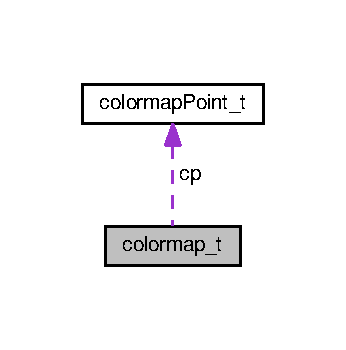
\includegraphics[width=166pt]{structcolormap__t__coll__graph}
\end{center}
\end{figure}
\subsection*{Data Fields}
\begin{DoxyCompactItemize}
\item 
char \hyperlink{structcolormap__t_acd328517a6cf718155c2e6e22b671ca9}{name} \mbox{[}16\mbox{]}
\item 
int \hyperlink{structcolormap__t_a8f4ec518913edf916c0dc3cbb49991b7}{ncp}
\item 
\hyperlink{io_8h_a2bf5ae344b8526b236f7152ce0424670}{colormap\-Point} $\ast$ \hyperlink{structcolormap__t_a64cbb09ad4367b201326341a4b500844}{cp}
\end{DoxyCompactItemize}


\subsection{Detailed Description}


Definition at line 96 of file io.\-h.



\subsection{Field Documentation}
\hypertarget{structcolormap__t_a64cbb09ad4367b201326341a4b500844}{\index{colormap\-\_\-t@{colormap\-\_\-t}!cp@{cp}}
\index{cp@{cp}!colormap_t@{colormap\-\_\-t}}
\subsubsection[{cp}]{\setlength{\rightskip}{0pt plus 5cm}{\bf colormap\-Point}$\ast$ cp}}\label{structcolormap__t_a64cbb09ad4367b201326341a4b500844}


Definition at line 99 of file io.\-h.

\hypertarget{structcolormap__t_acd328517a6cf718155c2e6e22b671ca9}{\index{colormap\-\_\-t@{colormap\-\_\-t}!name@{name}}
\index{name@{name}!colormap_t@{colormap\-\_\-t}}
\subsubsection[{name}]{\setlength{\rightskip}{0pt plus 5cm}char name\mbox{[}16\mbox{]}}}\label{structcolormap__t_acd328517a6cf718155c2e6e22b671ca9}


Definition at line 97 of file io.\-h.

\hypertarget{structcolormap__t_a8f4ec518913edf916c0dc3cbb49991b7}{\index{colormap\-\_\-t@{colormap\-\_\-t}!ncp@{ncp}}
\index{ncp@{ncp}!colormap_t@{colormap\-\_\-t}}
\subsubsection[{ncp}]{\setlength{\rightskip}{0pt plus 5cm}int ncp}}\label{structcolormap__t_a8f4ec518913edf916c0dc3cbb49991b7}


Definition at line 98 of file io.\-h.



The documentation for this struct was generated from the following file\-:\begin{DoxyCompactItemize}
\item 
\hyperlink{io_8h}{io.\-h}\end{DoxyCompactItemize}

\hypertarget{structcolormapPoint__t}{\section{colormap\-Point\-\_\-t Struct Reference}
\label{structcolormapPoint__t}\index{colormap\-Point\-\_\-t@{colormap\-Point\-\_\-t}}
}


{\ttfamily \#include $<$io.\-h$>$}

\subsection*{Data Fields}
\begin{DoxyCompactItemize}
\item 
float \hyperlink{structcolormapPoint__t_a76777b356ab2a080225682528119c4fe}{position}
\item 
float \hyperlink{structcolormapPoint__t_a4788d82c901b9367dd5c0daff8a7616b}{r}
\item 
float \hyperlink{structcolormapPoint__t_a8cf17d727651616de6f2b79ef32170cd}{g}
\item 
float \hyperlink{structcolormapPoint__t_a83fc1af92e29717b4513d121b0c72c7d}{b}
\end{DoxyCompactItemize}


\subsection{Detailed Description}


Definition at line 89 of file io.\-h.



\subsection{Field Documentation}
\hypertarget{structcolormapPoint__t_a83fc1af92e29717b4513d121b0c72c7d}{\index{colormap\-Point\-\_\-t@{colormap\-Point\-\_\-t}!b@{b}}
\index{b@{b}!colormapPoint_t@{colormap\-Point\-\_\-t}}
\subsubsection[{b}]{\setlength{\rightskip}{0pt plus 5cm}float b}}\label{structcolormapPoint__t_a83fc1af92e29717b4513d121b0c72c7d}


Definition at line 93 of file io.\-h.

\hypertarget{structcolormapPoint__t_a8cf17d727651616de6f2b79ef32170cd}{\index{colormap\-Point\-\_\-t@{colormap\-Point\-\_\-t}!g@{g}}
\index{g@{g}!colormapPoint_t@{colormap\-Point\-\_\-t}}
\subsubsection[{g}]{\setlength{\rightskip}{0pt plus 5cm}float g}}\label{structcolormapPoint__t_a8cf17d727651616de6f2b79ef32170cd}


Definition at line 92 of file io.\-h.

\hypertarget{structcolormapPoint__t_a76777b356ab2a080225682528119c4fe}{\index{colormap\-Point\-\_\-t@{colormap\-Point\-\_\-t}!position@{position}}
\index{position@{position}!colormapPoint_t@{colormap\-Point\-\_\-t}}
\subsubsection[{position}]{\setlength{\rightskip}{0pt plus 5cm}float position}}\label{structcolormapPoint__t_a76777b356ab2a080225682528119c4fe}


Definition at line 90 of file io.\-h.

\hypertarget{structcolormapPoint__t_a4788d82c901b9367dd5c0daff8a7616b}{\index{colormap\-Point\-\_\-t@{colormap\-Point\-\_\-t}!r@{r}}
\index{r@{r}!colormapPoint_t@{colormap\-Point\-\_\-t}}
\subsubsection[{r}]{\setlength{\rightskip}{0pt plus 5cm}float r}}\label{structcolormapPoint__t_a4788d82c901b9367dd5c0daff8a7616b}


Definition at line 91 of file io.\-h.



The documentation for this struct was generated from the following file\-:\begin{DoxyCompactItemize}
\item 
\hyperlink{io_8h}{io.\-h}\end{DoxyCompactItemize}

\hypertarget{structdensPotData}{\section{dens\-Pot\-Data Struct Reference}
\label{structdensPotData}\index{dens\-Pot\-Data@{dens\-Pot\-Data}}
}


{\ttfamily \#include $<$global.\-h$>$}

\subsection*{Data Fields}
\begin{DoxyCompactItemize}
\item 
double \hyperlink{structdensPotData_a3b90d5a73541ab9402511d87bed076ef}{v}
\item 
double \hyperlink{structdensPotData_a6f8c052f8417728038991f7f2826d38d}{density}
\end{DoxyCompactItemize}


\subsection{Detailed Description}


Definition at line 151 of file global.\-h.



\subsection{Field Documentation}
\hypertarget{structdensPotData_a6f8c052f8417728038991f7f2826d38d}{\index{dens\-Pot\-Data@{dens\-Pot\-Data}!density@{density}}
\index{density@{density}!densPotData@{dens\-Pot\-Data}}
\subsubsection[{density}]{\setlength{\rightskip}{0pt plus 5cm}double density}}\label{structdensPotData_a6f8c052f8417728038991f7f2826d38d}


Definition at line 153 of file global.\-h.

\hypertarget{structdensPotData_a3b90d5a73541ab9402511d87bed076ef}{\index{dens\-Pot\-Data@{dens\-Pot\-Data}!v@{v}}
\index{v@{v}!densPotData@{dens\-Pot\-Data}}
\subsubsection[{v}]{\setlength{\rightskip}{0pt plus 5cm}double v}}\label{structdensPotData_a3b90d5a73541ab9402511d87bed076ef}


Definition at line 152 of file global.\-h.



The documentation for this struct was generated from the following file\-:\begin{DoxyCompactItemize}
\item 
\hyperlink{global_8h}{global.\-h}\end{DoxyCompactItemize}

\hypertarget{structdoubleVector3d}{\section{double\-Vector3d Struct Reference}
\label{structdoubleVector3d}\index{double\-Vector3d@{double\-Vector3d}}
}


{\ttfamily \#include $<$global.\-h$>$}

\subsection*{Data Fields}
\begin{DoxyCompactItemize}
\item 
double \hyperlink{structdoubleVector3d_af88b946fb90d5f08b5fb740c70e98c10}{x}
\item 
double \hyperlink{structdoubleVector3d_ab927965981178aa1fba979a37168db2a}{y}
\item 
double \hyperlink{structdoubleVector3d_ab3e6ed577a7c669c19de1f9c1b46c872}{z}
\end{DoxyCompactItemize}


\subsection{Detailed Description}


Definition at line 247 of file global.\-h.



\subsection{Field Documentation}
\hypertarget{structdoubleVector3d_af88b946fb90d5f08b5fb740c70e98c10}{\index{double\-Vector3d@{double\-Vector3d}!x@{x}}
\index{x@{x}!doubleVector3d@{double\-Vector3d}}
\subsubsection[{x}]{\setlength{\rightskip}{0pt plus 5cm}double x}}\label{structdoubleVector3d_af88b946fb90d5f08b5fb740c70e98c10}


Definition at line 248 of file global.\-h.

\hypertarget{structdoubleVector3d_ab927965981178aa1fba979a37168db2a}{\index{double\-Vector3d@{double\-Vector3d}!y@{y}}
\index{y@{y}!doubleVector3d@{double\-Vector3d}}
\subsubsection[{y}]{\setlength{\rightskip}{0pt plus 5cm}double y}}\label{structdoubleVector3d_ab927965981178aa1fba979a37168db2a}


Definition at line 249 of file global.\-h.

\hypertarget{structdoubleVector3d_ab3e6ed577a7c669c19de1f9c1b46c872}{\index{double\-Vector3d@{double\-Vector3d}!z@{z}}
\index{z@{z}!doubleVector3d@{double\-Vector3d}}
\subsubsection[{z}]{\setlength{\rightskip}{0pt plus 5cm}double z}}\label{structdoubleVector3d_ab3e6ed577a7c669c19de1f9c1b46c872}


Definition at line 250 of file global.\-h.



The documentation for this struct was generated from the following file\-:\begin{DoxyCompactItemize}
\item 
\hyperlink{global_8h}{global.\-h}\end{DoxyCompactItemize}

\hypertarget{structexpData}{\section{exp\-Data Struct Reference}
\label{structexpData}\index{exp\-Data@{exp\-Data}}
}
\subsection*{Data Fields}
\begin{DoxyCompactItemize}
\item 
int \hyperlink{structexpData_af00601a22186810a9e6d16efb75862ce}{cell}
\item 
int \hyperlink{structexpData_a7e9d757c9982bd721d598bad366fbe62}{proc}
\end{DoxyCompactItemize}


\subsection{Detailed Description}


Definition at line 32 of file comm.\-c.



\subsection{Field Documentation}
\hypertarget{structexpData_af00601a22186810a9e6d16efb75862ce}{\index{exp\-Data@{exp\-Data}!cell@{cell}}
\index{cell@{cell}!expData@{exp\-Data}}
\subsubsection[{cell}]{\setlength{\rightskip}{0pt plus 5cm}int cell}}\label{structexpData_af00601a22186810a9e6d16efb75862ce}


Definition at line 33 of file comm.\-c.

\hypertarget{structexpData_a7e9d757c9982bd721d598bad366fbe62}{\index{exp\-Data@{exp\-Data}!proc@{proc}}
\index{proc@{proc}!expData@{exp\-Data}}
\subsubsection[{proc}]{\setlength{\rightskip}{0pt plus 5cm}int proc}}\label{structexpData_a7e9d757c9982bd721d598bad366fbe62}


Definition at line 34 of file comm.\-c.



The documentation for this struct was generated from the following file\-:\begin{DoxyCompactItemize}
\item 
\hyperlink{comm_8c}{comm.\-c}\end{DoxyCompactItemize}

\hypertarget{structfloatVector3d}{\section{float\-Vector3d Struct Reference}
\label{structfloatVector3d}\index{float\-Vector3d@{float\-Vector3d}}
}


{\ttfamily \#include $<$global.\-h$>$}

\subsection*{Data Fields}
\begin{DoxyCompactItemize}
\item 
float \hyperlink{structfloatVector3d_ad0da36b2558901e21e7a30f6c227a45e}{x}
\item 
float \hyperlink{structfloatVector3d_aa4f0d3eebc3c443f9be81bf48561a217}{y}
\item 
float \hyperlink{structfloatVector3d_af73583b1e980b0aa03f9884812e9fd4d}{z}
\end{DoxyCompactItemize}


\subsection{Detailed Description}


Definition at line 259 of file global.\-h.



\subsection{Field Documentation}
\hypertarget{structfloatVector3d_ad0da36b2558901e21e7a30f6c227a45e}{\index{float\-Vector3d@{float\-Vector3d}!x@{x}}
\index{x@{x}!floatVector3d@{float\-Vector3d}}
\subsubsection[{x}]{\setlength{\rightskip}{0pt plus 5cm}float x}}\label{structfloatVector3d_ad0da36b2558901e21e7a30f6c227a45e}


Definition at line 260 of file global.\-h.

\hypertarget{structfloatVector3d_aa4f0d3eebc3c443f9be81bf48561a217}{\index{float\-Vector3d@{float\-Vector3d}!y@{y}}
\index{y@{y}!floatVector3d@{float\-Vector3d}}
\subsubsection[{y}]{\setlength{\rightskip}{0pt plus 5cm}float y}}\label{structfloatVector3d_aa4f0d3eebc3c443f9be81bf48561a217}


Definition at line 261 of file global.\-h.

\hypertarget{structfloatVector3d_af73583b1e980b0aa03f9884812e9fd4d}{\index{float\-Vector3d@{float\-Vector3d}!z@{z}}
\index{z@{z}!floatVector3d@{float\-Vector3d}}
\subsubsection[{z}]{\setlength{\rightskip}{0pt plus 5cm}float z}}\label{structfloatVector3d_af73583b1e980b0aa03f9884812e9fd4d}


Definition at line 262 of file global.\-h.



The documentation for this struct was generated from the following file\-:\begin{DoxyCompactItemize}
\item 
\hyperlink{global_8h}{global.\-h}\end{DoxyCompactItemize}

\hypertarget{structint64Vector3d}{\section{int64\-Vector3d Struct Reference}
\label{structint64Vector3d}\index{int64\-Vector3d@{int64\-Vector3d}}
}


{\ttfamily \#include $<$global.\-h$>$}

\subsection*{Data Fields}
\begin{DoxyCompactItemize}
\item 
int64\-\_\-t \hyperlink{structint64Vector3d_a040359f45343ce6667f5c66fda5f50e3}{x}
\item 
int64\-\_\-t \hyperlink{structint64Vector3d_a0cbcba26311a97b8e0763317e105a918}{y}
\item 
int64\-\_\-t \hyperlink{structint64Vector3d_a44624880ae3bb63041297b70cb33408b}{z}
\end{DoxyCompactItemize}


\subsection{Detailed Description}


Definition at line 253 of file global.\-h.



\subsection{Field Documentation}
\hypertarget{structint64Vector3d_a040359f45343ce6667f5c66fda5f50e3}{\index{int64\-Vector3d@{int64\-Vector3d}!x@{x}}
\index{x@{x}!int64Vector3d@{int64\-Vector3d}}
\subsubsection[{x}]{\setlength{\rightskip}{0pt plus 5cm}int64\-\_\-t x}}\label{structint64Vector3d_a040359f45343ce6667f5c66fda5f50e3}


Definition at line 254 of file global.\-h.

\hypertarget{structint64Vector3d_a0cbcba26311a97b8e0763317e105a918}{\index{int64\-Vector3d@{int64\-Vector3d}!y@{y}}
\index{y@{y}!int64Vector3d@{int64\-Vector3d}}
\subsubsection[{y}]{\setlength{\rightskip}{0pt plus 5cm}int64\-\_\-t y}}\label{structint64Vector3d_a0cbcba26311a97b8e0763317e105a918}


Definition at line 255 of file global.\-h.

\hypertarget{structint64Vector3d_a44624880ae3bb63041297b70cb33408b}{\index{int64\-Vector3d@{int64\-Vector3d}!z@{z}}
\index{z@{z}!int64Vector3d@{int64\-Vector3d}}
\subsubsection[{z}]{\setlength{\rightskip}{0pt plus 5cm}int64\-\_\-t z}}\label{structint64Vector3d_a44624880ae3bb63041297b70cb33408b}


Definition at line 256 of file global.\-h.



The documentation for this struct was generated from the following file\-:\begin{DoxyCompactItemize}
\item 
\hyperlink{global_8h}{global.\-h}\end{DoxyCompactItemize}

\hypertarget{structpartData}{\section{part\-Data Struct Reference}
\label{structpartData}\index{part\-Data@{part\-Data}}
}


{\ttfamily \#include $<$global.\-h$>$}

\subsection*{Data Fields}
\begin{DoxyCompactItemize}
\item 
double \hyperlink{structpartData_af88b946fb90d5f08b5fb740c70e98c10}{x}
\item 
double \hyperlink{structpartData_ab927965981178aa1fba979a37168db2a}{y}
\item 
double \hyperlink{structpartData_ab3e6ed577a7c669c19de1f9c1b46c872}{z}
\item 
double \hyperlink{structpartData_a8ee9be1b5aa75abae556de3088cba6d9}{h}
\item 
double \hyperlink{structpartData_aba3c5d750d5dbd6e86c11ecaca62885e}{size}
\item 
double \hyperlink{structpartData_a47ec3689b1fd89ba8e75d9a9975ba63f}{young}
\item 
int \hyperlink{structpartData_a13fbf3c17594503f639a7ef768ea73bb}{ctype}
\end{DoxyCompactItemize}


\subsection{Detailed Description}


Definition at line 140 of file global.\-h.



\subsection{Field Documentation}
\hypertarget{structpartData_a13fbf3c17594503f639a7ef768ea73bb}{\index{part\-Data@{part\-Data}!ctype@{ctype}}
\index{ctype@{ctype}!partData@{part\-Data}}
\subsubsection[{ctype}]{\setlength{\rightskip}{0pt plus 5cm}int ctype}}\label{structpartData_a13fbf3c17594503f639a7ef768ea73bb}


Definition at line 147 of file global.\-h.

\hypertarget{structpartData_a8ee9be1b5aa75abae556de3088cba6d9}{\index{part\-Data@{part\-Data}!h@{h}}
\index{h@{h}!partData@{part\-Data}}
\subsubsection[{h}]{\setlength{\rightskip}{0pt plus 5cm}double h}}\label{structpartData_a8ee9be1b5aa75abae556de3088cba6d9}


Definition at line 144 of file global.\-h.

\hypertarget{structpartData_aba3c5d750d5dbd6e86c11ecaca62885e}{\index{part\-Data@{part\-Data}!size@{size}}
\index{size@{size}!partData@{part\-Data}}
\subsubsection[{size}]{\setlength{\rightskip}{0pt plus 5cm}double size}}\label{structpartData_aba3c5d750d5dbd6e86c11ecaca62885e}


Definition at line 145 of file global.\-h.

\hypertarget{structpartData_af88b946fb90d5f08b5fb740c70e98c10}{\index{part\-Data@{part\-Data}!x@{x}}
\index{x@{x}!partData@{part\-Data}}
\subsubsection[{x}]{\setlength{\rightskip}{0pt plus 5cm}double x}}\label{structpartData_af88b946fb90d5f08b5fb740c70e98c10}


Definition at line 141 of file global.\-h.

\hypertarget{structpartData_ab927965981178aa1fba979a37168db2a}{\index{part\-Data@{part\-Data}!y@{y}}
\index{y@{y}!partData@{part\-Data}}
\subsubsection[{y}]{\setlength{\rightskip}{0pt plus 5cm}double y}}\label{structpartData_ab927965981178aa1fba979a37168db2a}


Definition at line 142 of file global.\-h.

\hypertarget{structpartData_a47ec3689b1fd89ba8e75d9a9975ba63f}{\index{part\-Data@{part\-Data}!young@{young}}
\index{young@{young}!partData@{part\-Data}}
\subsubsection[{young}]{\setlength{\rightskip}{0pt plus 5cm}double young}}\label{structpartData_a47ec3689b1fd89ba8e75d9a9975ba63f}


Definition at line 146 of file global.\-h.

\hypertarget{structpartData_ab3e6ed577a7c669c19de1f9c1b46c872}{\index{part\-Data@{part\-Data}!z@{z}}
\index{z@{z}!partData@{part\-Data}}
\subsubsection[{z}]{\setlength{\rightskip}{0pt plus 5cm}double z}}\label{structpartData_ab3e6ed577a7c669c19de1f9c1b46c872}


Definition at line 143 of file global.\-h.



The documentation for this struct was generated from the following file\-:\begin{DoxyCompactItemize}
\item 
\hyperlink{global_8h}{global.\-h}\end{DoxyCompactItemize}

\hypertarget{structstatisticsData}{\section{statistics\-Data Struct Reference}
\label{structstatisticsData}\index{statistics\-Data@{statistics\-Data}}
}


{\ttfamily \#include $<$global.\-h$>$}

\subsection*{Data Fields}
\begin{DoxyCompactItemize}
\item 
double \hyperlink{structstatisticsData_ad99dc4104d1898b6e593bbf331e41c69}{minsize}
\item 
double \hyperlink{structstatisticsData_a7383c898fd4cd4d862ca65d3713086cd}{maxsize}
\item 
double \hyperlink{structstatisticsData_a78455d23ec97258967b76cbb2332b7be}{mindist}
\item 
double \hyperlink{structstatisticsData_a485292d20f5d14bd18e83fef65976fb4}{maxvel}
\item 
double \hyperlink{structstatisticsData_a1b9d00ac67b4ceca8e7747a50edc802b}{minvel}
\item 
double \hyperlink{structstatisticsData_abc8b83844f3405d9046189aa841b48fd}{maxdens}
\item 
double \hyperlink{structstatisticsData_a2ddb05b9ae611dab07eef62db427ed61}{mindens}
\item 
double \hyperlink{structstatisticsData_a62a3935a35dda8e375bf0ec6cc160d5e}{densdev}
\item 
double \hyperlink{structstatisticsData_ae897d6b29710ca63a31e17866c73bc9a}{densavg}
\end{DoxyCompactItemize}


\subsection{Detailed Description}


Definition at line 289 of file global.\-h.



\subsection{Field Documentation}
\hypertarget{structstatisticsData_ae897d6b29710ca63a31e17866c73bc9a}{\index{statistics\-Data@{statistics\-Data}!densavg@{densavg}}
\index{densavg@{densavg}!statisticsData@{statistics\-Data}}
\subsubsection[{densavg}]{\setlength{\rightskip}{0pt plus 5cm}double densavg}}\label{structstatisticsData_ae897d6b29710ca63a31e17866c73bc9a}


Definition at line 298 of file global.\-h.

\hypertarget{structstatisticsData_a62a3935a35dda8e375bf0ec6cc160d5e}{\index{statistics\-Data@{statistics\-Data}!densdev@{densdev}}
\index{densdev@{densdev}!statisticsData@{statistics\-Data}}
\subsubsection[{densdev}]{\setlength{\rightskip}{0pt plus 5cm}double densdev}}\label{structstatisticsData_a62a3935a35dda8e375bf0ec6cc160d5e}


Definition at line 297 of file global.\-h.

\hypertarget{structstatisticsData_abc8b83844f3405d9046189aa841b48fd}{\index{statistics\-Data@{statistics\-Data}!maxdens@{maxdens}}
\index{maxdens@{maxdens}!statisticsData@{statistics\-Data}}
\subsubsection[{maxdens}]{\setlength{\rightskip}{0pt plus 5cm}double maxdens}}\label{structstatisticsData_abc8b83844f3405d9046189aa841b48fd}


Definition at line 295 of file global.\-h.

\hypertarget{structstatisticsData_a7383c898fd4cd4d862ca65d3713086cd}{\index{statistics\-Data@{statistics\-Data}!maxsize@{maxsize}}
\index{maxsize@{maxsize}!statisticsData@{statistics\-Data}}
\subsubsection[{maxsize}]{\setlength{\rightskip}{0pt plus 5cm}double maxsize}}\label{structstatisticsData_a7383c898fd4cd4d862ca65d3713086cd}


Definition at line 291 of file global.\-h.

\hypertarget{structstatisticsData_a485292d20f5d14bd18e83fef65976fb4}{\index{statistics\-Data@{statistics\-Data}!maxvel@{maxvel}}
\index{maxvel@{maxvel}!statisticsData@{statistics\-Data}}
\subsubsection[{maxvel}]{\setlength{\rightskip}{0pt plus 5cm}double maxvel}}\label{structstatisticsData_a485292d20f5d14bd18e83fef65976fb4}


Definition at line 293 of file global.\-h.

\hypertarget{structstatisticsData_a2ddb05b9ae611dab07eef62db427ed61}{\index{statistics\-Data@{statistics\-Data}!mindens@{mindens}}
\index{mindens@{mindens}!statisticsData@{statistics\-Data}}
\subsubsection[{mindens}]{\setlength{\rightskip}{0pt plus 5cm}double mindens}}\label{structstatisticsData_a2ddb05b9ae611dab07eef62db427ed61}


Definition at line 296 of file global.\-h.

\hypertarget{structstatisticsData_a78455d23ec97258967b76cbb2332b7be}{\index{statistics\-Data@{statistics\-Data}!mindist@{mindist}}
\index{mindist@{mindist}!statisticsData@{statistics\-Data}}
\subsubsection[{mindist}]{\setlength{\rightskip}{0pt plus 5cm}double mindist}}\label{structstatisticsData_a78455d23ec97258967b76cbb2332b7be}


Definition at line 292 of file global.\-h.

\hypertarget{structstatisticsData_ad99dc4104d1898b6e593bbf331e41c69}{\index{statistics\-Data@{statistics\-Data}!minsize@{minsize}}
\index{minsize@{minsize}!statisticsData@{statistics\-Data}}
\subsubsection[{minsize}]{\setlength{\rightskip}{0pt plus 5cm}double minsize}}\label{structstatisticsData_ad99dc4104d1898b6e593bbf331e41c69}


Definition at line 290 of file global.\-h.

\hypertarget{structstatisticsData_a1b9d00ac67b4ceca8e7747a50edc802b}{\index{statistics\-Data@{statistics\-Data}!minvel@{minvel}}
\index{minvel@{minvel}!statisticsData@{statistics\-Data}}
\subsubsection[{minvel}]{\setlength{\rightskip}{0pt plus 5cm}double minvel}}\label{structstatisticsData_a1b9d00ac67b4ceca8e7747a50edc802b}


Definition at line 294 of file global.\-h.



The documentation for this struct was generated from the following file\-:\begin{DoxyCompactItemize}
\item 
\hyperlink{global_8h}{global.\-h}\end{DoxyCompactItemize}

\hypertarget{structuintVector3d}{\section{uint\-Vector3d Struct Reference}
\label{structuintVector3d}\index{uint\-Vector3d@{uint\-Vector3d}}
}


{\ttfamily \#include $<$global.\-h$>$}

\subsection*{Data Fields}
\begin{DoxyCompactItemize}
\item 
unsigned int \hyperlink{structuintVector3d_a676e0da0ef83bbbdf42538e54b97506b}{x}
\item 
unsigned int \hyperlink{structuintVector3d_ac30de26db5f6d1c18c63913729adca7d}{y}
\item 
unsigned int \hyperlink{structuintVector3d_a3d99b005d0fb73033dce14d4a135d01f}{z}
\end{DoxyCompactItemize}


\subsection{Detailed Description}


Definition at line 265 of file global.\-h.



\subsection{Field Documentation}
\hypertarget{structuintVector3d_a676e0da0ef83bbbdf42538e54b97506b}{\index{uint\-Vector3d@{uint\-Vector3d}!x@{x}}
\index{x@{x}!uintVector3d@{uint\-Vector3d}}
\subsubsection[{x}]{\setlength{\rightskip}{0pt plus 5cm}unsigned int x}}\label{structuintVector3d_a676e0da0ef83bbbdf42538e54b97506b}


Definition at line 266 of file global.\-h.

\hypertarget{structuintVector3d_ac30de26db5f6d1c18c63913729adca7d}{\index{uint\-Vector3d@{uint\-Vector3d}!y@{y}}
\index{y@{y}!uintVector3d@{uint\-Vector3d}}
\subsubsection[{y}]{\setlength{\rightskip}{0pt plus 5cm}unsigned int y}}\label{structuintVector3d_ac30de26db5f6d1c18c63913729adca7d}


Definition at line 267 of file global.\-h.

\hypertarget{structuintVector3d_a3d99b005d0fb73033dce14d4a135d01f}{\index{uint\-Vector3d@{uint\-Vector3d}!z@{z}}
\index{z@{z}!uintVector3d@{uint\-Vector3d}}
\subsubsection[{z}]{\setlength{\rightskip}{0pt plus 5cm}unsigned int z}}\label{structuintVector3d_a3d99b005d0fb73033dce14d4a135d01f}


Definition at line 268 of file global.\-h.



The documentation for this struct was generated from the following file\-:\begin{DoxyCompactItemize}
\item 
\hyperlink{global_8h}{global.\-h}\end{DoxyCompactItemize}

\chapter{File Documentation}
\hypertarget{bone_8c}{\section{bone.\-c File Reference}
\label{bone_8c}\index{bone.\-c@{bone.\-c}}
}


contains functions defining virtual bone structure  


{\ttfamily \#include $<$stdio.\-h$>$}\\*
{\ttfamily \#include $<$stdlib.\-h$>$}\\*
{\ttfamily \#include $<$mpi.\-h$>$}\\*
{\ttfamily \#include $<$math.\-h$>$}\\*
{\ttfamily \#include $<$inttypes.\-h$>$}\\*
{\ttfamily \#include $<$sprng.\-h$>$}\\*
{\ttfamily \#include $<$float.\-h$>$}\\*
{\ttfamily \#include \char`\"{}global.\-h\char`\"{}}\\*
Include dependency graph for bone.\-c\-:\nopagebreak
\begin{figure}[H]
\begin{center}
\leavevmode
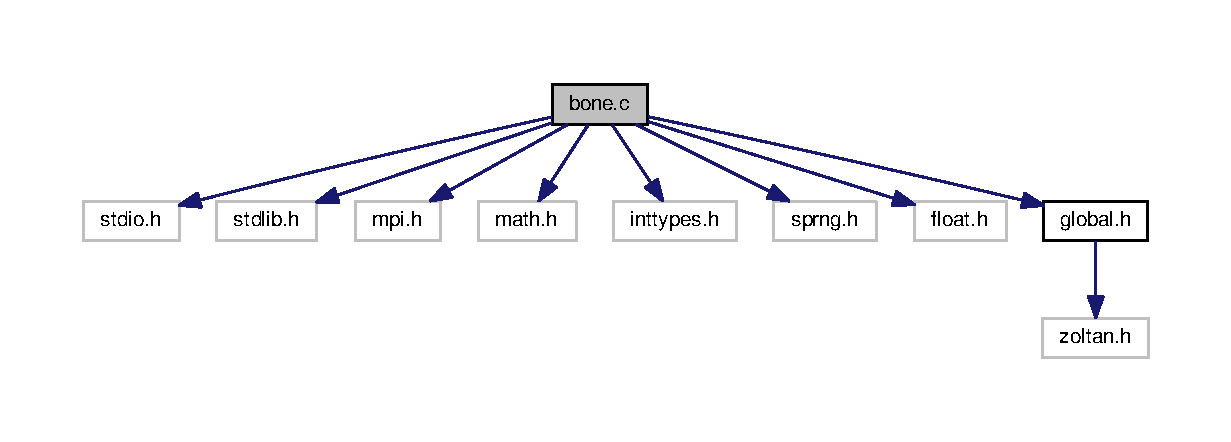
\includegraphics[width=350pt]{bone_8c__incl}
\end{center}
\end{figure}
\subsection*{Functions}
\begin{DoxyCompactItemize}
\item 
int \hyperlink{bone_8c_a76de0ed6535f866cc17a6eb1b7cf1350}{init\-Bone} ()
\end{DoxyCompactItemize}


\subsection{Detailed Description}
contains functions defining virtual bone structure 

Definition in file \hyperlink{bone_8c_source}{bone.\-c}.



\subsection{Function Documentation}
\hypertarget{bone_8c_a76de0ed6535f866cc17a6eb1b7cf1350}{\index{bone.\-c@{bone.\-c}!init\-Bone@{init\-Bone}}
\index{init\-Bone@{init\-Bone}!bone.c@{bone.\-c}}
\subsubsection[{init\-Bone}]{\setlength{\rightskip}{0pt plus 5cm}int init\-Bone (
\begin{DoxyParamCaption}
{}
\end{DoxyParamCaption}
)}}\label{bone_8c_a76de0ed6535f866cc17a6eb1b7cf1350}
This functions builds a bone structure from available data. 

Definition at line 40 of file bone.\-c.



References cell\-Data\-::age, bnc, cells, csize, cell\-Data\-::ctype, cell\-Data\-::death, cell\-Data\-::density, cell\-Data\-::g1, g1, cell\-Data\-::g2, g2, cell\-Data\-::gid, cell\-Data\-::h, cell\-Data\-::halo, lbnc, lnc, local\-Cell\-Count, local\-I\-D, cell\-Data\-::m, m, max\-Cells\-Per\-Proc, M\-P\-Irank, number\-Of\-Counts, cell\-Data\-::phase, cell\-Data\-::phasetime, cell\-Data\-::s, s, cell\-Data\-::size, stream, total\-Cell\-Count, cell\-Data\-::tumor, cell\-Data\-::v, v, cell\-Data\-::x, cell\-Data\-::y, cell\-Data\-::young, and cell\-Data\-::z.


\begin{DoxyCode}
41 \{
42   \textcolor{keywordtype}{int} i,j,k;
43   \textcolor{keywordtype}{int} \hyperlink{global_8h_ac51334f57ef8b81c0629c9421798c344}{m};
44   \textcolor{keywordtype}{int} ax,ay,az;
45   \textcolor{keywordtype}{double} ox,oy,oz;
46   \textcolor{keywordtype}{double} v0x,v0y,v0z;
47   \textcolor{keywordtype}{double} v1x,v1y,v1z;
48   \textcolor{keywordtype}{double} v2x,v2y,v2z;
49   \textcolor{keywordtype}{char} text[256];
50   \textcolor{keywordtype}{int} ***data;
51   \textcolor{keywordtype}{int} d1,d2;
52   \textcolor{keywordtype}{int} ret;
53 
54   \textcolor{keywordtype}{double} minx,miny,minz;
55   \textcolor{keywordtype}{double} maxx,maxy,maxz;
56 
57   \hyperlink{global_8h_ad1705f0ec3f18de6cc969492145b531b}{bnc}=0;
58   \hyperlink{global_8h_a0cb9f3a12f8c024f27273125d2f07efb}{lbnc}=0;
59 
60   \textcolor{keywordflow}{if}(\hyperlink{global_8h_a710288ab7d2734acc4566a87a645325d}{MPIrank}==0) \{
61     FILE *fh1,*fh2;
62     \textcolor{keywordflow}{if}(!(fh1=fopen(\textcolor{stringliteral}{"bones.txt"},\textcolor{stringliteral}{"r"}))) \{
63       printf(\textcolor{stringliteral}{"File bones.txt not found\(\backslash\)n"});
64       exit(1);
65     \}
66     \textcolor{keywordflow}{if}(!(fh2=fopen(\textcolor{stringliteral}{"bones.vnf"},\textcolor{stringliteral}{"r"}))) \{
67       printf(\textcolor{stringliteral}{"File bones.vnf not found\(\backslash\)n"});
68       exit(1);
69     \}
70     minx=DBL\_MAX;
71     miny=DBL\_MAX;
72     minz=DBL\_MAX;
73     maxx=-DBL\_MAX;
74     maxy=-DBL\_MAX;
75     maxz=-DBL\_MAX;
76 
77     \textcolor{comment}{/* start with the .vnf file */}
78     \textcolor{comment}{/* skip the header */}
79     ret=fscanf(fh2,\textcolor{stringliteral}{"%*[^\(\backslash\)n]\(\backslash\)n"});
80     \textcolor{comment}{/* read dimensions */}
81     ret=fscanf(fh2,\textcolor{stringliteral}{"%s"},text);
82     \textcolor{keywordflow}{if}(strcmp(text,\textcolor{stringliteral}{"dims"})==0) \{
83       ret=fscanf(fh2,\textcolor{stringliteral}{"%d %d %d\(\backslash\)n"},&ax,&ay,&az);
84     \}
85     \textcolor{comment}{/* read 3d box */}
86     ret=fscanf(fh2,\textcolor{stringliteral}{"%s"},text);
87     \textcolor{keywordflow}{if}(strcmp(text,\textcolor{stringliteral}{"origin"})==0) \{
88       ret=fscanf(fh2,\textcolor{stringliteral}{"%lf %lf %lf\(\backslash\)n"},&ox,&oy,&oz);
89     \}
90     ret=fscanf(fh2,\textcolor{stringliteral}{"%s"},text);
91     \textcolor{keywordflow}{if}(strcmp(text,\textcolor{stringliteral}{"v0"})==0) \{
92       ret=fscanf(fh2,\textcolor{stringliteral}{"%lf %lf %lf\(\backslash\)n"},&v0x,&v0y,&v0z);
93     \}
94     ret=fscanf(fh2,\textcolor{stringliteral}{"%s"},text);
95     \textcolor{keywordflow}{if}(strcmp(text,\textcolor{stringliteral}{"v1"})==0) \{
96       ret=fscanf(fh2,\textcolor{stringliteral}{"%lf %lf %lf\(\backslash\)n"},&v1x,&v1y,&v1z);
97     \}
98     ret=fscanf(fh2,\textcolor{stringliteral}{"%s"},text);
99     \textcolor{keywordflow}{if}(strcmp(text,\textcolor{stringliteral}{"v2"})==0) \{
100       ret=fscanf(fh2,\textcolor{stringliteral}{"%lf %lf %lf\(\backslash\)n"},&v2x,&v2y,&v2z);
101     \}
102     \textcolor{comment}{/* print info */}
103     printf(\textcolor{stringliteral}{"Dimensions: %d %d %d\(\backslash\)nOrigin: %lf %lf %lf\(\backslash\)n"},ax,ay,az,ox,oy,oz);
104     printf(\textcolor{stringliteral}{"v0: %lf %lf %lf\(\backslash\)nv1: %lf %lf %lf\(\backslash\)nv2: %lf %lf %lf\(\backslash\)n"},v0x,v0y,v0z,v1x,v1y,v1z,v2x,v2y,v2z);
105     \textcolor{comment}{/* allocate data table */}
106     data=(\textcolor{keywordtype}{int}***)malloc(ax*\textcolor{keyword}{sizeof}(\textcolor{keywordtype}{int}**));
107     \textcolor{keywordflow}{for}(i=0; i<ax; i++) \{
108       data[i]=(\textcolor{keywordtype}{int}**)malloc(ay*\textcolor{keyword}{sizeof}(\textcolor{keywordtype}{int}*));
109       \textcolor{keywordflow}{for}(j=0; j<ay; j++) \{
110         data[i][j]=(\textcolor{keywordtype}{int}*)malloc(az*\textcolor{keyword}{sizeof}(\textcolor{keywordtype}{int}));
111       \}
112     \}
113 
114     \textcolor{comment}{/* now .txt file */}
115     \textcolor{comment}{/* skip the header */}
116     ret=fscanf(fh1,\textcolor{stringliteral}{"%*[^\(\backslash\)n]\(\backslash\)n"});
117     \textcolor{comment}{/* read data */}
118     \textcolor{keywordflow}{for}(k=0; k<az; k++)
119       \textcolor{keywordflow}{for}(j=0; j<ay; j++)
120         \textcolor{keywordflow}{for}(i=0; i<ax; i++) \{
121           ret=fscanf(fh1,\textcolor{stringliteral}{"%d %d\(\backslash\)n"},&d1,&d2);
122           data[i][j][k]=d1;
123         \}
124 
125     \textcolor{comment}{/* compute coordinates - use origin,v0,v1,v2 */}
126     \textcolor{keywordflow}{for}(i=0; i<ax; i++)
127       \textcolor{keywordflow}{for}(j=0; j<ay; j++)
128         \textcolor{keywordflow}{for}(k=0; k<az; k++) \{
129           \textcolor{keywordflow}{if} (data[i][j][k]==2) \{
130             \hyperlink{global_8h_a3ea537bde8d64e54770a2bd81e3f00be}{cells}[\hyperlink{global_8h_a7065c019590815f10169c219f358e7d0}{lnc}].\hyperlink{structcellData_aba3c5d750d5dbd6e86c11ecaca62885e}{size}=pow(2.0, -(1.0 / 3.0)) * \hyperlink{global_8h_a39fd0cf73801b603ea78d20e05d8cfd3}{csize};\textcolor{comment}{//csize;}
131             \hyperlink{global_8h_a3ea537bde8d64e54770a2bd81e3f00be}{cells}[\hyperlink{global_8h_a7065c019590815f10169c219f358e7d0}{lnc}].\hyperlink{structcellData_af88b946fb90d5f08b5fb740c70e98c10}{x}=ox + i*v0x + j*v1x + k*v2x;
132             \hyperlink{global_8h_a3ea537bde8d64e54770a2bd81e3f00be}{cells}[\hyperlink{global_8h_a7065c019590815f10169c219f358e7d0}{lnc}].\hyperlink{structcellData_ab927965981178aa1fba979a37168db2a}{y}=oy + i*v0y + j*v1y + k*v2y;
133             \hyperlink{global_8h_a3ea537bde8d64e54770a2bd81e3f00be}{cells}[\hyperlink{global_8h_a7065c019590815f10169c219f358e7d0}{lnc}].\hyperlink{structcellData_ab3e6ed577a7c669c19de1f9c1b46c872}{z}=oz + i*v0z + j*v1z + k*v2z;
134             maxx=(\hyperlink{global_8h_a3ea537bde8d64e54770a2bd81e3f00be}{cells}[\hyperlink{global_8h_a7065c019590815f10169c219f358e7d0}{lnc}].\hyperlink{structcellData_af88b946fb90d5f08b5fb740c70e98c10}{x}>maxx?\hyperlink{global_8h_a3ea537bde8d64e54770a2bd81e3f00be}{cells}[\hyperlink{global_8h_a7065c019590815f10169c219f358e7d0}{lnc}].\hyperlink{structcellData_af88b946fb90d5f08b5fb740c70e98c10}{x}:maxx);
135             maxy=(\hyperlink{global_8h_a3ea537bde8d64e54770a2bd81e3f00be}{cells}[\hyperlink{global_8h_a7065c019590815f10169c219f358e7d0}{lnc}].\hyperlink{structcellData_ab927965981178aa1fba979a37168db2a}{y}>maxy?\hyperlink{global_8h_a3ea537bde8d64e54770a2bd81e3f00be}{cells}[\hyperlink{global_8h_a7065c019590815f10169c219f358e7d0}{lnc}].\hyperlink{structcellData_ab927965981178aa1fba979a37168db2a}{y}:maxy);
136             maxz=(\hyperlink{global_8h_a3ea537bde8d64e54770a2bd81e3f00be}{cells}[\hyperlink{global_8h_a7065c019590815f10169c219f358e7d0}{lnc}].\hyperlink{structcellData_ab3e6ed577a7c669c19de1f9c1b46c872}{z}>maxz?\hyperlink{global_8h_a3ea537bde8d64e54770a2bd81e3f00be}{cells}[\hyperlink{global_8h_a7065c019590815f10169c219f358e7d0}{lnc}].\hyperlink{structcellData_ab3e6ed577a7c669c19de1f9c1b46c872}{z}:maxz);
137             minx=(\hyperlink{global_8h_a3ea537bde8d64e54770a2bd81e3f00be}{cells}[\hyperlink{global_8h_a7065c019590815f10169c219f358e7d0}{lnc}].\hyperlink{structcellData_af88b946fb90d5f08b5fb740c70e98c10}{x}<minx?\hyperlink{global_8h_a3ea537bde8d64e54770a2bd81e3f00be}{cells}[\hyperlink{global_8h_a7065c019590815f10169c219f358e7d0}{lnc}].\hyperlink{structcellData_af88b946fb90d5f08b5fb740c70e98c10}{x}:minx);
138             miny=(\hyperlink{global_8h_a3ea537bde8d64e54770a2bd81e3f00be}{cells}[\hyperlink{global_8h_a7065c019590815f10169c219f358e7d0}{lnc}].\hyperlink{structcellData_ab927965981178aa1fba979a37168db2a}{y}<miny?\hyperlink{global_8h_a3ea537bde8d64e54770a2bd81e3f00be}{cells}[\hyperlink{global_8h_a7065c019590815f10169c219f358e7d0}{lnc}].\hyperlink{structcellData_ab927965981178aa1fba979a37168db2a}{y}:miny);
139             minz=(\hyperlink{global_8h_a3ea537bde8d64e54770a2bd81e3f00be}{cells}[\hyperlink{global_8h_a7065c019590815f10169c219f358e7d0}{lnc}].\hyperlink{structcellData_ab3e6ed577a7c669c19de1f9c1b46c872}{z}<minz?\hyperlink{global_8h_a3ea537bde8d64e54770a2bd81e3f00be}{cells}[\hyperlink{global_8h_a7065c019590815f10169c219f358e7d0}{lnc}].\hyperlink{structcellData_ab3e6ed577a7c669c19de1f9c1b46c872}{z}:minz);
140 
141             \hyperlink{global_8h_a3ea537bde8d64e54770a2bd81e3f00be}{cells}[\hyperlink{global_8h_a7065c019590815f10169c219f358e7d0}{lnc}].\hyperlink{structcellData_abb4d4bd9231e9f994e87f32cc4fcfce8}{gid} =
142               (\textcolor{keywordtype}{unsigned} \textcolor{keywordtype}{long} \textcolor{keywordtype}{long} int) \hyperlink{global_8h_a710288ab7d2734acc4566a87a645325d}{MPIrank} *(\textcolor{keywordtype}{unsigned} \textcolor{keywordtype}{long} \textcolor{keywordtype}{long} \textcolor{keywordtype}{int})
143               \hyperlink{global_8h_a2de426dd266cfdaaf6fb52ba3dc2740a}{maxCellsPerProc} + (\textcolor{keywordtype}{unsigned} \textcolor{keywordtype}{long} \textcolor{keywordtype}{long} int) \hyperlink{global_8h_a7065c019590815f10169c219f358e7d0}{lnc};
144             \hyperlink{global_8h_a3ea537bde8d64e54770a2bd81e3f00be}{cells}[\hyperlink{global_8h_a7065c019590815f10169c219f358e7d0}{lnc}].\hyperlink{structcellData_a3b90d5a73541ab9402511d87bed076ef}{v} = 0.0;
145             \hyperlink{global_8h_a3ea537bde8d64e54770a2bd81e3f00be}{cells}[\hyperlink{global_8h_a7065c019590815f10169c219f358e7d0}{lnc}].\hyperlink{structcellData_a6f8c052f8417728038991f7f2826d38d}{density} = 0.0;
146             \hyperlink{global_8h_a3ea537bde8d64e54770a2bd81e3f00be}{cells}[\hyperlink{global_8h_a7065c019590815f10169c219f358e7d0}{lnc}].\hyperlink{structcellData_a8ee9be1b5aa75abae556de3088cba6d9}{h} = 3*\hyperlink{global_8h_a39fd0cf73801b603ea78d20e05d8cfd3}{csize};\textcolor{comment}{//h;}
147             \hyperlink{global_8h_a3ea537bde8d64e54770a2bd81e3f00be}{cells}[\hyperlink{global_8h_a7065c019590815f10169c219f358e7d0}{lnc}].\hyperlink{structcellData_ad0bd87a264e65d1c17ecc07049819f2c}{young} = 2100.0 + sprng(\hyperlink{global_8h_a5340130b6fb2647cef6b71354e27b0d4}{stream}) * 100.0;
148             \hyperlink{global_8h_a3ea537bde8d64e54770a2bd81e3f00be}{cells}[\hyperlink{global_8h_a7065c019590815f10169c219f358e7d0}{lnc}].\hyperlink{structcellData_a80ff3fcc4d03d0b1b01559839d12df5b}{halo} = 0;
149             \hyperlink{global_8h_a3ea537bde8d64e54770a2bd81e3f00be}{cells}[\hyperlink{global_8h_a7065c019590815f10169c219f358e7d0}{lnc}].\hyperlink{structcellData_accf3aec63bc20b3c99ab4881cb07c05b}{phase} = 0;
150             \hyperlink{global_8h_a3ea537bde8d64e54770a2bd81e3f00be}{cells}[\hyperlink{global_8h_a7065c019590815f10169c219f358e7d0}{lnc}].\hyperlink{structcellData_a581debe7d16bce9d187b97855f4e99d4}{g1} = \hyperlink{global_8h_a581debe7d16bce9d187b97855f4e99d4}{g1} * (1 + (sprng(\hyperlink{global_8h_a5340130b6fb2647cef6b71354e27b0d4}{stream}) * 2 - 1) * 
      \hyperlink{global_8h_a48d9522e58fa05906c6dba23e5745a72}{v});
151             \hyperlink{global_8h_a3ea537bde8d64e54770a2bd81e3f00be}{cells}[\hyperlink{global_8h_a7065c019590815f10169c219f358e7d0}{lnc}].\hyperlink{structcellData_aee9971139118d56815564304450c4775}{g2} = \hyperlink{global_8h_aee9971139118d56815564304450c4775}{g2} * (1 + (sprng(\hyperlink{global_8h_a5340130b6fb2647cef6b71354e27b0d4}{stream}) * 2 - 1) * 
      \hyperlink{global_8h_a48d9522e58fa05906c6dba23e5745a72}{v});
152             \hyperlink{global_8h_a3ea537bde8d64e54770a2bd81e3f00be}{cells}[\hyperlink{global_8h_a7065c019590815f10169c219f358e7d0}{lnc}].\hyperlink{structcellData_a874f74a4dc1c9a0cd9c6e0d79c298f55}{s} = \hyperlink{global_8h_a874f74a4dc1c9a0cd9c6e0d79c298f55}{s} * (1 + (sprng(\hyperlink{global_8h_a5340130b6fb2647cef6b71354e27b0d4}{stream}) * 2 - 1) * \hyperlink{global_8h_a48d9522e58fa05906c6dba23e5745a72}{v});
153             \hyperlink{global_8h_a3ea537bde8d64e54770a2bd81e3f00be}{cells}[\hyperlink{global_8h_a7065c019590815f10169c219f358e7d0}{lnc}].\hyperlink{structcellData_ac51334f57ef8b81c0629c9421798c344}{m} = m * (1 + (sprng(\hyperlink{global_8h_a5340130b6fb2647cef6b71354e27b0d4}{stream}) * 2 - 1) * \hyperlink{global_8h_a48d9522e58fa05906c6dba23e5745a72}{v});
154             \hyperlink{global_8h_a3ea537bde8d64e54770a2bd81e3f00be}{cells}[\hyperlink{global_8h_a7065c019590815f10169c219f358e7d0}{lnc}].\hyperlink{structcellData_afe1297f954440c453b59fcb06992dbd5}{phasetime} = 0.0;
155             \hyperlink{global_8h_a3ea537bde8d64e54770a2bd81e3f00be}{cells}[\hyperlink{global_8h_a7065c019590815f10169c219f358e7d0}{lnc}].\hyperlink{structcellData_a91d98a856bbd96810b40af3ca5cc901a}{age} = 0;
156             \hyperlink{global_8h_a3ea537bde8d64e54770a2bd81e3f00be}{cells}[\hyperlink{global_8h_a7065c019590815f10169c219f358e7d0}{lnc}].\hyperlink{structcellData_add1e1533be6e693ffedcdbafdf8b855c}{death} = 0;
157             \hyperlink{global_8h_a3ea537bde8d64e54770a2bd81e3f00be}{cells}[\hyperlink{global_8h_a7065c019590815f10169c219f358e7d0}{lnc}].\hyperlink{structcellData_a49af8c5336d6c2401bc24f86dbb97b36}{tumor} = 0;
158             \textcolor{comment}{/* tag bone cell */}
159             \hyperlink{global_8h_a3ea537bde8d64e54770a2bd81e3f00be}{cells}[\hyperlink{global_8h_a7065c019590815f10169c219f358e7d0}{lnc}].\hyperlink{structcellData_a13fbf3c17594503f639a7ef768ea73bb}{ctype} = 3;
160 
161             \hyperlink{global_8h_a7065c019590815f10169c219f358e7d0}{lnc}++;
162             \hyperlink{global_8h_a0cb9f3a12f8c024f27273125d2f07efb}{lbnc}++;
163             \hyperlink{global_8h_a265cb7ee626de517ecec0f0ac60833a7}{localID}++;
164 
165           \}
166         \}
167     fclose(fh1);
168     fclose(fh2);
169   \}
170 
171   \textcolor{keywordflow}{for}(i=0; i<\hyperlink{global_8h_a7065c019590815f10169c219f358e7d0}{lnc}; i++) \{
172     \hyperlink{global_8h_a3ea537bde8d64e54770a2bd81e3f00be}{cells}[i].\hyperlink{structcellData_af88b946fb90d5f08b5fb740c70e98c10}{x}-=minx;
173     \hyperlink{global_8h_a3ea537bde8d64e54770a2bd81e3f00be}{cells}[i].\hyperlink{structcellData_ab927965981178aa1fba979a37168db2a}{y}-=miny;
174     \hyperlink{global_8h_a3ea537bde8d64e54770a2bd81e3f00be}{cells}[i].\hyperlink{structcellData_ab3e6ed577a7c669c19de1f9c1b46c872}{z}-=minz;
175   \}
176 
177   MPI\_Allreduce(\hyperlink{global_8h_ab7a46ee61df03f5b6a569427a2f50bec}{localCellCount}, \hyperlink{global_8h_af1a14df9e6c8efece5183d9625039587}{totalCellCount}, 
      \hyperlink{global_8h_a97c5d6b146e57ace62a66400c433aa4d}{numberOfCounts},
178                 MPI\_INT64\_T, MPI\_SUM, MPI\_COMM\_WORLD);
179 
180   \textcolor{comment}{/* free data */}
181   \textcolor{keywordflow}{for}(i=0; i<ax; i++) \{
182     \textcolor{keywordflow}{for}(j=0; j<ay; j++)
183       free(data[i][j]);
184     free(data[i]);
185   \}
186   free(data);
187 
188   \textcolor{keywordflow}{return} 0;
189 \}
\end{DoxyCode}


Here is the caller graph for this function\-:\nopagebreak
\begin{figure}[H]
\begin{center}
\leavevmode
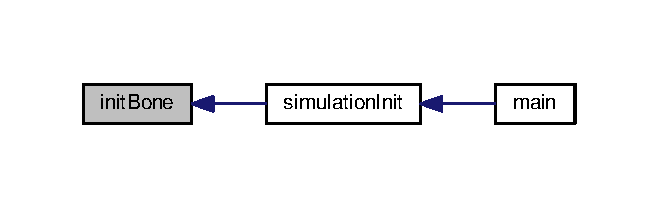
\includegraphics[width=316pt]{bone_8c_a76de0ed6535f866cc17a6eb1b7cf1350_icgraph}
\end{center}
\end{figure}



\hypertarget{cells_8c}{\section{cells.\-c File Reference}
\label{cells_8c}\index{cells.\-c@{cells.\-c}}
}


contains functions which control current states and evolution of cells  


{\ttfamily \#include $<$stdio.\-h$>$}\\*
{\ttfamily \#include $<$stdlib.\-h$>$}\\*
{\ttfamily \#include $<$mpi.\-h$>$}\\*
{\ttfamily \#include $<$math.\-h$>$}\\*
{\ttfamily \#include $<$inttypes.\-h$>$}\\*
{\ttfamily \#include $<$sprng.\-h$>$}\\*
{\ttfamily \#include $<$float.\-h$>$}\\*
{\ttfamily \#include \char`\"{}global.\-h\char`\"{}}\\*
{\ttfamily \#include \char`\"{}inline.\-h\char`\"{}}\\*
{\ttfamily \#include \char`\"{}fields.\-h\char`\"{}}\\*
Include dependency graph for cells.\-c\-:\nopagebreak
\begin{figure}[H]
\begin{center}
\leavevmode
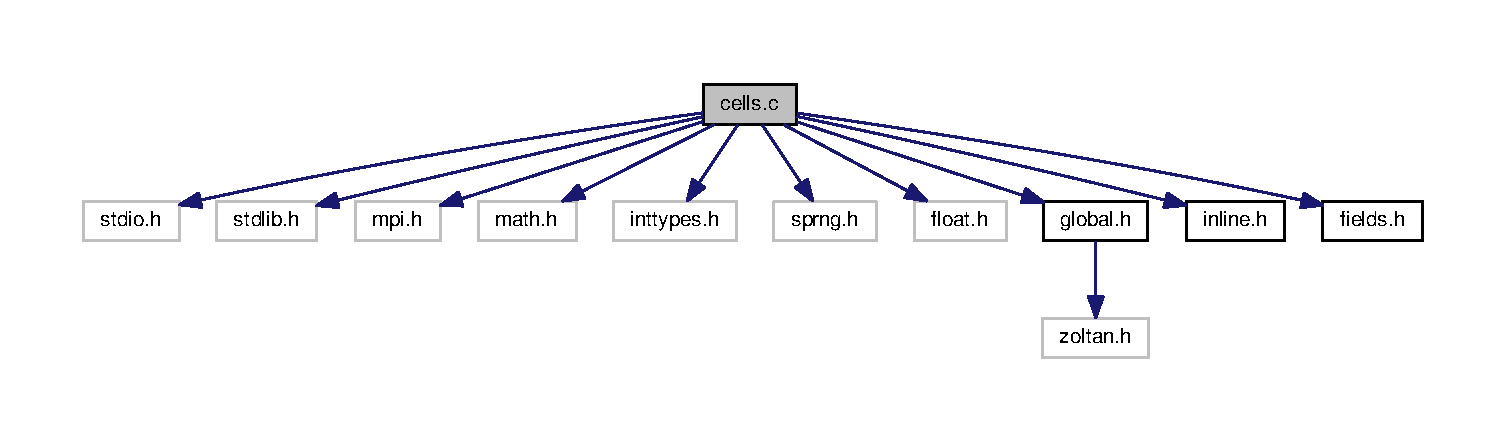
\includegraphics[width=350pt]{cells_8c__incl}
\end{center}
\end{figure}
\subsection*{Functions}
\begin{DoxyCompactItemize}
\item 
void \hyperlink{cells_8c_afdf0714d4b325131b21a0cbe42c44ece}{cells\-Allocate} ()
\item 
void \hyperlink{cells_8c_aa2527c8374034b85c4e95b665786b0ca}{cells\-Cycle\-Init} ()
\item 
int \hyperlink{cells_8c_a68e70197591e819d22315879c8141bdd}{cells\-Random\-Init} ()
\item 
void \hyperlink{cells_8c_a2d9450bd2eebb8f4d645417b92666b87}{mitosis} (int c)
\item 
void \hyperlink{cells_8c_a00dbe1f9f23fc7385462c32b89d28cf8}{mark\-Middle\-Cancer\-Cell} ()
\item 
void \hyperlink{cells_8c_aead37c061c3f1ec47259afaf2783029f}{cells\-Cleanup} ()
\item 
void \hyperlink{cells_8c_a8101c456dae07ab9cbd918ccad3a2ff7}{cells\-Death} (int lnc\-\_\-old)
\item 
void \hyperlink{cells_8c_aeeb6dee9938af6fef987f1c949458703}{update\-Cell\-Counters} ()
\item 
void \hyperlink{cells_8c_af610aeda76899a9384e98f061c317490}{update\-Chemotaxis} ()
\item 
void \hyperlink{cells_8c_a227256c7da11efa2b4eacedf0a9f37c8}{update\-Cell\-Positions} ()
\item 
int \hyperlink{cells_8c_a718a88fce87f8ebdb87ed2fafed4c5c4}{update\-Cell\-Cycles} ()
\item 
void \hyperlink{cells_8c_aa2ee543811c23ee4b487102bb71ba9c7}{additional\-Scalar\-Field} ()
\item 
void \hyperlink{cells_8c_aeb1f066ef0713a8a50eb1e58784a3d7b}{update\-Cell\-States} ()
\end{DoxyCompactItemize}
\subsection*{Variables}
\begin{DoxyCompactItemize}
\item 
unsigned char $\ast$ \hyperlink{cells_8c_a96a825c021fe648b7fb171bd2c532ffb}{celld}
\end{DoxyCompactItemize}


\subsection{Detailed Description}
contains functions which control current states and evolution of cells 

Definition in file \hyperlink{cells_8c_source}{cells.\-c}.



\subsection{Function Documentation}
\hypertarget{cells_8c_aa2ee543811c23ee4b487102bb71ba9c7}{\index{cells.\-c@{cells.\-c}!additional\-Scalar\-Field@{additional\-Scalar\-Field}}
\index{additional\-Scalar\-Field@{additional\-Scalar\-Field}!cells.c@{cells.\-c}}
\subsubsection[{additional\-Scalar\-Field}]{\setlength{\rightskip}{0pt plus 5cm}void additional\-Scalar\-Field (
\begin{DoxyParamCaption}
{}
\end{DoxyParamCaption}
)}}\label{cells_8c_aa2ee543811c23ee4b487102bb71ba9c7}
This function fills the scalar\-Output field of each cell. It can be modified to output any float scalars that user would like to analyze or visualize after simulation. This field is printed to the output V\-T\-K files. 

Definition at line 811 of file cells.\-c.



References cells, cell\-Data\-::density, lnc, and cell\-Data\-::scalar\-Field.


\begin{DoxyCode}
812 \{
813   \textcolor{keywordtype}{int} c;
814   \textcolor{keywordflow}{for} (c = 0; c < \hyperlink{global_8h_a7065c019590815f10169c219f358e7d0}{lnc}; c++) \{
815     \textcolor{keywordflow}{if} (\hyperlink{global_8h_a3ea537bde8d64e54770a2bd81e3f00be}{cells}[c].tumor == 1)
816       \hyperlink{global_8h_a3ea537bde8d64e54770a2bd81e3f00be}{cells}[c].\hyperlink{structcellData_a0045a5036d7f3f873fe33380932d4313}{scalarField} = 8.0;
817     \textcolor{keywordflow}{else}
818       \hyperlink{global_8h_a3ea537bde8d64e54770a2bd81e3f00be}{cells}[c].\hyperlink{structcellData_a0045a5036d7f3f873fe33380932d4313}{scalarField} = \hyperlink{global_8h_a3ea537bde8d64e54770a2bd81e3f00be}{cells}[c].\hyperlink{structcellData_a6f8c052f8417728038991f7f2826d38d}{density};
819   \}
820 \}
\end{DoxyCode}


Here is the caller graph for this function\-:\nopagebreak
\begin{figure}[H]
\begin{center}
\leavevmode
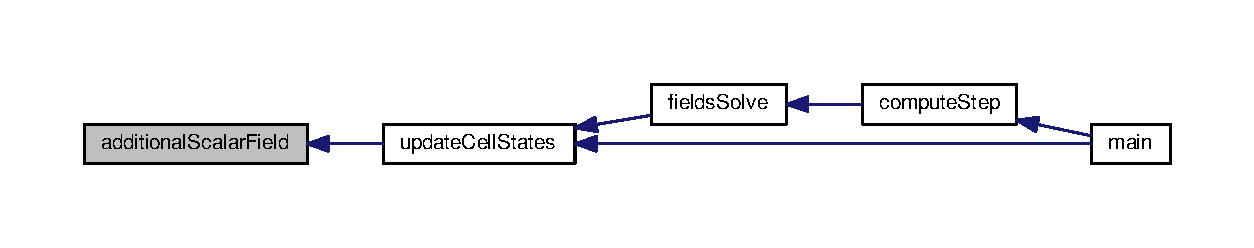
\includegraphics[width=350pt]{cells_8c_aa2ee543811c23ee4b487102bb71ba9c7_icgraph}
\end{center}
\end{figure}


\hypertarget{cells_8c_afdf0714d4b325131b21a0cbe42c44ece}{\index{cells.\-c@{cells.\-c}!cells\-Allocate@{cells\-Allocate}}
\index{cells\-Allocate@{cells\-Allocate}!cells.c@{cells.\-c}}
\subsubsection[{cells\-Allocate}]{\setlength{\rightskip}{0pt plus 5cm}void cells\-Allocate (
\begin{DoxyParamCaption}
{}
\end{DoxyParamCaption}
)}}\label{cells_8c_afdf0714d4b325131b21a0cbe42c44ece}
This function allocates tables responsible for carrying informations about cells, their current state and evolution. 

Definition at line 67 of file cells.\-c.



References cell\-Fields, cells, csize, h, h2, h3, h4, local\-I\-D, max\-Cells, max\-Cells\-Per\-Proc, M\-P\-Isize, N\-C\-H\-E\-M, N\-F\-I\-E\-L\-D\-S, nx, sdim, sim\-Time, stop\-Run(), tlnc, and velocity.


\begin{DoxyCode}
68 \{
69 
70   \textcolor{keywordtype}{int} f;
71   int64\_t cellsActualSize;
72 
73   \textcolor{keywordflow}{if} (\hyperlink{global_8h_a9fad6472ef73b07a138721c11022697a}{sdim} == 2)
74     \hyperlink{global_8h_a39fd0cf73801b603ea78d20e05d8cfd3}{csize} = (\hyperlink{global_8h_a5ff16f483e01fddca329425a21a8b219}{nx} / 2) / pow(8.0 * \hyperlink{global_8h_ac1a3e3adac8f1e6840fd332e3d3cfa21}{maxCells}, 1.0 / 2.0);
75   \textcolor{keywordflow}{if} (\hyperlink{global_8h_a9fad6472ef73b07a138721c11022697a}{sdim} == 3)
76     \hyperlink{global_8h_a39fd0cf73801b603ea78d20e05d8cfd3}{csize} = (\hyperlink{global_8h_a5ff16f483e01fddca329425a21a8b219}{nx} / 2) / pow(8.0 * \hyperlink{global_8h_ac1a3e3adac8f1e6840fd332e3d3cfa21}{maxCells}, 1.0 / 3.0);
77 
78   \hyperlink{global_8h_a2de426dd266cfdaaf6fb52ba3dc2740a}{maxCellsPerProc} = 1.5 * \hyperlink{global_8h_ac1a3e3adac8f1e6840fd332e3d3cfa21}{maxCells} / \hyperlink{global_8h_a0d7d02544d01ceac87c9d5cadc3af0df}{MPIsize};
79 
80   cellsActualSize = \hyperlink{global_8h_a2de426dd266cfdaaf6fb52ba3dc2740a}{maxCellsPerProc} * \textcolor{keyword}{sizeof}(\textcolor{keyword}{struct }\hyperlink{structcellData}{cellData});
81 
82   \hyperlink{global_8h_a265cb7ee626de517ecec0f0ac60833a7}{localID} = 0;
83 
84 \textcolor{preprocessor}{#ifdef \_\_MIC\_\_}
85 \textcolor{preprocessor}{}  \textcolor{keywordflow}{if} (!(\hyperlink{global_8h_a3ea537bde8d64e54770a2bd81e3f00be}{cells} = (\textcolor{keyword}{struct} \hyperlink{structcellData}{cellData} *) \_mm\_malloc(cellsActualSize,64)))
86     \hyperlink{utils_8c_a07dd99a04f2723be164531a7a862fb67}{stopRun}(106, \textcolor{stringliteral}{"cells"}, \_\_FILE\_\_, \_\_LINE\_\_);
87 \textcolor{preprocessor}{#else}
88 \textcolor{preprocessor}{}  \textcolor{keywordflow}{if} (!(\hyperlink{global_8h_a3ea537bde8d64e54770a2bd81e3f00be}{cells} = (\textcolor{keyword}{struct} \hyperlink{structcellData}{cellData} *) malloc(cellsActualSize)))
89     \hyperlink{utils_8c_a07dd99a04f2723be164531a7a862fb67}{stopRun}(106, \textcolor{stringliteral}{"cells"}, \_\_FILE\_\_, \_\_LINE\_\_);
90 \textcolor{preprocessor}{#endif}
91 \textcolor{preprocessor}{}
92 \textcolor{preprocessor}{#ifdef \_\_MIC\_\_}
93 \textcolor{preprocessor}{}  \textcolor{keywordflow}{if} (!(\hyperlink{global_8h_a5ccb3d82df0a6670a0dee2ccd768c0dd}{velocity} = (\textcolor{keyword}{struct} \hyperlink{structdoubleVector3d}{doubleVector3d} *) \_mm\_malloc(
      \hyperlink{global_8h_a2de426dd266cfdaaf6fb52ba3dc2740a}{maxCellsPerProc} *
94                    \textcolor{keyword}{sizeof}(\textcolor{keyword}{struct} \hyperlink{structdoubleVector3d}{doubleVector3d}),64)))
95     \hyperlink{utils_8c_a07dd99a04f2723be164531a7a862fb67}{stopRun}(106, \textcolor{stringliteral}{"velocity"}, \_\_FILE\_\_, \_\_LINE\_\_);
96 \textcolor{preprocessor}{#else}
97 \textcolor{preprocessor}{}  \textcolor{keywordflow}{if} (!(\hyperlink{global_8h_a5ccb3d82df0a6670a0dee2ccd768c0dd}{velocity} = (\textcolor{keyword}{struct} \hyperlink{structdoubleVector3d}{doubleVector3d} *) malloc(
      \hyperlink{global_8h_a2de426dd266cfdaaf6fb52ba3dc2740a}{maxCellsPerProc} *
98                    \textcolor{keyword}{sizeof}(\textcolor{keyword}{struct} \hyperlink{structdoubleVector3d}{doubleVector3d}))))
99     \hyperlink{utils_8c_a07dd99a04f2723be164531a7a862fb67}{stopRun}(106, \textcolor{stringliteral}{"velocity"}, \_\_FILE\_\_, \_\_LINE\_\_);
100 \textcolor{preprocessor}{#endif}
101 \textcolor{preprocessor}{}
102   \hyperlink{global_8h_a25e4317a1b5bb95a8e71e0e8c4e11f2b}{cellFields} = (\textcolor{keywordtype}{double} **) malloc((\hyperlink{fields_8h_a7986f01c038f396ce7df280bb2903099}{NFIELDS}+\hyperlink{fields_8h_af4afd37668ae33da6377a17adff33029}{NCHEM}*3) * \textcolor{keyword}{sizeof}(\textcolor{keywordtype}{double} *));
103   \textcolor{keywordflow}{for} (f = 0; f < \hyperlink{fields_8h_a7986f01c038f396ce7df280bb2903099}{NFIELDS}+\hyperlink{fields_8h_af4afd37668ae33da6377a17adff33029}{NCHEM}*3; f++)
104     \textcolor{keywordflow}{if} (!
105         (\hyperlink{global_8h_a25e4317a1b5bb95a8e71e0e8c4e11f2b}{cellFields}[f] =
106            (\textcolor{keywordtype}{double} *) malloc(\hyperlink{global_8h_a2de426dd266cfdaaf6fb52ba3dc2740a}{maxCellsPerProc} * \textcolor{keyword}{sizeof}(\textcolor{keywordtype}{double}))))
107       \hyperlink{utils_8c_a07dd99a04f2723be164531a7a862fb67}{stopRun}(106, \textcolor{stringliteral}{"cellFields"}, \_\_FILE\_\_, \_\_LINE\_\_);
108 
109   \textcolor{keywordflow}{if} (!(\hyperlink{global_8h_ac3c96b975a3376c555ad22a7d2688b2f}{tlnc} = (int64\_t *) calloc(\hyperlink{global_8h_a0d7d02544d01ceac87c9d5cadc3af0df}{MPIsize}, \textcolor{keyword}{sizeof}(int64\_t))))
110     \hyperlink{utils_8c_a07dd99a04f2723be164531a7a862fb67}{stopRun}(106, \textcolor{stringliteral}{"tlnc"}, \_\_FILE\_\_, \_\_LINE\_\_);
111 
112   \textcolor{comment}{/* cell size */}
113   \textcolor{keywordflow}{if} (\hyperlink{global_8h_a9fad6472ef73b07a138721c11022697a}{sdim} == 2)
114     \hyperlink{global_8h_a39fd0cf73801b603ea78d20e05d8cfd3}{csize} = (\hyperlink{global_8h_a5ff16f483e01fddca329425a21a8b219}{nx} / 2) / pow(8.0 * \hyperlink{global_8h_ac1a3e3adac8f1e6840fd332e3d3cfa21}{maxCells}, 1.0 / 2.0);
115   \textcolor{keywordflow}{if} (\hyperlink{global_8h_a9fad6472ef73b07a138721c11022697a}{sdim} == 3)
116     \hyperlink{global_8h_a39fd0cf73801b603ea78d20e05d8cfd3}{csize} = (\hyperlink{global_8h_a5ff16f483e01fddca329425a21a8b219}{nx} / 2) / pow(8.0 * \hyperlink{global_8h_ac1a3e3adac8f1e6840fd332e3d3cfa21}{maxCells}, 1.0 / 3.0);
117   \hyperlink{global_8h_adae58efd3b7d9072a77aff9c63040d05}{h}=3.0*\hyperlink{global_8h_a39fd0cf73801b603ea78d20e05d8cfd3}{csize};
118   \hyperlink{global_8h_ad188f0f25b4773be09b6eb6babe59f59}{simTime}=0.0;
119   \hyperlink{global_8h_a4c889e0d3615336fbb39aaa8d83bcbc9}{h2} = \hyperlink{global_8h_adae58efd3b7d9072a77aff9c63040d05}{h} * \hyperlink{global_8h_adae58efd3b7d9072a77aff9c63040d05}{h};
120   \hyperlink{global_8h_a15027906d09956cf6cba51d6d24d6769}{h3} = \hyperlink{global_8h_a4c889e0d3615336fbb39aaa8d83bcbc9}{h2} * \hyperlink{global_8h_adae58efd3b7d9072a77aff9c63040d05}{h};
121   \hyperlink{global_8h_a99933cb1baa312807a767a7202baff38}{h4} = \hyperlink{global_8h_a15027906d09956cf6cba51d6d24d6769}{h3} * \hyperlink{global_8h_adae58efd3b7d9072a77aff9c63040d05}{h};
122 
123 
124 \}
\end{DoxyCode}


Here is the call graph for this function\-:\nopagebreak
\begin{figure}[H]
\begin{center}
\leavevmode
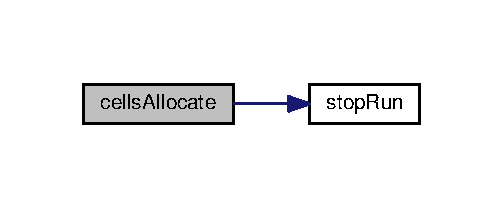
\includegraphics[width=242pt]{cells_8c_afdf0714d4b325131b21a0cbe42c44ece_cgraph}
\end{center}
\end{figure}




Here is the caller graph for this function\-:\nopagebreak
\begin{figure}[H]
\begin{center}
\leavevmode
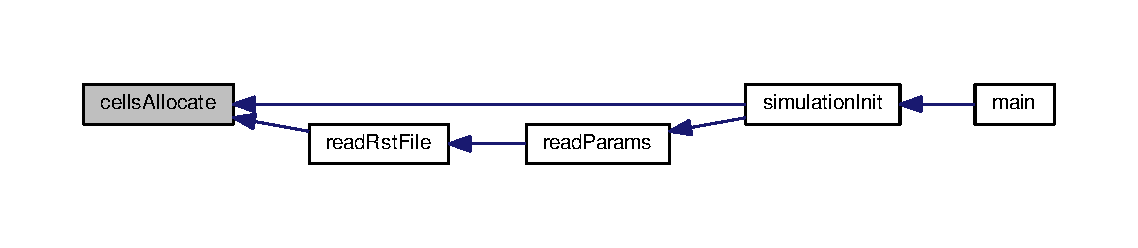
\includegraphics[width=350pt]{cells_8c_afdf0714d4b325131b21a0cbe42c44ece_icgraph}
\end{center}
\end{figure}


\hypertarget{cells_8c_aead37c061c3f1ec47259afaf2783029f}{\index{cells.\-c@{cells.\-c}!cells\-Cleanup@{cells\-Cleanup}}
\index{cells\-Cleanup@{cells\-Cleanup}!cells.c@{cells.\-c}}
\subsubsection[{cells\-Cleanup}]{\setlength{\rightskip}{0pt plus 5cm}void cells\-Cleanup (
\begin{DoxyParamCaption}
{}
\end{DoxyParamCaption}
)}}\label{cells_8c_aead37c061c3f1ec47259afaf2783029f}
This function dealocates all tables allocated during initialization of cell data 

Definition at line 511 of file cells.\-c.



References cell\-Fields, cells, N\-F\-I\-E\-L\-D\-S, tlnc, and velocity.


\begin{DoxyCode}
512 \{
513   \textcolor{keywordtype}{int} f;
514   free(\hyperlink{global_8h_ac3c96b975a3376c555ad22a7d2688b2f}{tlnc});
515 \textcolor{preprocessor}{#ifdef \_\_MIC\_\_}
516 \textcolor{preprocessor}{}  \_mm\_free(\hyperlink{global_8h_a3ea537bde8d64e54770a2bd81e3f00be}{cells});
517 \textcolor{preprocessor}{#else}
518 \textcolor{preprocessor}{}  free(\hyperlink{global_8h_a3ea537bde8d64e54770a2bd81e3f00be}{cells});
519 \textcolor{preprocessor}{#endif}
520 \textcolor{preprocessor}{}  \textcolor{keywordflow}{for} (f = 0; f < \hyperlink{fields_8h_a7986f01c038f396ce7df280bb2903099}{NFIELDS}; f++)
521     free(\hyperlink{global_8h_a25e4317a1b5bb95a8e71e0e8c4e11f2b}{cellFields}[f]);
522   free(\hyperlink{global_8h_a25e4317a1b5bb95a8e71e0e8c4e11f2b}{cellFields});
523 \textcolor{preprocessor}{#ifdef \_\_MIC\_\_}
524 \textcolor{preprocessor}{}  \_mm\_free(\hyperlink{global_8h_a5ccb3d82df0a6670a0dee2ccd768c0dd}{velocity});
525 \textcolor{preprocessor}{#else}
526 \textcolor{preprocessor}{}  free(\hyperlink{global_8h_a5ccb3d82df0a6670a0dee2ccd768c0dd}{velocity});
527 \textcolor{preprocessor}{#endif}
528 \textcolor{preprocessor}{}\}
\end{DoxyCode}


Here is the caller graph for this function\-:\nopagebreak
\begin{figure}[H]
\begin{center}
\leavevmode
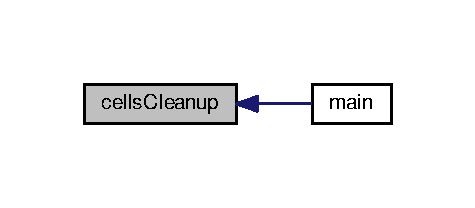
\includegraphics[width=228pt]{cells_8c_aead37c061c3f1ec47259afaf2783029f_icgraph}
\end{center}
\end{figure}


\hypertarget{cells_8c_aa2527c8374034b85c4e95b665786b0ca}{\index{cells.\-c@{cells.\-c}!cells\-Cycle\-Init@{cells\-Cycle\-Init}}
\index{cells\-Cycle\-Init@{cells\-Cycle\-Init}!cells.c@{cells.\-c}}
\subsubsection[{cells\-Cycle\-Init}]{\setlength{\rightskip}{0pt plus 5cm}void cells\-Cycle\-Init (
\begin{DoxyParamCaption}
{}
\end{DoxyParamCaption}
)}}\label{cells_8c_aa2527c8374034b85c4e95b665786b0ca}
This function initializes counters of cells in various cell phases. 

Definition at line 129 of file cells.\-c.



References cancer, cnc, g0nc, g1nc, g2nc, lcnc, lg0nc, lg1nc, lg2nc, lmnc, lnc, lnnc, lsnc, mnc, nc, and snc.


\begin{DoxyCode}
130 \{
131   \textcolor{comment}{/* global numbers of cells */}
132   \hyperlink{global_8h_a33c78f8734fc6805cec2755dd09e0117}{g0nc} = \hyperlink{global_8h_a0845b4b004824f1fe3cd69db1672fa15}{nc};
133   \hyperlink{global_8h_a09b30abbc9cc684e55a246df0528a14b}{g1nc} = 0;
134   \hyperlink{global_8h_a0e24070582e0ecd757fdbdee28c8ff4e}{snc} = 0;
135   \hyperlink{global_8h_ae6288fa86281103b55c317d7f88dca28}{g2nc} = 0;
136   \hyperlink{global_8h_ad1cd19943c182708694e74186fb08015}{mnc} = 0;
137   \hyperlink{global_8h_aec5760e92b3bdf9ac05fc2920446ecd8}{cnc} = 0;
138   \textcolor{comment}{/* local numbers of cells */}
139   \hyperlink{global_8h_a356af225353f2a5512be222c1354bee3}{lg0nc} = \hyperlink{global_8h_a7065c019590815f10169c219f358e7d0}{lnc};
140   \hyperlink{global_8h_a59dc7e07b6be86e29bd0e9f3f18c3ca2}{lg1nc} = 0;
141   \hyperlink{global_8h_af5e326c959f5815222d8f8e3f4d66419}{lsnc} = 0;
142   \hyperlink{global_8h_a17ca9380dca478aa01c68ce4cc8ca720}{lg2nc} = 0;
143   \hyperlink{global_8h_a002cff2ccc4cfc5b5f85ac5ea285ef9c}{lmnc} = 0;
144   \hyperlink{global_8h_ab67f763fa0f30ce2912a6ab60dc8e648}{lcnc} = 0;
145   \hyperlink{global_8h_a97370c479716d79f799616103c487d51}{lnnc} = 0;
146   \textcolor{comment}{/* number of cancer cells */}
147   \hyperlink{global_8h_a543a1902d49aca54ef382bf603a51e27}{cancer} = 0;
148   \textcolor{comment}{/* cell size */}
149   \textcolor{comment}{/*  if (sdim == 2)}
150 \textcolor{comment}{      csize = (nx / 2) / pow(8.0 * maxCells, 1.0 / 2.0);}
151 \textcolor{comment}{    if (sdim == 3)}
152 \textcolor{comment}{      csize = (nx / 2) / pow(8.0 * maxCells, 1.0 / 3.0);}
153 \textcolor{comment}{    h=3.0*csize;}
154 \textcolor{comment}{    simTime=0.0;}
155 \textcolor{comment}{    h2 = h * h;}
156 \textcolor{comment}{    h3 = h2 * h;}
157 \textcolor{comment}{    h4 = h3 * h;}
158 \textcolor{comment}{  */}
159 \}
\end{DoxyCode}


Here is the caller graph for this function\-:\nopagebreak
\begin{figure}[H]
\begin{center}
\leavevmode
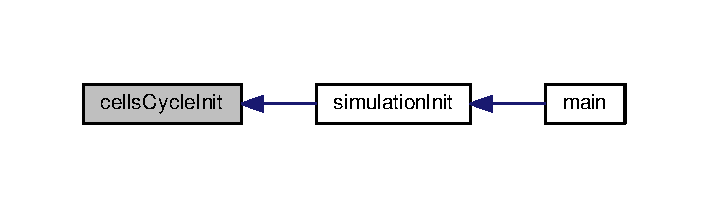
\includegraphics[width=340pt]{cells_8c_aa2527c8374034b85c4e95b665786b0ca_icgraph}
\end{center}
\end{figure}


\hypertarget{cells_8c_a8101c456dae07ab9cbd918ccad3a2ff7}{\index{cells.\-c@{cells.\-c}!cells\-Death@{cells\-Death}}
\index{cells\-Death@{cells\-Death}!cells.c@{cells.\-c}}
\subsubsection[{cells\-Death}]{\setlength{\rightskip}{0pt plus 5cm}void cells\-Death (
\begin{DoxyParamCaption}
\item[{int}]{lnc\-\_\-old}
\end{DoxyParamCaption}
)}}\label{cells_8c_a8101c456dae07ab9cbd918ccad3a2ff7}
This function removes a dead cell from the simulation. 

Definition at line 533 of file cells.\-c.



References celld, cells, lcnc, lg0nc, lg1nc, lg2nc, lmnc, lnc, lsnc, and rsum.


\begin{DoxyCode}
534 \{
535   \textcolor{keywordtype}{int} c, pos;
536 
537   pos = 0;
538   \textcolor{keywordflow}{for} (c = 0; c < \hyperlink{global_8h_a7065c019590815f10169c219f358e7d0}{lnc}; c++) \{
539     \textcolor{comment}{/* shift cells after dead cell removal */}
540     \textcolor{keywordflow}{if} (c >= lnc\_old) \{
541       \hyperlink{global_8h_a3ea537bde8d64e54770a2bd81e3f00be}{cells}[pos] = \hyperlink{global_8h_a3ea537bde8d64e54770a2bd81e3f00be}{cells}[c];
542       pos++;
543       \textcolor{keywordflow}{continue};
544     \}
545     \textcolor{keywordflow}{if} (c != pos && \hyperlink{cells_8c_a96a825c021fe648b7fb171bd2c532ffb}{celld}[c] == 0)
546       \hyperlink{global_8h_a3ea537bde8d64e54770a2bd81e3f00be}{cells}[pos] = \hyperlink{global_8h_a3ea537bde8d64e54770a2bd81e3f00be}{cells}[c];
547     \textcolor{keywordflow}{if} (\hyperlink{cells_8c_a96a825c021fe648b7fb171bd2c532ffb}{celld}[c] == 0)
548       pos++;
549     \textcolor{comment}{/* update cell counters */}
550     \textcolor{keywordflow}{if} (\hyperlink{cells_8c_a96a825c021fe648b7fb171bd2c532ffb}{celld}[c] == 1) \{
551       \textcolor{keywordflow}{switch} (\hyperlink{global_8h_a3ea537bde8d64e54770a2bd81e3f00be}{cells}[c].\hyperlink{structcellData_accf3aec63bc20b3c99ab4881cb07c05b}{phase}) \{
552       \textcolor{keywordflow}{case} 0:
553         \hyperlink{global_8h_a356af225353f2a5512be222c1354bee3}{lg0nc}--;
554         \textcolor{keywordflow}{break};
555       \textcolor{keywordflow}{case} 1:
556         \hyperlink{global_8h_a59dc7e07b6be86e29bd0e9f3f18c3ca2}{lg1nc}--;
557         \textcolor{keywordflow}{break};
558       \textcolor{keywordflow}{case} 2:
559         \hyperlink{global_8h_af5e326c959f5815222d8f8e3f4d66419}{lsnc}--;
560         \textcolor{keywordflow}{break};
561       \textcolor{keywordflow}{case} 3:
562         \hyperlink{global_8h_a17ca9380dca478aa01c68ce4cc8ca720}{lg2nc}--;
563         \textcolor{keywordflow}{break};
564       \textcolor{keywordflow}{case} 4:
565         \hyperlink{global_8h_a002cff2ccc4cfc5b5f85ac5ea285ef9c}{lmnc}--;
566         \textcolor{keywordflow}{break};
567       \}
568       \textcolor{keywordflow}{if} (\hyperlink{global_8h_a3ea537bde8d64e54770a2bd81e3f00be}{cells}[c].\hyperlink{structcellData_a49af8c5336d6c2401bc24f86dbb97b36}{tumor} == 1)
569         \hyperlink{global_8h_ab67f763fa0f30ce2912a6ab60dc8e648}{lcnc}--;
570     \}
571   \}
572   lnc -= \hyperlink{global_8h_a087a95bb36c9b36c708a73ce656fd1f1}{rsum};
573 \}
\end{DoxyCode}


Here is the caller graph for this function\-:\nopagebreak
\begin{figure}[H]
\begin{center}
\leavevmode
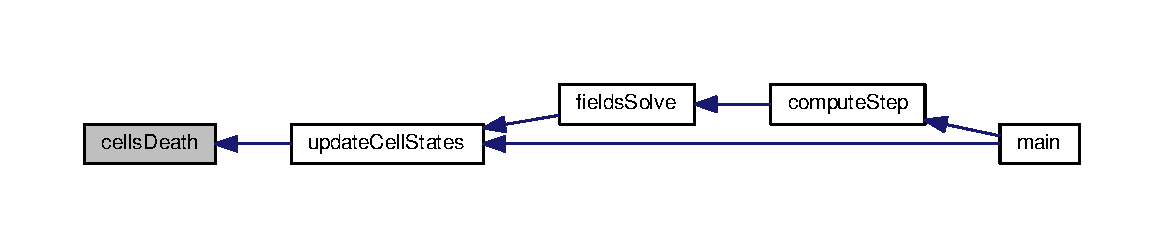
\includegraphics[width=350pt]{cells_8c_a8101c456dae07ab9cbd918ccad3a2ff7_icgraph}
\end{center}
\end{figure}


\hypertarget{cells_8c_a68e70197591e819d22315879c8141bdd}{\index{cells.\-c@{cells.\-c}!cells\-Random\-Init@{cells\-Random\-Init}}
\index{cells\-Random\-Init@{cells\-Random\-Init}!cells.c@{cells.\-c}}
\subsubsection[{cells\-Random\-Init}]{\setlength{\rightskip}{0pt plus 5cm}int cells\-Random\-Init (
\begin{DoxyParamCaption}
{}
\end{DoxyParamCaption}
)}}\label{cells_8c_a68e70197591e819d22315879c8141bdd}
This function initializes cell data. Locations of cells in space are generated randomly. 

Definition at line 165 of file cells.\-c.



References cell\-Data\-::age, bvsim, cells, csize, cell\-Data\-::ctype, cell\-Data\-::death, cell\-Data\-::density, cell\-Data\-::g1, g1, cell\-Data\-::g2, g2, cell\-Data\-::gid, cell\-Data\-::h, h, h2, h3, h4, cell\-Data\-::halo, lbnc, lnc, local\-I\-D, lvc, cell\-Data\-::m, m, max\-Cells, max\-Cells\-Per\-Proc, middle\-Cell\-Idx, M\-P\-Irank, nc, nscinst, nx, cell\-Data\-::phase, cell\-Data\-::phasetime, rng, cell\-Data\-::s, s, cell\-Data\-::scstage, sdim, sim\-Time, cell\-Data\-::size, stream, cell\-Data\-::tumor, cell\-Data\-::v, v, cell\-Data\-::x, cell\-Data\-::y, cell\-Data\-::young, and cell\-Data\-::z.


\begin{DoxyCode}
166 \{
167 
168   \textcolor{keywordtype}{int} i;
169 
170   \textcolor{comment}{/* uniform distribution */}
171   \textcolor{keywordflow}{if} (!strcmp(\hyperlink{global_8h_ae94cd2e37eb46a6942cc45e1b29f87fc}{rng}, \textcolor{stringliteral}{"UNB"})) \{
172     \textcolor{keywordtype}{double} D=1.0;
173 
174     \textcolor{keywordflow}{if} (\hyperlink{global_8h_a9fad6472ef73b07a138721c11022697a}{sdim} == 2)
175       \hyperlink{global_8h_a39fd0cf73801b603ea78d20e05d8cfd3}{csize} = (\hyperlink{global_8h_a5ff16f483e01fddca329425a21a8b219}{nx} / 2) / pow(8.0 * \hyperlink{global_8h_ac1a3e3adac8f1e6840fd332e3d3cfa21}{maxCells}, 1.0 / 2.0);
176     \textcolor{keywordflow}{if} (\hyperlink{global_8h_a9fad6472ef73b07a138721c11022697a}{sdim} == 3)
177       \hyperlink{global_8h_a39fd0cf73801b603ea78d20e05d8cfd3}{csize} = (\hyperlink{global_8h_a5ff16f483e01fddca329425a21a8b219}{nx} / 2) / pow(8.0 * \hyperlink{global_8h_ac1a3e3adac8f1e6840fd332e3d3cfa21}{maxCells}, 1.0 / 3.0);
178     \textcolor{keywordflow}{if} (\hyperlink{global_8h_a9fad6472ef73b07a138721c11022697a}{sdim} == 2)
179       D = \hyperlink{global_8h_a39fd0cf73801b603ea78d20e05d8cfd3}{csize} * pow(8.0 * \hyperlink{global_8h_a0845b4b004824f1fe3cd69db1672fa15}{nc}, 1.0 / 2.0);
180     \textcolor{keywordflow}{if} (\hyperlink{global_8h_a9fad6472ef73b07a138721c11022697a}{sdim} == 3)
181       D = \hyperlink{global_8h_a39fd0cf73801b603ea78d20e05d8cfd3}{csize} * pow(8.0 * \hyperlink{global_8h_a0845b4b004824f1fe3cd69db1672fa15}{nc}, 1.0 / 3.0);
182 
183     \hyperlink{global_8h_adae58efd3b7d9072a77aff9c63040d05}{h} = 3.0 * \hyperlink{global_8h_a39fd0cf73801b603ea78d20e05d8cfd3}{csize};
184     \hyperlink{global_8h_ad188f0f25b4773be09b6eb6babe59f59}{simTime} = 0;
185 
186     \textcolor{keywordflow}{for} (i = 0; i < \hyperlink{global_8h_a7065c019590815f10169c219f358e7d0}{lnc}; i++) \{
187       \hyperlink{global_8h_a3ea537bde8d64e54770a2bd81e3f00be}{cells}[i].\hyperlink{structcellData_af88b946fb90d5f08b5fb740c70e98c10}{x} = D * (sprng(\hyperlink{global_8h_a5340130b6fb2647cef6b71354e27b0d4}{stream}) * 2 - 1);
188       \hyperlink{global_8h_a3ea537bde8d64e54770a2bd81e3f00be}{cells}[i].\hyperlink{structcellData_ab927965981178aa1fba979a37168db2a}{y} = D * (sprng(\hyperlink{global_8h_a5340130b6fb2647cef6b71354e27b0d4}{stream}) * 2 - 1);
189       \textcolor{keywordflow}{if} (\hyperlink{global_8h_a9fad6472ef73b07a138721c11022697a}{sdim} == 3)
190         \hyperlink{global_8h_a3ea537bde8d64e54770a2bd81e3f00be}{cells}[i].\hyperlink{structcellData_ab3e6ed577a7c669c19de1f9c1b46c872}{z} = D * (sprng(\hyperlink{global_8h_a5340130b6fb2647cef6b71354e27b0d4}{stream}) * 2 - 1);
191       \textcolor{keywordflow}{else}
192         \hyperlink{global_8h_a3ea537bde8d64e54770a2bd81e3f00be}{cells}[i].\hyperlink{structcellData_ab3e6ed577a7c669c19de1f9c1b46c872}{z} = 0.0;
193 
194       \hyperlink{global_8h_a3ea537bde8d64e54770a2bd81e3f00be}{cells}[i].\hyperlink{structcellData_af88b946fb90d5f08b5fb740c70e98c10}{x} += \hyperlink{global_8h_a5ff16f483e01fddca329425a21a8b219}{nx} / 2;
195       \hyperlink{global_8h_a3ea537bde8d64e54770a2bd81e3f00be}{cells}[i].\hyperlink{structcellData_ab927965981178aa1fba979a37168db2a}{y} += \hyperlink{global_8h_a5ff16f483e01fddca329425a21a8b219}{nx} / 2;
196       \textcolor{keywordflow}{if} (\hyperlink{global_8h_a9fad6472ef73b07a138721c11022697a}{sdim} == 3)
197         \hyperlink{global_8h_a3ea537bde8d64e54770a2bd81e3f00be}{cells}[i].\hyperlink{structcellData_ab3e6ed577a7c669c19de1f9c1b46c872}{z} += \hyperlink{global_8h_a5ff16f483e01fddca329425a21a8b219}{nx} / 2;
198       \textcolor{keywordflow}{else}
199         \hyperlink{global_8h_a3ea537bde8d64e54770a2bd81e3f00be}{cells}[i].\hyperlink{structcellData_ab3e6ed577a7c669c19de1f9c1b46c872}{z} = 0.0;
200 
201       \hyperlink{global_8h_a3ea537bde8d64e54770a2bd81e3f00be}{cells}[i].\hyperlink{structcellData_aba3c5d750d5dbd6e86c11ecaca62885e}{size} = pow(2.0, -(1.0 / 3.0)) * \hyperlink{global_8h_a39fd0cf73801b603ea78d20e05d8cfd3}{csize};
202       \hyperlink{global_8h_a3ea537bde8d64e54770a2bd81e3f00be}{cells}[i].\hyperlink{structcellData_abb4d4bd9231e9f994e87f32cc4fcfce8}{gid} =
203         (\textcolor{keywordtype}{unsigned} \textcolor{keywordtype}{long} \textcolor{keywordtype}{long} int) \hyperlink{global_8h_a710288ab7d2734acc4566a87a645325d}{MPIrank} *(\textcolor{keywordtype}{unsigned} \textcolor{keywordtype}{long} \textcolor{keywordtype}{long} \textcolor{keywordtype}{int})
204         \hyperlink{global_8h_a2de426dd266cfdaaf6fb52ba3dc2740a}{maxCellsPerProc} + (\textcolor{keywordtype}{unsigned} \textcolor{keywordtype}{long} \textcolor{keywordtype}{long} int) i;
205       \hyperlink{global_8h_a3ea537bde8d64e54770a2bd81e3f00be}{cells}[i].\hyperlink{structcellData_a3b90d5a73541ab9402511d87bed076ef}{v} = 0.0;
206       \hyperlink{global_8h_a3ea537bde8d64e54770a2bd81e3f00be}{cells}[i].\hyperlink{structcellData_a6f8c052f8417728038991f7f2826d38d}{density} = 0.0;
207       \hyperlink{global_8h_a3ea537bde8d64e54770a2bd81e3f00be}{cells}[i].\hyperlink{structcellData_a8ee9be1b5aa75abae556de3088cba6d9}{h} = \hyperlink{global_8h_adae58efd3b7d9072a77aff9c63040d05}{h};
208       \hyperlink{global_8h_a3ea537bde8d64e54770a2bd81e3f00be}{cells}[i].\hyperlink{structcellData_ad0bd87a264e65d1c17ecc07049819f2c}{young} = 2100.0 + sprng(\hyperlink{global_8h_a5340130b6fb2647cef6b71354e27b0d4}{stream}) * 100.0;
209       \hyperlink{global_8h_a3ea537bde8d64e54770a2bd81e3f00be}{cells}[i].\hyperlink{structcellData_a80ff3fcc4d03d0b1b01559839d12df5b}{halo} = 0;
210       \hyperlink{global_8h_a3ea537bde8d64e54770a2bd81e3f00be}{cells}[i].\hyperlink{structcellData_accf3aec63bc20b3c99ab4881cb07c05b}{phase} = 0;
211       \hyperlink{global_8h_a3ea537bde8d64e54770a2bd81e3f00be}{cells}[i].\hyperlink{structcellData_a581debe7d16bce9d187b97855f4e99d4}{g1} = \hyperlink{global_8h_a581debe7d16bce9d187b97855f4e99d4}{g1} * (1 + (sprng(\hyperlink{global_8h_a5340130b6fb2647cef6b71354e27b0d4}{stream}) * 2 - 1) * \hyperlink{global_8h_a48d9522e58fa05906c6dba23e5745a72}{v});
212       \hyperlink{global_8h_a3ea537bde8d64e54770a2bd81e3f00be}{cells}[i].\hyperlink{structcellData_aee9971139118d56815564304450c4775}{g2} = \hyperlink{global_8h_aee9971139118d56815564304450c4775}{g2} * (1 + (sprng(\hyperlink{global_8h_a5340130b6fb2647cef6b71354e27b0d4}{stream}) * 2 - 1) * \hyperlink{global_8h_a48d9522e58fa05906c6dba23e5745a72}{v});
213       \hyperlink{global_8h_a3ea537bde8d64e54770a2bd81e3f00be}{cells}[i].\hyperlink{structcellData_a874f74a4dc1c9a0cd9c6e0d79c298f55}{s} = \hyperlink{global_8h_a874f74a4dc1c9a0cd9c6e0d79c298f55}{s} * (1 + (sprng(\hyperlink{global_8h_a5340130b6fb2647cef6b71354e27b0d4}{stream}) * 2 - 1) * \hyperlink{global_8h_a48d9522e58fa05906c6dba23e5745a72}{v});
214       \hyperlink{global_8h_a3ea537bde8d64e54770a2bd81e3f00be}{cells}[i].\hyperlink{structcellData_ac51334f57ef8b81c0629c9421798c344}{m} = \hyperlink{global_8h_ac51334f57ef8b81c0629c9421798c344}{m} * (1 + (sprng(\hyperlink{global_8h_a5340130b6fb2647cef6b71354e27b0d4}{stream}) * 2 - 1) * \hyperlink{global_8h_a48d9522e58fa05906c6dba23e5745a72}{v});
215       \hyperlink{global_8h_a3ea537bde8d64e54770a2bd81e3f00be}{cells}[i].\hyperlink{structcellData_afe1297f954440c453b59fcb06992dbd5}{phasetime} = 0.0;
216       \hyperlink{global_8h_a3ea537bde8d64e54770a2bd81e3f00be}{cells}[i].\hyperlink{structcellData_a91d98a856bbd96810b40af3ca5cc901a}{age} = 0;
217       \hyperlink{global_8h_a3ea537bde8d64e54770a2bd81e3f00be}{cells}[i].\hyperlink{structcellData_add1e1533be6e693ffedcdbafdf8b855c}{death} = 0;
218       \hyperlink{global_8h_a3ea537bde8d64e54770a2bd81e3f00be}{cells}[i].\hyperlink{structcellData_a49af8c5336d6c2401bc24f86dbb97b36}{tumor} = 0;
219       \hyperlink{global_8h_a3ea537bde8d64e54770a2bd81e3f00be}{cells}[i].\hyperlink{structcellData_a13fbf3c17594503f639a7ef768ea73bb}{ctype} = 0;
220       \hyperlink{global_8h_a3ea537bde8d64e54770a2bd81e3f00be}{cells}[i].\hyperlink{structcellData_addbb21027771706513a66fdf00c123f3}{scstage} = 0;
221       \hyperlink{global_8h_a265cb7ee626de517ecec0f0ac60833a7}{localID}++;
222     \}
223     \hyperlink{global_8h_a1d0cb64baa35f225f63d7e205a36d530}{nscinst}[0]+=\hyperlink{global_8h_a7065c019590815f10169c219f358e7d0}{lnc};
224   \}
225   \textcolor{comment}{/* normal distribution (Box-Muller transform) */}
226   \textcolor{keywordflow}{if} (!strcmp(\hyperlink{global_8h_ae94cd2e37eb46a6942cc45e1b29f87fc}{rng}, \textcolor{stringliteral}{"BM"})) \{
227     \textcolor{keywordtype}{double} x1, x2, x3;
228     \textcolor{keywordtype}{double} z1, z2, z3;
229     \textcolor{keywordtype}{double} r1, r2;
230     \textcolor{keywordtype}{double} l;
231     \textcolor{keywordtype}{double} D=1.0;
232     \textcolor{keywordflow}{if} (\hyperlink{global_8h_a9fad6472ef73b07a138721c11022697a}{sdim} == 2)
233       \hyperlink{global_8h_a39fd0cf73801b603ea78d20e05d8cfd3}{csize} = (\hyperlink{global_8h_a5ff16f483e01fddca329425a21a8b219}{nx} / 2) / pow(8.0 * \hyperlink{global_8h_ac1a3e3adac8f1e6840fd332e3d3cfa21}{maxCells}, 1.0 / 2.0);
234     \textcolor{keywordflow}{if} (\hyperlink{global_8h_a9fad6472ef73b07a138721c11022697a}{sdim} == 3)
235       \hyperlink{global_8h_a39fd0cf73801b603ea78d20e05d8cfd3}{csize} = (\hyperlink{global_8h_a5ff16f483e01fddca329425a21a8b219}{nx} / 2) / pow(8.0 * \hyperlink{global_8h_ac1a3e3adac8f1e6840fd332e3d3cfa21}{maxCells}, 1.0 / 3.0);
236     \textcolor{keywordflow}{if} (\hyperlink{global_8h_a9fad6472ef73b07a138721c11022697a}{sdim} == 2)
237       D = \hyperlink{global_8h_a39fd0cf73801b603ea78d20e05d8cfd3}{csize} * pow(8.0 * \hyperlink{global_8h_a0845b4b004824f1fe3cd69db1672fa15}{nc}, 1.0 / 2.0);
238     \textcolor{keywordflow}{if} (\hyperlink{global_8h_a9fad6472ef73b07a138721c11022697a}{sdim} == 3)
239       D = \hyperlink{global_8h_a39fd0cf73801b603ea78d20e05d8cfd3}{csize} * pow(8.0 * \hyperlink{global_8h_a0845b4b004824f1fe3cd69db1672fa15}{nc}, 1.0 / 3.0);
240 
241     \hyperlink{global_8h_adae58efd3b7d9072a77aff9c63040d05}{h} = 3.0 * \hyperlink{global_8h_a39fd0cf73801b603ea78d20e05d8cfd3}{csize};
242     \hyperlink{global_8h_ad188f0f25b4773be09b6eb6babe59f59}{simTime} = 0;
243     \textcolor{keywordflow}{for} (i = 0; i < \hyperlink{global_8h_a7065c019590815f10169c219f358e7d0}{lnc}-\hyperlink{global_8h_a54901de38c37cfcd038a1e723cd4ecb8}{lvc}-\hyperlink{global_8h_a0cb9f3a12f8c024f27273125d2f07efb}{lbnc}; i++) \{
244 
245       r2 = 1.1;
246 
247       \textcolor{keywordflow}{while} (r2 >= 1.0) \{
248         r1 = 1.1;
249         \textcolor{keywordflow}{while} (r1 == 0 || r1 >= 1.0) \{
250           x1 = sprng(\hyperlink{global_8h_a5340130b6fb2647cef6b71354e27b0d4}{stream}) * 2 - 1;
251           x2 = sprng(\hyperlink{global_8h_a5340130b6fb2647cef6b71354e27b0d4}{stream}) * 2 - 1;
252           x3 = sprng(\hyperlink{global_8h_a5340130b6fb2647cef6b71354e27b0d4}{stream}) * 2 - 1;
253           r1 = x1 * x1 + x2 * x2 + x3 * x3;
254         \}
255         l = sqrt(-2 * log(r1) / r1);
256         z1 = x1 * l;
257         z2 = x2 * l;
258         z3 = x3 * l;
259 
260         r2 = z1 * z1 + z2 * z2 + z3 * z3;
261       \}
262 
263       \textcolor{keywordflow}{if}(\hyperlink{global_8h_a975a504c34469eed96d609d621cfa35a}{bvsim}) \{
264         \hyperlink{global_8h_a3ea537bde8d64e54770a2bd81e3f00be}{cells}[i].\hyperlink{structcellData_af88b946fb90d5f08b5fb740c70e98c10}{x}=\hyperlink{global_8h_a3ea537bde8d64e54770a2bd81e3f00be}{cells}[\hyperlink{global_8h_aba24a5782ec50a3e3febdf4ce2b567d4}{middleCellIdx}].\hyperlink{structcellData_af88b946fb90d5f08b5fb740c70e98c10}{x}-0.8;
265         \hyperlink{global_8h_a3ea537bde8d64e54770a2bd81e3f00be}{cells}[i].\hyperlink{structcellData_ab927965981178aa1fba979a37168db2a}{y}=\hyperlink{global_8h_a3ea537bde8d64e54770a2bd81e3f00be}{cells}[\hyperlink{global_8h_aba24a5782ec50a3e3febdf4ce2b567d4}{middleCellIdx}].\hyperlink{structcellData_ab927965981178aa1fba979a37168db2a}{y}-0.8;
266         \hyperlink{global_8h_a3ea537bde8d64e54770a2bd81e3f00be}{cells}[i].\hyperlink{structcellData_ab3e6ed577a7c669c19de1f9c1b46c872}{z}=\hyperlink{global_8h_a3ea537bde8d64e54770a2bd81e3f00be}{cells}[\hyperlink{global_8h_aba24a5782ec50a3e3febdf4ce2b567d4}{middleCellIdx}].\hyperlink{structcellData_ab3e6ed577a7c669c19de1f9c1b46c872}{z}+0.01;
267       \} \textcolor{keywordflow}{else} \{
268         \hyperlink{global_8h_a3ea537bde8d64e54770a2bd81e3f00be}{cells}[i].\hyperlink{structcellData_af88b946fb90d5f08b5fb740c70e98c10}{x} = z1 * D + \hyperlink{global_8h_a5ff16f483e01fddca329425a21a8b219}{nx} / 2;
269         \hyperlink{global_8h_a3ea537bde8d64e54770a2bd81e3f00be}{cells}[i].\hyperlink{structcellData_ab927965981178aa1fba979a37168db2a}{y} = z2 * D + \hyperlink{global_8h_a5ff16f483e01fddca329425a21a8b219}{nx} / 2;
270         \textcolor{keywordflow}{if} (\hyperlink{global_8h_a9fad6472ef73b07a138721c11022697a}{sdim} == 3)
271           \hyperlink{global_8h_a3ea537bde8d64e54770a2bd81e3f00be}{cells}[i].\hyperlink{structcellData_ab3e6ed577a7c669c19de1f9c1b46c872}{z} = z3 * D + \hyperlink{global_8h_a5ff16f483e01fddca329425a21a8b219}{nx} / 2;
272         \textcolor{keywordflow}{else}
273           \hyperlink{global_8h_a3ea537bde8d64e54770a2bd81e3f00be}{cells}[i].\hyperlink{structcellData_ab3e6ed577a7c669c19de1f9c1b46c872}{z} = 0.0;
274       \}
275 
276       \hyperlink{global_8h_a3ea537bde8d64e54770a2bd81e3f00be}{cells}[i].\hyperlink{structcellData_aba3c5d750d5dbd6e86c11ecaca62885e}{size} = pow(2.0, -(1.0 / 3.0)) * \hyperlink{global_8h_a39fd0cf73801b603ea78d20e05d8cfd3}{csize};
277       \hyperlink{global_8h_a3ea537bde8d64e54770a2bd81e3f00be}{cells}[i].\hyperlink{structcellData_abb4d4bd9231e9f994e87f32cc4fcfce8}{gid} =
278         (\textcolor{keywordtype}{unsigned} \textcolor{keywordtype}{long} \textcolor{keywordtype}{long} int) \hyperlink{global_8h_a710288ab7d2734acc4566a87a645325d}{MPIrank} *(\textcolor{keywordtype}{unsigned} \textcolor{keywordtype}{long} \textcolor{keywordtype}{long} \textcolor{keywordtype}{int})
279         \hyperlink{global_8h_a2de426dd266cfdaaf6fb52ba3dc2740a}{maxCellsPerProc} + (\textcolor{keywordtype}{unsigned} \textcolor{keywordtype}{long} \textcolor{keywordtype}{long} int) i;
280       \hyperlink{global_8h_a3ea537bde8d64e54770a2bd81e3f00be}{cells}[i].\hyperlink{structcellData_a3b90d5a73541ab9402511d87bed076ef}{v} = 0.0;
281       \hyperlink{global_8h_a3ea537bde8d64e54770a2bd81e3f00be}{cells}[i].\hyperlink{structcellData_a6f8c052f8417728038991f7f2826d38d}{density} = 0.0;
282       \hyperlink{global_8h_a3ea537bde8d64e54770a2bd81e3f00be}{cells}[i].\hyperlink{structcellData_a8ee9be1b5aa75abae556de3088cba6d9}{h} = \hyperlink{global_8h_adae58efd3b7d9072a77aff9c63040d05}{h};
283       \hyperlink{global_8h_a3ea537bde8d64e54770a2bd81e3f00be}{cells}[i].\hyperlink{structcellData_ad0bd87a264e65d1c17ecc07049819f2c}{young} = 2100.0 + sprng(\hyperlink{global_8h_a5340130b6fb2647cef6b71354e27b0d4}{stream}) * 100.0;
284       \hyperlink{global_8h_a3ea537bde8d64e54770a2bd81e3f00be}{cells}[i].\hyperlink{structcellData_a80ff3fcc4d03d0b1b01559839d12df5b}{halo} = 0;
285       \hyperlink{global_8h_a3ea537bde8d64e54770a2bd81e3f00be}{cells}[i].\hyperlink{structcellData_accf3aec63bc20b3c99ab4881cb07c05b}{phase} = 0;
286       \hyperlink{global_8h_a3ea537bde8d64e54770a2bd81e3f00be}{cells}[i].\hyperlink{structcellData_a581debe7d16bce9d187b97855f4e99d4}{g1} = \hyperlink{global_8h_a581debe7d16bce9d187b97855f4e99d4}{g1} * (1 + (sprng(\hyperlink{global_8h_a5340130b6fb2647cef6b71354e27b0d4}{stream}) * 2 - 1) * \hyperlink{global_8h_a48d9522e58fa05906c6dba23e5745a72}{v});
287       \hyperlink{global_8h_a3ea537bde8d64e54770a2bd81e3f00be}{cells}[i].\hyperlink{structcellData_aee9971139118d56815564304450c4775}{g2} = \hyperlink{global_8h_aee9971139118d56815564304450c4775}{g2} * (1 + (sprng(\hyperlink{global_8h_a5340130b6fb2647cef6b71354e27b0d4}{stream}) * 2 - 1) * \hyperlink{global_8h_a48d9522e58fa05906c6dba23e5745a72}{v});
288       \hyperlink{global_8h_a3ea537bde8d64e54770a2bd81e3f00be}{cells}[i].\hyperlink{structcellData_a874f74a4dc1c9a0cd9c6e0d79c298f55}{s} = \hyperlink{global_8h_a874f74a4dc1c9a0cd9c6e0d79c298f55}{s} * (1 + (sprng(\hyperlink{global_8h_a5340130b6fb2647cef6b71354e27b0d4}{stream}) * 2 - 1) * \hyperlink{global_8h_a48d9522e58fa05906c6dba23e5745a72}{v});
289       \hyperlink{global_8h_a3ea537bde8d64e54770a2bd81e3f00be}{cells}[i].\hyperlink{structcellData_ac51334f57ef8b81c0629c9421798c344}{m} = \hyperlink{global_8h_ac51334f57ef8b81c0629c9421798c344}{m} * (1 + (sprng(\hyperlink{global_8h_a5340130b6fb2647cef6b71354e27b0d4}{stream}) * 2 - 1) * \hyperlink{global_8h_a48d9522e58fa05906c6dba23e5745a72}{v});
290       \hyperlink{global_8h_a3ea537bde8d64e54770a2bd81e3f00be}{cells}[i].\hyperlink{structcellData_afe1297f954440c453b59fcb06992dbd5}{phasetime} = 0.0;
291       \hyperlink{global_8h_a3ea537bde8d64e54770a2bd81e3f00be}{cells}[i].\hyperlink{structcellData_a49af8c5336d6c2401bc24f86dbb97b36}{tumor} = 0;
292       \hyperlink{global_8h_a3ea537bde8d64e54770a2bd81e3f00be}{cells}[i].\hyperlink{structcellData_a91d98a856bbd96810b40af3ca5cc901a}{age} = 0;
293       \hyperlink{global_8h_a3ea537bde8d64e54770a2bd81e3f00be}{cells}[i].\hyperlink{structcellData_add1e1533be6e693ffedcdbafdf8b855c}{death} = 0;
294       \hyperlink{global_8h_a3ea537bde8d64e54770a2bd81e3f00be}{cells}[i].\hyperlink{structcellData_a13fbf3c17594503f639a7ef768ea73bb}{ctype} = 0;
295       \hyperlink{global_8h_a3ea537bde8d64e54770a2bd81e3f00be}{cells}[i].\hyperlink{structcellData_addbb21027771706513a66fdf00c123f3}{scstage} = 0;
296       \hyperlink{global_8h_a265cb7ee626de517ecec0f0ac60833a7}{localID}++;
297     \}
298   \}
299 
300   \hyperlink{global_8h_a1d0cb64baa35f225f63d7e205a36d530}{nscinst}[0]+=\hyperlink{global_8h_a7065c019590815f10169c219f358e7d0}{lnc};
301 
302   \textcolor{comment}{/* powers of h are calculated only once here */}
303   \hyperlink{global_8h_a4c889e0d3615336fbb39aaa8d83bcbc9}{h2} = \hyperlink{global_8h_adae58efd3b7d9072a77aff9c63040d05}{h} * \hyperlink{global_8h_adae58efd3b7d9072a77aff9c63040d05}{h};
304   \hyperlink{global_8h_a15027906d09956cf6cba51d6d24d6769}{h3} = \hyperlink{global_8h_a4c889e0d3615336fbb39aaa8d83bcbc9}{h2} * \hyperlink{global_8h_adae58efd3b7d9072a77aff9c63040d05}{h};
305   \hyperlink{global_8h_a99933cb1baa312807a767a7202baff38}{h4} = \hyperlink{global_8h_a15027906d09956cf6cba51d6d24d6769}{h3} * \hyperlink{global_8h_adae58efd3b7d9072a77aff9c63040d05}{h};
306 
307   \textcolor{keywordflow}{return} 0;
308 \}
\end{DoxyCode}


Here is the caller graph for this function\-:\nopagebreak
\begin{figure}[H]
\begin{center}
\leavevmode
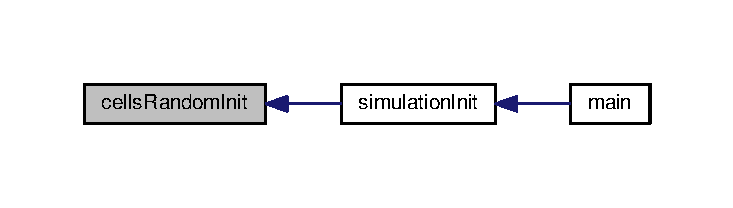
\includegraphics[width=350pt]{cells_8c_a68e70197591e819d22315879c8141bdd_icgraph}
\end{center}
\end{figure}


\hypertarget{cells_8c_a00dbe1f9f23fc7385462c32b89d28cf8}{\index{cells.\-c@{cells.\-c}!mark\-Middle\-Cancer\-Cell@{mark\-Middle\-Cancer\-Cell}}
\index{mark\-Middle\-Cancer\-Cell@{mark\-Middle\-Cancer\-Cell}!cells.c@{cells.\-c}}
\subsubsection[{mark\-Middle\-Cancer\-Cell}]{\setlength{\rightskip}{0pt plus 5cm}void mark\-Middle\-Cancer\-Cell (
\begin{DoxyParamCaption}
{}
\end{DoxyParamCaption}
)}}\label{cells_8c_a00dbe1f9f23fc7385462c32b89d28cf8}
This function finds locates cell closest to the center of mass of the system and marks this cell as a cancer cell. 

Definition at line 451 of file cells.\-c.



References cancer, cells, lcnc, lg0nc, lg1nc, lnc, M\-P\-Irank, nc, cell\-Data\-::phase, cell\-Data\-::tumor, x, cell\-Data\-::x, cell\-Data\-::y, and cell\-Data\-::z.


\begin{DoxyCode}
452 \{
453   \textcolor{keywordtype}{int} c;
454   \textcolor{keywordtype}{int} middle = 0;
455   \textcolor{keywordtype}{double} dist;
456   \textcolor{keyword}{struct }\{
457     \textcolor{keywordtype}{double} val;
458     \textcolor{keywordtype}{int} rank;
459   \} lmdist, gmdist;
460   \textcolor{keywordtype}{double} center[3];
461   \textcolor{keywordtype}{double} gcenter[3];
462 
463   \textcolor{comment}{/* each process computes its local center of mass */}
464   center[0] = 0.0;
465   center[1] = 0.0;
466   center[2] = 0.0;
467   \textcolor{keywordflow}{for} (c = 0; c < \hyperlink{global_8h_a7065c019590815f10169c219f358e7d0}{lnc}; c++) \{
468     center[0] += \hyperlink{global_8h_a3ea537bde8d64e54770a2bd81e3f00be}{cells}[c].\hyperlink{structcellData_af88b946fb90d5f08b5fb740c70e98c10}{x} / \hyperlink{global_8h_a0845b4b004824f1fe3cd69db1672fa15}{nc};
469     center[1] += \hyperlink{global_8h_a3ea537bde8d64e54770a2bd81e3f00be}{cells}[c].\hyperlink{structcellData_ab927965981178aa1fba979a37168db2a}{y} / \hyperlink{global_8h_a0845b4b004824f1fe3cd69db1672fa15}{nc};
470     center[2] += \hyperlink{global_8h_a3ea537bde8d64e54770a2bd81e3f00be}{cells}[c].\hyperlink{structcellData_ab3e6ed577a7c669c19de1f9c1b46c872}{z} / \hyperlink{global_8h_a0845b4b004824f1fe3cd69db1672fa15}{nc};
471   \}
472 
473   \textcolor{comment}{/* MPI Reduce operation computes global center of mass */}
474   MPI\_Allreduce(center, gcenter, 3, MPI\_DOUBLE, MPI\_SUM, MPI\_COMM\_WORLD);
475 
476   \textcolor{comment}{/* intialization */}
477   lmdist.rank = \hyperlink{global_8h_a710288ab7d2734acc4566a87a645325d}{MPIrank};
478   lmdist.val = INT\_MAX;
479 
480   \textcolor{comment}{/* each process finds local cell closest to the global center of mass */}
481   \textcolor{keywordflow}{for} (c = 0; c < \hyperlink{global_8h_a7065c019590815f10169c219f358e7d0}{lnc}; c++) \{
482     dist =
483       sqrt((\hyperlink{global_8h_a3ea537bde8d64e54770a2bd81e3f00be}{cells}[c].\hyperlink{tempf_8c_a1780e9c70637026d6fab31f63b3a193e}{x} - gcenter[0]) * (\hyperlink{global_8h_a3ea537bde8d64e54770a2bd81e3f00be}{cells}[c].\hyperlink{tempf_8c_a1780e9c70637026d6fab31f63b3a193e}{x} - gcenter[0]) +
484            (\hyperlink{global_8h_a3ea537bde8d64e54770a2bd81e3f00be}{cells}[c].y - gcenter[1]) * (\hyperlink{global_8h_a3ea537bde8d64e54770a2bd81e3f00be}{cells}[c].y - gcenter[1]) +
485            (\hyperlink{global_8h_a3ea537bde8d64e54770a2bd81e3f00be}{cells}[c].z - gcenter[2]) * (\hyperlink{global_8h_a3ea537bde8d64e54770a2bd81e3f00be}{cells}[c].z - gcenter[2]));
486     \textcolor{keywordflow}{if} (dist < lmdist.val) \{
487       lmdist.val = dist;
488       middle = c;
489     \}
490   \}
491 
492   \textcolor{comment}{/* MPI\_Allreduce locates the cell closest to the global center of mass */}
493   MPI\_Allreduce(&lmdist, &gmdist, 1, MPI\_DOUBLE\_INT, MPI\_MINLOC,
494                 MPI\_COMM\_WORLD);
495   \textcolor{comment}{/* mark the found cell as cancer one */}
496   \textcolor{keywordflow}{if} (\hyperlink{global_8h_a710288ab7d2734acc4566a87a645325d}{MPIrank} == gmdist.rank) \{
497     \hyperlink{global_8h_a3ea537bde8d64e54770a2bd81e3f00be}{cells}[middle].\hyperlink{structcellData_a49af8c5336d6c2401bc24f86dbb97b36}{tumor} = 1;
498     \hyperlink{global_8h_a3ea537bde8d64e54770a2bd81e3f00be}{cells}[middle].\hyperlink{structcellData_accf3aec63bc20b3c99ab4881cb07c05b}{phase} = 1;
499     \hyperlink{global_8h_a356af225353f2a5512be222c1354bee3}{lg0nc}--;
500     \hyperlink{global_8h_a59dc7e07b6be86e29bd0e9f3f18c3ca2}{lg1nc}++;
501     \hyperlink{global_8h_ab67f763fa0f30ce2912a6ab60dc8e648}{lcnc}++;
502   \}
503 
504   \textcolor{comment}{/* indicate that there is a cancer cell in the system */}
505   \hyperlink{global_8h_a543a1902d49aca54ef382bf603a51e27}{cancer} = 1;
506 \}
\end{DoxyCode}


Here is the caller graph for this function\-:\nopagebreak
\begin{figure}[H]
\begin{center}
\leavevmode
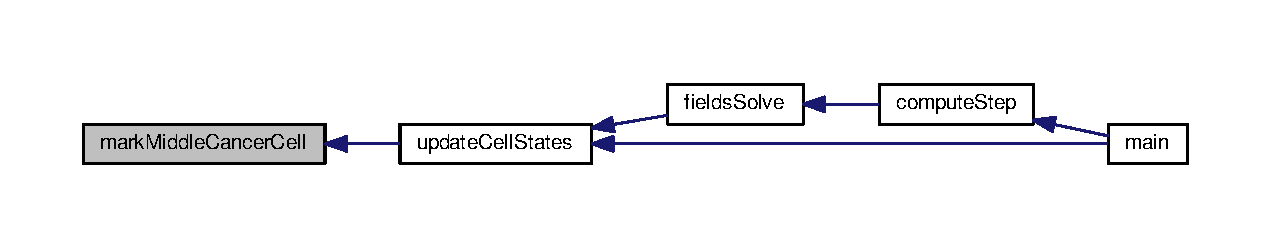
\includegraphics[width=350pt]{cells_8c_a00dbe1f9f23fc7385462c32b89d28cf8_icgraph}
\end{center}
\end{figure}


\hypertarget{cells_8c_a2d9450bd2eebb8f4d645417b92666b87}{\index{cells.\-c@{cells.\-c}!mitosis@{mitosis}}
\index{mitosis@{mitosis}!cells.c@{cells.\-c}}
\subsubsection[{mitosis}]{\setlength{\rightskip}{0pt plus 5cm}void mitosis (
\begin{DoxyParamCaption}
\item[{int}]{c}
\end{DoxyParamCaption}
)}}\label{cells_8c_a2d9450bd2eebb8f4d645417b92666b87}
This function implements mitosis of cells. 

Definition at line 313 of file cells.\-c.



References cell\-Data\-::age, celld, cells, cg1, cg2, cm, cs, cell\-Data\-::death, cell\-Data\-::density, cell\-Data\-::g1, g1, cell\-Data\-::g2, g2, cell\-Data\-::gid, cell\-Data\-::h, h, cell\-Data\-::halo, lcnc, lg1nc, lnc, localbc, local\-I\-D, cell\-Data\-::m, m, max\-Cells\-Per\-Proc, mitrand, M\-P\-Irank, nscinst, nscstages, cell\-Data\-::phase, cell\-Data\-::phasetime, cell\-Data\-::s, s, cell\-Data\-::scstage, sctprob, sdim, cell\-Data\-::size, stop\-Run(), stream, cell\-Data\-::tumor, cell\-Data\-::v, v, velocity, x, cell\-Data\-::x, double\-Vector3d\-::x, cell\-Data\-::y, double\-Vector3d\-::y, cell\-Data\-::young, cell\-Data\-::z, and double\-Vector3d\-::z.


\begin{DoxyCode}
314 \{
315 
316   \textcolor{keywordtype}{double} sc;
317   \textcolor{keywordtype}{double} shift[3];
318 
319   \textcolor{keywordflow}{if} (\hyperlink{global_8h_a7065c019590815f10169c219f358e7d0}{lnc} + 1 > \hyperlink{global_8h_a2de426dd266cfdaaf6fb52ba3dc2740a}{maxCellsPerProc})
320     \hyperlink{utils_8c_a07dd99a04f2723be164531a7a862fb67}{stopRun}(109, NULL, \_\_FILE\_\_, \_\_LINE\_\_);
321 
322   \textcolor{comment}{/* stem cells counters */}
323   \textcolor{keywordflow}{if}(\hyperlink{global_8h_a3ea537bde8d64e54770a2bd81e3f00be}{cells}[c].scstage==\hyperlink{global_8h_a612536506e4e3cb48d8e88b795c8beed}{nscstages}-1) \{
324     \textcolor{keywordflow}{if}(sprng(\hyperlink{global_8h_a5340130b6fb2647cef6b71354e27b0d4}{stream})>\hyperlink{global_8h_a76e4f96985235f18bbf5cccc2608c430}{sctprob}[\hyperlink{global_8h_a3ea537bde8d64e54770a2bd81e3f00be}{cells}[c].scstage]) \{
325       \hyperlink{cells_8c_a96a825c021fe648b7fb171bd2c532ffb}{celld}[c]=1;
326       \hyperlink{global_8h_acffece8fb8e971c4a430ae58e28c4980}{localbc}+=1;
327     \}
328     \textcolor{keywordflow}{return};
329   \}
330 
331   \textcolor{keywordflow}{if}(\hyperlink{global_8h_a3ea537bde8d64e54770a2bd81e3f00be}{cells}[c].scstage<\hyperlink{global_8h_a612536506e4e3cb48d8e88b795c8beed}{nscstages}-1) \{
332     \textcolor{keywordflow}{if}(sprng(\hyperlink{global_8h_a5340130b6fb2647cef6b71354e27b0d4}{stream})>\hyperlink{global_8h_a76e4f96985235f18bbf5cccc2608c430}{sctprob}[\hyperlink{global_8h_a3ea537bde8d64e54770a2bd81e3f00be}{cells}[c].scstage]) \{
333       \hyperlink{global_8h_a3ea537bde8d64e54770a2bd81e3f00be}{cells}[\hyperlink{global_8h_a7065c019590815f10169c219f358e7d0}{lnc}].\hyperlink{structcellData_addbb21027771706513a66fdf00c123f3}{scstage}=\hyperlink{global_8h_a3ea537bde8d64e54770a2bd81e3f00be}{cells}[c].\hyperlink{structcellData_addbb21027771706513a66fdf00c123f3}{scstage}+1;
334       \hyperlink{global_8h_a1d0cb64baa35f225f63d7e205a36d530}{nscinst}[\hyperlink{global_8h_a3ea537bde8d64e54770a2bd81e3f00be}{cells}[\hyperlink{global_8h_a7065c019590815f10169c219f358e7d0}{lnc}].\hyperlink{structcellData_addbb21027771706513a66fdf00c123f3}{scstage}]+=1;
335     \} \textcolor{keywordflow}{else} \{
336       \hyperlink{global_8h_a3ea537bde8d64e54770a2bd81e3f00be}{cells}[\hyperlink{global_8h_a7065c019590815f10169c219f358e7d0}{lnc}].\hyperlink{structcellData_addbb21027771706513a66fdf00c123f3}{scstage}=\hyperlink{global_8h_a3ea537bde8d64e54770a2bd81e3f00be}{cells}[c].\hyperlink{structcellData_addbb21027771706513a66fdf00c123f3}{scstage};
337       \hyperlink{global_8h_a1d0cb64baa35f225f63d7e205a36d530}{nscinst}[\hyperlink{global_8h_a3ea537bde8d64e54770a2bd81e3f00be}{cells}[\hyperlink{global_8h_a7065c019590815f10169c219f358e7d0}{lnc}].\hyperlink{structcellData_addbb21027771706513a66fdf00c123f3}{scstage}]+=1;
338     \}
339     \textcolor{keywordflow}{if}(sprng(\hyperlink{global_8h_a5340130b6fb2647cef6b71354e27b0d4}{stream})>\hyperlink{global_8h_a76e4f96985235f18bbf5cccc2608c430}{sctprob}[\hyperlink{global_8h_a3ea537bde8d64e54770a2bd81e3f00be}{cells}[c].scstage]) \{
340       \hyperlink{global_8h_a1d0cb64baa35f225f63d7e205a36d530}{nscinst}[\hyperlink{global_8h_a3ea537bde8d64e54770a2bd81e3f00be}{cells}[c].\hyperlink{structcellData_addbb21027771706513a66fdf00c123f3}{scstage}]-=1;
341       cells[c].scstage=cells[c].scstage+1;
342       \hyperlink{global_8h_a1d0cb64baa35f225f63d7e205a36d530}{nscinst}[cells[c].scstage]+=1;
343     \}
344     \textcolor{comment}{/*if(sprng(stream)>sctprob[cells[c].scstage]) \{}
345 \textcolor{comment}{      cells[lnc].scstage=cells[c].scstage+1;}
346 \textcolor{comment}{    \} else \{}
347 \textcolor{comment}{      cells[lnc].scstage=cells[c].scstage;}
348 \textcolor{comment}{    \}*/}
349     \textcolor{comment}{//nscinst[cells[lnc].scstage]+=1;}
350   \}
351 
352   sc = sqrt(\hyperlink{global_8h_a5ccb3d82df0a6670a0dee2ccd768c0dd}{velocity}[c].\hyperlink{tempf_8c_a1780e9c70637026d6fab31f63b3a193e}{x} * \hyperlink{global_8h_a5ccb3d82df0a6670a0dee2ccd768c0dd}{velocity}[c].\hyperlink{tempf_8c_a1780e9c70637026d6fab31f63b3a193e}{x} + \hyperlink{global_8h_a5ccb3d82df0a6670a0dee2ccd768c0dd}{velocity}[c].y * 
      \hyperlink{global_8h_a5ccb3d82df0a6670a0dee2ccd768c0dd}{velocity}[c].y +
353             \hyperlink{global_8h_a5ccb3d82df0a6670a0dee2ccd768c0dd}{velocity}[c].z * \hyperlink{global_8h_a5ccb3d82df0a6670a0dee2ccd768c0dd}{velocity}[c].z);
354 
355   \textcolor{comment}{/* daughter cells are shifted away from the center of parent cell */}
356   \textcolor{keywordflow}{if} (sc > 0 && \hyperlink{global_8h_a4dc71fc8b57bbbe431a4b183d56297b3}{mitrand} == 0) \{  \textcolor{comment}{/* direction of shift related to velocity vector */}
357     sc = \hyperlink{global_8h_a3ea537bde8d64e54770a2bd81e3f00be}{cells}[c].\hyperlink{structcellData_aba3c5d750d5dbd6e86c11ecaca62885e}{size} / (2 * sc);
358     shift[0] = sc * \hyperlink{global_8h_a5ccb3d82df0a6670a0dee2ccd768c0dd}{velocity}[c].\hyperlink{structdoubleVector3d_af88b946fb90d5f08b5fb740c70e98c10}{x};
359     shift[1] = sc * \hyperlink{global_8h_a5ccb3d82df0a6670a0dee2ccd768c0dd}{velocity}[c].\hyperlink{structdoubleVector3d_ab927965981178aa1fba979a37168db2a}{y};
360     \textcolor{keywordflow}{if} (\hyperlink{global_8h_a9fad6472ef73b07a138721c11022697a}{sdim} == 3)
361       shift[2] = sc * \hyperlink{global_8h_a5ccb3d82df0a6670a0dee2ccd768c0dd}{velocity}[c].\hyperlink{structdoubleVector3d_ab3e6ed577a7c669c19de1f9c1b46c872}{z};
362     \textcolor{keywordflow}{else}
363       shift[2] = 0.0;
364   \} \textcolor{keywordflow}{else} \{          \textcolor{comment}{/* direction of shift chosen randomly */}
365     \textcolor{keywordtype}{int} accept = 0;
366     \textcolor{keywordflow}{while} (accept == 0) \{
367       shift[0] = sprng(\hyperlink{global_8h_a5340130b6fb2647cef6b71354e27b0d4}{stream}) * 2.0 - 1.0;
368       shift[1] = sprng(\hyperlink{global_8h_a5340130b6fb2647cef6b71354e27b0d4}{stream}) * 2.0 - 1.0;
369       \textcolor{keywordflow}{if} (\hyperlink{global_8h_a9fad6472ef73b07a138721c11022697a}{sdim} == 3)
370         shift[2] = sprng(\hyperlink{global_8h_a5340130b6fb2647cef6b71354e27b0d4}{stream}) * 2.0 - 1.0;
371       \textcolor{keywordflow}{else}
372         shift[2] = 0.0;
373       sc = sqrt(pow(shift[0], 2) + pow(shift[1], 2) + pow(shift[2], 2));
374       \textcolor{keywordflow}{if} (sc == 0)
375         \textcolor{keywordflow}{continue};
376       sc = \hyperlink{global_8h_a3ea537bde8d64e54770a2bd81e3f00be}{cells}[c].\hyperlink{structcellData_aba3c5d750d5dbd6e86c11ecaca62885e}{size} / (2 * sc);
377       shift[0] = sc * shift[0];
378       shift[1] = sc * shift[1];
379       shift[2] = sc * shift[2];
380       accept = 1;
381     \}
382   \}
383   \textcolor{comment}{/* 1st daughter cell position, size, type and age */}
384   \hyperlink{global_8h_a3ea537bde8d64e54770a2bd81e3f00be}{cells}[\hyperlink{global_8h_a7065c019590815f10169c219f358e7d0}{lnc}].\hyperlink{structcellData_af88b946fb90d5f08b5fb740c70e98c10}{x} = \hyperlink{global_8h_a3ea537bde8d64e54770a2bd81e3f00be}{cells}[c].\hyperlink{structcellData_af88b946fb90d5f08b5fb740c70e98c10}{x} + shift[0];
385   \hyperlink{global_8h_a3ea537bde8d64e54770a2bd81e3f00be}{cells}[\hyperlink{global_8h_a7065c019590815f10169c219f358e7d0}{lnc}].\hyperlink{structcellData_ab927965981178aa1fba979a37168db2a}{y} = \hyperlink{global_8h_a3ea537bde8d64e54770a2bd81e3f00be}{cells}[c].\hyperlink{structcellData_ab927965981178aa1fba979a37168db2a}{y} + shift[1];
386   \hyperlink{global_8h_a3ea537bde8d64e54770a2bd81e3f00be}{cells}[\hyperlink{global_8h_a7065c019590815f10169c219f358e7d0}{lnc}].\hyperlink{structcellData_ab3e6ed577a7c669c19de1f9c1b46c872}{z} = \hyperlink{global_8h_a3ea537bde8d64e54770a2bd81e3f00be}{cells}[c].\hyperlink{structcellData_ab3e6ed577a7c669c19de1f9c1b46c872}{z} + shift[2];
387   \hyperlink{global_8h_a3ea537bde8d64e54770a2bd81e3f00be}{cells}[\hyperlink{global_8h_a7065c019590815f10169c219f358e7d0}{lnc}].\hyperlink{structcellData_aba3c5d750d5dbd6e86c11ecaca62885e}{size} = pow(2.0, -(1.0 / 3.0)) * \hyperlink{global_8h_a3ea537bde8d64e54770a2bd81e3f00be}{cells}[c].\hyperlink{structcellData_aba3c5d750d5dbd6e86c11ecaca62885e}{size};;
388   \hyperlink{global_8h_a3ea537bde8d64e54770a2bd81e3f00be}{cells}[\hyperlink{global_8h_a7065c019590815f10169c219f358e7d0}{lnc}].\hyperlink{structcellData_a49af8c5336d6c2401bc24f86dbb97b36}{tumor} = \hyperlink{global_8h_a3ea537bde8d64e54770a2bd81e3f00be}{cells}[c].\hyperlink{structcellData_a49af8c5336d6c2401bc24f86dbb97b36}{tumor};
389   \hyperlink{global_8h_a3ea537bde8d64e54770a2bd81e3f00be}{cells}[\hyperlink{global_8h_a7065c019590815f10169c219f358e7d0}{lnc}].\hyperlink{structcellData_a91d98a856bbd96810b40af3ca5cc901a}{age} = \hyperlink{global_8h_a3ea537bde8d64e54770a2bd81e3f00be}{cells}[c].\hyperlink{structcellData_a91d98a856bbd96810b40af3ca5cc901a}{age} + 1;
390 
391   \textcolor{comment}{/* 2nd daughter cell position, size, type and age */}
392   \hyperlink{global_8h_a3ea537bde8d64e54770a2bd81e3f00be}{cells}[c].\hyperlink{structcellData_af88b946fb90d5f08b5fb740c70e98c10}{x} -= shift[0];
393   \hyperlink{global_8h_a3ea537bde8d64e54770a2bd81e3f00be}{cells}[c].\hyperlink{structcellData_ab927965981178aa1fba979a37168db2a}{y} -= shift[1];
394   \hyperlink{global_8h_a3ea537bde8d64e54770a2bd81e3f00be}{cells}[c].\hyperlink{structcellData_ab3e6ed577a7c669c19de1f9c1b46c872}{z} -= shift[2];
395   \hyperlink{global_8h_a3ea537bde8d64e54770a2bd81e3f00be}{cells}[c].\hyperlink{structcellData_aba3c5d750d5dbd6e86c11ecaca62885e}{size} = \hyperlink{global_8h_a3ea537bde8d64e54770a2bd81e3f00be}{cells}[\hyperlink{global_8h_a7065c019590815f10169c219f358e7d0}{lnc}].\hyperlink{structcellData_aba3c5d750d5dbd6e86c11ecaca62885e}{size};;
396   \hyperlink{global_8h_a3ea537bde8d64e54770a2bd81e3f00be}{cells}[c].\hyperlink{structcellData_a91d98a856bbd96810b40af3ca5cc901a}{age} += 1;
397 
398   \textcolor{comment}{/* 2nd daughter cell cycle phases lenghts */}
399   \textcolor{keywordflow}{if} (\hyperlink{global_8h_a3ea537bde8d64e54770a2bd81e3f00be}{cells}[c].tumor == 1) \{
400     \hyperlink{global_8h_a3ea537bde8d64e54770a2bd81e3f00be}{cells}[c].\hyperlink{structcellData_a581debe7d16bce9d187b97855f4e99d4}{g1} = \hyperlink{global_8h_a30dcf4c8ed197e063ec4f2e899a83724}{cg1} * (1 + (sprng(\hyperlink{global_8h_a5340130b6fb2647cef6b71354e27b0d4}{stream}) * 2 - 1) * \hyperlink{global_8h_a48d9522e58fa05906c6dba23e5745a72}{v});
401     \hyperlink{global_8h_a3ea537bde8d64e54770a2bd81e3f00be}{cells}[c].\hyperlink{structcellData_aee9971139118d56815564304450c4775}{g2} = \hyperlink{global_8h_af69394ce4871f38be319cc1fc0d900aa}{cg2} * (1 + (sprng(\hyperlink{global_8h_a5340130b6fb2647cef6b71354e27b0d4}{stream}) * 2 - 1) * \hyperlink{global_8h_a48d9522e58fa05906c6dba23e5745a72}{v});
402     \hyperlink{global_8h_a3ea537bde8d64e54770a2bd81e3f00be}{cells}[c].\hyperlink{structcellData_a874f74a4dc1c9a0cd9c6e0d79c298f55}{s} = \hyperlink{global_8h_abafbf12f10610688ad061edb4b911e60}{cs} * (1 + (sprng(\hyperlink{global_8h_a5340130b6fb2647cef6b71354e27b0d4}{stream}) * 2 - 1) * \hyperlink{global_8h_a48d9522e58fa05906c6dba23e5745a72}{v});
403     \hyperlink{global_8h_a3ea537bde8d64e54770a2bd81e3f00be}{cells}[c].\hyperlink{structcellData_ac51334f57ef8b81c0629c9421798c344}{m} = \hyperlink{global_8h_a3755ba3f0c70f11bcfc3d348bf394193}{cm} * (1 + (sprng(\hyperlink{global_8h_a5340130b6fb2647cef6b71354e27b0d4}{stream}) * 2 - 1) * \hyperlink{global_8h_a48d9522e58fa05906c6dba23e5745a72}{v});
404   \} \textcolor{keywordflow}{else} \{
405     \hyperlink{global_8h_a3ea537bde8d64e54770a2bd81e3f00be}{cells}[c].\hyperlink{structcellData_a581debe7d16bce9d187b97855f4e99d4}{g1} = \hyperlink{global_8h_a581debe7d16bce9d187b97855f4e99d4}{g1} * (1 + (sprng(\hyperlink{global_8h_a5340130b6fb2647cef6b71354e27b0d4}{stream}) * 2 - 1) * \hyperlink{global_8h_a48d9522e58fa05906c6dba23e5745a72}{v});
406     \hyperlink{global_8h_a3ea537bde8d64e54770a2bd81e3f00be}{cells}[c].\hyperlink{structcellData_aee9971139118d56815564304450c4775}{g2} = \hyperlink{global_8h_aee9971139118d56815564304450c4775}{g2} * (1 + (sprng(\hyperlink{global_8h_a5340130b6fb2647cef6b71354e27b0d4}{stream}) * 2 - 1) * \hyperlink{global_8h_a48d9522e58fa05906c6dba23e5745a72}{v});
407     \hyperlink{global_8h_a3ea537bde8d64e54770a2bd81e3f00be}{cells}[c].\hyperlink{structcellData_a874f74a4dc1c9a0cd9c6e0d79c298f55}{s} = \hyperlink{global_8h_a874f74a4dc1c9a0cd9c6e0d79c298f55}{s} * (1 + (sprng(\hyperlink{global_8h_a5340130b6fb2647cef6b71354e27b0d4}{stream}) * 2 - 1) * \hyperlink{global_8h_a48d9522e58fa05906c6dba23e5745a72}{v});
408     \hyperlink{global_8h_a3ea537bde8d64e54770a2bd81e3f00be}{cells}[c].\hyperlink{structcellData_ac51334f57ef8b81c0629c9421798c344}{m} = \hyperlink{global_8h_ac51334f57ef8b81c0629c9421798c344}{m} * (1 + (sprng(\hyperlink{global_8h_a5340130b6fb2647cef6b71354e27b0d4}{stream}) * 2 - 1) * \hyperlink{global_8h_a48d9522e58fa05906c6dba23e5745a72}{v});
409   \}
410   \textcolor{comment}{/* 1st daughter cell global ID */}
411   \hyperlink{global_8h_a3ea537bde8d64e54770a2bd81e3f00be}{cells}[\hyperlink{global_8h_a7065c019590815f10169c219f358e7d0}{lnc}].\hyperlink{structcellData_abb4d4bd9231e9f994e87f32cc4fcfce8}{gid} =
412     (\textcolor{keywordtype}{unsigned} \textcolor{keywordtype}{long} \textcolor{keywordtype}{long} int) \hyperlink{global_8h_a710288ab7d2734acc4566a87a645325d}{MPIrank} *(\textcolor{keywordtype}{unsigned} \textcolor{keywordtype}{long} \textcolor{keywordtype}{long} \textcolor{keywordtype}{int})
413     \hyperlink{global_8h_a2de426dd266cfdaaf6fb52ba3dc2740a}{maxCellsPerProc} + (\textcolor{keywordtype}{unsigned} \textcolor{keywordtype}{long} \textcolor{keywordtype}{long} int) \hyperlink{global_8h_a7065c019590815f10169c219f358e7d0}{lnc};
414 
415   \textcolor{comment}{/* 1st daughter cell parameters */}
416   \hyperlink{global_8h_a3ea537bde8d64e54770a2bd81e3f00be}{cells}[\hyperlink{global_8h_a7065c019590815f10169c219f358e7d0}{lnc}].\hyperlink{structcellData_a3b90d5a73541ab9402511d87bed076ef}{v} = 0.0;
417   \hyperlink{global_8h_a3ea537bde8d64e54770a2bd81e3f00be}{cells}[\hyperlink{global_8h_a7065c019590815f10169c219f358e7d0}{lnc}].\hyperlink{structcellData_a6f8c052f8417728038991f7f2826d38d}{density} = \hyperlink{global_8h_a3ea537bde8d64e54770a2bd81e3f00be}{cells}[c].\hyperlink{structcellData_a6f8c052f8417728038991f7f2826d38d}{density};
418   \hyperlink{global_8h_a3ea537bde8d64e54770a2bd81e3f00be}{cells}[\hyperlink{global_8h_a7065c019590815f10169c219f358e7d0}{lnc}].\hyperlink{structcellData_a8ee9be1b5aa75abae556de3088cba6d9}{h} = \hyperlink{global_8h_adae58efd3b7d9072a77aff9c63040d05}{h};
419   \hyperlink{global_8h_a3ea537bde8d64e54770a2bd81e3f00be}{cells}[\hyperlink{global_8h_a7065c019590815f10169c219f358e7d0}{lnc}].\hyperlink{structcellData_ad0bd87a264e65d1c17ecc07049819f2c}{young} = 2100.0 + sprng(\hyperlink{global_8h_a5340130b6fb2647cef6b71354e27b0d4}{stream}) * 100.0;
420   \hyperlink{global_8h_a3ea537bde8d64e54770a2bd81e3f00be}{cells}[\hyperlink{global_8h_a7065c019590815f10169c219f358e7d0}{lnc}].\hyperlink{structcellData_a80ff3fcc4d03d0b1b01559839d12df5b}{halo} = 0;
421   \hyperlink{global_8h_a3ea537bde8d64e54770a2bd81e3f00be}{cells}[\hyperlink{global_8h_a7065c019590815f10169c219f358e7d0}{lnc}].\hyperlink{structcellData_accf3aec63bc20b3c99ab4881cb07c05b}{phase} = 1;
422   \hyperlink{global_8h_a3ea537bde8d64e54770a2bd81e3f00be}{cells}[\hyperlink{global_8h_a7065c019590815f10169c219f358e7d0}{lnc}].\hyperlink{structcellData_add1e1533be6e693ffedcdbafdf8b855c}{death} = 0;
423   \hyperlink{global_8h_a3ea537bde8d64e54770a2bd81e3f00be}{cells}[\hyperlink{global_8h_a7065c019590815f10169c219f358e7d0}{lnc}].\hyperlink{structcellData_afe1297f954440c453b59fcb06992dbd5}{phasetime} = 0.0;
424   \textcolor{comment}{/* 1st daughter cell cycle phases lenghts */}
425   \textcolor{keywordflow}{if} (\hyperlink{global_8h_a3ea537bde8d64e54770a2bd81e3f00be}{cells}[\hyperlink{global_8h_a7065c019590815f10169c219f358e7d0}{lnc}].tumor == 1) \{
426     \hyperlink{global_8h_a3ea537bde8d64e54770a2bd81e3f00be}{cells}[\hyperlink{global_8h_a7065c019590815f10169c219f358e7d0}{lnc}].\hyperlink{structcellData_a581debe7d16bce9d187b97855f4e99d4}{g1} = \hyperlink{global_8h_a30dcf4c8ed197e063ec4f2e899a83724}{cg1} * (1 + (sprng(\hyperlink{global_8h_a5340130b6fb2647cef6b71354e27b0d4}{stream}) * 2 - 1) * \hyperlink{global_8h_a48d9522e58fa05906c6dba23e5745a72}{v});
427     \hyperlink{global_8h_a3ea537bde8d64e54770a2bd81e3f00be}{cells}[\hyperlink{global_8h_a7065c019590815f10169c219f358e7d0}{lnc}].\hyperlink{structcellData_aee9971139118d56815564304450c4775}{g2} = \hyperlink{global_8h_af69394ce4871f38be319cc1fc0d900aa}{cg2} * (1 + (sprng(\hyperlink{global_8h_a5340130b6fb2647cef6b71354e27b0d4}{stream}) * 2 - 1) * \hyperlink{global_8h_a48d9522e58fa05906c6dba23e5745a72}{v});
428     \hyperlink{global_8h_a3ea537bde8d64e54770a2bd81e3f00be}{cells}[\hyperlink{global_8h_a7065c019590815f10169c219f358e7d0}{lnc}].\hyperlink{structcellData_a874f74a4dc1c9a0cd9c6e0d79c298f55}{s} = \hyperlink{global_8h_abafbf12f10610688ad061edb4b911e60}{cs} * (1 + (sprng(\hyperlink{global_8h_a5340130b6fb2647cef6b71354e27b0d4}{stream}) * 2 - 1) * \hyperlink{global_8h_a48d9522e58fa05906c6dba23e5745a72}{v});
429     \hyperlink{global_8h_a3ea537bde8d64e54770a2bd81e3f00be}{cells}[\hyperlink{global_8h_a7065c019590815f10169c219f358e7d0}{lnc}].\hyperlink{structcellData_ac51334f57ef8b81c0629c9421798c344}{m} = \hyperlink{global_8h_a3755ba3f0c70f11bcfc3d348bf394193}{cm} * (1 + (sprng(\hyperlink{global_8h_a5340130b6fb2647cef6b71354e27b0d4}{stream}) * 2 - 1) * \hyperlink{global_8h_a48d9522e58fa05906c6dba23e5745a72}{v});
430   \} \textcolor{keywordflow}{else} \{
431     \hyperlink{global_8h_a3ea537bde8d64e54770a2bd81e3f00be}{cells}[\hyperlink{global_8h_a7065c019590815f10169c219f358e7d0}{lnc}].\hyperlink{structcellData_a581debe7d16bce9d187b97855f4e99d4}{g1} = \hyperlink{global_8h_a581debe7d16bce9d187b97855f4e99d4}{g1} * (1 + (sprng(\hyperlink{global_8h_a5340130b6fb2647cef6b71354e27b0d4}{stream}) * 2 - 1) * \hyperlink{global_8h_a48d9522e58fa05906c6dba23e5745a72}{v});
432     \hyperlink{global_8h_a3ea537bde8d64e54770a2bd81e3f00be}{cells}[\hyperlink{global_8h_a7065c019590815f10169c219f358e7d0}{lnc}].\hyperlink{structcellData_aee9971139118d56815564304450c4775}{g2} = \hyperlink{global_8h_aee9971139118d56815564304450c4775}{g2} * (1 + (sprng(\hyperlink{global_8h_a5340130b6fb2647cef6b71354e27b0d4}{stream}) * 2 - 1) * \hyperlink{global_8h_a48d9522e58fa05906c6dba23e5745a72}{v});
433     \hyperlink{global_8h_a3ea537bde8d64e54770a2bd81e3f00be}{cells}[\hyperlink{global_8h_a7065c019590815f10169c219f358e7d0}{lnc}].\hyperlink{structcellData_a874f74a4dc1c9a0cd9c6e0d79c298f55}{s} = \hyperlink{global_8h_a874f74a4dc1c9a0cd9c6e0d79c298f55}{s} * (1 + (sprng(\hyperlink{global_8h_a5340130b6fb2647cef6b71354e27b0d4}{stream}) * 2 - 1) * \hyperlink{global_8h_a48d9522e58fa05906c6dba23e5745a72}{v});
434     \hyperlink{global_8h_a3ea537bde8d64e54770a2bd81e3f00be}{cells}[\hyperlink{global_8h_a7065c019590815f10169c219f358e7d0}{lnc}].\hyperlink{structcellData_ac51334f57ef8b81c0629c9421798c344}{m} = \hyperlink{global_8h_ac51334f57ef8b81c0629c9421798c344}{m} * (1 + (sprng(\hyperlink{global_8h_a5340130b6fb2647cef6b71354e27b0d4}{stream}) * 2 - 1) * \hyperlink{global_8h_a48d9522e58fa05906c6dba23e5745a72}{v});
435   \}
436 
437   \textcolor{comment}{/* update local cell counters */}
438   \textcolor{keywordflow}{if} (\hyperlink{global_8h_a3ea537bde8d64e54770a2bd81e3f00be}{cells}[\hyperlink{global_8h_a7065c019590815f10169c219f358e7d0}{lnc}].tumor == 1)
439     \hyperlink{global_8h_ab67f763fa0f30ce2912a6ab60dc8e648}{lcnc} += 1;
440   \hyperlink{global_8h_a7065c019590815f10169c219f358e7d0}{lnc} = \hyperlink{global_8h_a7065c019590815f10169c219f358e7d0}{lnc} + 1;
441   \hyperlink{global_8h_a59dc7e07b6be86e29bd0e9f3f18c3ca2}{lg1nc} += 1;
442   \textcolor{comment}{/* increment local ID */}
443   \hyperlink{global_8h_a265cb7ee626de517ecec0f0ac60833a7}{localID}++;
444 
445 \}
\end{DoxyCode}


Here is the call graph for this function\-:\nopagebreak
\begin{figure}[H]
\begin{center}
\leavevmode
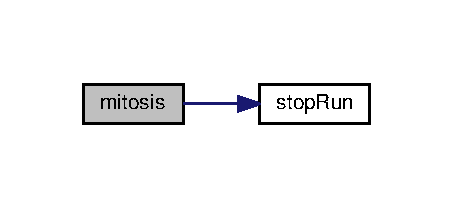
\includegraphics[width=218pt]{cells_8c_a2d9450bd2eebb8f4d645417b92666b87_cgraph}
\end{center}
\end{figure}




Here is the caller graph for this function\-:\nopagebreak
\begin{figure}[H]
\begin{center}
\leavevmode
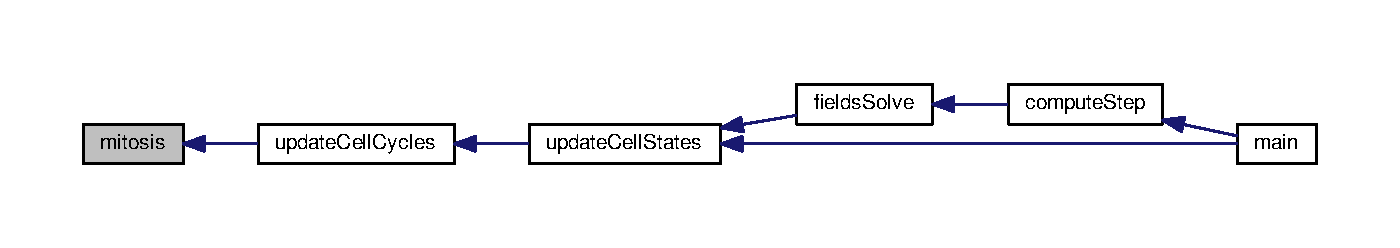
\includegraphics[width=350pt]{cells_8c_a2d9450bd2eebb8f4d645417b92666b87_icgraph}
\end{center}
\end{figure}


\hypertarget{cells_8c_aeeb6dee9938af6fef987f1c949458703}{\index{cells.\-c@{cells.\-c}!update\-Cell\-Counters@{update\-Cell\-Counters}}
\index{update\-Cell\-Counters@{update\-Cell\-Counters}!cells.c@{cells.\-c}}
\subsubsection[{update\-Cell\-Counters}]{\setlength{\rightskip}{0pt plus 5cm}void update\-Cell\-Counters (
\begin{DoxyParamCaption}
{}
\end{DoxyParamCaption}
)}}\label{cells_8c_aeeb6dee9938af6fef987f1c949458703}
This function updates cell counters. 

Definition at line 578 of file cells.\-c.



References globalbc, gnscinst, lnc, localbc, local\-Cell\-Count, nscinst, nscstages, number\-Of\-Counts, tlnc, and total\-Cell\-Count.


\begin{DoxyCode}
579 \{
580   MPI\_Allgather(&\hyperlink{global_8h_a7065c019590815f10169c219f358e7d0}{lnc}, 1, MPI\_INT64\_T, \hyperlink{global_8h_ac3c96b975a3376c555ad22a7d2688b2f}{tlnc}, 1, MPI\_INT64\_T,
581                 MPI\_COMM\_WORLD);
582   MPI\_Allreduce(\hyperlink{global_8h_ab7a46ee61df03f5b6a569427a2f50bec}{localCellCount}, \hyperlink{global_8h_af1a14df9e6c8efece5183d9625039587}{totalCellCount}, 
      \hyperlink{global_8h_a97c5d6b146e57ace62a66400c433aa4d}{numberOfCounts},
583                 MPI\_INT64\_T, MPI\_SUM, MPI\_COMM\_WORLD);
584   MPI\_Allreduce(\hyperlink{global_8h_a1d0cb64baa35f225f63d7e205a36d530}{nscinst}, \hyperlink{global_8h_a386202056f933c1cbadbc5b061909997}{gnscinst}, \hyperlink{global_8h_a612536506e4e3cb48d8e88b795c8beed}{nscstages},
585                 MPI\_INT64\_T, MPI\_SUM, MPI\_COMM\_WORLD);
586   MPI\_Allreduce(&\hyperlink{global_8h_acffece8fb8e971c4a430ae58e28c4980}{localbc}, &\hyperlink{global_8h_ac9f1b6972c68d3ec0bdcf6af318a09e1}{globalbc}, 1,
587                 MPI\_INT64\_T, MPI\_SUM, MPI\_COMM\_WORLD);
588 \}
\end{DoxyCode}


Here is the caller graph for this function\-:\nopagebreak
\begin{figure}[H]
\begin{center}
\leavevmode
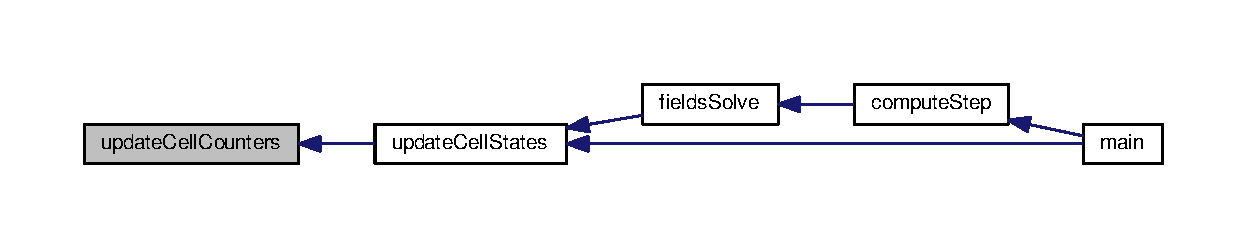
\includegraphics[width=350pt]{cells_8c_aeeb6dee9938af6fef987f1c949458703_icgraph}
\end{center}
\end{figure}


\hypertarget{cells_8c_a718a88fce87f8ebdb87ed2fafed4c5c4}{\index{cells.\-c@{cells.\-c}!update\-Cell\-Cycles@{update\-Cell\-Cycles}}
\index{update\-Cell\-Cycles@{update\-Cell\-Cycles}!cells.c@{cells.\-c}}
\subsubsection[{update\-Cell\-Cycles}]{\setlength{\rightskip}{0pt plus 5cm}int update\-Cell\-Cycles (
\begin{DoxyParamCaption}
{}
\end{DoxyParamCaption}
)}}\label{cells_8c_a718a88fce87f8ebdb87ed2fafed4c5c4}
This function updates cells' cycle phases. 

Definition at line 643 of file cells.\-c.



References celld, cell\-Fields, cells, csize, density\-Critical\-Level1, density\-Critical\-Level2, field\-Critical\-Level1, field\-Critical\-Level2, cell\-Data\-::g1, g1, g2, gf\-Dt, gfields, lg0nc, lg1nc, lg2nc, lmnc, lnc, lnnc, lsnc, m, mitosis(), nc, O\-X\-Y\-G, oxygen, cell\-Data\-::phase, cell\-Data\-::phasetime, rd, rsum, s, sim\-Start, cell\-Data\-::size, and stream.


\begin{DoxyCode}
644 \{
645 
646   \textcolor{keywordtype}{int} c;
647   \textcolor{keywordtype}{double} eps, epsCancer;
648   \textcolor{keywordtype}{int} lncAtThisStep;
649 
650   eps = \hyperlink{global_8h_a8a758046e5cb8b72210f0fc18cb3b7e1}{densityCriticalLevel1};
651   epsCancer = \hyperlink{global_8h_aeddd5065a64a6a39c79e1dab7c0f9edf}{densityCriticalLevel2};
652 
653   lncAtThisStep = \hyperlink{global_8h_a7065c019590815f10169c219f358e7d0}{lnc};
654 
655   \textcolor{keywordflow}{for} (c = 0; c < lncAtThisStep; c++) \{
656 
657     \textcolor{keywordflow}{if} (outsideTheBox(c)) \{
658       \hyperlink{cells_8c_a96a825c021fe648b7fb171bd2c532ffb}{celld}[c] = 1;
659       \hyperlink{global_8h_a087a95bb36c9b36c708a73ce656fd1f1}{rsum}++;
660       \textcolor{keywordflow}{continue};
661     \}
662 
663     \textcolor{keywordflow}{if} (\hyperlink{cells_8c_a96a825c021fe648b7fb171bd2c532ffb}{celld}[c])
664       \textcolor{keywordflow}{continue};
665 
666     \textcolor{keywordflow}{if} (\hyperlink{global_8h_a42a935b4eec9242e09d47fc1c2b6dba3}{simStart}) \{
667 
668       \textcolor{keywordflow}{if} (\hyperlink{global_8h_a3ea537bde8d64e54770a2bd81e3f00be}{cells}[c].phase != 0
669           && ((\hyperlink{global_8h_a3ea537bde8d64e54770a2bd81e3f00be}{cells}[c].tumor == 0 && \hyperlink{global_8h_a3ea537bde8d64e54770a2bd81e3f00be}{cells}[c].density <= eps)
670               || (\hyperlink{global_8h_a3ea537bde8d64e54770a2bd81e3f00be}{cells}[c].tumor == 1 && \hyperlink{global_8h_a3ea537bde8d64e54770a2bd81e3f00be}{cells}[c].density <= epsCancer)))
671         \hyperlink{global_8h_a3ea537bde8d64e54770a2bd81e3f00be}{cells}[c].\hyperlink{structcellData_afe1297f954440c453b59fcb06992dbd5}{phasetime} += \hyperlink{global_8h_aae6a1dda703fb50b7a8b0f4dc01d82c1}{gfDt} / 3600.0;
672 
673       \textcolor{keywordflow}{switch} (\hyperlink{global_8h_a3ea537bde8d64e54770a2bd81e3f00be}{cells}[c].phase) \{
674 
675       \textcolor{keywordflow}{case} 0:           \textcolor{comment}{/* G0 phase */}
676         \textcolor{keywordflow}{if} (\hyperlink{fields_8h_abe4692639a5f11507faff09f2d37efa8}{gfields} && \hyperlink{fields_8h_a67dd60f843bcdd47eb1503456d0da5de}{oxygen}
677             && \hyperlink{global_8h_a25e4317a1b5bb95a8e71e0e8c4e11f2b}{cellFields}[\hyperlink{fields_8h_a5e74e9586fb0eac40835526c74bcb0bc}{OXYG}][c] < \hyperlink{fields_8h_a5534681dc803f20910d872026257fd75}{fieldCriticalLevel2}[
      \hyperlink{fields_8h_a5e74e9586fb0eac40835526c74bcb0bc}{OXYG}]) \{
678           \hyperlink{global_8h_a3ea537bde8d64e54770a2bd81e3f00be}{cells}[c].\hyperlink{structcellData_accf3aec63bc20b3c99ab4881cb07c05b}{phase} = 5;
679           \hyperlink{global_8h_a3ea537bde8d64e54770a2bd81e3f00be}{cells}[c].\hyperlink{structcellData_afe1297f954440c453b59fcb06992dbd5}{phasetime} = 0;
680           \hyperlink{global_8h_a356af225353f2a5512be222c1354bee3}{lg0nc}--;
681           \hyperlink{global_8h_a97370c479716d79f799616103c487d51}{lnnc}++;
682           \textcolor{keywordflow}{break};
683         \}
684         \textcolor{comment}{/* transition to G1 phase */}
685         \textcolor{keywordflow}{if} ((\hyperlink{global_8h_a3ea537bde8d64e54770a2bd81e3f00be}{cells}[c].tumor == 0 && \hyperlink{global_8h_a3ea537bde8d64e54770a2bd81e3f00be}{cells}[c].density <= eps) ||   \textcolor{comment}{/* enough space for healthy
       cell */}
686             (\hyperlink{global_8h_a3ea537bde8d64e54770a2bd81e3f00be}{cells}[c].tumor == 1 && \hyperlink{global_8h_a3ea537bde8d64e54770a2bd81e3f00be}{cells}[c].density <= epsCancer) || \textcolor{comment}{/* enough space for tumor
       cell */}
687             \hyperlink{global_8h_a0845b4b004824f1fe3cd69db1672fa15}{nc} == 1 ||        \textcolor{comment}{/* only single cell in the simulation */}
688             (\hyperlink{fields_8h_abe4692639a5f11507faff09f2d37efa8}{gfields} && \hyperlink{fields_8h_a67dd60f843bcdd47eb1503456d0da5de}{oxygen} && \hyperlink{global_8h_a25e4317a1b5bb95a8e71e0e8c4e11f2b}{cellFields}[OXYG][c] >= 
      \hyperlink{fields_8h_a3d0360f40f207ac596765b891c46b285}{fieldCriticalLevel1}[OXYG])) \{    \textcolor{comment}{/* sufficient level of oxygen */}
689           \hyperlink{global_8h_a3ea537bde8d64e54770a2bd81e3f00be}{cells}[c].\hyperlink{structcellData_accf3aec63bc20b3c99ab4881cb07c05b}{phase} = 1;
690           \hyperlink{global_8h_a356af225353f2a5512be222c1354bee3}{lg0nc}--;
691           \hyperlink{global_8h_a59dc7e07b6be86e29bd0e9f3f18c3ca2}{lg1nc}++;
692           \textcolor{keywordflow}{break};
693         \}
694         \textcolor{keywordflow}{break};
695       \textcolor{keywordflow}{case} 1:           \textcolor{comment}{/* G1 phase */}
696         \textcolor{comment}{/* transition to G0 or Necrotic phase */}
697         \textcolor{keywordflow}{if} ((\hyperlink{global_8h_a3ea537bde8d64e54770a2bd81e3f00be}{cells}[c].tumor == 0 && \hyperlink{global_8h_a3ea537bde8d64e54770a2bd81e3f00be}{cells}[c].density > eps) ||    \textcolor{comment}{/* too crowdy for healthy cell 
      */}
698             (\hyperlink{global_8h_a3ea537bde8d64e54770a2bd81e3f00be}{cells}[c].tumor == 1 && \hyperlink{global_8h_a3ea537bde8d64e54770a2bd81e3f00be}{cells}[c].density > epsCancer) ||  \textcolor{comment}{/* too crowdy for tumor
       cell */}
699             (\hyperlink{fields_8h_abe4692639a5f11507faff09f2d37efa8}{gfields} && \hyperlink{fields_8h_a67dd60f843bcdd47eb1503456d0da5de}{oxygen} && \hyperlink{global_8h_a25e4317a1b5bb95a8e71e0e8c4e11f2b}{cellFields}[OXYG][c] < 
      \hyperlink{fields_8h_a3d0360f40f207ac596765b891c46b285}{fieldCriticalLevel1}[OXYG])) \{    \textcolor{comment}{/* too low oxygen level */}
700           \textcolor{keywordflow}{if} (\hyperlink{fields_8h_abe4692639a5f11507faff09f2d37efa8}{gfields} && \hyperlink{fields_8h_a67dd60f843bcdd47eb1503456d0da5de}{oxygen} && \hyperlink{global_8h_a25e4317a1b5bb95a8e71e0e8c4e11f2b}{cellFields}[OXYG][c] < 
      \hyperlink{fields_8h_a5534681dc803f20910d872026257fd75}{fieldCriticalLevel2}[OXYG]) \{ \textcolor{comment}{/* transition to Necrotic phase */}
701             \hyperlink{global_8h_a3ea537bde8d64e54770a2bd81e3f00be}{cells}[c].\hyperlink{structcellData_accf3aec63bc20b3c99ab4881cb07c05b}{phase} = 5;
702             \hyperlink{global_8h_a3ea537bde8d64e54770a2bd81e3f00be}{cells}[c].\hyperlink{structcellData_afe1297f954440c453b59fcb06992dbd5}{phasetime} = 0;
703             \hyperlink{global_8h_a59dc7e07b6be86e29bd0e9f3f18c3ca2}{lg1nc}--;
704             \hyperlink{global_8h_a97370c479716d79f799616103c487d51}{lnnc}++;
705           \} \textcolor{keywordflow}{else} \{      \textcolor{comment}{/* transition to G0 phase */}
706             \hyperlink{global_8h_a3ea537bde8d64e54770a2bd81e3f00be}{cells}[c].\hyperlink{structcellData_accf3aec63bc20b3c99ab4881cb07c05b}{phase} = 0;
707             \hyperlink{global_8h_a59dc7e07b6be86e29bd0e9f3f18c3ca2}{lg1nc}--;
708             \hyperlink{global_8h_a356af225353f2a5512be222c1354bee3}{lg0nc}++;
709           \}
710           \textcolor{keywordflow}{break};
711         \}
712         \textcolor{comment}{/* cells grow in phase G1 */}
713         \textcolor{keywordflow}{if} (\hyperlink{global_8h_a3ea537bde8d64e54770a2bd81e3f00be}{cells}[c].size < \hyperlink{global_8h_a39fd0cf73801b603ea78d20e05d8cfd3}{csize}) \{
714           \hyperlink{global_8h_a3ea537bde8d64e54770a2bd81e3f00be}{cells}[c].\hyperlink{structcellData_aba3c5d750d5dbd6e86c11ecaca62885e}{size} +=
715             (\hyperlink{global_8h_a39fd0cf73801b603ea78d20e05d8cfd3}{csize} -
716              pow(2.0,
717                  -(1.0 / 3.0)) * \hyperlink{global_8h_a39fd0cf73801b603ea78d20e05d8cfd3}{csize}) * (\hyperlink{global_8h_aae6a1dda703fb50b7a8b0f4dc01d82c1}{gfDt}) / (3600.0 *
718                      \hyperlink{global_8h_a3ea537bde8d64e54770a2bd81e3f00be}{cells}[c].\hyperlink{structcellData_a581debe7d16bce9d187b97855f4e99d4}{g1});
719         \}
720         \textcolor{keywordflow}{if} (\hyperlink{global_8h_a3ea537bde8d64e54770a2bd81e3f00be}{cells}[c].size > \hyperlink{global_8h_a39fd0cf73801b603ea78d20e05d8cfd3}{csize})
721           \hyperlink{global_8h_a3ea537bde8d64e54770a2bd81e3f00be}{cells}[c].\hyperlink{structcellData_aba3c5d750d5dbd6e86c11ecaca62885e}{size} = \hyperlink{global_8h_a39fd0cf73801b603ea78d20e05d8cfd3}{csize};
722         \textcolor{keywordflow}{if} (\hyperlink{global_8h_a3ea537bde8d64e54770a2bd81e3f00be}{cells}[c].phasetime >= \hyperlink{global_8h_a3ea537bde8d64e54770a2bd81e3f00be}{cells}[c].\hyperlink{global_8h_a581debe7d16bce9d187b97855f4e99d4}{g1}) \{
723           \textcolor{keywordtype}{int} death;
724           \hyperlink{global_8h_a3ea537bde8d64e54770a2bd81e3f00be}{cells}[c].\hyperlink{structcellData_accf3aec63bc20b3c99ab4881cb07c05b}{phase} = 2;
725           \hyperlink{global_8h_a3ea537bde8d64e54770a2bd81e3f00be}{cells}[c].\hyperlink{structcellData_afe1297f954440c453b59fcb06992dbd5}{phasetime} = 0;
726           \hyperlink{global_8h_a59dc7e07b6be86e29bd0e9f3f18c3ca2}{lg1nc}--;
727           \hyperlink{global_8h_af5e326c959f5815222d8f8e3f4d66419}{lsnc}++;
728           \textcolor{keywordflow}{if} (\hyperlink{global_8h_a3ea537bde8d64e54770a2bd81e3f00be}{cells}[c].tumor == 0) \{
729             death = (sprng(\hyperlink{global_8h_a5340130b6fb2647cef6b71354e27b0d4}{stream}) < \hyperlink{global_8h_a0d2a1379adf81ce5f962f3c9263e81e9}{rd} ? 1 : 0);
730             \textcolor{keywordflow}{if} (death) \{
731               \hyperlink{cells_8c_a96a825c021fe648b7fb171bd2c532ffb}{celld}[c] = 1;
732               \hyperlink{global_8h_a087a95bb36c9b36c708a73ce656fd1f1}{rsum}++;
733             \}
734           \}
735         \}
736         \textcolor{keywordflow}{break};
737       \textcolor{keywordflow}{case} 2:           \textcolor{comment}{/* S phase */}
738         \textcolor{keywordflow}{if} (\hyperlink{fields_8h_abe4692639a5f11507faff09f2d37efa8}{gfields} && \hyperlink{fields_8h_a67dd60f843bcdd47eb1503456d0da5de}{oxygen}
739             && \hyperlink{global_8h_a25e4317a1b5bb95a8e71e0e8c4e11f2b}{cellFields}[OXYG][c] < \hyperlink{fields_8h_a5534681dc803f20910d872026257fd75}{fieldCriticalLevel2}[OXYG]) \{
740           \hyperlink{global_8h_a3ea537bde8d64e54770a2bd81e3f00be}{cells}[c].\hyperlink{structcellData_accf3aec63bc20b3c99ab4881cb07c05b}{phase} = 5;
741           \hyperlink{global_8h_a3ea537bde8d64e54770a2bd81e3f00be}{cells}[c].\hyperlink{structcellData_afe1297f954440c453b59fcb06992dbd5}{phasetime} = 0;
742           \hyperlink{global_8h_af5e326c959f5815222d8f8e3f4d66419}{lsnc}--;
743           \hyperlink{global_8h_a97370c479716d79f799616103c487d51}{lnnc}++;
744           \textcolor{keywordflow}{break};
745         \}
746         \textcolor{keywordflow}{if} (\hyperlink{global_8h_a3ea537bde8d64e54770a2bd81e3f00be}{cells}[c].phasetime >= \hyperlink{global_8h_a3ea537bde8d64e54770a2bd81e3f00be}{cells}[c].\hyperlink{global_8h_a874f74a4dc1c9a0cd9c6e0d79c298f55}{s}) \{
747           \hyperlink{global_8h_a3ea537bde8d64e54770a2bd81e3f00be}{cells}[c].\hyperlink{structcellData_accf3aec63bc20b3c99ab4881cb07c05b}{phase} = 3;
748           \hyperlink{global_8h_a3ea537bde8d64e54770a2bd81e3f00be}{cells}[c].\hyperlink{structcellData_afe1297f954440c453b59fcb06992dbd5}{phasetime} = 0;
749           \hyperlink{global_8h_af5e326c959f5815222d8f8e3f4d66419}{lsnc}--;
750           \hyperlink{global_8h_a17ca9380dca478aa01c68ce4cc8ca720}{lg2nc}++;
751           \textcolor{keywordflow}{break};
752         \}
753         \textcolor{keywordflow}{break};
754       \textcolor{keywordflow}{case} 3:           \textcolor{comment}{/* G2 phase */}
755         \textcolor{keywordflow}{if} (\hyperlink{fields_8h_abe4692639a5f11507faff09f2d37efa8}{gfields} && \hyperlink{fields_8h_a67dd60f843bcdd47eb1503456d0da5de}{oxygen}
756             && \hyperlink{global_8h_a25e4317a1b5bb95a8e71e0e8c4e11f2b}{cellFields}[OXYG][c] < \hyperlink{fields_8h_a5534681dc803f20910d872026257fd75}{fieldCriticalLevel2}[OXYG]) \{
757           \hyperlink{global_8h_a3ea537bde8d64e54770a2bd81e3f00be}{cells}[c].\hyperlink{structcellData_accf3aec63bc20b3c99ab4881cb07c05b}{phase} = 5;
758           \hyperlink{global_8h_a3ea537bde8d64e54770a2bd81e3f00be}{cells}[c].\hyperlink{structcellData_afe1297f954440c453b59fcb06992dbd5}{phasetime} = 0;
759           \hyperlink{global_8h_a17ca9380dca478aa01c68ce4cc8ca720}{lg2nc}--;
760           \hyperlink{global_8h_a97370c479716d79f799616103c487d51}{lnnc}++;
761           \textcolor{keywordflow}{break};
762         \}
763         \textcolor{keywordflow}{if} (\hyperlink{global_8h_a3ea537bde8d64e54770a2bd81e3f00be}{cells}[c].phasetime >= \hyperlink{global_8h_a3ea537bde8d64e54770a2bd81e3f00be}{cells}[c].\hyperlink{global_8h_aee9971139118d56815564304450c4775}{g2}) \{
764           \textcolor{keywordtype}{int} death;
765           \hyperlink{global_8h_a3ea537bde8d64e54770a2bd81e3f00be}{cells}[c].\hyperlink{structcellData_accf3aec63bc20b3c99ab4881cb07c05b}{phase} = 4;
766           \hyperlink{global_8h_a3ea537bde8d64e54770a2bd81e3f00be}{cells}[c].\hyperlink{structcellData_afe1297f954440c453b59fcb06992dbd5}{phasetime} = 0;
767           \hyperlink{global_8h_a17ca9380dca478aa01c68ce4cc8ca720}{lg2nc}--;
768           \hyperlink{global_8h_a002cff2ccc4cfc5b5f85ac5ea285ef9c}{lmnc}++;
769           \textcolor{keywordflow}{if} (\hyperlink{global_8h_a3ea537bde8d64e54770a2bd81e3f00be}{cells}[c].tumor == 0) \{
770             death = (sprng(\hyperlink{global_8h_a5340130b6fb2647cef6b71354e27b0d4}{stream}) < \hyperlink{global_8h_a0d2a1379adf81ce5f962f3c9263e81e9}{rd} ? 1 : 0);
771             \textcolor{keywordflow}{if} (death) \{
772               \hyperlink{cells_8c_a96a825c021fe648b7fb171bd2c532ffb}{celld}[c] = 1;
773               \hyperlink{global_8h_a087a95bb36c9b36c708a73ce656fd1f1}{rsum}++;
774             \}
775           \}
776           \textcolor{keywordflow}{break};
777         \}
778         \textcolor{keywordflow}{break};
779       \textcolor{keywordflow}{case} 4:           \textcolor{comment}{/* M phase */}
780         \textcolor{keywordflow}{if} (\hyperlink{fields_8h_abe4692639a5f11507faff09f2d37efa8}{gfields} && \hyperlink{fields_8h_a67dd60f843bcdd47eb1503456d0da5de}{oxygen}
781             && \hyperlink{global_8h_a25e4317a1b5bb95a8e71e0e8c4e11f2b}{cellFields}[OXYG][c] < \hyperlink{fields_8h_a5534681dc803f20910d872026257fd75}{fieldCriticalLevel2}[OXYG]) \{
782           \hyperlink{global_8h_a3ea537bde8d64e54770a2bd81e3f00be}{cells}[c].\hyperlink{structcellData_accf3aec63bc20b3c99ab4881cb07c05b}{phase} = 5;
783           \hyperlink{global_8h_a3ea537bde8d64e54770a2bd81e3f00be}{cells}[c].\hyperlink{structcellData_afe1297f954440c453b59fcb06992dbd5}{phasetime} = 0;
784           \hyperlink{global_8h_a002cff2ccc4cfc5b5f85ac5ea285ef9c}{lmnc}--;
785           \hyperlink{global_8h_a97370c479716d79f799616103c487d51}{lnnc}++;
786 
787         \} \textcolor{keywordflow}{else} \textcolor{keywordflow}{if} (\hyperlink{global_8h_a3ea537bde8d64e54770a2bd81e3f00be}{cells}[c].phasetime >= \hyperlink{global_8h_a3ea537bde8d64e54770a2bd81e3f00be}{cells}[c].\hyperlink{global_8h_ac51334f57ef8b81c0629c9421798c344}{m}) \{
788           \hyperlink{cells_8c_a2d9450bd2eebb8f4d645417b92666b87}{mitosis}(c);
789           \hyperlink{global_8h_a3ea537bde8d64e54770a2bd81e3f00be}{cells}[c].\hyperlink{structcellData_accf3aec63bc20b3c99ab4881cb07c05b}{phase} = 1;
790           \hyperlink{global_8h_a3ea537bde8d64e54770a2bd81e3f00be}{cells}[c].\hyperlink{structcellData_afe1297f954440c453b59fcb06992dbd5}{phasetime} = 0;
791           \hyperlink{global_8h_a002cff2ccc4cfc5b5f85ac5ea285ef9c}{lmnc}--;
792           \hyperlink{global_8h_a59dc7e07b6be86e29bd0e9f3f18c3ca2}{lg1nc}++;
793         \}
794         \textcolor{keywordflow}{break};
795       \}             \textcolor{comment}{// switch}
796     \}               \textcolor{comment}{// if}
797   \}             \textcolor{comment}{// for loop}
798 
799   \textcolor{comment}{/* update global number of cells */}
800   MPI\_Allreduce(&\hyperlink{global_8h_a7065c019590815f10169c219f358e7d0}{lnc}, &\hyperlink{global_8h_a0845b4b004824f1fe3cd69db1672fa15}{nc}, 1, MPI\_INT64\_T, MPI\_SUM, MPI\_COMM\_WORLD);
801 
802   \textcolor{keywordflow}{return} 0;
803 \}
\end{DoxyCode}


Here is the call graph for this function\-:\nopagebreak
\begin{figure}[H]
\begin{center}
\leavevmode
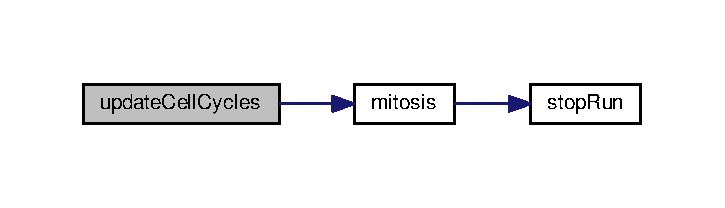
\includegraphics[width=348pt]{cells_8c_a718a88fce87f8ebdb87ed2fafed4c5c4_cgraph}
\end{center}
\end{figure}




Here is the caller graph for this function\-:\nopagebreak
\begin{figure}[H]
\begin{center}
\leavevmode
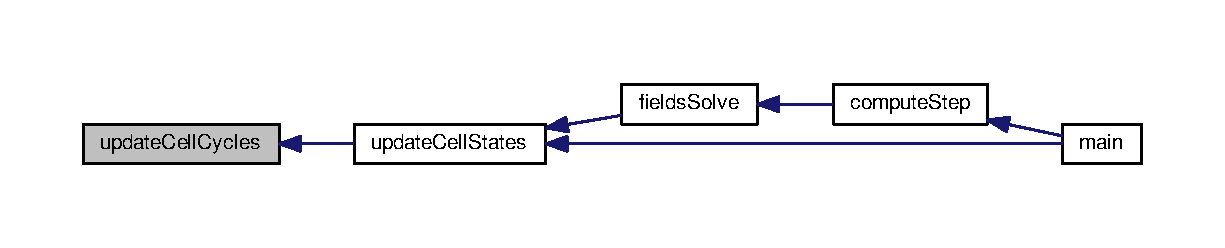
\includegraphics[width=350pt]{cells_8c_a718a88fce87f8ebdb87ed2fafed4c5c4_icgraph}
\end{center}
\end{figure}


\hypertarget{cells_8c_a227256c7da11efa2b4eacedf0a9f37c8}{\index{cells.\-c@{cells.\-c}!update\-Cell\-Positions@{update\-Cell\-Positions}}
\index{update\-Cell\-Positions@{update\-Cell\-Positions}!cells.c@{cells.\-c}}
\subsubsection[{update\-Cell\-Positions}]{\setlength{\rightskip}{0pt plus 5cm}void update\-Cell\-Positions (
\begin{DoxyParamCaption}
{}
\end{DoxyParamCaption}
)}}\label{cells_8c_a227256c7da11efa2b4eacedf0a9f37c8}
This function updates cells' positions. 

Definition at line 603 of file cells.\-c.



References cells, csize, lnc, statistics\-Data\-::mindist, M\-P\-Irank, nc, sim\-Start, statistics, stat\-Out\-Step, step, stream, velocity, cell\-Data\-::x, double\-Vector3d\-::x, cell\-Data\-::y, double\-Vector3d\-::y, cell\-Data\-::z, and double\-Vector3d\-::z.


\begin{DoxyCode}
604 \{
605   \textcolor{keywordtype}{int} c;
606 \textcolor{preprocessor}{#ifdef DEBUG}
607 \textcolor{preprocessor}{}  \textcolor{keywordflow}{if} (\hyperlink{global_8h_a710288ab7d2734acc4566a87a645325d}{MPIrank} == 0 && !(\hyperlink{global_8h_abc16e65f240ed0c8f3e876e8732c0a33}{step} % \hyperlink{global_8h_aab9700fe12cc303ff43e1a35a210128e}{statOutStep})) \{
608     printf(\textcolor{stringliteral}{" Cells movement..."});
609     fflush(stdout);
610   \}
611 \textcolor{preprocessor}{#endif}
612 \textcolor{preprocessor}{}  \textcolor{keywordflow}{if} ((\hyperlink{global_8h_aa28392f90ce59a6b79b9b939fd364a9a}{statistics}.\hyperlink{structstatisticsData_a78455d23ec97258967b76cbb2332b7be}{mindist} >= 0.95 * 2.0 * pow(2.0, -(1.0 / 3.0)) * 
      \hyperlink{global_8h_a39fd0cf73801b603ea78d20e05d8cfd3}{csize}
613        && \hyperlink{global_8h_a42a935b4eec9242e09d47fc1c2b6dba3}{simStart} == 0) || (\hyperlink{global_8h_a0845b4b004824f1fe3cd69db1672fa15}{nc} == 1 && \hyperlink{global_8h_a42a935b4eec9242e09d47fc1c2b6dba3}{simStart} == 0)) \{
614     \hyperlink{global_8h_a42a935b4eec9242e09d47fc1c2b6dba3}{simStart} = 1;
615     \textcolor{keywordflow}{if} (\hyperlink{global_8h_a710288ab7d2734acc4566a87a645325d}{MPIrank} == 0)
616       printf(\textcolor{stringliteral}{"\(\backslash\)nSimulation started.\(\backslash\)n"});
617   \}
618 
619   \textcolor{comment}{/* move cells */}
620   \textcolor{keywordflow}{for} (c = 0; c < \hyperlink{global_8h_a7065c019590815f10169c219f358e7d0}{lnc}; c++) \{
621     \textcolor{keywordflow}{if}(\hyperlink{global_8h_a3ea537bde8d64e54770a2bd81e3f00be}{cells}[c].ctype==1) \textcolor{keywordflow}{continue};
622     \hyperlink{global_8h_a3ea537bde8d64e54770a2bd81e3f00be}{cells}[c].\hyperlink{structcellData_af88b946fb90d5f08b5fb740c70e98c10}{x} += \hyperlink{global_8h_a5ccb3d82df0a6670a0dee2ccd768c0dd}{velocity}[c].\hyperlink{structdoubleVector3d_af88b946fb90d5f08b5fb740c70e98c10}{x} ;
623     \hyperlink{global_8h_a3ea537bde8d64e54770a2bd81e3f00be}{cells}[c].\hyperlink{structcellData_ab927965981178aa1fba979a37168db2a}{y} += \hyperlink{global_8h_a5ccb3d82df0a6670a0dee2ccd768c0dd}{velocity}[c].\hyperlink{structdoubleVector3d_ab927965981178aa1fba979a37168db2a}{y} ;
624     \hyperlink{global_8h_a3ea537bde8d64e54770a2bd81e3f00be}{cells}[c].\hyperlink{structcellData_ab3e6ed577a7c669c19de1f9c1b46c872}{z} += \hyperlink{global_8h_a5ccb3d82df0a6670a0dee2ccd768c0dd}{velocity}[c].\hyperlink{structdoubleVector3d_ab3e6ed577a7c669c19de1f9c1b46c872}{z} ;
625     \textcolor{comment}{/* random movement */}
626     \textcolor{keywordtype}{double} alpha=0.000001;
627     \hyperlink{global_8h_a3ea537bde8d64e54770a2bd81e3f00be}{cells}[c].\hyperlink{structcellData_af88b946fb90d5f08b5fb740c70e98c10}{x} += alpha*(2*sprng(\hyperlink{global_8h_a5340130b6fb2647cef6b71354e27b0d4}{stream})-1);
628     \hyperlink{global_8h_a3ea537bde8d64e54770a2bd81e3f00be}{cells}[c].\hyperlink{structcellData_ab927965981178aa1fba979a37168db2a}{y} += alpha*(2*sprng(\hyperlink{global_8h_a5340130b6fb2647cef6b71354e27b0d4}{stream})-1);
629     \hyperlink{global_8h_a3ea537bde8d64e54770a2bd81e3f00be}{cells}[c].\hyperlink{structcellData_ab3e6ed577a7c669c19de1f9c1b46c872}{z} += alpha*(2*sprng(\hyperlink{global_8h_a5340130b6fb2647cef6b71354e27b0d4}{stream})-1);
630 
631     \textcolor{comment}{// Mark cells that are out of the box and need to be removed}
632     \textcolor{comment}{//if(outside\_the\_box(c)) \{ celld[c]=1; rsum++; \}}
633   \}
634 \textcolor{preprocessor}{#ifdef DEBUG}
635 \textcolor{preprocessor}{}  \textcolor{keywordflow}{if} (\hyperlink{global_8h_a710288ab7d2734acc4566a87a645325d}{MPIrank} == 0 && !(\hyperlink{global_8h_abc16e65f240ed0c8f3e876e8732c0a33}{step} % statOutStep))
636     printf(\textcolor{stringliteral}{"done\(\backslash\)n"});
637 \textcolor{preprocessor}{#endif}
638 \textcolor{preprocessor}{}\}
\end{DoxyCode}


Here is the caller graph for this function\-:\nopagebreak
\begin{figure}[H]
\begin{center}
\leavevmode
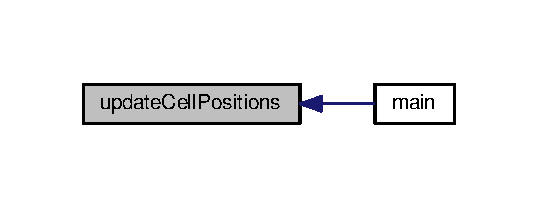
\includegraphics[width=258pt]{cells_8c_a227256c7da11efa2b4eacedf0a9f37c8_icgraph}
\end{center}
\end{figure}


\hypertarget{cells_8c_aeb1f066ef0713a8a50eb1e58784a3d7b}{\index{cells.\-c@{cells.\-c}!update\-Cell\-States@{update\-Cell\-States}}
\index{update\-Cell\-States@{update\-Cell\-States}!cells.c@{cells.\-c}}
\subsubsection[{update\-Cell\-States}]{\setlength{\rightskip}{0pt plus 5cm}void update\-Cell\-States (
\begin{DoxyParamCaption}
{}
\end{DoxyParamCaption}
)}}\label{cells_8c_aeb1f066ef0713a8a50eb1e58784a3d7b}
This function drives the whole cell cycle update. 

Definition at line 825 of file cells.\-c.



References additional\-Scalar\-Field(), cancer, celld, cells\-Death(), lnc, mark\-Middle\-Cancer\-Cell(), nc, nhs, rsum, tgs, update\-Cell\-Counters(), and update\-Cell\-Cycles().


\begin{DoxyCode}
826 \{
827   \textcolor{keywordtype}{int} lnc\_old;
828   \textcolor{comment}{/* number of local cells might change during the update */}
829   lnc\_old = \hyperlink{global_8h_a7065c019590815f10169c219f358e7d0}{lnc};
830   \hyperlink{cells_8c_a96a825c021fe648b7fb171bd2c532ffb}{celld} = (\textcolor{keywordtype}{unsigned} \textcolor{keywordtype}{char} *) calloc(lnc\_old, \textcolor{keyword}{sizeof}(\textcolor{keywordtype}{unsigned} \textcolor{keywordtype}{char}));
831   \hyperlink{global_8h_a087a95bb36c9b36c708a73ce656fd1f1}{rsum} = 0;
832 
833   \hyperlink{cells_8c_a718a88fce87f8ebdb87ed2fafed4c5c4}{updateCellCycles}();
834   \textcolor{keywordflow}{if} (\hyperlink{global_8h_a4c518eee956421a1bf84ad13ab360967}{nhs} > 0 && \hyperlink{global_8h_a0845b4b004824f1fe3cd69db1672fa15}{nc} > \hyperlink{global_8h_a4c518eee956421a1bf84ad13ab360967}{nhs} && \hyperlink{global_8h_ac84ddf735039774c39779789f7afad53}{tgs} == 1 && \hyperlink{global_8h_a543a1902d49aca54ef382bf603a51e27}{cancer} == 0)
835     \hyperlink{cells_8c_a00dbe1f9f23fc7385462c32b89d28cf8}{markMiddleCancerCell}();
836   \textcolor{keywordflow}{if} (\hyperlink{global_8h_a4c518eee956421a1bf84ad13ab360967}{nhs} > 0 && \hyperlink{global_8h_a0845b4b004824f1fe3cd69db1672fa15}{nc} > \hyperlink{global_8h_a4c518eee956421a1bf84ad13ab360967}{nhs})
837     \hyperlink{cells_8c_a8101c456dae07ab9cbd918ccad3a2ff7}{cellsDeath}(lnc\_old);
838   \hyperlink{cells_8c_aeeb6dee9938af6fef987f1c949458703}{updateCellCounters}();
839   \hyperlink{cells_8c_aa2ee543811c23ee4b487102bb71ba9c7}{additionalScalarField}();
840   free(\hyperlink{cells_8c_a96a825c021fe648b7fb171bd2c532ffb}{celld});
841 \}
\end{DoxyCode}


Here is the call graph for this function\-:\nopagebreak
\begin{figure}[H]
\begin{center}
\leavevmode
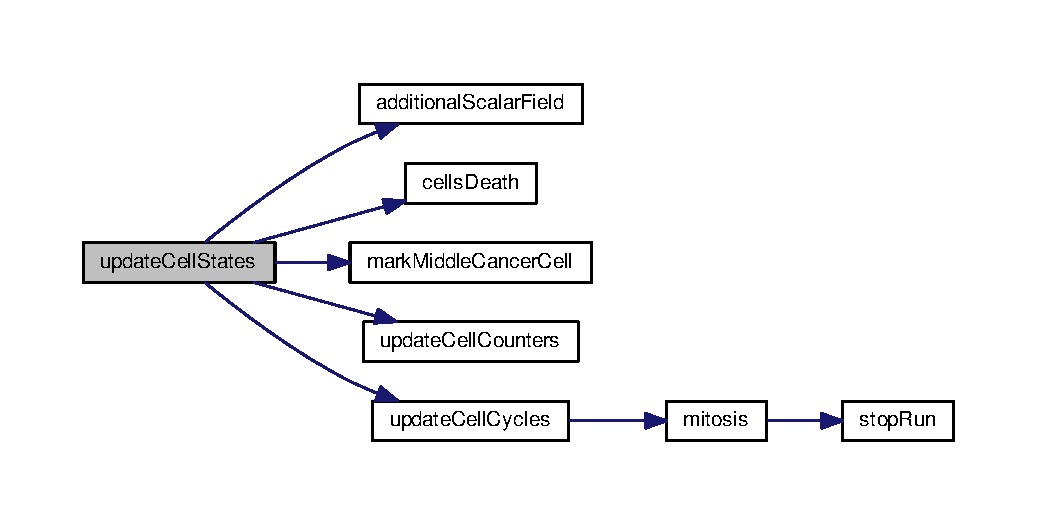
\includegraphics[width=350pt]{cells_8c_aeb1f066ef0713a8a50eb1e58784a3d7b_cgraph}
\end{center}
\end{figure}




Here is the caller graph for this function\-:\nopagebreak
\begin{figure}[H]
\begin{center}
\leavevmode
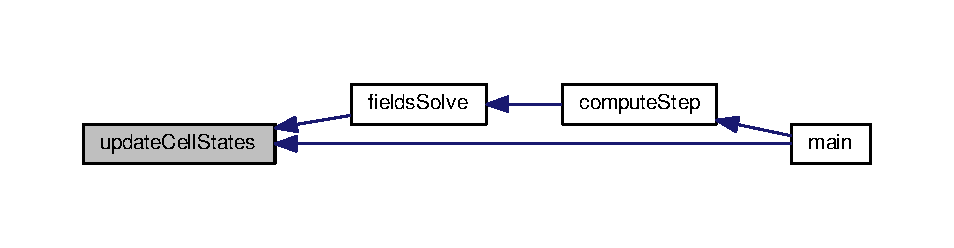
\includegraphics[width=350pt]{cells_8c_aeb1f066ef0713a8a50eb1e58784a3d7b_icgraph}
\end{center}
\end{figure}


\hypertarget{cells_8c_af610aeda76899a9384e98f061c317490}{\index{cells.\-c@{cells.\-c}!update\-Chemotaxis@{update\-Chemotaxis}}
\index{update\-Chemotaxis@{update\-Chemotaxis}!cells.c@{cells.\-c}}
\subsubsection[{update\-Chemotaxis}]{\setlength{\rightskip}{0pt plus 5cm}void update\-Chemotaxis (
\begin{DoxyParamCaption}
{}
\end{DoxyParamCaption}
)}}\label{cells_8c_af610aeda76899a9384e98f061c317490}


Definition at line 590 of file cells.\-c.



References lnc.


\begin{DoxyCode}
591 \{
592   \textcolor{keywordtype}{int} c;
593   \textcolor{keywordflow}{for}(c=0; c<\hyperlink{global_8h_a7065c019590815f10169c219f358e7d0}{lnc}; c++) \{
594 
595 
596   \}
597 \}
\end{DoxyCode}


\subsection{Variable Documentation}
\hypertarget{cells_8c_a96a825c021fe648b7fb171bd2c532ffb}{\index{cells.\-c@{cells.\-c}!celld@{celld}}
\index{celld@{celld}!cells.c@{cells.\-c}}
\subsubsection[{celld}]{\setlength{\rightskip}{0pt plus 5cm}unsigned char$\ast$ celld}}\label{cells_8c_a96a825c021fe648b7fb171bd2c532ffb}


Definition at line 39 of file cells.\-c.


\hypertarget{chemf_8c}{\section{chemf.\-c File Reference}
\label{chemf_8c}\index{chemf.\-c@{chemf.\-c}}
}


contains functions used for solving chemical global fields  


{\ttfamily \#include $<$float.\-h$>$}\\*
{\ttfamily \#include \char`\"{}\-\_\-hypre\-\_\-utilities.\-h\char`\"{}}\\*
{\ttfamily \#include \char`\"{}H\-Y\-P\-R\-E\-\_\-sstruct\-\_\-ls.\-h\char`\"{}}\\*
{\ttfamily \#include \char`\"{}H\-Y\-P\-R\-E\-\_\-parcsr\-\_\-ls.\-h\char`\"{}}\\*
{\ttfamily \#include \char`\"{}H\-Y\-P\-R\-E\-\_\-krylov.\-h\char`\"{}}\\*
{\ttfamily \#include \char`\"{}global.\-h\char`\"{}}\\*
{\ttfamily \#include \char`\"{}fields.\-h\char`\"{}}\\*
Include dependency graph for chemf.\-c\-:\nopagebreak
\begin{figure}[H]
\begin{center}
\leavevmode
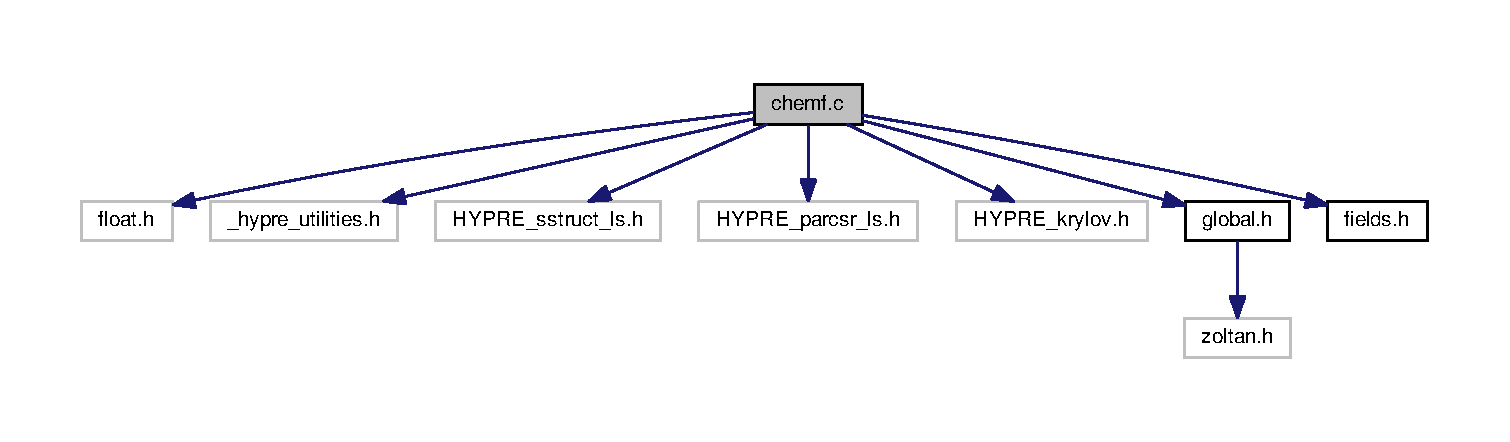
\includegraphics[width=350pt]{chemf_8c__incl}
\end{center}
\end{figure}
\subsection*{Functions}
\begin{DoxyCompactItemize}
\item 
void \hyperlink{chemf_8c_afb692f34ea05262db93f9bf9590b06a7}{chem\-Set\-Boundary} (int coord, int boundary)
\item 
void \hyperlink{chemf_8c_abc9d0a6b17feeff2a62eb6bb38c17ff4}{chem\-Env\-Init\-System} (int nch)
\item 
void \hyperlink{chemf_8c_a5ca738b55b36899ceaa4fe1e6ff38b9f}{chem\-Env\-Cell\-P\-C} (int nch)
\item 
void \hyperlink{chemf_8c_ae67d4d36ecee14805a0b6b0b134b0800}{chem\-Env\-Init\-B\-C} (int nch)
\item 
void \hyperlink{chemf_8c_ad1be1b100191d6ffbd5c3cb0c42549d6}{chem\-Env\-Init\-Solver} (int nch)
\item 
void \hyperlink{chemf_8c_a1f8f7d186d46aafcd792aaf3bee655a7}{chem\-Env\-Solve} (int nch)
\end{DoxyCompactItemize}
\subsection*{Variables}
\begin{DoxyCompactItemize}
\item 
H\-Y\-P\-R\-E\-\_\-\-S\-Struct\-Grid \hyperlink{chemf_8c_ad7a28a5fc279e8b757bdc6a4b57c25be}{chem\-Grid} \mbox{[}\hyperlink{fields_8h_af4afd37668ae33da6377a17adff33029}{N\-C\-H\-E\-M}\mbox{]}
\item 
H\-Y\-P\-R\-E\-\_\-\-S\-Struct\-Graph \hyperlink{chemf_8c_aaac58de32c5dda56ce31654ec3e19337}{chem\-Graph} \mbox{[}\hyperlink{fields_8h_af4afd37668ae33da6377a17adff33029}{N\-C\-H\-E\-M}\mbox{]}
\item 
H\-Y\-P\-R\-E\-\_\-\-S\-Struct\-Stencil \hyperlink{chemf_8c_ae8a36b5c7c6256a7d248a08c71944c73}{chem\-Stencil} \mbox{[}\hyperlink{fields_8h_af4afd37668ae33da6377a17adff33029}{N\-C\-H\-E\-M}\mbox{]}
\item 
H\-Y\-P\-R\-E\-\_\-\-S\-Struct\-Matrix \hyperlink{chemf_8c_ad634e858729e0c04e8b9a4b0a1144b10}{chem\-A} \mbox{[}\hyperlink{fields_8h_af4afd37668ae33da6377a17adff33029}{N\-C\-H\-E\-M}\mbox{]}
\item 
H\-Y\-P\-R\-E\-\_\-\-S\-Struct\-Vector \hyperlink{chemf_8c_afb43e9c9d8160250a03e1b41902473fd}{chemb} \mbox{[}\hyperlink{fields_8h_af4afd37668ae33da6377a17adff33029}{N\-C\-H\-E\-M}\mbox{]}
\item 
H\-Y\-P\-R\-E\-\_\-\-S\-Struct\-Vector \hyperlink{chemf_8c_a48c5bcbe8787c6a6be2a6d5bcdae101f}{chemx} \mbox{[}\hyperlink{fields_8h_af4afd37668ae33da6377a17adff33029}{N\-C\-H\-E\-M}\mbox{]}
\item 
H\-Y\-P\-R\-E\-\_\-\-Par\-C\-S\-R\-Matrix \hyperlink{chemf_8c_a998a7ebb65eb001abcee46c1ea1b1756}{chem\-Par\-A} \mbox{[}\hyperlink{fields_8h_af4afd37668ae33da6377a17adff33029}{N\-C\-H\-E\-M}\mbox{]}
\item 
H\-Y\-P\-R\-E\-\_\-\-Par\-Vector \hyperlink{chemf_8c_af74b7f36ec77fb8e0638db98dd2ee47a}{chem\-Parb} \mbox{[}\hyperlink{fields_8h_af4afd37668ae33da6377a17adff33029}{N\-C\-H\-E\-M}\mbox{]}
\item 
H\-Y\-P\-R\-E\-\_\-\-Par\-Vector \hyperlink{chemf_8c_aae118f98b57f3dda9f036d39db247bb1}{chem\-Parx} \mbox{[}\hyperlink{fields_8h_af4afd37668ae33da6377a17adff33029}{N\-C\-H\-E\-M}\mbox{]}
\item 
H\-Y\-P\-R\-E\-\_\-\-Solver \hyperlink{chemf_8c_a99bbb7b0352d9c850e98287fa45b42c0}{chem\-Solver} \mbox{[}\hyperlink{fields_8h_af4afd37668ae33da6377a17adff33029}{N\-C\-H\-E\-M}\mbox{]}
\item 
H\-Y\-P\-R\-E\-\_\-\-Solver \hyperlink{chemf_8c_a91747632f47bf551e8915e343439777f}{chem\-Precond} \mbox{[}\hyperlink{fields_8h_af4afd37668ae33da6377a17adff33029}{N\-C\-H\-E\-M}\mbox{]}
\item 
int \hyperlink{chemf_8c_a242fb3ba38fb1c6054fd05507394f08b}{chem\-Object\-Type}
\item 
long long \hyperlink{chemf_8c_a14199fec6ea96fe4a4c57bccaff2dfe7}{chem\-Lower} \mbox{[}3\mbox{]}
\item 
long long \hyperlink{chemf_8c_a019f631b2e2795023bf22abef7d9f80e}{chem\-Upper} \mbox{[}3\mbox{]}
\item 
long long \hyperlink{chemf_8c_a397798166a570960b5d468b6df8bf02c}{bc\-Lower} \mbox{[}3\mbox{]}
\item 
long long \hyperlink{chemf_8c_aaea99b8c85fcedb15091dcac991999fd}{bc\-Upper} \mbox{[}3\mbox{]}
\item 
double \hyperlink{chemf_8c_a881c8c944ac83a5c022ee0e236f35e52}{dt} \mbox{[}\hyperlink{fields_8h_af4afd37668ae33da6377a17adff33029}{N\-C\-H\-E\-M}\mbox{]}
\item 
double \hyperlink{chemf_8c_ab35147d777155659aaad43553e3378f4}{chem\-Lambda} = 0.\-25
\item 
char \hyperlink{chemf_8c_a27dc1f70b41e3739d1629663a1d3d0a6}{chfname} \mbox{[}256\mbox{]}
\item 
int \hyperlink{chemf_8c_a26adfe146e722023d7f81bf278bde9e7}{chem\-Iter} \mbox{[}\hyperlink{fields_8h_af4afd37668ae33da6377a17adff33029}{N\-C\-H\-E\-M}\mbox{]}
\item 
double \hyperlink{chemf_8c_ad1178dce1f62833a078c63e911e2e023}{chem\-Z} \mbox{[}\hyperlink{fields_8h_af4afd37668ae33da6377a17adff33029}{N\-C\-H\-E\-M}\mbox{]}
\item 
H\-Y\-P\-R\-E\-\_\-\-S\-Struct\-Variable \hyperlink{chemf_8c_aa73fdbffdd3d43dd503718011b98e41f}{chem\-Vartypes} \mbox{[}1\mbox{]} = \{ H\-Y\-P\-R\-E\-\_\-\-S\-S\-T\-R\-U\-C\-T\-\_\-\-V\-A\-R\-I\-A\-B\-L\-E\-\_\-\-N\-O\-D\-E \}
\item 
int \hyperlink{chemf_8c_a07fef4b421caa5300b13b2ba89422841}{number\-Of\-Iters}
\item 
double $\ast$ \hyperlink{chemf_8c_a614434a804d9a302d1db9603c22b60a7}{chem\-P\-C}
\end{DoxyCompactItemize}


\subsection{Detailed Description}
contains functions used for solving chemical global fields 

Definition in file \hyperlink{chemf_8c_source}{chemf.\-c}.



\subsection{Function Documentation}
\hypertarget{chemf_8c_a5ca738b55b36899ceaa4fe1e6ff38b9f}{\index{chemf.\-c@{chemf.\-c}!chem\-Env\-Cell\-P\-C@{chem\-Env\-Cell\-P\-C}}
\index{chem\-Env\-Cell\-P\-C@{chem\-Env\-Cell\-P\-C}!chemf.c@{chemf.\-c}}
\subsubsection[{chem\-Env\-Cell\-P\-C}]{\setlength{\rightskip}{0pt plus 5cm}void chem\-Env\-Cell\-P\-C (
\begin{DoxyParamCaption}
\item[{int}]{nch}
\end{DoxyParamCaption}
)}}\label{chemf_8c_a5ca738b55b36899ceaa4fe1e6ff38b9f}
This function computes cell production/consumption function based on the interpolated cell density field. 

Definition at line 245 of file chemf.\-c.



References bvsim, chem\-P\-C, dt, field\-Consumption, field\-Production, grid\-Size, N\-G\-L\-O\-B, step, tissue\-Field, vessel\-Field, int64\-Vector3d\-::x, int64\-Vector3d\-::y, and int64\-Vector3d\-::z.


\begin{DoxyCode}
246 \{
247   \textcolor{keywordtype}{int} ch, i, j, k;
248 
249   \textcolor{keywordflow}{if} (\hyperlink{global_8h_abc16e65f240ed0c8f3e876e8732c0a33}{step} == 0)
250     \textcolor{keywordflow}{return};
251 
252   \textcolor{keywordtype}{int} idx = 0;
253   \textcolor{keywordflow}{for} (k = 0; k < \hyperlink{fields_8h_ae67bb9d09bd0919a0ccbc27b387cec72}{gridSize}.\hyperlink{structint64Vector3d_a44624880ae3bb63041297b70cb33408b}{z}; k++)
254     \textcolor{keywordflow}{for} (j = 0; j < \hyperlink{fields_8h_ae67bb9d09bd0919a0ccbc27b387cec72}{gridSize}.\hyperlink{structint64Vector3d_a0cbcba26311a97b8e0763317e105a918}{y}; j++)
255       \textcolor{keywordflow}{for} (i = 0; i < \hyperlink{fields_8h_ae67bb9d09bd0919a0ccbc27b387cec72}{gridSize}.\hyperlink{structint64Vector3d_a040359f45343ce6667f5c66fda5f50e3}{x}; i++, idx++) \{
256         \hyperlink{chemf_8c_a614434a804d9a302d1db9603c22b60a7}{chemPC}[idx] = -\hyperlink{fields_8h_aa36e8f59ad94c5b7629ce29e6d3edc7e}{fieldConsumption}[nch + \hyperlink{fields_8h_aa40ca56600c708a797a77c1db484958d}{NGLOB}] * 
      \hyperlink{fields_8h_a55b7734feef0881a48041f5c8b0fe434}{tissueField}[\hyperlink{fields_8h_ae67bb9d09bd0919a0ccbc27b387cec72}{gridSize}.\hyperlink{structint64Vector3d_a44624880ae3bb63041297b70cb33408b}{z} * \hyperlink{fields_8h_ae67bb9d09bd0919a0ccbc27b387cec72}{gridSize}.\hyperlink{structint64Vector3d_a0cbcba26311a97b8e0763317e105a918}{y} * i + \hyperlink{fields_8h_ae67bb9d09bd0919a0ccbc27b387cec72}{gridSize}.
      \hyperlink{structint64Vector3d_a44624880ae3bb63041297b70cb33408b}{z} * j + k] * \hyperlink{chemf_8c_a881c8c944ac83a5c022ee0e236f35e52}{dt}[nch];
257         \textcolor{keywordflow}{if}(\hyperlink{global_8h_a975a504c34469eed96d609d621cfa35a}{bvsim}) \hyperlink{chemf_8c_a614434a804d9a302d1db9603c22b60a7}{chemPC}[idx]+=\hyperlink{fields_8h_a7bef183ed63be648c7c1f4a63652cb41}{fieldProduction}[nch + 
      \hyperlink{fields_8h_aa40ca56600c708a797a77c1db484958d}{NGLOB}] * \hyperlink{fields_8h_a6ef295c3b0816bc488287d089220ac10}{vesselField}[\hyperlink{fields_8h_ae67bb9d09bd0919a0ccbc27b387cec72}{gridSize}.\hyperlink{structint64Vector3d_a44624880ae3bb63041297b70cb33408b}{z} * \hyperlink{fields_8h_ae67bb9d09bd0919a0ccbc27b387cec72}{gridSize}.\hyperlink{structint64Vector3d_a0cbcba26311a97b8e0763317e105a918}{y} * i + 
      \hyperlink{fields_8h_ae67bb9d09bd0919a0ccbc27b387cec72}{gridSize}.\hyperlink{structint64Vector3d_a44624880ae3bb63041297b70cb33408b}{z} * j +k] * dt[nch] ; \textcolor{comment}{//
      *(cellVolume/boxVolume);//*(1.0/cellVolume);//*dt[nch];//*dt[nch];}
258       \}
259 \}
\end{DoxyCode}


Here is the caller graph for this function\-:\nopagebreak
\begin{figure}[H]
\begin{center}
\leavevmode
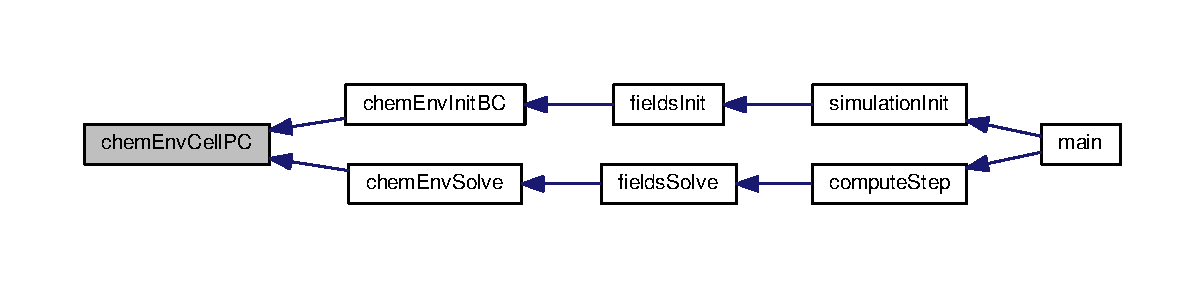
\includegraphics[width=350pt]{chemf_8c_a5ca738b55b36899ceaa4fe1e6ff38b9f_icgraph}
\end{center}
\end{figure}


\hypertarget{chemf_8c_ae67d4d36ecee14805a0b6b0b134b0800}{\index{chemf.\-c@{chemf.\-c}!chem\-Env\-Init\-B\-C@{chem\-Env\-Init\-B\-C}}
\index{chem\-Env\-Init\-B\-C@{chem\-Env\-Init\-B\-C}!chemf.c@{chemf.\-c}}
\subsubsection[{chem\-Env\-Init\-B\-C}]{\setlength{\rightskip}{0pt plus 5cm}void chem\-Env\-Init\-B\-C (
\begin{DoxyParamCaption}
\item[{int}]{nch}
\end{DoxyParamCaption}
)}}\label{chemf_8c_ae67d4d36ecee14805a0b6b0b134b0800}
This function initializes boundary conditions for a given chemical field. 

Definition at line 264 of file chemf.\-c.



References bc\-Lower, bc\-Upper, chem\-A, chemb, chem\-Env\-Cell\-P\-C(), chem\-Grid, chem\-Lower, chem\-Object\-Type, chem\-P\-C, chem\-Set\-Boundary(), chem\-Upper, chemx, chem\-Z, field\-B\-C, field\-I\-C\-Mean, grid\-Size, m, M\-P\-I\-\_\-\-C\-A\-R\-T\-\_\-\-C\-O\-M\-M, M\-P\-Icoords, M\-P\-Idim, M\-P\-Irank, N\-G\-L\-O\-B, int64\-Vector3d\-::x, int64\-Vector3d\-::y, and int64\-Vector3d\-::z.


\begin{DoxyCode}
265 \{
266   \textcolor{keywordtype}{int} i, j, k;
267   \textcolor{keywordtype}{int} \hyperlink{global_8h_ac51334f57ef8b81c0629c9421798c344}{m};
268   \textcolor{keywordtype}{int} nentries = 1;
269   \textcolor{keywordtype}{long} \textcolor{keywordtype}{long} stencil\_indices[1];
270   \textcolor{keywordtype}{long} \textcolor{keywordtype}{long} nvalues = \hyperlink{fields_8h_ae67bb9d09bd0919a0ccbc27b387cec72}{gridSize}.\hyperlink{structint64Vector3d_a040359f45343ce6667f5c66fda5f50e3}{x} * \hyperlink{fields_8h_ae67bb9d09bd0919a0ccbc27b387cec72}{gridSize}.\hyperlink{structint64Vector3d_a0cbcba26311a97b8e0763317e105a918}{y} * \hyperlink{fields_8h_ae67bb9d09bd0919a0ccbc27b387cec72}{gridSize}.
      \hyperlink{structint64Vector3d_a44624880ae3bb63041297b70cb33408b}{z};
271   \textcolor{keywordtype}{double} *values, *bvalues;
272   \textcolor{comment}{/* stdout redirected to file */}
273   \textcolor{comment}{//switchStdOut(chfname);}
274 
275   \hyperlink{chemf_8c_a614434a804d9a302d1db9603c22b60a7}{chemPC} = (\textcolor{keywordtype}{double} *) calloc(nvalues, \textcolor{keyword}{sizeof}(\textcolor{keywordtype}{double}));
276   values = calloc(nvalues, \textcolor{keyword}{sizeof}(\textcolor{keywordtype}{double}));
277   bvalues = calloc(nvalues, \textcolor{keyword}{sizeof}(\textcolor{keywordtype}{double}));
278 
279   \hyperlink{chemf_8c_a5ca738b55b36899ceaa4fe1e6ff38b9f}{chemEnvCellPC}(nch);
280 
281   \textcolor{comment}{/* 5. SETUP STRUCT VECTORS FOR B AND X */}
282 
283   \textcolor{comment}{/* create an empty vector object */}
284   HYPRE\_SStructVectorCreate(\hyperlink{global_8h_a34ac355617a6a906e1f3e7832aeb0073}{MPI\_CART\_COMM}, \hyperlink{chemf_8c_ad7a28a5fc279e8b757bdc6a4b57c25be}{chemGrid}[nch], &
      \hyperlink{chemf_8c_afb43e9c9d8160250a03e1b41902473fd}{chemb}[nch]);
285   HYPRE\_SStructVectorCreate(\hyperlink{global_8h_a34ac355617a6a906e1f3e7832aeb0073}{MPI\_CART\_COMM}, \hyperlink{chemf_8c_ad7a28a5fc279e8b757bdc6a4b57c25be}{chemGrid}[nch], &
      \hyperlink{chemf_8c_a48c5bcbe8787c6a6be2a6d5bcdae101f}{chemx}[nch]);
286 
287   \textcolor{comment}{/* as with the matrix, set the appropriate object type for the vectors */}
288   HYPRE\_SStructVectorSetObjectType(\hyperlink{chemf_8c_afb43e9c9d8160250a03e1b41902473fd}{chemb}[nch], \hyperlink{chemf_8c_a242fb3ba38fb1c6054fd05507394f08b}{chemObjectType});
289   HYPRE\_SStructVectorSetObjectType(\hyperlink{chemf_8c_a48c5bcbe8787c6a6be2a6d5bcdae101f}{chemx}[nch], \hyperlink{chemf_8c_a242fb3ba38fb1c6054fd05507394f08b}{chemObjectType});
290 
291   \textcolor{comment}{/* indicate that the vector coefficients are ready to be set */}
292   HYPRE\_SStructVectorInitialize(\hyperlink{chemf_8c_afb43e9c9d8160250a03e1b41902473fd}{chemb}[nch]);
293   HYPRE\_SStructVectorInitialize(\hyperlink{chemf_8c_a48c5bcbe8787c6a6be2a6d5bcdae101f}{chemx}[nch]);
294 
295   \textcolor{comment}{/* set the values */}
296   m = 0;
297   \textcolor{keywordflow}{for} (k = \hyperlink{chemf_8c_a14199fec6ea96fe4a4c57bccaff2dfe7}{chemLower}[2]; k <= \hyperlink{chemf_8c_a019f631b2e2795023bf22abef7d9f80e}{chemUpper}[2]; k++)
298     \textcolor{keywordflow}{for} (j = \hyperlink{chemf_8c_a14199fec6ea96fe4a4c57bccaff2dfe7}{chemLower}[1]; j <= \hyperlink{chemf_8c_a019f631b2e2795023bf22abef7d9f80e}{chemUpper}[1]; j++)
299       \textcolor{keywordflow}{for} (i = \hyperlink{chemf_8c_a14199fec6ea96fe4a4c57bccaff2dfe7}{chemLower}[0]; i <= \hyperlink{chemf_8c_a019f631b2e2795023bf22abef7d9f80e}{chemUpper}[0]; i++) \{
300         values[\hyperlink{global_8h_ac51334f57ef8b81c0629c9421798c344}{m}] = \hyperlink{fields_8h_ad0fb86debb3e1b138683ff94a2f51f5b}{fieldICMean}[nch + \hyperlink{fields_8h_aa40ca56600c708a797a77c1db484958d}{NGLOB}];
301         m++;
302       \}
303 
304   HYPRE\_SStructVectorSetBoxValues(\hyperlink{chemf_8c_afb43e9c9d8160250a03e1b41902473fd}{chemb}[nch], 0, \hyperlink{chemf_8c_a14199fec6ea96fe4a4c57bccaff2dfe7}{chemLower}, 
      \hyperlink{chemf_8c_a019f631b2e2795023bf22abef7d9f80e}{chemUpper}, 0,
305                                   values);
306 
307   m = 0;
308   \textcolor{keywordflow}{for} (k = \hyperlink{chemf_8c_a14199fec6ea96fe4a4c57bccaff2dfe7}{chemLower}[2]; k <= \hyperlink{chemf_8c_a019f631b2e2795023bf22abef7d9f80e}{chemUpper}[2]; k++)
309     \textcolor{keywordflow}{for} (j = \hyperlink{chemf_8c_a14199fec6ea96fe4a4c57bccaff2dfe7}{chemLower}[1]; j <= \hyperlink{chemf_8c_a019f631b2e2795023bf22abef7d9f80e}{chemUpper}[1]; j++)
310       \textcolor{keywordflow}{for} (i = \hyperlink{chemf_8c_a14199fec6ea96fe4a4c57bccaff2dfe7}{chemLower}[0]; i <= \hyperlink{chemf_8c_a019f631b2e2795023bf22abef7d9f80e}{chemUpper}[0]; i++) \{
311         values[\hyperlink{global_8h_ac51334f57ef8b81c0629c9421798c344}{m}] = \hyperlink{fields_8h_ad0fb86debb3e1b138683ff94a2f51f5b}{fieldICMean}[nch + \hyperlink{fields_8h_aa40ca56600c708a797a77c1db484958d}{NGLOB}];
312         m++;
313       \}
314 
315   HYPRE\_SStructVectorSetBoxValues(\hyperlink{chemf_8c_a48c5bcbe8787c6a6be2a6d5bcdae101f}{chemx}[nch], 0, \hyperlink{chemf_8c_a14199fec6ea96fe4a4c57bccaff2dfe7}{chemLower}, 
      \hyperlink{chemf_8c_a019f631b2e2795023bf22abef7d9f80e}{chemUpper}, 0,
316                                   values);
317 
318   \textcolor{comment}{/* incorporate boundary conditions; Dirichlet on 6 faces */}
319 
320   \textcolor{keywordflow}{for} (i = 0; i < nvalues; i++)
321     values[i] = \hyperlink{chemf_8c_ad1178dce1f62833a078c63e911e2e023}{chemZ}[nch];
322   \textcolor{keywordflow}{for} (i = 0; i < nvalues; i++)
323     bvalues[i] = \hyperlink{chemf_8c_ad1178dce1f62833a078c63e911e2e023}{chemZ}[nch] * \hyperlink{fields_8h_a80c6ee80e0f056adba2430ab0d21e58f}{fieldBC}[nch + \hyperlink{fields_8h_aa40ca56600c708a797a77c1db484958d}{NGLOB}];
324 
325   \textcolor{keywordflow}{if} (\hyperlink{global_8h_a8220294108e39b58632993a50a7dc4ca}{MPIcoords}[\hyperlink{global_8h_a710288ab7d2734acc4566a87a645325d}{MPIrank}][0] == 0) \{
326     nvalues = nentries * \hyperlink{fields_8h_ae67bb9d09bd0919a0ccbc27b387cec72}{gridSize}.\hyperlink{structint64Vector3d_a0cbcba26311a97b8e0763317e105a918}{y} * \hyperlink{fields_8h_ae67bb9d09bd0919a0ccbc27b387cec72}{gridSize}.\hyperlink{structint64Vector3d_a44624880ae3bb63041297b70cb33408b}{z};
327     \hyperlink{chemf_8c_afb692f34ea05262db93f9bf9590b06a7}{chemSetBoundary}(0, -1);
328     stencil\_indices[0] = 1;
329     HYPRE\_SStructMatrixAddToBoxValues(\hyperlink{chemf_8c_ad634e858729e0c04e8b9a4b0a1144b10}{chemA}[nch], 0, \hyperlink{chemf_8c_a397798166a570960b5d468b6df8bf02c}{bcLower}, 
      \hyperlink{chemf_8c_aaea99b8c85fcedb15091dcac991999fd}{bcUpper}, 0,
330                                       nentries, stencil\_indices, values);
331     HYPRE\_SStructVectorAddToBoxValues(\hyperlink{chemf_8c_afb43e9c9d8160250a03e1b41902473fd}{chemb}[nch], 0, \hyperlink{chemf_8c_a397798166a570960b5d468b6df8bf02c}{bcLower}, 
      \hyperlink{chemf_8c_aaea99b8c85fcedb15091dcac991999fd}{bcUpper}, 0,
332                                       bvalues);
333   \}
334   \textcolor{keywordflow}{if} (\hyperlink{global_8h_a8220294108e39b58632993a50a7dc4ca}{MPIcoords}[\hyperlink{global_8h_a710288ab7d2734acc4566a87a645325d}{MPIrank}][0] == \hyperlink{global_8h_a633835398408aaee46fd56809af73e6c}{MPIdim}[0] - 1) \{
335     nvalues = nentries * \hyperlink{fields_8h_ae67bb9d09bd0919a0ccbc27b387cec72}{gridSize}.\hyperlink{structint64Vector3d_a0cbcba26311a97b8e0763317e105a918}{y} * \hyperlink{fields_8h_ae67bb9d09bd0919a0ccbc27b387cec72}{gridSize}.\hyperlink{structint64Vector3d_a44624880ae3bb63041297b70cb33408b}{z};
336     \hyperlink{chemf_8c_afb692f34ea05262db93f9bf9590b06a7}{chemSetBoundary}(0, 1);
337     stencil\_indices[0] = 2;
338     HYPRE\_SStructMatrixAddToBoxValues(\hyperlink{chemf_8c_ad634e858729e0c04e8b9a4b0a1144b10}{chemA}[nch], 0, \hyperlink{chemf_8c_a397798166a570960b5d468b6df8bf02c}{bcLower}, 
      \hyperlink{chemf_8c_aaea99b8c85fcedb15091dcac991999fd}{bcUpper}, 0,
339                                       nentries, stencil\_indices, values);
340     HYPRE\_SStructVectorAddToBoxValues(\hyperlink{chemf_8c_afb43e9c9d8160250a03e1b41902473fd}{chemb}[nch], 0, \hyperlink{chemf_8c_a397798166a570960b5d468b6df8bf02c}{bcLower}, 
      \hyperlink{chemf_8c_aaea99b8c85fcedb15091dcac991999fd}{bcUpper}, 0,
341                                       bvalues);
342   \}
343   \textcolor{keywordflow}{if} (\hyperlink{global_8h_a8220294108e39b58632993a50a7dc4ca}{MPIcoords}[\hyperlink{global_8h_a710288ab7d2734acc4566a87a645325d}{MPIrank}][1] == 0) \{
344     nvalues = nentries * \hyperlink{fields_8h_ae67bb9d09bd0919a0ccbc27b387cec72}{gridSize}.\hyperlink{structint64Vector3d_a040359f45343ce6667f5c66fda5f50e3}{x} * \hyperlink{fields_8h_ae67bb9d09bd0919a0ccbc27b387cec72}{gridSize}.\hyperlink{structint64Vector3d_a44624880ae3bb63041297b70cb33408b}{z};
345     \hyperlink{chemf_8c_afb692f34ea05262db93f9bf9590b06a7}{chemSetBoundary}(1, -1);
346     stencil\_indices[0] = 3;
347     HYPRE\_SStructMatrixAddToBoxValues(\hyperlink{chemf_8c_ad634e858729e0c04e8b9a4b0a1144b10}{chemA}[nch], 0, \hyperlink{chemf_8c_a397798166a570960b5d468b6df8bf02c}{bcLower}, 
      \hyperlink{chemf_8c_aaea99b8c85fcedb15091dcac991999fd}{bcUpper}, 0,
348                                       nentries, stencil\_indices, values);
349     HYPRE\_SStructVectorAddToBoxValues(\hyperlink{chemf_8c_afb43e9c9d8160250a03e1b41902473fd}{chemb}[nch], 0, \hyperlink{chemf_8c_a397798166a570960b5d468b6df8bf02c}{bcLower}, 
      \hyperlink{chemf_8c_aaea99b8c85fcedb15091dcac991999fd}{bcUpper}, 0,
350                                       bvalues);
351   \}
352   \textcolor{keywordflow}{if} (\hyperlink{global_8h_a8220294108e39b58632993a50a7dc4ca}{MPIcoords}[\hyperlink{global_8h_a710288ab7d2734acc4566a87a645325d}{MPIrank}][1] == \hyperlink{global_8h_a633835398408aaee46fd56809af73e6c}{MPIdim}[1] - 1) \{
353     nvalues = nentries * \hyperlink{fields_8h_ae67bb9d09bd0919a0ccbc27b387cec72}{gridSize}.\hyperlink{structint64Vector3d_a040359f45343ce6667f5c66fda5f50e3}{x} * \hyperlink{fields_8h_ae67bb9d09bd0919a0ccbc27b387cec72}{gridSize}.\hyperlink{structint64Vector3d_a44624880ae3bb63041297b70cb33408b}{z};
354     \hyperlink{chemf_8c_afb692f34ea05262db93f9bf9590b06a7}{chemSetBoundary}(1, 1);
355     stencil\_indices[0] = 4;
356     HYPRE\_SStructMatrixAddToBoxValues(\hyperlink{chemf_8c_ad634e858729e0c04e8b9a4b0a1144b10}{chemA}[nch], 0, \hyperlink{chemf_8c_a397798166a570960b5d468b6df8bf02c}{bcLower}, 
      \hyperlink{chemf_8c_aaea99b8c85fcedb15091dcac991999fd}{bcUpper}, 0,
357                                       nentries, stencil\_indices, values);
358     HYPRE\_SStructVectorAddToBoxValues(\hyperlink{chemf_8c_afb43e9c9d8160250a03e1b41902473fd}{chemb}[nch], 0, \hyperlink{chemf_8c_a397798166a570960b5d468b6df8bf02c}{bcLower}, 
      \hyperlink{chemf_8c_aaea99b8c85fcedb15091dcac991999fd}{bcUpper}, 0,
359                                       bvalues);
360   \}
361   \textcolor{keywordflow}{if} (\hyperlink{global_8h_a8220294108e39b58632993a50a7dc4ca}{MPIcoords}[\hyperlink{global_8h_a710288ab7d2734acc4566a87a645325d}{MPIrank}][2] == 0) \{
362     nvalues = nentries * \hyperlink{fields_8h_ae67bb9d09bd0919a0ccbc27b387cec72}{gridSize}.\hyperlink{structint64Vector3d_a040359f45343ce6667f5c66fda5f50e3}{x} * \hyperlink{fields_8h_ae67bb9d09bd0919a0ccbc27b387cec72}{gridSize}.\hyperlink{structint64Vector3d_a0cbcba26311a97b8e0763317e105a918}{y};
363     \hyperlink{chemf_8c_afb692f34ea05262db93f9bf9590b06a7}{chemSetBoundary}(2, -1);
364     stencil\_indices[0] = 5;
365     HYPRE\_SStructMatrixAddToBoxValues(\hyperlink{chemf_8c_ad634e858729e0c04e8b9a4b0a1144b10}{chemA}[nch], 0, \hyperlink{chemf_8c_a397798166a570960b5d468b6df8bf02c}{bcLower}, 
      \hyperlink{chemf_8c_aaea99b8c85fcedb15091dcac991999fd}{bcUpper}, 0,
366                                       nentries, stencil\_indices, values);
367     HYPRE\_SStructVectorAddToBoxValues(\hyperlink{chemf_8c_afb43e9c9d8160250a03e1b41902473fd}{chemb}[nch], 0, \hyperlink{chemf_8c_a397798166a570960b5d468b6df8bf02c}{bcLower}, 
      \hyperlink{chemf_8c_aaea99b8c85fcedb15091dcac991999fd}{bcUpper}, 0,
368                                       bvalues);
369   \}
370   \textcolor{keywordflow}{if} (\hyperlink{global_8h_a8220294108e39b58632993a50a7dc4ca}{MPIcoords}[\hyperlink{global_8h_a710288ab7d2734acc4566a87a645325d}{MPIrank}][2] == \hyperlink{global_8h_a633835398408aaee46fd56809af73e6c}{MPIdim}[2] - 1) \{
371     nvalues = nentries * \hyperlink{fields_8h_ae67bb9d09bd0919a0ccbc27b387cec72}{gridSize}.\hyperlink{structint64Vector3d_a040359f45343ce6667f5c66fda5f50e3}{x} * \hyperlink{fields_8h_ae67bb9d09bd0919a0ccbc27b387cec72}{gridSize}.\hyperlink{structint64Vector3d_a0cbcba26311a97b8e0763317e105a918}{y};
372     \hyperlink{chemf_8c_afb692f34ea05262db93f9bf9590b06a7}{chemSetBoundary}(2, 1);
373     stencil\_indices[0] = 6;
374     HYPRE\_SStructMatrixAddToBoxValues(\hyperlink{chemf_8c_ad634e858729e0c04e8b9a4b0a1144b10}{chemA}[nch], 0, \hyperlink{chemf_8c_a397798166a570960b5d468b6df8bf02c}{bcLower}, 
      \hyperlink{chemf_8c_aaea99b8c85fcedb15091dcac991999fd}{bcUpper}, 0,
375                                       nentries, stencil\_indices, values);
376     HYPRE\_SStructVectorAddToBoxValues(\hyperlink{chemf_8c_afb43e9c9d8160250a03e1b41902473fd}{chemb}[nch], 0, \hyperlink{chemf_8c_a397798166a570960b5d468b6df8bf02c}{bcLower}, 
      \hyperlink{chemf_8c_aaea99b8c85fcedb15091dcac991999fd}{bcUpper}, 0,
377                                       bvalues);
378   \}
379 
380   \textcolor{comment}{/* add production consumption function to the right side */}
381   HYPRE\_SStructVectorAddToBoxValues(\hyperlink{chemf_8c_afb43e9c9d8160250a03e1b41902473fd}{chemb}[nch], 0, \hyperlink{chemf_8c_a14199fec6ea96fe4a4c57bccaff2dfe7}{chemLower}, 
      \hyperlink{chemf_8c_a019f631b2e2795023bf22abef7d9f80e}{chemUpper}, 0,
382                                     \hyperlink{chemf_8c_a614434a804d9a302d1db9603c22b60a7}{chemPC});
383 
384   free(\hyperlink{chemf_8c_a614434a804d9a302d1db9603c22b60a7}{chemPC});
385   free(values);
386   free(bvalues);
387   \textcolor{comment}{/* stdout brought back */}
388   \textcolor{comment}{//revertStdOut();}
389 \}
\end{DoxyCode}


Here is the call graph for this function\-:\nopagebreak
\begin{figure}[H]
\begin{center}
\leavevmode
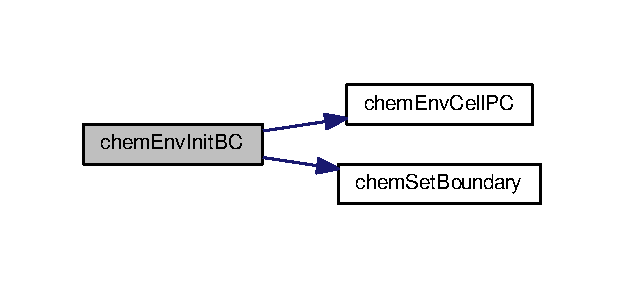
\includegraphics[width=300pt]{chemf_8c_ae67d4d36ecee14805a0b6b0b134b0800_cgraph}
\end{center}
\end{figure}




Here is the caller graph for this function\-:\nopagebreak
\begin{figure}[H]
\begin{center}
\leavevmode
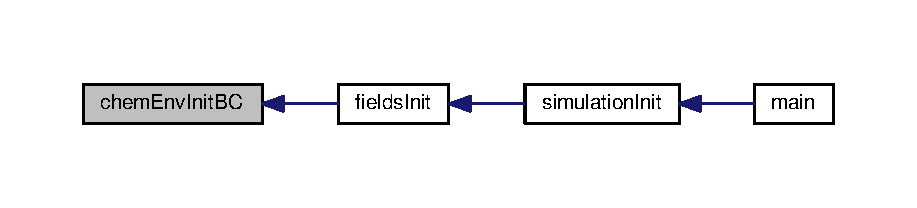
\includegraphics[width=350pt]{chemf_8c_ae67d4d36ecee14805a0b6b0b134b0800_icgraph}
\end{center}
\end{figure}


\hypertarget{chemf_8c_ad1be1b100191d6ffbd5c3cb0c42549d6}{\index{chemf.\-c@{chemf.\-c}!chem\-Env\-Init\-Solver@{chem\-Env\-Init\-Solver}}
\index{chem\-Env\-Init\-Solver@{chem\-Env\-Init\-Solver}!chemf.c@{chemf.\-c}}
\subsubsection[{chem\-Env\-Init\-Solver}]{\setlength{\rightskip}{0pt plus 5cm}void chem\-Env\-Init\-Solver (
\begin{DoxyParamCaption}
\item[{int}]{nch}
\end{DoxyParamCaption}
)}}\label{chemf_8c_ad1be1b100191d6ffbd5c3cb0c42549d6}
This function initializes Hypre for solving a given chemical field. 

Definition at line 394 of file chemf.\-c.



References chem\-A, chemb, chem\-Par\-A, chem\-Parb, chem\-Parx, chem\-Precond, chem\-Solver, chemx, and M\-P\-I\-\_\-\-C\-A\-R\-T\-\_\-\-C\-O\-M\-M.


\begin{DoxyCode}
395 \{
396   \textcolor{comment}{/* stdout redirected to file */}
397   \textcolor{comment}{//switchStdOut(chfname);}
398 
399   HYPRE\_SStructMatrixAssemble(\hyperlink{chemf_8c_ad634e858729e0c04e8b9a4b0a1144b10}{chemA}[nch]);
400   \textcolor{comment}{/* This is a collective call finalizing the vector assembly.}
401 \textcolor{comment}{     The vector is now ``ready to be used'' */}
402   HYPRE\_SStructVectorAssemble(\hyperlink{chemf_8c_afb43e9c9d8160250a03e1b41902473fd}{chemb}[nch]);
403   HYPRE\_SStructVectorAssemble(\hyperlink{chemf_8c_a48c5bcbe8787c6a6be2a6d5bcdae101f}{chemx}[nch]);
404 
405   HYPRE\_SStructMatrixGetObject(\hyperlink{chemf_8c_ad634e858729e0c04e8b9a4b0a1144b10}{chemA}[nch], (\textcolor{keywordtype}{void} **) &\hyperlink{chemf_8c_a998a7ebb65eb001abcee46c1ea1b1756}{chemParA}[nch]);
406   HYPRE\_SStructVectorGetObject(\hyperlink{chemf_8c_afb43e9c9d8160250a03e1b41902473fd}{chemb}[nch], (\textcolor{keywordtype}{void} **) &\hyperlink{chemf_8c_af74b7f36ec77fb8e0638db98dd2ee47a}{chemParb}[nch]);
407   HYPRE\_SStructVectorGetObject(\hyperlink{chemf_8c_a48c5bcbe8787c6a6be2a6d5bcdae101f}{chemx}[nch], (\textcolor{keywordtype}{void} **) &\hyperlink{chemf_8c_aae118f98b57f3dda9f036d39db247bb1}{chemParx}[nch]);
408 
409   HYPRE\_ParCSRPCGCreate(\hyperlink{global_8h_a34ac355617a6a906e1f3e7832aeb0073}{MPI\_CART\_COMM}, &\hyperlink{chemf_8c_a99bbb7b0352d9c850e98287fa45b42c0}{chemSolver}[nch]);
410   HYPRE\_ParCSRPCGSetTol(\hyperlink{chemf_8c_a99bbb7b0352d9c850e98287fa45b42c0}{chemSolver}[nch], 1.0e-12);
411   HYPRE\_ParCSRPCGSetPrintLevel(\hyperlink{chemf_8c_a99bbb7b0352d9c850e98287fa45b42c0}{chemSolver}[nch], 0);
412   HYPRE\_ParCSRPCGSetMaxIter(\hyperlink{chemf_8c_a99bbb7b0352d9c850e98287fa45b42c0}{chemSolver}[nch], 50);
413 
414   HYPRE\_BoomerAMGCreate(&\hyperlink{chemf_8c_a91747632f47bf551e8915e343439777f}{chemPrecond}[nch]);
415   HYPRE\_BoomerAMGSetMaxIter(\hyperlink{chemf_8c_a91747632f47bf551e8915e343439777f}{chemPrecond}[nch], 1);
416   HYPRE\_BoomerAMGSetTol(\hyperlink{chemf_8c_a91747632f47bf551e8915e343439777f}{chemPrecond}[nch], 0.0);
417   HYPRE\_BoomerAMGSetPrintLevel(\hyperlink{chemf_8c_a91747632f47bf551e8915e343439777f}{chemPrecond}[nch], 0);
418   HYPRE\_BoomerAMGSetCoarsenType(\hyperlink{chemf_8c_a91747632f47bf551e8915e343439777f}{chemPrecond}[nch], 6);
419   HYPRE\_BoomerAMGSetRelaxType(\hyperlink{chemf_8c_a91747632f47bf551e8915e343439777f}{chemPrecond}[nch], 6);
420   HYPRE\_BoomerAMGSetNumSweeps(\hyperlink{chemf_8c_a91747632f47bf551e8915e343439777f}{chemPrecond}[nch], 1);
421 
422   HYPRE\_ParCSRPCGSetPrecond(\hyperlink{chemf_8c_a99bbb7b0352d9c850e98287fa45b42c0}{chemSolver}[nch], HYPRE\_BoomerAMGSolve,
423                             HYPRE\_BoomerAMGSetup, \hyperlink{chemf_8c_a91747632f47bf551e8915e343439777f}{chemPrecond}[nch]);
424   HYPRE\_ParCSRPCGSetup(\hyperlink{chemf_8c_a99bbb7b0352d9c850e98287fa45b42c0}{chemSolver}[nch], \hyperlink{chemf_8c_a998a7ebb65eb001abcee46c1ea1b1756}{chemParA}[nch], 
      \hyperlink{chemf_8c_af74b7f36ec77fb8e0638db98dd2ee47a}{chemParb}[nch],
425                        \hyperlink{chemf_8c_aae118f98b57f3dda9f036d39db247bb1}{chemParx}[nch]);
426 
427   \textcolor{comment}{/* stdout brought back */}
428   \textcolor{comment}{//revertStdOut();}
429 \}
\end{DoxyCode}


Here is the caller graph for this function\-:\nopagebreak
\begin{figure}[H]
\begin{center}
\leavevmode
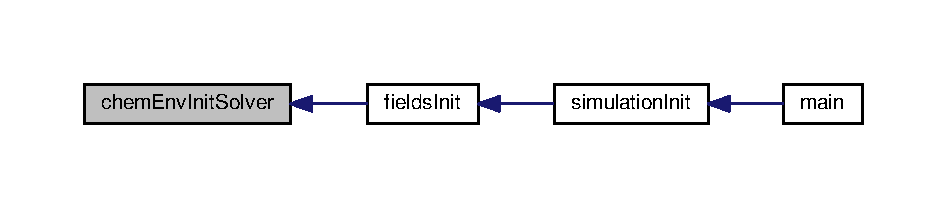
\includegraphics[width=350pt]{chemf_8c_ad1be1b100191d6ffbd5c3cb0c42549d6_icgraph}
\end{center}
\end{figure}


\hypertarget{chemf_8c_abc9d0a6b17feeff2a62eb6bb38c17ff4}{\index{chemf.\-c@{chemf.\-c}!chem\-Env\-Init\-System@{chem\-Env\-Init\-System}}
\index{chem\-Env\-Init\-System@{chem\-Env\-Init\-System}!chemf.c@{chemf.\-c}}
\subsubsection[{chem\-Env\-Init\-System}]{\setlength{\rightskip}{0pt plus 5cm}void chem\-Env\-Init\-System (
\begin{DoxyParamCaption}
\item[{int}]{nch}
\end{DoxyParamCaption}
)}}\label{chemf_8c_abc9d0a6b17feeff2a62eb6bb38c17ff4}
This function initializes grid, stencil and matrix for a given chemical field. 

Definition at line 130 of file chemf.\-c.



References cell\-Fields, chem\-A, chem\-Field, chem\-Graph, chem\-Grid, chem\-Iter, chem\-Lower, chem\-Object\-Type, chem\-Stencil, chem\-Upper, chem\-Vartypes, chem\-Z, csize, csize\-In\-Units, dt, field\-Diff\-Coef, field\-Dt, field\-I\-C\-Mean, field\-Lambda, field\-Max, field\-Min, grid\-End\-Idx, grid\-Resolution, grid\-Size, grid\-Start\-Idx, max\-Cells\-Per\-Proc, M\-P\-I\-\_\-\-C\-A\-R\-T\-\_\-\-C\-O\-M\-M, M\-P\-Irank, N\-G\-L\-O\-B, number\-Of\-Iters, int64\-Vector3d\-::x, int64\-Vector3d\-::y, and int64\-Vector3d\-::z.


\begin{DoxyCode}
131 \{
132   \textcolor{keywordtype}{int} i, j, k, c;
133   \textcolor{keywordtype}{int} entry;
134   \textcolor{keywordtype}{long} \textcolor{keywordtype}{long} offsets[7][3] = \{
135     \{0, 0, 0\}, \{-1, 0, 0\}, \{1, 0, 0\}, \{0, -1, 0\}, \{0, 1, 0\}, \{
136       0, 0,
137       -1
138     \}, \{
139       0,
140       0,
141       1
142     \}
143   \};
144   \textcolor{keywordtype}{double} gridResolutionInUnits; \textcolor{comment}{/* grid resolution in centimeters */}
145 
146   \hyperlink{chemf_8c_a881c8c944ac83a5c022ee0e236f35e52}{dt}[nch] = \hyperlink{fields_8h_ae21d99cc23aefdfc02fbe62cd28784fb}{fieldDt}[nch + \hyperlink{fields_8h_aa40ca56600c708a797a77c1db484958d}{NGLOB}];
147   \hyperlink{chemf_8c_a07fef4b421caa5300b13b2ba89422841}{numberOfIters} = 1;
148   \hyperlink{chemf_8c_a26adfe146e722023d7f81bf278bde9e7}{chemIter}[nch] = 0;
149 
150 \textcolor{comment}{//  sprintf(chfname, "%s/chemSolver.log", logdir);}
151   \textcolor{comment}{/* stdout will go to the file */}
152 \textcolor{comment}{//  switchStdOut(chfname);}
153 
154   \textcolor{comment}{/* 1. INIT GRID */}
155 
156   \textcolor{comment}{/* create an empty 3D grid object */}
157   HYPRE\_SStructGridCreate(\hyperlink{global_8h_a34ac355617a6a906e1f3e7832aeb0073}{MPI\_CART\_COMM}, 3, 1, &\hyperlink{chemf_8c_ad7a28a5fc279e8b757bdc6a4b57c25be}{chemGrid}[nch]);
158 
159   \textcolor{comment}{/* set this process box */}
160   \hyperlink{chemf_8c_a14199fec6ea96fe4a4c57bccaff2dfe7}{chemLower}[0] = \hyperlink{fields_8h_a9154f33f7786c05c61f4d519da14d501}{gridStartIdx}[\hyperlink{global_8h_a710288ab7d2734acc4566a87a645325d}{MPIrank}].\hyperlink{structint64Vector3d_a040359f45343ce6667f5c66fda5f50e3}{x};
161   \hyperlink{chemf_8c_a14199fec6ea96fe4a4c57bccaff2dfe7}{chemLower}[1] = \hyperlink{fields_8h_a9154f33f7786c05c61f4d519da14d501}{gridStartIdx}[\hyperlink{global_8h_a710288ab7d2734acc4566a87a645325d}{MPIrank}].\hyperlink{structint64Vector3d_a0cbcba26311a97b8e0763317e105a918}{y};
162   \hyperlink{chemf_8c_a14199fec6ea96fe4a4c57bccaff2dfe7}{chemLower}[2] = \hyperlink{fields_8h_a9154f33f7786c05c61f4d519da14d501}{gridStartIdx}[\hyperlink{global_8h_a710288ab7d2734acc4566a87a645325d}{MPIrank}].\hyperlink{structint64Vector3d_a44624880ae3bb63041297b70cb33408b}{z};
163 
164   \hyperlink{chemf_8c_a019f631b2e2795023bf22abef7d9f80e}{chemUpper}[0] = \hyperlink{fields_8h_a1d13a1c43b1a6eb6ca088b79ee681b48}{gridEndIdx}[\hyperlink{global_8h_a710288ab7d2734acc4566a87a645325d}{MPIrank}].\hyperlink{structint64Vector3d_a040359f45343ce6667f5c66fda5f50e3}{x};
165   \hyperlink{chemf_8c_a019f631b2e2795023bf22abef7d9f80e}{chemUpper}[1] = \hyperlink{fields_8h_a1d13a1c43b1a6eb6ca088b79ee681b48}{gridEndIdx}[\hyperlink{global_8h_a710288ab7d2734acc4566a87a645325d}{MPIrank}].\hyperlink{structint64Vector3d_a0cbcba26311a97b8e0763317e105a918}{y};
166   \hyperlink{chemf_8c_a019f631b2e2795023bf22abef7d9f80e}{chemUpper}[2] = \hyperlink{fields_8h_a1d13a1c43b1a6eb6ca088b79ee681b48}{gridEndIdx}[\hyperlink{global_8h_a710288ab7d2734acc4566a87a645325d}{MPIrank}].\hyperlink{structint64Vector3d_a44624880ae3bb63041297b70cb33408b}{z};
167 
168   \textcolor{comment}{/* add a new box to the grid */}
169   HYPRE\_SStructGridSetExtents(\hyperlink{chemf_8c_ad7a28a5fc279e8b757bdc6a4b57c25be}{chemGrid}[nch], 0, \hyperlink{chemf_8c_a14199fec6ea96fe4a4c57bccaff2dfe7}{chemLower}, 
      \hyperlink{chemf_8c_a019f631b2e2795023bf22abef7d9f80e}{chemUpper});
170 
171   HYPRE\_SStructGridSetVariables(\hyperlink{chemf_8c_ad7a28a5fc279e8b757bdc6a4b57c25be}{chemGrid}[nch], 0, 1, \hyperlink{chemf_8c_aa73fdbffdd3d43dd503718011b98e41f}{chemVartypes});
172   HYPRE\_SStructGridAssemble(\hyperlink{chemf_8c_ad7a28a5fc279e8b757bdc6a4b57c25be}{chemGrid}[nch]);
173 
174   \textcolor{comment}{//  2. INIT STENCIL}
175   HYPRE\_SStructStencilCreate(3, 7, &\hyperlink{chemf_8c_ae8a36b5c7c6256a7d248a08c71944c73}{chemStencil}[nch]);
176   \textcolor{keywordflow}{for} (entry = 0; entry < 7; entry++)
177     HYPRE\_SStructStencilSetEntry(\hyperlink{chemf_8c_ae8a36b5c7c6256a7d248a08c71944c73}{chemStencil}[nch], entry, offsets[entry],
178                                  0);
179 
180   \textcolor{comment}{// 3. SET UP THE GRAPH}
181   \hyperlink{chemf_8c_a242fb3ba38fb1c6054fd05507394f08b}{chemObjectType} = HYPRE\_PARCSR;
182   HYPRE\_SStructGraphCreate(\hyperlink{global_8h_a34ac355617a6a906e1f3e7832aeb0073}{MPI\_CART\_COMM}, \hyperlink{chemf_8c_ad7a28a5fc279e8b757bdc6a4b57c25be}{chemGrid}[nch], &
      \hyperlink{chemf_8c_aaac58de32c5dda56ce31654ec3e19337}{chemGraph}[nch]);
183   HYPRE\_SStructGraphSetObjectType(\hyperlink{chemf_8c_aaac58de32c5dda56ce31654ec3e19337}{chemGraph}[nch], \hyperlink{chemf_8c_a242fb3ba38fb1c6054fd05507394f08b}{chemObjectType});
184   HYPRE\_SStructGraphSetStencil(\hyperlink{chemf_8c_aaac58de32c5dda56ce31654ec3e19337}{chemGraph}[nch], 0, 0, \hyperlink{chemf_8c_ae8a36b5c7c6256a7d248a08c71944c73}{chemStencil}[nch]);
185   HYPRE\_SStructGraphAssemble(\hyperlink{chemf_8c_aaac58de32c5dda56ce31654ec3e19337}{chemGraph}[nch]);
186 
187   \textcolor{comment}{// 4. SET UP MATRIX}
188   \textcolor{keywordtype}{long} \textcolor{keywordtype}{long} nentries = 7;
189   \textcolor{keywordtype}{long} \textcolor{keywordtype}{long} nvalues;
190   \textcolor{keywordtype}{double} *values;
191   \textcolor{keywordtype}{long} \textcolor{keywordtype}{long} stencil\_indices[7];
192 
193   nvalues = nentries * \hyperlink{fields_8h_ae67bb9d09bd0919a0ccbc27b387cec72}{gridSize}.\hyperlink{structint64Vector3d_a040359f45343ce6667f5c66fda5f50e3}{x} * \hyperlink{fields_8h_ae67bb9d09bd0919a0ccbc27b387cec72}{gridSize}.\hyperlink{structint64Vector3d_a0cbcba26311a97b8e0763317e105a918}{y} * \hyperlink{fields_8h_ae67bb9d09bd0919a0ccbc27b387cec72}{gridSize}.
      \hyperlink{structint64Vector3d_a44624880ae3bb63041297b70cb33408b}{z};
194   \textcolor{comment}{// create an empty matrix object}
195   HYPRE\_SStructMatrixCreate(\hyperlink{global_8h_a34ac355617a6a906e1f3e7832aeb0073}{MPI\_CART\_COMM}, \hyperlink{chemf_8c_aaac58de32c5dda56ce31654ec3e19337}{chemGraph}[nch], &
      \hyperlink{chemf_8c_ad634e858729e0c04e8b9a4b0a1144b10}{chemA}[nch]);
196   HYPRE\_SStructMatrixSetObjectType(\hyperlink{chemf_8c_ad634e858729e0c04e8b9a4b0a1144b10}{chemA}[nch], \hyperlink{chemf_8c_a242fb3ba38fb1c6054fd05507394f08b}{chemObjectType});
197   \textcolor{comment}{// indicate that the matrix coefficients are ready to be set}
198   HYPRE\_SStructMatrixInitialize(\hyperlink{chemf_8c_ad634e858729e0c04e8b9a4b0a1144b10}{chemA}[nch]);
199 
200   values = calloc(nvalues, \textcolor{keyword}{sizeof}(\textcolor{keywordtype}{double}));
201 
202   \textcolor{keywordflow}{for} (j = 0; j < nentries; j++)
203     stencil\_indices[j] = j;
204 
205   gridResolutionInUnits = (\hyperlink{fields_8h_a1c1b24172891a639f9cad84edebeaee9}{gridResolution} / \hyperlink{global_8h_a39fd0cf73801b603ea78d20e05d8cfd3}{csize}) * 
      \hyperlink{global_8h_a5618d8682d7245e8770f85fbf8c2fda5}{csizeInUnits} * 0.0001;
206 
207   \hyperlink{chemf_8c_ad1178dce1f62833a078c63e911e2e023}{chemZ}[nch] =
208     \hyperlink{fields_8h_ad4870e0beb9744bd643b6501c4505d81}{fieldDiffCoef}[nch +
209                   \hyperlink{fields_8h_aa40ca56600c708a797a77c1db484958d}{NGLOB}] * \hyperlink{chemf_8c_a881c8c944ac83a5c022ee0e236f35e52}{dt}[nch] / (gridResolutionInUnits *
210                                       gridResolutionInUnits);
211 
212   \textcolor{comment}{// set the standard stencil at each grid point,}
213   \textcolor{comment}{//  we will fix the boundaries later}
214   \textcolor{keywordflow}{for} (i = 0; i < nvalues; i += nentries) \{
215     values[i] = 1 + 6.0 * \hyperlink{chemf_8c_ad1178dce1f62833a078c63e911e2e023}{chemZ}[nch] + \hyperlink{fields_8h_a2fe4102c6ceed6e01ff5b2f47eb0828d}{fieldLambda}[nch + \hyperlink{fields_8h_aa40ca56600c708a797a77c1db484958d}{NGLOB}] * 
      \hyperlink{chemf_8c_a881c8c944ac83a5c022ee0e236f35e52}{dt}[nch];
216     \textcolor{keywordflow}{for} (j = 1; j < nentries; j++)
217       values[i + j] = -\hyperlink{chemf_8c_ad1178dce1f62833a078c63e911e2e023}{chemZ}[nch];
218   \}
219 
220   HYPRE\_SStructMatrixSetBoxValues(\hyperlink{chemf_8c_ad634e858729e0c04e8b9a4b0a1144b10}{chemA}[nch], 0, \hyperlink{chemf_8c_a14199fec6ea96fe4a4c57bccaff2dfe7}{chemLower}, 
      \hyperlink{chemf_8c_a019f631b2e2795023bf22abef7d9f80e}{chemUpper}, 0,
221                                   nentries, stencil\_indices, values);
222 
223   \textcolor{keywordflow}{for} (k = 0; k < \hyperlink{fields_8h_ae67bb9d09bd0919a0ccbc27b387cec72}{gridSize}.\hyperlink{structint64Vector3d_a44624880ae3bb63041297b70cb33408b}{z}; k++)
224     \textcolor{keywordflow}{for} (j = 0; j < \hyperlink{fields_8h_ae67bb9d09bd0919a0ccbc27b387cec72}{gridSize}.\hyperlink{structint64Vector3d_a0cbcba26311a97b8e0763317e105a918}{y}; j++)
225       \textcolor{keywordflow}{for} (i = 0; i < \hyperlink{fields_8h_ae67bb9d09bd0919a0ccbc27b387cec72}{gridSize}.\hyperlink{structint64Vector3d_a040359f45343ce6667f5c66fda5f50e3}{x}; i++) \{
226         \hyperlink{fields_8h_adb9b18c97bd0384bf977ee57e604626a}{chemField}[nch][\hyperlink{fields_8h_ae67bb9d09bd0919a0ccbc27b387cec72}{gridSize}.\hyperlink{structint64Vector3d_a0cbcba26311a97b8e0763317e105a918}{y} * \hyperlink{fields_8h_ae67bb9d09bd0919a0ccbc27b387cec72}{gridSize}.\hyperlink{structint64Vector3d_a44624880ae3bb63041297b70cb33408b}{z} * i + 
      \hyperlink{fields_8h_ae67bb9d09bd0919a0ccbc27b387cec72}{gridSize}.\hyperlink{structint64Vector3d_a44624880ae3bb63041297b70cb33408b}{z} * j + k] =
227           \hyperlink{fields_8h_ad0fb86debb3e1b138683ff94a2f51f5b}{fieldICMean}[nch + \hyperlink{fields_8h_aa40ca56600c708a797a77c1db484958d}{NGLOB}];
228       \}
229   \hyperlink{fields_8h_afa26584ead914a9e160c467308ed156a}{fieldMax}[nch + \hyperlink{fields_8h_aa40ca56600c708a797a77c1db484958d}{NGLOB}] = \hyperlink{fields_8h_ad0fb86debb3e1b138683ff94a2f51f5b}{fieldICMean}[nch + \hyperlink{fields_8h_aa40ca56600c708a797a77c1db484958d}{NGLOB}];
230   \hyperlink{fields_8h_adc4b9b908fa47243451f8725e6210e34}{fieldMin}[nch + \hyperlink{fields_8h_aa40ca56600c708a797a77c1db484958d}{NGLOB}] = \hyperlink{fields_8h_ad0fb86debb3e1b138683ff94a2f51f5b}{fieldICMean}[nch + \hyperlink{fields_8h_aa40ca56600c708a797a77c1db484958d}{NGLOB}];
231 
232   \textcolor{keywordflow}{for} (c = 0; c < \hyperlink{global_8h_a2de426dd266cfdaaf6fb52ba3dc2740a}{maxCellsPerProc}; c++) \{
233     \hyperlink{global_8h_a25e4317a1b5bb95a8e71e0e8c4e11f2b}{cellFields}[nch + \hyperlink{fields_8h_aa40ca56600c708a797a77c1db484958d}{NGLOB}][c] = \hyperlink{fields_8h_ad0fb86debb3e1b138683ff94a2f51f5b}{fieldICMean}[nch + 
      \hyperlink{fields_8h_aa40ca56600c708a797a77c1db484958d}{NGLOB}];
234   \}
235 
236   free(values);
237   \textcolor{comment}{/* stdout brought back */}
238 \textcolor{comment}{//  revertStdOut();}
239 \}
\end{DoxyCode}


Here is the caller graph for this function\-:\nopagebreak
\begin{figure}[H]
\begin{center}
\leavevmode
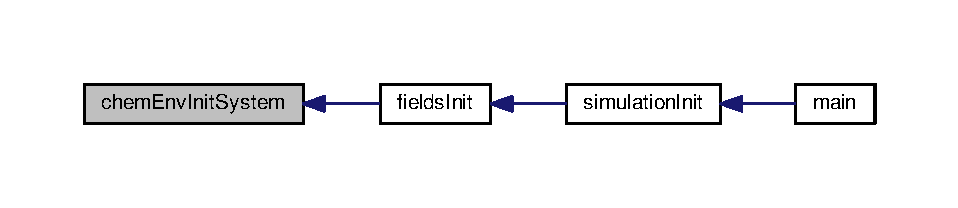
\includegraphics[width=350pt]{chemf_8c_abc9d0a6b17feeff2a62eb6bb38c17ff4_icgraph}
\end{center}
\end{figure}


\hypertarget{chemf_8c_a1f8f7d186d46aafcd792aaf3bee655a7}{\index{chemf.\-c@{chemf.\-c}!chem\-Env\-Solve@{chem\-Env\-Solve}}
\index{chem\-Env\-Solve@{chem\-Env\-Solve}!chemf.c@{chemf.\-c}}
\subsubsection[{chem\-Env\-Solve}]{\setlength{\rightskip}{0pt plus 5cm}void chem\-Env\-Solve (
\begin{DoxyParamCaption}
\item[{int}]{nch}
\end{DoxyParamCaption}
)}}\label{chemf_8c_a1f8f7d186d46aafcd792aaf3bee655a7}
This is a driving function for solving next time step of a given chemical field. 

Definition at line 435 of file chemf.\-c.



References bc\-Lower, bc\-Upper, chemb, chem\-Env\-Cell\-P\-C(), chem\-Field, chem\-Iter, chem\-Lower, chem\-Par\-A, chem\-Parb, chem\-Parx, chem\-P\-C, chem\-Set\-Boundary(), chem\-Solver, chem\-Upper, chemx, chem\-Z, field\-B\-C, field\-Max, field\-Min, field\-Name, gf\-Iter, gf\-Iter\-Per\-Step, grid\-Size, M\-P\-Icoords, M\-P\-Idim, M\-P\-Irank, N\-G\-L\-O\-B, number\-Of\-Iters, stat\-Out\-Step, step, int64\-Vector3d\-::x, int64\-Vector3d\-::y, and int64\-Vector3d\-::z.


\begin{DoxyCode}
436 \{
437   \textcolor{keywordtype}{int} i, j, k;
438   \textcolor{keywordtype}{int} idx;
439   \textcolor{keywordtype}{double} *values;
440   \textcolor{keywordtype}{int} stepIter = 0;
441   \textcolor{keywordtype}{long} \textcolor{keywordtype}{long} nvalues = \hyperlink{fields_8h_ae67bb9d09bd0919a0ccbc27b387cec72}{gridSize}.\hyperlink{structint64Vector3d_a040359f45343ce6667f5c66fda5f50e3}{x} * \hyperlink{fields_8h_ae67bb9d09bd0919a0ccbc27b387cec72}{gridSize}.\hyperlink{structint64Vector3d_a0cbcba26311a97b8e0763317e105a918}{y} * \hyperlink{fields_8h_ae67bb9d09bd0919a0ccbc27b387cec72}{gridSize}.
      \hyperlink{structint64Vector3d_a44624880ae3bb63041297b70cb33408b}{z};
442 \textcolor{preprocessor}{#ifdef DEBUG}
443 \textcolor{preprocessor}{}  \textcolor{keywordflow}{if} (\hyperlink{global_8h_a710288ab7d2734acc4566a87a645325d}{MPIrank} == 0 && !(\hyperlink{global_8h_abc16e65f240ed0c8f3e876e8732c0a33}{step} % \hyperlink{global_8h_aab9700fe12cc303ff43e1a35a210128e}{statOutStep}) && \hyperlink{global_8h_ab2e483b60cc15741bd6281688f31edbc}{gfIter} == 0) \{
444     printf(\textcolor{stringliteral}{" Solving field: %s..."}, \hyperlink{fields_8h_a1a12b04329495ce82cf21a9d42b71f1c}{fieldName}[nch + \hyperlink{fields_8h_aa40ca56600c708a797a77c1db484958d}{NGLOB}]);
445     fflush(stdout);
446   \}
447 \textcolor{preprocessor}{#endif}
448 \textcolor{preprocessor}{}  \textcolor{comment}{/* redirecting stdout to log file */}
449   \textcolor{comment}{//switchStdOut(chfname);}
450 
451   values = (\textcolor{keywordtype}{double} *) calloc(nvalues, \textcolor{keyword}{sizeof}(\textcolor{keywordtype}{double}));
452   \hyperlink{chemf_8c_a614434a804d9a302d1db9603c22b60a7}{chemPC} = (\textcolor{keywordtype}{double} *) calloc(nvalues, \textcolor{keyword}{sizeof}(\textcolor{keywordtype}{double}));
453   \hyperlink{chemf_8c_a5ca738b55b36899ceaa4fe1e6ff38b9f}{chemEnvCellPC}(nch);
454 
455   \hyperlink{fields_8h_adc4b9b908fa47243451f8725e6210e34}{fieldMin}[nch + \hyperlink{fields_8h_aa40ca56600c708a797a77c1db484958d}{NGLOB}] = DBL\_MAX;
456   \hyperlink{fields_8h_afa26584ead914a9e160c467308ed156a}{fieldMax}[nch + \hyperlink{fields_8h_aa40ca56600c708a797a77c1db484958d}{NGLOB}] = DBL\_MIN;
457 
458   \textcolor{keywordflow}{while} (stepIter < \hyperlink{chemf_8c_a07fef4b421caa5300b13b2ba89422841}{numberOfIters}) \{
459     \textcolor{keywordflow}{if} (\hyperlink{chemf_8c_a26adfe146e722023d7f81bf278bde9e7}{chemIter}[nch] > 0) \{
460       \textcolor{comment}{/* update right hand side */}
461       HYPRE\_SStructVectorGetBoxValues(\hyperlink{chemf_8c_a48c5bcbe8787c6a6be2a6d5bcdae101f}{chemx}[nch], 0, \hyperlink{chemf_8c_a14199fec6ea96fe4a4c57bccaff2dfe7}{chemLower}, 
      \hyperlink{chemf_8c_a019f631b2e2795023bf22abef7d9f80e}{chemUpper},
462                                       0, values);
463       HYPRE\_SStructVectorSetBoxValues(\hyperlink{chemf_8c_afb43e9c9d8160250a03e1b41902473fd}{chemb}[nch], 0, \hyperlink{chemf_8c_a14199fec6ea96fe4a4c57bccaff2dfe7}{chemLower}, 
      \hyperlink{chemf_8c_a019f631b2e2795023bf22abef7d9f80e}{chemUpper},
464                                       0, values);
465       \textcolor{keywordflow}{for} (i = 0; i < nvalues; i++)
466         values[i] = \hyperlink{chemf_8c_ad1178dce1f62833a078c63e911e2e023}{chemZ}[nch] * \hyperlink{fields_8h_a80c6ee80e0f056adba2430ab0d21e58f}{fieldBC}[nch + \hyperlink{fields_8h_aa40ca56600c708a797a77c1db484958d}{NGLOB}];
467       \textcolor{keywordflow}{if} (\hyperlink{global_8h_a8220294108e39b58632993a50a7dc4ca}{MPIcoords}[\hyperlink{global_8h_a710288ab7d2734acc4566a87a645325d}{MPIrank}][0] == 0) \{
468         \hyperlink{chemf_8c_afb692f34ea05262db93f9bf9590b06a7}{chemSetBoundary}(0, -1);
469         HYPRE\_SStructVectorAddToBoxValues(\hyperlink{chemf_8c_afb43e9c9d8160250a03e1b41902473fd}{chemb}[nch], 0, \hyperlink{chemf_8c_a397798166a570960b5d468b6df8bf02c}{bcLower}, 
      \hyperlink{chemf_8c_aaea99b8c85fcedb15091dcac991999fd}{bcUpper},
470                                           0, values);
471       \}
472       \textcolor{keywordflow}{if} (\hyperlink{global_8h_a8220294108e39b58632993a50a7dc4ca}{MPIcoords}[\hyperlink{global_8h_a710288ab7d2734acc4566a87a645325d}{MPIrank}][0] == \hyperlink{global_8h_a633835398408aaee46fd56809af73e6c}{MPIdim}[0] - 1) \{
473         \hyperlink{chemf_8c_afb692f34ea05262db93f9bf9590b06a7}{chemSetBoundary}(0, 1);
474         HYPRE\_SStructVectorAddToBoxValues(\hyperlink{chemf_8c_afb43e9c9d8160250a03e1b41902473fd}{chemb}[nch], 0, \hyperlink{chemf_8c_a397798166a570960b5d468b6df8bf02c}{bcLower}, 
      \hyperlink{chemf_8c_aaea99b8c85fcedb15091dcac991999fd}{bcUpper},
475                                           0, values);
476       \}
477       \textcolor{keywordflow}{if} (\hyperlink{global_8h_a8220294108e39b58632993a50a7dc4ca}{MPIcoords}[\hyperlink{global_8h_a710288ab7d2734acc4566a87a645325d}{MPIrank}][1] == 0) \{
478         \hyperlink{chemf_8c_afb692f34ea05262db93f9bf9590b06a7}{chemSetBoundary}(1, -1);
479         HYPRE\_SStructVectorAddToBoxValues(\hyperlink{chemf_8c_afb43e9c9d8160250a03e1b41902473fd}{chemb}[nch], 0, \hyperlink{chemf_8c_a397798166a570960b5d468b6df8bf02c}{bcLower}, 
      \hyperlink{chemf_8c_aaea99b8c85fcedb15091dcac991999fd}{bcUpper},
480                                           0, values);
481       \}
482       \textcolor{keywordflow}{if} (\hyperlink{global_8h_a8220294108e39b58632993a50a7dc4ca}{MPIcoords}[\hyperlink{global_8h_a710288ab7d2734acc4566a87a645325d}{MPIrank}][1] == \hyperlink{global_8h_a633835398408aaee46fd56809af73e6c}{MPIdim}[1] - 1) \{
483         \hyperlink{chemf_8c_afb692f34ea05262db93f9bf9590b06a7}{chemSetBoundary}(1, 1);
484         HYPRE\_SStructVectorAddToBoxValues(\hyperlink{chemf_8c_afb43e9c9d8160250a03e1b41902473fd}{chemb}[nch], 0, \hyperlink{chemf_8c_a397798166a570960b5d468b6df8bf02c}{bcLower}, 
      \hyperlink{chemf_8c_aaea99b8c85fcedb15091dcac991999fd}{bcUpper},
485                                           0, values);
486       \}
487       \textcolor{keywordflow}{if} (\hyperlink{global_8h_a8220294108e39b58632993a50a7dc4ca}{MPIcoords}[\hyperlink{global_8h_a710288ab7d2734acc4566a87a645325d}{MPIrank}][2] == 0) \{
488         \hyperlink{chemf_8c_afb692f34ea05262db93f9bf9590b06a7}{chemSetBoundary}(2, -1);
489         HYPRE\_SStructVectorAddToBoxValues(\hyperlink{chemf_8c_afb43e9c9d8160250a03e1b41902473fd}{chemb}[nch], 0, \hyperlink{chemf_8c_a397798166a570960b5d468b6df8bf02c}{bcLower}, 
      \hyperlink{chemf_8c_aaea99b8c85fcedb15091dcac991999fd}{bcUpper},
490                                           0, values);
491       \}
492       \textcolor{keywordflow}{if} (\hyperlink{global_8h_a8220294108e39b58632993a50a7dc4ca}{MPIcoords}[\hyperlink{global_8h_a710288ab7d2734acc4566a87a645325d}{MPIrank}][2] == \hyperlink{global_8h_a633835398408aaee46fd56809af73e6c}{MPIdim}[2] - 1) \{
493         \hyperlink{chemf_8c_afb692f34ea05262db93f9bf9590b06a7}{chemSetBoundary}(2, 1);
494         HYPRE\_SStructVectorAddToBoxValues(\hyperlink{chemf_8c_afb43e9c9d8160250a03e1b41902473fd}{chemb}[nch], 0, \hyperlink{chemf_8c_a397798166a570960b5d468b6df8bf02c}{bcLower}, 
      \hyperlink{chemf_8c_aaea99b8c85fcedb15091dcac991999fd}{bcUpper},
495                                           0, values);
496       \}
497       HYPRE\_SStructVectorAddToBoxValues(\hyperlink{chemf_8c_afb43e9c9d8160250a03e1b41902473fd}{chemb}[nch], 0, \hyperlink{chemf_8c_a14199fec6ea96fe4a4c57bccaff2dfe7}{chemLower},
498                                         \hyperlink{chemf_8c_a019f631b2e2795023bf22abef7d9f80e}{chemUpper}, 0, \hyperlink{chemf_8c_a614434a804d9a302d1db9603c22b60a7}{chemPC});
499       HYPRE\_SStructVectorAssemble(\hyperlink{chemf_8c_afb43e9c9d8160250a03e1b41902473fd}{chemb}[nch]);
500       HYPRE\_SStructVectorAssemble(\hyperlink{chemf_8c_a48c5bcbe8787c6a6be2a6d5bcdae101f}{chemx}[nch]);
501     \}
502 
503     HYPRE\_ParCSRPCGSolve(\hyperlink{chemf_8c_a99bbb7b0352d9c850e98287fa45b42c0}{chemSolver}[nch], \hyperlink{chemf_8c_a998a7ebb65eb001abcee46c1ea1b1756}{chemParA}[nch], 
      \hyperlink{chemf_8c_af74b7f36ec77fb8e0638db98dd2ee47a}{chemParb}[nch],
504                          \hyperlink{chemf_8c_aae118f98b57f3dda9f036d39db247bb1}{chemParx}[nch]);
505 
506     \textcolor{comment}{/* copy solution to field buffer */}
507     HYPRE\_SStructVectorGather(\hyperlink{chemf_8c_a48c5bcbe8787c6a6be2a6d5bcdae101f}{chemx}[nch]);
508     HYPRE\_SStructVectorGetBoxValues(\hyperlink{chemf_8c_a48c5bcbe8787c6a6be2a6d5bcdae101f}{chemx}[nch], 0, \hyperlink{chemf_8c_a14199fec6ea96fe4a4c57bccaff2dfe7}{chemLower}, 
      \hyperlink{chemf_8c_a019f631b2e2795023bf22abef7d9f80e}{chemUpper}, 0,
509                                     values);
510     idx = 0;
511     \textcolor{keywordflow}{for} (k = 0; k < \hyperlink{fields_8h_ae67bb9d09bd0919a0ccbc27b387cec72}{gridSize}.\hyperlink{structint64Vector3d_a44624880ae3bb63041297b70cb33408b}{z}; k++)
512       \textcolor{keywordflow}{for} (j = 0; j < \hyperlink{fields_8h_ae67bb9d09bd0919a0ccbc27b387cec72}{gridSize}.\hyperlink{structint64Vector3d_a0cbcba26311a97b8e0763317e105a918}{y}; j++)
513         \textcolor{keywordflow}{for} (i = 0; i < \hyperlink{fields_8h_ae67bb9d09bd0919a0ccbc27b387cec72}{gridSize}.\hyperlink{structint64Vector3d_a040359f45343ce6667f5c66fda5f50e3}{x}; i++, idx++) \{
514           \hyperlink{fields_8h_adb9b18c97bd0384bf977ee57e604626a}{chemField}[nch][\hyperlink{fields_8h_ae67bb9d09bd0919a0ccbc27b387cec72}{gridSize}.\hyperlink{structint64Vector3d_a0cbcba26311a97b8e0763317e105a918}{y} * \hyperlink{fields_8h_ae67bb9d09bd0919a0ccbc27b387cec72}{gridSize}.\hyperlink{structint64Vector3d_a44624880ae3bb63041297b70cb33408b}{z} * i + 
      \hyperlink{fields_8h_ae67bb9d09bd0919a0ccbc27b387cec72}{gridSize}.\hyperlink{structint64Vector3d_a44624880ae3bb63041297b70cb33408b}{z} * j +
515                          k] = values[idx];
516           \textcolor{keywordflow}{if} (values[idx] > \hyperlink{fields_8h_afa26584ead914a9e160c467308ed156a}{fieldMax}[nch + \hyperlink{fields_8h_aa40ca56600c708a797a77c1db484958d}{NGLOB}])
517             \hyperlink{fields_8h_afa26584ead914a9e160c467308ed156a}{fieldMax}[nch + \hyperlink{fields_8h_aa40ca56600c708a797a77c1db484958d}{NGLOB}] = values[idx];
518           \textcolor{keywordflow}{if} (values[idx] < \hyperlink{fields_8h_adc4b9b908fa47243451f8725e6210e34}{fieldMin}[nch + \hyperlink{fields_8h_aa40ca56600c708a797a77c1db484958d}{NGLOB}])
519             \hyperlink{fields_8h_adc4b9b908fa47243451f8725e6210e34}{fieldMin}[nch + \hyperlink{fields_8h_aa40ca56600c708a797a77c1db484958d}{NGLOB}] = values[idx];
520         \}
521     \hyperlink{chemf_8c_a26adfe146e722023d7f81bf278bde9e7}{chemIter}[nch]++;
522     stepIter++;
523   \}
524 
525   free(values);
526   free(\hyperlink{chemf_8c_a614434a804d9a302d1db9603c22b60a7}{chemPC});
527   \textcolor{comment}{/* stdout brought back */}
528   \textcolor{comment}{//revertStdOut();}
529 \textcolor{preprocessor}{#ifdef DEBUG}
530 \textcolor{preprocessor}{}  \textcolor{keywordflow}{if} (\hyperlink{global_8h_a710288ab7d2734acc4566a87a645325d}{MPIrank} == 0 && !(\hyperlink{global_8h_abc16e65f240ed0c8f3e876e8732c0a33}{step} % statOutStep) && \hyperlink{global_8h_ab2e483b60cc15741bd6281688f31edbc}{gfIter} == 
      \hyperlink{global_8h_a4b76c15679db05e32f70c9804e186557}{gfIterPerStep} - 1) \{
531     printf(\textcolor{stringliteral}{"done\(\backslash\)n"});
532     fflush(stdout);
533   \}
534 \textcolor{preprocessor}{#endif}
535 \textcolor{preprocessor}{}\}
\end{DoxyCode}


Here is the call graph for this function\-:\nopagebreak
\begin{figure}[H]
\begin{center}
\leavevmode
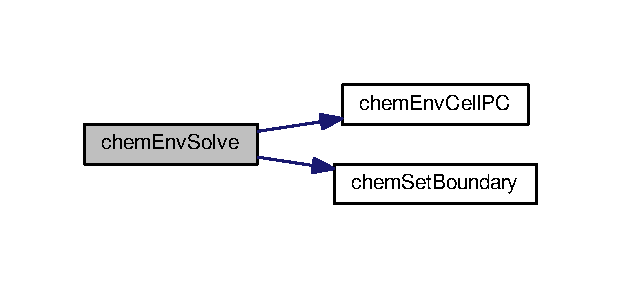
\includegraphics[width=298pt]{chemf_8c_a1f8f7d186d46aafcd792aaf3bee655a7_cgraph}
\end{center}
\end{figure}




Here is the caller graph for this function\-:\nopagebreak
\begin{figure}[H]
\begin{center}
\leavevmode
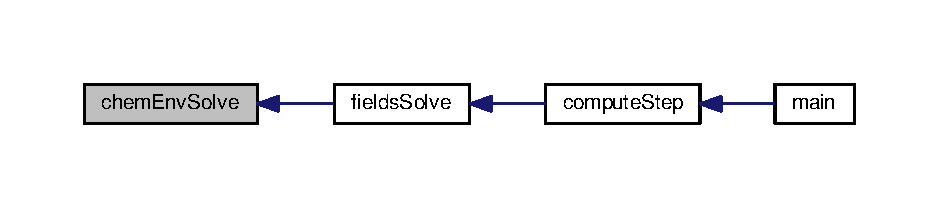
\includegraphics[width=350pt]{chemf_8c_a1f8f7d186d46aafcd792aaf3bee655a7_icgraph}
\end{center}
\end{figure}


\hypertarget{chemf_8c_afb692f34ea05262db93f9bf9590b06a7}{\index{chemf.\-c@{chemf.\-c}!chem\-Set\-Boundary@{chem\-Set\-Boundary}}
\index{chem\-Set\-Boundary@{chem\-Set\-Boundary}!chemf.c@{chemf.\-c}}
\subsubsection[{chem\-Set\-Boundary}]{\setlength{\rightskip}{0pt plus 5cm}void chem\-Set\-Boundary (
\begin{DoxyParamCaption}
\item[{int}]{coord, }
\item[{int}]{boundary}
\end{DoxyParamCaption}
)}}\label{chemf_8c_afb692f34ea05262db93f9bf9590b06a7}
This function sets boundary conditions for domain faces. 

Definition at line 75 of file chemf.\-c.



References bc\-Lower, bc\-Upper, chem\-Lower, and chem\-Upper.


\begin{DoxyCode}
76 \{
77   \textcolor{keywordflow}{if} (coord == 0 && boundary == -1) \{
78     \hyperlink{chemf_8c_a397798166a570960b5d468b6df8bf02c}{bcLower}[0] = \hyperlink{chemf_8c_a14199fec6ea96fe4a4c57bccaff2dfe7}{chemLower}[0];
79     \hyperlink{chemf_8c_aaea99b8c85fcedb15091dcac991999fd}{bcUpper}[0] = \hyperlink{chemf_8c_a14199fec6ea96fe4a4c57bccaff2dfe7}{chemLower}[0];
80     \hyperlink{chemf_8c_a397798166a570960b5d468b6df8bf02c}{bcLower}[1] = \hyperlink{chemf_8c_a14199fec6ea96fe4a4c57bccaff2dfe7}{chemLower}[1];
81     \hyperlink{chemf_8c_aaea99b8c85fcedb15091dcac991999fd}{bcUpper}[1] = \hyperlink{chemf_8c_a019f631b2e2795023bf22abef7d9f80e}{chemUpper}[1];
82     \hyperlink{chemf_8c_a397798166a570960b5d468b6df8bf02c}{bcLower}[2] = \hyperlink{chemf_8c_a14199fec6ea96fe4a4c57bccaff2dfe7}{chemLower}[2];
83     \hyperlink{chemf_8c_aaea99b8c85fcedb15091dcac991999fd}{bcUpper}[2] = \hyperlink{chemf_8c_a019f631b2e2795023bf22abef7d9f80e}{chemUpper}[2];
84   \}
85   \textcolor{keywordflow}{if} (coord == 0 && boundary == 1) \{
86     \hyperlink{chemf_8c_a397798166a570960b5d468b6df8bf02c}{bcLower}[0] = \hyperlink{chemf_8c_a019f631b2e2795023bf22abef7d9f80e}{chemUpper}[0];
87     \hyperlink{chemf_8c_aaea99b8c85fcedb15091dcac991999fd}{bcUpper}[0] = \hyperlink{chemf_8c_a019f631b2e2795023bf22abef7d9f80e}{chemUpper}[0];
88     \hyperlink{chemf_8c_a397798166a570960b5d468b6df8bf02c}{bcLower}[1] = \hyperlink{chemf_8c_a14199fec6ea96fe4a4c57bccaff2dfe7}{chemLower}[1];
89     \hyperlink{chemf_8c_aaea99b8c85fcedb15091dcac991999fd}{bcUpper}[1] = \hyperlink{chemf_8c_a019f631b2e2795023bf22abef7d9f80e}{chemUpper}[1];
90     \hyperlink{chemf_8c_a397798166a570960b5d468b6df8bf02c}{bcLower}[2] = \hyperlink{chemf_8c_a14199fec6ea96fe4a4c57bccaff2dfe7}{chemLower}[2];
91     \hyperlink{chemf_8c_aaea99b8c85fcedb15091dcac991999fd}{bcUpper}[2] = \hyperlink{chemf_8c_a019f631b2e2795023bf22abef7d9f80e}{chemUpper}[2];
92   \}
93   \textcolor{keywordflow}{if} (coord == 1 && boundary == -1) \{
94     \hyperlink{chemf_8c_a397798166a570960b5d468b6df8bf02c}{bcLower}[0] = \hyperlink{chemf_8c_a14199fec6ea96fe4a4c57bccaff2dfe7}{chemLower}[0];
95     \hyperlink{chemf_8c_aaea99b8c85fcedb15091dcac991999fd}{bcUpper}[0] = \hyperlink{chemf_8c_a019f631b2e2795023bf22abef7d9f80e}{chemUpper}[0];
96     \hyperlink{chemf_8c_a397798166a570960b5d468b6df8bf02c}{bcLower}[1] = \hyperlink{chemf_8c_a14199fec6ea96fe4a4c57bccaff2dfe7}{chemLower}[1];
97     \hyperlink{chemf_8c_aaea99b8c85fcedb15091dcac991999fd}{bcUpper}[1] = \hyperlink{chemf_8c_a14199fec6ea96fe4a4c57bccaff2dfe7}{chemLower}[1];
98     \hyperlink{chemf_8c_a397798166a570960b5d468b6df8bf02c}{bcLower}[2] = \hyperlink{chemf_8c_a14199fec6ea96fe4a4c57bccaff2dfe7}{chemLower}[2];
99     \hyperlink{chemf_8c_aaea99b8c85fcedb15091dcac991999fd}{bcUpper}[2] = \hyperlink{chemf_8c_a019f631b2e2795023bf22abef7d9f80e}{chemUpper}[2];
100   \}
101   \textcolor{keywordflow}{if} (coord == 1 && boundary == 1) \{
102     \hyperlink{chemf_8c_a397798166a570960b5d468b6df8bf02c}{bcLower}[0] = \hyperlink{chemf_8c_a14199fec6ea96fe4a4c57bccaff2dfe7}{chemLower}[0];
103     \hyperlink{chemf_8c_aaea99b8c85fcedb15091dcac991999fd}{bcUpper}[0] = \hyperlink{chemf_8c_a019f631b2e2795023bf22abef7d9f80e}{chemUpper}[0];
104     \hyperlink{chemf_8c_a397798166a570960b5d468b6df8bf02c}{bcLower}[1] = \hyperlink{chemf_8c_a019f631b2e2795023bf22abef7d9f80e}{chemUpper}[1];
105     \hyperlink{chemf_8c_aaea99b8c85fcedb15091dcac991999fd}{bcUpper}[1] = \hyperlink{chemf_8c_a019f631b2e2795023bf22abef7d9f80e}{chemUpper}[1];
106     \hyperlink{chemf_8c_a397798166a570960b5d468b6df8bf02c}{bcLower}[2] = \hyperlink{chemf_8c_a14199fec6ea96fe4a4c57bccaff2dfe7}{chemLower}[2];
107     \hyperlink{chemf_8c_aaea99b8c85fcedb15091dcac991999fd}{bcUpper}[2] = \hyperlink{chemf_8c_a019f631b2e2795023bf22abef7d9f80e}{chemUpper}[2];
108   \}
109   \textcolor{keywordflow}{if} (coord == 2 && boundary == -1) \{
110     \hyperlink{chemf_8c_a397798166a570960b5d468b6df8bf02c}{bcLower}[0] = \hyperlink{chemf_8c_a14199fec6ea96fe4a4c57bccaff2dfe7}{chemLower}[0];
111     \hyperlink{chemf_8c_aaea99b8c85fcedb15091dcac991999fd}{bcUpper}[0] = \hyperlink{chemf_8c_a019f631b2e2795023bf22abef7d9f80e}{chemUpper}[0];
112     \hyperlink{chemf_8c_a397798166a570960b5d468b6df8bf02c}{bcLower}[1] = \hyperlink{chemf_8c_a14199fec6ea96fe4a4c57bccaff2dfe7}{chemLower}[1];
113     \hyperlink{chemf_8c_aaea99b8c85fcedb15091dcac991999fd}{bcUpper}[1] = \hyperlink{chemf_8c_a019f631b2e2795023bf22abef7d9f80e}{chemUpper}[1];
114     \hyperlink{chemf_8c_a397798166a570960b5d468b6df8bf02c}{bcLower}[2] = \hyperlink{chemf_8c_a14199fec6ea96fe4a4c57bccaff2dfe7}{chemLower}[2];
115     \hyperlink{chemf_8c_aaea99b8c85fcedb15091dcac991999fd}{bcUpper}[2] = \hyperlink{chemf_8c_a14199fec6ea96fe4a4c57bccaff2dfe7}{chemLower}[2];
116   \}
117   \textcolor{keywordflow}{if} (coord == 2 && boundary == 1) \{
118     \hyperlink{chemf_8c_a397798166a570960b5d468b6df8bf02c}{bcLower}[0] = \hyperlink{chemf_8c_a14199fec6ea96fe4a4c57bccaff2dfe7}{chemLower}[0];
119     \hyperlink{chemf_8c_aaea99b8c85fcedb15091dcac991999fd}{bcUpper}[0] = \hyperlink{chemf_8c_a019f631b2e2795023bf22abef7d9f80e}{chemUpper}[0];
120     \hyperlink{chemf_8c_a397798166a570960b5d468b6df8bf02c}{bcLower}[1] = \hyperlink{chemf_8c_a14199fec6ea96fe4a4c57bccaff2dfe7}{chemLower}[1];
121     \hyperlink{chemf_8c_aaea99b8c85fcedb15091dcac991999fd}{bcUpper}[1] = \hyperlink{chemf_8c_a019f631b2e2795023bf22abef7d9f80e}{chemUpper}[1];
122     \hyperlink{chemf_8c_a397798166a570960b5d468b6df8bf02c}{bcLower}[2] = \hyperlink{chemf_8c_a019f631b2e2795023bf22abef7d9f80e}{chemUpper}[2];
123     \hyperlink{chemf_8c_aaea99b8c85fcedb15091dcac991999fd}{bcUpper}[2] = \hyperlink{chemf_8c_a019f631b2e2795023bf22abef7d9f80e}{chemUpper}[2];
124   \}
125 \}
\end{DoxyCode}


Here is the caller graph for this function\-:\nopagebreak
\begin{figure}[H]
\begin{center}
\leavevmode
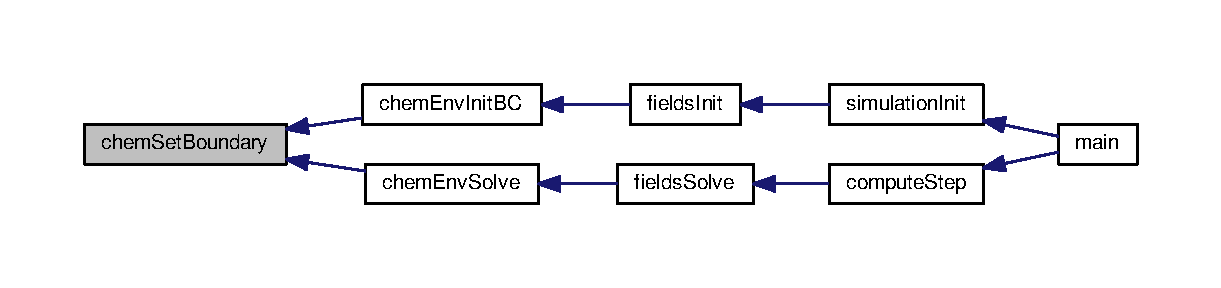
\includegraphics[width=350pt]{chemf_8c_afb692f34ea05262db93f9bf9590b06a7_icgraph}
\end{center}
\end{figure}




\subsection{Variable Documentation}
\hypertarget{chemf_8c_a397798166a570960b5d468b6df8bf02c}{\index{chemf.\-c@{chemf.\-c}!bc\-Lower@{bc\-Lower}}
\index{bc\-Lower@{bc\-Lower}!chemf.c@{chemf.\-c}}
\subsubsection[{bc\-Lower}]{\setlength{\rightskip}{0pt plus 5cm}long long bc\-Lower\mbox{[}3\mbox{]}}}\label{chemf_8c_a397798166a570960b5d468b6df8bf02c}


Definition at line 54 of file chemf.\-c.

\hypertarget{chemf_8c_aaea99b8c85fcedb15091dcac991999fd}{\index{chemf.\-c@{chemf.\-c}!bc\-Upper@{bc\-Upper}}
\index{bc\-Upper@{bc\-Upper}!chemf.c@{chemf.\-c}}
\subsubsection[{bc\-Upper}]{\setlength{\rightskip}{0pt plus 5cm}long long bc\-Upper\mbox{[}3\mbox{]}}}\label{chemf_8c_aaea99b8c85fcedb15091dcac991999fd}


Definition at line 55 of file chemf.\-c.

\hypertarget{chemf_8c_ad634e858729e0c04e8b9a4b0a1144b10}{\index{chemf.\-c@{chemf.\-c}!chem\-A@{chem\-A}}
\index{chem\-A@{chem\-A}!chemf.c@{chemf.\-c}}
\subsubsection[{chem\-A}]{\setlength{\rightskip}{0pt plus 5cm}H\-Y\-P\-R\-E\-\_\-\-S\-Struct\-Matrix chem\-A\mbox{[}{\bf N\-C\-H\-E\-M}\mbox{]}}}\label{chemf_8c_ad634e858729e0c04e8b9a4b0a1144b10}


Definition at line 40 of file chemf.\-c.

\hypertarget{chemf_8c_afb43e9c9d8160250a03e1b41902473fd}{\index{chemf.\-c@{chemf.\-c}!chemb@{chemb}}
\index{chemb@{chemb}!chemf.c@{chemf.\-c}}
\subsubsection[{chemb}]{\setlength{\rightskip}{0pt plus 5cm}H\-Y\-P\-R\-E\-\_\-\-S\-Struct\-Vector chemb\mbox{[}{\bf N\-C\-H\-E\-M}\mbox{]}}}\label{chemf_8c_afb43e9c9d8160250a03e1b41902473fd}


Definition at line 41 of file chemf.\-c.

\hypertarget{chemf_8c_aaac58de32c5dda56ce31654ec3e19337}{\index{chemf.\-c@{chemf.\-c}!chem\-Graph@{chem\-Graph}}
\index{chem\-Graph@{chem\-Graph}!chemf.c@{chemf.\-c}}
\subsubsection[{chem\-Graph}]{\setlength{\rightskip}{0pt plus 5cm}H\-Y\-P\-R\-E\-\_\-\-S\-Struct\-Graph chem\-Graph\mbox{[}{\bf N\-C\-H\-E\-M}\mbox{]}}}\label{chemf_8c_aaac58de32c5dda56ce31654ec3e19337}


Definition at line 37 of file chemf.\-c.

\hypertarget{chemf_8c_ad7a28a5fc279e8b757bdc6a4b57c25be}{\index{chemf.\-c@{chemf.\-c}!chem\-Grid@{chem\-Grid}}
\index{chem\-Grid@{chem\-Grid}!chemf.c@{chemf.\-c}}
\subsubsection[{chem\-Grid}]{\setlength{\rightskip}{0pt plus 5cm}H\-Y\-P\-R\-E\-\_\-\-S\-Struct\-Grid chem\-Grid\mbox{[}{\bf N\-C\-H\-E\-M}\mbox{]}}}\label{chemf_8c_ad7a28a5fc279e8b757bdc6a4b57c25be}


Definition at line 36 of file chemf.\-c.

\hypertarget{chemf_8c_a26adfe146e722023d7f81bf278bde9e7}{\index{chemf.\-c@{chemf.\-c}!chem\-Iter@{chem\-Iter}}
\index{chem\-Iter@{chem\-Iter}!chemf.c@{chemf.\-c}}
\subsubsection[{chem\-Iter}]{\setlength{\rightskip}{0pt plus 5cm}int chem\-Iter\mbox{[}{\bf N\-C\-H\-E\-M}\mbox{]}}}\label{chemf_8c_a26adfe146e722023d7f81bf278bde9e7}


Definition at line 62 of file chemf.\-c.

\hypertarget{chemf_8c_ab35147d777155659aaad43553e3378f4}{\index{chemf.\-c@{chemf.\-c}!chem\-Lambda@{chem\-Lambda}}
\index{chem\-Lambda@{chem\-Lambda}!chemf.c@{chemf.\-c}}
\subsubsection[{chem\-Lambda}]{\setlength{\rightskip}{0pt plus 5cm}double chem\-Lambda = 0.\-25}}\label{chemf_8c_ab35147d777155659aaad43553e3378f4}


Definition at line 58 of file chemf.\-c.

\hypertarget{chemf_8c_a14199fec6ea96fe4a4c57bccaff2dfe7}{\index{chemf.\-c@{chemf.\-c}!chem\-Lower@{chem\-Lower}}
\index{chem\-Lower@{chem\-Lower}!chemf.c@{chemf.\-c}}
\subsubsection[{chem\-Lower}]{\setlength{\rightskip}{0pt plus 5cm}long long chem\-Lower\mbox{[}3\mbox{]}}}\label{chemf_8c_a14199fec6ea96fe4a4c57bccaff2dfe7}


Definition at line 53 of file chemf.\-c.

\hypertarget{chemf_8c_a242fb3ba38fb1c6054fd05507394f08b}{\index{chemf.\-c@{chemf.\-c}!chem\-Object\-Type@{chem\-Object\-Type}}
\index{chem\-Object\-Type@{chem\-Object\-Type}!chemf.c@{chemf.\-c}}
\subsubsection[{chem\-Object\-Type}]{\setlength{\rightskip}{0pt plus 5cm}int chem\-Object\-Type}}\label{chemf_8c_a242fb3ba38fb1c6054fd05507394f08b}


Definition at line 51 of file chemf.\-c.

\hypertarget{chemf_8c_a998a7ebb65eb001abcee46c1ea1b1756}{\index{chemf.\-c@{chemf.\-c}!chem\-Par\-A@{chem\-Par\-A}}
\index{chem\-Par\-A@{chem\-Par\-A}!chemf.c@{chemf.\-c}}
\subsubsection[{chem\-Par\-A}]{\setlength{\rightskip}{0pt plus 5cm}H\-Y\-P\-R\-E\-\_\-\-Par\-C\-S\-R\-Matrix chem\-Par\-A\mbox{[}{\bf N\-C\-H\-E\-M}\mbox{]}}}\label{chemf_8c_a998a7ebb65eb001abcee46c1ea1b1756}


Definition at line 44 of file chemf.\-c.

\hypertarget{chemf_8c_af74b7f36ec77fb8e0638db98dd2ee47a}{\index{chemf.\-c@{chemf.\-c}!chem\-Parb@{chem\-Parb}}
\index{chem\-Parb@{chem\-Parb}!chemf.c@{chemf.\-c}}
\subsubsection[{chem\-Parb}]{\setlength{\rightskip}{0pt plus 5cm}H\-Y\-P\-R\-E\-\_\-\-Par\-Vector chem\-Parb\mbox{[}{\bf N\-C\-H\-E\-M}\mbox{]}}}\label{chemf_8c_af74b7f36ec77fb8e0638db98dd2ee47a}


Definition at line 45 of file chemf.\-c.

\hypertarget{chemf_8c_aae118f98b57f3dda9f036d39db247bb1}{\index{chemf.\-c@{chemf.\-c}!chem\-Parx@{chem\-Parx}}
\index{chem\-Parx@{chem\-Parx}!chemf.c@{chemf.\-c}}
\subsubsection[{chem\-Parx}]{\setlength{\rightskip}{0pt plus 5cm}H\-Y\-P\-R\-E\-\_\-\-Par\-Vector chem\-Parx\mbox{[}{\bf N\-C\-H\-E\-M}\mbox{]}}}\label{chemf_8c_aae118f98b57f3dda9f036d39db247bb1}


Definition at line 46 of file chemf.\-c.

\hypertarget{chemf_8c_a614434a804d9a302d1db9603c22b60a7}{\index{chemf.\-c@{chemf.\-c}!chem\-P\-C@{chem\-P\-C}}
\index{chem\-P\-C@{chem\-P\-C}!chemf.c@{chemf.\-c}}
\subsubsection[{chem\-P\-C}]{\setlength{\rightskip}{0pt plus 5cm}double$\ast$ chem\-P\-C}}\label{chemf_8c_a614434a804d9a302d1db9603c22b60a7}


Definition at line 70 of file chemf.\-c.

\hypertarget{chemf_8c_a91747632f47bf551e8915e343439777f}{\index{chemf.\-c@{chemf.\-c}!chem\-Precond@{chem\-Precond}}
\index{chem\-Precond@{chem\-Precond}!chemf.c@{chemf.\-c}}
\subsubsection[{chem\-Precond}]{\setlength{\rightskip}{0pt plus 5cm}H\-Y\-P\-R\-E\-\_\-\-Solver chem\-Precond\mbox{[}{\bf N\-C\-H\-E\-M}\mbox{]}}}\label{chemf_8c_a91747632f47bf551e8915e343439777f}


Definition at line 49 of file chemf.\-c.

\hypertarget{chemf_8c_a99bbb7b0352d9c850e98287fa45b42c0}{\index{chemf.\-c@{chemf.\-c}!chem\-Solver@{chem\-Solver}}
\index{chem\-Solver@{chem\-Solver}!chemf.c@{chemf.\-c}}
\subsubsection[{chem\-Solver}]{\setlength{\rightskip}{0pt plus 5cm}H\-Y\-P\-R\-E\-\_\-\-Solver chem\-Solver\mbox{[}{\bf N\-C\-H\-E\-M}\mbox{]}}}\label{chemf_8c_a99bbb7b0352d9c850e98287fa45b42c0}


Definition at line 48 of file chemf.\-c.

\hypertarget{chemf_8c_ae8a36b5c7c6256a7d248a08c71944c73}{\index{chemf.\-c@{chemf.\-c}!chem\-Stencil@{chem\-Stencil}}
\index{chem\-Stencil@{chem\-Stencil}!chemf.c@{chemf.\-c}}
\subsubsection[{chem\-Stencil}]{\setlength{\rightskip}{0pt plus 5cm}H\-Y\-P\-R\-E\-\_\-\-S\-Struct\-Stencil chem\-Stencil\mbox{[}{\bf N\-C\-H\-E\-M}\mbox{]}}}\label{chemf_8c_ae8a36b5c7c6256a7d248a08c71944c73}


Definition at line 38 of file chemf.\-c.

\hypertarget{chemf_8c_a019f631b2e2795023bf22abef7d9f80e}{\index{chemf.\-c@{chemf.\-c}!chem\-Upper@{chem\-Upper}}
\index{chem\-Upper@{chem\-Upper}!chemf.c@{chemf.\-c}}
\subsubsection[{chem\-Upper}]{\setlength{\rightskip}{0pt plus 5cm}long long chem\-Upper\mbox{[}3\mbox{]}}}\label{chemf_8c_a019f631b2e2795023bf22abef7d9f80e}


Definition at line 53 of file chemf.\-c.

\hypertarget{chemf_8c_aa73fdbffdd3d43dd503718011b98e41f}{\index{chemf.\-c@{chemf.\-c}!chem\-Vartypes@{chem\-Vartypes}}
\index{chem\-Vartypes@{chem\-Vartypes}!chemf.c@{chemf.\-c}}
\subsubsection[{chem\-Vartypes}]{\setlength{\rightskip}{0pt plus 5cm}H\-Y\-P\-R\-E\-\_\-\-S\-Struct\-Variable chem\-Vartypes\mbox{[}1\mbox{]} = \{ H\-Y\-P\-R\-E\-\_\-\-S\-S\-T\-R\-U\-C\-T\-\_\-\-V\-A\-R\-I\-A\-B\-L\-E\-\_\-\-N\-O\-D\-E \}}}\label{chemf_8c_aa73fdbffdd3d43dd503718011b98e41f}


Definition at line 66 of file chemf.\-c.

\hypertarget{chemf_8c_a48c5bcbe8787c6a6be2a6d5bcdae101f}{\index{chemf.\-c@{chemf.\-c}!chemx@{chemx}}
\index{chemx@{chemx}!chemf.c@{chemf.\-c}}
\subsubsection[{chemx}]{\setlength{\rightskip}{0pt plus 5cm}H\-Y\-P\-R\-E\-\_\-\-S\-Struct\-Vector chemx\mbox{[}{\bf N\-C\-H\-E\-M}\mbox{]}}}\label{chemf_8c_a48c5bcbe8787c6a6be2a6d5bcdae101f}


Definition at line 42 of file chemf.\-c.

\hypertarget{chemf_8c_ad1178dce1f62833a078c63e911e2e023}{\index{chemf.\-c@{chemf.\-c}!chem\-Z@{chem\-Z}}
\index{chem\-Z@{chem\-Z}!chemf.c@{chemf.\-c}}
\subsubsection[{chem\-Z}]{\setlength{\rightskip}{0pt plus 5cm}double chem\-Z\mbox{[}{\bf N\-C\-H\-E\-M}\mbox{]}}}\label{chemf_8c_ad1178dce1f62833a078c63e911e2e023}


Definition at line 64 of file chemf.\-c.

\hypertarget{chemf_8c_a27dc1f70b41e3739d1629663a1d3d0a6}{\index{chemf.\-c@{chemf.\-c}!chfname@{chfname}}
\index{chfname@{chfname}!chemf.c@{chemf.\-c}}
\subsubsection[{chfname}]{\setlength{\rightskip}{0pt plus 5cm}char chfname\mbox{[}256\mbox{]}}}\label{chemf_8c_a27dc1f70b41e3739d1629663a1d3d0a6}


Definition at line 60 of file chemf.\-c.

\hypertarget{chemf_8c_a881c8c944ac83a5c022ee0e236f35e52}{\index{chemf.\-c@{chemf.\-c}!dt@{dt}}
\index{dt@{dt}!chemf.c@{chemf.\-c}}
\subsubsection[{dt}]{\setlength{\rightskip}{0pt plus 5cm}double dt\mbox{[}{\bf N\-C\-H\-E\-M}\mbox{]}}}\label{chemf_8c_a881c8c944ac83a5c022ee0e236f35e52}


Definition at line 57 of file chemf.\-c.

\hypertarget{chemf_8c_a07fef4b421caa5300b13b2ba89422841}{\index{chemf.\-c@{chemf.\-c}!number\-Of\-Iters@{number\-Of\-Iters}}
\index{number\-Of\-Iters@{number\-Of\-Iters}!chemf.c@{chemf.\-c}}
\subsubsection[{number\-Of\-Iters}]{\setlength{\rightskip}{0pt plus 5cm}int number\-Of\-Iters}}\label{chemf_8c_a07fef4b421caa5300b13b2ba89422841}


Definition at line 68 of file chemf.\-c.


\hypertarget{comm_8c}{\section{comm.\-c File Reference}
\label{comm_8c}\index{comm.\-c@{comm.\-c}}
}


contains communication functions  


{\ttfamily \#include $<$stdlib.\-h$>$}\\*
{\ttfamily \#include \char`\"{}global.\-h\char`\"{}}\\*
Include dependency graph for comm.\-c\-:\nopagebreak
\begin{figure}[H]
\begin{center}
\leavevmode
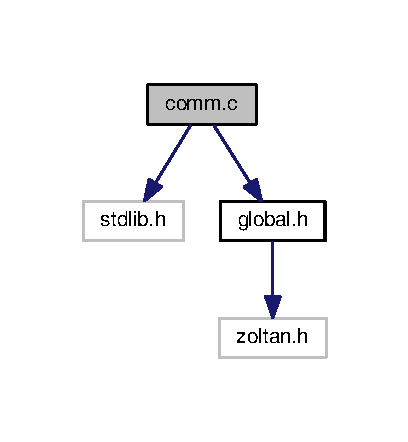
\includegraphics[width=196pt]{comm_8c__incl}
\end{center}
\end{figure}
\subsection*{Data Structures}
\begin{DoxyCompactItemize}
\item 
struct \hyperlink{structexpData}{exp\-Data}
\end{DoxyCompactItemize}
\subsection*{Macros}
\begin{DoxyCompactItemize}
\item 
\#define \hyperlink{comm_8c_a93da5acfae81b763e797f8562d49ca64}{M\-A\-X\-\_\-\-E\-X\-P\-O\-R\-T\-E\-D\-\_\-\-P\-E\-R\-\_\-\-P\-R\-O\-C}~2$\ast$\hyperlink{global_8h_a2de426dd266cfdaaf6fb52ba3dc2740a}{max\-Cells\-Per\-Proc}
\end{DoxyCompactItemize}
\subsection*{Functions}
\begin{DoxyCompactItemize}
\item 
int \hyperlink{comm_8c_a0a0b21ecf1a24a3cae73074d6bf6c68e}{comm\-\_\-compare\-\_\-exp\-\_\-list} (const void $\ast$a, const void $\ast$\hyperlink{tempf_8c_a74a523afdfebddf9b6b280e545977c5a}{b})
\item 
void \hyperlink{comm_8c_a191bffd6b8283bf118dec0d0422fa2b3}{create\-Export\-List} ()
\item 
void \hyperlink{comm_8c_abdd72f1d40c6c4bf47ad78c4f3c349d5}{comm\-Cleanup} ()
\item 
void \hyperlink{comm_8c_aa92fc6732720bc9accbbdef7fb02384f}{cells\-Exchange\-Init} ()
\item 
void \hyperlink{comm_8c_ac5b7dbd1157ef088c4e6f8a9f08fcc4b}{cells\-Exchange\-Wait} ()
\item 
void \hyperlink{comm_8c_a206e073b7e35f281184b3487b3bbc055}{dens\-Pot\-Exchange\-Init} ()
\item 
void \hyperlink{comm_8c_afebf59220f4170178e5fb828d569aaab}{dens\-Pot\-Exchange\-Wait} ()
\end{DoxyCompactItemize}
\subsection*{Variables}
\begin{DoxyCompactItemize}
\item 
M\-P\-I\-\_\-\-Request $\ast$ \hyperlink{comm_8c_a827e028e778c94dd2e816ae6077a3198}{req\-Send}
\item 
M\-P\-I\-\_\-\-Request $\ast$ \hyperlink{comm_8c_ad7a9f44424272a25979b199886bdce73}{req\-Recv}
\item 
int64\-\_\-t $\ast$ \hyperlink{comm_8c_a16d801f1b7f6a598f31107a146b11f16}{send\-Offset}
\item 
int64\-\_\-t $\ast$ \hyperlink{comm_8c_a4f0cc30ef1f6185ba3d6406343e1a574}{recv\-Offset}
\item 
struct \hyperlink{structexpData}{exp\-Data} $\ast$ \hyperlink{comm_8c_a6f7e234508139d1113a2f60a1b36c04a}{exp\-List}
\item 
int $\ast$ \hyperlink{comm_8c_a073b7079fe649b9ae1b5c4056ccaa4fb}{recv\-Count}
\item 
int $\ast$ \hyperlink{comm_8c_aed19f012b3fe7ae1966dcc8b89cdf7b2}{send\-Count}
\end{DoxyCompactItemize}


\subsection{Detailed Description}
contains communication functions 

Definition in file \hyperlink{comm_8c_source}{comm.\-c}.



\subsection{Macro Definition Documentation}
\hypertarget{comm_8c_a93da5acfae81b763e797f8562d49ca64}{\index{comm.\-c@{comm.\-c}!M\-A\-X\-\_\-\-E\-X\-P\-O\-R\-T\-E\-D\-\_\-\-P\-E\-R\-\_\-\-P\-R\-O\-C@{M\-A\-X\-\_\-\-E\-X\-P\-O\-R\-T\-E\-D\-\_\-\-P\-E\-R\-\_\-\-P\-R\-O\-C}}
\index{M\-A\-X\-\_\-\-E\-X\-P\-O\-R\-T\-E\-D\-\_\-\-P\-E\-R\-\_\-\-P\-R\-O\-C@{M\-A\-X\-\_\-\-E\-X\-P\-O\-R\-T\-E\-D\-\_\-\-P\-E\-R\-\_\-\-P\-R\-O\-C}!comm.c@{comm.\-c}}
\subsubsection[{M\-A\-X\-\_\-\-E\-X\-P\-O\-R\-T\-E\-D\-\_\-\-P\-E\-R\-\_\-\-P\-R\-O\-C}]{\setlength{\rightskip}{0pt plus 5cm}\#define M\-A\-X\-\_\-\-E\-X\-P\-O\-R\-T\-E\-D\-\_\-\-P\-E\-R\-\_\-\-P\-R\-O\-C~2$\ast${\bf max\-Cells\-Per\-Proc}}}\label{comm_8c_a93da5acfae81b763e797f8562d49ca64}


Definition at line 48 of file comm.\-c.



\subsection{Function Documentation}
\hypertarget{comm_8c_aa92fc6732720bc9accbbdef7fb02384f}{\index{comm.\-c@{comm.\-c}!cells\-Exchange\-Init@{cells\-Exchange\-Init}}
\index{cells\-Exchange\-Init@{cells\-Exchange\-Init}!comm.c@{comm.\-c}}
\subsubsection[{cells\-Exchange\-Init}]{\setlength{\rightskip}{0pt plus 5cm}void cells\-Exchange\-Init (
\begin{DoxyParamCaption}
{}
\end{DoxyParamCaption}
)}}\label{comm_8c_aa92fc6732720bc9accbbdef7fb02384f}
This function initiate sending and receiving cells' data between processes. 

Definition at line 182 of file comm.\-c.



References exp\-Data\-::cell, cells, cell\-Data\-::ctype, part\-Data\-::ctype, part\-Data\-::h, h, lnc, M\-P\-Irank, M\-P\-Isize, nc, num\-Exp, num\-Imp, recv\-Count, recv\-Data, recv\-Offset, req\-Recv, req\-Send, send\-Count, send\-Data, send\-Offset, cell\-Data\-::size, part\-Data\-::size, tlnc, cell\-Data\-::x, part\-Data\-::x, cell\-Data\-::y, part\-Data\-::y, part\-Data\-::young, cell\-Data\-::z, and part\-Data\-::z.


\begin{DoxyCode}
183 \{
184   \textcolor{keywordtype}{int} i;
185 
186   \textcolor{keywordflow}{if} (\hyperlink{global_8h_a0845b4b004824f1fe3cd69db1672fa15}{nc} < \hyperlink{global_8h_a0d7d02544d01ceac87c9d5cadc3af0df}{MPIsize} || \hyperlink{global_8h_a0d7d02544d01ceac87c9d5cadc3af0df}{MPIsize} == 1)
187     \textcolor{keywordflow}{return};
188 
189   \textcolor{comment}{/* allocate communication buffers */}
190   \hyperlink{global_8h_ac928fbed09198ca6c116fb58a115b594}{sendData} = (\textcolor{keyword}{struct }\hyperlink{structpartData}{partData} *) malloc(\hyperlink{global_8h_a4c3c9a79704128f7fcc9ebf4bdd9e3fc}{numExp} * \textcolor{keyword}{sizeof}(\textcolor{keyword}{struct} 
      \hyperlink{structpartData}{partData}));
191 \textcolor{preprocessor}{#ifdef \_\_MIC\_\_}
192 \textcolor{preprocessor}{}  \hyperlink{global_8h_a9909963356d98bc262c21fed8a950cc2}{recvData} = (\textcolor{keyword}{struct }\hyperlink{structpartData}{partData} *) \_mm\_malloc(\hyperlink{global_8h_a07792d8e2788e030124304f47e8cf1f6}{numImp} * \textcolor{keyword}{sizeof}(\textcolor{keyword}{struct} 
      \hyperlink{structpartData}{partData}),64);
193 \textcolor{preprocessor}{#else}
194 \textcolor{preprocessor}{}  \hyperlink{global_8h_a9909963356d98bc262c21fed8a950cc2}{recvData} = (\textcolor{keyword}{struct }\hyperlink{structpartData}{partData} *) malloc(\hyperlink{global_8h_a07792d8e2788e030124304f47e8cf1f6}{numImp} * \textcolor{keyword}{sizeof}(\textcolor{keyword}{struct} 
      \hyperlink{structpartData}{partData}));
195 \textcolor{preprocessor}{#endif}
196 \textcolor{preprocessor}{}  \hyperlink{comm_8c_a827e028e778c94dd2e816ae6077a3198}{reqSend} = (MPI\_Request *) malloc(\textcolor{keyword}{sizeof}(MPI\_Request) * \hyperlink{global_8h_a0d7d02544d01ceac87c9d5cadc3af0df}{MPIsize});
197   \hyperlink{comm_8c_ad7a9f44424272a25979b199886bdce73}{reqRecv} = (MPI\_Request *) malloc(\textcolor{keyword}{sizeof}(MPI\_Request) * \hyperlink{global_8h_a0d7d02544d01ceac87c9d5cadc3af0df}{MPIsize});
198 
199   \textcolor{comment}{/* create reduced particle data buffer for exporting */}
200   \textcolor{keywordflow}{for} (i = 0; i < \hyperlink{global_8h_a4c3c9a79704128f7fcc9ebf4bdd9e3fc}{numExp}; i++) \{
201     \hyperlink{global_8h_ac928fbed09198ca6c116fb58a115b594}{sendData}[i].\hyperlink{structpartData_af88b946fb90d5f08b5fb740c70e98c10}{x} = \hyperlink{global_8h_a3ea537bde8d64e54770a2bd81e3f00be}{cells}[\hyperlink{comm_8c_a6f7e234508139d1113a2f60a1b36c04a}{expList}[i].\hyperlink{structexpData_af00601a22186810a9e6d16efb75862ce}{cell}].\hyperlink{structcellData_af88b946fb90d5f08b5fb740c70e98c10}{x};
202     \hyperlink{global_8h_ac928fbed09198ca6c116fb58a115b594}{sendData}[i].\hyperlink{structpartData_ab927965981178aa1fba979a37168db2a}{y} = \hyperlink{global_8h_a3ea537bde8d64e54770a2bd81e3f00be}{cells}[\hyperlink{comm_8c_a6f7e234508139d1113a2f60a1b36c04a}{expList}[i].\hyperlink{structexpData_af00601a22186810a9e6d16efb75862ce}{cell}].\hyperlink{structcellData_ab927965981178aa1fba979a37168db2a}{y};
203     \hyperlink{global_8h_ac928fbed09198ca6c116fb58a115b594}{sendData}[i].\hyperlink{structpartData_ab3e6ed577a7c669c19de1f9c1b46c872}{z} = \hyperlink{global_8h_a3ea537bde8d64e54770a2bd81e3f00be}{cells}[\hyperlink{comm_8c_a6f7e234508139d1113a2f60a1b36c04a}{expList}[i].\hyperlink{structexpData_af00601a22186810a9e6d16efb75862ce}{cell}].\hyperlink{structcellData_ab3e6ed577a7c669c19de1f9c1b46c872}{z};
204     \hyperlink{global_8h_ac928fbed09198ca6c116fb58a115b594}{sendData}[i].\hyperlink{structpartData_aba3c5d750d5dbd6e86c11ecaca62885e}{size} = \hyperlink{global_8h_a3ea537bde8d64e54770a2bd81e3f00be}{cells}[\hyperlink{comm_8c_a6f7e234508139d1113a2f60a1b36c04a}{expList}[i].\hyperlink{structexpData_af00601a22186810a9e6d16efb75862ce}{cell}].\hyperlink{structcellData_aba3c5d750d5dbd6e86c11ecaca62885e}{size};
205     \hyperlink{global_8h_ac928fbed09198ca6c116fb58a115b594}{sendData}[i].\hyperlink{structpartData_a8ee9be1b5aa75abae556de3088cba6d9}{h} = \hyperlink{global_8h_adae58efd3b7d9072a77aff9c63040d05}{h};
206     \hyperlink{global_8h_ac928fbed09198ca6c116fb58a115b594}{sendData}[i].\hyperlink{structpartData_a47ec3689b1fd89ba8e75d9a9975ba63f}{young} = (double) \hyperlink{global_8h_a3ea537bde8d64e54770a2bd81e3f00be}{cells}[\hyperlink{comm_8c_a6f7e234508139d1113a2f60a1b36c04a}{expList}[i].cell].
      \hyperlink{structpartData_a47ec3689b1fd89ba8e75d9a9975ba63f}{young};
207     \hyperlink{global_8h_ac928fbed09198ca6c116fb58a115b594}{sendData}[i].\hyperlink{structpartData_a13fbf3c17594503f639a7ef768ea73bb}{ctype} = \hyperlink{global_8h_a3ea537bde8d64e54770a2bd81e3f00be}{cells}[\hyperlink{comm_8c_a6f7e234508139d1113a2f60a1b36c04a}{expList}[i].\hyperlink{structexpData_af00601a22186810a9e6d16efb75862ce}{cell}].
      \hyperlink{structcellData_a13fbf3c17594503f639a7ef768ea73bb}{ctype};
208   \}
209 
210   \textcolor{comment}{/* send cells - asynchronous MPI call */}
211   \textcolor{keywordflow}{for} (i = 0; i < \hyperlink{global_8h_a0d7d02544d01ceac87c9d5cadc3af0df}{MPIsize}; i++) \{
212     \textcolor{keywordflow}{if} (\hyperlink{comm_8c_aed19f012b3fe7ae1966dcc8b89cdf7b2}{sendCount}[i] == 0 || \hyperlink{global_8h_ac3c96b975a3376c555ad22a7d2688b2f}{tlnc}[i] == 0 || \hyperlink{global_8h_a7065c019590815f10169c219f358e7d0}{lnc} == 0)
213       \textcolor{keywordflow}{continue};
214     MPI\_Isend(&\hyperlink{global_8h_ac928fbed09198ca6c116fb58a115b594}{sendData}[\hyperlink{comm_8c_a16d801f1b7f6a598f31107a146b11f16}{sendOffset}[i]],
215               \hyperlink{comm_8c_aed19f012b3fe7ae1966dcc8b89cdf7b2}{sendCount}[i] * \textcolor{keyword}{sizeof}(\textcolor{keyword}{struct} \hyperlink{structpartData}{partData}), MPI\_BYTE, i, 
      \hyperlink{global_8h_a710288ab7d2734acc4566a87a645325d}{MPIrank},
216               MPI\_COMM\_WORLD, &\hyperlink{comm_8c_a827e028e778c94dd2e816ae6077a3198}{reqSend}[i]);
217   \}
218 
219   \textcolor{comment}{/* receive cells - asynchronous MPI call */}
220   \textcolor{keywordflow}{for} (i = 0; i < \hyperlink{global_8h_a0d7d02544d01ceac87c9d5cadc3af0df}{MPIsize}; i++) \{
221     \textcolor{keywordflow}{if} (\hyperlink{comm_8c_a073b7079fe649b9ae1b5c4056ccaa4fb}{recvCount}[i] == 0 || \hyperlink{global_8h_ac3c96b975a3376c555ad22a7d2688b2f}{tlnc}[i] == 0 || \hyperlink{global_8h_a7065c019590815f10169c219f358e7d0}{lnc} == 0)
222       \textcolor{keywordflow}{continue};
223     MPI\_Irecv(&\hyperlink{global_8h_a9909963356d98bc262c21fed8a950cc2}{recvData}[\hyperlink{comm_8c_a4f0cc30ef1f6185ba3d6406343e1a574}{recvOffset}[i]],
224               \hyperlink{comm_8c_a073b7079fe649b9ae1b5c4056ccaa4fb}{recvCount}[i] * \textcolor{keyword}{sizeof}(\textcolor{keyword}{struct} \hyperlink{structpartData}{partData}), MPI\_BYTE, i, i,
225               MPI\_COMM\_WORLD, &\hyperlink{comm_8c_ad7a9f44424272a25979b199886bdce73}{reqRecv}[i]);
226   \}
227 
228 \}
\end{DoxyCode}


Here is the caller graph for this function\-:\nopagebreak
\begin{figure}[H]
\begin{center}
\leavevmode
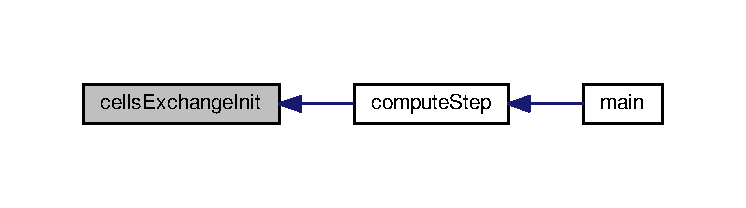
\includegraphics[width=350pt]{comm_8c_aa92fc6732720bc9accbbdef7fb02384f_icgraph}
\end{center}
\end{figure}


\hypertarget{comm_8c_ac5b7dbd1157ef088c4e6f8a9f08fcc4b}{\index{comm.\-c@{comm.\-c}!cells\-Exchange\-Wait@{cells\-Exchange\-Wait}}
\index{cells\-Exchange\-Wait@{cells\-Exchange\-Wait}!comm.c@{comm.\-c}}
\subsubsection[{cells\-Exchange\-Wait}]{\setlength{\rightskip}{0pt plus 5cm}void cells\-Exchange\-Wait (
\begin{DoxyParamCaption}
{}
\end{DoxyParamCaption}
)}}\label{comm_8c_ac5b7dbd1157ef088c4e6f8a9f08fcc4b}
This function waits for cells' data exchange completion. 

Definition at line 233 of file comm.\-c.



References lnc, M\-P\-Isize, nc, recv\-Count, req\-Recv, req\-Send, send\-Count, send\-Data, stop\-Run(), and tlnc.


\begin{DoxyCode}
234 \{
235   \textcolor{keywordtype}{int} i;
236   MPI\_Status status;
237 
238   \textcolor{keywordflow}{if} (\hyperlink{global_8h_a0845b4b004824f1fe3cd69db1672fa15}{nc} < \hyperlink{global_8h_a0d7d02544d01ceac87c9d5cadc3af0df}{MPIsize} || \hyperlink{global_8h_a0d7d02544d01ceac87c9d5cadc3af0df}{MPIsize} == 1)
239     \textcolor{keywordflow}{return};
240 
241   \textcolor{comment}{/* wait for send completion */}
242   \textcolor{keywordflow}{for} (i = 0; i < \hyperlink{global_8h_a0d7d02544d01ceac87c9d5cadc3af0df}{MPIsize}; i++) \{
243     \textcolor{keywordflow}{if} (\hyperlink{comm_8c_aed19f012b3fe7ae1966dcc8b89cdf7b2}{sendCount}[i] == 0 || \hyperlink{global_8h_ac3c96b975a3376c555ad22a7d2688b2f}{tlnc}[i] == 0 || \hyperlink{global_8h_a7065c019590815f10169c219f358e7d0}{lnc} == 0)
244       \textcolor{keywordflow}{continue};
245     \textcolor{keywordflow}{if} (MPI\_Wait(&\hyperlink{comm_8c_a827e028e778c94dd2e816ae6077a3198}{reqSend}[i], &status) != MPI\_SUCCESS)
246       \hyperlink{utils_8c_a07dd99a04f2723be164531a7a862fb67}{stopRun}(103, \textcolor{stringliteral}{"reqSend"}, \_\_FILE\_\_, \_\_LINE\_\_);
247   \}
248 
249   \textcolor{comment}{/* wait for receive completion */}
250   \textcolor{keywordflow}{for} (i = 0; i < \hyperlink{global_8h_a0d7d02544d01ceac87c9d5cadc3af0df}{MPIsize}; i++) \{
251     \textcolor{keywordflow}{if} (\hyperlink{comm_8c_a073b7079fe649b9ae1b5c4056ccaa4fb}{recvCount}[i] == 0 || \hyperlink{global_8h_ac3c96b975a3376c555ad22a7d2688b2f}{tlnc}[i] == 0 || \hyperlink{global_8h_a7065c019590815f10169c219f358e7d0}{lnc} == 0)
252       \textcolor{keywordflow}{continue};
253     \textcolor{keywordflow}{if} (MPI\_Wait(&\hyperlink{comm_8c_ad7a9f44424272a25979b199886bdce73}{reqRecv}[i], &status) != MPI\_SUCCESS)
254       \hyperlink{utils_8c_a07dd99a04f2723be164531a7a862fb67}{stopRun}(103, \textcolor{stringliteral}{"reqRecv"}, \_\_FILE\_\_, \_\_LINE\_\_);
255   \}
256 
257   \textcolor{comment}{/* some of the buffers can be deallocated here */}
258   free(\hyperlink{global_8h_ac928fbed09198ca6c116fb58a115b594}{sendData});
259   free(\hyperlink{comm_8c_a827e028e778c94dd2e816ae6077a3198}{reqSend});
260   free(\hyperlink{comm_8c_ad7a9f44424272a25979b199886bdce73}{reqRecv});
261 \}
\end{DoxyCode}


Here is the call graph for this function\-:\nopagebreak
\begin{figure}[H]
\begin{center}
\leavevmode
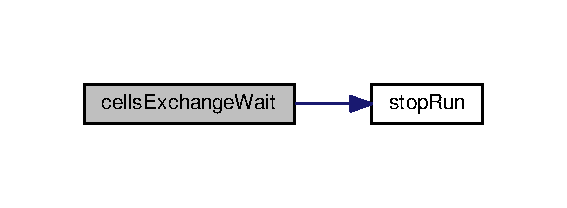
\includegraphics[width=272pt]{comm_8c_ac5b7dbd1157ef088c4e6f8a9f08fcc4b_cgraph}
\end{center}
\end{figure}




Here is the caller graph for this function\-:\nopagebreak
\begin{figure}[H]
\begin{center}
\leavevmode
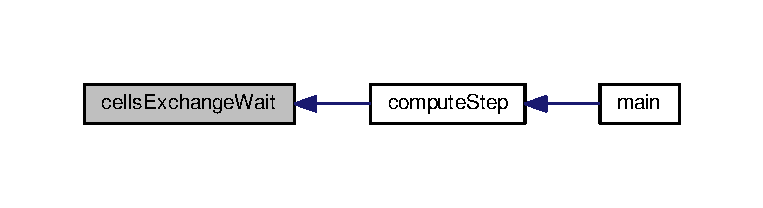
\includegraphics[width=350pt]{comm_8c_ac5b7dbd1157ef088c4e6f8a9f08fcc4b_icgraph}
\end{center}
\end{figure}


\hypertarget{comm_8c_a0a0b21ecf1a24a3cae73074d6bf6c68e}{\index{comm.\-c@{comm.\-c}!comm\-\_\-compare\-\_\-exp\-\_\-list@{comm\-\_\-compare\-\_\-exp\-\_\-list}}
\index{comm\-\_\-compare\-\_\-exp\-\_\-list@{comm\-\_\-compare\-\_\-exp\-\_\-list}!comm.c@{comm.\-c}}
\subsubsection[{comm\-\_\-compare\-\_\-exp\-\_\-list}]{\setlength{\rightskip}{0pt plus 5cm}int comm\-\_\-compare\-\_\-exp\-\_\-list (
\begin{DoxyParamCaption}
\item[{const void $\ast$}]{a, }
\item[{const void $\ast$}]{b}
\end{DoxyParamCaption}
)}}\label{comm_8c_a0a0b21ecf1a24a3cae73074d6bf6c68e}
This function is a comparison function used for sorting export list table. 

Definition at line 54 of file comm.\-c.


\begin{DoxyCode}
55 \{
56   \textcolor{keywordflow}{return} ((\textcolor{keyword}{struct} \hyperlink{structexpData}{expData} *) a)->proc - ((\textcolor{keyword}{struct }\hyperlink{structexpData}{expData} *) \hyperlink{tempf_8c_a74a523afdfebddf9b6b280e545977c5a}{b})->proc;
57 \}
\end{DoxyCode}


Here is the caller graph for this function\-:\nopagebreak
\begin{figure}[H]
\begin{center}
\leavevmode
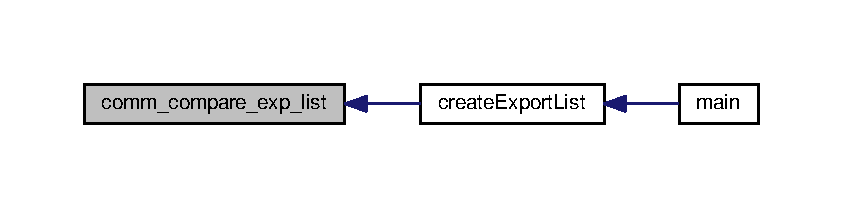
\includegraphics[width=350pt]{comm_8c_a0a0b21ecf1a24a3cae73074d6bf6c68e_icgraph}
\end{center}
\end{figure}


\hypertarget{comm_8c_abdd72f1d40c6c4bf47ad78c4f3c349d5}{\index{comm.\-c@{comm.\-c}!comm\-Cleanup@{comm\-Cleanup}}
\index{comm\-Cleanup@{comm\-Cleanup}!comm.c@{comm.\-c}}
\subsubsection[{comm\-Cleanup}]{\setlength{\rightskip}{0pt plus 5cm}void comm\-Cleanup (
\begin{DoxyParamCaption}
{}
\end{DoxyParamCaption}
)}}\label{comm_8c_abdd72f1d40c6c4bf47ad78c4f3c349d5}
This function deallocates all communication buffers and auxiliary tables. 

Definition at line 156 of file comm.\-c.



References M\-P\-Isize, nc, recv\-Count, recv\-Data, recv\-Dens\-Pot\-Data, recv\-Offset, send\-Count, and send\-Offset.


\begin{DoxyCode}
157 \{
158   \textcolor{keywordflow}{if} (\hyperlink{global_8h_a0845b4b004824f1fe3cd69db1672fa15}{nc} < \hyperlink{global_8h_a0d7d02544d01ceac87c9d5cadc3af0df}{MPIsize} || \hyperlink{global_8h_a0d7d02544d01ceac87c9d5cadc3af0df}{MPIsize} == 1)
159     \textcolor{keywordflow}{return};
160 
161 \textcolor{preprocessor}{#ifdef \_\_MIC\_\_}
162 \textcolor{preprocessor}{}  \_mm\_free(\hyperlink{global_8h_a9909963356d98bc262c21fed8a950cc2}{recvData});
163   \_mm\_free(\hyperlink{global_8h_acf6348786f3c9c222f2ce4894382bcd4}{recvDensPotData});
164 \textcolor{preprocessor}{#else}
165 \textcolor{preprocessor}{}  free(\hyperlink{global_8h_a9909963356d98bc262c21fed8a950cc2}{recvData});
166   free(\hyperlink{global_8h_acf6348786f3c9c222f2ce4894382bcd4}{recvDensPotData});
167 \textcolor{preprocessor}{#endif}
168 \textcolor{preprocessor}{}
169   free(\hyperlink{comm_8c_a6f7e234508139d1113a2f60a1b36c04a}{expList});
170 
171   free(\hyperlink{comm_8c_a073b7079fe649b9ae1b5c4056ccaa4fb}{recvCount});
172   free(\hyperlink{comm_8c_aed19f012b3fe7ae1966dcc8b89cdf7b2}{sendCount});
173 
174   free(\hyperlink{comm_8c_a16d801f1b7f6a598f31107a146b11f16}{sendOffset});
175   free(\hyperlink{comm_8c_a4f0cc30ef1f6185ba3d6406343e1a574}{recvOffset});
176 
177 \}
\end{DoxyCode}


Here is the caller graph for this function\-:\nopagebreak
\begin{figure}[H]
\begin{center}
\leavevmode
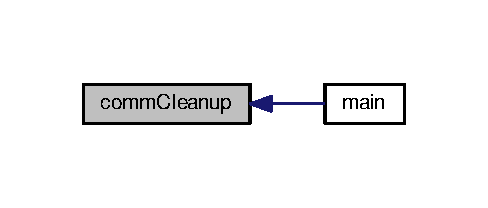
\includegraphics[width=234pt]{comm_8c_abdd72f1d40c6c4bf47ad78c4f3c349d5_icgraph}
\end{center}
\end{figure}


\hypertarget{comm_8c_a191bffd6b8283bf118dec0d0422fa2b3}{\index{comm.\-c@{comm.\-c}!create\-Export\-List@{create\-Export\-List}}
\index{create\-Export\-List@{create\-Export\-List}!comm.c@{comm.\-c}}
\subsubsection[{create\-Export\-List}]{\setlength{\rightskip}{0pt plus 5cm}void create\-Export\-List (
\begin{DoxyParamCaption}
{}
\end{DoxyParamCaption}
)}}\label{comm_8c_a191bffd6b8283bf118dec0d0422fa2b3}
This function uses Zoltan's library function Zoltan\-\_\-\-L\-B\-\_\-\-Box\-\_\-\-Assign to find possible intersections of cells' neighbourhoods and other processes' geometries. 

Definition at line 64 of file comm.\-c.



References exp\-Data\-::cell, cells, comm\-\_\-compare\-\_\-exp\-\_\-list(), h, cell\-Data\-::halo, lnc, M\-A\-X\-\_\-\-E\-X\-P\-O\-R\-T\-E\-D\-\_\-\-P\-E\-R\-\_\-\-P\-R\-O\-C, M\-P\-Irank, M\-P\-Isize, nc, num\-Exp, num\-Imp, exp\-Data\-::proc, recv\-Count, recv\-Offset, sdim, send\-Count, send\-Offset, stop\-Run(), tlnc, cell\-Data\-::x, cell\-Data\-::y, cell\-Data\-::z, and ztn.


\begin{DoxyCode}
65 \{
66 
67   \textcolor{keywordtype}{int} i, p;
68   \textcolor{keywordtype}{int} procs[\hyperlink{global_8h_a0d7d02544d01ceac87c9d5cadc3af0df}{MPIsize}];
69   \textcolor{keywordtype}{int} numprocs;
70 
71   \hyperlink{global_8h_a4c3c9a79704128f7fcc9ebf4bdd9e3fc}{numExp} = 0;
72   \hyperlink{global_8h_a07792d8e2788e030124304f47e8cf1f6}{numImp} = 0;
73   \textcolor{keywordflow}{if} (\hyperlink{global_8h_a0845b4b004824f1fe3cd69db1672fa15}{nc} < \hyperlink{global_8h_a0d7d02544d01ceac87c9d5cadc3af0df}{MPIsize} || \hyperlink{global_8h_a0d7d02544d01ceac87c9d5cadc3af0df}{MPIsize} == 1)
74     \textcolor{keywordflow}{return};
75 
76   \hyperlink{comm_8c_a6f7e234508139d1113a2f60a1b36c04a}{expList} =
77     (\textcolor{keyword}{struct }\hyperlink{structexpData}{expData} *) malloc(\textcolor{keyword}{sizeof}(\textcolor{keyword}{struct} \hyperlink{structexpData}{expData}) *
78                               \hyperlink{comm_8c_a93da5acfae81b763e797f8562d49ca64}{MAX\_EXPORTED\_PER\_PROC});
79   \hyperlink{comm_8c_a073b7079fe649b9ae1b5c4056ccaa4fb}{recvCount} = (\textcolor{keywordtype}{int} *) calloc(\hyperlink{global_8h_a0d7d02544d01ceac87c9d5cadc3af0df}{MPIsize}, \textcolor{keyword}{sizeof}(\textcolor{keywordtype}{int}));
80   \hyperlink{comm_8c_aed19f012b3fe7ae1966dcc8b89cdf7b2}{sendCount} = (\textcolor{keywordtype}{int} *) calloc(\hyperlink{global_8h_a0d7d02544d01ceac87c9d5cadc3af0df}{MPIsize}, \textcolor{keyword}{sizeof}(\textcolor{keywordtype}{int}));
81   \hyperlink{comm_8c_a16d801f1b7f6a598f31107a146b11f16}{sendOffset} = (int64\_t *) calloc(\hyperlink{global_8h_a0d7d02544d01ceac87c9d5cadc3af0df}{MPIsize}, \textcolor{keyword}{sizeof}(int64\_t));
82   \hyperlink{comm_8c_a4f0cc30ef1f6185ba3d6406343e1a574}{recvOffset} = (int64\_t *) calloc(\hyperlink{global_8h_a0d7d02544d01ceac87c9d5cadc3af0df}{MPIsize}, \textcolor{keyword}{sizeof}(int64\_t));
83 
84   \textcolor{comment}{/* loop over local cells */}
85   \textcolor{comment}{/*#pragma omp parallel for private(procs) */}
86   \textcolor{keywordflow}{for} (p = 0; p < \hyperlink{global_8h_a7065c019590815f10169c219f358e7d0}{lnc}; p++) \{
87     \textcolor{keywordtype}{double} xmin, xmax, ymin, ymax, zmin, zmax;
88     \textcolor{keywordtype}{double} r;
89 
90     \hyperlink{global_8h_a3ea537bde8d64e54770a2bd81e3f00be}{cells}[p].\hyperlink{structcellData_a80ff3fcc4d03d0b1b01559839d12df5b}{halo} = 0;
91 
92     \textcolor{keywordflow}{if} (\hyperlink{global_8h_a0845b4b004824f1fe3cd69db1672fa15}{nc} < \hyperlink{global_8h_a0d7d02544d01ceac87c9d5cadc3af0df}{MPIsize})
93       \textcolor{keywordflow}{continue};
94 
95     r = \hyperlink{global_8h_adae58efd3b7d9072a77aff9c63040d05}{h} * 1.5;
96 
97     \textcolor{comment}{/* compute neighbourhood box */}
98     xmin = \hyperlink{global_8h_a3ea537bde8d64e54770a2bd81e3f00be}{cells}[p].\hyperlink{structcellData_af88b946fb90d5f08b5fb740c70e98c10}{x} - r;
99     xmax = \hyperlink{global_8h_a3ea537bde8d64e54770a2bd81e3f00be}{cells}[p].\hyperlink{structcellData_af88b946fb90d5f08b5fb740c70e98c10}{x} + r;
100     ymin = \hyperlink{global_8h_a3ea537bde8d64e54770a2bd81e3f00be}{cells}[p].\hyperlink{structcellData_ab927965981178aa1fba979a37168db2a}{y} - r;
101     ymax = \hyperlink{global_8h_a3ea537bde8d64e54770a2bd81e3f00be}{cells}[p].\hyperlink{structcellData_ab927965981178aa1fba979a37168db2a}{y} + r;
102     \textcolor{keywordflow}{if} (\hyperlink{global_8h_a9fad6472ef73b07a138721c11022697a}{sdim} == 3) \{
103       zmin = \hyperlink{global_8h_a3ea537bde8d64e54770a2bd81e3f00be}{cells}[p].\hyperlink{structcellData_ab3e6ed577a7c669c19de1f9c1b46c872}{z} - r;
104       zmax = \hyperlink{global_8h_a3ea537bde8d64e54770a2bd81e3f00be}{cells}[p].\hyperlink{structcellData_ab3e6ed577a7c669c19de1f9c1b46c872}{z} + r;
105     \} \textcolor{keywordflow}{else} \{
106       zmin = 0.0;
107       zmax = 0.0;
108     \}
109 
110     \textcolor{comment}{/* look for possible neighbours */}
111     Zoltan\_LB\_Box\_Assign(\hyperlink{global_8h_afc06c50b11f3b60d3738e669b612eb9c}{ztn}, xmin, ymin, zmin, xmax, ymax, zmax, procs,
112                          &numprocs);
113 
114     \textcolor{comment}{/* loop over receivers */}
115     \textcolor{keywordflow}{for} (i = 0; i < numprocs; i++) \{
116       \textcolor{keywordflow}{if} (procs[i] == \hyperlink{global_8h_a710288ab7d2734acc4566a87a645325d}{MPIrank} || \hyperlink{global_8h_ac3c96b975a3376c555ad22a7d2688b2f}{tlnc}[procs[i]] == 0)
117         \textcolor{keywordflow}{continue};
118       \hyperlink{comm_8c_a6f7e234508139d1113a2f60a1b36c04a}{expList}[\hyperlink{global_8h_a4c3c9a79704128f7fcc9ebf4bdd9e3fc}{numExp}].\hyperlink{structexpData_af00601a22186810a9e6d16efb75862ce}{cell} = p;
119       \hyperlink{comm_8c_a6f7e234508139d1113a2f60a1b36c04a}{expList}[\hyperlink{global_8h_a4c3c9a79704128f7fcc9ebf4bdd9e3fc}{numExp}].\hyperlink{structexpData_a7e9d757c9982bd721d598bad366fbe62}{proc} = procs[i];
120       \hyperlink{global_8h_a3ea537bde8d64e54770a2bd81e3f00be}{cells}[p].\hyperlink{structcellData_a80ff3fcc4d03d0b1b01559839d12df5b}{halo} = \hyperlink{global_8h_a710288ab7d2734acc4566a87a645325d}{MPIrank} + 1;
121       \hyperlink{comm_8c_aed19f012b3fe7ae1966dcc8b89cdf7b2}{sendCount}[procs[i]]++;
122       \hyperlink{global_8h_a4c3c9a79704128f7fcc9ebf4bdd9e3fc}{numExp}++;
123       \textcolor{comment}{/* upps! too many refugees */}
124       \textcolor{keywordflow}{if} (\hyperlink{global_8h_a4c3c9a79704128f7fcc9ebf4bdd9e3fc}{numExp} >= \hyperlink{comm_8c_a93da5acfae81b763e797f8562d49ca64}{MAX\_EXPORTED\_PER\_PROC})
125         \hyperlink{utils_8c_a07dd99a04f2723be164531a7a862fb67}{stopRun}(110, NULL, \_\_FILE\_\_, \_\_LINE\_\_);
126     \}
127   \}
128 
129   \textcolor{comment}{/* sort export list with respect to process number */}
130   qsort(\hyperlink{comm_8c_a6f7e234508139d1113a2f60a1b36c04a}{expList}, \hyperlink{global_8h_a4c3c9a79704128f7fcc9ebf4bdd9e3fc}{numExp}, \textcolor{keyword}{sizeof}(\textcolor{keyword}{struct} \hyperlink{structexpData}{expData}), 
      \hyperlink{comm_8c_a0a0b21ecf1a24a3cae73074d6bf6c68e}{comm\_compare\_exp\_list});
131 
132   \textcolor{comment}{/* distribute the information on transfer sizes between each process */}
133   MPI\_Alltoall(\hyperlink{comm_8c_aed19f012b3fe7ae1966dcc8b89cdf7b2}{sendCount}, 1, MPI\_INT, \hyperlink{comm_8c_a073b7079fe649b9ae1b5c4056ccaa4fb}{recvCount}, 1, MPI\_INT,
134                MPI\_COMM\_WORLD);
135 
136   \textcolor{comment}{/* compute send offsets */}
137   \hyperlink{comm_8c_a16d801f1b7f6a598f31107a146b11f16}{sendOffset}[0] = 0;
138   \textcolor{keywordflow}{for} (i = 1; i < \hyperlink{global_8h_a0d7d02544d01ceac87c9d5cadc3af0df}{MPIsize}; i++)
139     \hyperlink{comm_8c_a16d801f1b7f6a598f31107a146b11f16}{sendOffset}[i] = \hyperlink{comm_8c_a16d801f1b7f6a598f31107a146b11f16}{sendOffset}[i - 1] + \hyperlink{comm_8c_aed19f012b3fe7ae1966dcc8b89cdf7b2}{sendCount}[i - 1];
140 
141   \textcolor{comment}{/* compute receive offsets */}
142   \hyperlink{comm_8c_a4f0cc30ef1f6185ba3d6406343e1a574}{recvOffset}[0] = 0;
143   \textcolor{keywordflow}{for} (i = 1; i < \hyperlink{global_8h_a0d7d02544d01ceac87c9d5cadc3af0df}{MPIsize}; i++)
144     \hyperlink{comm_8c_a4f0cc30ef1f6185ba3d6406343e1a574}{recvOffset}[i] = \hyperlink{comm_8c_a4f0cc30ef1f6185ba3d6406343e1a574}{recvOffset}[i - 1] + \hyperlink{comm_8c_a073b7079fe649b9ae1b5c4056ccaa4fb}{recvCount}[i - 1];
145 
146   \textcolor{comment}{/* count cells to be imported */}
147   \textcolor{keywordflow}{for} (i = 0; i < \hyperlink{global_8h_a0d7d02544d01ceac87c9d5cadc3af0df}{MPIsize}; i++)
148     \hyperlink{global_8h_a07792d8e2788e030124304f47e8cf1f6}{numImp} += \hyperlink{comm_8c_a073b7079fe649b9ae1b5c4056ccaa4fb}{recvCount}[i];
149 
150 \}
\end{DoxyCode}


Here is the call graph for this function\-:\nopagebreak
\begin{figure}[H]
\begin{center}
\leavevmode
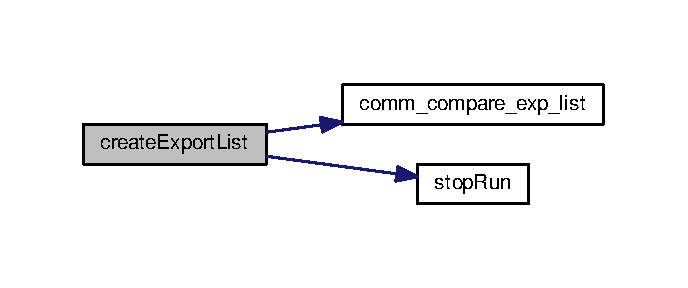
\includegraphics[width=330pt]{comm_8c_a191bffd6b8283bf118dec0d0422fa2b3_cgraph}
\end{center}
\end{figure}




Here is the caller graph for this function\-:\nopagebreak
\begin{figure}[H]
\begin{center}
\leavevmode
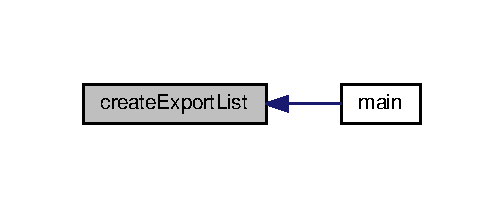
\includegraphics[width=242pt]{comm_8c_a191bffd6b8283bf118dec0d0422fa2b3_icgraph}
\end{center}
\end{figure}


\hypertarget{comm_8c_a206e073b7e35f281184b3487b3bbc055}{\index{comm.\-c@{comm.\-c}!dens\-Pot\-Exchange\-Init@{dens\-Pot\-Exchange\-Init}}
\index{dens\-Pot\-Exchange\-Init@{dens\-Pot\-Exchange\-Init}!comm.c@{comm.\-c}}
\subsubsection[{dens\-Pot\-Exchange\-Init}]{\setlength{\rightskip}{0pt plus 5cm}void dens\-Pot\-Exchange\-Init (
\begin{DoxyParamCaption}
{}
\end{DoxyParamCaption}
)}}\label{comm_8c_a206e073b7e35f281184b3487b3bbc055}
This function initiate sending and receiving density and potential values between processes. 

Definition at line 267 of file comm.\-c.



References exp\-Data\-::cell, cells, cell\-Data\-::density, dens\-Pot\-Data\-::density, lnc, M\-P\-Irank, M\-P\-Isize, nc, num\-Exp, num\-Imp, recv\-Count, recv\-Dens\-Pot\-Data, recv\-Offset, req\-Recv, req\-Send, send\-Count, send\-Dens\-Pot\-Data, send\-Offset, tlnc, cell\-Data\-::v, and dens\-Pot\-Data\-::v.


\begin{DoxyCode}
268 \{
269   \textcolor{keywordtype}{int} i;
270 
271   \textcolor{keywordflow}{if} (\hyperlink{global_8h_a0845b4b004824f1fe3cd69db1672fa15}{nc} < \hyperlink{global_8h_a0d7d02544d01ceac87c9d5cadc3af0df}{MPIsize} || \hyperlink{global_8h_a0d7d02544d01ceac87c9d5cadc3af0df}{MPIsize} == 1)
272     \textcolor{keywordflow}{return};
273 
274   \textcolor{comment}{/* allocate communication buffers */}
275   \hyperlink{global_8h_a5b0d78dc19924c0af131438356bfcdbd}{sendDensPotData} =
276     (\textcolor{keyword}{struct }\hyperlink{structdensPotData}{densPotData} *) malloc(\hyperlink{global_8h_a4c3c9a79704128f7fcc9ebf4bdd9e3fc}{numExp} * \textcolor{keyword}{sizeof}(\textcolor{keyword}{struct} 
      \hyperlink{structdensPotData}{densPotData}));
277 \textcolor{preprocessor}{#ifdef \_\_MIC\_\_}
278 \textcolor{preprocessor}{}  \hyperlink{global_8h_acf6348786f3c9c222f2ce4894382bcd4}{recvDensPotData} =
279     (\textcolor{keyword}{struct }\hyperlink{structdensPotData}{densPotData} *) \_mm\_malloc(\hyperlink{global_8h_a07792d8e2788e030124304f47e8cf1f6}{numImp} * \textcolor{keyword}{sizeof}(\textcolor{keyword}{struct} 
      \hyperlink{structdensPotData}{densPotData}),64);
280 \textcolor{preprocessor}{#else}
281 \textcolor{preprocessor}{}  \hyperlink{global_8h_acf6348786f3c9c222f2ce4894382bcd4}{recvDensPotData} =
282     (\textcolor{keyword}{struct }\hyperlink{structdensPotData}{densPotData} *) malloc(\hyperlink{global_8h_a07792d8e2788e030124304f47e8cf1f6}{numImp} * \textcolor{keyword}{sizeof}(\textcolor{keyword}{struct} 
      \hyperlink{structdensPotData}{densPotData}));
283 \textcolor{preprocessor}{#endif}
284 \textcolor{preprocessor}{}  \hyperlink{comm_8c_a827e028e778c94dd2e816ae6077a3198}{reqSend} = (MPI\_Request *) malloc(\textcolor{keyword}{sizeof}(MPI\_Request) * \hyperlink{global_8h_a0d7d02544d01ceac87c9d5cadc3af0df}{MPIsize});
285   \hyperlink{comm_8c_ad7a9f44424272a25979b199886bdce73}{reqRecv} = (MPI\_Request *) malloc(\textcolor{keyword}{sizeof}(MPI\_Request) * \hyperlink{global_8h_a0d7d02544d01ceac87c9d5cadc3af0df}{MPIsize});
286 
287   \textcolor{comment}{/* create density and potential buffer for exporting */}
288   \textcolor{keywordflow}{for} (i = 0; i < \hyperlink{global_8h_a4c3c9a79704128f7fcc9ebf4bdd9e3fc}{numExp}; i++) \{
289     \hyperlink{global_8h_a5b0d78dc19924c0af131438356bfcdbd}{sendDensPotData}[i].\hyperlink{structdensPotData_a3b90d5a73541ab9402511d87bed076ef}{v} = \hyperlink{global_8h_a3ea537bde8d64e54770a2bd81e3f00be}{cells}[\hyperlink{comm_8c_a6f7e234508139d1113a2f60a1b36c04a}{expList}[i].\hyperlink{structexpData_af00601a22186810a9e6d16efb75862ce}{cell}].
      \hyperlink{structcellData_a3b90d5a73541ab9402511d87bed076ef}{v};
290     \hyperlink{global_8h_a5b0d78dc19924c0af131438356bfcdbd}{sendDensPotData}[i].\hyperlink{structdensPotData_a6f8c052f8417728038991f7f2826d38d}{density} = \hyperlink{global_8h_a3ea537bde8d64e54770a2bd81e3f00be}{cells}[\hyperlink{comm_8c_a6f7e234508139d1113a2f60a1b36c04a}{expList}[i].
      \hyperlink{structexpData_af00601a22186810a9e6d16efb75862ce}{cell}].\hyperlink{structcellData_a6f8c052f8417728038991f7f2826d38d}{density};
291   \}
292 
293   \textcolor{comment}{/* send data - asynchronous MPI call */}
294   \textcolor{keywordflow}{for} (i = 0; i < \hyperlink{global_8h_a0d7d02544d01ceac87c9d5cadc3af0df}{MPIsize}; i++) \{
295     \textcolor{keywordflow}{if} (\hyperlink{comm_8c_aed19f012b3fe7ae1966dcc8b89cdf7b2}{sendCount}[i] == 0 || \hyperlink{global_8h_ac3c96b975a3376c555ad22a7d2688b2f}{tlnc}[i] == 0 || \hyperlink{global_8h_a7065c019590815f10169c219f358e7d0}{lnc} == 0)
296       \textcolor{keywordflow}{continue};
297     MPI\_Isend(&\hyperlink{global_8h_a5b0d78dc19924c0af131438356bfcdbd}{sendDensPotData}[\hyperlink{comm_8c_a16d801f1b7f6a598f31107a146b11f16}{sendOffset}[i]],
298               \hyperlink{comm_8c_aed19f012b3fe7ae1966dcc8b89cdf7b2}{sendCount}[i] * \textcolor{keyword}{sizeof}(\textcolor{keyword}{struct} \hyperlink{structdensPotData}{densPotData}), MPI\_BYTE, i,
299               \hyperlink{global_8h_a710288ab7d2734acc4566a87a645325d}{MPIrank}, MPI\_COMM\_WORLD, &\hyperlink{comm_8c_a827e028e778c94dd2e816ae6077a3198}{reqSend}[i]);
300   \}
301 
302   \textcolor{comment}{/* receive data - asynchronous MPI call */}
303   \textcolor{keywordflow}{for} (i = 0; i < \hyperlink{global_8h_a0d7d02544d01ceac87c9d5cadc3af0df}{MPIsize}; i++) \{
304     \textcolor{keywordflow}{if} (\hyperlink{comm_8c_a073b7079fe649b9ae1b5c4056ccaa4fb}{recvCount}[i] == 0 || \hyperlink{global_8h_ac3c96b975a3376c555ad22a7d2688b2f}{tlnc}[i] == 0 || \hyperlink{global_8h_a7065c019590815f10169c219f358e7d0}{lnc} == 0)
305       \textcolor{keywordflow}{continue};
306     MPI\_Irecv(&\hyperlink{global_8h_acf6348786f3c9c222f2ce4894382bcd4}{recvDensPotData}[\hyperlink{comm_8c_a4f0cc30ef1f6185ba3d6406343e1a574}{recvOffset}[i]],
307               \hyperlink{comm_8c_a073b7079fe649b9ae1b5c4056ccaa4fb}{recvCount}[i] * \textcolor{keyword}{sizeof}(\textcolor{keyword}{struct} \hyperlink{structdensPotData}{densPotData}), MPI\_BYTE, i, i,
308               MPI\_COMM\_WORLD, &\hyperlink{comm_8c_ad7a9f44424272a25979b199886bdce73}{reqRecv}[i]);
309   \}
310 
311 \}
\end{DoxyCode}


Here is the caller graph for this function\-:\nopagebreak
\begin{figure}[H]
\begin{center}
\leavevmode
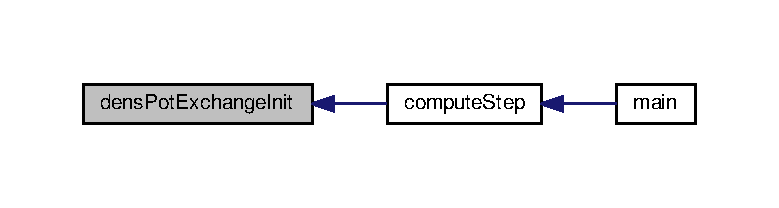
\includegraphics[width=350pt]{comm_8c_a206e073b7e35f281184b3487b3bbc055_icgraph}
\end{center}
\end{figure}


\hypertarget{comm_8c_afebf59220f4170178e5fb828d569aaab}{\index{comm.\-c@{comm.\-c}!dens\-Pot\-Exchange\-Wait@{dens\-Pot\-Exchange\-Wait}}
\index{dens\-Pot\-Exchange\-Wait@{dens\-Pot\-Exchange\-Wait}!comm.c@{comm.\-c}}
\subsubsection[{dens\-Pot\-Exchange\-Wait}]{\setlength{\rightskip}{0pt plus 5cm}void dens\-Pot\-Exchange\-Wait (
\begin{DoxyParamCaption}
{}
\end{DoxyParamCaption}
)}}\label{comm_8c_afebf59220f4170178e5fb828d569aaab}
This function waits for density and potential data exchange completion. 

Definition at line 316 of file comm.\-c.



References lnc, M\-P\-Isize, nc, recv\-Count, req\-Recv, req\-Send, send\-Count, send\-Dens\-Pot\-Data, stop\-Run(), and tlnc.


\begin{DoxyCode}
317 \{
318   \textcolor{keywordtype}{int} i;
319   MPI\_Status status;
320 
321   \textcolor{keywordflow}{if} (\hyperlink{global_8h_a0845b4b004824f1fe3cd69db1672fa15}{nc} < \hyperlink{global_8h_a0d7d02544d01ceac87c9d5cadc3af0df}{MPIsize} || \hyperlink{global_8h_a0d7d02544d01ceac87c9d5cadc3af0df}{MPIsize} == 1)
322     \textcolor{keywordflow}{return};
323 
324   \textcolor{comment}{// Wait for send completion}
325   \textcolor{keywordflow}{for} (i = 0; i < \hyperlink{global_8h_a0d7d02544d01ceac87c9d5cadc3af0df}{MPIsize}; i++) \{
326     \textcolor{keywordflow}{if} (\hyperlink{comm_8c_aed19f012b3fe7ae1966dcc8b89cdf7b2}{sendCount}[i] == 0 || \hyperlink{global_8h_ac3c96b975a3376c555ad22a7d2688b2f}{tlnc}[i] == 0 || \hyperlink{global_8h_a7065c019590815f10169c219f358e7d0}{lnc} == 0)
327       \textcolor{keywordflow}{continue};
328     \textcolor{keywordflow}{if} (MPI\_Wait(&\hyperlink{comm_8c_a827e028e778c94dd2e816ae6077a3198}{reqSend}[i], &status) != MPI\_SUCCESS)
329       \hyperlink{utils_8c_a07dd99a04f2723be164531a7a862fb67}{stopRun}(103, \textcolor{stringliteral}{"sending"}, \_\_FILE\_\_, \_\_LINE\_\_);
330   \}
331 
332   \textcolor{comment}{// Wait for receive completion}
333   \textcolor{keywordflow}{for} (i = 0; i < \hyperlink{global_8h_a0d7d02544d01ceac87c9d5cadc3af0df}{MPIsize}; i++) \{
334     \textcolor{keywordflow}{if} (\hyperlink{comm_8c_a073b7079fe649b9ae1b5c4056ccaa4fb}{recvCount}[i] == 0 || \hyperlink{global_8h_ac3c96b975a3376c555ad22a7d2688b2f}{tlnc}[i] == 0 || \hyperlink{global_8h_a7065c019590815f10169c219f358e7d0}{lnc} == 0)
335       \textcolor{keywordflow}{continue};
336     \textcolor{keywordflow}{if} (MPI\_Wait(&\hyperlink{comm_8c_ad7a9f44424272a25979b199886bdce73}{reqRecv}[i], &status) != MPI\_SUCCESS)
337       \hyperlink{utils_8c_a07dd99a04f2723be164531a7a862fb67}{stopRun}(103, \textcolor{stringliteral}{"receiving"}, \_\_FILE\_\_, \_\_LINE\_\_);
338   \}
339 
340   \textcolor{comment}{/* some of the buffers can be deallocated */}
341   free(\hyperlink{global_8h_a5b0d78dc19924c0af131438356bfcdbd}{sendDensPotData});
342   free(\hyperlink{comm_8c_a827e028e778c94dd2e816ae6077a3198}{reqSend});
343   free(\hyperlink{comm_8c_ad7a9f44424272a25979b199886bdce73}{reqRecv});
344 \}
\end{DoxyCode}


Here is the call graph for this function\-:\nopagebreak
\begin{figure}[H]
\begin{center}
\leavevmode
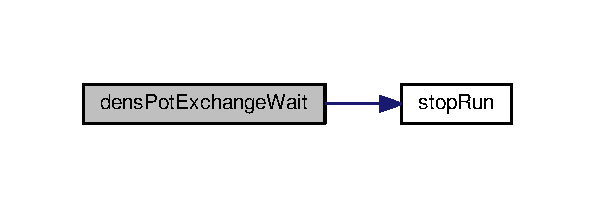
\includegraphics[width=286pt]{comm_8c_afebf59220f4170178e5fb828d569aaab_cgraph}
\end{center}
\end{figure}




Here is the caller graph for this function\-:\nopagebreak
\begin{figure}[H]
\begin{center}
\leavevmode
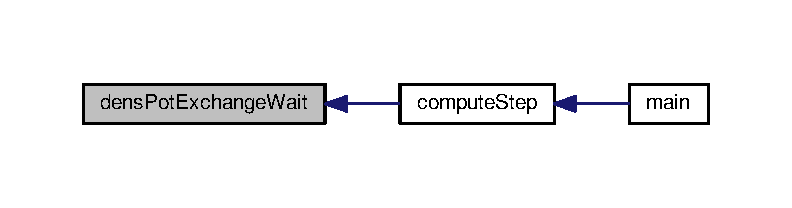
\includegraphics[width=350pt]{comm_8c_afebf59220f4170178e5fb828d569aaab_icgraph}
\end{center}
\end{figure}




\subsection{Variable Documentation}
\hypertarget{comm_8c_a6f7e234508139d1113a2f60a1b36c04a}{\index{comm.\-c@{comm.\-c}!exp\-List@{exp\-List}}
\index{exp\-List@{exp\-List}!comm.c@{comm.\-c}}
\subsubsection[{exp\-List}]{\setlength{\rightskip}{0pt plus 5cm}struct {\bf exp\-Data}$\ast$ exp\-List}}\label{comm_8c_a6f7e234508139d1113a2f60a1b36c04a}


Definition at line 43 of file comm.\-c.

\hypertarget{comm_8c_a073b7079fe649b9ae1b5c4056ccaa4fb}{\index{comm.\-c@{comm.\-c}!recv\-Count@{recv\-Count}}
\index{recv\-Count@{recv\-Count}!comm.c@{comm.\-c}}
\subsubsection[{recv\-Count}]{\setlength{\rightskip}{0pt plus 5cm}int$\ast$ recv\-Count}}\label{comm_8c_a073b7079fe649b9ae1b5c4056ccaa4fb}


Definition at line 45 of file comm.\-c.

\hypertarget{comm_8c_a4f0cc30ef1f6185ba3d6406343e1a574}{\index{comm.\-c@{comm.\-c}!recv\-Offset@{recv\-Offset}}
\index{recv\-Offset@{recv\-Offset}!comm.c@{comm.\-c}}
\subsubsection[{recv\-Offset}]{\setlength{\rightskip}{0pt plus 5cm}int64\-\_\-t$\ast$ recv\-Offset}}\label{comm_8c_a4f0cc30ef1f6185ba3d6406343e1a574}


Definition at line 41 of file comm.\-c.

\hypertarget{comm_8c_ad7a9f44424272a25979b199886bdce73}{\index{comm.\-c@{comm.\-c}!req\-Recv@{req\-Recv}}
\index{req\-Recv@{req\-Recv}!comm.c@{comm.\-c}}
\subsubsection[{req\-Recv}]{\setlength{\rightskip}{0pt plus 5cm}M\-P\-I\-\_\-\-Request$\ast$ req\-Recv}}\label{comm_8c_ad7a9f44424272a25979b199886bdce73}


Definition at line 38 of file comm.\-c.

\hypertarget{comm_8c_a827e028e778c94dd2e816ae6077a3198}{\index{comm.\-c@{comm.\-c}!req\-Send@{req\-Send}}
\index{req\-Send@{req\-Send}!comm.c@{comm.\-c}}
\subsubsection[{req\-Send}]{\setlength{\rightskip}{0pt plus 5cm}M\-P\-I\-\_\-\-Request$\ast$ req\-Send}}\label{comm_8c_a827e028e778c94dd2e816ae6077a3198}


Definition at line 37 of file comm.\-c.

\hypertarget{comm_8c_aed19f012b3fe7ae1966dcc8b89cdf7b2}{\index{comm.\-c@{comm.\-c}!send\-Count@{send\-Count}}
\index{send\-Count@{send\-Count}!comm.c@{comm.\-c}}
\subsubsection[{send\-Count}]{\setlength{\rightskip}{0pt plus 5cm}int$\ast$ send\-Count}}\label{comm_8c_aed19f012b3fe7ae1966dcc8b89cdf7b2}


Definition at line 46 of file comm.\-c.

\hypertarget{comm_8c_a16d801f1b7f6a598f31107a146b11f16}{\index{comm.\-c@{comm.\-c}!send\-Offset@{send\-Offset}}
\index{send\-Offset@{send\-Offset}!comm.c@{comm.\-c}}
\subsubsection[{send\-Offset}]{\setlength{\rightskip}{0pt plus 5cm}int64\-\_\-t$\ast$ send\-Offset}}\label{comm_8c_a16d801f1b7f6a598f31107a146b11f16}


Definition at line 40 of file comm.\-c.


\hypertarget{compute_8c}{\section{compute.\-c File Reference}
\label{compute_8c}\index{compute.\-c@{compute.\-c}}
}


contains main computational function called in each time step of the simulation  


{\ttfamily \#include $<$stdio.\-h$>$}\\*
{\ttfamily \#include $<$stdlib.\-h$>$}\\*
{\ttfamily \#include $<$float.\-h$>$}\\*
{\ttfamily \#include $<$math.\-h$>$}\\*
{\ttfamily \#include \char`\"{}global.\-h\char`\"{}}\\*
{\ttfamily \#include \char`\"{}potential.\-h\char`\"{}}\\*
{\ttfamily \#include \char`\"{}fields.\-h\char`\"{}}\\*
{\ttfamily \#include \char`\"{}inline.\-h\char`\"{}}\\*
Include dependency graph for compute.\-c\-:\nopagebreak
\begin{figure}[H]
\begin{center}
\leavevmode
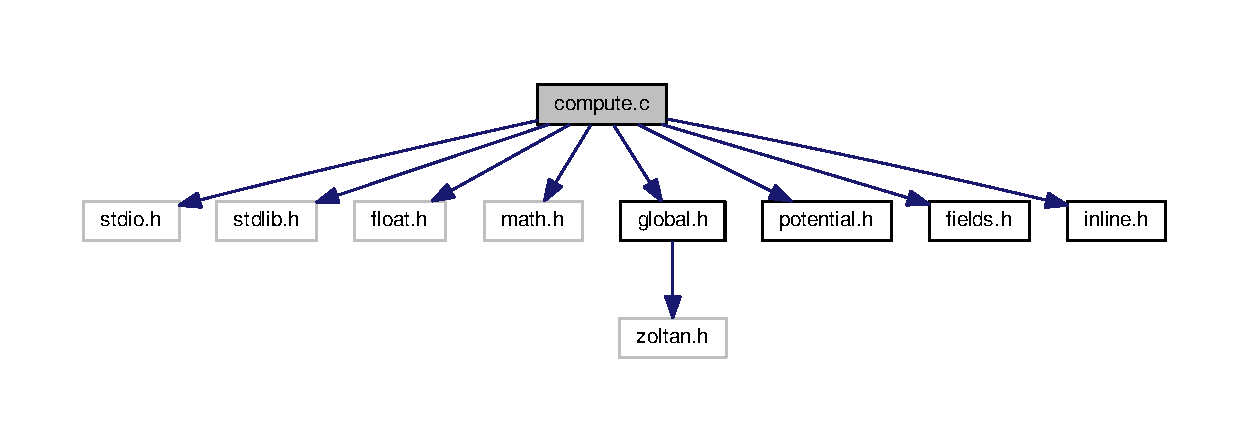
\includegraphics[width=350pt]{compute_8c__incl}
\end{center}
\end{figure}
\subsection*{Functions}
\begin{DoxyCompactItemize}
\item 
int \hyperlink{compute_8c_ae9a79d8510c24a987ad95d908ad4eb50}{compute\-Step} ()
\end{DoxyCompactItemize}


\subsection{Detailed Description}
contains main computational function called in each time step of the simulation 

Definition in file \hyperlink{compute_8c_source}{compute.\-c}.



\subsection{Function Documentation}
\hypertarget{compute_8c_ae9a79d8510c24a987ad95d908ad4eb50}{\index{compute.\-c@{compute.\-c}!compute\-Step@{compute\-Step}}
\index{compute\-Step@{compute\-Step}!compute.c@{compute.\-c}}
\subsubsection[{compute\-Step}]{\setlength{\rightskip}{0pt plus 5cm}int compute\-Step (
\begin{DoxyParamCaption}
{}
\end{DoxyParamCaption}
)}}\label{compute_8c_ae9a79d8510c24a987ad95d908ad4eb50}
This function calls all important simulation steps (cellular dynamics and global fields computations). 

Definition at line 40 of file compute.\-c.



References bvsim, cell\-Fields, cells, cells\-Exchange\-Init(), cells\-Exchange\-Wait(), comp\-Pot(), comp\-Pot\-Grad(), comp\-R\-Pot(), comp\-R\-Pot\-Grad(), dens\-Pot\-Exchange\-Init(), dens\-Pot\-Exchange\-Wait(), field\-Gradient(), fields\-Solve(), global\-Max\-Vel, global\-Min\-Vel, init\-Cells\-To\-Grid\-Exchange(), interpolate\-Fields\-To\-Cells(), lnc, statistics\-Data\-::maxsize, max\-Speed\-In\-Units, statistics\-Data\-::maxvel, statistics\-Data\-::mindist, statistics\-Data\-::minsize, statistics\-Data\-::minvel, nc, N\-F\-I\-E\-L\-D\-S, seconds\-Per\-Step, cell\-Data\-::size, statistics, step, v, velocity, wait\-Cells\-To\-Grid\-Exchange(), x, double\-Vector3d\-::x, double\-Vector3d\-::y, and double\-Vector3d\-::z.


\begin{DoxyCode}
41 \{
42   \textcolor{keywordtype}{int} p;
43   \textcolor{keywordtype}{double} dvel,sf;
44 \textcolor{preprocessor}{#ifdef \_\_MIC\_\_}
45 \textcolor{preprocessor}{}  \textcolor{keywordtype}{double} *phiwork1,*phiwork2;
46 \textcolor{preprocessor}{#endif}
47 \textcolor{preprocessor}{}
48   \textcolor{comment}{/* 0. Initialization */}
49 
50   \textcolor{comment}{/* initialize statistics data */}
51   \textcolor{keywordflow}{if}(\hyperlink{global_8h_a0845b4b004824f1fe3cd69db1672fa15}{nc}>1)
52     \hyperlink{global_8h_aa28392f90ce59a6b79b9b939fd364a9a}{statistics}.\hyperlink{structstatisticsData_a78455d23ec97258967b76cbb2332b7be}{mindist}=DBL\_MAX;
53   \textcolor{keywordflow}{else}
54     \hyperlink{global_8h_aa28392f90ce59a6b79b9b939fd364a9a}{statistics}.\hyperlink{structstatisticsData_a78455d23ec97258967b76cbb2332b7be}{mindist}=0.0;
55   \hyperlink{global_8h_aa28392f90ce59a6b79b9b939fd364a9a}{statistics}.\hyperlink{structstatisticsData_a1b9d00ac67b4ceca8e7747a50edc802b}{minvel}=DBL\_MAX;
56   \hyperlink{global_8h_aa28392f90ce59a6b79b9b939fd364a9a}{statistics}.\hyperlink{structstatisticsData_a485292d20f5d14bd18e83fef65976fb4}{maxvel}=0.0;
57   \hyperlink{global_8h_aa28392f90ce59a6b79b9b939fd364a9a}{statistics}.\hyperlink{structstatisticsData_ad99dc4104d1898b6e593bbf331e41c69}{minsize}=DBL\_MAX;
58   \hyperlink{global_8h_aa28392f90ce59a6b79b9b939fd364a9a}{statistics}.\hyperlink{structstatisticsData_a7383c898fd4cd4d862ca65d3713086cd}{maxsize}=0.0;
59 
60   \hyperlink{interp_8c_ad862fb7e08b1dee6d784a09a26978ada}{initCellsToGridExchange}();
61 
62   \textcolor{comment}{/* initiate asynchronous data transfers between processors */}
63   \hyperlink{comm_8c_aa92fc6732720bc9accbbdef7fb02384f}{cellsExchangeInit}();
64 
65   \textcolor{comment}{/* 1. Compute potential for local cells */}
66 
67   \textcolor{comment}{/* offload trasfer: host -> accelerator  */}
68 \textcolor{preprocessor}{#ifdef \_\_MIC\_\_}
69 \textcolor{preprocessor}{}\textcolor{preprocessor}{#pragma offload\_transfer target(mic:MPIrank%2) in(cells:length(lnc) alloc\_if(1) free\_if(0))
       in(octree:length(octSize) alloc\_if(1) free\_if(0)) nocopy(velocity:length(lnc) alloc\_if(1) free\_if(0)) in(statistics)}
70 \textcolor{preprocessor}{}\textcolor{preprocessor}{#endif}
71 \textcolor{preprocessor}{}  \textcolor{comment}{/* compute potential for local cells */}
72 \textcolor{preprocessor}{#ifdef \_\_MIC\_\_}
73 \textcolor{preprocessor}{}\textcolor{preprocessor}{#pragma offload target(mic:MPIrank%2) signal(phiwork1) nocopy(cells:length(lnc) alloc\_if(0) free\_if(0))
       nocopy(octree:length(octSize) alloc\_if(0) free\_if(0)) in(affShift,affScale,h,tnc,lnc,nx,sdim,h2,h3,csize)}
74 \textcolor{preprocessor}{}\textcolor{preprocessor}{#endif}
75 \textcolor{preprocessor}{}  \hyperlink{potential_8c_ac7aa3d6bad50d0aeec842c955c0a6fbc}{compPot}();
76 
77   \textcolor{comment}{/* 2. Solve global fields */}
78 
79   \textcolor{keywordflow}{if}(\hyperlink{global_8h_abc16e65f240ed0c8f3e876e8732c0a33}{step}>0) \{
80     \hyperlink{interp_8c_ac7fd669461f281bbaceac377028fb722}{waitCellsToGridExchange}();
81     \hyperlink{fields_8c_a8aa63d2a1c91ca03cb71cfc867e40c74}{fieldsSolve}();
82   \}
83 \textcolor{preprocessor}{#ifdef \_\_MIC\_\_}
84 \textcolor{preprocessor}{}\textcolor{preprocessor}{#pragma offload\_wait target(mic:MPIrank%2) wait(phiwork1)}
85 \textcolor{preprocessor}{}\textcolor{preprocessor}{#endif}
86 \textcolor{preprocessor}{}  \textcolor{comment}{/* wait for data transfers to finish */}
87   \hyperlink{comm_8c_ac5b7dbd1157ef088c4e6f8a9f08fcc4b}{cellsExchangeWait}();
88 
89   \textcolor{comment}{/* 3. Compute potential for remote cells */}
90 
91 \textcolor{preprocessor}{#ifdef \_\_MIC\_\_}
92 \textcolor{preprocessor}{}\textcolor{preprocessor}{#pragma offload target(mic:MPIrank%2) nocopy(cells:length(lnc) alloc\_if(0) free\_if(0))
       nocopy(octree:length(octSize) alloc\_if(0) free\_if(0)) in(recvData:length(numImp) alloc\_if(1) free\_if(0)) 
       in(affShift,affScale,h,tnc,lnc,nx,sdim,h2,h3,csize,numImp)}
93 \textcolor{preprocessor}{}\textcolor{preprocessor}{#endif}
94 \textcolor{preprocessor}{}  \hyperlink{potential_8c_abccd029519c0cc81a9dd6fa83c8c22d3}{compRPot}();
95 
96   \textcolor{comment}{/* 4. Add chemotactic term to potential */}
97 
98   \textcolor{comment}{/* add chemotaxis term to potential */}
99   \textcolor{keywordflow}{if}(\hyperlink{global_8h_a975a504c34469eed96d609d621cfa35a}{bvsim}) \{
100     \textcolor{keywordtype}{int} p;
101     \textcolor{keywordflow}{for}(p=0; p<\hyperlink{global_8h_a7065c019590815f10169c219f358e7d0}{lnc}; p++)
102       \hyperlink{global_8h_a3ea537bde8d64e54770a2bd81e3f00be}{cells}[p].\hyperlink{global_8h_a48d9522e58fa05906c6dba23e5745a72}{v}+=10000*sqrt(pow(\hyperlink{global_8h_a25e4317a1b5bb95a8e71e0e8c4e11f2b}{cellFields}[\hyperlink{fields_8h_a7986f01c038f396ce7df280bb2903099}{NFIELDS}][p],2)+pow(
      \hyperlink{global_8h_a25e4317a1b5bb95a8e71e0e8c4e11f2b}{cellFields}[\hyperlink{fields_8h_a7986f01c038f396ce7df280bb2903099}{NFIELDS}+1][p],2)+pow(\hyperlink{global_8h_a25e4317a1b5bb95a8e71e0e8c4e11f2b}{cellFields}[\hyperlink{fields_8h_a7986f01c038f396ce7df280bb2903099}{NFIELDS}+2][p],2));
103   \}
104 
105   \textcolor{comment}{/* 5. Compute gradient of the potential for local cells */}
106 
107 \textcolor{preprocessor}{#ifdef \_\_MIC\_\_}
108 \textcolor{preprocessor}{}\textcolor{preprocessor}{#pragma offload\_transfer target(mic:MPIrank%2) out(cells:length(lnc) alloc\_if(0) free\_if(0))
       out(statistics)}
109 \textcolor{preprocessor}{}\textcolor{preprocessor}{#endif}
110 \textcolor{preprocessor}{}  \textcolor{comment}{/* initiate transfer of the density and potential data from remote cells */}
111   \hyperlink{comm_8c_a206e073b7e35f281184b3487b3bbc055}{densPotExchangeInit}();
112   \textcolor{comment}{/* compute gradient of the potential for local cells */}
113 \textcolor{preprocessor}{#ifdef \_\_MIC\_\_}
114 \textcolor{preprocessor}{}\textcolor{preprocessor}{#pragma offload target(mic:MPIrank%2) signal(phiwork2) nocopy(cells:length(lnc) alloc\_if(0) free\_if(0))
       nocopy(octree:length(octSize) alloc\_if(0) free\_if(0)) in(affShift,affScale,h,tnc,lnc,nx,sdim,h2,h3,h4,csize)
       nocopy(velocity:length(lnc) alloc\_if(0) free\_if(0))}
115 \textcolor{preprocessor}{}\textcolor{preprocessor}{#endif}
116 \textcolor{preprocessor}{}  \hyperlink{potential_8c_a47f626f2b9ed30f1256ea1299104b80f}{compPotGrad}();
117 
118   \textcolor{comment}{/* 6. Interpolate global fields and compute gradient */}
119 
120   \textcolor{comment}{/* interpolate data */}
121   \hyperlink{interp_8c_a7f8b42e40580516283e6f43ce7fe6389}{interpolateFieldsToCells}();
122   \textcolor{comment}{/* compute gradient of global fields */}
123   \hyperlink{fields_8c_a2b1cba77aa657bc348ed055d89bfbe50}{fieldGradient}();
124 \textcolor{preprocessor}{#ifdef \_\_MIC\_\_}
125 \textcolor{preprocessor}{}\textcolor{preprocessor}{#pragma offload\_wait target(mic:MPIrank%2) wait(phiwork2)}
126 \textcolor{preprocessor}{}\textcolor{preprocessor}{#endif}
127 \textcolor{preprocessor}{}
128   \textcolor{comment}{/* 7. Compute gradient of the potential for remote cells */}
129   \textcolor{comment}{/* wait for density and potential data from remote cells */}
130   \hyperlink{comm_8c_afebf59220f4170178e5fb828d569aaab}{densPotExchangeWait}();
131 \textcolor{preprocessor}{#ifdef \_\_MIC\_\_}
132 \textcolor{preprocessor}{}\textcolor{preprocessor}{#pragma offload\_transfer target(mic:MPIrank%2) out(cells:length(lnc) alloc\_if(0) free\_if(1))
       nocopy(octree:length(octSize) alloc\_if(0) free\_if(1)) out(velocity:length(lnc) alloc\_if(0) free\_if(1))}
133 \textcolor{preprocessor}{}\textcolor{preprocessor}{#endif}
134 \textcolor{preprocessor}{}\textcolor{preprocessor}{#ifdef \_\_MIC\_\_}
135 \textcolor{preprocessor}{}\textcolor{preprocessor}{#pragma offload\_transfer target(mic:MPIrank%2) nocopy(recvData:length(numImp) alloc\_if(0) free\_if(1))}
136 \textcolor{preprocessor}{}\textcolor{preprocessor}{#endif}
137 \textcolor{preprocessor}{}  \textcolor{comment}{/* compute gradient of the potential for remote cells */}
138   \hyperlink{potential_8c_aca855eaeb32567dd0a1bb832ad85749d}{compRPotGrad}();
139 
140   \textcolor{comment}{/* 8. Correct velocity for various cell types */}
141   \textcolor{keywordflow}{for}(p=0; p<\hyperlink{global_8h_a7065c019590815f10169c219f358e7d0}{lnc}; p++)
142     \textcolor{keywordflow}{if}(\hyperlink{global_8h_a3ea537bde8d64e54770a2bd81e3f00be}{cells}[p].ctype!=1) \{
143       \hyperlink{global_8h_a5ccb3d82df0a6670a0dee2ccd768c0dd}{velocity}[p].\hyperlink{structdoubleVector3d_af88b946fb90d5f08b5fb740c70e98c10}{x} += 0.0001*\hyperlink{global_8h_a25e4317a1b5bb95a8e71e0e8c4e11f2b}{cellFields}[\hyperlink{fields_8h_a7986f01c038f396ce7df280bb2903099}{NFIELDS}][p];
144       \hyperlink{global_8h_a5ccb3d82df0a6670a0dee2ccd768c0dd}{velocity}[p].\hyperlink{structdoubleVector3d_ab927965981178aa1fba979a37168db2a}{y} += 0.0001*\hyperlink{global_8h_a25e4317a1b5bb95a8e71e0e8c4e11f2b}{cellFields}[\hyperlink{fields_8h_a7986f01c038f396ce7df280bb2903099}{NFIELDS}+1][p];
145       \hyperlink{global_8h_a5ccb3d82df0a6670a0dee2ccd768c0dd}{velocity}[p].\hyperlink{structdoubleVector3d_ab3e6ed577a7c669c19de1f9c1b46c872}{z} += 0.0001*\hyperlink{global_8h_a25e4317a1b5bb95a8e71e0e8c4e11f2b}{cellFields}[\hyperlink{fields_8h_a7986f01c038f396ce7df280bb2903099}{NFIELDS}+2][p];
146     \}
147 
148   \textcolor{comment}{/* 9. Compute and collect statistical data */}
149   \textcolor{keywordflow}{for} (p = 0; p < \hyperlink{global_8h_a7065c019590815f10169c219f358e7d0}{lnc}; p++) \{
150     dvel =
151       sqrt(\hyperlink{global_8h_a5ccb3d82df0a6670a0dee2ccd768c0dd}{velocity}[p].\hyperlink{tempf_8c_a1780e9c70637026d6fab31f63b3a193e}{x} * \hyperlink{global_8h_a5ccb3d82df0a6670a0dee2ccd768c0dd}{velocity}[p].\hyperlink{tempf_8c_a1780e9c70637026d6fab31f63b3a193e}{x} +
152            \hyperlink{global_8h_a5ccb3d82df0a6670a0dee2ccd768c0dd}{velocity}[p].y * \hyperlink{global_8h_a5ccb3d82df0a6670a0dee2ccd768c0dd}{velocity}[p].y +
153            \hyperlink{global_8h_a5ccb3d82df0a6670a0dee2ccd768c0dd}{velocity}[p].z * \hyperlink{global_8h_a5ccb3d82df0a6670a0dee2ccd768c0dd}{velocity}[p].z);
154     \textcolor{keywordflow}{if} (dvel < \hyperlink{global_8h_aa28392f90ce59a6b79b9b939fd364a9a}{statistics}.\hyperlink{structstatisticsData_a1b9d00ac67b4ceca8e7747a50edc802b}{minvel})
155       \hyperlink{global_8h_aa28392f90ce59a6b79b9b939fd364a9a}{statistics}.\hyperlink{structstatisticsData_a1b9d00ac67b4ceca8e7747a50edc802b}{minvel} = dvel;
156     \textcolor{keywordflow}{if} (dvel > \hyperlink{global_8h_aa28392f90ce59a6b79b9b939fd364a9a}{statistics}.\hyperlink{structstatisticsData_a485292d20f5d14bd18e83fef65976fb4}{maxvel})
157       \hyperlink{global_8h_aa28392f90ce59a6b79b9b939fd364a9a}{statistics}.\hyperlink{structstatisticsData_a485292d20f5d14bd18e83fef65976fb4}{maxvel} = dvel;
158     \textcolor{keywordflow}{if} (\hyperlink{global_8h_a3ea537bde8d64e54770a2bd81e3f00be}{cells}[p].size < \hyperlink{global_8h_aa28392f90ce59a6b79b9b939fd364a9a}{statistics}.\hyperlink{structstatisticsData_ad99dc4104d1898b6e593bbf331e41c69}{minsize})
159       \hyperlink{global_8h_aa28392f90ce59a6b79b9b939fd364a9a}{statistics}.\hyperlink{structstatisticsData_ad99dc4104d1898b6e593bbf331e41c69}{minsize} = \hyperlink{global_8h_a3ea537bde8d64e54770a2bd81e3f00be}{cells}[p].\hyperlink{structcellData_aba3c5d750d5dbd6e86c11ecaca62885e}{size};
160     \textcolor{keywordflow}{if} (\hyperlink{global_8h_a3ea537bde8d64e54770a2bd81e3f00be}{cells}[p].size > \hyperlink{global_8h_aa28392f90ce59a6b79b9b939fd364a9a}{statistics}.\hyperlink{structstatisticsData_a7383c898fd4cd4d862ca65d3713086cd}{maxsize})
161       \hyperlink{global_8h_aa28392f90ce59a6b79b9b939fd364a9a}{statistics}.\hyperlink{structstatisticsData_a7383c898fd4cd4d862ca65d3713086cd}{maxsize} = \hyperlink{global_8h_a3ea537bde8d64e54770a2bd81e3f00be}{cells}[p].\hyperlink{structcellData_aba3c5d750d5dbd6e86c11ecaca62885e}{size};
162   \}
163   \textcolor{comment}{/* this should be removed soon (do we really need to reduceall here?) */}
164   MPI\_Allreduce(&\hyperlink{global_8h_aa28392f90ce59a6b79b9b939fd364a9a}{statistics}.\hyperlink{structstatisticsData_a1b9d00ac67b4ceca8e7747a50edc802b}{minvel}, &\hyperlink{global_8h_ab7f75171e7ed9d56069451dc0a7552c7}{globalMinVel}, 1, MPI\_DOUBLE, MPI\_MIN,
165                 MPI\_COMM\_WORLD);
166   MPI\_Allreduce(&\hyperlink{global_8h_aa28392f90ce59a6b79b9b939fd364a9a}{statistics}.\hyperlink{structstatisticsData_a485292d20f5d14bd18e83fef65976fb4}{maxvel}, &\hyperlink{global_8h_ae31bf2d4b7c8e89069b3563e1a2e7034}{globalMaxVel}, 1, MPI\_DOUBLE, MPI\_MAX,
167                 MPI\_COMM\_WORLD);
168 
169   \textcolor{keywordflow}{if} (\hyperlink{global_8h_ae31bf2d4b7c8e89069b3563e1a2e7034}{globalMaxVel} == 0.0)
170     sf = 0.0;
171   \textcolor{keywordflow}{else}
172     sf = \hyperlink{global_8h_aad1c418ff29a02376edeb263b553e53e}{maxSpeedInUnits} * \hyperlink{global_8h_aac71dcf068b84f2973571ab102920190}{secondsPerStep} / 
      \hyperlink{global_8h_ae31bf2d4b7c8e89069b3563e1a2e7034}{globalMaxVel};
173 
174   \hyperlink{global_8h_aa28392f90ce59a6b79b9b939fd364a9a}{statistics}.\hyperlink{structstatisticsData_a1b9d00ac67b4ceca8e7747a50edc802b}{minvel} = DBL\_MAX;  \textcolor{comment}{/* minimal velocity is set to DBL\_MAX */}
175   \hyperlink{global_8h_aa28392f90ce59a6b79b9b939fd364a9a}{statistics}.\hyperlink{structstatisticsData_a485292d20f5d14bd18e83fef65976fb4}{maxvel} = 0;        \textcolor{comment}{/* maximal velocity is set to zero */}
176 
177   \textcolor{keywordflow}{for} (p = 0; p < \hyperlink{global_8h_a7065c019590815f10169c219f358e7d0}{lnc}; p++) \{
178     \hyperlink{global_8h_a5ccb3d82df0a6670a0dee2ccd768c0dd}{velocity}[p].\hyperlink{structdoubleVector3d_af88b946fb90d5f08b5fb740c70e98c10}{x} *= sf;
179     \hyperlink{global_8h_a5ccb3d82df0a6670a0dee2ccd768c0dd}{velocity}[p].\hyperlink{structdoubleVector3d_ab927965981178aa1fba979a37168db2a}{y} *= sf;
180     \hyperlink{global_8h_a5ccb3d82df0a6670a0dee2ccd768c0dd}{velocity}[p].\hyperlink{structdoubleVector3d_ab3e6ed577a7c669c19de1f9c1b46c872}{z} *= sf;
181     dvel =
182       sqrt(\hyperlink{global_8h_a5ccb3d82df0a6670a0dee2ccd768c0dd}{velocity}[p].\hyperlink{tempf_8c_a1780e9c70637026d6fab31f63b3a193e}{x} * \hyperlink{global_8h_a5ccb3d82df0a6670a0dee2ccd768c0dd}{velocity}[p].\hyperlink{tempf_8c_a1780e9c70637026d6fab31f63b3a193e}{x} +
183            \hyperlink{global_8h_a5ccb3d82df0a6670a0dee2ccd768c0dd}{velocity}[p].y * \hyperlink{global_8h_a5ccb3d82df0a6670a0dee2ccd768c0dd}{velocity}[p].y +
184            \hyperlink{global_8h_a5ccb3d82df0a6670a0dee2ccd768c0dd}{velocity}[p].z * \hyperlink{global_8h_a5ccb3d82df0a6670a0dee2ccd768c0dd}{velocity}[p].z);
185     \textcolor{keywordflow}{if} (dvel < \hyperlink{global_8h_aa28392f90ce59a6b79b9b939fd364a9a}{statistics}.\hyperlink{structstatisticsData_a1b9d00ac67b4ceca8e7747a50edc802b}{minvel})
186       \hyperlink{global_8h_aa28392f90ce59a6b79b9b939fd364a9a}{statistics}.\hyperlink{structstatisticsData_a1b9d00ac67b4ceca8e7747a50edc802b}{minvel} = dvel;
187     \textcolor{keywordflow}{if} (dvel > \hyperlink{global_8h_aa28392f90ce59a6b79b9b939fd364a9a}{statistics}.\hyperlink{structstatisticsData_a485292d20f5d14bd18e83fef65976fb4}{maxvel})
188       \hyperlink{global_8h_aa28392f90ce59a6b79b9b939fd364a9a}{statistics}.\hyperlink{structstatisticsData_a485292d20f5d14bd18e83fef65976fb4}{maxvel} = dvel;
189   \}
190 
191 \}
\end{DoxyCode}


Here is the call graph for this function\-:\nopagebreak
\begin{figure}[H]
\begin{center}
\leavevmode
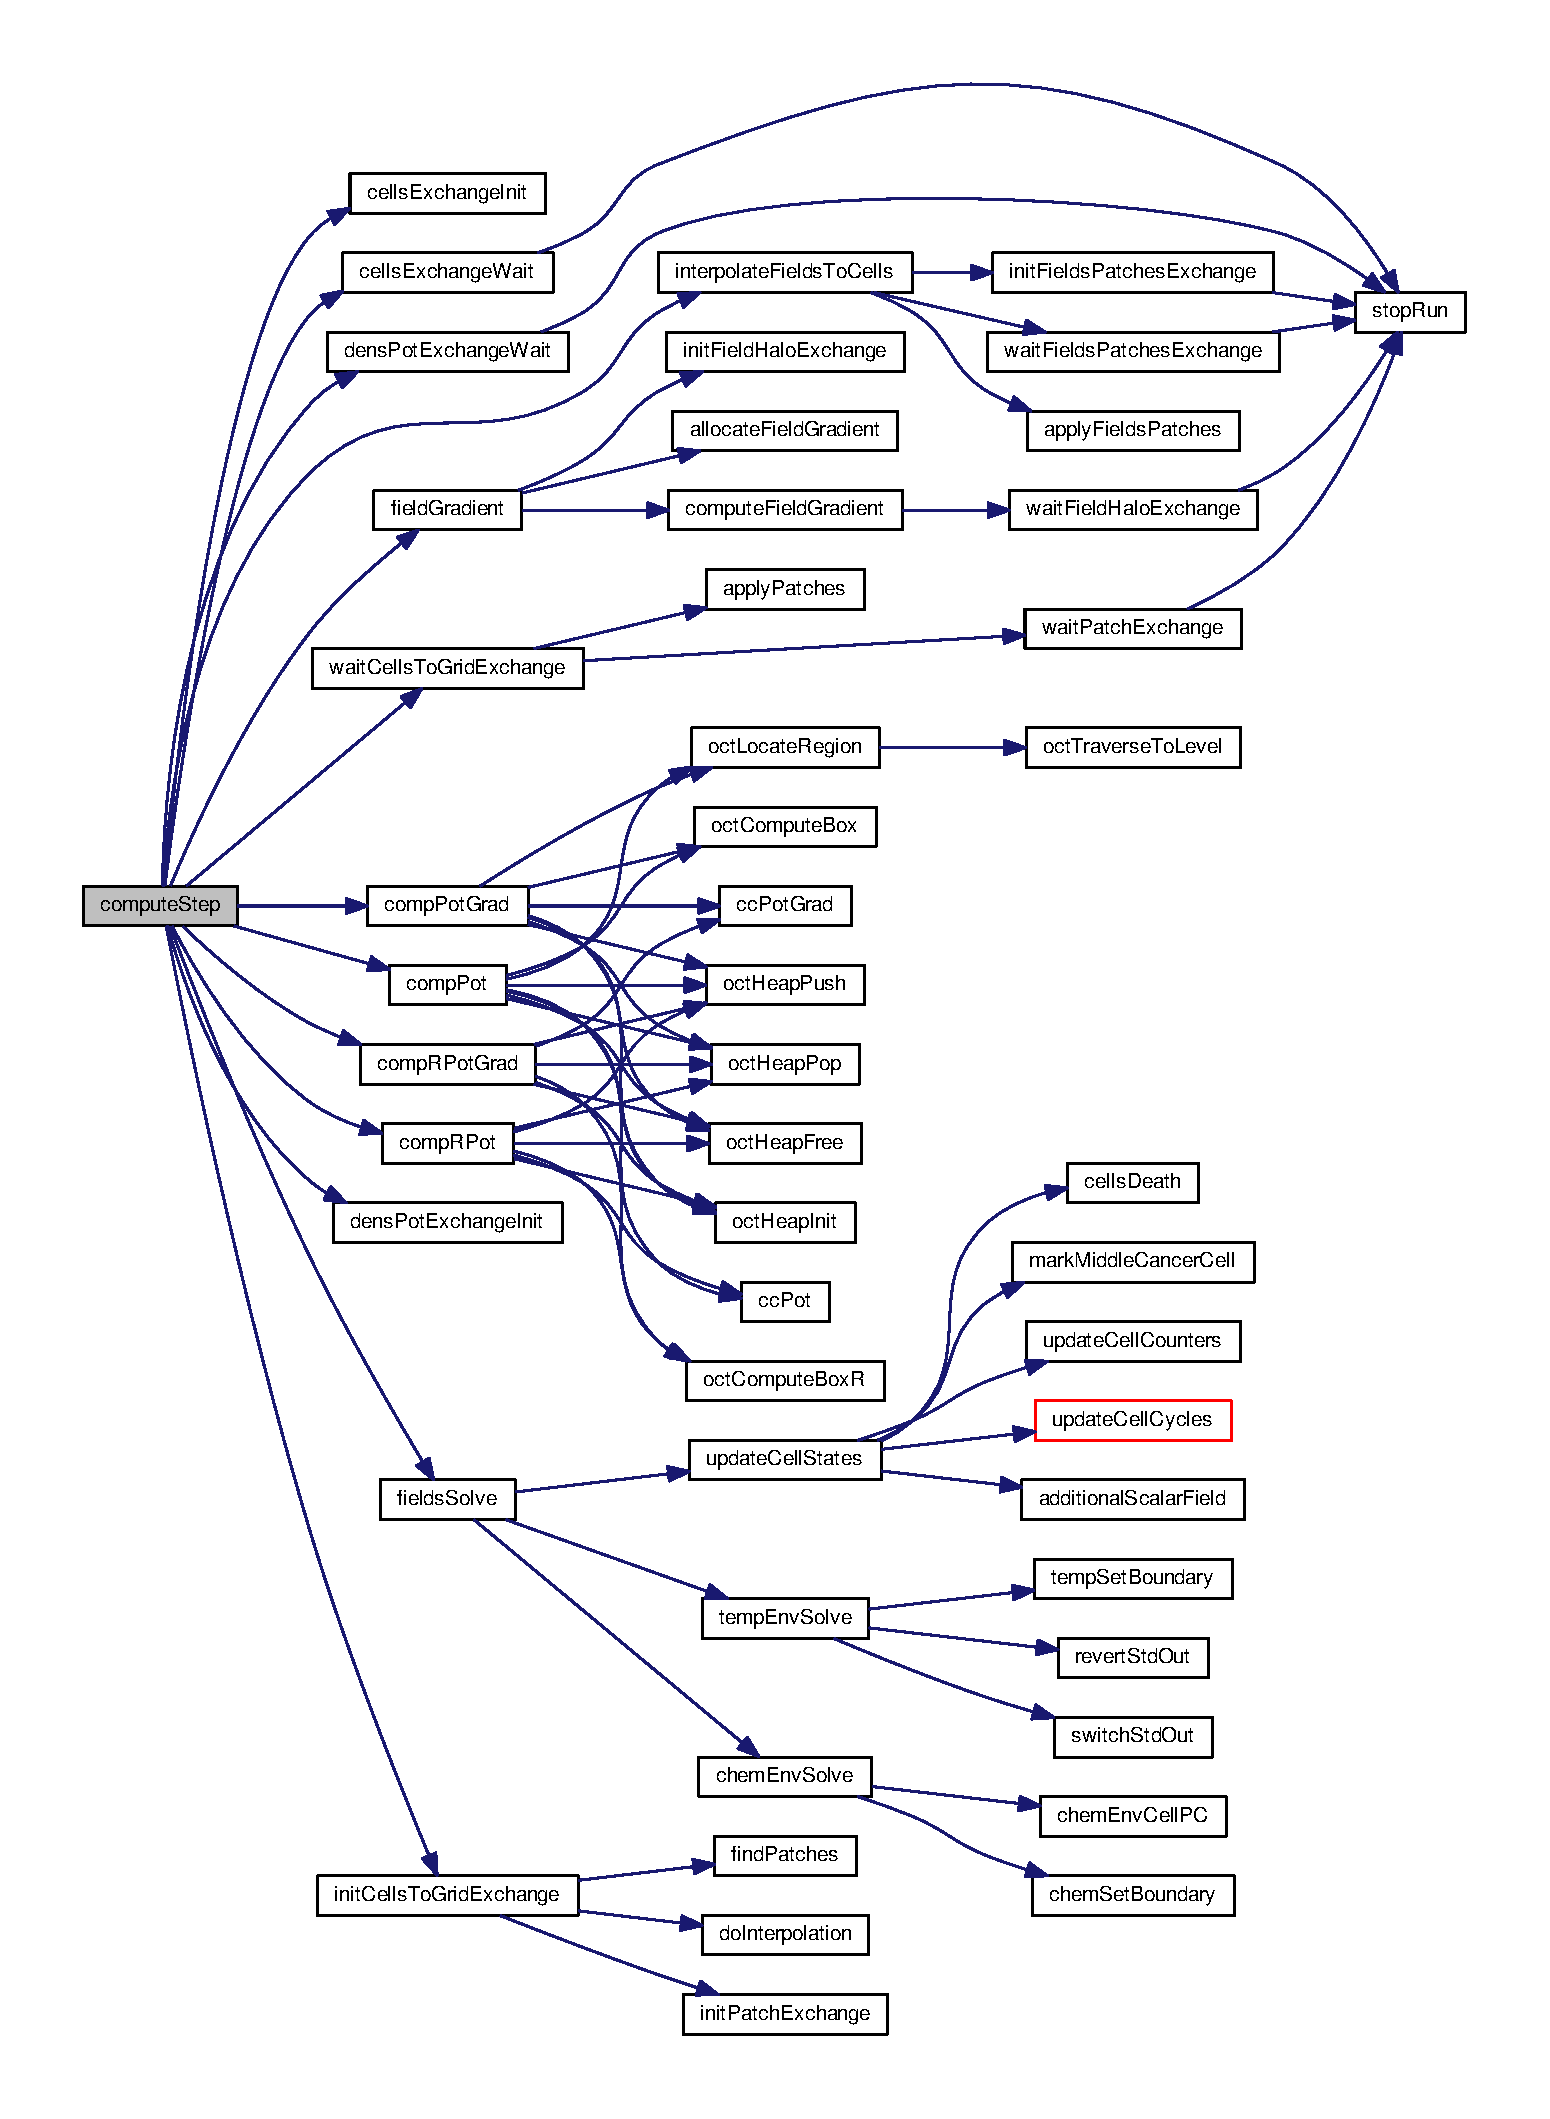
\includegraphics[width=350pt]{compute_8c_ae9a79d8510c24a987ad95d908ad4eb50_cgraph}
\end{center}
\end{figure}




Here is the caller graph for this function\-:\nopagebreak
\begin{figure}[H]
\begin{center}
\leavevmode
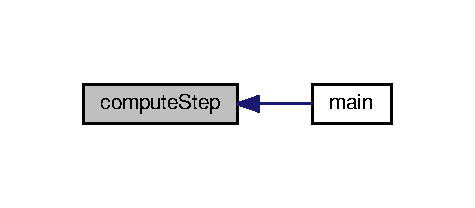
\includegraphics[width=228pt]{compute_8c_ae9a79d8510c24a987ad95d908ad4eb50_icgraph}
\end{center}
\end{figure}



\hypertarget{domdec_8c}{\section{domdec.\-c File Reference}
\label{domdec_8c}\index{domdec.\-c@{domdec.\-c}}
}


contains domain decomposition functions  


{\ttfamily \#include $<$stdio.\-h$>$}\\*
{\ttfamily \#include $<$stdlib.\-h$>$}\\*
{\ttfamily \#include \char`\"{}global.\-h\char`\"{}}\\*
Include dependency graph for domdec.\-c\-:\nopagebreak
\begin{figure}[H]
\begin{center}
\leavevmode
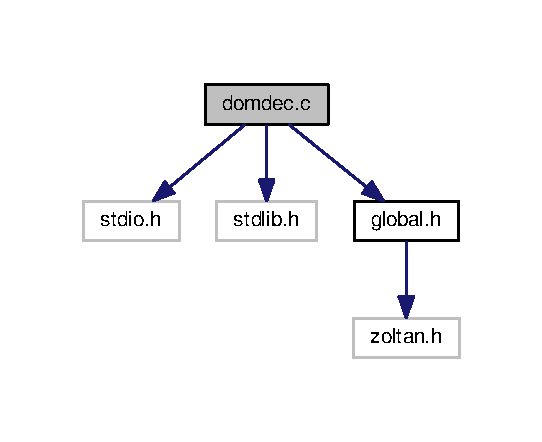
\includegraphics[width=260pt]{domdec_8c__incl}
\end{center}
\end{figure}
\subsection*{Functions}
\begin{DoxyCompactItemize}
\item 
int \hyperlink{domdec_8c_a646b3eaec99bfd258f4353ef2776d7eb}{ztn\-Return\-Dimension} (void $\ast$data, int $\ast$ierr)
\item 
void \hyperlink{domdec_8c_a5494b88a5d3049ebdaff2db552b62d88}{ztn\-Return\-Coords} (void $\ast$data, int \hyperlink{domdec_8c_a6c9a41a72d3fd2ab972e0ccfee7394ad}{num\-Gid\-Entries}, int \hyperlink{domdec_8c_ad836388e3004c88ef80be4e1cef479a5}{num\-Lid\-Entries}, Z\-O\-L\-T\-A\-N\-\_\-\-I\-D\-\_\-\-P\-T\-R global\-Id, Z\-O\-L\-T\-A\-N\-\_\-\-I\-D\-\_\-\-P\-T\-R local\-Id, double $\ast$geom\-Vec, int $\ast$ierr)
\item 
int \hyperlink{domdec_8c_ae16f55406fa663893e53bff6ec0d2891}{ztn\-Return\-Num\-Node} (void $\ast$data, int $\ast$ierr)
\item 
void \hyperlink{domdec_8c_afa9ccb22c460f072633a1033367a5da6}{ztn\-Return\-Owned\-Nodes} (void $\ast$data, int num\-G\-Id\-Entries, int num\-L\-Id\-Entries, Z\-O\-L\-T\-A\-N\-\_\-\-I\-D\-\_\-\-P\-T\-R global\-Ids, Z\-O\-L\-T\-A\-N\-\_\-\-I\-D\-\_\-\-P\-T\-R local\-Ids, int wgt\-Dim, float $\ast$obj\-Wgts, int $\ast$ierr)
\item 
int \hyperlink{domdec_8c_ae8ccac1e6575ca1ebe6ec4e9fde3625c}{ztn\-Return\-Particle\-Data\-Size} (void $\ast$data, int num\-G\-Id\-Entries, int num\-L\-Id\-Entries, Z\-O\-L\-T\-A\-N\-\_\-\-I\-D\-\_\-\-P\-T\-R global\-Id, Z\-O\-L\-T\-A\-N\-\_\-\-I\-D\-\_\-\-P\-T\-R local\-Id, int $\ast$ierr)
\item 
void \hyperlink{domdec_8c_a83bdab74033e8f1fb8a004c3f6a3b76c}{ztn\-Pack} (void $\ast$data, int num\-G\-Id\-Entries, int num\-L\-Id\-Entries, Z\-O\-L\-T\-A\-N\-\_\-\-I\-D\-\_\-\-P\-T\-R global\-Id, Z\-O\-L\-T\-A\-N\-\_\-\-I\-D\-\_\-\-P\-T\-R local\-Id, int dest, int size, char $\ast$buf, int $\ast$ierr)
\item 
void \hyperlink{domdec_8c_a7bb302f4a0beaad9c7c4f08162f1d66c}{ztn\-Pre} (void $\ast$data, int num\-G\-Id\-Entries, int num\-L\-Id\-Entries, int \hyperlink{domdec_8c_a63327cbfe51b3be8ccd7bd7947cf7768}{num\-Import}, Z\-O\-L\-T\-A\-N\-\_\-\-I\-D\-\_\-\-P\-T\-R import\-Global\-Ids, Z\-O\-L\-T\-A\-N\-\_\-\-I\-D\-\_\-\-P\-T\-R import\-Local\-Ids, int $\ast$\hyperlink{domdec_8c_aaf98961d02a34fd945de59d736ba66ce}{import\-Procs}, int $\ast$\hyperlink{domdec_8c_ac2fd1e8fdcde7633cb12cc36b7ffadc6}{import\-To\-Part}, int \hyperlink{domdec_8c_a71a7ca2f86ef16edaf1df524273e642a}{num\-Export}, Z\-O\-L\-T\-A\-N\-\_\-\-I\-D\-\_\-\-P\-T\-R export\-Global\-Ids, Z\-O\-L\-T\-A\-N\-\_\-\-I\-D\-\_\-\-P\-T\-R export\-Local\-Ids, int $\ast$\hyperlink{domdec_8c_a6992b2911e471d2452c8803e182fa4f1}{export\-Procs}, int $\ast$\hyperlink{domdec_8c_a51f5ba020bbcf6108262761504f19ed9}{export\-To\-Part}, int $\ast$ierr)
\item 
void \hyperlink{domdec_8c_aa46ced13f5fc202c3fcc841ff962a565}{ztn\-Mid} (void $\ast$data, int num\-G\-Id\-Entries, int num\-L\-Id\-Entries, int \hyperlink{domdec_8c_a63327cbfe51b3be8ccd7bd7947cf7768}{num\-Import}, Z\-O\-L\-T\-A\-N\-\_\-\-I\-D\-\_\-\-P\-T\-R import\-Global\-Ids, Z\-O\-L\-T\-A\-N\-\_\-\-I\-D\-\_\-\-P\-T\-R import\-Local\-Ids, int $\ast$\hyperlink{domdec_8c_aaf98961d02a34fd945de59d736ba66ce}{import\-Procs}, int $\ast$\hyperlink{domdec_8c_ac2fd1e8fdcde7633cb12cc36b7ffadc6}{import\-To\-Part}, int \hyperlink{domdec_8c_a71a7ca2f86ef16edaf1df524273e642a}{num\-Export}, Z\-O\-L\-T\-A\-N\-\_\-\-I\-D\-\_\-\-P\-T\-R export\-Global\-Ids, Z\-O\-L\-T\-A\-N\-\_\-\-I\-D\-\_\-\-P\-T\-R export\-Local\-Ids, int $\ast$\hyperlink{domdec_8c_a6992b2911e471d2452c8803e182fa4f1}{export\-Procs}, int $\ast$\hyperlink{domdec_8c_a51f5ba020bbcf6108262761504f19ed9}{export\-To\-Part}, int $\ast$ierr)
\item 
void \hyperlink{domdec_8c_a1e5da8ea3ac86aa8c5f131199f20e48d}{ztn\-Post} (void $\ast$data, int num\-G\-Id\-Entries, int num\-L\-Id\-Entries, int \hyperlink{domdec_8c_a63327cbfe51b3be8ccd7bd7947cf7768}{num\-Import}, Z\-O\-L\-T\-A\-N\-\_\-\-I\-D\-\_\-\-P\-T\-R import\-Global\-Ids, Z\-O\-L\-T\-A\-N\-\_\-\-I\-D\-\_\-\-P\-T\-R import\-Local\-Ids, int $\ast$\hyperlink{domdec_8c_aaf98961d02a34fd945de59d736ba66ce}{import\-Procs}, int $\ast$\hyperlink{domdec_8c_ac2fd1e8fdcde7633cb12cc36b7ffadc6}{import\-To\-Part}, int \hyperlink{domdec_8c_a71a7ca2f86ef16edaf1df524273e642a}{num\-Export}, Z\-O\-L\-T\-A\-N\-\_\-\-I\-D\-\_\-\-P\-T\-R export\-Global\-Ids, Z\-O\-L\-T\-A\-N\-\_\-\-I\-D\-\_\-\-P\-T\-R export\-Local\-Ids, int $\ast$\hyperlink{domdec_8c_a6992b2911e471d2452c8803e182fa4f1}{export\-Procs}, int $\ast$\hyperlink{domdec_8c_a51f5ba020bbcf6108262761504f19ed9}{export\-To\-Part}, int $\ast$ierr)
\item 
void \hyperlink{domdec_8c_aa2a71d2700b18abb4e381358df6967c5}{ztn\-Unpack} (void $\ast$data, int num\-G\-Id\-Entries, Z\-O\-L\-T\-A\-N\-\_\-\-I\-D\-\_\-\-P\-T\-R global\-Id, int size, char $\ast$buf, int $\ast$ierr)
\item 
void \hyperlink{domdec_8c_ae7429f968958e491ffc5aa144f564e0a}{decomposition\-Init} (int argc, char $\ast$$\ast$argv, M\-P\-I\-\_\-\-Comm Comm)
\item 
void \hyperlink{domdec_8c_aa62cb73f52f03ee27da62ae952212ceb}{decomposition\-Execute} ()
\item 
void \hyperlink{domdec_8c_a8dd9c084f2af53a06d1629e840f13ee8}{decomposition\-Finalize} ()
\end{DoxyCompactItemize}
\subsection*{Variables}
\begin{DoxyCompactItemize}
\item 
int \hyperlink{domdec_8c_a428798c15a127930411bd3af43e3cdc7}{changes}
\item 
int \hyperlink{domdec_8c_a6c9a41a72d3fd2ab972e0ccfee7394ad}{num\-Gid\-Entries}
\item 
int \hyperlink{domdec_8c_ad836388e3004c88ef80be4e1cef479a5}{num\-Lid\-Entries}
\item 
int \hyperlink{domdec_8c_a63327cbfe51b3be8ccd7bd7947cf7768}{num\-Import}
\item 
Z\-O\-L\-T\-A\-N\-\_\-\-I\-D\-\_\-\-P\-T\-R \hyperlink{domdec_8c_a7003e8d463d214680ced99e92a4e23c4}{import\-Global\-Gids}
\item 
Z\-O\-L\-T\-A\-N\-\_\-\-I\-D\-\_\-\-P\-T\-R \hyperlink{domdec_8c_a1ac001377defa550d2fe2627224ddb46}{import\-Local\-Gids}
\item 
int $\ast$ \hyperlink{domdec_8c_aaf98961d02a34fd945de59d736ba66ce}{import\-Procs}
\item 
int $\ast$ \hyperlink{domdec_8c_ac2fd1e8fdcde7633cb12cc36b7ffadc6}{import\-To\-Part}
\item 
int \hyperlink{domdec_8c_a71a7ca2f86ef16edaf1df524273e642a}{num\-Export}
\item 
Z\-O\-L\-T\-A\-N\-\_\-\-I\-D\-\_\-\-P\-T\-R \hyperlink{domdec_8c_ab47ca6ae0018cbdd0cdd75f8bbc1a1ca}{export\-Global\-Gids}
\item 
Z\-O\-L\-T\-A\-N\-\_\-\-I\-D\-\_\-\-P\-T\-R \hyperlink{domdec_8c_a5582bb1e54eaea68a6c2ddba7ab07553}{export\-Local\-Gids}
\item 
int $\ast$ \hyperlink{domdec_8c_a6992b2911e471d2452c8803e182fa4f1}{export\-Procs}
\item 
int $\ast$ \hyperlink{domdec_8c_a51f5ba020bbcf6108262761504f19ed9}{export\-To\-Part}
\end{DoxyCompactItemize}


\subsection{Detailed Description}
contains domain decomposition functions 

Definition in file \hyperlink{domdec_8c_source}{domdec.\-c}.



\subsection{Function Documentation}
\hypertarget{domdec_8c_aa62cb73f52f03ee27da62ae952212ceb}{\index{domdec.\-c@{domdec.\-c}!decomposition\-Execute@{decomposition\-Execute}}
\index{decomposition\-Execute@{decomposition\-Execute}!domdec.c@{domdec.\-c}}
\subsubsection[{decomposition\-Execute}]{\setlength{\rightskip}{0pt plus 5cm}void decomposition\-Execute (
\begin{DoxyParamCaption}
{}
\end{DoxyParamCaption}
)}}\label{domdec_8c_aa62cb73f52f03ee27da62ae952212ceb}
This function calls the Zoltan's domain decomposition and migration functions. It is called at the beginning of each simulation step. 

Definition at line 240 of file domdec.\-c.



References changes, export\-Global\-Gids, export\-Local\-Gids, export\-Procs, export\-To\-Part, import\-Global\-Gids, import\-Local\-Gids, import\-Procs, import\-To\-Part, M\-P\-Isize, nc, num\-Export, num\-Gid\-Entries, num\-Import, num\-Lid\-Entries, stop\-Run(), and ztn.


\begin{DoxyCode}
241 \{
242   \textcolor{keywordtype}{int} rc;
243 
244   \textcolor{keywordflow}{if} (\hyperlink{global_8h_a0845b4b004824f1fe3cd69db1672fa15}{nc} < \hyperlink{global_8h_a0d7d02544d01ceac87c9d5cadc3af0df}{MPIsize})
245     \textcolor{keywordflow}{return};
246 
247   rc = Zoltan\_LB\_Partition(\hyperlink{global_8h_afc06c50b11f3b60d3738e669b612eb9c}{ztn},  \textcolor{comment}{/* input (all remaining fields are output) */}
248                            &\hyperlink{domdec_8c_a428798c15a127930411bd3af43e3cdc7}{changes}, \textcolor{comment}{/* 1 if partitioning was changed, 0 otherwise */}
249                            &\hyperlink{domdec_8c_a6c9a41a72d3fd2ab972e0ccfee7394ad}{numGidEntries}, \textcolor{comment}{/* number of integers used for a global ID */}
250                            &\hyperlink{domdec_8c_ad836388e3004c88ef80be4e1cef479a5}{numLidEntries}, \textcolor{comment}{/* number of integers used for a local ID */}
251                            &\hyperlink{domdec_8c_a63327cbfe51b3be8ccd7bd7947cf7768}{numImport}, \textcolor{comment}{/* number of objects to be sent to me */}
252                            &\hyperlink{domdec_8c_a7003e8d463d214680ced99e92a4e23c4}{importGlobalGids},   \textcolor{comment}{/* global IDs of objects to be sent to me 
      */}
253                            &\hyperlink{domdec_8c_a1ac001377defa550d2fe2627224ddb46}{importLocalGids}, \textcolor{comment}{/* local IDs of objects to be sent to me */}
254                            &\hyperlink{domdec_8c_aaf98961d02a34fd945de59d736ba66ce}{importProcs}, \textcolor{comment}{/* process rank for source of each incoming object */}
255                            &\hyperlink{domdec_8c_ac2fd1e8fdcde7633cb12cc36b7ffadc6}{importToPart},   \textcolor{comment}{/* new partition for each incoming object */}
256                            &\hyperlink{domdec_8c_a71a7ca2f86ef16edaf1df524273e642a}{numExport}, \textcolor{comment}{/* number of objects I must send to other processes */}
257                            &\hyperlink{domdec_8c_ab47ca6ae0018cbdd0cdd75f8bbc1a1ca}{exportGlobalGids},   \textcolor{comment}{/* global IDs of the objects I must send */}
258                            &\hyperlink{domdec_8c_a5582bb1e54eaea68a6c2ddba7ab07553}{exportLocalGids}, \textcolor{comment}{/* local IDs of the objects I must send */}
259                            &\hyperlink{domdec_8c_a6992b2911e471d2452c8803e182fa4f1}{exportProcs}, \textcolor{comment}{/* process to which I send each of the objects */}
260                            &\hyperlink{domdec_8c_a51f5ba020bbcf6108262761504f19ed9}{exportToPart});  \textcolor{comment}{/* partition to which each object will belong */}
261 
262   \textcolor{keywordflow}{if} (rc != ZOLTAN\_OK)
263     \hyperlink{utils_8c_a07dd99a04f2723be164531a7a862fb67}{stopRun}(112, NULL, \_\_FILE\_\_, \_\_LINE\_\_);
264 
265   \textcolor{comment}{/* free the arrays allocated by Zoltan\_LB\_Partiotion */}
266   Zoltan\_LB\_Free\_Part(&\hyperlink{domdec_8c_a7003e8d463d214680ced99e92a4e23c4}{importGlobalGids}, &\hyperlink{domdec_8c_a1ac001377defa550d2fe2627224ddb46}{importLocalGids}, &
      \hyperlink{domdec_8c_aaf98961d02a34fd945de59d736ba66ce}{importProcs},
267                       &\hyperlink{domdec_8c_ac2fd1e8fdcde7633cb12cc36b7ffadc6}{importToPart});
268   Zoltan\_LB\_Free\_Part(&\hyperlink{domdec_8c_ab47ca6ae0018cbdd0cdd75f8bbc1a1ca}{exportGlobalGids}, &\hyperlink{domdec_8c_a5582bb1e54eaea68a6c2ddba7ab07553}{exportLocalGids}, &
      \hyperlink{domdec_8c_a6992b2911e471d2452c8803e182fa4f1}{exportProcs},
269                       &\hyperlink{domdec_8c_a51f5ba020bbcf6108262761504f19ed9}{exportToPart});
270 \}
\end{DoxyCode}


Here is the call graph for this function\-:\nopagebreak
\begin{figure}[H]
\begin{center}
\leavevmode
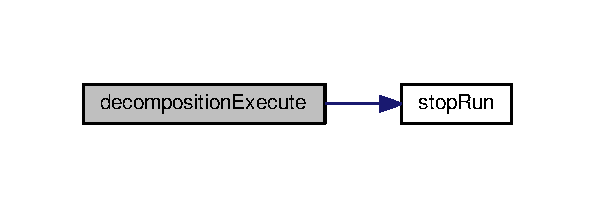
\includegraphics[width=286pt]{domdec_8c_aa62cb73f52f03ee27da62ae952212ceb_cgraph}
\end{center}
\end{figure}




Here is the caller graph for this function\-:\nopagebreak
\begin{figure}[H]
\begin{center}
\leavevmode
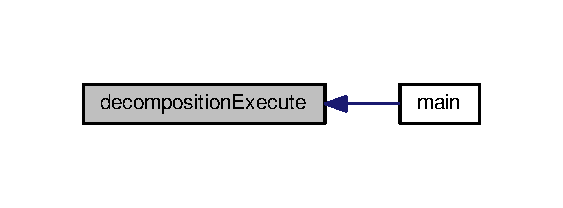
\includegraphics[width=270pt]{domdec_8c_aa62cb73f52f03ee27da62ae952212ceb_icgraph}
\end{center}
\end{figure}


\hypertarget{domdec_8c_a8dd9c084f2af53a06d1629e840f13ee8}{\index{domdec.\-c@{domdec.\-c}!decomposition\-Finalize@{decomposition\-Finalize}}
\index{decomposition\-Finalize@{decomposition\-Finalize}!domdec.c@{domdec.\-c}}
\subsubsection[{decomposition\-Finalize}]{\setlength{\rightskip}{0pt plus 5cm}void decomposition\-Finalize (
\begin{DoxyParamCaption}
{}
\end{DoxyParamCaption}
)}}\label{domdec_8c_a8dd9c084f2af53a06d1629e840f13ee8}
This function deactivates the Zoltan library. It is called at the end of the simulation. 

Definition at line 276 of file domdec.\-c.



References ztn.


\begin{DoxyCode}
277 \{
278   Zoltan\_Destroy(&\hyperlink{global_8h_afc06c50b11f3b60d3738e669b612eb9c}{ztn});
279 \}
\end{DoxyCode}


Here is the caller graph for this function\-:\nopagebreak
\begin{figure}[H]
\begin{center}
\leavevmode
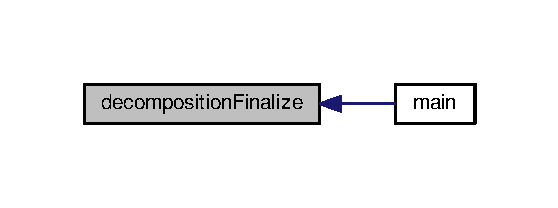
\includegraphics[width=268pt]{domdec_8c_a8dd9c084f2af53a06d1629e840f13ee8_icgraph}
\end{center}
\end{figure}


\hypertarget{domdec_8c_ae7429f968958e491ffc5aa144f564e0a}{\index{domdec.\-c@{domdec.\-c}!decomposition\-Init@{decomposition\-Init}}
\index{decomposition\-Init@{decomposition\-Init}!domdec.c@{domdec.\-c}}
\subsubsection[{decomposition\-Init}]{\setlength{\rightskip}{0pt plus 5cm}void decomposition\-Init (
\begin{DoxyParamCaption}
\item[{int}]{argc, }
\item[{char $\ast$$\ast$}]{argv, }
\item[{M\-P\-I\-\_\-\-Comm}]{Comm}
\end{DoxyParamCaption}
)}}\label{domdec_8c_ae7429f968958e491ffc5aa144f564e0a}
This function initializes the Zoltan library. It is called at the beginning of the simulation. 

Definition at line 191 of file domdec.\-c.



References cells, M\-P\-Irank, stop\-Run(), ztn, ztn\-Mid(), ztn\-Pack(), ztn\-Post(), ztn\-Pre(), ztn\-Return\-Coords(), ztn\-Return\-Dimension(), ztn\-Return\-Num\-Node(), ztn\-Return\-Owned\-Nodes(), ztn\-Return\-Particle\-Data\-Size(), and ztn\-Unpack().


\begin{DoxyCode}
192 \{
193   \textcolor{keywordtype}{int} rc;
194   \textcolor{keywordtype}{float} version;
195 
196   rc = Zoltan\_Initialize(argc, argv, &version);
197   \textcolor{keywordflow}{if} (rc != ZOLTAN\_OK)
198     \hyperlink{utils_8c_a07dd99a04f2723be164531a7a862fb67}{stopRun}(112, NULL, \_\_FILE\_\_, \_\_LINE\_\_);
199 
200   \textcolor{keywordflow}{if} (\hyperlink{global_8h_a710288ab7d2734acc4566a87a645325d}{MPIrank} == 0)
201     printf(\textcolor{stringliteral}{"Zoltan Version %.3f. Initialized.\(\backslash\)n"}, version);
202 
203   \hyperlink{global_8h_afc06c50b11f3b60d3738e669b612eb9c}{ztn} = Zoltan\_Create(MPI\_COMM\_WORLD);
204 
205   Zoltan\_Set\_Param(\hyperlink{global_8h_afc06c50b11f3b60d3738e669b612eb9c}{ztn}, \textcolor{stringliteral}{"IMBALANCE\_TOL"}, \textcolor{stringliteral}{"1.4"});
206   Zoltan\_Set\_Param(\hyperlink{global_8h_afc06c50b11f3b60d3738e669b612eb9c}{ztn}, \textcolor{stringliteral}{"LB\_METHOD"}, \textcolor{stringliteral}{"HSFC"});    \textcolor{comment}{/* Hilbert Space-Filling Curve Partitioning */}
207   Zoltan\_Set\_Param(\hyperlink{global_8h_afc06c50b11f3b60d3738e669b612eb9c}{ztn}, \textcolor{stringliteral}{"NUM\_GID\_ENTRIES"}, \textcolor{stringliteral}{"1"}); \textcolor{comment}{/* global ID is 1 integer */}
208   Zoltan\_Set\_Param(\hyperlink{global_8h_afc06c50b11f3b60d3738e669b612eb9c}{ztn}, \textcolor{stringliteral}{"NUM\_LID\_ENTRIES"}, \textcolor{stringliteral}{"1"}); \textcolor{comment}{/* local ID is 1 integer */}
209   Zoltan\_Set\_Param(\hyperlink{global_8h_afc06c50b11f3b60d3738e669b612eb9c}{ztn}, \textcolor{stringliteral}{"OBJ\_WEIGHT\_DIM"}, \textcolor{stringliteral}{"1"});  \textcolor{comment}{/* we use object weights */}
210   Zoltan\_Set\_Param(\hyperlink{global_8h_afc06c50b11f3b60d3738e669b612eb9c}{ztn}, \textcolor{stringliteral}{"DEBUG\_LEVEL"}, \textcolor{stringliteral}{"0"}); \textcolor{comment}{/* quiet mode; no output unless an error or warning is
       produced */}
211   Zoltan\_Set\_Param(\hyperlink{global_8h_afc06c50b11f3b60d3738e669b612eb9c}{ztn}, \textcolor{stringliteral}{"KEEP\_CUTS"}, \textcolor{stringliteral}{"1"});   \textcolor{comment}{/* save the cuts for later use */}
212   Zoltan\_Set\_Param(\hyperlink{global_8h_afc06c50b11f3b60d3738e669b612eb9c}{ztn}, \textcolor{stringliteral}{"AUTO\_MIGRATE"}, \textcolor{stringliteral}{"1"});    \textcolor{comment}{/* use the auto migration mechanism */}
213 
214   Zoltan\_Set\_Fn(\hyperlink{global_8h_afc06c50b11f3b60d3738e669b612eb9c}{ztn}, ZOLTAN\_NUM\_GEOM\_FN\_TYPE,
215                 (\textcolor{keywordtype}{void} (*)()) \hyperlink{domdec_8c_a646b3eaec99bfd258f4353ef2776d7eb}{ztnReturnDimension}, \hyperlink{global_8h_a3ea537bde8d64e54770a2bd81e3f00be}{cells});
216   Zoltan\_Set\_Fn(\hyperlink{global_8h_afc06c50b11f3b60d3738e669b612eb9c}{ztn}, ZOLTAN\_GEOM\_FN\_TYPE, (\textcolor{keywordtype}{void} (*)()) \hyperlink{domdec_8c_a5494b88a5d3049ebdaff2db552b62d88}{ztnReturnCoords},
217                 \hyperlink{global_8h_a3ea537bde8d64e54770a2bd81e3f00be}{cells});
218   Zoltan\_Set\_Fn(\hyperlink{global_8h_afc06c50b11f3b60d3738e669b612eb9c}{ztn}, ZOLTAN\_NUM\_OBJ\_FN\_TYPE, (\textcolor{keywordtype}{void} (*)()) \hyperlink{domdec_8c_ae16f55406fa663893e53bff6ec0d2891}{ztnReturnNumNode},
219                 \hyperlink{global_8h_a3ea537bde8d64e54770a2bd81e3f00be}{cells});
220   Zoltan\_Set\_Fn(\hyperlink{global_8h_afc06c50b11f3b60d3738e669b612eb9c}{ztn}, ZOLTAN\_OBJ\_LIST\_FN\_TYPE,
221                 (\textcolor{keywordtype}{void} (*)()) \hyperlink{domdec_8c_afa9ccb22c460f072633a1033367a5da6}{ztnReturnOwnedNodes}, \hyperlink{global_8h_a3ea537bde8d64e54770a2bd81e3f00be}{cells});
222   Zoltan\_Set\_Fn(\hyperlink{global_8h_afc06c50b11f3b60d3738e669b612eb9c}{ztn}, ZOLTAN\_OBJ\_SIZE\_FN\_TYPE,
223                 (\textcolor{keywordtype}{void} (*)()) \hyperlink{domdec_8c_ae8ccac1e6575ca1ebe6ec4e9fde3625c}{ztnReturnParticleDataSize}, 
      \hyperlink{global_8h_a3ea537bde8d64e54770a2bd81e3f00be}{cells});
224   Zoltan\_Set\_Fn(\hyperlink{global_8h_afc06c50b11f3b60d3738e669b612eb9c}{ztn}, ZOLTAN\_PACK\_OBJ\_FN\_TYPE, (\textcolor{keywordtype}{void} (*)()) \hyperlink{domdec_8c_a83bdab74033e8f1fb8a004c3f6a3b76c}{ztnPack}, 
      \hyperlink{global_8h_a3ea537bde8d64e54770a2bd81e3f00be}{cells});
225   Zoltan\_Set\_Fn(\hyperlink{global_8h_afc06c50b11f3b60d3738e669b612eb9c}{ztn}, ZOLTAN\_UNPACK\_OBJ\_FN\_TYPE, (\textcolor{keywordtype}{void} (*)()) \hyperlink{domdec_8c_aa2a71d2700b18abb4e381358df6967c5}{ztnUnpack},
226                 \hyperlink{global_8h_a3ea537bde8d64e54770a2bd81e3f00be}{cells});
227   Zoltan\_Set\_Fn(\hyperlink{global_8h_afc06c50b11f3b60d3738e669b612eb9c}{ztn}, ZOLTAN\_PRE\_MIGRATE\_PP\_FN\_TYPE, (\textcolor{keywordtype}{void} (*)()) \hyperlink{domdec_8c_a7bb302f4a0beaad9c7c4f08162f1d66c}{ztnPre},
228                 \hyperlink{global_8h_a3ea537bde8d64e54770a2bd81e3f00be}{cells});
229   Zoltan\_Set\_Fn(\hyperlink{global_8h_afc06c50b11f3b60d3738e669b612eb9c}{ztn}, ZOLTAN\_MID\_MIGRATE\_PP\_FN\_TYPE, (\textcolor{keywordtype}{void} (*)()) \hyperlink{domdec_8c_aa46ced13f5fc202c3fcc841ff962a565}{ztnMid},
230                 \hyperlink{global_8h_a3ea537bde8d64e54770a2bd81e3f00be}{cells});
231   Zoltan\_Set\_Fn(\hyperlink{global_8h_afc06c50b11f3b60d3738e669b612eb9c}{ztn}, ZOLTAN\_POST\_MIGRATE\_PP\_FN\_TYPE, (\textcolor{keywordtype}{void} (*)()) \hyperlink{domdec_8c_a1e5da8ea3ac86aa8c5f131199f20e48d}{ztnPost},
232                 \hyperlink{global_8h_a3ea537bde8d64e54770a2bd81e3f00be}{cells});
233 
234 \}
\end{DoxyCode}


Here is the call graph for this function\-:\nopagebreak
\begin{figure}[H]
\begin{center}
\leavevmode
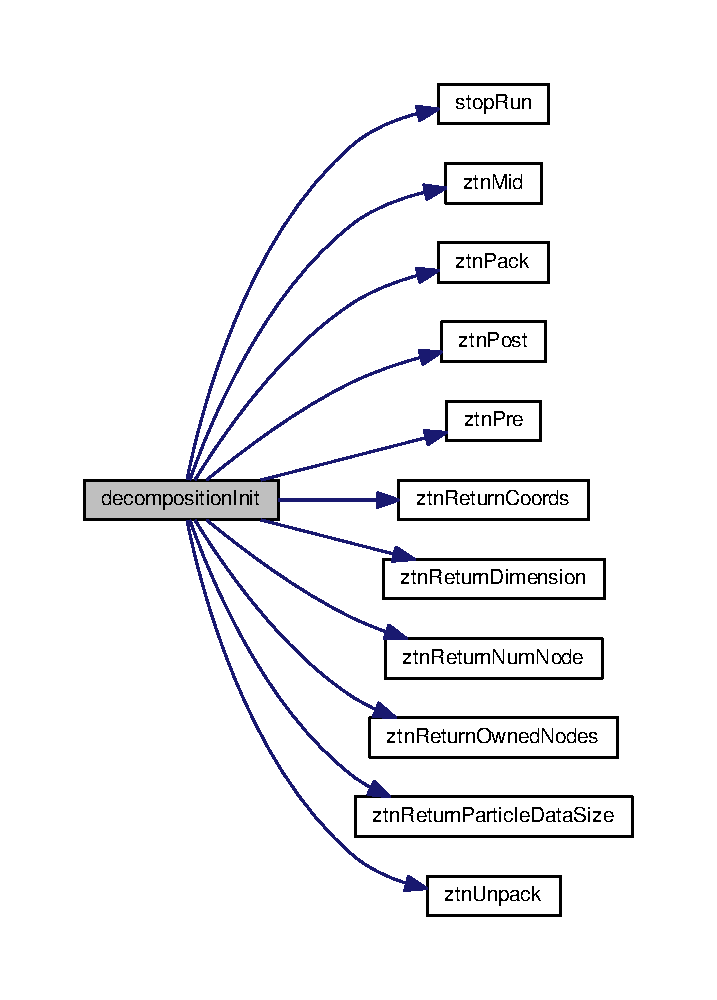
\includegraphics[width=344pt]{domdec_8c_ae7429f968958e491ffc5aa144f564e0a_cgraph}
\end{center}
\end{figure}




Here is the caller graph for this function\-:\nopagebreak
\begin{figure}[H]
\begin{center}
\leavevmode
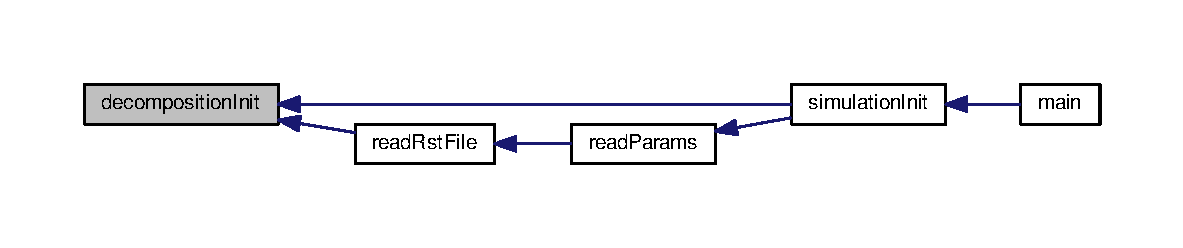
\includegraphics[width=350pt]{domdec_8c_ae7429f968958e491ffc5aa144f564e0a_icgraph}
\end{center}
\end{figure}


\hypertarget{domdec_8c_aa46ced13f5fc202c3fcc841ff962a565}{\index{domdec.\-c@{domdec.\-c}!ztn\-Mid@{ztn\-Mid}}
\index{ztn\-Mid@{ztn\-Mid}!domdec.c@{domdec.\-c}}
\subsubsection[{ztn\-Mid}]{\setlength{\rightskip}{0pt plus 5cm}void ztn\-Mid (
\begin{DoxyParamCaption}
\item[{void $\ast$}]{data, }
\item[{int}]{num\-G\-Id\-Entries, }
\item[{int}]{num\-L\-Id\-Entries, }
\item[{int}]{num\-Import, }
\item[{Z\-O\-L\-T\-A\-N\-\_\-\-I\-D\-\_\-\-P\-T\-R}]{import\-Global\-Ids, }
\item[{Z\-O\-L\-T\-A\-N\-\_\-\-I\-D\-\_\-\-P\-T\-R}]{import\-Local\-Ids, }
\item[{int $\ast$}]{import\-Procs, }
\item[{int $\ast$}]{import\-To\-Part, }
\item[{int}]{num\-Export, }
\item[{Z\-O\-L\-T\-A\-N\-\_\-\-I\-D\-\_\-\-P\-T\-R}]{export\-Global\-Ids, }
\item[{Z\-O\-L\-T\-A\-N\-\_\-\-I\-D\-\_\-\-P\-T\-R}]{export\-Local\-Ids, }
\item[{int $\ast$}]{export\-Procs, }
\item[{int $\ast$}]{export\-To\-Part, }
\item[{int $\ast$}]{ierr}
\end{DoxyParamCaption}
)}}\label{domdec_8c_aa46ced13f5fc202c3fcc841ff962a565}
Zoltan callback function. This function is executed after packing of send buffer and unpacking of receive buffer during migration. 

Definition at line 140 of file domdec.\-c.



References cell\-Data\-::gid, lnc, and num\-Export.


\begin{DoxyCode}
146 \{
147   \textcolor{keywordtype}{int} pos, i;
148   \textcolor{keyword}{struct }\hyperlink{structcellData}{cellData} *c = (\textcolor{keyword}{struct }\hyperlink{structcellData}{cellData} *) data;
149   pos = 0;
150   \textcolor{keywordflow}{for} (i = 0; i < \hyperlink{global_8h_a7065c019590815f10169c219f358e7d0}{lnc}; i++) \{
151     \textcolor{keywordflow}{if} (i != pos && c[i].\hyperlink{structcellData_abb4d4bd9231e9f994e87f32cc4fcfce8}{gid} != -1) \{
152       c[pos] = c[i];
153     \}
154     \textcolor{keywordflow}{if} (c[i].\hyperlink{structcellData_abb4d4bd9231e9f994e87f32cc4fcfce8}{gid} != -1)
155       pos++;
156   \}
157   lnc = lnc - \hyperlink{domdec_8c_a71a7ca2f86ef16edaf1df524273e642a}{numExport};
158 \}
\end{DoxyCode}


Here is the caller graph for this function\-:\nopagebreak
\begin{figure}[H]
\begin{center}
\leavevmode
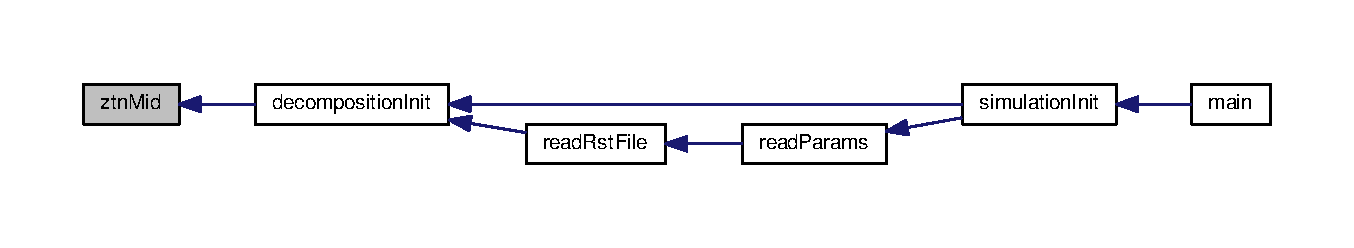
\includegraphics[width=350pt]{domdec_8c_aa46ced13f5fc202c3fcc841ff962a565_icgraph}
\end{center}
\end{figure}


\hypertarget{domdec_8c_a83bdab74033e8f1fb8a004c3f6a3b76c}{\index{domdec.\-c@{domdec.\-c}!ztn\-Pack@{ztn\-Pack}}
\index{ztn\-Pack@{ztn\-Pack}!domdec.c@{domdec.\-c}}
\subsubsection[{ztn\-Pack}]{\setlength{\rightskip}{0pt plus 5cm}void ztn\-Pack (
\begin{DoxyParamCaption}
\item[{void $\ast$}]{data, }
\item[{int}]{num\-G\-Id\-Entries, }
\item[{int}]{num\-L\-Id\-Entries, }
\item[{Z\-O\-L\-T\-A\-N\-\_\-\-I\-D\-\_\-\-P\-T\-R}]{global\-Id, }
\item[{Z\-O\-L\-T\-A\-N\-\_\-\-I\-D\-\_\-\-P\-T\-R}]{local\-Id, }
\item[{int}]{dest, }
\item[{int}]{size, }
\item[{char $\ast$}]{buf, }
\item[{int $\ast$}]{ierr}
\end{DoxyParamCaption}
)}}\label{domdec_8c_a83bdab74033e8f1fb8a004c3f6a3b76c}
Zoltan callback function. This function packs data into a send buffer before migration. 

Definition at line 115 of file domdec.\-c.



References cell\-Data\-::gid.


\begin{DoxyCode}
118 \{
119   \textcolor{keyword}{struct }\hyperlink{structcellData}{cellData} *c = (\textcolor{keyword}{struct }\hyperlink{structcellData}{cellData} *) data;
120   memcpy(buf, &(c[localId[0]]), \textcolor{keyword}{sizeof}(\textcolor{keyword}{struct} \hyperlink{structcellData}{cellData}));
121   c[(int) (*localId)].\hyperlink{structcellData_abb4d4bd9231e9f994e87f32cc4fcfce8}{gid} = -1;  \textcolor{comment}{/* mark local particle as exported */}
122 \}
\end{DoxyCode}


Here is the caller graph for this function\-:\nopagebreak
\begin{figure}[H]
\begin{center}
\leavevmode
\includegraphics[width=350pt]{domdec_8c_a83bdab74033e8f1fb8a004c3f6a3b76c_icgraph}
\end{center}
\end{figure}


\hypertarget{domdec_8c_a1e5da8ea3ac86aa8c5f131199f20e48d}{\index{domdec.\-c@{domdec.\-c}!ztn\-Post@{ztn\-Post}}
\index{ztn\-Post@{ztn\-Post}!domdec.c@{domdec.\-c}}
\subsubsection[{ztn\-Post}]{\setlength{\rightskip}{0pt plus 5cm}void ztn\-Post (
\begin{DoxyParamCaption}
\item[{void $\ast$}]{data, }
\item[{int}]{num\-G\-Id\-Entries, }
\item[{int}]{num\-L\-Id\-Entries, }
\item[{int}]{num\-Import, }
\item[{Z\-O\-L\-T\-A\-N\-\_\-\-I\-D\-\_\-\-P\-T\-R}]{import\-Global\-Ids, }
\item[{Z\-O\-L\-T\-A\-N\-\_\-\-I\-D\-\_\-\-P\-T\-R}]{import\-Local\-Ids, }
\item[{int $\ast$}]{import\-Procs, }
\item[{int $\ast$}]{import\-To\-Part, }
\item[{int}]{num\-Export, }
\item[{Z\-O\-L\-T\-A\-N\-\_\-\-I\-D\-\_\-\-P\-T\-R}]{export\-Global\-Ids, }
\item[{Z\-O\-L\-T\-A\-N\-\_\-\-I\-D\-\_\-\-P\-T\-R}]{export\-Local\-Ids, }
\item[{int $\ast$}]{export\-Procs, }
\item[{int $\ast$}]{export\-To\-Part, }
\item[{int $\ast$}]{ierr}
\end{DoxyParamCaption}
)}}\label{domdec_8c_a1e5da8ea3ac86aa8c5f131199f20e48d}
Zoltan callback function. This function is executed after migration of data between processes. 

Definition at line 163 of file domdec.\-c.



References lnc, and tlnc.


\begin{DoxyCode}
169 \{
170   \textcolor{comment}{/* any post communication operations should go here */}
171   \textcolor{comment}{/* gather number of cells from each process */}
172   MPI\_Allgather(&\hyperlink{global_8h_a7065c019590815f10169c219f358e7d0}{lnc}, 1, MPI\_LONG\_LONG, \hyperlink{global_8h_ac3c96b975a3376c555ad22a7d2688b2f}{tlnc}, 1, MPI\_LONG\_LONG,
173                 MPI\_COMM\_WORLD);
174 \}
\end{DoxyCode}


Here is the caller graph for this function\-:\nopagebreak
\begin{figure}[H]
\begin{center}
\leavevmode
\includegraphics[width=350pt]{domdec_8c_a1e5da8ea3ac86aa8c5f131199f20e48d_icgraph}
\end{center}
\end{figure}


\hypertarget{domdec_8c_a7bb302f4a0beaad9c7c4f08162f1d66c}{\index{domdec.\-c@{domdec.\-c}!ztn\-Pre@{ztn\-Pre}}
\index{ztn\-Pre@{ztn\-Pre}!domdec.c@{domdec.\-c}}
\subsubsection[{ztn\-Pre}]{\setlength{\rightskip}{0pt plus 5cm}void ztn\-Pre (
\begin{DoxyParamCaption}
\item[{void $\ast$}]{data, }
\item[{int}]{num\-G\-Id\-Entries, }
\item[{int}]{num\-L\-Id\-Entries, }
\item[{int}]{num\-Import, }
\item[{Z\-O\-L\-T\-A\-N\-\_\-\-I\-D\-\_\-\-P\-T\-R}]{import\-Global\-Ids, }
\item[{Z\-O\-L\-T\-A\-N\-\_\-\-I\-D\-\_\-\-P\-T\-R}]{import\-Local\-Ids, }
\item[{int $\ast$}]{import\-Procs, }
\item[{int $\ast$}]{import\-To\-Part, }
\item[{int}]{num\-Export, }
\item[{Z\-O\-L\-T\-A\-N\-\_\-\-I\-D\-\_\-\-P\-T\-R}]{export\-Global\-Ids, }
\item[{Z\-O\-L\-T\-A\-N\-\_\-\-I\-D\-\_\-\-P\-T\-R}]{export\-Local\-Ids, }
\item[{int $\ast$}]{export\-Procs, }
\item[{int $\ast$}]{export\-To\-Part, }
\item[{int $\ast$}]{ierr}
\end{DoxyParamCaption}
)}}\label{domdec_8c_a7bb302f4a0beaad9c7c4f08162f1d66c}
Zoltan callback function. This function is executed before migration of data between processes. 

Definition at line 127 of file domdec.\-c.


\begin{DoxyCode}
133 \{
134   \textcolor{comment}{/* any pre communication operations should go here */}
135 \}
\end{DoxyCode}


Here is the caller graph for this function\-:\nopagebreak
\begin{figure}[H]
\begin{center}
\leavevmode
\includegraphics[width=350pt]{domdec_8c_a7bb302f4a0beaad9c7c4f08162f1d66c_icgraph}
\end{center}
\end{figure}


\hypertarget{domdec_8c_a5494b88a5d3049ebdaff2db552b62d88}{\index{domdec.\-c@{domdec.\-c}!ztn\-Return\-Coords@{ztn\-Return\-Coords}}
\index{ztn\-Return\-Coords@{ztn\-Return\-Coords}!domdec.c@{domdec.\-c}}
\subsubsection[{ztn\-Return\-Coords}]{\setlength{\rightskip}{0pt plus 5cm}void ztn\-Return\-Coords (
\begin{DoxyParamCaption}
\item[{void $\ast$}]{data, }
\item[{int}]{num\-Gid\-Entries, }
\item[{int}]{num\-Lid\-Entries, }
\item[{Z\-O\-L\-T\-A\-N\-\_\-\-I\-D\-\_\-\-P\-T\-R}]{global\-Id, }
\item[{Z\-O\-L\-T\-A\-N\-\_\-\-I\-D\-\_\-\-P\-T\-R}]{local\-Id, }
\item[{double $\ast$}]{geom\-Vec, }
\item[{int $\ast$}]{ierr}
\end{DoxyParamCaption}
)}}\label{domdec_8c_a5494b88a5d3049ebdaff2db552b62d88}
Zoltan callback function. This function returns the spatial coordinates of the cell identified by its global and local id. 

Definition at line 62 of file domdec.\-c.



References cells, sdim, cell\-Data\-::x, cell\-Data\-::y, and cell\-Data\-::z.


\begin{DoxyCode}
65 \{
66   \textcolor{keywordflow}{if} (\hyperlink{global_8h_a9fad6472ef73b07a138721c11022697a}{sdim} == 3) \{
67     geomVec[0] = \hyperlink{global_8h_a3ea537bde8d64e54770a2bd81e3f00be}{cells}[localId[0]].\hyperlink{structcellData_af88b946fb90d5f08b5fb740c70e98c10}{x};
68     geomVec[1] = \hyperlink{global_8h_a3ea537bde8d64e54770a2bd81e3f00be}{cells}[localId[0]].\hyperlink{structcellData_ab927965981178aa1fba979a37168db2a}{y};
69     geomVec[2] = \hyperlink{global_8h_a3ea537bde8d64e54770a2bd81e3f00be}{cells}[localId[0]].\hyperlink{structcellData_ab3e6ed577a7c669c19de1f9c1b46c872}{z};
70   \}
71   \textcolor{keywordflow}{if} (\hyperlink{global_8h_a9fad6472ef73b07a138721c11022697a}{sdim} == 2) \{
72     geomVec[0] = \hyperlink{global_8h_a3ea537bde8d64e54770a2bd81e3f00be}{cells}[localId[0]].\hyperlink{structcellData_af88b946fb90d5f08b5fb740c70e98c10}{x};
73     geomVec[1] = \hyperlink{global_8h_a3ea537bde8d64e54770a2bd81e3f00be}{cells}[localId[0]].\hyperlink{structcellData_ab927965981178aa1fba979a37168db2a}{y};
74   \}
75 \}
\end{DoxyCode}


Here is the caller graph for this function\-:\nopagebreak
\begin{figure}[H]
\begin{center}
\leavevmode
\includegraphics[width=350pt]{domdec_8c_a5494b88a5d3049ebdaff2db552b62d88_icgraph}
\end{center}
\end{figure}


\hypertarget{domdec_8c_a646b3eaec99bfd258f4353ef2776d7eb}{\index{domdec.\-c@{domdec.\-c}!ztn\-Return\-Dimension@{ztn\-Return\-Dimension}}
\index{ztn\-Return\-Dimension@{ztn\-Return\-Dimension}!domdec.c@{domdec.\-c}}
\subsubsection[{ztn\-Return\-Dimension}]{\setlength{\rightskip}{0pt plus 5cm}int ztn\-Return\-Dimension (
\begin{DoxyParamCaption}
\item[{void $\ast$}]{data, }
\item[{int $\ast$}]{ierr}
\end{DoxyParamCaption}
)}}\label{domdec_8c_a646b3eaec99bfd258f4353ef2776d7eb}
Zoltan callback function. This function returns the dimension (2\-D or 3\-D) of the system. 

Definition at line 50 of file domdec.\-c.



References sdim.


\begin{DoxyCode}
51 \{
52   \textcolor{keywordflow}{if} (\hyperlink{global_8h_a9fad6472ef73b07a138721c11022697a}{sdim} == 3)
53     \textcolor{keywordflow}{return} 3;
54   \textcolor{keywordflow}{if} (\hyperlink{global_8h_a9fad6472ef73b07a138721c11022697a}{sdim} == 2)
55     \textcolor{keywordflow}{return} 2;
56   \textcolor{keywordflow}{return} 0;
57 \}
\end{DoxyCode}


Here is the caller graph for this function\-:\nopagebreak
\begin{figure}[H]
\begin{center}
\leavevmode
\includegraphics[width=350pt]{domdec_8c_a646b3eaec99bfd258f4353ef2776d7eb_icgraph}
\end{center}
\end{figure}


\hypertarget{domdec_8c_ae16f55406fa663893e53bff6ec0d2891}{\index{domdec.\-c@{domdec.\-c}!ztn\-Return\-Num\-Node@{ztn\-Return\-Num\-Node}}
\index{ztn\-Return\-Num\-Node@{ztn\-Return\-Num\-Node}!domdec.c@{domdec.\-c}}
\subsubsection[{ztn\-Return\-Num\-Node}]{\setlength{\rightskip}{0pt plus 5cm}int ztn\-Return\-Num\-Node (
\begin{DoxyParamCaption}
\item[{void $\ast$}]{data, }
\item[{int $\ast$}]{ierr}
\end{DoxyParamCaption}
)}}\label{domdec_8c_ae16f55406fa663893e53bff6ec0d2891}
Zoltan callback function. This function returns the number of cells assigned to this process. 

Definition at line 80 of file domdec.\-c.



References lnc.


\begin{DoxyCode}
81 \{
82   \textcolor{keywordflow}{return} \hyperlink{global_8h_a7065c019590815f10169c219f358e7d0}{lnc};
83 \}
\end{DoxyCode}


Here is the caller graph for this function\-:\nopagebreak
\begin{figure}[H]
\begin{center}
\leavevmode
\includegraphics[width=350pt]{domdec_8c_ae16f55406fa663893e53bff6ec0d2891_icgraph}
\end{center}
\end{figure}


\hypertarget{domdec_8c_afa9ccb22c460f072633a1033367a5da6}{\index{domdec.\-c@{domdec.\-c}!ztn\-Return\-Owned\-Nodes@{ztn\-Return\-Owned\-Nodes}}
\index{ztn\-Return\-Owned\-Nodes@{ztn\-Return\-Owned\-Nodes}!domdec.c@{domdec.\-c}}
\subsubsection[{ztn\-Return\-Owned\-Nodes}]{\setlength{\rightskip}{0pt plus 5cm}void ztn\-Return\-Owned\-Nodes (
\begin{DoxyParamCaption}
\item[{void $\ast$}]{data, }
\item[{int}]{num\-G\-Id\-Entries, }
\item[{int}]{num\-L\-Id\-Entries, }
\item[{Z\-O\-L\-T\-A\-N\-\_\-\-I\-D\-\_\-\-P\-T\-R}]{global\-Ids, }
\item[{Z\-O\-L\-T\-A\-N\-\_\-\-I\-D\-\_\-\-P\-T\-R}]{local\-Ids, }
\item[{int}]{wgt\-Dim, }
\item[{float $\ast$}]{obj\-Wgts, }
\item[{int $\ast$}]{ierr}
\end{DoxyParamCaption}
)}}\label{domdec_8c_afa9ccb22c460f072633a1033367a5da6}
Zoltan callback function. This function fills the tables of global ids, local ids and weights for all cells assigned to this process. 

Definition at line 88 of file domdec.\-c.



References cells, cell\-Data\-::gid, and lnc.


\begin{DoxyCode}
91 \{
92   \textcolor{keywordtype}{int} i;
93   \textcolor{keywordflow}{for} (i = 0; i < \hyperlink{global_8h_a7065c019590815f10169c219f358e7d0}{lnc}; i++) \{
94     globalIds[i * numGIdEntries] = \hyperlink{global_8h_a3ea537bde8d64e54770a2bd81e3f00be}{cells}[i].\hyperlink{structcellData_abb4d4bd9231e9f994e87f32cc4fcfce8}{gid};
95     localIds[i * numLIdEntries] = i;
96     objWgts[i] = 1.0;
97     \textcolor{comment}{//if(nc==1 || step==0) objWgts[i]=1.0;}
98     \textcolor{comment}{//else objWgts[i]=cells[i].density;}
99   \}
100 \}
\end{DoxyCode}


Here is the caller graph for this function\-:\nopagebreak
\begin{figure}[H]
\begin{center}
\leavevmode
\includegraphics[width=350pt]{domdec_8c_afa9ccb22c460f072633a1033367a5da6_icgraph}
\end{center}
\end{figure}


\hypertarget{domdec_8c_ae8ccac1e6575ca1ebe6ec4e9fde3625c}{\index{domdec.\-c@{domdec.\-c}!ztn\-Return\-Particle\-Data\-Size@{ztn\-Return\-Particle\-Data\-Size}}
\index{ztn\-Return\-Particle\-Data\-Size@{ztn\-Return\-Particle\-Data\-Size}!domdec.c@{domdec.\-c}}
\subsubsection[{ztn\-Return\-Particle\-Data\-Size}]{\setlength{\rightskip}{0pt plus 5cm}int ztn\-Return\-Particle\-Data\-Size (
\begin{DoxyParamCaption}
\item[{void $\ast$}]{data, }
\item[{int}]{num\-G\-Id\-Entries, }
\item[{int}]{num\-L\-Id\-Entries, }
\item[{Z\-O\-L\-T\-A\-N\-\_\-\-I\-D\-\_\-\-P\-T\-R}]{global\-Id, }
\item[{Z\-O\-L\-T\-A\-N\-\_\-\-I\-D\-\_\-\-P\-T\-R}]{local\-Id, }
\item[{int $\ast$}]{ierr}
\end{DoxyParamCaption}
)}}\label{domdec_8c_ae8ccac1e6575ca1ebe6ec4e9fde3625c}
Zoltan callback function. This function returns the size of a data structure used for keeping the data of a single cell. 

Definition at line 105 of file domdec.\-c.


\begin{DoxyCode}
108 \{
109   \textcolor{keywordflow}{return} \textcolor{keyword}{sizeof}(\textcolor{keyword}{struct }\hyperlink{structcellData}{cellData});
110 \}
\end{DoxyCode}


Here is the caller graph for this function\-:\nopagebreak
\begin{figure}[H]
\begin{center}
\leavevmode
\includegraphics[width=350pt]{domdec_8c_ae8ccac1e6575ca1ebe6ec4e9fde3625c_icgraph}
\end{center}
\end{figure}


\hypertarget{domdec_8c_aa2a71d2700b18abb4e381358df6967c5}{\index{domdec.\-c@{domdec.\-c}!ztn\-Unpack@{ztn\-Unpack}}
\index{ztn\-Unpack@{ztn\-Unpack}!domdec.c@{domdec.\-c}}
\subsubsection[{ztn\-Unpack}]{\setlength{\rightskip}{0pt plus 5cm}void ztn\-Unpack (
\begin{DoxyParamCaption}
\item[{void $\ast$}]{data, }
\item[{int}]{num\-G\-Id\-Entries, }
\item[{Z\-O\-L\-T\-A\-N\-\_\-\-I\-D\-\_\-\-P\-T\-R}]{global\-Id, }
\item[{int}]{size, }
\item[{char $\ast$}]{buf, }
\item[{int $\ast$}]{ierr}
\end{DoxyParamCaption}
)}}\label{domdec_8c_aa2a71d2700b18abb4e381358df6967c5}
Zoltan callback function. This function unpacks data from the receive buffer. 

Definition at line 179 of file domdec.\-c.



References lnc.


\begin{DoxyCode}
181 \{
182   \textcolor{keyword}{struct }\hyperlink{structcellData}{cellData} *c = (\textcolor{keyword}{struct }\hyperlink{structcellData}{cellData} *) data;
183   memcpy(&c[\hyperlink{global_8h_a7065c019590815f10169c219f358e7d0}{lnc}], buf, \textcolor{keyword}{sizeof}(\textcolor{keyword}{struct} \hyperlink{structcellData}{cellData}));
184   lnc++;
185 \}
\end{DoxyCode}


Here is the caller graph for this function\-:\nopagebreak
\begin{figure}[H]
\begin{center}
\leavevmode
\includegraphics[width=350pt]{domdec_8c_aa2a71d2700b18abb4e381358df6967c5_icgraph}
\end{center}
\end{figure}




\subsection{Variable Documentation}
\hypertarget{domdec_8c_a428798c15a127930411bd3af43e3cdc7}{\index{domdec.\-c@{domdec.\-c}!changes@{changes}}
\index{changes@{changes}!domdec.c@{domdec.\-c}}
\subsubsection[{changes}]{\setlength{\rightskip}{0pt plus 5cm}int changes}}\label{domdec_8c_a428798c15a127930411bd3af43e3cdc7}


Definition at line 33 of file domdec.\-c.

\hypertarget{domdec_8c_ab47ca6ae0018cbdd0cdd75f8bbc1a1ca}{\index{domdec.\-c@{domdec.\-c}!export\-Global\-Gids@{export\-Global\-Gids}}
\index{export\-Global\-Gids@{export\-Global\-Gids}!domdec.c@{domdec.\-c}}
\subsubsection[{export\-Global\-Gids}]{\setlength{\rightskip}{0pt plus 5cm}Z\-O\-L\-T\-A\-N\-\_\-\-I\-D\-\_\-\-P\-T\-R export\-Global\-Gids}}\label{domdec_8c_ab47ca6ae0018cbdd0cdd75f8bbc1a1ca}


Definition at line 42 of file domdec.\-c.

\hypertarget{domdec_8c_a5582bb1e54eaea68a6c2ddba7ab07553}{\index{domdec.\-c@{domdec.\-c}!export\-Local\-Gids@{export\-Local\-Gids}}
\index{export\-Local\-Gids@{export\-Local\-Gids}!domdec.c@{domdec.\-c}}
\subsubsection[{export\-Local\-Gids}]{\setlength{\rightskip}{0pt plus 5cm}Z\-O\-L\-T\-A\-N\-\_\-\-I\-D\-\_\-\-P\-T\-R export\-Local\-Gids}}\label{domdec_8c_a5582bb1e54eaea68a6c2ddba7ab07553}


Definition at line 43 of file domdec.\-c.

\hypertarget{domdec_8c_a6992b2911e471d2452c8803e182fa4f1}{\index{domdec.\-c@{domdec.\-c}!export\-Procs@{export\-Procs}}
\index{export\-Procs@{export\-Procs}!domdec.c@{domdec.\-c}}
\subsubsection[{export\-Procs}]{\setlength{\rightskip}{0pt plus 5cm}int$\ast$ export\-Procs}}\label{domdec_8c_a6992b2911e471d2452c8803e182fa4f1}


Definition at line 44 of file domdec.\-c.

\hypertarget{domdec_8c_a51f5ba020bbcf6108262761504f19ed9}{\index{domdec.\-c@{domdec.\-c}!export\-To\-Part@{export\-To\-Part}}
\index{export\-To\-Part@{export\-To\-Part}!domdec.c@{domdec.\-c}}
\subsubsection[{export\-To\-Part}]{\setlength{\rightskip}{0pt plus 5cm}int$\ast$ export\-To\-Part}}\label{domdec_8c_a51f5ba020bbcf6108262761504f19ed9}


Definition at line 45 of file domdec.\-c.

\hypertarget{domdec_8c_a7003e8d463d214680ced99e92a4e23c4}{\index{domdec.\-c@{domdec.\-c}!import\-Global\-Gids@{import\-Global\-Gids}}
\index{import\-Global\-Gids@{import\-Global\-Gids}!domdec.c@{domdec.\-c}}
\subsubsection[{import\-Global\-Gids}]{\setlength{\rightskip}{0pt plus 5cm}Z\-O\-L\-T\-A\-N\-\_\-\-I\-D\-\_\-\-P\-T\-R import\-Global\-Gids}}\label{domdec_8c_a7003e8d463d214680ced99e92a4e23c4}


Definition at line 37 of file domdec.\-c.

\hypertarget{domdec_8c_a1ac001377defa550d2fe2627224ddb46}{\index{domdec.\-c@{domdec.\-c}!import\-Local\-Gids@{import\-Local\-Gids}}
\index{import\-Local\-Gids@{import\-Local\-Gids}!domdec.c@{domdec.\-c}}
\subsubsection[{import\-Local\-Gids}]{\setlength{\rightskip}{0pt plus 5cm}Z\-O\-L\-T\-A\-N\-\_\-\-I\-D\-\_\-\-P\-T\-R import\-Local\-Gids}}\label{domdec_8c_a1ac001377defa550d2fe2627224ddb46}


Definition at line 38 of file domdec.\-c.

\hypertarget{domdec_8c_aaf98961d02a34fd945de59d736ba66ce}{\index{domdec.\-c@{domdec.\-c}!import\-Procs@{import\-Procs}}
\index{import\-Procs@{import\-Procs}!domdec.c@{domdec.\-c}}
\subsubsection[{import\-Procs}]{\setlength{\rightskip}{0pt plus 5cm}int$\ast$ import\-Procs}}\label{domdec_8c_aaf98961d02a34fd945de59d736ba66ce}


Definition at line 39 of file domdec.\-c.

\hypertarget{domdec_8c_ac2fd1e8fdcde7633cb12cc36b7ffadc6}{\index{domdec.\-c@{domdec.\-c}!import\-To\-Part@{import\-To\-Part}}
\index{import\-To\-Part@{import\-To\-Part}!domdec.c@{domdec.\-c}}
\subsubsection[{import\-To\-Part}]{\setlength{\rightskip}{0pt plus 5cm}int$\ast$ import\-To\-Part}}\label{domdec_8c_ac2fd1e8fdcde7633cb12cc36b7ffadc6}


Definition at line 40 of file domdec.\-c.

\hypertarget{domdec_8c_a71a7ca2f86ef16edaf1df524273e642a}{\index{domdec.\-c@{domdec.\-c}!num\-Export@{num\-Export}}
\index{num\-Export@{num\-Export}!domdec.c@{domdec.\-c}}
\subsubsection[{num\-Export}]{\setlength{\rightskip}{0pt plus 5cm}int num\-Export}}\label{domdec_8c_a71a7ca2f86ef16edaf1df524273e642a}


Definition at line 41 of file domdec.\-c.

\hypertarget{domdec_8c_a6c9a41a72d3fd2ab972e0ccfee7394ad}{\index{domdec.\-c@{domdec.\-c}!num\-Gid\-Entries@{num\-Gid\-Entries}}
\index{num\-Gid\-Entries@{num\-Gid\-Entries}!domdec.c@{domdec.\-c}}
\subsubsection[{num\-Gid\-Entries}]{\setlength{\rightskip}{0pt plus 5cm}int num\-Gid\-Entries}}\label{domdec_8c_a6c9a41a72d3fd2ab972e0ccfee7394ad}


Definition at line 34 of file domdec.\-c.

\hypertarget{domdec_8c_a63327cbfe51b3be8ccd7bd7947cf7768}{\index{domdec.\-c@{domdec.\-c}!num\-Import@{num\-Import}}
\index{num\-Import@{num\-Import}!domdec.c@{domdec.\-c}}
\subsubsection[{num\-Import}]{\setlength{\rightskip}{0pt plus 5cm}int num\-Import}}\label{domdec_8c_a63327cbfe51b3be8ccd7bd7947cf7768}


Definition at line 36 of file domdec.\-c.

\hypertarget{domdec_8c_ad836388e3004c88ef80be4e1cef479a5}{\index{domdec.\-c@{domdec.\-c}!num\-Lid\-Entries@{num\-Lid\-Entries}}
\index{num\-Lid\-Entries@{num\-Lid\-Entries}!domdec.c@{domdec.\-c}}
\subsubsection[{num\-Lid\-Entries}]{\setlength{\rightskip}{0pt plus 5cm}int num\-Lid\-Entries}}\label{domdec_8c_ad836388e3004c88ef80be4e1cef479a5}


Definition at line 35 of file domdec.\-c.


\hypertarget{fields_8c}{\section{fields.\-c File Reference}
\label{fields_8c}\index{fields.\-c@{fields.\-c}}
}


contains driving functions for the global fields  


{\ttfamily \#include $<$stdio.\-h$>$}\\*
{\ttfamily \#include $<$stdlib.\-h$>$}\\*
{\ttfamily \#include $<$math.\-h$>$}\\*
{\ttfamily \#include \char`\"{}global.\-h\char`\"{}}\\*
{\ttfamily \#include \char`\"{}fields.\-h\char`\"{}}\\*
Include dependency graph for fields.\-c\-:\nopagebreak
\begin{figure}[H]
\begin{center}
\leavevmode
\includegraphics[width=350pt]{fields_8c__incl}
\end{center}
\end{figure}
\subsection*{Functions}
\begin{DoxyCompactItemize}
\item 
void \hyperlink{fields_8c_af20f777e99b72945b22c053d2f7b8e46}{fields\-Init} ()
\item 
void \hyperlink{fields_8c_a8aa63d2a1c91ca03cb71cfc867e40c74}{fields\-Solve} ()
\item 
void \hyperlink{fields_8c_a582e88e9fb1bce076ff733084b35c115}{allocate\-Field\-Gradient} ()
\item 
void \hyperlink{fields_8c_a65a21aa9797f80765a167ebccc923c7f}{init\-Field\-Halo\-Exchange} (int chf)
\item 
void \hyperlink{fields_8c_ad08174d63d4750c8d6661144e3f3bb1c}{wait\-Field\-Halo\-Exchange} ()
\item 
void \hyperlink{fields_8c_ad83000b914316331bf7d3b66c53a289d}{compute\-Field\-Gradient} (int chf)
\item 
void \hyperlink{fields_8c_a2b1cba77aa657bc348ed055d89bfbe50}{field\-Gradient} ()
\end{DoxyCompactItemize}


\subsection{Detailed Description}
contains driving functions for the global fields 

Definition in file \hyperlink{fields_8c_source}{fields.\-c}.



\subsection{Function Documentation}
\hypertarget{fields_8c_a582e88e9fb1bce076ff733084b35c115}{\index{fields.\-c@{fields.\-c}!allocate\-Field\-Gradient@{allocate\-Field\-Gradient}}
\index{allocate\-Field\-Gradient@{allocate\-Field\-Gradient}!fields.c@{fields.\-c}}
\subsubsection[{allocate\-Field\-Gradient}]{\setlength{\rightskip}{0pt plus 5cm}void allocate\-Field\-Gradient (
\begin{DoxyParamCaption}
{}
\end{DoxyParamCaption}
)}}\label{fields_8c_a582e88e9fb1bce076ff733084b35c115}


Definition at line 189 of file fields.\-c.



References gfields, grid\-Size, halo\-R\-X0, halo\-R\-X1, halo\-R\-Y0, halo\-R\-Y1, halo\-R\-Z0, halo\-R\-Z1, halo\-S\-X0, halo\-S\-X1, halo\-S\-Y0, halo\-S\-Y1, halo\-S\-Z0, halo\-S\-Z1, M\-P\-I\-\_\-\-C\-A\-R\-T\-\_\-\-C\-O\-M\-M, r\-X0, r\-X1, r\-Y0, r\-Y1, r\-Z0, r\-Z1, int64\-Vector3d\-::x, int64\-Vector3d\-::y, and int64\-Vector3d\-::z.


\begin{DoxyCode}
190 \{
191 
192   \textcolor{keywordflow}{if} (!\hyperlink{fields_8h_abe4692639a5f11507faff09f2d37efa8}{gfields})
193     \textcolor{keywordflow}{return};
194 
195   MPI\_Cart\_shift(\hyperlink{global_8h_a34ac355617a6a906e1f3e7832aeb0073}{MPI\_CART\_COMM},0,1,&\hyperlink{fields_8h_af04702287d6dec57802c81071212423f}{rX0},&\hyperlink{fields_8h_a7c990eb627c166f119dddf7d0fe33285}{rX1});
196   MPI\_Cart\_shift(\hyperlink{global_8h_a34ac355617a6a906e1f3e7832aeb0073}{MPI\_CART\_COMM},1,1,&\hyperlink{fields_8h_ac41b308e7a718a159727b7a08340b577}{rY0},&\hyperlink{fields_8h_a72bac0e9dbb96427052c46a5dbb5675c}{rY1});
197   MPI\_Cart\_shift(\hyperlink{global_8h_a34ac355617a6a906e1f3e7832aeb0073}{MPI\_CART\_COMM},2,1,&\hyperlink{fields_8h_af48da71f2b169dce2e4ae8da64f79cea}{rZ0},&\hyperlink{fields_8h_a6698e8930956f935b86bf825e333f82e}{rZ1});
198 
199   \textcolor{comment}{/* allocate send buffers */}
200   \textcolor{keywordflow}{if}(\hyperlink{fields_8h_af04702287d6dec57802c81071212423f}{rX0}!=MPI\_PROC\_NULL) \hyperlink{fields_8h_a5b1a6ed0ad91a58cc9c9e48eba217643}{haloSX0}=(\textcolor{keywordtype}{double}*)calloc(\hyperlink{fields_8h_ae67bb9d09bd0919a0ccbc27b387cec72}{gridSize}.\hyperlink{structint64Vector3d_a0cbcba26311a97b8e0763317e105a918}{y}*
      \hyperlink{fields_8h_ae67bb9d09bd0919a0ccbc27b387cec72}{gridSize}.\hyperlink{structint64Vector3d_a44624880ae3bb63041297b70cb33408b}{z},\textcolor{keyword}{sizeof}(\textcolor{keywordtype}{double}));
201   \textcolor{keywordflow}{if}(\hyperlink{fields_8h_a7c990eb627c166f119dddf7d0fe33285}{rX1}!=MPI\_PROC\_NULL) \hyperlink{fields_8h_abcd411d2d371bb75abb7c2d89aac1265}{haloSX1}=(\textcolor{keywordtype}{double}*)calloc(\hyperlink{fields_8h_ae67bb9d09bd0919a0ccbc27b387cec72}{gridSize}.\hyperlink{structint64Vector3d_a0cbcba26311a97b8e0763317e105a918}{y}*
      \hyperlink{fields_8h_ae67bb9d09bd0919a0ccbc27b387cec72}{gridSize}.\hyperlink{structint64Vector3d_a44624880ae3bb63041297b70cb33408b}{z},\textcolor{keyword}{sizeof}(\textcolor{keywordtype}{double}));
202   \textcolor{keywordflow}{if}(\hyperlink{fields_8h_ac41b308e7a718a159727b7a08340b577}{rY0}!=MPI\_PROC\_NULL) \hyperlink{fields_8h_ab8d502d0d87b4e406600573e62b06f28}{haloSY0}=(\textcolor{keywordtype}{double}*)calloc(\hyperlink{fields_8h_ae67bb9d09bd0919a0ccbc27b387cec72}{gridSize}.\hyperlink{structint64Vector3d_a040359f45343ce6667f5c66fda5f50e3}{x}*
      \hyperlink{fields_8h_ae67bb9d09bd0919a0ccbc27b387cec72}{gridSize}.\hyperlink{structint64Vector3d_a44624880ae3bb63041297b70cb33408b}{z},\textcolor{keyword}{sizeof}(\textcolor{keywordtype}{double}));
203   \textcolor{keywordflow}{if}(\hyperlink{fields_8h_a72bac0e9dbb96427052c46a5dbb5675c}{rY1}!=MPI\_PROC\_NULL) \hyperlink{fields_8h_af601c47ad6c97b079ce66bba7e7b2a24}{haloSY1}=(\textcolor{keywordtype}{double}*)calloc(\hyperlink{fields_8h_ae67bb9d09bd0919a0ccbc27b387cec72}{gridSize}.\hyperlink{structint64Vector3d_a040359f45343ce6667f5c66fda5f50e3}{x}*
      \hyperlink{fields_8h_ae67bb9d09bd0919a0ccbc27b387cec72}{gridSize}.\hyperlink{structint64Vector3d_a44624880ae3bb63041297b70cb33408b}{z},\textcolor{keyword}{sizeof}(\textcolor{keywordtype}{double}));
204   \textcolor{keywordflow}{if}(\hyperlink{fields_8h_af48da71f2b169dce2e4ae8da64f79cea}{rZ0}!=MPI\_PROC\_NULL) \hyperlink{fields_8h_a421410f629046ce8c9eaea51123ae34d}{haloSZ0}=(\textcolor{keywordtype}{double}*)calloc(\hyperlink{fields_8h_ae67bb9d09bd0919a0ccbc27b387cec72}{gridSize}.\hyperlink{structint64Vector3d_a0cbcba26311a97b8e0763317e105a918}{y}*
      \hyperlink{fields_8h_ae67bb9d09bd0919a0ccbc27b387cec72}{gridSize}.\hyperlink{structint64Vector3d_a040359f45343ce6667f5c66fda5f50e3}{x},\textcolor{keyword}{sizeof}(\textcolor{keywordtype}{double}));
205   \textcolor{keywordflow}{if}(\hyperlink{fields_8h_a6698e8930956f935b86bf825e333f82e}{rZ1}!=MPI\_PROC\_NULL) \hyperlink{fields_8h_a4e1a5f725f1e3695a8b11d27ac45b905}{haloSZ1}=(\textcolor{keywordtype}{double}*)calloc(\hyperlink{fields_8h_ae67bb9d09bd0919a0ccbc27b387cec72}{gridSize}.\hyperlink{structint64Vector3d_a0cbcba26311a97b8e0763317e105a918}{y}*
      \hyperlink{fields_8h_ae67bb9d09bd0919a0ccbc27b387cec72}{gridSize}.\hyperlink{structint64Vector3d_a040359f45343ce6667f5c66fda5f50e3}{x},\textcolor{keyword}{sizeof}(\textcolor{keywordtype}{double}));
206 
207   \textcolor{comment}{/* allocate receive buffers */}
208   \textcolor{keywordflow}{if}(\hyperlink{fields_8h_af04702287d6dec57802c81071212423f}{rX0}!=MPI\_PROC\_NULL) \hyperlink{fields_8h_aa455b936396c224d389201ecf4b94368}{haloRX0}=(\textcolor{keywordtype}{double}*)calloc(\hyperlink{fields_8h_ae67bb9d09bd0919a0ccbc27b387cec72}{gridSize}.\hyperlink{structint64Vector3d_a0cbcba26311a97b8e0763317e105a918}{y}*
      \hyperlink{fields_8h_ae67bb9d09bd0919a0ccbc27b387cec72}{gridSize}.\hyperlink{structint64Vector3d_a44624880ae3bb63041297b70cb33408b}{z},\textcolor{keyword}{sizeof}(\textcolor{keywordtype}{double}));
209   \textcolor{keywordflow}{if}(\hyperlink{fields_8h_a7c990eb627c166f119dddf7d0fe33285}{rX1}!=MPI\_PROC\_NULL) \hyperlink{fields_8h_a028e4eb118e3c99a36504c722fdd498f}{haloRX1}=(\textcolor{keywordtype}{double}*)calloc(\hyperlink{fields_8h_ae67bb9d09bd0919a0ccbc27b387cec72}{gridSize}.\hyperlink{structint64Vector3d_a0cbcba26311a97b8e0763317e105a918}{y}*
      \hyperlink{fields_8h_ae67bb9d09bd0919a0ccbc27b387cec72}{gridSize}.\hyperlink{structint64Vector3d_a44624880ae3bb63041297b70cb33408b}{z},\textcolor{keyword}{sizeof}(\textcolor{keywordtype}{double}));
210   \textcolor{keywordflow}{if}(\hyperlink{fields_8h_ac41b308e7a718a159727b7a08340b577}{rY0}!=MPI\_PROC\_NULL) \hyperlink{fields_8h_a361933efde31efd4609c2ced0f74f4e1}{haloRY0}=(\textcolor{keywordtype}{double}*)calloc(\hyperlink{fields_8h_ae67bb9d09bd0919a0ccbc27b387cec72}{gridSize}.\hyperlink{structint64Vector3d_a040359f45343ce6667f5c66fda5f50e3}{x}*
      \hyperlink{fields_8h_ae67bb9d09bd0919a0ccbc27b387cec72}{gridSize}.\hyperlink{structint64Vector3d_a44624880ae3bb63041297b70cb33408b}{z},\textcolor{keyword}{sizeof}(\textcolor{keywordtype}{double}));
211   \textcolor{keywordflow}{if}(\hyperlink{fields_8h_a72bac0e9dbb96427052c46a5dbb5675c}{rY1}!=MPI\_PROC\_NULL) \hyperlink{fields_8h_ae3b1497d0e550e0ae7f11870a12886f5}{haloRY1}=(\textcolor{keywordtype}{double}*)calloc(\hyperlink{fields_8h_ae67bb9d09bd0919a0ccbc27b387cec72}{gridSize}.\hyperlink{structint64Vector3d_a040359f45343ce6667f5c66fda5f50e3}{x}*
      \hyperlink{fields_8h_ae67bb9d09bd0919a0ccbc27b387cec72}{gridSize}.\hyperlink{structint64Vector3d_a44624880ae3bb63041297b70cb33408b}{z},\textcolor{keyword}{sizeof}(\textcolor{keywordtype}{double}));
212   \textcolor{keywordflow}{if}(\hyperlink{fields_8h_af48da71f2b169dce2e4ae8da64f79cea}{rZ0}!=MPI\_PROC\_NULL) \hyperlink{fields_8h_a8f084698e89cc616937d46dcb1308a1b}{haloRZ0}=(\textcolor{keywordtype}{double}*)calloc(\hyperlink{fields_8h_ae67bb9d09bd0919a0ccbc27b387cec72}{gridSize}.\hyperlink{structint64Vector3d_a0cbcba26311a97b8e0763317e105a918}{y}*
      \hyperlink{fields_8h_ae67bb9d09bd0919a0ccbc27b387cec72}{gridSize}.\hyperlink{structint64Vector3d_a040359f45343ce6667f5c66fda5f50e3}{x},\textcolor{keyword}{sizeof}(\textcolor{keywordtype}{double}));
213   \textcolor{keywordflow}{if}(\hyperlink{fields_8h_a6698e8930956f935b86bf825e333f82e}{rZ1}!=MPI\_PROC\_NULL) \hyperlink{fields_8h_afc3a2c260c70eaca8afbf0785ab283f7}{haloRZ1}=(\textcolor{keywordtype}{double}*)calloc(\hyperlink{fields_8h_ae67bb9d09bd0919a0ccbc27b387cec72}{gridSize}.\hyperlink{structint64Vector3d_a0cbcba26311a97b8e0763317e105a918}{y}*
      \hyperlink{fields_8h_ae67bb9d09bd0919a0ccbc27b387cec72}{gridSize}.\hyperlink{structint64Vector3d_a040359f45343ce6667f5c66fda5f50e3}{x},\textcolor{keyword}{sizeof}(\textcolor{keywordtype}{double}));
214 
215   \textcolor{keywordflow}{return};
216 \}
\end{DoxyCode}


Here is the caller graph for this function\-:\nopagebreak
\begin{figure}[H]
\begin{center}
\leavevmode
\includegraphics[width=350pt]{fields_8c_a582e88e9fb1bce076ff733084b35c115_icgraph}
\end{center}
\end{figure}


\hypertarget{fields_8c_ad83000b914316331bf7d3b66c53a289d}{\index{fields.\-c@{fields.\-c}!compute\-Field\-Gradient@{compute\-Field\-Gradient}}
\index{compute\-Field\-Gradient@{compute\-Field\-Gradient}!fields.c@{fields.\-c}}
\subsubsection[{compute\-Field\-Gradient}]{\setlength{\rightskip}{0pt plus 5cm}void compute\-Field\-Gradient (
\begin{DoxyParamCaption}
\item[{int}]{chf}
\end{DoxyParamCaption}
)}}\label{fields_8c_ad83000b914316331bf7d3b66c53a289d}


Definition at line 311 of file fields.\-c.



References field\-Addr, gfields, grad\-Addr, grid\-Resolution, grid\-Size, halo\-R\-X0, halo\-R\-X1, halo\-R\-Y0, halo\-R\-Y1, halo\-R\-Z0, halo\-R\-Z1, halo\-S\-X0, halo\-S\-X1, halo\-S\-Y0, halo\-S\-Y1, halo\-S\-Z0, halo\-S\-Z1, N\-G\-L\-O\-B, r\-X0, r\-X1, r\-Y0, r\-Y1, r\-Z0, r\-Z1, wait\-Field\-Halo\-Exchange(), int64\-Vector3d\-::x, int64\-Vector3d\-::y, and int64\-Vector3d\-::z.


\begin{DoxyCode}
312 \{
313   \textcolor{keywordtype}{int} i,j,k;
314   \textcolor{keywordflow}{if} (!\hyperlink{fields_8h_abe4692639a5f11507faff09f2d37efa8}{gfields})
315     \textcolor{keywordflow}{return};
316   \textcolor{comment}{/* compute internal data */}
317   \textcolor{keywordflow}{for}(i=0; i<\hyperlink{fields_8h_ae67bb9d09bd0919a0ccbc27b387cec72}{gridSize}.\hyperlink{structint64Vector3d_a040359f45343ce6667f5c66fda5f50e3}{x}; i++)
318     \textcolor{keywordflow}{for}(j=0; j<\hyperlink{fields_8h_ae67bb9d09bd0919a0ccbc27b387cec72}{gridSize}.\hyperlink{structint64Vector3d_a0cbcba26311a97b8e0763317e105a918}{y}; j++)
319       \textcolor{keywordflow}{for}(k=0; k<\hyperlink{fields_8h_ae67bb9d09bd0919a0ccbc27b387cec72}{gridSize}.\hyperlink{structint64Vector3d_a44624880ae3bb63041297b70cb33408b}{z}; k++) \{
320         \textcolor{comment}{/* x coord gradient */}
321         \textcolor{keywordflow}{if}(i!=0 && i!=\hyperlink{fields_8h_ae67bb9d09bd0919a0ccbc27b387cec72}{gridSize}.\hyperlink{structint64Vector3d_a040359f45343ce6667f5c66fda5f50e3}{x}-1) \{
322           \hyperlink{fields_8h_a74ba67ff9d715f5cc482b96ad9fdfe1e}{gradAddr}[chf][3*\hyperlink{fields_8h_ae67bb9d09bd0919a0ccbc27b387cec72}{gridSize}.\hyperlink{structint64Vector3d_a44624880ae3bb63041297b70cb33408b}{z}*\hyperlink{fields_8h_ae67bb9d09bd0919a0ccbc27b387cec72}{gridSize}.\hyperlink{structint64Vector3d_a0cbcba26311a97b8e0763317e105a918}{y}*i+3*
      \hyperlink{fields_8h_ae67bb9d09bd0919a0ccbc27b387cec72}{gridSize}.\hyperlink{structint64Vector3d_a44624880ae3bb63041297b70cb33408b}{z}*j+3*k+0]=
323             (\hyperlink{fields_8h_a6f2153921f2cf97a60e41a347ecaeb39}{fieldAddr}[\hyperlink{fields_8h_aa40ca56600c708a797a77c1db484958d}{NGLOB}+chf][\hyperlink{fields_8h_ae67bb9d09bd0919a0ccbc27b387cec72}{gridSize}.\hyperlink{structint64Vector3d_a44624880ae3bb63041297b70cb33408b}{z}*\hyperlink{fields_8h_ae67bb9d09bd0919a0ccbc27b387cec72}{gridSize}.
      \hyperlink{structint64Vector3d_a0cbcba26311a97b8e0763317e105a918}{y}*(i+1)+\hyperlink{fields_8h_ae67bb9d09bd0919a0ccbc27b387cec72}{gridSize}.\hyperlink{structint64Vector3d_a44624880ae3bb63041297b70cb33408b}{z}*j+k]
324              -\hyperlink{fields_8h_a6f2153921f2cf97a60e41a347ecaeb39}{fieldAddr}[\hyperlink{fields_8h_aa40ca56600c708a797a77c1db484958d}{NGLOB}+chf][\hyperlink{fields_8h_ae67bb9d09bd0919a0ccbc27b387cec72}{gridSize}.\hyperlink{structint64Vector3d_a44624880ae3bb63041297b70cb33408b}{z}*\hyperlink{fields_8h_ae67bb9d09bd0919a0ccbc27b387cec72}{gridSize}.
      \hyperlink{structint64Vector3d_a0cbcba26311a97b8e0763317e105a918}{y}*(i-1)+\hyperlink{fields_8h_ae67bb9d09bd0919a0ccbc27b387cec72}{gridSize}.\hyperlink{structint64Vector3d_a44624880ae3bb63041297b70cb33408b}{z}*j+k])/\hyperlink{fields_8h_a1c1b24172891a639f9cad84edebeaee9}{gridResolution};
325 
326         \}
327         \textcolor{comment}{/* y coord gradient */}
328         \textcolor{keywordflow}{if}(j!=0 && j!=\hyperlink{fields_8h_ae67bb9d09bd0919a0ccbc27b387cec72}{gridSize}.\hyperlink{structint64Vector3d_a0cbcba26311a97b8e0763317e105a918}{y}-1) \{
329           \hyperlink{fields_8h_a74ba67ff9d715f5cc482b96ad9fdfe1e}{gradAddr}[chf][3*\hyperlink{fields_8h_ae67bb9d09bd0919a0ccbc27b387cec72}{gridSize}.\hyperlink{structint64Vector3d_a44624880ae3bb63041297b70cb33408b}{z}*\hyperlink{fields_8h_ae67bb9d09bd0919a0ccbc27b387cec72}{gridSize}.\hyperlink{structint64Vector3d_a0cbcba26311a97b8e0763317e105a918}{y}*i+3*
      \hyperlink{fields_8h_ae67bb9d09bd0919a0ccbc27b387cec72}{gridSize}.\hyperlink{structint64Vector3d_a44624880ae3bb63041297b70cb33408b}{z}*j+3*k+1]=
330             (\hyperlink{fields_8h_a6f2153921f2cf97a60e41a347ecaeb39}{fieldAddr}[\hyperlink{fields_8h_aa40ca56600c708a797a77c1db484958d}{NGLOB}+chf][\hyperlink{fields_8h_ae67bb9d09bd0919a0ccbc27b387cec72}{gridSize}.\hyperlink{structint64Vector3d_a44624880ae3bb63041297b70cb33408b}{z}*\hyperlink{fields_8h_ae67bb9d09bd0919a0ccbc27b387cec72}{gridSize}.
      \hyperlink{structint64Vector3d_a0cbcba26311a97b8e0763317e105a918}{y}*i+\hyperlink{fields_8h_ae67bb9d09bd0919a0ccbc27b387cec72}{gridSize}.\hyperlink{structint64Vector3d_a44624880ae3bb63041297b70cb33408b}{z}*(j+1)+k]
331              -\hyperlink{fields_8h_a6f2153921f2cf97a60e41a347ecaeb39}{fieldAddr}[\hyperlink{fields_8h_aa40ca56600c708a797a77c1db484958d}{NGLOB}+chf][\hyperlink{fields_8h_ae67bb9d09bd0919a0ccbc27b387cec72}{gridSize}.\hyperlink{structint64Vector3d_a44624880ae3bb63041297b70cb33408b}{z}*\hyperlink{fields_8h_ae67bb9d09bd0919a0ccbc27b387cec72}{gridSize}.
      \hyperlink{structint64Vector3d_a0cbcba26311a97b8e0763317e105a918}{y}*i+\hyperlink{fields_8h_ae67bb9d09bd0919a0ccbc27b387cec72}{gridSize}.\hyperlink{structint64Vector3d_a44624880ae3bb63041297b70cb33408b}{z}*(j-1)+k])/\hyperlink{fields_8h_a1c1b24172891a639f9cad84edebeaee9}{gridResolution};
332         \}
333         \textcolor{comment}{/* z coord gradient */}
334         \textcolor{keywordflow}{if}(k!=0 && k!=\hyperlink{fields_8h_ae67bb9d09bd0919a0ccbc27b387cec72}{gridSize}.\hyperlink{structint64Vector3d_a44624880ae3bb63041297b70cb33408b}{z}-1) \{
335           \hyperlink{fields_8h_a74ba67ff9d715f5cc482b96ad9fdfe1e}{gradAddr}[chf][3*\hyperlink{fields_8h_ae67bb9d09bd0919a0ccbc27b387cec72}{gridSize}.\hyperlink{structint64Vector3d_a44624880ae3bb63041297b70cb33408b}{z}*\hyperlink{fields_8h_ae67bb9d09bd0919a0ccbc27b387cec72}{gridSize}.\hyperlink{structint64Vector3d_a0cbcba26311a97b8e0763317e105a918}{y}*i+3*
      \hyperlink{fields_8h_ae67bb9d09bd0919a0ccbc27b387cec72}{gridSize}.\hyperlink{structint64Vector3d_a44624880ae3bb63041297b70cb33408b}{z}*j+3*k+2]=
336             (\hyperlink{fields_8h_a6f2153921f2cf97a60e41a347ecaeb39}{fieldAddr}[\hyperlink{fields_8h_aa40ca56600c708a797a77c1db484958d}{NGLOB}+chf][\hyperlink{fields_8h_ae67bb9d09bd0919a0ccbc27b387cec72}{gridSize}.\hyperlink{structint64Vector3d_a44624880ae3bb63041297b70cb33408b}{z}*\hyperlink{fields_8h_ae67bb9d09bd0919a0ccbc27b387cec72}{gridSize}.
      \hyperlink{structint64Vector3d_a0cbcba26311a97b8e0763317e105a918}{y}*i+\hyperlink{fields_8h_ae67bb9d09bd0919a0ccbc27b387cec72}{gridSize}.\hyperlink{structint64Vector3d_a44624880ae3bb63041297b70cb33408b}{z}*j+k+1]
337              -\hyperlink{fields_8h_a6f2153921f2cf97a60e41a347ecaeb39}{fieldAddr}[\hyperlink{fields_8h_aa40ca56600c708a797a77c1db484958d}{NGLOB}+chf][\hyperlink{fields_8h_ae67bb9d09bd0919a0ccbc27b387cec72}{gridSize}.\hyperlink{structint64Vector3d_a44624880ae3bb63041297b70cb33408b}{z}*\hyperlink{fields_8h_ae67bb9d09bd0919a0ccbc27b387cec72}{gridSize}.
      \hyperlink{structint64Vector3d_a0cbcba26311a97b8e0763317e105a918}{y}*i+\hyperlink{fields_8h_ae67bb9d09bd0919a0ccbc27b387cec72}{gridSize}.\hyperlink{structint64Vector3d_a44624880ae3bb63041297b70cb33408b}{z}*j+k-1])/\hyperlink{fields_8h_a1c1b24172891a639f9cad84edebeaee9}{gridResolution};
338 
339         \}
340       \}
341   \textcolor{comment}{/* wait for boundary data to arrive */}
342   \hyperlink{fields_8c_ad08174d63d4750c8d6661144e3f3bb1c}{waitFieldHaloExchange}();
343   \textcolor{comment}{/* update with boundary data */}
344   \textcolor{keywordflow}{for}(j=0; j<\hyperlink{fields_8h_ae67bb9d09bd0919a0ccbc27b387cec72}{gridSize}.\hyperlink{structint64Vector3d_a0cbcba26311a97b8e0763317e105a918}{y}; j++)
345     \textcolor{keywordflow}{for}(k=0; k<\hyperlink{fields_8h_ae67bb9d09bd0919a0ccbc27b387cec72}{gridSize}.\hyperlink{structint64Vector3d_a44624880ae3bb63041297b70cb33408b}{z}; k++) \{
346       \textcolor{keywordtype}{double} x0,x1;
347       \textcolor{keywordflow}{if}(\hyperlink{fields_8h_af04702287d6dec57802c81071212423f}{rX0}!=MPI\_PROC\_NULL) x0=\hyperlink{fields_8h_aa455b936396c224d389201ecf4b94368}{haloRX0}[\hyperlink{fields_8h_ae67bb9d09bd0919a0ccbc27b387cec72}{gridSize}.\hyperlink{structint64Vector3d_a44624880ae3bb63041297b70cb33408b}{z}*j+k];
348       \textcolor{keywordflow}{else} x0=\hyperlink{fields_8h_a6f2153921f2cf97a60e41a347ecaeb39}{fieldAddr}[\hyperlink{fields_8h_aa40ca56600c708a797a77c1db484958d}{NGLOB}+chf][\hyperlink{fields_8h_ae67bb9d09bd0919a0ccbc27b387cec72}{gridSize}.\hyperlink{structint64Vector3d_a44624880ae3bb63041297b70cb33408b}{z}*\hyperlink{fields_8h_ae67bb9d09bd0919a0ccbc27b387cec72}{gridSize}.
      \hyperlink{structint64Vector3d_a0cbcba26311a97b8e0763317e105a918}{y}*0+\hyperlink{fields_8h_ae67bb9d09bd0919a0ccbc27b387cec72}{gridSize}.\hyperlink{structint64Vector3d_a44624880ae3bb63041297b70cb33408b}{z}*j+k];
349       \textcolor{keywordflow}{if}(\hyperlink{fields_8h_a7c990eb627c166f119dddf7d0fe33285}{rX1}!=MPI\_PROC\_NULL) x1=\hyperlink{fields_8h_a028e4eb118e3c99a36504c722fdd498f}{haloRX1}[\hyperlink{fields_8h_ae67bb9d09bd0919a0ccbc27b387cec72}{gridSize}.\hyperlink{structint64Vector3d_a44624880ae3bb63041297b70cb33408b}{z}*j+k];
350       \textcolor{keywordflow}{else} x1=\hyperlink{fields_8h_a6f2153921f2cf97a60e41a347ecaeb39}{fieldAddr}[\hyperlink{fields_8h_aa40ca56600c708a797a77c1db484958d}{NGLOB}+chf][\hyperlink{fields_8h_ae67bb9d09bd0919a0ccbc27b387cec72}{gridSize}.\hyperlink{structint64Vector3d_a44624880ae3bb63041297b70cb33408b}{z}*\hyperlink{fields_8h_ae67bb9d09bd0919a0ccbc27b387cec72}{gridSize}.
      \hyperlink{structint64Vector3d_a0cbcba26311a97b8e0763317e105a918}{y}*(\hyperlink{fields_8h_ae67bb9d09bd0919a0ccbc27b387cec72}{gridSize}.\hyperlink{structint64Vector3d_a040359f45343ce6667f5c66fda5f50e3}{x}-1)+\hyperlink{fields_8h_ae67bb9d09bd0919a0ccbc27b387cec72}{gridSize}.\hyperlink{structint64Vector3d_a44624880ae3bb63041297b70cb33408b}{z}*j+k];
351       \hyperlink{fields_8h_a74ba67ff9d715f5cc482b96ad9fdfe1e}{gradAddr}[chf][3*\hyperlink{fields_8h_ae67bb9d09bd0919a0ccbc27b387cec72}{gridSize}.\hyperlink{structint64Vector3d_a44624880ae3bb63041297b70cb33408b}{z}*\hyperlink{fields_8h_ae67bb9d09bd0919a0ccbc27b387cec72}{gridSize}.\hyperlink{structint64Vector3d_a0cbcba26311a97b8e0763317e105a918}{y}*0+3*
      \hyperlink{fields_8h_ae67bb9d09bd0919a0ccbc27b387cec72}{gridSize}.\hyperlink{structint64Vector3d_a44624880ae3bb63041297b70cb33408b}{z}*j+3*k+0]=
352         (\hyperlink{fields_8h_a6f2153921f2cf97a60e41a347ecaeb39}{fieldAddr}[\hyperlink{fields_8h_aa40ca56600c708a797a77c1db484958d}{NGLOB}+chf][\hyperlink{fields_8h_ae67bb9d09bd0919a0ccbc27b387cec72}{gridSize}.\hyperlink{structint64Vector3d_a44624880ae3bb63041297b70cb33408b}{z}*\hyperlink{fields_8h_ae67bb9d09bd0919a0ccbc27b387cec72}{gridSize}.
      \hyperlink{structint64Vector3d_a0cbcba26311a97b8e0763317e105a918}{y}*1+\hyperlink{fields_8h_ae67bb9d09bd0919a0ccbc27b387cec72}{gridSize}.\hyperlink{structint64Vector3d_a44624880ae3bb63041297b70cb33408b}{z}*j+k]
353          - x0)/\hyperlink{fields_8h_a1c1b24172891a639f9cad84edebeaee9}{gridResolution};
354       \hyperlink{fields_8h_a74ba67ff9d715f5cc482b96ad9fdfe1e}{gradAddr}[chf][3*\hyperlink{fields_8h_ae67bb9d09bd0919a0ccbc27b387cec72}{gridSize}.\hyperlink{structint64Vector3d_a44624880ae3bb63041297b70cb33408b}{z}*\hyperlink{fields_8h_ae67bb9d09bd0919a0ccbc27b387cec72}{gridSize}.\hyperlink{structint64Vector3d_a0cbcba26311a97b8e0763317e105a918}{y}*(\hyperlink{fields_8h_ae67bb9d09bd0919a0ccbc27b387cec72}{gridSize}.
      \hyperlink{structint64Vector3d_a040359f45343ce6667f5c66fda5f50e3}{x}-1)+3*\hyperlink{fields_8h_ae67bb9d09bd0919a0ccbc27b387cec72}{gridSize}.\hyperlink{structint64Vector3d_a44624880ae3bb63041297b70cb33408b}{z}*j+3*k+0]=
355         (x1
356          - \hyperlink{fields_8h_a6f2153921f2cf97a60e41a347ecaeb39}{fieldAddr}[\hyperlink{fields_8h_aa40ca56600c708a797a77c1db484958d}{NGLOB}+chf][\hyperlink{fields_8h_ae67bb9d09bd0919a0ccbc27b387cec72}{gridSize}.\hyperlink{structint64Vector3d_a44624880ae3bb63041297b70cb33408b}{z}*\hyperlink{fields_8h_ae67bb9d09bd0919a0ccbc27b387cec72}{gridSize}.
      \hyperlink{structint64Vector3d_a0cbcba26311a97b8e0763317e105a918}{y}*(\hyperlink{fields_8h_ae67bb9d09bd0919a0ccbc27b387cec72}{gridSize}.\hyperlink{structint64Vector3d_a040359f45343ce6667f5c66fda5f50e3}{x}-2)+\hyperlink{fields_8h_ae67bb9d09bd0919a0ccbc27b387cec72}{gridSize}.\hyperlink{structint64Vector3d_a44624880ae3bb63041297b70cb33408b}{z}*j+k])/\hyperlink{fields_8h_a1c1b24172891a639f9cad84edebeaee9}{gridResolution};
357     \}
358   \textcolor{keywordflow}{for}(i=0; i<\hyperlink{fields_8h_ae67bb9d09bd0919a0ccbc27b387cec72}{gridSize}.\hyperlink{structint64Vector3d_a040359f45343ce6667f5c66fda5f50e3}{x}; i++)
359     \textcolor{keywordflow}{for}(k=0; k<\hyperlink{fields_8h_ae67bb9d09bd0919a0ccbc27b387cec72}{gridSize}.\hyperlink{structint64Vector3d_a44624880ae3bb63041297b70cb33408b}{z}; k++) \{
360       \textcolor{keywordtype}{double} y0,y1;
361       \textcolor{keywordflow}{if}(\hyperlink{fields_8h_ac41b308e7a718a159727b7a08340b577}{rY0}!=MPI\_PROC\_NULL) y0=\hyperlink{fields_8h_a361933efde31efd4609c2ced0f74f4e1}{haloRY0}[\hyperlink{fields_8h_ae67bb9d09bd0919a0ccbc27b387cec72}{gridSize}.\hyperlink{structint64Vector3d_a44624880ae3bb63041297b70cb33408b}{z}*i+k];
362       \textcolor{keywordflow}{else} y0=\hyperlink{fields_8h_a6f2153921f2cf97a60e41a347ecaeb39}{fieldAddr}[\hyperlink{fields_8h_aa40ca56600c708a797a77c1db484958d}{NGLOB}+chf][\hyperlink{fields_8h_ae67bb9d09bd0919a0ccbc27b387cec72}{gridSize}.\hyperlink{structint64Vector3d_a44624880ae3bb63041297b70cb33408b}{z}*\hyperlink{fields_8h_ae67bb9d09bd0919a0ccbc27b387cec72}{gridSize}.
      \hyperlink{structint64Vector3d_a0cbcba26311a97b8e0763317e105a918}{y}*i+\hyperlink{fields_8h_ae67bb9d09bd0919a0ccbc27b387cec72}{gridSize}.\hyperlink{structint64Vector3d_a44624880ae3bb63041297b70cb33408b}{z}*0+k];
363       \textcolor{keywordflow}{if}(\hyperlink{fields_8h_a72bac0e9dbb96427052c46a5dbb5675c}{rY1}!=MPI\_PROC\_NULL) y1=\hyperlink{fields_8h_ae3b1497d0e550e0ae7f11870a12886f5}{haloRY1}[\hyperlink{fields_8h_ae67bb9d09bd0919a0ccbc27b387cec72}{gridSize}.\hyperlink{structint64Vector3d_a44624880ae3bb63041297b70cb33408b}{z}*i+k];
364       \textcolor{keywordflow}{else} y1=\hyperlink{fields_8h_a6f2153921f2cf97a60e41a347ecaeb39}{fieldAddr}[\hyperlink{fields_8h_aa40ca56600c708a797a77c1db484958d}{NGLOB}+chf][\hyperlink{fields_8h_ae67bb9d09bd0919a0ccbc27b387cec72}{gridSize}.\hyperlink{structint64Vector3d_a44624880ae3bb63041297b70cb33408b}{z}*\hyperlink{fields_8h_ae67bb9d09bd0919a0ccbc27b387cec72}{gridSize}.
      \hyperlink{structint64Vector3d_a0cbcba26311a97b8e0763317e105a918}{y}*i+\hyperlink{fields_8h_ae67bb9d09bd0919a0ccbc27b387cec72}{gridSize}.\hyperlink{structint64Vector3d_a44624880ae3bb63041297b70cb33408b}{z}*(\hyperlink{fields_8h_ae67bb9d09bd0919a0ccbc27b387cec72}{gridSize}.\hyperlink{structint64Vector3d_a0cbcba26311a97b8e0763317e105a918}{y}-1)+k];
365       \hyperlink{fields_8h_a74ba67ff9d715f5cc482b96ad9fdfe1e}{gradAddr}[chf][3*\hyperlink{fields_8h_ae67bb9d09bd0919a0ccbc27b387cec72}{gridSize}.\hyperlink{structint64Vector3d_a44624880ae3bb63041297b70cb33408b}{z}*\hyperlink{fields_8h_ae67bb9d09bd0919a0ccbc27b387cec72}{gridSize}.\hyperlink{structint64Vector3d_a0cbcba26311a97b8e0763317e105a918}{y}*i+3*
      \hyperlink{fields_8h_ae67bb9d09bd0919a0ccbc27b387cec72}{gridSize}.\hyperlink{structint64Vector3d_a44624880ae3bb63041297b70cb33408b}{z}*0+3*k+1]=
366         (\hyperlink{fields_8h_a6f2153921f2cf97a60e41a347ecaeb39}{fieldAddr}[\hyperlink{fields_8h_aa40ca56600c708a797a77c1db484958d}{NGLOB}+chf][\hyperlink{fields_8h_ae67bb9d09bd0919a0ccbc27b387cec72}{gridSize}.\hyperlink{structint64Vector3d_a44624880ae3bb63041297b70cb33408b}{z}*\hyperlink{fields_8h_ae67bb9d09bd0919a0ccbc27b387cec72}{gridSize}.
      \hyperlink{structint64Vector3d_a0cbcba26311a97b8e0763317e105a918}{y}*i+\hyperlink{fields_8h_ae67bb9d09bd0919a0ccbc27b387cec72}{gridSize}.\hyperlink{structint64Vector3d_a44624880ae3bb63041297b70cb33408b}{z}*1+k]
367          - y0)/\hyperlink{fields_8h_a1c1b24172891a639f9cad84edebeaee9}{gridResolution};
368       gradAddr[chf][3*\hyperlink{fields_8h_ae67bb9d09bd0919a0ccbc27b387cec72}{gridSize}.\hyperlink{structint64Vector3d_a44624880ae3bb63041297b70cb33408b}{z}*\hyperlink{fields_8h_ae67bb9d09bd0919a0ccbc27b387cec72}{gridSize}.\hyperlink{structint64Vector3d_a0cbcba26311a97b8e0763317e105a918}{y}*i+3*\hyperlink{fields_8h_ae67bb9d09bd0919a0ccbc27b387cec72}{gridSize}.
      \hyperlink{structint64Vector3d_a44624880ae3bb63041297b70cb33408b}{z}*(\hyperlink{fields_8h_ae67bb9d09bd0919a0ccbc27b387cec72}{gridSize}.\hyperlink{structint64Vector3d_a0cbcba26311a97b8e0763317e105a918}{y}-1)+3*k+1]=
369         (y1
370          - \hyperlink{fields_8h_a6f2153921f2cf97a60e41a347ecaeb39}{fieldAddr}[\hyperlink{fields_8h_aa40ca56600c708a797a77c1db484958d}{NGLOB}+chf][\hyperlink{fields_8h_ae67bb9d09bd0919a0ccbc27b387cec72}{gridSize}.\hyperlink{structint64Vector3d_a44624880ae3bb63041297b70cb33408b}{z}*\hyperlink{fields_8h_ae67bb9d09bd0919a0ccbc27b387cec72}{gridSize}.
      \hyperlink{structint64Vector3d_a0cbcba26311a97b8e0763317e105a918}{y}*i+\hyperlink{fields_8h_ae67bb9d09bd0919a0ccbc27b387cec72}{gridSize}.\hyperlink{structint64Vector3d_a44624880ae3bb63041297b70cb33408b}{z}*(\hyperlink{fields_8h_ae67bb9d09bd0919a0ccbc27b387cec72}{gridSize}.\hyperlink{structint64Vector3d_a0cbcba26311a97b8e0763317e105a918}{y}-2)+k])/\hyperlink{fields_8h_a1c1b24172891a639f9cad84edebeaee9}{gridResolution};
371     \}
372   \textcolor{keywordflow}{for}(i=0; i<\hyperlink{fields_8h_ae67bb9d09bd0919a0ccbc27b387cec72}{gridSize}.\hyperlink{structint64Vector3d_a040359f45343ce6667f5c66fda5f50e3}{x}; i++)
373     \textcolor{keywordflow}{for}(j=0; j<\hyperlink{fields_8h_ae67bb9d09bd0919a0ccbc27b387cec72}{gridSize}.\hyperlink{structint64Vector3d_a0cbcba26311a97b8e0763317e105a918}{y}; j++) \{
374       \textcolor{keywordtype}{double} z0,z1;
375       \textcolor{keywordflow}{if}(\hyperlink{fields_8h_af48da71f2b169dce2e4ae8da64f79cea}{rZ0}!=MPI\_PROC\_NULL) z0=\hyperlink{fields_8h_a8f084698e89cc616937d46dcb1308a1b}{haloRZ0}[\hyperlink{fields_8h_ae67bb9d09bd0919a0ccbc27b387cec72}{gridSize}.\hyperlink{structint64Vector3d_a0cbcba26311a97b8e0763317e105a918}{y}*i+j];
376       \textcolor{keywordflow}{else} z0=\hyperlink{fields_8h_a6f2153921f2cf97a60e41a347ecaeb39}{fieldAddr}[\hyperlink{fields_8h_aa40ca56600c708a797a77c1db484958d}{NGLOB}+chf][\hyperlink{fields_8h_ae67bb9d09bd0919a0ccbc27b387cec72}{gridSize}.\hyperlink{structint64Vector3d_a44624880ae3bb63041297b70cb33408b}{z}*\hyperlink{fields_8h_ae67bb9d09bd0919a0ccbc27b387cec72}{gridSize}.
      \hyperlink{structint64Vector3d_a0cbcba26311a97b8e0763317e105a918}{y}*i+\hyperlink{fields_8h_ae67bb9d09bd0919a0ccbc27b387cec72}{gridSize}.\hyperlink{structint64Vector3d_a44624880ae3bb63041297b70cb33408b}{z}*j+0];
377       \textcolor{keywordflow}{if}(\hyperlink{fields_8h_a6698e8930956f935b86bf825e333f82e}{rZ1}!=MPI\_PROC\_NULL) z1=\hyperlink{fields_8h_afc3a2c260c70eaca8afbf0785ab283f7}{haloRZ1}[\hyperlink{fields_8h_ae67bb9d09bd0919a0ccbc27b387cec72}{gridSize}.\hyperlink{structint64Vector3d_a0cbcba26311a97b8e0763317e105a918}{y}*i+j];
378       \textcolor{keywordflow}{else} z1=\hyperlink{fields_8h_a6f2153921f2cf97a60e41a347ecaeb39}{fieldAddr}[\hyperlink{fields_8h_aa40ca56600c708a797a77c1db484958d}{NGLOB}+chf][\hyperlink{fields_8h_ae67bb9d09bd0919a0ccbc27b387cec72}{gridSize}.\hyperlink{structint64Vector3d_a44624880ae3bb63041297b70cb33408b}{z}*\hyperlink{fields_8h_ae67bb9d09bd0919a0ccbc27b387cec72}{gridSize}.
      \hyperlink{structint64Vector3d_a0cbcba26311a97b8e0763317e105a918}{y}*i+\hyperlink{fields_8h_ae67bb9d09bd0919a0ccbc27b387cec72}{gridSize}.\hyperlink{structint64Vector3d_a44624880ae3bb63041297b70cb33408b}{z}*j+(\hyperlink{fields_8h_ae67bb9d09bd0919a0ccbc27b387cec72}{gridSize}.\hyperlink{structint64Vector3d_a44624880ae3bb63041297b70cb33408b}{z}-1)];
379       gradAddr[chf][3*\hyperlink{fields_8h_ae67bb9d09bd0919a0ccbc27b387cec72}{gridSize}.\hyperlink{structint64Vector3d_a44624880ae3bb63041297b70cb33408b}{z}*\hyperlink{fields_8h_ae67bb9d09bd0919a0ccbc27b387cec72}{gridSize}.\hyperlink{structint64Vector3d_a0cbcba26311a97b8e0763317e105a918}{y}*i+3*\hyperlink{fields_8h_ae67bb9d09bd0919a0ccbc27b387cec72}{gridSize}.
      \hyperlink{structint64Vector3d_a44624880ae3bb63041297b70cb33408b}{z}*j+3*0+2]=
380         (\hyperlink{fields_8h_a6f2153921f2cf97a60e41a347ecaeb39}{fieldAddr}[\hyperlink{fields_8h_aa40ca56600c708a797a77c1db484958d}{NGLOB}+chf][\hyperlink{fields_8h_ae67bb9d09bd0919a0ccbc27b387cec72}{gridSize}.\hyperlink{structint64Vector3d_a44624880ae3bb63041297b70cb33408b}{z}*\hyperlink{fields_8h_ae67bb9d09bd0919a0ccbc27b387cec72}{gridSize}.
      \hyperlink{structint64Vector3d_a0cbcba26311a97b8e0763317e105a918}{y}*i+\hyperlink{fields_8h_ae67bb9d09bd0919a0ccbc27b387cec72}{gridSize}.\hyperlink{structint64Vector3d_a44624880ae3bb63041297b70cb33408b}{z}*j+1]
381          - z0)/\hyperlink{fields_8h_a1c1b24172891a639f9cad84edebeaee9}{gridResolution};
382       gradAddr[chf][3*\hyperlink{fields_8h_ae67bb9d09bd0919a0ccbc27b387cec72}{gridSize}.\hyperlink{structint64Vector3d_a44624880ae3bb63041297b70cb33408b}{z}*\hyperlink{fields_8h_ae67bb9d09bd0919a0ccbc27b387cec72}{gridSize}.\hyperlink{structint64Vector3d_a0cbcba26311a97b8e0763317e105a918}{y}*i+3*\hyperlink{fields_8h_ae67bb9d09bd0919a0ccbc27b387cec72}{gridSize}.
      \hyperlink{structint64Vector3d_a44624880ae3bb63041297b70cb33408b}{z}*j+3*(\hyperlink{fields_8h_ae67bb9d09bd0919a0ccbc27b387cec72}{gridSize}.\hyperlink{structint64Vector3d_a44624880ae3bb63041297b70cb33408b}{z}-1)+2]=
383         (z1
384          - \hyperlink{fields_8h_a6f2153921f2cf97a60e41a347ecaeb39}{fieldAddr}[\hyperlink{fields_8h_aa40ca56600c708a797a77c1db484958d}{NGLOB}+chf][\hyperlink{fields_8h_ae67bb9d09bd0919a0ccbc27b387cec72}{gridSize}.\hyperlink{structint64Vector3d_a44624880ae3bb63041297b70cb33408b}{z}*\hyperlink{fields_8h_ae67bb9d09bd0919a0ccbc27b387cec72}{gridSize}.
      \hyperlink{structint64Vector3d_a0cbcba26311a97b8e0763317e105a918}{y}*i+\hyperlink{fields_8h_ae67bb9d09bd0919a0ccbc27b387cec72}{gridSize}.\hyperlink{structint64Vector3d_a44624880ae3bb63041297b70cb33408b}{z}*j+(\hyperlink{fields_8h_ae67bb9d09bd0919a0ccbc27b387cec72}{gridSize}.\hyperlink{structint64Vector3d_a44624880ae3bb63041297b70cb33408b}{z}-2)])/\hyperlink{fields_8h_a1c1b24172891a639f9cad84edebeaee9}{gridResolution};
385     \}
386 
387   \textcolor{keywordflow}{if}(\hyperlink{fields_8h_af04702287d6dec57802c81071212423f}{rX0}!=MPI\_PROC\_NULL) \{
388     free(\hyperlink{fields_8h_a5b1a6ed0ad91a58cc9c9e48eba217643}{haloSX0});
389     free(\hyperlink{fields_8h_aa455b936396c224d389201ecf4b94368}{haloRX0});
390   \}
391   \textcolor{keywordflow}{if}(\hyperlink{fields_8h_a7c990eb627c166f119dddf7d0fe33285}{rX1}!=MPI\_PROC\_NULL) \{
392     free(\hyperlink{fields_8h_abcd411d2d371bb75abb7c2d89aac1265}{haloSX1});
393     free(\hyperlink{fields_8h_a028e4eb118e3c99a36504c722fdd498f}{haloRX1});
394   \}
395   \textcolor{keywordflow}{if}(\hyperlink{fields_8h_ac41b308e7a718a159727b7a08340b577}{rY0}!=MPI\_PROC\_NULL) \{
396     free(\hyperlink{fields_8h_ab8d502d0d87b4e406600573e62b06f28}{haloSY0});
397     free(\hyperlink{fields_8h_a361933efde31efd4609c2ced0f74f4e1}{haloRY0});
398   \}
399   \textcolor{keywordflow}{if}(\hyperlink{fields_8h_a72bac0e9dbb96427052c46a5dbb5675c}{rY1}!=MPI\_PROC\_NULL) \{
400     free(\hyperlink{fields_8h_af601c47ad6c97b079ce66bba7e7b2a24}{haloSY1});
401     free(\hyperlink{fields_8h_ae3b1497d0e550e0ae7f11870a12886f5}{haloRY1});
402   \}
403   \textcolor{keywordflow}{if}(\hyperlink{fields_8h_af48da71f2b169dce2e4ae8da64f79cea}{rZ0}!=MPI\_PROC\_NULL) \{
404     free(\hyperlink{fields_8h_a421410f629046ce8c9eaea51123ae34d}{haloSZ0});
405     free(\hyperlink{fields_8h_a8f084698e89cc616937d46dcb1308a1b}{haloRZ0});
406   \}
407   \textcolor{keywordflow}{if}(\hyperlink{fields_8h_a6698e8930956f935b86bf825e333f82e}{rZ1}!=MPI\_PROC\_NULL) \{
408     free(\hyperlink{fields_8h_a4e1a5f725f1e3695a8b11d27ac45b905}{haloSZ1});
409     free(\hyperlink{fields_8h_afc3a2c260c70eaca8afbf0785ab283f7}{haloRZ1});
410   \}
411 
412   \textcolor{keywordflow}{return};
413 \}
\end{DoxyCode}


Here is the call graph for this function\-:\nopagebreak
\begin{figure}[H]
\begin{center}
\leavevmode
\includegraphics[width=350pt]{fields_8c_ad83000b914316331bf7d3b66c53a289d_cgraph}
\end{center}
\end{figure}




Here is the caller graph for this function\-:\nopagebreak
\begin{figure}[H]
\begin{center}
\leavevmode
\includegraphics[width=350pt]{fields_8c_ad83000b914316331bf7d3b66c53a289d_icgraph}
\end{center}
\end{figure}


\hypertarget{fields_8c_a2b1cba77aa657bc348ed055d89bfbe50}{\index{fields.\-c@{fields.\-c}!field\-Gradient@{field\-Gradient}}
\index{field\-Gradient@{field\-Gradient}!fields.c@{fields.\-c}}
\subsubsection[{field\-Gradient}]{\setlength{\rightskip}{0pt plus 5cm}void field\-Gradient (
\begin{DoxyParamCaption}
{}
\end{DoxyParamCaption}
)}}\label{fields_8c_a2b1cba77aa657bc348ed055d89bfbe50}


Definition at line 415 of file fields.\-c.



References allocate\-Field\-Gradient(), compute\-Field\-Gradient(), gfields, G\-L\-U\-C, glucose, H\-Y\-D\-R, hydrogen\-Ion, init\-Field\-Halo\-Exchange(), N\-C\-H\-E\-M, N\-G\-L\-O\-B, O\-X\-Y\-G, and oxygen.


\begin{DoxyCode}
416 \{
417   \textcolor{keywordtype}{int} chf;
418   \textcolor{keywordflow}{if} (!\hyperlink{fields_8h_abe4692639a5f11507faff09f2d37efa8}{gfields})
419     \textcolor{keywordflow}{return};
420   \hyperlink{fields_8c_a582e88e9fb1bce076ff733084b35c115}{allocateFieldGradient}();
421   \textcolor{keywordflow}{for}(chf=0; chf<\hyperlink{fields_8h_af4afd37668ae33da6377a17adff33029}{NCHEM}; chf++) \{
422     \textcolor{keywordflow}{if}(chf==\hyperlink{fields_8h_a5e74e9586fb0eac40835526c74bcb0bc}{OXYG}-\hyperlink{fields_8h_aa40ca56600c708a797a77c1db484958d}{NGLOB} && !\hyperlink{fields_8h_a67dd60f843bcdd47eb1503456d0da5de}{oxygen}) \textcolor{keywordflow}{continue};
423     \textcolor{keywordflow}{if}(chf==\hyperlink{fields_8h_acc998936c8c53109a36722f057e21352}{GLUC}-\hyperlink{fields_8h_aa40ca56600c708a797a77c1db484958d}{NGLOB} && !\hyperlink{fields_8h_aa70f92ad44ec1687a70b41b3c3e5fa45}{glucose}) \textcolor{keywordflow}{continue};
424     \textcolor{keywordflow}{if}(chf==\hyperlink{fields_8h_a985ad19b505d54de3ae5d490dfb2e8c5}{HYDR}-\hyperlink{fields_8h_aa40ca56600c708a797a77c1db484958d}{NGLOB} && !\hyperlink{fields_8h_a0bd8292376c22b63b67fc99aa6f51986}{hydrogenIon}) \textcolor{keywordflow}{continue};
425     \hyperlink{fields_8c_a65a21aa9797f80765a167ebccc923c7f}{initFieldHaloExchange}(chf);
426     \textcolor{comment}{//waitFieldHaloExchange();}
427     \hyperlink{fields_8c_ad83000b914316331bf7d3b66c53a289d}{computeFieldGradient}(chf);
428 
429   \}
430   \textcolor{keywordflow}{return};
431 \}
\end{DoxyCode}


Here is the call graph for this function\-:\nopagebreak
\begin{figure}[H]
\begin{center}
\leavevmode
\includegraphics[width=350pt]{fields_8c_a2b1cba77aa657bc348ed055d89bfbe50_cgraph}
\end{center}
\end{figure}




Here is the caller graph for this function\-:\nopagebreak
\begin{figure}[H]
\begin{center}
\leavevmode
\includegraphics[width=336pt]{fields_8c_a2b1cba77aa657bc348ed055d89bfbe50_icgraph}
\end{center}
\end{figure}


\hypertarget{fields_8c_af20f777e99b72945b22c053d2f7b8e46}{\index{fields.\-c@{fields.\-c}!fields\-Init@{fields\-Init}}
\index{fields\-Init@{fields\-Init}!fields.c@{fields.\-c}}
\subsubsection[{fields\-Init}]{\setlength{\rightskip}{0pt plus 5cm}void fields\-Init (
\begin{DoxyParamCaption}
{}
\end{DoxyParamCaption}
)}}\label{fields_8c_af20f777e99b72945b22c053d2f7b8e46}
This function intializes the fields. Various parameters are set and the Hypre initialization of the system is executed. 

Definition at line 45 of file fields.\-c.



References bvsim, chem\-Env\-Init\-B\-C(), chem\-Env\-Init\-Solver(), chem\-Env\-Init\-System(), chem\-Field, field\-Addr, field\-B\-C, field\-Critical\-Level1, field\-Critical\-Level2, field\-Diff\-Coef, field\-Dt, field\-I\-C\-Mean, field\-I\-C\-Var, field\-Name, field\-Type, gf\-Dt, gfields, glucose, grad\-Addr, grid\-Size, hydrogen\-Ion, N\-C\-H\-E\-M, oxygen, S\-C\-A\-L\-A\-R\-\_\-\-F\-I\-E\-L\-D, seconds\-Per\-Step, temp\-Env\-Init\-B\-C(), temp\-Env\-Init\-Solver(), temp\-Env\-Init\-System(), temperature, temp\-Field, tissue\-Field, vessel\-Field, int64\-Vector3d\-::x, int64\-Vector3d\-::y, and int64\-Vector3d\-::z.


\begin{DoxyCode}
46 \{
47   \textcolor{keywordtype}{int} nf, i;
48   \textcolor{keywordtype}{int} chf;
49 
50   \textcolor{keywordflow}{if} (!\hyperlink{fields_8h_abe4692639a5f11507faff09f2d37efa8}{gfields})
51     \textcolor{keywordflow}{return};
52 
53   nf = 0;
54 
55   strcpy(\hyperlink{fields_8h_a1a12b04329495ce82cf21a9d42b71f1c}{fieldName}[nf], \textcolor{stringliteral}{"tissue"});
56   \hyperlink{fields_8h_a45d95417be1408a38916e94c79cb9e02}{fieldType}[nf] = \hyperlink{fields_8h_a5f8e3ee6c3157997836b1bbbecfba795}{SCALAR\_FIELD};
57   \hyperlink{fields_8h_a6f2153921f2cf97a60e41a347ecaeb39}{fieldAddr}[nf] =
58     (\textcolor{keywordtype}{double} *) calloc(\hyperlink{fields_8h_ae67bb9d09bd0919a0ccbc27b387cec72}{gridSize}.\hyperlink{structint64Vector3d_a040359f45343ce6667f5c66fda5f50e3}{x} * \hyperlink{fields_8h_ae67bb9d09bd0919a0ccbc27b387cec72}{gridSize}.\hyperlink{structint64Vector3d_a0cbcba26311a97b8e0763317e105a918}{y} * \hyperlink{fields_8h_ae67bb9d09bd0919a0ccbc27b387cec72}{gridSize}.
      \hyperlink{structint64Vector3d_a44624880ae3bb63041297b70cb33408b}{z},
59                       \textcolor{keyword}{sizeof}(\textcolor{keywordtype}{double}));
60   \hyperlink{fields_8h_a55b7734feef0881a48041f5c8b0fe434}{tissueField} = (\textcolor{keywordtype}{double} *) \hyperlink{fields_8h_a6f2153921f2cf97a60e41a347ecaeb39}{fieldAddr}[nf];
61   \textcolor{keywordflow}{for} (i = 0; i < \hyperlink{fields_8h_ae67bb9d09bd0919a0ccbc27b387cec72}{gridSize}.\hyperlink{structint64Vector3d_a040359f45343ce6667f5c66fda5f50e3}{x} * \hyperlink{fields_8h_ae67bb9d09bd0919a0ccbc27b387cec72}{gridSize}.\hyperlink{structint64Vector3d_a0cbcba26311a97b8e0763317e105a918}{y} * \hyperlink{fields_8h_ae67bb9d09bd0919a0ccbc27b387cec72}{gridSize}.\hyperlink{structint64Vector3d_a44624880ae3bb63041297b70cb33408b}{z}; i++)
62     \hyperlink{fields_8h_a55b7734feef0881a48041f5c8b0fe434}{tissueField}[i] = 0.0;
63   nf++;
64 
65   \textcolor{keywordflow}{if}(\hyperlink{global_8h_a975a504c34469eed96d609d621cfa35a}{bvsim}) \{
66     strcpy(\hyperlink{fields_8h_a1a12b04329495ce82cf21a9d42b71f1c}{fieldName}[nf], \textcolor{stringliteral}{"vessel"});
67     \hyperlink{fields_8h_a45d95417be1408a38916e94c79cb9e02}{fieldType}[nf] = \hyperlink{fields_8h_a5f8e3ee6c3157997836b1bbbecfba795}{SCALAR\_FIELD};
68     \hyperlink{fields_8h_a6f2153921f2cf97a60e41a347ecaeb39}{fieldAddr}[nf] =
69       (\textcolor{keywordtype}{double} *) calloc(\hyperlink{fields_8h_ae67bb9d09bd0919a0ccbc27b387cec72}{gridSize}.\hyperlink{structint64Vector3d_a040359f45343ce6667f5c66fda5f50e3}{x} * \hyperlink{fields_8h_ae67bb9d09bd0919a0ccbc27b387cec72}{gridSize}.\hyperlink{structint64Vector3d_a0cbcba26311a97b8e0763317e105a918}{y} * \hyperlink{fields_8h_ae67bb9d09bd0919a0ccbc27b387cec72}{gridSize}.
      \hyperlink{structint64Vector3d_a44624880ae3bb63041297b70cb33408b}{z},
70                         \textcolor{keyword}{sizeof}(\textcolor{keywordtype}{double}));
71     \hyperlink{fields_8h_a6ef295c3b0816bc488287d089220ac10}{vesselField} = (\textcolor{keywordtype}{double} *) \hyperlink{fields_8h_a6f2153921f2cf97a60e41a347ecaeb39}{fieldAddr}[nf];
72     \textcolor{keywordflow}{for} (i = 0; i < \hyperlink{fields_8h_ae67bb9d09bd0919a0ccbc27b387cec72}{gridSize}.\hyperlink{structint64Vector3d_a040359f45343ce6667f5c66fda5f50e3}{x} * \hyperlink{fields_8h_ae67bb9d09bd0919a0ccbc27b387cec72}{gridSize}.\hyperlink{structint64Vector3d_a0cbcba26311a97b8e0763317e105a918}{y} * \hyperlink{fields_8h_ae67bb9d09bd0919a0ccbc27b387cec72}{gridSize}.
      \hyperlink{structint64Vector3d_a44624880ae3bb63041297b70cb33408b}{z}; i++)
73       \hyperlink{fields_8h_a6ef295c3b0816bc488287d089220ac10}{vesselField}[i] = 0.0;
74   \}
75   nf++;
76 
77   \textcolor{keywordflow}{if}(\hyperlink{fields_8h_a0ac2a299549fcca3cd14e4c1ac2087d2}{temperature}) \{
78     strcpy(\hyperlink{fields_8h_a1a12b04329495ce82cf21a9d42b71f1c}{fieldName}[nf], \textcolor{stringliteral}{"temp"});
79     \hyperlink{fields_8h_a45d95417be1408a38916e94c79cb9e02}{fieldType}[nf] = \hyperlink{fields_8h_a5f8e3ee6c3157997836b1bbbecfba795}{SCALAR\_FIELD};
80     \hyperlink{fields_8h_a6f2153921f2cf97a60e41a347ecaeb39}{fieldAddr}[nf] =
81       (\textcolor{keywordtype}{double} *) calloc(\hyperlink{fields_8h_ae67bb9d09bd0919a0ccbc27b387cec72}{gridSize}.\hyperlink{structint64Vector3d_a040359f45343ce6667f5c66fda5f50e3}{x} * \hyperlink{fields_8h_ae67bb9d09bd0919a0ccbc27b387cec72}{gridSize}.\hyperlink{structint64Vector3d_a0cbcba26311a97b8e0763317e105a918}{y} * \hyperlink{fields_8h_ae67bb9d09bd0919a0ccbc27b387cec72}{gridSize}.
      \hyperlink{structint64Vector3d_a44624880ae3bb63041297b70cb33408b}{z},
82                         \textcolor{keyword}{sizeof}(\textcolor{keywordtype}{double}));
83     \hyperlink{fields_8h_afffa6ff788240a58e074a58603f3d11e}{tempField} = (\textcolor{keywordtype}{double} *) \hyperlink{fields_8h_a6f2153921f2cf97a60e41a347ecaeb39}{fieldAddr}[nf];
84     \textcolor{keywordflow}{for} (i = 0; i < \hyperlink{fields_8h_ae67bb9d09bd0919a0ccbc27b387cec72}{gridSize}.\hyperlink{structint64Vector3d_a040359f45343ce6667f5c66fda5f50e3}{x} * \hyperlink{fields_8h_ae67bb9d09bd0919a0ccbc27b387cec72}{gridSize}.\hyperlink{structint64Vector3d_a0cbcba26311a97b8e0763317e105a918}{y} * \hyperlink{fields_8h_ae67bb9d09bd0919a0ccbc27b387cec72}{gridSize}.
      \hyperlink{structint64Vector3d_a44624880ae3bb63041297b70cb33408b}{z}; i++)
85       \hyperlink{fields_8h_afffa6ff788240a58e074a58603f3d11e}{tempField}[i] = 0.0;
86     \hyperlink{fields_8h_ad4870e0beb9744bd643b6501c4505d81}{fieldDiffCoef}[nf] = 1 * 1e-5;
87     \hyperlink{fields_8h_a80c6ee80e0f056adba2430ab0d21e58f}{fieldBC}[nf] = 42.0;
88     \hyperlink{fields_8h_ad0fb86debb3e1b138683ff94a2f51f5b}{fieldICMean}[nf] = 36.0;
89     \hyperlink{fields_8h_ad7e273c70cc0bf1510948fce547960f4}{fieldICVar}[nf] = 0;
90   \}
91   nf++;
92 
93   \textcolor{comment}{/* set default values for chemical parameters */}
94   \textcolor{keywordflow}{for} (chf = 0; chf < \hyperlink{fields_8h_af4afd37668ae33da6377a17adff33029}{NCHEM}; chf++) \{
95     \textcolor{keywordflow}{if}(chf==0 && !\hyperlink{fields_8h_a67dd60f843bcdd47eb1503456d0da5de}{oxygen}) \{
96       nf++;
97       \textcolor{keywordflow}{continue};
98     \}
99     \textcolor{keywordflow}{if}(chf==1 && !\hyperlink{fields_8h_aa70f92ad44ec1687a70b41b3c3e5fa45}{glucose}) \{
100       nf++;
101       \textcolor{keywordflow}{continue};
102     \}
103     \textcolor{keywordflow}{if}(chf==2 && !\hyperlink{fields_8h_a0bd8292376c22b63b67fc99aa6f51986}{hydrogenIon}) \{
104       nf++;
105       \textcolor{keywordflow}{continue};
106     \}
107     \textcolor{keywordflow}{if} (chf == 0) \{
108       strcpy(\hyperlink{fields_8h_a1a12b04329495ce82cf21a9d42b71f1c}{fieldName}[nf], \textcolor{stringliteral}{"oxygen"});
109       \hyperlink{fields_8h_ae21d99cc23aefdfc02fbe62cd28784fb}{fieldDt}[nf] = \hyperlink{global_8h_aae6a1dda703fb50b7a8b0f4dc01d82c1}{gfDt};
110       \hyperlink{fields_8h_a3d0360f40f207ac596765b891c46b285}{fieldCriticalLevel1}[nf] *= \hyperlink{global_8h_aae6a1dda703fb50b7a8b0f4dc01d82c1}{gfDt};   \textcolor{comment}{//*(boxVolume/cellVolume);}
111       \hyperlink{fields_8h_a5534681dc803f20910d872026257fd75}{fieldCriticalLevel2}[nf] *= \hyperlink{global_8h_aae6a1dda703fb50b7a8b0f4dc01d82c1}{gfDt};   \textcolor{comment}{//*(boxVolume/cellVolume);}
112     \}
113     \textcolor{keywordflow}{if} (chf == 1) \{
114       strcpy(\hyperlink{fields_8h_a1a12b04329495ce82cf21a9d42b71f1c}{fieldName}[nf], \textcolor{stringliteral}{"glucose"});
115       \hyperlink{fields_8h_ae21d99cc23aefdfc02fbe62cd28784fb}{fieldDt}[nf] = \hyperlink{global_8h_aac71dcf068b84f2973571ab102920190}{secondsPerStep};
116     \}
117     \textcolor{keywordflow}{if} (chf == 2) \{
118       strcpy(\hyperlink{fields_8h_a1a12b04329495ce82cf21a9d42b71f1c}{fieldName}[nf], \textcolor{stringliteral}{"hydrogenIon"});
119       \hyperlink{fields_8h_ae21d99cc23aefdfc02fbe62cd28784fb}{fieldDt}[nf] = \hyperlink{global_8h_aac71dcf068b84f2973571ab102920190}{secondsPerStep};
120     \}
121     \hyperlink{fields_8h_a45d95417be1408a38916e94c79cb9e02}{fieldType}[nf] = \hyperlink{fields_8h_a5f8e3ee6c3157997836b1bbbecfba795}{SCALAR\_FIELD};
122     \hyperlink{fields_8h_a6f2153921f2cf97a60e41a347ecaeb39}{fieldAddr}[nf] =
123       (\textcolor{keywordtype}{double} *) calloc(\hyperlink{fields_8h_ae67bb9d09bd0919a0ccbc27b387cec72}{gridSize}.\hyperlink{structint64Vector3d_a040359f45343ce6667f5c66fda5f50e3}{x} * \hyperlink{fields_8h_ae67bb9d09bd0919a0ccbc27b387cec72}{gridSize}.\hyperlink{structint64Vector3d_a0cbcba26311a97b8e0763317e105a918}{y} * \hyperlink{fields_8h_ae67bb9d09bd0919a0ccbc27b387cec72}{gridSize}.
      \hyperlink{structint64Vector3d_a44624880ae3bb63041297b70cb33408b}{z},
124                         \textcolor{keyword}{sizeof}(\textcolor{keywordtype}{double}));
125     \hyperlink{fields_8h_adb9b18c97bd0384bf977ee57e604626a}{chemField}[chf] = (\textcolor{keywordtype}{double} *) \hyperlink{fields_8h_a6f2153921f2cf97a60e41a347ecaeb39}{fieldAddr}[nf];
126 
127     \textcolor{comment}{/* gradient allocation */}
128     \hyperlink{fields_8h_a74ba67ff9d715f5cc482b96ad9fdfe1e}{gradAddr}[chf] = (\textcolor{keywordtype}{double}*) calloc(\hyperlink{fields_8h_ae67bb9d09bd0919a0ccbc27b387cec72}{gridSize}.\hyperlink{structint64Vector3d_a040359f45343ce6667f5c66fda5f50e3}{x} * \hyperlink{fields_8h_ae67bb9d09bd0919a0ccbc27b387cec72}{gridSize}.
      \hyperlink{structint64Vector3d_a0cbcba26311a97b8e0763317e105a918}{y} * \hyperlink{fields_8h_ae67bb9d09bd0919a0ccbc27b387cec72}{gridSize}.\hyperlink{structint64Vector3d_a44624880ae3bb63041297b70cb33408b}{z} * 3, \textcolor{keyword}{sizeof}(\textcolor{keywordtype}{double}));
129 
130     \textcolor{keywordflow}{for} (i = 0; i < \hyperlink{fields_8h_ae67bb9d09bd0919a0ccbc27b387cec72}{gridSize}.\hyperlink{structint64Vector3d_a040359f45343ce6667f5c66fda5f50e3}{x} * \hyperlink{fields_8h_ae67bb9d09bd0919a0ccbc27b387cec72}{gridSize}.\hyperlink{structint64Vector3d_a0cbcba26311a97b8e0763317e105a918}{y} * \hyperlink{fields_8h_ae67bb9d09bd0919a0ccbc27b387cec72}{gridSize}.
      \hyperlink{structint64Vector3d_a44624880ae3bb63041297b70cb33408b}{z}; i++)
131       \hyperlink{fields_8h_adb9b18c97bd0384bf977ee57e604626a}{chemField}[chf][i] = 0.0;
132 
133     \textcolor{keywordflow}{for} (i=0; i<\hyperlink{fields_8h_ae67bb9d09bd0919a0ccbc27b387cec72}{gridSize}.\hyperlink{structint64Vector3d_a040359f45343ce6667f5c66fda5f50e3}{x}*\hyperlink{fields_8h_ae67bb9d09bd0919a0ccbc27b387cec72}{gridSize}.\hyperlink{structint64Vector3d_a0cbcba26311a97b8e0763317e105a918}{y}*\hyperlink{fields_8h_ae67bb9d09bd0919a0ccbc27b387cec72}{gridSize}.\hyperlink{structint64Vector3d_a44624880ae3bb63041297b70cb33408b}{z}*3; i++)
134       \hyperlink{fields_8h_a74ba67ff9d715f5cc482b96ad9fdfe1e}{gradAddr}[chf][i] = 0.0;
135 
136     nf++;
137   \}
138 
139   \textcolor{comment}{/* initialize temperature field */}
140   \textcolor{keywordflow}{if} (\hyperlink{fields_8h_a0ac2a299549fcca3cd14e4c1ac2087d2}{temperature}) \{
141     \hyperlink{tempf_8c_afdd72425d842d0527b7707235c6b1426}{tempEnvInitSystem}();
142     \hyperlink{tempf_8c_aa500322cb37c8e4f6b5cdd19f7f4c52a}{tempEnvInitBC}();
143     \hyperlink{tempf_8c_a03c57aff346d1ca0f30a1cbe5d74110d}{tempEnvInitSolver}();
144   \}
145 
146   \textcolor{comment}{/* initialize chemical fields */}
147   \textcolor{keywordflow}{for} (i = 0; i < \hyperlink{fields_8h_af4afd37668ae33da6377a17adff33029}{NCHEM}; i++) \{
148     \textcolor{keywordflow}{if} (i == 0 && !\hyperlink{fields_8h_a67dd60f843bcdd47eb1503456d0da5de}{oxygen})
149       \textcolor{keywordflow}{continue};
150     \textcolor{keywordflow}{if} (i == 1 && !\hyperlink{fields_8h_aa70f92ad44ec1687a70b41b3c3e5fa45}{glucose})
151       \textcolor{keywordflow}{continue};
152     \textcolor{keywordflow}{if} (i == 2 && !\hyperlink{fields_8h_a0bd8292376c22b63b67fc99aa6f51986}{hydrogenIon})
153       \textcolor{keywordflow}{continue};
154     \hyperlink{chemf_8c_abc9d0a6b17feeff2a62eb6bb38c17ff4}{chemEnvInitSystem}(i);
155     \hyperlink{chemf_8c_ae67d4d36ecee14805a0b6b0b134b0800}{chemEnvInitBC}(i);
156     \hyperlink{chemf_8c_ad1be1b100191d6ffbd5c3cb0c42549d6}{chemEnvInitSolver}(i);
157   \}
158 \}
\end{DoxyCode}


Here is the call graph for this function\-:\nopagebreak
\begin{figure}[H]
\begin{center}
\leavevmode
\includegraphics[width=350pt]{fields_8c_af20f777e99b72945b22c053d2f7b8e46_cgraph}
\end{center}
\end{figure}




Here is the caller graph for this function\-:\nopagebreak
\begin{figure}[H]
\begin{center}
\leavevmode
\includegraphics[width=318pt]{fields_8c_af20f777e99b72945b22c053d2f7b8e46_icgraph}
\end{center}
\end{figure}


\hypertarget{fields_8c_a8aa63d2a1c91ca03cb71cfc867e40c74}{\index{fields.\-c@{fields.\-c}!fields\-Solve@{fields\-Solve}}
\index{fields\-Solve@{fields\-Solve}!fields.c@{fields.\-c}}
\subsubsection[{fields\-Solve}]{\setlength{\rightskip}{0pt plus 5cm}void fields\-Solve (
\begin{DoxyParamCaption}
{}
\end{DoxyParamCaption}
)}}\label{fields_8c_a8aa63d2a1c91ca03cb71cfc867e40c74}
This is a driving function for global field solver. It is called in each step of the simulation. 

Definition at line 164 of file fields.\-c.



References chem\-Env\-Solve(), gfields, gf\-Iter, gf\-Iter\-Per\-Step, glucose, hydrogen\-Ion, N\-C\-H\-E\-M, oxygen, temp\-Env\-Solve(), temperature, and update\-Cell\-States().


\begin{DoxyCode}
165 \{
166   \textcolor{keywordtype}{int} i;
167   \textcolor{keywordflow}{if} (!\hyperlink{fields_8h_abe4692639a5f11507faff09f2d37efa8}{gfields})
168     \textcolor{keywordflow}{return};
169   \textcolor{keywordflow}{for} (\hyperlink{global_8h_ab2e483b60cc15741bd6281688f31edbc}{gfIter} = 0; \hyperlink{global_8h_ab2e483b60cc15741bd6281688f31edbc}{gfIter} < \hyperlink{global_8h_a4b76c15679db05e32f70c9804e186557}{gfIterPerStep}; \hyperlink{global_8h_ab2e483b60cc15741bd6281688f31edbc}{gfIter}++) \{
170     \textcolor{comment}{/* update cell state (if more than one iteration) */}
171     \textcolor{keywordflow}{if} (\hyperlink{global_8h_ab2e483b60cc15741bd6281688f31edbc}{gfIter} > 0)
172       \hyperlink{cells_8c_aeb1f066ef0713a8a50eb1e58784a3d7b}{updateCellStates}();
173     \textcolor{comment}{/* solve temperature field */}
174     \textcolor{keywordflow}{if} (\hyperlink{fields_8h_a0ac2a299549fcca3cd14e4c1ac2087d2}{temperature})
175       \hyperlink{tempf_8c_a7e47d73682b9a931fd9d680f6d495331}{tempEnvSolve}();
176     \textcolor{comment}{/* solve chemical fields */}
177     \textcolor{keywordflow}{for} (i = 0; i < \hyperlink{fields_8h_af4afd37668ae33da6377a17adff33029}{NCHEM}; i++) \{
178       \textcolor{keywordflow}{if} (i == 0 && !\hyperlink{fields_8h_a67dd60f843bcdd47eb1503456d0da5de}{oxygen})
179         \textcolor{keywordflow}{continue};
180       \textcolor{keywordflow}{if} (i == 1 && !\hyperlink{fields_8h_aa70f92ad44ec1687a70b41b3c3e5fa45}{glucose})
181         \textcolor{keywordflow}{continue};
182       \textcolor{keywordflow}{if} (i == 2 && !\hyperlink{fields_8h_a0bd8292376c22b63b67fc99aa6f51986}{hydrogenIon})
183         \textcolor{keywordflow}{continue};
184       \hyperlink{chemf_8c_a1f8f7d186d46aafcd792aaf3bee655a7}{chemEnvSolve}(i);
185     \}
186   \}
187 \}
\end{DoxyCode}


Here is the call graph for this function\-:\nopagebreak
\begin{figure}[H]
\begin{center}
\leavevmode
\includegraphics[width=350pt]{fields_8c_a8aa63d2a1c91ca03cb71cfc867e40c74_cgraph}
\end{center}
\end{figure}




Here is the caller graph for this function\-:\nopagebreak
\begin{figure}[H]
\begin{center}
\leavevmode
\includegraphics[width=330pt]{fields_8c_a8aa63d2a1c91ca03cb71cfc867e40c74_icgraph}
\end{center}
\end{figure}


\hypertarget{fields_8c_a65a21aa9797f80765a167ebccc923c7f}{\index{fields.\-c@{fields.\-c}!init\-Field\-Halo\-Exchange@{init\-Field\-Halo\-Exchange}}
\index{init\-Field\-Halo\-Exchange@{init\-Field\-Halo\-Exchange}!fields.c@{fields.\-c}}
\subsubsection[{init\-Field\-Halo\-Exchange}]{\setlength{\rightskip}{0pt plus 5cm}void init\-Field\-Halo\-Exchange (
\begin{DoxyParamCaption}
\item[{int}]{chf}
\end{DoxyParamCaption}
)}}\label{fields_8c_a65a21aa9797f80765a167ebccc923c7f}


Definition at line 218 of file fields.\-c.



References field\-Addr, gfields, grid\-Size, halo\-R\-X0, halo\-R\-X1, halo\-R\-Y0, halo\-R\-Y1, halo\-R\-Z0, halo\-R\-Z1, halo\-S\-X0, halo\-S\-X1, halo\-S\-Y0, halo\-S\-Y1, halo\-S\-Z0, halo\-S\-Z1, M\-P\-I\-\_\-\-C\-A\-R\-T\-\_\-\-C\-O\-M\-M, M\-P\-Irank, M\-P\-Isize, N\-G\-L\-O\-B, req\-F\-G\-Recv, req\-F\-G\-Send, r\-X0, r\-X1, r\-Y0, r\-Y1, r\-Z0, r\-Z1, int64\-Vector3d\-::x, int64\-Vector3d\-::y, and int64\-Vector3d\-::z.


\begin{DoxyCode}
219 \{
220   \textcolor{keywordtype}{int} i,j,k;
221   \textcolor{keywordflow}{if} (!\hyperlink{fields_8h_abe4692639a5f11507faff09f2d37efa8}{gfields})
222     \textcolor{keywordflow}{return};
223 
224   \textcolor{keywordflow}{for}(i=0; i<\hyperlink{fields_8h_ae67bb9d09bd0919a0ccbc27b387cec72}{gridSize}.\hyperlink{structint64Vector3d_a040359f45343ce6667f5c66fda5f50e3}{x}; i++)
225     \textcolor{keywordflow}{for}(j=0; j<\hyperlink{fields_8h_ae67bb9d09bd0919a0ccbc27b387cec72}{gridSize}.\hyperlink{structint64Vector3d_a0cbcba26311a97b8e0763317e105a918}{y}; j++)
226       \textcolor{keywordflow}{for}(k=0; k<\hyperlink{fields_8h_ae67bb9d09bd0919a0ccbc27b387cec72}{gridSize}.\hyperlink{structint64Vector3d_a44624880ae3bb63041297b70cb33408b}{z}; k++) \{
227         \textcolor{keywordtype}{double} val;
228         val=\hyperlink{fields_8h_a6f2153921f2cf97a60e41a347ecaeb39}{fieldAddr}[\hyperlink{fields_8h_aa40ca56600c708a797a77c1db484958d}{NGLOB}+chf][\hyperlink{fields_8h_ae67bb9d09bd0919a0ccbc27b387cec72}{gridSize}.\hyperlink{structint64Vector3d_a44624880ae3bb63041297b70cb33408b}{z}*\hyperlink{fields_8h_ae67bb9d09bd0919a0ccbc27b387cec72}{gridSize}.
      \hyperlink{structint64Vector3d_a0cbcba26311a97b8e0763317e105a918}{y}*i+\hyperlink{fields_8h_ae67bb9d09bd0919a0ccbc27b387cec72}{gridSize}.\hyperlink{structint64Vector3d_a44624880ae3bb63041297b70cb33408b}{z}*j+k];
229         \textcolor{keywordflow}{if}(i==0 && \hyperlink{fields_8h_af04702287d6dec57802c81071212423f}{rX0}!=MPI\_PROC\_NULL) \hyperlink{fields_8h_a5b1a6ed0ad91a58cc9c9e48eba217643}{haloSX0}[\hyperlink{fields_8h_ae67bb9d09bd0919a0ccbc27b387cec72}{gridSize}.\hyperlink{structint64Vector3d_a44624880ae3bb63041297b70cb33408b}{z}*j+k]=val;
230         \textcolor{keywordflow}{if}(i==\hyperlink{fields_8h_ae67bb9d09bd0919a0ccbc27b387cec72}{gridSize}.\hyperlink{structint64Vector3d_a040359f45343ce6667f5c66fda5f50e3}{x}-1 && \hyperlink{fields_8h_a7c990eb627c166f119dddf7d0fe33285}{rX1}!=MPI\_PROC\_NULL) \hyperlink{fields_8h_abcd411d2d371bb75abb7c2d89aac1265}{haloSX1}[
      \hyperlink{fields_8h_ae67bb9d09bd0919a0ccbc27b387cec72}{gridSize}.\hyperlink{structint64Vector3d_a44624880ae3bb63041297b70cb33408b}{z}*j+k]=val;
231         \textcolor{keywordflow}{if}(j==0 && \hyperlink{fields_8h_ac41b308e7a718a159727b7a08340b577}{rY0}!=MPI\_PROC\_NULL) \hyperlink{fields_8h_ab8d502d0d87b4e406600573e62b06f28}{haloSY0}[\hyperlink{fields_8h_ae67bb9d09bd0919a0ccbc27b387cec72}{gridSize}.\hyperlink{structint64Vector3d_a44624880ae3bb63041297b70cb33408b}{z}*i+k]=val;
232         \textcolor{keywordflow}{if}(j==\hyperlink{fields_8h_ae67bb9d09bd0919a0ccbc27b387cec72}{gridSize}.\hyperlink{structint64Vector3d_a0cbcba26311a97b8e0763317e105a918}{y}-1 && \hyperlink{fields_8h_a72bac0e9dbb96427052c46a5dbb5675c}{rY1}!=MPI\_PROC\_NULL) \hyperlink{fields_8h_af601c47ad6c97b079ce66bba7e7b2a24}{haloSY1}[
      \hyperlink{fields_8h_ae67bb9d09bd0919a0ccbc27b387cec72}{gridSize}.\hyperlink{structint64Vector3d_a44624880ae3bb63041297b70cb33408b}{z}*i+k]=val;
233         \textcolor{keywordflow}{if}(k==0 && \hyperlink{fields_8h_af48da71f2b169dce2e4ae8da64f79cea}{rZ0}!=MPI\_PROC\_NULL) \hyperlink{fields_8h_a421410f629046ce8c9eaea51123ae34d}{haloSZ0}[\hyperlink{fields_8h_ae67bb9d09bd0919a0ccbc27b387cec72}{gridSize}.\hyperlink{structint64Vector3d_a0cbcba26311a97b8e0763317e105a918}{y}*i+j]=val;
234         \textcolor{keywordflow}{if}(k==\hyperlink{fields_8h_ae67bb9d09bd0919a0ccbc27b387cec72}{gridSize}.\hyperlink{structint64Vector3d_a44624880ae3bb63041297b70cb33408b}{z}-1 && \hyperlink{fields_8h_a6698e8930956f935b86bf825e333f82e}{rZ1}!=MPI\_PROC\_NULL) \hyperlink{fields_8h_a4e1a5f725f1e3695a8b11d27ac45b905}{haloSZ1}[
      \hyperlink{fields_8h_ae67bb9d09bd0919a0ccbc27b387cec72}{gridSize}.\hyperlink{structint64Vector3d_a0cbcba26311a97b8e0763317e105a918}{y}*i+j]=val;
235       \}
236 
237   \textcolor{keywordflow}{if}(\hyperlink{fields_8h_af04702287d6dec57802c81071212423f}{rX0}!=MPI\_PROC\_NULL) \{
238     MPI\_Isend(\hyperlink{fields_8h_a5b1a6ed0ad91a58cc9c9e48eba217643}{haloSX0},\hyperlink{fields_8h_ae67bb9d09bd0919a0ccbc27b387cec72}{gridSize}.\hyperlink{structint64Vector3d_a0cbcba26311a97b8e0763317e105a918}{y}*\hyperlink{fields_8h_ae67bb9d09bd0919a0ccbc27b387cec72}{gridSize}.\hyperlink{structint64Vector3d_a44624880ae3bb63041297b70cb33408b}{z},MPI\_DOUBLE,
      \hyperlink{fields_8h_af04702287d6dec57802c81071212423f}{rX0},\hyperlink{global_8h_a710288ab7d2734acc4566a87a645325d}{MPIrank},\hyperlink{global_8h_a34ac355617a6a906e1f3e7832aeb0073}{MPI\_CART\_COMM},&\hyperlink{fields_8h_aa0e8b4fb8fd6e43d53d341cdfb7c34ef}{reqFGSend}[0]);
239     MPI\_Irecv(\hyperlink{fields_8h_aa455b936396c224d389201ecf4b94368}{haloRX0},\hyperlink{fields_8h_ae67bb9d09bd0919a0ccbc27b387cec72}{gridSize}.\hyperlink{structint64Vector3d_a0cbcba26311a97b8e0763317e105a918}{y}*\hyperlink{fields_8h_ae67bb9d09bd0919a0ccbc27b387cec72}{gridSize}.\hyperlink{structint64Vector3d_a44624880ae3bb63041297b70cb33408b}{z},MPI\_DOUBLE,
      \hyperlink{fields_8h_af04702287d6dec57802c81071212423f}{rX0},\hyperlink{global_8h_a0d7d02544d01ceac87c9d5cadc3af0df}{MPIsize}+\hyperlink{fields_8h_af04702287d6dec57802c81071212423f}{rX0},\hyperlink{global_8h_a34ac355617a6a906e1f3e7832aeb0073}{MPI\_CART\_COMM},&\hyperlink{fields_8h_a4067b0240f9168c992e3e5e81d6bf4f2}{reqFGRecv}[0]);
240   \}
241   \textcolor{keywordflow}{if}(\hyperlink{fields_8h_a7c990eb627c166f119dddf7d0fe33285}{rX1}!=MPI\_PROC\_NULL) \{
242     MPI\_Isend(\hyperlink{fields_8h_abcd411d2d371bb75abb7c2d89aac1265}{haloSX1},\hyperlink{fields_8h_ae67bb9d09bd0919a0ccbc27b387cec72}{gridSize}.\hyperlink{structint64Vector3d_a0cbcba26311a97b8e0763317e105a918}{y}*\hyperlink{fields_8h_ae67bb9d09bd0919a0ccbc27b387cec72}{gridSize}.\hyperlink{structint64Vector3d_a44624880ae3bb63041297b70cb33408b}{z},MPI\_DOUBLE,
      \hyperlink{fields_8h_a7c990eb627c166f119dddf7d0fe33285}{rX1},\hyperlink{global_8h_a0d7d02544d01ceac87c9d5cadc3af0df}{MPIsize}+\hyperlink{global_8h_a710288ab7d2734acc4566a87a645325d}{MPIrank},\hyperlink{global_8h_a34ac355617a6a906e1f3e7832aeb0073}{MPI\_CART\_COMM},&\hyperlink{fields_8h_aa0e8b4fb8fd6e43d53d341cdfb7c34ef}{reqFGSend}[1]);
243     MPI\_Irecv(\hyperlink{fields_8h_a028e4eb118e3c99a36504c722fdd498f}{haloRX1},\hyperlink{fields_8h_ae67bb9d09bd0919a0ccbc27b387cec72}{gridSize}.\hyperlink{structint64Vector3d_a0cbcba26311a97b8e0763317e105a918}{y}*\hyperlink{fields_8h_ae67bb9d09bd0919a0ccbc27b387cec72}{gridSize}.\hyperlink{structint64Vector3d_a44624880ae3bb63041297b70cb33408b}{z},MPI\_DOUBLE,
      \hyperlink{fields_8h_a7c990eb627c166f119dddf7d0fe33285}{rX1},\hyperlink{fields_8h_a7c990eb627c166f119dddf7d0fe33285}{rX1},\hyperlink{global_8h_a34ac355617a6a906e1f3e7832aeb0073}{MPI\_CART\_COMM},&\hyperlink{fields_8h_a4067b0240f9168c992e3e5e81d6bf4f2}{reqFGRecv}[1]);
244   \}
245   \textcolor{keywordflow}{if}(\hyperlink{fields_8h_ac41b308e7a718a159727b7a08340b577}{rY0}!=MPI\_PROC\_NULL) \{
246     MPI\_Isend(\hyperlink{fields_8h_ab8d502d0d87b4e406600573e62b06f28}{haloSY0},\hyperlink{fields_8h_ae67bb9d09bd0919a0ccbc27b387cec72}{gridSize}.\hyperlink{structint64Vector3d_a040359f45343ce6667f5c66fda5f50e3}{x}*\hyperlink{fields_8h_ae67bb9d09bd0919a0ccbc27b387cec72}{gridSize}.\hyperlink{structint64Vector3d_a44624880ae3bb63041297b70cb33408b}{z},MPI\_DOUBLE,
      \hyperlink{fields_8h_ac41b308e7a718a159727b7a08340b577}{rY0},2*\hyperlink{global_8h_a0d7d02544d01ceac87c9d5cadc3af0df}{MPIsize}+\hyperlink{global_8h_a710288ab7d2734acc4566a87a645325d}{MPIrank},\hyperlink{global_8h_a34ac355617a6a906e1f3e7832aeb0073}{MPI\_CART\_COMM},&\hyperlink{fields_8h_aa0e8b4fb8fd6e43d53d341cdfb7c34ef}{reqFGSend}[2]);
247     MPI\_Irecv(\hyperlink{fields_8h_a361933efde31efd4609c2ced0f74f4e1}{haloRY0},\hyperlink{fields_8h_ae67bb9d09bd0919a0ccbc27b387cec72}{gridSize}.\hyperlink{structint64Vector3d_a040359f45343ce6667f5c66fda5f50e3}{x}*\hyperlink{fields_8h_ae67bb9d09bd0919a0ccbc27b387cec72}{gridSize}.\hyperlink{structint64Vector3d_a44624880ae3bb63041297b70cb33408b}{z},MPI\_DOUBLE,
      \hyperlink{fields_8h_ac41b308e7a718a159727b7a08340b577}{rY0},3*\hyperlink{global_8h_a0d7d02544d01ceac87c9d5cadc3af0df}{MPIsize}+\hyperlink{fields_8h_ac41b308e7a718a159727b7a08340b577}{rY0},\hyperlink{global_8h_a34ac355617a6a906e1f3e7832aeb0073}{MPI\_CART\_COMM},&\hyperlink{fields_8h_a4067b0240f9168c992e3e5e81d6bf4f2}{reqFGRecv}[2]);
248   \}
249   \textcolor{keywordflow}{if}(\hyperlink{fields_8h_a72bac0e9dbb96427052c46a5dbb5675c}{rY1}!=MPI\_PROC\_NULL) \{
250     MPI\_Isend(\hyperlink{fields_8h_af601c47ad6c97b079ce66bba7e7b2a24}{haloSY1},\hyperlink{fields_8h_ae67bb9d09bd0919a0ccbc27b387cec72}{gridSize}.\hyperlink{structint64Vector3d_a040359f45343ce6667f5c66fda5f50e3}{x}*\hyperlink{fields_8h_ae67bb9d09bd0919a0ccbc27b387cec72}{gridSize}.\hyperlink{structint64Vector3d_a44624880ae3bb63041297b70cb33408b}{z},MPI\_DOUBLE,
      \hyperlink{fields_8h_a72bac0e9dbb96427052c46a5dbb5675c}{rY1},3*\hyperlink{global_8h_a0d7d02544d01ceac87c9d5cadc3af0df}{MPIsize}+\hyperlink{global_8h_a710288ab7d2734acc4566a87a645325d}{MPIrank},\hyperlink{global_8h_a34ac355617a6a906e1f3e7832aeb0073}{MPI\_CART\_COMM},&\hyperlink{fields_8h_aa0e8b4fb8fd6e43d53d341cdfb7c34ef}{reqFGSend}[3]);
251     MPI\_Irecv(\hyperlink{fields_8h_ae3b1497d0e550e0ae7f11870a12886f5}{haloRY1},\hyperlink{fields_8h_ae67bb9d09bd0919a0ccbc27b387cec72}{gridSize}.\hyperlink{structint64Vector3d_a040359f45343ce6667f5c66fda5f50e3}{x}*\hyperlink{fields_8h_ae67bb9d09bd0919a0ccbc27b387cec72}{gridSize}.\hyperlink{structint64Vector3d_a44624880ae3bb63041297b70cb33408b}{z},MPI\_DOUBLE,
      \hyperlink{fields_8h_a72bac0e9dbb96427052c46a5dbb5675c}{rY1},2*\hyperlink{global_8h_a0d7d02544d01ceac87c9d5cadc3af0df}{MPIsize}+\hyperlink{fields_8h_a72bac0e9dbb96427052c46a5dbb5675c}{rY1},\hyperlink{global_8h_a34ac355617a6a906e1f3e7832aeb0073}{MPI\_CART\_COMM},&\hyperlink{fields_8h_a4067b0240f9168c992e3e5e81d6bf4f2}{reqFGRecv}[3]);
252   \}
253   \textcolor{keywordflow}{if}(\hyperlink{fields_8h_af48da71f2b169dce2e4ae8da64f79cea}{rZ0}!=MPI\_PROC\_NULL) \{
254     MPI\_Isend(\hyperlink{fields_8h_a421410f629046ce8c9eaea51123ae34d}{haloSZ0},\hyperlink{fields_8h_ae67bb9d09bd0919a0ccbc27b387cec72}{gridSize}.\hyperlink{structint64Vector3d_a0cbcba26311a97b8e0763317e105a918}{y}*\hyperlink{fields_8h_ae67bb9d09bd0919a0ccbc27b387cec72}{gridSize}.\hyperlink{structint64Vector3d_a040359f45343ce6667f5c66fda5f50e3}{x},MPI\_DOUBLE,
      \hyperlink{fields_8h_af48da71f2b169dce2e4ae8da64f79cea}{rZ0},4*\hyperlink{global_8h_a0d7d02544d01ceac87c9d5cadc3af0df}{MPIsize}+\hyperlink{global_8h_a710288ab7d2734acc4566a87a645325d}{MPIrank},\hyperlink{global_8h_a34ac355617a6a906e1f3e7832aeb0073}{MPI\_CART\_COMM},&\hyperlink{fields_8h_aa0e8b4fb8fd6e43d53d341cdfb7c34ef}{reqFGSend}[4]);
255     MPI\_Irecv(\hyperlink{fields_8h_a8f084698e89cc616937d46dcb1308a1b}{haloRZ0},\hyperlink{fields_8h_ae67bb9d09bd0919a0ccbc27b387cec72}{gridSize}.\hyperlink{structint64Vector3d_a0cbcba26311a97b8e0763317e105a918}{y}*\hyperlink{fields_8h_ae67bb9d09bd0919a0ccbc27b387cec72}{gridSize}.\hyperlink{structint64Vector3d_a040359f45343ce6667f5c66fda5f50e3}{x},MPI\_DOUBLE,
      \hyperlink{fields_8h_af48da71f2b169dce2e4ae8da64f79cea}{rZ0},5*\hyperlink{global_8h_a0d7d02544d01ceac87c9d5cadc3af0df}{MPIsize}+\hyperlink{fields_8h_af48da71f2b169dce2e4ae8da64f79cea}{rZ0},\hyperlink{global_8h_a34ac355617a6a906e1f3e7832aeb0073}{MPI\_CART\_COMM},&\hyperlink{fields_8h_a4067b0240f9168c992e3e5e81d6bf4f2}{reqFGRecv}[4]);
256   \}
257   \textcolor{keywordflow}{if}(\hyperlink{fields_8h_a6698e8930956f935b86bf825e333f82e}{rZ1}!=MPI\_PROC\_NULL) \{
258     MPI\_Isend(\hyperlink{fields_8h_a4e1a5f725f1e3695a8b11d27ac45b905}{haloSZ1},\hyperlink{fields_8h_ae67bb9d09bd0919a0ccbc27b387cec72}{gridSize}.\hyperlink{structint64Vector3d_a0cbcba26311a97b8e0763317e105a918}{y}*\hyperlink{fields_8h_ae67bb9d09bd0919a0ccbc27b387cec72}{gridSize}.\hyperlink{structint64Vector3d_a040359f45343ce6667f5c66fda5f50e3}{x},MPI\_DOUBLE,
      \hyperlink{fields_8h_a6698e8930956f935b86bf825e333f82e}{rZ1},5*\hyperlink{global_8h_a0d7d02544d01ceac87c9d5cadc3af0df}{MPIsize}+\hyperlink{global_8h_a710288ab7d2734acc4566a87a645325d}{MPIrank},\hyperlink{global_8h_a34ac355617a6a906e1f3e7832aeb0073}{MPI\_CART\_COMM},&\hyperlink{fields_8h_aa0e8b4fb8fd6e43d53d341cdfb7c34ef}{reqFGSend}[5]);
259     MPI\_Irecv(\hyperlink{fields_8h_afc3a2c260c70eaca8afbf0785ab283f7}{haloRZ1},\hyperlink{fields_8h_ae67bb9d09bd0919a0ccbc27b387cec72}{gridSize}.\hyperlink{structint64Vector3d_a0cbcba26311a97b8e0763317e105a918}{y}*\hyperlink{fields_8h_ae67bb9d09bd0919a0ccbc27b387cec72}{gridSize}.\hyperlink{structint64Vector3d_a040359f45343ce6667f5c66fda5f50e3}{x},MPI\_DOUBLE,
      \hyperlink{fields_8h_a6698e8930956f935b86bf825e333f82e}{rZ1},4*\hyperlink{global_8h_a0d7d02544d01ceac87c9d5cadc3af0df}{MPIsize}+\hyperlink{fields_8h_a6698e8930956f935b86bf825e333f82e}{rZ1},\hyperlink{global_8h_a34ac355617a6a906e1f3e7832aeb0073}{MPI\_CART\_COMM},&\hyperlink{fields_8h_a4067b0240f9168c992e3e5e81d6bf4f2}{reqFGRecv}[5]);
260   \}
261 
262   \textcolor{keywordflow}{return};
263 \}
\end{DoxyCode}


Here is the caller graph for this function\-:\nopagebreak
\begin{figure}[H]
\begin{center}
\leavevmode
\includegraphics[width=350pt]{fields_8c_a65a21aa9797f80765a167ebccc923c7f_icgraph}
\end{center}
\end{figure}


\hypertarget{fields_8c_ad08174d63d4750c8d6661144e3f3bb1c}{\index{fields.\-c@{fields.\-c}!wait\-Field\-Halo\-Exchange@{wait\-Field\-Halo\-Exchange}}
\index{wait\-Field\-Halo\-Exchange@{wait\-Field\-Halo\-Exchange}!fields.c@{fields.\-c}}
\subsubsection[{wait\-Field\-Halo\-Exchange}]{\setlength{\rightskip}{0pt plus 5cm}void wait\-Field\-Halo\-Exchange (
\begin{DoxyParamCaption}
{}
\end{DoxyParamCaption}
)}}\label{fields_8c_ad08174d63d4750c8d6661144e3f3bb1c}


Definition at line 265 of file fields.\-c.



References gfields, req\-F\-G\-Recv, req\-F\-G\-Send, r\-X0, r\-X1, r\-Y0, r\-Y1, r\-Z0, r\-Z1, and stop\-Run().


\begin{DoxyCode}
266 \{
267   \textcolor{keywordflow}{if} (!\hyperlink{fields_8h_abe4692639a5f11507faff09f2d37efa8}{gfields})
268     \textcolor{keywordflow}{return};
269   MPI\_Status status;
270   \textcolor{keywordflow}{if}(\hyperlink{fields_8h_af04702287d6dec57802c81071212423f}{rX0}!=MPI\_PROC\_NULL) \{
271     \textcolor{keywordflow}{if} (MPI\_Wait(&\hyperlink{fields_8h_aa0e8b4fb8fd6e43d53d341cdfb7c34ef}{reqFGSend}[0], &status) != MPI\_SUCCESS)
272       \hyperlink{utils_8c_a07dd99a04f2723be164531a7a862fb67}{stopRun}(103, \textcolor{stringliteral}{"reqFGSend"}, \_\_FILE\_\_, \_\_LINE\_\_);
273     \textcolor{keywordflow}{if} (MPI\_Wait(&\hyperlink{fields_8h_a4067b0240f9168c992e3e5e81d6bf4f2}{reqFGRecv}[0], &status) != MPI\_SUCCESS)
274       \hyperlink{utils_8c_a07dd99a04f2723be164531a7a862fb67}{stopRun}(103, \textcolor{stringliteral}{"reqFGSend"}, \_\_FILE\_\_, \_\_LINE\_\_);
275   \}
276   \textcolor{keywordflow}{if}(\hyperlink{fields_8h_a7c990eb627c166f119dddf7d0fe33285}{rX1}!=MPI\_PROC\_NULL) \{
277     \textcolor{keywordflow}{if} (MPI\_Wait(&\hyperlink{fields_8h_aa0e8b4fb8fd6e43d53d341cdfb7c34ef}{reqFGSend}[1], &status) != MPI\_SUCCESS)
278       \hyperlink{utils_8c_a07dd99a04f2723be164531a7a862fb67}{stopRun}(103, \textcolor{stringliteral}{"reqFGSend"}, \_\_FILE\_\_, \_\_LINE\_\_);
279     \textcolor{keywordflow}{if} (MPI\_Wait(&\hyperlink{fields_8h_a4067b0240f9168c992e3e5e81d6bf4f2}{reqFGRecv}[1], &status) != MPI\_SUCCESS)
280       \hyperlink{utils_8c_a07dd99a04f2723be164531a7a862fb67}{stopRun}(103, \textcolor{stringliteral}{"reqFGSend"}, \_\_FILE\_\_, \_\_LINE\_\_);
281   \}
282   \textcolor{keywordflow}{if}(\hyperlink{fields_8h_ac41b308e7a718a159727b7a08340b577}{rY0}!=MPI\_PROC\_NULL) \{
283     \textcolor{keywordflow}{if} (MPI\_Wait(&\hyperlink{fields_8h_aa0e8b4fb8fd6e43d53d341cdfb7c34ef}{reqFGSend}[2], &status) != MPI\_SUCCESS)
284       \hyperlink{utils_8c_a07dd99a04f2723be164531a7a862fb67}{stopRun}(103, \textcolor{stringliteral}{"reqFGSend"}, \_\_FILE\_\_, \_\_LINE\_\_);
285     \textcolor{keywordflow}{if} (MPI\_Wait(&\hyperlink{fields_8h_a4067b0240f9168c992e3e5e81d6bf4f2}{reqFGRecv}[2], &status) != MPI\_SUCCESS)
286       \hyperlink{utils_8c_a07dd99a04f2723be164531a7a862fb67}{stopRun}(103, \textcolor{stringliteral}{"reqFGSend"}, \_\_FILE\_\_, \_\_LINE\_\_);
287   \}
288   \textcolor{keywordflow}{if}(\hyperlink{fields_8h_a72bac0e9dbb96427052c46a5dbb5675c}{rY1}!=MPI\_PROC\_NULL) \{
289     \textcolor{keywordflow}{if} (MPI\_Wait(&\hyperlink{fields_8h_aa0e8b4fb8fd6e43d53d341cdfb7c34ef}{reqFGSend}[3], &status) != MPI\_SUCCESS)
290       \hyperlink{utils_8c_a07dd99a04f2723be164531a7a862fb67}{stopRun}(103, \textcolor{stringliteral}{"reqFGSend"}, \_\_FILE\_\_, \_\_LINE\_\_);
291     \textcolor{keywordflow}{if} (MPI\_Wait(&\hyperlink{fields_8h_a4067b0240f9168c992e3e5e81d6bf4f2}{reqFGRecv}[3], &status) != MPI\_SUCCESS)
292       \hyperlink{utils_8c_a07dd99a04f2723be164531a7a862fb67}{stopRun}(103, \textcolor{stringliteral}{"reqFGSend"}, \_\_FILE\_\_, \_\_LINE\_\_);
293   \}
294   \textcolor{keywordflow}{if}(\hyperlink{fields_8h_af48da71f2b169dce2e4ae8da64f79cea}{rZ0}!=MPI\_PROC\_NULL) \{
295     \textcolor{keywordflow}{if} (MPI\_Wait(&\hyperlink{fields_8h_aa0e8b4fb8fd6e43d53d341cdfb7c34ef}{reqFGSend}[4], &status) != MPI\_SUCCESS)
296       \hyperlink{utils_8c_a07dd99a04f2723be164531a7a862fb67}{stopRun}(103, \textcolor{stringliteral}{"reqFGSend"}, \_\_FILE\_\_, \_\_LINE\_\_);
297     \textcolor{keywordflow}{if} (MPI\_Wait(&\hyperlink{fields_8h_a4067b0240f9168c992e3e5e81d6bf4f2}{reqFGRecv}[4], &status) != MPI\_SUCCESS)
298       \hyperlink{utils_8c_a07dd99a04f2723be164531a7a862fb67}{stopRun}(103, \textcolor{stringliteral}{"reqFGSend"}, \_\_FILE\_\_, \_\_LINE\_\_);
299   \}
300   \textcolor{keywordflow}{if}(\hyperlink{fields_8h_a6698e8930956f935b86bf825e333f82e}{rZ1}!=MPI\_PROC\_NULL) \{
301     \textcolor{keywordflow}{if} (MPI\_Wait(&\hyperlink{fields_8h_aa0e8b4fb8fd6e43d53d341cdfb7c34ef}{reqFGSend}[5], &status) != MPI\_SUCCESS)
302       \hyperlink{utils_8c_a07dd99a04f2723be164531a7a862fb67}{stopRun}(103, \textcolor{stringliteral}{"reqFGSend"}, \_\_FILE\_\_, \_\_LINE\_\_);
303     \textcolor{keywordflow}{if} (MPI\_Wait(&\hyperlink{fields_8h_a4067b0240f9168c992e3e5e81d6bf4f2}{reqFGRecv}[5], &status) != MPI\_SUCCESS)
304       \hyperlink{utils_8c_a07dd99a04f2723be164531a7a862fb67}{stopRun}(103, \textcolor{stringliteral}{"reqFGSend"}, \_\_FILE\_\_, \_\_LINE\_\_);
305   \}
306 
307   \textcolor{keywordflow}{return};
308 \}
\end{DoxyCode}


Here is the call graph for this function\-:\nopagebreak
\begin{figure}[H]
\begin{center}
\leavevmode
\includegraphics[width=290pt]{fields_8c_ad08174d63d4750c8d6661144e3f3bb1c_cgraph}
\end{center}
\end{figure}




Here is the caller graph for this function\-:\nopagebreak
\begin{figure}[H]
\begin{center}
\leavevmode
\includegraphics[width=350pt]{fields_8c_ad08174d63d4750c8d6661144e3f3bb1c_icgraph}
\end{center}
\end{figure}



\hypertarget{fields_8h}{\section{fields.\-h File Reference}
\label{fields_8h}\index{fields.\-h@{fields.\-h}}
}


contains variables and arrays for global fields  


This graph shows which files directly or indirectly include this file\-:\nopagebreak
\begin{figure}[H]
\begin{center}
\leavevmode
\includegraphics[width=350pt]{fields_8h__dep__incl}
\end{center}
\end{figure}
\subsection*{Macros}
\begin{DoxyCompactItemize}
\item 
\#define \hyperlink{fields_8h_a7986f01c038f396ce7df280bb2903099}{N\-F\-I\-E\-L\-D\-S}~6
\item 
\#define \hyperlink{fields_8h_a1afe765b4510add91239ee23e5a89ba4}{N\-I\-F}~2 /$\ast$ number of fields that need to be interpolated from discrete data $\ast$/
\item 
\#define \hyperlink{fields_8h_aa40ca56600c708a797a77c1db484958d}{N\-G\-L\-O\-B}~3
\item 
\#define \hyperlink{fields_8h_af4afd37668ae33da6377a17adff33029}{N\-C\-H\-E\-M}~3
\item 
\#define \hyperlink{fields_8h_a5f8e3ee6c3157997836b1bbbecfba795}{S\-C\-A\-L\-A\-R\-\_\-\-F\-I\-E\-L\-D}~1
\item 
\#define \hyperlink{fields_8h_ad7476aeb700c263682abe57af0fd3828}{V\-E\-C\-T\-O\-R\-\_\-\-F\-I\-E\-L\-D}~2
\item 
\#define \hyperlink{fields_8h_af79ab52a96be6fa7217a13732bf00b27}{grid}(i, j, k)~(\hyperlink{fields_8h_a1c1a6cf56a04a8b0eae7801ff8ac941b}{grid\-Buffer}\mbox{[}grid\-Size.\-y$\ast$grid\-Size.\-z$\ast$i+grid\-Size.\-z$\ast$j+k\mbox{]})
\item 
\#define \hyperlink{fields_8h_a409c319ef6d95e23dbb99a707cc531a8}{D\-E\-N\-S}~0
\item 
\#define \hyperlink{fields_8h_a742eb2b2de51e39b1ce4e1ceb3bdc8f1}{B\-V\-E\-S}~1
\item 
\#define \hyperlink{fields_8h_a10bed19ceedeb2c12c5aad6de1d3b1a1}{T\-E\-M\-P}~2
\item 
\#define \hyperlink{fields_8h_a5e74e9586fb0eac40835526c74bcb0bc}{O\-X\-Y\-G}~3
\item 
\#define \hyperlink{fields_8h_acc998936c8c53109a36722f057e21352}{G\-L\-U\-C}~4
\item 
\#define \hyperlink{fields_8h_a985ad19b505d54de3ae5d490dfb2e8c5}{H\-Y\-D\-R}~5
\end{DoxyCompactItemize}
\subsection*{Variables}
\begin{DoxyCompactItemize}
\item 
int \hyperlink{fields_8h_a6a44392df035942bf1234e9e4414cdf5}{nfields}
\item 
int \hyperlink{fields_8h_ad68c6985dce5a3d709f854778dedee19}{nif}
\item 
int \hyperlink{fields_8h_af81eeddf84c06fb2a9d57b1ddbd7fae5}{nglob}
\item 
int \hyperlink{fields_8h_a953f8f470db9ca200532190d1ab644a3}{nchem}
\item 
int \hyperlink{fields_8h_abe4692639a5f11507faff09f2d37efa8}{gfields}
\item 
int \hyperlink{fields_8h_a67dd60f843bcdd47eb1503456d0da5de}{oxygen}
\item 
int \hyperlink{fields_8h_aa70f92ad44ec1687a70b41b3c3e5fa45}{glucose}
\item 
int \hyperlink{fields_8h_a0bd8292376c22b63b67fc99aa6f51986}{hydrogen\-Ion}
\item 
int \hyperlink{fields_8h_a0ac2a299549fcca3cd14e4c1ac2087d2}{temperature}
\item 
int64\-\_\-t \hyperlink{fields_8h_a05417d7423c6910043c021f274f313e9}{grid\-I}
\item 
int64\-\_\-t \hyperlink{fields_8h_a82988efc62eb48ce01aff7e477f133ee}{grid\-J}
\item 
int64\-\_\-t \hyperlink{fields_8h_ab9578aa866429a39273874dc7d3d9046}{grid\-K}
\item 
struct \hyperlink{structint64Vector3d}{int64\-Vector3d} \hyperlink{fields_8h_ae67bb9d09bd0919a0ccbc27b387cec72}{grid\-Size}
\item 
struct \hyperlink{structint64Vector3d}{int64\-Vector3d} $\ast$ \hyperlink{fields_8h_a9154f33f7786c05c61f4d519da14d501}{grid\-Start\-Idx}
\item 
struct \hyperlink{structint64Vector3d}{int64\-Vector3d} $\ast$ \hyperlink{fields_8h_a1d13a1c43b1a6eb6ca088b79ee681b48}{grid\-End\-Idx}
\item 
struct \hyperlink{structdoubleVector3d}{double\-Vector3d} $\ast$ \hyperlink{fields_8h_a1c1a6cf56a04a8b0eae7801ff8ac941b}{grid\-Buffer}
\item 
double \hyperlink{fields_8h_a1c1b24172891a639f9cad84edebeaee9}{grid\-Resolution}
\item 
struct \hyperlink{structdoubleVector3d}{double\-Vector3d} \\*
lower\-Grid\-Corner \hyperlink{fields_8h_a4cd0d7a69ff25d3b90621720a512b524}{upper\-Grid\-Corner}
\item 
struct \hyperlink{structdoubleVector3d}{double\-Vector3d} \hyperlink{fields_8h_a3b16f16741e1e72c3829e9944c5537f4}{global\-Grid\-Size}
\item 
double \hyperlink{fields_8h_a341ea6bceeddfb9adf95b0f259c74f54}{box\-Volume}
\item 
char \hyperlink{fields_8h_a1a12b04329495ce82cf21a9d42b71f1c}{field\-Name} \mbox{[}\hyperlink{fields_8h_a7986f01c038f396ce7df280bb2903099}{N\-F\-I\-E\-L\-D\-S}\mbox{]}\mbox{[}128\mbox{]}
\item 
double $\ast$ \hyperlink{fields_8h_a6f2153921f2cf97a60e41a347ecaeb39}{field\-Addr} \mbox{[}\hyperlink{fields_8h_a7986f01c038f396ce7df280bb2903099}{N\-F\-I\-E\-L\-D\-S}\mbox{]}
\item 
double $\ast$ \hyperlink{fields_8h_a74ba67ff9d715f5cc482b96ad9fdfe1e}{grad\-Addr} \mbox{[}\hyperlink{fields_8h_af4afd37668ae33da6377a17adff33029}{N\-C\-H\-E\-M}\mbox{]}
\item 
int \hyperlink{fields_8h_a45d95417be1408a38916e94c79cb9e02}{field\-Type} \mbox{[}\hyperlink{fields_8h_a7986f01c038f396ce7df280bb2903099}{N\-F\-I\-E\-L\-D\-S}\mbox{]}
\item 
double \hyperlink{fields_8h_ad4870e0beb9744bd643b6501c4505d81}{field\-Diff\-Coef} \mbox{[}\hyperlink{fields_8h_a7986f01c038f396ce7df280bb2903099}{N\-F\-I\-E\-L\-D\-S}\mbox{]}
\item 
double \hyperlink{fields_8h_a2fe4102c6ceed6e01ff5b2f47eb0828d}{field\-Lambda} \mbox{[}\hyperlink{fields_8h_a7986f01c038f396ce7df280bb2903099}{N\-F\-I\-E\-L\-D\-S}\mbox{]}
\item 
double \hyperlink{fields_8h_a80c6ee80e0f056adba2430ab0d21e58f}{field\-B\-C} \mbox{[}\hyperlink{fields_8h_a7986f01c038f396ce7df280bb2903099}{N\-F\-I\-E\-L\-D\-S}\mbox{]}
\item 
double \hyperlink{fields_8h_ad0fb86debb3e1b138683ff94a2f51f5b}{field\-I\-C\-Mean} \mbox{[}\hyperlink{fields_8h_a7986f01c038f396ce7df280bb2903099}{N\-F\-I\-E\-L\-D\-S}\mbox{]}
\item 
double \hyperlink{fields_8h_ad7e273c70cc0bf1510948fce547960f4}{field\-I\-C\-Var} \mbox{[}\hyperlink{fields_8h_a7986f01c038f396ce7df280bb2903099}{N\-F\-I\-E\-L\-D\-S}\mbox{]}
\item 
double \hyperlink{fields_8h_ae21d99cc23aefdfc02fbe62cd28784fb}{field\-Dt} \mbox{[}\hyperlink{fields_8h_a7986f01c038f396ce7df280bb2903099}{N\-F\-I\-E\-L\-D\-S}\mbox{]}
\item 
double \hyperlink{fields_8h_aa36e8f59ad94c5b7629ce29e6d3edc7e}{field\-Consumption} \mbox{[}\hyperlink{fields_8h_a7986f01c038f396ce7df280bb2903099}{N\-F\-I\-E\-L\-D\-S}\mbox{]}
\item 
double \hyperlink{fields_8h_a7bef183ed63be648c7c1f4a63652cb41}{field\-Production} \mbox{[}\hyperlink{fields_8h_a7986f01c038f396ce7df280bb2903099}{N\-F\-I\-E\-L\-D\-S}\mbox{]}
\item 
int \hyperlink{fields_8h_a85197b124a49c00481ff421a2293ebf2}{field\-Number\-Of\-Critical\-Levels} \mbox{[}\hyperlink{fields_8h_a7986f01c038f396ce7df280bb2903099}{N\-F\-I\-E\-L\-D\-S}\mbox{]}
\item 
double \hyperlink{fields_8h_a3d0360f40f207ac596765b891c46b285}{field\-Critical\-Level1} \mbox{[}\hyperlink{fields_8h_a7986f01c038f396ce7df280bb2903099}{N\-F\-I\-E\-L\-D\-S}\mbox{]}
\item 
double \hyperlink{fields_8h_a5534681dc803f20910d872026257fd75}{field\-Critical\-Level2} \mbox{[}\hyperlink{fields_8h_a7986f01c038f396ce7df280bb2903099}{N\-F\-I\-E\-L\-D\-S}\mbox{]}
\item 
double \hyperlink{fields_8h_adc4b9b908fa47243451f8725e6210e34}{field\-Min} \mbox{[}\hyperlink{fields_8h_a7986f01c038f396ce7df280bb2903099}{N\-F\-I\-E\-L\-D\-S}\mbox{]}
\item 
double \hyperlink{fields_8h_afa26584ead914a9e160c467308ed156a}{field\-Max} \mbox{[}\hyperlink{fields_8h_a7986f01c038f396ce7df280bb2903099}{N\-F\-I\-E\-L\-D\-S}\mbox{]}
\item 
double $\ast$ \hyperlink{fields_8h_a55b7734feef0881a48041f5c8b0fe434}{tissue\-Field}
\item 
double $\ast$ \hyperlink{fields_8h_a6ef295c3b0816bc488287d089220ac10}{vessel\-Field}
\item 
double $\ast$ \hyperlink{fields_8h_afffa6ff788240a58e074a58603f3d11e}{temp\-Field}
\item 
double $\ast$ \hyperlink{fields_8h_adb9b18c97bd0384bf977ee57e604626a}{chem\-Field} \mbox{[}\hyperlink{fields_8h_af4afd37668ae33da6377a17adff33029}{N\-C\-H\-E\-M}\mbox{]}
\item 
double $\ast$ \hyperlink{fields_8h_a8cd0c6c0aae2776dba1259c9780d5ba7}{chem\-Gradient} \mbox{[}\hyperlink{fields_8h_af4afd37668ae33da6377a17adff33029}{N\-C\-H\-E\-M}\mbox{]}
\item 
double $\ast$$\ast$ \hyperlink{fields_8h_af5c78cf0ef851175243d9f71767efe50}{fields\-Patches\-Comm\-Buff}
\item 
double $\ast$$\ast$ \hyperlink{fields_8h_a978db43304285c6d893667023bd6bfb9}{fields\-Patches}
\item 
double $\ast$ \hyperlink{fields_8h_a5b1a6ed0ad91a58cc9c9e48eba217643}{halo\-S\-X0}
\item 
double $\ast$ \hyperlink{fields_8h_abcd411d2d371bb75abb7c2d89aac1265}{halo\-S\-X1}
\item 
double $\ast$ \hyperlink{fields_8h_ab8d502d0d87b4e406600573e62b06f28}{halo\-S\-Y0}
\item 
double $\ast$ \hyperlink{fields_8h_af601c47ad6c97b079ce66bba7e7b2a24}{halo\-S\-Y1}
\item 
double $\ast$ \hyperlink{fields_8h_a421410f629046ce8c9eaea51123ae34d}{halo\-S\-Z0}
\item 
double $\ast$ \hyperlink{fields_8h_a4e1a5f725f1e3695a8b11d27ac45b905}{halo\-S\-Z1}
\item 
double $\ast$ \hyperlink{fields_8h_aa455b936396c224d389201ecf4b94368}{halo\-R\-X0}
\item 
double $\ast$ \hyperlink{fields_8h_a028e4eb118e3c99a36504c722fdd498f}{halo\-R\-X1}
\item 
double $\ast$ \hyperlink{fields_8h_a361933efde31efd4609c2ced0f74f4e1}{halo\-R\-Y0}
\item 
double $\ast$ \hyperlink{fields_8h_ae3b1497d0e550e0ae7f11870a12886f5}{halo\-R\-Y1}
\item 
double $\ast$ \hyperlink{fields_8h_a8f084698e89cc616937d46dcb1308a1b}{halo\-R\-Z0}
\item 
double $\ast$ \hyperlink{fields_8h_afc3a2c260c70eaca8afbf0785ab283f7}{halo\-R\-Z1}
\item 
int \hyperlink{fields_8h_af04702287d6dec57802c81071212423f}{r\-X0}
\item 
int \hyperlink{fields_8h_a7c990eb627c166f119dddf7d0fe33285}{r\-X1}
\item 
int \hyperlink{fields_8h_ac41b308e7a718a159727b7a08340b577}{r\-Y0}
\item 
int \hyperlink{fields_8h_a72bac0e9dbb96427052c46a5dbb5675c}{r\-Y1}
\item 
int \hyperlink{fields_8h_af48da71f2b169dce2e4ae8da64f79cea}{r\-Z0}
\item 
int \hyperlink{fields_8h_a6698e8930956f935b86bf825e333f82e}{r\-Z1}
\item 
M\-P\-I\-\_\-\-Request \hyperlink{fields_8h_aa0e8b4fb8fd6e43d53d341cdfb7c34ef}{req\-F\-G\-Send} \mbox{[}6\mbox{]}
\item 
M\-P\-I\-\_\-\-Request \hyperlink{fields_8h_a4067b0240f9168c992e3e5e81d6bf4f2}{req\-F\-G\-Recv} \mbox{[}6\mbox{]}
\end{DoxyCompactItemize}


\subsection{Detailed Description}
contains variables and arrays for global fields 

Definition in file \hyperlink{fields_8h_source}{fields.\-h}.



\subsection{Macro Definition Documentation}
\hypertarget{fields_8h_a742eb2b2de51e39b1ce4e1ceb3bdc8f1}{\index{fields.\-h@{fields.\-h}!B\-V\-E\-S@{B\-V\-E\-S}}
\index{B\-V\-E\-S@{B\-V\-E\-S}!fields.h@{fields.\-h}}
\subsubsection[{B\-V\-E\-S}]{\setlength{\rightskip}{0pt plus 5cm}\#define B\-V\-E\-S~1}}\label{fields_8h_a742eb2b2de51e39b1ce4e1ceb3bdc8f1}


Definition at line 119 of file fields.\-h.

\hypertarget{fields_8h_a409c319ef6d95e23dbb99a707cc531a8}{\index{fields.\-h@{fields.\-h}!D\-E\-N\-S@{D\-E\-N\-S}}
\index{D\-E\-N\-S@{D\-E\-N\-S}!fields.h@{fields.\-h}}
\subsubsection[{D\-E\-N\-S}]{\setlength{\rightskip}{0pt plus 5cm}\#define D\-E\-N\-S~0}}\label{fields_8h_a409c319ef6d95e23dbb99a707cc531a8}


Definition at line 118 of file fields.\-h.

\hypertarget{fields_8h_acc998936c8c53109a36722f057e21352}{\index{fields.\-h@{fields.\-h}!G\-L\-U\-C@{G\-L\-U\-C}}
\index{G\-L\-U\-C@{G\-L\-U\-C}!fields.h@{fields.\-h}}
\subsubsection[{G\-L\-U\-C}]{\setlength{\rightskip}{0pt plus 5cm}\#define G\-L\-U\-C~4}}\label{fields_8h_acc998936c8c53109a36722f057e21352}


Definition at line 122 of file fields.\-h.

\hypertarget{fields_8h_af79ab52a96be6fa7217a13732bf00b27}{\index{fields.\-h@{fields.\-h}!grid@{grid}}
\index{grid@{grid}!fields.h@{fields.\-h}}
\subsubsection[{grid}]{\setlength{\rightskip}{0pt plus 5cm}\#define grid(
\begin{DoxyParamCaption}
\item[{}]{i, }
\item[{}]{j, }
\item[{}]{k}
\end{DoxyParamCaption}
)~({\bf grid\-Buffer}\mbox{[}grid\-Size.\-y$\ast$grid\-Size.\-z$\ast$i+grid\-Size.\-z$\ast$j+k\mbox{]})}}\label{fields_8h_af79ab52a96be6fa7217a13732bf00b27}


Definition at line 50 of file fields.\-h.

\hypertarget{fields_8h_a985ad19b505d54de3ae5d490dfb2e8c5}{\index{fields.\-h@{fields.\-h}!H\-Y\-D\-R@{H\-Y\-D\-R}}
\index{H\-Y\-D\-R@{H\-Y\-D\-R}!fields.h@{fields.\-h}}
\subsubsection[{H\-Y\-D\-R}]{\setlength{\rightskip}{0pt plus 5cm}\#define H\-Y\-D\-R~5}}\label{fields_8h_a985ad19b505d54de3ae5d490dfb2e8c5}


Definition at line 123 of file fields.\-h.

\hypertarget{fields_8h_af4afd37668ae33da6377a17adff33029}{\index{fields.\-h@{fields.\-h}!N\-C\-H\-E\-M@{N\-C\-H\-E\-M}}
\index{N\-C\-H\-E\-M@{N\-C\-H\-E\-M}!fields.h@{fields.\-h}}
\subsubsection[{N\-C\-H\-E\-M}]{\setlength{\rightskip}{0pt plus 5cm}\#define N\-C\-H\-E\-M~3}}\label{fields_8h_af4afd37668ae33da6377a17adff33029}


Definition at line 30 of file fields.\-h.

\hypertarget{fields_8h_a7986f01c038f396ce7df280bb2903099}{\index{fields.\-h@{fields.\-h}!N\-F\-I\-E\-L\-D\-S@{N\-F\-I\-E\-L\-D\-S}}
\index{N\-F\-I\-E\-L\-D\-S@{N\-F\-I\-E\-L\-D\-S}!fields.h@{fields.\-h}}
\subsubsection[{N\-F\-I\-E\-L\-D\-S}]{\setlength{\rightskip}{0pt plus 5cm}\#define N\-F\-I\-E\-L\-D\-S~6}}\label{fields_8h_a7986f01c038f396ce7df280bb2903099}


Definition at line 27 of file fields.\-h.

\hypertarget{fields_8h_aa40ca56600c708a797a77c1db484958d}{\index{fields.\-h@{fields.\-h}!N\-G\-L\-O\-B@{N\-G\-L\-O\-B}}
\index{N\-G\-L\-O\-B@{N\-G\-L\-O\-B}!fields.h@{fields.\-h}}
\subsubsection[{N\-G\-L\-O\-B}]{\setlength{\rightskip}{0pt plus 5cm}\#define N\-G\-L\-O\-B~3}}\label{fields_8h_aa40ca56600c708a797a77c1db484958d}


Definition at line 29 of file fields.\-h.

\hypertarget{fields_8h_a1afe765b4510add91239ee23e5a89ba4}{\index{fields.\-h@{fields.\-h}!N\-I\-F@{N\-I\-F}}
\index{N\-I\-F@{N\-I\-F}!fields.h@{fields.\-h}}
\subsubsection[{N\-I\-F}]{\setlength{\rightskip}{0pt plus 5cm}\#define N\-I\-F~2 /$\ast$ number of fields that need to be interpolated from discrete data $\ast$/}}\label{fields_8h_a1afe765b4510add91239ee23e5a89ba4}


Definition at line 28 of file fields.\-h.

\hypertarget{fields_8h_a5e74e9586fb0eac40835526c74bcb0bc}{\index{fields.\-h@{fields.\-h}!O\-X\-Y\-G@{O\-X\-Y\-G}}
\index{O\-X\-Y\-G@{O\-X\-Y\-G}!fields.h@{fields.\-h}}
\subsubsection[{O\-X\-Y\-G}]{\setlength{\rightskip}{0pt plus 5cm}\#define O\-X\-Y\-G~3}}\label{fields_8h_a5e74e9586fb0eac40835526c74bcb0bc}


Definition at line 121 of file fields.\-h.

\hypertarget{fields_8h_a5f8e3ee6c3157997836b1bbbecfba795}{\index{fields.\-h@{fields.\-h}!S\-C\-A\-L\-A\-R\-\_\-\-F\-I\-E\-L\-D@{S\-C\-A\-L\-A\-R\-\_\-\-F\-I\-E\-L\-D}}
\index{S\-C\-A\-L\-A\-R\-\_\-\-F\-I\-E\-L\-D@{S\-C\-A\-L\-A\-R\-\_\-\-F\-I\-E\-L\-D}!fields.h@{fields.\-h}}
\subsubsection[{S\-C\-A\-L\-A\-R\-\_\-\-F\-I\-E\-L\-D}]{\setlength{\rightskip}{0pt plus 5cm}\#define S\-C\-A\-L\-A\-R\-\_\-\-F\-I\-E\-L\-D~1}}\label{fields_8h_a5f8e3ee6c3157997836b1bbbecfba795}


Definition at line 31 of file fields.\-h.

\hypertarget{fields_8h_a10bed19ceedeb2c12c5aad6de1d3b1a1}{\index{fields.\-h@{fields.\-h}!T\-E\-M\-P@{T\-E\-M\-P}}
\index{T\-E\-M\-P@{T\-E\-M\-P}!fields.h@{fields.\-h}}
\subsubsection[{T\-E\-M\-P}]{\setlength{\rightskip}{0pt plus 5cm}\#define T\-E\-M\-P~2}}\label{fields_8h_a10bed19ceedeb2c12c5aad6de1d3b1a1}


Definition at line 120 of file fields.\-h.

\hypertarget{fields_8h_ad7476aeb700c263682abe57af0fd3828}{\index{fields.\-h@{fields.\-h}!V\-E\-C\-T\-O\-R\-\_\-\-F\-I\-E\-L\-D@{V\-E\-C\-T\-O\-R\-\_\-\-F\-I\-E\-L\-D}}
\index{V\-E\-C\-T\-O\-R\-\_\-\-F\-I\-E\-L\-D@{V\-E\-C\-T\-O\-R\-\_\-\-F\-I\-E\-L\-D}!fields.h@{fields.\-h}}
\subsubsection[{V\-E\-C\-T\-O\-R\-\_\-\-F\-I\-E\-L\-D}]{\setlength{\rightskip}{0pt plus 5cm}\#define V\-E\-C\-T\-O\-R\-\_\-\-F\-I\-E\-L\-D~2}}\label{fields_8h_ad7476aeb700c263682abe57af0fd3828}


Definition at line 32 of file fields.\-h.



\subsection{Variable Documentation}
\hypertarget{fields_8h_a341ea6bceeddfb9adf95b0f259c74f54}{\index{fields.\-h@{fields.\-h}!box\-Volume@{box\-Volume}}
\index{box\-Volume@{box\-Volume}!fields.h@{fields.\-h}}
\subsubsection[{box\-Volume}]{\setlength{\rightskip}{0pt plus 5cm}double box\-Volume}}\label{fields_8h_a341ea6bceeddfb9adf95b0f259c74f54}


Definition at line 54 of file fields.\-h.

\hypertarget{fields_8h_adb9b18c97bd0384bf977ee57e604626a}{\index{fields.\-h@{fields.\-h}!chem\-Field@{chem\-Field}}
\index{chem\-Field@{chem\-Field}!fields.h@{fields.\-h}}
\subsubsection[{chem\-Field}]{\setlength{\rightskip}{0pt plus 5cm}double$\ast$ chem\-Field\mbox{[}{\bf N\-C\-H\-E\-M}\mbox{]}}}\label{fields_8h_adb9b18c97bd0384bf977ee57e604626a}


Definition at line 104 of file fields.\-h.

\hypertarget{fields_8h_a8cd0c6c0aae2776dba1259c9780d5ba7}{\index{fields.\-h@{fields.\-h}!chem\-Gradient@{chem\-Gradient}}
\index{chem\-Gradient@{chem\-Gradient}!fields.h@{fields.\-h}}
\subsubsection[{chem\-Gradient}]{\setlength{\rightskip}{0pt plus 5cm}double$\ast$ chem\-Gradient\mbox{[}{\bf N\-C\-H\-E\-M}\mbox{]}}}\label{fields_8h_a8cd0c6c0aae2776dba1259c9780d5ba7}


Definition at line 105 of file fields.\-h.

\hypertarget{fields_8h_a6f2153921f2cf97a60e41a347ecaeb39}{\index{fields.\-h@{fields.\-h}!field\-Addr@{field\-Addr}}
\index{field\-Addr@{field\-Addr}!fields.h@{fields.\-h}}
\subsubsection[{field\-Addr}]{\setlength{\rightskip}{0pt plus 5cm}double$\ast$ field\-Addr\mbox{[}{\bf N\-F\-I\-E\-L\-D\-S}\mbox{]}}}\label{fields_8h_a6f2153921f2cf97a60e41a347ecaeb39}


Definition at line 58 of file fields.\-h.

\hypertarget{fields_8h_a80c6ee80e0f056adba2430ab0d21e58f}{\index{fields.\-h@{fields.\-h}!field\-B\-C@{field\-B\-C}}
\index{field\-B\-C@{field\-B\-C}!fields.h@{fields.\-h}}
\subsubsection[{field\-B\-C}]{\setlength{\rightskip}{0pt plus 5cm}double field\-B\-C\mbox{[}{\bf N\-F\-I\-E\-L\-D\-S}\mbox{]}}}\label{fields_8h_a80c6ee80e0f056adba2430ab0d21e58f}


Definition at line 69 of file fields.\-h.

\hypertarget{fields_8h_aa36e8f59ad94c5b7629ce29e6d3edc7e}{\index{fields.\-h@{fields.\-h}!field\-Consumption@{field\-Consumption}}
\index{field\-Consumption@{field\-Consumption}!fields.h@{fields.\-h}}
\subsubsection[{field\-Consumption}]{\setlength{\rightskip}{0pt plus 5cm}double field\-Consumption\mbox{[}{\bf N\-F\-I\-E\-L\-D\-S}\mbox{]}}}\label{fields_8h_aa36e8f59ad94c5b7629ce29e6d3edc7e}


Definition at line 83 of file fields.\-h.

\hypertarget{fields_8h_a3d0360f40f207ac596765b891c46b285}{\index{fields.\-h@{fields.\-h}!field\-Critical\-Level1@{field\-Critical\-Level1}}
\index{field\-Critical\-Level1@{field\-Critical\-Level1}!fields.h@{fields.\-h}}
\subsubsection[{field\-Critical\-Level1}]{\setlength{\rightskip}{0pt plus 5cm}double field\-Critical\-Level1\mbox{[}{\bf N\-F\-I\-E\-L\-D\-S}\mbox{]}}}\label{fields_8h_a3d0360f40f207ac596765b891c46b285}


Definition at line 91 of file fields.\-h.

\hypertarget{fields_8h_a5534681dc803f20910d872026257fd75}{\index{fields.\-h@{fields.\-h}!field\-Critical\-Level2@{field\-Critical\-Level2}}
\index{field\-Critical\-Level2@{field\-Critical\-Level2}!fields.h@{fields.\-h}}
\subsubsection[{field\-Critical\-Level2}]{\setlength{\rightskip}{0pt plus 5cm}double field\-Critical\-Level2\mbox{[}{\bf N\-F\-I\-E\-L\-D\-S}\mbox{]}}}\label{fields_8h_a5534681dc803f20910d872026257fd75}


Definition at line 92 of file fields.\-h.

\hypertarget{fields_8h_ad4870e0beb9744bd643b6501c4505d81}{\index{fields.\-h@{fields.\-h}!field\-Diff\-Coef@{field\-Diff\-Coef}}
\index{field\-Diff\-Coef@{field\-Diff\-Coef}!fields.h@{fields.\-h}}
\subsubsection[{field\-Diff\-Coef}]{\setlength{\rightskip}{0pt plus 5cm}double field\-Diff\-Coef\mbox{[}{\bf N\-F\-I\-E\-L\-D\-S}\mbox{]}}}\label{fields_8h_ad4870e0beb9744bd643b6501c4505d81}


Definition at line 67 of file fields.\-h.

\hypertarget{fields_8h_ae21d99cc23aefdfc02fbe62cd28784fb}{\index{fields.\-h@{fields.\-h}!field\-Dt@{field\-Dt}}
\index{field\-Dt@{field\-Dt}!fields.h@{fields.\-h}}
\subsubsection[{field\-Dt}]{\setlength{\rightskip}{0pt plus 5cm}double field\-Dt\mbox{[}{\bf N\-F\-I\-E\-L\-D\-S}\mbox{]}}}\label{fields_8h_ae21d99cc23aefdfc02fbe62cd28784fb}


Definition at line 72 of file fields.\-h.

\hypertarget{fields_8h_ad0fb86debb3e1b138683ff94a2f51f5b}{\index{fields.\-h@{fields.\-h}!field\-I\-C\-Mean@{field\-I\-C\-Mean}}
\index{field\-I\-C\-Mean@{field\-I\-C\-Mean}!fields.h@{fields.\-h}}
\subsubsection[{field\-I\-C\-Mean}]{\setlength{\rightskip}{0pt plus 5cm}double field\-I\-C\-Mean\mbox{[}{\bf N\-F\-I\-E\-L\-D\-S}\mbox{]}}}\label{fields_8h_ad0fb86debb3e1b138683ff94a2f51f5b}


Definition at line 70 of file fields.\-h.

\hypertarget{fields_8h_ad7e273c70cc0bf1510948fce547960f4}{\index{fields.\-h@{fields.\-h}!field\-I\-C\-Var@{field\-I\-C\-Var}}
\index{field\-I\-C\-Var@{field\-I\-C\-Var}!fields.h@{fields.\-h}}
\subsubsection[{field\-I\-C\-Var}]{\setlength{\rightskip}{0pt plus 5cm}double field\-I\-C\-Var\mbox{[}{\bf N\-F\-I\-E\-L\-D\-S}\mbox{]}}}\label{fields_8h_ad7e273c70cc0bf1510948fce547960f4}


Definition at line 71 of file fields.\-h.

\hypertarget{fields_8h_a2fe4102c6ceed6e01ff5b2f47eb0828d}{\index{fields.\-h@{fields.\-h}!field\-Lambda@{field\-Lambda}}
\index{field\-Lambda@{field\-Lambda}!fields.h@{fields.\-h}}
\subsubsection[{field\-Lambda}]{\setlength{\rightskip}{0pt plus 5cm}double field\-Lambda\mbox{[}{\bf N\-F\-I\-E\-L\-D\-S}\mbox{]}}}\label{fields_8h_a2fe4102c6ceed6e01ff5b2f47eb0828d}


Definition at line 68 of file fields.\-h.

\hypertarget{fields_8h_afa26584ead914a9e160c467308ed156a}{\index{fields.\-h@{fields.\-h}!field\-Max@{field\-Max}}
\index{field\-Max@{field\-Max}!fields.h@{fields.\-h}}
\subsubsection[{field\-Max}]{\setlength{\rightskip}{0pt plus 5cm}double field\-Max\mbox{[}{\bf N\-F\-I\-E\-L\-D\-S}\mbox{]}}}\label{fields_8h_afa26584ead914a9e160c467308ed156a}


Definition at line 97 of file fields.\-h.

\hypertarget{fields_8h_adc4b9b908fa47243451f8725e6210e34}{\index{fields.\-h@{fields.\-h}!field\-Min@{field\-Min}}
\index{field\-Min@{field\-Min}!fields.h@{fields.\-h}}
\subsubsection[{field\-Min}]{\setlength{\rightskip}{0pt plus 5cm}double field\-Min\mbox{[}{\bf N\-F\-I\-E\-L\-D\-S}\mbox{]}}}\label{fields_8h_adc4b9b908fa47243451f8725e6210e34}


Definition at line 96 of file fields.\-h.

\hypertarget{fields_8h_a1a12b04329495ce82cf21a9d42b71f1c}{\index{fields.\-h@{fields.\-h}!field\-Name@{field\-Name}}
\index{field\-Name@{field\-Name}!fields.h@{fields.\-h}}
\subsubsection[{field\-Name}]{\setlength{\rightskip}{0pt plus 5cm}char field\-Name\mbox{[}{\bf N\-F\-I\-E\-L\-D\-S}\mbox{]}\mbox{[}128\mbox{]}}}\label{fields_8h_a1a12b04329495ce82cf21a9d42b71f1c}


Definition at line 57 of file fields.\-h.

\hypertarget{fields_8h_a85197b124a49c00481ff421a2293ebf2}{\index{fields.\-h@{fields.\-h}!field\-Number\-Of\-Critical\-Levels@{field\-Number\-Of\-Critical\-Levels}}
\index{field\-Number\-Of\-Critical\-Levels@{field\-Number\-Of\-Critical\-Levels}!fields.h@{fields.\-h}}
\subsubsection[{field\-Number\-Of\-Critical\-Levels}]{\setlength{\rightskip}{0pt plus 5cm}int field\-Number\-Of\-Critical\-Levels\mbox{[}{\bf N\-F\-I\-E\-L\-D\-S}\mbox{]}}}\label{fields_8h_a85197b124a49c00481ff421a2293ebf2}


Definition at line 88 of file fields.\-h.

\hypertarget{fields_8h_a7bef183ed63be648c7c1f4a63652cb41}{\index{fields.\-h@{fields.\-h}!field\-Production@{field\-Production}}
\index{field\-Production@{field\-Production}!fields.h@{fields.\-h}}
\subsubsection[{field\-Production}]{\setlength{\rightskip}{0pt plus 5cm}double field\-Production\mbox{[}{\bf N\-F\-I\-E\-L\-D\-S}\mbox{]}}}\label{fields_8h_a7bef183ed63be648c7c1f4a63652cb41}


Definition at line 84 of file fields.\-h.

\hypertarget{fields_8h_a978db43304285c6d893667023bd6bfb9}{\index{fields.\-h@{fields.\-h}!fields\-Patches@{fields\-Patches}}
\index{fields\-Patches@{fields\-Patches}!fields.h@{fields.\-h}}
\subsubsection[{fields\-Patches}]{\setlength{\rightskip}{0pt plus 5cm}double$\ast$$\ast$ fields\-Patches}}\label{fields_8h_a978db43304285c6d893667023bd6bfb9}


Definition at line 109 of file fields.\-h.

\hypertarget{fields_8h_af5c78cf0ef851175243d9f71767efe50}{\index{fields.\-h@{fields.\-h}!fields\-Patches\-Comm\-Buff@{fields\-Patches\-Comm\-Buff}}
\index{fields\-Patches\-Comm\-Buff@{fields\-Patches\-Comm\-Buff}!fields.h@{fields.\-h}}
\subsubsection[{fields\-Patches\-Comm\-Buff}]{\setlength{\rightskip}{0pt plus 5cm}double$\ast$$\ast$ fields\-Patches\-Comm\-Buff}}\label{fields_8h_af5c78cf0ef851175243d9f71767efe50}


Definition at line 108 of file fields.\-h.

\hypertarget{fields_8h_a45d95417be1408a38916e94c79cb9e02}{\index{fields.\-h@{fields.\-h}!field\-Type@{field\-Type}}
\index{field\-Type@{field\-Type}!fields.h@{fields.\-h}}
\subsubsection[{field\-Type}]{\setlength{\rightskip}{0pt plus 5cm}int field\-Type\mbox{[}{\bf N\-F\-I\-E\-L\-D\-S}\mbox{]}}}\label{fields_8h_a45d95417be1408a38916e94c79cb9e02}


Definition at line 60 of file fields.\-h.

\hypertarget{fields_8h_abe4692639a5f11507faff09f2d37efa8}{\index{fields.\-h@{fields.\-h}!gfields@{gfields}}
\index{gfields@{gfields}!fields.h@{fields.\-h}}
\subsubsection[{gfields}]{\setlength{\rightskip}{0pt plus 5cm}int gfields}}\label{fields_8h_abe4692639a5f11507faff09f2d37efa8}


Definition at line 39 of file fields.\-h.

\hypertarget{fields_8h_a3b16f16741e1e72c3829e9944c5537f4}{\index{fields.\-h@{fields.\-h}!global\-Grid\-Size@{global\-Grid\-Size}}
\index{global\-Grid\-Size@{global\-Grid\-Size}!fields.h@{fields.\-h}}
\subsubsection[{global\-Grid\-Size}]{\setlength{\rightskip}{0pt plus 5cm}struct {\bf double\-Vector3d} global\-Grid\-Size}}\label{fields_8h_a3b16f16741e1e72c3829e9944c5537f4}


Definition at line 53 of file fields.\-h.

\hypertarget{fields_8h_aa70f92ad44ec1687a70b41b3c3e5fa45}{\index{fields.\-h@{fields.\-h}!glucose@{glucose}}
\index{glucose@{glucose}!fields.h@{fields.\-h}}
\subsubsection[{glucose}]{\setlength{\rightskip}{0pt plus 5cm}int glucose}}\label{fields_8h_aa70f92ad44ec1687a70b41b3c3e5fa45}


Definition at line 41 of file fields.\-h.

\hypertarget{fields_8h_a74ba67ff9d715f5cc482b96ad9fdfe1e}{\index{fields.\-h@{fields.\-h}!grad\-Addr@{grad\-Addr}}
\index{grad\-Addr@{grad\-Addr}!fields.h@{fields.\-h}}
\subsubsection[{grad\-Addr}]{\setlength{\rightskip}{0pt plus 5cm}double$\ast$ grad\-Addr\mbox{[}{\bf N\-C\-H\-E\-M}\mbox{]}}}\label{fields_8h_a74ba67ff9d715f5cc482b96ad9fdfe1e}


Definition at line 59 of file fields.\-h.

\hypertarget{fields_8h_a1c1a6cf56a04a8b0eae7801ff8ac941b}{\index{fields.\-h@{fields.\-h}!grid\-Buffer@{grid\-Buffer}}
\index{grid\-Buffer@{grid\-Buffer}!fields.h@{fields.\-h}}
\subsubsection[{grid\-Buffer}]{\setlength{\rightskip}{0pt plus 5cm}struct {\bf double\-Vector3d}$\ast$ grid\-Buffer}}\label{fields_8h_a1c1a6cf56a04a8b0eae7801ff8ac941b}


Definition at line 49 of file fields.\-h.

\hypertarget{fields_8h_a1d13a1c43b1a6eb6ca088b79ee681b48}{\index{fields.\-h@{fields.\-h}!grid\-End\-Idx@{grid\-End\-Idx}}
\index{grid\-End\-Idx@{grid\-End\-Idx}!fields.h@{fields.\-h}}
\subsubsection[{grid\-End\-Idx}]{\setlength{\rightskip}{0pt plus 5cm}struct {\bf int64\-Vector3d} $\ast$ grid\-End\-Idx}}\label{fields_8h_a1d13a1c43b1a6eb6ca088b79ee681b48}


Definition at line 48 of file fields.\-h.

\hypertarget{fields_8h_a05417d7423c6910043c021f274f313e9}{\index{fields.\-h@{fields.\-h}!grid\-I@{grid\-I}}
\index{grid\-I@{grid\-I}!fields.h@{fields.\-h}}
\subsubsection[{grid\-I}]{\setlength{\rightskip}{0pt plus 5cm}int64\-\_\-t grid\-I}}\label{fields_8h_a05417d7423c6910043c021f274f313e9}


Definition at line 46 of file fields.\-h.

\hypertarget{fields_8h_a82988efc62eb48ce01aff7e477f133ee}{\index{fields.\-h@{fields.\-h}!grid\-J@{grid\-J}}
\index{grid\-J@{grid\-J}!fields.h@{fields.\-h}}
\subsubsection[{grid\-J}]{\setlength{\rightskip}{0pt plus 5cm}int64\-\_\-t grid\-J}}\label{fields_8h_a82988efc62eb48ce01aff7e477f133ee}


Definition at line 46 of file fields.\-h.

\hypertarget{fields_8h_ab9578aa866429a39273874dc7d3d9046}{\index{fields.\-h@{fields.\-h}!grid\-K@{grid\-K}}
\index{grid\-K@{grid\-K}!fields.h@{fields.\-h}}
\subsubsection[{grid\-K}]{\setlength{\rightskip}{0pt plus 5cm}int64\-\_\-t grid\-K}}\label{fields_8h_ab9578aa866429a39273874dc7d3d9046}


Definition at line 46 of file fields.\-h.

\hypertarget{fields_8h_a1c1b24172891a639f9cad84edebeaee9}{\index{fields.\-h@{fields.\-h}!grid\-Resolution@{grid\-Resolution}}
\index{grid\-Resolution@{grid\-Resolution}!fields.h@{fields.\-h}}
\subsubsection[{grid\-Resolution}]{\setlength{\rightskip}{0pt plus 5cm}double grid\-Resolution}}\label{fields_8h_a1c1b24172891a639f9cad84edebeaee9}


Definition at line 51 of file fields.\-h.

\hypertarget{fields_8h_ae67bb9d09bd0919a0ccbc27b387cec72}{\index{fields.\-h@{fields.\-h}!grid\-Size@{grid\-Size}}
\index{grid\-Size@{grid\-Size}!fields.h@{fields.\-h}}
\subsubsection[{grid\-Size}]{\setlength{\rightskip}{0pt plus 5cm}struct {\bf int64\-Vector3d} grid\-Size}}\label{fields_8h_ae67bb9d09bd0919a0ccbc27b387cec72}


Definition at line 47 of file fields.\-h.

\hypertarget{fields_8h_a9154f33f7786c05c61f4d519da14d501}{\index{fields.\-h@{fields.\-h}!grid\-Start\-Idx@{grid\-Start\-Idx}}
\index{grid\-Start\-Idx@{grid\-Start\-Idx}!fields.h@{fields.\-h}}
\subsubsection[{grid\-Start\-Idx}]{\setlength{\rightskip}{0pt plus 5cm}struct {\bf int64\-Vector3d}$\ast$ grid\-Start\-Idx}}\label{fields_8h_a9154f33f7786c05c61f4d519da14d501}


Definition at line 48 of file fields.\-h.

\hypertarget{fields_8h_aa455b936396c224d389201ecf4b94368}{\index{fields.\-h@{fields.\-h}!halo\-R\-X0@{halo\-R\-X0}}
\index{halo\-R\-X0@{halo\-R\-X0}!fields.h@{fields.\-h}}
\subsubsection[{halo\-R\-X0}]{\setlength{\rightskip}{0pt plus 5cm}double$\ast$ halo\-R\-X0}}\label{fields_8h_aa455b936396c224d389201ecf4b94368}


Definition at line 112 of file fields.\-h.

\hypertarget{fields_8h_a028e4eb118e3c99a36504c722fdd498f}{\index{fields.\-h@{fields.\-h}!halo\-R\-X1@{halo\-R\-X1}}
\index{halo\-R\-X1@{halo\-R\-X1}!fields.h@{fields.\-h}}
\subsubsection[{halo\-R\-X1}]{\setlength{\rightskip}{0pt plus 5cm}double $\ast$ halo\-R\-X1}}\label{fields_8h_a028e4eb118e3c99a36504c722fdd498f}


Definition at line 112 of file fields.\-h.

\hypertarget{fields_8h_a361933efde31efd4609c2ced0f74f4e1}{\index{fields.\-h@{fields.\-h}!halo\-R\-Y0@{halo\-R\-Y0}}
\index{halo\-R\-Y0@{halo\-R\-Y0}!fields.h@{fields.\-h}}
\subsubsection[{halo\-R\-Y0}]{\setlength{\rightskip}{0pt plus 5cm}double $\ast$ halo\-R\-Y0}}\label{fields_8h_a361933efde31efd4609c2ced0f74f4e1}


Definition at line 112 of file fields.\-h.

\hypertarget{fields_8h_ae3b1497d0e550e0ae7f11870a12886f5}{\index{fields.\-h@{fields.\-h}!halo\-R\-Y1@{halo\-R\-Y1}}
\index{halo\-R\-Y1@{halo\-R\-Y1}!fields.h@{fields.\-h}}
\subsubsection[{halo\-R\-Y1}]{\setlength{\rightskip}{0pt plus 5cm}double $\ast$ halo\-R\-Y1}}\label{fields_8h_ae3b1497d0e550e0ae7f11870a12886f5}


Definition at line 112 of file fields.\-h.

\hypertarget{fields_8h_a8f084698e89cc616937d46dcb1308a1b}{\index{fields.\-h@{fields.\-h}!halo\-R\-Z0@{halo\-R\-Z0}}
\index{halo\-R\-Z0@{halo\-R\-Z0}!fields.h@{fields.\-h}}
\subsubsection[{halo\-R\-Z0}]{\setlength{\rightskip}{0pt plus 5cm}double $\ast$ halo\-R\-Z0}}\label{fields_8h_a8f084698e89cc616937d46dcb1308a1b}


Definition at line 112 of file fields.\-h.

\hypertarget{fields_8h_afc3a2c260c70eaca8afbf0785ab283f7}{\index{fields.\-h@{fields.\-h}!halo\-R\-Z1@{halo\-R\-Z1}}
\index{halo\-R\-Z1@{halo\-R\-Z1}!fields.h@{fields.\-h}}
\subsubsection[{halo\-R\-Z1}]{\setlength{\rightskip}{0pt plus 5cm}double $\ast$ halo\-R\-Z1}}\label{fields_8h_afc3a2c260c70eaca8afbf0785ab283f7}


Definition at line 112 of file fields.\-h.

\hypertarget{fields_8h_a5b1a6ed0ad91a58cc9c9e48eba217643}{\index{fields.\-h@{fields.\-h}!halo\-S\-X0@{halo\-S\-X0}}
\index{halo\-S\-X0@{halo\-S\-X0}!fields.h@{fields.\-h}}
\subsubsection[{halo\-S\-X0}]{\setlength{\rightskip}{0pt plus 5cm}double$\ast$ halo\-S\-X0}}\label{fields_8h_a5b1a6ed0ad91a58cc9c9e48eba217643}


Definition at line 111 of file fields.\-h.

\hypertarget{fields_8h_abcd411d2d371bb75abb7c2d89aac1265}{\index{fields.\-h@{fields.\-h}!halo\-S\-X1@{halo\-S\-X1}}
\index{halo\-S\-X1@{halo\-S\-X1}!fields.h@{fields.\-h}}
\subsubsection[{halo\-S\-X1}]{\setlength{\rightskip}{0pt plus 5cm}double $\ast$ halo\-S\-X1}}\label{fields_8h_abcd411d2d371bb75abb7c2d89aac1265}


Definition at line 111 of file fields.\-h.

\hypertarget{fields_8h_ab8d502d0d87b4e406600573e62b06f28}{\index{fields.\-h@{fields.\-h}!halo\-S\-Y0@{halo\-S\-Y0}}
\index{halo\-S\-Y0@{halo\-S\-Y0}!fields.h@{fields.\-h}}
\subsubsection[{halo\-S\-Y0}]{\setlength{\rightskip}{0pt plus 5cm}double $\ast$ halo\-S\-Y0}}\label{fields_8h_ab8d502d0d87b4e406600573e62b06f28}


Definition at line 111 of file fields.\-h.

\hypertarget{fields_8h_af601c47ad6c97b079ce66bba7e7b2a24}{\index{fields.\-h@{fields.\-h}!halo\-S\-Y1@{halo\-S\-Y1}}
\index{halo\-S\-Y1@{halo\-S\-Y1}!fields.h@{fields.\-h}}
\subsubsection[{halo\-S\-Y1}]{\setlength{\rightskip}{0pt plus 5cm}double $\ast$ halo\-S\-Y1}}\label{fields_8h_af601c47ad6c97b079ce66bba7e7b2a24}


Definition at line 111 of file fields.\-h.

\hypertarget{fields_8h_a421410f629046ce8c9eaea51123ae34d}{\index{fields.\-h@{fields.\-h}!halo\-S\-Z0@{halo\-S\-Z0}}
\index{halo\-S\-Z0@{halo\-S\-Z0}!fields.h@{fields.\-h}}
\subsubsection[{halo\-S\-Z0}]{\setlength{\rightskip}{0pt plus 5cm}double $\ast$ halo\-S\-Z0}}\label{fields_8h_a421410f629046ce8c9eaea51123ae34d}


Definition at line 111 of file fields.\-h.

\hypertarget{fields_8h_a4e1a5f725f1e3695a8b11d27ac45b905}{\index{fields.\-h@{fields.\-h}!halo\-S\-Z1@{halo\-S\-Z1}}
\index{halo\-S\-Z1@{halo\-S\-Z1}!fields.h@{fields.\-h}}
\subsubsection[{halo\-S\-Z1}]{\setlength{\rightskip}{0pt plus 5cm}double $\ast$ halo\-S\-Z1}}\label{fields_8h_a4e1a5f725f1e3695a8b11d27ac45b905}


Definition at line 111 of file fields.\-h.

\hypertarget{fields_8h_a0bd8292376c22b63b67fc99aa6f51986}{\index{fields.\-h@{fields.\-h}!hydrogen\-Ion@{hydrogen\-Ion}}
\index{hydrogen\-Ion@{hydrogen\-Ion}!fields.h@{fields.\-h}}
\subsubsection[{hydrogen\-Ion}]{\setlength{\rightskip}{0pt plus 5cm}int hydrogen\-Ion}}\label{fields_8h_a0bd8292376c22b63b67fc99aa6f51986}


Definition at line 42 of file fields.\-h.

\hypertarget{fields_8h_a953f8f470db9ca200532190d1ab644a3}{\index{fields.\-h@{fields.\-h}!nchem@{nchem}}
\index{nchem@{nchem}!fields.h@{fields.\-h}}
\subsubsection[{nchem}]{\setlength{\rightskip}{0pt plus 5cm}int nchem}}\label{fields_8h_a953f8f470db9ca200532190d1ab644a3}


Definition at line 37 of file fields.\-h.

\hypertarget{fields_8h_a6a44392df035942bf1234e9e4414cdf5}{\index{fields.\-h@{fields.\-h}!nfields@{nfields}}
\index{nfields@{nfields}!fields.h@{fields.\-h}}
\subsubsection[{nfields}]{\setlength{\rightskip}{0pt plus 5cm}int nfields}}\label{fields_8h_a6a44392df035942bf1234e9e4414cdf5}


Definition at line 34 of file fields.\-h.

\hypertarget{fields_8h_af81eeddf84c06fb2a9d57b1ddbd7fae5}{\index{fields.\-h@{fields.\-h}!nglob@{nglob}}
\index{nglob@{nglob}!fields.h@{fields.\-h}}
\subsubsection[{nglob}]{\setlength{\rightskip}{0pt plus 5cm}int nglob}}\label{fields_8h_af81eeddf84c06fb2a9d57b1ddbd7fae5}


Definition at line 36 of file fields.\-h.

\hypertarget{fields_8h_ad68c6985dce5a3d709f854778dedee19}{\index{fields.\-h@{fields.\-h}!nif@{nif}}
\index{nif@{nif}!fields.h@{fields.\-h}}
\subsubsection[{nif}]{\setlength{\rightskip}{0pt plus 5cm}int nif}}\label{fields_8h_ad68c6985dce5a3d709f854778dedee19}


Definition at line 35 of file fields.\-h.

\hypertarget{fields_8h_a67dd60f843bcdd47eb1503456d0da5de}{\index{fields.\-h@{fields.\-h}!oxygen@{oxygen}}
\index{oxygen@{oxygen}!fields.h@{fields.\-h}}
\subsubsection[{oxygen}]{\setlength{\rightskip}{0pt plus 5cm}int oxygen}}\label{fields_8h_a67dd60f843bcdd47eb1503456d0da5de}


Definition at line 40 of file fields.\-h.

\hypertarget{fields_8h_a4067b0240f9168c992e3e5e81d6bf4f2}{\index{fields.\-h@{fields.\-h}!req\-F\-G\-Recv@{req\-F\-G\-Recv}}
\index{req\-F\-G\-Recv@{req\-F\-G\-Recv}!fields.h@{fields.\-h}}
\subsubsection[{req\-F\-G\-Recv}]{\setlength{\rightskip}{0pt plus 5cm}M\-P\-I\-\_\-\-Request req\-F\-G\-Recv\mbox{[}6\mbox{]}}}\label{fields_8h_a4067b0240f9168c992e3e5e81d6bf4f2}


Definition at line 116 of file fields.\-h.

\hypertarget{fields_8h_aa0e8b4fb8fd6e43d53d341cdfb7c34ef}{\index{fields.\-h@{fields.\-h}!req\-F\-G\-Send@{req\-F\-G\-Send}}
\index{req\-F\-G\-Send@{req\-F\-G\-Send}!fields.h@{fields.\-h}}
\subsubsection[{req\-F\-G\-Send}]{\setlength{\rightskip}{0pt plus 5cm}M\-P\-I\-\_\-\-Request req\-F\-G\-Send\mbox{[}6\mbox{]}}}\label{fields_8h_aa0e8b4fb8fd6e43d53d341cdfb7c34ef}


Definition at line 115 of file fields.\-h.

\hypertarget{fields_8h_af04702287d6dec57802c81071212423f}{\index{fields.\-h@{fields.\-h}!r\-X0@{r\-X0}}
\index{r\-X0@{r\-X0}!fields.h@{fields.\-h}}
\subsubsection[{r\-X0}]{\setlength{\rightskip}{0pt plus 5cm}int r\-X0}}\label{fields_8h_af04702287d6dec57802c81071212423f}


Definition at line 113 of file fields.\-h.

\hypertarget{fields_8h_a7c990eb627c166f119dddf7d0fe33285}{\index{fields.\-h@{fields.\-h}!r\-X1@{r\-X1}}
\index{r\-X1@{r\-X1}!fields.h@{fields.\-h}}
\subsubsection[{r\-X1}]{\setlength{\rightskip}{0pt plus 5cm}int r\-X1}}\label{fields_8h_a7c990eb627c166f119dddf7d0fe33285}


Definition at line 113 of file fields.\-h.

\hypertarget{fields_8h_ac41b308e7a718a159727b7a08340b577}{\index{fields.\-h@{fields.\-h}!r\-Y0@{r\-Y0}}
\index{r\-Y0@{r\-Y0}!fields.h@{fields.\-h}}
\subsubsection[{r\-Y0}]{\setlength{\rightskip}{0pt plus 5cm}int r\-Y0}}\label{fields_8h_ac41b308e7a718a159727b7a08340b577}


Definition at line 113 of file fields.\-h.

\hypertarget{fields_8h_a72bac0e9dbb96427052c46a5dbb5675c}{\index{fields.\-h@{fields.\-h}!r\-Y1@{r\-Y1}}
\index{r\-Y1@{r\-Y1}!fields.h@{fields.\-h}}
\subsubsection[{r\-Y1}]{\setlength{\rightskip}{0pt plus 5cm}int r\-Y1}}\label{fields_8h_a72bac0e9dbb96427052c46a5dbb5675c}


Definition at line 113 of file fields.\-h.

\hypertarget{fields_8h_af48da71f2b169dce2e4ae8da64f79cea}{\index{fields.\-h@{fields.\-h}!r\-Z0@{r\-Z0}}
\index{r\-Z0@{r\-Z0}!fields.h@{fields.\-h}}
\subsubsection[{r\-Z0}]{\setlength{\rightskip}{0pt plus 5cm}int r\-Z0}}\label{fields_8h_af48da71f2b169dce2e4ae8da64f79cea}


Definition at line 113 of file fields.\-h.

\hypertarget{fields_8h_a6698e8930956f935b86bf825e333f82e}{\index{fields.\-h@{fields.\-h}!r\-Z1@{r\-Z1}}
\index{r\-Z1@{r\-Z1}!fields.h@{fields.\-h}}
\subsubsection[{r\-Z1}]{\setlength{\rightskip}{0pt plus 5cm}int r\-Z1}}\label{fields_8h_a6698e8930956f935b86bf825e333f82e}


Definition at line 113 of file fields.\-h.

\hypertarget{fields_8h_a0ac2a299549fcca3cd14e4c1ac2087d2}{\index{fields.\-h@{fields.\-h}!temperature@{temperature}}
\index{temperature@{temperature}!fields.h@{fields.\-h}}
\subsubsection[{temperature}]{\setlength{\rightskip}{0pt plus 5cm}int temperature}}\label{fields_8h_a0ac2a299549fcca3cd14e4c1ac2087d2}


Definition at line 43 of file fields.\-h.

\hypertarget{fields_8h_afffa6ff788240a58e074a58603f3d11e}{\index{fields.\-h@{fields.\-h}!temp\-Field@{temp\-Field}}
\index{temp\-Field@{temp\-Field}!fields.h@{fields.\-h}}
\subsubsection[{temp\-Field}]{\setlength{\rightskip}{0pt plus 5cm}double$\ast$ temp\-Field}}\label{fields_8h_afffa6ff788240a58e074a58603f3d11e}


Definition at line 103 of file fields.\-h.

\hypertarget{fields_8h_a55b7734feef0881a48041f5c8b0fe434}{\index{fields.\-h@{fields.\-h}!tissue\-Field@{tissue\-Field}}
\index{tissue\-Field@{tissue\-Field}!fields.h@{fields.\-h}}
\subsubsection[{tissue\-Field}]{\setlength{\rightskip}{0pt plus 5cm}double$\ast$ tissue\-Field}}\label{fields_8h_a55b7734feef0881a48041f5c8b0fe434}


Definition at line 101 of file fields.\-h.

\hypertarget{fields_8h_a4cd0d7a69ff25d3b90621720a512b524}{\index{fields.\-h@{fields.\-h}!upper\-Grid\-Corner@{upper\-Grid\-Corner}}
\index{upper\-Grid\-Corner@{upper\-Grid\-Corner}!fields.h@{fields.\-h}}
\subsubsection[{upper\-Grid\-Corner}]{\setlength{\rightskip}{0pt plus 5cm}struct {\bf double\-Vector3d} lower\-Grid\-Corner upper\-Grid\-Corner}}\label{fields_8h_a4cd0d7a69ff25d3b90621720a512b524}


Definition at line 52 of file fields.\-h.

\hypertarget{fields_8h_a6ef295c3b0816bc488287d089220ac10}{\index{fields.\-h@{fields.\-h}!vessel\-Field@{vessel\-Field}}
\index{vessel\-Field@{vessel\-Field}!fields.h@{fields.\-h}}
\subsubsection[{vessel\-Field}]{\setlength{\rightskip}{0pt plus 5cm}double$\ast$ vessel\-Field}}\label{fields_8h_a6ef295c3b0816bc488287d089220ac10}


Definition at line 102 of file fields.\-h.


\hypertarget{global_8h}{\section{global.\-h File Reference}
\label{global_8h}\index{global.\-h@{global.\-h}}
}


contains the most important global variables, arrays and defines  


{\ttfamily \#include $<$zoltan.\-h$>$}\\*
Include dependency graph for global.\-h\-:\nopagebreak
\begin{figure}[H]
\begin{center}
\leavevmode
\includegraphics[width=130pt]{global_8h__incl}
\end{center}
\end{figure}
This graph shows which files directly or indirectly include this file\-:\nopagebreak
\begin{figure}[H]
\begin{center}
\leavevmode
\includegraphics[width=350pt]{global_8h__dep__incl}
\end{center}
\end{figure}
\subsection*{Data Structures}
\begin{DoxyCompactItemize}
\item 
struct \hyperlink{structcellData}{cell\-Data}
\item 
struct \hyperlink{structpartData}{part\-Data}
\item 
struct \hyperlink{structdensPotData}{dens\-Pot\-Data}
\item 
struct \hyperlink{structdoubleVector3d}{double\-Vector3d}
\item 
struct \hyperlink{structint64Vector3d}{int64\-Vector3d}
\item 
struct \hyperlink{structfloatVector3d}{float\-Vector3d}
\item 
struct \hyperlink{structuintVector3d}{uint\-Vector3d}
\item 
struct \hyperlink{structstatisticsData}{statistics\-Data}
\item 
struct \hyperlink{struct__octNode}{\-\_\-oct\-Node}
\item 
struct \hyperlink{struct__octHeap}{\-\_\-oct\-Heap}
\end{DoxyCompactItemize}
\subsection*{Macros}
\begin{DoxyCompactItemize}
\item 
\#define \hyperlink{global_8h_a1c6d5de492ac61ad29aec7aa9a436bbf}{V\-E\-R\-S\-I\-O\-N}~\char`\"{}1.\-0\char`\"{}
\item 
\#define \hyperlink{global_8h_a6134d67e4df19bf6929a4c1322ae7f9b}{M\-I\-C\-\_\-\-A\-T\-T\-R}
\item 
\#define \hyperlink{global_8h_a8eb18ab2bf9f20da791e23073c154f45}{P\-O\-W\-E\-R\-\_\-\-O\-F\-\_\-\-T\-W\-O}(\hyperlink{tempf_8c_a1780e9c70637026d6fab31f63b3a193e}{x})~!(\hyperlink{tempf_8c_a1780e9c70637026d6fab31f63b3a193e}{x}\&(\hyperlink{tempf_8c_a1780e9c70637026d6fab31f63b3a193e}{x}-\/1))
\item 
\#define \hyperlink{global_8h_a97c5d6b146e57ace62a66400c433aa4d}{number\-Of\-Counts}~10
\item 
\#define \hyperlink{global_8h_a0845b4b004824f1fe3cd69db1672fa15}{nc}~\hyperlink{global_8h_af1a14df9e6c8efece5183d9625039587}{total\-Cell\-Count}\mbox{[}0\mbox{]}
\item 
\#define \hyperlink{global_8h_a33c78f8734fc6805cec2755dd09e0117}{g0nc}~\hyperlink{global_8h_af1a14df9e6c8efece5183d9625039587}{total\-Cell\-Count}\mbox{[}1\mbox{]}
\item 
\#define \hyperlink{global_8h_a09b30abbc9cc684e55a246df0528a14b}{g1nc}~\hyperlink{global_8h_af1a14df9e6c8efece5183d9625039587}{total\-Cell\-Count}\mbox{[}2\mbox{]}
\item 
\#define \hyperlink{global_8h_a0e24070582e0ecd757fdbdee28c8ff4e}{snc}~\hyperlink{global_8h_af1a14df9e6c8efece5183d9625039587}{total\-Cell\-Count}\mbox{[}3\mbox{]}
\item 
\#define \hyperlink{global_8h_ae6288fa86281103b55c317d7f88dca28}{g2nc}~\hyperlink{global_8h_af1a14df9e6c8efece5183d9625039587}{total\-Cell\-Count}\mbox{[}4\mbox{]}
\item 
\#define \hyperlink{global_8h_ad1cd19943c182708694e74186fb08015}{mnc}~\hyperlink{global_8h_af1a14df9e6c8efece5183d9625039587}{total\-Cell\-Count}\mbox{[}5\mbox{]}
\item 
\#define \hyperlink{global_8h_aec5760e92b3bdf9ac05fc2920446ecd8}{cnc}~\hyperlink{global_8h_af1a14df9e6c8efece5183d9625039587}{total\-Cell\-Count}\mbox{[}6\mbox{]}
\item 
\#define \hyperlink{global_8h_a1c352d192e03ad40d837682ef1516430}{nnc}~\hyperlink{global_8h_af1a14df9e6c8efece5183d9625039587}{total\-Cell\-Count}\mbox{[}7\mbox{]}
\item 
\#define \hyperlink{global_8h_aff943633016deb6c62a519ffe92c6819}{vc}~\hyperlink{global_8h_af1a14df9e6c8efece5183d9625039587}{total\-Cell\-Count}\mbox{[}8\mbox{]}
\item 
\#define \hyperlink{global_8h_ad1705f0ec3f18de6cc969492145b531b}{bnc}~\hyperlink{global_8h_af1a14df9e6c8efece5183d9625039587}{total\-Cell\-Count}\mbox{[}9\mbox{]}
\item 
\#define \hyperlink{global_8h_a7065c019590815f10169c219f358e7d0}{lnc}~\hyperlink{global_8h_ab7a46ee61df03f5b6a569427a2f50bec}{local\-Cell\-Count}\mbox{[}0\mbox{]}
\item 
\#define \hyperlink{global_8h_a356af225353f2a5512be222c1354bee3}{lg0nc}~\hyperlink{global_8h_ab7a46ee61df03f5b6a569427a2f50bec}{local\-Cell\-Count}\mbox{[}1\mbox{]}
\item 
\#define \hyperlink{global_8h_a59dc7e07b6be86e29bd0e9f3f18c3ca2}{lg1nc}~\hyperlink{global_8h_ab7a46ee61df03f5b6a569427a2f50bec}{local\-Cell\-Count}\mbox{[}2\mbox{]}
\item 
\#define \hyperlink{global_8h_af5e326c959f5815222d8f8e3f4d66419}{lsnc}~\hyperlink{global_8h_ab7a46ee61df03f5b6a569427a2f50bec}{local\-Cell\-Count}\mbox{[}3\mbox{]}
\item 
\#define \hyperlink{global_8h_a17ca9380dca478aa01c68ce4cc8ca720}{lg2nc}~\hyperlink{global_8h_ab7a46ee61df03f5b6a569427a2f50bec}{local\-Cell\-Count}\mbox{[}4\mbox{]}
\item 
\#define \hyperlink{global_8h_a002cff2ccc4cfc5b5f85ac5ea285ef9c}{lmnc}~\hyperlink{global_8h_ab7a46ee61df03f5b6a569427a2f50bec}{local\-Cell\-Count}\mbox{[}5\mbox{]}
\item 
\#define \hyperlink{global_8h_ab67f763fa0f30ce2912a6ab60dc8e648}{lcnc}~\hyperlink{global_8h_ab7a46ee61df03f5b6a569427a2f50bec}{local\-Cell\-Count}\mbox{[}6\mbox{]}
\item 
\#define \hyperlink{global_8h_a97370c479716d79f799616103c487d51}{lnnc}~\hyperlink{global_8h_ab7a46ee61df03f5b6a569427a2f50bec}{local\-Cell\-Count}\mbox{[}7\mbox{]}
\item 
\#define \hyperlink{global_8h_a54901de38c37cfcd038a1e723cd4ecb8}{lvc}~\hyperlink{global_8h_ab7a46ee61df03f5b6a569427a2f50bec}{local\-Cell\-Count}\mbox{[}8\mbox{]}
\item 
\#define \hyperlink{global_8h_a0cb9f3a12f8c024f27273125d2f07efb}{lbnc}~\hyperlink{global_8h_ab7a46ee61df03f5b6a569427a2f50bec}{local\-Cell\-Count}\mbox{[}9\mbox{]}
\item 
\#define \hyperlink{global_8h_ad350bae49f72ba58d73027f1316e38b8}{S\-E\-E\-D}~985456376
\item 
\#define \hyperlink{global_8h_ae52653162bf9f2ea56f126a86891bc4d}{N\-\_\-\-L\-E\-V\-E\-L\-S}~30
\item 
\#define \hyperlink{global_8h_a7e9c30baccb96ccd0d941b1c799ff1ef}{R\-O\-O\-T\-\_\-\-L\-E\-V\-E\-L}~\hyperlink{global_8h_ae52653162bf9f2ea56f126a86891bc4d}{N\-\_\-\-L\-E\-V\-E\-L\-S}-\/1
\item 
\#define \hyperlink{global_8h_a28c7f4454d27d9a294ebe7eb12a54e8c}{M\-A\-X\-V\-A\-L\-U\-E}~powf(2,\hyperlink{global_8h_a7e9c30baccb96ccd0d941b1c799ff1ef}{R\-O\-O\-T\-\_\-\-L\-E\-V\-E\-L})
\end{DoxyCompactItemize}
\subsection*{Typedefs}
\begin{DoxyCompactItemize}
\item 
typedef struct \hyperlink{struct__octNode}{\-\_\-oct\-Node} \hyperlink{global_8h_a8b23799bbb1f0be0fe0bd090d038d7d0}{oct\-Node}
\item 
typedef struct \hyperlink{struct__octHeap}{\-\_\-oct\-Heap} \hyperlink{global_8h_a7254f8ca289e06ad3b25f8714497c85d}{oct\-Heap}
\end{DoxyCompactItemize}
\subsection*{Variables}
\begin{DoxyCompactItemize}
\item 
\hyperlink{global_8h_a6134d67e4df19bf6929a4c1322ae7f9b}{M\-I\-C\-\_\-\-A\-T\-T\-R} struct \hyperlink{structcellData}{cell\-Data} $\ast$ \hyperlink{global_8h_a3ea537bde8d64e54770a2bd81e3f00be}{cells}
\item 
double $\ast$$\ast$ \hyperlink{global_8h_a25e4317a1b5bb95a8e71e0e8c4e11f2b}{cell\-Fields}
\item 
\hyperlink{global_8h_a6134d67e4df19bf6929a4c1322ae7f9b}{M\-I\-C\-\_\-\-A\-T\-T\-R} struct \hyperlink{structdoubleVector3d}{double\-Vector3d} $\ast$ \hyperlink{global_8h_a5ccb3d82df0a6670a0dee2ccd768c0dd}{velocity}
\item 
int64\-\_\-t \hyperlink{global_8h_ac1a3e3adac8f1e6840fd332e3d3cfa21}{max\-Cells}
\item 
\hyperlink{global_8h_a6134d67e4df19bf6929a4c1322ae7f9b}{M\-I\-C\-\_\-\-A\-T\-T\-R} int64\-\_\-t \hyperlink{global_8h_ab7a46ee61df03f5b6a569427a2f50bec}{local\-Cell\-Count} \mbox{[}\hyperlink{global_8h_a97c5d6b146e57ace62a66400c433aa4d}{number\-Of\-Counts}\mbox{]}
\item 
int64\-\_\-t \hyperlink{global_8h_af1a14df9e6c8efece5183d9625039587}{total\-Cell\-Count} \mbox{[}\hyperlink{global_8h_a97c5d6b146e57ace62a66400c433aa4d}{number\-Of\-Counts}\mbox{]}
\item 
int64\-\_\-t $\ast$ \hyperlink{global_8h_ac3c96b975a3376c555ad22a7d2688b2f}{tlnc}
\item 
int \hyperlink{global_8h_abb950992cefd030390bfa98809395832}{scsim}
\item 
int \hyperlink{global_8h_a975a504c34469eed96d609d621cfa35a}{bvsim}
\item 
int \hyperlink{global_8h_a80c7ccb2ed8e4d44db8184d2cf388d35}{bnsim}
\item 
int \hyperlink{global_8h_a612536506e4e3cb48d8e88b795c8beed}{nscstages}
\item 
double $\ast$ \hyperlink{global_8h_a76e4f96985235f18bbf5cccc2608c430}{sctprob}
\item 
int64\-\_\-t $\ast$ \hyperlink{global_8h_a1d0cb64baa35f225f63d7e205a36d530}{nscinst}
\item 
int64\-\_\-t $\ast$ \hyperlink{global_8h_a386202056f933c1cbadbc5b061909997}{gnscinst}
\item 
int64\-\_\-t \hyperlink{global_8h_acffece8fb8e971c4a430ae58e28c4980}{localbc}
\item 
int64\-\_\-t \hyperlink{global_8h_ac9f1b6972c68d3ec0bdcf6af318a09e1}{globalbc}
\item 
int64\-\_\-t \hyperlink{global_8h_aba24a5782ec50a3e3febdf4ce2b567d4}{middle\-Cell\-Idx}
\item 
int \hyperlink{global_8h_a2de426dd266cfdaaf6fb52ba3dc2740a}{max\-Cells\-Per\-Proc}
\item 
int \hyperlink{global_8h_a710288ab7d2734acc4566a87a645325d}{M\-P\-Irank}
\item 
int \hyperlink{global_8h_a0d7d02544d01ceac87c9d5cadc3af0df}{M\-P\-Isize}
\item 
int \hyperlink{global_8h_a633835398408aaee46fd56809af73e6c}{M\-P\-Idim} \mbox{[}3\mbox{]}
\item 
int \hyperlink{global_8h_ae5f15194d70ca4e470e6f3cb85510c65}{O\-M\-Pthreads}
\item 
int \hyperlink{global_8h_a40c386f441d91bf6176dd303428ecb95}{M\-P\-I\-Node\-Rank}
\item 
int \hyperlink{global_8h_a8b7e933faff3177f7f83eb60544f4fdf}{M\-P\-I\-Node\-Size}
\item 
int \hyperlink{global_8h_a75e019ac3d3333cc449595f0deedf7cc}{mem\-Per\-Proc}
\item 
M\-P\-I\-\_\-\-Comm \hyperlink{global_8h_a34ac355617a6a906e1f3e7832aeb0073}{M\-P\-I\-\_\-\-C\-A\-R\-T\-\_\-\-C\-O\-M\-M}
\item 
int $\ast$$\ast$ \hyperlink{global_8h_a8220294108e39b58632993a50a7dc4ca}{M\-P\-Icoords}
\item 
struct Zoltan\-\_\-\-Struct $\ast$ \hyperlink{global_8h_afc06c50b11f3b60d3738e669b612eb9c}{ztn}
\item 
struct \hyperlink{structpartData}{part\-Data} $\ast$ \hyperlink{global_8h_ac928fbed09198ca6c116fb58a115b594}{send\-Data}
\item 
\hyperlink{global_8h_a6134d67e4df19bf6929a4c1322ae7f9b}{M\-I\-C\-\_\-\-A\-T\-T\-R} struct \hyperlink{structpartData}{part\-Data} $\ast$ \hyperlink{global_8h_a9909963356d98bc262c21fed8a950cc2}{recv\-Data}
\item 
struct \hyperlink{structdensPotData}{dens\-Pot\-Data} $\ast$ \hyperlink{global_8h_a5b0d78dc19924c0af131438356bfcdbd}{send\-Dens\-Pot\-Data}
\item 
\hyperlink{global_8h_a6134d67e4df19bf6929a4c1322ae7f9b}{M\-I\-C\-\_\-\-A\-T\-T\-R} struct \hyperlink{structdensPotData}{dens\-Pot\-Data} $\ast$ \hyperlink{global_8h_acf6348786f3c9c222f2ce4894382bcd4}{recv\-Dens\-Pot\-Data}
\item 
int \hyperlink{global_8h_a4c3c9a79704128f7fcc9ebf4bdd9e3fc}{num\-Exp}
\item 
\hyperlink{global_8h_a6134d67e4df19bf6929a4c1322ae7f9b}{M\-I\-C\-\_\-\-A\-T\-T\-R} int \hyperlink{global_8h_a07792d8e2788e030124304f47e8cf1f6}{num\-Imp}
\item 
int \hyperlink{global_8h_a4f31d79e5388508ff9b17230b6cad8d7}{endian}
\item 
int \hyperlink{global_8h_a6134d67e4df19bf6929a4c1322ae7f9b}{M\-I\-C\-\_\-\-A\-T\-T\-R} \hyperlink{global_8h_a9fad6472ef73b07a138721c11022697a}{sdim}
\item 
int \hyperlink{global_8h_a4dc71fc8b57bbbe431a4b183d56297b3}{mitrand}
\item 
int \hyperlink{global_8h_a6134d67e4df19bf6929a4c1322ae7f9b}{M\-I\-C\-\_\-\-A\-T\-T\-R} \hyperlink{global_8h_a5ff16f483e01fddca329425a21a8b219}{nx}
\item 
int \hyperlink{global_8h_a9f4e20a91b26459133b83992e9d8d381}{ny}
\item 
int \hyperlink{global_8h_ac2eda98bb6d7e89cc3239973db2800cf}{nz}
\item 
char \hyperlink{global_8h_a4b4af00b9e103893ebeb3bd3d58aadd6}{rst\-File\-Name} \mbox{[}128\mbox{]}
\item 
char \hyperlink{global_8h_a5e19dd54f4bacae055016ee40eab2179}{outdir} \mbox{[}128\mbox{]}
\item 
char \hyperlink{global_8h_a58bd7d9996cba89c834ae9ec41bbc075}{logdir} \mbox{[}128\mbox{]}
\item 
char \hyperlink{global_8h_ae94cd2e37eb46a6942cc45e1b29f87fc}{rng} \mbox{[}3\mbox{]}
\item 
int \hyperlink{global_8h_aa2414080b021dbb9b56eeaeedec0ffa2}{nsteps}
\item 
int \hyperlink{global_8h_a42a935b4eec9242e09d47fc1c2b6dba3}{sim\-Start}
\item 
int \hyperlink{global_8h_abc16e65f240ed0c8f3e876e8732c0a33}{step}
\item 
float \hyperlink{global_8h_aaab1d6ce8367c01f2074e0c7b6c273b5}{tstep}
\item 
float \hyperlink{global_8h_ad188f0f25b4773be09b6eb6babe59f59}{sim\-Time}
\item 
float \hyperlink{global_8h_a3c105180f93a78cf3fb0903df278cf3f}{max\-Speed}
\item 
float \hyperlink{global_8h_aad1c418ff29a02376edeb263b553e53e}{max\-Speed\-In\-Units}
\item 
char \hyperlink{global_8h_a84a388abba64eb7d2311751653350fc1}{c\-Out\-Type} \mbox{[}3\mbox{]}
\item 
char \hyperlink{global_8h_a9fc2f91a577746250705ee9b00f51d70}{f\-Out\-Type} \mbox{[}3\mbox{]}
\item 
int \hyperlink{global_8h_a4a2046f20ca195391d5fcb98a02aedf6}{vtkout}
\item 
int \hyperlink{global_8h_a6d848b22ca9b60b1e8ec33fdcfbd91b8}{povout}
\item 
int \hyperlink{global_8h_a5d38ae5aec75c8ebfafe34914471b32a}{vnfout}
\item 
float \hyperlink{global_8h_a581debe7d16bce9d187b97855f4e99d4}{g1}
\item 
float \hyperlink{global_8h_a874f74a4dc1c9a0cd9c6e0d79c298f55}{s}
\item 
float \hyperlink{global_8h_aee9971139118d56815564304450c4775}{g2}
\item 
float \hyperlink{global_8h_ac51334f57ef8b81c0629c9421798c344}{m}
\item 
float \hyperlink{global_8h_a48d9522e58fa05906c6dba23e5745a72}{v}
\item 
float \hyperlink{global_8h_a0d2a1379adf81ce5f962f3c9263e81e9}{rd}
\item 
float \hyperlink{global_8h_a30dcf4c8ed197e063ec4f2e899a83724}{cg1}
\item 
float \hyperlink{global_8h_abafbf12f10610688ad061edb4b911e60}{cs}
\item 
float \hyperlink{global_8h_af69394ce4871f38be319cc1fc0d900aa}{cg2}
\item 
float \hyperlink{global_8h_a3755ba3f0c70f11bcfc3d348bf394193}{cm}
\item 
double \hyperlink{global_8h_a6134d67e4df19bf6929a4c1322ae7f9b}{M\-I\-C\-\_\-\-A\-T\-T\-R} \hyperlink{global_8h_a39fd0cf73801b603ea78d20e05d8cfd3}{csize}
\item 
double \hyperlink{global_8h_a5618d8682d7245e8770f85fbf8c2fda5}{csize\-In\-Units}
\item 
double \hyperlink{global_8h_a51a522fc8b714a615f532ee74a83f92b}{cell\-Volume}
\item 
double \hyperlink{global_8h_a6134d67e4df19bf6929a4c1322ae7f9b}{M\-I\-C\-\_\-\-A\-T\-T\-R} \hyperlink{global_8h_adae58efd3b7d9072a77aff9c63040d05}{h}
\item 
double \hyperlink{global_8h_a6134d67e4df19bf6929a4c1322ae7f9b}{M\-I\-C\-\_\-\-A\-T\-T\-R} \hyperlink{global_8h_a4c889e0d3615336fbb39aaa8d83bcbc9}{h2}
\item 
double \hyperlink{global_8h_a6134d67e4df19bf6929a4c1322ae7f9b}{M\-I\-C\-\_\-\-A\-T\-T\-R} \hyperlink{global_8h_a15027906d09956cf6cba51d6d24d6769}{h3}
\item 
double \hyperlink{global_8h_a6134d67e4df19bf6929a4c1322ae7f9b}{M\-I\-C\-\_\-\-A\-T\-T\-R} \hyperlink{global_8h_a99933cb1baa312807a767a7202baff38}{h4}
\item 
int \hyperlink{global_8h_a543a1902d49aca54ef382bf603a51e27}{cancer}
\item 
int64\-\_\-t \hyperlink{global_8h_a087a95bb36c9b36c708a73ce656fd1f1}{rsum}
\item 
double \hyperlink{global_8h_a8a758046e5cb8b72210f0fc18cb3b7e1}{density\-Critical\-Level1}
\item 
double \hyperlink{global_8h_aeddd5065a64a6a39c79e1dab7c0f9edf}{density\-Critical\-Level2}
\item 
int \hyperlink{global_8h_ab1000f2f5f3b4f1a2d29b621c53f3176}{rst}
\item 
int \hyperlink{global_8h_ad31dab599f001076b3fe40bae337932f}{rst\-Reset}
\item 
int \hyperlink{global_8h_aab9700fe12cc303ff43e1a35a210128e}{stat\-Out\-Step}
\item 
int \hyperlink{global_8h_a4207e6152bc8f1176e0be5efccbe7491}{rst\-Out\-Step}
\item 
int \hyperlink{global_8h_a6d101f941d5825146f98cc07dac9cb28}{vtk\-Out\-Step}
\item 
int64\-\_\-t \hyperlink{global_8h_a4c518eee956421a1bf84ad13ab360967}{nhs}
\item 
int \hyperlink{global_8h_ac84ddf735039774c39779789f7afad53}{tgs}
\item 
struct \hyperlink{structuintVector3d}{uint\-Vector3d} $\ast$ \hyperlink{global_8h_aa6b7da95b07eb68cca8d60fc92d11b7a}{loc\-Code}
\item 
int64\-\_\-t \hyperlink{global_8h_a265cb7ee626de517ecec0f0ac60833a7}{local\-I\-D}
\item 
float \hyperlink{global_8h_aaf67d90c5e431e85ea2b7681537beab9}{dummy}
\item 
double \hyperlink{global_8h_af6759ff06efd7eb00db0924990465f99}{boxmin} \mbox{[}3\mbox{]}
\item 
double \hyperlink{global_8h_ad7b4df01585142c37082c0ab7a52b0f1}{boxmax} \mbox{[}3\mbox{]}
\item 
double \hyperlink{global_8h_a2c5e0e624851de1af8c332343d097abd}{boxsize}
\item 
float \hyperlink{global_8h_aac71dcf068b84f2973571ab102920190}{seconds\-Per\-Step}
\item 
float \hyperlink{global_8h_aae6a1dda703fb50b7a8b0f4dc01d82c1}{gf\-Dt}
\item 
float \hyperlink{global_8h_a3b15d89e3952fa259e37b9906836a9f9}{gf\-H}
\item 
int \hyperlink{global_8h_ab2e483b60cc15741bd6281688f31edbc}{gf\-Iter}
\item 
int \hyperlink{global_8h_a4b76c15679db05e32f70c9804e186557}{gf\-Iter\-Per\-Step}
\item 
struct \hyperlink{structstatisticsData}{statistics\-Data} \hyperlink{global_8h_a6134d67e4df19bf6929a4c1322ae7f9b}{M\-I\-C\-\_\-\-A\-T\-T\-R} \hyperlink{global_8h_aa28392f90ce59a6b79b9b939fd364a9a}{statistics}
\item 
double \hyperlink{global_8h_ab7f75171e7ed9d56069451dc0a7552c7}{global\-Min\-Vel}
\item 
double \hyperlink{global_8h_ae31bf2d4b7c8e89069b3563e1a2e7034}{global\-Max\-Vel}
\item 
int $\ast$ \hyperlink{global_8h_a5340130b6fb2647cef6b71354e27b0d4}{stream}
\item 
\hyperlink{global_8h_a8b23799bbb1f0be0fe0bd090d038d7d0}{oct\-Node} \hyperlink{global_8h_a6134d67e4df19bf6929a4c1322ae7f9b}{M\-I\-C\-\_\-\-A\-T\-T\-R} $\ast$ \hyperlink{global_8h_a3bfee3c99da0683981b8c1828598dfd7}{octree}
\item 
int64\-\_\-t \hyperlink{global_8h_ac971e880e9ee18f8861d0de22f0da320}{oct\-Size}
\item 
struct \hyperlink{structdoubleVector3d}{double\-Vector3d} \hyperlink{global_8h_a6134d67e4df19bf6929a4c1322ae7f9b}{M\-I\-C\-\_\-\-A\-T\-T\-R} \hyperlink{global_8h_ac62e4c32649a074b85db16fa3fc8f069}{aff\-Shift}
\item 
double \hyperlink{global_8h_a6134d67e4df19bf6929a4c1322ae7f9b}{M\-I\-C\-\_\-\-A\-T\-T\-R} \hyperlink{global_8h_a165236ff15a2d54130fd7664f285954a}{aff\-Scale}
\item 
int64\-\_\-t \hyperlink{global_8h_a1fc2c8d997fee28d79eb93bf711765b1}{root}
\item 
int \hyperlink{global_8h_a6134d67e4df19bf6929a4c1322ae7f9b}{M\-I\-C\-\_\-\-A\-T\-T\-R} \hyperlink{global_8h_ace8c09599079e718c7fb9fc6ab9b0726}{tnc}
\item 
int \hyperlink{global_8h_ad2b24a5d9628942aab73cf1db2bb4bed}{ni}
\end{DoxyCompactItemize}


\subsection{Detailed Description}
contains the most important global variables, arrays and defines 

Definition in file \hyperlink{global_8h_source}{global.\-h}.



\subsection{Macro Definition Documentation}
\hypertarget{global_8h_ad1705f0ec3f18de6cc969492145b531b}{\index{global.\-h@{global.\-h}!bnc@{bnc}}
\index{bnc@{bnc}!global.h@{global.\-h}}
\subsubsection[{bnc}]{\setlength{\rightskip}{0pt plus 5cm}\#define bnc~{\bf total\-Cell\-Count}\mbox{[}9\mbox{]}}}\label{global_8h_ad1705f0ec3f18de6cc969492145b531b}


Definition at line 110 of file global.\-h.

\hypertarget{global_8h_aec5760e92b3bdf9ac05fc2920446ecd8}{\index{global.\-h@{global.\-h}!cnc@{cnc}}
\index{cnc@{cnc}!global.h@{global.\-h}}
\subsubsection[{cnc}]{\setlength{\rightskip}{0pt plus 5cm}\#define cnc~{\bf total\-Cell\-Count}\mbox{[}6\mbox{]}}}\label{global_8h_aec5760e92b3bdf9ac05fc2920446ecd8}


Definition at line 107 of file global.\-h.

\hypertarget{global_8h_a33c78f8734fc6805cec2755dd09e0117}{\index{global.\-h@{global.\-h}!g0nc@{g0nc}}
\index{g0nc@{g0nc}!global.h@{global.\-h}}
\subsubsection[{g0nc}]{\setlength{\rightskip}{0pt plus 5cm}\#define g0nc~{\bf total\-Cell\-Count}\mbox{[}1\mbox{]}}}\label{global_8h_a33c78f8734fc6805cec2755dd09e0117}


Definition at line 102 of file global.\-h.

\hypertarget{global_8h_a09b30abbc9cc684e55a246df0528a14b}{\index{global.\-h@{global.\-h}!g1nc@{g1nc}}
\index{g1nc@{g1nc}!global.h@{global.\-h}}
\subsubsection[{g1nc}]{\setlength{\rightskip}{0pt plus 5cm}\#define g1nc~{\bf total\-Cell\-Count}\mbox{[}2\mbox{]}}}\label{global_8h_a09b30abbc9cc684e55a246df0528a14b}


Definition at line 103 of file global.\-h.

\hypertarget{global_8h_ae6288fa86281103b55c317d7f88dca28}{\index{global.\-h@{global.\-h}!g2nc@{g2nc}}
\index{g2nc@{g2nc}!global.h@{global.\-h}}
\subsubsection[{g2nc}]{\setlength{\rightskip}{0pt plus 5cm}\#define g2nc~{\bf total\-Cell\-Count}\mbox{[}4\mbox{]}}}\label{global_8h_ae6288fa86281103b55c317d7f88dca28}


Definition at line 105 of file global.\-h.

\hypertarget{global_8h_a0cb9f3a12f8c024f27273125d2f07efb}{\index{global.\-h@{global.\-h}!lbnc@{lbnc}}
\index{lbnc@{lbnc}!global.h@{global.\-h}}
\subsubsection[{lbnc}]{\setlength{\rightskip}{0pt plus 5cm}\#define lbnc~{\bf local\-Cell\-Count}\mbox{[}9\mbox{]}}}\label{global_8h_a0cb9f3a12f8c024f27273125d2f07efb}


Definition at line 121 of file global.\-h.

\hypertarget{global_8h_ab67f763fa0f30ce2912a6ab60dc8e648}{\index{global.\-h@{global.\-h}!lcnc@{lcnc}}
\index{lcnc@{lcnc}!global.h@{global.\-h}}
\subsubsection[{lcnc}]{\setlength{\rightskip}{0pt plus 5cm}\#define lcnc~{\bf local\-Cell\-Count}\mbox{[}6\mbox{]}}}\label{global_8h_ab67f763fa0f30ce2912a6ab60dc8e648}


Definition at line 118 of file global.\-h.

\hypertarget{global_8h_a356af225353f2a5512be222c1354bee3}{\index{global.\-h@{global.\-h}!lg0nc@{lg0nc}}
\index{lg0nc@{lg0nc}!global.h@{global.\-h}}
\subsubsection[{lg0nc}]{\setlength{\rightskip}{0pt plus 5cm}\#define lg0nc~{\bf local\-Cell\-Count}\mbox{[}1\mbox{]}}}\label{global_8h_a356af225353f2a5512be222c1354bee3}


Definition at line 113 of file global.\-h.

\hypertarget{global_8h_a59dc7e07b6be86e29bd0e9f3f18c3ca2}{\index{global.\-h@{global.\-h}!lg1nc@{lg1nc}}
\index{lg1nc@{lg1nc}!global.h@{global.\-h}}
\subsubsection[{lg1nc}]{\setlength{\rightskip}{0pt plus 5cm}\#define lg1nc~{\bf local\-Cell\-Count}\mbox{[}2\mbox{]}}}\label{global_8h_a59dc7e07b6be86e29bd0e9f3f18c3ca2}


Definition at line 114 of file global.\-h.

\hypertarget{global_8h_a17ca9380dca478aa01c68ce4cc8ca720}{\index{global.\-h@{global.\-h}!lg2nc@{lg2nc}}
\index{lg2nc@{lg2nc}!global.h@{global.\-h}}
\subsubsection[{lg2nc}]{\setlength{\rightskip}{0pt plus 5cm}\#define lg2nc~{\bf local\-Cell\-Count}\mbox{[}4\mbox{]}}}\label{global_8h_a17ca9380dca478aa01c68ce4cc8ca720}


Definition at line 116 of file global.\-h.

\hypertarget{global_8h_a002cff2ccc4cfc5b5f85ac5ea285ef9c}{\index{global.\-h@{global.\-h}!lmnc@{lmnc}}
\index{lmnc@{lmnc}!global.h@{global.\-h}}
\subsubsection[{lmnc}]{\setlength{\rightskip}{0pt plus 5cm}\#define lmnc~{\bf local\-Cell\-Count}\mbox{[}5\mbox{]}}}\label{global_8h_a002cff2ccc4cfc5b5f85ac5ea285ef9c}


Definition at line 117 of file global.\-h.

\hypertarget{global_8h_a7065c019590815f10169c219f358e7d0}{\index{global.\-h@{global.\-h}!lnc@{lnc}}
\index{lnc@{lnc}!global.h@{global.\-h}}
\subsubsection[{lnc}]{\setlength{\rightskip}{0pt plus 5cm}\#define lnc~{\bf local\-Cell\-Count}\mbox{[}0\mbox{]}}}\label{global_8h_a7065c019590815f10169c219f358e7d0}


Definition at line 112 of file global.\-h.

\hypertarget{global_8h_a97370c479716d79f799616103c487d51}{\index{global.\-h@{global.\-h}!lnnc@{lnnc}}
\index{lnnc@{lnnc}!global.h@{global.\-h}}
\subsubsection[{lnnc}]{\setlength{\rightskip}{0pt plus 5cm}\#define lnnc~{\bf local\-Cell\-Count}\mbox{[}7\mbox{]}}}\label{global_8h_a97370c479716d79f799616103c487d51}


Definition at line 119 of file global.\-h.

\hypertarget{global_8h_af5e326c959f5815222d8f8e3f4d66419}{\index{global.\-h@{global.\-h}!lsnc@{lsnc}}
\index{lsnc@{lsnc}!global.h@{global.\-h}}
\subsubsection[{lsnc}]{\setlength{\rightskip}{0pt plus 5cm}\#define lsnc~{\bf local\-Cell\-Count}\mbox{[}3\mbox{]}}}\label{global_8h_af5e326c959f5815222d8f8e3f4d66419}


Definition at line 115 of file global.\-h.

\hypertarget{global_8h_a54901de38c37cfcd038a1e723cd4ecb8}{\index{global.\-h@{global.\-h}!lvc@{lvc}}
\index{lvc@{lvc}!global.h@{global.\-h}}
\subsubsection[{lvc}]{\setlength{\rightskip}{0pt plus 5cm}\#define lvc~{\bf local\-Cell\-Count}\mbox{[}8\mbox{]}}}\label{global_8h_a54901de38c37cfcd038a1e723cd4ecb8}


Definition at line 120 of file global.\-h.

\hypertarget{global_8h_a28c7f4454d27d9a294ebe7eb12a54e8c}{\index{global.\-h@{global.\-h}!M\-A\-X\-V\-A\-L\-U\-E@{M\-A\-X\-V\-A\-L\-U\-E}}
\index{M\-A\-X\-V\-A\-L\-U\-E@{M\-A\-X\-V\-A\-L\-U\-E}!global.h@{global.\-h}}
\subsubsection[{M\-A\-X\-V\-A\-L\-U\-E}]{\setlength{\rightskip}{0pt plus 5cm}\#define M\-A\-X\-V\-A\-L\-U\-E~powf(2,{\bf R\-O\-O\-T\-\_\-\-L\-E\-V\-E\-L})}}\label{global_8h_a28c7f4454d27d9a294ebe7eb12a54e8c}


Definition at line 313 of file global.\-h.

\hypertarget{global_8h_a6134d67e4df19bf6929a4c1322ae7f9b}{\index{global.\-h@{global.\-h}!M\-I\-C\-\_\-\-A\-T\-T\-R@{M\-I\-C\-\_\-\-A\-T\-T\-R}}
\index{M\-I\-C\-\_\-\-A\-T\-T\-R@{M\-I\-C\-\_\-\-A\-T\-T\-R}!global.h@{global.\-h}}
\subsubsection[{M\-I\-C\-\_\-\-A\-T\-T\-R}]{\setlength{\rightskip}{0pt plus 5cm}\#define M\-I\-C\-\_\-\-A\-T\-T\-R}}\label{global_8h_a6134d67e4df19bf6929a4c1322ae7f9b}


Definition at line 34 of file global.\-h.

\hypertarget{global_8h_ad1cd19943c182708694e74186fb08015}{\index{global.\-h@{global.\-h}!mnc@{mnc}}
\index{mnc@{mnc}!global.h@{global.\-h}}
\subsubsection[{mnc}]{\setlength{\rightskip}{0pt plus 5cm}\#define mnc~{\bf total\-Cell\-Count}\mbox{[}5\mbox{]}}}\label{global_8h_ad1cd19943c182708694e74186fb08015}


Definition at line 106 of file global.\-h.

\hypertarget{global_8h_ae52653162bf9f2ea56f126a86891bc4d}{\index{global.\-h@{global.\-h}!N\-\_\-\-L\-E\-V\-E\-L\-S@{N\-\_\-\-L\-E\-V\-E\-L\-S}}
\index{N\-\_\-\-L\-E\-V\-E\-L\-S@{N\-\_\-\-L\-E\-V\-E\-L\-S}!global.h@{global.\-h}}
\subsubsection[{N\-\_\-\-L\-E\-V\-E\-L\-S}]{\setlength{\rightskip}{0pt plus 5cm}\#define N\-\_\-\-L\-E\-V\-E\-L\-S~30}}\label{global_8h_ae52653162bf9f2ea56f126a86891bc4d}


Definition at line 311 of file global.\-h.

\hypertarget{global_8h_a0845b4b004824f1fe3cd69db1672fa15}{\index{global.\-h@{global.\-h}!nc@{nc}}
\index{nc@{nc}!global.h@{global.\-h}}
\subsubsection[{nc}]{\setlength{\rightskip}{0pt plus 5cm}\#define nc~{\bf total\-Cell\-Count}\mbox{[}0\mbox{]}}}\label{global_8h_a0845b4b004824f1fe3cd69db1672fa15}


Definition at line 101 of file global.\-h.

\hypertarget{global_8h_a1c352d192e03ad40d837682ef1516430}{\index{global.\-h@{global.\-h}!nnc@{nnc}}
\index{nnc@{nnc}!global.h@{global.\-h}}
\subsubsection[{nnc}]{\setlength{\rightskip}{0pt plus 5cm}\#define nnc~{\bf total\-Cell\-Count}\mbox{[}7\mbox{]}}}\label{global_8h_a1c352d192e03ad40d837682ef1516430}


Definition at line 108 of file global.\-h.

\hypertarget{global_8h_a97c5d6b146e57ace62a66400c433aa4d}{\index{global.\-h@{global.\-h}!number\-Of\-Counts@{number\-Of\-Counts}}
\index{number\-Of\-Counts@{number\-Of\-Counts}!global.h@{global.\-h}}
\subsubsection[{number\-Of\-Counts}]{\setlength{\rightskip}{0pt plus 5cm}\#define number\-Of\-Counts~10}}\label{global_8h_a97c5d6b146e57ace62a66400c433aa4d}


Definition at line 96 of file global.\-h.

\hypertarget{global_8h_a8eb18ab2bf9f20da791e23073c154f45}{\index{global.\-h@{global.\-h}!P\-O\-W\-E\-R\-\_\-\-O\-F\-\_\-\-T\-W\-O@{P\-O\-W\-E\-R\-\_\-\-O\-F\-\_\-\-T\-W\-O}}
\index{P\-O\-W\-E\-R\-\_\-\-O\-F\-\_\-\-T\-W\-O@{P\-O\-W\-E\-R\-\_\-\-O\-F\-\_\-\-T\-W\-O}!global.h@{global.\-h}}
\subsubsection[{P\-O\-W\-E\-R\-\_\-\-O\-F\-\_\-\-T\-W\-O}]{\setlength{\rightskip}{0pt plus 5cm}\#define P\-O\-W\-E\-R\-\_\-\-O\-F\-\_\-\-T\-W\-O(
\begin{DoxyParamCaption}
\item[{}]{{\bf x}}
\end{DoxyParamCaption}
)~!({\bf x}\&({\bf x}-\/1))}}\label{global_8h_a8eb18ab2bf9f20da791e23073c154f45}


Definition at line 37 of file global.\-h.

\hypertarget{global_8h_a7e9c30baccb96ccd0d941b1c799ff1ef}{\index{global.\-h@{global.\-h}!R\-O\-O\-T\-\_\-\-L\-E\-V\-E\-L@{R\-O\-O\-T\-\_\-\-L\-E\-V\-E\-L}}
\index{R\-O\-O\-T\-\_\-\-L\-E\-V\-E\-L@{R\-O\-O\-T\-\_\-\-L\-E\-V\-E\-L}!global.h@{global.\-h}}
\subsubsection[{R\-O\-O\-T\-\_\-\-L\-E\-V\-E\-L}]{\setlength{\rightskip}{0pt plus 5cm}\#define R\-O\-O\-T\-\_\-\-L\-E\-V\-E\-L~{\bf N\-\_\-\-L\-E\-V\-E\-L\-S}-\/1}}\label{global_8h_a7e9c30baccb96ccd0d941b1c799ff1ef}


Definition at line 312 of file global.\-h.

\hypertarget{global_8h_ad350bae49f72ba58d73027f1316e38b8}{\index{global.\-h@{global.\-h}!S\-E\-E\-D@{S\-E\-E\-D}}
\index{S\-E\-E\-D@{S\-E\-E\-D}!global.h@{global.\-h}}
\subsubsection[{S\-E\-E\-D}]{\setlength{\rightskip}{0pt plus 5cm}\#define S\-E\-E\-D~985456376}}\label{global_8h_ad350bae49f72ba58d73027f1316e38b8}


Definition at line 307 of file global.\-h.

\hypertarget{global_8h_a0e24070582e0ecd757fdbdee28c8ff4e}{\index{global.\-h@{global.\-h}!snc@{snc}}
\index{snc@{snc}!global.h@{global.\-h}}
\subsubsection[{snc}]{\setlength{\rightskip}{0pt plus 5cm}\#define snc~{\bf total\-Cell\-Count}\mbox{[}3\mbox{]}}}\label{global_8h_a0e24070582e0ecd757fdbdee28c8ff4e}


Definition at line 104 of file global.\-h.

\hypertarget{global_8h_aff943633016deb6c62a519ffe92c6819}{\index{global.\-h@{global.\-h}!vc@{vc}}
\index{vc@{vc}!global.h@{global.\-h}}
\subsubsection[{vc}]{\setlength{\rightskip}{0pt plus 5cm}\#define vc~{\bf total\-Cell\-Count}\mbox{[}8\mbox{]}}}\label{global_8h_aff943633016deb6c62a519ffe92c6819}


Definition at line 109 of file global.\-h.

\hypertarget{global_8h_a1c6d5de492ac61ad29aec7aa9a436bbf}{\index{global.\-h@{global.\-h}!V\-E\-R\-S\-I\-O\-N@{V\-E\-R\-S\-I\-O\-N}}
\index{V\-E\-R\-S\-I\-O\-N@{V\-E\-R\-S\-I\-O\-N}!global.h@{global.\-h}}
\subsubsection[{V\-E\-R\-S\-I\-O\-N}]{\setlength{\rightskip}{0pt plus 5cm}\#define V\-E\-R\-S\-I\-O\-N~\char`\"{}1.\-0\char`\"{}}}\label{global_8h_a1c6d5de492ac61ad29aec7aa9a436bbf}


Definition at line 29 of file global.\-h.



\subsection{Typedef Documentation}
\hypertarget{global_8h_a7254f8ca289e06ad3b25f8714497c85d}{\index{global.\-h@{global.\-h}!oct\-Heap@{oct\-Heap}}
\index{oct\-Heap@{oct\-Heap}!global.h@{global.\-h}}
\subsubsection[{oct\-Heap}]{\setlength{\rightskip}{0pt plus 5cm}typedef struct {\bf \-\_\-oct\-Heap}  {\bf oct\-Heap}}}\label{global_8h_a7254f8ca289e06ad3b25f8714497c85d}
\hypertarget{global_8h_a8b23799bbb1f0be0fe0bd090d038d7d0}{\index{global.\-h@{global.\-h}!oct\-Node@{oct\-Node}}
\index{oct\-Node@{oct\-Node}!global.h@{global.\-h}}
\subsubsection[{oct\-Node}]{\setlength{\rightskip}{0pt plus 5cm}typedef struct {\bf \-\_\-oct\-Node}  {\bf oct\-Node}}}\label{global_8h_a8b23799bbb1f0be0fe0bd090d038d7d0}


\subsection{Variable Documentation}
\hypertarget{global_8h_a165236ff15a2d54130fd7664f285954a}{\index{global.\-h@{global.\-h}!aff\-Scale@{aff\-Scale}}
\index{aff\-Scale@{aff\-Scale}!global.h@{global.\-h}}
\subsubsection[{aff\-Scale}]{\setlength{\rightskip}{0pt plus 5cm}double {\bf M\-I\-C\-\_\-\-A\-T\-T\-R} aff\-Scale}}\label{global_8h_a165236ff15a2d54130fd7664f285954a}


Definition at line 333 of file global.\-h.

\hypertarget{global_8h_ac62e4c32649a074b85db16fa3fc8f069}{\index{global.\-h@{global.\-h}!aff\-Shift@{aff\-Shift}}
\index{aff\-Shift@{aff\-Shift}!global.h@{global.\-h}}
\subsubsection[{aff\-Shift}]{\setlength{\rightskip}{0pt plus 5cm}struct {\bf double\-Vector3d} {\bf M\-I\-C\-\_\-\-A\-T\-T\-R} aff\-Shift}}\label{global_8h_ac62e4c32649a074b85db16fa3fc8f069}


Definition at line 332 of file global.\-h.

\hypertarget{global_8h_a80c7ccb2ed8e4d44db8184d2cf388d35}{\index{global.\-h@{global.\-h}!bnsim@{bnsim}}
\index{bnsim@{bnsim}!global.h@{global.\-h}}
\subsubsection[{bnsim}]{\setlength{\rightskip}{0pt plus 5cm}int bnsim}}\label{global_8h_a80c7ccb2ed8e4d44db8184d2cf388d35}


Definition at line 127 of file global.\-h.

\hypertarget{global_8h_ad7b4df01585142c37082c0ab7a52b0f1}{\index{global.\-h@{global.\-h}!boxmax@{boxmax}}
\index{boxmax@{boxmax}!global.h@{global.\-h}}
\subsubsection[{boxmax}]{\setlength{\rightskip}{0pt plus 5cm}double boxmax\mbox{[}3\mbox{]}}}\label{global_8h_ad7b4df01585142c37082c0ab7a52b0f1}


Definition at line 277 of file global.\-h.

\hypertarget{global_8h_af6759ff06efd7eb00db0924990465f99}{\index{global.\-h@{global.\-h}!boxmin@{boxmin}}
\index{boxmin@{boxmin}!global.h@{global.\-h}}
\subsubsection[{boxmin}]{\setlength{\rightskip}{0pt plus 5cm}double boxmin\mbox{[}3\mbox{]}}}\label{global_8h_af6759ff06efd7eb00db0924990465f99}


Definition at line 277 of file global.\-h.

\hypertarget{global_8h_a2c5e0e624851de1af8c332343d097abd}{\index{global.\-h@{global.\-h}!boxsize@{boxsize}}
\index{boxsize@{boxsize}!global.h@{global.\-h}}
\subsubsection[{boxsize}]{\setlength{\rightskip}{0pt plus 5cm}double boxsize}}\label{global_8h_a2c5e0e624851de1af8c332343d097abd}


Definition at line 278 of file global.\-h.

\hypertarget{global_8h_a975a504c34469eed96d609d621cfa35a}{\index{global.\-h@{global.\-h}!bvsim@{bvsim}}
\index{bvsim@{bvsim}!global.h@{global.\-h}}
\subsubsection[{bvsim}]{\setlength{\rightskip}{0pt plus 5cm}int bvsim}}\label{global_8h_a975a504c34469eed96d609d621cfa35a}


Definition at line 126 of file global.\-h.

\hypertarget{global_8h_a543a1902d49aca54ef382bf603a51e27}{\index{global.\-h@{global.\-h}!cancer@{cancer}}
\index{cancer@{cancer}!global.h@{global.\-h}}
\subsubsection[{cancer}]{\setlength{\rightskip}{0pt plus 5cm}int cancer}}\label{global_8h_a543a1902d49aca54ef382bf603a51e27}


Definition at line 230 of file global.\-h.

\hypertarget{global_8h_a25e4317a1b5bb95a8e71e0e8c4e11f2b}{\index{global.\-h@{global.\-h}!cell\-Fields@{cell\-Fields}}
\index{cell\-Fields@{cell\-Fields}!global.h@{global.\-h}}
\subsubsection[{cell\-Fields}]{\setlength{\rightskip}{0pt plus 5cm}double$\ast$$\ast$ cell\-Fields}}\label{global_8h_a25e4317a1b5bb95a8e71e0e8c4e11f2b}


Definition at line 91 of file global.\-h.

\hypertarget{global_8h_a3ea537bde8d64e54770a2bd81e3f00be}{\index{global.\-h@{global.\-h}!cells@{cells}}
\index{cells@{cells}!global.h@{global.\-h}}
\subsubsection[{cells}]{\setlength{\rightskip}{0pt plus 5cm}{\bf M\-I\-C\-\_\-\-A\-T\-T\-R} struct {\bf cell\-Data}$\ast$ cells}}\label{global_8h_a3ea537bde8d64e54770a2bd81e3f00be}


Definition at line 90 of file global.\-h.

\hypertarget{global_8h_a51a522fc8b714a615f532ee74a83f92b}{\index{global.\-h@{global.\-h}!cell\-Volume@{cell\-Volume}}
\index{cell\-Volume@{cell\-Volume}!global.h@{global.\-h}}
\subsubsection[{cell\-Volume}]{\setlength{\rightskip}{0pt plus 5cm}double cell\-Volume}}\label{global_8h_a51a522fc8b714a615f532ee74a83f92b}


Definition at line 224 of file global.\-h.

\hypertarget{global_8h_a30dcf4c8ed197e063ec4f2e899a83724}{\index{global.\-h@{global.\-h}!cg1@{cg1}}
\index{cg1@{cg1}!global.h@{global.\-h}}
\subsubsection[{cg1}]{\setlength{\rightskip}{0pt plus 5cm}float cg1}}\label{global_8h_a30dcf4c8ed197e063ec4f2e899a83724}


Definition at line 217 of file global.\-h.

\hypertarget{global_8h_af69394ce4871f38be319cc1fc0d900aa}{\index{global.\-h@{global.\-h}!cg2@{cg2}}
\index{cg2@{cg2}!global.h@{global.\-h}}
\subsubsection[{cg2}]{\setlength{\rightskip}{0pt plus 5cm}float cg2}}\label{global_8h_af69394ce4871f38be319cc1fc0d900aa}


Definition at line 219 of file global.\-h.

\hypertarget{global_8h_a3755ba3f0c70f11bcfc3d348bf394193}{\index{global.\-h@{global.\-h}!cm@{cm}}
\index{cm@{cm}!global.h@{global.\-h}}
\subsubsection[{cm}]{\setlength{\rightskip}{0pt plus 5cm}float cm}}\label{global_8h_a3755ba3f0c70f11bcfc3d348bf394193}


Definition at line 220 of file global.\-h.

\hypertarget{global_8h_a84a388abba64eb7d2311751653350fc1}{\index{global.\-h@{global.\-h}!c\-Out\-Type@{c\-Out\-Type}}
\index{c\-Out\-Type@{c\-Out\-Type}!global.h@{global.\-h}}
\subsubsection[{c\-Out\-Type}]{\setlength{\rightskip}{0pt plus 5cm}char c\-Out\-Type\mbox{[}3\mbox{]}}}\label{global_8h_a84a388abba64eb7d2311751653350fc1}


Definition at line 203 of file global.\-h.

\hypertarget{global_8h_abafbf12f10610688ad061edb4b911e60}{\index{global.\-h@{global.\-h}!cs@{cs}}
\index{cs@{cs}!global.h@{global.\-h}}
\subsubsection[{cs}]{\setlength{\rightskip}{0pt plus 5cm}float cs}}\label{global_8h_abafbf12f10610688ad061edb4b911e60}


Definition at line 218 of file global.\-h.

\hypertarget{global_8h_a39fd0cf73801b603ea78d20e05d8cfd3}{\index{global.\-h@{global.\-h}!csize@{csize}}
\index{csize@{csize}!global.h@{global.\-h}}
\subsubsection[{csize}]{\setlength{\rightskip}{0pt plus 5cm}double {\bf M\-I\-C\-\_\-\-A\-T\-T\-R} csize}}\label{global_8h_a39fd0cf73801b603ea78d20e05d8cfd3}


Definition at line 222 of file global.\-h.

\hypertarget{global_8h_a5618d8682d7245e8770f85fbf8c2fda5}{\index{global.\-h@{global.\-h}!csize\-In\-Units@{csize\-In\-Units}}
\index{csize\-In\-Units@{csize\-In\-Units}!global.h@{global.\-h}}
\subsubsection[{csize\-In\-Units}]{\setlength{\rightskip}{0pt plus 5cm}double csize\-In\-Units}}\label{global_8h_a5618d8682d7245e8770f85fbf8c2fda5}


Definition at line 223 of file global.\-h.

\hypertarget{global_8h_a8a758046e5cb8b72210f0fc18cb3b7e1}{\index{global.\-h@{global.\-h}!density\-Critical\-Level1@{density\-Critical\-Level1}}
\index{density\-Critical\-Level1@{density\-Critical\-Level1}!global.h@{global.\-h}}
\subsubsection[{density\-Critical\-Level1}]{\setlength{\rightskip}{0pt plus 5cm}double density\-Critical\-Level1}}\label{global_8h_a8a758046e5cb8b72210f0fc18cb3b7e1}


Definition at line 233 of file global.\-h.

\hypertarget{global_8h_aeddd5065a64a6a39c79e1dab7c0f9edf}{\index{global.\-h@{global.\-h}!density\-Critical\-Level2@{density\-Critical\-Level2}}
\index{density\-Critical\-Level2@{density\-Critical\-Level2}!global.h@{global.\-h}}
\subsubsection[{density\-Critical\-Level2}]{\setlength{\rightskip}{0pt plus 5cm}double density\-Critical\-Level2}}\label{global_8h_aeddd5065a64a6a39c79e1dab7c0f9edf}


Definition at line 234 of file global.\-h.

\hypertarget{global_8h_aaf67d90c5e431e85ea2b7681537beab9}{\index{global.\-h@{global.\-h}!dummy@{dummy}}
\index{dummy@{dummy}!global.h@{global.\-h}}
\subsubsection[{dummy}]{\setlength{\rightskip}{0pt plus 5cm}float dummy}}\label{global_8h_aaf67d90c5e431e85ea2b7681537beab9}


Definition at line 275 of file global.\-h.

\hypertarget{global_8h_a4f31d79e5388508ff9b17230b6cad8d7}{\index{global.\-h@{global.\-h}!endian@{endian}}
\index{endian@{endian}!global.h@{global.\-h}}
\subsubsection[{endian}]{\setlength{\rightskip}{0pt plus 5cm}int endian}}\label{global_8h_a4f31d79e5388508ff9b17230b6cad8d7}


Definition at line 182 of file global.\-h.

\hypertarget{global_8h_a9fc2f91a577746250705ee9b00f51d70}{\index{global.\-h@{global.\-h}!f\-Out\-Type@{f\-Out\-Type}}
\index{f\-Out\-Type@{f\-Out\-Type}!global.h@{global.\-h}}
\subsubsection[{f\-Out\-Type}]{\setlength{\rightskip}{0pt plus 5cm}char f\-Out\-Type\mbox{[}3\mbox{]}}}\label{global_8h_a9fc2f91a577746250705ee9b00f51d70}


Definition at line 204 of file global.\-h.

\hypertarget{global_8h_a581debe7d16bce9d187b97855f4e99d4}{\index{global.\-h@{global.\-h}!g1@{g1}}
\index{g1@{g1}!global.h@{global.\-h}}
\subsubsection[{g1}]{\setlength{\rightskip}{0pt plus 5cm}float g1}}\label{global_8h_a581debe7d16bce9d187b97855f4e99d4}


Definition at line 210 of file global.\-h.

\hypertarget{global_8h_aee9971139118d56815564304450c4775}{\index{global.\-h@{global.\-h}!g2@{g2}}
\index{g2@{g2}!global.h@{global.\-h}}
\subsubsection[{g2}]{\setlength{\rightskip}{0pt plus 5cm}float g2}}\label{global_8h_aee9971139118d56815564304450c4775}


Definition at line 212 of file global.\-h.

\hypertarget{global_8h_aae6a1dda703fb50b7a8b0f4dc01d82c1}{\index{global.\-h@{global.\-h}!gf\-Dt@{gf\-Dt}}
\index{gf\-Dt@{gf\-Dt}!global.h@{global.\-h}}
\subsubsection[{gf\-Dt}]{\setlength{\rightskip}{0pt plus 5cm}float gf\-Dt}}\label{global_8h_aae6a1dda703fb50b7a8b0f4dc01d82c1}


Definition at line 282 of file global.\-h.

\hypertarget{global_8h_a3b15d89e3952fa259e37b9906836a9f9}{\index{global.\-h@{global.\-h}!gf\-H@{gf\-H}}
\index{gf\-H@{gf\-H}!global.h@{global.\-h}}
\subsubsection[{gf\-H}]{\setlength{\rightskip}{0pt plus 5cm}float gf\-H}}\label{global_8h_a3b15d89e3952fa259e37b9906836a9f9}


Definition at line 283 of file global.\-h.

\hypertarget{global_8h_ab2e483b60cc15741bd6281688f31edbc}{\index{global.\-h@{global.\-h}!gf\-Iter@{gf\-Iter}}
\index{gf\-Iter@{gf\-Iter}!global.h@{global.\-h}}
\subsubsection[{gf\-Iter}]{\setlength{\rightskip}{0pt plus 5cm}int gf\-Iter}}\label{global_8h_ab2e483b60cc15741bd6281688f31edbc}


Definition at line 285 of file global.\-h.

\hypertarget{global_8h_a4b76c15679db05e32f70c9804e186557}{\index{global.\-h@{global.\-h}!gf\-Iter\-Per\-Step@{gf\-Iter\-Per\-Step}}
\index{gf\-Iter\-Per\-Step@{gf\-Iter\-Per\-Step}!global.h@{global.\-h}}
\subsubsection[{gf\-Iter\-Per\-Step}]{\setlength{\rightskip}{0pt plus 5cm}int gf\-Iter\-Per\-Step}}\label{global_8h_a4b76c15679db05e32f70c9804e186557}


Definition at line 286 of file global.\-h.

\hypertarget{global_8h_ac9f1b6972c68d3ec0bdcf6af318a09e1}{\index{global.\-h@{global.\-h}!globalbc@{globalbc}}
\index{globalbc@{globalbc}!global.h@{global.\-h}}
\subsubsection[{globalbc}]{\setlength{\rightskip}{0pt plus 5cm}int64\-\_\-t globalbc}}\label{global_8h_ac9f1b6972c68d3ec0bdcf6af318a09e1}


Definition at line 134 of file global.\-h.

\hypertarget{global_8h_ae31bf2d4b7c8e89069b3563e1a2e7034}{\index{global.\-h@{global.\-h}!global\-Max\-Vel@{global\-Max\-Vel}}
\index{global\-Max\-Vel@{global\-Max\-Vel}!global.h@{global.\-h}}
\subsubsection[{global\-Max\-Vel}]{\setlength{\rightskip}{0pt plus 5cm}double global\-Max\-Vel}}\label{global_8h_ae31bf2d4b7c8e89069b3563e1a2e7034}


Definition at line 304 of file global.\-h.

\hypertarget{global_8h_ab7f75171e7ed9d56069451dc0a7552c7}{\index{global.\-h@{global.\-h}!global\-Min\-Vel@{global\-Min\-Vel}}
\index{global\-Min\-Vel@{global\-Min\-Vel}!global.h@{global.\-h}}
\subsubsection[{global\-Min\-Vel}]{\setlength{\rightskip}{0pt plus 5cm}double global\-Min\-Vel}}\label{global_8h_ab7f75171e7ed9d56069451dc0a7552c7}


Definition at line 303 of file global.\-h.

\hypertarget{global_8h_a386202056f933c1cbadbc5b061909997}{\index{global.\-h@{global.\-h}!gnscinst@{gnscinst}}
\index{gnscinst@{gnscinst}!global.h@{global.\-h}}
\subsubsection[{gnscinst}]{\setlength{\rightskip}{0pt plus 5cm}int64\-\_\-t$\ast$ gnscinst}}\label{global_8h_a386202056f933c1cbadbc5b061909997}


Definition at line 132 of file global.\-h.

\hypertarget{global_8h_adae58efd3b7d9072a77aff9c63040d05}{\index{global.\-h@{global.\-h}!h@{h}}
\index{h@{h}!global.h@{global.\-h}}
\subsubsection[{h}]{\setlength{\rightskip}{0pt plus 5cm}double {\bf M\-I\-C\-\_\-\-A\-T\-T\-R} h}}\label{global_8h_adae58efd3b7d9072a77aff9c63040d05}


Definition at line 225 of file global.\-h.

\hypertarget{global_8h_a4c889e0d3615336fbb39aaa8d83bcbc9}{\index{global.\-h@{global.\-h}!h2@{h2}}
\index{h2@{h2}!global.h@{global.\-h}}
\subsubsection[{h2}]{\setlength{\rightskip}{0pt plus 5cm}double {\bf M\-I\-C\-\_\-\-A\-T\-T\-R} h2}}\label{global_8h_a4c889e0d3615336fbb39aaa8d83bcbc9}


Definition at line 226 of file global.\-h.

\hypertarget{global_8h_a15027906d09956cf6cba51d6d24d6769}{\index{global.\-h@{global.\-h}!h3@{h3}}
\index{h3@{h3}!global.h@{global.\-h}}
\subsubsection[{h3}]{\setlength{\rightskip}{0pt plus 5cm}double {\bf M\-I\-C\-\_\-\-A\-T\-T\-R} h3}}\label{global_8h_a15027906d09956cf6cba51d6d24d6769}


Definition at line 227 of file global.\-h.

\hypertarget{global_8h_a99933cb1baa312807a767a7202baff38}{\index{global.\-h@{global.\-h}!h4@{h4}}
\index{h4@{h4}!global.h@{global.\-h}}
\subsubsection[{h4}]{\setlength{\rightskip}{0pt plus 5cm}double {\bf M\-I\-C\-\_\-\-A\-T\-T\-R} h4}}\label{global_8h_a99933cb1baa312807a767a7202baff38}


Definition at line 228 of file global.\-h.

\hypertarget{global_8h_acffece8fb8e971c4a430ae58e28c4980}{\index{global.\-h@{global.\-h}!localbc@{localbc}}
\index{localbc@{localbc}!global.h@{global.\-h}}
\subsubsection[{localbc}]{\setlength{\rightskip}{0pt plus 5cm}int64\-\_\-t localbc}}\label{global_8h_acffece8fb8e971c4a430ae58e28c4980}


Definition at line 133 of file global.\-h.

\hypertarget{global_8h_ab7a46ee61df03f5b6a569427a2f50bec}{\index{global.\-h@{global.\-h}!local\-Cell\-Count@{local\-Cell\-Count}}
\index{local\-Cell\-Count@{local\-Cell\-Count}!global.h@{global.\-h}}
\subsubsection[{local\-Cell\-Count}]{\setlength{\rightskip}{0pt plus 5cm}{\bf M\-I\-C\-\_\-\-A\-T\-T\-R} int64\-\_\-t local\-Cell\-Count\mbox{[}{\bf number\-Of\-Counts}\mbox{]}}}\label{global_8h_ab7a46ee61df03f5b6a569427a2f50bec}


Definition at line 98 of file global.\-h.

\hypertarget{global_8h_a265cb7ee626de517ecec0f0ac60833a7}{\index{global.\-h@{global.\-h}!local\-I\-D@{local\-I\-D}}
\index{local\-I\-D@{local\-I\-D}!global.h@{global.\-h}}
\subsubsection[{local\-I\-D}]{\setlength{\rightskip}{0pt plus 5cm}int64\-\_\-t local\-I\-D}}\label{global_8h_a265cb7ee626de517ecec0f0ac60833a7}


Definition at line 273 of file global.\-h.

\hypertarget{global_8h_aa6b7da95b07eb68cca8d60fc92d11b7a}{\index{global.\-h@{global.\-h}!loc\-Code@{loc\-Code}}
\index{loc\-Code@{loc\-Code}!global.h@{global.\-h}}
\subsubsection[{loc\-Code}]{\setlength{\rightskip}{0pt plus 5cm}struct {\bf uint\-Vector3d}$\ast$ loc\-Code}}\label{global_8h_aa6b7da95b07eb68cca8d60fc92d11b7a}


Definition at line 271 of file global.\-h.

\hypertarget{global_8h_a58bd7d9996cba89c834ae9ec41bbc075}{\index{global.\-h@{global.\-h}!logdir@{logdir}}
\index{logdir@{logdir}!global.h@{global.\-h}}
\subsubsection[{logdir}]{\setlength{\rightskip}{0pt plus 5cm}char logdir\mbox{[}128\mbox{]}}}\label{global_8h_a58bd7d9996cba89c834ae9ec41bbc075}


Definition at line 192 of file global.\-h.

\hypertarget{global_8h_ac51334f57ef8b81c0629c9421798c344}{\index{global.\-h@{global.\-h}!m@{m}}
\index{m@{m}!global.h@{global.\-h}}
\subsubsection[{m}]{\setlength{\rightskip}{0pt plus 5cm}float m}}\label{global_8h_ac51334f57ef8b81c0629c9421798c344}


Definition at line 213 of file global.\-h.

\hypertarget{global_8h_ac1a3e3adac8f1e6840fd332e3d3cfa21}{\index{global.\-h@{global.\-h}!max\-Cells@{max\-Cells}}
\index{max\-Cells@{max\-Cells}!global.h@{global.\-h}}
\subsubsection[{max\-Cells}]{\setlength{\rightskip}{0pt plus 5cm}int64\-\_\-t max\-Cells}}\label{global_8h_ac1a3e3adac8f1e6840fd332e3d3cfa21}


Definition at line 95 of file global.\-h.

\hypertarget{global_8h_a2de426dd266cfdaaf6fb52ba3dc2740a}{\index{global.\-h@{global.\-h}!max\-Cells\-Per\-Proc@{max\-Cells\-Per\-Proc}}
\index{max\-Cells\-Per\-Proc@{max\-Cells\-Per\-Proc}!global.h@{global.\-h}}
\subsubsection[{max\-Cells\-Per\-Proc}]{\setlength{\rightskip}{0pt plus 5cm}int max\-Cells\-Per\-Proc}}\label{global_8h_a2de426dd266cfdaaf6fb52ba3dc2740a}


Definition at line 157 of file global.\-h.

\hypertarget{global_8h_a3c105180f93a78cf3fb0903df278cf3f}{\index{global.\-h@{global.\-h}!max\-Speed@{max\-Speed}}
\index{max\-Speed@{max\-Speed}!global.h@{global.\-h}}
\subsubsection[{max\-Speed}]{\setlength{\rightskip}{0pt plus 5cm}float max\-Speed}}\label{global_8h_a3c105180f93a78cf3fb0903df278cf3f}


Definition at line 201 of file global.\-h.

\hypertarget{global_8h_aad1c418ff29a02376edeb263b553e53e}{\index{global.\-h@{global.\-h}!max\-Speed\-In\-Units@{max\-Speed\-In\-Units}}
\index{max\-Speed\-In\-Units@{max\-Speed\-In\-Units}!global.h@{global.\-h}}
\subsubsection[{max\-Speed\-In\-Units}]{\setlength{\rightskip}{0pt plus 5cm}float max\-Speed\-In\-Units}}\label{global_8h_aad1c418ff29a02376edeb263b553e53e}


Definition at line 202 of file global.\-h.

\hypertarget{global_8h_a75e019ac3d3333cc449595f0deedf7cc}{\index{global.\-h@{global.\-h}!mem\-Per\-Proc@{mem\-Per\-Proc}}
\index{mem\-Per\-Proc@{mem\-Per\-Proc}!global.h@{global.\-h}}
\subsubsection[{mem\-Per\-Proc}]{\setlength{\rightskip}{0pt plus 5cm}int mem\-Per\-Proc}}\label{global_8h_a75e019ac3d3333cc449595f0deedf7cc}


Definition at line 166 of file global.\-h.

\hypertarget{global_8h_aba24a5782ec50a3e3febdf4ce2b567d4}{\index{global.\-h@{global.\-h}!middle\-Cell\-Idx@{middle\-Cell\-Idx}}
\index{middle\-Cell\-Idx@{middle\-Cell\-Idx}!global.h@{global.\-h}}
\subsubsection[{middle\-Cell\-Idx}]{\setlength{\rightskip}{0pt plus 5cm}int64\-\_\-t middle\-Cell\-Idx}}\label{global_8h_aba24a5782ec50a3e3febdf4ce2b567d4}


Definition at line 136 of file global.\-h.

\hypertarget{global_8h_a4dc71fc8b57bbbe431a4b183d56297b3}{\index{global.\-h@{global.\-h}!mitrand@{mitrand}}
\index{mitrand@{mitrand}!global.h@{global.\-h}}
\subsubsection[{mitrand}]{\setlength{\rightskip}{0pt plus 5cm}int mitrand}}\label{global_8h_a4dc71fc8b57bbbe431a4b183d56297b3}


Definition at line 186 of file global.\-h.

\hypertarget{global_8h_a34ac355617a6a906e1f3e7832aeb0073}{\index{global.\-h@{global.\-h}!M\-P\-I\-\_\-\-C\-A\-R\-T\-\_\-\-C\-O\-M\-M@{M\-P\-I\-\_\-\-C\-A\-R\-T\-\_\-\-C\-O\-M\-M}}
\index{M\-P\-I\-\_\-\-C\-A\-R\-T\-\_\-\-C\-O\-M\-M@{M\-P\-I\-\_\-\-C\-A\-R\-T\-\_\-\-C\-O\-M\-M}!global.h@{global.\-h}}
\subsubsection[{M\-P\-I\-\_\-\-C\-A\-R\-T\-\_\-\-C\-O\-M\-M}]{\setlength{\rightskip}{0pt plus 5cm}M\-P\-I\-\_\-\-Comm M\-P\-I\-\_\-\-C\-A\-R\-T\-\_\-\-C\-O\-M\-M}}\label{global_8h_a34ac355617a6a906e1f3e7832aeb0073}


Definition at line 168 of file global.\-h.

\hypertarget{global_8h_a8220294108e39b58632993a50a7dc4ca}{\index{global.\-h@{global.\-h}!M\-P\-Icoords@{M\-P\-Icoords}}
\index{M\-P\-Icoords@{M\-P\-Icoords}!global.h@{global.\-h}}
\subsubsection[{M\-P\-Icoords}]{\setlength{\rightskip}{0pt plus 5cm}int$\ast$$\ast$ M\-P\-Icoords}}\label{global_8h_a8220294108e39b58632993a50a7dc4ca}


Definition at line 169 of file global.\-h.

\hypertarget{global_8h_a633835398408aaee46fd56809af73e6c}{\index{global.\-h@{global.\-h}!M\-P\-Idim@{M\-P\-Idim}}
\index{M\-P\-Idim@{M\-P\-Idim}!global.h@{global.\-h}}
\subsubsection[{M\-P\-Idim}]{\setlength{\rightskip}{0pt plus 5cm}int M\-P\-Idim\mbox{[}3\mbox{]}}}\label{global_8h_a633835398408aaee46fd56809af73e6c}


Definition at line 161 of file global.\-h.

\hypertarget{global_8h_a40c386f441d91bf6176dd303428ecb95}{\index{global.\-h@{global.\-h}!M\-P\-I\-Node\-Rank@{M\-P\-I\-Node\-Rank}}
\index{M\-P\-I\-Node\-Rank@{M\-P\-I\-Node\-Rank}!global.h@{global.\-h}}
\subsubsection[{M\-P\-I\-Node\-Rank}]{\setlength{\rightskip}{0pt plus 5cm}int M\-P\-I\-Node\-Rank}}\label{global_8h_a40c386f441d91bf6176dd303428ecb95}


Definition at line 164 of file global.\-h.

\hypertarget{global_8h_a8b7e933faff3177f7f83eb60544f4fdf}{\index{global.\-h@{global.\-h}!M\-P\-I\-Node\-Size@{M\-P\-I\-Node\-Size}}
\index{M\-P\-I\-Node\-Size@{M\-P\-I\-Node\-Size}!global.h@{global.\-h}}
\subsubsection[{M\-P\-I\-Node\-Size}]{\setlength{\rightskip}{0pt plus 5cm}int M\-P\-I\-Node\-Size}}\label{global_8h_a8b7e933faff3177f7f83eb60544f4fdf}


Definition at line 165 of file global.\-h.

\hypertarget{global_8h_a710288ab7d2734acc4566a87a645325d}{\index{global.\-h@{global.\-h}!M\-P\-Irank@{M\-P\-Irank}}
\index{M\-P\-Irank@{M\-P\-Irank}!global.h@{global.\-h}}
\subsubsection[{M\-P\-Irank}]{\setlength{\rightskip}{0pt plus 5cm}int M\-P\-Irank}}\label{global_8h_a710288ab7d2734acc4566a87a645325d}


Definition at line 159 of file global.\-h.

\hypertarget{global_8h_a0d7d02544d01ceac87c9d5cadc3af0df}{\index{global.\-h@{global.\-h}!M\-P\-Isize@{M\-P\-Isize}}
\index{M\-P\-Isize@{M\-P\-Isize}!global.h@{global.\-h}}
\subsubsection[{M\-P\-Isize}]{\setlength{\rightskip}{0pt plus 5cm}int M\-P\-Isize}}\label{global_8h_a0d7d02544d01ceac87c9d5cadc3af0df}


Definition at line 160 of file global.\-h.

\hypertarget{global_8h_a4c518eee956421a1bf84ad13ab360967}{\index{global.\-h@{global.\-h}!nhs@{nhs}}
\index{nhs@{nhs}!global.h@{global.\-h}}
\subsubsection[{nhs}]{\setlength{\rightskip}{0pt plus 5cm}int64\-\_\-t nhs}}\label{global_8h_a4c518eee956421a1bf84ad13ab360967}


Definition at line 243 of file global.\-h.

\hypertarget{global_8h_ad2b24a5d9628942aab73cf1db2bb4bed}{\index{global.\-h@{global.\-h}!ni@{ni}}
\index{ni@{ni}!global.h@{global.\-h}}
\subsubsection[{ni}]{\setlength{\rightskip}{0pt plus 5cm}int ni}}\label{global_8h_ad2b24a5d9628942aab73cf1db2bb4bed}


Definition at line 350 of file global.\-h.

\hypertarget{global_8h_a1d0cb64baa35f225f63d7e205a36d530}{\index{global.\-h@{global.\-h}!nscinst@{nscinst}}
\index{nscinst@{nscinst}!global.h@{global.\-h}}
\subsubsection[{nscinst}]{\setlength{\rightskip}{0pt plus 5cm}int64\-\_\-t$\ast$ nscinst}}\label{global_8h_a1d0cb64baa35f225f63d7e205a36d530}


Definition at line 131 of file global.\-h.

\hypertarget{global_8h_a612536506e4e3cb48d8e88b795c8beed}{\index{global.\-h@{global.\-h}!nscstages@{nscstages}}
\index{nscstages@{nscstages}!global.h@{global.\-h}}
\subsubsection[{nscstages}]{\setlength{\rightskip}{0pt plus 5cm}int nscstages}}\label{global_8h_a612536506e4e3cb48d8e88b795c8beed}


Definition at line 129 of file global.\-h.

\hypertarget{global_8h_aa2414080b021dbb9b56eeaeedec0ffa2}{\index{global.\-h@{global.\-h}!nsteps@{nsteps}}
\index{nsteps@{nsteps}!global.h@{global.\-h}}
\subsubsection[{nsteps}]{\setlength{\rightskip}{0pt plus 5cm}int nsteps}}\label{global_8h_aa2414080b021dbb9b56eeaeedec0ffa2}


Definition at line 194 of file global.\-h.

\hypertarget{global_8h_a4c3c9a79704128f7fcc9ebf4bdd9e3fc}{\index{global.\-h@{global.\-h}!num\-Exp@{num\-Exp}}
\index{num\-Exp@{num\-Exp}!global.h@{global.\-h}}
\subsubsection[{num\-Exp}]{\setlength{\rightskip}{0pt plus 5cm}int num\-Exp}}\label{global_8h_a4c3c9a79704128f7fcc9ebf4bdd9e3fc}


Definition at line 178 of file global.\-h.

\hypertarget{global_8h_a07792d8e2788e030124304f47e8cf1f6}{\index{global.\-h@{global.\-h}!num\-Imp@{num\-Imp}}
\index{num\-Imp@{num\-Imp}!global.h@{global.\-h}}
\subsubsection[{num\-Imp}]{\setlength{\rightskip}{0pt plus 5cm}{\bf M\-I\-C\-\_\-\-A\-T\-T\-R} int num\-Imp}}\label{global_8h_a07792d8e2788e030124304f47e8cf1f6}


Definition at line 179 of file global.\-h.

\hypertarget{global_8h_a5ff16f483e01fddca329425a21a8b219}{\index{global.\-h@{global.\-h}!nx@{nx}}
\index{nx@{nx}!global.h@{global.\-h}}
\subsubsection[{nx}]{\setlength{\rightskip}{0pt plus 5cm}int {\bf M\-I\-C\-\_\-\-A\-T\-T\-R} nx}}\label{global_8h_a5ff16f483e01fddca329425a21a8b219}


Definition at line 187 of file global.\-h.

\hypertarget{global_8h_a9f4e20a91b26459133b83992e9d8d381}{\index{global.\-h@{global.\-h}!ny@{ny}}
\index{ny@{ny}!global.h@{global.\-h}}
\subsubsection[{ny}]{\setlength{\rightskip}{0pt plus 5cm}int ny}}\label{global_8h_a9f4e20a91b26459133b83992e9d8d381}


Definition at line 188 of file global.\-h.

\hypertarget{global_8h_ac2eda98bb6d7e89cc3239973db2800cf}{\index{global.\-h@{global.\-h}!nz@{nz}}
\index{nz@{nz}!global.h@{global.\-h}}
\subsubsection[{nz}]{\setlength{\rightskip}{0pt plus 5cm}int nz}}\label{global_8h_ac2eda98bb6d7e89cc3239973db2800cf}


Definition at line 189 of file global.\-h.

\hypertarget{global_8h_a3bfee3c99da0683981b8c1828598dfd7}{\index{global.\-h@{global.\-h}!octree@{octree}}
\index{octree@{octree}!global.h@{global.\-h}}
\subsubsection[{octree}]{\setlength{\rightskip}{0pt plus 5cm}{\bf oct\-Node} {\bf M\-I\-C\-\_\-\-A\-T\-T\-R}$\ast$ octree}}\label{global_8h_a3bfee3c99da0683981b8c1828598dfd7}


Definition at line 328 of file global.\-h.

\hypertarget{global_8h_ac971e880e9ee18f8861d0de22f0da320}{\index{global.\-h@{global.\-h}!oct\-Size@{oct\-Size}}
\index{oct\-Size@{oct\-Size}!global.h@{global.\-h}}
\subsubsection[{oct\-Size}]{\setlength{\rightskip}{0pt plus 5cm}int64\-\_\-t oct\-Size}}\label{global_8h_ac971e880e9ee18f8861d0de22f0da320}


Definition at line 329 of file global.\-h.

\hypertarget{global_8h_ae5f15194d70ca4e470e6f3cb85510c65}{\index{global.\-h@{global.\-h}!O\-M\-Pthreads@{O\-M\-Pthreads}}
\index{O\-M\-Pthreads@{O\-M\-Pthreads}!global.h@{global.\-h}}
\subsubsection[{O\-M\-Pthreads}]{\setlength{\rightskip}{0pt plus 5cm}int O\-M\-Pthreads}}\label{global_8h_ae5f15194d70ca4e470e6f3cb85510c65}


Definition at line 162 of file global.\-h.

\hypertarget{global_8h_a5e19dd54f4bacae055016ee40eab2179}{\index{global.\-h@{global.\-h}!outdir@{outdir}}
\index{outdir@{outdir}!global.h@{global.\-h}}
\subsubsection[{outdir}]{\setlength{\rightskip}{0pt plus 5cm}char outdir\mbox{[}128\mbox{]}}}\label{global_8h_a5e19dd54f4bacae055016ee40eab2179}


Definition at line 191 of file global.\-h.

\hypertarget{global_8h_a6d848b22ca9b60b1e8ec33fdcfbd91b8}{\index{global.\-h@{global.\-h}!povout@{povout}}
\index{povout@{povout}!global.h@{global.\-h}}
\subsubsection[{povout}]{\setlength{\rightskip}{0pt plus 5cm}int povout}}\label{global_8h_a6d848b22ca9b60b1e8ec33fdcfbd91b8}


Definition at line 206 of file global.\-h.

\hypertarget{global_8h_a0d2a1379adf81ce5f962f3c9263e81e9}{\index{global.\-h@{global.\-h}!rd@{rd}}
\index{rd@{rd}!global.h@{global.\-h}}
\subsubsection[{rd}]{\setlength{\rightskip}{0pt plus 5cm}float rd}}\label{global_8h_a0d2a1379adf81ce5f962f3c9263e81e9}


Definition at line 215 of file global.\-h.

\hypertarget{global_8h_a9909963356d98bc262c21fed8a950cc2}{\index{global.\-h@{global.\-h}!recv\-Data@{recv\-Data}}
\index{recv\-Data@{recv\-Data}!global.h@{global.\-h}}
\subsubsection[{recv\-Data}]{\setlength{\rightskip}{0pt plus 5cm}{\bf M\-I\-C\-\_\-\-A\-T\-T\-R} struct {\bf part\-Data}$\ast$ recv\-Data}}\label{global_8h_a9909963356d98bc262c21fed8a950cc2}


Definition at line 174 of file global.\-h.

\hypertarget{global_8h_acf6348786f3c9c222f2ce4894382bcd4}{\index{global.\-h@{global.\-h}!recv\-Dens\-Pot\-Data@{recv\-Dens\-Pot\-Data}}
\index{recv\-Dens\-Pot\-Data@{recv\-Dens\-Pot\-Data}!global.h@{global.\-h}}
\subsubsection[{recv\-Dens\-Pot\-Data}]{\setlength{\rightskip}{0pt plus 5cm}{\bf M\-I\-C\-\_\-\-A\-T\-T\-R} struct {\bf dens\-Pot\-Data}$\ast$ recv\-Dens\-Pot\-Data}}\label{global_8h_acf6348786f3c9c222f2ce4894382bcd4}


Definition at line 176 of file global.\-h.

\hypertarget{global_8h_ae94cd2e37eb46a6942cc45e1b29f87fc}{\index{global.\-h@{global.\-h}!rng@{rng}}
\index{rng@{rng}!global.h@{global.\-h}}
\subsubsection[{rng}]{\setlength{\rightskip}{0pt plus 5cm}char rng\mbox{[}3\mbox{]}}}\label{global_8h_ae94cd2e37eb46a6942cc45e1b29f87fc}


Definition at line 193 of file global.\-h.

\hypertarget{global_8h_a1fc2c8d997fee28d79eb93bf711765b1}{\index{global.\-h@{global.\-h}!root@{root}}
\index{root@{root}!global.h@{global.\-h}}
\subsubsection[{root}]{\setlength{\rightskip}{0pt plus 5cm}int64\-\_\-t root}}\label{global_8h_a1fc2c8d997fee28d79eb93bf711765b1}


Definition at line 334 of file global.\-h.

\hypertarget{global_8h_ab1000f2f5f3b4f1a2d29b621c53f3176}{\index{global.\-h@{global.\-h}!rst@{rst}}
\index{rst@{rst}!global.h@{global.\-h}}
\subsubsection[{rst}]{\setlength{\rightskip}{0pt plus 5cm}int rst}}\label{global_8h_ab1000f2f5f3b4f1a2d29b621c53f3176}


Definition at line 236 of file global.\-h.

\hypertarget{global_8h_a4b4af00b9e103893ebeb3bd3d58aadd6}{\index{global.\-h@{global.\-h}!rst\-File\-Name@{rst\-File\-Name}}
\index{rst\-File\-Name@{rst\-File\-Name}!global.h@{global.\-h}}
\subsubsection[{rst\-File\-Name}]{\setlength{\rightskip}{0pt plus 5cm}char rst\-File\-Name\mbox{[}128\mbox{]}}}\label{global_8h_a4b4af00b9e103893ebeb3bd3d58aadd6}


Definition at line 190 of file global.\-h.

\hypertarget{global_8h_a4207e6152bc8f1176e0be5efccbe7491}{\index{global.\-h@{global.\-h}!rst\-Out\-Step@{rst\-Out\-Step}}
\index{rst\-Out\-Step@{rst\-Out\-Step}!global.h@{global.\-h}}
\subsubsection[{rst\-Out\-Step}]{\setlength{\rightskip}{0pt plus 5cm}int rst\-Out\-Step}}\label{global_8h_a4207e6152bc8f1176e0be5efccbe7491}


Definition at line 240 of file global.\-h.

\hypertarget{global_8h_ad31dab599f001076b3fe40bae337932f}{\index{global.\-h@{global.\-h}!rst\-Reset@{rst\-Reset}}
\index{rst\-Reset@{rst\-Reset}!global.h@{global.\-h}}
\subsubsection[{rst\-Reset}]{\setlength{\rightskip}{0pt plus 5cm}int rst\-Reset}}\label{global_8h_ad31dab599f001076b3fe40bae337932f}


Definition at line 237 of file global.\-h.

\hypertarget{global_8h_a087a95bb36c9b36c708a73ce656fd1f1}{\index{global.\-h@{global.\-h}!rsum@{rsum}}
\index{rsum@{rsum}!global.h@{global.\-h}}
\subsubsection[{rsum}]{\setlength{\rightskip}{0pt plus 5cm}int64\-\_\-t rsum}}\label{global_8h_a087a95bb36c9b36c708a73ce656fd1f1}


Definition at line 231 of file global.\-h.

\hypertarget{global_8h_a874f74a4dc1c9a0cd9c6e0d79c298f55}{\index{global.\-h@{global.\-h}!s@{s}}
\index{s@{s}!global.h@{global.\-h}}
\subsubsection[{s}]{\setlength{\rightskip}{0pt plus 5cm}float s}}\label{global_8h_a874f74a4dc1c9a0cd9c6e0d79c298f55}


Definition at line 211 of file global.\-h.

\hypertarget{global_8h_abb950992cefd030390bfa98809395832}{\index{global.\-h@{global.\-h}!scsim@{scsim}}
\index{scsim@{scsim}!global.h@{global.\-h}}
\subsubsection[{scsim}]{\setlength{\rightskip}{0pt plus 5cm}int scsim}}\label{global_8h_abb950992cefd030390bfa98809395832}


Definition at line 125 of file global.\-h.

\hypertarget{global_8h_a76e4f96985235f18bbf5cccc2608c430}{\index{global.\-h@{global.\-h}!sctprob@{sctprob}}
\index{sctprob@{sctprob}!global.h@{global.\-h}}
\subsubsection[{sctprob}]{\setlength{\rightskip}{0pt plus 5cm}double$\ast$ sctprob}}\label{global_8h_a76e4f96985235f18bbf5cccc2608c430}


Definition at line 130 of file global.\-h.

\hypertarget{global_8h_a9fad6472ef73b07a138721c11022697a}{\index{global.\-h@{global.\-h}!sdim@{sdim}}
\index{sdim@{sdim}!global.h@{global.\-h}}
\subsubsection[{sdim}]{\setlength{\rightskip}{0pt plus 5cm}int {\bf M\-I\-C\-\_\-\-A\-T\-T\-R} sdim}}\label{global_8h_a9fad6472ef73b07a138721c11022697a}


Definition at line 185 of file global.\-h.

\hypertarget{global_8h_aac71dcf068b84f2973571ab102920190}{\index{global.\-h@{global.\-h}!seconds\-Per\-Step@{seconds\-Per\-Step}}
\index{seconds\-Per\-Step@{seconds\-Per\-Step}!global.h@{global.\-h}}
\subsubsection[{seconds\-Per\-Step}]{\setlength{\rightskip}{0pt plus 5cm}float seconds\-Per\-Step}}\label{global_8h_aac71dcf068b84f2973571ab102920190}


Definition at line 280 of file global.\-h.

\hypertarget{global_8h_ac928fbed09198ca6c116fb58a115b594}{\index{global.\-h@{global.\-h}!send\-Data@{send\-Data}}
\index{send\-Data@{send\-Data}!global.h@{global.\-h}}
\subsubsection[{send\-Data}]{\setlength{\rightskip}{0pt plus 5cm}struct {\bf part\-Data}$\ast$ send\-Data}}\label{global_8h_ac928fbed09198ca6c116fb58a115b594}


Definition at line 173 of file global.\-h.

\hypertarget{global_8h_a5b0d78dc19924c0af131438356bfcdbd}{\index{global.\-h@{global.\-h}!send\-Dens\-Pot\-Data@{send\-Dens\-Pot\-Data}}
\index{send\-Dens\-Pot\-Data@{send\-Dens\-Pot\-Data}!global.h@{global.\-h}}
\subsubsection[{send\-Dens\-Pot\-Data}]{\setlength{\rightskip}{0pt plus 5cm}struct {\bf dens\-Pot\-Data}$\ast$ send\-Dens\-Pot\-Data}}\label{global_8h_a5b0d78dc19924c0af131438356bfcdbd}


Definition at line 175 of file global.\-h.

\hypertarget{global_8h_a42a935b4eec9242e09d47fc1c2b6dba3}{\index{global.\-h@{global.\-h}!sim\-Start@{sim\-Start}}
\index{sim\-Start@{sim\-Start}!global.h@{global.\-h}}
\subsubsection[{sim\-Start}]{\setlength{\rightskip}{0pt plus 5cm}int sim\-Start}}\label{global_8h_a42a935b4eec9242e09d47fc1c2b6dba3}


Definition at line 197 of file global.\-h.

\hypertarget{global_8h_ad188f0f25b4773be09b6eb6babe59f59}{\index{global.\-h@{global.\-h}!sim\-Time@{sim\-Time}}
\index{sim\-Time@{sim\-Time}!global.h@{global.\-h}}
\subsubsection[{sim\-Time}]{\setlength{\rightskip}{0pt plus 5cm}float sim\-Time}}\label{global_8h_ad188f0f25b4773be09b6eb6babe59f59}


Definition at line 200 of file global.\-h.

\hypertarget{global_8h_aa28392f90ce59a6b79b9b939fd364a9a}{\index{global.\-h@{global.\-h}!statistics@{statistics}}
\index{statistics@{statistics}!global.h@{global.\-h}}
\subsubsection[{statistics}]{\setlength{\rightskip}{0pt plus 5cm}struct {\bf statistics\-Data} {\bf M\-I\-C\-\_\-\-A\-T\-T\-R} statistics}}\label{global_8h_aa28392f90ce59a6b79b9b939fd364a9a}


Definition at line 301 of file global.\-h.

\hypertarget{global_8h_aab9700fe12cc303ff43e1a35a210128e}{\index{global.\-h@{global.\-h}!stat\-Out\-Step@{stat\-Out\-Step}}
\index{stat\-Out\-Step@{stat\-Out\-Step}!global.h@{global.\-h}}
\subsubsection[{stat\-Out\-Step}]{\setlength{\rightskip}{0pt plus 5cm}int stat\-Out\-Step}}\label{global_8h_aab9700fe12cc303ff43e1a35a210128e}


Definition at line 239 of file global.\-h.

\hypertarget{global_8h_abc16e65f240ed0c8f3e876e8732c0a33}{\index{global.\-h@{global.\-h}!step@{step}}
\index{step@{step}!global.h@{global.\-h}}
\subsubsection[{step}]{\setlength{\rightskip}{0pt plus 5cm}int step}}\label{global_8h_abc16e65f240ed0c8f3e876e8732c0a33}


Definition at line 198 of file global.\-h.

\hypertarget{global_8h_a5340130b6fb2647cef6b71354e27b0d4}{\index{global.\-h@{global.\-h}!stream@{stream}}
\index{stream@{stream}!global.h@{global.\-h}}
\subsubsection[{stream}]{\setlength{\rightskip}{0pt plus 5cm}int$\ast$ stream}}\label{global_8h_a5340130b6fb2647cef6b71354e27b0d4}


Definition at line 308 of file global.\-h.

\hypertarget{global_8h_ac84ddf735039774c39779789f7afad53}{\index{global.\-h@{global.\-h}!tgs@{tgs}}
\index{tgs@{tgs}!global.h@{global.\-h}}
\subsubsection[{tgs}]{\setlength{\rightskip}{0pt plus 5cm}int tgs}}\label{global_8h_ac84ddf735039774c39779789f7afad53}


Definition at line 245 of file global.\-h.

\hypertarget{global_8h_ac3c96b975a3376c555ad22a7d2688b2f}{\index{global.\-h@{global.\-h}!tlnc@{tlnc}}
\index{tlnc@{tlnc}!global.h@{global.\-h}}
\subsubsection[{tlnc}]{\setlength{\rightskip}{0pt plus 5cm}int64\-\_\-t$\ast$ tlnc}}\label{global_8h_ac3c96b975a3376c555ad22a7d2688b2f}


Definition at line 123 of file global.\-h.

\hypertarget{global_8h_ace8c09599079e718c7fb9fc6ab9b0726}{\index{global.\-h@{global.\-h}!tnc@{tnc}}
\index{tnc@{tnc}!global.h@{global.\-h}}
\subsubsection[{tnc}]{\setlength{\rightskip}{0pt plus 5cm}int {\bf M\-I\-C\-\_\-\-A\-T\-T\-R} tnc}}\label{global_8h_ace8c09599079e718c7fb9fc6ab9b0726}


Definition at line 348 of file global.\-h.

\hypertarget{global_8h_af1a14df9e6c8efece5183d9625039587}{\index{global.\-h@{global.\-h}!total\-Cell\-Count@{total\-Cell\-Count}}
\index{total\-Cell\-Count@{total\-Cell\-Count}!global.h@{global.\-h}}
\subsubsection[{total\-Cell\-Count}]{\setlength{\rightskip}{0pt plus 5cm}int64\-\_\-t total\-Cell\-Count\mbox{[}{\bf number\-Of\-Counts}\mbox{]}}}\label{global_8h_af1a14df9e6c8efece5183d9625039587}


Definition at line 99 of file global.\-h.

\hypertarget{global_8h_aaab1d6ce8367c01f2074e0c7b6c273b5}{\index{global.\-h@{global.\-h}!tstep@{tstep}}
\index{tstep@{tstep}!global.h@{global.\-h}}
\subsubsection[{tstep}]{\setlength{\rightskip}{0pt plus 5cm}float tstep}}\label{global_8h_aaab1d6ce8367c01f2074e0c7b6c273b5}


Definition at line 199 of file global.\-h.

\hypertarget{global_8h_a48d9522e58fa05906c6dba23e5745a72}{\index{global.\-h@{global.\-h}!v@{v}}
\index{v@{v}!global.h@{global.\-h}}
\subsubsection[{v}]{\setlength{\rightskip}{0pt plus 5cm}float v}}\label{global_8h_a48d9522e58fa05906c6dba23e5745a72}


Definition at line 214 of file global.\-h.

\hypertarget{global_8h_a5ccb3d82df0a6670a0dee2ccd768c0dd}{\index{global.\-h@{global.\-h}!velocity@{velocity}}
\index{velocity@{velocity}!global.h@{global.\-h}}
\subsubsection[{velocity}]{\setlength{\rightskip}{0pt plus 5cm}{\bf M\-I\-C\-\_\-\-A\-T\-T\-R} struct {\bf double\-Vector3d}$\ast$ velocity}}\label{global_8h_a5ccb3d82df0a6670a0dee2ccd768c0dd}


Definition at line 92 of file global.\-h.

\hypertarget{global_8h_a5d38ae5aec75c8ebfafe34914471b32a}{\index{global.\-h@{global.\-h}!vnfout@{vnfout}}
\index{vnfout@{vnfout}!global.h@{global.\-h}}
\subsubsection[{vnfout}]{\setlength{\rightskip}{0pt plus 5cm}int vnfout}}\label{global_8h_a5d38ae5aec75c8ebfafe34914471b32a}


Definition at line 207 of file global.\-h.

\hypertarget{global_8h_a4a2046f20ca195391d5fcb98a02aedf6}{\index{global.\-h@{global.\-h}!vtkout@{vtkout}}
\index{vtkout@{vtkout}!global.h@{global.\-h}}
\subsubsection[{vtkout}]{\setlength{\rightskip}{0pt plus 5cm}int vtkout}}\label{global_8h_a4a2046f20ca195391d5fcb98a02aedf6}


Definition at line 205 of file global.\-h.

\hypertarget{global_8h_a6d101f941d5825146f98cc07dac9cb28}{\index{global.\-h@{global.\-h}!vtk\-Out\-Step@{vtk\-Out\-Step}}
\index{vtk\-Out\-Step@{vtk\-Out\-Step}!global.h@{global.\-h}}
\subsubsection[{vtk\-Out\-Step}]{\setlength{\rightskip}{0pt plus 5cm}int vtk\-Out\-Step}}\label{global_8h_a6d101f941d5825146f98cc07dac9cb28}


Definition at line 241 of file global.\-h.

\hypertarget{global_8h_afc06c50b11f3b60d3738e669b612eb9c}{\index{global.\-h@{global.\-h}!ztn@{ztn}}
\index{ztn@{ztn}!global.h@{global.\-h}}
\subsubsection[{ztn}]{\setlength{\rightskip}{0pt plus 5cm}struct Zoltan\-\_\-\-Struct$\ast$ ztn}}\label{global_8h_afc06c50b11f3b60d3738e669b612eb9c}


Definition at line 171 of file global.\-h.


\hypertarget{grid_8c}{\section{grid.\-c File Reference}
\label{grid_8c}\index{grid.\-c@{grid.\-c}}
}


contains functions that build the computational grid  


{\ttfamily \#include $<$stdio.\-h$>$}\\*
{\ttfamily \#include $<$stdlib.\-h$>$}\\*
{\ttfamily \#include $<$math.\-h$>$}\\*
{\ttfamily \#include $<$inttypes.\-h$>$}\\*
{\ttfamily \#include \char`\"{}global.\-h\char`\"{}}\\*
{\ttfamily \#include \char`\"{}fields.\-h\char`\"{}}\\*
Include dependency graph for grid.\-c\-:\nopagebreak
\begin{figure}[H]
\begin{center}
\leavevmode
\includegraphics[width=350pt]{grid_8c__incl}
\end{center}
\end{figure}
\subsection*{Functions}
\begin{DoxyCompactItemize}
\item 
void \hyperlink{grid_8c_aecb2e0f80fabf29dae32fdfb639deb15}{compute\-Grid\-Size} ()
\item 
void \hyperlink{grid_8c_a5e5be1f2bb1f6f6fcf08f2cb3bee3432}{allocate\-Grid} ()
\end{DoxyCompactItemize}


\subsection{Detailed Description}
contains functions that build the computational grid 

Definition in file \hyperlink{grid_8c_source}{grid.\-c}.



\subsection{Function Documentation}
\hypertarget{grid_8c_a5e5be1f2bb1f6f6fcf08f2cb3bee3432}{\index{grid.\-c@{grid.\-c}!allocate\-Grid@{allocate\-Grid}}
\index{allocate\-Grid@{allocate\-Grid}!grid.c@{grid.\-c}}
\subsubsection[{allocate\-Grid}]{\setlength{\rightskip}{0pt plus 5cm}void allocate\-Grid (
\begin{DoxyParamCaption}
{}
\end{DoxyParamCaption}
)}}\label{grid_8c_a5e5be1f2bb1f6f6fcf08f2cb3bee3432}
This function allocates grid arrays. 

Definition at line 81 of file grid.\-c.



References grid, grid\-Buffer, grid\-End\-Idx, grid\-Resolution, grid\-Size, grid\-Start\-Idx, M\-P\-Icoords, M\-P\-Irank, M\-P\-Isize, sdim, stop\-Run(), int64\-Vector3d\-::x, int64\-Vector3d\-::y, and int64\-Vector3d\-::z.


\begin{DoxyCode}
82 \{
83   \textcolor{keywordtype}{int} i, j, k;
84 
85   \hyperlink{fields_8h_a9154f33f7786c05c61f4d519da14d501}{gridStartIdx} =
86     (\textcolor{keyword}{struct }\hyperlink{structint64Vector3d}{int64Vector3d} *) malloc(\hyperlink{global_8h_a0d7d02544d01ceac87c9d5cadc3af0df}{MPIsize} *
87                                     \textcolor{keyword}{sizeof}(\textcolor{keyword}{struct} \hyperlink{structint64Vector3d}{int64Vector3d}));
88   \hyperlink{fields_8h_a1d13a1c43b1a6eb6ca088b79ee681b48}{gridEndIdx} =
89     (\textcolor{keyword}{struct }\hyperlink{structint64Vector3d}{int64Vector3d} *) malloc(\hyperlink{global_8h_a0d7d02544d01ceac87c9d5cadc3af0df}{MPIsize} *
90                                     \textcolor{keyword}{sizeof}(\textcolor{keyword}{struct} \hyperlink{structint64Vector3d}{int64Vector3d}));
91 
92   \textcolor{keywordflow}{for} (i = 0; i < \hyperlink{global_8h_a0d7d02544d01ceac87c9d5cadc3af0df}{MPIsize}; i++) \{
93     \hyperlink{fields_8h_a9154f33f7786c05c61f4d519da14d501}{gridStartIdx}[i].\hyperlink{structint64Vector3d_a040359f45343ce6667f5c66fda5f50e3}{x} = \hyperlink{fields_8h_ae67bb9d09bd0919a0ccbc27b387cec72}{gridSize}.\hyperlink{structint64Vector3d_a040359f45343ce6667f5c66fda5f50e3}{x} * \hyperlink{global_8h_a8220294108e39b58632993a50a7dc4ca}{MPIcoords}[i][0];
94     \hyperlink{fields_8h_a9154f33f7786c05c61f4d519da14d501}{gridStartIdx}[i].\hyperlink{structint64Vector3d_a0cbcba26311a97b8e0763317e105a918}{y} = \hyperlink{fields_8h_ae67bb9d09bd0919a0ccbc27b387cec72}{gridSize}.\hyperlink{structint64Vector3d_a0cbcba26311a97b8e0763317e105a918}{y} * \hyperlink{global_8h_a8220294108e39b58632993a50a7dc4ca}{MPIcoords}[i][1];
95     \textcolor{keywordflow}{if} (\hyperlink{global_8h_a9fad6472ef73b07a138721c11022697a}{sdim} == 3)
96       \hyperlink{fields_8h_a9154f33f7786c05c61f4d519da14d501}{gridStartIdx}[i].\hyperlink{structint64Vector3d_a44624880ae3bb63041297b70cb33408b}{z} = \hyperlink{fields_8h_ae67bb9d09bd0919a0ccbc27b387cec72}{gridSize}.\hyperlink{structint64Vector3d_a44624880ae3bb63041297b70cb33408b}{z} * \hyperlink{global_8h_a8220294108e39b58632993a50a7dc4ca}{MPIcoords}[i][2];
97     \textcolor{keywordflow}{else}
98       \hyperlink{fields_8h_a9154f33f7786c05c61f4d519da14d501}{gridStartIdx}[i].\hyperlink{structint64Vector3d_a44624880ae3bb63041297b70cb33408b}{z} = 0;
99     \hyperlink{fields_8h_a1d13a1c43b1a6eb6ca088b79ee681b48}{gridEndIdx}[i].\hyperlink{structint64Vector3d_a040359f45343ce6667f5c66fda5f50e3}{x} = \hyperlink{fields_8h_a9154f33f7786c05c61f4d519da14d501}{gridStartIdx}[i].\hyperlink{structint64Vector3d_a040359f45343ce6667f5c66fda5f50e3}{x} + \hyperlink{fields_8h_ae67bb9d09bd0919a0ccbc27b387cec72}{gridSize}.
      \hyperlink{structint64Vector3d_a040359f45343ce6667f5c66fda5f50e3}{x} - 1;
100     \hyperlink{fields_8h_a1d13a1c43b1a6eb6ca088b79ee681b48}{gridEndIdx}[i].\hyperlink{structint64Vector3d_a0cbcba26311a97b8e0763317e105a918}{y} = \hyperlink{fields_8h_a9154f33f7786c05c61f4d519da14d501}{gridStartIdx}[i].\hyperlink{structint64Vector3d_a0cbcba26311a97b8e0763317e105a918}{y} + \hyperlink{fields_8h_ae67bb9d09bd0919a0ccbc27b387cec72}{gridSize}.
      \hyperlink{structint64Vector3d_a0cbcba26311a97b8e0763317e105a918}{y} - 1;
101     \textcolor{keywordflow}{if} (\hyperlink{global_8h_a9fad6472ef73b07a138721c11022697a}{sdim} == 3)
102       \hyperlink{fields_8h_a1d13a1c43b1a6eb6ca088b79ee681b48}{gridEndIdx}[i].\hyperlink{structint64Vector3d_a44624880ae3bb63041297b70cb33408b}{z} = \hyperlink{fields_8h_a9154f33f7786c05c61f4d519da14d501}{gridStartIdx}[i].\hyperlink{structint64Vector3d_a44624880ae3bb63041297b70cb33408b}{z} + \hyperlink{fields_8h_ae67bb9d09bd0919a0ccbc27b387cec72}{gridSize}.
      \hyperlink{structint64Vector3d_a44624880ae3bb63041297b70cb33408b}{z} - 1;
103     \textcolor{keywordflow}{else}
104       \hyperlink{fields_8h_a1d13a1c43b1a6eb6ca088b79ee681b48}{gridEndIdx}[i].\hyperlink{structint64Vector3d_a44624880ae3bb63041297b70cb33408b}{z} = 0;
105   \}
106 
107   \textcolor{keywordflow}{if} (!
108       (\hyperlink{fields_8h_a1c1a6cf56a04a8b0eae7801ff8ac941b}{gridBuffer} =
109          (\textcolor{keyword}{struct} \hyperlink{structdoubleVector3d}{doubleVector3d} *) calloc(\hyperlink{fields_8h_ae67bb9d09bd0919a0ccbc27b387cec72}{gridSize}.\hyperlink{structint64Vector3d_a040359f45343ce6667f5c66fda5f50e3}{x} * 
      \hyperlink{fields_8h_ae67bb9d09bd0919a0ccbc27b387cec72}{gridSize}.\hyperlink{structint64Vector3d_a0cbcba26311a97b8e0763317e105a918}{y} *
110                                           \hyperlink{fields_8h_ae67bb9d09bd0919a0ccbc27b387cec72}{gridSize}.\hyperlink{structint64Vector3d_a44624880ae3bb63041297b70cb33408b}{z},
111                                           \textcolor{keyword}{sizeof}(\textcolor{keyword}{struct} \hyperlink{structdoubleVector3d}{doubleVector3d}))))
112     \hyperlink{utils_8c_a07dd99a04f2723be164531a7a862fb67}{stopRun}(106, \textcolor{stringliteral}{"gridBuffer"}, \_\_FILE\_\_, \_\_LINE\_\_);
113 
114 
115   \textcolor{keywordflow}{for} (i = 0; i < \hyperlink{fields_8h_ae67bb9d09bd0919a0ccbc27b387cec72}{gridSize}.\hyperlink{structint64Vector3d_a040359f45343ce6667f5c66fda5f50e3}{x}; i++)
116     \textcolor{keywordflow}{for} (j = 0; j < \hyperlink{fields_8h_ae67bb9d09bd0919a0ccbc27b387cec72}{gridSize}.\hyperlink{structint64Vector3d_a0cbcba26311a97b8e0763317e105a918}{y}; j++)
117       \textcolor{keywordflow}{for} (k = 0; k < \hyperlink{fields_8h_ae67bb9d09bd0919a0ccbc27b387cec72}{gridSize}.\hyperlink{structint64Vector3d_a44624880ae3bb63041297b70cb33408b}{z}; k++) \{
118         \hyperlink{fields_8h_af79ab52a96be6fa7217a13732bf00b27}{grid}(i, j, k).x =
119           lowerGridCorner.x + \hyperlink{fields_8h_a1c1b24172891a639f9cad84edebeaee9}{gridResolution} * (\hyperlink{fields_8h_a9154f33f7786c05c61f4d519da14d501}{gridStartIdx}[
      \hyperlink{global_8h_a710288ab7d2734acc4566a87a645325d}{MPIrank}].\hyperlink{structint64Vector3d_a040359f45343ce6667f5c66fda5f50e3}{x} +
120                                                 i);
121         \hyperlink{fields_8h_af79ab52a96be6fa7217a13732bf00b27}{grid}(i, j, k).y =
122           lowerGridCorner.y + \hyperlink{fields_8h_a1c1b24172891a639f9cad84edebeaee9}{gridResolution} * (\hyperlink{fields_8h_a9154f33f7786c05c61f4d519da14d501}{gridStartIdx}[
      \hyperlink{global_8h_a710288ab7d2734acc4566a87a645325d}{MPIrank}].\hyperlink{structint64Vector3d_a0cbcba26311a97b8e0763317e105a918}{y} +
123                                                 j);
124         \hyperlink{fields_8h_af79ab52a96be6fa7217a13732bf00b27}{grid}(i, j, k).z =
125           lowerGridCorner.z + \hyperlink{fields_8h_a1c1b24172891a639f9cad84edebeaee9}{gridResolution} * (\hyperlink{fields_8h_a9154f33f7786c05c61f4d519da14d501}{gridStartIdx}[
      \hyperlink{global_8h_a710288ab7d2734acc4566a87a645325d}{MPIrank}].\hyperlink{structint64Vector3d_a44624880ae3bb63041297b70cb33408b}{z} +
126                                                 k);
127       \}
128 \}
\end{DoxyCode}


Here is the call graph for this function\-:\nopagebreak
\begin{figure}[H]
\begin{center}
\leavevmode
\includegraphics[width=238pt]{grid_8c_a5e5be1f2bb1f6f6fcf08f2cb3bee3432_cgraph}
\end{center}
\end{figure}




Here is the caller graph for this function\-:\nopagebreak
\begin{figure}[H]
\begin{center}
\leavevmode
\includegraphics[width=332pt]{grid_8c_a5e5be1f2bb1f6f6fcf08f2cb3bee3432_icgraph}
\end{center}
\end{figure}


\hypertarget{grid_8c_aecb2e0f80fabf29dae32fdfb639deb15}{\index{grid.\-c@{grid.\-c}!compute\-Grid\-Size@{compute\-Grid\-Size}}
\index{compute\-Grid\-Size@{compute\-Grid\-Size}!grid.c@{grid.\-c}}
\subsubsection[{compute\-Grid\-Size}]{\setlength{\rightskip}{0pt plus 5cm}void compute\-Grid\-Size (
\begin{DoxyParamCaption}
{}
\end{DoxyParamCaption}
)}}\label{grid_8c_aecb2e0f80fabf29dae32fdfb639deb15}
This function computes the sizes of the grid. 

Definition at line 38 of file grid.\-c.



References box\-Volume, csize, csize\-In\-Units, gf\-H, global\-Grid\-Size, grid\-I, grid\-J, grid\-K, grid\-Resolution, grid\-Size, M\-P\-Idim, M\-P\-Irank, nx, ny, nz, sdim, upper\-Grid\-Corner, double\-Vector3d\-::x, int64\-Vector3d\-::x, double\-Vector3d\-::y, int64\-Vector3d\-::y, double\-Vector3d\-::z, and int64\-Vector3d\-::z.


\begin{DoxyCode}
39 \{
40   \hyperlink{fields_8h_a1c1b24172891a639f9cad84edebeaee9}{gridResolution} = \hyperlink{global_8h_a39fd0cf73801b603ea78d20e05d8cfd3}{csize} * \hyperlink{global_8h_a3b15d89e3952fa259e37b9906836a9f9}{gfH};
41   \hyperlink{fields_8h_a341ea6bceeddfb9adf95b0f259c74f54}{boxVolume} = pow((\hyperlink{fields_8h_a1c1b24172891a639f9cad84edebeaee9}{gridResolution} / \hyperlink{global_8h_a39fd0cf73801b603ea78d20e05d8cfd3}{csize}) * 
      \hyperlink{global_8h_a5618d8682d7245e8770f85fbf8c2fda5}{csizeInUnits} * 0.0001, 3);
42   lowerGridCorner.x = 0.0;
43   lowerGridCorner.y = 0.0;
44   lowerGridCorner.z = 0.0;
45   \hyperlink{fields_8h_a4cd0d7a69ff25d3b90621720a512b524}{upperGridCorner}.\hyperlink{structdoubleVector3d_af88b946fb90d5f08b5fb740c70e98c10}{x} = (double) \hyperlink{global_8h_a5ff16f483e01fddca329425a21a8b219}{nx} - 1;
46   \hyperlink{fields_8h_a4cd0d7a69ff25d3b90621720a512b524}{upperGridCorner}.\hyperlink{structdoubleVector3d_ab927965981178aa1fba979a37168db2a}{y} = (double) \hyperlink{global_8h_a9f4e20a91b26459133b83992e9d8d381}{ny} - 1;
47   \hyperlink{fields_8h_a4cd0d7a69ff25d3b90621720a512b524}{upperGridCorner}.\hyperlink{structdoubleVector3d_ab3e6ed577a7c669c19de1f9c1b46c872}{z} = (double) \hyperlink{global_8h_ac2eda98bb6d7e89cc3239973db2800cf}{nz} - 1;
48 
49 
50   \hyperlink{fields_8h_a3b16f16741e1e72c3829e9944c5537f4}{globalGridSize}.\hyperlink{structdoubleVector3d_af88b946fb90d5f08b5fb740c70e98c10}{x} = \hyperlink{fields_8h_a4cd0d7a69ff25d3b90621720a512b524}{upperGridCorner}.\hyperlink{structdoubleVector3d_af88b946fb90d5f08b5fb740c70e98c10}{x} - lowerGridCorner.x + 1;
51   \hyperlink{fields_8h_a3b16f16741e1e72c3829e9944c5537f4}{globalGridSize}.\hyperlink{structdoubleVector3d_ab927965981178aa1fba979a37168db2a}{y} = \hyperlink{fields_8h_a4cd0d7a69ff25d3b90621720a512b524}{upperGridCorner}.\hyperlink{structdoubleVector3d_ab927965981178aa1fba979a37168db2a}{y} - lowerGridCorner.y + 1;
52   \hyperlink{fields_8h_a3b16f16741e1e72c3829e9944c5537f4}{globalGridSize}.\hyperlink{structdoubleVector3d_ab3e6ed577a7c669c19de1f9c1b46c872}{z} = \hyperlink{fields_8h_a4cd0d7a69ff25d3b90621720a512b524}{upperGridCorner}.\hyperlink{structdoubleVector3d_ab3e6ed577a7c669c19de1f9c1b46c872}{z} - lowerGridCorner.z + 1;
53 
54   \hyperlink{fields_8h_a05417d7423c6910043c021f274f313e9}{gridI} = (int64\_t) ((\hyperlink{fields_8h_a3b16f16741e1e72c3829e9944c5537f4}{globalGridSize}.\hyperlink{structdoubleVector3d_af88b946fb90d5f08b5fb740c70e98c10}{x} + 1) / \hyperlink{fields_8h_a1c1b24172891a639f9cad84edebeaee9}{gridResolution});
55   \hyperlink{fields_8h_a82988efc62eb48ce01aff7e477f133ee}{gridJ} = (int64\_t) ((\hyperlink{fields_8h_a3b16f16741e1e72c3829e9944c5537f4}{globalGridSize}.\hyperlink{structdoubleVector3d_ab927965981178aa1fba979a37168db2a}{y} + 1) / \hyperlink{fields_8h_a1c1b24172891a639f9cad84edebeaee9}{gridResolution});
56   \textcolor{keywordflow}{if} (\hyperlink{global_8h_a9fad6472ef73b07a138721c11022697a}{sdim} == 3)
57     \hyperlink{fields_8h_ab9578aa866429a39273874dc7d3d9046}{gridK} = (int64\_t) ((\hyperlink{fields_8h_a3b16f16741e1e72c3829e9944c5537f4}{globalGridSize}.\hyperlink{structdoubleVector3d_ab3e6ed577a7c669c19de1f9c1b46c872}{z} + 1) / 
      \hyperlink{fields_8h_a1c1b24172891a639f9cad84edebeaee9}{gridResolution});
58   \textcolor{keywordflow}{else}
59     \hyperlink{fields_8h_ab9578aa866429a39273874dc7d3d9046}{gridK} = 0;
60 
61   \hyperlink{fields_8h_a05417d7423c6910043c021f274f313e9}{gridI} = \hyperlink{fields_8h_a05417d7423c6910043c021f274f313e9}{gridI} + (\hyperlink{global_8h_a633835398408aaee46fd56809af73e6c}{MPIdim}[0] - \hyperlink{fields_8h_a05417d7423c6910043c021f274f313e9}{gridI} % \hyperlink{global_8h_a633835398408aaee46fd56809af73e6c}{MPIdim}[0]);
62   \hyperlink{fields_8h_a82988efc62eb48ce01aff7e477f133ee}{gridJ} = gridJ + (\hyperlink{global_8h_a633835398408aaee46fd56809af73e6c}{MPIdim}[1] - gridJ % \hyperlink{global_8h_a633835398408aaee46fd56809af73e6c}{MPIdim}[1]);
63   \textcolor{keywordflow}{if} (\hyperlink{global_8h_a9fad6472ef73b07a138721c11022697a}{sdim} == 3)
64     \hyperlink{fields_8h_ab9578aa866429a39273874dc7d3d9046}{gridK} = \hyperlink{fields_8h_ab9578aa866429a39273874dc7d3d9046}{gridK} + (\hyperlink{global_8h_a633835398408aaee46fd56809af73e6c}{MPIdim}[2] - \hyperlink{fields_8h_ab9578aa866429a39273874dc7d3d9046}{gridK} % \hyperlink{global_8h_a633835398408aaee46fd56809af73e6c}{MPIdim}[2]);
65 
66   \hyperlink{fields_8h_ae67bb9d09bd0919a0ccbc27b387cec72}{gridSize}.\hyperlink{structint64Vector3d_a040359f45343ce6667f5c66fda5f50e3}{x} = \hyperlink{fields_8h_a05417d7423c6910043c021f274f313e9}{gridI} / \hyperlink{global_8h_a633835398408aaee46fd56809af73e6c}{MPIdim}[0];
67   \hyperlink{fields_8h_ae67bb9d09bd0919a0ccbc27b387cec72}{gridSize}.\hyperlink{structint64Vector3d_a0cbcba26311a97b8e0763317e105a918}{y} = gridJ / \hyperlink{global_8h_a633835398408aaee46fd56809af73e6c}{MPIdim}[1];
68   \textcolor{keywordflow}{if} (\hyperlink{global_8h_a9fad6472ef73b07a138721c11022697a}{sdim} == 3)
69     \hyperlink{fields_8h_ae67bb9d09bd0919a0ccbc27b387cec72}{gridSize}.\hyperlink{structint64Vector3d_a44624880ae3bb63041297b70cb33408b}{z} = \hyperlink{fields_8h_ab9578aa866429a39273874dc7d3d9046}{gridK} / \hyperlink{global_8h_a633835398408aaee46fd56809af73e6c}{MPIdim}[2];
70   \textcolor{keywordflow}{else}
71     \hyperlink{fields_8h_ae67bb9d09bd0919a0ccbc27b387cec72}{gridSize}.\hyperlink{structint64Vector3d_a44624880ae3bb63041297b70cb33408b}{z} = 1;
72 
73   \textcolor{keywordflow}{if} (\hyperlink{global_8h_a710288ab7d2734acc4566a87a645325d}{MPIrank} == 0)
74     printf(\textcolor{stringliteral}{"Grid size:%"} PRId64 \textcolor{stringliteral}{"x%"} PRId64 \textcolor{stringliteral}{"x%"} PRId64 \textcolor{stringliteral}{"\(\backslash\)n"}, \hyperlink{fields_8h_a05417d7423c6910043c021f274f313e9}{gridI}, gridJ,
75            \hyperlink{fields_8h_ab9578aa866429a39273874dc7d3d9046}{gridK});
76 \}
\end{DoxyCode}


Here is the caller graph for this function\-:\nopagebreak
\begin{figure}[H]
\begin{center}
\leavevmode
\includegraphics[width=350pt]{grid_8c_aecb2e0f80fabf29dae32fdfb639deb15_icgraph}
\end{center}
\end{figure}



\hypertarget{init_8c}{\section{init.\-c File Reference}
\label{init_8c}\index{init.\-c@{init.\-c}}
}


contains initialization functions  


{\ttfamily \#include $<$stdio.\-h$>$}\\*
{\ttfamily \#include $<$stdlib.\-h$>$}\\*
{\ttfamily \#include $<$string.\-h$>$}\\*
{\ttfamily \#include $<$math.\-h$>$}\\*
{\ttfamily \#include \char`\"{}global.\-h\char`\"{}}\\*
{\ttfamily \#include \char`\"{}inline.\-h\char`\"{}}\\*
Include dependency graph for init.\-c\-:\nopagebreak
\begin{figure}[H]
\begin{center}
\leavevmode
\includegraphics[width=350pt]{init_8c__incl}
\end{center}
\end{figure}
\subsection*{Functions}
\begin{DoxyCompactItemize}
\item 
void \hyperlink{init_8c_ab88e91544727e2433d8adc8612a5658a}{default\-Values} ()
\item 
void \hyperlink{init_8c_a01b1757d0dd9e5d3e0862c1d880bf54f}{sc\-Init} ()
\item 
void \hyperlink{init_8c_ac1c7f1d01717cf0983a9dd4498b321ec}{check\-Parameters} ()
\item 
void \hyperlink{init_8c_a6a28d9c038b4ef73a4e2177db89d40aa}{simulation\-Init} (int argc, char $\ast$$\ast$argv)
\end{DoxyCompactItemize}


\subsection{Detailed Description}
contains initialization functions 

Definition in file \hyperlink{init_8c_source}{init.\-c}.



\subsection{Function Documentation}
\hypertarget{init_8c_ac1c7f1d01717cf0983a9dd4498b321ec}{\index{init.\-c@{init.\-c}!check\-Parameters@{check\-Parameters}}
\index{check\-Parameters@{check\-Parameters}!init.c@{init.\-c}}
\subsubsection[{check\-Parameters}]{\setlength{\rightskip}{0pt plus 5cm}void check\-Parameters (
\begin{DoxyParamCaption}
{}
\end{DoxyParamCaption}
)}}\label{init_8c_ac1c7f1d01717cf0983a9dd4498b321ec}
This functions checks the consistence of key simulation parameters. 

Definition at line 81 of file init.\-c.



References c\-Out\-Type, f\-Out\-Type, and stop\-Run().


\begin{DoxyCode}
82 \{
83   \textcolor{comment}{/* under construction */}
84   \textcolor{keywordflow}{if} (strcmp(\hyperlink{global_8h_a84a388abba64eb7d2311751653350fc1}{cOutType}, \textcolor{stringliteral}{"VTK"}) && strcmp(\hyperlink{global_8h_a84a388abba64eb7d2311751653350fc1}{cOutType}, \textcolor{stringliteral}{"POV"})
85       && strcmp(\hyperlink{global_8h_a84a388abba64eb7d2311751653350fc1}{cOutType}, \textcolor{stringliteral}{"NON"}))
86     \hyperlink{utils_8c_a07dd99a04f2723be164531a7a862fb67}{stopRun}(116, \textcolor{stringliteral}{"COUTTYPE"}, \_\_FILE\_\_, \_\_LINE\_\_);
87   \textcolor{keywordflow}{if} (strcmp(\hyperlink{global_8h_a9fc2f91a577746250705ee9b00f51d70}{fOutType}, \textcolor{stringliteral}{"VNF"}) && strcmp(\hyperlink{global_8h_a9fc2f91a577746250705ee9b00f51d70}{fOutType}, \textcolor{stringliteral}{"NON"}))
88     \hyperlink{utils_8c_a07dd99a04f2723be164531a7a862fb67}{stopRun}(116, \textcolor{stringliteral}{"FOUTTYPE"}, \_\_FILE\_\_, \_\_LINE\_\_);
89 \}
\end{DoxyCode}


Here is the call graph for this function\-:\nopagebreak
\begin{figure}[H]
\begin{center}
\leavevmode
\includegraphics[width=264pt]{init_8c_ac1c7f1d01717cf0983a9dd4498b321ec_cgraph}
\end{center}
\end{figure}




Here is the caller graph for this function\-:\nopagebreak
\begin{figure}[H]
\begin{center}
\leavevmode
\includegraphics[width=350pt]{init_8c_ac1c7f1d01717cf0983a9dd4498b321ec_icgraph}
\end{center}
\end{figure}


\hypertarget{init_8c_ab88e91544727e2433d8adc8612a5658a}{\index{init.\-c@{init.\-c}!default\-Values@{default\-Values}}
\index{default\-Values@{default\-Values}!init.c@{init.\-c}}
\subsubsection[{default\-Values}]{\setlength{\rightskip}{0pt plus 5cm}void default\-Values (
\begin{DoxyParamCaption}
{}
\end{DoxyParamCaption}
)}}\label{init_8c_ab88e91544727e2433d8adc8612a5658a}
This function sets default values for the simulation. 

Definition at line 38 of file init.\-c.



References bnsim, bvsim, cell\-Volume, csize\-In\-Units, nhs, povout, rst, rst\-Out\-Step, rst\-Reset, scsim, stat\-Out\-Step, tgs, vnfout, vtkout, and vtk\-Out\-Step.


\begin{DoxyCode}
39 \{
40   \hyperlink{global_8h_ab1000f2f5f3b4f1a2d29b621c53f3176}{rst} = 0;
41   \hyperlink{global_8h_ad31dab599f001076b3fe40bae337932f}{rstReset} = 0;
42   \hyperlink{global_8h_a4c518eee956421a1bf84ad13ab360967}{nhs} = -1;
43   \hyperlink{global_8h_ac84ddf735039774c39779789f7afad53}{tgs} = 0;
44 
45   \hyperlink{global_8h_a975a504c34469eed96d609d621cfa35a}{bvsim}=0;
46   \hyperlink{global_8h_a80c7ccb2ed8e4d44db8184d2cf388d35}{bnsim}=0;
47   \hyperlink{global_8h_abb950992cefd030390bfa98809395832}{scsim}=0;
48 
49   \hyperlink{global_8h_aab9700fe12cc303ff43e1a35a210128e}{statOutStep} = 1;
50   \hyperlink{global_8h_a4207e6152bc8f1176e0be5efccbe7491}{rstOutStep} = 1;
51   \hyperlink{global_8h_a6d101f941d5825146f98cc07dac9cb28}{vtkOutStep} = 1;
52 
53   \hyperlink{global_8h_a6d848b22ca9b60b1e8ec33fdcfbd91b8}{povout} = 0;
54   \hyperlink{global_8h_a4a2046f20ca195391d5fcb98a02aedf6}{vtkout} = 0;
55   \hyperlink{global_8h_a5d38ae5aec75c8ebfafe34914471b32a}{vnfout} = 0;
56 
57   \hyperlink{global_8h_a5618d8682d7245e8770f85fbf8c2fda5}{csizeInUnits} = 10.0;      \textcolor{comment}{/* eukaryotic cell size is usually between 10-30 micrometers */}
58   \hyperlink{global_8h_a51a522fc8b714a615f532ee74a83f92b}{cellVolume} = (4.0 / 3.0) * M\_PI * pow(\hyperlink{global_8h_a5618d8682d7245e8770f85fbf8c2fda5}{csizeInUnits} * 0.0001, 3.0);
59 
60 \}
\end{DoxyCode}


Here is the caller graph for this function\-:\nopagebreak
\begin{figure}[H]
\begin{center}
\leavevmode
\includegraphics[width=340pt]{init_8c_ab88e91544727e2433d8adc8612a5658a_icgraph}
\end{center}
\end{figure}


\hypertarget{init_8c_a01b1757d0dd9e5d3e0862c1d880bf54f}{\index{init.\-c@{init.\-c}!sc\-Init@{sc\-Init}}
\index{sc\-Init@{sc\-Init}!init.c@{init.\-c}}
\subsubsection[{sc\-Init}]{\setlength{\rightskip}{0pt plus 5cm}void sc\-Init (
\begin{DoxyParamCaption}
{}
\end{DoxyParamCaption}
)}}\label{init_8c_a01b1757d0dd9e5d3e0862c1d880bf54f}


Definition at line 62 of file init.\-c.



References globalbc, gnscinst, localbc, nscinst, nscstages, and sctprob.


\begin{DoxyCode}
63 \{
64   \hyperlink{global_8h_a612536506e4e3cb48d8e88b795c8beed}{nscstages}=5;
65   \hyperlink{global_8h_a76e4f96985235f18bbf5cccc2608c430}{sctprob}=(\textcolor{keywordtype}{double}*)malloc((\hyperlink{global_8h_a612536506e4e3cb48d8e88b795c8beed}{nscstages}-1)*\textcolor{keyword}{sizeof}(double));
66   \hyperlink{global_8h_a1d0cb64baa35f225f63d7e205a36d530}{nscinst}=(int64\_t*)calloc(\hyperlink{global_8h_a612536506e4e3cb48d8e88b795c8beed}{nscstages},\textcolor{keyword}{sizeof}(int64\_t));
67   \hyperlink{global_8h_a386202056f933c1cbadbc5b061909997}{gnscinst}=(int64\_t*)calloc(\hyperlink{global_8h_a612536506e4e3cb48d8e88b795c8beed}{nscstages},\textcolor{keyword}{sizeof}(int64\_t));
68   \hyperlink{global_8h_a76e4f96985235f18bbf5cccc2608c430}{sctprob}[0]=0.8;
69   \hyperlink{global_8h_a76e4f96985235f18bbf5cccc2608c430}{sctprob}[1]=0.8;
70   \hyperlink{global_8h_a76e4f96985235f18bbf5cccc2608c430}{sctprob}[2]=0.8;
71   \hyperlink{global_8h_a76e4f96985235f18bbf5cccc2608c430}{sctprob}[3]=0.8;
72   \textcolor{comment}{//sctprob[4]=0.8;}
73   \hyperlink{global_8h_acffece8fb8e971c4a430ae58e28c4980}{localbc}=0;
74   \hyperlink{global_8h_ac9f1b6972c68d3ec0bdcf6af318a09e1}{globalbc}=0;
75 \}
\end{DoxyCode}


Here is the caller graph for this function\-:\nopagebreak
\begin{figure}[H]
\begin{center}
\leavevmode
\includegraphics[width=306pt]{init_8c_a01b1757d0dd9e5d3e0862c1d880bf54f_icgraph}
\end{center}
\end{figure}


\hypertarget{init_8c_a6a28d9c038b4ef73a4e2177db89d40aa}{\index{init.\-c@{init.\-c}!simulation\-Init@{simulation\-Init}}
\index{simulation\-Init@{simulation\-Init}!init.c@{init.\-c}}
\subsubsection[{simulation\-Init}]{\setlength{\rightskip}{0pt plus 5cm}void simulation\-Init (
\begin{DoxyParamCaption}
\item[{int}]{argc, }
\item[{char $\ast$$\ast$}]{argv}
\end{DoxyParamCaption}
)}}\label{init_8c_a6a28d9c038b4ef73a4e2177db89d40aa}
This function intializes the simulation by setting all most important simulation parameters. 

Definition at line 94 of file init.\-c.



References allocate\-Grid(), bnsim, bvsim, cells\-Allocate(), cells\-Cycle\-Init(), cells\-Random\-Init(), check\-Endiannes(), check\-Parameters(), compute\-Grid\-Size(), c\-Out\-Type, csize, decomposition\-Init(), default\-Values(), define\-Colormaps(), density\-Critical\-Level1, density\-Critical\-Level2, fields\-Init(), f\-Out\-Type, get\-Local\-Rank\-And\-Size(), get\-Memory\-Per\-Process(), gf\-Dt, gf\-Iter\-Per\-Step, h2, h3, init\-Bone(), init\-Params(), init\-Vessel(), lnc, max\-Speed, max\-Speed\-In\-Units, mem\-Per\-Proc, M\-P\-I\-\_\-\-C\-A\-R\-T\-\_\-\-C\-O\-M\-M, M\-P\-Icoords, M\-P\-Idim, M\-P\-I\-Node\-Rank, M\-P\-I\-Node\-Size, M\-P\-Irank, M\-P\-Isize, nc, povout, P\-O\-W\-E\-R\-\_\-\-O\-F\-\_\-\-T\-W\-O, print\-Basic\-Info(), print\-Exec\-Info(), print\-Help(), random\-Stream\-Init(), read\-Params(), rst, sc\-Init(), sdim, seconds\-Per\-Step, sim\-Start, stop\-Run(), tnc, vnfout, and vtkout.


\begin{DoxyCode}
95 \{
96   \textcolor{keywordtype}{int} i;
97   \textcolor{keywordtype}{int} periods[3];
98   \textcolor{keywordtype}{int} reorder;
99 
100   \textcolor{comment}{/* print basic informations */}
101   \hyperlink{io_8c_a7e1845faba29232ba711a389a1545dbe}{printBasicInfo}();
102 
103   \textcolor{comment}{/* check necessary arguments */}
104   \textcolor{comment}{//if( (argc<3 || (strcmp(argv[1],"-p"))) || (argc<2 || (strcmp(argv[1],"-h"))) )}
105   \textcolor{comment}{//  stopRun(102,NULL,\_\_FILE\_\_,\_\_LINE\_\_);}
106 
107   \textcolor{keywordflow}{if} (argc < 2)
108     \hyperlink{utils_8c_a07dd99a04f2723be164531a7a862fb67}{stopRun}(102, NULL, \_\_FILE\_\_, \_\_LINE\_\_);
109   \textcolor{keywordflow}{else} \textcolor{keywordflow}{if} ((argc < 3 && strcmp(argv[1], \textcolor{stringliteral}{"-p"}) == 0)
110            || (strcmp(argv[1], \textcolor{stringliteral}{"-p"}) && strcmp(argv[1], \textcolor{stringliteral}{"-h"})))
111     \hyperlink{utils_8c_a07dd99a04f2723be164531a7a862fb67}{stopRun}(102, NULL, \_\_FILE\_\_, \_\_LINE\_\_);
112 
113   \hyperlink{io_8c_a3ae28fd9cfa8807c68d3233f3e704935}{initParams}();
114 
115   \textcolor{keywordflow}{if} (strcmp(argv[1], \textcolor{stringliteral}{"-h"}) == 0)
116     \hyperlink{io_8c_a0d20b69b0ad703df78459e1033d5c1d4}{printHelp}();
117 
118   \textcolor{comment}{/* check number of processes */}
119   \textcolor{keywordflow}{if} (!\hyperlink{global_8h_a8eb18ab2bf9f20da791e23073c154f45}{POWER\_OF\_TWO}(\hyperlink{global_8h_a0d7d02544d01ceac87c9d5cadc3af0df}{MPIsize}))
120     \hyperlink{utils_8c_a07dd99a04f2723be164531a7a862fb67}{stopRun}(101, NULL, \_\_FILE\_\_, \_\_LINE\_\_);
121 
122   \textcolor{comment}{/* checking system and runtime configuration */}
123   \hyperlink{utils_8c_a2a1ed8bec6b019999fd7a7adff8899a2}{checkEndiannes}();
124   \hyperlink{utils_8c_a6ffc4e1c282c2f9e13f230a2d1ffe783}{getLocalRankAndSize}(\hyperlink{global_8h_a710288ab7d2734acc4566a87a645325d}{MPIrank}, \hyperlink{global_8h_a0d7d02544d01ceac87c9d5cadc3af0df}{MPIsize}, &
      \hyperlink{global_8h_a40c386f441d91bf6176dd303428ecb95}{MPINodeRank}, &\hyperlink{global_8h_a8b7e933faff3177f7f83eb60544f4fdf}{MPINodeSize});
125   \hyperlink{global_8h_a75e019ac3d3333cc449595f0deedf7cc}{memPerProc} = \hyperlink{utils_8c_ae16592f39d6cd608a9c9681400be731b}{getMemoryPerProcess}(\hyperlink{global_8h_a8b7e933faff3177f7f83eb60544f4fdf}{MPINodeSize});
126 
127   \textcolor{comment}{/* print execution informations */}
128   \hyperlink{io_8c_a818c8b18aa889031b04936c55db60ae2}{printExecInfo}();
129 
130   \textcolor{comment}{/* set default values */}
131   \hyperlink{init_8c_ab88e91544727e2433d8adc8612a5658a}{defaultValues}();
132 
133   \textcolor{comment}{/* stem cells parameters init */}
134   \hyperlink{init_8c_a01b1757d0dd9e5d3e0862c1d880bf54f}{scInit}();
135 
136   \textcolor{comment}{/* initialize random number generator */}
137   \hyperlink{random_8c_ac1c861c14b5385cd5498b308a290a22a}{randomStreamInit}();
138 
139   \textcolor{comment}{/* read parameters file and restart file (if present) */}
140   \hyperlink{io_8c_a96d45a43485aa727199f59f9a922d7d0}{readParams}(argc, argv);
141   \textcolor{comment}{/* generate random cells if not a restart simulation */}
142   \textcolor{keywordflow}{if} (!\hyperlink{global_8h_ab1000f2f5f3b4f1a2d29b621c53f3176}{rst}) \{
143     \hyperlink{global_8h_a42a935b4eec9242e09d47fc1c2b6dba3}{simStart} = 0;
144     \textcolor{comment}{/* calculating number of cells per process */}
145     \hyperlink{global_8h_a7065c019590815f10169c219f358e7d0}{lnc} = \hyperlink{global_8h_a0845b4b004824f1fe3cd69db1672fa15}{nc} / \hyperlink{global_8h_a0d7d02544d01ceac87c9d5cadc3af0df}{MPIsize};
146     \textcolor{keywordflow}{if} (\hyperlink{global_8h_a710288ab7d2734acc4566a87a645325d}{MPIrank} < \hyperlink{global_8h_a0845b4b004824f1fe3cd69db1672fa15}{nc} % \hyperlink{global_8h_a0d7d02544d01ceac87c9d5cadc3af0df}{MPIsize})
147       \hyperlink{global_8h_a7065c019590815f10169c219f358e7d0}{lnc}++;
148     \textcolor{comment}{/* allocating tables */}
149     \hyperlink{cells_8c_afdf0714d4b325131b21a0cbe42c44ece}{cellsAllocate}();
150     \textcolor{keywordflow}{if}(\hyperlink{global_8h_a975a504c34469eed96d609d621cfa35a}{bvsim}) \hyperlink{vessel_8c_a65a12659db12d4815c7e805138e029ee}{initVessel}();
151     \textcolor{keywordflow}{if}(\hyperlink{global_8h_a80c7ccb2ed8e4d44db8184d2cf388d35}{bnsim}) \hyperlink{bone_8c_a76de0ed6535f866cc17a6eb1b7cf1350}{initBone}();
152     \textcolor{comment}{/* total number of cells - initialization */}
153 \textcolor{comment}{//    for (i = 0; i < MPIsize; i++)}
154 \textcolor{comment}{//      tlnc[i] = lnc;      //ZLE!!!!!}
155     \textcolor{comment}{/* cell cycle init */}
156     \hyperlink{cells_8c_aa2527c8374034b85c4e95b665786b0ca}{cellsCycleInit}();
157     \textcolor{comment}{/* random cell placement */}
158     \textcolor{comment}{//initVessel();}
159     \hyperlink{cells_8c_a68e70197591e819d22315879c8141bdd}{cellsRandomInit}();
160     \textcolor{comment}{//initVessel();}
161     \textcolor{comment}{/* decomposition - initialization */}
162     \hyperlink{domdec_8c_ae7429f968958e491ffc5aa144f564e0a}{decompositionInit}(argc, argv, MPI\_COMM\_WORLD);
163   \}
164 
165   \textcolor{comment}{/* maximum distance cell can travel in 1 sec */}
166   \hyperlink{global_8h_aad1c418ff29a02376edeb263b553e53e}{maxSpeedInUnits} = (\hyperlink{global_8h_a3c105180f93a78cf3fb0903df278cf3f}{maxSpeed} * \hyperlink{global_8h_a39fd0cf73801b603ea78d20e05d8cfd3}{csize}) / (24.0 * 60.0 * 60.0);
167   \textcolor{comment}{/* at least one global fields iteration per step */}
168   \hyperlink{global_8h_aae6a1dda703fb50b7a8b0f4dc01d82c1}{gfDt} = (\hyperlink{global_8h_aae6a1dda703fb50b7a8b0f4dc01d82c1}{gfDt} > \hyperlink{global_8h_aac71dcf068b84f2973571ab102920190}{secondsPerStep} ? \hyperlink{global_8h_aac71dcf068b84f2973571ab102920190}{secondsPerStep} : 
      \hyperlink{global_8h_aae6a1dda703fb50b7a8b0f4dc01d82c1}{gfDt});
169   \textcolor{comment}{/* global fields iterations per step */}
170   \hyperlink{global_8h_a4b76c15679db05e32f70c9804e186557}{gfIterPerStep} = (int) (\hyperlink{global_8h_aac71dcf068b84f2973571ab102920190}{secondsPerStep} / \hyperlink{global_8h_aae6a1dda703fb50b7a8b0f4dc01d82c1}{gfDt});
171 
172   \textcolor{keywordflow}{if} (\hyperlink{global_8h_a9fad6472ef73b07a138721c11022697a}{sdim} == 3)
173     \hyperlink{global_8h_ace8c09599079e718c7fb9fc6ab9b0726}{tnc} = 8;
174   \textcolor{keywordflow}{if} (\hyperlink{global_8h_a9fad6472ef73b07a138721c11022697a}{sdim} == 2)
175     \hyperlink{global_8h_ace8c09599079e718c7fb9fc6ab9b0726}{tnc} = 4;
176 
177   \textcolor{comment}{/* density critical levels (very important parameters) */}
178   \textcolor{keywordflow}{if} (\hyperlink{global_8h_a9fad6472ef73b07a138721c11022697a}{sdim} == 3) \{
179     \hyperlink{global_8h_a8a758046e5cb8b72210f0fc18cb3b7e1}{densityCriticalLevel1} = 6 * \hyperlink{global_8h_a15027906d09956cf6cba51d6d24d6769}{h3} * sph\_kernel(1.5 * 
      \hyperlink{global_8h_a39fd0cf73801b603ea78d20e05d8cfd3}{csize});    \textcolor{comment}{//1.8  //1.4 //1.75}
180     \hyperlink{global_8h_aeddd5065a64a6a39c79e1dab7c0f9edf}{densityCriticalLevel2} = 6 * \hyperlink{global_8h_a15027906d09956cf6cba51d6d24d6769}{h3} * sph\_kernel(1.1 * 
      \hyperlink{global_8h_a39fd0cf73801b603ea78d20e05d8cfd3}{csize});    \textcolor{comment}{//1.1 //1.4}
181   \}
182   \textcolor{keywordflow}{if} (\hyperlink{global_8h_a9fad6472ef73b07a138721c11022697a}{sdim} == 2) \{
183     \hyperlink{global_8h_a8a758046e5cb8b72210f0fc18cb3b7e1}{densityCriticalLevel1} = 4 * \hyperlink{global_8h_a4c889e0d3615336fbb39aaa8d83bcbc9}{h2} * sph\_kernel(1.4 * 
      \hyperlink{global_8h_a39fd0cf73801b603ea78d20e05d8cfd3}{csize});    \textcolor{comment}{//1.4 //1.75}
184     \hyperlink{global_8h_aeddd5065a64a6a39c79e1dab7c0f9edf}{densityCriticalLevel2} = 4 * \hyperlink{global_8h_a4c889e0d3615336fbb39aaa8d83bcbc9}{h2} * sph\_kernel(1.15 * 
      \hyperlink{global_8h_a39fd0cf73801b603ea78d20e05d8cfd3}{csize});    \textcolor{comment}{//1.1 //1.4}
185   \}
186 
187   \textcolor{comment}{/* checking the consistency */}
188   \hyperlink{init_8c_ac1c7f1d01717cf0983a9dd4498b321ec}{checkParameters}();
189 
190   \textcolor{keywordflow}{if} (!strcmp(\hyperlink{global_8h_a84a388abba64eb7d2311751653350fc1}{cOutType}, \textcolor{stringliteral}{"POV"}))
191     \hyperlink{global_8h_a6d848b22ca9b60b1e8ec33fdcfbd91b8}{povout} = 1;
192   \textcolor{keywordflow}{if} (!strcmp(\hyperlink{global_8h_a84a388abba64eb7d2311751653350fc1}{cOutType}, \textcolor{stringliteral}{"VTK"}))
193     \hyperlink{global_8h_a4a2046f20ca195391d5fcb98a02aedf6}{vtkout} = 1;
194   \textcolor{keywordflow}{if} (!strcmp(\hyperlink{global_8h_a9fc2f91a577746250705ee9b00f51d70}{fOutType}, \textcolor{stringliteral}{"VNF"}))
195     \hyperlink{global_8h_a5d38ae5aec75c8ebfafe34914471b32a}{vnfout} = 1;
196 
197   \textcolor{comment}{/* organizing processes in a Cartesian grid for global fields computations */}
198   MPI\_Dims\_create(MPIsize, \hyperlink{global_8h_a9fad6472ef73b07a138721c11022697a}{sdim}, \hyperlink{global_8h_a633835398408aaee46fd56809af73e6c}{MPIdim});
199   periods[0] = 0;
200   periods[1] = 0;
201   periods[2] = 0;
202   reorder = 0;
203   MPI\_Cart\_create(MPI\_COMM\_WORLD, \hyperlink{global_8h_a9fad6472ef73b07a138721c11022697a}{sdim}, \hyperlink{global_8h_a633835398408aaee46fd56809af73e6c}{MPIdim}, periods, reorder,
204                   &\hyperlink{global_8h_a34ac355617a6a906e1f3e7832aeb0073}{MPI\_CART\_COMM});
205   \hyperlink{global_8h_a8220294108e39b58632993a50a7dc4ca}{MPIcoords} = (\textcolor{keywordtype}{int} **) malloc(MPIsize * \textcolor{keyword}{sizeof}(\textcolor{keywordtype}{int} *));
206   \textcolor{keywordflow}{for} (i = 0; i < \hyperlink{global_8h_a0d7d02544d01ceac87c9d5cadc3af0df}{MPIsize}; i++) \{
207     \hyperlink{global_8h_a8220294108e39b58632993a50a7dc4ca}{MPIcoords}[i] = (\textcolor{keywordtype}{int} *) malloc(3 * \textcolor{keyword}{sizeof}(\textcolor{keywordtype}{int}));
208     MPI\_Cart\_coords(\hyperlink{global_8h_a34ac355617a6a906e1f3e7832aeb0073}{MPI\_CART\_COMM}, i, \hyperlink{global_8h_a9fad6472ef73b07a138721c11022697a}{sdim}, \hyperlink{global_8h_a8220294108e39b58632993a50a7dc4ca}{MPIcoords}[i]);
209   \}
210   \textcolor{comment}{/* compute grid size */}
211   \hyperlink{grid_8c_aecb2e0f80fabf29dae32fdfb639deb15}{computeGridSize}();
212 
213   \textcolor{comment}{/* allocate grid data */}
214   \hyperlink{grid_8c_a5e5be1f2bb1f6f6fcf08f2cb3bee3432}{allocateGrid}();
215   \textcolor{comment}{/* initialize global fields (might take some time) */}
216   \hyperlink{fields_8c_af20f777e99b72945b22c053d2f7b8e46}{fieldsInit}();
217 
218   \textcolor{comment}{/* define colormaps for PovRay outputs */}
219   \hyperlink{io_8c_aad2e9679946e47c98a4eea983f79b9a9}{defineColormaps}();
220 
221   \textcolor{comment}{/* define vessels - TBD */}
222   \textcolor{comment}{//initVessel();}
223 \}
\end{DoxyCode}


Here is the call graph for this function\-:\nopagebreak
\begin{figure}[H]
\begin{center}
\leavevmode
\includegraphics[width=350pt]{init_8c_a6a28d9c038b4ef73a4e2177db89d40aa_cgraph}
\end{center}
\end{figure}




Here is the caller graph for this function\-:\nopagebreak
\begin{figure}[H]
\begin{center}
\leavevmode
\includegraphics[width=228pt]{init_8c_a6a28d9c038b4ef73a4e2177db89d40aa_icgraph}
\end{center}
\end{figure}



\hypertarget{inline_8h}{\section{inline.\-h File Reference}
\label{inline_8h}\index{inline.\-h@{inline.\-h}}
}


contains various Timothy inline functions  


This graph shows which files directly or indirectly include this file\-:\nopagebreak
\begin{figure}[H]
\begin{center}
\leavevmode
\includegraphics[width=341pt]{inline_8h__dep__incl}
\end{center}
\end{figure}


\subsection{Detailed Description}
contains various Timothy inline functions 

Definition in file \hyperlink{inline_8h_source}{inline.\-h}.


\hypertarget{interp_8c}{\section{interp.\-c File Reference}
\label{interp_8c}\index{interp.\-c@{interp.\-c}}
}


contains grid to cellular data interpolation functions  


{\ttfamily \#include $<$stdio.\-h$>$}\\*
{\ttfamily \#include $<$stdlib.\-h$>$}\\*
{\ttfamily \#include $<$math.\-h$>$}\\*
{\ttfamily \#include $<$limits.\-h$>$}\\*
{\ttfamily \#include \char`\"{}global.\-h\char`\"{}}\\*
{\ttfamily \#include \char`\"{}fields.\-h\char`\"{}}\\*
Include dependency graph for interp.\-c\-:\nopagebreak
\begin{figure}[H]
\begin{center}
\leavevmode
\includegraphics[width=350pt]{interp_8c__incl}
\end{center}
\end{figure}
\subsection*{Macros}
\begin{DoxyCompactItemize}
\item 
\#define \hyperlink{interp_8c_a0817af402f7cf7ac0309520dbcd5b71d}{patch}(p, f, i, j, k)~(\hyperlink{interp_8c_a7b2e819edbf39d5d976cff399612f6e8}{cic\-Patch}\mbox{[}p\mbox{]}\mbox{[}\hyperlink{interp_8c_a63c4dd6e4bd05dfdc1e3b01c60b96c31}{patch\-Size}\mbox{[}p\mbox{]}.\hyperlink{tempf_8c_a1780e9c70637026d6fab31f63b3a193e}{x}$\ast$\hyperlink{interp_8c_a63c4dd6e4bd05dfdc1e3b01c60b96c31}{patch\-Size}\mbox{[}p\mbox{]}.y$\ast$\hyperlink{interp_8c_a63c4dd6e4bd05dfdc1e3b01c60b96c31}{patch\-Size}\mbox{[}p\mbox{]}.z$\ast$f+\hyperlink{interp_8c_a63c4dd6e4bd05dfdc1e3b01c60b96c31}{patch\-Size}\mbox{[}p\mbox{]}.y$\ast$\hyperlink{interp_8c_a63c4dd6e4bd05dfdc1e3b01c60b96c31}{patch\-Size}\mbox{[}p\mbox{]}.z$\ast$i+\hyperlink{interp_8c_a63c4dd6e4bd05dfdc1e3b01c60b96c31}{patch\-Size}\mbox{[}p\mbox{]}.z$\ast$j+k\mbox{]})
\end{DoxyCompactItemize}
\subsection*{Functions}
\begin{DoxyCompactItemize}
\item 
void \hyperlink{interp_8c_a4299a7e9993adbe7a047b835b2339550}{find\-Patches} ()
\item 
void \hyperlink{interp_8c_a09ed91c5c40f3937e10c8c60c2b8fb7f}{do\-Interpolation} ()
\item 
void \hyperlink{interp_8c_a085ef29ed8159779989ae8fac05fd699}{init\-Patch\-Exchange} ()
\item 
int \hyperlink{interp_8c_a4124511b40767952ed61d5ae30bae7b6}{wait\-Patch\-Exchange} ()
\item 
int \hyperlink{interp_8c_a3e968c18c11bbe46df754e7eca593b33}{apply\-Patches} ()
\item 
void \hyperlink{interp_8c_a4fe8eca69017d7e0f87fd2c6cdb9b2e2}{init\-Fields\-Patches\-Exchange} ()
\item 
void \hyperlink{interp_8c_a751d539b1af7ca1f9ce8e55a91084874}{wait\-Fields\-Patches\-Exchange} ()
\item 
void \hyperlink{interp_8c_a08111192411fead96613d994aa95f960}{apply\-Fields\-Patches} ()
\item 
void \hyperlink{interp_8c_ace868928ce5497cc3edc942bd5c8f396}{interpolate\-Cells\-To\-Grid} ()
\item 
void \hyperlink{interp_8c_ad862fb7e08b1dee6d784a09a26978ada}{init\-Cells\-To\-Grid\-Exchange} ()
\item 
void \hyperlink{interp_8c_ac7fd669461f281bbaceac377028fb722}{wait\-Cells\-To\-Grid\-Exchange} ()
\item 
void \hyperlink{interp_8c_a7f8b42e40580516283e6f43ce7fe6389}{interpolate\-Fields\-To\-Cells} ()
\end{DoxyCompactItemize}
\subsection*{Variables}
\begin{DoxyCompactItemize}
\item 
double $\ast$$\ast$ \hyperlink{interp_8c_a7b2e819edbf39d5d976cff399612f6e8}{cic\-Patch}
\item 
int $\ast$ \hyperlink{interp_8c_aa1e8e01a33edaeee7b43a257115fe3ed}{cic\-Intersect}
\item 
int $\ast$ \hyperlink{interp_8c_adb4ccb79955589454dc66b849d8701ec}{cic\-Receiver}
\item 
int $\ast$ \hyperlink{interp_8c_a2a5d63a8f1ea342e89fe82d9bfa34dc4}{cic\-Sender}
\item 
double $\ast$$\ast$ \hyperlink{interp_8c_aa694a54cf85528e82466805524525b7d}{cic\-Recv\-Patch}
\item 
M\-P\-I\-\_\-\-Request $\ast$ \hyperlink{interp_8c_ae3d471e7732a1f671ffe978fcd723912}{cic\-Req\-Send}
\item 
M\-P\-I\-\_\-\-Request $\ast$ \hyperlink{interp_8c_a63b72f0c32960cd3ecc1733f30c40214}{cic\-Req\-Recv}
\item 
int $\ast$ \hyperlink{interp_8c_a55ace146e560886795409d6ac149119c}{recv\-P}
\item 
struct \hyperlink{structint64Vector3d}{int64\-Vector3d} $\ast$ \hyperlink{interp_8c_a4a5d5cd735e0be12043322e83f096e15}{lower\-Patch\-Corner}
\item 
struct \hyperlink{structint64Vector3d}{int64\-Vector3d} $\ast$ \hyperlink{interp_8c_a1ad7766a77930978570efda9dc79c423}{upper\-Patch\-Corner}
\item 
struct \hyperlink{structint64Vector3d}{int64\-Vector3d} $\ast$ \hyperlink{interp_8c_a2376cd58453249d9c7665fa650751766}{lower\-Patch\-Corner\-R}
\item 
struct \hyperlink{structint64Vector3d}{int64\-Vector3d} $\ast$ \hyperlink{interp_8c_a6a5d325724a8a8e583d58f951412aa0f}{upper\-Patch\-Corner\-R}
\item 
struct \hyperlink{structint64Vector3d}{int64\-Vector3d} $\ast$ \hyperlink{interp_8c_a63c4dd6e4bd05dfdc1e3b01c60b96c31}{patch\-Size}
\end{DoxyCompactItemize}


\subsection{Detailed Description}
contains grid to cellular data interpolation functions 

Definition in file \hyperlink{interp_8c_source}{interp.\-c}.



\subsection{Macro Definition Documentation}
\hypertarget{interp_8c_a0817af402f7cf7ac0309520dbcd5b71d}{\index{interp.\-c@{interp.\-c}!patch@{patch}}
\index{patch@{patch}!interp.c@{interp.\-c}}
\subsubsection[{patch}]{\setlength{\rightskip}{0pt plus 5cm}\#define patch(
\begin{DoxyParamCaption}
\item[{}]{p, }
\item[{}]{f, }
\item[{}]{i, }
\item[{}]{j, }
\item[{}]{k}
\end{DoxyParamCaption}
)~({\bf cic\-Patch}\mbox{[}p\mbox{]}\mbox{[}{\bf patch\-Size}\mbox{[}p\mbox{]}.{\bf x}$\ast${\bf patch\-Size}\mbox{[}p\mbox{]}.y$\ast${\bf patch\-Size}\mbox{[}p\mbox{]}.z$\ast$f+{\bf patch\-Size}\mbox{[}p\mbox{]}.y$\ast${\bf patch\-Size}\mbox{[}p\mbox{]}.z$\ast$i+{\bf patch\-Size}\mbox{[}p\mbox{]}.z$\ast$j+k\mbox{]})}}\label{interp_8c_a0817af402f7cf7ac0309520dbcd5b71d}


Definition at line 49 of file interp.\-c.



\subsection{Function Documentation}
\hypertarget{interp_8c_a08111192411fead96613d994aa95f960}{\index{interp.\-c@{interp.\-c}!apply\-Fields\-Patches@{apply\-Fields\-Patches}}
\index{apply\-Fields\-Patches@{apply\-Fields\-Patches}!interp.c@{interp.\-c}}
\subsubsection[{apply\-Fields\-Patches}]{\setlength{\rightskip}{0pt plus 5cm}void apply\-Fields\-Patches (
\begin{DoxyParamCaption}
{}
\end{DoxyParamCaption}
)}}\label{interp_8c_a08111192411fead96613d994aa95f960}
Update local cell fields with information from remote processes received in patches. Receiveing field patches are deallocated here. 

Definition at line 561 of file interp.\-c.



References cell\-Fields, cells, cic\-Receiver, fields\-Patches, grid\-End\-Idx, grid\-Resolution, grid\-Start\-Idx, lnc, M\-P\-Isize, N\-C\-H\-E\-M, N\-F\-I\-E\-L\-D\-S, x, cell\-Data\-::x, double\-Vector3d\-::x, int64\-Vector3d\-::x, cell\-Data\-::y, double\-Vector3d\-::y, int64\-Vector3d\-::y, cell\-Data\-::z, double\-Vector3d\-::z, and int64\-Vector3d\-::z.


\begin{DoxyCode}
562 \{
563 
564   \textcolor{keywordtype}{int} p,c,f;
565   \textcolor{keyword}{struct }\hyperlink{structint64Vector3d}{int64Vector3d} idx;
566   \textcolor{keyword}{struct }\hyperlink{structdoubleVector3d}{doubleVector3d} d, t;
567   \textcolor{keyword}{struct }\hyperlink{structint64Vector3d}{int64Vector3d} cellIdx;
568   \textcolor{keyword}{struct }\hyperlink{structdoubleVector3d}{doubleVector3d} cicCoord;
569 
570   \textcolor{comment}{/* reset fields */}
571   \textcolor{keywordflow}{for} (f = 0; f < \hyperlink{fields_8h_a7986f01c038f396ce7df280bb2903099}{NFIELDS}+\hyperlink{fields_8h_af4afd37668ae33da6377a17adff33029}{NCHEM}*3; f++)
572     \textcolor{keywordflow}{for} (c = 0; c < \hyperlink{global_8h_a7065c019590815f10169c219f358e7d0}{lnc}; c++)
573       \hyperlink{global_8h_a25e4317a1b5bb95a8e71e0e8c4e11f2b}{cellFields}[f][c] = 0.0;
574 
575   \textcolor{keywordflow}{for} (c = 0; c < \hyperlink{global_8h_a7065c019590815f10169c219f358e7d0}{lnc}; c++) \{    \textcolor{comment}{/* for every cell */}
576     cellIdx.x = ((\hyperlink{global_8h_a3ea537bde8d64e54770a2bd81e3f00be}{cells}[c].\hyperlink{structcellData_af88b946fb90d5f08b5fb740c70e98c10}{x} - lowerGridCorner.x) / \hyperlink{fields_8h_a1c1b24172891a639f9cad84edebeaee9}{gridResolution});
577     cellIdx.y = ((\hyperlink{global_8h_a3ea537bde8d64e54770a2bd81e3f00be}{cells}[c].\hyperlink{structcellData_ab927965981178aa1fba979a37168db2a}{y} - lowerGridCorner.y) / \hyperlink{fields_8h_a1c1b24172891a639f9cad84edebeaee9}{gridResolution});
578     cellIdx.z = ((\hyperlink{global_8h_a3ea537bde8d64e54770a2bd81e3f00be}{cells}[c].\hyperlink{structcellData_ab3e6ed577a7c669c19de1f9c1b46c872}{z} - lowerGridCorner.z) / \hyperlink{fields_8h_a1c1b24172891a639f9cad84edebeaee9}{gridResolution});
579     \textcolor{keywordflow}{for} (p = 0; p < \hyperlink{global_8h_a0d7d02544d01ceac87c9d5cadc3af0df}{MPIsize}; p++) \{  \textcolor{comment}{/* for each process */}
580       \textcolor{keywordtype}{int} ax, ay, az;
581       \textcolor{keywordflow}{if} (!\hyperlink{interp_8c_adb4ccb79955589454dc66b849d8701ec}{cicReceiver}[p])
582         \textcolor{keywordflow}{continue};       \textcolor{comment}{/* there is no patch from this process */}
583       \textcolor{keywordflow}{for} (ax = 0; ax < 2; ax++)
584         \textcolor{keywordflow}{for} (ay = 0; ay < 2; ay++)
585           \textcolor{keywordflow}{for} (az = 0; az < 2; az++) \{
586             \textcolor{keywordflow}{if} (cellIdx.x + ax >= \hyperlink{fields_8h_a9154f33f7786c05c61f4d519da14d501}{gridStartIdx}[p].\hyperlink{structint64Vector3d_a040359f45343ce6667f5c66fda5f50e3}{x}
587                 && cellIdx.y + ay >= \hyperlink{fields_8h_a9154f33f7786c05c61f4d519da14d501}{gridStartIdx}[p].\hyperlink{structint64Vector3d_a0cbcba26311a97b8e0763317e105a918}{y}
588                 && cellIdx.z + az >= \hyperlink{fields_8h_a9154f33f7786c05c61f4d519da14d501}{gridStartIdx}[p].\hyperlink{structint64Vector3d_a44624880ae3bb63041297b70cb33408b}{z}
589                 && cellIdx.x + ax <= \hyperlink{fields_8h_a1d13a1c43b1a6eb6ca088b79ee681b48}{gridEndIdx}[p].\hyperlink{structint64Vector3d_a040359f45343ce6667f5c66fda5f50e3}{x}
590                 && cellIdx.y + ay <= \hyperlink{fields_8h_a1d13a1c43b1a6eb6ca088b79ee681b48}{gridEndIdx}[p].\hyperlink{structint64Vector3d_a0cbcba26311a97b8e0763317e105a918}{y}
591                 && cellIdx.z + az <= \hyperlink{fields_8h_a1d13a1c43b1a6eb6ca088b79ee681b48}{gridEndIdx}[p].\hyperlink{structint64Vector3d_a44624880ae3bb63041297b70cb33408b}{z}) \{
592 
593               idx.x = (cellIdx.x + ax) - \hyperlink{interp_8c_a4a5d5cd735e0be12043322e83f096e15}{lowerPatchCorner}[p].\hyperlink{tempf_8c_a1780e9c70637026d6fab31f63b3a193e}{x};
594               idx.y = (cellIdx.y + ay) - \hyperlink{interp_8c_a4a5d5cd735e0be12043322e83f096e15}{lowerPatchCorner}[p].\hyperlink{structdoubleVector3d_ab927965981178aa1fba979a37168db2a}{y};
595               idx.z = (cellIdx.z + az) - \hyperlink{interp_8c_a4a5d5cd735e0be12043322e83f096e15}{lowerPatchCorner}[p].\hyperlink{structdoubleVector3d_ab3e6ed577a7c669c19de1f9c1b46c872}{z};
596 
597               cicCoord.x = lowerGridCorner.x + cellIdx.x * \hyperlink{fields_8h_a1c1b24172891a639f9cad84edebeaee9}{gridResolution};
598               cicCoord.y = lowerGridCorner.y + cellIdx.y * \hyperlink{fields_8h_a1c1b24172891a639f9cad84edebeaee9}{gridResolution};
599               cicCoord.z = lowerGridCorner.z + cellIdx.z * \hyperlink{fields_8h_a1c1b24172891a639f9cad84edebeaee9}{gridResolution};
600 
601               d.x = (\hyperlink{global_8h_a3ea537bde8d64e54770a2bd81e3f00be}{cells}[c].\hyperlink{structcellData_af88b946fb90d5f08b5fb740c70e98c10}{x} - cicCoord.x) / \hyperlink{fields_8h_a1c1b24172891a639f9cad84edebeaee9}{gridResolution};
602               d.y = (\hyperlink{global_8h_a3ea537bde8d64e54770a2bd81e3f00be}{cells}[c].\hyperlink{structcellData_ab927965981178aa1fba979a37168db2a}{y} - cicCoord.y) / \hyperlink{fields_8h_a1c1b24172891a639f9cad84edebeaee9}{gridResolution};
603               d.z = (\hyperlink{global_8h_a3ea537bde8d64e54770a2bd81e3f00be}{cells}[c].\hyperlink{structcellData_ab3e6ed577a7c669c19de1f9c1b46c872}{z} - cicCoord.z) / \hyperlink{fields_8h_a1c1b24172891a639f9cad84edebeaee9}{gridResolution};
604 
605               t.x = 1.0 - d.x;
606               t.y = 1.0 - d.y;
607               t.z = 1.0 - d.z;
608 
609               \textcolor{comment}{/* interpolating back to cells */}
610               \textcolor{comment}{/* scaling from mol/cm^3 to mol/cell */}
611               \textcolor{keywordflow}{for} (f = 0; f < \hyperlink{fields_8h_a7986f01c038f396ce7df280bb2903099}{NFIELDS}; f++) \{
612                 \hyperlink{global_8h_a25e4317a1b5bb95a8e71e0e8c4e11f2b}{cellFields}[f][c] += \hyperlink{fields_8h_a978db43304285c6d893667023bd6bfb9}{fieldsPatches}[p][f * 
      \hyperlink{interp_8c_a63c4dd6e4bd05dfdc1e3b01c60b96c31}{patchSize}[p].\hyperlink{structint64Vector3d_a040359f45343ce6667f5c66fda5f50e3}{x} * \hyperlink{interp_8c_a63c4dd6e4bd05dfdc1e3b01c60b96c31}{patchSize}[p].\hyperlink{structint64Vector3d_a0cbcba26311a97b8e0763317e105a918}{y} * \hyperlink{interp_8c_a63c4dd6e4bd05dfdc1e3b01c60b96c31}{patchSize}[p].\hyperlink{structint64Vector3d_a44624880ae3bb63041297b70cb33408b}{z} + 
      \hyperlink{interp_8c_a63c4dd6e4bd05dfdc1e3b01c60b96c31}{patchSize}[p].\hyperlink{structint64Vector3d_a0cbcba26311a97b8e0763317e105a918}{y} * \hyperlink{interp_8c_a63c4dd6e4bd05dfdc1e3b01c60b96c31}{patchSize}[p].\hyperlink{structint64Vector3d_a44624880ae3bb63041297b70cb33408b}{z} * idx.x + \hyperlink{interp_8c_a63c4dd6e4bd05dfdc1e3b01c60b96c31}{patchSize}[p].
      \hyperlink{structint64Vector3d_a44624880ae3bb63041297b70cb33408b}{z} * idx.y + idx.z] * (ax * d.x + (1 - ax) * t.x) * (ay * d.y + (1 - ay) * t.y) * (az * d.z + (1 - az) * t.
      z);  \textcolor{comment}{//*cellVolume;}
613               \}
614               \textcolor{keywordflow}{for} (f = 0; f < \hyperlink{fields_8h_af4afd37668ae33da6377a17adff33029}{NCHEM}; f++) \{
615                 \hyperlink{global_8h_a25e4317a1b5bb95a8e71e0e8c4e11f2b}{cellFields}[\hyperlink{fields_8h_a7986f01c038f396ce7df280bb2903099}{NFIELDS}+3*f][c] += \hyperlink{fields_8h_a978db43304285c6d893667023bd6bfb9}{fieldsPatches}[p][
      \hyperlink{fields_8h_a7986f01c038f396ce7df280bb2903099}{NFIELDS}* \hyperlink{interp_8c_a63c4dd6e4bd05dfdc1e3b01c60b96c31}{patchSize}[p].\hyperlink{structint64Vector3d_a040359f45343ce6667f5c66fda5f50e3}{x} * \hyperlink{interp_8c_a63c4dd6e4bd05dfdc1e3b01c60b96c31}{patchSize}[p].\hyperlink{structint64Vector3d_a0cbcba26311a97b8e0763317e105a918}{y} * \hyperlink{interp_8c_a63c4dd6e4bd05dfdc1e3b01c60b96c31}{patchSize}[p].
      \hyperlink{structint64Vector3d_a44624880ae3bb63041297b70cb33408b}{z} + f * 3 * \hyperlink{interp_8c_a63c4dd6e4bd05dfdc1e3b01c60b96c31}{patchSize}[p].\hyperlink{structint64Vector3d_a040359f45343ce6667f5c66fda5f50e3}{x} * \hyperlink{interp_8c_a63c4dd6e4bd05dfdc1e3b01c60b96c31}{patchSize}[p].\hyperlink{structint64Vector3d_a0cbcba26311a97b8e0763317e105a918}{y} * \hyperlink{interp_8c_a63c4dd6e4bd05dfdc1e3b01c60b96c31}{patchSize}[p].
      \hyperlink{structint64Vector3d_a44624880ae3bb63041297b70cb33408b}{z} + 3 * \hyperlink{interp_8c_a63c4dd6e4bd05dfdc1e3b01c60b96c31}{patchSize}[p].\hyperlink{structint64Vector3d_a0cbcba26311a97b8e0763317e105a918}{y} * \hyperlink{interp_8c_a63c4dd6e4bd05dfdc1e3b01c60b96c31}{patchSize}[p].\hyperlink{structint64Vector3d_a44624880ae3bb63041297b70cb33408b}{z} * idx.x + 3* 
      \hyperlink{interp_8c_a63c4dd6e4bd05dfdc1e3b01c60b96c31}{patchSize}[p].\hyperlink{structint64Vector3d_a44624880ae3bb63041297b70cb33408b}{z} * idx.y + 3 * idx.z] * (ax * d.x + (1 - ax) * t.x) * (ay * d.y + (1 - ay) * t.y) *
       (az * d.z + (1 - az) * t.z);
616                 \hyperlink{global_8h_a25e4317a1b5bb95a8e71e0e8c4e11f2b}{cellFields}[\hyperlink{fields_8h_a7986f01c038f396ce7df280bb2903099}{NFIELDS}+3*f+1][c] += \hyperlink{fields_8h_a978db43304285c6d893667023bd6bfb9}{fieldsPatches}[p][
      \hyperlink{fields_8h_a7986f01c038f396ce7df280bb2903099}{NFIELDS}* \hyperlink{interp_8c_a63c4dd6e4bd05dfdc1e3b01c60b96c31}{patchSize}[p].\hyperlink{structint64Vector3d_a040359f45343ce6667f5c66fda5f50e3}{x} * \hyperlink{interp_8c_a63c4dd6e4bd05dfdc1e3b01c60b96c31}{patchSize}[p].\hyperlink{structint64Vector3d_a0cbcba26311a97b8e0763317e105a918}{y} * \hyperlink{interp_8c_a63c4dd6e4bd05dfdc1e3b01c60b96c31}{patchSize}[p].
      \hyperlink{structint64Vector3d_a44624880ae3bb63041297b70cb33408b}{z} + f * 3 * \hyperlink{interp_8c_a63c4dd6e4bd05dfdc1e3b01c60b96c31}{patchSize}[p].\hyperlink{structint64Vector3d_a040359f45343ce6667f5c66fda5f50e3}{x} * \hyperlink{interp_8c_a63c4dd6e4bd05dfdc1e3b01c60b96c31}{patchSize}[p].\hyperlink{structint64Vector3d_a0cbcba26311a97b8e0763317e105a918}{y} * \hyperlink{interp_8c_a63c4dd6e4bd05dfdc1e3b01c60b96c31}{patchSize}[p].
      \hyperlink{structint64Vector3d_a44624880ae3bb63041297b70cb33408b}{z} + 3 * \hyperlink{interp_8c_a63c4dd6e4bd05dfdc1e3b01c60b96c31}{patchSize}[p].\hyperlink{structint64Vector3d_a0cbcba26311a97b8e0763317e105a918}{y} * \hyperlink{interp_8c_a63c4dd6e4bd05dfdc1e3b01c60b96c31}{patchSize}[p].\hyperlink{structint64Vector3d_a44624880ae3bb63041297b70cb33408b}{z} * idx.x + 3* 
      \hyperlink{interp_8c_a63c4dd6e4bd05dfdc1e3b01c60b96c31}{patchSize}[p].\hyperlink{structint64Vector3d_a44624880ae3bb63041297b70cb33408b}{z} * idx.y + 3 * idx.z + 1] * (ax * d.x + (1 - ax) * t.x) * (ay * d.y + (1 - ay) * t.
      y) * (az * d.z + (1 - az) * t.z);
617                 \hyperlink{global_8h_a25e4317a1b5bb95a8e71e0e8c4e11f2b}{cellFields}[\hyperlink{fields_8h_a7986f01c038f396ce7df280bb2903099}{NFIELDS}+3*f+2][c] += \hyperlink{fields_8h_a978db43304285c6d893667023bd6bfb9}{fieldsPatches}[p][
      \hyperlink{fields_8h_a7986f01c038f396ce7df280bb2903099}{NFIELDS}* \hyperlink{interp_8c_a63c4dd6e4bd05dfdc1e3b01c60b96c31}{patchSize}[p].\hyperlink{structint64Vector3d_a040359f45343ce6667f5c66fda5f50e3}{x} * \hyperlink{interp_8c_a63c4dd6e4bd05dfdc1e3b01c60b96c31}{patchSize}[p].\hyperlink{structint64Vector3d_a0cbcba26311a97b8e0763317e105a918}{y} * \hyperlink{interp_8c_a63c4dd6e4bd05dfdc1e3b01c60b96c31}{patchSize}[p].
      \hyperlink{structint64Vector3d_a44624880ae3bb63041297b70cb33408b}{z} + f * 3 * \hyperlink{interp_8c_a63c4dd6e4bd05dfdc1e3b01c60b96c31}{patchSize}[p].\hyperlink{structint64Vector3d_a040359f45343ce6667f5c66fda5f50e3}{x} * \hyperlink{interp_8c_a63c4dd6e4bd05dfdc1e3b01c60b96c31}{patchSize}[p].\hyperlink{structint64Vector3d_a0cbcba26311a97b8e0763317e105a918}{y} * \hyperlink{interp_8c_a63c4dd6e4bd05dfdc1e3b01c60b96c31}{patchSize}[p].
      \hyperlink{structint64Vector3d_a44624880ae3bb63041297b70cb33408b}{z} + 3 * \hyperlink{interp_8c_a63c4dd6e4bd05dfdc1e3b01c60b96c31}{patchSize}[p].\hyperlink{structint64Vector3d_a0cbcba26311a97b8e0763317e105a918}{y} * \hyperlink{interp_8c_a63c4dd6e4bd05dfdc1e3b01c60b96c31}{patchSize}[p].\hyperlink{structint64Vector3d_a44624880ae3bb63041297b70cb33408b}{z} * idx.x + 3* 
      \hyperlink{interp_8c_a63c4dd6e4bd05dfdc1e3b01c60b96c31}{patchSize}[p].\hyperlink{structint64Vector3d_a44624880ae3bb63041297b70cb33408b}{z} * idx.y + 3 * idx.z + 2] * (ax * d.x + (1 - ax) * t.x) * (ay * d.y + (1 - ay) * t.
      y) * (az * d.z + (1 - az) * t.z);
618               \}
619             \}           \textcolor{comment}{// if}
620           \}         \textcolor{comment}{// az}
621     \}               \textcolor{comment}{// p}
622   \}             \textcolor{comment}{// c}
623 
624   \textcolor{keywordflow}{for} (p = 0; p < \hyperlink{global_8h_a0d7d02544d01ceac87c9d5cadc3af0df}{MPIsize}; p++)
625     free(\hyperlink{fields_8h_a978db43304285c6d893667023bd6bfb9}{fieldsPatches}[p]);
626   free(\hyperlink{fields_8h_a978db43304285c6d893667023bd6bfb9}{fieldsPatches});
627 
628   \textcolor{keywordflow}{return};
629 \}
\end{DoxyCode}


Here is the caller graph for this function\-:\nopagebreak
\begin{figure}[H]
\begin{center}
\leavevmode
\includegraphics[width=350pt]{interp_8c_a08111192411fead96613d994aa95f960_icgraph}
\end{center}
\end{figure}


\hypertarget{interp_8c_a3e968c18c11bbe46df754e7eca593b33}{\index{interp.\-c@{interp.\-c}!apply\-Patches@{apply\-Patches}}
\index{apply\-Patches@{apply\-Patches}!interp.c@{interp.\-c}}
\subsubsection[{apply\-Patches}]{\setlength{\rightskip}{0pt plus 5cm}int apply\-Patches (
\begin{DoxyParamCaption}
{}
\end{DoxyParamCaption}
)}}\label{interp_8c_a3e968c18c11bbe46df754e7eca593b33}
Update local tissue\-Field part with information from remote processes received in patches. Receiveing patches are deallocated here. 

Definition at line 345 of file interp.\-c.



References bvsim, cic\-Intersect, cic\-Patch, cic\-Recv\-Patch, cic\-Sender, grid\-End\-Idx, grid\-Size, grid\-Start\-Idx, M\-P\-Irank, M\-P\-Isize, tissue\-Field, vessel\-Field, x, int64\-Vector3d\-::x, double\-Vector3d\-::y, int64\-Vector3d\-::y, double\-Vector3d\-::z, and int64\-Vector3d\-::z.


\begin{DoxyCode}
346 \{
347 
348   \textcolor{keywordtype}{int} p;
349   \textcolor{keywordtype}{int} i;
350 
351   \textcolor{keywordflow}{for} (i = 0; i < \hyperlink{fields_8h_ae67bb9d09bd0919a0ccbc27b387cec72}{gridSize}.\hyperlink{structint64Vector3d_a040359f45343ce6667f5c66fda5f50e3}{x} * \hyperlink{fields_8h_ae67bb9d09bd0919a0ccbc27b387cec72}{gridSize}.\hyperlink{structint64Vector3d_a0cbcba26311a97b8e0763317e105a918}{y} * \hyperlink{fields_8h_ae67bb9d09bd0919a0ccbc27b387cec72}{gridSize}.\hyperlink{structint64Vector3d_a44624880ae3bb63041297b70cb33408b}{z}; i++) \{
352     \hyperlink{fields_8h_a55b7734feef0881a48041f5c8b0fe434}{tissueField}[i] = 0.0;
353     \textcolor{keywordflow}{if}(\hyperlink{global_8h_a975a504c34469eed96d609d621cfa35a}{bvsim}) \hyperlink{fields_8h_a6ef295c3b0816bc488287d089220ac10}{vesselField}[i] = 0.0;
354   \}
355 
356   \textcolor{keywordflow}{for} (p = 0; p < \hyperlink{global_8h_a0d7d02544d01ceac87c9d5cadc3af0df}{MPIsize}; p++) \{
357     \textcolor{keywordtype}{int} i, j, k;
358     \textcolor{keywordflow}{if} (!\hyperlink{interp_8c_a2a5d63a8f1ea342e89fe82d9bfa34dc4}{cicSender}[p])
359       \textcolor{keywordflow}{continue};
360     \textcolor{keywordflow}{for} (i = \hyperlink{interp_8c_a2376cd58453249d9c7665fa650751766}{lowerPatchCornerR}[p].\hyperlink{tempf_8c_a1780e9c70637026d6fab31f63b3a193e}{x}; i <= \hyperlink{interp_8c_a6a5d325724a8a8e583d58f951412aa0f}{upperPatchCornerR}[p].
      \hyperlink{structint64Vector3d_a040359f45343ce6667f5c66fda5f50e3}{x}; i++)
361       \textcolor{keywordflow}{for} (j = \hyperlink{interp_8c_a2376cd58453249d9c7665fa650751766}{lowerPatchCornerR}[p].\hyperlink{structdoubleVector3d_ab927965981178aa1fba979a37168db2a}{y}; j <= \hyperlink{interp_8c_a6a5d325724a8a8e583d58f951412aa0f}{upperPatchCornerR}[p].
      \hyperlink{structint64Vector3d_a0cbcba26311a97b8e0763317e105a918}{y}; j++)
362         \textcolor{keywordflow}{for} (k = \hyperlink{interp_8c_a2376cd58453249d9c7665fa650751766}{lowerPatchCornerR}[p].\hyperlink{structdoubleVector3d_ab3e6ed577a7c669c19de1f9c1b46c872}{z}; k <= 
      \hyperlink{interp_8c_a6a5d325724a8a8e583d58f951412aa0f}{upperPatchCornerR}[p].\hyperlink{structint64Vector3d_a44624880ae3bb63041297b70cb33408b}{z}; k++) \{
363           \textcolor{keyword}{struct }\hyperlink{structint64Vector3d}{int64Vector3d} c, g, size;
364           size.\hyperlink{structint64Vector3d_a040359f45343ce6667f5c66fda5f50e3}{x} = \hyperlink{interp_8c_a6a5d325724a8a8e583d58f951412aa0f}{upperPatchCornerR}[p].\hyperlink{structint64Vector3d_a040359f45343ce6667f5c66fda5f50e3}{x} - \hyperlink{interp_8c_a2376cd58453249d9c7665fa650751766}{lowerPatchCornerR}[p].
      \hyperlink{structint64Vector3d_a040359f45343ce6667f5c66fda5f50e3}{x} + 1;
365           size.y = \hyperlink{interp_8c_a6a5d325724a8a8e583d58f951412aa0f}{upperPatchCornerR}[p].\hyperlink{structint64Vector3d_a0cbcba26311a97b8e0763317e105a918}{y} - \hyperlink{interp_8c_a2376cd58453249d9c7665fa650751766}{lowerPatchCornerR}[p].
      \hyperlink{structint64Vector3d_a0cbcba26311a97b8e0763317e105a918}{y} + 1;
366           size.z = \hyperlink{interp_8c_a6a5d325724a8a8e583d58f951412aa0f}{upperPatchCornerR}[p].\hyperlink{structint64Vector3d_a44624880ae3bb63041297b70cb33408b}{z} - \hyperlink{interp_8c_a2376cd58453249d9c7665fa650751766}{lowerPatchCornerR}[p].
      \hyperlink{structint64Vector3d_a44624880ae3bb63041297b70cb33408b}{z} + 1;
367           c.x = i - \hyperlink{interp_8c_a2376cd58453249d9c7665fa650751766}{lowerPatchCornerR}[p].\hyperlink{structint64Vector3d_a040359f45343ce6667f5c66fda5f50e3}{x};
368           c.y = j - \hyperlink{interp_8c_a2376cd58453249d9c7665fa650751766}{lowerPatchCornerR}[p].\hyperlink{structint64Vector3d_a0cbcba26311a97b8e0763317e105a918}{y};
369           c.z = k - \hyperlink{interp_8c_a2376cd58453249d9c7665fa650751766}{lowerPatchCornerR}[p].\hyperlink{structint64Vector3d_a44624880ae3bb63041297b70cb33408b}{z};
370           \textcolor{keywordflow}{if} (i >= \hyperlink{fields_8h_a9154f33f7786c05c61f4d519da14d501}{gridStartIdx}[\hyperlink{global_8h_a710288ab7d2734acc4566a87a645325d}{MPIrank}].\hyperlink{tempf_8c_a1780e9c70637026d6fab31f63b3a193e}{x} && i <= 
      \hyperlink{fields_8h_a1d13a1c43b1a6eb6ca088b79ee681b48}{gridEndIdx}[\hyperlink{global_8h_a710288ab7d2734acc4566a87a645325d}{MPIrank}].\hyperlink{tempf_8c_a1780e9c70637026d6fab31f63b3a193e}{x}
371               && j >= \hyperlink{fields_8h_a9154f33f7786c05c61f4d519da14d501}{gridStartIdx}[\hyperlink{global_8h_a710288ab7d2734acc4566a87a645325d}{MPIrank}].\hyperlink{structint64Vector3d_a0cbcba26311a97b8e0763317e105a918}{y} && j <= 
      \hyperlink{fields_8h_a1d13a1c43b1a6eb6ca088b79ee681b48}{gridEndIdx}[\hyperlink{global_8h_a710288ab7d2734acc4566a87a645325d}{MPIrank}].\hyperlink{structint64Vector3d_a0cbcba26311a97b8e0763317e105a918}{y}
372               && k >= \hyperlink{fields_8h_a9154f33f7786c05c61f4d519da14d501}{gridStartIdx}[\hyperlink{global_8h_a710288ab7d2734acc4566a87a645325d}{MPIrank}].\hyperlink{structint64Vector3d_a44624880ae3bb63041297b70cb33408b}{z}
373               && k <= \hyperlink{fields_8h_a1d13a1c43b1a6eb6ca088b79ee681b48}{gridEndIdx}[\hyperlink{global_8h_a710288ab7d2734acc4566a87a645325d}{MPIrank}].\hyperlink{structint64Vector3d_a44624880ae3bb63041297b70cb33408b}{z}) \{
374             g.x = i - \hyperlink{fields_8h_a9154f33f7786c05c61f4d519da14d501}{gridStartIdx}[\hyperlink{global_8h_a710288ab7d2734acc4566a87a645325d}{MPIrank}].\hyperlink{structint64Vector3d_a040359f45343ce6667f5c66fda5f50e3}{x};
375             g.y = j - \hyperlink{fields_8h_a9154f33f7786c05c61f4d519da14d501}{gridStartIdx}[\hyperlink{global_8h_a710288ab7d2734acc4566a87a645325d}{MPIrank}].\hyperlink{structint64Vector3d_a0cbcba26311a97b8e0763317e105a918}{y};
376             g.z = k - \hyperlink{fields_8h_a9154f33f7786c05c61f4d519da14d501}{gridStartIdx}[\hyperlink{global_8h_a710288ab7d2734acc4566a87a645325d}{MPIrank}].\hyperlink{structint64Vector3d_a44624880ae3bb63041297b70cb33408b}{z};
377             \hyperlink{fields_8h_a55b7734feef0881a48041f5c8b0fe434}{tissueField}[\hyperlink{fields_8h_ae67bb9d09bd0919a0ccbc27b387cec72}{gridSize}.\hyperlink{structint64Vector3d_a44624880ae3bb63041297b70cb33408b}{z} * \hyperlink{fields_8h_ae67bb9d09bd0919a0ccbc27b387cec72}{gridSize}.\hyperlink{structint64Vector3d_a0cbcba26311a97b8e0763317e105a918}{y} * g.x + 
      \hyperlink{fields_8h_ae67bb9d09bd0919a0ccbc27b387cec72}{gridSize}.\hyperlink{structint64Vector3d_a44624880ae3bb63041297b70cb33408b}{z} * g.y +
378                         g.z] +=
379                           \hyperlink{interp_8c_aa694a54cf85528e82466805524525b7d}{cicRecvPatch}[p][size.z * size.y * c.x + size.z * c.y +
380                                           c.z];
381             \textcolor{keywordflow}{if}(\hyperlink{global_8h_a975a504c34469eed96d609d621cfa35a}{bvsim}) \hyperlink{fields_8h_a6ef295c3b0816bc488287d089220ac10}{vesselField}[\hyperlink{fields_8h_ae67bb9d09bd0919a0ccbc27b387cec72}{gridSize}.\hyperlink{structint64Vector3d_a44624880ae3bb63041297b70cb33408b}{z} * \hyperlink{fields_8h_ae67bb9d09bd0919a0ccbc27b387cec72}{gridSize}.
      \hyperlink{structint64Vector3d_a0cbcba26311a97b8e0763317e105a918}{y} * g.x + \hyperlink{fields_8h_ae67bb9d09bd0919a0ccbc27b387cec72}{gridSize}.\hyperlink{structint64Vector3d_a44624880ae3bb63041297b70cb33408b}{z} * g.y +
382                                     g.z] +=
383                                       \hyperlink{interp_8c_aa694a54cf85528e82466805524525b7d}{cicRecvPatch}[p][size.z * size.y * c.x + size.z * c.y +
384                                                       c.z+size.x*size.y*size.z];
385           \}
386         \}
387     free(\hyperlink{interp_8c_aa694a54cf85528e82466805524525b7d}{cicRecvPatch}[p]);
388   \}
389 
390   free(\hyperlink{interp_8c_aa694a54cf85528e82466805524525b7d}{cicRecvPatch});
391 
392   \textcolor{keywordflow}{for} (p = 0; p < \hyperlink{global_8h_a0d7d02544d01ceac87c9d5cadc3af0df}{MPIsize}; p++)
393     \textcolor{keywordflow}{if} (\hyperlink{interp_8c_aa1e8e01a33edaeee7b43a257115fe3ed}{cicIntersect}[p])
394       free(\hyperlink{interp_8c_a7b2e819edbf39d5d976cff399612f6e8}{cicPatch}[p]);
395 
396   free(\hyperlink{interp_8c_a7b2e819edbf39d5d976cff399612f6e8}{cicPatch});
397   \textcolor{keywordflow}{return} 0;
398 \}
\end{DoxyCode}


Here is the caller graph for this function\-:\nopagebreak
\begin{figure}[H]
\begin{center}
\leavevmode
\includegraphics[width=350pt]{interp_8c_a3e968c18c11bbe46df754e7eca593b33_icgraph}
\end{center}
\end{figure}


\hypertarget{interp_8c_a09ed91c5c40f3937e10c8c60c2b8fb7f}{\index{interp.\-c@{interp.\-c}!do\-Interpolation@{do\-Interpolation}}
\index{do\-Interpolation@{do\-Interpolation}!interp.c@{interp.\-c}}
\subsubsection[{do\-Interpolation}]{\setlength{\rightskip}{0pt plus 5cm}void do\-Interpolation (
\begin{DoxyParamCaption}
{}
\end{DoxyParamCaption}
)}}\label{interp_8c_a09ed91c5c40f3937e10c8c60c2b8fb7f}
For each local cell its density value is interpolated accross neighbouring grid vertices with the use of Cloud-\/\-In-\/\-Cell method. Computed values are stored in patches instead in field buffers. No additional memory allocations are made here. 

Definition at line 181 of file interp.\-c.



References cells, grid\-End\-Idx, grid\-Resolution, grid\-Start\-Idx, lnc, M\-P\-Isize, N\-I\-F, patch, x, cell\-Data\-::x, double\-Vector3d\-::x, int64\-Vector3d\-::x, cell\-Data\-::y, double\-Vector3d\-::y, int64\-Vector3d\-::y, cell\-Data\-::z, double\-Vector3d\-::z, and int64\-Vector3d\-::z.


\begin{DoxyCode}
182 \{
183 
184   \textcolor{keywordtype}{int} c, i, p, j, k, f;
185   \textcolor{keyword}{struct }\hyperlink{structint64Vector3d}{int64Vector3d} idx;
186   \textcolor{keyword}{struct }\hyperlink{structdoubleVector3d}{doubleVector3d} d, t;
187   \textcolor{keyword}{struct }\hyperlink{structint64Vector3d}{int64Vector3d} cellIdx;
188   \textcolor{keyword}{struct }\hyperlink{structdoubleVector3d}{doubleVector3d} cicCoord;
189 
190   \textcolor{keywordflow}{for} (p = 0; p < \hyperlink{global_8h_a0d7d02544d01ceac87c9d5cadc3af0df}{MPIsize}; p++)
191     \textcolor{keywordflow}{for}(f = 0; f < \hyperlink{fields_8h_a1afe765b4510add91239ee23e5a89ba4}{NIF}; f++)
192       \textcolor{keywordflow}{for} (i = 0; i < \hyperlink{interp_8c_a63c4dd6e4bd05dfdc1e3b01c60b96c31}{patchSize}[p].\hyperlink{structint64Vector3d_a040359f45343ce6667f5c66fda5f50e3}{x}; i++)
193         \textcolor{keywordflow}{for} (j = 0; j < \hyperlink{interp_8c_a63c4dd6e4bd05dfdc1e3b01c60b96c31}{patchSize}[p].\hyperlink{structint64Vector3d_a0cbcba26311a97b8e0763317e105a918}{y}; j++)
194           \textcolor{keywordflow}{for} (k = 0; k < \hyperlink{interp_8c_a63c4dd6e4bd05dfdc1e3b01c60b96c31}{patchSize}[p].\hyperlink{structint64Vector3d_a44624880ae3bb63041297b70cb33408b}{z}; k++)
195             \hyperlink{interp_8c_a0817af402f7cf7ac0309520dbcd5b71d}{patch}(p, f, i, j, k) = 0.0;
196 
197   \textcolor{keywordflow}{for} (c = 0; c < \hyperlink{global_8h_a7065c019590815f10169c219f358e7d0}{lnc}; c++) \{
198 
199     cellIdx.x = ((\hyperlink{global_8h_a3ea537bde8d64e54770a2bd81e3f00be}{cells}[c].\hyperlink{structcellData_af88b946fb90d5f08b5fb740c70e98c10}{x} - lowerGridCorner.x) / \hyperlink{fields_8h_a1c1b24172891a639f9cad84edebeaee9}{gridResolution});
200     cellIdx.y = ((\hyperlink{global_8h_a3ea537bde8d64e54770a2bd81e3f00be}{cells}[c].\hyperlink{structcellData_ab927965981178aa1fba979a37168db2a}{y} - lowerGridCorner.y) / \hyperlink{fields_8h_a1c1b24172891a639f9cad84edebeaee9}{gridResolution});
201     cellIdx.z = ((\hyperlink{global_8h_a3ea537bde8d64e54770a2bd81e3f00be}{cells}[c].\hyperlink{structcellData_ab3e6ed577a7c669c19de1f9c1b46c872}{z} - lowerGridCorner.z) / \hyperlink{fields_8h_a1c1b24172891a639f9cad84edebeaee9}{gridResolution});
202 
203     \textcolor{keywordflow}{for} (p = 0; p < \hyperlink{global_8h_a0d7d02544d01ceac87c9d5cadc3af0df}{MPIsize}; p++) \{
204       \textcolor{keywordtype}{int} ax, ay, az;
205       \textcolor{keywordflow}{for} (ax = 0; ax < 2; ax++)
206         \textcolor{keywordflow}{for} (ay = 0; ay < 2; ay++)
207           \textcolor{keywordflow}{for} (az = 0; az < 2; az++) \{
208             \textcolor{keywordflow}{if} (cellIdx.x + ax >= \hyperlink{fields_8h_a9154f33f7786c05c61f4d519da14d501}{gridStartIdx}[p].\hyperlink{structint64Vector3d_a040359f45343ce6667f5c66fda5f50e3}{x}
209                 && cellIdx.y + ay >= \hyperlink{fields_8h_a9154f33f7786c05c61f4d519da14d501}{gridStartIdx}[p].\hyperlink{structint64Vector3d_a0cbcba26311a97b8e0763317e105a918}{y}
210                 && cellIdx.z + az >= \hyperlink{fields_8h_a9154f33f7786c05c61f4d519da14d501}{gridStartIdx}[p].\hyperlink{structint64Vector3d_a44624880ae3bb63041297b70cb33408b}{z}
211                 && cellIdx.x + ax <= \hyperlink{fields_8h_a1d13a1c43b1a6eb6ca088b79ee681b48}{gridEndIdx}[p].\hyperlink{structint64Vector3d_a040359f45343ce6667f5c66fda5f50e3}{x}
212                 && cellIdx.y + ay <= \hyperlink{fields_8h_a1d13a1c43b1a6eb6ca088b79ee681b48}{gridEndIdx}[p].\hyperlink{structint64Vector3d_a0cbcba26311a97b8e0763317e105a918}{y}
213                 && cellIdx.z + az <= \hyperlink{fields_8h_a1d13a1c43b1a6eb6ca088b79ee681b48}{gridEndIdx}[p].\hyperlink{structint64Vector3d_a44624880ae3bb63041297b70cb33408b}{z}) \{
214 
215               idx.x = (cellIdx.x + ax) - \hyperlink{interp_8c_a4a5d5cd735e0be12043322e83f096e15}{lowerPatchCorner}[p].\hyperlink{tempf_8c_a1780e9c70637026d6fab31f63b3a193e}{x};
216               idx.y = (cellIdx.y + ay) - \hyperlink{interp_8c_a4a5d5cd735e0be12043322e83f096e15}{lowerPatchCorner}[p].\hyperlink{structdoubleVector3d_ab927965981178aa1fba979a37168db2a}{y};
217               idx.z = (cellIdx.z + az) - \hyperlink{interp_8c_a4a5d5cd735e0be12043322e83f096e15}{lowerPatchCorner}[p].\hyperlink{structdoubleVector3d_ab3e6ed577a7c669c19de1f9c1b46c872}{z};
218 
219               cicCoord.x = lowerGridCorner.x + cellIdx.x * \hyperlink{fields_8h_a1c1b24172891a639f9cad84edebeaee9}{gridResolution};
220               cicCoord.y = lowerGridCorner.y + cellIdx.y * \hyperlink{fields_8h_a1c1b24172891a639f9cad84edebeaee9}{gridResolution};
221               cicCoord.z = lowerGridCorner.z + cellIdx.z * \hyperlink{fields_8h_a1c1b24172891a639f9cad84edebeaee9}{gridResolution};
222 
223               d.x = (\hyperlink{global_8h_a3ea537bde8d64e54770a2bd81e3f00be}{cells}[c].\hyperlink{structcellData_af88b946fb90d5f08b5fb740c70e98c10}{x} - cicCoord.x) / \hyperlink{fields_8h_a1c1b24172891a639f9cad84edebeaee9}{gridResolution};
224               d.y = (\hyperlink{global_8h_a3ea537bde8d64e54770a2bd81e3f00be}{cells}[c].\hyperlink{structcellData_ab927965981178aa1fba979a37168db2a}{y} - cicCoord.y) / \hyperlink{fields_8h_a1c1b24172891a639f9cad84edebeaee9}{gridResolution};
225               d.z = (\hyperlink{global_8h_a3ea537bde8d64e54770a2bd81e3f00be}{cells}[c].\hyperlink{structcellData_ab3e6ed577a7c669c19de1f9c1b46c872}{z} - cicCoord.z) / \hyperlink{fields_8h_a1c1b24172891a639f9cad84edebeaee9}{gridResolution};
226 
227               t.x = 1.0 - d.x;
228               t.y = 1.0 - d.y;
229               t.z = 1.0 - d.z;
230 
231               \textcolor{keywordflow}{if}(\hyperlink{global_8h_a3ea537bde8d64e54770a2bd81e3f00be}{cells}[c].ctype==1) \{ \textcolor{comment}{/* endothelial cell - production */}
232                 \hyperlink{interp_8c_a0817af402f7cf7ac0309520dbcd5b71d}{patch}(p,1,idx.x,idx.y,idx.z) +=
233                   1.0 * (ax * d.x + (1 - ax) * t.x) * (ay * d.y +
234                                                        (1 -
235                                                         ay) * t.y) *
236                   (az * d.z + (1 - az) * t.z);
237               \} \textcolor{keywordflow}{else} \textcolor{keywordflow}{if} (\hyperlink{global_8h_a3ea537bde8d64e54770a2bd81e3f00be}{cells}[c].phase != 5) \{    \textcolor{comment}{/* if not in necrotic phase */}
238                 \textcolor{keywordflow}{if} (\hyperlink{global_8h_a3ea537bde8d64e54770a2bd81e3f00be}{cells}[c].phase == 0) \{ \textcolor{comment}{/* if in G0 phase - lower consumption */}
239                   \hyperlink{interp_8c_a0817af402f7cf7ac0309520dbcd5b71d}{patch}(p,0, idx.x, idx.y, idx.z) +=
240                     0.75 * (ax * d.x + (1 - ax) * t.x) * (ay * d.y +
241                                                           (1 -
242                                                               ay) * t.y) *
243                     (az * d.z + (1 - az) * t.z);
244                 \} \textcolor{keywordflow}{else} \{    \textcolor{comment}{/* if not in G0 phase - normal consumption */}
245                   \hyperlink{interp_8c_a0817af402f7cf7ac0309520dbcd5b71d}{patch}(p,0, idx.x, idx.y, idx.z) +=
246                     1.0 * (ax * d.x + (1 - ax) * t.x) * (ay * d.y +
247                                                          (1 -
248                                                           ay) * t.y) *
249                     (az * d.z + (1 - az) * t.z);
250                 \}
251               \}
252 
253             \}
254           \}
255     \}
256   \}
257   \textcolor{keywordflow}{return};
258 \}
\end{DoxyCode}


Here is the caller graph for this function\-:\nopagebreak
\begin{figure}[H]
\begin{center}
\leavevmode
\includegraphics[width=350pt]{interp_8c_a09ed91c5c40f3937e10c8c60c2b8fb7f_icgraph}
\end{center}
\end{figure}


\hypertarget{interp_8c_a4299a7e9993adbe7a047b835b2339550}{\index{interp.\-c@{interp.\-c}!find\-Patches@{find\-Patches}}
\index{find\-Patches@{find\-Patches}!interp.c@{interp.\-c}}
\subsubsection[{find\-Patches}]{\setlength{\rightskip}{0pt plus 5cm}void find\-Patches (
\begin{DoxyParamCaption}
{}
\end{DoxyParamCaption}
)}}\label{interp_8c_a4299a7e9993adbe7a047b835b2339550}
For each local cell we check its position in the grid. If cell is located in the grid partition of other process then the information about this cell should be send to remote process by M\-P\-I communication. This is done by preparing special patches and sending the information on all bunch of cells rather than sendind it one by one. This function identifies patches and allocate memory buffers for patches. 

Definition at line 60 of file interp.\-c.



References cells, cic\-Intersect, cic\-Patch, grid\-End\-Idx, grid\-Resolution, grid\-Start\-Idx, lnc, M\-P\-Isize, N\-I\-F, sdim, x, cell\-Data\-::x, int64\-Vector3d\-::x, cell\-Data\-::y, int64\-Vector3d\-::y, cell\-Data\-::z, and int64\-Vector3d\-::z.


\begin{DoxyCode}
61 \{
62 
63   \textcolor{keywordtype}{int} c,p;
64   \textcolor{keyword}{struct }\hyperlink{structint64Vector3d}{int64Vector3d} cellIdx;
65 
66   \hyperlink{interp_8c_a7b2e819edbf39d5d976cff399612f6e8}{cicPatch} = (\textcolor{keywordtype}{double} **) calloc(\hyperlink{global_8h_a0d7d02544d01ceac87c9d5cadc3af0df}{MPIsize}, \textcolor{keyword}{sizeof}(\textcolor{keywordtype}{double} *));
67   \hyperlink{interp_8c_aa1e8e01a33edaeee7b43a257115fe3ed}{cicIntersect} = (\textcolor{keywordtype}{int} *) calloc(\hyperlink{global_8h_a0d7d02544d01ceac87c9d5cadc3af0df}{MPIsize}, \textcolor{keyword}{sizeof}(\textcolor{keywordtype}{int}));
68   \hyperlink{interp_8c_a4a5d5cd735e0be12043322e83f096e15}{lowerPatchCorner} =
69     (\textcolor{keyword}{struct }\hyperlink{structint64Vector3d}{int64Vector3d} *) calloc(\hyperlink{global_8h_a0d7d02544d01ceac87c9d5cadc3af0df}{MPIsize},
70                                     \textcolor{keyword}{sizeof}(\textcolor{keyword}{struct} \hyperlink{structint64Vector3d}{int64Vector3d}));
71   \hyperlink{interp_8c_a1ad7766a77930978570efda9dc79c423}{upperPatchCorner} =
72     (\textcolor{keyword}{struct }\hyperlink{structint64Vector3d}{int64Vector3d} *) calloc(\hyperlink{global_8h_a0d7d02544d01ceac87c9d5cadc3af0df}{MPIsize},
73                                     \textcolor{keyword}{sizeof}(\textcolor{keyword}{struct} \hyperlink{structint64Vector3d}{int64Vector3d}));
74   \hyperlink{interp_8c_a2376cd58453249d9c7665fa650751766}{lowerPatchCornerR} =
75     (\textcolor{keyword}{struct }\hyperlink{structint64Vector3d}{int64Vector3d} *) calloc(\hyperlink{global_8h_a0d7d02544d01ceac87c9d5cadc3af0df}{MPIsize},
76                                     \textcolor{keyword}{sizeof}(\textcolor{keyword}{struct} \hyperlink{structint64Vector3d}{int64Vector3d}));
77   \hyperlink{interp_8c_a6a5d325724a8a8e583d58f951412aa0f}{upperPatchCornerR} =
78     (\textcolor{keyword}{struct }\hyperlink{structint64Vector3d}{int64Vector3d} *) calloc(\hyperlink{global_8h_a0d7d02544d01ceac87c9d5cadc3af0df}{MPIsize},
79                                     \textcolor{keyword}{sizeof}(\textcolor{keyword}{struct} \hyperlink{structint64Vector3d}{int64Vector3d}));
80   \hyperlink{interp_8c_a63c4dd6e4bd05dfdc1e3b01c60b96c31}{patchSize} =
81     (\textcolor{keyword}{struct }\hyperlink{structint64Vector3d}{int64Vector3d} *) calloc(\hyperlink{global_8h_a0d7d02544d01ceac87c9d5cadc3af0df}{MPIsize},
82                                     \textcolor{keyword}{sizeof}(\textcolor{keyword}{struct} \hyperlink{structint64Vector3d}{int64Vector3d}));
83   \textcolor{comment}{//patchSizeR =}
84   \textcolor{comment}{//    (struct int64Vector3d *) calloc(MPIsize,}
85 \textcolor{comment}{//                    sizeof(struct int64Vector3d));}
86 
87   \textcolor{keywordflow}{for} (p = 0; p < \hyperlink{global_8h_a0d7d02544d01ceac87c9d5cadc3af0df}{MPIsize}; p++) \{
88     \hyperlink{interp_8c_aa1e8e01a33edaeee7b43a257115fe3ed}{cicIntersect}[p] = 0;
89     \hyperlink{interp_8c_a63c4dd6e4bd05dfdc1e3b01c60b96c31}{patchSize}[p].\hyperlink{structint64Vector3d_a040359f45343ce6667f5c66fda5f50e3}{x} = 0;
90     \hyperlink{interp_8c_a63c4dd6e4bd05dfdc1e3b01c60b96c31}{patchSize}[p].\hyperlink{structint64Vector3d_a0cbcba26311a97b8e0763317e105a918}{y} = 0;
91     \hyperlink{interp_8c_a63c4dd6e4bd05dfdc1e3b01c60b96c31}{patchSize}[p].\hyperlink{structint64Vector3d_a44624880ae3bb63041297b70cb33408b}{z} = 0;
92     \hyperlink{interp_8c_a4a5d5cd735e0be12043322e83f096e15}{lowerPatchCorner}[p].\hyperlink{structint64Vector3d_a040359f45343ce6667f5c66fda5f50e3}{x} = INT\_MAX;
93     \hyperlink{interp_8c_a4a5d5cd735e0be12043322e83f096e15}{lowerPatchCorner}[p].\hyperlink{structint64Vector3d_a0cbcba26311a97b8e0763317e105a918}{y} = INT\_MAX;
94     \textcolor{keywordflow}{if} (\hyperlink{global_8h_a9fad6472ef73b07a138721c11022697a}{sdim} == 3)
95       \hyperlink{interp_8c_a4a5d5cd735e0be12043322e83f096e15}{lowerPatchCorner}[p].\hyperlink{structint64Vector3d_a44624880ae3bb63041297b70cb33408b}{z} = INT\_MAX;
96     \textcolor{keywordflow}{else}
97       \hyperlink{interp_8c_a4a5d5cd735e0be12043322e83f096e15}{lowerPatchCorner}[p].\hyperlink{structint64Vector3d_a44624880ae3bb63041297b70cb33408b}{z} = 0;
98     \hyperlink{interp_8c_a1ad7766a77930978570efda9dc79c423}{upperPatchCorner}[p].\hyperlink{structint64Vector3d_a040359f45343ce6667f5c66fda5f50e3}{x} = INT\_MIN, \hyperlink{interp_8c_a1ad7766a77930978570efda9dc79c423}{upperPatchCorner}[p].
      \hyperlink{structint64Vector3d_a0cbcba26311a97b8e0763317e105a918}{y} = INT\_MIN;
99     \textcolor{keywordflow}{if} (\hyperlink{global_8h_a9fad6472ef73b07a138721c11022697a}{sdim} == 3)
100       \hyperlink{interp_8c_a1ad7766a77930978570efda9dc79c423}{upperPatchCorner}[p].\hyperlink{structint64Vector3d_a44624880ae3bb63041297b70cb33408b}{z} = INT\_MIN;
101     \textcolor{keywordflow}{else}
102       \hyperlink{interp_8c_a1ad7766a77930978570efda9dc79c423}{upperPatchCorner}[p].\hyperlink{structint64Vector3d_a44624880ae3bb63041297b70cb33408b}{z} = 0;
103   \}
104 
105   \textcolor{comment}{//#pragma omp parallel for default(none) private(p,c,cellIdx)
       shared(cells,gridResolution,lnc,MPIsize,gridStartIdx,gridEndIdx,lowerPatchCorner,upperPatchCorner,cicIntersect,sdim,lowerGridCorner)}
106   \textcolor{keywordflow}{for} (p = 0; p < \hyperlink{global_8h_a0d7d02544d01ceac87c9d5cadc3af0df}{MPIsize}; p++) \{
107 
108     \textcolor{keywordflow}{for} (c = 0; c < \hyperlink{global_8h_a7065c019590815f10169c219f358e7d0}{lnc}; c++) \{
109 
110       \textcolor{keywordtype}{int} ax, ay, az;
111 
112       cellIdx.x = ((\hyperlink{global_8h_a3ea537bde8d64e54770a2bd81e3f00be}{cells}[c].\hyperlink{structcellData_af88b946fb90d5f08b5fb740c70e98c10}{x} - lowerGridCorner.x) / \hyperlink{fields_8h_a1c1b24172891a639f9cad84edebeaee9}{gridResolution});
113       cellIdx.y = ((\hyperlink{global_8h_a3ea537bde8d64e54770a2bd81e3f00be}{cells}[c].\hyperlink{structcellData_ab927965981178aa1fba979a37168db2a}{y} - lowerGridCorner.y) / \hyperlink{fields_8h_a1c1b24172891a639f9cad84edebeaee9}{gridResolution});
114       cellIdx.z = ((\hyperlink{global_8h_a3ea537bde8d64e54770a2bd81e3f00be}{cells}[c].\hyperlink{structcellData_ab3e6ed577a7c669c19de1f9c1b46c872}{z} - lowerGridCorner.z) / \hyperlink{fields_8h_a1c1b24172891a639f9cad84edebeaee9}{gridResolution});
115 
116       \textcolor{keywordflow}{for} (ax = 0; ax < 2; ax++)
117         \textcolor{keywordflow}{for} (ay = 0; ay < 2; ay++)
118           \textcolor{keywordflow}{for} (az = 0; az < 2; az++) \{
119 
120             \textcolor{keywordflow}{if} (cellIdx.x + ax >= \hyperlink{fields_8h_a9154f33f7786c05c61f4d519da14d501}{gridStartIdx}[p].\hyperlink{structint64Vector3d_a040359f45343ce6667f5c66fda5f50e3}{x}
121                 && cellIdx.y + ay >= \hyperlink{fields_8h_a9154f33f7786c05c61f4d519da14d501}{gridStartIdx}[p].\hyperlink{structint64Vector3d_a0cbcba26311a97b8e0763317e105a918}{y}
122                 && cellIdx.z + az >= \hyperlink{fields_8h_a9154f33f7786c05c61f4d519da14d501}{gridStartIdx}[p].\hyperlink{structint64Vector3d_a44624880ae3bb63041297b70cb33408b}{z}
123                 && cellIdx.x + ax <= \hyperlink{fields_8h_a1d13a1c43b1a6eb6ca088b79ee681b48}{gridEndIdx}[p].\hyperlink{structint64Vector3d_a040359f45343ce6667f5c66fda5f50e3}{x}
124                 && cellIdx.y + ay <= \hyperlink{fields_8h_a1d13a1c43b1a6eb6ca088b79ee681b48}{gridEndIdx}[p].\hyperlink{structint64Vector3d_a0cbcba26311a97b8e0763317e105a918}{y}
125                 && cellIdx.z + az <= \hyperlink{fields_8h_a1d13a1c43b1a6eb6ca088b79ee681b48}{gridEndIdx}[p].\hyperlink{structint64Vector3d_a44624880ae3bb63041297b70cb33408b}{z}) \{
126               \hyperlink{interp_8c_a4a5d5cd735e0be12043322e83f096e15}{lowerPatchCorner}[p].\hyperlink{structint64Vector3d_a040359f45343ce6667f5c66fda5f50e3}{x} =
127                 (\hyperlink{interp_8c_a4a5d5cd735e0be12043322e83f096e15}{lowerPatchCorner}[p].\hyperlink{structint64Vector3d_a040359f45343ce6667f5c66fda5f50e3}{x} >
128                  cellIdx.x + ax ? cellIdx.x +
129                  ax : \hyperlink{interp_8c_a4a5d5cd735e0be12043322e83f096e15}{lowerPatchCorner}[p].\hyperlink{structint64Vector3d_a040359f45343ce6667f5c66fda5f50e3}{x});
130               \hyperlink{interp_8c_a4a5d5cd735e0be12043322e83f096e15}{lowerPatchCorner}[p].\hyperlink{structint64Vector3d_a0cbcba26311a97b8e0763317e105a918}{y} =
131                 (\hyperlink{interp_8c_a4a5d5cd735e0be12043322e83f096e15}{lowerPatchCorner}[p].\hyperlink{structint64Vector3d_a0cbcba26311a97b8e0763317e105a918}{y} >
132                  cellIdx.y + ay ? cellIdx.y +
133                  ay : \hyperlink{interp_8c_a4a5d5cd735e0be12043322e83f096e15}{lowerPatchCorner}[p].\hyperlink{structint64Vector3d_a0cbcba26311a97b8e0763317e105a918}{y});
134               \textcolor{keywordflow}{if} (\hyperlink{global_8h_a9fad6472ef73b07a138721c11022697a}{sdim} == 3)
135                 \hyperlink{interp_8c_a4a5d5cd735e0be12043322e83f096e15}{lowerPatchCorner}[p].\hyperlink{structint64Vector3d_a44624880ae3bb63041297b70cb33408b}{z} =
136                   (\hyperlink{interp_8c_a4a5d5cd735e0be12043322e83f096e15}{lowerPatchCorner}[p].\hyperlink{structint64Vector3d_a44624880ae3bb63041297b70cb33408b}{z} >
137                    cellIdx.z + az ? cellIdx.z +
138                    az : \hyperlink{interp_8c_a4a5d5cd735e0be12043322e83f096e15}{lowerPatchCorner}[p].\hyperlink{structint64Vector3d_a44624880ae3bb63041297b70cb33408b}{z});
139               \hyperlink{interp_8c_a1ad7766a77930978570efda9dc79c423}{upperPatchCorner}[p].\hyperlink{structint64Vector3d_a040359f45343ce6667f5c66fda5f50e3}{x} =
140                 (\hyperlink{interp_8c_a1ad7766a77930978570efda9dc79c423}{upperPatchCorner}[p].\hyperlink{structint64Vector3d_a040359f45343ce6667f5c66fda5f50e3}{x} <
141                  cellIdx.x + ax ? cellIdx.x +
142                  ax : \hyperlink{interp_8c_a1ad7766a77930978570efda9dc79c423}{upperPatchCorner}[p].\hyperlink{structint64Vector3d_a040359f45343ce6667f5c66fda5f50e3}{x});
143               \hyperlink{interp_8c_a1ad7766a77930978570efda9dc79c423}{upperPatchCorner}[p].\hyperlink{structint64Vector3d_a0cbcba26311a97b8e0763317e105a918}{y} =
144                 (\hyperlink{interp_8c_a1ad7766a77930978570efda9dc79c423}{upperPatchCorner}[p].\hyperlink{structint64Vector3d_a0cbcba26311a97b8e0763317e105a918}{y} <
145                  cellIdx.y + ay ? cellIdx.y +
146                  ay : \hyperlink{interp_8c_a1ad7766a77930978570efda9dc79c423}{upperPatchCorner}[p].\hyperlink{structint64Vector3d_a0cbcba26311a97b8e0763317e105a918}{y});
147               \textcolor{keywordflow}{if} (\hyperlink{global_8h_a9fad6472ef73b07a138721c11022697a}{sdim} == 3)
148                 \hyperlink{interp_8c_a1ad7766a77930978570efda9dc79c423}{upperPatchCorner}[p].\hyperlink{structint64Vector3d_a44624880ae3bb63041297b70cb33408b}{z} =
149                   (\hyperlink{interp_8c_a1ad7766a77930978570efda9dc79c423}{upperPatchCorner}[p].\hyperlink{structint64Vector3d_a44624880ae3bb63041297b70cb33408b}{z} <
150                    cellIdx.z + az ? cellIdx.z +
151                    az : \hyperlink{interp_8c_a1ad7766a77930978570efda9dc79c423}{upperPatchCorner}[p].\hyperlink{structint64Vector3d_a44624880ae3bb63041297b70cb33408b}{z});
152 
153               \hyperlink{interp_8c_aa1e8e01a33edaeee7b43a257115fe3ed}{cicIntersect}[p] = 1;
154             \}
155           \}
156     \}
157   \}
158 
159   \textcolor{keywordflow}{for} (p = 0; p < \hyperlink{global_8h_a0d7d02544d01ceac87c9d5cadc3af0df}{MPIsize}; p++)
160     \textcolor{keywordflow}{if} (\hyperlink{interp_8c_aa1e8e01a33edaeee7b43a257115fe3ed}{cicIntersect}[p]) \{
161       \hyperlink{interp_8c_a63c4dd6e4bd05dfdc1e3b01c60b96c31}{patchSize}[p].\hyperlink{structint64Vector3d_a040359f45343ce6667f5c66fda5f50e3}{x} = \hyperlink{interp_8c_a1ad7766a77930978570efda9dc79c423}{upperPatchCorner}[p].\hyperlink{structint64Vector3d_a040359f45343ce6667f5c66fda5f50e3}{x} - 
      \hyperlink{interp_8c_a4a5d5cd735e0be12043322e83f096e15}{lowerPatchCorner}[p].\hyperlink{structint64Vector3d_a040359f45343ce6667f5c66fda5f50e3}{x} + 1;
162       \hyperlink{interp_8c_a63c4dd6e4bd05dfdc1e3b01c60b96c31}{patchSize}[p].\hyperlink{structint64Vector3d_a0cbcba26311a97b8e0763317e105a918}{y} = \hyperlink{interp_8c_a1ad7766a77930978570efda9dc79c423}{upperPatchCorner}[p].\hyperlink{structint64Vector3d_a0cbcba26311a97b8e0763317e105a918}{y} - 
      \hyperlink{interp_8c_a4a5d5cd735e0be12043322e83f096e15}{lowerPatchCorner}[p].\hyperlink{structint64Vector3d_a0cbcba26311a97b8e0763317e105a918}{y} + 1;
163       \textcolor{keywordflow}{if} (\hyperlink{global_8h_a9fad6472ef73b07a138721c11022697a}{sdim} == 3)
164         \hyperlink{interp_8c_a63c4dd6e4bd05dfdc1e3b01c60b96c31}{patchSize}[p].\hyperlink{structint64Vector3d_a44624880ae3bb63041297b70cb33408b}{z} = \hyperlink{interp_8c_a1ad7766a77930978570efda9dc79c423}{upperPatchCorner}[p].\hyperlink{structint64Vector3d_a44624880ae3bb63041297b70cb33408b}{z} - 
      \hyperlink{interp_8c_a4a5d5cd735e0be12043322e83f096e15}{lowerPatchCorner}[p].\hyperlink{structint64Vector3d_a44624880ae3bb63041297b70cb33408b}{z} + 1;
165       \textcolor{keywordflow}{else}
166         \hyperlink{interp_8c_a63c4dd6e4bd05dfdc1e3b01c60b96c31}{patchSize}[p].\hyperlink{structint64Vector3d_a44624880ae3bb63041297b70cb33408b}{z} = 1;
167       cicPatch[p] =
168         (\textcolor{keywordtype}{double} *) calloc(\hyperlink{interp_8c_a63c4dd6e4bd05dfdc1e3b01c60b96c31}{patchSize}[p].\hyperlink{tempf_8c_a1780e9c70637026d6fab31f63b3a193e}{x} * \hyperlink{interp_8c_a63c4dd6e4bd05dfdc1e3b01c60b96c31}{patchSize}[p].\hyperlink{structint64Vector3d_a0cbcba26311a97b8e0763317e105a918}{y} *
169                           \hyperlink{interp_8c_a63c4dd6e4bd05dfdc1e3b01c60b96c31}{patchSize}[p].\hyperlink{structint64Vector3d_a44624880ae3bb63041297b70cb33408b}{z} * \hyperlink{fields_8h_a1afe765b4510add91239ee23e5a89ba4}{NIF}, \textcolor{keyword}{sizeof}(\textcolor{keywordtype}{double}));
170     \}
171 
172   \textcolor{keywordflow}{return};
173 \}
\end{DoxyCode}


Here is the caller graph for this function\-:\nopagebreak
\begin{figure}[H]
\begin{center}
\leavevmode
\includegraphics[width=350pt]{interp_8c_a4299a7e9993adbe7a047b835b2339550_icgraph}
\end{center}
\end{figure}


\hypertarget{interp_8c_ad862fb7e08b1dee6d784a09a26978ada}{\index{interp.\-c@{interp.\-c}!init\-Cells\-To\-Grid\-Exchange@{init\-Cells\-To\-Grid\-Exchange}}
\index{init\-Cells\-To\-Grid\-Exchange@{init\-Cells\-To\-Grid\-Exchange}!interp.c@{interp.\-c}}
\subsubsection[{init\-Cells\-To\-Grid\-Exchange}]{\setlength{\rightskip}{0pt plus 5cm}void init\-Cells\-To\-Grid\-Exchange (
\begin{DoxyParamCaption}
{}
\end{DoxyParamCaption}
)}}\label{interp_8c_ad862fb7e08b1dee6d784a09a26978ada}
This function initializes data exchange between processes required in cells-\/to-\/grid interpolation. This function enables overlapping communication and computations. 

Definition at line 652 of file interp.\-c.



References do\-Interpolation(), find\-Patches(), gfields, and init\-Patch\-Exchange().


\begin{DoxyCode}
653 \{
654   \textcolor{keywordflow}{if} (!\hyperlink{fields_8h_abe4692639a5f11507faff09f2d37efa8}{gfields})
655     \textcolor{keywordflow}{return};
656   \hyperlink{interp_8c_a4299a7e9993adbe7a047b835b2339550}{findPatches}();
657   \hyperlink{interp_8c_a09ed91c5c40f3937e10c8c60c2b8fb7f}{doInterpolation}();
658   \hyperlink{interp_8c_a085ef29ed8159779989ae8fac05fd699}{initPatchExchange}();
659 \}
\end{DoxyCode}


Here is the call graph for this function\-:\nopagebreak
\begin{figure}[H]
\begin{center}
\leavevmode
\includegraphics[width=340pt]{interp_8c_ad862fb7e08b1dee6d784a09a26978ada_cgraph}
\end{center}
\end{figure}




Here is the caller graph for this function\-:\nopagebreak
\begin{figure}[H]
\begin{center}
\leavevmode
\includegraphics[width=350pt]{interp_8c_ad862fb7e08b1dee6d784a09a26978ada_icgraph}
\end{center}
\end{figure}


\hypertarget{interp_8c_a4fe8eca69017d7e0f87fd2c6cdb9b2e2}{\index{interp.\-c@{interp.\-c}!init\-Fields\-Patches\-Exchange@{init\-Fields\-Patches\-Exchange}}
\index{init\-Fields\-Patches\-Exchange@{init\-Fields\-Patches\-Exchange}!interp.c@{interp.\-c}}
\subsubsection[{init\-Fields\-Patches\-Exchange}]{\setlength{\rightskip}{0pt plus 5cm}void init\-Fields\-Patches\-Exchange (
\begin{DoxyParamCaption}
{}
\end{DoxyParamCaption}
)}}\label{interp_8c_a4fe8eca69017d7e0f87fd2c6cdb9b2e2}
Now each local cell should receive information about values of global fields in the grid. Field patches are filled with appropriate values. Non-\/blocking communication is initiated. This is executed after global fields are computed. Field patches buffers are allocated here. Sizes of the patches are the same as those from previous C\-I\-C communication. Receiving field patches are also allocated here. M\-P\-I\-\_\-\-Request tables are allocated here. 

Definition at line 411 of file interp.\-c.



References B\-V\-E\-S, bvsim, cic\-Receiver, cic\-Req\-Recv, cic\-Req\-Send, cic\-Sender, field\-Addr, fields\-Patches, fields\-Patches\-Comm\-Buff, G\-L\-U\-C, glucose, grad\-Addr, grid\-Size, grid\-Start\-Idx, H\-Y\-D\-R, hydrogen\-Ion, M\-P\-Irank, M\-P\-Isize, N\-C\-H\-E\-M, N\-F\-I\-E\-L\-D\-S, N\-G\-L\-O\-B, O\-X\-Y\-G, oxygen, stop\-Run(), T\-E\-M\-P, temperature, x, int64\-Vector3d\-::x, int64\-Vector3d\-::y, and int64\-Vector3d\-::z.


\begin{DoxyCode}
412 \{
413 
414   \textcolor{keywordtype}{int} f;            \textcolor{comment}{/* fields index */}
415   \textcolor{keywordtype}{int} p;            \textcolor{comment}{/* process index */}
416   \textcolor{keyword}{struct }\hyperlink{structint64Vector3d}{int64Vector3d} idx, g;
417   \textcolor{keyword}{struct }\hyperlink{structint64Vector3d}{int64Vector3d} size;
418 
419   \hyperlink{fields_8h_af5c78cf0ef851175243d9f71767efe50}{fieldsPatchesCommBuff} = (\textcolor{keywordtype}{double} **) calloc(\hyperlink{global_8h_a0d7d02544d01ceac87c9d5cadc3af0df}{MPIsize}, \textcolor{keyword}{sizeof}(\textcolor{keywordtype}{double} *));
420   \textcolor{keywordflow}{for} (p = 0; p < \hyperlink{global_8h_a0d7d02544d01ceac87c9d5cadc3af0df}{MPIsize}; p++) \{
421     \textcolor{keywordtype}{int} fieldPatchSize;
422     \textcolor{keywordflow}{if} (!\hyperlink{interp_8c_a2a5d63a8f1ea342e89fe82d9bfa34dc4}{cicSender}[p])
423       \textcolor{keywordflow}{continue};         \textcolor{comment}{/* continue to next process if current process do not overlap domain */}
424     size.x = \hyperlink{interp_8c_a6a5d325724a8a8e583d58f951412aa0f}{upperPatchCornerR}[p].\hyperlink{structint64Vector3d_a040359f45343ce6667f5c66fda5f50e3}{x} - \hyperlink{interp_8c_a2376cd58453249d9c7665fa650751766}{lowerPatchCornerR}[p].
      \hyperlink{structint64Vector3d_a040359f45343ce6667f5c66fda5f50e3}{x} + 1;
425     size.y = \hyperlink{interp_8c_a6a5d325724a8a8e583d58f951412aa0f}{upperPatchCornerR}[p].\hyperlink{structint64Vector3d_a0cbcba26311a97b8e0763317e105a918}{y} - \hyperlink{interp_8c_a2376cd58453249d9c7665fa650751766}{lowerPatchCornerR}[p].
      \hyperlink{structint64Vector3d_a0cbcba26311a97b8e0763317e105a918}{y} + 1;
426     size.z = \hyperlink{interp_8c_a6a5d325724a8a8e583d58f951412aa0f}{upperPatchCornerR}[p].\hyperlink{structint64Vector3d_a44624880ae3bb63041297b70cb33408b}{z} - \hyperlink{interp_8c_a2376cd58453249d9c7665fa650751766}{lowerPatchCornerR}[p].
      \hyperlink{structint64Vector3d_a44624880ae3bb63041297b70cb33408b}{z} + 1;
427     fieldPatchSize = size.x * size.y * size.z;
428     fieldsPatchesCommBuff[p] =
429       (\textcolor{keywordtype}{double} *) calloc((\hyperlink{fields_8h_a7986f01c038f396ce7df280bb2903099}{NFIELDS}+\hyperlink{fields_8h_af4afd37668ae33da6377a17adff33029}{NCHEM}*3) * fieldPatchSize, \textcolor{keyword}{sizeof}(double));
430     \textcolor{comment}{/* fields */}
431     \textcolor{keywordflow}{for} (f = 0; f < \hyperlink{fields_8h_a7986f01c038f396ce7df280bb2903099}{NFIELDS}; f++) \{
432       \textcolor{keywordflow}{if}(f==\hyperlink{fields_8h_a742eb2b2de51e39b1ce4e1ceb3bdc8f1}{BVES} && !\hyperlink{global_8h_a975a504c34469eed96d609d621cfa35a}{bvsim}) \textcolor{keywordflow}{continue};
433       \textcolor{keywordflow}{if}(f==\hyperlink{fields_8h_a10bed19ceedeb2c12c5aad6de1d3b1a1}{TEMP} && !\hyperlink{fields_8h_a0ac2a299549fcca3cd14e4c1ac2087d2}{temperature}) \textcolor{keywordflow}{continue};
434       \textcolor{keywordflow}{if}(f==\hyperlink{fields_8h_a5e74e9586fb0eac40835526c74bcb0bc}{OXYG} && !\hyperlink{fields_8h_a67dd60f843bcdd47eb1503456d0da5de}{oxygen}) \textcolor{keywordflow}{continue};
435       \textcolor{keywordflow}{if}(f==\hyperlink{fields_8h_acc998936c8c53109a36722f057e21352}{GLUC} && !\hyperlink{fields_8h_aa70f92ad44ec1687a70b41b3c3e5fa45}{glucose}) \textcolor{keywordflow}{continue};
436       \textcolor{keywordflow}{if}(f==\hyperlink{fields_8h_a985ad19b505d54de3ae5d490dfb2e8c5}{HYDR} && !\hyperlink{fields_8h_a0bd8292376c22b63b67fc99aa6f51986}{hydrogenIon}) \textcolor{keywordflow}{continue};
437       int64\_t i, j, k;
438       \textcolor{keywordflow}{for} (i = \hyperlink{interp_8c_a2376cd58453249d9c7665fa650751766}{lowerPatchCornerR}[p].\hyperlink{tempf_8c_a1780e9c70637026d6fab31f63b3a193e}{x}; i <= \hyperlink{interp_8c_a6a5d325724a8a8e583d58f951412aa0f}{upperPatchCornerR}[p].
      \hyperlink{structint64Vector3d_a040359f45343ce6667f5c66fda5f50e3}{x}; i++)
439         \textcolor{keywordflow}{for} (j = \hyperlink{interp_8c_a2376cd58453249d9c7665fa650751766}{lowerPatchCornerR}[p].\hyperlink{structint64Vector3d_a0cbcba26311a97b8e0763317e105a918}{y}; j <= 
      \hyperlink{interp_8c_a6a5d325724a8a8e583d58f951412aa0f}{upperPatchCornerR}[p].\hyperlink{structint64Vector3d_a0cbcba26311a97b8e0763317e105a918}{y}; j++)
440           \textcolor{keywordflow}{for} (k = \hyperlink{interp_8c_a2376cd58453249d9c7665fa650751766}{lowerPatchCornerR}[p].\hyperlink{structint64Vector3d_a44624880ae3bb63041297b70cb33408b}{z}; k <= 
      \hyperlink{interp_8c_a6a5d325724a8a8e583d58f951412aa0f}{upperPatchCornerR}[p].\hyperlink{structint64Vector3d_a44624880ae3bb63041297b70cb33408b}{z};
441                k++) \{
442             idx.x = i - \hyperlink{interp_8c_a2376cd58453249d9c7665fa650751766}{lowerPatchCornerR}[p].\hyperlink{structint64Vector3d_a040359f45343ce6667f5c66fda5f50e3}{x};
443             idx.y = j - \hyperlink{interp_8c_a2376cd58453249d9c7665fa650751766}{lowerPatchCornerR}[p].\hyperlink{structint64Vector3d_a0cbcba26311a97b8e0763317e105a918}{y};
444             idx.z = k - \hyperlink{interp_8c_a2376cd58453249d9c7665fa650751766}{lowerPatchCornerR}[p].\hyperlink{structint64Vector3d_a44624880ae3bb63041297b70cb33408b}{z};
445             g.x = i - \hyperlink{fields_8h_a9154f33f7786c05c61f4d519da14d501}{gridStartIdx}[\hyperlink{global_8h_a710288ab7d2734acc4566a87a645325d}{MPIrank}].\hyperlink{structint64Vector3d_a040359f45343ce6667f5c66fda5f50e3}{x};
446             g.y = j - \hyperlink{fields_8h_a9154f33f7786c05c61f4d519da14d501}{gridStartIdx}[\hyperlink{global_8h_a710288ab7d2734acc4566a87a645325d}{MPIrank}].\hyperlink{structint64Vector3d_a0cbcba26311a97b8e0763317e105a918}{y};
447             g.z = k - \hyperlink{fields_8h_a9154f33f7786c05c61f4d519da14d501}{gridStartIdx}[\hyperlink{global_8h_a710288ab7d2734acc4566a87a645325d}{MPIrank}].\hyperlink{structint64Vector3d_a44624880ae3bb63041297b70cb33408b}{z};
448             fieldsPatchesCommBuff[p][f * fieldPatchSize +
449                                      size.z * size.y * idx.x +
450                                      size.z * idx.y + idx.z] =
451                                        ((\textcolor{keywordtype}{double} *) \hyperlink{fields_8h_a6f2153921f2cf97a60e41a347ecaeb39}{fieldAddr}[f])[
      \hyperlink{fields_8h_ae67bb9d09bd0919a0ccbc27b387cec72}{gridSize}.\hyperlink{structint64Vector3d_a44624880ae3bb63041297b70cb33408b}{z} * \hyperlink{fields_8h_ae67bb9d09bd0919a0ccbc27b387cec72}{gridSize}.\hyperlink{structint64Vector3d_a0cbcba26311a97b8e0763317e105a918}{y} * g.x +
452                                            \hyperlink{fields_8h_ae67bb9d09bd0919a0ccbc27b387cec72}{gridSize}.\hyperlink{structint64Vector3d_a44624880ae3bb63041297b70cb33408b}{z} * g.y + g.z];
453           \}
454     \}
455     \textcolor{comment}{/* field gradients */}
456     \textcolor{keywordflow}{for} (f = 0; f < \hyperlink{fields_8h_af4afd37668ae33da6377a17adff33029}{NCHEM}; f++) \{
457       \textcolor{keywordflow}{if}(f==\hyperlink{fields_8h_a5e74e9586fb0eac40835526c74bcb0bc}{OXYG}-\hyperlink{fields_8h_aa40ca56600c708a797a77c1db484958d}{NGLOB} && !\hyperlink{fields_8h_a67dd60f843bcdd47eb1503456d0da5de}{oxygen}) \textcolor{keywordflow}{continue};
458       \textcolor{keywordflow}{if}(f==\hyperlink{fields_8h_acc998936c8c53109a36722f057e21352}{GLUC}-\hyperlink{fields_8h_aa40ca56600c708a797a77c1db484958d}{NGLOB} && !\hyperlink{fields_8h_aa70f92ad44ec1687a70b41b3c3e5fa45}{glucose}) \textcolor{keywordflow}{continue};
459       \textcolor{keywordflow}{if}(f==\hyperlink{fields_8h_a985ad19b505d54de3ae5d490dfb2e8c5}{HYDR}-\hyperlink{fields_8h_aa40ca56600c708a797a77c1db484958d}{NGLOB} && !\hyperlink{fields_8h_a0bd8292376c22b63b67fc99aa6f51986}{hydrogenIon}) \textcolor{keywordflow}{continue};
460       int64\_t i, j, k;
461       \textcolor{keywordflow}{for} (i = \hyperlink{interp_8c_a2376cd58453249d9c7665fa650751766}{lowerPatchCornerR}[p].\hyperlink{tempf_8c_a1780e9c70637026d6fab31f63b3a193e}{x}; i <= \hyperlink{interp_8c_a6a5d325724a8a8e583d58f951412aa0f}{upperPatchCornerR}[p].
      \hyperlink{structint64Vector3d_a040359f45343ce6667f5c66fda5f50e3}{x}; i++)
462         \textcolor{keywordflow}{for} (j = \hyperlink{interp_8c_a2376cd58453249d9c7665fa650751766}{lowerPatchCornerR}[p].\hyperlink{structint64Vector3d_a0cbcba26311a97b8e0763317e105a918}{y}; j <= 
      \hyperlink{interp_8c_a6a5d325724a8a8e583d58f951412aa0f}{upperPatchCornerR}[p].\hyperlink{structint64Vector3d_a0cbcba26311a97b8e0763317e105a918}{y}; j++)
463           \textcolor{keywordflow}{for} (k = \hyperlink{interp_8c_a2376cd58453249d9c7665fa650751766}{lowerPatchCornerR}[p].\hyperlink{structint64Vector3d_a44624880ae3bb63041297b70cb33408b}{z}; k <= 
      \hyperlink{interp_8c_a6a5d325724a8a8e583d58f951412aa0f}{upperPatchCornerR}[p].\hyperlink{structint64Vector3d_a44624880ae3bb63041297b70cb33408b}{z};
464                k++) \{
465             idx.x = i - \hyperlink{interp_8c_a2376cd58453249d9c7665fa650751766}{lowerPatchCornerR}[p].\hyperlink{structint64Vector3d_a040359f45343ce6667f5c66fda5f50e3}{x};
466             idx.y = j - \hyperlink{interp_8c_a2376cd58453249d9c7665fa650751766}{lowerPatchCornerR}[p].\hyperlink{structint64Vector3d_a0cbcba26311a97b8e0763317e105a918}{y};
467             idx.z = k - \hyperlink{interp_8c_a2376cd58453249d9c7665fa650751766}{lowerPatchCornerR}[p].\hyperlink{structint64Vector3d_a44624880ae3bb63041297b70cb33408b}{z};
468             g.x = i - \hyperlink{fields_8h_a9154f33f7786c05c61f4d519da14d501}{gridStartIdx}[\hyperlink{global_8h_a710288ab7d2734acc4566a87a645325d}{MPIrank}].\hyperlink{structint64Vector3d_a040359f45343ce6667f5c66fda5f50e3}{x};
469             g.y = j - \hyperlink{fields_8h_a9154f33f7786c05c61f4d519da14d501}{gridStartIdx}[\hyperlink{global_8h_a710288ab7d2734acc4566a87a645325d}{MPIrank}].\hyperlink{structint64Vector3d_a0cbcba26311a97b8e0763317e105a918}{y};
470             g.z = k - \hyperlink{fields_8h_a9154f33f7786c05c61f4d519da14d501}{gridStartIdx}[\hyperlink{global_8h_a710288ab7d2734acc4566a87a645325d}{MPIrank}].\hyperlink{structint64Vector3d_a44624880ae3bb63041297b70cb33408b}{z};
471             fieldsPatchesCommBuff[p][fieldPatchSize*NFIELDS + f * 3 * fieldPatchSize +
472                                      3* size.z * size.y * idx.x +
473                                      3* size.z * idx.y + 3*idx.z] =
474                                        ((\textcolor{keywordtype}{double} *) \hyperlink{fields_8h_a74ba67ff9d715f5cc482b96ad9fdfe1e}{gradAddr}[f])[3*
      \hyperlink{fields_8h_ae67bb9d09bd0919a0ccbc27b387cec72}{gridSize}.\hyperlink{structint64Vector3d_a44624880ae3bb63041297b70cb33408b}{z} * \hyperlink{fields_8h_ae67bb9d09bd0919a0ccbc27b387cec72}{gridSize}.\hyperlink{structint64Vector3d_a0cbcba26311a97b8e0763317e105a918}{y} * g.x +
475                                            3*\hyperlink{fields_8h_ae67bb9d09bd0919a0ccbc27b387cec72}{gridSize}.\hyperlink{structint64Vector3d_a44624880ae3bb63041297b70cb33408b}{z} * g.y + 3*g.z];
476             fieldsPatchesCommBuff[p][fieldPatchSize*NFIELDS + f * 3 * fieldPatchSize +
477                                      3* size.z * size.y * idx.x +
478                                      3* size.z * idx.y + 3*idx.z + 1] =
479                                        ((\textcolor{keywordtype}{double} *) \hyperlink{fields_8h_a74ba67ff9d715f5cc482b96ad9fdfe1e}{gradAddr}[f])[3*
      \hyperlink{fields_8h_ae67bb9d09bd0919a0ccbc27b387cec72}{gridSize}.\hyperlink{structint64Vector3d_a44624880ae3bb63041297b70cb33408b}{z} * \hyperlink{fields_8h_ae67bb9d09bd0919a0ccbc27b387cec72}{gridSize}.\hyperlink{structint64Vector3d_a0cbcba26311a97b8e0763317e105a918}{y} * g.x +
480                                            3*\hyperlink{fields_8h_ae67bb9d09bd0919a0ccbc27b387cec72}{gridSize}.\hyperlink{structint64Vector3d_a44624880ae3bb63041297b70cb33408b}{z} * g.y + 3*g.z + 1];
481             fieldsPatchesCommBuff[p][fieldPatchSize*NFIELDS + f * 3 * fieldPatchSize +
482                                      3* size.z * size.y * idx.x +
483                                      3* size.z * idx.y + 3* idx.z + 2] =
484                                        ((\textcolor{keywordtype}{double} *) \hyperlink{fields_8h_a74ba67ff9d715f5cc482b96ad9fdfe1e}{gradAddr}[f])[3*
      \hyperlink{fields_8h_ae67bb9d09bd0919a0ccbc27b387cec72}{gridSize}.\hyperlink{structint64Vector3d_a44624880ae3bb63041297b70cb33408b}{z} * \hyperlink{fields_8h_ae67bb9d09bd0919a0ccbc27b387cec72}{gridSize}.\hyperlink{structint64Vector3d_a0cbcba26311a97b8e0763317e105a918}{y} * g.x +
485                                            3*\hyperlink{fields_8h_ae67bb9d09bd0919a0ccbc27b387cec72}{gridSize}.\hyperlink{structint64Vector3d_a44624880ae3bb63041297b70cb33408b}{z} * g.y + 3*g.z + 2];
486           \}
487     \}
488 
489   \}
490 
491   \textcolor{keywordflow}{if} (!(\hyperlink{fields_8h_a978db43304285c6d893667023bd6bfb9}{fieldsPatches} = (\textcolor{keywordtype}{double} **) calloc(MPIsize, \textcolor{keyword}{sizeof}(\textcolor{keywordtype}{double} *))))
492     \hyperlink{utils_8c_a07dd99a04f2723be164531a7a862fb67}{stopRun}(106, \textcolor{stringliteral}{"fieldsPatches"}, \_\_FILE\_\_, \_\_LINE\_\_);
493 
494   \hyperlink{interp_8c_ae3d471e7732a1f671ffe978fcd723912}{cicReqSend} = (MPI\_Request *) malloc(\textcolor{keyword}{sizeof}(MPI\_Request) * \hyperlink{global_8h_a0d7d02544d01ceac87c9d5cadc3af0df}{MPIsize});
495   \hyperlink{interp_8c_a63b72f0c32960cd3ecc1733f30c40214}{cicReqRecv} = (MPI\_Request *) malloc(\textcolor{keyword}{sizeof}(MPI\_Request) * \hyperlink{global_8h_a0d7d02544d01ceac87c9d5cadc3af0df}{MPIsize});
496 
497   \textcolor{keywordflow}{for} (p = 0; p < \hyperlink{global_8h_a0d7d02544d01ceac87c9d5cadc3af0df}{MPIsize}; p++) \{
498     \textcolor{keywordflow}{if} (\hyperlink{interp_8c_a2a5d63a8f1ea342e89fe82d9bfa34dc4}{cicSender}[p]) \{
499       \textcolor{keywordtype}{int} sendSize;
500       sendSize =
501         (\hyperlink{interp_8c_a6a5d325724a8a8e583d58f951412aa0f}{upperPatchCornerR}[p].\hyperlink{structint64Vector3d_a040359f45343ce6667f5c66fda5f50e3}{x} - \hyperlink{interp_8c_a2376cd58453249d9c7665fa650751766}{lowerPatchCornerR}[p].
      \hyperlink{structint64Vector3d_a040359f45343ce6667f5c66fda5f50e3}{x} +
502          1) * (\hyperlink{interp_8c_a6a5d325724a8a8e583d58f951412aa0f}{upperPatchCornerR}[p].\hyperlink{structint64Vector3d_a0cbcba26311a97b8e0763317e105a918}{y} - \hyperlink{interp_8c_a2376cd58453249d9c7665fa650751766}{lowerPatchCornerR}[p].
      \hyperlink{structint64Vector3d_a0cbcba26311a97b8e0763317e105a918}{y} +
503                1) * (\hyperlink{interp_8c_a6a5d325724a8a8e583d58f951412aa0f}{upperPatchCornerR}[p].\hyperlink{structint64Vector3d_a44624880ae3bb63041297b70cb33408b}{z} - 
      \hyperlink{interp_8c_a2376cd58453249d9c7665fa650751766}{lowerPatchCornerR}[p].\hyperlink{structint64Vector3d_a44624880ae3bb63041297b70cb33408b}{z} +
504                      1) * (NFIELDS+NCHEM*3);
505       MPI\_Isend(&(fieldsPatchesCommBuff[p][0]), sendSize, MPI\_DOUBLE, p,
506                 \hyperlink{global_8h_a710288ab7d2734acc4566a87a645325d}{MPIrank}, MPI\_COMM\_WORLD, &\hyperlink{interp_8c_ae3d471e7732a1f671ffe978fcd723912}{cicReqSend}[p]);
507     \}
508     \textcolor{keywordflow}{if} (\hyperlink{interp_8c_adb4ccb79955589454dc66b849d8701ec}{cicReceiver}[p]) \{
509       \textcolor{keywordtype}{int} recvSize;
510       recvSize =
511         \hyperlink{interp_8c_a63c4dd6e4bd05dfdc1e3b01c60b96c31}{patchSize}[p].\hyperlink{structint64Vector3d_a040359f45343ce6667f5c66fda5f50e3}{x} * \hyperlink{interp_8c_a63c4dd6e4bd05dfdc1e3b01c60b96c31}{patchSize}[p].\hyperlink{structint64Vector3d_a0cbcba26311a97b8e0763317e105a918}{y} * \hyperlink{interp_8c_a63c4dd6e4bd05dfdc1e3b01c60b96c31}{patchSize}[p].
      \hyperlink{structint64Vector3d_a44624880ae3bb63041297b70cb33408b}{z} * (NFIELDS+NCHEM*3);
512       \textcolor{keywordflow}{if} (!
513           (\hyperlink{fields_8h_a978db43304285c6d893667023bd6bfb9}{fieldsPatches}[p] = (\textcolor{keywordtype}{double} *) calloc(recvSize, \textcolor{keyword}{sizeof}(\textcolor{keywordtype}{double}))))
514         \hyperlink{utils_8c_a07dd99a04f2723be164531a7a862fb67}{stopRun}(106, \textcolor{stringliteral}{"fieldsPatches"}, \_\_FILE\_\_, \_\_LINE\_\_);
515       MPI\_Irecv(&(\hyperlink{fields_8h_a978db43304285c6d893667023bd6bfb9}{fieldsPatches}[p][0]), recvSize, MPI\_DOUBLE, p, p,
516                 MPI\_COMM\_WORLD, &\hyperlink{interp_8c_a63b72f0c32960cd3ecc1733f30c40214}{cicReqRecv}[p]);
517     \}
518   \}
519   \textcolor{keywordflow}{return};
520 \}
\end{DoxyCode}


Here is the call graph for this function\-:\nopagebreak
\begin{figure}[H]
\begin{center}
\leavevmode
\includegraphics[width=306pt]{interp_8c_a4fe8eca69017d7e0f87fd2c6cdb9b2e2_cgraph}
\end{center}
\end{figure}




Here is the caller graph for this function\-:\nopagebreak
\begin{figure}[H]
\begin{center}
\leavevmode
\includegraphics[width=350pt]{interp_8c_a4fe8eca69017d7e0f87fd2c6cdb9b2e2_icgraph}
\end{center}
\end{figure}


\hypertarget{interp_8c_a085ef29ed8159779989ae8fac05fd699}{\index{interp.\-c@{interp.\-c}!init\-Patch\-Exchange@{init\-Patch\-Exchange}}
\index{init\-Patch\-Exchange@{init\-Patch\-Exchange}!interp.c@{interp.\-c}}
\subsubsection[{init\-Patch\-Exchange}]{\setlength{\rightskip}{0pt plus 5cm}void init\-Patch\-Exchange (
\begin{DoxyParamCaption}
{}
\end{DoxyParamCaption}
)}}\label{interp_8c_a085ef29ed8159779989ae8fac05fd699}
Patches are being sent to receiving processes with non-\/blocking communication scheme (Isend, Irecv). Receiving patches are allocated here. M\-P\-I\-\_\-\-Request tables are allocated here. 

Definition at line 266 of file interp.\-c.



References cic\-Intersect, cic\-Patch, cic\-Receiver, cic\-Recv\-Patch, cic\-Req\-Recv, cic\-Req\-Send, cic\-Sender, M\-P\-Irank, M\-P\-Isize, N\-I\-F, x, int64\-Vector3d\-::x, double\-Vector3d\-::y, double\-Vector3d\-::z, and int64\-Vector3d\-::z.


\begin{DoxyCode}
267 \{
268   \textcolor{keywordtype}{int} p;
269 
270   \hyperlink{interp_8c_adb4ccb79955589454dc66b849d8701ec}{cicReceiver} = (\textcolor{keywordtype}{int} *) calloc(\hyperlink{global_8h_a0d7d02544d01ceac87c9d5cadc3af0df}{MPIsize}, \textcolor{keyword}{sizeof}(\textcolor{keywordtype}{int}));
271   \hyperlink{interp_8c_a2a5d63a8f1ea342e89fe82d9bfa34dc4}{cicSender} = (\textcolor{keywordtype}{int} *) calloc(\hyperlink{global_8h_a0d7d02544d01ceac87c9d5cadc3af0df}{MPIsize}, \textcolor{keyword}{sizeof}(\textcolor{keywordtype}{int}));
272 
273   \textcolor{keywordflow}{for} (p = 0; p < \hyperlink{global_8h_a0d7d02544d01ceac87c9d5cadc3af0df}{MPIsize}; p++)
274     \hyperlink{interp_8c_adb4ccb79955589454dc66b849d8701ec}{cicReceiver}[p] = \hyperlink{interp_8c_aa1e8e01a33edaeee7b43a257115fe3ed}{cicIntersect}[p];
275 
276   MPI\_Alltoall(\hyperlink{interp_8c_adb4ccb79955589454dc66b849d8701ec}{cicReceiver}, 1, MPI\_INT, \hyperlink{interp_8c_a2a5d63a8f1ea342e89fe82d9bfa34dc4}{cicSender}, 1, MPI\_INT,
277                MPI\_COMM\_WORLD);
278 
279   MPI\_Alltoall(\hyperlink{interp_8c_a4a5d5cd735e0be12043322e83f096e15}{lowerPatchCorner}, \textcolor{keyword}{sizeof}(\textcolor{keyword}{struct} \hyperlink{structint64Vector3d}{int64Vector3d}), MPI\_BYTE,
280                \hyperlink{interp_8c_a2376cd58453249d9c7665fa650751766}{lowerPatchCornerR}, \textcolor{keyword}{sizeof}(\textcolor{keyword}{struct} \hyperlink{structint64Vector3d}{int64Vector3d}), MPI\_BYTE,
281                MPI\_COMM\_WORLD);
282   MPI\_Alltoall(\hyperlink{interp_8c_a1ad7766a77930978570efda9dc79c423}{upperPatchCorner}, \textcolor{keyword}{sizeof}(\textcolor{keyword}{struct} \hyperlink{structint64Vector3d}{int64Vector3d}), MPI\_BYTE,
283                \hyperlink{interp_8c_a6a5d325724a8a8e583d58f951412aa0f}{upperPatchCornerR}, \textcolor{keyword}{sizeof}(\textcolor{keyword}{struct} \hyperlink{structint64Vector3d}{int64Vector3d}), MPI\_BYTE,
284                MPI\_COMM\_WORLD);
285 
286   \hyperlink{interp_8c_aa694a54cf85528e82466805524525b7d}{cicRecvPatch} = (\textcolor{keywordtype}{double} **) calloc(MPIsize, \textcolor{keyword}{sizeof}(\textcolor{keywordtype}{double} *));
287   \hyperlink{interp_8c_ae3d471e7732a1f671ffe978fcd723912}{cicReqSend} = (MPI\_Request *) malloc(\textcolor{keyword}{sizeof}(MPI\_Request) * \hyperlink{global_8h_a0d7d02544d01ceac87c9d5cadc3af0df}{MPIsize});
288   \hyperlink{interp_8c_a63b72f0c32960cd3ecc1733f30c40214}{cicReqRecv} = (MPI\_Request *) malloc(\textcolor{keyword}{sizeof}(MPI\_Request) * \hyperlink{global_8h_a0d7d02544d01ceac87c9d5cadc3af0df}{MPIsize});
289 
290   \textcolor{keywordflow}{for} (p = 0; p < \hyperlink{global_8h_a0d7d02544d01ceac87c9d5cadc3af0df}{MPIsize}; p++) \{
291     \textcolor{keywordflow}{if} (\hyperlink{interp_8c_adb4ccb79955589454dc66b849d8701ec}{cicReceiver}[p]) \{
292       MPI\_Isend(&(\hyperlink{interp_8c_a7b2e819edbf39d5d976cff399612f6e8}{cicPatch}[p][0]),
293                 \hyperlink{interp_8c_a63c4dd6e4bd05dfdc1e3b01c60b96c31}{patchSize}[p].\hyperlink{tempf_8c_a1780e9c70637026d6fab31f63b3a193e}{x} * \hyperlink{interp_8c_a63c4dd6e4bd05dfdc1e3b01c60b96c31}{patchSize}[p].\hyperlink{structint64Vector3d_a0cbcba26311a97b8e0763317e105a918}{y} * \hyperlink{interp_8c_a63c4dd6e4bd05dfdc1e3b01c60b96c31}{patchSize}[p].
      \hyperlink{structint64Vector3d_a44624880ae3bb63041297b70cb33408b}{z} * \hyperlink{fields_8h_a1afe765b4510add91239ee23e5a89ba4}{NIF},
294                 MPI\_DOUBLE, p, \hyperlink{global_8h_a710288ab7d2734acc4566a87a645325d}{MPIrank}, MPI\_COMM\_WORLD, &\hyperlink{interp_8c_ae3d471e7732a1f671ffe978fcd723912}{cicReqSend}[p]);
295     \}
296     \textcolor{keywordflow}{if} (\hyperlink{interp_8c_a2a5d63a8f1ea342e89fe82d9bfa34dc4}{cicSender}[p]) \{
297       \textcolor{keywordtype}{int} recvSize;
298       recvSize =
299         (\hyperlink{interp_8c_a6a5d325724a8a8e583d58f951412aa0f}{upperPatchCornerR}[p].\hyperlink{structint64Vector3d_a040359f45343ce6667f5c66fda5f50e3}{x} - \hyperlink{interp_8c_a2376cd58453249d9c7665fa650751766}{lowerPatchCornerR}[p].
      \hyperlink{structint64Vector3d_a040359f45343ce6667f5c66fda5f50e3}{x} +
300          1) * (\hyperlink{interp_8c_a6a5d325724a8a8e583d58f951412aa0f}{upperPatchCornerR}[p].\hyperlink{structint64Vector3d_a0cbcba26311a97b8e0763317e105a918}{y} - \hyperlink{interp_8c_a2376cd58453249d9c7665fa650751766}{lowerPatchCornerR}[p].
      \hyperlink{structint64Vector3d_a0cbcba26311a97b8e0763317e105a918}{y} +
301                1) * (\hyperlink{interp_8c_a6a5d325724a8a8e583d58f951412aa0f}{upperPatchCornerR}[p].\hyperlink{structint64Vector3d_a44624880ae3bb63041297b70cb33408b}{z} - 
      \hyperlink{interp_8c_a2376cd58453249d9c7665fa650751766}{lowerPatchCornerR}[p].\hyperlink{structint64Vector3d_a44624880ae3bb63041297b70cb33408b}{z} +
302                      1);
303       \textcolor{keywordflow}{if} (!(\hyperlink{interp_8c_aa694a54cf85528e82466805524525b7d}{cicRecvPatch}[p] = (\textcolor{keywordtype}{double} *) calloc(recvSize*\hyperlink{fields_8h_a1afe765b4510add91239ee23e5a89ba4}{NIF}, \textcolor{keyword}{sizeof}(\textcolor{keywordtype}{double}))))
304         exit(0);
305       MPI\_Irecv(&(\hyperlink{interp_8c_aa694a54cf85528e82466805524525b7d}{cicRecvPatch}[p][0]), recvSize * NIF, MPI\_DOUBLE, p, p,
306                 MPI\_COMM\_WORLD, &\hyperlink{interp_8c_a63b72f0c32960cd3ecc1733f30c40214}{cicReqRecv}[p]);
307     \}
308   \}
309   \textcolor{keywordflow}{return};
310 \}
\end{DoxyCode}


Here is the caller graph for this function\-:\nopagebreak
\begin{figure}[H]
\begin{center}
\leavevmode
\includegraphics[width=350pt]{interp_8c_a085ef29ed8159779989ae8fac05fd699_icgraph}
\end{center}
\end{figure}


\hypertarget{interp_8c_ace868928ce5497cc3edc942bd5c8f396}{\index{interp.\-c@{interp.\-c}!interpolate\-Cells\-To\-Grid@{interpolate\-Cells\-To\-Grid}}
\index{interpolate\-Cells\-To\-Grid@{interpolate\-Cells\-To\-Grid}!interp.c@{interp.\-c}}
\subsubsection[{interpolate\-Cells\-To\-Grid}]{\setlength{\rightskip}{0pt plus 5cm}void interpolate\-Cells\-To\-Grid (
\begin{DoxyParamCaption}
{}
\end{DoxyParamCaption}
)}}\label{interp_8c_ace868928ce5497cc3edc942bd5c8f396}
This is a driving function interpolating cellular data to grid data. This function does not enable overlapping communication and computations. 

Definition at line 637 of file interp.\-c.



References apply\-Patches(), do\-Interpolation(), find\-Patches(), init\-Patch\-Exchange(), and wait\-Patch\-Exchange().


\begin{DoxyCode}
638 \{
639   \hyperlink{interp_8c_a4299a7e9993adbe7a047b835b2339550}{findPatches}();
640   \hyperlink{interp_8c_a09ed91c5c40f3937e10c8c60c2b8fb7f}{doInterpolation}();
641   \hyperlink{interp_8c_a085ef29ed8159779989ae8fac05fd699}{initPatchExchange}();
642   \hyperlink{interp_8c_a4124511b40767952ed61d5ae30bae7b6}{waitPatchExchange}();
643   \hyperlink{interp_8c_a3e968c18c11bbe46df754e7eca593b33}{applyPatches}();
644 \}
\end{DoxyCode}


Here is the call graph for this function\-:\nopagebreak
\begin{figure}[H]
\begin{center}
\leavevmode
\includegraphics[width=350pt]{interp_8c_ace868928ce5497cc3edc942bd5c8f396_cgraph}
\end{center}
\end{figure}


\hypertarget{interp_8c_a7f8b42e40580516283e6f43ce7fe6389}{\index{interp.\-c@{interp.\-c}!interpolate\-Fields\-To\-Cells@{interpolate\-Fields\-To\-Cells}}
\index{interpolate\-Fields\-To\-Cells@{interpolate\-Fields\-To\-Cells}!interp.c@{interp.\-c}}
\subsubsection[{interpolate\-Fields\-To\-Cells}]{\setlength{\rightskip}{0pt plus 5cm}void interpolate\-Fields\-To\-Cells (
\begin{DoxyParamCaption}
{}
\end{DoxyParamCaption}
)}}\label{interp_8c_a7f8b42e40580516283e6f43ce7fe6389}
This function is used to interpolate field data back to cells. Overlapping of communication and computations is not implemented here. This function deallocates all important arrays used in interpolation. 

Definition at line 681 of file interp.\-c.



References apply\-Fields\-Patches(), cic\-Intersect, cic\-Receiver, cic\-Sender, gfields, init\-Fields\-Patches\-Exchange(), and wait\-Fields\-Patches\-Exchange().


\begin{DoxyCode}
682 \{
683   \textcolor{keywordflow}{if} (!\hyperlink{fields_8h_abe4692639a5f11507faff09f2d37efa8}{gfields})
684     \textcolor{keywordflow}{return};
685 
686   \hyperlink{interp_8c_a4fe8eca69017d7e0f87fd2c6cdb9b2e2}{initFieldsPatchesExchange}();
687   \hyperlink{interp_8c_a751d539b1af7ca1f9ce8e55a91084874}{waitFieldsPatchesExchange}();
688   \hyperlink{interp_8c_a08111192411fead96613d994aa95f960}{applyFieldsPatches}();
689 
690   free(\hyperlink{interp_8c_adb4ccb79955589454dc66b849d8701ec}{cicReceiver});
691   free(\hyperlink{interp_8c_a2a5d63a8f1ea342e89fe82d9bfa34dc4}{cicSender});
692   free(\hyperlink{interp_8c_aa1e8e01a33edaeee7b43a257115fe3ed}{cicIntersect});
693 
694   free(\hyperlink{interp_8c_a4a5d5cd735e0be12043322e83f096e15}{lowerPatchCorner});
695   free(\hyperlink{interp_8c_a1ad7766a77930978570efda9dc79c423}{upperPatchCorner});
696   free(\hyperlink{interp_8c_a2376cd58453249d9c7665fa650751766}{lowerPatchCornerR});
697   free(\hyperlink{interp_8c_a6a5d325724a8a8e583d58f951412aa0f}{upperPatchCornerR});
698   free(\hyperlink{interp_8c_a63c4dd6e4bd05dfdc1e3b01c60b96c31}{patchSize});
699   \textcolor{comment}{//free(patchSizeR);}
700 \}
\end{DoxyCode}


Here is the call graph for this function\-:\nopagebreak
\begin{figure}[H]
\begin{center}
\leavevmode
\includegraphics[width=350pt]{interp_8c_a7f8b42e40580516283e6f43ce7fe6389_cgraph}
\end{center}
\end{figure}




Here is the caller graph for this function\-:\nopagebreak
\begin{figure}[H]
\begin{center}
\leavevmode
\includegraphics[width=350pt]{interp_8c_a7f8b42e40580516283e6f43ce7fe6389_icgraph}
\end{center}
\end{figure}


\hypertarget{interp_8c_ac7fd669461f281bbaceac377028fb722}{\index{interp.\-c@{interp.\-c}!wait\-Cells\-To\-Grid\-Exchange@{wait\-Cells\-To\-Grid\-Exchange}}
\index{wait\-Cells\-To\-Grid\-Exchange@{wait\-Cells\-To\-Grid\-Exchange}!interp.c@{interp.\-c}}
\subsubsection[{wait\-Cells\-To\-Grid\-Exchange}]{\setlength{\rightskip}{0pt plus 5cm}void wait\-Cells\-To\-Grid\-Exchange (
\begin{DoxyParamCaption}
{}
\end{DoxyParamCaption}
)}}\label{interp_8c_ac7fd669461f281bbaceac377028fb722}
This function wait for patches communication to finish in cells-\/to-\/grid interpolation. This function enables overlapping communication and computations. 

Definition at line 667 of file interp.\-c.



References apply\-Patches(), gfields, and wait\-Patch\-Exchange().


\begin{DoxyCode}
668 \{
669   \textcolor{keywordflow}{if} (!\hyperlink{fields_8h_abe4692639a5f11507faff09f2d37efa8}{gfields})
670     \textcolor{keywordflow}{return};
671   \hyperlink{interp_8c_a4124511b40767952ed61d5ae30bae7b6}{waitPatchExchange}();
672   \hyperlink{interp_8c_a3e968c18c11bbe46df754e7eca593b33}{applyPatches}();
673 \}
\end{DoxyCode}


Here is the call graph for this function\-:\nopagebreak
\begin{figure}[H]
\begin{center}
\leavevmode
\includegraphics[width=350pt]{interp_8c_ac7fd669461f281bbaceac377028fb722_cgraph}
\end{center}
\end{figure}




Here is the caller graph for this function\-:\nopagebreak
\begin{figure}[H]
\begin{center}
\leavevmode
\includegraphics[width=350pt]{interp_8c_ac7fd669461f281bbaceac377028fb722_icgraph}
\end{center}
\end{figure}


\hypertarget{interp_8c_a751d539b1af7ca1f9ce8e55a91084874}{\index{interp.\-c@{interp.\-c}!wait\-Fields\-Patches\-Exchange@{wait\-Fields\-Patches\-Exchange}}
\index{wait\-Fields\-Patches\-Exchange@{wait\-Fields\-Patches\-Exchange}!interp.c@{interp.\-c}}
\subsubsection[{wait\-Fields\-Patches\-Exchange}]{\setlength{\rightskip}{0pt plus 5cm}void wait\-Fields\-Patches\-Exchange (
\begin{DoxyParamCaption}
{}
\end{DoxyParamCaption}
)}}\label{interp_8c_a751d539b1af7ca1f9ce8e55a91084874}
Wait for communication to finish. M\-P\-I\-\_\-\-Request tables are deallocated here. Field patches buffers are deallocated here. 

Definition at line 527 of file interp.\-c.



References cic\-Receiver, cic\-Req\-Recv, cic\-Req\-Send, cic\-Sender, fields\-Patches\-Comm\-Buff, M\-P\-Isize, and stop\-Run().


\begin{DoxyCode}
528 \{
529   \textcolor{keywordtype}{int} p;
530   MPI\_Status status;
531 
532   \textcolor{keywordflow}{for} (p = 0; p < \hyperlink{global_8h_a0d7d02544d01ceac87c9d5cadc3af0df}{MPIsize}; p++) \{
533     \textcolor{keywordflow}{if} (!\hyperlink{interp_8c_a2a5d63a8f1ea342e89fe82d9bfa34dc4}{cicSender}[p])
534       \textcolor{keywordflow}{continue};
535     \textcolor{keywordflow}{if} (MPI\_Wait(&\hyperlink{interp_8c_ae3d471e7732a1f671ffe978fcd723912}{cicReqSend}[p], &status) != MPI\_SUCCESS)
536       \hyperlink{utils_8c_a07dd99a04f2723be164531a7a862fb67}{stopRun}(103, \textcolor{stringliteral}{"sending"}, \_\_FILE\_\_, \_\_LINE\_\_);
537   \}
538 
539   \textcolor{keywordflow}{for} (p = 0; p < \hyperlink{global_8h_a0d7d02544d01ceac87c9d5cadc3af0df}{MPIsize}; p++) \{
540     \textcolor{keywordflow}{if} (!\hyperlink{interp_8c_adb4ccb79955589454dc66b849d8701ec}{cicReceiver}[p])
541       \textcolor{keywordflow}{continue};
542     \textcolor{keywordflow}{if} (MPI\_Wait(&\hyperlink{interp_8c_a63b72f0c32960cd3ecc1733f30c40214}{cicReqRecv}[p], &status) != MPI\_SUCCESS)
543       \hyperlink{utils_8c_a07dd99a04f2723be164531a7a862fb67}{stopRun}(103, \textcolor{stringliteral}{"receiving"}, \_\_FILE\_\_, \_\_LINE\_\_);
544   \}
545 
546   free(\hyperlink{interp_8c_ae3d471e7732a1f671ffe978fcd723912}{cicReqSend});
547   free(\hyperlink{interp_8c_a63b72f0c32960cd3ecc1733f30c40214}{cicReqRecv});
548 
549   \textcolor{keywordflow}{for} (p = 0; p < \hyperlink{global_8h_a0d7d02544d01ceac87c9d5cadc3af0df}{MPIsize}; p++)
550     free(\hyperlink{fields_8h_af5c78cf0ef851175243d9f71767efe50}{fieldsPatchesCommBuff}[p]);
551   free(\hyperlink{fields_8h_af5c78cf0ef851175243d9f71767efe50}{fieldsPatchesCommBuff});
552 
553   \textcolor{keywordflow}{return};
554 \}
\end{DoxyCode}


Here is the call graph for this function\-:\nopagebreak
\begin{figure}[H]
\begin{center}
\leavevmode
\includegraphics[width=310pt]{interp_8c_a751d539b1af7ca1f9ce8e55a91084874_cgraph}
\end{center}
\end{figure}




Here is the caller graph for this function\-:\nopagebreak
\begin{figure}[H]
\begin{center}
\leavevmode
\includegraphics[width=350pt]{interp_8c_a751d539b1af7ca1f9ce8e55a91084874_icgraph}
\end{center}
\end{figure}


\hypertarget{interp_8c_a4124511b40767952ed61d5ae30bae7b6}{\index{interp.\-c@{interp.\-c}!wait\-Patch\-Exchange@{wait\-Patch\-Exchange}}
\index{wait\-Patch\-Exchange@{wait\-Patch\-Exchange}!interp.c@{interp.\-c}}
\subsubsection[{wait\-Patch\-Exchange}]{\setlength{\rightskip}{0pt plus 5cm}int wait\-Patch\-Exchange (
\begin{DoxyParamCaption}
{}
\end{DoxyParamCaption}
)}}\label{interp_8c_a4124511b40767952ed61d5ae30bae7b6}
Wait for communication to finish. M\-P\-I\-\_\-\-Request tables are deallocated here. 

Definition at line 316 of file interp.\-c.



References cic\-Receiver, cic\-Req\-Recv, cic\-Req\-Send, cic\-Sender, M\-P\-Isize, and stop\-Run().


\begin{DoxyCode}
317 \{
318   \textcolor{keywordtype}{int} p;
319   MPI\_Status status;
320 
321   \textcolor{keywordflow}{for} (p = 0; p < \hyperlink{global_8h_a0d7d02544d01ceac87c9d5cadc3af0df}{MPIsize}; p++) \{
322     \textcolor{keywordflow}{if} (!\hyperlink{interp_8c_adb4ccb79955589454dc66b849d8701ec}{cicReceiver}[p])
323       \textcolor{keywordflow}{continue};
324     \textcolor{keywordflow}{if} (MPI\_Wait(&\hyperlink{interp_8c_ae3d471e7732a1f671ffe978fcd723912}{cicReqSend}[p], &status) != MPI\_SUCCESS)
325       \hyperlink{utils_8c_a07dd99a04f2723be164531a7a862fb67}{stopRun}(103, \textcolor{stringliteral}{"sending"}, \_\_FILE\_\_, \_\_LINE\_\_);
326   \}
327 
328   \textcolor{keywordflow}{for} (p = 0; p < \hyperlink{global_8h_a0d7d02544d01ceac87c9d5cadc3af0df}{MPIsize}; p++) \{
329     \textcolor{keywordflow}{if} (!\hyperlink{interp_8c_a2a5d63a8f1ea342e89fe82d9bfa34dc4}{cicSender}[p])
330       \textcolor{keywordflow}{continue};
331     \textcolor{keywordflow}{if} (MPI\_Wait(&\hyperlink{interp_8c_a63b72f0c32960cd3ecc1733f30c40214}{cicReqRecv}[p], &status) != MPI\_SUCCESS)
332       \hyperlink{utils_8c_a07dd99a04f2723be164531a7a862fb67}{stopRun}(103, \textcolor{stringliteral}{"receiving"}, \_\_FILE\_\_, \_\_LINE\_\_);
333   \}
334 
335   free(\hyperlink{interp_8c_ae3d471e7732a1f671ffe978fcd723912}{cicReqSend});
336   free(\hyperlink{interp_8c_a63b72f0c32960cd3ecc1733f30c40214}{cicReqRecv});
337 
338   \textcolor{keywordflow}{return} 0;
339 \}
\end{DoxyCode}


Here is the call graph for this function\-:\nopagebreak
\begin{figure}[H]
\begin{center}
\leavevmode
\includegraphics[width=274pt]{interp_8c_a4124511b40767952ed61d5ae30bae7b6_cgraph}
\end{center}
\end{figure}




Here is the caller graph for this function\-:\nopagebreak
\begin{figure}[H]
\begin{center}
\leavevmode
\includegraphics[width=350pt]{interp_8c_a4124511b40767952ed61d5ae30bae7b6_icgraph}
\end{center}
\end{figure}




\subsection{Variable Documentation}
\hypertarget{interp_8c_aa1e8e01a33edaeee7b43a257115fe3ed}{\index{interp.\-c@{interp.\-c}!cic\-Intersect@{cic\-Intersect}}
\index{cic\-Intersect@{cic\-Intersect}!interp.c@{interp.\-c}}
\subsubsection[{cic\-Intersect}]{\setlength{\rightskip}{0pt plus 5cm}int$\ast$ cic\-Intersect}}\label{interp_8c_aa1e8e01a33edaeee7b43a257115fe3ed}


Definition at line 36 of file interp.\-c.

\hypertarget{interp_8c_a7b2e819edbf39d5d976cff399612f6e8}{\index{interp.\-c@{interp.\-c}!cic\-Patch@{cic\-Patch}}
\index{cic\-Patch@{cic\-Patch}!interp.c@{interp.\-c}}
\subsubsection[{cic\-Patch}]{\setlength{\rightskip}{0pt plus 5cm}double$\ast$$\ast$ cic\-Patch}}\label{interp_8c_a7b2e819edbf39d5d976cff399612f6e8}


Definition at line 35 of file interp.\-c.

\hypertarget{interp_8c_adb4ccb79955589454dc66b849d8701ec}{\index{interp.\-c@{interp.\-c}!cic\-Receiver@{cic\-Receiver}}
\index{cic\-Receiver@{cic\-Receiver}!interp.c@{interp.\-c}}
\subsubsection[{cic\-Receiver}]{\setlength{\rightskip}{0pt plus 5cm}int$\ast$ cic\-Receiver}}\label{interp_8c_adb4ccb79955589454dc66b849d8701ec}


Definition at line 37 of file interp.\-c.

\hypertarget{interp_8c_aa694a54cf85528e82466805524525b7d}{\index{interp.\-c@{interp.\-c}!cic\-Recv\-Patch@{cic\-Recv\-Patch}}
\index{cic\-Recv\-Patch@{cic\-Recv\-Patch}!interp.c@{interp.\-c}}
\subsubsection[{cic\-Recv\-Patch}]{\setlength{\rightskip}{0pt plus 5cm}double$\ast$$\ast$ cic\-Recv\-Patch}}\label{interp_8c_aa694a54cf85528e82466805524525b7d}


Definition at line 39 of file interp.\-c.

\hypertarget{interp_8c_a63b72f0c32960cd3ecc1733f30c40214}{\index{interp.\-c@{interp.\-c}!cic\-Req\-Recv@{cic\-Req\-Recv}}
\index{cic\-Req\-Recv@{cic\-Req\-Recv}!interp.c@{interp.\-c}}
\subsubsection[{cic\-Req\-Recv}]{\setlength{\rightskip}{0pt plus 5cm}M\-P\-I\-\_\-\-Request $\ast$ cic\-Req\-Recv}}\label{interp_8c_a63b72f0c32960cd3ecc1733f30c40214}


Definition at line 41 of file interp.\-c.

\hypertarget{interp_8c_ae3d471e7732a1f671ffe978fcd723912}{\index{interp.\-c@{interp.\-c}!cic\-Req\-Send@{cic\-Req\-Send}}
\index{cic\-Req\-Send@{cic\-Req\-Send}!interp.c@{interp.\-c}}
\subsubsection[{cic\-Req\-Send}]{\setlength{\rightskip}{0pt plus 5cm}M\-P\-I\-\_\-\-Request$\ast$ cic\-Req\-Send}}\label{interp_8c_ae3d471e7732a1f671ffe978fcd723912}


Definition at line 41 of file interp.\-c.

\hypertarget{interp_8c_a2a5d63a8f1ea342e89fe82d9bfa34dc4}{\index{interp.\-c@{interp.\-c}!cic\-Sender@{cic\-Sender}}
\index{cic\-Sender@{cic\-Sender}!interp.c@{interp.\-c}}
\subsubsection[{cic\-Sender}]{\setlength{\rightskip}{0pt plus 5cm}int$\ast$ cic\-Sender}}\label{interp_8c_a2a5d63a8f1ea342e89fe82d9bfa34dc4}


Definition at line 38 of file interp.\-c.

\hypertarget{interp_8c_a4a5d5cd735e0be12043322e83f096e15}{\index{interp.\-c@{interp.\-c}!lower\-Patch\-Corner@{lower\-Patch\-Corner}}
\index{lower\-Patch\-Corner@{lower\-Patch\-Corner}!interp.c@{interp.\-c}}
\subsubsection[{lower\-Patch\-Corner}]{\setlength{\rightskip}{0pt plus 5cm}struct {\bf int64\-Vector3d}$\ast$ lower\-Patch\-Corner}}\label{interp_8c_a4a5d5cd735e0be12043322e83f096e15}


Definition at line 45 of file interp.\-c.

\hypertarget{interp_8c_a2376cd58453249d9c7665fa650751766}{\index{interp.\-c@{interp.\-c}!lower\-Patch\-Corner\-R@{lower\-Patch\-Corner\-R}}
\index{lower\-Patch\-Corner\-R@{lower\-Patch\-Corner\-R}!interp.c@{interp.\-c}}
\subsubsection[{lower\-Patch\-Corner\-R}]{\setlength{\rightskip}{0pt plus 5cm}struct {\bf int64\-Vector3d}$\ast$ lower\-Patch\-Corner\-R}}\label{interp_8c_a2376cd58453249d9c7665fa650751766}


Definition at line 46 of file interp.\-c.

\hypertarget{interp_8c_a63c4dd6e4bd05dfdc1e3b01c60b96c31}{\index{interp.\-c@{interp.\-c}!patch\-Size@{patch\-Size}}
\index{patch\-Size@{patch\-Size}!interp.c@{interp.\-c}}
\subsubsection[{patch\-Size}]{\setlength{\rightskip}{0pt plus 5cm}struct {\bf int64\-Vector3d}$\ast$ patch\-Size}}\label{interp_8c_a63c4dd6e4bd05dfdc1e3b01c60b96c31}


Definition at line 47 of file interp.\-c.

\hypertarget{interp_8c_a55ace146e560886795409d6ac149119c}{\index{interp.\-c@{interp.\-c}!recv\-P@{recv\-P}}
\index{recv\-P@{recv\-P}!interp.c@{interp.\-c}}
\subsubsection[{recv\-P}]{\setlength{\rightskip}{0pt plus 5cm}int$\ast$ recv\-P}}\label{interp_8c_a55ace146e560886795409d6ac149119c}


Definition at line 43 of file interp.\-c.

\hypertarget{interp_8c_a1ad7766a77930978570efda9dc79c423}{\index{interp.\-c@{interp.\-c}!upper\-Patch\-Corner@{upper\-Patch\-Corner}}
\index{upper\-Patch\-Corner@{upper\-Patch\-Corner}!interp.c@{interp.\-c}}
\subsubsection[{upper\-Patch\-Corner}]{\setlength{\rightskip}{0pt plus 5cm}struct {\bf int64\-Vector3d} $\ast$ upper\-Patch\-Corner}}\label{interp_8c_a1ad7766a77930978570efda9dc79c423}


Definition at line 45 of file interp.\-c.

\hypertarget{interp_8c_a6a5d325724a8a8e583d58f951412aa0f}{\index{interp.\-c@{interp.\-c}!upper\-Patch\-Corner\-R@{upper\-Patch\-Corner\-R}}
\index{upper\-Patch\-Corner\-R@{upper\-Patch\-Corner\-R}!interp.c@{interp.\-c}}
\subsubsection[{upper\-Patch\-Corner\-R}]{\setlength{\rightskip}{0pt plus 5cm}struct {\bf int64\-Vector3d} $\ast$ upper\-Patch\-Corner\-R}}\label{interp_8c_a6a5d325724a8a8e583d58f951412aa0f}


Definition at line 46 of file interp.\-c.


\hypertarget{io_8c}{\section{io.\-c File Reference}
\label{io_8c}\index{io.\-c@{io.\-c}}
}


contains I/\-O functions  


{\ttfamily \#include $<$stdio.\-h$>$}\\*
{\ttfamily \#include $<$stdlib.\-h$>$}\\*
{\ttfamily \#include $<$string.\-h$>$}\\*
{\ttfamily \#include $<$mpi.\-h$>$}\\*
{\ttfamily \#include $<$inttypes.\-h$>$}\\*
{\ttfamily \#include $<$float.\-h$>$}\\*
{\ttfamily \#include $<$math.\-h$>$}\\*
{\ttfamily \#include $<$fcntl.\-h$>$}\\*
{\ttfamily \#include \char`\"{}global.\-h\char`\"{}}\\*
{\ttfamily \#include \char`\"{}io.\-h\char`\"{}}\\*
{\ttfamily \#include \char`\"{}fields.\-h\char`\"{}}\\*
Include dependency graph for io.\-c\-:\nopagebreak
\begin{figure}[H]
\begin{center}
\leavevmode
\includegraphics[width=350pt]{io_8c__incl}
\end{center}
\end{figure}
\subsection*{Macros}
\begin{DoxyCompactItemize}
\item 
\#define \hyperlink{io_8c_a369266c24eacffb87046522897a570d5}{\-\_\-\-G\-N\-U\-\_\-\-S\-O\-U\-R\-C\-E}
\end{DoxyCompactItemize}
\subsection*{Functions}
\begin{DoxyCompactItemize}
\item 
void \hyperlink{io_8c_abdc9000ea224eb0537e7efc3c036cddd}{read\-Rst\-File} (int argc, char $\ast$$\ast$argv)
\item 
void \hyperlink{io_8c_a7e1845faba29232ba711a389a1545dbe}{print\-Basic\-Info} ()
\item 
void \hyperlink{io_8c_a818c8b18aa889031b04936c55db60ae2}{print\-Exec\-Info} ()
\item 
void \hyperlink{io_8c_a0d20b69b0ad703df78459e1033d5c1d4}{print\-Help} ()
\item 
void \hyperlink{io_8c_a3ae28fd9cfa8807c68d3233f3e704935}{init\-Params} (int argc, char $\ast$$\ast$argv)
\item 
void \hyperlink{io_8c_a96d45a43485aa727199f59f9a922d7d0}{read\-Params} (int argc, char $\ast$$\ast$argv)
\item 
void \hyperlink{io_8c_aee0b876666af5fa228c29f7716b8071b}{io\-Define\-Output\-Fields} ()
\item 
void \hyperlink{io_8c_a5ce8a223424e836ad19b68f97d70fe7c}{io\-Write\-Step\-V\-T\-K} (int \hyperlink{global_8h_abc16e65f240ed0c8f3e876e8732c0a33}{step})
\item 
void \hyperlink{io_8c_ab4b7e8aa2cbdca10e277ad22f547b682}{print\-Step\-Num} ()
\item 
void \hyperlink{io_8c_a65ddbf78805ac305d39c9b10de3cb90b}{io\-Define\-Rst\-Global\-Params} ()
\item 
void \hyperlink{io_8c_a2c89483e97a24f7e79b42c1bb656821f}{save\-Rst\-File} ()
\item 
void \hyperlink{io_8c_ab4ee165599be5e26cc21820f0b133ae5}{io\-Define\-Output\-Global\-Fields} ()
\item 
void \hyperlink{io_8c_ab0cbd99d5921b8e5ebca76c15df87e29}{io\-Write\-Fields} (int \hyperlink{global_8h_abc16e65f240ed0c8f3e876e8732c0a33}{step})
\item 
void \hyperlink{io_8c_a62f5074e9f833de4cbf65a82dbb2f81b}{switch\-Std\-Out} (const char $\ast$new\-Stream)
\item 
void \hyperlink{io_8c_affa00173da9bea48973a6ac887d505bb}{revert\-Std\-Out} ()
\item 
void \hyperlink{io_8c_aad2e9679946e47c98a4eea983f79b9a9}{define\-Colormaps} ()
\item 
void \hyperlink{io_8c_a56b26b234deba24147c430b001e59483}{io\-Write\-Step\-Pov\-Ray} (int \hyperlink{global_8h_abc16e65f240ed0c8f3e876e8732c0a33}{step}, int \hyperlink{io_8h_a0370b064dcc0b679f87355defdd4a233}{type})
\end{DoxyCompactItemize}


\subsection{Detailed Description}
contains I/\-O functions 

Definition in file \hyperlink{io_8c_source}{io.\-c}.



\subsection{Macro Definition Documentation}
\hypertarget{io_8c_a369266c24eacffb87046522897a570d5}{\index{io.\-c@{io.\-c}!\-\_\-\-G\-N\-U\-\_\-\-S\-O\-U\-R\-C\-E@{\-\_\-\-G\-N\-U\-\_\-\-S\-O\-U\-R\-C\-E}}
\index{\-\_\-\-G\-N\-U\-\_\-\-S\-O\-U\-R\-C\-E@{\-\_\-\-G\-N\-U\-\_\-\-S\-O\-U\-R\-C\-E}!io.c@{io.\-c}}
\subsubsection[{\-\_\-\-G\-N\-U\-\_\-\-S\-O\-U\-R\-C\-E}]{\setlength{\rightskip}{0pt plus 5cm}\#define \-\_\-\-G\-N\-U\-\_\-\-S\-O\-U\-R\-C\-E}}\label{io_8c_a369266c24eacffb87046522897a570d5}


Definition at line 31 of file io.\-c.



\subsection{Function Documentation}
\hypertarget{io_8c_aad2e9679946e47c98a4eea983f79b9a9}{\index{io.\-c@{io.\-c}!define\-Colormaps@{define\-Colormaps}}
\index{define\-Colormaps@{define\-Colormaps}!io.c@{io.\-c}}
\subsubsection[{define\-Colormaps}]{\setlength{\rightskip}{0pt plus 5cm}void define\-Colormaps (
\begin{DoxyParamCaption}
{}
\end{DoxyParamCaption}
)}}\label{io_8c_aad2e9679946e47c98a4eea983f79b9a9}
This function defines colormaps for Pov\-Ray output. 

Definition at line 1930 of file io.\-c.



References colormap\-Point\-\_\-t\-::b, beta, cmaps, colormap\-\_\-t\-::cp, colormap\-Point\-\_\-t\-::g, colormap\-\_\-t\-::ncp, colormap\-Point\-\_\-t\-::position, and colormap\-Point\-\_\-t\-::r.


\begin{DoxyCode}
1931 \{
1932   \textcolor{keywordtype}{int} numberOfColormaps;
1933 
1934   \textcolor{comment}{/* on the ocassion - initialize the rotation angle */}
1935   \hyperlink{io_8h_aa773d9a6c0ccefaa0fc9ab66fec68ec1}{beta} = 0.0;
1936 
1937   numberOfColormaps = 6;
1938   \hyperlink{io_8h_a43afef85ae559d1e8c57f74313ab5e9a}{cmaps} = (\hyperlink{structcolormap__t}{colormap} *) malloc(numberOfColormaps * \textcolor{keyword}{sizeof}(\hyperlink{structcolormap__t}{colormap}));
1939 
1940   \textcolor{comment}{/* medical colormap i=0 */}
1941   strcpy(\hyperlink{io_8h_a43afef85ae559d1e8c57f74313ab5e9a}{cmaps}[0].name, \textcolor{stringliteral}{"medical"});
1942   \hyperlink{io_8h_a43afef85ae559d1e8c57f74313ab5e9a}{cmaps}[0].\hyperlink{structcolormap__t_a8f4ec518913edf916c0dc3cbb49991b7}{ncp} = 4;
1943   \hyperlink{io_8h_a43afef85ae559d1e8c57f74313ab5e9a}{cmaps}[0].\hyperlink{structcolormap__t_a64cbb09ad4367b201326341a4b500844}{cp} =
1944     (\hyperlink{structcolormapPoint__t}{colormapPoint} *) malloc(\hyperlink{io_8h_a43afef85ae559d1e8c57f74313ab5e9a}{cmaps}[0].ncp * \textcolor{keyword}{sizeof}(
      \hyperlink{structcolormapPoint__t}{colormapPoint}));
1945   \hyperlink{io_8h_a43afef85ae559d1e8c57f74313ab5e9a}{cmaps}[0].\hyperlink{structcolormap__t_a64cbb09ad4367b201326341a4b500844}{cp}[0].\hyperlink{structcolormapPoint__t_a76777b356ab2a080225682528119c4fe}{position} = 0.0;
1946   \hyperlink{io_8h_a43afef85ae559d1e8c57f74313ab5e9a}{cmaps}[0].\hyperlink{structcolormap__t_a64cbb09ad4367b201326341a4b500844}{cp}[0].\hyperlink{structcolormapPoint__t_a4788d82c901b9367dd5c0daff8a7616b}{r} = 0.0;
1947   \hyperlink{io_8h_a43afef85ae559d1e8c57f74313ab5e9a}{cmaps}[0].\hyperlink{structcolormap__t_a64cbb09ad4367b201326341a4b500844}{cp}[0].\hyperlink{structcolormapPoint__t_a8cf17d727651616de6f2b79ef32170cd}{g} = 0.0;
1948   \hyperlink{io_8h_a43afef85ae559d1e8c57f74313ab5e9a}{cmaps}[0].\hyperlink{structcolormap__t_a64cbb09ad4367b201326341a4b500844}{cp}[0].\hyperlink{structcolormapPoint__t_a83fc1af92e29717b4513d121b0c72c7d}{b} = 0.0;
1949   \hyperlink{io_8h_a43afef85ae559d1e8c57f74313ab5e9a}{cmaps}[0].\hyperlink{structcolormap__t_a64cbb09ad4367b201326341a4b500844}{cp}[1].\hyperlink{structcolormapPoint__t_a76777b356ab2a080225682528119c4fe}{position} = 0.33;
1950   \hyperlink{io_8h_a43afef85ae559d1e8c57f74313ab5e9a}{cmaps}[0].\hyperlink{structcolormap__t_a64cbb09ad4367b201326341a4b500844}{cp}[1].\hyperlink{structcolormapPoint__t_a4788d82c901b9367dd5c0daff8a7616b}{r} = 122.0;
1951   \hyperlink{io_8h_a43afef85ae559d1e8c57f74313ab5e9a}{cmaps}[0].\hyperlink{structcolormap__t_a64cbb09ad4367b201326341a4b500844}{cp}[1].\hyperlink{structcolormapPoint__t_a8cf17d727651616de6f2b79ef32170cd}{g} = 32.0;
1952   \hyperlink{io_8h_a43afef85ae559d1e8c57f74313ab5e9a}{cmaps}[0].\hyperlink{structcolormap__t_a64cbb09ad4367b201326341a4b500844}{cp}[1].\hyperlink{structcolormapPoint__t_a83fc1af92e29717b4513d121b0c72c7d}{b} = 32.0;
1953   \hyperlink{io_8h_a43afef85ae559d1e8c57f74313ab5e9a}{cmaps}[0].\hyperlink{structcolormap__t_a64cbb09ad4367b201326341a4b500844}{cp}[2].\hyperlink{structcolormapPoint__t_a76777b356ab2a080225682528119c4fe}{position} = 0.66;
1954   \hyperlink{io_8h_a43afef85ae559d1e8c57f74313ab5e9a}{cmaps}[0].\hyperlink{structcolormap__t_a64cbb09ad4367b201326341a4b500844}{cp}[2].\hyperlink{structcolormapPoint__t_a4788d82c901b9367dd5c0daff8a7616b}{r} = 255.0;
1955   \hyperlink{io_8h_a43afef85ae559d1e8c57f74313ab5e9a}{cmaps}[0].\hyperlink{structcolormap__t_a64cbb09ad4367b201326341a4b500844}{cp}[2].\hyperlink{structcolormapPoint__t_a8cf17d727651616de6f2b79ef32170cd}{g} = 179.0;
1956   \hyperlink{io_8h_a43afef85ae559d1e8c57f74313ab5e9a}{cmaps}[0].\hyperlink{structcolormap__t_a64cbb09ad4367b201326341a4b500844}{cp}[2].\hyperlink{structcolormapPoint__t_a83fc1af92e29717b4513d121b0c72c7d}{b} = 77.0;
1957   \hyperlink{io_8h_a43afef85ae559d1e8c57f74313ab5e9a}{cmaps}[0].\hyperlink{structcolormap__t_a64cbb09ad4367b201326341a4b500844}{cp}[3].\hyperlink{structcolormapPoint__t_a76777b356ab2a080225682528119c4fe}{position} = 1.0;
1958   \hyperlink{io_8h_a43afef85ae559d1e8c57f74313ab5e9a}{cmaps}[0].\hyperlink{structcolormap__t_a64cbb09ad4367b201326341a4b500844}{cp}[3].\hyperlink{structcolormapPoint__t_a4788d82c901b9367dd5c0daff8a7616b}{r} = 255.0;
1959   \hyperlink{io_8h_a43afef85ae559d1e8c57f74313ab5e9a}{cmaps}[0].\hyperlink{structcolormap__t_a64cbb09ad4367b201326341a4b500844}{cp}[3].\hyperlink{structcolormapPoint__t_a8cf17d727651616de6f2b79ef32170cd}{g} = 255.0;
1960   \hyperlink{io_8h_a43afef85ae559d1e8c57f74313ab5e9a}{cmaps}[0].\hyperlink{structcolormap__t_a64cbb09ad4367b201326341a4b500844}{cp}[3].\hyperlink{structcolormapPoint__t_a83fc1af92e29717b4513d121b0c72c7d}{b} = 255.0;
1961 
1962   \textcolor{comment}{/* rainbow colormap i=1 */}
1963   strcpy(\hyperlink{io_8h_a43afef85ae559d1e8c57f74313ab5e9a}{cmaps}[1].name, \textcolor{stringliteral}{"rainbow"});
1964   \hyperlink{io_8h_a43afef85ae559d1e8c57f74313ab5e9a}{cmaps}[1].\hyperlink{structcolormap__t_a8f4ec518913edf916c0dc3cbb49991b7}{ncp} = 5;
1965   \hyperlink{io_8h_a43afef85ae559d1e8c57f74313ab5e9a}{cmaps}[1].\hyperlink{structcolormap__t_a64cbb09ad4367b201326341a4b500844}{cp} =
1966     (\hyperlink{structcolormapPoint__t}{colormapPoint} *) malloc(\hyperlink{io_8h_a43afef85ae559d1e8c57f74313ab5e9a}{cmaps}[1].ncp * \textcolor{keyword}{sizeof}(
      \hyperlink{structcolormapPoint__t}{colormapPoint}));
1967   \hyperlink{io_8h_a43afef85ae559d1e8c57f74313ab5e9a}{cmaps}[1].\hyperlink{structcolormap__t_a64cbb09ad4367b201326341a4b500844}{cp}[0].\hyperlink{structcolormapPoint__t_a76777b356ab2a080225682528119c4fe}{position} = 0.0;
1968   \hyperlink{io_8h_a43afef85ae559d1e8c57f74313ab5e9a}{cmaps}[1].\hyperlink{structcolormap__t_a64cbb09ad4367b201326341a4b500844}{cp}[0].\hyperlink{structcolormapPoint__t_a4788d82c901b9367dd5c0daff8a7616b}{r} = 0.0;
1969   \hyperlink{io_8h_a43afef85ae559d1e8c57f74313ab5e9a}{cmaps}[1].\hyperlink{structcolormap__t_a64cbb09ad4367b201326341a4b500844}{cp}[0].\hyperlink{structcolormapPoint__t_a8cf17d727651616de6f2b79ef32170cd}{g} = 0.0;
1970   \hyperlink{io_8h_a43afef85ae559d1e8c57f74313ab5e9a}{cmaps}[1].\hyperlink{structcolormap__t_a64cbb09ad4367b201326341a4b500844}{cp}[0].\hyperlink{structcolormapPoint__t_a83fc1af92e29717b4513d121b0c72c7d}{b} = 255.0;
1971   \hyperlink{io_8h_a43afef85ae559d1e8c57f74313ab5e9a}{cmaps}[1].\hyperlink{structcolormap__t_a64cbb09ad4367b201326341a4b500844}{cp}[1].\hyperlink{structcolormapPoint__t_a76777b356ab2a080225682528119c4fe}{position} = 0.25;
1972   \hyperlink{io_8h_a43afef85ae559d1e8c57f74313ab5e9a}{cmaps}[1].\hyperlink{structcolormap__t_a64cbb09ad4367b201326341a4b500844}{cp}[1].\hyperlink{structcolormapPoint__t_a4788d82c901b9367dd5c0daff8a7616b}{r} = 0.0;
1973   \hyperlink{io_8h_a43afef85ae559d1e8c57f74313ab5e9a}{cmaps}[1].\hyperlink{structcolormap__t_a64cbb09ad4367b201326341a4b500844}{cp}[1].\hyperlink{structcolormapPoint__t_a8cf17d727651616de6f2b79ef32170cd}{g} = 255.0;
1974   \hyperlink{io_8h_a43afef85ae559d1e8c57f74313ab5e9a}{cmaps}[1].\hyperlink{structcolormap__t_a64cbb09ad4367b201326341a4b500844}{cp}[1].\hyperlink{structcolormapPoint__t_a83fc1af92e29717b4513d121b0c72c7d}{b} = 255.0;
1975   \hyperlink{io_8h_a43afef85ae559d1e8c57f74313ab5e9a}{cmaps}[1].\hyperlink{structcolormap__t_a64cbb09ad4367b201326341a4b500844}{cp}[2].\hyperlink{structcolormapPoint__t_a76777b356ab2a080225682528119c4fe}{position} = 0.5;
1976   \hyperlink{io_8h_a43afef85ae559d1e8c57f74313ab5e9a}{cmaps}[1].\hyperlink{structcolormap__t_a64cbb09ad4367b201326341a4b500844}{cp}[2].\hyperlink{structcolormapPoint__t_a4788d82c901b9367dd5c0daff8a7616b}{r} = 0.0;
1977   \hyperlink{io_8h_a43afef85ae559d1e8c57f74313ab5e9a}{cmaps}[1].\hyperlink{structcolormap__t_a64cbb09ad4367b201326341a4b500844}{cp}[2].\hyperlink{structcolormapPoint__t_a8cf17d727651616de6f2b79ef32170cd}{g} = 255.0;
1978   \hyperlink{io_8h_a43afef85ae559d1e8c57f74313ab5e9a}{cmaps}[1].\hyperlink{structcolormap__t_a64cbb09ad4367b201326341a4b500844}{cp}[2].\hyperlink{structcolormapPoint__t_a83fc1af92e29717b4513d121b0c72c7d}{b} = 0.0;
1979   \hyperlink{io_8h_a43afef85ae559d1e8c57f74313ab5e9a}{cmaps}[1].\hyperlink{structcolormap__t_a64cbb09ad4367b201326341a4b500844}{cp}[3].\hyperlink{structcolormapPoint__t_a76777b356ab2a080225682528119c4fe}{position} = 0.75;
1980   \hyperlink{io_8h_a43afef85ae559d1e8c57f74313ab5e9a}{cmaps}[1].\hyperlink{structcolormap__t_a64cbb09ad4367b201326341a4b500844}{cp}[3].\hyperlink{structcolormapPoint__t_a4788d82c901b9367dd5c0daff8a7616b}{r} = 255.0;
1981   \hyperlink{io_8h_a43afef85ae559d1e8c57f74313ab5e9a}{cmaps}[1].\hyperlink{structcolormap__t_a64cbb09ad4367b201326341a4b500844}{cp}[3].\hyperlink{structcolormapPoint__t_a8cf17d727651616de6f2b79ef32170cd}{g} = 255.0;
1982   \hyperlink{io_8h_a43afef85ae559d1e8c57f74313ab5e9a}{cmaps}[1].\hyperlink{structcolormap__t_a64cbb09ad4367b201326341a4b500844}{cp}[3].\hyperlink{structcolormapPoint__t_a83fc1af92e29717b4513d121b0c72c7d}{b} = 0.0;
1983   \hyperlink{io_8h_a43afef85ae559d1e8c57f74313ab5e9a}{cmaps}[1].\hyperlink{structcolormap__t_a64cbb09ad4367b201326341a4b500844}{cp}[4].\hyperlink{structcolormapPoint__t_a76777b356ab2a080225682528119c4fe}{position} = 1.0;
1984   \hyperlink{io_8h_a43afef85ae559d1e8c57f74313ab5e9a}{cmaps}[1].\hyperlink{structcolormap__t_a64cbb09ad4367b201326341a4b500844}{cp}[4].\hyperlink{structcolormapPoint__t_a4788d82c901b9367dd5c0daff8a7616b}{r} = 255.0;
1985   \hyperlink{io_8h_a43afef85ae559d1e8c57f74313ab5e9a}{cmaps}[1].\hyperlink{structcolormap__t_a64cbb09ad4367b201326341a4b500844}{cp}[4].\hyperlink{structcolormapPoint__t_a8cf17d727651616de6f2b79ef32170cd}{g} = 0.0;
1986   \hyperlink{io_8h_a43afef85ae559d1e8c57f74313ab5e9a}{cmaps}[1].\hyperlink{structcolormap__t_a64cbb09ad4367b201326341a4b500844}{cp}[4].\hyperlink{structcolormapPoint__t_a83fc1af92e29717b4513d121b0c72c7d}{b} = 0.0;
1987 
1988   \textcolor{comment}{/* blue red yellow */}
1989   strcpy(\hyperlink{io_8h_a43afef85ae559d1e8c57f74313ab5e9a}{cmaps}[2].name, \textcolor{stringliteral}{"bry"});
1990   \hyperlink{io_8h_a43afef85ae559d1e8c57f74313ab5e9a}{cmaps}[2].\hyperlink{structcolormap__t_a8f4ec518913edf916c0dc3cbb49991b7}{ncp} = 4;
1991   \hyperlink{io_8h_a43afef85ae559d1e8c57f74313ab5e9a}{cmaps}[2].\hyperlink{structcolormap__t_a64cbb09ad4367b201326341a4b500844}{cp} =
1992     (\hyperlink{structcolormapPoint__t}{colormapPoint} *) malloc(\hyperlink{io_8h_a43afef85ae559d1e8c57f74313ab5e9a}{cmaps}[2].ncp * \textcolor{keyword}{sizeof}(
      \hyperlink{structcolormapPoint__t}{colormapPoint}));
1993   \hyperlink{io_8h_a43afef85ae559d1e8c57f74313ab5e9a}{cmaps}[2].\hyperlink{structcolormap__t_a64cbb09ad4367b201326341a4b500844}{cp}[0].\hyperlink{structcolormapPoint__t_a76777b356ab2a080225682528119c4fe}{position} = 0.0;
1994   \hyperlink{io_8h_a43afef85ae559d1e8c57f74313ab5e9a}{cmaps}[2].\hyperlink{structcolormap__t_a64cbb09ad4367b201326341a4b500844}{cp}[0].\hyperlink{structcolormapPoint__t_a4788d82c901b9367dd5c0daff8a7616b}{r} = 0.0;
1995   \hyperlink{io_8h_a43afef85ae559d1e8c57f74313ab5e9a}{cmaps}[2].\hyperlink{structcolormap__t_a64cbb09ad4367b201326341a4b500844}{cp}[0].\hyperlink{structcolormapPoint__t_a8cf17d727651616de6f2b79ef32170cd}{g} = 0.0;
1996   \hyperlink{io_8h_a43afef85ae559d1e8c57f74313ab5e9a}{cmaps}[2].\hyperlink{structcolormap__t_a64cbb09ad4367b201326341a4b500844}{cp}[0].\hyperlink{structcolormapPoint__t_a83fc1af92e29717b4513d121b0c72c7d}{b} = 255.0;
1997   \hyperlink{io_8h_a43afef85ae559d1e8c57f74313ab5e9a}{cmaps}[2].\hyperlink{structcolormap__t_a64cbb09ad4367b201326341a4b500844}{cp}[1].\hyperlink{structcolormapPoint__t_a76777b356ab2a080225682528119c4fe}{position} = 0.33;
1998   \hyperlink{io_8h_a43afef85ae559d1e8c57f74313ab5e9a}{cmaps}[2].\hyperlink{structcolormap__t_a64cbb09ad4367b201326341a4b500844}{cp}[1].\hyperlink{structcolormapPoint__t_a4788d82c901b9367dd5c0daff8a7616b}{r} = 255.0;
1999   \hyperlink{io_8h_a43afef85ae559d1e8c57f74313ab5e9a}{cmaps}[2].\hyperlink{structcolormap__t_a64cbb09ad4367b201326341a4b500844}{cp}[1].\hyperlink{structcolormapPoint__t_a8cf17d727651616de6f2b79ef32170cd}{g} = 0.0;
2000   \hyperlink{io_8h_a43afef85ae559d1e8c57f74313ab5e9a}{cmaps}[2].\hyperlink{structcolormap__t_a64cbb09ad4367b201326341a4b500844}{cp}[1].\hyperlink{structcolormapPoint__t_a83fc1af92e29717b4513d121b0c72c7d}{b} = 255.0;
2001   \hyperlink{io_8h_a43afef85ae559d1e8c57f74313ab5e9a}{cmaps}[2].\hyperlink{structcolormap__t_a64cbb09ad4367b201326341a4b500844}{cp}[2].\hyperlink{structcolormapPoint__t_a76777b356ab2a080225682528119c4fe}{position} = 0.67;
2002   \hyperlink{io_8h_a43afef85ae559d1e8c57f74313ab5e9a}{cmaps}[2].\hyperlink{structcolormap__t_a64cbb09ad4367b201326341a4b500844}{cp}[2].\hyperlink{structcolormapPoint__t_a4788d82c901b9367dd5c0daff8a7616b}{r} = 255.0;
2003   \hyperlink{io_8h_a43afef85ae559d1e8c57f74313ab5e9a}{cmaps}[2].\hyperlink{structcolormap__t_a64cbb09ad4367b201326341a4b500844}{cp}[2].\hyperlink{structcolormapPoint__t_a8cf17d727651616de6f2b79ef32170cd}{g} = 0.0;
2004   \hyperlink{io_8h_a43afef85ae559d1e8c57f74313ab5e9a}{cmaps}[2].\hyperlink{structcolormap__t_a64cbb09ad4367b201326341a4b500844}{cp}[2].\hyperlink{structcolormapPoint__t_a83fc1af92e29717b4513d121b0c72c7d}{b} = 0.0;
2005   \hyperlink{io_8h_a43afef85ae559d1e8c57f74313ab5e9a}{cmaps}[2].\hyperlink{structcolormap__t_a64cbb09ad4367b201326341a4b500844}{cp}[3].\hyperlink{structcolormapPoint__t_a76777b356ab2a080225682528119c4fe}{position} = 1.0;
2006   \hyperlink{io_8h_a43afef85ae559d1e8c57f74313ab5e9a}{cmaps}[2].\hyperlink{structcolormap__t_a64cbb09ad4367b201326341a4b500844}{cp}[3].\hyperlink{structcolormapPoint__t_a4788d82c901b9367dd5c0daff8a7616b}{r} = 255.0;
2007   \hyperlink{io_8h_a43afef85ae559d1e8c57f74313ab5e9a}{cmaps}[2].\hyperlink{structcolormap__t_a64cbb09ad4367b201326341a4b500844}{cp}[3].\hyperlink{structcolormapPoint__t_a8cf17d727651616de6f2b79ef32170cd}{g} = 255.0;
2008   \hyperlink{io_8h_a43afef85ae559d1e8c57f74313ab5e9a}{cmaps}[2].\hyperlink{structcolormap__t_a64cbb09ad4367b201326341a4b500844}{cp}[3].\hyperlink{structcolormapPoint__t_a83fc1af92e29717b4513d121b0c72c7d}{b} = 0.0;
2009 
2010   \textcolor{comment}{/* hot */}
2011   strcpy(\hyperlink{io_8h_a43afef85ae559d1e8c57f74313ab5e9a}{cmaps}[3].name, \textcolor{stringliteral}{"hot"});
2012   \hyperlink{io_8h_a43afef85ae559d1e8c57f74313ab5e9a}{cmaps}[3].\hyperlink{structcolormap__t_a8f4ec518913edf916c0dc3cbb49991b7}{ncp} = 5;
2013   \hyperlink{io_8h_a43afef85ae559d1e8c57f74313ab5e9a}{cmaps}[3].\hyperlink{structcolormap__t_a64cbb09ad4367b201326341a4b500844}{cp} =
2014     (\hyperlink{structcolormapPoint__t}{colormapPoint} *) malloc(\hyperlink{io_8h_a43afef85ae559d1e8c57f74313ab5e9a}{cmaps}[3].ncp * \textcolor{keyword}{sizeof}(
      \hyperlink{structcolormapPoint__t}{colormapPoint}));
2015   \hyperlink{io_8h_a43afef85ae559d1e8c57f74313ab5e9a}{cmaps}[3].\hyperlink{structcolormap__t_a64cbb09ad4367b201326341a4b500844}{cp}[0].\hyperlink{structcolormapPoint__t_a76777b356ab2a080225682528119c4fe}{position} = 0.0;
2016   \hyperlink{io_8h_a43afef85ae559d1e8c57f74313ab5e9a}{cmaps}[3].\hyperlink{structcolormap__t_a64cbb09ad4367b201326341a4b500844}{cp}[0].\hyperlink{structcolormapPoint__t_a4788d82c901b9367dd5c0daff8a7616b}{r} = 107.0;
2017   \hyperlink{io_8h_a43afef85ae559d1e8c57f74313ab5e9a}{cmaps}[3].\hyperlink{structcolormap__t_a64cbb09ad4367b201326341a4b500844}{cp}[0].\hyperlink{structcolormapPoint__t_a8cf17d727651616de6f2b79ef32170cd}{g} = 0.0;
2018   \hyperlink{io_8h_a43afef85ae559d1e8c57f74313ab5e9a}{cmaps}[3].\hyperlink{structcolormap__t_a64cbb09ad4367b201326341a4b500844}{cp}[0].\hyperlink{structcolormapPoint__t_a83fc1af92e29717b4513d121b0c72c7d}{b} = 0.0;
2019   \hyperlink{io_8h_a43afef85ae559d1e8c57f74313ab5e9a}{cmaps}[3].\hyperlink{structcolormap__t_a64cbb09ad4367b201326341a4b500844}{cp}[1].\hyperlink{structcolormapPoint__t_a76777b356ab2a080225682528119c4fe}{position} = 0.35;
2020   \hyperlink{io_8h_a43afef85ae559d1e8c57f74313ab5e9a}{cmaps}[3].\hyperlink{structcolormap__t_a64cbb09ad4367b201326341a4b500844}{cp}[1].\hyperlink{structcolormapPoint__t_a4788d82c901b9367dd5c0daff8a7616b}{r} = 255.0;
2021   \hyperlink{io_8h_a43afef85ae559d1e8c57f74313ab5e9a}{cmaps}[3].\hyperlink{structcolormap__t_a64cbb09ad4367b201326341a4b500844}{cp}[1].\hyperlink{structcolormapPoint__t_a8cf17d727651616de6f2b79ef32170cd}{g} = 102.0;
2022   \hyperlink{io_8h_a43afef85ae559d1e8c57f74313ab5e9a}{cmaps}[3].\hyperlink{structcolormap__t_a64cbb09ad4367b201326341a4b500844}{cp}[1].\hyperlink{structcolormapPoint__t_a83fc1af92e29717b4513d121b0c72c7d}{b} = 28.0;
2023   \hyperlink{io_8h_a43afef85ae559d1e8c57f74313ab5e9a}{cmaps}[3].\hyperlink{structcolormap__t_a64cbb09ad4367b201326341a4b500844}{cp}[2].\hyperlink{structcolormapPoint__t_a76777b356ab2a080225682528119c4fe}{position} = 0.57;
2024   \hyperlink{io_8h_a43afef85ae559d1e8c57f74313ab5e9a}{cmaps}[3].\hyperlink{structcolormap__t_a64cbb09ad4367b201326341a4b500844}{cp}[2].\hyperlink{structcolormapPoint__t_a4788d82c901b9367dd5c0daff8a7616b}{r} = 250.0;
2025   \hyperlink{io_8h_a43afef85ae559d1e8c57f74313ab5e9a}{cmaps}[3].\hyperlink{structcolormap__t_a64cbb09ad4367b201326341a4b500844}{cp}[2].\hyperlink{structcolormapPoint__t_a8cf17d727651616de6f2b79ef32170cd}{g} = 235.0;
2026   \hyperlink{io_8h_a43afef85ae559d1e8c57f74313ab5e9a}{cmaps}[3].\hyperlink{structcolormap__t_a64cbb09ad4367b201326341a4b500844}{cp}[2].\hyperlink{structcolormapPoint__t_a83fc1af92e29717b4513d121b0c72c7d}{b} = 128.0;
2027   \hyperlink{io_8h_a43afef85ae559d1e8c57f74313ab5e9a}{cmaps}[3].\hyperlink{structcolormap__t_a64cbb09ad4367b201326341a4b500844}{cp}[3].\hyperlink{structcolormapPoint__t_a76777b356ab2a080225682528119c4fe}{position} = 0.76;
2028   \hyperlink{io_8h_a43afef85ae559d1e8c57f74313ab5e9a}{cmaps}[3].\hyperlink{structcolormap__t_a64cbb09ad4367b201326341a4b500844}{cp}[3].\hyperlink{structcolormapPoint__t_a4788d82c901b9367dd5c0daff8a7616b}{r} = 232.0;
2029   \hyperlink{io_8h_a43afef85ae559d1e8c57f74313ab5e9a}{cmaps}[3].\hyperlink{structcolormap__t_a64cbb09ad4367b201326341a4b500844}{cp}[3].\hyperlink{structcolormapPoint__t_a8cf17d727651616de6f2b79ef32170cd}{g} = 230.0;
2030   \hyperlink{io_8h_a43afef85ae559d1e8c57f74313ab5e9a}{cmaps}[3].\hyperlink{structcolormap__t_a64cbb09ad4367b201326341a4b500844}{cp}[3].\hyperlink{structcolormapPoint__t_a83fc1af92e29717b4513d121b0c72c7d}{b} = 230.0;
2031   \hyperlink{io_8h_a43afef85ae559d1e8c57f74313ab5e9a}{cmaps}[3].\hyperlink{structcolormap__t_a64cbb09ad4367b201326341a4b500844}{cp}[4].\hyperlink{structcolormapPoint__t_a76777b356ab2a080225682528119c4fe}{position} = 1.0;
2032   \hyperlink{io_8h_a43afef85ae559d1e8c57f74313ab5e9a}{cmaps}[3].\hyperlink{structcolormap__t_a64cbb09ad4367b201326341a4b500844}{cp}[4].\hyperlink{structcolormapPoint__t_a4788d82c901b9367dd5c0daff8a7616b}{r} = 156.0;
2033   \hyperlink{io_8h_a43afef85ae559d1e8c57f74313ab5e9a}{cmaps}[3].\hyperlink{structcolormap__t_a64cbb09ad4367b201326341a4b500844}{cp}[4].\hyperlink{structcolormapPoint__t_a8cf17d727651616de6f2b79ef32170cd}{g} = 161.0;
2034   \hyperlink{io_8h_a43afef85ae559d1e8c57f74313ab5e9a}{cmaps}[3].\hyperlink{structcolormap__t_a64cbb09ad4367b201326341a4b500844}{cp}[4].\hyperlink{structcolormapPoint__t_a83fc1af92e29717b4513d121b0c72c7d}{b} = 255.0;
2035 
2036   \textcolor{comment}{/* hot1 */}
2037   strcpy(\hyperlink{io_8h_a43afef85ae559d1e8c57f74313ab5e9a}{cmaps}[4].name, \textcolor{stringliteral}{"hot1"});
2038   \hyperlink{io_8h_a43afef85ae559d1e8c57f74313ab5e9a}{cmaps}[4].\hyperlink{structcolormap__t_a8f4ec518913edf916c0dc3cbb49991b7}{ncp} = 5;
2039   \hyperlink{io_8h_a43afef85ae559d1e8c57f74313ab5e9a}{cmaps}[4].\hyperlink{structcolormap__t_a64cbb09ad4367b201326341a4b500844}{cp} =
2040     (\hyperlink{structcolormapPoint__t}{colormapPoint} *) malloc(\hyperlink{io_8h_a43afef85ae559d1e8c57f74313ab5e9a}{cmaps}[4].ncp * \textcolor{keyword}{sizeof}(
      \hyperlink{structcolormapPoint__t}{colormapPoint}));
2041   \hyperlink{io_8h_a43afef85ae559d1e8c57f74313ab5e9a}{cmaps}[4].\hyperlink{structcolormap__t_a64cbb09ad4367b201326341a4b500844}{cp}[0].\hyperlink{structcolormapPoint__t_a76777b356ab2a080225682528119c4fe}{position} = 0.0;
2042   \hyperlink{io_8h_a43afef85ae559d1e8c57f74313ab5e9a}{cmaps}[4].\hyperlink{structcolormap__t_a64cbb09ad4367b201326341a4b500844}{cp}[0].\hyperlink{structcolormapPoint__t_a4788d82c901b9367dd5c0daff8a7616b}{r} = 128.0;
2043   \hyperlink{io_8h_a43afef85ae559d1e8c57f74313ab5e9a}{cmaps}[4].\hyperlink{structcolormap__t_a64cbb09ad4367b201326341a4b500844}{cp}[0].\hyperlink{structcolormapPoint__t_a8cf17d727651616de6f2b79ef32170cd}{g} = 0.0;
2044   \hyperlink{io_8h_a43afef85ae559d1e8c57f74313ab5e9a}{cmaps}[4].\hyperlink{structcolormap__t_a64cbb09ad4367b201326341a4b500844}{cp}[0].\hyperlink{structcolormapPoint__t_a83fc1af92e29717b4513d121b0c72c7d}{b} = 0.0;
2045   \hyperlink{io_8h_a43afef85ae559d1e8c57f74313ab5e9a}{cmaps}[4].\hyperlink{structcolormap__t_a64cbb09ad4367b201326341a4b500844}{cp}[1].\hyperlink{structcolormapPoint__t_a76777b356ab2a080225682528119c4fe}{position} = 0.2;
2046   \hyperlink{io_8h_a43afef85ae559d1e8c57f74313ab5e9a}{cmaps}[4].\hyperlink{structcolormap__t_a64cbb09ad4367b201326341a4b500844}{cp}[1].\hyperlink{structcolormapPoint__t_a4788d82c901b9367dd5c0daff8a7616b}{r} = 255.0;
2047   \hyperlink{io_8h_a43afef85ae559d1e8c57f74313ab5e9a}{cmaps}[4].\hyperlink{structcolormap__t_a64cbb09ad4367b201326341a4b500844}{cp}[1].\hyperlink{structcolormapPoint__t_a8cf17d727651616de6f2b79ef32170cd}{g} = 0.0;
2048   \hyperlink{io_8h_a43afef85ae559d1e8c57f74313ab5e9a}{cmaps}[4].\hyperlink{structcolormap__t_a64cbb09ad4367b201326341a4b500844}{cp}[1].\hyperlink{structcolormapPoint__t_a83fc1af92e29717b4513d121b0c72c7d}{b} = 0.0;
2049   \hyperlink{io_8h_a43afef85ae559d1e8c57f74313ab5e9a}{cmaps}[4].\hyperlink{structcolormap__t_a64cbb09ad4367b201326341a4b500844}{cp}[2].\hyperlink{structcolormapPoint__t_a76777b356ab2a080225682528119c4fe}{position} = 0.4;
2050   \hyperlink{io_8h_a43afef85ae559d1e8c57f74313ab5e9a}{cmaps}[4].\hyperlink{structcolormap__t_a64cbb09ad4367b201326341a4b500844}{cp}[2].\hyperlink{structcolormapPoint__t_a4788d82c901b9367dd5c0daff8a7616b}{r} = 255.0;
2051   \hyperlink{io_8h_a43afef85ae559d1e8c57f74313ab5e9a}{cmaps}[4].\hyperlink{structcolormap__t_a64cbb09ad4367b201326341a4b500844}{cp}[2].\hyperlink{structcolormapPoint__t_a8cf17d727651616de6f2b79ef32170cd}{g} = 255.0;
2052   \hyperlink{io_8h_a43afef85ae559d1e8c57f74313ab5e9a}{cmaps}[4].\hyperlink{structcolormap__t_a64cbb09ad4367b201326341a4b500844}{cp}[2].\hyperlink{structcolormapPoint__t_a83fc1af92e29717b4513d121b0c72c7d}{b} = 0.0;
2053   \hyperlink{io_8h_a43afef85ae559d1e8c57f74313ab5e9a}{cmaps}[4].\hyperlink{structcolormap__t_a64cbb09ad4367b201326341a4b500844}{cp}[3].\hyperlink{structcolormapPoint__t_a76777b356ab2a080225682528119c4fe}{position} = 0.7;
2054   \hyperlink{io_8h_a43afef85ae559d1e8c57f74313ab5e9a}{cmaps}[4].\hyperlink{structcolormap__t_a64cbb09ad4367b201326341a4b500844}{cp}[3].\hyperlink{structcolormapPoint__t_a4788d82c901b9367dd5c0daff8a7616b}{r} = 255.0;
2055   \hyperlink{io_8h_a43afef85ae559d1e8c57f74313ab5e9a}{cmaps}[4].\hyperlink{structcolormap__t_a64cbb09ad4367b201326341a4b500844}{cp}[3].\hyperlink{structcolormapPoint__t_a8cf17d727651616de6f2b79ef32170cd}{g} = 255.0;
2056   \hyperlink{io_8h_a43afef85ae559d1e8c57f74313ab5e9a}{cmaps}[4].\hyperlink{structcolormap__t_a64cbb09ad4367b201326341a4b500844}{cp}[3].\hyperlink{structcolormapPoint__t_a83fc1af92e29717b4513d121b0c72c7d}{b} = 255.0;
2057   \hyperlink{io_8h_a43afef85ae559d1e8c57f74313ab5e9a}{cmaps}[4].\hyperlink{structcolormap__t_a64cbb09ad4367b201326341a4b500844}{cp}[4].\hyperlink{structcolormapPoint__t_a76777b356ab2a080225682528119c4fe}{position} = 1.0;
2058   \hyperlink{io_8h_a43afef85ae559d1e8c57f74313ab5e9a}{cmaps}[4].\hyperlink{structcolormap__t_a64cbb09ad4367b201326341a4b500844}{cp}[4].\hyperlink{structcolormapPoint__t_a4788d82c901b9367dd5c0daff8a7616b}{r} = 128.0;
2059   \hyperlink{io_8h_a43afef85ae559d1e8c57f74313ab5e9a}{cmaps}[4].\hyperlink{structcolormap__t_a64cbb09ad4367b201326341a4b500844}{cp}[4].\hyperlink{structcolormapPoint__t_a8cf17d727651616de6f2b79ef32170cd}{g} = 128.0;
2060   \hyperlink{io_8h_a43afef85ae559d1e8c57f74313ab5e9a}{cmaps}[4].\hyperlink{structcolormap__t_a64cbb09ad4367b201326341a4b500844}{cp}[4].\hyperlink{structcolormapPoint__t_a83fc1af92e29717b4513d121b0c72c7d}{b} = 255.0;
2061 
2062   \textcolor{comment}{/* my */}
2063   strcpy(\hyperlink{io_8h_a43afef85ae559d1e8c57f74313ab5e9a}{cmaps}[5].name, \textcolor{stringliteral}{"my"});
2064   \hyperlink{io_8h_a43afef85ae559d1e8c57f74313ab5e9a}{cmaps}[5].\hyperlink{structcolormap__t_a8f4ec518913edf916c0dc3cbb49991b7}{ncp} = 5;
2065   \hyperlink{io_8h_a43afef85ae559d1e8c57f74313ab5e9a}{cmaps}[5].\hyperlink{structcolormap__t_a64cbb09ad4367b201326341a4b500844}{cp} =
2066     (\hyperlink{structcolormapPoint__t}{colormapPoint} *) malloc(\hyperlink{io_8h_a43afef85ae559d1e8c57f74313ab5e9a}{cmaps}[5].ncp * \textcolor{keyword}{sizeof}(
      \hyperlink{structcolormapPoint__t}{colormapPoint}));
2067   \hyperlink{io_8h_a43afef85ae559d1e8c57f74313ab5e9a}{cmaps}[5].\hyperlink{structcolormap__t_a64cbb09ad4367b201326341a4b500844}{cp}[0].\hyperlink{structcolormapPoint__t_a76777b356ab2a080225682528119c4fe}{position} = 0.0;
2068   \hyperlink{io_8h_a43afef85ae559d1e8c57f74313ab5e9a}{cmaps}[5].\hyperlink{structcolormap__t_a64cbb09ad4367b201326341a4b500844}{cp}[0].\hyperlink{structcolormapPoint__t_a4788d82c901b9367dd5c0daff8a7616b}{r} = 107.0;
2069   \hyperlink{io_8h_a43afef85ae559d1e8c57f74313ab5e9a}{cmaps}[5].\hyperlink{structcolormap__t_a64cbb09ad4367b201326341a4b500844}{cp}[0].\hyperlink{structcolormapPoint__t_a8cf17d727651616de6f2b79ef32170cd}{g} = 0.0;
2070   \hyperlink{io_8h_a43afef85ae559d1e8c57f74313ab5e9a}{cmaps}[5].\hyperlink{structcolormap__t_a64cbb09ad4367b201326341a4b500844}{cp}[0].\hyperlink{structcolormapPoint__t_a83fc1af92e29717b4513d121b0c72c7d}{b} = 0.0;
2071   \hyperlink{io_8h_a43afef85ae559d1e8c57f74313ab5e9a}{cmaps}[5].\hyperlink{structcolormap__t_a64cbb09ad4367b201326341a4b500844}{cp}[1].\hyperlink{structcolormapPoint__t_a76777b356ab2a080225682528119c4fe}{position} = 0.35;
2072   \hyperlink{io_8h_a43afef85ae559d1e8c57f74313ab5e9a}{cmaps}[5].\hyperlink{structcolormap__t_a64cbb09ad4367b201326341a4b500844}{cp}[1].\hyperlink{structcolormapPoint__t_a4788d82c901b9367dd5c0daff8a7616b}{r} = 0.0;
2073   \hyperlink{io_8h_a43afef85ae559d1e8c57f74313ab5e9a}{cmaps}[5].\hyperlink{structcolormap__t_a64cbb09ad4367b201326341a4b500844}{cp}[1].\hyperlink{structcolormapPoint__t_a8cf17d727651616de6f2b79ef32170cd}{g} = 100.0;
2074   \hyperlink{io_8h_a43afef85ae559d1e8c57f74313ab5e9a}{cmaps}[5].\hyperlink{structcolormap__t_a64cbb09ad4367b201326341a4b500844}{cp}[1].\hyperlink{structcolormapPoint__t_a83fc1af92e29717b4513d121b0c72c7d}{b} = 255.0;
2075   \hyperlink{io_8h_a43afef85ae559d1e8c57f74313ab5e9a}{cmaps}[5].\hyperlink{structcolormap__t_a64cbb09ad4367b201326341a4b500844}{cp}[2].\hyperlink{structcolormapPoint__t_a76777b356ab2a080225682528119c4fe}{position} = 0.57;
2076   \hyperlink{io_8h_a43afef85ae559d1e8c57f74313ab5e9a}{cmaps}[5].\hyperlink{structcolormap__t_a64cbb09ad4367b201326341a4b500844}{cp}[2].\hyperlink{structcolormapPoint__t_a4788d82c901b9367dd5c0daff8a7616b}{r} = 250.0;
2077   \hyperlink{io_8h_a43afef85ae559d1e8c57f74313ab5e9a}{cmaps}[5].\hyperlink{structcolormap__t_a64cbb09ad4367b201326341a4b500844}{cp}[2].\hyperlink{structcolormapPoint__t_a8cf17d727651616de6f2b79ef32170cd}{g} = 235.0;
2078   \hyperlink{io_8h_a43afef85ae559d1e8c57f74313ab5e9a}{cmaps}[5].\hyperlink{structcolormap__t_a64cbb09ad4367b201326341a4b500844}{cp}[2].\hyperlink{structcolormapPoint__t_a83fc1af92e29717b4513d121b0c72c7d}{b} = 128.0;
2079   \hyperlink{io_8h_a43afef85ae559d1e8c57f74313ab5e9a}{cmaps}[5].\hyperlink{structcolormap__t_a64cbb09ad4367b201326341a4b500844}{cp}[3].\hyperlink{structcolormapPoint__t_a76777b356ab2a080225682528119c4fe}{position} = 0.76;
2080   \hyperlink{io_8h_a43afef85ae559d1e8c57f74313ab5e9a}{cmaps}[5].\hyperlink{structcolormap__t_a64cbb09ad4367b201326341a4b500844}{cp}[3].\hyperlink{structcolormapPoint__t_a4788d82c901b9367dd5c0daff8a7616b}{r} = 232.0;
2081   \hyperlink{io_8h_a43afef85ae559d1e8c57f74313ab5e9a}{cmaps}[5].\hyperlink{structcolormap__t_a64cbb09ad4367b201326341a4b500844}{cp}[3].\hyperlink{structcolormapPoint__t_a8cf17d727651616de6f2b79ef32170cd}{g} = 230.0;
2082   \hyperlink{io_8h_a43afef85ae559d1e8c57f74313ab5e9a}{cmaps}[5].\hyperlink{structcolormap__t_a64cbb09ad4367b201326341a4b500844}{cp}[3].\hyperlink{structcolormapPoint__t_a83fc1af92e29717b4513d121b0c72c7d}{b} = 230.0;
2083   \hyperlink{io_8h_a43afef85ae559d1e8c57f74313ab5e9a}{cmaps}[5].\hyperlink{structcolormap__t_a64cbb09ad4367b201326341a4b500844}{cp}[4].\hyperlink{structcolormapPoint__t_a76777b356ab2a080225682528119c4fe}{position} = 1.0;
2084   \hyperlink{io_8h_a43afef85ae559d1e8c57f74313ab5e9a}{cmaps}[5].\hyperlink{structcolormap__t_a64cbb09ad4367b201326341a4b500844}{cp}[4].\hyperlink{structcolormapPoint__t_a4788d82c901b9367dd5c0daff8a7616b}{r} = 156.0;
2085   \hyperlink{io_8h_a43afef85ae559d1e8c57f74313ab5e9a}{cmaps}[5].\hyperlink{structcolormap__t_a64cbb09ad4367b201326341a4b500844}{cp}[4].\hyperlink{structcolormapPoint__t_a8cf17d727651616de6f2b79ef32170cd}{g} = 161.0;
2086   \hyperlink{io_8h_a43afef85ae559d1e8c57f74313ab5e9a}{cmaps}[5].\hyperlink{structcolormap__t_a64cbb09ad4367b201326341a4b500844}{cp}[4].\hyperlink{structcolormapPoint__t_a83fc1af92e29717b4513d121b0c72c7d}{b} = 255.0;
2087 
2088 \}
\end{DoxyCode}


Here is the caller graph for this function\-:\nopagebreak
\begin{figure}[H]
\begin{center}
\leavevmode
\includegraphics[width=350pt]{io_8c_aad2e9679946e47c98a4eea983f79b9a9_icgraph}
\end{center}
\end{figure}


\hypertarget{io_8c_a3ae28fd9cfa8807c68d3233f3e704935}{\index{io.\-c@{io.\-c}!init\-Params@{init\-Params}}
\index{init\-Params@{init\-Params}!io.c@{io.\-c}}
\subsubsection[{init\-Params}]{\setlength{\rightskip}{0pt plus 5cm}void init\-Params (
\begin{DoxyParamCaption}
\item[{int}]{argc, }
\item[{char $\ast$$\ast$}]{argv}
\end{DoxyParamCaption}
)}}\label{io_8c_a3ae28fd9cfa8807c68d3233f3e704935}
This function initializes all parameters. 

Definition at line 102 of file io.\-c.



References addr, bnsim, bvsim, cg1, cg2, cm, c\-Out\-Type, cs, desc, D\-O\-U\-B\-L\-E, field\-B\-C, field\-Consumption, field\-Critical\-Level1, field\-Critical\-Level2, field\-Diff\-Coef, field\-I\-C\-Mean, field\-I\-C\-Var, field\-Lambda, field\-Production, f\-Out\-Type, g1, g2, gf\-Dt, gf\-H, gfields, G\-L\-U\-C, glucose, h, H\-Y\-D\-R, hydrogen\-Ion, I\-N\-T, logdir, L\-O\-N\-G, m, max\-Cells, max\-Speed, mitrand, nc, nhs, nsteps, nx, ny, nz, outdir, O\-X\-Y\-G, oxygen, params, rd, R\-E\-A\-L, req, rng, rst\-File\-Name, rst\-Out\-Step, rst\-Reset, s, scsim, sdim, seconds\-Per\-Step, stat\-Out\-Step, S\-T\-R\-I\-N\-G, temperature, tgs, type, v, and vtk\-Out\-Step.


\begin{DoxyCode}
103 \{
104 
105   \textcolor{keywordtype}{int} nr;
106   \textcolor{comment}{/* initialize all parameters */}
107 
108   nr = 0;
109 
110   strcpy(\hyperlink{io_8h_ad9f8db6ae9021cac2544ddd5452cb0e5}{params}[nr], \textcolor{stringliteral}{"SIZEX"});
111   strcpy(\hyperlink{io_8h_ad32952f6130d8f77a9e4757789089ff8}{desc}[nr], \textcolor{stringliteral}{"box size (X coordinate)"});
112   \hyperlink{io_8h_af4cea48d2221cfea2b558f0d74cea769}{req}[nr] = 1;
113   \hyperlink{io_8h_a134b8554414c4acb36ffa747d03fff42}{addr}[nr] = &\hyperlink{global_8h_a5ff16f483e01fddca329425a21a8b219}{nx};
114   \hyperlink{io_8h_a0370b064dcc0b679f87355defdd4a233}{type}[nr] = \hyperlink{io_8h_afeeffe52c8fd59db7c61cf8b02042dbf}{INT};
115   nr++;
116 
117   strcpy(\hyperlink{io_8h_ad9f8db6ae9021cac2544ddd5452cb0e5}{params}[nr], \textcolor{stringliteral}{"SIZEY"});
118   strcpy(\hyperlink{io_8h_ad32952f6130d8f77a9e4757789089ff8}{desc}[nr], \textcolor{stringliteral}{"box size (Y coordinate)"});
119   \hyperlink{io_8h_af4cea48d2221cfea2b558f0d74cea769}{req}[nr] = 1;
120   \hyperlink{io_8h_a134b8554414c4acb36ffa747d03fff42}{addr}[nr] = &\hyperlink{global_8h_a9f4e20a91b26459133b83992e9d8d381}{ny};
121   \hyperlink{io_8h_a0370b064dcc0b679f87355defdd4a233}{type}[nr] = \hyperlink{io_8h_afeeffe52c8fd59db7c61cf8b02042dbf}{INT};
122   nr++;
123 
124   strcpy(\hyperlink{io_8h_ad9f8db6ae9021cac2544ddd5452cb0e5}{params}[nr], \textcolor{stringliteral}{"SIZEZ"});
125   strcpy(\hyperlink{io_8h_ad32952f6130d8f77a9e4757789089ff8}{desc}[nr], \textcolor{stringliteral}{"box size (Z coordinate)"});
126   \hyperlink{io_8h_af4cea48d2221cfea2b558f0d74cea769}{req}[nr] = 1;
127   \hyperlink{io_8h_a134b8554414c4acb36ffa747d03fff42}{addr}[nr] = &\hyperlink{global_8h_ac2eda98bb6d7e89cc3239973db2800cf}{nz};
128   \hyperlink{io_8h_a0370b064dcc0b679f87355defdd4a233}{type}[nr] = \hyperlink{io_8h_afeeffe52c8fd59db7c61cf8b02042dbf}{INT};
129   nr++;
130 
131   strcpy(\hyperlink{io_8h_ad9f8db6ae9021cac2544ddd5452cb0e5}{params}[nr], \textcolor{stringliteral}{"RSTFILE"});
132   strcpy(\hyperlink{io_8h_ad32952f6130d8f77a9e4757789089ff8}{desc}[nr], \textcolor{stringliteral}{"restart file name"});
133   \hyperlink{io_8h_af4cea48d2221cfea2b558f0d74cea769}{req}[nr] = 0;
134   \hyperlink{io_8h_a134b8554414c4acb36ffa747d03fff42}{addr}[nr] = \hyperlink{global_8h_a4b4af00b9e103893ebeb3bd3d58aadd6}{rstFileName};
135   \hyperlink{io_8h_a0370b064dcc0b679f87355defdd4a233}{type}[nr] = \hyperlink{io_8h_a0f4d394a3ab4e09bff60f714c66dc5ee}{STRING};
136   nr++;
137 
138   strcpy(\hyperlink{io_8h_ad9f8db6ae9021cac2544ddd5452cb0e5}{params}[nr], \textcolor{stringliteral}{"NC"});
139   strcpy(\hyperlink{io_8h_ad32952f6130d8f77a9e4757789089ff8}{desc}[nr], \textcolor{stringliteral}{"number of cells"});
140   \hyperlink{io_8h_af4cea48d2221cfea2b558f0d74cea769}{req}[nr] = 1;
141   \hyperlink{io_8h_a134b8554414c4acb36ffa747d03fff42}{addr}[nr] = &\hyperlink{global_8h_a0845b4b004824f1fe3cd69db1672fa15}{nc};
142   \hyperlink{io_8h_a0370b064dcc0b679f87355defdd4a233}{type}[nr] = \hyperlink{io_8h_acaa7b8a7167a8214f499c71c413ddcca}{LONG};
143   nr++;
144 
145   strcpy(\hyperlink{io_8h_ad9f8db6ae9021cac2544ddd5452cb0e5}{params}[nr], \textcolor{stringliteral}{"RNG"});
146   strcpy(\hyperlink{io_8h_ad32952f6130d8f77a9e4757789089ff8}{desc}[nr], \textcolor{stringliteral}{"random number generator type"});
147   \hyperlink{io_8h_af4cea48d2221cfea2b558f0d74cea769}{req}[nr] = 1;
148   \hyperlink{io_8h_a134b8554414c4acb36ffa747d03fff42}{addr}[nr] = \hyperlink{global_8h_ae94cd2e37eb46a6942cc45e1b29f87fc}{rng};
149   \hyperlink{io_8h_a0370b064dcc0b679f87355defdd4a233}{type}[nr] = \hyperlink{io_8h_a0f4d394a3ab4e09bff60f714c66dc5ee}{STRING};
150   nr++;
151 
152   strcpy(\hyperlink{io_8h_ad9f8db6ae9021cac2544ddd5452cb0e5}{params}[nr], \textcolor{stringliteral}{"H"});
153   strcpy(\hyperlink{io_8h_ad32952f6130d8f77a9e4757789089ff8}{desc}[nr], \textcolor{stringliteral}{"SPH kernel function diameter"});
154   \hyperlink{io_8h_af4cea48d2221cfea2b558f0d74cea769}{req}[nr] = 0;
155   \hyperlink{io_8h_a134b8554414c4acb36ffa747d03fff42}{addr}[nr] = &\hyperlink{global_8h_adae58efd3b7d9072a77aff9c63040d05}{h};
156   \hyperlink{io_8h_a0370b064dcc0b679f87355defdd4a233}{type}[nr] = \hyperlink{io_8h_a4b654506f18b8bfd61ad2a29a7e38c25}{REAL};
157   nr++;
158 
159   strcpy(\hyperlink{io_8h_ad9f8db6ae9021cac2544ddd5452cb0e5}{params}[nr], \textcolor{stringliteral}{"NSTEPS"});
160   strcpy(\hyperlink{io_8h_ad32952f6130d8f77a9e4757789089ff8}{desc}[nr], \textcolor{stringliteral}{"number of simulation steps"});
161   \hyperlink{io_8h_af4cea48d2221cfea2b558f0d74cea769}{req}[nr] = 1;
162   \hyperlink{io_8h_a134b8554414c4acb36ffa747d03fff42}{addr}[nr] = &\hyperlink{global_8h_aa2414080b021dbb9b56eeaeedec0ffa2}{nsteps};
163   \hyperlink{io_8h_a0370b064dcc0b679f87355defdd4a233}{type}[nr] = \hyperlink{io_8h_afeeffe52c8fd59db7c61cf8b02042dbf}{INT};
164   nr++;
165 
166   strcpy(\hyperlink{io_8h_ad9f8db6ae9021cac2544ddd5452cb0e5}{params}[nr], \textcolor{stringliteral}{"OUTDIR"});
167   strcpy(\hyperlink{io_8h_ad32952f6130d8f77a9e4757789089ff8}{desc}[nr], \textcolor{stringliteral}{"output directory"});
168   \hyperlink{io_8h_af4cea48d2221cfea2b558f0d74cea769}{req}[nr] = 0;
169   \hyperlink{io_8h_a134b8554414c4acb36ffa747d03fff42}{addr}[nr] = &\hyperlink{global_8h_a5e19dd54f4bacae055016ee40eab2179}{outdir};
170   \hyperlink{io_8h_a0370b064dcc0b679f87355defdd4a233}{type}[nr] = \hyperlink{io_8h_a0f4d394a3ab4e09bff60f714c66dc5ee}{STRING};
171   nr++;
172 
173   strcpy(\hyperlink{io_8h_ad9f8db6ae9021cac2544ddd5452cb0e5}{params}[nr], \textcolor{stringliteral}{"G1"});
174   strcpy(\hyperlink{io_8h_ad32952f6130d8f77a9e4757789089ff8}{desc}[nr],
175          \textcolor{stringliteral}{"mean duration of G1 phase (in hours) - healthy tissue"});
176   \hyperlink{io_8h_af4cea48d2221cfea2b558f0d74cea769}{req}[nr] = 1;
177   \hyperlink{io_8h_a134b8554414c4acb36ffa747d03fff42}{addr}[nr] = &\hyperlink{global_8h_a581debe7d16bce9d187b97855f4e99d4}{g1};
178   \hyperlink{io_8h_a0370b064dcc0b679f87355defdd4a233}{type}[nr] = \hyperlink{io_8h_a4b654506f18b8bfd61ad2a29a7e38c25}{REAL};
179   nr++;
180 
181   strcpy(\hyperlink{io_8h_ad9f8db6ae9021cac2544ddd5452cb0e5}{params}[nr], \textcolor{stringliteral}{"S"});
182   strcpy(\hyperlink{io_8h_ad32952f6130d8f77a9e4757789089ff8}{desc}[nr], \textcolor{stringliteral}{"mean duration of S phase (in hours) - healthy tissue"});
183   \hyperlink{io_8h_af4cea48d2221cfea2b558f0d74cea769}{req}[nr] = 1;
184   \hyperlink{io_8h_a134b8554414c4acb36ffa747d03fff42}{addr}[nr] = &\hyperlink{global_8h_a874f74a4dc1c9a0cd9c6e0d79c298f55}{s};
185   \hyperlink{io_8h_a0370b064dcc0b679f87355defdd4a233}{type}[nr] = \hyperlink{io_8h_a4b654506f18b8bfd61ad2a29a7e38c25}{REAL};
186   nr++;
187 
188   strcpy(\hyperlink{io_8h_ad9f8db6ae9021cac2544ddd5452cb0e5}{params}[nr], \textcolor{stringliteral}{"G2"});
189   strcpy(\hyperlink{io_8h_ad32952f6130d8f77a9e4757789089ff8}{desc}[nr],
190          \textcolor{stringliteral}{"mean duration of G2 phase (in hours) - healthy tissue"});
191   \hyperlink{io_8h_af4cea48d2221cfea2b558f0d74cea769}{req}[nr] = 1;
192   \hyperlink{io_8h_a134b8554414c4acb36ffa747d03fff42}{addr}[nr] = &\hyperlink{global_8h_aee9971139118d56815564304450c4775}{g2};
193   \hyperlink{io_8h_a0370b064dcc0b679f87355defdd4a233}{type}[nr] = \hyperlink{io_8h_a4b654506f18b8bfd61ad2a29a7e38c25}{REAL};
194   nr++;
195 
196   strcpy(\hyperlink{io_8h_ad9f8db6ae9021cac2544ddd5452cb0e5}{params}[nr], \textcolor{stringliteral}{"M"});
197   strcpy(\hyperlink{io_8h_ad32952f6130d8f77a9e4757789089ff8}{desc}[nr], \textcolor{stringliteral}{"mean duration of M phase (in hours) - healthy tissue"});
198   \hyperlink{io_8h_af4cea48d2221cfea2b558f0d74cea769}{req}[nr] = 1;
199   \hyperlink{io_8h_a134b8554414c4acb36ffa747d03fff42}{addr}[nr] = &\hyperlink{global_8h_ac51334f57ef8b81c0629c9421798c344}{m};
200   \hyperlink{io_8h_a0370b064dcc0b679f87355defdd4a233}{type}[nr] = \hyperlink{io_8h_a4b654506f18b8bfd61ad2a29a7e38c25}{REAL};
201   nr++;
202 
203   strcpy(\hyperlink{io_8h_ad9f8db6ae9021cac2544ddd5452cb0e5}{params}[nr], \textcolor{stringliteral}{"SECPERSTEP"});
204   strcpy(\hyperlink{io_8h_ad32952f6130d8f77a9e4757789089ff8}{desc}[nr], \textcolor{stringliteral}{"time step"});
205   \hyperlink{io_8h_af4cea48d2221cfea2b558f0d74cea769}{req}[nr] = 1;
206   \hyperlink{io_8h_a134b8554414c4acb36ffa747d03fff42}{addr}[nr] = &\hyperlink{global_8h_aac71dcf068b84f2973571ab102920190}{secondsPerStep};
207   \hyperlink{io_8h_a0370b064dcc0b679f87355defdd4a233}{type}[nr] = \hyperlink{io_8h_a4b654506f18b8bfd61ad2a29a7e38c25}{REAL};
208   nr++;
209 
210   strcpy(\hyperlink{io_8h_ad9f8db6ae9021cac2544ddd5452cb0e5}{params}[nr], \textcolor{stringliteral}{"DIM"});
211   strcpy(\hyperlink{io_8h_ad32952f6130d8f77a9e4757789089ff8}{desc}[nr], \textcolor{stringliteral}{"dimensionality of the system (2D/3D)"});
212   \hyperlink{io_8h_af4cea48d2221cfea2b558f0d74cea769}{req}[nr] = 1;
213   \hyperlink{io_8h_a134b8554414c4acb36ffa747d03fff42}{addr}[nr] = &\hyperlink{global_8h_a9fad6472ef73b07a138721c11022697a}{sdim};
214   \hyperlink{io_8h_a0370b064dcc0b679f87355defdd4a233}{type}[nr] = \hyperlink{io_8h_afeeffe52c8fd59db7c61cf8b02042dbf}{INT};
215   nr++;
216 
217   strcpy(\hyperlink{io_8h_ad9f8db6ae9021cac2544ddd5452cb0e5}{params}[nr], \textcolor{stringliteral}{"MITRAND"});
218   strcpy(\hyperlink{io_8h_ad32952f6130d8f77a9e4757789089ff8}{desc}[nr], \textcolor{stringliteral}{"mitosis random direction (1/0)"});
219   \hyperlink{io_8h_af4cea48d2221cfea2b558f0d74cea769}{req}[nr] = 1;
220   \hyperlink{io_8h_a134b8554414c4acb36ffa747d03fff42}{addr}[nr] = &\hyperlink{global_8h_a4dc71fc8b57bbbe431a4b183d56297b3}{mitrand};
221   \hyperlink{io_8h_a0370b064dcc0b679f87355defdd4a233}{type}[nr] = \hyperlink{io_8h_afeeffe52c8fd59db7c61cf8b02042dbf}{INT};
222   nr++;
223 
224   strcpy(\hyperlink{io_8h_ad9f8db6ae9021cac2544ddd5452cb0e5}{params}[nr], \textcolor{stringliteral}{"V"});
225   strcpy(\hyperlink{io_8h_ad32952f6130d8f77a9e4757789089ff8}{desc}[nr], \textcolor{stringliteral}{"variability of duration of cell cycles, 0<V<1"});
226   \hyperlink{io_8h_af4cea48d2221cfea2b558f0d74cea769}{req}[nr] = 1;
227   \hyperlink{io_8h_a134b8554414c4acb36ffa747d03fff42}{addr}[nr] = &\hyperlink{global_8h_a48d9522e58fa05906c6dba23e5745a72}{v};
228   \hyperlink{io_8h_a0370b064dcc0b679f87355defdd4a233}{type}[nr] = \hyperlink{io_8h_a4b654506f18b8bfd61ad2a29a7e38c25}{REAL};
229   nr++;
230 
231   strcpy(\hyperlink{io_8h_ad9f8db6ae9021cac2544ddd5452cb0e5}{params}[nr], \textcolor{stringliteral}{"RD"});
232   strcpy(\hyperlink{io_8h_ad32952f6130d8f77a9e4757789089ff8}{desc}[nr],
233          \textcolor{stringliteral}{"radnom death - probability (for each cell) of being marked for dying. 0.0<=RD<1.0"});
234   \hyperlink{io_8h_af4cea48d2221cfea2b558f0d74cea769}{req}[nr] = 1;
235   \hyperlink{io_8h_a134b8554414c4acb36ffa747d03fff42}{addr}[nr] = &\hyperlink{global_8h_a0d2a1379adf81ce5f962f3c9263e81e9}{rd};
236   \hyperlink{io_8h_a0370b064dcc0b679f87355defdd4a233}{type}[nr] = \hyperlink{io_8h_a4b654506f18b8bfd61ad2a29a7e38c25}{REAL};
237   nr++;
238 
239   strcpy(\hyperlink{io_8h_ad9f8db6ae9021cac2544ddd5452cb0e5}{params}[nr], \textcolor{stringliteral}{"RSTRESET"});
240   strcpy(\hyperlink{io_8h_ad32952f6130d8f77a9e4757789089ff8}{desc}[nr], \textcolor{stringliteral}{"reset simulation parameters of restart file"});
241   \hyperlink{io_8h_af4cea48d2221cfea2b558f0d74cea769}{req}[nr] = 1;
242   \hyperlink{io_8h_a134b8554414c4acb36ffa747d03fff42}{addr}[nr] = &\hyperlink{global_8h_ad31dab599f001076b3fe40bae337932f}{rstReset};
243   \hyperlink{io_8h_a0370b064dcc0b679f87355defdd4a233}{type}[nr] = \hyperlink{io_8h_afeeffe52c8fd59db7c61cf8b02042dbf}{INT};
244   nr++;
245 
246   strcpy(\hyperlink{io_8h_ad9f8db6ae9021cac2544ddd5452cb0e5}{params}[nr], \textcolor{stringliteral}{"NHS"});
247   strcpy(\hyperlink{io_8h_ad32952f6130d8f77a9e4757789089ff8}{desc}[nr],
248          \textcolor{stringliteral}{"number of cells needed to activate random dying (for homeostasis)"});
249   \hyperlink{io_8h_af4cea48d2221cfea2b558f0d74cea769}{req}[nr] = 0;
250   \hyperlink{io_8h_a134b8554414c4acb36ffa747d03fff42}{addr}[nr] = &\hyperlink{global_8h_a4c518eee956421a1bf84ad13ab360967}{nhs};
251   \hyperlink{io_8h_a0370b064dcc0b679f87355defdd4a233}{type}[nr] = \hyperlink{io_8h_acaa7b8a7167a8214f499c71c413ddcca}{LONG};
252   nr++;
253 
254   strcpy(\hyperlink{io_8h_ad9f8db6ae9021cac2544ddd5452cb0e5}{params}[nr], \textcolor{stringliteral}{"TGS"});
255   strcpy(\hyperlink{io_8h_ad32952f6130d8f77a9e4757789089ff8}{desc}[nr], \textcolor{stringliteral}{"switches on tumor growth simulation"});
256   \hyperlink{io_8h_af4cea48d2221cfea2b558f0d74cea769}{req}[nr] = 1;
257   \hyperlink{io_8h_a134b8554414c4acb36ffa747d03fff42}{addr}[nr] = &\hyperlink{global_8h_ac84ddf735039774c39779789f7afad53}{tgs};
258   \hyperlink{io_8h_a0370b064dcc0b679f87355defdd4a233}{type}[nr] = \hyperlink{io_8h_afeeffe52c8fd59db7c61cf8b02042dbf}{INT};
259   nr++;
260 
261   strcpy(\hyperlink{io_8h_ad9f8db6ae9021cac2544ddd5452cb0e5}{params}[nr], \textcolor{stringliteral}{"STATOUTSTEP"});
262   strcpy(\hyperlink{io_8h_ad32952f6130d8f77a9e4757789089ff8}{desc}[nr], \textcolor{stringliteral}{"every how many steps statistics are printed"});
263   \hyperlink{io_8h_af4cea48d2221cfea2b558f0d74cea769}{req}[nr] = 1;
264   \hyperlink{io_8h_a134b8554414c4acb36ffa747d03fff42}{addr}[nr] = &\hyperlink{global_8h_aab9700fe12cc303ff43e1a35a210128e}{statOutStep};
265   \hyperlink{io_8h_a0370b064dcc0b679f87355defdd4a233}{type}[nr] = \hyperlink{io_8h_afeeffe52c8fd59db7c61cf8b02042dbf}{INT};
266   nr++;
267 
268   strcpy(\hyperlink{io_8h_ad9f8db6ae9021cac2544ddd5452cb0e5}{params}[nr], \textcolor{stringliteral}{"RSTOUTSTEP"});
269   strcpy(\hyperlink{io_8h_ad32952f6130d8f77a9e4757789089ff8}{desc}[nr], \textcolor{stringliteral}{"every how many steps restart file is printed"});
270   \hyperlink{io_8h_af4cea48d2221cfea2b558f0d74cea769}{req}[nr] = 1;
271   \hyperlink{io_8h_a134b8554414c4acb36ffa747d03fff42}{addr}[nr] = &\hyperlink{global_8h_a4207e6152bc8f1176e0be5efccbe7491}{rstOutStep};
272   \hyperlink{io_8h_a0370b064dcc0b679f87355defdd4a233}{type}[nr] = \hyperlink{io_8h_afeeffe52c8fd59db7c61cf8b02042dbf}{INT};
273   nr++;
274 
275   strcpy(\hyperlink{io_8h_ad9f8db6ae9021cac2544ddd5452cb0e5}{params}[nr], \textcolor{stringliteral}{"VISOUTSTEP"});
276   strcpy(\hyperlink{io_8h_ad32952f6130d8f77a9e4757789089ff8}{desc}[nr], \textcolor{stringliteral}{"every how many steps VTK file is printed"});
277   \hyperlink{io_8h_af4cea48d2221cfea2b558f0d74cea769}{req}[nr] = 1;
278   \hyperlink{io_8h_a134b8554414c4acb36ffa747d03fff42}{addr}[nr] = &\hyperlink{global_8h_a6d101f941d5825146f98cc07dac9cb28}{vtkOutStep};
279   \hyperlink{io_8h_a0370b064dcc0b679f87355defdd4a233}{type}[nr] = \hyperlink{io_8h_afeeffe52c8fd59db7c61cf8b02042dbf}{INT};
280   nr++;
281 
282   strcpy(\hyperlink{io_8h_ad9f8db6ae9021cac2544ddd5452cb0e5}{params}[nr], \textcolor{stringliteral}{"CG1"});
283   strcpy(\hyperlink{io_8h_ad32952f6130d8f77a9e4757789089ff8}{desc}[nr], \textcolor{stringliteral}{"mean duration of G1 phase (in hours) - cancer cells"});
284   \hyperlink{io_8h_af4cea48d2221cfea2b558f0d74cea769}{req}[nr] = 1;
285   \hyperlink{io_8h_a134b8554414c4acb36ffa747d03fff42}{addr}[nr] = &\hyperlink{global_8h_a30dcf4c8ed197e063ec4f2e899a83724}{cg1};
286   \hyperlink{io_8h_a0370b064dcc0b679f87355defdd4a233}{type}[nr] = \hyperlink{io_8h_a4b654506f18b8bfd61ad2a29a7e38c25}{REAL};
287   nr++;
288 
289   strcpy(\hyperlink{io_8h_ad9f8db6ae9021cac2544ddd5452cb0e5}{params}[nr], \textcolor{stringliteral}{"CS"});
290   strcpy(\hyperlink{io_8h_ad32952f6130d8f77a9e4757789089ff8}{desc}[nr], \textcolor{stringliteral}{"mean duration of S phase (in hours) - cancer cells"});
291   \hyperlink{io_8h_af4cea48d2221cfea2b558f0d74cea769}{req}[nr] = 1;
292   \hyperlink{io_8h_a134b8554414c4acb36ffa747d03fff42}{addr}[nr] = &\hyperlink{global_8h_abafbf12f10610688ad061edb4b911e60}{cs};
293   \hyperlink{io_8h_a0370b064dcc0b679f87355defdd4a233}{type}[nr] = \hyperlink{io_8h_a4b654506f18b8bfd61ad2a29a7e38c25}{REAL};
294   nr++;
295 
296   strcpy(\hyperlink{io_8h_ad9f8db6ae9021cac2544ddd5452cb0e5}{params}[nr], \textcolor{stringliteral}{"CG2"});
297   strcpy(\hyperlink{io_8h_ad32952f6130d8f77a9e4757789089ff8}{desc}[nr], \textcolor{stringliteral}{"mean duration of G2 phase (in hours) - cancer cells"});
298   \hyperlink{io_8h_af4cea48d2221cfea2b558f0d74cea769}{req}[nr] = 1;
299   \hyperlink{io_8h_a134b8554414c4acb36ffa747d03fff42}{addr}[nr] = &\hyperlink{global_8h_af69394ce4871f38be319cc1fc0d900aa}{cg2};
300   \hyperlink{io_8h_a0370b064dcc0b679f87355defdd4a233}{type}[nr] = \hyperlink{io_8h_a4b654506f18b8bfd61ad2a29a7e38c25}{REAL};
301   nr++;
302 
303   strcpy(\hyperlink{io_8h_ad9f8db6ae9021cac2544ddd5452cb0e5}{params}[nr], \textcolor{stringliteral}{"CM"});
304   strcpy(\hyperlink{io_8h_ad32952f6130d8f77a9e4757789089ff8}{desc}[nr], \textcolor{stringliteral}{"mean duration of M phase (in hours) - cancer cells"});
305   \hyperlink{io_8h_af4cea48d2221cfea2b558f0d74cea769}{req}[nr] = 1;
306   \hyperlink{io_8h_a134b8554414c4acb36ffa747d03fff42}{addr}[nr] = &\hyperlink{global_8h_a3755ba3f0c70f11bcfc3d348bf394193}{cm};
307   \hyperlink{io_8h_a0370b064dcc0b679f87355defdd4a233}{type}[nr] = \hyperlink{io_8h_a4b654506f18b8bfd61ad2a29a7e38c25}{REAL};
308   nr++;
309 
310   strcpy(\hyperlink{io_8h_ad9f8db6ae9021cac2544ddd5452cb0e5}{params}[nr], \textcolor{stringliteral}{"MAXSPEED"});
311   strcpy(\hyperlink{io_8h_ad32952f6130d8f77a9e4757789089ff8}{desc}[nr],
312          \textcolor{stringliteral}{"maximal displacement of cells in one time step (0.0<MAXMOVE<1.0)"});
313   \hyperlink{io_8h_af4cea48d2221cfea2b558f0d74cea769}{req}[nr] = 1;
314   \hyperlink{io_8h_a134b8554414c4acb36ffa747d03fff42}{addr}[nr] = &\hyperlink{global_8h_a3c105180f93a78cf3fb0903df278cf3f}{maxSpeed};
315   \hyperlink{io_8h_a0370b064dcc0b679f87355defdd4a233}{type}[nr] = \hyperlink{io_8h_a4b654506f18b8bfd61ad2a29a7e38c25}{REAL};
316   nr++;
317 
318   strcpy(\hyperlink{io_8h_ad9f8db6ae9021cac2544ddd5452cb0e5}{params}[nr], \textcolor{stringliteral}{"GFLOGDIR"});
319   strcpy(\hyperlink{io_8h_ad32952f6130d8f77a9e4757789089ff8}{desc}[nr], \textcolor{stringliteral}{"log directory"});
320   \hyperlink{io_8h_af4cea48d2221cfea2b558f0d74cea769}{req}[nr] = 0;
321   \hyperlink{io_8h_a134b8554414c4acb36ffa747d03fff42}{addr}[nr] = &\hyperlink{global_8h_a58bd7d9996cba89c834ae9ec41bbc075}{logdir};
322   \hyperlink{io_8h_a0370b064dcc0b679f87355defdd4a233}{type}[nr] = \hyperlink{io_8h_a0f4d394a3ab4e09bff60f714c66dc5ee}{STRING};
323   nr++;
324 
325   strcpy(\hyperlink{io_8h_ad9f8db6ae9021cac2544ddd5452cb0e5}{params}[nr], \textcolor{stringliteral}{"GFDT"});
326   strcpy(\hyperlink{io_8h_ad32952f6130d8f77a9e4757789089ff8}{desc}[nr],
327          \textcolor{stringliteral}{"the length of time step for solving global fields (unit: seconds)"});
328   \hyperlink{io_8h_af4cea48d2221cfea2b558f0d74cea769}{req}[nr] = 1;
329   \hyperlink{io_8h_a134b8554414c4acb36ffa747d03fff42}{addr}[nr] = &\hyperlink{global_8h_aae6a1dda703fb50b7a8b0f4dc01d82c1}{gfDt};
330   \hyperlink{io_8h_a0370b064dcc0b679f87355defdd4a233}{type}[nr] = \hyperlink{io_8h_a4b654506f18b8bfd61ad2a29a7e38c25}{REAL};
331   nr++;
332 
333   strcpy(\hyperlink{io_8h_ad9f8db6ae9021cac2544ddd5452cb0e5}{params}[nr], \textcolor{stringliteral}{"GFH"});
334   strcpy(\hyperlink{io_8h_ad32952f6130d8f77a9e4757789089ff8}{desc}[nr],
335          \textcolor{stringliteral}{"grid resolution for solving global fields (unit: cell size)"});
336   \hyperlink{io_8h_af4cea48d2221cfea2b558f0d74cea769}{req}[nr] = 1;
337   \hyperlink{io_8h_a134b8554414c4acb36ffa747d03fff42}{addr}[nr] = &\hyperlink{global_8h_a3b15d89e3952fa259e37b9906836a9f9}{gfH};
338   \hyperlink{io_8h_a0370b064dcc0b679f87355defdd4a233}{type}[nr] = \hyperlink{io_8h_a4b654506f18b8bfd61ad2a29a7e38c25}{REAL};
339   nr++;
340 
341   strcpy(\hyperlink{io_8h_ad9f8db6ae9021cac2544ddd5452cb0e5}{params}[nr], \textcolor{stringliteral}{"GFIELDS"});
342   strcpy(\hyperlink{io_8h_ad32952f6130d8f77a9e4757789089ff8}{desc}[nr],
343          \textcolor{stringliteral}{"do we use global fields in the simulation? (0 - no, 1 - yes)"});
344   \hyperlink{io_8h_af4cea48d2221cfea2b558f0d74cea769}{req}[nr] = 1;
345   \hyperlink{io_8h_a134b8554414c4acb36ffa747d03fff42}{addr}[nr] = &\hyperlink{fields_8h_abe4692639a5f11507faff09f2d37efa8}{gfields};
346   \hyperlink{io_8h_a0370b064dcc0b679f87355defdd4a233}{type}[nr] = \hyperlink{io_8h_afeeffe52c8fd59db7c61cf8b02042dbf}{INT};
347   nr++;
348 
349   strcpy(\hyperlink{io_8h_ad9f8db6ae9021cac2544ddd5452cb0e5}{params}[nr], \textcolor{stringliteral}{"OXYGEN"});
350   strcpy(\hyperlink{io_8h_ad32952f6130d8f77a9e4757789089ff8}{desc}[nr],
351          \textcolor{stringliteral}{"do we use oxygen field in the simulation? (0 - no, 1 - yes)"});
352   \hyperlink{io_8h_af4cea48d2221cfea2b558f0d74cea769}{req}[nr] = 0;
353   \hyperlink{io_8h_a134b8554414c4acb36ffa747d03fff42}{addr}[nr] = &\hyperlink{fields_8h_a67dd60f843bcdd47eb1503456d0da5de}{oxygen};
354   \hyperlink{io_8h_a0370b064dcc0b679f87355defdd4a233}{type}[nr] = \hyperlink{io_8h_afeeffe52c8fd59db7c61cf8b02042dbf}{INT};
355   nr++;
356 
357   strcpy(\hyperlink{io_8h_ad9f8db6ae9021cac2544ddd5452cb0e5}{params}[nr], \textcolor{stringliteral}{"OXYGENDC"});
358   strcpy(\hyperlink{io_8h_ad32952f6130d8f77a9e4757789089ff8}{desc}[nr], \textcolor{stringliteral}{"oxygen field diffusion coefficient"});
359   \hyperlink{io_8h_af4cea48d2221cfea2b558f0d74cea769}{req}[nr] = 0;
360   \hyperlink{io_8h_a134b8554414c4acb36ffa747d03fff42}{addr}[nr] = &\hyperlink{fields_8h_ad4870e0beb9744bd643b6501c4505d81}{fieldDiffCoef}[\hyperlink{fields_8h_a5e74e9586fb0eac40835526c74bcb0bc}{OXYG}];
361   \hyperlink{io_8h_a0370b064dcc0b679f87355defdd4a233}{type}[nr] = \hyperlink{io_8h_a8747af38b86aa2bbcda2f1b1aa0888c2}{DOUBLE};
362   nr++;
363 
364   strcpy(\hyperlink{io_8h_ad9f8db6ae9021cac2544ddd5452cb0e5}{params}[nr], \textcolor{stringliteral}{"OXYGENBC"});
365   strcpy(\hyperlink{io_8h_ad32952f6130d8f77a9e4757789089ff8}{desc}[nr],
366          \textcolor{stringliteral}{"oxygen field boundary condition (Dirichlet), mol/cm^3"});
367   \hyperlink{io_8h_af4cea48d2221cfea2b558f0d74cea769}{req}[nr] = 0;
368   \hyperlink{io_8h_a134b8554414c4acb36ffa747d03fff42}{addr}[nr] = &\hyperlink{fields_8h_a80c6ee80e0f056adba2430ab0d21e58f}{fieldBC}[\hyperlink{fields_8h_a5e74e9586fb0eac40835526c74bcb0bc}{OXYG}];
369   \hyperlink{io_8h_a0370b064dcc0b679f87355defdd4a233}{type}[nr] = \hyperlink{io_8h_a8747af38b86aa2bbcda2f1b1aa0888c2}{DOUBLE};
370   nr++;
371 
372   strcpy(\hyperlink{io_8h_ad9f8db6ae9021cac2544ddd5452cb0e5}{params}[nr], \textcolor{stringliteral}{"OXYGENICMEAN"});
373   strcpy(\hyperlink{io_8h_ad32952f6130d8f77a9e4757789089ff8}{desc}[nr], \textcolor{stringliteral}{"oxygen field initial condition mean, mol/cm^3"});
374   \hyperlink{io_8h_af4cea48d2221cfea2b558f0d74cea769}{req}[nr] = 0;
375   \hyperlink{io_8h_a134b8554414c4acb36ffa747d03fff42}{addr}[nr] = &\hyperlink{fields_8h_ad0fb86debb3e1b138683ff94a2f51f5b}{fieldICMean}[\hyperlink{fields_8h_a5e74e9586fb0eac40835526c74bcb0bc}{OXYG}];
376   \hyperlink{io_8h_a0370b064dcc0b679f87355defdd4a233}{type}[nr] = \hyperlink{io_8h_a8747af38b86aa2bbcda2f1b1aa0888c2}{DOUBLE};
377   nr++;
378 
379   strcpy(\hyperlink{io_8h_ad9f8db6ae9021cac2544ddd5452cb0e5}{params}[nr], \textcolor{stringliteral}{"OXYGENICVAR"});
380   strcpy(\hyperlink{io_8h_ad32952f6130d8f77a9e4757789089ff8}{desc}[nr], \textcolor{stringliteral}{"oxygen field initial condition variance, mol/cm^3"});
381   \hyperlink{io_8h_af4cea48d2221cfea2b558f0d74cea769}{req}[nr] = 0;
382   \hyperlink{io_8h_a134b8554414c4acb36ffa747d03fff42}{addr}[nr] = &\hyperlink{fields_8h_ad7e273c70cc0bf1510948fce547960f4}{fieldICVar}[\hyperlink{fields_8h_a5e74e9586fb0eac40835526c74bcb0bc}{OXYG}];
383   \hyperlink{io_8h_a0370b064dcc0b679f87355defdd4a233}{type}[nr] = \hyperlink{io_8h_a8747af38b86aa2bbcda2f1b1aa0888c2}{DOUBLE};
384   nr++;
385 
386   strcpy(\hyperlink{io_8h_ad9f8db6ae9021cac2544ddd5452cb0e5}{params}[nr], \textcolor{stringliteral}{"OXYGENCONS"});
387   strcpy(\hyperlink{io_8h_ad32952f6130d8f77a9e4757789089ff8}{desc}[nr], \textcolor{stringliteral}{"oxygen field consumption, mol/(cell s)"});
388   \hyperlink{io_8h_af4cea48d2221cfea2b558f0d74cea769}{req}[nr] = 0;
389   \hyperlink{io_8h_a134b8554414c4acb36ffa747d03fff42}{addr}[nr] = &\hyperlink{fields_8h_aa36e8f59ad94c5b7629ce29e6d3edc7e}{fieldConsumption}[\hyperlink{fields_8h_a5e74e9586fb0eac40835526c74bcb0bc}{OXYG}];
390   \hyperlink{io_8h_a0370b064dcc0b679f87355defdd4a233}{type}[nr] = \hyperlink{io_8h_a8747af38b86aa2bbcda2f1b1aa0888c2}{DOUBLE};
391   nr++;
392 
393   strcpy(\hyperlink{io_8h_ad9f8db6ae9021cac2544ddd5452cb0e5}{params}[nr], \textcolor{stringliteral}{"OXYGENPROD"});
394   strcpy(\hyperlink{io_8h_ad32952f6130d8f77a9e4757789089ff8}{desc}[nr], \textcolor{stringliteral}{"oxygen field production, mol/(cell s)"});
395   \hyperlink{io_8h_af4cea48d2221cfea2b558f0d74cea769}{req}[nr] = 0;
396   \hyperlink{io_8h_a134b8554414c4acb36ffa747d03fff42}{addr}[nr] = &\hyperlink{fields_8h_a7bef183ed63be648c7c1f4a63652cb41}{fieldProduction}[\hyperlink{fields_8h_a5e74e9586fb0eac40835526c74bcb0bc}{OXYG}];
397   \hyperlink{io_8h_a0370b064dcc0b679f87355defdd4a233}{type}[nr] = \hyperlink{io_8h_a8747af38b86aa2bbcda2f1b1aa0888c2}{DOUBLE};
398   nr++;
399 
400   strcpy(\hyperlink{io_8h_ad9f8db6ae9021cac2544ddd5452cb0e5}{params}[nr], \textcolor{stringliteral}{"OXYGENLAMBDA"});
401   strcpy(\hyperlink{io_8h_ad32952f6130d8f77a9e4757789089ff8}{desc}[nr], \textcolor{stringliteral}{"oxygen field lambda"});
402   \hyperlink{io_8h_af4cea48d2221cfea2b558f0d74cea769}{req}[nr] = 0;
403   \hyperlink{io_8h_a134b8554414c4acb36ffa747d03fff42}{addr}[nr] = &\hyperlink{fields_8h_a2fe4102c6ceed6e01ff5b2f47eb0828d}{fieldLambda}[\hyperlink{fields_8h_a5e74e9586fb0eac40835526c74bcb0bc}{OXYG}];
404   \hyperlink{io_8h_a0370b064dcc0b679f87355defdd4a233}{type}[nr] = \hyperlink{io_8h_a8747af38b86aa2bbcda2f1b1aa0888c2}{DOUBLE};
405   nr++;
406 
407   strcpy(\hyperlink{io_8h_ad9f8db6ae9021cac2544ddd5452cb0e5}{params}[nr], \textcolor{stringliteral}{"OXYGENCL1"});
408   strcpy(\hyperlink{io_8h_ad32952f6130d8f77a9e4757789089ff8}{desc}[nr], \textcolor{stringliteral}{"oxygen field critical level 1, mol/cm^3"});
409   \hyperlink{io_8h_af4cea48d2221cfea2b558f0d74cea769}{req}[nr] = 0;
410   \hyperlink{io_8h_a134b8554414c4acb36ffa747d03fff42}{addr}[nr] = &\hyperlink{fields_8h_a3d0360f40f207ac596765b891c46b285}{fieldCriticalLevel1}[\hyperlink{fields_8h_a5e74e9586fb0eac40835526c74bcb0bc}{OXYG}];
411   \hyperlink{io_8h_a0370b064dcc0b679f87355defdd4a233}{type}[nr] = \hyperlink{io_8h_a8747af38b86aa2bbcda2f1b1aa0888c2}{DOUBLE};
412   nr++;
413 
414   strcpy(\hyperlink{io_8h_ad9f8db6ae9021cac2544ddd5452cb0e5}{params}[nr], \textcolor{stringliteral}{"OXYGENCL2"});
415   strcpy(\hyperlink{io_8h_ad32952f6130d8f77a9e4757789089ff8}{desc}[nr], \textcolor{stringliteral}{"oxygen field critical level 2, mol/cm^3"});
416   \hyperlink{io_8h_af4cea48d2221cfea2b558f0d74cea769}{req}[nr] = 0;
417   \hyperlink{io_8h_a134b8554414c4acb36ffa747d03fff42}{addr}[nr] = &\hyperlink{fields_8h_a5534681dc803f20910d872026257fd75}{fieldCriticalLevel2}[\hyperlink{fields_8h_a5e74e9586fb0eac40835526c74bcb0bc}{OXYG}];
418   \hyperlink{io_8h_a0370b064dcc0b679f87355defdd4a233}{type}[nr] = \hyperlink{io_8h_a8747af38b86aa2bbcda2f1b1aa0888c2}{DOUBLE};
419   nr++;
420 
421   strcpy(\hyperlink{io_8h_ad9f8db6ae9021cac2544ddd5452cb0e5}{params}[nr], \textcolor{stringliteral}{"GLUCOSE"});
422   strcpy(\hyperlink{io_8h_ad32952f6130d8f77a9e4757789089ff8}{desc}[nr],
423          \textcolor{stringliteral}{"do we use glucose field in the simulation? (0 - no, 1 - yes)"});
424   \hyperlink{io_8h_af4cea48d2221cfea2b558f0d74cea769}{req}[nr] = 0;
425   \hyperlink{io_8h_a134b8554414c4acb36ffa747d03fff42}{addr}[nr] = &\hyperlink{fields_8h_aa70f92ad44ec1687a70b41b3c3e5fa45}{glucose};
426   \hyperlink{io_8h_a0370b064dcc0b679f87355defdd4a233}{type}[nr] = \hyperlink{io_8h_afeeffe52c8fd59db7c61cf8b02042dbf}{INT};
427   nr++;
428 
429   strcpy(\hyperlink{io_8h_ad9f8db6ae9021cac2544ddd5452cb0e5}{params}[nr], \textcolor{stringliteral}{"GLUCOSEDC"});
430   strcpy(\hyperlink{io_8h_ad32952f6130d8f77a9e4757789089ff8}{desc}[nr], \textcolor{stringliteral}{"glucose field diffusion coefficient"});
431   \hyperlink{io_8h_af4cea48d2221cfea2b558f0d74cea769}{req}[nr] = 0;
432   \hyperlink{io_8h_a134b8554414c4acb36ffa747d03fff42}{addr}[nr] = &\hyperlink{fields_8h_ad4870e0beb9744bd643b6501c4505d81}{fieldDiffCoef}[\hyperlink{fields_8h_acc998936c8c53109a36722f057e21352}{GLUC}];
433   \hyperlink{io_8h_a0370b064dcc0b679f87355defdd4a233}{type}[nr] = \hyperlink{io_8h_a8747af38b86aa2bbcda2f1b1aa0888c2}{DOUBLE};
434   nr++;
435 
436   strcpy(\hyperlink{io_8h_ad9f8db6ae9021cac2544ddd5452cb0e5}{params}[nr], \textcolor{stringliteral}{"GLUCOSEBC"});
437   strcpy(\hyperlink{io_8h_ad32952f6130d8f77a9e4757789089ff8}{desc}[nr],
438          \textcolor{stringliteral}{"glucose field boundary condition (Dirichlet), mol/cm^3"});
439   \hyperlink{io_8h_af4cea48d2221cfea2b558f0d74cea769}{req}[nr] = 0;
440   \hyperlink{io_8h_a134b8554414c4acb36ffa747d03fff42}{addr}[nr] = &\hyperlink{fields_8h_a80c6ee80e0f056adba2430ab0d21e58f}{fieldBC}[\hyperlink{fields_8h_acc998936c8c53109a36722f057e21352}{GLUC}];
441   \hyperlink{io_8h_a0370b064dcc0b679f87355defdd4a233}{type}[nr] = \hyperlink{io_8h_a8747af38b86aa2bbcda2f1b1aa0888c2}{DOUBLE};
442   nr++;
443 
444   strcpy(\hyperlink{io_8h_ad9f8db6ae9021cac2544ddd5452cb0e5}{params}[nr], \textcolor{stringliteral}{"GLUCOSEICMEAN"});
445   strcpy(\hyperlink{io_8h_ad32952f6130d8f77a9e4757789089ff8}{desc}[nr], \textcolor{stringliteral}{"glucose field initial condition mean, mol/cm^3"});
446   \hyperlink{io_8h_af4cea48d2221cfea2b558f0d74cea769}{req}[nr] = 0;
447   \hyperlink{io_8h_a134b8554414c4acb36ffa747d03fff42}{addr}[nr] = &\hyperlink{fields_8h_ad0fb86debb3e1b138683ff94a2f51f5b}{fieldICMean}[\hyperlink{fields_8h_acc998936c8c53109a36722f057e21352}{GLUC}];
448   \hyperlink{io_8h_a0370b064dcc0b679f87355defdd4a233}{type}[nr] = \hyperlink{io_8h_a8747af38b86aa2bbcda2f1b1aa0888c2}{DOUBLE};
449   nr++;
450 
451   strcpy(\hyperlink{io_8h_ad9f8db6ae9021cac2544ddd5452cb0e5}{params}[nr], \textcolor{stringliteral}{"GLUCOSEICVAR"});
452   strcpy(\hyperlink{io_8h_ad32952f6130d8f77a9e4757789089ff8}{desc}[nr], \textcolor{stringliteral}{"glucose field initial condition variance, mol/cm^3"});
453   \hyperlink{io_8h_af4cea48d2221cfea2b558f0d74cea769}{req}[nr] = 0;
454   \hyperlink{io_8h_a134b8554414c4acb36ffa747d03fff42}{addr}[nr] = &\hyperlink{fields_8h_ad7e273c70cc0bf1510948fce547960f4}{fieldICVar}[\hyperlink{fields_8h_acc998936c8c53109a36722f057e21352}{GLUC}];
455   \hyperlink{io_8h_a0370b064dcc0b679f87355defdd4a233}{type}[nr] = \hyperlink{io_8h_a8747af38b86aa2bbcda2f1b1aa0888c2}{DOUBLE};
456   nr++;
457 
458   strcpy(\hyperlink{io_8h_ad9f8db6ae9021cac2544ddd5452cb0e5}{params}[nr], \textcolor{stringliteral}{"GLUCOSECONS"});
459   strcpy(\hyperlink{io_8h_ad32952f6130d8f77a9e4757789089ff8}{desc}[nr], \textcolor{stringliteral}{"glucose field consumption, mol/(cell s)"});
460   \hyperlink{io_8h_af4cea48d2221cfea2b558f0d74cea769}{req}[nr] = 0;
461   \hyperlink{io_8h_a134b8554414c4acb36ffa747d03fff42}{addr}[nr] = &\hyperlink{fields_8h_aa36e8f59ad94c5b7629ce29e6d3edc7e}{fieldConsumption}[\hyperlink{fields_8h_acc998936c8c53109a36722f057e21352}{GLUC}];
462   \hyperlink{io_8h_a0370b064dcc0b679f87355defdd4a233}{type}[nr] = \hyperlink{io_8h_a8747af38b86aa2bbcda2f1b1aa0888c2}{DOUBLE};
463   nr++;
464 
465   strcpy(\hyperlink{io_8h_ad9f8db6ae9021cac2544ddd5452cb0e5}{params}[nr], \textcolor{stringliteral}{"GLUCOSEPROD"});
466   strcpy(\hyperlink{io_8h_ad32952f6130d8f77a9e4757789089ff8}{desc}[nr], \textcolor{stringliteral}{"glucose field production, mol/(cell s)"});
467   \hyperlink{io_8h_af4cea48d2221cfea2b558f0d74cea769}{req}[nr] = 0;
468   \hyperlink{io_8h_a134b8554414c4acb36ffa747d03fff42}{addr}[nr] = &\hyperlink{fields_8h_a7bef183ed63be648c7c1f4a63652cb41}{fieldProduction}[\hyperlink{fields_8h_acc998936c8c53109a36722f057e21352}{GLUC}];
469   \hyperlink{io_8h_a0370b064dcc0b679f87355defdd4a233}{type}[nr] = \hyperlink{io_8h_a8747af38b86aa2bbcda2f1b1aa0888c2}{DOUBLE};
470   nr++;
471 
472   strcpy(\hyperlink{io_8h_ad9f8db6ae9021cac2544ddd5452cb0e5}{params}[nr], \textcolor{stringliteral}{"GLUCOSELAMBDA"});
473   strcpy(\hyperlink{io_8h_ad32952f6130d8f77a9e4757789089ff8}{desc}[nr], \textcolor{stringliteral}{"glucose field lambda"});
474   \hyperlink{io_8h_af4cea48d2221cfea2b558f0d74cea769}{req}[nr] = 0;
475   \hyperlink{io_8h_a134b8554414c4acb36ffa747d03fff42}{addr}[nr] = &\hyperlink{fields_8h_a2fe4102c6ceed6e01ff5b2f47eb0828d}{fieldLambda}[\hyperlink{fields_8h_acc998936c8c53109a36722f057e21352}{GLUC}];
476   \hyperlink{io_8h_a0370b064dcc0b679f87355defdd4a233}{type}[nr] = \hyperlink{io_8h_a8747af38b86aa2bbcda2f1b1aa0888c2}{DOUBLE};
477   nr++;
478 
479   strcpy(\hyperlink{io_8h_ad9f8db6ae9021cac2544ddd5452cb0e5}{params}[nr], \textcolor{stringliteral}{"GLUCOSECL1"});
480   strcpy(\hyperlink{io_8h_ad32952f6130d8f77a9e4757789089ff8}{desc}[nr], \textcolor{stringliteral}{"glucose field critical level 1, mol/cm^3"});
481   \hyperlink{io_8h_af4cea48d2221cfea2b558f0d74cea769}{req}[nr] = 0;
482   \hyperlink{io_8h_a134b8554414c4acb36ffa747d03fff42}{addr}[nr] = &\hyperlink{fields_8h_a3d0360f40f207ac596765b891c46b285}{fieldCriticalLevel1}[\hyperlink{fields_8h_acc998936c8c53109a36722f057e21352}{GLUC}];
483   \hyperlink{io_8h_a0370b064dcc0b679f87355defdd4a233}{type}[nr] = \hyperlink{io_8h_a8747af38b86aa2bbcda2f1b1aa0888c2}{DOUBLE};
484   nr++;
485 
486   strcpy(\hyperlink{io_8h_ad9f8db6ae9021cac2544ddd5452cb0e5}{params}[nr], \textcolor{stringliteral}{"GLUCOSECL2"});
487   strcpy(\hyperlink{io_8h_ad32952f6130d8f77a9e4757789089ff8}{desc}[nr], \textcolor{stringliteral}{"glucose field critical level 2, mol/cm^3"});
488   \hyperlink{io_8h_af4cea48d2221cfea2b558f0d74cea769}{req}[nr] = 0;
489   \hyperlink{io_8h_a134b8554414c4acb36ffa747d03fff42}{addr}[nr] = &\hyperlink{fields_8h_a5534681dc803f20910d872026257fd75}{fieldCriticalLevel2}[\hyperlink{fields_8h_acc998936c8c53109a36722f057e21352}{GLUC}];
490   \hyperlink{io_8h_a0370b064dcc0b679f87355defdd4a233}{type}[nr] = \hyperlink{io_8h_a8747af38b86aa2bbcda2f1b1aa0888c2}{DOUBLE};
491   nr++;
492 
493   strcpy(\hyperlink{io_8h_ad9f8db6ae9021cac2544ddd5452cb0e5}{params}[nr], \textcolor{stringliteral}{"HYDROGENION"});
494   strcpy(\hyperlink{io_8h_ad32952f6130d8f77a9e4757789089ff8}{desc}[nr],
495          \textcolor{stringliteral}{"do we use hydrogen ion field in the simulation? (0 - no, 1 - yes)"});
496   \hyperlink{io_8h_af4cea48d2221cfea2b558f0d74cea769}{req}[nr] = 0;
497   \hyperlink{io_8h_a134b8554414c4acb36ffa747d03fff42}{addr}[nr] = &\hyperlink{fields_8h_a0bd8292376c22b63b67fc99aa6f51986}{hydrogenIon};
498   \hyperlink{io_8h_a0370b064dcc0b679f87355defdd4a233}{type}[nr] = \hyperlink{io_8h_afeeffe52c8fd59db7c61cf8b02042dbf}{INT};
499   nr++;
500 
501   strcpy(\hyperlink{io_8h_ad9f8db6ae9021cac2544ddd5452cb0e5}{params}[nr], \textcolor{stringliteral}{"HYDROGENIONDC"});
502   strcpy(\hyperlink{io_8h_ad32952f6130d8f77a9e4757789089ff8}{desc}[nr], \textcolor{stringliteral}{"hydrogen ion field diffusion coefficient"});
503   \hyperlink{io_8h_af4cea48d2221cfea2b558f0d74cea769}{req}[nr] = 0;
504   \hyperlink{io_8h_a134b8554414c4acb36ffa747d03fff42}{addr}[nr] = &\hyperlink{fields_8h_ad4870e0beb9744bd643b6501c4505d81}{fieldDiffCoef}[\hyperlink{fields_8h_a985ad19b505d54de3ae5d490dfb2e8c5}{HYDR}];
505   \hyperlink{io_8h_a0370b064dcc0b679f87355defdd4a233}{type}[nr] = \hyperlink{io_8h_a8747af38b86aa2bbcda2f1b1aa0888c2}{DOUBLE};
506   nr++;
507 
508   strcpy(\hyperlink{io_8h_ad9f8db6ae9021cac2544ddd5452cb0e5}{params}[nr], \textcolor{stringliteral}{"HYDROGENIONBC"});
509   strcpy(\hyperlink{io_8h_ad32952f6130d8f77a9e4757789089ff8}{desc}[nr],
510          \textcolor{stringliteral}{"hydrogen ion field boundary condition (Dirichlet), mol/cm^3"});
511   \hyperlink{io_8h_af4cea48d2221cfea2b558f0d74cea769}{req}[nr] = 0;
512   \hyperlink{io_8h_a134b8554414c4acb36ffa747d03fff42}{addr}[nr] = &\hyperlink{fields_8h_a80c6ee80e0f056adba2430ab0d21e58f}{fieldBC}[\hyperlink{fields_8h_a985ad19b505d54de3ae5d490dfb2e8c5}{HYDR}];
513   \hyperlink{io_8h_a0370b064dcc0b679f87355defdd4a233}{type}[nr] = \hyperlink{io_8h_a8747af38b86aa2bbcda2f1b1aa0888c2}{DOUBLE};
514   nr++;
515 
516   strcpy(\hyperlink{io_8h_ad9f8db6ae9021cac2544ddd5452cb0e5}{params}[nr], \textcolor{stringliteral}{"HYDROGENIONICMEAN"});
517   strcpy(\hyperlink{io_8h_ad32952f6130d8f77a9e4757789089ff8}{desc}[nr], \textcolor{stringliteral}{"hydrogen ion field initial condition mean, mol/cm^3"});
518   \hyperlink{io_8h_af4cea48d2221cfea2b558f0d74cea769}{req}[nr] = 0;
519   \hyperlink{io_8h_a134b8554414c4acb36ffa747d03fff42}{addr}[nr] = &\hyperlink{fields_8h_ad0fb86debb3e1b138683ff94a2f51f5b}{fieldICMean}[\hyperlink{fields_8h_a985ad19b505d54de3ae5d490dfb2e8c5}{HYDR}];
520   \hyperlink{io_8h_a0370b064dcc0b679f87355defdd4a233}{type}[nr] = \hyperlink{io_8h_a8747af38b86aa2bbcda2f1b1aa0888c2}{DOUBLE};
521   nr++;
522 
523   strcpy(\hyperlink{io_8h_ad9f8db6ae9021cac2544ddd5452cb0e5}{params}[nr], \textcolor{stringliteral}{"HYDROGENIONICVAR"});
524   strcpy(\hyperlink{io_8h_ad32952f6130d8f77a9e4757789089ff8}{desc}[nr],
525          \textcolor{stringliteral}{"hydrogen ion field initial condition variance, mol/cm^3"});
526   \hyperlink{io_8h_af4cea48d2221cfea2b558f0d74cea769}{req}[nr] = 0;
527   \hyperlink{io_8h_a134b8554414c4acb36ffa747d03fff42}{addr}[nr] = &\hyperlink{fields_8h_ad7e273c70cc0bf1510948fce547960f4}{fieldICVar}[\hyperlink{fields_8h_a985ad19b505d54de3ae5d490dfb2e8c5}{HYDR}];
528   \hyperlink{io_8h_a0370b064dcc0b679f87355defdd4a233}{type}[nr] = \hyperlink{io_8h_a8747af38b86aa2bbcda2f1b1aa0888c2}{DOUBLE};
529   nr++;
530 
531   strcpy(\hyperlink{io_8h_ad9f8db6ae9021cac2544ddd5452cb0e5}{params}[nr], \textcolor{stringliteral}{"HYDROGENIONCONS"});
532   strcpy(\hyperlink{io_8h_ad32952f6130d8f77a9e4757789089ff8}{desc}[nr], \textcolor{stringliteral}{"hydrogen ion field consumption, mol/(cell s)"});
533   \hyperlink{io_8h_af4cea48d2221cfea2b558f0d74cea769}{req}[nr] = 0;
534   \hyperlink{io_8h_a134b8554414c4acb36ffa747d03fff42}{addr}[nr] = &\hyperlink{fields_8h_aa36e8f59ad94c5b7629ce29e6d3edc7e}{fieldConsumption}[\hyperlink{fields_8h_a985ad19b505d54de3ae5d490dfb2e8c5}{HYDR}];
535   \hyperlink{io_8h_a0370b064dcc0b679f87355defdd4a233}{type}[nr] = \hyperlink{io_8h_a8747af38b86aa2bbcda2f1b1aa0888c2}{DOUBLE};
536   nr++;
537 
538   strcpy(\hyperlink{io_8h_ad9f8db6ae9021cac2544ddd5452cb0e5}{params}[nr], \textcolor{stringliteral}{"HYDROGENIONPROD"});
539   strcpy(\hyperlink{io_8h_ad32952f6130d8f77a9e4757789089ff8}{desc}[nr], \textcolor{stringliteral}{"hydrogen ion field production, mol/(cell s)"});
540   \hyperlink{io_8h_af4cea48d2221cfea2b558f0d74cea769}{req}[nr] = 0;
541   \hyperlink{io_8h_a134b8554414c4acb36ffa747d03fff42}{addr}[nr] = &\hyperlink{fields_8h_a7bef183ed63be648c7c1f4a63652cb41}{fieldProduction}[\hyperlink{fields_8h_a985ad19b505d54de3ae5d490dfb2e8c5}{HYDR}];
542   \hyperlink{io_8h_a0370b064dcc0b679f87355defdd4a233}{type}[nr] = \hyperlink{io_8h_a8747af38b86aa2bbcda2f1b1aa0888c2}{DOUBLE};
543   nr++;
544 
545   strcpy(\hyperlink{io_8h_ad9f8db6ae9021cac2544ddd5452cb0e5}{params}[nr], \textcolor{stringliteral}{"HYDROGENIONLAMBDA"});
546   strcpy(\hyperlink{io_8h_ad32952f6130d8f77a9e4757789089ff8}{desc}[nr], \textcolor{stringliteral}{"hydrogen ion field lambda"});
547   \hyperlink{io_8h_af4cea48d2221cfea2b558f0d74cea769}{req}[nr] = 0;
548   \hyperlink{io_8h_a134b8554414c4acb36ffa747d03fff42}{addr}[nr] = &\hyperlink{fields_8h_a2fe4102c6ceed6e01ff5b2f47eb0828d}{fieldLambda}[\hyperlink{fields_8h_a985ad19b505d54de3ae5d490dfb2e8c5}{HYDR}];
549   \hyperlink{io_8h_a0370b064dcc0b679f87355defdd4a233}{type}[nr] = \hyperlink{io_8h_a8747af38b86aa2bbcda2f1b1aa0888c2}{DOUBLE};
550   nr++;
551 
552   strcpy(\hyperlink{io_8h_ad9f8db6ae9021cac2544ddd5452cb0e5}{params}[nr], \textcolor{stringliteral}{"HYDROGENIONCL1"});
553   strcpy(\hyperlink{io_8h_ad32952f6130d8f77a9e4757789089ff8}{desc}[nr], \textcolor{stringliteral}{"hydrogen ion field critical level 1, mol/cm^3"});
554   \hyperlink{io_8h_af4cea48d2221cfea2b558f0d74cea769}{req}[nr] = 0;
555   \hyperlink{io_8h_a134b8554414c4acb36ffa747d03fff42}{addr}[nr] = &\hyperlink{fields_8h_a3d0360f40f207ac596765b891c46b285}{fieldCriticalLevel1}[\hyperlink{fields_8h_a985ad19b505d54de3ae5d490dfb2e8c5}{HYDR}];
556   \hyperlink{io_8h_a0370b064dcc0b679f87355defdd4a233}{type}[nr] = \hyperlink{io_8h_a8747af38b86aa2bbcda2f1b1aa0888c2}{DOUBLE};
557   nr++;
558 
559   strcpy(\hyperlink{io_8h_ad9f8db6ae9021cac2544ddd5452cb0e5}{params}[nr], \textcolor{stringliteral}{"HYDROGENIONCL2"});
560   strcpy(\hyperlink{io_8h_ad32952f6130d8f77a9e4757789089ff8}{desc}[nr], \textcolor{stringliteral}{"hydrogen ion field critical level 2, mol/cm^3"});
561   \hyperlink{io_8h_af4cea48d2221cfea2b558f0d74cea769}{req}[nr] = 0;
562   \hyperlink{io_8h_a134b8554414c4acb36ffa747d03fff42}{addr}[nr] = &\hyperlink{fields_8h_a5534681dc803f20910d872026257fd75}{fieldCriticalLevel2}[\hyperlink{fields_8h_a985ad19b505d54de3ae5d490dfb2e8c5}{HYDR}];
563   \hyperlink{io_8h_a0370b064dcc0b679f87355defdd4a233}{type}[nr] = \hyperlink{io_8h_a8747af38b86aa2bbcda2f1b1aa0888c2}{DOUBLE};
564   nr++;
565 
566   strcpy(\hyperlink{io_8h_ad9f8db6ae9021cac2544ddd5452cb0e5}{params}[nr], \textcolor{stringliteral}{"TEMPERATURE"});
567   strcpy(\hyperlink{io_8h_ad32952f6130d8f77a9e4757789089ff8}{desc}[nr],
568          \textcolor{stringliteral}{"do we use temperature field in the simulation? (0 - no, 1 - yes)"});
569   \hyperlink{io_8h_af4cea48d2221cfea2b558f0d74cea769}{req}[nr] = 0;
570   \hyperlink{io_8h_a134b8554414c4acb36ffa747d03fff42}{addr}[nr] = &\hyperlink{fields_8h_a0ac2a299549fcca3cd14e4c1ac2087d2}{temperature};
571   \hyperlink{io_8h_a0370b064dcc0b679f87355defdd4a233}{type}[nr] = \hyperlink{io_8h_afeeffe52c8fd59db7c61cf8b02042dbf}{INT};
572   nr++;
573 
574   strcpy(\hyperlink{io_8h_ad9f8db6ae9021cac2544ddd5452cb0e5}{params}[nr], \textcolor{stringliteral}{"MAXCELLS"});
575   strcpy(\hyperlink{io_8h_ad32952f6130d8f77a9e4757789089ff8}{desc}[nr], \textcolor{stringliteral}{"maximum number of cells in the simulation"});
576   \hyperlink{io_8h_af4cea48d2221cfea2b558f0d74cea769}{req}[nr] = 1;
577   \hyperlink{io_8h_a134b8554414c4acb36ffa747d03fff42}{addr}[nr] = &\hyperlink{global_8h_ac1a3e3adac8f1e6840fd332e3d3cfa21}{maxCells};
578   \hyperlink{io_8h_a0370b064dcc0b679f87355defdd4a233}{type}[nr] = \hyperlink{io_8h_acaa7b8a7167a8214f499c71c413ddcca}{LONG};
579   nr++;
580 
581   strcpy(\hyperlink{io_8h_ad9f8db6ae9021cac2544ddd5452cb0e5}{params}[nr], \textcolor{stringliteral}{"COUTTYPE"});
582   strcpy(\hyperlink{io_8h_ad32952f6130d8f77a9e4757789089ff8}{desc}[nr], \textcolor{stringliteral}{"type of cellular data output (VTK or POV)"});
583   \hyperlink{io_8h_af4cea48d2221cfea2b558f0d74cea769}{req}[nr] = 1;
584   \hyperlink{io_8h_a134b8554414c4acb36ffa747d03fff42}{addr}[nr] = \hyperlink{global_8h_a84a388abba64eb7d2311751653350fc1}{cOutType};
585   \hyperlink{io_8h_a0370b064dcc0b679f87355defdd4a233}{type}[nr] = \hyperlink{io_8h_a0f4d394a3ab4e09bff60f714c66dc5ee}{STRING};
586   nr++;
587 
588   strcpy(\hyperlink{io_8h_ad9f8db6ae9021cac2544ddd5452cb0e5}{params}[nr], \textcolor{stringliteral}{"FOUTTYPE"});
589   strcpy(\hyperlink{io_8h_ad32952f6130d8f77a9e4757789089ff8}{desc}[nr], \textcolor{stringliteral}{"type of fields data output (VNF)"});
590   \hyperlink{io_8h_af4cea48d2221cfea2b558f0d74cea769}{req}[nr] = 1;
591   \hyperlink{io_8h_a134b8554414c4acb36ffa747d03fff42}{addr}[nr] = \hyperlink{global_8h_a9fc2f91a577746250705ee9b00f51d70}{fOutType};
592   \hyperlink{io_8h_a0370b064dcc0b679f87355defdd4a233}{type}[nr] = \hyperlink{io_8h_a0f4d394a3ab4e09bff60f714c66dc5ee}{STRING};
593   nr++;
594 
595   strcpy(\hyperlink{io_8h_ad9f8db6ae9021cac2544ddd5452cb0e5}{params}[nr], \textcolor{stringliteral}{"SCSIM"});
596   strcpy(\hyperlink{io_8h_ad32952f6130d8f77a9e4757789089ff8}{desc}[nr],
597          \textcolor{stringliteral}{"is this stem cell simulation? (0 - no, 1 - yes)"});
598   \hyperlink{io_8h_af4cea48d2221cfea2b558f0d74cea769}{req}[nr] = 0;
599   \hyperlink{io_8h_a134b8554414c4acb36ffa747d03fff42}{addr}[nr] = &\hyperlink{global_8h_abb950992cefd030390bfa98809395832}{scsim};
600   \hyperlink{io_8h_a0370b064dcc0b679f87355defdd4a233}{type}[nr] = \hyperlink{io_8h_afeeffe52c8fd59db7c61cf8b02042dbf}{INT};
601   nr++;
602 
603   strcpy(\hyperlink{io_8h_ad9f8db6ae9021cac2544ddd5452cb0e5}{params}[nr], \textcolor{stringliteral}{"BVSIM"});
604   strcpy(\hyperlink{io_8h_ad32952f6130d8f77a9e4757789089ff8}{desc}[nr],
605          \textcolor{stringliteral}{"do we simulate blood vessels? (0 - no, 1 - yes)"});
606   \hyperlink{io_8h_af4cea48d2221cfea2b558f0d74cea769}{req}[nr] = 0;
607   \hyperlink{io_8h_a134b8554414c4acb36ffa747d03fff42}{addr}[nr] = &\hyperlink{global_8h_a975a504c34469eed96d609d621cfa35a}{bvsim};
608   \hyperlink{io_8h_a0370b064dcc0b679f87355defdd4a233}{type}[nr] = \hyperlink{io_8h_afeeffe52c8fd59db7c61cf8b02042dbf}{INT};
609   nr++;
610 
611   strcpy(\hyperlink{io_8h_ad9f8db6ae9021cac2544ddd5452cb0e5}{params}[nr], \textcolor{stringliteral}{"BNSIM"});
612   strcpy(\hyperlink{io_8h_ad32952f6130d8f77a9e4757789089ff8}{desc}[nr],
613          \textcolor{stringliteral}{"do we simulate bones? (0 - no, 1 - yes)"});
614   \hyperlink{io_8h_af4cea48d2221cfea2b558f0d74cea769}{req}[nr] = 0;
615   \hyperlink{io_8h_a134b8554414c4acb36ffa747d03fff42}{addr}[nr] = &\hyperlink{global_8h_a80c7ccb2ed8e4d44db8184d2cf388d35}{bnsim};
616   \hyperlink{io_8h_a0370b064dcc0b679f87355defdd4a233}{type}[nr] = \hyperlink{io_8h_afeeffe52c8fd59db7c61cf8b02042dbf}{INT};
617   nr++;
618 
619 \}
\end{DoxyCode}


Here is the caller graph for this function\-:\nopagebreak
\begin{figure}[H]
\begin{center}
\leavevmode
\includegraphics[width=328pt]{io_8c_a3ae28fd9cfa8807c68d3233f3e704935_icgraph}
\end{center}
\end{figure}


\hypertarget{io_8c_aee0b876666af5fa228c29f7716b8071b}{\index{io.\-c@{io.\-c}!io\-Define\-Output\-Fields@{io\-Define\-Output\-Fields}}
\index{io\-Define\-Output\-Fields@{io\-Define\-Output\-Fields}!io.c@{io.\-c}}
\subsubsection[{io\-Define\-Output\-Fields}]{\setlength{\rightskip}{0pt plus 5cm}void io\-Define\-Output\-Fields (
\begin{DoxyParamCaption}
{}
\end{DoxyParamCaption}
)}}\label{io_8c_aee0b876666af5fa228c29f7716b8071b}
This function defines output fields. Edit this part in order to introduce new output fields. 

Definition at line 908 of file io.\-c.



References addr\-Out, cell\-Data\-::age, cells, cell\-Data\-::ctype, cell\-Data\-::density, dim\-Out, cell\-Data\-::halo, I\-N\-T, jump\-Out, lnc, M\-P\-Irank, name\-Out, nf\-Out, cell\-Data\-::phase, R\-E\-A\-L, S\-C\-A\-L\-A\-R, cell\-Data\-::scalar\-Field, cell\-Data\-::scstage, cell\-Data\-::size, cell\-Data\-::tumor, type\-Out, V\-E\-C\-T\-O\-R, and velocity.


\begin{DoxyCode}
909 \{
910 
911   \hyperlink{io_8h_acfc4e25c4d441223abcee38b91ab1fcd}{nfOut} = 0;
912 
913   \textcolor{keywordflow}{if} (\hyperlink{global_8h_a7065c019590815f10169c219f358e7d0}{lnc} > 0) \{
914 
915     strcpy(\hyperlink{io_8h_a29df2595853f2e873d779126d2e7d2bc}{nameOut}[\hyperlink{io_8h_acfc4e25c4d441223abcee38b91ab1fcd}{nfOut}], \textcolor{stringliteral}{"density"});
916     \hyperlink{io_8h_a4e59958ecda85fd1cd6ddf14deeee746}{dimOut}[\hyperlink{io_8h_acfc4e25c4d441223abcee38b91ab1fcd}{nfOut}] = \hyperlink{io_8h_aae7e5362e39df9265f4fd78ffa61660a}{SCALAR};
917     \hyperlink{io_8h_a86b8b5a8507bce265bbe328a32447980}{typeOut}[\hyperlink{io_8h_acfc4e25c4d441223abcee38b91ab1fcd}{nfOut}] = \hyperlink{io_8h_a4b654506f18b8bfd61ad2a29a7e38c25}{REAL};
918     \hyperlink{io_8h_a08b4046db2036d43a19dce3ce0cadb36}{addrOut}[\hyperlink{io_8h_acfc4e25c4d441223abcee38b91ab1fcd}{nfOut}] = &\hyperlink{global_8h_a3ea537bde8d64e54770a2bd81e3f00be}{cells}[0].\hyperlink{structcellData_a6f8c052f8417728038991f7f2826d38d}{density};
919     \textcolor{keywordflow}{if} (\hyperlink{global_8h_a7065c019590815f10169c219f358e7d0}{lnc} > 1)
920       \hyperlink{io_8h_a66273d8a7cd1312b428eaf603cd18429}{jumpOut}[\hyperlink{io_8h_acfc4e25c4d441223abcee38b91ab1fcd}{nfOut}] =
921         (int64\_t) & \hyperlink{global_8h_a3ea537bde8d64e54770a2bd81e3f00be}{cells}[1].density - (int64\_t) & \hyperlink{global_8h_a3ea537bde8d64e54770a2bd81e3f00be}{cells}[0].\hyperlink{structcellData_a6f8c052f8417728038991f7f2826d38d}{density};
922     \textcolor{keywordflow}{else}
923       \hyperlink{io_8h_a66273d8a7cd1312b428eaf603cd18429}{jumpOut}[\hyperlink{io_8h_acfc4e25c4d441223abcee38b91ab1fcd}{nfOut}] = 0;
924 
925     \hyperlink{io_8h_acfc4e25c4d441223abcee38b91ab1fcd}{nfOut}++;
926 
927     strcpy(\hyperlink{io_8h_a29df2595853f2e873d779126d2e7d2bc}{nameOut}[\hyperlink{io_8h_acfc4e25c4d441223abcee38b91ab1fcd}{nfOut}], \textcolor{stringliteral}{"size"});
928     \hyperlink{io_8h_a4e59958ecda85fd1cd6ddf14deeee746}{dimOut}[\hyperlink{io_8h_acfc4e25c4d441223abcee38b91ab1fcd}{nfOut}] = \hyperlink{io_8h_aae7e5362e39df9265f4fd78ffa61660a}{SCALAR};
929     \hyperlink{io_8h_a86b8b5a8507bce265bbe328a32447980}{typeOut}[\hyperlink{io_8h_acfc4e25c4d441223abcee38b91ab1fcd}{nfOut}] = \hyperlink{io_8h_a4b654506f18b8bfd61ad2a29a7e38c25}{REAL};
930     \hyperlink{io_8h_a08b4046db2036d43a19dce3ce0cadb36}{addrOut}[\hyperlink{io_8h_acfc4e25c4d441223abcee38b91ab1fcd}{nfOut}] = &\hyperlink{global_8h_a3ea537bde8d64e54770a2bd81e3f00be}{cells}[0].\hyperlink{structcellData_aba3c5d750d5dbd6e86c11ecaca62885e}{size};
931     \textcolor{keywordflow}{if} (\hyperlink{global_8h_a7065c019590815f10169c219f358e7d0}{lnc} > 1)
932       \hyperlink{io_8h_a66273d8a7cd1312b428eaf603cd18429}{jumpOut}[\hyperlink{io_8h_acfc4e25c4d441223abcee38b91ab1fcd}{nfOut}] =
933         (int64\_t) & \hyperlink{global_8h_a3ea537bde8d64e54770a2bd81e3f00be}{cells}[1].size - (int64\_t) & \hyperlink{global_8h_a3ea537bde8d64e54770a2bd81e3f00be}{cells}[0].\hyperlink{structcellData_aba3c5d750d5dbd6e86c11ecaca62885e}{size};
934     \textcolor{keywordflow}{else}
935       \hyperlink{io_8h_a66273d8a7cd1312b428eaf603cd18429}{jumpOut}[\hyperlink{io_8h_acfc4e25c4d441223abcee38b91ab1fcd}{nfOut}] = 0;
936 
937     \hyperlink{io_8h_acfc4e25c4d441223abcee38b91ab1fcd}{nfOut}++;
938 
939     strcpy(\hyperlink{io_8h_a29df2595853f2e873d779126d2e7d2bc}{nameOut}[\hyperlink{io_8h_acfc4e25c4d441223abcee38b91ab1fcd}{nfOut}], \textcolor{stringliteral}{"rank"});
940     \hyperlink{io_8h_a4e59958ecda85fd1cd6ddf14deeee746}{dimOut}[\hyperlink{io_8h_acfc4e25c4d441223abcee38b91ab1fcd}{nfOut}] = \hyperlink{io_8h_aae7e5362e39df9265f4fd78ffa61660a}{SCALAR};
941     \hyperlink{io_8h_a86b8b5a8507bce265bbe328a32447980}{typeOut}[\hyperlink{io_8h_acfc4e25c4d441223abcee38b91ab1fcd}{nfOut}] = \hyperlink{io_8h_afeeffe52c8fd59db7c61cf8b02042dbf}{INT};
942     \hyperlink{io_8h_a08b4046db2036d43a19dce3ce0cadb36}{addrOut}[\hyperlink{io_8h_acfc4e25c4d441223abcee38b91ab1fcd}{nfOut}] = &\hyperlink{global_8h_a710288ab7d2734acc4566a87a645325d}{MPIrank};
943     \hyperlink{io_8h_a66273d8a7cd1312b428eaf603cd18429}{jumpOut}[\hyperlink{io_8h_acfc4e25c4d441223abcee38b91ab1fcd}{nfOut}] = 0;
944 
945     \hyperlink{io_8h_acfc4e25c4d441223abcee38b91ab1fcd}{nfOut}++;
946 
947     strcpy(\hyperlink{io_8h_a29df2595853f2e873d779126d2e7d2bc}{nameOut}[\hyperlink{io_8h_acfc4e25c4d441223abcee38b91ab1fcd}{nfOut}], \textcolor{stringliteral}{"phase"});
948     \hyperlink{io_8h_a4e59958ecda85fd1cd6ddf14deeee746}{dimOut}[\hyperlink{io_8h_acfc4e25c4d441223abcee38b91ab1fcd}{nfOut}] = \hyperlink{io_8h_aae7e5362e39df9265f4fd78ffa61660a}{SCALAR};
949     \hyperlink{io_8h_a86b8b5a8507bce265bbe328a32447980}{typeOut}[\hyperlink{io_8h_acfc4e25c4d441223abcee38b91ab1fcd}{nfOut}] = \hyperlink{io_8h_afeeffe52c8fd59db7c61cf8b02042dbf}{INT};
950     \hyperlink{io_8h_a08b4046db2036d43a19dce3ce0cadb36}{addrOut}[\hyperlink{io_8h_acfc4e25c4d441223abcee38b91ab1fcd}{nfOut}] = &\hyperlink{global_8h_a3ea537bde8d64e54770a2bd81e3f00be}{cells}[0].\hyperlink{structcellData_accf3aec63bc20b3c99ab4881cb07c05b}{phase};
951     \textcolor{keywordflow}{if} (\hyperlink{global_8h_a7065c019590815f10169c219f358e7d0}{lnc} > 1)
952       \hyperlink{io_8h_a66273d8a7cd1312b428eaf603cd18429}{jumpOut}[\hyperlink{io_8h_acfc4e25c4d441223abcee38b91ab1fcd}{nfOut}] =
953         (int64\_t) & \hyperlink{global_8h_a3ea537bde8d64e54770a2bd81e3f00be}{cells}[1].phase - (int64\_t) & \hyperlink{global_8h_a3ea537bde8d64e54770a2bd81e3f00be}{cells}[0].\hyperlink{structcellData_accf3aec63bc20b3c99ab4881cb07c05b}{phase};
954     \textcolor{keywordflow}{else}
955       \hyperlink{io_8h_a66273d8a7cd1312b428eaf603cd18429}{jumpOut}[\hyperlink{io_8h_acfc4e25c4d441223abcee38b91ab1fcd}{nfOut}] = 0;
956 
957     \hyperlink{io_8h_acfc4e25c4d441223abcee38b91ab1fcd}{nfOut}++;
958 
959     strcpy(\hyperlink{io_8h_a29df2595853f2e873d779126d2e7d2bc}{nameOut}[\hyperlink{io_8h_acfc4e25c4d441223abcee38b91ab1fcd}{nfOut}], \textcolor{stringliteral}{"tumor"});
960     \hyperlink{io_8h_a4e59958ecda85fd1cd6ddf14deeee746}{dimOut}[\hyperlink{io_8h_acfc4e25c4d441223abcee38b91ab1fcd}{nfOut}] = \hyperlink{io_8h_aae7e5362e39df9265f4fd78ffa61660a}{SCALAR};
961     \hyperlink{io_8h_a86b8b5a8507bce265bbe328a32447980}{typeOut}[\hyperlink{io_8h_acfc4e25c4d441223abcee38b91ab1fcd}{nfOut}] = \hyperlink{io_8h_afeeffe52c8fd59db7c61cf8b02042dbf}{INT};
962     \hyperlink{io_8h_a08b4046db2036d43a19dce3ce0cadb36}{addrOut}[\hyperlink{io_8h_acfc4e25c4d441223abcee38b91ab1fcd}{nfOut}] = &\hyperlink{global_8h_a3ea537bde8d64e54770a2bd81e3f00be}{cells}[0].\hyperlink{structcellData_a49af8c5336d6c2401bc24f86dbb97b36}{tumor};
963     \textcolor{keywordflow}{if} (\hyperlink{global_8h_a7065c019590815f10169c219f358e7d0}{lnc} > 1)
964       \hyperlink{io_8h_a66273d8a7cd1312b428eaf603cd18429}{jumpOut}[\hyperlink{io_8h_acfc4e25c4d441223abcee38b91ab1fcd}{nfOut}] =
965         (int64\_t) & \hyperlink{global_8h_a3ea537bde8d64e54770a2bd81e3f00be}{cells}[1].tumor - (int64\_t) & \hyperlink{global_8h_a3ea537bde8d64e54770a2bd81e3f00be}{cells}[0].\hyperlink{structcellData_a49af8c5336d6c2401bc24f86dbb97b36}{tumor};
966     \textcolor{keywordflow}{else}
967       \hyperlink{io_8h_a66273d8a7cd1312b428eaf603cd18429}{jumpOut}[\hyperlink{io_8h_acfc4e25c4d441223abcee38b91ab1fcd}{nfOut}] = 0;
968 
969     \hyperlink{io_8h_acfc4e25c4d441223abcee38b91ab1fcd}{nfOut}++;
970 
971     strcpy(\hyperlink{io_8h_a29df2595853f2e873d779126d2e7d2bc}{nameOut}[\hyperlink{io_8h_acfc4e25c4d441223abcee38b91ab1fcd}{nfOut}], \textcolor{stringliteral}{"halo"});
972     \hyperlink{io_8h_a4e59958ecda85fd1cd6ddf14deeee746}{dimOut}[\hyperlink{io_8h_acfc4e25c4d441223abcee38b91ab1fcd}{nfOut}] = \hyperlink{io_8h_aae7e5362e39df9265f4fd78ffa61660a}{SCALAR};
973     \hyperlink{io_8h_a86b8b5a8507bce265bbe328a32447980}{typeOut}[\hyperlink{io_8h_acfc4e25c4d441223abcee38b91ab1fcd}{nfOut}] = \hyperlink{io_8h_afeeffe52c8fd59db7c61cf8b02042dbf}{INT};
974     \hyperlink{io_8h_a08b4046db2036d43a19dce3ce0cadb36}{addrOut}[\hyperlink{io_8h_acfc4e25c4d441223abcee38b91ab1fcd}{nfOut}] = &\hyperlink{global_8h_a3ea537bde8d64e54770a2bd81e3f00be}{cells}[0].\hyperlink{structcellData_a80ff3fcc4d03d0b1b01559839d12df5b}{halo};
975     \textcolor{keywordflow}{if} (\hyperlink{global_8h_a7065c019590815f10169c219f358e7d0}{lnc} > 1)
976       \hyperlink{io_8h_a66273d8a7cd1312b428eaf603cd18429}{jumpOut}[\hyperlink{io_8h_acfc4e25c4d441223abcee38b91ab1fcd}{nfOut}] =
977         (int64\_t) & \hyperlink{global_8h_a3ea537bde8d64e54770a2bd81e3f00be}{cells}[1].halo - (int64\_t) & \hyperlink{global_8h_a3ea537bde8d64e54770a2bd81e3f00be}{cells}[0].\hyperlink{structcellData_a80ff3fcc4d03d0b1b01559839d12df5b}{halo};
978     \textcolor{keywordflow}{else}
979       \hyperlink{io_8h_a66273d8a7cd1312b428eaf603cd18429}{jumpOut}[\hyperlink{io_8h_acfc4e25c4d441223abcee38b91ab1fcd}{nfOut}] = 0;
980 
981     \hyperlink{io_8h_acfc4e25c4d441223abcee38b91ab1fcd}{nfOut}++;
982 
983     strcpy(\hyperlink{io_8h_a29df2595853f2e873d779126d2e7d2bc}{nameOut}[\hyperlink{io_8h_acfc4e25c4d441223abcee38b91ab1fcd}{nfOut}], \textcolor{stringliteral}{"velocity"});
984     \hyperlink{io_8h_a4e59958ecda85fd1cd6ddf14deeee746}{dimOut}[\hyperlink{io_8h_acfc4e25c4d441223abcee38b91ab1fcd}{nfOut}] = \hyperlink{io_8h_ac6e89954deaa373db52a91ac6db50884}{VECTOR};
985     \hyperlink{io_8h_a86b8b5a8507bce265bbe328a32447980}{typeOut}[\hyperlink{io_8h_acfc4e25c4d441223abcee38b91ab1fcd}{nfOut}] = \hyperlink{io_8h_a4b654506f18b8bfd61ad2a29a7e38c25}{REAL};
986     \hyperlink{io_8h_a08b4046db2036d43a19dce3ce0cadb36}{addrOut}[\hyperlink{io_8h_acfc4e25c4d441223abcee38b91ab1fcd}{nfOut}] = &\hyperlink{global_8h_a5ccb3d82df0a6670a0dee2ccd768c0dd}{velocity}[0];
987     \textcolor{keywordflow}{if} (\hyperlink{global_8h_a7065c019590815f10169c219f358e7d0}{lnc} > 1)
988       \hyperlink{io_8h_a66273d8a7cd1312b428eaf603cd18429}{jumpOut}[\hyperlink{io_8h_acfc4e25c4d441223abcee38b91ab1fcd}{nfOut}] = (int64\_t) & \hyperlink{global_8h_a5ccb3d82df0a6670a0dee2ccd768c0dd}{velocity}[1] - (int64\_t) & 
      \hyperlink{global_8h_a5ccb3d82df0a6670a0dee2ccd768c0dd}{velocity}[0];
989     \textcolor{keywordflow}{else}
990       \hyperlink{io_8h_a66273d8a7cd1312b428eaf603cd18429}{jumpOut}[\hyperlink{io_8h_acfc4e25c4d441223abcee38b91ab1fcd}{nfOut}] = 0;
991 
992     \hyperlink{io_8h_acfc4e25c4d441223abcee38b91ab1fcd}{nfOut}++;
993 
994     strcpy(\hyperlink{io_8h_a29df2595853f2e873d779126d2e7d2bc}{nameOut}[\hyperlink{io_8h_acfc4e25c4d441223abcee38b91ab1fcd}{nfOut}], \textcolor{stringliteral}{"age"});
995     \hyperlink{io_8h_a4e59958ecda85fd1cd6ddf14deeee746}{dimOut}[\hyperlink{io_8h_acfc4e25c4d441223abcee38b91ab1fcd}{nfOut}] = \hyperlink{io_8h_aae7e5362e39df9265f4fd78ffa61660a}{SCALAR};
996     \hyperlink{io_8h_a86b8b5a8507bce265bbe328a32447980}{typeOut}[\hyperlink{io_8h_acfc4e25c4d441223abcee38b91ab1fcd}{nfOut}] = \hyperlink{io_8h_afeeffe52c8fd59db7c61cf8b02042dbf}{INT};
997     \hyperlink{io_8h_a08b4046db2036d43a19dce3ce0cadb36}{addrOut}[\hyperlink{io_8h_acfc4e25c4d441223abcee38b91ab1fcd}{nfOut}] = &\hyperlink{global_8h_a3ea537bde8d64e54770a2bd81e3f00be}{cells}[0].\hyperlink{structcellData_a91d98a856bbd96810b40af3ca5cc901a}{age};
998     \textcolor{keywordflow}{if} (\hyperlink{global_8h_a7065c019590815f10169c219f358e7d0}{lnc} > 1)
999       \hyperlink{io_8h_a66273d8a7cd1312b428eaf603cd18429}{jumpOut}[\hyperlink{io_8h_acfc4e25c4d441223abcee38b91ab1fcd}{nfOut}] = (int64\_t) & \hyperlink{global_8h_a3ea537bde8d64e54770a2bd81e3f00be}{cells}[1].age - (int64\_t) & 
      \hyperlink{global_8h_a3ea537bde8d64e54770a2bd81e3f00be}{cells}[0].\hyperlink{structcellData_a91d98a856bbd96810b40af3ca5cc901a}{age};
1000     \textcolor{keywordflow}{else}
1001       \hyperlink{io_8h_a66273d8a7cd1312b428eaf603cd18429}{jumpOut}[\hyperlink{io_8h_acfc4e25c4d441223abcee38b91ab1fcd}{nfOut}] = 0;
1002 
1003     \hyperlink{io_8h_acfc4e25c4d441223abcee38b91ab1fcd}{nfOut}++;
1004 
1005     strcpy(\hyperlink{io_8h_a29df2595853f2e873d779126d2e7d2bc}{nameOut}[\hyperlink{io_8h_acfc4e25c4d441223abcee38b91ab1fcd}{nfOut}], \textcolor{stringliteral}{"scalarField"});
1006     \hyperlink{io_8h_a4e59958ecda85fd1cd6ddf14deeee746}{dimOut}[\hyperlink{io_8h_acfc4e25c4d441223abcee38b91ab1fcd}{nfOut}] = \hyperlink{io_8h_aae7e5362e39df9265f4fd78ffa61660a}{SCALAR};
1007     \hyperlink{io_8h_a86b8b5a8507bce265bbe328a32447980}{typeOut}[\hyperlink{io_8h_acfc4e25c4d441223abcee38b91ab1fcd}{nfOut}] = \hyperlink{io_8h_a4b654506f18b8bfd61ad2a29a7e38c25}{REAL};
1008     \hyperlink{io_8h_a08b4046db2036d43a19dce3ce0cadb36}{addrOut}[\hyperlink{io_8h_acfc4e25c4d441223abcee38b91ab1fcd}{nfOut}] = &\hyperlink{global_8h_a3ea537bde8d64e54770a2bd81e3f00be}{cells}[0].\hyperlink{structcellData_a0045a5036d7f3f873fe33380932d4313}{scalarField};
1009     \textcolor{keywordflow}{if} (\hyperlink{global_8h_a7065c019590815f10169c219f358e7d0}{lnc} > 1)
1010       \hyperlink{io_8h_a66273d8a7cd1312b428eaf603cd18429}{jumpOut}[\hyperlink{io_8h_acfc4e25c4d441223abcee38b91ab1fcd}{nfOut}] =
1011         (int64\_t) & \hyperlink{global_8h_a3ea537bde8d64e54770a2bd81e3f00be}{cells}[1].scalarField -
1012         (int64\_t) & \hyperlink{global_8h_a3ea537bde8d64e54770a2bd81e3f00be}{cells}[0].\hyperlink{structcellData_a0045a5036d7f3f873fe33380932d4313}{scalarField};
1013     \textcolor{keywordflow}{else}
1014       \hyperlink{io_8h_a66273d8a7cd1312b428eaf603cd18429}{jumpOut}[\hyperlink{io_8h_acfc4e25c4d441223abcee38b91ab1fcd}{nfOut}] = 0;
1015 
1016     \hyperlink{io_8h_acfc4e25c4d441223abcee38b91ab1fcd}{nfOut}++;
1017 
1018     strcpy(\hyperlink{io_8h_a29df2595853f2e873d779126d2e7d2bc}{nameOut}[\hyperlink{io_8h_acfc4e25c4d441223abcee38b91ab1fcd}{nfOut}], \textcolor{stringliteral}{"ctype"});
1019     \hyperlink{io_8h_a4e59958ecda85fd1cd6ddf14deeee746}{dimOut}[\hyperlink{io_8h_acfc4e25c4d441223abcee38b91ab1fcd}{nfOut}] = \hyperlink{io_8h_aae7e5362e39df9265f4fd78ffa61660a}{SCALAR};
1020     \hyperlink{io_8h_a86b8b5a8507bce265bbe328a32447980}{typeOut}[\hyperlink{io_8h_acfc4e25c4d441223abcee38b91ab1fcd}{nfOut}] = \hyperlink{io_8h_afeeffe52c8fd59db7c61cf8b02042dbf}{INT};
1021     \hyperlink{io_8h_a08b4046db2036d43a19dce3ce0cadb36}{addrOut}[\hyperlink{io_8h_acfc4e25c4d441223abcee38b91ab1fcd}{nfOut}] = &\hyperlink{global_8h_a3ea537bde8d64e54770a2bd81e3f00be}{cells}[0].\hyperlink{structcellData_a13fbf3c17594503f639a7ef768ea73bb}{ctype};
1022     \textcolor{keywordflow}{if}(\hyperlink{global_8h_a7065c019590815f10169c219f358e7d0}{lnc}>1)
1023       \hyperlink{io_8h_a66273d8a7cd1312b428eaf603cd18429}{jumpOut}[\hyperlink{io_8h_acfc4e25c4d441223abcee38b91ab1fcd}{nfOut}] =
1024         (int64\_t) & \hyperlink{global_8h_a3ea537bde8d64e54770a2bd81e3f00be}{cells}[1].ctype -
1025         (int64\_t) & \hyperlink{global_8h_a3ea537bde8d64e54770a2bd81e3f00be}{cells}[0].\hyperlink{structcellData_a13fbf3c17594503f639a7ef768ea73bb}{ctype};
1026     \textcolor{keywordflow}{else}
1027       \hyperlink{io_8h_a66273d8a7cd1312b428eaf603cd18429}{jumpOut}[\hyperlink{io_8h_acfc4e25c4d441223abcee38b91ab1fcd}{nfOut}] = 0;
1028 
1029     \hyperlink{io_8h_acfc4e25c4d441223abcee38b91ab1fcd}{nfOut}++;
1030 
1031     strcpy(\hyperlink{io_8h_a29df2595853f2e873d779126d2e7d2bc}{nameOut}[\hyperlink{io_8h_acfc4e25c4d441223abcee38b91ab1fcd}{nfOut}], \textcolor{stringliteral}{"scstage"});
1032     \hyperlink{io_8h_a4e59958ecda85fd1cd6ddf14deeee746}{dimOut}[\hyperlink{io_8h_acfc4e25c4d441223abcee38b91ab1fcd}{nfOut}] = \hyperlink{io_8h_aae7e5362e39df9265f4fd78ffa61660a}{SCALAR};
1033     \hyperlink{io_8h_a86b8b5a8507bce265bbe328a32447980}{typeOut}[\hyperlink{io_8h_acfc4e25c4d441223abcee38b91ab1fcd}{nfOut}] = \hyperlink{io_8h_afeeffe52c8fd59db7c61cf8b02042dbf}{INT};
1034     \hyperlink{io_8h_a08b4046db2036d43a19dce3ce0cadb36}{addrOut}[\hyperlink{io_8h_acfc4e25c4d441223abcee38b91ab1fcd}{nfOut}] = &\hyperlink{global_8h_a3ea537bde8d64e54770a2bd81e3f00be}{cells}[0].\hyperlink{structcellData_addbb21027771706513a66fdf00c123f3}{scstage};
1035     \textcolor{keywordflow}{if}(\hyperlink{global_8h_a7065c019590815f10169c219f358e7d0}{lnc}>1)
1036       \hyperlink{io_8h_a66273d8a7cd1312b428eaf603cd18429}{jumpOut}[\hyperlink{io_8h_acfc4e25c4d441223abcee38b91ab1fcd}{nfOut}] =
1037         (int64\_t) & \hyperlink{global_8h_a3ea537bde8d64e54770a2bd81e3f00be}{cells}[1].scstage -
1038         (int64\_t) & \hyperlink{global_8h_a3ea537bde8d64e54770a2bd81e3f00be}{cells}[0].\hyperlink{structcellData_addbb21027771706513a66fdf00c123f3}{scstage};
1039     \textcolor{keywordflow}{else}
1040       \hyperlink{io_8h_a66273d8a7cd1312b428eaf603cd18429}{jumpOut}[\hyperlink{io_8h_acfc4e25c4d441223abcee38b91ab1fcd}{nfOut}] = 0;
1041 
1042     \hyperlink{io_8h_acfc4e25c4d441223abcee38b91ab1fcd}{nfOut}++;
1043 
1044   \}
1045 \}
\end{DoxyCode}


Here is the caller graph for this function\-:\nopagebreak
\begin{figure}[H]
\begin{center}
\leavevmode
\includegraphics[width=350pt]{io_8c_aee0b876666af5fa228c29f7716b8071b_icgraph}
\end{center}
\end{figure}


\hypertarget{io_8c_ab4ee165599be5e26cc21820f0b133ae5}{\index{io.\-c@{io.\-c}!io\-Define\-Output\-Global\-Fields@{io\-Define\-Output\-Global\-Fields}}
\index{io\-Define\-Output\-Global\-Fields@{io\-Define\-Output\-Global\-Fields}!io.c@{io.\-c}}
\subsubsection[{io\-Define\-Output\-Global\-Fields}]{\setlength{\rightskip}{0pt plus 5cm}void io\-Define\-Output\-Global\-Fields (
\begin{DoxyParamCaption}
{}
\end{DoxyParamCaption}
)}}\label{io_8c_ab4ee165599be5e26cc21820f0b133ae5}
This function defines output for global fields. 

Definition at line 1714 of file io.\-c.



References addr\-Out, B\-V\-E\-S, bvsim, dim\-Out, field\-Addr, field\-Name, G\-L\-U\-C, glucose, grad\-Addr, H\-Y\-D\-R, hydrogen\-Ion, jump\-Out, name\-Out, N\-C\-H\-E\-M, N\-F\-I\-E\-L\-D\-S, N\-G\-L\-O\-B, O\-X\-Y\-G, oxygen, R\-E\-A\-L, S\-C\-A\-L\-A\-R, T\-E\-M\-P, temperature, type\-Out, and V\-E\-C\-T\-O\-R.


\begin{DoxyCode}
1715 \{
1716   \textcolor{keywordtype}{int} f;
1717   \textcolor{comment}{/* output fields */}
1718   \textcolor{keywordflow}{for} (f = 0; f < \hyperlink{fields_8h_a7986f01c038f396ce7df280bb2903099}{NFIELDS}; f++) \{
1719     \textcolor{keywordflow}{if}(f==\hyperlink{fields_8h_a742eb2b2de51e39b1ce4e1ceb3bdc8f1}{BVES} && !\hyperlink{global_8h_a975a504c34469eed96d609d621cfa35a}{bvsim}) \textcolor{keywordflow}{continue};
1720     \textcolor{keywordflow}{if}(f==\hyperlink{fields_8h_a10bed19ceedeb2c12c5aad6de1d3b1a1}{TEMP} && !\hyperlink{fields_8h_a0ac2a299549fcca3cd14e4c1ac2087d2}{temperature}) \textcolor{keywordflow}{continue};
1721     \textcolor{keywordflow}{if}(f==\hyperlink{fields_8h_a5e74e9586fb0eac40835526c74bcb0bc}{OXYG} && !\hyperlink{fields_8h_a67dd60f843bcdd47eb1503456d0da5de}{oxygen}) \textcolor{keywordflow}{continue};
1722     \textcolor{keywordflow}{if}(f==\hyperlink{fields_8h_acc998936c8c53109a36722f057e21352}{GLUC} && !\hyperlink{fields_8h_aa70f92ad44ec1687a70b41b3c3e5fa45}{glucose}) \textcolor{keywordflow}{continue};
1723     \textcolor{keywordflow}{if}(f==\hyperlink{fields_8h_a985ad19b505d54de3ae5d490dfb2e8c5}{HYDR} && !\hyperlink{fields_8h_a0bd8292376c22b63b67fc99aa6f51986}{hydrogenIon}) \textcolor{keywordflow}{continue};
1724     strcpy(\hyperlink{io_8h_a29df2595853f2e873d779126d2e7d2bc}{nameOut}[f], \hyperlink{fields_8h_a1a12b04329495ce82cf21a9d42b71f1c}{fieldName}[f]);
1725     \hyperlink{io_8h_a4e59958ecda85fd1cd6ddf14deeee746}{dimOut}[f] = \hyperlink{io_8h_aae7e5362e39df9265f4fd78ffa61660a}{SCALAR};
1726     \hyperlink{io_8h_a86b8b5a8507bce265bbe328a32447980}{typeOut}[f] = \hyperlink{io_8h_a4b654506f18b8bfd61ad2a29a7e38c25}{REAL};
1727     \hyperlink{io_8h_a08b4046db2036d43a19dce3ce0cadb36}{addrOut}[f] = &\hyperlink{fields_8h_a6f2153921f2cf97a60e41a347ecaeb39}{fieldAddr}[f];
1728     \hyperlink{io_8h_a66273d8a7cd1312b428eaf603cd18429}{jumpOut}[f] = \textcolor{keyword}{sizeof}(double);
1729   \}
1730   \textcolor{comment}{/* output gradient */}
1731   \textcolor{keywordflow}{for}(f=NFIELDS; f<NFIELDS+\hyperlink{fields_8h_af4afd37668ae33da6377a17adff33029}{NCHEM}; f++) \{
1732     \textcolor{keywordflow}{if}(f-NFIELDS==\hyperlink{fields_8h_a5e74e9586fb0eac40835526c74bcb0bc}{OXYG} && !\hyperlink{fields_8h_a67dd60f843bcdd47eb1503456d0da5de}{oxygen}) \textcolor{keywordflow}{continue};
1733     \textcolor{keywordflow}{if}(f-NFIELDS==\hyperlink{fields_8h_acc998936c8c53109a36722f057e21352}{GLUC} && !\hyperlink{fields_8h_aa70f92ad44ec1687a70b41b3c3e5fa45}{glucose}) \textcolor{keywordflow}{continue};
1734     \textcolor{keywordflow}{if}(f-NFIELDS==\hyperlink{fields_8h_a985ad19b505d54de3ae5d490dfb2e8c5}{HYDR} && !\hyperlink{fields_8h_a0bd8292376c22b63b67fc99aa6f51986}{hydrogenIon}) \textcolor{keywordflow}{continue};
1735     strcpy(\hyperlink{io_8h_a29df2595853f2e873d779126d2e7d2bc}{nameOut}[f], \hyperlink{fields_8h_a1a12b04329495ce82cf21a9d42b71f1c}{fieldName}[\hyperlink{fields_8h_aa40ca56600c708a797a77c1db484958d}{NGLOB}+f-NFIELDS]);
1736     sprintf(\hyperlink{io_8h_a29df2595853f2e873d779126d2e7d2bc}{nameOut}[f]+strlen(\hyperlink{io_8h_a29df2595853f2e873d779126d2e7d2bc}{nameOut}[f]),\textcolor{stringliteral}{"Gradient"});
1737     \hyperlink{io_8h_a4e59958ecda85fd1cd6ddf14deeee746}{dimOut}[f] = \hyperlink{io_8h_ac6e89954deaa373db52a91ac6db50884}{VECTOR};
1738     \hyperlink{io_8h_a86b8b5a8507bce265bbe328a32447980}{typeOut}[f] = \hyperlink{io_8h_a4b654506f18b8bfd61ad2a29a7e38c25}{REAL};
1739     \hyperlink{io_8h_a08b4046db2036d43a19dce3ce0cadb36}{addrOut}[f] = &\hyperlink{fields_8h_a74ba67ff9d715f5cc482b96ad9fdfe1e}{gradAddr}[f];
1740     \hyperlink{io_8h_a66273d8a7cd1312b428eaf603cd18429}{jumpOut}[f] = \textcolor{keyword}{sizeof}(double);
1741   \}
1742 \}
\end{DoxyCode}


Here is the caller graph for this function\-:\nopagebreak
\begin{figure}[H]
\begin{center}
\leavevmode
\includegraphics[width=350pt]{io_8c_ab4ee165599be5e26cc21820f0b133ae5_icgraph}
\end{center}
\end{figure}


\hypertarget{io_8c_a65ddbf78805ac305d39c9b10de3cb90b}{\index{io.\-c@{io.\-c}!io\-Define\-Rst\-Global\-Params@{io\-Define\-Rst\-Global\-Params}}
\index{io\-Define\-Rst\-Global\-Params@{io\-Define\-Rst\-Global\-Params}!io.c@{io.\-c}}
\subsubsection[{io\-Define\-Rst\-Global\-Params}]{\setlength{\rightskip}{0pt plus 5cm}void io\-Define\-Rst\-Global\-Params (
\begin{DoxyParamCaption}
{}
\end{DoxyParamCaption}
)}}\label{io_8c_a65ddbf78805ac305d39c9b10de3cb90b}
This function defines global parametes for the restart file. Defined parameters are used during reading and writing of the restart file. Edit this function in order to introduce new restart file parameters. 

Definition at line 1283 of file io.\-c.



References addr\-Rst, cg1, cg2, C\-H\-A\-R, cm, cs, csize, D\-O\-U\-B\-L\-E, dummy, g1, g2, h, I\-N\-T, I\-N\-T64\-\_\-\-T, m, nc, n\-Rst, nx, ny, nz, one, outdir, rd, R\-E\-A\-L, rng, s, sdim, seconds\-Per\-Step, sim\-Start, sim\-Time, size\-Rst, type\-Rst, and v.


\begin{DoxyCode}
1284 \{
1285 
1286   \hyperlink{io_8h_a4a59516cc3edb067909443da1a5512e0}{nRst} = 0;
1287 
1288   \textcolor{comment}{/* endiannnes */}
1289   \hyperlink{io_8h_a5aa91756dcd78ea9116f8f543c5acc1c}{typeRst}[\hyperlink{io_8h_a4a59516cc3edb067909443da1a5512e0}{nRst}] = \hyperlink{io_8h_afeeffe52c8fd59db7c61cf8b02042dbf}{INT};
1290   \hyperlink{io_8h_a885d38fceae8ca79b0a86cafefc0fc95}{sizeRst}[\hyperlink{io_8h_a4a59516cc3edb067909443da1a5512e0}{nRst}] = 1;
1291   \hyperlink{io_8h_a36abc26396195827ce43113215befa91}{addrRst}[\hyperlink{io_8h_a4a59516cc3edb067909443da1a5512e0}{nRst}] = &\hyperlink{io_8h_a1dfe125ea6f4dc874d4649b666c99d6e}{one};
1292   \hyperlink{io_8h_a4a59516cc3edb067909443da1a5512e0}{nRst}++;
1293   \textcolor{comment}{/* system dimensions */}
1294   \hyperlink{io_8h_a5aa91756dcd78ea9116f8f543c5acc1c}{typeRst}[\hyperlink{io_8h_a4a59516cc3edb067909443da1a5512e0}{nRst}] = \hyperlink{io_8h_afeeffe52c8fd59db7c61cf8b02042dbf}{INT};
1295   \hyperlink{io_8h_a885d38fceae8ca79b0a86cafefc0fc95}{sizeRst}[\hyperlink{io_8h_a4a59516cc3edb067909443da1a5512e0}{nRst}] = 1;
1296   \hyperlink{io_8h_a36abc26396195827ce43113215befa91}{addrRst}[\hyperlink{io_8h_a4a59516cc3edb067909443da1a5512e0}{nRst}] = &\hyperlink{global_8h_a9fad6472ef73b07a138721c11022697a}{sdim};
1297   \hyperlink{io_8h_a4a59516cc3edb067909443da1a5512e0}{nRst}++;
1298   \textcolor{comment}{/* box sizes */}
1299   \hyperlink{io_8h_a5aa91756dcd78ea9116f8f543c5acc1c}{typeRst}[\hyperlink{io_8h_a4a59516cc3edb067909443da1a5512e0}{nRst}] = \hyperlink{io_8h_afeeffe52c8fd59db7c61cf8b02042dbf}{INT};
1300   \hyperlink{io_8h_a885d38fceae8ca79b0a86cafefc0fc95}{sizeRst}[\hyperlink{io_8h_a4a59516cc3edb067909443da1a5512e0}{nRst}] = 1;
1301   \hyperlink{io_8h_a36abc26396195827ce43113215befa91}{addrRst}[\hyperlink{io_8h_a4a59516cc3edb067909443da1a5512e0}{nRst}] = &\hyperlink{global_8h_a5ff16f483e01fddca329425a21a8b219}{nx};
1302   \hyperlink{io_8h_a4a59516cc3edb067909443da1a5512e0}{nRst}++;
1303   \hyperlink{io_8h_a5aa91756dcd78ea9116f8f543c5acc1c}{typeRst}[\hyperlink{io_8h_a4a59516cc3edb067909443da1a5512e0}{nRst}] = \hyperlink{io_8h_afeeffe52c8fd59db7c61cf8b02042dbf}{INT};
1304   \hyperlink{io_8h_a885d38fceae8ca79b0a86cafefc0fc95}{sizeRst}[\hyperlink{io_8h_a4a59516cc3edb067909443da1a5512e0}{nRst}] = 1;
1305   \hyperlink{io_8h_a36abc26396195827ce43113215befa91}{addrRst}[\hyperlink{io_8h_a4a59516cc3edb067909443da1a5512e0}{nRst}] = &\hyperlink{global_8h_a9f4e20a91b26459133b83992e9d8d381}{ny};
1306   \hyperlink{io_8h_a4a59516cc3edb067909443da1a5512e0}{nRst}++;
1307   \hyperlink{io_8h_a5aa91756dcd78ea9116f8f543c5acc1c}{typeRst}[\hyperlink{io_8h_a4a59516cc3edb067909443da1a5512e0}{nRst}] = \hyperlink{io_8h_afeeffe52c8fd59db7c61cf8b02042dbf}{INT};
1308   \hyperlink{io_8h_a885d38fceae8ca79b0a86cafefc0fc95}{sizeRst}[\hyperlink{io_8h_a4a59516cc3edb067909443da1a5512e0}{nRst}] = 1;
1309   \hyperlink{io_8h_a36abc26396195827ce43113215befa91}{addrRst}[\hyperlink{io_8h_a4a59516cc3edb067909443da1a5512e0}{nRst}] = &\hyperlink{global_8h_ac2eda98bb6d7e89cc3239973db2800cf}{nz};
1310   \hyperlink{io_8h_a4a59516cc3edb067909443da1a5512e0}{nRst}++;
1311   \textcolor{comment}{/* output directory */}
1312   \hyperlink{io_8h_a5aa91756dcd78ea9116f8f543c5acc1c}{typeRst}[\hyperlink{io_8h_a4a59516cc3edb067909443da1a5512e0}{nRst}] = \hyperlink{io_8h_a35cd67ba7bb0db8105eb6267467535d7}{CHAR};
1313   \hyperlink{io_8h_a885d38fceae8ca79b0a86cafefc0fc95}{sizeRst}[\hyperlink{io_8h_a4a59516cc3edb067909443da1a5512e0}{nRst}] = 128;
1314   \hyperlink{io_8h_a36abc26396195827ce43113215befa91}{addrRst}[\hyperlink{io_8h_a4a59516cc3edb067909443da1a5512e0}{nRst}] = \hyperlink{global_8h_a5e19dd54f4bacae055016ee40eab2179}{outdir};
1315   \hyperlink{io_8h_a4a59516cc3edb067909443da1a5512e0}{nRst}++;
1316   \textcolor{comment}{/* RNG type */}
1317   \hyperlink{io_8h_a5aa91756dcd78ea9116f8f543c5acc1c}{typeRst}[\hyperlink{io_8h_a4a59516cc3edb067909443da1a5512e0}{nRst}] = \hyperlink{io_8h_a35cd67ba7bb0db8105eb6267467535d7}{CHAR};
1318   \hyperlink{io_8h_a885d38fceae8ca79b0a86cafefc0fc95}{sizeRst}[\hyperlink{io_8h_a4a59516cc3edb067909443da1a5512e0}{nRst}] = 3;
1319   \hyperlink{io_8h_a36abc26396195827ce43113215befa91}{addrRst}[\hyperlink{io_8h_a4a59516cc3edb067909443da1a5512e0}{nRst}] = \hyperlink{global_8h_ae94cd2e37eb46a6942cc45e1b29f87fc}{rng};
1320   \hyperlink{io_8h_a4a59516cc3edb067909443da1a5512e0}{nRst}++;
1321   \textcolor{comment}{/* number of cells */}
1322   \hyperlink{io_8h_a5aa91756dcd78ea9116f8f543c5acc1c}{typeRst}[\hyperlink{io_8h_a4a59516cc3edb067909443da1a5512e0}{nRst}] = \hyperlink{io_8h_afb3891492b67fa5ded53824df675ae9b}{INT64\_T};
1323   \hyperlink{io_8h_a885d38fceae8ca79b0a86cafefc0fc95}{sizeRst}[\hyperlink{io_8h_a4a59516cc3edb067909443da1a5512e0}{nRst}] = 1;
1324   \hyperlink{io_8h_a36abc26396195827ce43113215befa91}{addrRst}[\hyperlink{io_8h_a4a59516cc3edb067909443da1a5512e0}{nRst}] = &\hyperlink{global_8h_a0845b4b004824f1fe3cd69db1672fa15}{nc};
1325   \hyperlink{io_8h_a4a59516cc3edb067909443da1a5512e0}{nRst}++;
1326   \textcolor{comment}{/* "Simulation started" flag */}
1327   \hyperlink{io_8h_a5aa91756dcd78ea9116f8f543c5acc1c}{typeRst}[\hyperlink{io_8h_a4a59516cc3edb067909443da1a5512e0}{nRst}] = \hyperlink{io_8h_afeeffe52c8fd59db7c61cf8b02042dbf}{INT};
1328   \hyperlink{io_8h_a885d38fceae8ca79b0a86cafefc0fc95}{sizeRst}[\hyperlink{io_8h_a4a59516cc3edb067909443da1a5512e0}{nRst}] = 1;
1329   \hyperlink{io_8h_a36abc26396195827ce43113215befa91}{addrRst}[\hyperlink{io_8h_a4a59516cc3edb067909443da1a5512e0}{nRst}] = &\hyperlink{global_8h_a42a935b4eec9242e09d47fc1c2b6dba3}{simStart};
1330   \hyperlink{io_8h_a4a59516cc3edb067909443da1a5512e0}{nRst}++;
1331   \textcolor{comment}{/* simulation time step */}
1332   \hyperlink{io_8h_a5aa91756dcd78ea9116f8f543c5acc1c}{typeRst}[\hyperlink{io_8h_a4a59516cc3edb067909443da1a5512e0}{nRst}] = \hyperlink{io_8h_a4b654506f18b8bfd61ad2a29a7e38c25}{REAL};
1333   \hyperlink{io_8h_a885d38fceae8ca79b0a86cafefc0fc95}{sizeRst}[\hyperlink{io_8h_a4a59516cc3edb067909443da1a5512e0}{nRst}] = 1;
1334   \hyperlink{io_8h_a36abc26396195827ce43113215befa91}{addrRst}[\hyperlink{io_8h_a4a59516cc3edb067909443da1a5512e0}{nRst}] = &\hyperlink{global_8h_aac71dcf068b84f2973571ab102920190}{secondsPerStep};
1335   \hyperlink{io_8h_a4a59516cc3edb067909443da1a5512e0}{nRst}++;
1336   \textcolor{comment}{/* simulation time */}
1337   \hyperlink{io_8h_a5aa91756dcd78ea9116f8f543c5acc1c}{typeRst}[\hyperlink{io_8h_a4a59516cc3edb067909443da1a5512e0}{nRst}] = \hyperlink{io_8h_a4b654506f18b8bfd61ad2a29a7e38c25}{REAL};
1338   \hyperlink{io_8h_a885d38fceae8ca79b0a86cafefc0fc95}{sizeRst}[\hyperlink{io_8h_a4a59516cc3edb067909443da1a5512e0}{nRst}] = 1;
1339   \hyperlink{io_8h_a36abc26396195827ce43113215befa91}{addrRst}[\hyperlink{io_8h_a4a59516cc3edb067909443da1a5512e0}{nRst}] = &\hyperlink{global_8h_ad188f0f25b4773be09b6eb6babe59f59}{simTime};
1340   \hyperlink{io_8h_a4a59516cc3edb067909443da1a5512e0}{nRst}++;
1341   \textcolor{comment}{/* fraction */}
1342   \hyperlink{io_8h_a5aa91756dcd78ea9116f8f543c5acc1c}{typeRst}[\hyperlink{io_8h_a4a59516cc3edb067909443da1a5512e0}{nRst}] = \hyperlink{io_8h_a4b654506f18b8bfd61ad2a29a7e38c25}{REAL};
1343   \hyperlink{io_8h_a885d38fceae8ca79b0a86cafefc0fc95}{sizeRst}[\hyperlink{io_8h_a4a59516cc3edb067909443da1a5512e0}{nRst}] = 1;
1344   \hyperlink{io_8h_a36abc26396195827ce43113215befa91}{addrRst}[\hyperlink{io_8h_a4a59516cc3edb067909443da1a5512e0}{nRst}] = &\hyperlink{global_8h_aaf67d90c5e431e85ea2b7681537beab9}{dummy};
1345   \hyperlink{io_8h_a4a59516cc3edb067909443da1a5512e0}{nRst}++;
1346   \textcolor{comment}{/* cell cycle phases duration - healthy tissue */}
1347   \hyperlink{io_8h_a5aa91756dcd78ea9116f8f543c5acc1c}{typeRst}[\hyperlink{io_8h_a4a59516cc3edb067909443da1a5512e0}{nRst}] = \hyperlink{io_8h_a4b654506f18b8bfd61ad2a29a7e38c25}{REAL};
1348   \hyperlink{io_8h_a885d38fceae8ca79b0a86cafefc0fc95}{sizeRst}[\hyperlink{io_8h_a4a59516cc3edb067909443da1a5512e0}{nRst}] = 1;
1349   \hyperlink{io_8h_a36abc26396195827ce43113215befa91}{addrRst}[\hyperlink{io_8h_a4a59516cc3edb067909443da1a5512e0}{nRst}] = &\hyperlink{global_8h_a581debe7d16bce9d187b97855f4e99d4}{g1};
1350   \hyperlink{io_8h_a4a59516cc3edb067909443da1a5512e0}{nRst}++;
1351   \hyperlink{io_8h_a5aa91756dcd78ea9116f8f543c5acc1c}{typeRst}[\hyperlink{io_8h_a4a59516cc3edb067909443da1a5512e0}{nRst}] = \hyperlink{io_8h_a4b654506f18b8bfd61ad2a29a7e38c25}{REAL};
1352   \hyperlink{io_8h_a885d38fceae8ca79b0a86cafefc0fc95}{sizeRst}[\hyperlink{io_8h_a4a59516cc3edb067909443da1a5512e0}{nRst}] = 1;
1353   \hyperlink{io_8h_a36abc26396195827ce43113215befa91}{addrRst}[\hyperlink{io_8h_a4a59516cc3edb067909443da1a5512e0}{nRst}] = &\hyperlink{global_8h_a874f74a4dc1c9a0cd9c6e0d79c298f55}{s};
1354   \hyperlink{io_8h_a4a59516cc3edb067909443da1a5512e0}{nRst}++;
1355   \hyperlink{io_8h_a5aa91756dcd78ea9116f8f543c5acc1c}{typeRst}[\hyperlink{io_8h_a4a59516cc3edb067909443da1a5512e0}{nRst}] = \hyperlink{io_8h_a4b654506f18b8bfd61ad2a29a7e38c25}{REAL};
1356   \hyperlink{io_8h_a885d38fceae8ca79b0a86cafefc0fc95}{sizeRst}[\hyperlink{io_8h_a4a59516cc3edb067909443da1a5512e0}{nRst}] = 1;
1357   \hyperlink{io_8h_a36abc26396195827ce43113215befa91}{addrRst}[\hyperlink{io_8h_a4a59516cc3edb067909443da1a5512e0}{nRst}] = &\hyperlink{global_8h_aee9971139118d56815564304450c4775}{g2};
1358   \hyperlink{io_8h_a4a59516cc3edb067909443da1a5512e0}{nRst}++;
1359   \hyperlink{io_8h_a5aa91756dcd78ea9116f8f543c5acc1c}{typeRst}[\hyperlink{io_8h_a4a59516cc3edb067909443da1a5512e0}{nRst}] = \hyperlink{io_8h_a4b654506f18b8bfd61ad2a29a7e38c25}{REAL};
1360   \hyperlink{io_8h_a885d38fceae8ca79b0a86cafefc0fc95}{sizeRst}[\hyperlink{io_8h_a4a59516cc3edb067909443da1a5512e0}{nRst}] = 1;
1361   \hyperlink{io_8h_a36abc26396195827ce43113215befa91}{addrRst}[\hyperlink{io_8h_a4a59516cc3edb067909443da1a5512e0}{nRst}] = &\hyperlink{global_8h_ac51334f57ef8b81c0629c9421798c344}{m};
1362   \hyperlink{io_8h_a4a59516cc3edb067909443da1a5512e0}{nRst}++;
1363   \textcolor{comment}{/* cell cycle variability */}
1364   \hyperlink{io_8h_a5aa91756dcd78ea9116f8f543c5acc1c}{typeRst}[\hyperlink{io_8h_a4a59516cc3edb067909443da1a5512e0}{nRst}] = \hyperlink{io_8h_a4b654506f18b8bfd61ad2a29a7e38c25}{REAL};
1365   \hyperlink{io_8h_a885d38fceae8ca79b0a86cafefc0fc95}{sizeRst}[\hyperlink{io_8h_a4a59516cc3edb067909443da1a5512e0}{nRst}] = 1;
1366   \hyperlink{io_8h_a36abc26396195827ce43113215befa91}{addrRst}[\hyperlink{io_8h_a4a59516cc3edb067909443da1a5512e0}{nRst}] = &\hyperlink{global_8h_a48d9522e58fa05906c6dba23e5745a72}{v};
1367   \hyperlink{io_8h_a4a59516cc3edb067909443da1a5512e0}{nRst}++;
1368   \textcolor{comment}{/* random death probability */}
1369   \hyperlink{io_8h_a5aa91756dcd78ea9116f8f543c5acc1c}{typeRst}[\hyperlink{io_8h_a4a59516cc3edb067909443da1a5512e0}{nRst}] = \hyperlink{io_8h_a4b654506f18b8bfd61ad2a29a7e38c25}{REAL};
1370   \hyperlink{io_8h_a885d38fceae8ca79b0a86cafefc0fc95}{sizeRst}[\hyperlink{io_8h_a4a59516cc3edb067909443da1a5512e0}{nRst}] = 1;
1371   \hyperlink{io_8h_a36abc26396195827ce43113215befa91}{addrRst}[\hyperlink{io_8h_a4a59516cc3edb067909443da1a5512e0}{nRst}] = &\hyperlink{global_8h_a0d2a1379adf81ce5f962f3c9263e81e9}{rd};
1372   \hyperlink{io_8h_a4a59516cc3edb067909443da1a5512e0}{nRst}++;
1373   \textcolor{comment}{/* neighborhood h parameter */}
1374   \hyperlink{io_8h_a5aa91756dcd78ea9116f8f543c5acc1c}{typeRst}[\hyperlink{io_8h_a4a59516cc3edb067909443da1a5512e0}{nRst}] = \hyperlink{io_8h_a8747af38b86aa2bbcda2f1b1aa0888c2}{DOUBLE};
1375   \hyperlink{io_8h_a885d38fceae8ca79b0a86cafefc0fc95}{sizeRst}[\hyperlink{io_8h_a4a59516cc3edb067909443da1a5512e0}{nRst}] = 1;
1376   \hyperlink{io_8h_a36abc26396195827ce43113215befa91}{addrRst}[\hyperlink{io_8h_a4a59516cc3edb067909443da1a5512e0}{nRst}] = &\hyperlink{global_8h_adae58efd3b7d9072a77aff9c63040d05}{h};
1377   \hyperlink{io_8h_a4a59516cc3edb067909443da1a5512e0}{nRst}++;
1378   \textcolor{comment}{/* cell size */}
1379   \hyperlink{io_8h_a5aa91756dcd78ea9116f8f543c5acc1c}{typeRst}[\hyperlink{io_8h_a4a59516cc3edb067909443da1a5512e0}{nRst}] = \hyperlink{io_8h_a8747af38b86aa2bbcda2f1b1aa0888c2}{DOUBLE};
1380   \hyperlink{io_8h_a885d38fceae8ca79b0a86cafefc0fc95}{sizeRst}[\hyperlink{io_8h_a4a59516cc3edb067909443da1a5512e0}{nRst}] = 1;
1381   \hyperlink{io_8h_a36abc26396195827ce43113215befa91}{addrRst}[\hyperlink{io_8h_a4a59516cc3edb067909443da1a5512e0}{nRst}] = &\hyperlink{global_8h_a39fd0cf73801b603ea78d20e05d8cfd3}{csize};
1382   \hyperlink{io_8h_a4a59516cc3edb067909443da1a5512e0}{nRst}++;
1383   \textcolor{comment}{/* cell cycle phases duration - cancer cells */}
1384   \hyperlink{io_8h_a5aa91756dcd78ea9116f8f543c5acc1c}{typeRst}[\hyperlink{io_8h_a4a59516cc3edb067909443da1a5512e0}{nRst}] = \hyperlink{io_8h_a4b654506f18b8bfd61ad2a29a7e38c25}{REAL};
1385   \hyperlink{io_8h_a885d38fceae8ca79b0a86cafefc0fc95}{sizeRst}[\hyperlink{io_8h_a4a59516cc3edb067909443da1a5512e0}{nRst}] = 1;
1386   \hyperlink{io_8h_a36abc26396195827ce43113215befa91}{addrRst}[\hyperlink{io_8h_a4a59516cc3edb067909443da1a5512e0}{nRst}] = &\hyperlink{global_8h_a30dcf4c8ed197e063ec4f2e899a83724}{cg1};
1387   \hyperlink{io_8h_a4a59516cc3edb067909443da1a5512e0}{nRst}++;
1388   \hyperlink{io_8h_a5aa91756dcd78ea9116f8f543c5acc1c}{typeRst}[\hyperlink{io_8h_a4a59516cc3edb067909443da1a5512e0}{nRst}] = \hyperlink{io_8h_a4b654506f18b8bfd61ad2a29a7e38c25}{REAL};
1389   \hyperlink{io_8h_a885d38fceae8ca79b0a86cafefc0fc95}{sizeRst}[\hyperlink{io_8h_a4a59516cc3edb067909443da1a5512e0}{nRst}] = 1;
1390   \hyperlink{io_8h_a36abc26396195827ce43113215befa91}{addrRst}[\hyperlink{io_8h_a4a59516cc3edb067909443da1a5512e0}{nRst}] = &\hyperlink{global_8h_abafbf12f10610688ad061edb4b911e60}{cs};
1391   \hyperlink{io_8h_a4a59516cc3edb067909443da1a5512e0}{nRst}++;
1392   \hyperlink{io_8h_a5aa91756dcd78ea9116f8f543c5acc1c}{typeRst}[\hyperlink{io_8h_a4a59516cc3edb067909443da1a5512e0}{nRst}] = \hyperlink{io_8h_a4b654506f18b8bfd61ad2a29a7e38c25}{REAL};
1393   \hyperlink{io_8h_a885d38fceae8ca79b0a86cafefc0fc95}{sizeRst}[\hyperlink{io_8h_a4a59516cc3edb067909443da1a5512e0}{nRst}] = 1;
1394   \hyperlink{io_8h_a36abc26396195827ce43113215befa91}{addrRst}[\hyperlink{io_8h_a4a59516cc3edb067909443da1a5512e0}{nRst}] = &\hyperlink{global_8h_af69394ce4871f38be319cc1fc0d900aa}{cg2};
1395   \hyperlink{io_8h_a4a59516cc3edb067909443da1a5512e0}{nRst}++;
1396   \hyperlink{io_8h_a5aa91756dcd78ea9116f8f543c5acc1c}{typeRst}[\hyperlink{io_8h_a4a59516cc3edb067909443da1a5512e0}{nRst}] = \hyperlink{io_8h_a4b654506f18b8bfd61ad2a29a7e38c25}{REAL};
1397   \hyperlink{io_8h_a885d38fceae8ca79b0a86cafefc0fc95}{sizeRst}[\hyperlink{io_8h_a4a59516cc3edb067909443da1a5512e0}{nRst}] = 1;
1398   \hyperlink{io_8h_a36abc26396195827ce43113215befa91}{addrRst}[\hyperlink{io_8h_a4a59516cc3edb067909443da1a5512e0}{nRst}] = &\hyperlink{global_8h_a3755ba3f0c70f11bcfc3d348bf394193}{cm};
1399   \hyperlink{io_8h_a4a59516cc3edb067909443da1a5512e0}{nRst}++;
1400 
1401 \}
\end{DoxyCode}


Here is the caller graph for this function\-:\nopagebreak
\begin{figure}[H]
\begin{center}
\leavevmode
\includegraphics[width=350pt]{io_8c_a65ddbf78805ac305d39c9b10de3cb90b_icgraph}
\end{center}
\end{figure}


\hypertarget{io_8c_ab0cbd99d5921b8e5ebca76c15df87e29}{\index{io.\-c@{io.\-c}!io\-Write\-Fields@{io\-Write\-Fields}}
\index{io\-Write\-Fields@{io\-Write\-Fields}!io.c@{io.\-c}}
\subsubsection[{io\-Write\-Fields}]{\setlength{\rightskip}{0pt plus 5cm}void io\-Write\-Fields (
\begin{DoxyParamCaption}
\item[{int}]{step}
\end{DoxyParamCaption}
)}}\label{io_8c_ab0cbd99d5921b8e5ebca76c15df87e29}
This function prints global fields data in Vis\-Now data format \href{http://visnow.icm.edu.pl}{\tt http\-://visnow.\-icm.\-edu.\-pl} 

Definition at line 1748 of file io.\-c.



References B\-V\-E\-S, bvsim, dim\-Out, endian, field\-Addr, gfields, G\-L\-U\-C, glucose, grad\-Addr, grid\-Buffer, grid\-I, grid\-J, grid\-K, grid\-Size, grid\-Start\-Idx, H\-Y\-D\-R, hydrogen\-Ion, io\-Define\-Output\-Global\-Fields(), M\-P\-Irank, name\-Out, N\-C\-H\-E\-M, N\-F\-I\-E\-L\-D\-S, N\-G\-L\-O\-B, outdir, O\-X\-Y\-G, oxygen, S\-C\-A\-L\-A\-R, swap\-\_\-\-Nbyte(), T\-E\-M\-P, temperature, x, int64\-Vector3d\-::x, float\-Vector3d\-::x, int64\-Vector3d\-::y, float\-Vector3d\-::y, int64\-Vector3d\-::z, and float\-Vector3d\-::z.


\begin{DoxyCode}
1749 \{
1750   \textcolor{keywordtype}{int} j,f;
1751   MPI\_File fh1, fh2;
1752   FILE *fh3;
1753   \textcolor{keyword}{struct }\hyperlink{structfloatVector3d}{floatVector3d} *floatVectorField;
1754   \textcolor{keywordtype}{float} *floatScalarField;
1755   \textcolor{keywordtype}{int} *integerScalarField;
1756   int64\_t size;
1757   \textcolor{keywordtype}{int} bdim;
1758   \textcolor{keywordtype}{int} gsize[3];
1759   \textcolor{keywordtype}{int} bsize[3];         \textcolor{comment}{/* box size */}
1760   \textcolor{keywordtype}{int} bstart[3];        \textcolor{comment}{/* box start */}
1761   MPI\_Datatype subarray1\_t, subarray2\_t, float3\_t;
1762 
1763   \textcolor{keywordflow}{if} (!\hyperlink{fields_8h_abe4692639a5f11507faff09f2d37efa8}{gfields})
1764     \textcolor{keywordflow}{return};
1765 
1766   \hyperlink{io_8c_ab4ee165599be5e26cc21820f0b133ae5}{ioDefineOutputGlobalFields}();
1767 
1768   bdim = 3;
1769   gsize[0] = \hyperlink{fields_8h_a05417d7423c6910043c021f274f313e9}{gridI};
1770   gsize[1] = \hyperlink{fields_8h_a82988efc62eb48ce01aff7e477f133ee}{gridJ};
1771   gsize[2] = \hyperlink{fields_8h_ab9578aa866429a39273874dc7d3d9046}{gridK};
1772   bsize[0] = \hyperlink{fields_8h_ae67bb9d09bd0919a0ccbc27b387cec72}{gridSize}.\hyperlink{structint64Vector3d_a040359f45343ce6667f5c66fda5f50e3}{x};
1773   bsize[1] = \hyperlink{fields_8h_ae67bb9d09bd0919a0ccbc27b387cec72}{gridSize}.\hyperlink{structint64Vector3d_a0cbcba26311a97b8e0763317e105a918}{y};
1774   bsize[2] = \hyperlink{fields_8h_ae67bb9d09bd0919a0ccbc27b387cec72}{gridSize}.\hyperlink{structint64Vector3d_a44624880ae3bb63041297b70cb33408b}{z};
1775   bstart[0] = \hyperlink{fields_8h_a9154f33f7786c05c61f4d519da14d501}{gridStartIdx}[\hyperlink{global_8h_a710288ab7d2734acc4566a87a645325d}{MPIrank}].\hyperlink{structint64Vector3d_a040359f45343ce6667f5c66fda5f50e3}{x};
1776   bstart[1] = \hyperlink{fields_8h_a9154f33f7786c05c61f4d519da14d501}{gridStartIdx}[\hyperlink{global_8h_a710288ab7d2734acc4566a87a645325d}{MPIrank}].\hyperlink{structint64Vector3d_a0cbcba26311a97b8e0763317e105a918}{y};
1777   bstart[2] = \hyperlink{fields_8h_a9154f33f7786c05c61f4d519da14d501}{gridStartIdx}[\hyperlink{global_8h_a710288ab7d2734acc4566a87a645325d}{MPIrank}].\hyperlink{structint64Vector3d_a44624880ae3bb63041297b70cb33408b}{z};
1778 
1779   MPI\_Type\_vector(1, 3, 0, MPI\_FLOAT, &float3\_t);
1780   MPI\_Type\_commit(&float3\_t);
1781 
1782   MPI\_Type\_create\_subarray(bdim, gsize, bsize, bstart, MPI\_ORDER\_C,
1783                            float3\_t, &subarray1\_t);
1784   MPI\_Type\_commit(&subarray1\_t);
1785 
1786   gsize[0] = \hyperlink{fields_8h_a05417d7423c6910043c021f274f313e9}{gridI};
1787   gsize[1] = \hyperlink{fields_8h_a82988efc62eb48ce01aff7e477f133ee}{gridJ};
1788   gsize[2] = \hyperlink{fields_8h_ab9578aa866429a39273874dc7d3d9046}{gridK};
1789   bsize[0] = \hyperlink{fields_8h_ae67bb9d09bd0919a0ccbc27b387cec72}{gridSize}.\hyperlink{structint64Vector3d_a040359f45343ce6667f5c66fda5f50e3}{x};
1790   bsize[1] = \hyperlink{fields_8h_ae67bb9d09bd0919a0ccbc27b387cec72}{gridSize}.\hyperlink{structint64Vector3d_a0cbcba26311a97b8e0763317e105a918}{y};
1791   bsize[2] = \hyperlink{fields_8h_ae67bb9d09bd0919a0ccbc27b387cec72}{gridSize}.\hyperlink{structint64Vector3d_a44624880ae3bb63041297b70cb33408b}{z};
1792   bstart[0] = \hyperlink{fields_8h_a9154f33f7786c05c61f4d519da14d501}{gridStartIdx}[\hyperlink{global_8h_a710288ab7d2734acc4566a87a645325d}{MPIrank}].\hyperlink{structint64Vector3d_a040359f45343ce6667f5c66fda5f50e3}{x};
1793   bstart[1] = \hyperlink{fields_8h_a9154f33f7786c05c61f4d519da14d501}{gridStartIdx}[\hyperlink{global_8h_a710288ab7d2734acc4566a87a645325d}{MPIrank}].\hyperlink{structint64Vector3d_a0cbcba26311a97b8e0763317e105a918}{y};
1794   bstart[2] = \hyperlink{fields_8h_a9154f33f7786c05c61f4d519da14d501}{gridStartIdx}[\hyperlink{global_8h_a710288ab7d2734acc4566a87a645325d}{MPIrank}].\hyperlink{structint64Vector3d_a44624880ae3bb63041297b70cb33408b}{z};
1795 
1796   MPI\_Type\_create\_subarray(bdim, gsize, bsize, bstart, MPI\_ORDER\_C,
1797                            MPI\_FLOAT, &subarray2\_t);
1798   MPI\_Type\_commit(&subarray2\_t);
1799 
1800   \textcolor{keywordflow}{for} (f = 0; f < \hyperlink{fields_8h_a7986f01c038f396ce7df280bb2903099}{NFIELDS}+\hyperlink{fields_8h_af4afd37668ae33da6377a17adff33029}{NCHEM}; f++) \{
1801 
1802     \textcolor{keywordflow}{if}(f==\hyperlink{fields_8h_a742eb2b2de51e39b1ce4e1ceb3bdc8f1}{BVES} && !\hyperlink{global_8h_a975a504c34469eed96d609d621cfa35a}{bvsim}) \textcolor{keywordflow}{continue};
1803     \textcolor{keywordflow}{if}(f==\hyperlink{fields_8h_a10bed19ceedeb2c12c5aad6de1d3b1a1}{TEMP} && !\hyperlink{fields_8h_a0ac2a299549fcca3cd14e4c1ac2087d2}{temperature}) \textcolor{keywordflow}{continue};
1804     \textcolor{keywordflow}{if}((f==\hyperlink{fields_8h_a5e74e9586fb0eac40835526c74bcb0bc}{OXYG} || f-\hyperlink{fields_8h_a7986f01c038f396ce7df280bb2903099}{NFIELDS}+\hyperlink{fields_8h_aa40ca56600c708a797a77c1db484958d}{NGLOB}==\hyperlink{fields_8h_a5e74e9586fb0eac40835526c74bcb0bc}{OXYG}) && !\hyperlink{fields_8h_a67dd60f843bcdd47eb1503456d0da5de}{oxygen}) \textcolor{keywordflow}{continue};
1805     \textcolor{keywordflow}{if}((f==\hyperlink{fields_8h_acc998936c8c53109a36722f057e21352}{GLUC} || f-\hyperlink{fields_8h_a7986f01c038f396ce7df280bb2903099}{NFIELDS}+\hyperlink{fields_8h_aa40ca56600c708a797a77c1db484958d}{NGLOB}==\hyperlink{fields_8h_acc998936c8c53109a36722f057e21352}{GLUC}) && !\hyperlink{fields_8h_aa70f92ad44ec1687a70b41b3c3e5fa45}{glucose}) \textcolor{keywordflow}{continue};
1806     \textcolor{keywordflow}{if}((f==\hyperlink{fields_8h_a985ad19b505d54de3ae5d490dfb2e8c5}{HYDR} || f-\hyperlink{fields_8h_a7986f01c038f396ce7df280bb2903099}{NFIELDS}+\hyperlink{fields_8h_aa40ca56600c708a797a77c1db484958d}{NGLOB}==\hyperlink{fields_8h_a985ad19b505d54de3ae5d490dfb2e8c5}{HYDR}) && !\hyperlink{fields_8h_a0bd8292376c22b63b67fc99aa6f51986}{hydrogenIon}) \textcolor{keywordflow}{continue};
1807 
1808     \textcolor{keywordtype}{char} fstname1[256];
1809     \textcolor{keywordtype}{char} fstname2[256];
1810     \textcolor{keywordtype}{char} fstname3[256];
1811 
1812     size = \hyperlink{fields_8h_ae67bb9d09bd0919a0ccbc27b387cec72}{gridSize}.\hyperlink{structint64Vector3d_a040359f45343ce6667f5c66fda5f50e3}{x} * \hyperlink{fields_8h_ae67bb9d09bd0919a0ccbc27b387cec72}{gridSize}.\hyperlink{structint64Vector3d_a0cbcba26311a97b8e0763317e105a918}{y} * \hyperlink{fields_8h_ae67bb9d09bd0919a0ccbc27b387cec72}{gridSize}.\hyperlink{structint64Vector3d_a44624880ae3bb63041297b70cb33408b}{z};
1813 
1814     floatVectorField =
1815       (\textcolor{keyword}{struct }\hyperlink{structfloatVector3d}{floatVector3d} *) malloc(size *
1816                                       \textcolor{keyword}{sizeof}(\textcolor{keyword}{struct} \hyperlink{structfloatVector3d}{floatVector3d}));
1817     floatScalarField = (\textcolor{keywordtype}{float} *) malloc(size * \textcolor{keyword}{sizeof}(\textcolor{keywordtype}{float}));
1818     integerScalarField = (\textcolor{keywordtype}{int} *) malloc(size * \textcolor{keyword}{sizeof}(\textcolor{keywordtype}{int}));
1819 
1820     sprintf(fstname1, \textcolor{stringliteral}{"%s/%s%08dcoords.bin"}, \hyperlink{global_8h_a5e19dd54f4bacae055016ee40eab2179}{outdir}, \hyperlink{io_8h_a29df2595853f2e873d779126d2e7d2bc}{nameOut}[f], 
      \hyperlink{global_8h_abc16e65f240ed0c8f3e876e8732c0a33}{step});
1821     sprintf(fstname2, \textcolor{stringliteral}{"%s/%s%08dvalues.bin"}, \hyperlink{global_8h_a5e19dd54f4bacae055016ee40eab2179}{outdir}, \hyperlink{io_8h_a29df2595853f2e873d779126d2e7d2bc}{nameOut}[f], 
      \hyperlink{global_8h_abc16e65f240ed0c8f3e876e8732c0a33}{step});
1822     sprintf(fstname3, \textcolor{stringliteral}{"%s/%s%08d.vnf"}, \hyperlink{global_8h_a5e19dd54f4bacae055016ee40eab2179}{outdir}, \hyperlink{io_8h_a29df2595853f2e873d779126d2e7d2bc}{nameOut}[f], \hyperlink{global_8h_abc16e65f240ed0c8f3e876e8732c0a33}{step});
1823 
1824     \textcolor{keywordflow}{if}(\hyperlink{global_8h_a710288ab7d2734acc4566a87a645325d}{MPIrank}==0) \{
1825       fh3=fopen(fstname3,\textcolor{stringliteral}{"w"});
1826       fprintf(fh3,\textcolor{stringliteral}{"#VisNow regular field\(\backslash\)n"});
1827       fprintf(fh3,\textcolor{stringliteral}{"field %s%08d, dim %ld %ld %ld, coords\(\backslash\)n"},\hyperlink{io_8h_a29df2595853f2e873d779126d2e7d2bc}{nameOut}[f],
      \hyperlink{global_8h_abc16e65f240ed0c8f3e876e8732c0a33}{step},\hyperlink{fields_8h_a05417d7423c6910043c021f274f313e9}{gridI},\hyperlink{fields_8h_a82988efc62eb48ce01aff7e477f133ee}{gridJ},\hyperlink{fields_8h_ab9578aa866429a39273874dc7d3d9046}{gridK});
1828       \textcolor{keywordflow}{if}(\hyperlink{io_8h_a4e59958ecda85fd1cd6ddf14deeee746}{dimOut}[f]==\hyperlink{io_8h_aae7e5362e39df9265f4fd78ffa61660a}{SCALAR}) fprintf(fh3,\textcolor{stringliteral}{"component %s float\(\backslash\)n"},
      \hyperlink{io_8h_a29df2595853f2e873d779126d2e7d2bc}{nameOut}[f]);
1829       \textcolor{keywordflow}{else} fprintf(fh3,\textcolor{stringliteral}{"component %s float, vector 3\(\backslash\)n"},\hyperlink{io_8h_a29df2595853f2e873d779126d2e7d2bc}{nameOut}[f]);
1830       fprintf(fh3,\textcolor{stringliteral}{"file=%s%08dcoords.bin binary "},\hyperlink{io_8h_a29df2595853f2e873d779126d2e7d2bc}{nameOut}[f],\hyperlink{global_8h_abc16e65f240ed0c8f3e876e8732c0a33}{step});
1831       \textcolor{keywordflow}{if}(!\hyperlink{global_8h_a4f31d79e5388508ff9b17230b6cad8d7}{endian}) fprintf(fh3,\textcolor{stringliteral}{"big\(\backslash\)n"});
1832       \textcolor{keywordflow}{else} fprintf(fh3,\textcolor{stringliteral}{"little\(\backslash\)n"});
1833       fprintf(fh3,\textcolor{stringliteral}{"coords\(\backslash\)n"});
1834       fprintf(fh3,\textcolor{stringliteral}{"file=%s%08dvalues.bin binary "},\hyperlink{io_8h_a29df2595853f2e873d779126d2e7d2bc}{nameOut}[f],\hyperlink{global_8h_abc16e65f240ed0c8f3e876e8732c0a33}{step});
1835       \textcolor{keywordflow}{if}(!\hyperlink{global_8h_a4f31d79e5388508ff9b17230b6cad8d7}{endian}) fprintf(fh3,\textcolor{stringliteral}{"big\(\backslash\)n"});
1836       \textcolor{keywordflow}{else} fprintf(fh3,\textcolor{stringliteral}{"little\(\backslash\)n"});
1837       fprintf(fh3,\textcolor{stringliteral}{"%s\(\backslash\)n"},\hyperlink{io_8h_a29df2595853f2e873d779126d2e7d2bc}{nameOut}[f]);
1838       fclose(fh3);
1839     \}
1840 
1841     MPI\_File\_open(MPI\_COMM\_WORLD, fstname1,
1842                   MPI\_MODE\_WRONLY | MPI\_MODE\_CREATE, MPI\_INFO\_NULL, &fh1);
1843     MPI\_File\_set\_view(fh1, 0, MPI\_FLOAT, subarray1\_t, \textcolor{stringliteral}{"native"},
1844                       MPI\_INFO\_NULL);
1845     \textcolor{comment}{/* truncate the first file */}
1846     MPI\_File\_set\_size(fh1, 0);
1847 
1848     \textcolor{keywordflow}{for} (j = 0; j < size; j++) \{
1849       floatVectorField[j].\hyperlink{structfloatVector3d_ad0da36b2558901e21e7a30f6c227a45e}{x} = (float) (\hyperlink{fields_8h_a1c1a6cf56a04a8b0eae7801ff8ac941b}{gridBuffer}[j].\hyperlink{tempf_8c_a1780e9c70637026d6fab31f63b3a193e}{x});
1850       floatVectorField[j].\hyperlink{structfloatVector3d_aa4f0d3eebc3c443f9be81bf48561a217}{y} = (float) (\hyperlink{fields_8h_a1c1a6cf56a04a8b0eae7801ff8ac941b}{gridBuffer}[j].\hyperlink{structfloatVector3d_aa4f0d3eebc3c443f9be81bf48561a217}{y});
1851       floatVectorField[j].\hyperlink{structfloatVector3d_af73583b1e980b0aa03f9884812e9fd4d}{z} = (float) (\hyperlink{fields_8h_a1c1a6cf56a04a8b0eae7801ff8ac941b}{gridBuffer}[j].\hyperlink{structfloatVector3d_af73583b1e980b0aa03f9884812e9fd4d}{z});
1852     \}
1853     \textcolor{keywordflow}{if} (!\hyperlink{global_8h_a4f31d79e5388508ff9b17230b6cad8d7}{endian})
1854       \hyperlink{utils_8c_a5521647d705d1b38d62f6c497d6ce8dc}{swap\_Nbyte}((\textcolor{keywordtype}{char} *) floatVectorField, size * 3, \textcolor{keyword}{sizeof}(\textcolor{keywordtype}{float}));
1855     MPI\_File\_write(fh1, floatVectorField, 3 * size, MPI\_FLOAT,
1856                    MPI\_STATUS\_IGNORE);
1857     MPI\_File\_close(&fh1);
1858 
1859     MPI\_File\_open(MPI\_COMM\_WORLD, fstname2,
1860                   MPI\_MODE\_WRONLY | MPI\_MODE\_CREATE, MPI\_INFO\_NULL, &fh2);
1861     \textcolor{keywordflow}{if}(\hyperlink{io_8h_a4e59958ecda85fd1cd6ddf14deeee746}{dimOut}[f]==\hyperlink{io_8h_aae7e5362e39df9265f4fd78ffa61660a}{SCALAR})
1862       MPI\_File\_set\_view(fh2, 0, MPI\_FLOAT, subarray2\_t, \textcolor{stringliteral}{"native"},
1863                         MPI\_INFO\_NULL);
1864     \textcolor{keywordflow}{else}
1865       MPI\_File\_set\_view(fh2, 0, MPI\_FLOAT, subarray1\_t, \textcolor{stringliteral}{"native"},
1866                         MPI\_INFO\_NULL);
1867 
1868     \textcolor{comment}{/* truncate the second file */}
1869     MPI\_File\_set\_size(fh2, 0);
1870 
1871     \textcolor{keywordflow}{if}(\hyperlink{io_8h_a4e59958ecda85fd1cd6ddf14deeee746}{dimOut}[f]==\hyperlink{io_8h_aae7e5362e39df9265f4fd78ffa61660a}{SCALAR}) \{
1872       \textcolor{keywordflow}{for} (j = 0; j < size; j++)
1873         floatScalarField[j] = \hyperlink{fields_8h_a6f2153921f2cf97a60e41a347ecaeb39}{fieldAddr}[f][j];
1874       \textcolor{keywordflow}{if} (!\hyperlink{global_8h_a4f31d79e5388508ff9b17230b6cad8d7}{endian})
1875         \hyperlink{utils_8c_a5521647d705d1b38d62f6c497d6ce8dc}{swap\_Nbyte}((\textcolor{keywordtype}{char} *) floatScalarField, size, \textcolor{keyword}{sizeof}(\textcolor{keywordtype}{float}));
1876       MPI\_File\_write(fh2, floatScalarField, size, MPI\_FLOAT,
1877                      MPI\_STATUS\_IGNORE);
1878     \} \textcolor{keywordflow}{else} \{
1879       \textcolor{keywordflow}{for} (j = 0; j < size; j++) \{
1880         floatVectorField[j].\hyperlink{structfloatVector3d_ad0da36b2558901e21e7a30f6c227a45e}{x} = (float) (\hyperlink{fields_8h_a74ba67ff9d715f5cc482b96ad9fdfe1e}{gradAddr}[f-\hyperlink{fields_8h_a7986f01c038f396ce7df280bb2903099}{NFIELDS}][j*3]);
1881         floatVectorField[j].\hyperlink{structfloatVector3d_aa4f0d3eebc3c443f9be81bf48561a217}{y} = (float) (\hyperlink{fields_8h_a74ba67ff9d715f5cc482b96ad9fdfe1e}{gradAddr}[f-\hyperlink{fields_8h_a7986f01c038f396ce7df280bb2903099}{NFIELDS}][j*3+1]);
1882         floatVectorField[j].\hyperlink{structfloatVector3d_af73583b1e980b0aa03f9884812e9fd4d}{z} = (float) (\hyperlink{fields_8h_a74ba67ff9d715f5cc482b96ad9fdfe1e}{gradAddr}[f-\hyperlink{fields_8h_a7986f01c038f396ce7df280bb2903099}{NFIELDS}][j*3+2]);
1883         \textcolor{comment}{//if(floatVectorField[j].x!=0.0) printf("J:%d\(\backslash\)n",j);}
1884         \textcolor{comment}{//if(floatVectorField[j].y!=0.0) printf("J:%d\(\backslash\)n",j);}
1885         \textcolor{comment}{//if(floatVectorField[j].z!=0.0) printf("J:%d\(\backslash\)n",j);}
1886       \}
1887       \textcolor{keywordflow}{if} (!\hyperlink{global_8h_a4f31d79e5388508ff9b17230b6cad8d7}{endian})
1888         \hyperlink{utils_8c_a5521647d705d1b38d62f6c497d6ce8dc}{swap\_Nbyte}((\textcolor{keywordtype}{char} *) floatVectorField, size*3, \textcolor{keyword}{sizeof}(\textcolor{keywordtype}{float}));
1889       MPI\_File\_write(fh2, floatVectorField, size*3, MPI\_FLOAT,
1890                      MPI\_STATUS\_IGNORE);
1891     \}
1892 
1893     MPI\_File\_close(&fh2);
1894 
1895     free(floatVectorField);
1896     free(floatScalarField);
1897     free(integerScalarField);
1898 
1899   \}
1900   MPI\_Type\_free(&subarray1\_t);
1901   MPI\_Type\_free(&subarray2\_t);
1902 \}
\end{DoxyCode}


Here is the call graph for this function\-:\nopagebreak
\begin{figure}[H]
\begin{center}
\leavevmode
\includegraphics[width=326pt]{io_8c_ab0cbd99d5921b8e5ebca76c15df87e29_cgraph}
\end{center}
\end{figure}




Here is the caller graph for this function\-:\nopagebreak
\begin{figure}[H]
\begin{center}
\leavevmode
\includegraphics[width=228pt]{io_8c_ab0cbd99d5921b8e5ebca76c15df87e29_icgraph}
\end{center}
\end{figure}


\hypertarget{io_8c_a56b26b234deba24147c430b001e59483}{\index{io.\-c@{io.\-c}!io\-Write\-Step\-Pov\-Ray@{io\-Write\-Step\-Pov\-Ray}}
\index{io\-Write\-Step\-Pov\-Ray@{io\-Write\-Step\-Pov\-Ray}!io.c@{io.\-c}}
\subsubsection[{io\-Write\-Step\-Pov\-Ray}]{\setlength{\rightskip}{0pt plus 5cm}void io\-Write\-Step\-Pov\-Ray (
\begin{DoxyParamCaption}
\item[{int}]{step, }
\item[{int}]{type}
\end{DoxyParamCaption}
)}}\label{io_8c_a56b26b234deba24147c430b001e59483}
This function prints Pov\-Ray output with cellular data. 

Definition at line 2094 of file io.\-c.



References colormap\-Point\-\_\-t\-::b, beta, cell\-Fields, cells, cm, cmaps, colormap\-\_\-t\-::cp, csize, cell\-Data\-::density, density\-Critical\-Level2, field\-Max, field\-Min, colormap\-Point\-\_\-t\-::g, lnc, M\-P\-Irank, M\-P\-Isize, colormap\-\_\-t\-::ncp, outdir, O\-X\-Y\-G, colormap\-Point\-\_\-t\-::position, colormap\-Point\-\_\-t\-::r, cell\-Data\-::size, stop\-Run(), x, cell\-Data\-::x, cell\-Data\-::y, float\-Vector3d\-::y, cell\-Data\-::z, and float\-Vector3d\-::z.


\begin{DoxyCode}
2095 \{
2096   \textcolor{keywordtype}{int} c;
2097   \textcolor{keywordtype}{int} i;
2098   \textcolor{keywordtype}{char} fstname[256];
2099   MPI\_File fh;
2100   MPI\_Status status;
2101   MPI\_Datatype subarray\_t;
2102   \textcolor{keywordtype}{float} cr, cg, cb;
2103   \textcolor{keywordtype}{char} *\textcolor{keyword}{const} fmt =
2104     \textcolor{stringliteral}{"sphere\{ <%10.4lf,%10.4lf,%10.4lf>,%10.4lf texture \{ pigment \{ color rgb <%6.4f,%6.4f,%6.4f> \} finish \{
       phong 0.2 ambient .1 \}\}\}         \(\backslash\)n"};
2105   \textcolor{keywordtype}{char} testBuffer[512];
2106   \textcolor{keywordtype}{char} *txtData;
2107   \textcolor{keywordtype}{char} *txtData\_p;
2108   \textcolor{keywordtype}{char} *txtHeaderData;
2109   \textcolor{keywordtype}{int} numCharsPerCell;
2110   \textcolor{keywordtype}{int} headerLen;
2111   \textcolor{keywordtype}{int} headerSize;
2112   \textcolor{keywordtype}{int} error;
2113   \textcolor{keywordtype}{int} gdims;
2114   \textcolor{keywordtype}{int} gsize[1];
2115   \textcolor{keywordtype}{int} istart[1];
2116   \textcolor{keywordtype}{int} isize[1];
2117   int64\_t printed = 0;
2118   int64\_t tPrinted[\hyperlink{global_8h_a0d7d02544d01ceac87c9d5cadc3af0df}{MPIsize}];
2119   \textcolor{keywordtype}{double} fmin, fmax, fepsilon;
2120   \textcolor{keywordtype}{int} \hyperlink{global_8h_a3755ba3f0c70f11bcfc3d348bf394193}{cm};
2121   \textcolor{keywordtype}{int} cmReverse = 0;
2122   \textcolor{keywordtype}{int} cmShift = 0;
2123   \textcolor{keywordtype}{double} cmPad;
2124   \textcolor{keywordtype}{double} minCorner[3], maxCorner[3];
2125   \textcolor{keywordtype}{double} gMinCorner[3], gMaxCorner[3];
2126 
2127   \textcolor{keywordtype}{double} middlePointLocal[3];
2128   \textcolor{keywordtype}{double} middlePointGlobal[3];
2129   \textcolor{keywordtype}{double} lmass, gmass;
2130 
2131   \textcolor{comment}{/* type: 0 - denisty, 1 - oxygen, 2 - phases, 3 - slice & phases */}
2132 
2133   minCorner[0] = DBL\_MAX;
2134   minCorner[1] = DBL\_MAX;
2135   minCorner[2] = DBL\_MAX;
2136   maxCorner[0] = -DBL\_MAX;
2137   maxCorner[1] = -DBL\_MAX;
2138   maxCorner[2] = -DBL\_MAX;
2139 
2140   \textcolor{keywordflow}{for} (i = 0; i < \hyperlink{global_8h_a7065c019590815f10169c219f358e7d0}{lnc}; i++) \{
2141     minCorner[0] =
2142       (\hyperlink{global_8h_a3ea537bde8d64e54770a2bd81e3f00be}{cells}[i].\hyperlink{structcellData_af88b946fb90d5f08b5fb740c70e98c10}{x} - \hyperlink{global_8h_a3ea537bde8d64e54770a2bd81e3f00be}{cells}[i].\hyperlink{structcellData_aba3c5d750d5dbd6e86c11ecaca62885e}{size} <
2143        minCorner[0] ? \hyperlink{global_8h_a3ea537bde8d64e54770a2bd81e3f00be}{cells}[i].\hyperlink{structcellData_af88b946fb90d5f08b5fb740c70e98c10}{x} - \hyperlink{global_8h_a3ea537bde8d64e54770a2bd81e3f00be}{cells}[i].\hyperlink{structcellData_aba3c5d750d5dbd6e86c11ecaca62885e}{size} : minCorner[0]);
2144     maxCorner[0] =
2145       (\hyperlink{global_8h_a3ea537bde8d64e54770a2bd81e3f00be}{cells}[i].\hyperlink{structcellData_af88b946fb90d5f08b5fb740c70e98c10}{x} + \hyperlink{global_8h_a3ea537bde8d64e54770a2bd81e3f00be}{cells}[i].\hyperlink{structcellData_aba3c5d750d5dbd6e86c11ecaca62885e}{size} >
2146        maxCorner[0] ? \hyperlink{global_8h_a3ea537bde8d64e54770a2bd81e3f00be}{cells}[i].\hyperlink{structcellData_af88b946fb90d5f08b5fb740c70e98c10}{x} + \hyperlink{global_8h_a3ea537bde8d64e54770a2bd81e3f00be}{cells}[i].\hyperlink{structcellData_aba3c5d750d5dbd6e86c11ecaca62885e}{size} : maxCorner[0]);
2147     minCorner[1] =
2148       (\hyperlink{global_8h_a3ea537bde8d64e54770a2bd81e3f00be}{cells}[i].\hyperlink{structcellData_ab927965981178aa1fba979a37168db2a}{y} - \hyperlink{global_8h_a3ea537bde8d64e54770a2bd81e3f00be}{cells}[i].\hyperlink{structcellData_aba3c5d750d5dbd6e86c11ecaca62885e}{size} <
2149        minCorner[1] ? \hyperlink{global_8h_a3ea537bde8d64e54770a2bd81e3f00be}{cells}[i].\hyperlink{structcellData_ab927965981178aa1fba979a37168db2a}{y} - \hyperlink{global_8h_a3ea537bde8d64e54770a2bd81e3f00be}{cells}[i].\hyperlink{structcellData_aba3c5d750d5dbd6e86c11ecaca62885e}{size} : minCorner[1]);
2150     maxCorner[1] =
2151       (\hyperlink{global_8h_a3ea537bde8d64e54770a2bd81e3f00be}{cells}[i].\hyperlink{structcellData_ab927965981178aa1fba979a37168db2a}{y} + \hyperlink{global_8h_a3ea537bde8d64e54770a2bd81e3f00be}{cells}[i].\hyperlink{structcellData_aba3c5d750d5dbd6e86c11ecaca62885e}{size} >
2152        maxCorner[1] ? \hyperlink{global_8h_a3ea537bde8d64e54770a2bd81e3f00be}{cells}[i].\hyperlink{structcellData_ab927965981178aa1fba979a37168db2a}{y} + \hyperlink{global_8h_a3ea537bde8d64e54770a2bd81e3f00be}{cells}[i].\hyperlink{structcellData_aba3c5d750d5dbd6e86c11ecaca62885e}{size} : maxCorner[1]);
2153     minCorner[2] =
2154       (\hyperlink{global_8h_a3ea537bde8d64e54770a2bd81e3f00be}{cells}[i].\hyperlink{structcellData_ab3e6ed577a7c669c19de1f9c1b46c872}{z} - \hyperlink{global_8h_a3ea537bde8d64e54770a2bd81e3f00be}{cells}[i].\hyperlink{structcellData_aba3c5d750d5dbd6e86c11ecaca62885e}{size} <
2155        minCorner[2] ? \hyperlink{global_8h_a3ea537bde8d64e54770a2bd81e3f00be}{cells}[i].\hyperlink{structcellData_ab3e6ed577a7c669c19de1f9c1b46c872}{z} - \hyperlink{global_8h_a3ea537bde8d64e54770a2bd81e3f00be}{cells}[i].\hyperlink{structcellData_aba3c5d750d5dbd6e86c11ecaca62885e}{size} : minCorner[2]);
2156     maxCorner[2] =
2157       (\hyperlink{global_8h_a3ea537bde8d64e54770a2bd81e3f00be}{cells}[i].\hyperlink{structcellData_ab3e6ed577a7c669c19de1f9c1b46c872}{z} + \hyperlink{global_8h_a3ea537bde8d64e54770a2bd81e3f00be}{cells}[i].\hyperlink{structcellData_aba3c5d750d5dbd6e86c11ecaca62885e}{size} >
2158        maxCorner[2] ? \hyperlink{global_8h_a3ea537bde8d64e54770a2bd81e3f00be}{cells}[i].\hyperlink{structcellData_ab3e6ed577a7c669c19de1f9c1b46c872}{z} + \hyperlink{global_8h_a3ea537bde8d64e54770a2bd81e3f00be}{cells}[i].\hyperlink{structcellData_aba3c5d750d5dbd6e86c11ecaca62885e}{size} : maxCorner[2]);
2159   \}
2160   MPI\_Allreduce(minCorner, gMinCorner, 3, MPI\_DOUBLE, MPI\_MIN,
2161                 MPI\_COMM\_WORLD);
2162   MPI\_Allreduce(maxCorner, gMaxCorner, 3, MPI\_DOUBLE, MPI\_MAX,
2163                 MPI\_COMM\_WORLD);
2164 
2165   middlePointLocal[0] = 0.0;
2166   middlePointLocal[1] = 0.0;
2167   middlePointLocal[2] = 0.0;
2168   lmass = 0.0;
2169   gmass = 0.0;
2170 
2171   \textcolor{keywordflow}{for} (c = 0; c < \hyperlink{global_8h_a7065c019590815f10169c219f358e7d0}{lnc}; c++) \{
2172     middlePointLocal[0] += \hyperlink{global_8h_a3ea537bde8d64e54770a2bd81e3f00be}{cells}[c].\hyperlink{structcellData_aba3c5d750d5dbd6e86c11ecaca62885e}{size} * \hyperlink{global_8h_a3ea537bde8d64e54770a2bd81e3f00be}{cells}[c].\hyperlink{structcellData_af88b946fb90d5f08b5fb740c70e98c10}{x};
2173     middlePointLocal[1] += \hyperlink{global_8h_a3ea537bde8d64e54770a2bd81e3f00be}{cells}[c].\hyperlink{structcellData_aba3c5d750d5dbd6e86c11ecaca62885e}{size} * \hyperlink{global_8h_a3ea537bde8d64e54770a2bd81e3f00be}{cells}[c].\hyperlink{structcellData_ab927965981178aa1fba979a37168db2a}{y};
2174     middlePointLocal[2] += \hyperlink{global_8h_a3ea537bde8d64e54770a2bd81e3f00be}{cells}[c].\hyperlink{structcellData_aba3c5d750d5dbd6e86c11ecaca62885e}{size} * \hyperlink{global_8h_a3ea537bde8d64e54770a2bd81e3f00be}{cells}[c].\hyperlink{structcellData_ab3e6ed577a7c669c19de1f9c1b46c872}{z};
2175     lmass += \hyperlink{global_8h_a3ea537bde8d64e54770a2bd81e3f00be}{cells}[c].\hyperlink{structcellData_aba3c5d750d5dbd6e86c11ecaca62885e}{size};
2176   \}
2177 
2178   MPI\_Allreduce(middlePointLocal, middlePointGlobal, 3, MPI\_DOUBLE,
2179                 MPI\_SUM, MPI\_COMM\_WORLD);
2180   MPI\_Allreduce(&lmass, &gmass, 1, MPI\_DOUBLE, MPI\_SUM, MPI\_COMM\_WORLD);
2181   middlePointGlobal[0] /= gmass;
2182   middlePointGlobal[1] /= gmass;
2183   middlePointGlobal[2] /= gmass;
2184 
2185   middlePointGlobal[0] =
2186     gMinCorner[0] + (gMaxCorner[0] - gMinCorner[0]) / 2;
2187   middlePointGlobal[1] =
2188     gMinCorner[1] + (gMaxCorner[1] - gMinCorner[1]) / 2;
2189   middlePointGlobal[2] =
2190     gMinCorner[2] + (gMaxCorner[2] - gMinCorner[2]) / 2;
2191 
2192   \textcolor{comment}{/* write data to test buffer */}
2193   cr = 0.0;
2194   cg = 0.0;
2195   cb = 0.0;
2196   cm = 0;
2197   numCharsPerCell =
2198     sprintf(testBuffer, fmt, \hyperlink{global_8h_a3ea537bde8d64e54770a2bd81e3f00be}{cells}[1].\hyperlink{tempf_8c_a1780e9c70637026d6fab31f63b3a193e}{x}, \hyperlink{global_8h_a3ea537bde8d64e54770a2bd81e3f00be}{cells}[1].\hyperlink{structfloatVector3d_aa4f0d3eebc3c443f9be81bf48561a217}{y}, \hyperlink{global_8h_a3ea537bde8d64e54770a2bd81e3f00be}{cells}[1].\hyperlink{structfloatVector3d_af73583b1e980b0aa03f9884812e9fd4d}{z},
2199             \hyperlink{global_8h_a3ea537bde8d64e54770a2bd81e3f00be}{cells}[1].size, cr, cg, cb);
2200   \textcolor{keywordflow}{if} (!
2201       (txtData =
2202          (\textcolor{keywordtype}{char} *) malloc(numCharsPerCell * (lnc + 16) * \textcolor{keyword}{sizeof}(\textcolor{keywordtype}{char}))))
2203     \hyperlink{utils_8c_a07dd99a04f2723be164531a7a862fb67}{stopRun}(106, \textcolor{stringliteral}{"txtData"}, \_\_FILE\_\_, \_\_LINE\_\_);
2204   txtData\_p = txtData;
2205 
2206   \textcolor{keywordflow}{for} (i = 0; i < \hyperlink{global_8h_a0d7d02544d01ceac87c9d5cadc3af0df}{MPIsize}; i++)
2207     tPrinted[i] = 0;
2208 
2209   \textcolor{keywordflow}{switch} (\hyperlink{io_8h_a0370b064dcc0b679f87355defdd4a233}{type}) \{
2210   \textcolor{keywordflow}{case} 0:
2211     sprintf(fstname, \textcolor{stringliteral}{"%s/step%08ddensity.pov"}, \hyperlink{global_8h_a5e19dd54f4bacae055016ee40eab2179}{outdir}, \hyperlink{global_8h_abc16e65f240ed0c8f3e876e8732c0a33}{step});
2212     cm = 5;
2213     cmReverse = 1;
2214     \textcolor{keywordflow}{break};
2215   \textcolor{keywordflow}{case} 1:
2216     sprintf(fstname, \textcolor{stringliteral}{"%s/step%08doxygen.pov"}, \hyperlink{global_8h_a5e19dd54f4bacae055016ee40eab2179}{outdir}, \hyperlink{global_8h_abc16e65f240ed0c8f3e876e8732c0a33}{step});
2217     MPI\_Allreduce(&\hyperlink{fields_8h_adc4b9b908fa47243451f8725e6210e34}{fieldMin}[\hyperlink{fields_8h_a5e74e9586fb0eac40835526c74bcb0bc}{OXYG}], &fmin, 1, MPI\_DOUBLE, MPI\_MIN,
2218                   MPI\_COMM\_WORLD);
2219     MPI\_Allreduce(&\hyperlink{fields_8h_afa26584ead914a9e160c467308ed156a}{fieldMax}[\hyperlink{fields_8h_a5e74e9586fb0eac40835526c74bcb0bc}{OXYG}], &fmax, 1, MPI\_DOUBLE, MPI\_MAX,
2220                   MPI\_COMM\_WORLD);
2221     fepsilon = (fmax - fmin) * 0.1;
2222     fmin -= fepsilon;
2223     fmax += fepsilon;
2224     cm = 0;
2225     \textcolor{keywordflow}{break};
2226   \textcolor{keywordflow}{case} 2:
2227     sprintf(fstname, \textcolor{stringliteral}{"%s/step%08dphases.pov"}, \hyperlink{global_8h_a5e19dd54f4bacae055016ee40eab2179}{outdir}, \hyperlink{global_8h_abc16e65f240ed0c8f3e876e8732c0a33}{step});
2228     cm = 1;
2229     \textcolor{keywordflow}{break};
2230   \textcolor{keywordflow}{case} 3:
2231     sprintf(fstname, \textcolor{stringliteral}{"%s/step%08dslice.pov"}, \hyperlink{global_8h_a5e19dd54f4bacae055016ee40eab2179}{outdir}, \hyperlink{global_8h_abc16e65f240ed0c8f3e876e8732c0a33}{step});
2232     cm = 1;
2233     \textcolor{keywordflow}{break};
2234   \textcolor{keywordflow}{case} 4:
2235     sprintf(fstname, \textcolor{stringliteral}{"%s/step%08doutside.pov"}, \hyperlink{global_8h_a5e19dd54f4bacae055016ee40eab2179}{outdir}, \hyperlink{global_8h_abc16e65f240ed0c8f3e876e8732c0a33}{step});
2236     cm = 0;
2237     cmReverse = 1;
2238     cmShift = 1;
2239     cmPad = 0.15;
2240     \textcolor{keywordflow}{break};
2241   \}
2242 
2243   \textcolor{comment}{/* open file */}
2244   error =
2245     MPI\_File\_open(MPI\_COMM\_WORLD, fstname,
2246                   MPI\_MODE\_WRONLY | MPI\_MODE\_CREATE, MPI\_INFO\_NULL, &fh);
2247   \textcolor{keywordflow}{if} (error != MPI\_SUCCESS)
2248     \textcolor{keywordflow}{if} (\hyperlink{global_8h_a710288ab7d2734acc4566a87a645325d}{MPIrank} == 0)
2249       \hyperlink{utils_8c_a07dd99a04f2723be164531a7a862fb67}{stopRun}(113, NULL, \_\_FILE\_\_, \_\_LINE\_\_);
2250 
2251   MPI\_File\_set\_size(fh, 0);
2252 
2253   \textcolor{comment}{/* write header */}
2254   \textcolor{keywordflow}{if} (\hyperlink{global_8h_a710288ab7d2734acc4566a87a645325d}{MPIrank} == 0) \{
2255 
2256     \textcolor{keywordtype}{float} cameraLocation[3];
2257     \textcolor{keywordtype}{float} lookAt[3];
2258     \textcolor{keywordtype}{float} lightSource1[3];
2259     \textcolor{keywordtype}{float} lightSource2[3];
2260     \textcolor{keywordtype}{float} a1, a2, a3, b1, b2, b3, dist;
2261     \textcolor{keywordtype}{float} ss, cc;
2262     \textcolor{keywordtype}{float} corner;
2263 
2264     a1 = (gMaxCorner[0] - gMinCorner[0]) / 2;
2265     a2 = (gMaxCorner[1] - gMinCorner[1]) / 2;
2266     a3 = (gMaxCorner[2] - gMinCorner[2]) / 2;
2267 
2268     b1 = a1 / (tan(30.0 * M\_PI / 180.0));
2269     b2 = a2 / (tan(30.0 * M\_PI / 180.0));
2270     b3 = a3 / (tan(30.0 * M\_PI / 180.0));
2271 
2272     dist = (b1 >= b2 ? b1 : b2);
2273     dist = (dist >= b3 ? dist : b3);
2274 
2275     ss = sin(\hyperlink{io_8h_aa773d9a6c0ccefaa0fc9ab66fec68ec1}{beta} * M\_PI / 180.0);
2276     cc = cos(\hyperlink{io_8h_aa773d9a6c0ccefaa0fc9ab66fec68ec1}{beta} * M\_PI / 180.0);
2277 
2278     corner = sqrt(pow(a1, 2) + pow(a3, 2));
2279 
2280     cameraLocation[0] =
2281       -(middlePointGlobal[2] - corner - dist -
2282         middlePointGlobal[2]) * ss + middlePointGlobal[0];
2283     cameraLocation[1] = middlePointGlobal[1];
2284     cameraLocation[2] =
2285       (middlePointGlobal[2] - corner - dist -
2286        middlePointGlobal[2]) * cc + middlePointGlobal[2];
2287 
2288     lookAt[0] = middlePointGlobal[0];
2289     lookAt[1] = middlePointGlobal[1];
2290     lookAt[2] = middlePointGlobal[2];
2291 
2292     lightSource1[0] = cameraLocation[0];
2293     lightSource1[1] = cameraLocation[1];
2294     lightSource1[2] = cameraLocation[2];
2295 
2296     lightSource2[0] = lightSource1[0];
2297     lightSource2[1] = lightSource1[1];
2298     lightSource2[2] = lightSource1[2];
2299 
2300     txtHeaderData = (\textcolor{keywordtype}{char} *) malloc(1024 * \textcolor{keyword}{sizeof}(\textcolor{keywordtype}{char}));
2301 
2302     headerLen =
2303       sprintf(txtHeaderData,
2304               \textcolor{stringliteral}{"#include \(\backslash\)"colors.inc\(\backslash\)"\(\backslash\)ncamera \{ location <%f,%f,%f> look\_at <%f,%f,%f> angle 60\}\(\backslash\)n
      light\_source \{ <%f,%f,%f> color White \}\(\backslash\)nlight\_source \{ <%f,%f,%f> color White \}\(\backslash\)nbackground \{ color White \}\(\backslash\)n"},
2305               cameraLocation[0], cameraLocation[1], cameraLocation[2],
2306               lookAt[0], lookAt[1], lookAt[2], lightSource1[0],
2307               lightSource1[1], lightSource1[2], lightSource2[0],
2308               lightSource2[1], lightSource2[2]);
2309 
2310     headerSize = headerLen * \textcolor{keyword}{sizeof}(char);
2311 
2312     MPI\_File\_write(fh, txtHeaderData, headerLen, MPI\_CHAR, &status);
2313 
2314     free(txtHeaderData);
2315   \}
2316 
2317   MPI\_Bcast(&headerSize, 1, MPI\_INT, 0, MPI\_COMM\_WORLD);
2318 
2319   \textcolor{keywordflow}{for} (c = 0; c < \hyperlink{global_8h_a7065c019590815f10169c219f358e7d0}{lnc}; c++) \{
2320     \textcolor{keywordtype}{float} color = 0.0;
2321     \textcolor{keywordtype}{int} jump;
2322     \textcolor{keywordflow}{if} (\hyperlink{io_8h_aa773d9a6c0ccefaa0fc9ab66fec68ec1}{beta} == 360.0
2323         && (\hyperlink{global_8h_a3ea537bde8d64e54770a2bd81e3f00be}{cells}[c].\hyperlink{structfloatVector3d_af73583b1e980b0aa03f9884812e9fd4d}{z} > middlePointGlobal[2] + 4.0 * \hyperlink{global_8h_a39fd0cf73801b603ea78d20e05d8cfd3}{csize}
2324             || \hyperlink{global_8h_a3ea537bde8d64e54770a2bd81e3f00be}{cells}[c].\hyperlink{structfloatVector3d_af73583b1e980b0aa03f9884812e9fd4d}{z} < middlePointGlobal[2] - 4.0 * \hyperlink{global_8h_a39fd0cf73801b603ea78d20e05d8cfd3}{csize}))
2325       \textcolor{keywordflow}{continue};
2326     \textcolor{keywordflow}{if} (\hyperlink{io_8h_a0370b064dcc0b679f87355defdd4a233}{type} == 0) \{
2327       color = ((\hyperlink{global_8h_a3ea537bde8d64e54770a2bd81e3f00be}{cells}[c].\hyperlink{structcellData_a6f8c052f8417728038991f7f2826d38d}{density}) / (8*\hyperlink{global_8h_aeddd5065a64a6a39c79e1dab7c0f9edf}{densityCriticalLevel2})); \textcolor{comment}{/* UWAGA!
       BUG!!! */}
2328       \textcolor{keywordflow}{if} (\hyperlink{global_8h_a3ea537bde8d64e54770a2bd81e3f00be}{cells}[c].tumor)
2329         color = 0.0;
2330     \}               \textcolor{comment}{//2.5);}
2331     \textcolor{keywordflow}{if} (\hyperlink{io_8h_a0370b064dcc0b679f87355defdd4a233}{type} == 1)
2332       color = ((\hyperlink{global_8h_a25e4317a1b5bb95a8e71e0e8c4e11f2b}{cellFields}[\hyperlink{fields_8h_a5e74e9586fb0eac40835526c74bcb0bc}{OXYG}][c] - fmin) / (fmax - fmin));
2333     \textcolor{keywordflow}{if} (\hyperlink{io_8h_a0370b064dcc0b679f87355defdd4a233}{type} == 2 || \hyperlink{io_8h_a0370b064dcc0b679f87355defdd4a233}{type} == 3 || \hyperlink{io_8h_a0370b064dcc0b679f87355defdd4a233}{type} == 4)
2334       color = (((float) \hyperlink{global_8h_a3ea537bde8d64e54770a2bd81e3f00be}{cells}[c].phase) / 5.0);
2335     \textcolor{keywordflow}{if} (\hyperlink{io_8h_a0370b064dcc0b679f87355defdd4a233}{type} == 2)
2336       color = (((float) \hyperlink{global_8h_a710288ab7d2734acc4566a87a645325d}{MPIrank}) / 512.0);
2337 
2338     \textcolor{keywordflow}{if} (\hyperlink{io_8h_a0370b064dcc0b679f87355defdd4a233}{type} == 0)
2339       color = color / 4 + 0.75;
2340 
2341     \textcolor{keywordflow}{if} (cmReverse)
2342       color = 1.0 - color;
2343     \textcolor{keywordflow}{if} (cmShift) \{
2344       color = color * (1 - cmPad);
2345       \textcolor{keywordflow}{if} (color == 1 - cmPad)
2346         color = 1.0;
2347     \}
2348 
2349     \textcolor{keywordflow}{for} (i = 1; i < \hyperlink{io_8h_a43afef85ae559d1e8c57f74313ab5e9a}{cmaps}[\hyperlink{global_8h_a3755ba3f0c70f11bcfc3d348bf394193}{cm}].\hyperlink{structcolormap__t_a8f4ec518913edf916c0dc3cbb49991b7}{ncp}; i++) \{
2350       \textcolor{keywordtype}{float} d, dr, dg, db;
2351       d = \hyperlink{io_8h_a43afef85ae559d1e8c57f74313ab5e9a}{cmaps}[\hyperlink{global_8h_a3755ba3f0c70f11bcfc3d348bf394193}{cm}].\hyperlink{structcolormap__t_a64cbb09ad4367b201326341a4b500844}{cp}[i].\hyperlink{structcolormapPoint__t_a76777b356ab2a080225682528119c4fe}{position} - \hyperlink{io_8h_a43afef85ae559d1e8c57f74313ab5e9a}{cmaps}[\hyperlink{global_8h_a3755ba3f0c70f11bcfc3d348bf394193}{cm}].\hyperlink{structcolormap__t_a64cbb09ad4367b201326341a4b500844}{cp}[i - 1].
      \hyperlink{structcolormapPoint__t_a76777b356ab2a080225682528119c4fe}{position};
2352       dr = \hyperlink{io_8h_a43afef85ae559d1e8c57f74313ab5e9a}{cmaps}[\hyperlink{global_8h_a3755ba3f0c70f11bcfc3d348bf394193}{cm}].\hyperlink{structcolormap__t_a64cbb09ad4367b201326341a4b500844}{cp}[i].\hyperlink{structcolormapPoint__t_a4788d82c901b9367dd5c0daff8a7616b}{r} - \hyperlink{io_8h_a43afef85ae559d1e8c57f74313ab5e9a}{cmaps}[\hyperlink{global_8h_a3755ba3f0c70f11bcfc3d348bf394193}{cm}].\hyperlink{structcolormap__t_a64cbb09ad4367b201326341a4b500844}{cp}[i - 1].\hyperlink{structcolormapPoint__t_a4788d82c901b9367dd5c0daff8a7616b}{r};
2353       dg = \hyperlink{io_8h_a43afef85ae559d1e8c57f74313ab5e9a}{cmaps}[\hyperlink{global_8h_a3755ba3f0c70f11bcfc3d348bf394193}{cm}].\hyperlink{structcolormap__t_a64cbb09ad4367b201326341a4b500844}{cp}[i].\hyperlink{structcolormapPoint__t_a8cf17d727651616de6f2b79ef32170cd}{g} - \hyperlink{io_8h_a43afef85ae559d1e8c57f74313ab5e9a}{cmaps}[\hyperlink{global_8h_a3755ba3f0c70f11bcfc3d348bf394193}{cm}].\hyperlink{structcolormap__t_a64cbb09ad4367b201326341a4b500844}{cp}[i - 1].\hyperlink{structcolormapPoint__t_a8cf17d727651616de6f2b79ef32170cd}{g};
2354       db = \hyperlink{io_8h_a43afef85ae559d1e8c57f74313ab5e9a}{cmaps}[\hyperlink{global_8h_a3755ba3f0c70f11bcfc3d348bf394193}{cm}].\hyperlink{structcolormap__t_a64cbb09ad4367b201326341a4b500844}{cp}[i].\hyperlink{structcolormapPoint__t_a83fc1af92e29717b4513d121b0c72c7d}{b} - \hyperlink{io_8h_a43afef85ae559d1e8c57f74313ab5e9a}{cmaps}[\hyperlink{global_8h_a3755ba3f0c70f11bcfc3d348bf394193}{cm}].\hyperlink{structcolormap__t_a64cbb09ad4367b201326341a4b500844}{cp}[i - 1].\hyperlink{structcolormapPoint__t_a83fc1af92e29717b4513d121b0c72c7d}{b};
2355       \textcolor{keywordflow}{if} (color <= \hyperlink{io_8h_a43afef85ae559d1e8c57f74313ab5e9a}{cmaps}[cm].cp[i].position) \{
2356         cr = \hyperlink{io_8h_a43afef85ae559d1e8c57f74313ab5e9a}{cmaps}[\hyperlink{global_8h_a3755ba3f0c70f11bcfc3d348bf394193}{cm}].\hyperlink{structcolormap__t_a64cbb09ad4367b201326341a4b500844}{cp}[i - 1].\hyperlink{structcolormapPoint__t_a4788d82c901b9367dd5c0daff8a7616b}{r} +
2357              ((color - \hyperlink{io_8h_a43afef85ae559d1e8c57f74313ab5e9a}{cmaps}[\hyperlink{global_8h_a3755ba3f0c70f11bcfc3d348bf394193}{cm}].\hyperlink{structcolormap__t_a64cbb09ad4367b201326341a4b500844}{cp}[i - 1].\hyperlink{structcolormapPoint__t_a76777b356ab2a080225682528119c4fe}{position}) / d) * dr;
2358         cg = \hyperlink{io_8h_a43afef85ae559d1e8c57f74313ab5e9a}{cmaps}[\hyperlink{global_8h_a3755ba3f0c70f11bcfc3d348bf394193}{cm}].\hyperlink{structcolormap__t_a64cbb09ad4367b201326341a4b500844}{cp}[i - 1].\hyperlink{structcolormapPoint__t_a8cf17d727651616de6f2b79ef32170cd}{g} +
2359              ((color - \hyperlink{io_8h_a43afef85ae559d1e8c57f74313ab5e9a}{cmaps}[\hyperlink{global_8h_a3755ba3f0c70f11bcfc3d348bf394193}{cm}].\hyperlink{structcolormap__t_a64cbb09ad4367b201326341a4b500844}{cp}[i - 1].\hyperlink{structcolormapPoint__t_a76777b356ab2a080225682528119c4fe}{position}) / d) * dg;
2360         cb = \hyperlink{io_8h_a43afef85ae559d1e8c57f74313ab5e9a}{cmaps}[\hyperlink{global_8h_a3755ba3f0c70f11bcfc3d348bf394193}{cm}].\hyperlink{structcolormap__t_a64cbb09ad4367b201326341a4b500844}{cp}[i - 1].\hyperlink{structcolormapPoint__t_a83fc1af92e29717b4513d121b0c72c7d}{b} +
2361              ((color - \hyperlink{io_8h_a43afef85ae559d1e8c57f74313ab5e9a}{cmaps}[\hyperlink{global_8h_a3755ba3f0c70f11bcfc3d348bf394193}{cm}].\hyperlink{structcolormap__t_a64cbb09ad4367b201326341a4b500844}{cp}[i - 1].\hyperlink{structcolormapPoint__t_a76777b356ab2a080225682528119c4fe}{position}) / d) * db;
2362         \textcolor{keywordflow}{break};
2363       \}
2364 
2365     \}
2366 
2367     cr /= 255.0;
2368     cg /= 255.0;
2369     cb /= 255.0;
2370 
2371     jump =
2372       sprintf(txtData\_p, fmt, \hyperlink{global_8h_a3ea537bde8d64e54770a2bd81e3f00be}{cells}[c].\hyperlink{tempf_8c_a1780e9c70637026d6fab31f63b3a193e}{x}, \hyperlink{global_8h_a3ea537bde8d64e54770a2bd81e3f00be}{cells}[c].\hyperlink{structfloatVector3d_aa4f0d3eebc3c443f9be81bf48561a217}{y}, \hyperlink{global_8h_a3ea537bde8d64e54770a2bd81e3f00be}{cells}[c].
      \hyperlink{structfloatVector3d_af73583b1e980b0aa03f9884812e9fd4d}{z},
2373               \hyperlink{global_8h_a3ea537bde8d64e54770a2bd81e3f00be}{cells}[c].size, cr, cg, cb);
2374     txtData\_p += jump;
2375     printed += 1;
2376 
2377   \}
2378 
2379   \textcolor{keywordflow}{if} (printed == 0) \{
2380     \textcolor{keywordtype}{float} coords[3];
2381     \textcolor{keywordtype}{float} size = 0.0;
2382     \textcolor{keywordtype}{float} color[3];
2383     \textcolor{keywordtype}{int} jump;
2384     \textcolor{comment}{// artificial cell far away from the scene}
2385     coords[0] = -512.0;
2386     coords[1] = -512.0;
2387     coords[2] = -512.0;
2388     color[0] = 0.0;
2389     color[1] = 0.0;
2390     color[2] = 0.0;
2391 
2392     printed = 1;
2393 
2394     jump =
2395       sprintf(txtData\_p, fmt, coords[0], coords[1], coords[2], size,
2396               color[0], color[1], color[2]);
2397     txtData\_p += jump;
2398   \}
2399 
2400   gdims = 1;
2401   tPrinted[\hyperlink{global_8h_a710288ab7d2734acc4566a87a645325d}{MPIrank}] = printed;
2402   MPI\_Allgather(&printed, 1, MPI\_INT64\_T, tPrinted, 1, MPI\_INT64\_T,
2403                 MPI\_COMM\_WORLD);
2404 
2405   gsize[0] = 0;
2406   istart[0] = 0;
2407   isize[0] = printed * numCharsPerCell;
2408   \textcolor{keywordflow}{for} (i = 0; i < \hyperlink{global_8h_a710288ab7d2734acc4566a87a645325d}{MPIrank}; i++)
2409     istart[0] += tPrinted[i] * numCharsPerCell;
2410 
2411   \textcolor{keywordflow}{for} (i = 0; i < \hyperlink{global_8h_a0d7d02544d01ceac87c9d5cadc3af0df}{MPIsize}; i++)
2412     gsize[0] += tPrinted[i] * numCharsPerCell;
2413 
2414   MPI\_Type\_create\_subarray(gdims, gsize, isize, istart, MPI\_ORDER\_C,
2415                            MPI\_CHAR, &subarray\_t);
2416   MPI\_Type\_commit(&subarray\_t);
2417 
2418   MPI\_File\_set\_view(fh, headerSize, MPI\_CHAR, subarray\_t, \textcolor{stringliteral}{"native"},
2419                     MPI\_INFO\_NULL);
2420 
2421   MPI\_File\_write(fh, txtData, isize[0], MPI\_CHAR, &status);
2422 
2423   free(txtData);
2424 
2425   MPI\_File\_close(&fh);
2426   MPI\_Type\_free(&subarray\_t);
2427 
2428   \textcolor{keywordflow}{if} (\hyperlink{io_8h_aa773d9a6c0ccefaa0fc9ab66fec68ec1}{beta} < 360.0)
2429     \hyperlink{io_8h_aa773d9a6c0ccefaa0fc9ab66fec68ec1}{beta} += 1.0;
2430   \textcolor{keywordflow}{else}
2431     \hyperlink{io_8h_aa773d9a6c0ccefaa0fc9ab66fec68ec1}{beta} = 360.0;
2432 
2433 \}
\end{DoxyCode}


Here is the call graph for this function\-:\nopagebreak
\begin{figure}[H]
\begin{center}
\leavevmode
\includegraphics[width=274pt]{io_8c_a56b26b234deba24147c430b001e59483_cgraph}
\end{center}
\end{figure}




Here is the caller graph for this function\-:\nopagebreak
\begin{figure}[H]
\begin{center}
\leavevmode
\includegraphics[width=258pt]{io_8c_a56b26b234deba24147c430b001e59483_icgraph}
\end{center}
\end{figure}


\hypertarget{io_8c_a5ce8a223424e836ad19b68f97d70fe7c}{\index{io.\-c@{io.\-c}!io\-Write\-Step\-V\-T\-K@{io\-Write\-Step\-V\-T\-K}}
\index{io\-Write\-Step\-V\-T\-K@{io\-Write\-Step\-V\-T\-K}!io.c@{io.\-c}}
\subsubsection[{io\-Write\-Step\-V\-T\-K}]{\setlength{\rightskip}{0pt plus 5cm}void io\-Write\-Step\-V\-T\-K (
\begin{DoxyParamCaption}
\item[{int}]{step}
\end{DoxyParamCaption}
)}}\label{io_8c_a5ce8a223424e836ad19b68f97d70fe7c}
This function writes a V\-T\-K file with all cells for a given step. 

Definition at line 1050 of file io.\-c.



References addr\-Out, cells, dim\-Out, endian, I\-N\-T, io\-Define\-Output\-Fields(), jump\-Out, lnc, M\-P\-Irank, name\-Out, nc, nf\-Out, outdir, R\-E\-A\-L, S\-C\-A\-L\-A\-R, swap\-\_\-\-Nbyte(), tlnc, type\-Out, V\-E\-C\-T\-O\-R, and x.


\begin{DoxyCode}
1051 \{
1052 
1053   \textcolor{keywordtype}{int} i, j;
1054   MPI\_File fh;
1055   \textcolor{keywordtype}{float} *floatVectorField;
1056   \textcolor{keywordtype}{float} *floatScalarField;
1057   \textcolor{keywordtype}{int} *integerScalarField;
1058   int64\_t nprev = 0;
1059   \textcolor{keywordtype}{char} fstname[256];
1060   \textcolor{keywordtype}{char} header[256];
1061   MPI\_Offset offset, goffset;
1062 
1063   \hyperlink{io_8c_aee0b876666af5fa228c29f7716b8071b}{ioDefineOutputFields}();
1064 
1065   floatVectorField = (\textcolor{keywordtype}{float} *) calloc(\hyperlink{global_8h_a7065c019590815f10169c219f358e7d0}{lnc} * 3, \textcolor{keyword}{sizeof}(\textcolor{keywordtype}{float}));
1066   floatScalarField = (\textcolor{keywordtype}{float} *) calloc(\hyperlink{global_8h_a7065c019590815f10169c219f358e7d0}{lnc}, \textcolor{keyword}{sizeof}(\textcolor{keywordtype}{float}));
1067   integerScalarField = (\textcolor{keywordtype}{int} *) calloc(\hyperlink{global_8h_a7065c019590815f10169c219f358e7d0}{lnc}, \textcolor{keyword}{sizeof}(\textcolor{keywordtype}{int}));
1068 
1069   sprintf(fstname, \textcolor{stringliteral}{"%s/step%08d.vtk"}, \hyperlink{global_8h_a5e19dd54f4bacae055016ee40eab2179}{outdir}, \hyperlink{global_8h_abc16e65f240ed0c8f3e876e8732c0a33}{step});
1070 
1071   goffset = 0;
1072   MPI\_File\_open(MPI\_COMM\_WORLD, fstname, MPI\_MODE\_WRONLY | MPI\_MODE\_CREATE,
1073                 MPI\_INFO\_NULL, &fh);
1074   \textcolor{comment}{/* truncate the file */}
1075   MPI\_File\_set\_size(fh, 0);
1076 
1077   sprintf(header,
1078           \textcolor{stringliteral}{"# vtk DataFile Version 2.0\(\backslash\)nTimothy output\(\backslash\)nBINARY\(\backslash\)nDATASET UNSTRUCTURED\_GRID\(\backslash\)n"});
1079 
1080   \textcolor{comment}{/* gather number of cells from each process */}
1081   MPI\_Allgather(&\hyperlink{global_8h_a7065c019590815f10169c219f358e7d0}{lnc}, 1, MPI\_LONG\_LONG, \hyperlink{global_8h_ac3c96b975a3376c555ad22a7d2688b2f}{tlnc}, 1, MPI\_LONG\_LONG,
1082                 MPI\_COMM\_WORLD);
1083   \textcolor{keywordflow}{for} (i = 0; i < \hyperlink{global_8h_a710288ab7d2734acc4566a87a645325d}{MPIrank}; i++)
1084     nprev += \hyperlink{global_8h_ac3c96b975a3376c555ad22a7d2688b2f}{tlnc}[i];
1085 
1086 
1087   \textcolor{comment}{/* write the VTK header */}
1088   \textcolor{keywordflow}{if} (MPIrank == 0)
1089     MPI\_File\_write(fh, &header, strlen(header), MPI\_BYTE,
1090                    MPI\_STATUS\_IGNORE);
1091   goffset += strlen(header);
1092   MPI\_File\_seek(fh, goffset, MPI\_SEEK\_SET);
1093 
1094   \textcolor{comment}{/* adding positions */}
1095   memset(header, 0, 256);
1096   sprintf(header, \textcolor{stringliteral}{"\(\backslash\)nPOINTS %"} PRId64 \textcolor{stringliteral}{" float\(\backslash\)n"}, \hyperlink{global_8h_a0845b4b004824f1fe3cd69db1672fa15}{nc});
1097   \textcolor{keywordflow}{if} (MPIrank == 0)
1098     MPI\_File\_write(fh, &header, strlen(header), MPI\_BYTE,
1099                    MPI\_STATUS\_IGNORE);
1100   goffset += strlen(header);
1101   MPI\_File\_seek(fh, goffset, MPI\_SEEK\_SET);
1102 
1103   offset = nprev * \textcolor{keyword}{sizeof}(float) * 3;
1104   MPI\_File\_seek(fh, offset, MPI\_SEEK\_CUR);
1105   \textcolor{keywordflow}{for} (j = 0; j < \hyperlink{global_8h_a7065c019590815f10169c219f358e7d0}{lnc}; j++) \{
1106     floatVectorField[3 * j] = (float) (\hyperlink{global_8h_a3ea537bde8d64e54770a2bd81e3f00be}{cells}[j].\hyperlink{tempf_8c_a1780e9c70637026d6fab31f63b3a193e}{x});
1107     floatVectorField[3 * j + 1] = (float) (\hyperlink{global_8h_a3ea537bde8d64e54770a2bd81e3f00be}{cells}[j].\hyperlink{structfloatVector3d_aa4f0d3eebc3c443f9be81bf48561a217}{y});
1108     floatVectorField[3 * j + 2] = (float) (\hyperlink{global_8h_a3ea537bde8d64e54770a2bd81e3f00be}{cells}[j].\hyperlink{structfloatVector3d_af73583b1e980b0aa03f9884812e9fd4d}{z});
1109   \}
1110   \textcolor{keywordflow}{if} (\hyperlink{global_8h_a4f31d79e5388508ff9b17230b6cad8d7}{endian})
1111     \hyperlink{utils_8c_a5521647d705d1b38d62f6c497d6ce8dc}{swap\_Nbyte}((\textcolor{keywordtype}{char} *) floatVectorField, lnc * 3, \textcolor{keyword}{sizeof}(\textcolor{keywordtype}{float}));
1112   MPI\_File\_write(fh, floatVectorField, 3 * lnc, MPI\_FLOAT,
1113                  MPI\_STATUS\_IGNORE);
1114   goffset += \hyperlink{global_8h_a0845b4b004824f1fe3cd69db1672fa15}{nc} * \textcolor{keyword}{sizeof}(float) * 3;
1115   MPI\_File\_seek(fh, goffset, MPI\_SEEK\_SET);
1116 
1117   \textcolor{comment}{/* adding cell types */}
1118   memset(header, 0, 256);
1119   sprintf(header, \textcolor{stringliteral}{"\(\backslash\)nCELL\_TYPES %"} PRId64 \textcolor{stringliteral}{"\(\backslash\)n"}, \hyperlink{global_8h_a0845b4b004824f1fe3cd69db1672fa15}{nc});
1120   \textcolor{keywordflow}{if} (MPIrank == 0)
1121     MPI\_File\_write(fh, &header, strlen(header), MPI\_BYTE,
1122                    MPI\_STATUS\_IGNORE);
1123   goffset += strlen(header);
1124   MPI\_File\_seek(fh, goffset, MPI\_SEEK\_SET);
1125   offset = nprev * \textcolor{keyword}{sizeof}(int);
1126   MPI\_File\_seek(fh, offset, MPI\_SEEK\_CUR);
1127   \textcolor{keywordflow}{for} (j = 0; j < \hyperlink{global_8h_a7065c019590815f10169c219f358e7d0}{lnc}; j++)
1128     integerScalarField[j] = 1;
1129   \textcolor{keywordflow}{if} (\hyperlink{global_8h_a4f31d79e5388508ff9b17230b6cad8d7}{endian})
1130     \hyperlink{utils_8c_a5521647d705d1b38d62f6c497d6ce8dc}{swap\_Nbyte}((\textcolor{keywordtype}{char} *) integerScalarField, lnc, \textcolor{keyword}{sizeof}(\textcolor{keywordtype}{int}));
1131   MPI\_File\_write(fh, integerScalarField, lnc, MPI\_INT, MPI\_STATUS\_IGNORE);
1132   goffset += \hyperlink{global_8h_a0845b4b004824f1fe3cd69db1672fa15}{nc} * \textcolor{keyword}{sizeof}(int);
1133   MPI\_File\_seek(fh, goffset, MPI\_SEEK\_SET);
1134 
1135   \textcolor{comment}{/* point data */}
1136   memset(header, 0, 256);
1137   sprintf(header, \textcolor{stringliteral}{"\(\backslash\)nPOINT\_DATA %"} PRId64, \hyperlink{global_8h_a0845b4b004824f1fe3cd69db1672fa15}{nc});
1138   \textcolor{keywordflow}{if} (MPIrank == 0)
1139     MPI\_File\_write(fh, &header, strlen(header), MPI\_BYTE,
1140                    MPI\_STATUS\_IGNORE);
1141   goffset += strlen(header);
1142   MPI\_File\_seek(fh, goffset, MPI\_SEEK\_SET);
1143 
1144   \textcolor{comment}{/* adding fields */}
1145   \textcolor{keywordflow}{for} (i = 0; i < \hyperlink{io_8h_acfc4e25c4d441223abcee38b91ab1fcd}{nfOut}; i++) \{
1146     memset(header, 0, 256);
1147     \textcolor{keywordflow}{if} (\hyperlink{io_8h_a4e59958ecda85fd1cd6ddf14deeee746}{dimOut}[i] == \hyperlink{io_8h_aae7e5362e39df9265f4fd78ffa61660a}{SCALAR}) \{
1148       \textcolor{keywordflow}{switch} (\hyperlink{io_8h_a86b8b5a8507bce265bbe328a32447980}{typeOut}[i]) \{
1149       \textcolor{keywordflow}{case} \hyperlink{io_8h_a4b654506f18b8bfd61ad2a29a7e38c25}{REAL}:
1150         sprintf(header, \textcolor{stringliteral}{"\(\backslash\)nSCALARS %s float 1\(\backslash\)nLOOKUP\_TABLE default\(\backslash\)n"},
1151                 \hyperlink{io_8h_a29df2595853f2e873d779126d2e7d2bc}{nameOut}[i]);
1152         \textcolor{keywordflow}{if} (MPIrank == 0)
1153           MPI\_File\_write(fh, &header, strlen(header), MPI\_BYTE,
1154                          MPI\_STATUS\_IGNORE);
1155         goffset += strlen(header);
1156         MPI\_File\_seek(fh, goffset, MPI\_SEEK\_SET);
1157         \textcolor{keywordflow}{for} (j = 0; j < \hyperlink{global_8h_a7065c019590815f10169c219f358e7d0}{lnc}; j++)
1158           floatScalarField[j] =
1159             (\textcolor{keywordtype}{float}) (*((\textcolor{keywordtype}{double} *) (\hyperlink{io_8h_a08b4046db2036d43a19dce3ce0cadb36}{addrOut}[i] + j * \hyperlink{io_8h_a66273d8a7cd1312b428eaf603cd18429}{jumpOut}[i])));
1160         offset = nprev * \textcolor{keyword}{sizeof}(float);
1161         MPI\_File\_seek(fh, offset, MPI\_SEEK\_CUR);
1162         \textcolor{keywordflow}{if} (\hyperlink{global_8h_a4f31d79e5388508ff9b17230b6cad8d7}{endian})
1163           \hyperlink{utils_8c_a5521647d705d1b38d62f6c497d6ce8dc}{swap\_Nbyte}((\textcolor{keywordtype}{char} *) floatScalarField, lnc, \textcolor{keyword}{sizeof}(\textcolor{keywordtype}{float}));
1164         MPI\_File\_write(fh, floatScalarField, lnc, MPI\_FLOAT,
1165                        MPI\_STATUS\_IGNORE);
1166         goffset += \hyperlink{global_8h_a0845b4b004824f1fe3cd69db1672fa15}{nc} * \textcolor{keyword}{sizeof}(float);
1167         MPI\_File\_seek(fh, goffset, MPI\_SEEK\_SET);
1168         \textcolor{keywordflow}{break};
1169       \textcolor{keywordflow}{case} \hyperlink{io_8h_afeeffe52c8fd59db7c61cf8b02042dbf}{INT}:
1170         sprintf(header, \textcolor{stringliteral}{"\(\backslash\)nSCALARS %s integer 1\(\backslash\)nLOOKUP\_TABLE default\(\backslash\)n"},
1171                 \hyperlink{io_8h_a29df2595853f2e873d779126d2e7d2bc}{nameOut}[i]);
1172         \textcolor{keywordflow}{if} (MPIrank == 0)
1173           MPI\_File\_write(fh, &header, strlen(header), MPI\_BYTE,
1174                          MPI\_STATUS\_IGNORE);
1175         goffset += strlen(header);
1176         MPI\_File\_seek(fh, goffset, MPI\_SEEK\_SET);
1177         \textcolor{keywordflow}{for} (j = 0; j < \hyperlink{global_8h_a7065c019590815f10169c219f358e7d0}{lnc}; j++)
1178           integerScalarField[j] = *((\textcolor{keywordtype}{int} *) (\hyperlink{io_8h_a08b4046db2036d43a19dce3ce0cadb36}{addrOut}[i] + j * \hyperlink{io_8h_a66273d8a7cd1312b428eaf603cd18429}{jumpOut}[i]));
1179         offset = nprev * \textcolor{keyword}{sizeof}(int);
1180         MPI\_File\_seek(fh, offset, MPI\_SEEK\_CUR);
1181         \textcolor{keywordflow}{if} (\hyperlink{global_8h_a4f31d79e5388508ff9b17230b6cad8d7}{endian})
1182           \hyperlink{utils_8c_a5521647d705d1b38d62f6c497d6ce8dc}{swap\_Nbyte}((\textcolor{keywordtype}{char} *) integerScalarField, lnc, \textcolor{keyword}{sizeof}(\textcolor{keywordtype}{int}));
1183         MPI\_File\_write(fh, integerScalarField, lnc, MPI\_INT,
1184                        MPI\_STATUS\_IGNORE);
1185         goffset += \hyperlink{global_8h_a0845b4b004824f1fe3cd69db1672fa15}{nc} * \textcolor{keyword}{sizeof}(int);
1186         MPI\_File\_seek(fh, goffset, MPI\_SEEK\_SET);
1187         \textcolor{keywordflow}{break};
1188       \}
1189     \}
1190     \textcolor{keywordflow}{if} (\hyperlink{io_8h_a4e59958ecda85fd1cd6ddf14deeee746}{dimOut}[i] == \hyperlink{io_8h_ac6e89954deaa373db52a91ac6db50884}{VECTOR}) \{
1191       \textcolor{keywordflow}{switch} (\hyperlink{io_8h_a86b8b5a8507bce265bbe328a32447980}{typeOut}[i]) \{
1192       \textcolor{keywordflow}{case} \hyperlink{io_8h_a4b654506f18b8bfd61ad2a29a7e38c25}{REAL}:
1193         sprintf(header, \textcolor{stringliteral}{"\(\backslash\)nVECTORS %s float\(\backslash\)n"}, \hyperlink{io_8h_a29df2595853f2e873d779126d2e7d2bc}{nameOut}[i]);
1194         \textcolor{keywordflow}{if} (MPIrank == 0)
1195           MPI\_File\_write(fh, &header, strlen(header), MPI\_BYTE,
1196                          MPI\_STATUS\_IGNORE);
1197         goffset += strlen(header);
1198         MPI\_File\_seek(fh, goffset, MPI\_SEEK\_SET);
1199         \textcolor{keywordflow}{for} (j = 0; j < \hyperlink{global_8h_a7065c019590815f10169c219f358e7d0}{lnc}; j++) \{
1200           floatVectorField[3 * j] =
1201             (float) (*((\textcolor{keywordtype}{double} *) (\hyperlink{io_8h_a08b4046db2036d43a19dce3ce0cadb36}{addrOut}[i] + j * \hyperlink{io_8h_a66273d8a7cd1312b428eaf603cd18429}{jumpOut}[i])));
1202           floatVectorField[3 * j + 1] =
1203             (float) (*
1204                      ((\textcolor{keywordtype}{double} *) (\hyperlink{io_8h_a08b4046db2036d43a19dce3ce0cadb36}{addrOut}[i] + 1 * \textcolor{keyword}{sizeof}(double) +
1205                                   j * \hyperlink{io_8h_a66273d8a7cd1312b428eaf603cd18429}{jumpOut}[i])));
1206           floatVectorField[3 * j + 2] =
1207             (float) (*
1208                      ((\textcolor{keywordtype}{double} *) (\hyperlink{io_8h_a08b4046db2036d43a19dce3ce0cadb36}{addrOut}[i] + 2 * \textcolor{keyword}{sizeof}(double) +
1209                                   j * \hyperlink{io_8h_a66273d8a7cd1312b428eaf603cd18429}{jumpOut}[i])));
1210         \}
1211         offset = nprev * \textcolor{keyword}{sizeof}(float) * 3;
1212         MPI\_File\_seek(fh, offset, MPI\_SEEK\_CUR);
1213         \textcolor{keywordflow}{if} (\hyperlink{global_8h_a4f31d79e5388508ff9b17230b6cad8d7}{endian})
1214           \hyperlink{utils_8c_a5521647d705d1b38d62f6c497d6ce8dc}{swap\_Nbyte}((\textcolor{keywordtype}{char} *) floatVectorField, lnc * 3, \textcolor{keyword}{sizeof}(\textcolor{keywordtype}{float}));
1215         MPI\_File\_write(fh, floatVectorField, lnc * 3, MPI\_FLOAT,
1216                        MPI\_STATUS\_IGNORE);
1217         goffset += \hyperlink{global_8h_a0845b4b004824f1fe3cd69db1672fa15}{nc} * 3 * \textcolor{keyword}{sizeof}(float);
1218         MPI\_File\_seek(fh, goffset, MPI\_SEEK\_SET);
1219         \textcolor{keywordflow}{break};
1220       \textcolor{keywordflow}{case} \hyperlink{io_8h_afeeffe52c8fd59db7c61cf8b02042dbf}{INT}:
1221         \textcolor{comment}{/* note: INTs are converted to FLOATs */}
1222         printf(header, \textcolor{stringliteral}{"\(\backslash\)nVECTORS %s float\(\backslash\)n"}, \hyperlink{io_8h_a29df2595853f2e873d779126d2e7d2bc}{nameOut}[i]);
1223         \textcolor{keywordflow}{if} (MPIrank == 0)
1224           MPI\_File\_write(fh, &header, strlen(header), MPI\_BYTE,
1225                          MPI\_STATUS\_IGNORE);
1226         goffset += strlen(header);
1227         MPI\_File\_seek(fh, goffset, MPI\_SEEK\_SET);
1228         \textcolor{keywordflow}{for} (j = 0; j < \hyperlink{global_8h_a7065c019590815f10169c219f358e7d0}{lnc}; j++) \{
1229           floatVectorField[3 * j] =
1230             (*((\textcolor{keywordtype}{float} *) (\hyperlink{io_8h_a08b4046db2036d43a19dce3ce0cadb36}{addrOut}[i] + j * \hyperlink{io_8h_a66273d8a7cd1312b428eaf603cd18429}{jumpOut}[i])));
1231           floatVectorField[3 * j + 1] =
1232             (*
1233              ((\textcolor{keywordtype}{float} *) (\hyperlink{io_8h_a08b4046db2036d43a19dce3ce0cadb36}{addrOut}[i] + 1 * \textcolor{keyword}{sizeof}(\textcolor{keywordtype}{int}) +
1234                          j * \hyperlink{io_8h_a66273d8a7cd1312b428eaf603cd18429}{jumpOut}[i])));
1235           floatVectorField[3 * j + 2] =
1236             (*
1237              ((\textcolor{keywordtype}{float} *) (\hyperlink{io_8h_a08b4046db2036d43a19dce3ce0cadb36}{addrOut}[i] + 2 * \textcolor{keyword}{sizeof}(\textcolor{keywordtype}{int}) +
1238                          j * \hyperlink{io_8h_a66273d8a7cd1312b428eaf603cd18429}{jumpOut}[i])));
1239         \}
1240         offset = nprev * \textcolor{keyword}{sizeof}(float) * 3;
1241         MPI\_File\_seek(fh, offset, MPI\_SEEK\_CUR);
1242         \textcolor{keywordflow}{if} (\hyperlink{global_8h_a4f31d79e5388508ff9b17230b6cad8d7}{endian})
1243           \hyperlink{utils_8c_a5521647d705d1b38d62f6c497d6ce8dc}{swap\_Nbyte}((\textcolor{keywordtype}{char} *) floatVectorField, lnc * 3, \textcolor{keyword}{sizeof}(\textcolor{keywordtype}{float}));
1244         MPI\_File\_write(fh, floatVectorField, lnc * 3, MPI\_FLOAT,
1245                        MPI\_STATUS\_IGNORE);
1246         goffset += \hyperlink{global_8h_a0845b4b004824f1fe3cd69db1672fa15}{nc} * 3 * \textcolor{keyword}{sizeof}(float);
1247         MPI\_File\_seek(fh, goffset, MPI\_SEEK\_SET);
1248         \textcolor{keywordflow}{break};
1249       \}
1250     \}
1251   \}
1252 
1253   free(floatVectorField);
1254   free(floatScalarField);
1255   free(integerScalarField);
1256 
1257   MPI\_File\_close(&fh);
1258 \}
\end{DoxyCode}


Here is the call graph for this function\-:\nopagebreak
\begin{figure}[H]
\begin{center}
\leavevmode
\includegraphics[width=312pt]{io_8c_a5ce8a223424e836ad19b68f97d70fe7c_cgraph}
\end{center}
\end{figure}




Here is the caller graph for this function\-:\nopagebreak
\begin{figure}[H]
\begin{center}
\leavevmode
\includegraphics[width=242pt]{io_8c_a5ce8a223424e836ad19b68f97d70fe7c_icgraph}
\end{center}
\end{figure}


\hypertarget{io_8c_a7e1845faba29232ba711a389a1545dbe}{\index{io.\-c@{io.\-c}!print\-Basic\-Info@{print\-Basic\-Info}}
\index{print\-Basic\-Info@{print\-Basic\-Info}!io.c@{io.\-c}}
\subsubsection[{print\-Basic\-Info}]{\setlength{\rightskip}{0pt plus 5cm}void print\-Basic\-Info (
\begin{DoxyParamCaption}
{}
\end{DoxyParamCaption}
)}}\label{io_8c_a7e1845faba29232ba711a389a1545dbe}
This function prints Timothy's basic information. 

Definition at line 48 of file io.\-c.



References M\-P\-Irank, and V\-E\-R\-S\-I\-O\-N.


\begin{DoxyCode}
49 \{
50   \textcolor{keywordflow}{if} (\hyperlink{global_8h_a710288ab7d2734acc4566a87a645325d}{MPIrank} == 0) \{
51     printf(\textcolor{stringliteral}{"\(\backslash\)nTimothy v.%s - Tissue Modelling Framework\(\backslash\)n"}, \hyperlink{global_8h_a1c6d5de492ac61ad29aec7aa9a436bbf}{VERSION});
52     printf(\textcolor{stringliteral}{" M.Cytowski, Z.Szymanska\(\backslash\)n"});
53     printf(\textcolor{stringliteral}{" ICM, University of Warsaw\(\backslash\)n"});
54     printf(\textcolor{stringliteral}{" http://timothy.icm.edu.pl\(\backslash\)n\(\backslash\)n"});
55     fflush(stdout);
56   \}
57 \}
\end{DoxyCode}


Here is the caller graph for this function\-:\nopagebreak
\begin{figure}[H]
\begin{center}
\leavevmode
\includegraphics[width=342pt]{io_8c_a7e1845faba29232ba711a389a1545dbe_icgraph}
\end{center}
\end{figure}


\hypertarget{io_8c_a818c8b18aa889031b04936c55db60ae2}{\index{io.\-c@{io.\-c}!print\-Exec\-Info@{print\-Exec\-Info}}
\index{print\-Exec\-Info@{print\-Exec\-Info}!io.c@{io.\-c}}
\subsubsection[{print\-Exec\-Info}]{\setlength{\rightskip}{0pt plus 5cm}void print\-Exec\-Info (
\begin{DoxyParamCaption}
{}
\end{DoxyParamCaption}
)}}\label{io_8c_a818c8b18aa889031b04936c55db60ae2}
This function prints the execution info. 

Definition at line 62 of file io.\-c.



References endian, mem\-Per\-Proc, M\-P\-I\-Node\-Size, M\-P\-Irank, M\-P\-Isize, and O\-M\-Pthreads.


\begin{DoxyCode}
63 \{
64   \textcolor{keywordflow}{if} (\hyperlink{global_8h_a710288ab7d2734acc4566a87a645325d}{MPIrank} == 0) \{
65     printf(\textcolor{stringliteral}{"Exec.info: %d "}, \hyperlink{global_8h_a0d7d02544d01ceac87c9d5cadc3af0df}{MPIsize});
66     \textcolor{keywordflow}{if} (\hyperlink{global_8h_a0d7d02544d01ceac87c9d5cadc3af0df}{MPIsize} > 1)
67       printf(\textcolor{stringliteral}{"processes "});
68     \textcolor{keywordflow}{else}
69       printf(\textcolor{stringliteral}{"process "});
70     printf(\textcolor{stringliteral}{"x %d OpenMP "}, \hyperlink{global_8h_ae5f15194d70ca4e470e6f3cb85510c65}{OMPthreads});
71     \textcolor{keywordflow}{if} (\hyperlink{global_8h_ae5f15194d70ca4e470e6f3cb85510c65}{OMPthreads} > 1)
72       printf(\textcolor{stringliteral}{"threads,\(\backslash\)n"});
73     \textcolor{keywordflow}{else}
74       printf(\textcolor{stringliteral}{"thread,\(\backslash\)n"});
75     printf(\textcolor{stringliteral}{"           %d proc./node, %dMB/proc.\(\backslash\)n\(\backslash\)n"}, \hyperlink{global_8h_a8b7e933faff3177f7f83eb60544f4fdf}{MPINodeSize},
76            \hyperlink{global_8h_a75e019ac3d3333cc449595f0deedf7cc}{memPerProc});
77     printf(\textcolor{stringliteral}{"Sys.info:  "});
78     \textcolor{keywordflow}{if} (\hyperlink{global_8h_a4f31d79e5388508ff9b17230b6cad8d7}{endian})
79       printf(\textcolor{stringliteral}{"%s, little endian\(\backslash\)n"}, CPUARCH);
80     \textcolor{keywordflow}{else}
81       printf(\textcolor{stringliteral}{"%s, big endian\(\backslash\)n"}, CPUARCH);
82     printf(\textcolor{stringliteral}{"\(\backslash\)n"});
83     fflush(stdout);
84   \}
85 \}
\end{DoxyCode}


Here is the caller graph for this function\-:\nopagebreak
\begin{figure}[H]
\begin{center}
\leavevmode
\includegraphics[width=338pt]{io_8c_a818c8b18aa889031b04936c55db60ae2_icgraph}
\end{center}
\end{figure}


\hypertarget{io_8c_a0d20b69b0ad703df78459e1033d5c1d4}{\index{io.\-c@{io.\-c}!print\-Help@{print\-Help}}
\index{print\-Help@{print\-Help}!io.c@{io.\-c}}
\subsubsection[{print\-Help}]{\setlength{\rightskip}{0pt plus 5cm}void print\-Help (
\begin{DoxyParamCaption}
{}
\end{DoxyParamCaption}
)}}\label{io_8c_a0d20b69b0ad703df78459e1033d5c1d4}


Definition at line 87 of file io.\-c.



References desc, M\-P\-Irank, N\-P\-A\-R, params, and stop\-Run().


\begin{DoxyCode}
88 \{
89   \textcolor{keywordtype}{int} i;
90   \textcolor{keywordflow}{if} (\hyperlink{global_8h_a710288ab7d2734acc4566a87a645325d}{MPIrank} == 0) \{
91     printf
92     (\textcolor{stringliteral}{"This help prints all Timothy parameters and their meaning.\(\backslash\)n\(\backslash\)n"});
93     \textcolor{keywordflow}{for} (i = 0; i < \hyperlink{io_8h_a6ee98078df1e27286ab249d0ceb99dc9}{NPAR}; i++)
94       printf(\textcolor{stringliteral}{"%s: %s\(\backslash\)n"}, \hyperlink{io_8h_ad9f8db6ae9021cac2544ddd5452cb0e5}{params}[i], \hyperlink{io_8h_ad32952f6130d8f77a9e4757789089ff8}{desc}[i]);
95   \}
96   \hyperlink{utils_8c_a07dd99a04f2723be164531a7a862fb67}{stopRun}(999, NULL, \_\_FILE\_\_, \_\_LINE\_\_);
97 \}
\end{DoxyCode}


Here is the call graph for this function\-:\nopagebreak
\begin{figure}[H]
\begin{center}
\leavevmode
\includegraphics[width=226pt]{io_8c_a0d20b69b0ad703df78459e1033d5c1d4_cgraph}
\end{center}
\end{figure}




Here is the caller graph for this function\-:\nopagebreak
\begin{figure}[H]
\begin{center}
\leavevmode
\includegraphics[width=320pt]{io_8c_a0d20b69b0ad703df78459e1033d5c1d4_icgraph}
\end{center}
\end{figure}


\hypertarget{io_8c_ab4b7e8aa2cbdca10e277ad22f547b682}{\index{io.\-c@{io.\-c}!print\-Step\-Num@{print\-Step\-Num}}
\index{print\-Step\-Num@{print\-Step\-Num}!io.c@{io.\-c}}
\subsubsection[{print\-Step\-Num}]{\setlength{\rightskip}{0pt plus 5cm}void print\-Step\-Num (
\begin{DoxyParamCaption}
{}
\end{DoxyParamCaption}
)}}\label{io_8c_ab4b7e8aa2cbdca10e277ad22f547b682}
This function prints the actual step number and total number of cells in the system. 

Definition at line 1264 of file io.\-c.



References M\-P\-Irank, nc, seconds\-Per\-Step, sim\-Time, and step.


\begin{DoxyCode}
1265 \{
1266   \textcolor{keywordflow}{if} (\hyperlink{global_8h_a710288ab7d2734acc4566a87a645325d}{MPIrank} == 0) \{
1267     printf
1268     (\textcolor{stringliteral}{"\(\backslash\)n-------------------------------------------------------------------------\(\backslash\)n"});
1269     printf(\textcolor{stringliteral}{" Step %8d,%15s%8.4f%20s%14"} PRId64 \textcolor{stringliteral}{" "}, \hyperlink{global_8h_abc16e65f240ed0c8f3e876e8732c0a33}{step}, \textcolor{stringliteral}{"Time step = "},
1270            \hyperlink{global_8h_aac71dcf068b84f2973571ab102920190}{secondsPerStep}, \textcolor{stringliteral}{"Number of cells = "}, \hyperlink{global_8h_a0845b4b004824f1fe3cd69db1672fa15}{nc});
1271     fflush(stdout);
1272     printf
1273     (\textcolor{stringliteral}{"\(\backslash\)n-------------------------------------------------------------------------\(\backslash\)n\(\backslash\)n"});
1274     printf(\textcolor{stringliteral}{" Time: %8.4f\(\backslash\)n\(\backslash\)n"}, \hyperlink{global_8h_ad188f0f25b4773be09b6eb6babe59f59}{simTime});
1275   \}
1276 \}
\end{DoxyCode}


Here is the caller graph for this function\-:\nopagebreak
\begin{figure}[H]
\begin{center}
\leavevmode
\includegraphics[width=232pt]{io_8c_ab4b7e8aa2cbdca10e277ad22f547b682_icgraph}
\end{center}
\end{figure}


\hypertarget{io_8c_a96d45a43485aa727199f59f9a922d7d0}{\index{io.\-c@{io.\-c}!read\-Params@{read\-Params}}
\index{read\-Params@{read\-Params}!io.c@{io.\-c}}
\subsubsection[{read\-Params}]{\setlength{\rightskip}{0pt plus 5cm}void read\-Params (
\begin{DoxyParamCaption}
\item[{int}]{argc, }
\item[{char $\ast$$\ast$}]{argv}
\end{DoxyParamCaption}
)}}\label{io_8c_a96d45a43485aa727199f59f9a922d7d0}
This function reads the parameter file. 

Definition at line 624 of file io.\-c.



References addr, desc, D\-O\-U\-B\-L\-E, F\-N\-L\-E\-N, gfields, glucose, hydrogen\-Ion, I\-N\-T, logdir, L\-O\-N\-G, M\-P\-Irank, nhs, N\-P\-A\-R, nx, ny, nz, outdir, oxygen, params, P\-O\-W\-E\-R\-\_\-\-O\-F\-\_\-\-T\-W\-O, read\-Rst\-File(), R\-E\-A\-L, req, rst, set, stop\-Run(), S\-T\-R\-I\-N\-G, tgs, and type.


\begin{DoxyCode}
625 \{
626 
627   \textcolor{keywordtype}{char} paramFileName[\hyperlink{io_8h_a70907c03cbcbc3e042d075b3c84d91ec}{FNLEN}];
628   \textcolor{keywordtype}{char} buf[400], buf1[100], buf2[100], buf3[100];
629   FILE *fhandle;
630   \textcolor{keywordtype}{int} i;
631 
632   strcpy(\hyperlink{global_8h_a5e19dd54f4bacae055016ee40eab2179}{outdir}, \textcolor{stringliteral}{"results"});
633 
634   \textcolor{keywordflow}{if} (strlen(argv[2]) >= \hyperlink{io_8h_a70907c03cbcbc3e042d075b3c84d91ec}{FNLEN}) \{
635     fprintf(stderr, \textcolor{stringliteral}{"\(\backslash\)nERROR File name too long (>%d characters).\(\backslash\)n"},
636             \hyperlink{io_8h_a70907c03cbcbc3e042d075b3c84d91ec}{FNLEN});
637     \hyperlink{utils_8c_a07dd99a04f2723be164531a7a862fb67}{stopRun}(0, NULL, \_\_FILE\_\_, \_\_LINE\_\_);
638   \}
639   sprintf(paramFileName, \textcolor{stringliteral}{"%s"}, argv[2]);
640 
641   \textcolor{keywordflow}{if} (\hyperlink{global_8h_a710288ab7d2734acc4566a87a645325d}{MPIrank} == 0)
642     printf(\textcolor{stringliteral}{"Reading parameters file: %s\(\backslash\)n"}, paramFileName);
643 
644   fhandle = fopen(paramFileName, \textcolor{stringliteral}{"r"});
645   \textcolor{keywordflow}{if} (fhandle == NULL) \{
646     \textcolor{keywordflow}{if} (\hyperlink{global_8h_a710288ab7d2734acc4566a87a645325d}{MPIrank} == 0)
647       fprintf(stderr, \textcolor{stringliteral}{"\(\backslash\)nERROR while opening parameter file.\(\backslash\)n\(\backslash\)n"});
648     \hyperlink{utils_8c_a07dd99a04f2723be164531a7a862fb67}{stopRun}(0, NULL, \_\_FILE\_\_, \_\_LINE\_\_);
649   \}
650   \textcolor{comment}{/* look for parameters in the file */}
651   \textcolor{keywordflow}{while} (!feof(fhandle)) \{
652 
653     \textcolor{keywordtype}{char} *ret;
654     ret = fgets(buf, 200, fhandle);
655 
656     \textcolor{keywordflow}{if} (sscanf(buf, \textcolor{stringliteral}{"%s%s%s"}, buf1, buf2, buf3) < 2)
657       \textcolor{keywordflow}{continue};
658 
659     \textcolor{keywordflow}{if} (feof(fhandle))
660       \textcolor{keywordflow}{break};
661 
662     \textcolor{keywordflow}{if} (buf1[0] == \textcolor{charliteral}{'#'})
663       \textcolor{keywordflow}{continue};
664 
665     \textcolor{keywordflow}{for} (i = 0; i < \hyperlink{io_8h_a6ee98078df1e27286ab249d0ceb99dc9}{NPAR}; i++) \{
666       \textcolor{keywordflow}{if} (strcmp(buf1, \hyperlink{io_8h_ad9f8db6ae9021cac2544ddd5452cb0e5}{params}[i]) == 0
667           && strcmp(\hyperlink{io_8h_ad9f8db6ae9021cac2544ddd5452cb0e5}{params}[i], \textcolor{stringliteral}{"RSTFILE"}) == 0) \{
668         strcpy((\textcolor{keywordtype}{char} *) \hyperlink{io_8h_a134b8554414c4acb36ffa747d03fff42}{addr}[i], buf2);
669         \hyperlink{io_8h_a5fc5ef6fd311d195b95bc6aae2e3db73}{set}[i] = 1;
670         \hyperlink{global_8h_ab1000f2f5f3b4f1a2d29b621c53f3176}{rst} = 1;
671       \}
672       \textcolor{keywordflow}{if} (strcmp(buf1, \hyperlink{io_8h_ad9f8db6ae9021cac2544ddd5452cb0e5}{params}[i]) == 0
673           && strcmp(\hyperlink{io_8h_ad9f8db6ae9021cac2544ddd5452cb0e5}{params}[i], \textcolor{stringliteral}{"MAXCELLS"}) == 0) \{
674         *((int64\_t *) \hyperlink{io_8h_a134b8554414c4acb36ffa747d03fff42}{addr}[i]) = atol(buf2);
675       \}
676     \}
677   \}
678 
679   \textcolor{comment}{/* read restart file if given */}
680   \textcolor{keywordflow}{if} (\hyperlink{global_8h_ab1000f2f5f3b4f1a2d29b621c53f3176}{rst} == 1)
681     \hyperlink{io_8c_abdc9000ea224eb0537e7efc3c036cddd}{readRstFile}(argc, argv);
682 
683   \textcolor{comment}{/* rewind the file */}
684   rewind(fhandle);
685 
686   \textcolor{comment}{/* convert some of the parameters to data */}
687   \textcolor{keywordflow}{while} (!feof(fhandle)) \{
688 
689     \textcolor{keywordtype}{char} *ret;
690     ret = fgets(buf, 200, fhandle);
691 
692     \textcolor{keywordflow}{if} (sscanf(buf, \textcolor{stringliteral}{"%s%s%s"}, buf1, buf2, buf3) < 2)
693       \textcolor{keywordflow}{continue};
694 
695     \textcolor{keywordflow}{if} (feof(fhandle))
696       \textcolor{keywordflow}{break};
697 
698     \textcolor{keywordflow}{if} (buf1[0] == \textcolor{charliteral}{'#'})
699       \textcolor{keywordflow}{continue};
700 
701     \textcolor{keywordflow}{for} (i = 0; i < \hyperlink{io_8h_a6ee98078df1e27286ab249d0ceb99dc9}{NPAR}; i++) \{
702       \textcolor{comment}{/* in the case of the restart simulation we do not allow to change the number of cells */}
703       \textcolor{keywordflow}{if} (\hyperlink{global_8h_ab1000f2f5f3b4f1a2d29b621c53f3176}{rst} == 1 && strcmp(\hyperlink{io_8h_ad9f8db6ae9021cac2544ddd5452cb0e5}{params}[i], \textcolor{stringliteral}{"NC"}) == 0
704           && strcmp(\hyperlink{io_8h_ad9f8db6ae9021cac2544ddd5452cb0e5}{params}[i], buf1) == 0) \{
705         \textcolor{keywordflow}{if} (\hyperlink{global_8h_a710288ab7d2734acc4566a87a645325d}{MPIrank} == 0)
706           printf
707           (\textcolor{stringliteral}{"NC value from the parameter file will be ignored. This is a restart simulation.\(\backslash\)n"});
708         \textcolor{keywordflow}{continue};
709       \}
710       \textcolor{keywordflow}{if} (strcmp(buf1, \hyperlink{io_8h_ad9f8db6ae9021cac2544ddd5452cb0e5}{params}[i]) == 0) \{
711         \textcolor{keywordflow}{switch} (\hyperlink{io_8h_a0370b064dcc0b679f87355defdd4a233}{type}[i]) \{
712         \textcolor{keywordflow}{case} \hyperlink{io_8h_a4b654506f18b8bfd61ad2a29a7e38c25}{REAL}:
713           *((\textcolor{keywordtype}{float} *) \hyperlink{io_8h_a134b8554414c4acb36ffa747d03fff42}{addr}[i]) = atof(buf2);
714 \textcolor{preprocessor}{#ifdef DEBUG}
715 \textcolor{preprocessor}{}          \textcolor{keywordflow}{if} (\hyperlink{global_8h_a710288ab7d2734acc4566a87a645325d}{MPIrank} == 0) \{
716             printf(\textcolor{stringliteral}{"READ %s = %f\(\backslash\)n"}, \hyperlink{io_8h_ad9f8db6ae9021cac2544ddd5452cb0e5}{params}[i], *((\textcolor{keywordtype}{float} *) \hyperlink{io_8h_a134b8554414c4acb36ffa747d03fff42}{addr}[i]));
717             fflush(stdout);
718           \}
719 \textcolor{preprocessor}{#endif}
720 \textcolor{preprocessor}{}          \textcolor{keywordflow}{break};
721         \textcolor{keywordflow}{case} \hyperlink{io_8h_a8747af38b86aa2bbcda2f1b1aa0888c2}{DOUBLE}:
722           *((\textcolor{keywordtype}{double} *) \hyperlink{io_8h_a134b8554414c4acb36ffa747d03fff42}{addr}[i]) = atof(buf2);
723 \textcolor{preprocessor}{#ifdef DEBUG}
724 \textcolor{preprocessor}{}          \textcolor{keywordflow}{if} (\hyperlink{global_8h_a710288ab7d2734acc4566a87a645325d}{MPIrank} == 0) \{
725             printf(\textcolor{stringliteral}{"READ %s = %f\(\backslash\)n"}, \hyperlink{io_8h_ad9f8db6ae9021cac2544ddd5452cb0e5}{params}[i], *((\textcolor{keywordtype}{double} *) \hyperlink{io_8h_a134b8554414c4acb36ffa747d03fff42}{addr}[i]));
726             fflush(stdout);
727           \}
728 \textcolor{preprocessor}{#endif}
729 \textcolor{preprocessor}{}          \textcolor{keywordflow}{break};
730         \textcolor{keywordflow}{case} \hyperlink{io_8h_a0f4d394a3ab4e09bff60f714c66dc5ee}{STRING}:
731           strcpy((\textcolor{keywordtype}{char} *) \hyperlink{io_8h_a134b8554414c4acb36ffa747d03fff42}{addr}[i], buf2);
732 \textcolor{preprocessor}{#ifdef DEBUG}
733 \textcolor{preprocessor}{}          \textcolor{keywordflow}{if} (\hyperlink{global_8h_a710288ab7d2734acc4566a87a645325d}{MPIrank} == 0) \{
734             printf(\textcolor{stringliteral}{"READ %s = %s\(\backslash\)n"}, \hyperlink{io_8h_ad9f8db6ae9021cac2544ddd5452cb0e5}{params}[i], buf2);
735             fflush(stdout);
736           \}
737 \textcolor{preprocessor}{#endif}
738 \textcolor{preprocessor}{}          \textcolor{keywordflow}{break};
739         \textcolor{keywordflow}{case} \hyperlink{io_8h_afeeffe52c8fd59db7c61cf8b02042dbf}{INT}:
740           *((\textcolor{keywordtype}{int} *) \hyperlink{io_8h_a134b8554414c4acb36ffa747d03fff42}{addr}[i]) = atoi(buf2);
741 \textcolor{preprocessor}{#ifdef DEBUG}
742 \textcolor{preprocessor}{}          \textcolor{keywordflow}{if} (\hyperlink{global_8h_a710288ab7d2734acc4566a87a645325d}{MPIrank} == 0) \{
743             printf(\textcolor{stringliteral}{"READ %s = %d\(\backslash\)n"}, \hyperlink{io_8h_ad9f8db6ae9021cac2544ddd5452cb0e5}{params}[i], *((\textcolor{keywordtype}{int} *) \hyperlink{io_8h_a134b8554414c4acb36ffa747d03fff42}{addr}[i]));
744             fflush(stdout);
745           \}
746 \textcolor{preprocessor}{#endif}
747 \textcolor{preprocessor}{}          \textcolor{keywordflow}{break};
748         \textcolor{keywordflow}{case} \hyperlink{io_8h_acaa7b8a7167a8214f499c71c413ddcca}{LONG}:
749           *((int64\_t *) \hyperlink{io_8h_a134b8554414c4acb36ffa747d03fff42}{addr}[i]) = atol(buf2);
750 \textcolor{preprocessor}{#ifdef DEBUG}
751 \textcolor{preprocessor}{}          \textcolor{keywordflow}{if} (\hyperlink{global_8h_a710288ab7d2734acc4566a87a645325d}{MPIrank} == 0) \{
752             printf(\textcolor{stringliteral}{"READ %s = %"} PRId64 \textcolor{stringliteral}{"\(\backslash\)n"}, \hyperlink{io_8h_ad9f8db6ae9021cac2544ddd5452cb0e5}{params}[i], *((int64\_t *) 
      \hyperlink{io_8h_a134b8554414c4acb36ffa747d03fff42}{addr}[i]));
753             fflush(stdout);
754           \}
755 \textcolor{preprocessor}{#endif}
756 \textcolor{preprocessor}{}          \textcolor{keywordflow}{break};
757         \}
758         \hyperlink{io_8h_a5fc5ef6fd311d195b95bc6aae2e3db73}{set}[i] = 1;
759         \textcolor{keywordflow}{break};
760       \}
761     \}
762   \}
763 
764   \textcolor{comment}{/* check parameters for correctness */}
765 
766   \textcolor{keywordflow}{if} (\hyperlink{fields_8h_abe4692639a5f11507faff09f2d37efa8}{gfields} == 1) \{
767     \textcolor{keywordflow}{for} (i = 0; i < \hyperlink{io_8h_a6ee98078df1e27286ab249d0ceb99dc9}{NPAR}; i++) \{
768       \textcolor{keywordflow}{if} (\hyperlink{fields_8h_a67dd60f843bcdd47eb1503456d0da5de}{oxygen} == 1) \{
769         \textcolor{keywordflow}{if} (strcmp(\hyperlink{io_8h_ad9f8db6ae9021cac2544ddd5452cb0e5}{params}[i], \textcolor{stringliteral}{"OXYGENDC"}) == 0 && \hyperlink{io_8h_a5fc5ef6fd311d195b95bc6aae2e3db73}{set}[i] == 0)
770           \hyperlink{utils_8c_a07dd99a04f2723be164531a7a862fb67}{stopRun}(114, \textcolor{stringliteral}{"OXYGENDC"}, \_\_FILE\_\_, \_\_LINE\_\_);
771         \textcolor{keywordflow}{if} (strcmp(\hyperlink{io_8h_ad9f8db6ae9021cac2544ddd5452cb0e5}{params}[i], \textcolor{stringliteral}{"OXYGENBC"}) == 0 && \hyperlink{io_8h_a5fc5ef6fd311d195b95bc6aae2e3db73}{set}[i] == 0)
772           \hyperlink{utils_8c_a07dd99a04f2723be164531a7a862fb67}{stopRun}(114, \textcolor{stringliteral}{"OXYGENBC"}, \_\_FILE\_\_, \_\_LINE\_\_);
773         \textcolor{keywordflow}{if} (strcmp(\hyperlink{io_8h_ad9f8db6ae9021cac2544ddd5452cb0e5}{params}[i], \textcolor{stringliteral}{"OXYGENICMEAN"}) == 0 && \hyperlink{io_8h_a5fc5ef6fd311d195b95bc6aae2e3db73}{set}[i] == 0)
774           \hyperlink{utils_8c_a07dd99a04f2723be164531a7a862fb67}{stopRun}(114, \textcolor{stringliteral}{"OXYGENICMEAN"}, \_\_FILE\_\_, \_\_LINE\_\_);
775         \textcolor{keywordflow}{if} (strcmp(\hyperlink{io_8h_ad9f8db6ae9021cac2544ddd5452cb0e5}{params}[i], \textcolor{stringliteral}{"OXYGENICVAR"}) == 0 && \hyperlink{io_8h_a5fc5ef6fd311d195b95bc6aae2e3db73}{set}[i] == 0)
776           \hyperlink{utils_8c_a07dd99a04f2723be164531a7a862fb67}{stopRun}(114, \textcolor{stringliteral}{"OXYGENICVAR"}, \_\_FILE\_\_, \_\_LINE\_\_);
777         \textcolor{keywordflow}{if} (strcmp(\hyperlink{io_8h_ad9f8db6ae9021cac2544ddd5452cb0e5}{params}[i], \textcolor{stringliteral}{"OXYGENCONS"}) == 0 && \hyperlink{io_8h_a5fc5ef6fd311d195b95bc6aae2e3db73}{set}[i] == 0)
778           \hyperlink{utils_8c_a07dd99a04f2723be164531a7a862fb67}{stopRun}(114, \textcolor{stringliteral}{"OXYGENCONS"}, \_\_FILE\_\_, \_\_LINE\_\_);
779         \textcolor{keywordflow}{if} (strcmp(\hyperlink{io_8h_ad9f8db6ae9021cac2544ddd5452cb0e5}{params}[i], \textcolor{stringliteral}{"OXYGENPROD"}) == 0 && \hyperlink{io_8h_a5fc5ef6fd311d195b95bc6aae2e3db73}{set}[i] == 0)
780           \hyperlink{utils_8c_a07dd99a04f2723be164531a7a862fb67}{stopRun}(114, \textcolor{stringliteral}{"OXYGENPROD"}, \_\_FILE\_\_, \_\_LINE\_\_);
781         \textcolor{keywordflow}{if} (strcmp(\hyperlink{io_8h_ad9f8db6ae9021cac2544ddd5452cb0e5}{params}[i], \textcolor{stringliteral}{"OXYGENLAMBDA"}) == 0 && \hyperlink{io_8h_a5fc5ef6fd311d195b95bc6aae2e3db73}{set}[i] == 0)
782           \hyperlink{utils_8c_a07dd99a04f2723be164531a7a862fb67}{stopRun}(114, \textcolor{stringliteral}{"OXYGENLAMBDA"}, \_\_FILE\_\_, \_\_LINE\_\_);
783         \textcolor{keywordflow}{if} (strcmp(\hyperlink{io_8h_ad9f8db6ae9021cac2544ddd5452cb0e5}{params}[i], \textcolor{stringliteral}{"OXYGENCL1"}) == 0 && \hyperlink{io_8h_a5fc5ef6fd311d195b95bc6aae2e3db73}{set}[i] == 0)
784           \hyperlink{utils_8c_a07dd99a04f2723be164531a7a862fb67}{stopRun}(114, \textcolor{stringliteral}{"OXYGENCL1"}, \_\_FILE\_\_, \_\_LINE\_\_);
785         \textcolor{keywordflow}{if} (strcmp(\hyperlink{io_8h_ad9f8db6ae9021cac2544ddd5452cb0e5}{params}[i], \textcolor{stringliteral}{"OXYGENCL2"}) == 0 && \hyperlink{io_8h_a5fc5ef6fd311d195b95bc6aae2e3db73}{set}[i] == 0)
786           \hyperlink{utils_8c_a07dd99a04f2723be164531a7a862fb67}{stopRun}(114, \textcolor{stringliteral}{"OXYGENCL2"}, \_\_FILE\_\_, \_\_LINE\_\_);
787       \}
788       \textcolor{keywordflow}{if} (\hyperlink{fields_8h_aa70f92ad44ec1687a70b41b3c3e5fa45}{glucose} == 1) \{
789         \textcolor{keywordflow}{if} (strcmp(\hyperlink{io_8h_ad9f8db6ae9021cac2544ddd5452cb0e5}{params}[i], \textcolor{stringliteral}{"GLUCOSEDC"}) == 0 && \hyperlink{io_8h_a5fc5ef6fd311d195b95bc6aae2e3db73}{set}[i] == 0)
790           \hyperlink{utils_8c_a07dd99a04f2723be164531a7a862fb67}{stopRun}(114, \textcolor{stringliteral}{"GLUCOSEDC"}, \_\_FILE\_\_, \_\_LINE\_\_);
791         \textcolor{keywordflow}{if} (strcmp(\hyperlink{io_8h_ad9f8db6ae9021cac2544ddd5452cb0e5}{params}[i], \textcolor{stringliteral}{"GLUCOSEBC"}) == 0 && \hyperlink{io_8h_a5fc5ef6fd311d195b95bc6aae2e3db73}{set}[i] == 0)
792           \hyperlink{utils_8c_a07dd99a04f2723be164531a7a862fb67}{stopRun}(114, \textcolor{stringliteral}{"GLUCOSEBC"}, \_\_FILE\_\_, \_\_LINE\_\_);
793         \textcolor{keywordflow}{if} (strcmp(\hyperlink{io_8h_ad9f8db6ae9021cac2544ddd5452cb0e5}{params}[i], \textcolor{stringliteral}{"GLUCOSEICMEAN"}) == 0 && \hyperlink{io_8h_a5fc5ef6fd311d195b95bc6aae2e3db73}{set}[i] == 0)
794           \hyperlink{utils_8c_a07dd99a04f2723be164531a7a862fb67}{stopRun}(114, \textcolor{stringliteral}{"GLUCOSEICMEAN"}, \_\_FILE\_\_, \_\_LINE\_\_);
795         \textcolor{keywordflow}{if} (strcmp(\hyperlink{io_8h_ad9f8db6ae9021cac2544ddd5452cb0e5}{params}[i], \textcolor{stringliteral}{"GLUCOSEICVAR"}) == 0 && \hyperlink{io_8h_a5fc5ef6fd311d195b95bc6aae2e3db73}{set}[i] == 0)
796           \hyperlink{utils_8c_a07dd99a04f2723be164531a7a862fb67}{stopRun}(114, \textcolor{stringliteral}{"GLUCOSEICVAR"}, \_\_FILE\_\_, \_\_LINE\_\_);
797         \textcolor{keywordflow}{if} (strcmp(\hyperlink{io_8h_ad9f8db6ae9021cac2544ddd5452cb0e5}{params}[i], \textcolor{stringliteral}{"GLUCOSECONS"}) == 0 && \hyperlink{io_8h_a5fc5ef6fd311d195b95bc6aae2e3db73}{set}[i] == 0)
798           \hyperlink{utils_8c_a07dd99a04f2723be164531a7a862fb67}{stopRun}(114, \textcolor{stringliteral}{"GLUCOSECONS"}, \_\_FILE\_\_, \_\_LINE\_\_);
799         \textcolor{keywordflow}{if} (strcmp(\hyperlink{io_8h_ad9f8db6ae9021cac2544ddd5452cb0e5}{params}[i], \textcolor{stringliteral}{"GLUCOSEPROD"}) == 0 && \hyperlink{io_8h_a5fc5ef6fd311d195b95bc6aae2e3db73}{set}[i] == 0)
800           \hyperlink{utils_8c_a07dd99a04f2723be164531a7a862fb67}{stopRun}(114, \textcolor{stringliteral}{"GLUCOSEPROD"}, \_\_FILE\_\_, \_\_LINE\_\_);
801         \textcolor{keywordflow}{if} (strcmp(\hyperlink{io_8h_ad9f8db6ae9021cac2544ddd5452cb0e5}{params}[i], \textcolor{stringliteral}{"GLUCOSELAMBDA"}) == 0 && \hyperlink{io_8h_a5fc5ef6fd311d195b95bc6aae2e3db73}{set}[i] == 0)
802           \hyperlink{utils_8c_a07dd99a04f2723be164531a7a862fb67}{stopRun}(114, \textcolor{stringliteral}{"GLUCOSELAMBDA"}, \_\_FILE\_\_, \_\_LINE\_\_);
803         \textcolor{keywordflow}{if} (strcmp(\hyperlink{io_8h_ad9f8db6ae9021cac2544ddd5452cb0e5}{params}[i], \textcolor{stringliteral}{"GLUCOSECL1"}) == 0 && \hyperlink{io_8h_a5fc5ef6fd311d195b95bc6aae2e3db73}{set}[i] == 0)
804           \hyperlink{utils_8c_a07dd99a04f2723be164531a7a862fb67}{stopRun}(114, \textcolor{stringliteral}{"GLUCOSECL1"}, \_\_FILE\_\_, \_\_LINE\_\_);
805         \textcolor{keywordflow}{if} (strcmp(\hyperlink{io_8h_ad9f8db6ae9021cac2544ddd5452cb0e5}{params}[i], \textcolor{stringliteral}{"GLUCOSECL2"}) == 0 && \hyperlink{io_8h_a5fc5ef6fd311d195b95bc6aae2e3db73}{set}[i] == 0)
806           \hyperlink{utils_8c_a07dd99a04f2723be164531a7a862fb67}{stopRun}(114, \textcolor{stringliteral}{"GLUCOSECL2"}, \_\_FILE\_\_, \_\_LINE\_\_);
807       \}
808       \textcolor{keywordflow}{if} (\hyperlink{fields_8h_a0bd8292376c22b63b67fc99aa6f51986}{hydrogenIon} == 1) \{
809         \textcolor{keywordflow}{if} (strcmp(\hyperlink{io_8h_ad9f8db6ae9021cac2544ddd5452cb0e5}{params}[i], \textcolor{stringliteral}{"HYDROGENIONDC"}) == 0 && \hyperlink{io_8h_a5fc5ef6fd311d195b95bc6aae2e3db73}{set}[i] == 0)
810           \hyperlink{utils_8c_a07dd99a04f2723be164531a7a862fb67}{stopRun}(114, \textcolor{stringliteral}{"HYDROGENIONDC"}, \_\_FILE\_\_, \_\_LINE\_\_);
811         \textcolor{keywordflow}{if} (strcmp(\hyperlink{io_8h_ad9f8db6ae9021cac2544ddd5452cb0e5}{params}[i], \textcolor{stringliteral}{"HYDROGENIONBC"}) == 0 && \hyperlink{io_8h_a5fc5ef6fd311d195b95bc6aae2e3db73}{set}[i] == 0)
812           \hyperlink{utils_8c_a07dd99a04f2723be164531a7a862fb67}{stopRun}(114, \textcolor{stringliteral}{"HYDROGENIONBC"}, \_\_FILE\_\_, \_\_LINE\_\_);
813         \textcolor{keywordflow}{if} (strcmp(\hyperlink{io_8h_ad9f8db6ae9021cac2544ddd5452cb0e5}{params}[i], \textcolor{stringliteral}{"HYDROGENIONICMEAN"}) == 0 && \hyperlink{io_8h_a5fc5ef6fd311d195b95bc6aae2e3db73}{set}[i] == 0)
814           \hyperlink{utils_8c_a07dd99a04f2723be164531a7a862fb67}{stopRun}(114, \textcolor{stringliteral}{"HYDROGENIONICMEAN"}, \_\_FILE\_\_, \_\_LINE\_\_);
815         \textcolor{keywordflow}{if} (strcmp(\hyperlink{io_8h_ad9f8db6ae9021cac2544ddd5452cb0e5}{params}[i], \textcolor{stringliteral}{"HYDROGENIONICVAR"}) == 0 && \hyperlink{io_8h_a5fc5ef6fd311d195b95bc6aae2e3db73}{set}[i] == 0)
816           \hyperlink{utils_8c_a07dd99a04f2723be164531a7a862fb67}{stopRun}(114, \textcolor{stringliteral}{"HYDROGENIONICVAR"}, \_\_FILE\_\_, \_\_LINE\_\_);
817         \textcolor{keywordflow}{if} (strcmp(\hyperlink{io_8h_ad9f8db6ae9021cac2544ddd5452cb0e5}{params}[i], \textcolor{stringliteral}{"HYDROGENIONCONS"}) == 0 && \hyperlink{io_8h_a5fc5ef6fd311d195b95bc6aae2e3db73}{set}[i] == 0)
818           \hyperlink{utils_8c_a07dd99a04f2723be164531a7a862fb67}{stopRun}(114, \textcolor{stringliteral}{"HYDROGENIONCONS"}, \_\_FILE\_\_, \_\_LINE\_\_);
819         \textcolor{keywordflow}{if} (strcmp(\hyperlink{io_8h_ad9f8db6ae9021cac2544ddd5452cb0e5}{params}[i], \textcolor{stringliteral}{"HYDROGENIONPROD"}) == 0 && \hyperlink{io_8h_a5fc5ef6fd311d195b95bc6aae2e3db73}{set}[i] == 0)
820           \hyperlink{utils_8c_a07dd99a04f2723be164531a7a862fb67}{stopRun}(114, \textcolor{stringliteral}{"HYDROGENIONPROD"}, \_\_FILE\_\_, \_\_LINE\_\_);
821         \textcolor{keywordflow}{if} (strcmp(\hyperlink{io_8h_ad9f8db6ae9021cac2544ddd5452cb0e5}{params}[i], \textcolor{stringliteral}{"HYDROGENIONLAMBDA"}) == 0 && \hyperlink{io_8h_a5fc5ef6fd311d195b95bc6aae2e3db73}{set}[i] == 0)
822           \hyperlink{utils_8c_a07dd99a04f2723be164531a7a862fb67}{stopRun}(114, \textcolor{stringliteral}{"HYDROGENIONLAMBDA"}, \_\_FILE\_\_, \_\_LINE\_\_);
823         \textcolor{keywordflow}{if} (strcmp(\hyperlink{io_8h_ad9f8db6ae9021cac2544ddd5452cb0e5}{params}[i], \textcolor{stringliteral}{"HYDROGENIONCL1"}) == 0 && \hyperlink{io_8h_a5fc5ef6fd311d195b95bc6aae2e3db73}{set}[i] == 0)
824           \hyperlink{utils_8c_a07dd99a04f2723be164531a7a862fb67}{stopRun}(114, \textcolor{stringliteral}{"HYDROGENIONCL1"}, \_\_FILE\_\_, \_\_LINE\_\_);
825         \textcolor{keywordflow}{if} (strcmp(\hyperlink{io_8h_ad9f8db6ae9021cac2544ddd5452cb0e5}{params}[i], \textcolor{stringliteral}{"HYDROGENIONCL2"}) == 0 && \hyperlink{io_8h_a5fc5ef6fd311d195b95bc6aae2e3db73}{set}[i] == 0)
826           \hyperlink{utils_8c_a07dd99a04f2723be164531a7a862fb67}{stopRun}(114, \textcolor{stringliteral}{"HYDROGENIONCL2"}, \_\_FILE\_\_, \_\_LINE\_\_);
827       \}
828     \}
829   \}
830   \textcolor{keywordflow}{if} (!\hyperlink{global_8h_ab1000f2f5f3b4f1a2d29b621c53f3176}{rst} && \hyperlink{global_8h_a4c518eee956421a1bf84ad13ab360967}{nhs} == -1 && \hyperlink{global_8h_ac84ddf735039774c39779789f7afad53}{tgs} == 1) \{
831     \textcolor{keywordflow}{if} (\hyperlink{global_8h_a710288ab7d2734acc4566a87a645325d}{MPIrank} == 0) \{
832       fprintf(stderr,
833               \textcolor{stringliteral}{"This is a tumor growth simulation. NHS is undefined. Define NHS in parameter file\(\backslash\)n"});
834       fflush(stdout);
835     \}
836     \hyperlink{utils_8c_a07dd99a04f2723be164531a7a862fb67}{stopRun}(0, NULL, \_\_FILE\_\_, \_\_LINE\_\_);
837   \}
838 
839   \textcolor{keywordflow}{if} (!\hyperlink{global_8h_ab1000f2f5f3b4f1a2d29b621c53f3176}{rst}) \{
840     \textcolor{keywordflow}{for} (i = 0; i < \hyperlink{io_8h_a6ee98078df1e27286ab249d0ceb99dc9}{NPAR}; i++)
841       \textcolor{keywordflow}{if} (\hyperlink{io_8h_af4cea48d2221cfea2b558f0d74cea769}{req}[i] == 1 && \hyperlink{io_8h_a5fc5ef6fd311d195b95bc6aae2e3db73}{set}[i] == 0) \{
842         \textcolor{keywordflow}{if} (\hyperlink{global_8h_a710288ab7d2734acc4566a87a645325d}{MPIrank} == 0) \{
843           fprintf(stderr, \textcolor{stringliteral}{"Missing parameter: %s - %s.\(\backslash\)nProgram Abort.\(\backslash\)n"},
844                   \hyperlink{io_8h_ad9f8db6ae9021cac2544ddd5452cb0e5}{params}[i], \hyperlink{io_8h_ad32952f6130d8f77a9e4757789089ff8}{desc}[i]);
845           fflush(stdout);
846         \}
847         \hyperlink{utils_8c_a07dd99a04f2723be164531a7a862fb67}{stopRun}(0, NULL, \_\_FILE\_\_, \_\_LINE\_\_);
848       \}
849   \}
850 
851   \textcolor{keywordflow}{if} (maxSpeed <= 0.0 || maxSpeed >= 4.0)
852     \hyperlink{utils_8c_a07dd99a04f2723be164531a7a862fb67}{stopRun}(111, NULL, \_\_FILE\_\_, \_\_LINE\_\_);
853 
854   \textcolor{keywordflow}{if} (!\hyperlink{global_8h_a8eb18ab2bf9f20da791e23073c154f45}{POWER\_OF\_TWO}(\hyperlink{global_8h_a5ff16f483e01fddca329425a21a8b219}{nx})) \{
855     \textcolor{keywordflow}{if} (\hyperlink{global_8h_a710288ab7d2734acc4566a87a645325d}{MPIrank} == 0)
856       printf(\textcolor{stringliteral}{"SIZEX = %d. Must be a power of two.\(\backslash\)n\(\backslash\)n"}, \hyperlink{global_8h_a5ff16f483e01fddca329425a21a8b219}{nx});
857     \hyperlink{utils_8c_a07dd99a04f2723be164531a7a862fb67}{stopRun}(100, \textcolor{stringliteral}{"X"}, \_\_FILE\_\_, \_\_LINE\_\_);
858   \}
859   \textcolor{keywordflow}{if} (!\hyperlink{global_8h_a8eb18ab2bf9f20da791e23073c154f45}{POWER\_OF\_TWO}(\hyperlink{global_8h_a9f4e20a91b26459133b83992e9d8d381}{ny})) \{
860     \textcolor{keywordflow}{if} (\hyperlink{global_8h_a710288ab7d2734acc4566a87a645325d}{MPIrank} == 0)
861       printf(\textcolor{stringliteral}{"SIZEY = %d. Must be a power of two.\(\backslash\)n\(\backslash\)n"}, \hyperlink{global_8h_a9f4e20a91b26459133b83992e9d8d381}{ny});
862     \hyperlink{utils_8c_a07dd99a04f2723be164531a7a862fb67}{stopRun}(100, \textcolor{stringliteral}{"Y"}, \_\_FILE\_\_, \_\_LINE\_\_);
863   \}
864   \textcolor{keywordflow}{if} (!\hyperlink{global_8h_a8eb18ab2bf9f20da791e23073c154f45}{POWER\_OF\_TWO}(\hyperlink{global_8h_ac2eda98bb6d7e89cc3239973db2800cf}{nz})) \{
865     \textcolor{keywordflow}{if} (\hyperlink{global_8h_a710288ab7d2734acc4566a87a645325d}{MPIrank} == 0)
866       printf(\textcolor{stringliteral}{"SIZEZ = %d. Must be a power of two.\(\backslash\)n\(\backslash\)n"}, \hyperlink{global_8h_ac2eda98bb6d7e89cc3239973db2800cf}{nz});
867     \hyperlink{utils_8c_a07dd99a04f2723be164531a7a862fb67}{stopRun}(100, \textcolor{stringliteral}{"Z"}, \_\_FILE\_\_, \_\_LINE\_\_);
868   \}
869   \textcolor{keywordflow}{if} (\hyperlink{global_8h_a710288ab7d2734acc4566a87a645325d}{MPIrank} == 0)
870     printf(\textcolor{stringliteral}{"Box size: %dx%dx%d\(\backslash\)n"}, \hyperlink{global_8h_a5ff16f483e01fddca329425a21a8b219}{nx}, \hyperlink{global_8h_a9f4e20a91b26459133b83992e9d8d381}{ny}, \hyperlink{global_8h_ac2eda98bb6d7e89cc3239973db2800cf}{nz});
871 
872   \textcolor{keywordflow}{if} (\hyperlink{global_8h_a710288ab7d2734acc4566a87a645325d}{MPIrank} == 0) \{
873     \textcolor{keyword}{struct }stat \hyperlink{global_8h_a874f74a4dc1c9a0cd9c6e0d79c298f55}{s};
874     \textcolor{keywordtype}{int} err;
875     printf(\textcolor{stringliteral}{"Output directory: %s\(\backslash\)n"}, \hyperlink{global_8h_a5e19dd54f4bacae055016ee40eab2179}{outdir});
876 
877     err = stat(\hyperlink{global_8h_a5e19dd54f4bacae055016ee40eab2179}{outdir}, &\hyperlink{global_8h_a874f74a4dc1c9a0cd9c6e0d79c298f55}{s});
878     \textcolor{keywordflow}{if} (err == -1) \{
879       printf(\textcolor{stringliteral}{"%s/ directory does not exist.\(\backslash\)nCreating directory %s/.\(\backslash\)n"},
880              \hyperlink{global_8h_a5e19dd54f4bacae055016ee40eab2179}{outdir}, \hyperlink{global_8h_a5e19dd54f4bacae055016ee40eab2179}{outdir});
881       mkdir(\hyperlink{global_8h_a5e19dd54f4bacae055016ee40eab2179}{outdir}, S\_IRWXU | S\_IRWXG | S\_IROTH | S\_IXOTH);
882     \} \textcolor{keywordflow}{else} \{
883       rmdir(\hyperlink{global_8h_a5e19dd54f4bacae055016ee40eab2179}{outdir});
884       mkdir(\hyperlink{global_8h_a5e19dd54f4bacae055016ee40eab2179}{outdir}, S\_IRWXU | S\_IRWXG | S\_IROTH | S\_IXOTH);
885     \}
886 
887     printf(\textcolor{stringliteral}{"Log directory: %s\(\backslash\)n\(\backslash\)n"}, \hyperlink{global_8h_a58bd7d9996cba89c834ae9ec41bbc075}{logdir});
888 
889     err = stat(\hyperlink{global_8h_a58bd7d9996cba89c834ae9ec41bbc075}{logdir}, &\hyperlink{global_8h_a874f74a4dc1c9a0cd9c6e0d79c298f55}{s});
890     \textcolor{keywordflow}{if} (err == -1) \{
891       printf(\textcolor{stringliteral}{"%s/ directory does not exist.\(\backslash\)nCreating directory %s/.\(\backslash\)n"},
892              \hyperlink{global_8h_a58bd7d9996cba89c834ae9ec41bbc075}{logdir}, \hyperlink{global_8h_a58bd7d9996cba89c834ae9ec41bbc075}{logdir});
893       mkdir(\hyperlink{global_8h_a58bd7d9996cba89c834ae9ec41bbc075}{logdir}, S\_IRWXU | S\_IRWXG | S\_IROTH | S\_IXOTH);
894     \} \textcolor{keywordflow}{else} \{
895       rmdir(\hyperlink{global_8h_a58bd7d9996cba89c834ae9ec41bbc075}{logdir});
896       mkdir(\hyperlink{global_8h_a58bd7d9996cba89c834ae9ec41bbc075}{logdir}, S\_IRWXU | S\_IRWXG | S\_IROTH | S\_IXOTH);
897     \}
898 
899   \}
900 
901   fclose(fhandle);
902 \}
\end{DoxyCode}


Here is the call graph for this function\-:\nopagebreak
\begin{figure}[H]
\begin{center}
\leavevmode
\includegraphics[width=350pt]{io_8c_a96d45a43485aa727199f59f9a922d7d0_cgraph}
\end{center}
\end{figure}




Here is the caller graph for this function\-:\nopagebreak
\begin{figure}[H]
\begin{center}
\leavevmode
\includegraphics[width=334pt]{io_8c_a96d45a43485aa727199f59f9a922d7d0_icgraph}
\end{center}
\end{figure}


\hypertarget{io_8c_abdc9000ea224eb0537e7efc3c036cddd}{\index{io.\-c@{io.\-c}!read\-Rst\-File@{read\-Rst\-File}}
\index{read\-Rst\-File@{read\-Rst\-File}!io.c@{io.\-c}}
\subsubsection[{read\-Rst\-File}]{\setlength{\rightskip}{0pt plus 5cm}void read\-Rst\-File (
\begin{DoxyParamCaption}
\item[{int}]{argc, }
\item[{char $\ast$$\ast$}]{argv}
\end{DoxyParamCaption}
)}}\label{io_8c_abdc9000ea224eb0537e7efc3c036cddd}
This function reads the restart file. 

Definition at line 1484 of file io.\-c.



References addr\-Rst, cell\-Data\-::age, cancer, cells, cells\-Allocate(), C\-H\-A\-R, csize, cell\-Data\-::ctype, cell\-Data\-::death, decomposition\-Init(), cell\-Data\-::density, D\-O\-U\-B\-L\-E, endian, g1, g2, cell\-Data\-::gid, globalbc, gnscinst, h, h2, h3, h4, cell\-Data\-::halo, I\-N\-T, I\-N\-T64\-\_\-\-T, io\-Define\-Rst\-Global\-Params(), lcnc, lg0nc, lg1nc, lg2nc, cell\-Data\-::lifetime, lmnc, lnc, lnnc, localbc, local\-Cell\-Count, local\-I\-D, lsnc, lvc, m, max\-Cells, max\-Cells\-Per\-Proc, M\-P\-Irank, M\-P\-Isize, nc, n\-Rst, nscinst, nscstages, nsteps, number\-Of\-Counts, one, cell\-Data\-::phase, cell\-Data\-::phasetime, random\-Stream\-Init(), R\-E\-A\-L, rst\-File\-Name, s, cell\-Data\-::scalar\-Field, cell\-Data\-::scstage, cell\-Data\-::size, size\-Rst, stop\-Run(), swap\-\_\-\-Nbyte(), tlnc, total\-Cell\-Count, cell\-Data\-::tumor, type\-Rst, v, x, cell\-Data\-::y, cell\-Data\-::young, and cell\-Data\-::z.


\begin{DoxyCode}
1485 \{
1486 
1487   \textcolor{keywordtype}{int} i;
1488   MPI\_File fh;
1489   MPI\_Offset goffset;
1490   int64\_t nk, nr;
1491   int64\_t nprev = 0;
1492   \textcolor{keywordtype}{int} swap;
1493   \textcolor{keywordtype}{int} lcancer = 0;
1494 
1495   \textcolor{keywordflow}{if} (\hyperlink{global_8h_a710288ab7d2734acc4566a87a645325d}{MPIrank} == 0)
1496     printf(\textcolor{stringliteral}{"Reading restart file: %s\(\backslash\)n"}, \hyperlink{global_8h_a4b4af00b9e103893ebeb3bd3d58aadd6}{rstFileName});
1497 
1498   goffset = 0;
1499 
1500   \textcolor{comment}{/* open restart file */}
1501   MPI\_File\_open(MPI\_COMM\_WORLD, \hyperlink{global_8h_a4b4af00b9e103893ebeb3bd3d58aadd6}{rstFileName}, MPI\_MODE\_RDONLY,
1502                 MPI\_INFO\_NULL, &fh);
1503 
1504   \textcolor{comment}{/* each process defines global parameters to be read from restart file */}
1505   \hyperlink{io_8c_a65ddbf78805ac305d39c9b10de3cb90b}{ioDefineRstGlobalParams}();
1506 
1507   goffset = 0;
1508 
1509   \textcolor{keywordflow}{for} (i = 0; i < \hyperlink{io_8h_a4a59516cc3edb067909443da1a5512e0}{nRst}; i++) \{
1510     \textcolor{keywordflow}{switch} (\hyperlink{io_8h_a5aa91756dcd78ea9116f8f543c5acc1c}{typeRst}[i]) \{
1511     \textcolor{keywordflow}{case} \hyperlink{io_8h_a4b654506f18b8bfd61ad2a29a7e38c25}{REAL}:
1512       MPI\_File\_read(fh, \hyperlink{io_8h_a36abc26396195827ce43113215befa91}{addrRst}[i], \hyperlink{io_8h_a885d38fceae8ca79b0a86cafefc0fc95}{sizeRst}[i], MPI\_FLOAT,
1513                     MPI\_STATUS\_IGNORE);
1514       goffset += \hyperlink{io_8h_a885d38fceae8ca79b0a86cafefc0fc95}{sizeRst}[i] * \textcolor{keyword}{sizeof}(float);
1515       \textcolor{keywordflow}{break};
1516     \textcolor{keywordflow}{case} \hyperlink{io_8h_afeeffe52c8fd59db7c61cf8b02042dbf}{INT}:
1517       MPI\_File\_read(fh, \hyperlink{io_8h_a36abc26396195827ce43113215befa91}{addrRst}[i], \hyperlink{io_8h_a885d38fceae8ca79b0a86cafefc0fc95}{sizeRst}[i], MPI\_INT,
1518                     MPI\_STATUS\_IGNORE);
1519       goffset += \hyperlink{io_8h_a885d38fceae8ca79b0a86cafefc0fc95}{sizeRst}[i] * \textcolor{keyword}{sizeof}(int);
1520       \textcolor{keywordflow}{break};
1521     \textcolor{keywordflow}{case} \hyperlink{io_8h_a35cd67ba7bb0db8105eb6267467535d7}{CHAR}:
1522       MPI\_File\_read(fh, \hyperlink{io_8h_a36abc26396195827ce43113215befa91}{addrRst}[i], \hyperlink{io_8h_a885d38fceae8ca79b0a86cafefc0fc95}{sizeRst}[i], MPI\_CHAR,
1523                     MPI\_STATUS\_IGNORE);
1524       goffset += \hyperlink{io_8h_a885d38fceae8ca79b0a86cafefc0fc95}{sizeRst}[i] * \textcolor{keyword}{sizeof}(char);
1525       \textcolor{keywordflow}{break};
1526     \textcolor{keywordflow}{case} \hyperlink{io_8h_a8747af38b86aa2bbcda2f1b1aa0888c2}{DOUBLE}:
1527       MPI\_File\_read(fh, \hyperlink{io_8h_a36abc26396195827ce43113215befa91}{addrRst}[i], \hyperlink{io_8h_a885d38fceae8ca79b0a86cafefc0fc95}{sizeRst}[i], MPI\_DOUBLE,
1528                     MPI\_STATUS\_IGNORE);
1529       goffset += \hyperlink{io_8h_a885d38fceae8ca79b0a86cafefc0fc95}{sizeRst}[i] * \textcolor{keyword}{sizeof}(double);
1530       \textcolor{keywordflow}{break};
1531     \textcolor{keywordflow}{case} \hyperlink{io_8h_afb3891492b67fa5ded53824df675ae9b}{INT64\_T}:
1532       MPI\_File\_read(fh, \hyperlink{io_8h_a36abc26396195827ce43113215befa91}{addrRst}[i], \hyperlink{io_8h_a885d38fceae8ca79b0a86cafefc0fc95}{sizeRst}[i], MPI\_INT64\_T,
1533                     MPI\_STATUS\_IGNORE);
1534       goffset += \hyperlink{io_8h_a885d38fceae8ca79b0a86cafefc0fc95}{sizeRst}[i] * \textcolor{keyword}{sizeof}(int64\_t);
1535       \textcolor{keywordflow}{break};
1536     \}
1537   \}
1538 
1539   \textcolor{comment}{/* check endian */}
1540   \textcolor{keywordtype}{char} *p = (\textcolor{keywordtype}{char} *) &\hyperlink{io_8h_a1dfe125ea6f4dc874d4649b666c99d6e}{one};
1541   swap = 0;
1542   \textcolor{keywordflow}{if} (p[0] == 1) \{
1543     \textcolor{keywordflow}{if} (\hyperlink{global_8h_a710288ab7d2734acc4566a87a645325d}{MPIrank} == 0)
1544       printf(\textcolor{stringliteral}{"Restart file in little endian format.\(\backslash\)n"});
1545     \textcolor{keywordflow}{if} (\hyperlink{global_8h_a4f31d79e5388508ff9b17230b6cad8d7}{endian} == 0) \{
1546       \textcolor{keywordflow}{if} (\hyperlink{global_8h_a710288ab7d2734acc4566a87a645325d}{MPIrank} == 0)
1547         printf(\textcolor{stringliteral}{"Conversion to big endian.\(\backslash\)n"});
1548       swap = 1;
1549     \}
1550   \} \textcolor{keywordflow}{else} \{
1551     \textcolor{keywordflow}{if} (\hyperlink{global_8h_a710288ab7d2734acc4566a87a645325d}{MPIrank} == 0)
1552       printf(\textcolor{stringliteral}{"Restart file in big endian format.\(\backslash\)n"});
1553     \textcolor{keywordflow}{if} (\hyperlink{global_8h_a4f31d79e5388508ff9b17230b6cad8d7}{endian} == 1) \{
1554       \textcolor{keywordflow}{if} (\hyperlink{global_8h_a710288ab7d2734acc4566a87a645325d}{MPIrank} == 0)
1555         printf(\textcolor{stringliteral}{"Conversion to little endian.\(\backslash\)n"});
1556       swap = 1;
1557     \}
1558   \}
1559 
1560   \textcolor{keywordflow}{if} (swap) \{
1561     \textcolor{keywordflow}{for} (i = 0; i < \hyperlink{io_8h_a4a59516cc3edb067909443da1a5512e0}{nRst}; i++) \{
1562       \textcolor{keywordflow}{switch} (\hyperlink{io_8h_a5aa91756dcd78ea9116f8f543c5acc1c}{typeRst}[i]) \{
1563       \textcolor{keywordflow}{case} \hyperlink{io_8h_a4b654506f18b8bfd61ad2a29a7e38c25}{REAL}:
1564         \hyperlink{utils_8c_a5521647d705d1b38d62f6c497d6ce8dc}{swap\_Nbyte}((\textcolor{keywordtype}{char} *) \hyperlink{io_8h_a36abc26396195827ce43113215befa91}{addrRst}[i], \hyperlink{io_8h_a885d38fceae8ca79b0a86cafefc0fc95}{sizeRst}[i], \textcolor{keyword}{sizeof}(\textcolor{keywordtype}{float}));
1565         \textcolor{keywordflow}{break};
1566       \textcolor{keywordflow}{case} \hyperlink{io_8h_afeeffe52c8fd59db7c61cf8b02042dbf}{INT}:
1567         \hyperlink{utils_8c_a5521647d705d1b38d62f6c497d6ce8dc}{swap\_Nbyte}((\textcolor{keywordtype}{char} *) \hyperlink{io_8h_a36abc26396195827ce43113215befa91}{addrRst}[i], \hyperlink{io_8h_a885d38fceae8ca79b0a86cafefc0fc95}{sizeRst}[i], \textcolor{keyword}{sizeof}(\textcolor{keywordtype}{int}));
1568         \textcolor{keywordflow}{break};
1569       \textcolor{keywordflow}{case} \hyperlink{io_8h_a35cd67ba7bb0db8105eb6267467535d7}{CHAR}:
1570         \hyperlink{utils_8c_a5521647d705d1b38d62f6c497d6ce8dc}{swap\_Nbyte}((\textcolor{keywordtype}{char} *) \hyperlink{io_8h_a36abc26396195827ce43113215befa91}{addrRst}[i], \hyperlink{io_8h_a885d38fceae8ca79b0a86cafefc0fc95}{sizeRst}[i], \textcolor{keyword}{sizeof}(\textcolor{keywordtype}{char}));
1571         \textcolor{keywordflow}{break};
1572       \textcolor{keywordflow}{case} \hyperlink{io_8h_a8747af38b86aa2bbcda2f1b1aa0888c2}{DOUBLE}:
1573         \hyperlink{utils_8c_a5521647d705d1b38d62f6c497d6ce8dc}{swap\_Nbyte}((\textcolor{keywordtype}{char} *) \hyperlink{io_8h_a36abc26396195827ce43113215befa91}{addrRst}[i], \hyperlink{io_8h_a885d38fceae8ca79b0a86cafefc0fc95}{sizeRst}[i], \textcolor{keyword}{sizeof}(\textcolor{keywordtype}{double}));
1574         \textcolor{keywordflow}{break};
1575       \textcolor{keywordflow}{case} \hyperlink{io_8h_afb3891492b67fa5ded53824df675ae9b}{INT64\_T}:
1576         \hyperlink{utils_8c_a5521647d705d1b38d62f6c497d6ce8dc}{swap\_Nbyte}((\textcolor{keywordtype}{char} *) \hyperlink{io_8h_a36abc26396195827ce43113215befa91}{addrRst}[i], \hyperlink{io_8h_a885d38fceae8ca79b0a86cafefc0fc95}{sizeRst}[i], \textcolor{keyword}{sizeof}(int64\_t));
1577         \textcolor{keywordflow}{break};
1578       \}
1579     \}
1580   \}
1581 
1582   \textcolor{comment}{/* set local number of cells to be read by each process */}
1583   nk = \hyperlink{global_8h_a0845b4b004824f1fe3cd69db1672fa15}{nc} / \hyperlink{global_8h_a0d7d02544d01ceac87c9d5cadc3af0df}{MPIsize};
1584   nr = \hyperlink{global_8h_a0845b4b004824f1fe3cd69db1672fa15}{nc} % \hyperlink{global_8h_a0d7d02544d01ceac87c9d5cadc3af0df}{MPIsize};
1585   \hyperlink{global_8h_a7065c019590815f10169c219f358e7d0}{lnc} = (\hyperlink{global_8h_a710288ab7d2734acc4566a87a645325d}{MPIrank} < nr ? nk + 1 : nk);
1586 
1587   \textcolor{keywordflow}{if} (\hyperlink{global_8h_a0845b4b004824f1fe3cd69db1672fa15}{nc} > \hyperlink{global_8h_ac1a3e3adac8f1e6840fd332e3d3cfa21}{maxCells})
1588     \hyperlink{utils_8c_a07dd99a04f2723be164531a7a862fb67}{stopRun}(115, NULL, \_\_FILE\_\_, \_\_LINE\_\_);
1589 
1590   \hyperlink{global_8h_adae58efd3b7d9072a77aff9c63040d05}{h} = 2.5 * \hyperlink{global_8h_a39fd0cf73801b603ea78d20e05d8cfd3}{csize};
1591 
1592   \hyperlink{global_8h_a4c889e0d3615336fbb39aaa8d83bcbc9}{h2} = \hyperlink{global_8h_adae58efd3b7d9072a77aff9c63040d05}{h} * \hyperlink{global_8h_adae58efd3b7d9072a77aff9c63040d05}{h};
1593   \hyperlink{global_8h_a15027906d09956cf6cba51d6d24d6769}{h3} = \hyperlink{global_8h_a4c889e0d3615336fbb39aaa8d83bcbc9}{h2} * \hyperlink{global_8h_adae58efd3b7d9072a77aff9c63040d05}{h};
1594   \hyperlink{global_8h_a99933cb1baa312807a767a7202baff38}{h4} = \hyperlink{global_8h_a15027906d09956cf6cba51d6d24d6769}{h3} * \hyperlink{global_8h_adae58efd3b7d9072a77aff9c63040d05}{h};
1595 
1596   \hyperlink{cells_8c_afdf0714d4b325131b21a0cbe42c44ece}{cellsAllocate}();
1597 
1598   \textcolor{comment}{/* gather number of cells from each process */}
1599   MPI\_Allgather(&\hyperlink{global_8h_a7065c019590815f10169c219f358e7d0}{lnc}, 1, MPI\_INT64\_T, \hyperlink{global_8h_ac3c96b975a3376c555ad22a7d2688b2f}{tlnc}, 1, MPI\_INT64\_T,
1600                 MPI\_COMM\_WORLD);
1601   \textcolor{keywordflow}{for} (i = 0; i < \hyperlink{global_8h_a710288ab7d2734acc4566a87a645325d}{MPIrank}; i++)
1602     nprev += \hyperlink{global_8h_ac3c96b975a3376c555ad22a7d2688b2f}{tlnc}[i];
1603 
1604   goffset += nprev * \textcolor{keyword}{sizeof}(\textcolor{keyword}{struct }\hyperlink{structcellData}{cellData});
1605 
1606   MPI\_File\_seek(fh, goffset, MPI\_SEEK\_SET);
1607   \textcolor{comment}{/* read cells data */}
1608   MPI\_File\_read(fh, \hyperlink{global_8h_a3ea537bde8d64e54770a2bd81e3f00be}{cells}, \hyperlink{global_8h_a7065c019590815f10169c219f358e7d0}{lnc} * \textcolor{keyword}{sizeof}(\textcolor{keyword}{struct} \hyperlink{structcellData}{cellData}), MPI\_BYTE,
1609                 MPI\_STATUS\_IGNORE);
1610 
1611   \textcolor{keywordflow}{if} (swap) \{
1612     \textcolor{keywordflow}{for} (i = 0; i < \hyperlink{global_8h_a7065c019590815f10169c219f358e7d0}{lnc}; i++) \{
1613       \hyperlink{utils_8c_a5521647d705d1b38d62f6c497d6ce8dc}{swap\_Nbyte}((\textcolor{keywordtype}{char} *) (&\hyperlink{global_8h_a3ea537bde8d64e54770a2bd81e3f00be}{cells}[i].\hyperlink{structcellData_abb4d4bd9231e9f994e87f32cc4fcfce8}{gid}), 1, \textcolor{keyword}{sizeof}(ZOLTAN\_ID\_TYPE));
1614       \hyperlink{utils_8c_a5521647d705d1b38d62f6c497d6ce8dc}{swap\_Nbyte}((\textcolor{keywordtype}{char} *) (&\hyperlink{global_8h_a3ea537bde8d64e54770a2bd81e3f00be}{cells}[i].\hyperlink{structcellData_ada4af333b662b0bba80e2f5e273fe4ea}{lifetime}), 1, \textcolor{keyword}{sizeof}(\textcolor{keywordtype}{int}));
1615       \hyperlink{utils_8c_a5521647d705d1b38d62f6c497d6ce8dc}{swap\_Nbyte}((\textcolor{keywordtype}{char} *) (&\hyperlink{global_8h_a3ea537bde8d64e54770a2bd81e3f00be}{cells}[i].\hyperlink{structcellData_accf3aec63bc20b3c99ab4881cb07c05b}{phase}), 1, \textcolor{keyword}{sizeof}(\textcolor{keywordtype}{int}));
1616       \hyperlink{utils_8c_a5521647d705d1b38d62f6c497d6ce8dc}{swap\_Nbyte}((\textcolor{keywordtype}{char} *) (&\hyperlink{global_8h_a3ea537bde8d64e54770a2bd81e3f00be}{cells}[i].\hyperlink{structcellData_afe1297f954440c453b59fcb06992dbd5}{phasetime}), 1, \textcolor{keyword}{sizeof}(\textcolor{keywordtype}{float}));
1617       \hyperlink{utils_8c_a5521647d705d1b38d62f6c497d6ce8dc}{swap\_Nbyte}((\textcolor{keywordtype}{char} *) (&\hyperlink{global_8h_a3ea537bde8d64e54770a2bd81e3f00be}{cells}[i].\hyperlink{global_8h_a581debe7d16bce9d187b97855f4e99d4}{g1}), 1, \textcolor{keyword}{sizeof}(\textcolor{keywordtype}{float}));
1618       \hyperlink{utils_8c_a5521647d705d1b38d62f6c497d6ce8dc}{swap\_Nbyte}((\textcolor{keywordtype}{char} *) (&\hyperlink{global_8h_a3ea537bde8d64e54770a2bd81e3f00be}{cells}[i].\hyperlink{global_8h_a874f74a4dc1c9a0cd9c6e0d79c298f55}{s}), 1, \textcolor{keyword}{sizeof}(\textcolor{keywordtype}{float}));
1619       \hyperlink{utils_8c_a5521647d705d1b38d62f6c497d6ce8dc}{swap\_Nbyte}((\textcolor{keywordtype}{char} *) (&\hyperlink{global_8h_a3ea537bde8d64e54770a2bd81e3f00be}{cells}[i].\hyperlink{global_8h_aee9971139118d56815564304450c4775}{g2}), 1, \textcolor{keyword}{sizeof}(\textcolor{keywordtype}{float}));
1620       \hyperlink{utils_8c_a5521647d705d1b38d62f6c497d6ce8dc}{swap\_Nbyte}((\textcolor{keywordtype}{char} *) (&\hyperlink{global_8h_a3ea537bde8d64e54770a2bd81e3f00be}{cells}[i].\hyperlink{global_8h_ac51334f57ef8b81c0629c9421798c344}{m}), 1, \textcolor{keyword}{sizeof}(\textcolor{keywordtype}{float}));
1621       \hyperlink{utils_8c_a5521647d705d1b38d62f6c497d6ce8dc}{swap\_Nbyte}((\textcolor{keywordtype}{char} *) (&\hyperlink{global_8h_a3ea537bde8d64e54770a2bd81e3f00be}{cells}[i].\hyperlink{tempf_8c_a1780e9c70637026d6fab31f63b3a193e}{x}), 1, \textcolor{keyword}{sizeof}(\textcolor{keywordtype}{double}));
1622       \hyperlink{utils_8c_a5521647d705d1b38d62f6c497d6ce8dc}{swap\_Nbyte}((\textcolor{keywordtype}{char} *) (&\hyperlink{global_8h_a3ea537bde8d64e54770a2bd81e3f00be}{cells}[i].\hyperlink{structcellData_ab927965981178aa1fba979a37168db2a}{y}), 1, \textcolor{keyword}{sizeof}(\textcolor{keywordtype}{double}));
1623       \hyperlink{utils_8c_a5521647d705d1b38d62f6c497d6ce8dc}{swap\_Nbyte}((\textcolor{keywordtype}{char} *) (&\hyperlink{global_8h_a3ea537bde8d64e54770a2bd81e3f00be}{cells}[i].\hyperlink{structcellData_ab3e6ed577a7c669c19de1f9c1b46c872}{z}), 1, \textcolor{keyword}{sizeof}(\textcolor{keywordtype}{double}));
1624       \hyperlink{utils_8c_a5521647d705d1b38d62f6c497d6ce8dc}{swap\_Nbyte}((\textcolor{keywordtype}{char} *) (&\hyperlink{global_8h_a3ea537bde8d64e54770a2bd81e3f00be}{cells}[i].\hyperlink{structcellData_aba3c5d750d5dbd6e86c11ecaca62885e}{size}), 1, \textcolor{keyword}{sizeof}(\textcolor{keywordtype}{double}));
1625       \hyperlink{utils_8c_a5521647d705d1b38d62f6c497d6ce8dc}{swap\_Nbyte}((\textcolor{keywordtype}{char} *) (&\hyperlink{global_8h_a3ea537bde8d64e54770a2bd81e3f00be}{cells}[i].h), 1, \textcolor{keyword}{sizeof}(\textcolor{keywordtype}{double}));
1626       \hyperlink{utils_8c_a5521647d705d1b38d62f6c497d6ce8dc}{swap\_Nbyte}((\textcolor{keywordtype}{char} *) (&\hyperlink{global_8h_a3ea537bde8d64e54770a2bd81e3f00be}{cells}[i].\hyperlink{global_8h_a48d9522e58fa05906c6dba23e5745a72}{v}), 1, \textcolor{keyword}{sizeof}(\textcolor{keywordtype}{double}));
1627       \hyperlink{utils_8c_a5521647d705d1b38d62f6c497d6ce8dc}{swap\_Nbyte}((\textcolor{keywordtype}{char} *) (&\hyperlink{global_8h_a3ea537bde8d64e54770a2bd81e3f00be}{cells}[i].\hyperlink{structcellData_a6f8c052f8417728038991f7f2826d38d}{density}), 1, \textcolor{keyword}{sizeof}(\textcolor{keywordtype}{double}));
1628       \hyperlink{utils_8c_a5521647d705d1b38d62f6c497d6ce8dc}{swap\_Nbyte}((\textcolor{keywordtype}{char} *) (&\hyperlink{global_8h_a3ea537bde8d64e54770a2bd81e3f00be}{cells}[i].\hyperlink{structcellData_a91d98a856bbd96810b40af3ca5cc901a}{age}), 1, \textcolor{keyword}{sizeof}(\textcolor{keywordtype}{int}));
1629       \hyperlink{utils_8c_a5521647d705d1b38d62f6c497d6ce8dc}{swap\_Nbyte}((\textcolor{keywordtype}{char} *) (&\hyperlink{global_8h_a3ea537bde8d64e54770a2bd81e3f00be}{cells}[i].\hyperlink{structcellData_add1e1533be6e693ffedcdbafdf8b855c}{death}), 1, \textcolor{keyword}{sizeof}(\textcolor{keywordtype}{int}));
1630       \hyperlink{utils_8c_a5521647d705d1b38d62f6c497d6ce8dc}{swap\_Nbyte}((\textcolor{keywordtype}{char} *) (&\hyperlink{global_8h_a3ea537bde8d64e54770a2bd81e3f00be}{cells}[i].\hyperlink{structcellData_ad0bd87a264e65d1c17ecc07049819f2c}{young}), 1, \textcolor{keyword}{sizeof}(\textcolor{keywordtype}{float}));
1631       \hyperlink{utils_8c_a5521647d705d1b38d62f6c497d6ce8dc}{swap\_Nbyte}((\textcolor{keywordtype}{char} *) (&\hyperlink{global_8h_a3ea537bde8d64e54770a2bd81e3f00be}{cells}[i].\hyperlink{structcellData_a49af8c5336d6c2401bc24f86dbb97b36}{tumor}), 1, \textcolor{keyword}{sizeof}(\textcolor{keywordtype}{unsigned} \textcolor{keywordtype}{char}));
1632       \hyperlink{utils_8c_a5521647d705d1b38d62f6c497d6ce8dc}{swap\_Nbyte}((\textcolor{keywordtype}{char} *) (&\hyperlink{global_8h_a3ea537bde8d64e54770a2bd81e3f00be}{cells}[i].\hyperlink{structcellData_a0045a5036d7f3f873fe33380932d4313}{scalarField}), 1, \textcolor{keyword}{sizeof}(\textcolor{keywordtype}{double}));
1633       \hyperlink{utils_8c_a5521647d705d1b38d62f6c497d6ce8dc}{swap\_Nbyte}((\textcolor{keywordtype}{char} *) (&\hyperlink{global_8h_a3ea537bde8d64e54770a2bd81e3f00be}{cells}[i].\hyperlink{structcellData_a13fbf3c17594503f639a7ef768ea73bb}{ctype}), 1, \textcolor{keyword}{sizeof}(\textcolor{keywordtype}{int}));
1634       \hyperlink{utils_8c_a5521647d705d1b38d62f6c497d6ce8dc}{swap\_Nbyte}((\textcolor{keywordtype}{char} *) (&\hyperlink{global_8h_a3ea537bde8d64e54770a2bd81e3f00be}{cells}[i].\hyperlink{structcellData_addbb21027771706513a66fdf00c123f3}{scstage}), 1, \textcolor{keyword}{sizeof}(\textcolor{keywordtype}{int}));
1635       \hyperlink{utils_8c_a5521647d705d1b38d62f6c497d6ce8dc}{swap\_Nbyte}((\textcolor{keywordtype}{char} *) (&\hyperlink{global_8h_a3ea537bde8d64e54770a2bd81e3f00be}{cells}[i].\hyperlink{structcellData_a80ff3fcc4d03d0b1b01559839d12df5b}{halo}), 1, \textcolor{keyword}{sizeof}(\textcolor{keywordtype}{int}));
1636     \}
1637   \}
1638 
1639   \hyperlink{global_8h_a356af225353f2a5512be222c1354bee3}{lg0nc} = 0;
1640   \hyperlink{global_8h_a59dc7e07b6be86e29bd0e9f3f18c3ca2}{lg1nc} = 0;
1641   \hyperlink{global_8h_af5e326c959f5815222d8f8e3f4d66419}{lsnc} = 0;
1642   \hyperlink{global_8h_a17ca9380dca478aa01c68ce4cc8ca720}{lg2nc} = 0;
1643   \hyperlink{global_8h_a002cff2ccc4cfc5b5f85ac5ea285ef9c}{lmnc} = 0;
1644   \hyperlink{global_8h_ab67f763fa0f30ce2912a6ab60dc8e648}{lcnc} = 0;
1645   \hyperlink{global_8h_a97370c479716d79f799616103c487d51}{lnnc} = 0;
1646   \hyperlink{global_8h_a54901de38c37cfcd038a1e723cd4ecb8}{lvc} = 0;
1647   \hyperlink{global_8h_a543a1902d49aca54ef382bf603a51e27}{cancer} = 0;
1648 
1649   \textcolor{comment}{/* count cell types and phases */}
1650   \textcolor{keywordflow}{for} (i = 0; i < \hyperlink{global_8h_a7065c019590815f10169c219f358e7d0}{lnc}; i++) \{
1651 
1652     \hyperlink{global_8h_a3ea537bde8d64e54770a2bd81e3f00be}{cells}[i].\hyperlink{structcellData_abb4d4bd9231e9f994e87f32cc4fcfce8}{gid} =
1653       (\textcolor{keywordtype}{unsigned} \textcolor{keywordtype}{long} \textcolor{keywordtype}{long} int) MPIrank *(\textcolor{keywordtype}{unsigned} \textcolor{keywordtype}{long} \textcolor{keywordtype}{long} \textcolor{keywordtype}{int})
1654       \hyperlink{global_8h_a2de426dd266cfdaaf6fb52ba3dc2740a}{maxCellsPerProc} + (\textcolor{keywordtype}{unsigned} \textcolor{keywordtype}{long} \textcolor{keywordtype}{long} int) i;
1655 
1656     \textcolor{keywordflow}{switch} (\hyperlink{global_8h_a3ea537bde8d64e54770a2bd81e3f00be}{cells}[i].phase) \{
1657     \textcolor{keywordflow}{case} 0:         \textcolor{comment}{/* G0 phase */}
1658       \hyperlink{global_8h_a356af225353f2a5512be222c1354bee3}{lg0nc}++;
1659       \textcolor{keywordflow}{break};
1660     \textcolor{keywordflow}{case} 1:         \textcolor{comment}{/* G1 phase */}
1661       \hyperlink{global_8h_a59dc7e07b6be86e29bd0e9f3f18c3ca2}{lg1nc}++;
1662       \textcolor{keywordflow}{break};
1663     \textcolor{keywordflow}{case} 2:         \textcolor{comment}{/* S phase */}
1664       \hyperlink{global_8h_af5e326c959f5815222d8f8e3f4d66419}{lsnc}++;
1665       \textcolor{keywordflow}{break};
1666     \textcolor{keywordflow}{case} 3:         \textcolor{comment}{/* G2 phase */}
1667       \hyperlink{global_8h_a17ca9380dca478aa01c68ce4cc8ca720}{lg2nc}++;
1668       \textcolor{keywordflow}{break};
1669     \textcolor{keywordflow}{case} 4:         \textcolor{comment}{/* M phase */}
1670       \hyperlink{global_8h_a002cff2ccc4cfc5b5f85ac5ea285ef9c}{lmnc}++;
1671       \textcolor{keywordflow}{break};
1672     \textcolor{keywordflow}{case} 5:         \textcolor{comment}{/* Necrotic cells */}
1673       \hyperlink{global_8h_a97370c479716d79f799616103c487d51}{lnnc}++;
1674       \textcolor{keywordflow}{break};
1675     \}
1676 
1677     \textcolor{keywordflow}{if} (\hyperlink{global_8h_a3ea537bde8d64e54770a2bd81e3f00be}{cells}[i].tumor == 1) \{
1678       \hyperlink{global_8h_ab67f763fa0f30ce2912a6ab60dc8e648}{lcnc}++;
1679       lcancer = 1;
1680     \}
1681 
1682     \textcolor{keywordflow}{if} (\hyperlink{global_8h_a3ea537bde8d64e54770a2bd81e3f00be}{cells}[i].ctype == 1)
1683       \hyperlink{global_8h_a54901de38c37cfcd038a1e723cd4ecb8}{lvc}++;
1684 
1685   \}
1686 
1687   \textcolor{keywordflow}{for}(i=0; i<\hyperlink{global_8h_a7065c019590815f10169c219f358e7d0}{lnc}; i++)
1688     \hyperlink{global_8h_a1d0cb64baa35f225f63d7e205a36d530}{nscinst}[\hyperlink{global_8h_a3ea537bde8d64e54770a2bd81e3f00be}{cells}[i].scstage]+=1;
1689 
1690   \hyperlink{global_8h_a265cb7ee626de517ecec0f0ac60833a7}{localID} = \hyperlink{global_8h_a7065c019590815f10169c219f358e7d0}{lnc};
1691 
1692   \hyperlink{random_8c_ac1c861c14b5385cd5498b308a290a22a}{randomStreamInit}();
1693 
1694   MPI\_Allreduce(\hyperlink{global_8h_ab7a46ee61df03f5b6a569427a2f50bec}{localCellCount}, \hyperlink{global_8h_af1a14df9e6c8efece5183d9625039587}{totalCellCount}, 
      \hyperlink{global_8h_a97c5d6b146e57ace62a66400c433aa4d}{numberOfCounts},
1695                 MPI\_INT64\_T, MPI\_SUM, MPI\_COMM\_WORLD);
1696   MPI\_Allreduce(\hyperlink{global_8h_a1d0cb64baa35f225f63d7e205a36d530}{nscinst},\hyperlink{global_8h_a386202056f933c1cbadbc5b061909997}{gnscinst},\hyperlink{global_8h_a612536506e4e3cb48d8e88b795c8beed}{nscstages},
1697                 MPI\_INT64\_T, MPI\_SUM, MPI\_COMM\_WORLD);
1698   MPI\_Allreduce(&\hyperlink{global_8h_acffece8fb8e971c4a430ae58e28c4980}{localbc},&\hyperlink{global_8h_ac9f1b6972c68d3ec0bdcf6af318a09e1}{globalbc},1,MPI\_INT64\_T,MPI\_SUM,MPI\_COMM\_WORLD);
1699   MPI\_Allreduce(&lcancer, &\hyperlink{global_8h_a543a1902d49aca54ef382bf603a51e27}{cancer}, 1, MPI\_INT, MPI\_LOR, MPI\_COMM\_WORLD);
1700 
1701   \hyperlink{global_8h_aa2414080b021dbb9b56eeaeedec0ffa2}{nsteps} = 512;           \textcolor{comment}{/* set by default in the case of the restart simulation */}
1702 
1703   \textcolor{comment}{/* close file */}
1704   MPI\_File\_close(&fh);
1705 
1706   MPI\_Barrier(MPI\_COMM\_WORLD);
1707   \hyperlink{domdec_8c_ae7429f968958e491ffc5aa144f564e0a}{decompositionInit}(argc, argv, MPI\_COMM\_WORLD);
1708 
1709 \}
\end{DoxyCode}


Here is the call graph for this function\-:\nopagebreak
\begin{figure}[H]
\begin{center}
\leavevmode
\includegraphics[width=350pt]{io_8c_abdc9000ea224eb0537e7efc3c036cddd_cgraph}
\end{center}
\end{figure}




Here is the caller graph for this function\-:\nopagebreak
\begin{figure}[H]
\begin{center}
\leavevmode
\includegraphics[width=350pt]{io_8c_abdc9000ea224eb0537e7efc3c036cddd_icgraph}
\end{center}
\end{figure}


\hypertarget{io_8c_affa00173da9bea48973a6ac887d505bb}{\index{io.\-c@{io.\-c}!revert\-Std\-Out@{revert\-Std\-Out}}
\index{revert\-Std\-Out@{revert\-Std\-Out}!io.c@{io.\-c}}
\subsubsection[{revert\-Std\-Out}]{\setlength{\rightskip}{0pt plus 5cm}void revert\-Std\-Out (
\begin{DoxyParamCaption}
{}
\end{DoxyParamCaption}
)}}\label{io_8c_affa00173da9bea48973a6ac887d505bb}
This function brings back the stdout. 

Definition at line 1920 of file io.\-c.



References fd\-Save.


\begin{DoxyCode}
1921 \{
1922   fflush(stdout);
1923   dup2(\hyperlink{io_8h_a272218bccc7db8d17a220a2c73504e6d}{fdSave}, fileno(stdout));
1924   close(\hyperlink{io_8h_a272218bccc7db8d17a220a2c73504e6d}{fdSave});
1925 \}
\end{DoxyCode}


Here is the caller graph for this function\-:\nopagebreak
\begin{figure}[H]
\begin{center}
\leavevmode
\includegraphics[width=350pt]{io_8c_affa00173da9bea48973a6ac887d505bb_icgraph}
\end{center}
\end{figure}


\hypertarget{io_8c_a2c89483e97a24f7e79b42c1bb656821f}{\index{io.\-c@{io.\-c}!save\-Rst\-File@{save\-Rst\-File}}
\index{save\-Rst\-File@{save\-Rst\-File}!io.c@{io.\-c}}
\subsubsection[{save\-Rst\-File}]{\setlength{\rightskip}{0pt plus 5cm}void save\-Rst\-File (
\begin{DoxyParamCaption}
{}
\end{DoxyParamCaption}
)}}\label{io_8c_a2c89483e97a24f7e79b42c1bb656821f}
This function saves a restart file of the simulation. 

Definition at line 1406 of file io.\-c.



References addr\-Rst, cells, C\-H\-A\-R, D\-O\-U\-B\-L\-E, I\-N\-T, I\-N\-T64\-\_\-\-T, io\-Define\-Rst\-Global\-Params(), lnc, M\-P\-Irank, n\-Rst, outdir, R\-E\-A\-L, size\-Rst, step, tlnc, and type\-Rst.


\begin{DoxyCode}
1407 \{
1408 
1409   \textcolor{keywordtype}{int} i;
1410   MPI\_File fh;
1411   int64\_t nprev = 0;
1412   \textcolor{keywordtype}{char} fstname[256];
1413   MPI\_Offset goffset;
1414   MPI\_Offset offset;
1415 
1416   sprintf(fstname, \textcolor{stringliteral}{"%s/step%08d.rst"}, \hyperlink{global_8h_a5e19dd54f4bacae055016ee40eab2179}{outdir}, \hyperlink{global_8h_abc16e65f240ed0c8f3e876e8732c0a33}{step});
1417 
1418   goffset = 0;
1419   MPI\_File\_open(MPI\_COMM\_WORLD, fstname, MPI\_MODE\_WRONLY | MPI\_MODE\_CREATE,
1420                 MPI\_INFO\_NULL, &fh);
1421   \textcolor{comment}{/* truncate the file */}
1422   MPI\_File\_set\_size(fh, 0);
1423 
1424   \textcolor{comment}{/* gather number of cells from each process */}
1425   MPI\_Allgather(&\hyperlink{global_8h_a7065c019590815f10169c219f358e7d0}{lnc}, 1, MPI\_INT64\_T, \hyperlink{global_8h_ac3c96b975a3376c555ad22a7d2688b2f}{tlnc}, 1, MPI\_INT64\_T,
1426                 MPI\_COMM\_WORLD);
1427   \textcolor{keywordflow}{for} (i = 0; i < \hyperlink{global_8h_a710288ab7d2734acc4566a87a645325d}{MPIrank}; i++)
1428     nprev += \hyperlink{global_8h_ac3c96b975a3376c555ad22a7d2688b2f}{tlnc}[i];
1429 
1430   \textcolor{comment}{/* write out the simulation global variables and parameters (single process) */}
1431   \textcolor{keywordflow}{if} (MPIrank == 0) \{
1432 
1433     \hyperlink{io_8c_a65ddbf78805ac305d39c9b10de3cb90b}{ioDefineRstGlobalParams}();
1434     offset = 0;
1435 
1436     \textcolor{comment}{/* write out to rst file */}
1437     \textcolor{keywordflow}{for} (i = 0; i < \hyperlink{io_8h_a4a59516cc3edb067909443da1a5512e0}{nRst}; i++) \{
1438       \textcolor{keywordflow}{switch} (\hyperlink{io_8h_a5aa91756dcd78ea9116f8f543c5acc1c}{typeRst}[i]) \{
1439       \textcolor{keywordflow}{case} \hyperlink{io_8h_a4b654506f18b8bfd61ad2a29a7e38c25}{REAL}:
1440         MPI\_File\_write(fh, \hyperlink{io_8h_a36abc26396195827ce43113215befa91}{addrRst}[i], \hyperlink{io_8h_a885d38fceae8ca79b0a86cafefc0fc95}{sizeRst}[i], MPI\_FLOAT,
1441                        MPI\_STATUS\_IGNORE);
1442         offset += \hyperlink{io_8h_a885d38fceae8ca79b0a86cafefc0fc95}{sizeRst}[i] * \textcolor{keyword}{sizeof}(float);
1443         \textcolor{keywordflow}{break};
1444       \textcolor{keywordflow}{case} \hyperlink{io_8h_afeeffe52c8fd59db7c61cf8b02042dbf}{INT}:
1445         MPI\_File\_write(fh, \hyperlink{io_8h_a36abc26396195827ce43113215befa91}{addrRst}[i], \hyperlink{io_8h_a885d38fceae8ca79b0a86cafefc0fc95}{sizeRst}[i], MPI\_INT,
1446                        MPI\_STATUS\_IGNORE);
1447         offset += \hyperlink{io_8h_a885d38fceae8ca79b0a86cafefc0fc95}{sizeRst}[i] * \textcolor{keyword}{sizeof}(int);
1448         \textcolor{keywordflow}{break};
1449       \textcolor{keywordflow}{case} \hyperlink{io_8h_a35cd67ba7bb0db8105eb6267467535d7}{CHAR}:
1450         MPI\_File\_write(fh, \hyperlink{io_8h_a36abc26396195827ce43113215befa91}{addrRst}[i], \hyperlink{io_8h_a885d38fceae8ca79b0a86cafefc0fc95}{sizeRst}[i], MPI\_CHAR,
1451                        MPI\_STATUS\_IGNORE);
1452         offset += \hyperlink{io_8h_a885d38fceae8ca79b0a86cafefc0fc95}{sizeRst}[i] * \textcolor{keyword}{sizeof}(char);
1453         \textcolor{keywordflow}{break};
1454       \textcolor{keywordflow}{case} \hyperlink{io_8h_a8747af38b86aa2bbcda2f1b1aa0888c2}{DOUBLE}:
1455         MPI\_File\_write(fh, \hyperlink{io_8h_a36abc26396195827ce43113215befa91}{addrRst}[i], \hyperlink{io_8h_a885d38fceae8ca79b0a86cafefc0fc95}{sizeRst}[i], MPI\_DOUBLE,
1456                        MPI\_STATUS\_IGNORE);
1457         offset += \hyperlink{io_8h_a885d38fceae8ca79b0a86cafefc0fc95}{sizeRst}[i] * \textcolor{keyword}{sizeof}(double);
1458         \textcolor{keywordflow}{break};
1459       \textcolor{keywordflow}{case} \hyperlink{io_8h_afb3891492b67fa5ded53824df675ae9b}{INT64\_T}:
1460         MPI\_File\_write(fh, \hyperlink{io_8h_a36abc26396195827ce43113215befa91}{addrRst}[i], \hyperlink{io_8h_a885d38fceae8ca79b0a86cafefc0fc95}{sizeRst}[i], MPI\_INT64\_T,
1461                        MPI\_STATUS\_IGNORE);
1462         offset += \hyperlink{io_8h_a885d38fceae8ca79b0a86cafefc0fc95}{sizeRst}[i] * \textcolor{keyword}{sizeof}(int64\_t);
1463         \textcolor{keywordflow}{break};
1464       \}
1465     \}
1466   \}
1467 
1468   \textcolor{comment}{/* distribute information on global offset in the rst file */}
1469   MPI\_Bcast(&offset, 1, MPI\_OFFSET, 0, MPI\_COMM\_WORLD);
1470   \textcolor{comment}{/* move the global file offset */}
1471   goffset = offset + nprev * \textcolor{keyword}{sizeof}(\textcolor{keyword}{struct }\hyperlink{structcellData}{cellData});
1472 
1473   MPI\_File\_seek(fh, goffset, MPI\_SEEK\_SET);
1474   \textcolor{comment}{/* write out cells' data */}
1475   MPI\_File\_write(fh, \hyperlink{global_8h_a3ea537bde8d64e54770a2bd81e3f00be}{cells}, \hyperlink{global_8h_a7065c019590815f10169c219f358e7d0}{lnc} * \textcolor{keyword}{sizeof}(\textcolor{keyword}{struct} \hyperlink{structcellData}{cellData}), MPI\_BYTE,
1476                  MPI\_STATUS\_IGNORE);
1477   \textcolor{comment}{/* close file */}
1478   MPI\_File\_close(&fh);
1479 \}
\end{DoxyCode}


Here is the call graph for this function\-:\nopagebreak
\begin{figure}[H]
\begin{center}
\leavevmode
\includegraphics[width=316pt]{io_8c_a2c89483e97a24f7e79b42c1bb656821f_cgraph}
\end{center}
\end{figure}




Here is the caller graph for this function\-:\nopagebreak
\begin{figure}[H]
\begin{center}
\leavevmode
\includegraphics[width=224pt]{io_8c_a2c89483e97a24f7e79b42c1bb656821f_icgraph}
\end{center}
\end{figure}


\hypertarget{io_8c_a62f5074e9f833de4cbf65a82dbb2f81b}{\index{io.\-c@{io.\-c}!switch\-Std\-Out@{switch\-Std\-Out}}
\index{switch\-Std\-Out@{switch\-Std\-Out}!io.c@{io.\-c}}
\subsubsection[{switch\-Std\-Out}]{\setlength{\rightskip}{0pt plus 5cm}void switch\-Std\-Out (
\begin{DoxyParamCaption}
\item[{const char $\ast$}]{new\-Stream}
\end{DoxyParamCaption}
)}}\label{io_8c_a62f5074e9f833de4cbf65a82dbb2f81b}
This function redirects stdout to a given file. 

Definition at line 1907 of file io.\-c.



References fd\-New, and fd\-Save.


\begin{DoxyCode}
1908 \{
1909   fflush(stdout);
1910   dup2(fileno(stdout), \hyperlink{io_8h_a272218bccc7db8d17a220a2c73504e6d}{fdSave});
1911   fflush(stdout);
1912   \hyperlink{io_8h_aab7b1f442690f51cc090babdc8897d34}{fdNew} = open(newStream, O\_WRONLY | O\_CREAT | O\_TRUNC, 0644);
1913   dup2(\hyperlink{io_8h_aab7b1f442690f51cc090babdc8897d34}{fdNew}, fileno(stdout));
1914   close(\hyperlink{io_8h_aab7b1f442690f51cc090babdc8897d34}{fdNew});
1915 \}
\end{DoxyCode}


Here is the caller graph for this function\-:\nopagebreak
\begin{figure}[H]
\begin{center}
\leavevmode
\includegraphics[width=350pt]{io_8c_a62f5074e9f833de4cbf65a82dbb2f81b_icgraph}
\end{center}
\end{figure}



\hypertarget{io_8h}{\section{io.\-h File Reference}
\label{io_8h}\index{io.\-h@{io.\-h}}
}


contains defines and declarations for I/\-O functions  


This graph shows which files directly or indirectly include this file\-:\nopagebreak
\begin{figure}[H]
\begin{center}
\leavevmode
\includegraphics[width=112pt]{io_8h__dep__incl}
\end{center}
\end{figure}
\subsection*{Data Structures}
\begin{DoxyCompactItemize}
\item 
struct \hyperlink{structcolormapPoint__t}{colormap\-Point\-\_\-t}
\item 
struct \hyperlink{structcolormap__t}{colormap\-\_\-t}
\end{DoxyCompactItemize}
\subsection*{Macros}
\begin{DoxyCompactItemize}
\item 
\#define \hyperlink{io_8h_a6ee98078df1e27286ab249d0ceb99dc9}{N\-P\-A\-R}~70
\item 
\#define \hyperlink{io_8h_a4b654506f18b8bfd61ad2a29a7e38c25}{R\-E\-A\-L}~1
\item 
\#define \hyperlink{io_8h_a0f4d394a3ab4e09bff60f714c66dc5ee}{S\-T\-R\-I\-N\-G}~2
\item 
\#define \hyperlink{io_8h_afeeffe52c8fd59db7c61cf8b02042dbf}{I\-N\-T}~3
\item 
\#define \hyperlink{io_8h_acaa7b8a7167a8214f499c71c413ddcca}{L\-O\-N\-G}~4
\item 
\#define \hyperlink{io_8h_afb3891492b67fa5ded53824df675ae9b}{I\-N\-T64\-\_\-\-T}~5
\item 
\#define \hyperlink{io_8h_a8747af38b86aa2bbcda2f1b1aa0888c2}{D\-O\-U\-B\-L\-E}~6
\item 
\#define \hyperlink{io_8h_a35cd67ba7bb0db8105eb6267467535d7}{C\-H\-A\-R}~7
\item 
\#define \hyperlink{io_8h_a923c26a2bcd7d39353bcf9c99c17011f}{N\-O\-U\-T}~11
\item 
\#define \hyperlink{io_8h_a46021ef32d7bff7c66e835cced0c90be}{N\-R\-S\-T\-P\-A\-R\-A\-M\-S}~32
\item 
\#define \hyperlink{io_8h_aae7e5362e39df9265f4fd78ffa61660a}{S\-C\-A\-L\-A\-R}~1
\item 
\#define \hyperlink{io_8h_ac6e89954deaa373db52a91ac6db50884}{V\-E\-C\-T\-O\-R}~2
\item 
\#define \hyperlink{io_8h_a70907c03cbcbc3e042d075b3c84d91ec}{F\-N\-L\-E\-N}~256
\end{DoxyCompactItemize}
\subsection*{Typedefs}
\begin{DoxyCompactItemize}
\item 
typedef struct \hyperlink{structcolormapPoint__t}{colormap\-Point\-\_\-t} \hyperlink{io_8h_a2bf5ae344b8526b236f7152ce0424670}{colormap\-Point}
\item 
typedef struct \hyperlink{structcolormap__t}{colormap\-\_\-t} \hyperlink{io_8h_af31b0606f3732d73efbeec4c33d3e5e3}{colormap}
\end{DoxyCompactItemize}
\subsection*{Variables}
\begin{DoxyCompactItemize}
\item 
int \hyperlink{io_8h_a86b8b5a8507bce265bbe328a32447980}{type\-Out} \mbox{[}\hyperlink{io_8h_a923c26a2bcd7d39353bcf9c99c17011f}{N\-O\-U\-T}\mbox{]}
\item 
char \hyperlink{io_8h_a29df2595853f2e873d779126d2e7d2bc}{name\-Out} \mbox{[}\hyperlink{io_8h_a923c26a2bcd7d39353bcf9c99c17011f}{N\-O\-U\-T}\mbox{]}\mbox{[}128\mbox{]}
\item 
int \hyperlink{io_8h_a4e59958ecda85fd1cd6ddf14deeee746}{dim\-Out} \mbox{[}\hyperlink{io_8h_a923c26a2bcd7d39353bcf9c99c17011f}{N\-O\-U\-T}\mbox{]}
\item 
void $\ast$ \hyperlink{io_8h_a08b4046db2036d43a19dce3ce0cadb36}{addr\-Out} \mbox{[}\hyperlink{io_8h_a923c26a2bcd7d39353bcf9c99c17011f}{N\-O\-U\-T}\mbox{]}
\item 
int64\-\_\-t \hyperlink{io_8h_a66273d8a7cd1312b428eaf603cd18429}{jump\-Out} \mbox{[}\hyperlink{io_8h_a923c26a2bcd7d39353bcf9c99c17011f}{N\-O\-U\-T}\mbox{]}
\item 
int \hyperlink{io_8h_acfc4e25c4d441223abcee38b91ab1fcd}{nf\-Out}
\item 
int \hyperlink{io_8h_a5aa91756dcd78ea9116f8f543c5acc1c}{type\-Rst} \mbox{[}\hyperlink{io_8h_a46021ef32d7bff7c66e835cced0c90be}{N\-R\-S\-T\-P\-A\-R\-A\-M\-S}\mbox{]}
\item 
int \hyperlink{io_8h_a885d38fceae8ca79b0a86cafefc0fc95}{size\-Rst} \mbox{[}\hyperlink{io_8h_a46021ef32d7bff7c66e835cced0c90be}{N\-R\-S\-T\-P\-A\-R\-A\-M\-S}\mbox{]}
\item 
void $\ast$ \hyperlink{io_8h_a36abc26396195827ce43113215befa91}{addr\-Rst} \mbox{[}\hyperlink{io_8h_a46021ef32d7bff7c66e835cced0c90be}{N\-R\-S\-T\-P\-A\-R\-A\-M\-S}\mbox{]}
\item 
int \hyperlink{io_8h_a4a59516cc3edb067909443da1a5512e0}{n\-Rst}
\item 
int \hyperlink{io_8h_a7cf22acdf967b03c9dae541c4dd8c082}{rst\-Sdim}
\item 
int \hyperlink{io_8h_a752504ab1ed4e359dd4521f8322b37cc}{rst\-Nx}
\item 
int \hyperlink{io_8h_afc8a3f4700458aebf6e5e5010053a837}{rst\-Ny}
\item 
int \hyperlink{io_8h_a960b3699e7c8c5bcde1eea5c8c88feb5}{rst\-Nz}
\item 
char \hyperlink{io_8h_a63a48c48ade2b5101ea40c246b5d222f}{rst\-Outdir} \mbox{[}128\mbox{]}
\item 
char \hyperlink{io_8h_af225a766ac48b88175af626f1710867e}{rst\-Rng} \mbox{[}3\mbox{]}
\item 
int64\-\_\-t \hyperlink{io_8h_ab31b158a3bd5d5f95a04447ccf10bcc7}{rst\-Nc}
\item 
int \hyperlink{io_8h_af07e8112e5a618b7d1259796e5c608f7}{rst\-Sim\-Start}
\item 
float \hyperlink{io_8h_a571ff6c64792898ece747b5b4ecc07f8}{rst\-Tstep}
\item 
float \hyperlink{io_8h_a40e90f7d74075ae57f9cf48966179d9d}{rst\-Sim\-Time}
\item 
float \hyperlink{io_8h_afcd968ae4452298b938320f6796ecfdc}{rst\-Frac}
\item 
float \hyperlink{io_8h_ad9ef3f701b1c2348ec41b841474758fe}{rst\-G1}
\item 
float \hyperlink{io_8h_aac50b3a1a32adf53bb30436b5df2a850}{rst\-S}
\item 
float \hyperlink{io_8h_a464e38bb4359b6c1d17bcf38bd1fe825}{rst\-G2}
\item 
float \hyperlink{io_8h_ab3d512aa88682213fda99a64197f3e5a}{rst\-M}
\item 
float \hyperlink{io_8h_a0aac255cc5cdc0cb61a0728328819f8c}{rst\-V}
\item 
float \hyperlink{io_8h_a4f0f79be9e6fa067183e0d8858d3d6bf}{rst\-Rd}
\item 
double \hyperlink{io_8h_ad0da1d27fbe926c073c22df722268c46}{rst\-H}
\item 
double \hyperlink{io_8h_aacff47df4e9beebda772cc2a8abc86dd}{rst\-Csize}
\item 
int \hyperlink{io_8h_a1dfe125ea6f4dc874d4649b666c99d6e}{one} =1
\item 
char \hyperlink{io_8h_ad9f8db6ae9021cac2544ddd5452cb0e5}{params} \mbox{[}\hyperlink{io_8h_a6ee98078df1e27286ab249d0ceb99dc9}{N\-P\-A\-R}\mbox{]}\mbox{[}64\mbox{]}
\item 
char \hyperlink{io_8h_ad32952f6130d8f77a9e4757789089ff8}{desc} \mbox{[}\hyperlink{io_8h_a6ee98078df1e27286ab249d0ceb99dc9}{N\-P\-A\-R}\mbox{]}\mbox{[}512\mbox{]}
\item 
void $\ast$ \hyperlink{io_8h_a134b8554414c4acb36ffa747d03fff42}{addr} \mbox{[}\hyperlink{io_8h_a6ee98078df1e27286ab249d0ceb99dc9}{N\-P\-A\-R}\mbox{]}
\item 
int \hyperlink{io_8h_af4cea48d2221cfea2b558f0d74cea769}{req} \mbox{[}\hyperlink{io_8h_a6ee98078df1e27286ab249d0ceb99dc9}{N\-P\-A\-R}\mbox{]}
\item 
int \hyperlink{io_8h_a5fc5ef6fd311d195b95bc6aae2e3db73}{set} \mbox{[}\hyperlink{io_8h_a6ee98078df1e27286ab249d0ceb99dc9}{N\-P\-A\-R}\mbox{]}
\item 
int \hyperlink{io_8h_a0370b064dcc0b679f87355defdd4a233}{type} \mbox{[}\hyperlink{io_8h_a6ee98078df1e27286ab249d0ceb99dc9}{N\-P\-A\-R}\mbox{]}
\item 
int \hyperlink{io_8h_a272218bccc7db8d17a220a2c73504e6d}{fd\-Save}
\item 
int \hyperlink{io_8h_aab7b1f442690f51cc090babdc8897d34}{fd\-New}
\item 
\hyperlink{io_8h_af31b0606f3732d73efbeec4c33d3e5e3}{colormap} $\ast$ \hyperlink{io_8h_a43afef85ae559d1e8c57f74313ab5e9a}{cmaps}
\item 
float \hyperlink{io_8h_aa773d9a6c0ccefaa0fc9ab66fec68ec1}{beta}
\end{DoxyCompactItemize}


\subsection{Detailed Description}
contains defines and declarations for I/\-O functions 

Definition in file \hyperlink{io_8h_source}{io.\-h}.



\subsection{Macro Definition Documentation}
\hypertarget{io_8h_a35cd67ba7bb0db8105eb6267467535d7}{\index{io.\-h@{io.\-h}!C\-H\-A\-R@{C\-H\-A\-R}}
\index{C\-H\-A\-R@{C\-H\-A\-R}!io.h@{io.\-h}}
\subsubsection[{C\-H\-A\-R}]{\setlength{\rightskip}{0pt plus 5cm}\#define C\-H\-A\-R~7}}\label{io_8h_a35cd67ba7bb0db8105eb6267467535d7}


Definition at line 35 of file io.\-h.

\hypertarget{io_8h_a8747af38b86aa2bbcda2f1b1aa0888c2}{\index{io.\-h@{io.\-h}!D\-O\-U\-B\-L\-E@{D\-O\-U\-B\-L\-E}}
\index{D\-O\-U\-B\-L\-E@{D\-O\-U\-B\-L\-E}!io.h@{io.\-h}}
\subsubsection[{D\-O\-U\-B\-L\-E}]{\setlength{\rightskip}{0pt plus 5cm}\#define D\-O\-U\-B\-L\-E~6}}\label{io_8h_a8747af38b86aa2bbcda2f1b1aa0888c2}


Definition at line 34 of file io.\-h.

\hypertarget{io_8h_a70907c03cbcbc3e042d075b3c84d91ec}{\index{io.\-h@{io.\-h}!F\-N\-L\-E\-N@{F\-N\-L\-E\-N}}
\index{F\-N\-L\-E\-N@{F\-N\-L\-E\-N}!io.h@{io.\-h}}
\subsubsection[{F\-N\-L\-E\-N}]{\setlength{\rightskip}{0pt plus 5cm}\#define F\-N\-L\-E\-N~256}}\label{io_8h_a70907c03cbcbc3e042d075b3c84d91ec}


Definition at line 42 of file io.\-h.

\hypertarget{io_8h_afeeffe52c8fd59db7c61cf8b02042dbf}{\index{io.\-h@{io.\-h}!I\-N\-T@{I\-N\-T}}
\index{I\-N\-T@{I\-N\-T}!io.h@{io.\-h}}
\subsubsection[{I\-N\-T}]{\setlength{\rightskip}{0pt plus 5cm}\#define I\-N\-T~3}}\label{io_8h_afeeffe52c8fd59db7c61cf8b02042dbf}


Definition at line 31 of file io.\-h.

\hypertarget{io_8h_afb3891492b67fa5ded53824df675ae9b}{\index{io.\-h@{io.\-h}!I\-N\-T64\-\_\-\-T@{I\-N\-T64\-\_\-\-T}}
\index{I\-N\-T64\-\_\-\-T@{I\-N\-T64\-\_\-\-T}!io.h@{io.\-h}}
\subsubsection[{I\-N\-T64\-\_\-\-T}]{\setlength{\rightskip}{0pt plus 5cm}\#define I\-N\-T64\-\_\-\-T~5}}\label{io_8h_afb3891492b67fa5ded53824df675ae9b}


Definition at line 33 of file io.\-h.

\hypertarget{io_8h_acaa7b8a7167a8214f499c71c413ddcca}{\index{io.\-h@{io.\-h}!L\-O\-N\-G@{L\-O\-N\-G}}
\index{L\-O\-N\-G@{L\-O\-N\-G}!io.h@{io.\-h}}
\subsubsection[{L\-O\-N\-G}]{\setlength{\rightskip}{0pt plus 5cm}\#define L\-O\-N\-G~4}}\label{io_8h_acaa7b8a7167a8214f499c71c413ddcca}


Definition at line 32 of file io.\-h.

\hypertarget{io_8h_a923c26a2bcd7d39353bcf9c99c17011f}{\index{io.\-h@{io.\-h}!N\-O\-U\-T@{N\-O\-U\-T}}
\index{N\-O\-U\-T@{N\-O\-U\-T}!io.h@{io.\-h}}
\subsubsection[{N\-O\-U\-T}]{\setlength{\rightskip}{0pt plus 5cm}\#define N\-O\-U\-T~11}}\label{io_8h_a923c26a2bcd7d39353bcf9c99c17011f}


Definition at line 37 of file io.\-h.

\hypertarget{io_8h_a6ee98078df1e27286ab249d0ceb99dc9}{\index{io.\-h@{io.\-h}!N\-P\-A\-R@{N\-P\-A\-R}}
\index{N\-P\-A\-R@{N\-P\-A\-R}!io.h@{io.\-h}}
\subsubsection[{N\-P\-A\-R}]{\setlength{\rightskip}{0pt plus 5cm}\#define N\-P\-A\-R~70}}\label{io_8h_a6ee98078df1e27286ab249d0ceb99dc9}


Definition at line 28 of file io.\-h.

\hypertarget{io_8h_a46021ef32d7bff7c66e835cced0c90be}{\index{io.\-h@{io.\-h}!N\-R\-S\-T\-P\-A\-R\-A\-M\-S@{N\-R\-S\-T\-P\-A\-R\-A\-M\-S}}
\index{N\-R\-S\-T\-P\-A\-R\-A\-M\-S@{N\-R\-S\-T\-P\-A\-R\-A\-M\-S}!io.h@{io.\-h}}
\subsubsection[{N\-R\-S\-T\-P\-A\-R\-A\-M\-S}]{\setlength{\rightskip}{0pt plus 5cm}\#define N\-R\-S\-T\-P\-A\-R\-A\-M\-S~32}}\label{io_8h_a46021ef32d7bff7c66e835cced0c90be}


Definition at line 38 of file io.\-h.

\hypertarget{io_8h_a4b654506f18b8bfd61ad2a29a7e38c25}{\index{io.\-h@{io.\-h}!R\-E\-A\-L@{R\-E\-A\-L}}
\index{R\-E\-A\-L@{R\-E\-A\-L}!io.h@{io.\-h}}
\subsubsection[{R\-E\-A\-L}]{\setlength{\rightskip}{0pt plus 5cm}\#define R\-E\-A\-L~1}}\label{io_8h_a4b654506f18b8bfd61ad2a29a7e38c25}


Definition at line 29 of file io.\-h.

\hypertarget{io_8h_aae7e5362e39df9265f4fd78ffa61660a}{\index{io.\-h@{io.\-h}!S\-C\-A\-L\-A\-R@{S\-C\-A\-L\-A\-R}}
\index{S\-C\-A\-L\-A\-R@{S\-C\-A\-L\-A\-R}!io.h@{io.\-h}}
\subsubsection[{S\-C\-A\-L\-A\-R}]{\setlength{\rightskip}{0pt plus 5cm}\#define S\-C\-A\-L\-A\-R~1}}\label{io_8h_aae7e5362e39df9265f4fd78ffa61660a}


Definition at line 39 of file io.\-h.

\hypertarget{io_8h_a0f4d394a3ab4e09bff60f714c66dc5ee}{\index{io.\-h@{io.\-h}!S\-T\-R\-I\-N\-G@{S\-T\-R\-I\-N\-G}}
\index{S\-T\-R\-I\-N\-G@{S\-T\-R\-I\-N\-G}!io.h@{io.\-h}}
\subsubsection[{S\-T\-R\-I\-N\-G}]{\setlength{\rightskip}{0pt plus 5cm}\#define S\-T\-R\-I\-N\-G~2}}\label{io_8h_a0f4d394a3ab4e09bff60f714c66dc5ee}


Definition at line 30 of file io.\-h.

\hypertarget{io_8h_ac6e89954deaa373db52a91ac6db50884}{\index{io.\-h@{io.\-h}!V\-E\-C\-T\-O\-R@{V\-E\-C\-T\-O\-R}}
\index{V\-E\-C\-T\-O\-R@{V\-E\-C\-T\-O\-R}!io.h@{io.\-h}}
\subsubsection[{V\-E\-C\-T\-O\-R}]{\setlength{\rightskip}{0pt plus 5cm}\#define V\-E\-C\-T\-O\-R~2}}\label{io_8h_ac6e89954deaa373db52a91ac6db50884}


Definition at line 40 of file io.\-h.



\subsection{Typedef Documentation}
\hypertarget{io_8h_af31b0606f3732d73efbeec4c33d3e5e3}{\index{io.\-h@{io.\-h}!colormap@{colormap}}
\index{colormap@{colormap}!io.h@{io.\-h}}
\subsubsection[{colormap}]{\setlength{\rightskip}{0pt plus 5cm}typedef struct {\bf colormap\-\_\-t}  {\bf colormap}}}\label{io_8h_af31b0606f3732d73efbeec4c33d3e5e3}
\hypertarget{io_8h_a2bf5ae344b8526b236f7152ce0424670}{\index{io.\-h@{io.\-h}!colormap\-Point@{colormap\-Point}}
\index{colormap\-Point@{colormap\-Point}!io.h@{io.\-h}}
\subsubsection[{colormap\-Point}]{\setlength{\rightskip}{0pt plus 5cm}typedef struct {\bf colormap\-Point\-\_\-t}  {\bf colormap\-Point}}}\label{io_8h_a2bf5ae344b8526b236f7152ce0424670}


\subsection{Variable Documentation}
\hypertarget{io_8h_a134b8554414c4acb36ffa747d03fff42}{\index{io.\-h@{io.\-h}!addr@{addr}}
\index{addr@{addr}!io.h@{io.\-h}}
\subsubsection[{addr}]{\setlength{\rightskip}{0pt plus 5cm}void$\ast$ addr\mbox{[}{\bf N\-P\-A\-R}\mbox{]}}}\label{io_8h_a134b8554414c4acb36ffa747d03fff42}


Definition at line 81 of file io.\-h.

\hypertarget{io_8h_a08b4046db2036d43a19dce3ce0cadb36}{\index{io.\-h@{io.\-h}!addr\-Out@{addr\-Out}}
\index{addr\-Out@{addr\-Out}!io.h@{io.\-h}}
\subsubsection[{addr\-Out}]{\setlength{\rightskip}{0pt plus 5cm}void$\ast$ addr\-Out\mbox{[}{\bf N\-O\-U\-T}\mbox{]}}}\label{io_8h_a08b4046db2036d43a19dce3ce0cadb36}


Definition at line 47 of file io.\-h.

\hypertarget{io_8h_a36abc26396195827ce43113215befa91}{\index{io.\-h@{io.\-h}!addr\-Rst@{addr\-Rst}}
\index{addr\-Rst@{addr\-Rst}!io.h@{io.\-h}}
\subsubsection[{addr\-Rst}]{\setlength{\rightskip}{0pt plus 5cm}void$\ast$ addr\-Rst\mbox{[}{\bf N\-R\-S\-T\-P\-A\-R\-A\-M\-S}\mbox{]}}}\label{io_8h_a36abc26396195827ce43113215befa91}


Definition at line 53 of file io.\-h.

\hypertarget{io_8h_aa773d9a6c0ccefaa0fc9ab66fec68ec1}{\index{io.\-h@{io.\-h}!beta@{beta}}
\index{beta@{beta}!io.h@{io.\-h}}
\subsubsection[{beta}]{\setlength{\rightskip}{0pt plus 5cm}float beta}}\label{io_8h_aa773d9a6c0ccefaa0fc9ab66fec68ec1}


Definition at line 103 of file io.\-h.

\hypertarget{io_8h_a43afef85ae559d1e8c57f74313ab5e9a}{\index{io.\-h@{io.\-h}!cmaps@{cmaps}}
\index{cmaps@{cmaps}!io.h@{io.\-h}}
\subsubsection[{cmaps}]{\setlength{\rightskip}{0pt plus 5cm}{\bf colormap}$\ast$ cmaps}}\label{io_8h_a43afef85ae559d1e8c57f74313ab5e9a}


Definition at line 102 of file io.\-h.

\hypertarget{io_8h_ad32952f6130d8f77a9e4757789089ff8}{\index{io.\-h@{io.\-h}!desc@{desc}}
\index{desc@{desc}!io.h@{io.\-h}}
\subsubsection[{desc}]{\setlength{\rightskip}{0pt plus 5cm}char desc\mbox{[}{\bf N\-P\-A\-R}\mbox{]}\mbox{[}512\mbox{]}}}\label{io_8h_ad32952f6130d8f77a9e4757789089ff8}


Definition at line 80 of file io.\-h.

\hypertarget{io_8h_a4e59958ecda85fd1cd6ddf14deeee746}{\index{io.\-h@{io.\-h}!dim\-Out@{dim\-Out}}
\index{dim\-Out@{dim\-Out}!io.h@{io.\-h}}
\subsubsection[{dim\-Out}]{\setlength{\rightskip}{0pt plus 5cm}int dim\-Out\mbox{[}{\bf N\-O\-U\-T}\mbox{]}}}\label{io_8h_a4e59958ecda85fd1cd6ddf14deeee746}


Definition at line 46 of file io.\-h.

\hypertarget{io_8h_aab7b1f442690f51cc090babdc8897d34}{\index{io.\-h@{io.\-h}!fd\-New@{fd\-New}}
\index{fd\-New@{fd\-New}!io.h@{io.\-h}}
\subsubsection[{fd\-New}]{\setlength{\rightskip}{0pt plus 5cm}int fd\-New}}\label{io_8h_aab7b1f442690f51cc090babdc8897d34}


Definition at line 87 of file io.\-h.

\hypertarget{io_8h_a272218bccc7db8d17a220a2c73504e6d}{\index{io.\-h@{io.\-h}!fd\-Save@{fd\-Save}}
\index{fd\-Save@{fd\-Save}!io.h@{io.\-h}}
\subsubsection[{fd\-Save}]{\setlength{\rightskip}{0pt plus 5cm}int fd\-Save}}\label{io_8h_a272218bccc7db8d17a220a2c73504e6d}


Definition at line 86 of file io.\-h.

\hypertarget{io_8h_a66273d8a7cd1312b428eaf603cd18429}{\index{io.\-h@{io.\-h}!jump\-Out@{jump\-Out}}
\index{jump\-Out@{jump\-Out}!io.h@{io.\-h}}
\subsubsection[{jump\-Out}]{\setlength{\rightskip}{0pt plus 5cm}int64\-\_\-t jump\-Out\mbox{[}{\bf N\-O\-U\-T}\mbox{]}}}\label{io_8h_a66273d8a7cd1312b428eaf603cd18429}


Definition at line 48 of file io.\-h.

\hypertarget{io_8h_a29df2595853f2e873d779126d2e7d2bc}{\index{io.\-h@{io.\-h}!name\-Out@{name\-Out}}
\index{name\-Out@{name\-Out}!io.h@{io.\-h}}
\subsubsection[{name\-Out}]{\setlength{\rightskip}{0pt plus 5cm}char name\-Out\mbox{[}{\bf N\-O\-U\-T}\mbox{]}\mbox{[}128\mbox{]}}}\label{io_8h_a29df2595853f2e873d779126d2e7d2bc}


Definition at line 45 of file io.\-h.

\hypertarget{io_8h_acfc4e25c4d441223abcee38b91ab1fcd}{\index{io.\-h@{io.\-h}!nf\-Out@{nf\-Out}}
\index{nf\-Out@{nf\-Out}!io.h@{io.\-h}}
\subsubsection[{nf\-Out}]{\setlength{\rightskip}{0pt plus 5cm}int nf\-Out}}\label{io_8h_acfc4e25c4d441223abcee38b91ab1fcd}


Definition at line 49 of file io.\-h.

\hypertarget{io_8h_a4a59516cc3edb067909443da1a5512e0}{\index{io.\-h@{io.\-h}!n\-Rst@{n\-Rst}}
\index{n\-Rst@{n\-Rst}!io.h@{io.\-h}}
\subsubsection[{n\-Rst}]{\setlength{\rightskip}{0pt plus 5cm}int n\-Rst}}\label{io_8h_a4a59516cc3edb067909443da1a5512e0}


Definition at line 54 of file io.\-h.

\hypertarget{io_8h_a1dfe125ea6f4dc874d4649b666c99d6e}{\index{io.\-h@{io.\-h}!one@{one}}
\index{one@{one}!io.h@{io.\-h}}
\subsubsection[{one}]{\setlength{\rightskip}{0pt plus 5cm}int one =1}}\label{io_8h_a1dfe125ea6f4dc874d4649b666c99d6e}


Definition at line 77 of file io.\-h.

\hypertarget{io_8h_ad9f8db6ae9021cac2544ddd5452cb0e5}{\index{io.\-h@{io.\-h}!params@{params}}
\index{params@{params}!io.h@{io.\-h}}
\subsubsection[{params}]{\setlength{\rightskip}{0pt plus 5cm}char params\mbox{[}{\bf N\-P\-A\-R}\mbox{]}\mbox{[}64\mbox{]}}}\label{io_8h_ad9f8db6ae9021cac2544ddd5452cb0e5}


Definition at line 79 of file io.\-h.

\hypertarget{io_8h_af4cea48d2221cfea2b558f0d74cea769}{\index{io.\-h@{io.\-h}!req@{req}}
\index{req@{req}!io.h@{io.\-h}}
\subsubsection[{req}]{\setlength{\rightskip}{0pt plus 5cm}int req\mbox{[}{\bf N\-P\-A\-R}\mbox{]}}}\label{io_8h_af4cea48d2221cfea2b558f0d74cea769}


Definition at line 82 of file io.\-h.

\hypertarget{io_8h_aacff47df4e9beebda772cc2a8abc86dd}{\index{io.\-h@{io.\-h}!rst\-Csize@{rst\-Csize}}
\index{rst\-Csize@{rst\-Csize}!io.h@{io.\-h}}
\subsubsection[{rst\-Csize}]{\setlength{\rightskip}{0pt plus 5cm}double rst\-Csize}}\label{io_8h_aacff47df4e9beebda772cc2a8abc86dd}


Definition at line 74 of file io.\-h.

\hypertarget{io_8h_afcd968ae4452298b938320f6796ecfdc}{\index{io.\-h@{io.\-h}!rst\-Frac@{rst\-Frac}}
\index{rst\-Frac@{rst\-Frac}!io.h@{io.\-h}}
\subsubsection[{rst\-Frac}]{\setlength{\rightskip}{0pt plus 5cm}float rst\-Frac}}\label{io_8h_afcd968ae4452298b938320f6796ecfdc}


Definition at line 66 of file io.\-h.

\hypertarget{io_8h_ad9ef3f701b1c2348ec41b841474758fe}{\index{io.\-h@{io.\-h}!rst\-G1@{rst\-G1}}
\index{rst\-G1@{rst\-G1}!io.h@{io.\-h}}
\subsubsection[{rst\-G1}]{\setlength{\rightskip}{0pt plus 5cm}float rst\-G1}}\label{io_8h_ad9ef3f701b1c2348ec41b841474758fe}


Definition at line 67 of file io.\-h.

\hypertarget{io_8h_a464e38bb4359b6c1d17bcf38bd1fe825}{\index{io.\-h@{io.\-h}!rst\-G2@{rst\-G2}}
\index{rst\-G2@{rst\-G2}!io.h@{io.\-h}}
\subsubsection[{rst\-G2}]{\setlength{\rightskip}{0pt plus 5cm}float rst\-G2}}\label{io_8h_a464e38bb4359b6c1d17bcf38bd1fe825}


Definition at line 69 of file io.\-h.

\hypertarget{io_8h_ad0da1d27fbe926c073c22df722268c46}{\index{io.\-h@{io.\-h}!rst\-H@{rst\-H}}
\index{rst\-H@{rst\-H}!io.h@{io.\-h}}
\subsubsection[{rst\-H}]{\setlength{\rightskip}{0pt plus 5cm}double rst\-H}}\label{io_8h_ad0da1d27fbe926c073c22df722268c46}


Definition at line 73 of file io.\-h.

\hypertarget{io_8h_ab3d512aa88682213fda99a64197f3e5a}{\index{io.\-h@{io.\-h}!rst\-M@{rst\-M}}
\index{rst\-M@{rst\-M}!io.h@{io.\-h}}
\subsubsection[{rst\-M}]{\setlength{\rightskip}{0pt plus 5cm}float rst\-M}}\label{io_8h_ab3d512aa88682213fda99a64197f3e5a}


Definition at line 70 of file io.\-h.

\hypertarget{io_8h_ab31b158a3bd5d5f95a04447ccf10bcc7}{\index{io.\-h@{io.\-h}!rst\-Nc@{rst\-Nc}}
\index{rst\-Nc@{rst\-Nc}!io.h@{io.\-h}}
\subsubsection[{rst\-Nc}]{\setlength{\rightskip}{0pt plus 5cm}int64\-\_\-t rst\-Nc}}\label{io_8h_ab31b158a3bd5d5f95a04447ccf10bcc7}


Definition at line 62 of file io.\-h.

\hypertarget{io_8h_a752504ab1ed4e359dd4521f8322b37cc}{\index{io.\-h@{io.\-h}!rst\-Nx@{rst\-Nx}}
\index{rst\-Nx@{rst\-Nx}!io.h@{io.\-h}}
\subsubsection[{rst\-Nx}]{\setlength{\rightskip}{0pt plus 5cm}int rst\-Nx}}\label{io_8h_a752504ab1ed4e359dd4521f8322b37cc}


Definition at line 57 of file io.\-h.

\hypertarget{io_8h_afc8a3f4700458aebf6e5e5010053a837}{\index{io.\-h@{io.\-h}!rst\-Ny@{rst\-Ny}}
\index{rst\-Ny@{rst\-Ny}!io.h@{io.\-h}}
\subsubsection[{rst\-Ny}]{\setlength{\rightskip}{0pt plus 5cm}int rst\-Ny}}\label{io_8h_afc8a3f4700458aebf6e5e5010053a837}


Definition at line 58 of file io.\-h.

\hypertarget{io_8h_a960b3699e7c8c5bcde1eea5c8c88feb5}{\index{io.\-h@{io.\-h}!rst\-Nz@{rst\-Nz}}
\index{rst\-Nz@{rst\-Nz}!io.h@{io.\-h}}
\subsubsection[{rst\-Nz}]{\setlength{\rightskip}{0pt plus 5cm}int rst\-Nz}}\label{io_8h_a960b3699e7c8c5bcde1eea5c8c88feb5}


Definition at line 59 of file io.\-h.

\hypertarget{io_8h_a63a48c48ade2b5101ea40c246b5d222f}{\index{io.\-h@{io.\-h}!rst\-Outdir@{rst\-Outdir}}
\index{rst\-Outdir@{rst\-Outdir}!io.h@{io.\-h}}
\subsubsection[{rst\-Outdir}]{\setlength{\rightskip}{0pt plus 5cm}char rst\-Outdir\mbox{[}128\mbox{]}}}\label{io_8h_a63a48c48ade2b5101ea40c246b5d222f}


Definition at line 60 of file io.\-h.

\hypertarget{io_8h_a4f0f79be9e6fa067183e0d8858d3d6bf}{\index{io.\-h@{io.\-h}!rst\-Rd@{rst\-Rd}}
\index{rst\-Rd@{rst\-Rd}!io.h@{io.\-h}}
\subsubsection[{rst\-Rd}]{\setlength{\rightskip}{0pt plus 5cm}float rst\-Rd}}\label{io_8h_a4f0f79be9e6fa067183e0d8858d3d6bf}


Definition at line 72 of file io.\-h.

\hypertarget{io_8h_af225a766ac48b88175af626f1710867e}{\index{io.\-h@{io.\-h}!rst\-Rng@{rst\-Rng}}
\index{rst\-Rng@{rst\-Rng}!io.h@{io.\-h}}
\subsubsection[{rst\-Rng}]{\setlength{\rightskip}{0pt plus 5cm}char rst\-Rng\mbox{[}3\mbox{]}}}\label{io_8h_af225a766ac48b88175af626f1710867e}


Definition at line 61 of file io.\-h.

\hypertarget{io_8h_aac50b3a1a32adf53bb30436b5df2a850}{\index{io.\-h@{io.\-h}!rst\-S@{rst\-S}}
\index{rst\-S@{rst\-S}!io.h@{io.\-h}}
\subsubsection[{rst\-S}]{\setlength{\rightskip}{0pt plus 5cm}float rst\-S}}\label{io_8h_aac50b3a1a32adf53bb30436b5df2a850}


Definition at line 68 of file io.\-h.

\hypertarget{io_8h_a7cf22acdf967b03c9dae541c4dd8c082}{\index{io.\-h@{io.\-h}!rst\-Sdim@{rst\-Sdim}}
\index{rst\-Sdim@{rst\-Sdim}!io.h@{io.\-h}}
\subsubsection[{rst\-Sdim}]{\setlength{\rightskip}{0pt plus 5cm}int rst\-Sdim}}\label{io_8h_a7cf22acdf967b03c9dae541c4dd8c082}


Definition at line 56 of file io.\-h.

\hypertarget{io_8h_af07e8112e5a618b7d1259796e5c608f7}{\index{io.\-h@{io.\-h}!rst\-Sim\-Start@{rst\-Sim\-Start}}
\index{rst\-Sim\-Start@{rst\-Sim\-Start}!io.h@{io.\-h}}
\subsubsection[{rst\-Sim\-Start}]{\setlength{\rightskip}{0pt plus 5cm}int rst\-Sim\-Start}}\label{io_8h_af07e8112e5a618b7d1259796e5c608f7}


Definition at line 63 of file io.\-h.

\hypertarget{io_8h_a40e90f7d74075ae57f9cf48966179d9d}{\index{io.\-h@{io.\-h}!rst\-Sim\-Time@{rst\-Sim\-Time}}
\index{rst\-Sim\-Time@{rst\-Sim\-Time}!io.h@{io.\-h}}
\subsubsection[{rst\-Sim\-Time}]{\setlength{\rightskip}{0pt plus 5cm}float rst\-Sim\-Time}}\label{io_8h_a40e90f7d74075ae57f9cf48966179d9d}


Definition at line 65 of file io.\-h.

\hypertarget{io_8h_a571ff6c64792898ece747b5b4ecc07f8}{\index{io.\-h@{io.\-h}!rst\-Tstep@{rst\-Tstep}}
\index{rst\-Tstep@{rst\-Tstep}!io.h@{io.\-h}}
\subsubsection[{rst\-Tstep}]{\setlength{\rightskip}{0pt plus 5cm}float rst\-Tstep}}\label{io_8h_a571ff6c64792898ece747b5b4ecc07f8}


Definition at line 64 of file io.\-h.

\hypertarget{io_8h_a0aac255cc5cdc0cb61a0728328819f8c}{\index{io.\-h@{io.\-h}!rst\-V@{rst\-V}}
\index{rst\-V@{rst\-V}!io.h@{io.\-h}}
\subsubsection[{rst\-V}]{\setlength{\rightskip}{0pt plus 5cm}float rst\-V}}\label{io_8h_a0aac255cc5cdc0cb61a0728328819f8c}


Definition at line 71 of file io.\-h.

\hypertarget{io_8h_a5fc5ef6fd311d195b95bc6aae2e3db73}{\index{io.\-h@{io.\-h}!set@{set}}
\index{set@{set}!io.h@{io.\-h}}
\subsubsection[{set}]{\setlength{\rightskip}{0pt plus 5cm}int set\mbox{[}{\bf N\-P\-A\-R}\mbox{]}}}\label{io_8h_a5fc5ef6fd311d195b95bc6aae2e3db73}


Definition at line 83 of file io.\-h.

\hypertarget{io_8h_a885d38fceae8ca79b0a86cafefc0fc95}{\index{io.\-h@{io.\-h}!size\-Rst@{size\-Rst}}
\index{size\-Rst@{size\-Rst}!io.h@{io.\-h}}
\subsubsection[{size\-Rst}]{\setlength{\rightskip}{0pt plus 5cm}int size\-Rst\mbox{[}{\bf N\-R\-S\-T\-P\-A\-R\-A\-M\-S}\mbox{]}}}\label{io_8h_a885d38fceae8ca79b0a86cafefc0fc95}


Definition at line 52 of file io.\-h.

\hypertarget{io_8h_a0370b064dcc0b679f87355defdd4a233}{\index{io.\-h@{io.\-h}!type@{type}}
\index{type@{type}!io.h@{io.\-h}}
\subsubsection[{type}]{\setlength{\rightskip}{0pt plus 5cm}int type\mbox{[}{\bf N\-P\-A\-R}\mbox{]}}}\label{io_8h_a0370b064dcc0b679f87355defdd4a233}


Definition at line 84 of file io.\-h.

\hypertarget{io_8h_a86b8b5a8507bce265bbe328a32447980}{\index{io.\-h@{io.\-h}!type\-Out@{type\-Out}}
\index{type\-Out@{type\-Out}!io.h@{io.\-h}}
\subsubsection[{type\-Out}]{\setlength{\rightskip}{0pt plus 5cm}int type\-Out\mbox{[}{\bf N\-O\-U\-T}\mbox{]}}}\label{io_8h_a86b8b5a8507bce265bbe328a32447980}


Definition at line 44 of file io.\-h.

\hypertarget{io_8h_a5aa91756dcd78ea9116f8f543c5acc1c}{\index{io.\-h@{io.\-h}!type\-Rst@{type\-Rst}}
\index{type\-Rst@{type\-Rst}!io.h@{io.\-h}}
\subsubsection[{type\-Rst}]{\setlength{\rightskip}{0pt plus 5cm}int type\-Rst\mbox{[}{\bf N\-R\-S\-T\-P\-A\-R\-A\-M\-S}\mbox{]}}}\label{io_8h_a5aa91756dcd78ea9116f8f543c5acc1c}


Definition at line 51 of file io.\-h.


\hypertarget{main_8c}{\section{main.\-c File Reference}
\label{main_8c}\index{main.\-c@{main.\-c}}
}


contains the main simulation loop  


{\ttfamily \#include $<$stdio.\-h$>$}\\*
{\ttfamily \#include $<$stdlib.\-h$>$}\\*
{\ttfamily \#include $<$string.\-h$>$}\\*
{\ttfamily \#include $<$mpi.\-h$>$}\\*
{\ttfamily \#include $<$omp.\-h$>$}\\*
{\ttfamily \#include \char`\"{}global.\-h\char`\"{}}\\*
Include dependency graph for main.\-c\-:\nopagebreak
\begin{figure}[H]
\begin{center}
\leavevmode
\includegraphics[width=350pt]{main_8c__incl}
\end{center}
\end{figure}
\subsection*{Functions}
\begin{DoxyCompactItemize}
\item 
int \hyperlink{main_8c_a3c04138a5bfe5d72780bb7e82a18e627}{main} (int argc, char $\ast$$\ast$argv)
\end{DoxyCompactItemize}


\subsection{Detailed Description}
contains the main simulation loop 

Definition in file \hyperlink{main_8c_source}{main.\-c}.



\subsection{Function Documentation}
\hypertarget{main_8c_a3c04138a5bfe5d72780bb7e82a18e627}{\index{main.\-c@{main.\-c}!main@{main}}
\index{main@{main}!main.c@{main.\-c}}
\subsubsection[{main}]{\setlength{\rightskip}{0pt plus 5cm}int main (
\begin{DoxyParamCaption}
\item[{int}]{argc, }
\item[{char $\ast$$\ast$}]{argv}
\end{DoxyParamCaption}
)}}\label{main_8c_a3c04138a5bfe5d72780bb7e82a18e627}
This function intializes M\-P\-I, calls Timothy initialization and allocation functions. It also contains the main simulation loop where all important simulation steps are called. 

Definition at line 40 of file main.\-c.



References cells\-Cleanup(), comm\-Cleanup(), compute\-Step(), create\-Export\-List(), decomposition\-Execute(), decomposition\-Finalize(), io\-Write\-Fields(), io\-Write\-Step\-Pov\-Ray(), io\-Write\-Step\-V\-T\-K(), M\-P\-Irank, M\-P\-Isize, nsteps, oct\-Build(), oct\-Free(), O\-M\-Pthreads, povout, print\-Step\-Num(), random\-Stream\-Free(), rst\-Out\-Step, save\-Rst\-File(), seconds\-Per\-Step, sim\-Start, sim\-Time, simulation\-Init(), statistics\-Print(), stat\-Out\-Step, step, update\-Cell\-Positions(), update\-Cell\-States(), vnfout, vtkout, and vtk\-Out\-Step.


\begin{DoxyCode}
41 \{
42   MPI\_Init(&argc, &argv);
43   MPI\_Comm\_size(MPI\_COMM\_WORLD, &\hyperlink{global_8h_a0d7d02544d01ceac87c9d5cadc3af0df}{MPIsize});
44   MPI\_Comm\_rank(MPI\_COMM\_WORLD, &\hyperlink{global_8h_a710288ab7d2734acc4566a87a645325d}{MPIrank});
45 
46   \hyperlink{global_8h_ae5f15194d70ca4e470e6f3cb85510c65}{OMPthreads} = omp\_get\_max\_threads();
47 
48   \hyperlink{init_8c_a6a28d9c038b4ef73a4e2177db89d40aa}{simulationInit}(argc, argv);
49 
50   \textcolor{keywordflow}{for} (\hyperlink{global_8h_abc16e65f240ed0c8f3e876e8732c0a33}{step} = 0; \hyperlink{global_8h_abc16e65f240ed0c8f3e876e8732c0a33}{step} < \hyperlink{global_8h_aa2414080b021dbb9b56eeaeedec0ffa2}{nsteps}; \hyperlink{global_8h_abc16e65f240ed0c8f3e876e8732c0a33}{step}++) \{
51 
52     \textcolor{keywordflow}{if} (!(\hyperlink{global_8h_abc16e65f240ed0c8f3e876e8732c0a33}{step} % \hyperlink{global_8h_aab9700fe12cc303ff43e1a35a210128e}{statOutStep}))
53       \hyperlink{io_8c_ab4b7e8aa2cbdca10e277ad22f547b682}{printStepNum}();
54 
55     \hyperlink{domdec_8c_aa62cb73f52f03ee27da62ae952212ceb}{decompositionExecute}();
56     \hyperlink{octree_8c_af7f47734a9d4df25271dd82d2fed146d}{octBuild}();
57     \hyperlink{comm_8c_a191bffd6b8283bf118dec0d0422fa2b3}{createExportList}();
58     \hyperlink{compute_8c_ae9a79d8510c24a987ad95d908ad4eb50}{computeStep}();
59 
60     \textcolor{keywordflow}{if} (!(\hyperlink{global_8h_abc16e65f240ed0c8f3e876e8732c0a33}{step} % statOutStep))
61       \hyperlink{stats_8c_ad55f3e7d6510f60dd4688172ff7e92ca}{statisticsPrint}();
62 
63     \textcolor{keywordflow}{if} (\hyperlink{global_8h_a42a935b4eec9242e09d47fc1c2b6dba3}{simStart})
64       \hyperlink{global_8h_ad188f0f25b4773be09b6eb6babe59f59}{simTime} += \hyperlink{global_8h_aac71dcf068b84f2973571ab102920190}{secondsPerStep} / 3600.0;  \textcolor{comment}{/* biological process time in hours */}
65 
66     \textcolor{keywordflow}{if} (!(\hyperlink{global_8h_abc16e65f240ed0c8f3e876e8732c0a33}{step} % \hyperlink{global_8h_a6d101f941d5825146f98cc07dac9cb28}{vtkOutStep})) \{
67       \textcolor{keywordflow}{if} (\hyperlink{global_8h_a4a2046f20ca195391d5fcb98a02aedf6}{vtkout})
68         \hyperlink{io_8c_a5ce8a223424e836ad19b68f97d70fe7c}{ioWriteStepVTK}(\hyperlink{global_8h_abc16e65f240ed0c8f3e876e8732c0a33}{step});
69       \textcolor{keywordflow}{if} (\hyperlink{global_8h_a6d848b22ca9b60b1e8ec33fdcfbd91b8}{povout})
70         \hyperlink{io_8c_a56b26b234deba24147c430b001e59483}{ioWriteStepPovRay}(\hyperlink{global_8h_abc16e65f240ed0c8f3e876e8732c0a33}{step}, 0);
71       \textcolor{keywordflow}{if} (\hyperlink{global_8h_a5d38ae5aec75c8ebfafe34914471b32a}{vnfout})
72         \hyperlink{io_8c_ab0cbd99d5921b8e5ebca76c15df87e29}{ioWriteFields}(\hyperlink{global_8h_abc16e65f240ed0c8f3e876e8732c0a33}{step});
73     \}
74 
75     \hyperlink{cells_8c_a227256c7da11efa2b4eacedf0a9f37c8}{updateCellPositions}();
76     \hyperlink{cells_8c_aeb1f066ef0713a8a50eb1e58784a3d7b}{updateCellStates}();
77     \hyperlink{comm_8c_abdd72f1d40c6c4bf47ad78c4f3c349d5}{commCleanup}();
78     \hyperlink{octree_8c_ac575d9ac8ce1341ea6f4dafbbede97b4}{octFree}();
79 
80     \textcolor{keywordflow}{if} (!(\hyperlink{global_8h_abc16e65f240ed0c8f3e876e8732c0a33}{step} % \hyperlink{global_8h_a4207e6152bc8f1176e0be5efccbe7491}{rstOutStep}))
81       \hyperlink{io_8c_a2c89483e97a24f7e79b42c1bb656821f}{saveRstFile}();
82   \}
83 
84   MPI\_Barrier(MPI\_COMM\_WORLD);
85 
86   \hyperlink{domdec_8c_a8dd9c084f2af53a06d1629e840f13ee8}{decompositionFinalize}();
87   \hyperlink{random_8c_a6fa9b56c4b67d20243dd33ac0baba0be}{randomStreamFree}();
88   \hyperlink{cells_8c_aead37c061c3f1ec47259afaf2783029f}{cellsCleanup}();
89 
90   \textcolor{keywordflow}{if} (\hyperlink{global_8h_a710288ab7d2734acc4566a87a645325d}{MPIrank} == 0)
91     printf(\textcolor{stringliteral}{"\(\backslash\)nEnd of simulation run.\(\backslash\)n"});
92 
93   MPI\_Finalize();
94 
95   \textcolor{keywordflow}{return} 0;
96 \}
\end{DoxyCode}


Here is the call graph for this function\-:\nopagebreak
\begin{figure}[H]
\begin{center}
\leavevmode
\includegraphics[height=550pt]{main_8c_a3c04138a5bfe5d72780bb7e82a18e627_cgraph}
\end{center}
\end{figure}



\hypertarget{octree_8c}{\section{octree.\-c File Reference}
\label{octree_8c}\index{octree.\-c@{octree.\-c}}
}


contains functions that build octree and functions that provide a convenient way of operating on octree.  


{\ttfamily \#include $<$stdio.\-h$>$}\\*
{\ttfamily \#include $<$stdlib.\-h$>$}\\*
{\ttfamily \#include $<$float.\-h$>$}\\*
{\ttfamily \#include $<$math.\-h$>$}\\*
{\ttfamily \#include \char`\"{}global.\-h\char`\"{}}\\*
Include dependency graph for octree.\-c\-:\nopagebreak
\begin{figure}[H]
\begin{center}
\leavevmode
\includegraphics[width=350pt]{octree_8c__incl}
\end{center}
\end{figure}
\subsection*{Functions}
\begin{DoxyCompactItemize}
\item 
void \hyperlink{octree_8c_a63d1ddc6af5af1d42f6c1971cdf222c3}{oct\-Empty\-Node} (int64\-\_\-t father, int level, unsigned int xbit, unsigned int ybit, unsigned int zbit)
\item 
void \hyperlink{octree_8c_a7edffa1c18946c72ce58716ffcdeef4e}{oct\-Insert\-Cell} (int64\-\_\-t c)
\item 
void \hyperlink{octree_8c_af7f47734a9d4df25271dd82d2fed146d}{oct\-Build} ()
\item 
void \hyperlink{octree_8c_a36ae3b0bdcba2885fa912ee2c012956b}{oct\-Compute\-Code} (int64\-\_\-t c, struct \hyperlink{structuintVector3d}{uint\-Vector3d} $\ast$code)
\item 
\hyperlink{global_8h_a6134d67e4df19bf6929a4c1322ae7f9b}{M\-I\-C\-\_\-\-A\-T\-T\-R} void \hyperlink{octree_8c_a2b9b682e42d53652d70046be6ba37da0}{oct\-Compute\-Box\-R} (int64\-\_\-t c, struct \hyperlink{structuintVector3d}{uint\-Vector3d} $\ast$min\-Loc\-Code, struct \hyperlink{structuintVector3d}{uint\-Vector3d} $\ast$max\-Loc\-Code)
\item 
\hyperlink{global_8h_a6134d67e4df19bf6929a4c1322ae7f9b}{M\-I\-C\-\_\-\-A\-T\-T\-R} void \hyperlink{octree_8c_a282cb66db7aebdecf7a63a39ab410f43}{oct\-Compute\-Box} (int64\-\_\-t c, struct \hyperlink{structuintVector3d}{uint\-Vector3d} $\ast$min\-Loc\-Code, struct \hyperlink{structuintVector3d}{uint\-Vector3d} $\ast$max\-Loc\-Code)
\item 
\hyperlink{global_8h_a6134d67e4df19bf6929a4c1322ae7f9b}{M\-I\-C\-\_\-\-A\-T\-T\-R} int \hyperlink{octree_8c_ae5f89e692535d5e9035727401383a82e}{oct\-Traverse\-To\-Level} (unsigned int level, unsigned int xloc, unsigned int yloc, unsigned int zloc, unsigned int lmin)
\item 
\hyperlink{global_8h_a6134d67e4df19bf6929a4c1322ae7f9b}{M\-I\-C\-\_\-\-A\-T\-T\-R} int \hyperlink{octree_8c_ad868a4549e255fff18ccb3a00c541cba}{oct\-Locate\-Region} (struct \hyperlink{structuintVector3d}{uint\-Vector3d} min\-Loc\-Code, struct \hyperlink{structuintVector3d}{uint\-Vector3d} max\-Loc\-Code)
\item 
void \hyperlink{octree_8c_ac575d9ac8ce1341ea6f4dafbbede97b4}{oct\-Free} ()
\item 
void \hyperlink{octree_8c_a95956477641a199cf4e32e2677cfa0c1}{oct\-Heap\-Init} (\hyperlink{global_8h_a7254f8ca289e06ad3b25f8714497c85d}{oct\-Heap} $\ast$tt\-Heap)
\item 
void \hyperlink{octree_8c_a55bad651d51d5fd7c085f9dde6eedde9}{oct\-Heap\-Push} (\hyperlink{global_8h_a7254f8ca289e06ad3b25f8714497c85d}{oct\-Heap} $\ast$tt\-Heap, int idx)
\item 
int \hyperlink{octree_8c_aa13995841341f9f38845b72b57330047}{oct\-Heap\-Pop} (\hyperlink{global_8h_a7254f8ca289e06ad3b25f8714497c85d}{oct\-Heap} $\ast$tt\-Heap)
\item 
void \hyperlink{octree_8c_a9c16add0aabe4446e59c7d5e0bef41af}{oct\-Heap\-Free} (\hyperlink{global_8h_a7254f8ca289e06ad3b25f8714497c85d}{oct\-Heap} $\ast$tt\-Heap)
\end{DoxyCompactItemize}


\subsection{Detailed Description}
contains functions that build octree and functions that provide a convenient way of operating on octree. 

Definition in file \hyperlink{octree_8c_source}{octree.\-c}.



\subsection{Function Documentation}
\hypertarget{octree_8c_af7f47734a9d4df25271dd82d2fed146d}{\index{octree.\-c@{octree.\-c}!oct\-Build@{oct\-Build}}
\index{oct\-Build@{oct\-Build}!octree.c@{octree.\-c}}
\subsubsection[{oct\-Build}]{\setlength{\rightskip}{0pt plus 5cm}void oct\-Build (
\begin{DoxyParamCaption}
{}
\end{DoxyParamCaption}
)}}\label{octree_8c_af7f47734a9d4df25271dd82d2fed146d}
This is a driving function for creating an octree. 

Definition at line 129 of file octree.\-c.



References aff\-Scale, aff\-Shift, cells, h, lnc, loc\-Code, M\-A\-X\-V\-A\-L\-U\-E, oct\-Empty\-Node(), oct\-Insert\-Cell(), octree, oct\-Size, root, R\-O\-O\-T\-\_\-\-L\-E\-V\-E\-L, x, cell\-Data\-::x, double\-Vector3d\-::x, uint\-Vector3d\-::x, cell\-Data\-::y, double\-Vector3d\-::y, uint\-Vector3d\-::y, cell\-Data\-::z, double\-Vector3d\-::z, and uint\-Vector3d\-::z.


\begin{DoxyCode}
130 \{
131   \textcolor{keywordtype}{int} i,c;
132   int64\_t octMaxSize;
133   \textcolor{keyword}{struct }\hyperlink{structdoubleVector3d}{doubleVector3d} bMin,bMax;
134   \textcolor{keywordtype}{double} epsilon=0.01;
135 
136   \textcolor{keywordflow}{if}(\hyperlink{global_8h_a7065c019590815f10169c219f358e7d0}{lnc}==0)
137     \textcolor{keywordflow}{return};
138 
139   bMin.\hyperlink{structdoubleVector3d_af88b946fb90d5f08b5fb740c70e98c10}{x}= DBL\_MAX;
140   bMin.y= DBL\_MAX;
141   bMin.z= DBL\_MAX;
142   bMax.x=-DBL\_MAX;
143   bMax.y=-DBL\_MAX;
144   bMax.z=-DBL\_MAX;
145   \textcolor{keywordflow}{for}(i=0; i<\hyperlink{global_8h_a7065c019590815f10169c219f358e7d0}{lnc}; i++) \{
146     \textcolor{keywordtype}{double} \hyperlink{tempf_8c_a1780e9c70637026d6fab31f63b3a193e}{x},\hyperlink{structdoubleVector3d_ab927965981178aa1fba979a37168db2a}{y},\hyperlink{structdoubleVector3d_ab3e6ed577a7c669c19de1f9c1b46c872}{z};
147     \textcolor{keywordtype}{double} e;
148     x=\hyperlink{global_8h_a3ea537bde8d64e54770a2bd81e3f00be}{cells}[i].\hyperlink{structcellData_af88b946fb90d5f08b5fb740c70e98c10}{x};
149     y=\hyperlink{global_8h_a3ea537bde8d64e54770a2bd81e3f00be}{cells}[i].\hyperlink{structcellData_ab927965981178aa1fba979a37168db2a}{y};
150     z=\hyperlink{global_8h_a3ea537bde8d64e54770a2bd81e3f00be}{cells}[i].\hyperlink{structcellData_ab3e6ed577a7c669c19de1f9c1b46c872}{z};
151     e=\hyperlink{global_8h_adae58efd3b7d9072a77aff9c63040d05}{h}+epsilon;
152     bMin.x=(x-e<bMin.x?x-e:bMin.x);
153     bMax.x=(x+e>bMax.x?x+e:bMax.x);
154     bMin.y=(y-e<bMin.y?y-e:bMin.y);
155     bMax.y=(y+e>bMax.y?y+e:bMax.y);
156     bMin.z=(z-e<bMin.z?z-e:bMin.z);
157     bMax.z=(z+e>bMax.z?z+e:bMax.z);
158   \}
159   \hyperlink{global_8h_a165236ff15a2d54130fd7664f285954a}{affScale}=bMax.x-bMin.x;
160   \hyperlink{global_8h_a165236ff15a2d54130fd7664f285954a}{affScale}=(\hyperlink{global_8h_a165236ff15a2d54130fd7664f285954a}{affScale}>bMax.y-bMin.y?\hyperlink{global_8h_a165236ff15a2d54130fd7664f285954a}{affScale}:bMax.y-bMin.y);
161   \hyperlink{global_8h_a165236ff15a2d54130fd7664f285954a}{affScale}=(\hyperlink{global_8h_a165236ff15a2d54130fd7664f285954a}{affScale}>bMax.z-bMin.z?\hyperlink{global_8h_a165236ff15a2d54130fd7664f285954a}{affScale}:bMax.z-bMin.z);
162   \hyperlink{global_8h_ac62e4c32649a074b85db16fa3fc8f069}{affShift}.\hyperlink{structdoubleVector3d_af88b946fb90d5f08b5fb740c70e98c10}{x}=bMin.x;
163   \hyperlink{global_8h_ac62e4c32649a074b85db16fa3fc8f069}{affShift}.\hyperlink{structdoubleVector3d_ab927965981178aa1fba979a37168db2a}{y}=bMin.y;
164   \hyperlink{global_8h_ac62e4c32649a074b85db16fa3fc8f069}{affShift}.\hyperlink{structdoubleVector3d_ab3e6ed577a7c669c19de1f9c1b46c872}{z}=bMin.z;
165   \textcolor{comment}{/* each cell coordinate will be shifted by affShift and scaled by affScale */}
166 
167   \hyperlink{global_8h_aa6b7da95b07eb68cca8d60fc92d11b7a}{locCode}=(\textcolor{keyword}{struct }\hyperlink{structuintVector3d}{uintVector3d}*) malloc(\textcolor{keyword}{sizeof}(\textcolor{keyword}{struct} 
      \hyperlink{structuintVector3d}{uintVector3d})*\hyperlink{global_8h_a7065c019590815f10169c219f358e7d0}{lnc});
168   \textcolor{comment}{//#pragma omp parallel for}
169   \textcolor{keywordflow}{for}(c=0; c<\hyperlink{global_8h_a7065c019590815f10169c219f358e7d0}{lnc}; c++) \{
170     \hyperlink{global_8h_aa6b7da95b07eb68cca8d60fc92d11b7a}{locCode}[c].\hyperlink{structuintVector3d_a676e0da0ef83bbbdf42538e54b97506b}{x}=(\textcolor{keywordtype}{unsigned} int)( ((\hyperlink{global_8h_a3ea537bde8d64e54770a2bd81e3f00be}{cells}[c].\hyperlink{tempf_8c_a1780e9c70637026d6fab31f63b3a193e}{x}-\hyperlink{global_8h_ac62e4c32649a074b85db16fa3fc8f069}{affShift}.\hyperlink{structdoubleVector3d_af88b946fb90d5f08b5fb740c70e98c10}{x})/
      \hyperlink{global_8h_a165236ff15a2d54130fd7664f285954a}{affScale}) * \hyperlink{global_8h_a28c7f4454d27d9a294ebe7eb12a54e8c}{MAXVALUE} );
171     \hyperlink{global_8h_aa6b7da95b07eb68cca8d60fc92d11b7a}{locCode}[c].\hyperlink{structuintVector3d_ac30de26db5f6d1c18c63913729adca7d}{y}=(\textcolor{keywordtype}{unsigned} int)( ((\hyperlink{global_8h_a3ea537bde8d64e54770a2bd81e3f00be}{cells}[c].\hyperlink{structuintVector3d_ac30de26db5f6d1c18c63913729adca7d}{y}-\hyperlink{global_8h_ac62e4c32649a074b85db16fa3fc8f069}{affShift}.\hyperlink{structdoubleVector3d_ab927965981178aa1fba979a37168db2a}{y})/
      \hyperlink{global_8h_a165236ff15a2d54130fd7664f285954a}{affScale}) * \hyperlink{global_8h_a28c7f4454d27d9a294ebe7eb12a54e8c}{MAXVALUE} );
172     \hyperlink{global_8h_aa6b7da95b07eb68cca8d60fc92d11b7a}{locCode}[c].\hyperlink{structuintVector3d_a3d99b005d0fb73033dce14d4a135d01f}{z}=(\textcolor{keywordtype}{unsigned} int)( ((\hyperlink{global_8h_a3ea537bde8d64e54770a2bd81e3f00be}{cells}[c].\hyperlink{structuintVector3d_a3d99b005d0fb73033dce14d4a135d01f}{z}-\hyperlink{global_8h_ac62e4c32649a074b85db16fa3fc8f069}{affShift}.\hyperlink{structdoubleVector3d_ab3e6ed577a7c669c19de1f9c1b46c872}{z})/
      \hyperlink{global_8h_a165236ff15a2d54130fd7664f285954a}{affScale}) * \hyperlink{global_8h_a28c7f4454d27d9a294ebe7eb12a54e8c}{MAXVALUE} );
173   \}
174   \textcolor{comment}{/* memory space required to store octree (to be reviewed again!) */}
175   octMaxSize=lnc*16;
176 \textcolor{preprocessor}{#ifdef \_\_MIC\_\_}
177 \textcolor{preprocessor}{}  \hyperlink{global_8h_a3bfee3c99da0683981b8c1828598dfd7}{octree}=\_mm\_malloc(\textcolor{keyword}{sizeof}(\hyperlink{struct__octNode}{octNode})*octMaxSize,64);
178 \textcolor{preprocessor}{#else}
179 \textcolor{preprocessor}{}  \hyperlink{global_8h_a3bfee3c99da0683981b8c1828598dfd7}{octree}=malloc(\textcolor{keyword}{sizeof}(\hyperlink{struct__octNode}{octNode})*octMaxSize);
180 \textcolor{preprocessor}{#endif}
181 \textcolor{preprocessor}{}  \hyperlink{global_8h_a1fc2c8d997fee28d79eb93bf711765b1}{root}=0;
182   \hyperlink{global_8h_ac971e880e9ee18f8861d0de22f0da320}{octSize}=0;
183   \hyperlink{octree_8c_a63d1ddc6af5af1d42f6c1971cdf222c3}{octEmptyNode}(-1,\hyperlink{global_8h_a7e9c30baccb96ccd0d941b1c799ff1ef}{ROOT\_LEVEL},0,0,0);
184 
185   \textcolor{keywordflow}{for}(c=0; c<\hyperlink{global_8h_a7065c019590815f10169c219f358e7d0}{lnc}; c++) \{
186     \hyperlink{octree_8c_a7edffa1c18946c72ce58716ffcdeef4e}{octInsertCell}(c);
187   \}
188 
189   \textcolor{comment}{/* a security check for space available in the octree buffer should be implemented */}
190 \}
\end{DoxyCode}


Here is the call graph for this function\-:\nopagebreak
\begin{figure}[H]
\begin{center}
\leavevmode
\includegraphics[width=350pt]{octree_8c_af7f47734a9d4df25271dd82d2fed146d_cgraph}
\end{center}
\end{figure}




Here is the caller graph for this function\-:\nopagebreak
\begin{figure}[H]
\begin{center}
\leavevmode
\includegraphics[width=206pt]{octree_8c_af7f47734a9d4df25271dd82d2fed146d_icgraph}
\end{center}
\end{figure}


\hypertarget{octree_8c_a282cb66db7aebdecf7a63a39ab410f43}{\index{octree.\-c@{octree.\-c}!oct\-Compute\-Box@{oct\-Compute\-Box}}
\index{oct\-Compute\-Box@{oct\-Compute\-Box}!octree.c@{octree.\-c}}
\subsubsection[{oct\-Compute\-Box}]{\setlength{\rightskip}{0pt plus 5cm}{\bf M\-I\-C\-\_\-\-A\-T\-T\-R} void oct\-Compute\-Box (
\begin{DoxyParamCaption}
\item[{int64\-\_\-t}]{c, }
\item[{struct {\bf uint\-Vector3d} $\ast$}]{min\-Loc\-Code, }
\item[{struct {\bf uint\-Vector3d} $\ast$}]{max\-Loc\-Code}
\end{DoxyParamCaption}
)}}\label{octree_8c_a282cb66db7aebdecf7a63a39ab410f43}
This function computes bounding box of a local cell to be used for neighbour searching. 

Definition at line 236 of file octree.\-c.



References aff\-Scale, aff\-Shift, cells, h, M\-A\-X\-V\-A\-L\-U\-E, cell\-Data\-::x, double\-Vector3d\-::x, uint\-Vector3d\-::x, cell\-Data\-::y, double\-Vector3d\-::y, uint\-Vector3d\-::y, cell\-Data\-::z, double\-Vector3d\-::z, and uint\-Vector3d\-::z.


\begin{DoxyCode}
237 \{
238   \textcolor{keyword}{struct }\hyperlink{structdoubleVector3d}{doubleVector3d} minCor,maxCor;
239   \textcolor{comment}{/* compute corners */}
240   minCor.\hyperlink{structdoubleVector3d_af88b946fb90d5f08b5fb740c70e98c10}{x}=(\hyperlink{global_8h_a3ea537bde8d64e54770a2bd81e3f00be}{cells}[c].\hyperlink{structcellData_af88b946fb90d5f08b5fb740c70e98c10}{x}-\hyperlink{global_8h_adae58efd3b7d9072a77aff9c63040d05}{h}-\hyperlink{global_8h_ac62e4c32649a074b85db16fa3fc8f069}{affShift}.\hyperlink{structdoubleVector3d_af88b946fb90d5f08b5fb740c70e98c10}{x})/\hyperlink{global_8h_a165236ff15a2d54130fd7664f285954a}{affScale};
241   minCor.y=(\hyperlink{global_8h_a3ea537bde8d64e54770a2bd81e3f00be}{cells}[c].\hyperlink{structcellData_ab927965981178aa1fba979a37168db2a}{y}-\hyperlink{global_8h_adae58efd3b7d9072a77aff9c63040d05}{h}-\hyperlink{global_8h_ac62e4c32649a074b85db16fa3fc8f069}{affShift}.\hyperlink{structdoubleVector3d_ab927965981178aa1fba979a37168db2a}{y})/\hyperlink{global_8h_a165236ff15a2d54130fd7664f285954a}{affScale};
242   minCor.z=(\hyperlink{global_8h_a3ea537bde8d64e54770a2bd81e3f00be}{cells}[c].\hyperlink{structcellData_ab3e6ed577a7c669c19de1f9c1b46c872}{z}-\hyperlink{global_8h_adae58efd3b7d9072a77aff9c63040d05}{h}-\hyperlink{global_8h_ac62e4c32649a074b85db16fa3fc8f069}{affShift}.\hyperlink{structdoubleVector3d_ab3e6ed577a7c669c19de1f9c1b46c872}{z})/\hyperlink{global_8h_a165236ff15a2d54130fd7664f285954a}{affScale};
243   maxCor.x=(\hyperlink{global_8h_a3ea537bde8d64e54770a2bd81e3f00be}{cells}[c].\hyperlink{structcellData_af88b946fb90d5f08b5fb740c70e98c10}{x}+\hyperlink{global_8h_adae58efd3b7d9072a77aff9c63040d05}{h}-\hyperlink{global_8h_ac62e4c32649a074b85db16fa3fc8f069}{affShift}.\hyperlink{structdoubleVector3d_af88b946fb90d5f08b5fb740c70e98c10}{x})/\hyperlink{global_8h_a165236ff15a2d54130fd7664f285954a}{affScale};
244   maxCor.y=(\hyperlink{global_8h_a3ea537bde8d64e54770a2bd81e3f00be}{cells}[c].\hyperlink{structcellData_ab927965981178aa1fba979a37168db2a}{y}+\hyperlink{global_8h_adae58efd3b7d9072a77aff9c63040d05}{h}-\hyperlink{global_8h_ac62e4c32649a074b85db16fa3fc8f069}{affShift}.\hyperlink{structdoubleVector3d_ab927965981178aa1fba979a37168db2a}{y})/\hyperlink{global_8h_a165236ff15a2d54130fd7664f285954a}{affScale};
245   maxCor.z=(\hyperlink{global_8h_a3ea537bde8d64e54770a2bd81e3f00be}{cells}[c].\hyperlink{structcellData_ab3e6ed577a7c669c19de1f9c1b46c872}{z}+\hyperlink{global_8h_adae58efd3b7d9072a77aff9c63040d05}{h}-\hyperlink{global_8h_ac62e4c32649a074b85db16fa3fc8f069}{affShift}.\hyperlink{structdoubleVector3d_ab3e6ed577a7c669c19de1f9c1b46c872}{z})/\hyperlink{global_8h_a165236ff15a2d54130fd7664f285954a}{affScale};
246   \textcolor{comment}{/* compute location codes of corners */}
247   minLocCode[0].\hyperlink{structuintVector3d_a676e0da0ef83bbbdf42538e54b97506b}{x}=(\textcolor{keywordtype}{unsigned} int)(minCor.x*\hyperlink{global_8h_a28c7f4454d27d9a294ebe7eb12a54e8c}{MAXVALUE});
248   minLocCode[0].\hyperlink{structuintVector3d_ac30de26db5f6d1c18c63913729adca7d}{y}=(\textcolor{keywordtype}{unsigned} int)(minCor.y*\hyperlink{global_8h_a28c7f4454d27d9a294ebe7eb12a54e8c}{MAXVALUE});
249   minLocCode[0].\hyperlink{structuintVector3d_a3d99b005d0fb73033dce14d4a135d01f}{z}=(\textcolor{keywordtype}{unsigned} int)(minCor.z*\hyperlink{global_8h_a28c7f4454d27d9a294ebe7eb12a54e8c}{MAXVALUE});
250   maxLocCode[0].\hyperlink{structuintVector3d_a676e0da0ef83bbbdf42538e54b97506b}{x}=(\textcolor{keywordtype}{unsigned} int)(maxCor.x*\hyperlink{global_8h_a28c7f4454d27d9a294ebe7eb12a54e8c}{MAXVALUE});
251   maxLocCode[0].\hyperlink{structuintVector3d_ac30de26db5f6d1c18c63913729adca7d}{y}=(\textcolor{keywordtype}{unsigned} int)(maxCor.y*\hyperlink{global_8h_a28c7f4454d27d9a294ebe7eb12a54e8c}{MAXVALUE});
252   maxLocCode[0].\hyperlink{structuintVector3d_a3d99b005d0fb73033dce14d4a135d01f}{z}=(\textcolor{keywordtype}{unsigned} int)(maxCor.z*\hyperlink{global_8h_a28c7f4454d27d9a294ebe7eb12a54e8c}{MAXVALUE});
253 \}
\end{DoxyCode}


Here is the caller graph for this function\-:\nopagebreak
\begin{figure}[H]
\begin{center}
\leavevmode
\includegraphics[width=350pt]{octree_8c_a282cb66db7aebdecf7a63a39ab410f43_icgraph}
\end{center}
\end{figure}


\hypertarget{octree_8c_a2b9b682e42d53652d70046be6ba37da0}{\index{octree.\-c@{octree.\-c}!oct\-Compute\-Box\-R@{oct\-Compute\-Box\-R}}
\index{oct\-Compute\-Box\-R@{oct\-Compute\-Box\-R}!octree.c@{octree.\-c}}
\subsubsection[{oct\-Compute\-Box\-R}]{\setlength{\rightskip}{0pt plus 5cm}{\bf M\-I\-C\-\_\-\-A\-T\-T\-R} void oct\-Compute\-Box\-R (
\begin{DoxyParamCaption}
\item[{int64\-\_\-t}]{c, }
\item[{struct {\bf uint\-Vector3d} $\ast$}]{min\-Loc\-Code, }
\item[{struct {\bf uint\-Vector3d} $\ast$}]{max\-Loc\-Code}
\end{DoxyParamCaption}
)}}\label{octree_8c_a2b9b682e42d53652d70046be6ba37da0}
This function computes bounding box of a remote cell to be used for neighbour searching. Difference between remote and local versions is the box croping which is applied to some remote cells. 

Definition at line 207 of file octree.\-c.



References aff\-Scale, aff\-Shift, h, M\-A\-X\-V\-A\-L\-U\-E, recv\-Data, part\-Data\-::x, double\-Vector3d\-::x, uint\-Vector3d\-::x, part\-Data\-::y, double\-Vector3d\-::y, uint\-Vector3d\-::y, part\-Data\-::z, double\-Vector3d\-::z, and uint\-Vector3d\-::z.


\begin{DoxyCode}
208 \{
209   \textcolor{keyword}{struct }\hyperlink{structdoubleVector3d}{doubleVector3d} minCor,maxCor;
210   \textcolor{comment}{/* compute corners */}
211   minCor.\hyperlink{structdoubleVector3d_af88b946fb90d5f08b5fb740c70e98c10}{x}=(\hyperlink{global_8h_a9909963356d98bc262c21fed8a950cc2}{recvData}[c].\hyperlink{structpartData_af88b946fb90d5f08b5fb740c70e98c10}{x}-\hyperlink{global_8h_adae58efd3b7d9072a77aff9c63040d05}{h}-\hyperlink{global_8h_ac62e4c32649a074b85db16fa3fc8f069}{affShift}.\hyperlink{structdoubleVector3d_af88b946fb90d5f08b5fb740c70e98c10}{x})/\hyperlink{global_8h_a165236ff15a2d54130fd7664f285954a}{affScale};
212   minCor.y=(\hyperlink{global_8h_a9909963356d98bc262c21fed8a950cc2}{recvData}[c].\hyperlink{structpartData_ab927965981178aa1fba979a37168db2a}{y}-\hyperlink{global_8h_adae58efd3b7d9072a77aff9c63040d05}{h}-\hyperlink{global_8h_ac62e4c32649a074b85db16fa3fc8f069}{affShift}.\hyperlink{structdoubleVector3d_ab927965981178aa1fba979a37168db2a}{y})/\hyperlink{global_8h_a165236ff15a2d54130fd7664f285954a}{affScale};
213   minCor.z=(\hyperlink{global_8h_a9909963356d98bc262c21fed8a950cc2}{recvData}[c].\hyperlink{structpartData_ab3e6ed577a7c669c19de1f9c1b46c872}{z}-\hyperlink{global_8h_adae58efd3b7d9072a77aff9c63040d05}{h}-\hyperlink{global_8h_ac62e4c32649a074b85db16fa3fc8f069}{affShift}.\hyperlink{structdoubleVector3d_ab3e6ed577a7c669c19de1f9c1b46c872}{z})/\hyperlink{global_8h_a165236ff15a2d54130fd7664f285954a}{affScale};
214   maxCor.x=(\hyperlink{global_8h_a9909963356d98bc262c21fed8a950cc2}{recvData}[c].\hyperlink{structpartData_af88b946fb90d5f08b5fb740c70e98c10}{x}+\hyperlink{global_8h_adae58efd3b7d9072a77aff9c63040d05}{h}-\hyperlink{global_8h_ac62e4c32649a074b85db16fa3fc8f069}{affShift}.\hyperlink{structdoubleVector3d_af88b946fb90d5f08b5fb740c70e98c10}{x})/\hyperlink{global_8h_a165236ff15a2d54130fd7664f285954a}{affScale};
215   maxCor.y=(\hyperlink{global_8h_a9909963356d98bc262c21fed8a950cc2}{recvData}[c].\hyperlink{structpartData_ab927965981178aa1fba979a37168db2a}{y}+\hyperlink{global_8h_adae58efd3b7d9072a77aff9c63040d05}{h}-\hyperlink{global_8h_ac62e4c32649a074b85db16fa3fc8f069}{affShift}.\hyperlink{structdoubleVector3d_ab927965981178aa1fba979a37168db2a}{y})/\hyperlink{global_8h_a165236ff15a2d54130fd7664f285954a}{affScale};
216   maxCor.z=(\hyperlink{global_8h_a9909963356d98bc262c21fed8a950cc2}{recvData}[c].\hyperlink{structpartData_ab3e6ed577a7c669c19de1f9c1b46c872}{z}+\hyperlink{global_8h_adae58efd3b7d9072a77aff9c63040d05}{h}-\hyperlink{global_8h_ac62e4c32649a074b85db16fa3fc8f069}{affShift}.\hyperlink{structdoubleVector3d_ab3e6ed577a7c669c19de1f9c1b46c872}{z})/\hyperlink{global_8h_a165236ff15a2d54130fd7664f285954a}{affScale};
217   \textcolor{comment}{/* for remote cells - box crop */}
218   minCor.x=(minCor.x<0.0?0.0:minCor.x);
219   minCor.y=(minCor.y<0.0?0.0:minCor.y);
220   minCor.z=(minCor.z<0.0?0.0:minCor.z);
221   maxCor.x=(maxCor.x>1.0?1.0:maxCor.x);
222   maxCor.y=(maxCor.y>1.0?1.0:maxCor.y);
223   maxCor.z=(maxCor.z>1.0?1.0:maxCor.z);
224   \textcolor{comment}{/* compute location codes of corners */}
225   minLocCode[0].\hyperlink{structuintVector3d_a676e0da0ef83bbbdf42538e54b97506b}{x}=(\textcolor{keywordtype}{unsigned} int)(minCor.x*\hyperlink{global_8h_a28c7f4454d27d9a294ebe7eb12a54e8c}{MAXVALUE});
226   minLocCode[0].\hyperlink{structuintVector3d_ac30de26db5f6d1c18c63913729adca7d}{y}=(\textcolor{keywordtype}{unsigned} int)(minCor.y*\hyperlink{global_8h_a28c7f4454d27d9a294ebe7eb12a54e8c}{MAXVALUE});
227   minLocCode[0].\hyperlink{structuintVector3d_a3d99b005d0fb73033dce14d4a135d01f}{z}=(\textcolor{keywordtype}{unsigned} int)(minCor.z*\hyperlink{global_8h_a28c7f4454d27d9a294ebe7eb12a54e8c}{MAXVALUE});
228   maxLocCode[0].\hyperlink{structuintVector3d_a676e0da0ef83bbbdf42538e54b97506b}{x}=(\textcolor{keywordtype}{unsigned} int)(maxCor.x*\hyperlink{global_8h_a28c7f4454d27d9a294ebe7eb12a54e8c}{MAXVALUE});
229   maxLocCode[0].\hyperlink{structuintVector3d_ac30de26db5f6d1c18c63913729adca7d}{y}=(\textcolor{keywordtype}{unsigned} int)(maxCor.y*\hyperlink{global_8h_a28c7f4454d27d9a294ebe7eb12a54e8c}{MAXVALUE});
230   maxLocCode[0].\hyperlink{structuintVector3d_a3d99b005d0fb73033dce14d4a135d01f}{z}=(\textcolor{keywordtype}{unsigned} int)(maxCor.z*\hyperlink{global_8h_a28c7f4454d27d9a294ebe7eb12a54e8c}{MAXVALUE});
231 \}
\end{DoxyCode}


Here is the caller graph for this function\-:\nopagebreak
\begin{figure}[H]
\begin{center}
\leavevmode
\includegraphics[width=350pt]{octree_8c_a2b9b682e42d53652d70046be6ba37da0_icgraph}
\end{center}
\end{figure}


\hypertarget{octree_8c_a36ae3b0bdcba2885fa912ee2c012956b}{\index{octree.\-c@{octree.\-c}!oct\-Compute\-Code@{oct\-Compute\-Code}}
\index{oct\-Compute\-Code@{oct\-Compute\-Code}!octree.c@{octree.\-c}}
\subsubsection[{oct\-Compute\-Code}]{\setlength{\rightskip}{0pt plus 5cm}void oct\-Compute\-Code (
\begin{DoxyParamCaption}
\item[{int64\-\_\-t}]{c, }
\item[{struct {\bf uint\-Vector3d} $\ast$}]{code}
\end{DoxyParamCaption}
)}}\label{octree_8c_a36ae3b0bdcba2885fa912ee2c012956b}
This function computes binary code for a given cell. 

Definition at line 195 of file octree.\-c.



References aff\-Scale, aff\-Shift, cells, M\-A\-X\-V\-A\-L\-U\-E, x, double\-Vector3d\-::x, uint\-Vector3d\-::x, double\-Vector3d\-::y, uint\-Vector3d\-::y, double\-Vector3d\-::z, and uint\-Vector3d\-::z.


\begin{DoxyCode}
196 \{
197   code[0].\hyperlink{structuintVector3d_a676e0da0ef83bbbdf42538e54b97506b}{x}=(\textcolor{keywordtype}{unsigned} int)( ((\hyperlink{global_8h_a3ea537bde8d64e54770a2bd81e3f00be}{cells}[c].\hyperlink{tempf_8c_a1780e9c70637026d6fab31f63b3a193e}{x}-\hyperlink{global_8h_ac62e4c32649a074b85db16fa3fc8f069}{affShift}.\hyperlink{structdoubleVector3d_af88b946fb90d5f08b5fb740c70e98c10}{x})/\hyperlink{global_8h_a165236ff15a2d54130fd7664f285954a}{affScale}) * 
      \hyperlink{global_8h_a28c7f4454d27d9a294ebe7eb12a54e8c}{MAXVALUE} );
198   code[0].\hyperlink{structuintVector3d_ac30de26db5f6d1c18c63913729adca7d}{y}=(\textcolor{keywordtype}{unsigned} int)( ((\hyperlink{global_8h_a3ea537bde8d64e54770a2bd81e3f00be}{cells}[c].\hyperlink{structdoubleVector3d_ab927965981178aa1fba979a37168db2a}{y}-\hyperlink{global_8h_ac62e4c32649a074b85db16fa3fc8f069}{affShift}.\hyperlink{structdoubleVector3d_ab927965981178aa1fba979a37168db2a}{y})/\hyperlink{global_8h_a165236ff15a2d54130fd7664f285954a}{affScale}) * 
      \hyperlink{global_8h_a28c7f4454d27d9a294ebe7eb12a54e8c}{MAXVALUE} );
199   code[0].\hyperlink{structuintVector3d_a3d99b005d0fb73033dce14d4a135d01f}{z}=(\textcolor{keywordtype}{unsigned} int)( ((\hyperlink{global_8h_a3ea537bde8d64e54770a2bd81e3f00be}{cells}[c].\hyperlink{structdoubleVector3d_ab3e6ed577a7c669c19de1f9c1b46c872}{z}-\hyperlink{global_8h_ac62e4c32649a074b85db16fa3fc8f069}{affShift}.\hyperlink{structdoubleVector3d_ab3e6ed577a7c669c19de1f9c1b46c872}{z})/\hyperlink{global_8h_a165236ff15a2d54130fd7664f285954a}{affScale}) * 
      \hyperlink{global_8h_a28c7f4454d27d9a294ebe7eb12a54e8c}{MAXVALUE} );
200 \}
\end{DoxyCode}
\hypertarget{octree_8c_a63d1ddc6af5af1d42f6c1971cdf222c3}{\index{octree.\-c@{octree.\-c}!oct\-Empty\-Node@{oct\-Empty\-Node}}
\index{oct\-Empty\-Node@{oct\-Empty\-Node}!octree.c@{octree.\-c}}
\subsubsection[{oct\-Empty\-Node}]{\setlength{\rightskip}{0pt plus 5cm}void oct\-Empty\-Node (
\begin{DoxyParamCaption}
\item[{int64\-\_\-t}]{father, }
\item[{int}]{level, }
\item[{unsigned int}]{xbit, }
\item[{unsigned int}]{ybit, }
\item[{unsigned int}]{zbit}
\end{DoxyParamCaption}
)}}\label{octree_8c_a63d1ddc6af5af1d42f6c1971cdf222c3}
This function creates an empty octree node in a given position. 

Definition at line 37 of file octree.\-c.



References \-\_\-oct\-Node\-::data, \-\_\-oct\-Node\-::father, \-\_\-oct\-Node\-::level, octree, oct\-Size, \-\_\-oct\-Node\-::xcode, \-\_\-oct\-Node\-::xlimit, \-\_\-oct\-Node\-::ycode, \-\_\-oct\-Node\-::ylimit, \-\_\-oct\-Node\-::zcode, and \-\_\-oct\-Node\-::zlimit.


\begin{DoxyCode}
38 \{
39   \textcolor{keywordtype}{int} i;
40   \textcolor{keywordtype}{unsigned} \textcolor{keywordtype}{int} bit;
41   \textcolor{keywordtype}{unsigned} \textcolor{keywordtype}{int} len;
42   \textcolor{keywordflow}{if}(father==-1) \{
43     \hyperlink{global_8h_a3bfee3c99da0683981b8c1828598dfd7}{octree}[\hyperlink{global_8h_ac971e880e9ee18f8861d0de22f0da320}{octSize}].\hyperlink{struct__octNode_abf1b4fc0b884c24d8809d956a03e3886}{xcode}=0;
44     \hyperlink{global_8h_a3bfee3c99da0683981b8c1828598dfd7}{octree}[\hyperlink{global_8h_ac971e880e9ee18f8861d0de22f0da320}{octSize}].\hyperlink{struct__octNode_a4b6e50c81688bebd12ba2adedbcda9a1}{ycode}=0;
45     \hyperlink{global_8h_a3bfee3c99da0683981b8c1828598dfd7}{octree}[\hyperlink{global_8h_ac971e880e9ee18f8861d0de22f0da320}{octSize}].\hyperlink{struct__octNode_ab506fe856c958db3cb3e76607f0f73d3}{zcode}=0;
46     \hyperlink{global_8h_a3bfee3c99da0683981b8c1828598dfd7}{octree}[\hyperlink{global_8h_ac971e880e9ee18f8861d0de22f0da320}{octSize}].\hyperlink{struct__octNode_abf5a7905067426a571446ca0cc08f4f2}{xlimit}=1<<level;
47     \hyperlink{global_8h_a3bfee3c99da0683981b8c1828598dfd7}{octree}[\hyperlink{global_8h_ac971e880e9ee18f8861d0de22f0da320}{octSize}].\hyperlink{struct__octNode_a9cccedbe80d5a483a64720353228cb2d}{ylimit}=1<<level;
48     \hyperlink{global_8h_a3bfee3c99da0683981b8c1828598dfd7}{octree}[\hyperlink{global_8h_ac971e880e9ee18f8861d0de22f0da320}{octSize}].\hyperlink{struct__octNode_a8a5b654c5671a06aaffd1a8ba23f2be1}{zlimit}=1<<level;
49   \} \textcolor{keywordflow}{else} \{
50     bit=1<<level;
51     \hyperlink{global_8h_a3bfee3c99da0683981b8c1828598dfd7}{octree}[\hyperlink{global_8h_ac971e880e9ee18f8861d0de22f0da320}{octSize}].\hyperlink{struct__octNode_abf1b4fc0b884c24d8809d956a03e3886}{xcode}=\hyperlink{global_8h_a3bfee3c99da0683981b8c1828598dfd7}{octree}[father].\hyperlink{struct__octNode_abf1b4fc0b884c24d8809d956a03e3886}{xcode}|xbit;
52     \hyperlink{global_8h_a3bfee3c99da0683981b8c1828598dfd7}{octree}[\hyperlink{global_8h_ac971e880e9ee18f8861d0de22f0da320}{octSize}].\hyperlink{struct__octNode_a4b6e50c81688bebd12ba2adedbcda9a1}{ycode}=\hyperlink{global_8h_a3bfee3c99da0683981b8c1828598dfd7}{octree}[father].\hyperlink{struct__octNode_a4b6e50c81688bebd12ba2adedbcda9a1}{ycode}|ybit;
53     \hyperlink{global_8h_a3bfee3c99da0683981b8c1828598dfd7}{octree}[\hyperlink{global_8h_ac971e880e9ee18f8861d0de22f0da320}{octSize}].\hyperlink{struct__octNode_ab506fe856c958db3cb3e76607f0f73d3}{zcode}=\hyperlink{global_8h_a3bfee3c99da0683981b8c1828598dfd7}{octree}[father].\hyperlink{struct__octNode_ab506fe856c958db3cb3e76607f0f73d3}{zcode}|zbit;
54     len=(\hyperlink{global_8h_a3bfee3c99da0683981b8c1828598dfd7}{octree}[father].\hyperlink{struct__octNode_abf5a7905067426a571446ca0cc08f4f2}{xlimit}-\hyperlink{global_8h_a3bfee3c99da0683981b8c1828598dfd7}{octree}[father].\hyperlink{struct__octNode_abf1b4fc0b884c24d8809d956a03e3886}{xcode})/2;
55     \hyperlink{global_8h_a3bfee3c99da0683981b8c1828598dfd7}{octree}[\hyperlink{global_8h_ac971e880e9ee18f8861d0de22f0da320}{octSize}].\hyperlink{struct__octNode_abf5a7905067426a571446ca0cc08f4f2}{xlimit}=\hyperlink{global_8h_a3bfee3c99da0683981b8c1828598dfd7}{octree}[\hyperlink{global_8h_ac971e880e9ee18f8861d0de22f0da320}{octSize}].\hyperlink{struct__octNode_abf1b4fc0b884c24d8809d956a03e3886}{xcode}+len;
56     \hyperlink{global_8h_a3bfee3c99da0683981b8c1828598dfd7}{octree}[\hyperlink{global_8h_ac971e880e9ee18f8861d0de22f0da320}{octSize}].\hyperlink{struct__octNode_a9cccedbe80d5a483a64720353228cb2d}{ylimit}=\hyperlink{global_8h_a3bfee3c99da0683981b8c1828598dfd7}{octree}[\hyperlink{global_8h_ac971e880e9ee18f8861d0de22f0da320}{octSize}].\hyperlink{struct__octNode_a4b6e50c81688bebd12ba2adedbcda9a1}{ycode}+len;
57     \hyperlink{global_8h_a3bfee3c99da0683981b8c1828598dfd7}{octree}[\hyperlink{global_8h_ac971e880e9ee18f8861d0de22f0da320}{octSize}].\hyperlink{struct__octNode_a8a5b654c5671a06aaffd1a8ba23f2be1}{zlimit}=\hyperlink{global_8h_a3bfee3c99da0683981b8c1828598dfd7}{octree}[\hyperlink{global_8h_ac971e880e9ee18f8861d0de22f0da320}{octSize}].\hyperlink{struct__octNode_ab506fe856c958db3cb3e76607f0f73d3}{zcode}+len;
58   \}
59   \hyperlink{global_8h_a3bfee3c99da0683981b8c1828598dfd7}{octree}[\hyperlink{global_8h_ac971e880e9ee18f8861d0de22f0da320}{octSize}].\hyperlink{struct__octNode_a01857805a0485a378222abf4cceded07}{father}=father;
60   \textcolor{keywordflow}{for}(i=0; i<8; i++)
61     \hyperlink{global_8h_a3bfee3c99da0683981b8c1828598dfd7}{octree}[\hyperlink{global_8h_ac971e880e9ee18f8861d0de22f0da320}{octSize}].child[i]=-1;
62   \hyperlink{global_8h_a3bfee3c99da0683981b8c1828598dfd7}{octree}[\hyperlink{global_8h_ac971e880e9ee18f8861d0de22f0da320}{octSize}].\hyperlink{struct__octNode_a9eab91667db4d35c7231dcddf7b89a76}{data}=-1;
63   \hyperlink{global_8h_a3bfee3c99da0683981b8c1828598dfd7}{octree}[\hyperlink{global_8h_ac971e880e9ee18f8861d0de22f0da320}{octSize}].\hyperlink{struct__octNode_a9082f945c1d289684d0bcd51ee08e11e}{level}=level;
64   \hyperlink{global_8h_ac971e880e9ee18f8861d0de22f0da320}{octSize}++;
65 \}
\end{DoxyCode}


Here is the caller graph for this function\-:\nopagebreak
\begin{figure}[H]
\begin{center}
\leavevmode
\includegraphics[width=350pt]{octree_8c_a63d1ddc6af5af1d42f6c1971cdf222c3_icgraph}
\end{center}
\end{figure}


\hypertarget{octree_8c_ac575d9ac8ce1341ea6f4dafbbede97b4}{\index{octree.\-c@{octree.\-c}!oct\-Free@{oct\-Free}}
\index{oct\-Free@{oct\-Free}!octree.c@{octree.\-c}}
\subsubsection[{oct\-Free}]{\setlength{\rightskip}{0pt plus 5cm}void oct\-Free (
\begin{DoxyParamCaption}
{}
\end{DoxyParamCaption}
)}}\label{octree_8c_ac575d9ac8ce1341ea6f4dafbbede97b4}
This function deallocates memory used by octree. 

Definition at line 308 of file octree.\-c.



References lnc, loc\-Code, and octree.


\begin{DoxyCode}
309 \{
310   \textcolor{keywordflow}{if}(\hyperlink{global_8h_a7065c019590815f10169c219f358e7d0}{lnc}==0) \textcolor{keywordflow}{return};
311 \textcolor{preprocessor}{#ifdef \_\_MIC\_\_}
312 \textcolor{preprocessor}{}  \_mm\_free(\hyperlink{global_8h_a3bfee3c99da0683981b8c1828598dfd7}{octree});
313 \textcolor{preprocessor}{#else}
314 \textcolor{preprocessor}{}  free(\hyperlink{global_8h_a3bfee3c99da0683981b8c1828598dfd7}{octree});
315 \textcolor{preprocessor}{#endif}
316 \textcolor{preprocessor}{}  free(\hyperlink{global_8h_aa6b7da95b07eb68cca8d60fc92d11b7a}{locCode});
317 \}
\end{DoxyCode}


Here is the caller graph for this function\-:\nopagebreak
\begin{figure}[H]
\begin{center}
\leavevmode
\includegraphics[width=204pt]{octree_8c_ac575d9ac8ce1341ea6f4dafbbede97b4_icgraph}
\end{center}
\end{figure}


\hypertarget{octree_8c_a9c16add0aabe4446e59c7d5e0bef41af}{\index{octree.\-c@{octree.\-c}!oct\-Heap\-Free@{oct\-Heap\-Free}}
\index{oct\-Heap\-Free@{oct\-Heap\-Free}!octree.c@{octree.\-c}}
\subsubsection[{oct\-Heap\-Free}]{\setlength{\rightskip}{0pt plus 5cm}void oct\-Heap\-Free (
\begin{DoxyParamCaption}
\item[{{\bf oct\-Heap} $\ast$}]{tt\-Heap}
\end{DoxyParamCaption}
)}}\label{octree_8c_a9c16add0aabe4446e59c7d5e0bef41af}
This functione deallocates memory used by the heap. 

Definition at line 357 of file octree.\-c.



References \-\_\-oct\-Heap\-::data.


\begin{DoxyCode}
358 \{
359   free(ttHeap->\hyperlink{struct__octHeap_ac103627c1ad15cbec2f22d0abe6d54b6}{data});
360 \}
\end{DoxyCode}


Here is the caller graph for this function\-:\nopagebreak
\begin{figure}[H]
\begin{center}
\leavevmode
\includegraphics[width=350pt]{octree_8c_a9c16add0aabe4446e59c7d5e0bef41af_icgraph}
\end{center}
\end{figure}


\hypertarget{octree_8c_a95956477641a199cf4e32e2677cfa0c1}{\index{octree.\-c@{octree.\-c}!oct\-Heap\-Init@{oct\-Heap\-Init}}
\index{oct\-Heap\-Init@{oct\-Heap\-Init}!octree.c@{octree.\-c}}
\subsubsection[{oct\-Heap\-Init}]{\setlength{\rightskip}{0pt plus 5cm}void oct\-Heap\-Init (
\begin{DoxyParamCaption}
\item[{{\bf oct\-Heap} $\ast$}]{tt\-Heap}
\end{DoxyParamCaption}
)}}\label{octree_8c_a95956477641a199cf4e32e2677cfa0c1}
This function initializes heap for tree traversal. 

Definition at line 324 of file octree.\-c.



References \-\_\-oct\-Heap\-::count, \-\_\-oct\-Heap\-::data, and \-\_\-oct\-Heap\-::size.


\begin{DoxyCode}
325 \{
326   ttHeap->\hyperlink{struct__octHeap_a439227feff9d7f55384e8780cfc2eb82}{size}=64;
327   ttHeap->\hyperlink{struct__octHeap_ad43c3812e6d13e0518d9f8b8f463ffcf}{count}=0;
328   ttHeap->\hyperlink{struct__octHeap_ac103627c1ad15cbec2f22d0abe6d54b6}{data}=malloc(\textcolor{keyword}{sizeof}(\textcolor{keywordtype}{int})*ttHeap->\hyperlink{struct__octHeap_a439227feff9d7f55384e8780cfc2eb82}{size});
329 \}
\end{DoxyCode}


Here is the caller graph for this function\-:\nopagebreak
\begin{figure}[H]
\begin{center}
\leavevmode
\includegraphics[width=350pt]{octree_8c_a95956477641a199cf4e32e2677cfa0c1_icgraph}
\end{center}
\end{figure}


\hypertarget{octree_8c_aa13995841341f9f38845b72b57330047}{\index{octree.\-c@{octree.\-c}!oct\-Heap\-Pop@{oct\-Heap\-Pop}}
\index{oct\-Heap\-Pop@{oct\-Heap\-Pop}!octree.c@{octree.\-c}}
\subsubsection[{oct\-Heap\-Pop}]{\setlength{\rightskip}{0pt plus 5cm}int oct\-Heap\-Pop (
\begin{DoxyParamCaption}
\item[{{\bf oct\-Heap} $\ast$}]{tt\-Heap}
\end{DoxyParamCaption}
)}}\label{octree_8c_aa13995841341f9f38845b72b57330047}
This function removes an element from the heap. 

Definition at line 348 of file octree.\-c.



References \-\_\-oct\-Heap\-::count, and \-\_\-oct\-Heap\-::data.


\begin{DoxyCode}
349 \{
350   ttHeap->\hyperlink{struct__octHeap_ad43c3812e6d13e0518d9f8b8f463ffcf}{count}-=1;
351   \textcolor{keywordflow}{return} ttHeap->\hyperlink{struct__octHeap_ac103627c1ad15cbec2f22d0abe6d54b6}{data}[ttHeap->\hyperlink{struct__octHeap_ad43c3812e6d13e0518d9f8b8f463ffcf}{count}];
352 \}
\end{DoxyCode}


Here is the caller graph for this function\-:\nopagebreak
\begin{figure}[H]
\begin{center}
\leavevmode
\includegraphics[width=350pt]{octree_8c_aa13995841341f9f38845b72b57330047_icgraph}
\end{center}
\end{figure}


\hypertarget{octree_8c_a55bad651d51d5fd7c085f9dde6eedde9}{\index{octree.\-c@{octree.\-c}!oct\-Heap\-Push@{oct\-Heap\-Push}}
\index{oct\-Heap\-Push@{oct\-Heap\-Push}!octree.c@{octree.\-c}}
\subsubsection[{oct\-Heap\-Push}]{\setlength{\rightskip}{0pt plus 5cm}void oct\-Heap\-Push (
\begin{DoxyParamCaption}
\item[{{\bf oct\-Heap} $\ast$}]{tt\-Heap, }
\item[{int}]{idx}
\end{DoxyParamCaption}
)}}\label{octree_8c_a55bad651d51d5fd7c085f9dde6eedde9}
This function adds an element to the heap. 

Definition at line 334 of file octree.\-c.



References \-\_\-oct\-Heap\-::count, \-\_\-oct\-Heap\-::data, and \-\_\-oct\-Heap\-::size.


\begin{DoxyCode}
335 \{
336   \textcolor{keywordflow}{if}(ttHeap->\hyperlink{struct__octHeap_ad43c3812e6d13e0518d9f8b8f463ffcf}{count}==ttHeap->\hyperlink{struct__octHeap_a439227feff9d7f55384e8780cfc2eb82}{size}) \{
337     ttHeap->\hyperlink{struct__octHeap_a439227feff9d7f55384e8780cfc2eb82}{size}+=64;
338     ttHeap->\hyperlink{struct__octHeap_ac103627c1ad15cbec2f22d0abe6d54b6}{data}=realloc(ttHeap->\hyperlink{struct__octHeap_ac103627c1ad15cbec2f22d0abe6d54b6}{data},\textcolor{keyword}{sizeof}(\textcolor{keywordtype}{int})*ttHeap->\hyperlink{struct__octHeap_a439227feff9d7f55384e8780cfc2eb82}{size});
339     printf(\textcolor{stringliteral}{"realloc again\(\backslash\)n"});
340   \}
341   ttHeap->\hyperlink{struct__octHeap_ac103627c1ad15cbec2f22d0abe6d54b6}{data}[ttHeap->\hyperlink{struct__octHeap_ad43c3812e6d13e0518d9f8b8f463ffcf}{count}]=idx;
342   ttHeap->\hyperlink{struct__octHeap_ad43c3812e6d13e0518d9f8b8f463ffcf}{count}+=1;
343 \}
\end{DoxyCode}


Here is the caller graph for this function\-:\nopagebreak
\begin{figure}[H]
\begin{center}
\leavevmode
\includegraphics[width=350pt]{octree_8c_a55bad651d51d5fd7c085f9dde6eedde9_icgraph}
\end{center}
\end{figure}


\hypertarget{octree_8c_a7edffa1c18946c72ce58716ffcdeef4e}{\index{octree.\-c@{octree.\-c}!oct\-Insert\-Cell@{oct\-Insert\-Cell}}
\index{oct\-Insert\-Cell@{oct\-Insert\-Cell}!octree.c@{octree.\-c}}
\subsubsection[{oct\-Insert\-Cell}]{\setlength{\rightskip}{0pt plus 5cm}void oct\-Insert\-Cell (
\begin{DoxyParamCaption}
\item[{int64\-\_\-t}]{c}
\end{DoxyParamCaption}
)}}\label{octree_8c_a7edffa1c18946c72ce58716ffcdeef4e}
This function inserts a given cell c into a proper position in octree. 

Definition at line 70 of file octree.\-c.



References \-\_\-oct\-Node\-::child, \-\_\-oct\-Node\-::data, loc\-Code, oct\-Empty\-Node(), octree, oct\-Size, R\-O\-O\-T\-\_\-\-L\-E\-V\-E\-L, uint\-Vector3d\-::x, uint\-Vector3d\-::y, and uint\-Vector3d\-::z.


\begin{DoxyCode}
71 \{
72   int64\_t octIdx=0;
73   int64\_t father,child;
74   \textcolor{keywordtype}{unsigned} \textcolor{keywordtype}{int} level;
75   \textcolor{keywordtype}{unsigned} \textcolor{keywordtype}{int} childBranchBit,childIndex;
76   \textcolor{keywordtype}{unsigned} \textcolor{keywordtype}{int} xbit,ybit,zbit;
77   \textcolor{keywordtype}{int} inserted=0;
78 
79   level=\hyperlink{global_8h_a7e9c30baccb96ccd0d941b1c799ff1ef}{ROOT\_LEVEL}-1;
80   \textcolor{keywordflow}{while}(!inserted) \{
81     \textcolor{keywordflow}{if}(\hyperlink{global_8h_a3bfee3c99da0683981b8c1828598dfd7}{octree}[octIdx].data==-1) \{ \textcolor{comment}{/* insert cell into node */}
82       \hyperlink{global_8h_a3bfee3c99da0683981b8c1828598dfd7}{octree}[octIdx].\hyperlink{struct__octNode_a9eab91667db4d35c7231dcddf7b89a76}{data}=c;
83       inserted=1;
84     \} \textcolor{keywordflow}{else} \{
85       \textcolor{keywordflow}{if}(\hyperlink{global_8h_a3bfee3c99da0683981b8c1828598dfd7}{octree}[octIdx].data==-2) \{ \textcolor{comment}{/* this is not a leaf */}
86         childBranchBit = 1 << (level);
87         xbit=(\hyperlink{global_8h_aa6b7da95b07eb68cca8d60fc92d11b7a}{locCode}[c].\hyperlink{structuintVector3d_a676e0da0ef83bbbdf42538e54b97506b}{x}) & childBranchBit;
88         ybit=(\hyperlink{global_8h_aa6b7da95b07eb68cca8d60fc92d11b7a}{locCode}[c].\hyperlink{structuintVector3d_ac30de26db5f6d1c18c63913729adca7d}{y}) & childBranchBit;
89         zbit=(\hyperlink{global_8h_aa6b7da95b07eb68cca8d60fc92d11b7a}{locCode}[c].\hyperlink{structuintVector3d_a3d99b005d0fb73033dce14d4a135d01f}{z}) & childBranchBit;
90         childIndex = (   ((xbit) >> (level))
91                          + ((ybit) >> (level-1))
92                          + ((zbit) >> (level-2)) );
93         level--;
94         father=octIdx;
95         child = \hyperlink{global_8h_a3bfee3c99da0683981b8c1828598dfd7}{octree}[octIdx].\hyperlink{struct__octNode_a436082644033f00fa1dd628aee81b270}{child}[childIndex];
96         \textcolor{keywordflow}{if}(child==-1) \{
97           \hyperlink{global_8h_a3bfee3c99da0683981b8c1828598dfd7}{octree}[octIdx].\hyperlink{struct__octNode_a436082644033f00fa1dd628aee81b270}{child}[childIndex]=\hyperlink{global_8h_ac971e880e9ee18f8861d0de22f0da320}{octSize};
98           child=\hyperlink{global_8h_ac971e880e9ee18f8861d0de22f0da320}{octSize};
99           \hyperlink{octree_8c_a63d1ddc6af5af1d42f6c1971cdf222c3}{octEmptyNode}(father,level,xbit,ybit,zbit);
100         \}
101         octIdx=child;
102       \} \textcolor{keywordflow}{else} \{ \textcolor{comment}{/* occupied leaf */}
103         int64\_t oc;
104         oc=\hyperlink{global_8h_a3bfee3c99da0683981b8c1828598dfd7}{octree}[octIdx].\hyperlink{struct__octNode_a9eab91667db4d35c7231dcddf7b89a76}{data};
105         childBranchBit = 1 << (level);
106         xbit=(\hyperlink{global_8h_aa6b7da95b07eb68cca8d60fc92d11b7a}{locCode}[oc].\hyperlink{structuintVector3d_a676e0da0ef83bbbdf42538e54b97506b}{x}) & childBranchBit;
107         ybit=(\hyperlink{global_8h_aa6b7da95b07eb68cca8d60fc92d11b7a}{locCode}[oc].\hyperlink{structuintVector3d_ac30de26db5f6d1c18c63913729adca7d}{y}) & childBranchBit;
108         zbit=(\hyperlink{global_8h_aa6b7da95b07eb68cca8d60fc92d11b7a}{locCode}[oc].\hyperlink{structuintVector3d_a3d99b005d0fb73033dce14d4a135d01f}{z}) & childBranchBit;
109         childIndex = (   ((xbit) >> (level))
110                          + ((ybit) >> (level-1))
111                          + ((zbit) >> (level-2)) );
112         level--;
113         father=octIdx;
114         \hyperlink{global_8h_a3bfee3c99da0683981b8c1828598dfd7}{octree}[octIdx].\hyperlink{struct__octNode_a436082644033f00fa1dd628aee81b270}{child}[childIndex]=\hyperlink{global_8h_ac971e880e9ee18f8861d0de22f0da320}{octSize};
115         child=\hyperlink{global_8h_ac971e880e9ee18f8861d0de22f0da320}{octSize};
116         \hyperlink{octree_8c_a63d1ddc6af5af1d42f6c1971cdf222c3}{octEmptyNode}(father,level,xbit,ybit,zbit);
117         \hyperlink{global_8h_a3bfee3c99da0683981b8c1828598dfd7}{octree}[child].\hyperlink{struct__octNode_a9eab91667db4d35c7231dcddf7b89a76}{data}=\hyperlink{global_8h_a3bfee3c99da0683981b8c1828598dfd7}{octree}[father].\hyperlink{struct__octNode_a9eab91667db4d35c7231dcddf7b89a76}{data};
118         \hyperlink{global_8h_a3bfee3c99da0683981b8c1828598dfd7}{octree}[father].\hyperlink{struct__octNode_a9eab91667db4d35c7231dcddf7b89a76}{data}=-2;
119         octIdx=father;
120         level++;
121       \}
122     \}
123   \}
124 \}
\end{DoxyCode}


Here is the call graph for this function\-:\nopagebreak
\begin{figure}[H]
\begin{center}
\leavevmode
\includegraphics[width=270pt]{octree_8c_a7edffa1c18946c72ce58716ffcdeef4e_cgraph}
\end{center}
\end{figure}




Here is the caller graph for this function\-:\nopagebreak
\begin{figure}[H]
\begin{center}
\leavevmode
\includegraphics[width=314pt]{octree_8c_a7edffa1c18946c72ce58716ffcdeef4e_icgraph}
\end{center}
\end{figure}


\hypertarget{octree_8c_ad868a4549e255fff18ccb3a00c541cba}{\index{octree.\-c@{octree.\-c}!oct\-Locate\-Region@{oct\-Locate\-Region}}
\index{oct\-Locate\-Region@{oct\-Locate\-Region}!octree.c@{octree.\-c}}
\subsubsection[{oct\-Locate\-Region}]{\setlength{\rightskip}{0pt plus 5cm}{\bf M\-I\-C\-\_\-\-A\-T\-T\-R} int oct\-Locate\-Region (
\begin{DoxyParamCaption}
\item[{struct {\bf uint\-Vector3d}}]{min\-Loc\-Code, }
\item[{struct {\bf uint\-Vector3d}}]{max\-Loc\-Code}
\end{DoxyParamCaption}
)}}\label{octree_8c_ad868a4549e255fff18ccb3a00c541cba}
This function determines the level of the smallest cell containing a given region. 

Definition at line 282 of file octree.\-c.



References oct\-Traverse\-To\-Level(), R\-O\-O\-T\-\_\-\-L\-E\-V\-E\-L, uint\-Vector3d\-::x, uint\-Vector3d\-::y, and uint\-Vector3d\-::z.


\begin{DoxyCode}
283 \{
284   \textcolor{keywordtype}{unsigned} \textcolor{keywordtype}{int} l1,l2,lmin;
285   \textcolor{keywordtype}{unsigned} \textcolor{keywordtype}{int} level;
286   \textcolor{keywordtype}{int} cellIdx;
287   \textcolor{keyword}{struct }\hyperlink{structuintVector3d}{uintVector3d} locDiff;
288   \textcolor{comment}{/* XOR of location codes */}
289   locDiff.\hyperlink{structuintVector3d_a676e0da0ef83bbbdf42538e54b97506b}{x}=minLocCode.\hyperlink{structuintVector3d_a676e0da0ef83bbbdf42538e54b97506b}{x} ^ maxLocCode.\hyperlink{structuintVector3d_a676e0da0ef83bbbdf42538e54b97506b}{x};
290   locDiff.y=minLocCode.\hyperlink{structuintVector3d_ac30de26db5f6d1c18c63913729adca7d}{y} ^ maxLocCode.\hyperlink{structuintVector3d_ac30de26db5f6d1c18c63913729adca7d}{y};
291   locDiff.z=minLocCode.\hyperlink{structuintVector3d_a3d99b005d0fb73033dce14d4a135d01f}{z} ^ maxLocCode.\hyperlink{structuintVector3d_a3d99b005d0fb73033dce14d4a135d01f}{z};
292   \textcolor{comment}{/* Determining the level of the smallest cell containing the region */}
293   l1=\hyperlink{global_8h_a7e9c30baccb96ccd0d941b1c799ff1ef}{ROOT\_LEVEL};
294   l2=\hyperlink{global_8h_a7e9c30baccb96ccd0d941b1c799ff1ef}{ROOT\_LEVEL};
295   lmin=\hyperlink{global_8h_a7e9c30baccb96ccd0d941b1c799ff1ef}{ROOT\_LEVEL};
296   \textcolor{keywordflow}{while}(!(locDiff.x & (1<<l1)) && l1) l1--;
297   \textcolor{keywordflow}{while}(!(locDiff.y & (1<<l2)) && (l2>l1)) l2--;
298   \textcolor{keywordflow}{while}(!(locDiff.z & (1<<lmin)) && (lmin>l2)) lmin--;
299   lmin++;
300   level=\hyperlink{global_8h_a7e9c30baccb96ccd0d941b1c799ff1ef}{ROOT\_LEVEL}-1;
301   cellIdx=\hyperlink{octree_8c_ae5f89e692535d5e9035727401383a82e}{octTraverseToLevel}(level,minLocCode.\hyperlink{structuintVector3d_a676e0da0ef83bbbdf42538e54b97506b}{x},minLocCode.\hyperlink{structuintVector3d_ac30de26db5f6d1c18c63913729adca7d}{y},minLocCode.
      \hyperlink{structuintVector3d_a3d99b005d0fb73033dce14d4a135d01f}{z},lmin);
302   \textcolor{keywordflow}{return} cellIdx;
303 \}
\end{DoxyCode}


Here is the call graph for this function\-:\nopagebreak
\begin{figure}[H]
\begin{center}
\leavevmode
\includegraphics[width=310pt]{octree_8c_ad868a4549e255fff18ccb3a00c541cba_cgraph}
\end{center}
\end{figure}




Here is the caller graph for this function\-:\nopagebreak
\begin{figure}[H]
\begin{center}
\leavevmode
\includegraphics[width=350pt]{octree_8c_ad868a4549e255fff18ccb3a00c541cba_icgraph}
\end{center}
\end{figure}


\hypertarget{octree_8c_ae5f89e692535d5e9035727401383a82e}{\index{octree.\-c@{octree.\-c}!oct\-Traverse\-To\-Level@{oct\-Traverse\-To\-Level}}
\index{oct\-Traverse\-To\-Level@{oct\-Traverse\-To\-Level}!octree.c@{octree.\-c}}
\subsubsection[{oct\-Traverse\-To\-Level}]{\setlength{\rightskip}{0pt plus 5cm}{\bf M\-I\-C\-\_\-\-A\-T\-T\-R} int oct\-Traverse\-To\-Level (
\begin{DoxyParamCaption}
\item[{unsigned int}]{level, }
\item[{unsigned int}]{xloc, }
\item[{unsigned int}]{yloc, }
\item[{unsigned int}]{zloc, }
\item[{unsigned int}]{lmin}
\end{DoxyParamCaption}
)}}\label{octree_8c_ae5f89e692535d5e9035727401383a82e}
This function traverses the tree to a given level and returns node index. 

Definition at line 258 of file octree.\-c.



References \-\_\-oct\-Node\-::child, and octree.


\begin{DoxyCode}
259 \{
260   \textcolor{keywordtype}{int} cellIdx=0;
261   \textcolor{keywordtype}{int} parent=0;
262   \textcolor{keywordtype}{unsigned} \textcolor{keywordtype}{int} n;
263   \textcolor{keywordtype}{unsigned} \textcolor{keywordtype}{int} childBranchBit,childIndex;
264   n=(level)-(lmin)+1;
265   \textcolor{keywordflow}{while}(n--) \{
266     childBranchBit = 1 << (level);
267     childIndex = (   (((xloc) & childBranchBit) >> (level))
268                      + (((yloc) & childBranchBit) >> (level-1))
269                      + (((zloc) & childBranchBit) >> ((level-2))) );
270     level--;
271     parent=cellIdx;
272     cellIdx=\hyperlink{global_8h_a3bfee3c99da0683981b8c1828598dfd7}{octree}[cellIdx].\hyperlink{struct__octNode_a436082644033f00fa1dd628aee81b270}{child}[childIndex];
273     \textcolor{keywordflow}{if}(\hyperlink{global_8h_a3bfee3c99da0683981b8c1828598dfd7}{octree}[cellIdx].data != -2) \textcolor{keywordflow}{break}; \textcolor{comment}{/* a leaf */}
274   \}
275   \textcolor{keywordflow}{if}(cellIdx==-1) cellIdx=parent;
276   \textcolor{keywordflow}{return} cellIdx;
277 \}
\end{DoxyCode}


Here is the caller graph for this function\-:\nopagebreak
\begin{figure}[H]
\begin{center}
\leavevmode
\includegraphics[width=350pt]{octree_8c_ae5f89e692535d5e9035727401383a82e_icgraph}
\end{center}
\end{figure}



\hypertarget{octree_8h}{\section{octree.\-h File Reference}
\label{octree_8h}\index{octree.\-h@{octree.\-h}}
}
This graph shows which files directly or indirectly include this file\-:\nopagebreak
\begin{figure}[H]
\begin{center}
\leavevmode
\includegraphics[width=140pt]{octree_8h__dep__incl}
\end{center}
\end{figure}
\subsection*{Functions}
\begin{DoxyCompactItemize}
\item 
\hyperlink{global_8h_a6134d67e4df19bf6929a4c1322ae7f9b}{M\-I\-C\-\_\-\-A\-T\-T\-R} void \hyperlink{octree_8h_ae4d76e1dadfd7264d5a5b879099019c1}{oct\-Heap\-Init} (\hyperlink{global_8h_a7254f8ca289e06ad3b25f8714497c85d}{oct\-Heap} $\ast$tt\-Heap)
\item 
\hyperlink{global_8h_a6134d67e4df19bf6929a4c1322ae7f9b}{M\-I\-C\-\_\-\-A\-T\-T\-R} void \hyperlink{octree_8h_a282cb66db7aebdecf7a63a39ab410f43}{oct\-Compute\-Box} (int64\-\_\-t c, struct \hyperlink{structuintVector3d}{uint\-Vector3d} $\ast$min\-Loc\-Code, struct \hyperlink{structuintVector3d}{uint\-Vector3d} $\ast$max\-Loc\-Code)
\item 
\hyperlink{global_8h_a6134d67e4df19bf6929a4c1322ae7f9b}{M\-I\-C\-\_\-\-A\-T\-T\-R} int \hyperlink{octree_8h_ad868a4549e255fff18ccb3a00c541cba}{oct\-Locate\-Region} (struct \hyperlink{structuintVector3d}{uint\-Vector3d} min\-Loc\-Code, struct \hyperlink{structuintVector3d}{uint\-Vector3d} max\-Loc\-Code)
\item 
\hyperlink{global_8h_a6134d67e4df19bf6929a4c1322ae7f9b}{M\-I\-C\-\_\-\-A\-T\-T\-R} void \hyperlink{octree_8h_addb6696d8b4ad3d6f514e1bc6e50d88c}{oct\-Heap\-Push} (\hyperlink{global_8h_a7254f8ca289e06ad3b25f8714497c85d}{oct\-Heap} $\ast$tt\-Heap, int idx)
\item 
\hyperlink{global_8h_a6134d67e4df19bf6929a4c1322ae7f9b}{M\-I\-C\-\_\-\-A\-T\-T\-R} int \hyperlink{octree_8h_a61b3a4fb42e16730a47a1478d4c78ac0}{oct\-Heap\-Pop} (\hyperlink{global_8h_a7254f8ca289e06ad3b25f8714497c85d}{oct\-Heap} $\ast$tt\-Heap)
\item 
\hyperlink{global_8h_a6134d67e4df19bf6929a4c1322ae7f9b}{M\-I\-C\-\_\-\-A\-T\-T\-R} void \hyperlink{octree_8h_a529af70262ad30d14943493c8a158c7d}{oct\-Heap\-Free} (\hyperlink{global_8h_a7254f8ca289e06ad3b25f8714497c85d}{oct\-Heap} $\ast$tt\-Heap)
\item 
\hyperlink{global_8h_a6134d67e4df19bf6929a4c1322ae7f9b}{M\-I\-C\-\_\-\-A\-T\-T\-R} void \hyperlink{octree_8h_a2b9b682e42d53652d70046be6ba37da0}{oct\-Compute\-Box\-R} (int64\-\_\-t c, struct \hyperlink{structuintVector3d}{uint\-Vector3d} $\ast$min\-Loc\-Code, struct \hyperlink{structuintVector3d}{uint\-Vector3d} $\ast$max\-Loc\-Code)
\end{DoxyCompactItemize}


\subsection{Function Documentation}
\hypertarget{octree_8h_a282cb66db7aebdecf7a63a39ab410f43}{\index{octree.\-h@{octree.\-h}!oct\-Compute\-Box@{oct\-Compute\-Box}}
\index{oct\-Compute\-Box@{oct\-Compute\-Box}!octree.h@{octree.\-h}}
\subsubsection[{oct\-Compute\-Box}]{\setlength{\rightskip}{0pt plus 5cm}{\bf M\-I\-C\-\_\-\-A\-T\-T\-R} void oct\-Compute\-Box (
\begin{DoxyParamCaption}
\item[{int64\-\_\-t}]{c, }
\item[{struct {\bf uint\-Vector3d} $\ast$}]{min\-Loc\-Code, }
\item[{struct {\bf uint\-Vector3d} $\ast$}]{max\-Loc\-Code}
\end{DoxyParamCaption}
)}}\label{octree_8h_a282cb66db7aebdecf7a63a39ab410f43}
This function computes bounding box of a local cell to be used for neighbour searching. 

Definition at line 236 of file octree.\-c.



References aff\-Scale, aff\-Shift, cells, h, M\-A\-X\-V\-A\-L\-U\-E, cell\-Data\-::x, double\-Vector3d\-::x, uint\-Vector3d\-::x, cell\-Data\-::y, double\-Vector3d\-::y, uint\-Vector3d\-::y, cell\-Data\-::z, double\-Vector3d\-::z, and uint\-Vector3d\-::z.


\begin{DoxyCode}
237 \{
238   \textcolor{keyword}{struct }\hyperlink{structdoubleVector3d}{doubleVector3d} minCor,maxCor;
239   \textcolor{comment}{/* compute corners */}
240   minCor.\hyperlink{structdoubleVector3d_af88b946fb90d5f08b5fb740c70e98c10}{x}=(\hyperlink{global_8h_a3ea537bde8d64e54770a2bd81e3f00be}{cells}[c].\hyperlink{structcellData_af88b946fb90d5f08b5fb740c70e98c10}{x}-\hyperlink{global_8h_adae58efd3b7d9072a77aff9c63040d05}{h}-\hyperlink{global_8h_ac62e4c32649a074b85db16fa3fc8f069}{affShift}.\hyperlink{structdoubleVector3d_af88b946fb90d5f08b5fb740c70e98c10}{x})/\hyperlink{global_8h_a165236ff15a2d54130fd7664f285954a}{affScale};
241   minCor.y=(\hyperlink{global_8h_a3ea537bde8d64e54770a2bd81e3f00be}{cells}[c].\hyperlink{structcellData_ab927965981178aa1fba979a37168db2a}{y}-\hyperlink{global_8h_adae58efd3b7d9072a77aff9c63040d05}{h}-\hyperlink{global_8h_ac62e4c32649a074b85db16fa3fc8f069}{affShift}.\hyperlink{structdoubleVector3d_ab927965981178aa1fba979a37168db2a}{y})/\hyperlink{global_8h_a165236ff15a2d54130fd7664f285954a}{affScale};
242   minCor.z=(\hyperlink{global_8h_a3ea537bde8d64e54770a2bd81e3f00be}{cells}[c].\hyperlink{structcellData_ab3e6ed577a7c669c19de1f9c1b46c872}{z}-\hyperlink{global_8h_adae58efd3b7d9072a77aff9c63040d05}{h}-\hyperlink{global_8h_ac62e4c32649a074b85db16fa3fc8f069}{affShift}.\hyperlink{structdoubleVector3d_ab3e6ed577a7c669c19de1f9c1b46c872}{z})/\hyperlink{global_8h_a165236ff15a2d54130fd7664f285954a}{affScale};
243   maxCor.x=(\hyperlink{global_8h_a3ea537bde8d64e54770a2bd81e3f00be}{cells}[c].\hyperlink{structcellData_af88b946fb90d5f08b5fb740c70e98c10}{x}+\hyperlink{global_8h_adae58efd3b7d9072a77aff9c63040d05}{h}-\hyperlink{global_8h_ac62e4c32649a074b85db16fa3fc8f069}{affShift}.\hyperlink{structdoubleVector3d_af88b946fb90d5f08b5fb740c70e98c10}{x})/\hyperlink{global_8h_a165236ff15a2d54130fd7664f285954a}{affScale};
244   maxCor.y=(\hyperlink{global_8h_a3ea537bde8d64e54770a2bd81e3f00be}{cells}[c].\hyperlink{structcellData_ab927965981178aa1fba979a37168db2a}{y}+\hyperlink{global_8h_adae58efd3b7d9072a77aff9c63040d05}{h}-\hyperlink{global_8h_ac62e4c32649a074b85db16fa3fc8f069}{affShift}.\hyperlink{structdoubleVector3d_ab927965981178aa1fba979a37168db2a}{y})/\hyperlink{global_8h_a165236ff15a2d54130fd7664f285954a}{affScale};
245   maxCor.z=(\hyperlink{global_8h_a3ea537bde8d64e54770a2bd81e3f00be}{cells}[c].\hyperlink{structcellData_ab3e6ed577a7c669c19de1f9c1b46c872}{z}+\hyperlink{global_8h_adae58efd3b7d9072a77aff9c63040d05}{h}-\hyperlink{global_8h_ac62e4c32649a074b85db16fa3fc8f069}{affShift}.\hyperlink{structdoubleVector3d_ab3e6ed577a7c669c19de1f9c1b46c872}{z})/\hyperlink{global_8h_a165236ff15a2d54130fd7664f285954a}{affScale};
246   \textcolor{comment}{/* compute location codes of corners */}
247   minLocCode[0].\hyperlink{structuintVector3d_a676e0da0ef83bbbdf42538e54b97506b}{x}=(\textcolor{keywordtype}{unsigned} int)(minCor.x*\hyperlink{global_8h_a28c7f4454d27d9a294ebe7eb12a54e8c}{MAXVALUE});
248   minLocCode[0].\hyperlink{structuintVector3d_ac30de26db5f6d1c18c63913729adca7d}{y}=(\textcolor{keywordtype}{unsigned} int)(minCor.y*\hyperlink{global_8h_a28c7f4454d27d9a294ebe7eb12a54e8c}{MAXVALUE});
249   minLocCode[0].\hyperlink{structuintVector3d_a3d99b005d0fb73033dce14d4a135d01f}{z}=(\textcolor{keywordtype}{unsigned} int)(minCor.z*\hyperlink{global_8h_a28c7f4454d27d9a294ebe7eb12a54e8c}{MAXVALUE});
250   maxLocCode[0].\hyperlink{structuintVector3d_a676e0da0ef83bbbdf42538e54b97506b}{x}=(\textcolor{keywordtype}{unsigned} int)(maxCor.x*\hyperlink{global_8h_a28c7f4454d27d9a294ebe7eb12a54e8c}{MAXVALUE});
251   maxLocCode[0].\hyperlink{structuintVector3d_ac30de26db5f6d1c18c63913729adca7d}{y}=(\textcolor{keywordtype}{unsigned} int)(maxCor.y*\hyperlink{global_8h_a28c7f4454d27d9a294ebe7eb12a54e8c}{MAXVALUE});
252   maxLocCode[0].\hyperlink{structuintVector3d_a3d99b005d0fb73033dce14d4a135d01f}{z}=(\textcolor{keywordtype}{unsigned} int)(maxCor.z*\hyperlink{global_8h_a28c7f4454d27d9a294ebe7eb12a54e8c}{MAXVALUE});
253 \}
\end{DoxyCode}


Here is the caller graph for this function\-:\nopagebreak
\begin{figure}[H]
\begin{center}
\leavevmode
\includegraphics[width=350pt]{octree_8h_a282cb66db7aebdecf7a63a39ab410f43_icgraph}
\end{center}
\end{figure}


\hypertarget{octree_8h_a2b9b682e42d53652d70046be6ba37da0}{\index{octree.\-h@{octree.\-h}!oct\-Compute\-Box\-R@{oct\-Compute\-Box\-R}}
\index{oct\-Compute\-Box\-R@{oct\-Compute\-Box\-R}!octree.h@{octree.\-h}}
\subsubsection[{oct\-Compute\-Box\-R}]{\setlength{\rightskip}{0pt plus 5cm}{\bf M\-I\-C\-\_\-\-A\-T\-T\-R} void oct\-Compute\-Box\-R (
\begin{DoxyParamCaption}
\item[{int64\-\_\-t}]{c, }
\item[{struct {\bf uint\-Vector3d} $\ast$}]{min\-Loc\-Code, }
\item[{struct {\bf uint\-Vector3d} $\ast$}]{max\-Loc\-Code}
\end{DoxyParamCaption}
)}}\label{octree_8h_a2b9b682e42d53652d70046be6ba37da0}
This function computes bounding box of a remote cell to be used for neighbour searching. Difference between remote and local versions is the box croping which is applied to some remote cells. 

Definition at line 207 of file octree.\-c.



References aff\-Scale, aff\-Shift, h, M\-A\-X\-V\-A\-L\-U\-E, recv\-Data, part\-Data\-::x, double\-Vector3d\-::x, uint\-Vector3d\-::x, part\-Data\-::y, double\-Vector3d\-::y, uint\-Vector3d\-::y, part\-Data\-::z, double\-Vector3d\-::z, and uint\-Vector3d\-::z.


\begin{DoxyCode}
208 \{
209   \textcolor{keyword}{struct }\hyperlink{structdoubleVector3d}{doubleVector3d} minCor,maxCor;
210   \textcolor{comment}{/* compute corners */}
211   minCor.\hyperlink{structdoubleVector3d_af88b946fb90d5f08b5fb740c70e98c10}{x}=(\hyperlink{global_8h_a9909963356d98bc262c21fed8a950cc2}{recvData}[c].\hyperlink{structpartData_af88b946fb90d5f08b5fb740c70e98c10}{x}-\hyperlink{global_8h_adae58efd3b7d9072a77aff9c63040d05}{h}-\hyperlink{global_8h_ac62e4c32649a074b85db16fa3fc8f069}{affShift}.\hyperlink{structdoubleVector3d_af88b946fb90d5f08b5fb740c70e98c10}{x})/\hyperlink{global_8h_a165236ff15a2d54130fd7664f285954a}{affScale};
212   minCor.y=(\hyperlink{global_8h_a9909963356d98bc262c21fed8a950cc2}{recvData}[c].\hyperlink{structpartData_ab927965981178aa1fba979a37168db2a}{y}-\hyperlink{global_8h_adae58efd3b7d9072a77aff9c63040d05}{h}-\hyperlink{global_8h_ac62e4c32649a074b85db16fa3fc8f069}{affShift}.\hyperlink{structdoubleVector3d_ab927965981178aa1fba979a37168db2a}{y})/\hyperlink{global_8h_a165236ff15a2d54130fd7664f285954a}{affScale};
213   minCor.z=(\hyperlink{global_8h_a9909963356d98bc262c21fed8a950cc2}{recvData}[c].\hyperlink{structpartData_ab3e6ed577a7c669c19de1f9c1b46c872}{z}-\hyperlink{global_8h_adae58efd3b7d9072a77aff9c63040d05}{h}-\hyperlink{global_8h_ac62e4c32649a074b85db16fa3fc8f069}{affShift}.\hyperlink{structdoubleVector3d_ab3e6ed577a7c669c19de1f9c1b46c872}{z})/\hyperlink{global_8h_a165236ff15a2d54130fd7664f285954a}{affScale};
214   maxCor.x=(\hyperlink{global_8h_a9909963356d98bc262c21fed8a950cc2}{recvData}[c].\hyperlink{structpartData_af88b946fb90d5f08b5fb740c70e98c10}{x}+\hyperlink{global_8h_adae58efd3b7d9072a77aff9c63040d05}{h}-\hyperlink{global_8h_ac62e4c32649a074b85db16fa3fc8f069}{affShift}.\hyperlink{structdoubleVector3d_af88b946fb90d5f08b5fb740c70e98c10}{x})/\hyperlink{global_8h_a165236ff15a2d54130fd7664f285954a}{affScale};
215   maxCor.y=(\hyperlink{global_8h_a9909963356d98bc262c21fed8a950cc2}{recvData}[c].\hyperlink{structpartData_ab927965981178aa1fba979a37168db2a}{y}+\hyperlink{global_8h_adae58efd3b7d9072a77aff9c63040d05}{h}-\hyperlink{global_8h_ac62e4c32649a074b85db16fa3fc8f069}{affShift}.\hyperlink{structdoubleVector3d_ab927965981178aa1fba979a37168db2a}{y})/\hyperlink{global_8h_a165236ff15a2d54130fd7664f285954a}{affScale};
216   maxCor.z=(\hyperlink{global_8h_a9909963356d98bc262c21fed8a950cc2}{recvData}[c].\hyperlink{structpartData_ab3e6ed577a7c669c19de1f9c1b46c872}{z}+\hyperlink{global_8h_adae58efd3b7d9072a77aff9c63040d05}{h}-\hyperlink{global_8h_ac62e4c32649a074b85db16fa3fc8f069}{affShift}.\hyperlink{structdoubleVector3d_ab3e6ed577a7c669c19de1f9c1b46c872}{z})/\hyperlink{global_8h_a165236ff15a2d54130fd7664f285954a}{affScale};
217   \textcolor{comment}{/* for remote cells - box crop */}
218   minCor.x=(minCor.x<0.0?0.0:minCor.x);
219   minCor.y=(minCor.y<0.0?0.0:minCor.y);
220   minCor.z=(minCor.z<0.0?0.0:minCor.z);
221   maxCor.x=(maxCor.x>1.0?1.0:maxCor.x);
222   maxCor.y=(maxCor.y>1.0?1.0:maxCor.y);
223   maxCor.z=(maxCor.z>1.0?1.0:maxCor.z);
224   \textcolor{comment}{/* compute location codes of corners */}
225   minLocCode[0].\hyperlink{structuintVector3d_a676e0da0ef83bbbdf42538e54b97506b}{x}=(\textcolor{keywordtype}{unsigned} int)(minCor.x*\hyperlink{global_8h_a28c7f4454d27d9a294ebe7eb12a54e8c}{MAXVALUE});
226   minLocCode[0].\hyperlink{structuintVector3d_ac30de26db5f6d1c18c63913729adca7d}{y}=(\textcolor{keywordtype}{unsigned} int)(minCor.y*\hyperlink{global_8h_a28c7f4454d27d9a294ebe7eb12a54e8c}{MAXVALUE});
227   minLocCode[0].\hyperlink{structuintVector3d_a3d99b005d0fb73033dce14d4a135d01f}{z}=(\textcolor{keywordtype}{unsigned} int)(minCor.z*\hyperlink{global_8h_a28c7f4454d27d9a294ebe7eb12a54e8c}{MAXVALUE});
228   maxLocCode[0].\hyperlink{structuintVector3d_a676e0da0ef83bbbdf42538e54b97506b}{x}=(\textcolor{keywordtype}{unsigned} int)(maxCor.x*\hyperlink{global_8h_a28c7f4454d27d9a294ebe7eb12a54e8c}{MAXVALUE});
229   maxLocCode[0].\hyperlink{structuintVector3d_ac30de26db5f6d1c18c63913729adca7d}{y}=(\textcolor{keywordtype}{unsigned} int)(maxCor.y*\hyperlink{global_8h_a28c7f4454d27d9a294ebe7eb12a54e8c}{MAXVALUE});
230   maxLocCode[0].\hyperlink{structuintVector3d_a3d99b005d0fb73033dce14d4a135d01f}{z}=(\textcolor{keywordtype}{unsigned} int)(maxCor.z*\hyperlink{global_8h_a28c7f4454d27d9a294ebe7eb12a54e8c}{MAXVALUE});
231 \}
\end{DoxyCode}


Here is the caller graph for this function\-:\nopagebreak
\begin{figure}[H]
\begin{center}
\leavevmode
\includegraphics[width=350pt]{octree_8h_a2b9b682e42d53652d70046be6ba37da0_icgraph}
\end{center}
\end{figure}


\hypertarget{octree_8h_a529af70262ad30d14943493c8a158c7d}{\index{octree.\-h@{octree.\-h}!oct\-Heap\-Free@{oct\-Heap\-Free}}
\index{oct\-Heap\-Free@{oct\-Heap\-Free}!octree.h@{octree.\-h}}
\subsubsection[{oct\-Heap\-Free}]{\setlength{\rightskip}{0pt plus 5cm}{\bf M\-I\-C\-\_\-\-A\-T\-T\-R} void oct\-Heap\-Free (
\begin{DoxyParamCaption}
\item[{{\bf oct\-Heap} $\ast$}]{tt\-Heap}
\end{DoxyParamCaption}
)}}\label{octree_8h_a529af70262ad30d14943493c8a158c7d}
This functione deallocates memory used by the heap. 

Definition at line 357 of file octree.\-c.



References \-\_\-oct\-Heap\-::data.


\begin{DoxyCode}
358 \{
359   free(ttHeap->\hyperlink{struct__octHeap_ac103627c1ad15cbec2f22d0abe6d54b6}{data});
360 \}
\end{DoxyCode}


Here is the caller graph for this function\-:\nopagebreak
\begin{figure}[H]
\begin{center}
\leavevmode
\includegraphics[width=350pt]{octree_8h_a529af70262ad30d14943493c8a158c7d_icgraph}
\end{center}
\end{figure}


\hypertarget{octree_8h_ae4d76e1dadfd7264d5a5b879099019c1}{\index{octree.\-h@{octree.\-h}!oct\-Heap\-Init@{oct\-Heap\-Init}}
\index{oct\-Heap\-Init@{oct\-Heap\-Init}!octree.h@{octree.\-h}}
\subsubsection[{oct\-Heap\-Init}]{\setlength{\rightskip}{0pt plus 5cm}{\bf M\-I\-C\-\_\-\-A\-T\-T\-R} void oct\-Heap\-Init (
\begin{DoxyParamCaption}
\item[{{\bf oct\-Heap} $\ast$}]{tt\-Heap}
\end{DoxyParamCaption}
)}}\label{octree_8h_ae4d76e1dadfd7264d5a5b879099019c1}
This function initializes heap for tree traversal. 

Definition at line 324 of file octree.\-c.



References \-\_\-oct\-Heap\-::count, \-\_\-oct\-Heap\-::data, and \-\_\-oct\-Heap\-::size.


\begin{DoxyCode}
325 \{
326   ttHeap->\hyperlink{struct__octHeap_a439227feff9d7f55384e8780cfc2eb82}{size}=64;
327   ttHeap->\hyperlink{struct__octHeap_ad43c3812e6d13e0518d9f8b8f463ffcf}{count}=0;
328   ttHeap->\hyperlink{struct__octHeap_ac103627c1ad15cbec2f22d0abe6d54b6}{data}=malloc(\textcolor{keyword}{sizeof}(\textcolor{keywordtype}{int})*ttHeap->\hyperlink{struct__octHeap_a439227feff9d7f55384e8780cfc2eb82}{size});
329 \}
\end{DoxyCode}


Here is the caller graph for this function\-:\nopagebreak
\begin{figure}[H]
\begin{center}
\leavevmode
\includegraphics[width=350pt]{octree_8h_ae4d76e1dadfd7264d5a5b879099019c1_icgraph}
\end{center}
\end{figure}


\hypertarget{octree_8h_a61b3a4fb42e16730a47a1478d4c78ac0}{\index{octree.\-h@{octree.\-h}!oct\-Heap\-Pop@{oct\-Heap\-Pop}}
\index{oct\-Heap\-Pop@{oct\-Heap\-Pop}!octree.h@{octree.\-h}}
\subsubsection[{oct\-Heap\-Pop}]{\setlength{\rightskip}{0pt plus 5cm}{\bf M\-I\-C\-\_\-\-A\-T\-T\-R} int oct\-Heap\-Pop (
\begin{DoxyParamCaption}
\item[{{\bf oct\-Heap} $\ast$}]{tt\-Heap}
\end{DoxyParamCaption}
)}}\label{octree_8h_a61b3a4fb42e16730a47a1478d4c78ac0}
This function removes an element from the heap. 

Definition at line 348 of file octree.\-c.



References \-\_\-oct\-Heap\-::count, and \-\_\-oct\-Heap\-::data.


\begin{DoxyCode}
349 \{
350   ttHeap->\hyperlink{struct__octHeap_ad43c3812e6d13e0518d9f8b8f463ffcf}{count}-=1;
351   \textcolor{keywordflow}{return} ttHeap->\hyperlink{struct__octHeap_ac103627c1ad15cbec2f22d0abe6d54b6}{data}[ttHeap->\hyperlink{struct__octHeap_ad43c3812e6d13e0518d9f8b8f463ffcf}{count}];
352 \}
\end{DoxyCode}


Here is the caller graph for this function\-:\nopagebreak
\begin{figure}[H]
\begin{center}
\leavevmode
\includegraphics[width=350pt]{octree_8h_a61b3a4fb42e16730a47a1478d4c78ac0_icgraph}
\end{center}
\end{figure}


\hypertarget{octree_8h_addb6696d8b4ad3d6f514e1bc6e50d88c}{\index{octree.\-h@{octree.\-h}!oct\-Heap\-Push@{oct\-Heap\-Push}}
\index{oct\-Heap\-Push@{oct\-Heap\-Push}!octree.h@{octree.\-h}}
\subsubsection[{oct\-Heap\-Push}]{\setlength{\rightskip}{0pt plus 5cm}{\bf M\-I\-C\-\_\-\-A\-T\-T\-R} void oct\-Heap\-Push (
\begin{DoxyParamCaption}
\item[{{\bf oct\-Heap} $\ast$}]{tt\-Heap, }
\item[{int}]{idx}
\end{DoxyParamCaption}
)}}\label{octree_8h_addb6696d8b4ad3d6f514e1bc6e50d88c}
This function adds an element to the heap. 

Definition at line 334 of file octree.\-c.



References \-\_\-oct\-Heap\-::count, \-\_\-oct\-Heap\-::data, and \-\_\-oct\-Heap\-::size.


\begin{DoxyCode}
335 \{
336   \textcolor{keywordflow}{if}(ttHeap->\hyperlink{struct__octHeap_ad43c3812e6d13e0518d9f8b8f463ffcf}{count}==ttHeap->\hyperlink{struct__octHeap_a439227feff9d7f55384e8780cfc2eb82}{size}) \{
337     ttHeap->\hyperlink{struct__octHeap_a439227feff9d7f55384e8780cfc2eb82}{size}+=64;
338     ttHeap->\hyperlink{struct__octHeap_ac103627c1ad15cbec2f22d0abe6d54b6}{data}=realloc(ttHeap->\hyperlink{struct__octHeap_ac103627c1ad15cbec2f22d0abe6d54b6}{data},\textcolor{keyword}{sizeof}(\textcolor{keywordtype}{int})*ttHeap->\hyperlink{struct__octHeap_a439227feff9d7f55384e8780cfc2eb82}{size});
339     printf(\textcolor{stringliteral}{"realloc again\(\backslash\)n"});
340   \}
341   ttHeap->\hyperlink{struct__octHeap_ac103627c1ad15cbec2f22d0abe6d54b6}{data}[ttHeap->\hyperlink{struct__octHeap_ad43c3812e6d13e0518d9f8b8f463ffcf}{count}]=idx;
342   ttHeap->\hyperlink{struct__octHeap_ad43c3812e6d13e0518d9f8b8f463ffcf}{count}+=1;
343 \}
\end{DoxyCode}


Here is the caller graph for this function\-:\nopagebreak
\begin{figure}[H]
\begin{center}
\leavevmode
\includegraphics[width=350pt]{octree_8h_addb6696d8b4ad3d6f514e1bc6e50d88c_icgraph}
\end{center}
\end{figure}


\hypertarget{octree_8h_ad868a4549e255fff18ccb3a00c541cba}{\index{octree.\-h@{octree.\-h}!oct\-Locate\-Region@{oct\-Locate\-Region}}
\index{oct\-Locate\-Region@{oct\-Locate\-Region}!octree.h@{octree.\-h}}
\subsubsection[{oct\-Locate\-Region}]{\setlength{\rightskip}{0pt plus 5cm}{\bf M\-I\-C\-\_\-\-A\-T\-T\-R} int oct\-Locate\-Region (
\begin{DoxyParamCaption}
\item[{struct {\bf uint\-Vector3d}}]{min\-Loc\-Code, }
\item[{struct {\bf uint\-Vector3d}}]{max\-Loc\-Code}
\end{DoxyParamCaption}
)}}\label{octree_8h_ad868a4549e255fff18ccb3a00c541cba}
This function determines the level of the smallest cell containing a given region. 

Definition at line 282 of file octree.\-c.



References oct\-Traverse\-To\-Level(), R\-O\-O\-T\-\_\-\-L\-E\-V\-E\-L, uint\-Vector3d\-::x, uint\-Vector3d\-::y, and uint\-Vector3d\-::z.


\begin{DoxyCode}
283 \{
284   \textcolor{keywordtype}{unsigned} \textcolor{keywordtype}{int} l1,l2,lmin;
285   \textcolor{keywordtype}{unsigned} \textcolor{keywordtype}{int} level;
286   \textcolor{keywordtype}{int} cellIdx;
287   \textcolor{keyword}{struct }\hyperlink{structuintVector3d}{uintVector3d} locDiff;
288   \textcolor{comment}{/* XOR of location codes */}
289   locDiff.\hyperlink{structuintVector3d_a676e0da0ef83bbbdf42538e54b97506b}{x}=minLocCode.\hyperlink{structuintVector3d_a676e0da0ef83bbbdf42538e54b97506b}{x} ^ maxLocCode.\hyperlink{structuintVector3d_a676e0da0ef83bbbdf42538e54b97506b}{x};
290   locDiff.y=minLocCode.\hyperlink{structuintVector3d_ac30de26db5f6d1c18c63913729adca7d}{y} ^ maxLocCode.\hyperlink{structuintVector3d_ac30de26db5f6d1c18c63913729adca7d}{y};
291   locDiff.z=minLocCode.\hyperlink{structuintVector3d_a3d99b005d0fb73033dce14d4a135d01f}{z} ^ maxLocCode.\hyperlink{structuintVector3d_a3d99b005d0fb73033dce14d4a135d01f}{z};
292   \textcolor{comment}{/* Determining the level of the smallest cell containing the region */}
293   l1=\hyperlink{global_8h_a7e9c30baccb96ccd0d941b1c799ff1ef}{ROOT\_LEVEL};
294   l2=\hyperlink{global_8h_a7e9c30baccb96ccd0d941b1c799ff1ef}{ROOT\_LEVEL};
295   lmin=\hyperlink{global_8h_a7e9c30baccb96ccd0d941b1c799ff1ef}{ROOT\_LEVEL};
296   \textcolor{keywordflow}{while}(!(locDiff.x & (1<<l1)) && l1) l1--;
297   \textcolor{keywordflow}{while}(!(locDiff.y & (1<<l2)) && (l2>l1)) l2--;
298   \textcolor{keywordflow}{while}(!(locDiff.z & (1<<lmin)) && (lmin>l2)) lmin--;
299   lmin++;
300   level=\hyperlink{global_8h_a7e9c30baccb96ccd0d941b1c799ff1ef}{ROOT\_LEVEL}-1;
301   cellIdx=\hyperlink{octree_8c_ae5f89e692535d5e9035727401383a82e}{octTraverseToLevel}(level,minLocCode.\hyperlink{structuintVector3d_a676e0da0ef83bbbdf42538e54b97506b}{x},minLocCode.\hyperlink{structuintVector3d_ac30de26db5f6d1c18c63913729adca7d}{y},minLocCode.
      \hyperlink{structuintVector3d_a3d99b005d0fb73033dce14d4a135d01f}{z},lmin);
302   \textcolor{keywordflow}{return} cellIdx;
303 \}
\end{DoxyCode}


Here is the call graph for this function\-:\nopagebreak
\begin{figure}[H]
\begin{center}
\leavevmode
\includegraphics[width=310pt]{octree_8h_ad868a4549e255fff18ccb3a00c541cba_cgraph}
\end{center}
\end{figure}




Here is the caller graph for this function\-:\nopagebreak
\begin{figure}[H]
\begin{center}
\leavevmode
\includegraphics[width=350pt]{octree_8h_ad868a4549e255fff18ccb3a00c541cba_icgraph}
\end{center}
\end{figure}



\hypertarget{potential_8c}{\section{potential.\-c File Reference}
\label{potential_8c}\index{potential.\-c@{potential.\-c}}
}


contains functions that compute the potential  


{\ttfamily \#include $<$stdio.\-h$>$}\\*
{\ttfamily \#include $<$stdlib.\-h$>$}\\*
{\ttfamily \#include $<$float.\-h$>$}\\*
{\ttfamily \#include $<$math.\-h$>$}\\*
{\ttfamily \#include \char`\"{}global.\-h\char`\"{}}\\*
{\ttfamily \#include \char`\"{}octree.\-h\char`\"{}}\\*
{\ttfamily \#include \char`\"{}fields.\-h\char`\"{}}\\*
{\ttfamily \#include \char`\"{}inline.\-h\char`\"{}}\\*
Include dependency graph for potential.\-c\-:\nopagebreak
\begin{figure}[H]
\begin{center}
\leavevmode
\includegraphics[width=350pt]{potential_8c__incl}
\end{center}
\end{figure}
\subsection*{Functions}
\begin{DoxyCompactItemize}
\item 
\hyperlink{global_8h_a6134d67e4df19bf6929a4c1322ae7f9b}{M\-I\-C\-\_\-\-A\-T\-T\-R} double \hyperlink{potential_8c_afc372ff09291715cb67dc2c107581c9b}{cc\-Pot} (int p1, int p2, int mode, double $\ast$mindist)
\item 
\hyperlink{global_8h_a6134d67e4df19bf6929a4c1322ae7f9b}{M\-I\-C\-\_\-\-A\-T\-T\-R} void \hyperlink{potential_8c_ac7aa3d6bad50d0aeec842c955c0a6fbc}{comp\-Pot} ()
\item 
\hyperlink{global_8h_a6134d67e4df19bf6929a4c1322ae7f9b}{M\-I\-C\-\_\-\-A\-T\-T\-R} void \hyperlink{potential_8c_abccd029519c0cc81a9dd6fa83c8c22d3}{comp\-R\-Pot} ()
\item 
\hyperlink{global_8h_a6134d67e4df19bf6929a4c1322ae7f9b}{M\-I\-C\-\_\-\-A\-T\-T\-R} void \hyperlink{potential_8c_aae47c5f13dfa21cb56b8b7868b1fc9b3}{cc\-Pot\-Grad} (int p1, int p2, int mode)
\item 
\hyperlink{global_8h_a6134d67e4df19bf6929a4c1322ae7f9b}{M\-I\-C\-\_\-\-A\-T\-T\-R} void \hyperlink{potential_8c_a47f626f2b9ed30f1256ea1299104b80f}{comp\-Pot\-Grad} ()
\item 
\hyperlink{global_8h_a6134d67e4df19bf6929a4c1322ae7f9b}{M\-I\-C\-\_\-\-A\-T\-T\-R} void \hyperlink{potential_8c_aca855eaeb32567dd0a1bb832ad85749d}{comp\-R\-Pot\-Grad} ()
\end{DoxyCompactItemize}


\subsection{Detailed Description}
contains functions that compute the potential 

Definition in file \hyperlink{potential_8c_source}{potential.\-c}.



\subsection{Function Documentation}
\hypertarget{potential_8c_afc372ff09291715cb67dc2c107581c9b}{\index{potential.\-c@{potential.\-c}!cc\-Pot@{cc\-Pot}}
\index{cc\-Pot@{cc\-Pot}!potential.c@{potential.\-c}}
\subsubsection[{cc\-Pot}]{\setlength{\rightskip}{0pt plus 5cm}{\bf M\-I\-C\-\_\-\-A\-T\-T\-R} double cc\-Pot (
\begin{DoxyParamCaption}
\item[{int}]{p1, }
\item[{int}]{p2, }
\item[{int}]{mode, }
\item[{double $\ast$}]{mindist}
\end{DoxyParamCaption}
)}}\label{potential_8c_afc372ff09291715cb67dc2c107581c9b}
This function computes potential for two neighbour cells. mode=0 -\/ computations for two local cells mode=1 -\/ computations for one local and one remote cell 

Definition at line 42 of file potential.\-c.



References cells, csize, cell\-Data\-::ctype, part\-Data\-::ctype, cell\-Data\-::density, h, h2, h3, recv\-Data, sdim, cell\-Data\-::size, part\-Data\-::size, x, cell\-Data\-::x, part\-Data\-::x, cell\-Data\-::y, part\-Data\-::y, uint\-Vector3d\-::y, cell\-Data\-::young, part\-Data\-::young, cell\-Data\-::z, part\-Data\-::z, and uint\-Vector3d\-::z.


\begin{DoxyCode}
43 \{
44   \textcolor{keywordtype}{double} pot;
45   \textcolor{keywordtype}{double} dist=0.0;
46   \textcolor{keywordtype}{double} size;
47   \textcolor{keywordtype}{double} \hyperlink{tempf_8c_a1780e9c70637026d6fab31f63b3a193e}{x}, \hyperlink{structuintVector3d_ac30de26db5f6d1c18c63913729adca7d}{y}, \hyperlink{structuintVector3d_a3d99b005d0fb73033dce14d4a135d01f}{z};
48   \textcolor{keywordtype}{double} xc;
49   \textcolor{keywordtype}{double} D;
50   \textcolor{keywordtype}{double} poisson = 0.33;
51   \textcolor{keywordtype}{double} young;
52   \textcolor{keywordtype}{int} ctype;
53 
54 
55   \textcolor{keywordflow}{if} (mode == 0 && p1 == p2)
56     \textcolor{keywordflow}{return} 0.0;
57 
58   \textcolor{keywordflow}{if} (mode == 0) \{
59     x = \hyperlink{global_8h_a3ea537bde8d64e54770a2bd81e3f00be}{cells}[p1].\hyperlink{structcellData_af88b946fb90d5f08b5fb740c70e98c10}{x};
60     y = \hyperlink{global_8h_a3ea537bde8d64e54770a2bd81e3f00be}{cells}[p1].\hyperlink{structcellData_ab927965981178aa1fba979a37168db2a}{y};
61     z = \hyperlink{global_8h_a3ea537bde8d64e54770a2bd81e3f00be}{cells}[p1].\hyperlink{structcellData_ab3e6ed577a7c669c19de1f9c1b46c872}{z};
62     size = \hyperlink{global_8h_a3ea537bde8d64e54770a2bd81e3f00be}{cells}[p1].\hyperlink{structcellData_aba3c5d750d5dbd6e86c11ecaca62885e}{size};
63     young = \hyperlink{global_8h_a3ea537bde8d64e54770a2bd81e3f00be}{cells}[p1].\hyperlink{structcellData_ad0bd87a264e65d1c17ecc07049819f2c}{young};
64     ctype = \hyperlink{global_8h_a3ea537bde8d64e54770a2bd81e3f00be}{cells}[p1].\hyperlink{structcellData_a13fbf3c17594503f639a7ef768ea73bb}{ctype};
65   \}
66   \textcolor{keywordflow}{if} (mode == 1) \{
67     x = \hyperlink{global_8h_a9909963356d98bc262c21fed8a950cc2}{recvData}[p1].\hyperlink{structpartData_af88b946fb90d5f08b5fb740c70e98c10}{x};
68     y = \hyperlink{global_8h_a9909963356d98bc262c21fed8a950cc2}{recvData}[p1].\hyperlink{structpartData_ab927965981178aa1fba979a37168db2a}{y};
69     z = \hyperlink{global_8h_a9909963356d98bc262c21fed8a950cc2}{recvData}[p1].\hyperlink{structpartData_ab3e6ed577a7c669c19de1f9c1b46c872}{z};
70     size = \hyperlink{global_8h_a9909963356d98bc262c21fed8a950cc2}{recvData}[p1].\hyperlink{structpartData_aba3c5d750d5dbd6e86c11ecaca62885e}{size};
71     young = \hyperlink{global_8h_a9909963356d98bc262c21fed8a950cc2}{recvData}[p1].\hyperlink{structpartData_a47ec3689b1fd89ba8e75d9a9975ba63f}{young};
72     ctype = \hyperlink{global_8h_a9909963356d98bc262c21fed8a950cc2}{recvData}[p1].\hyperlink{structpartData_a13fbf3c17594503f639a7ef768ea73bb}{ctype};
73   \}
74 
75   \textcolor{comment}{/* compute the distance between two cells */}
76   \textcolor{keywordflow}{if} (\hyperlink{global_8h_a9fad6472ef73b07a138721c11022697a}{sdim} == 2)
77     dist =
78       sqrt((x - \hyperlink{global_8h_a3ea537bde8d64e54770a2bd81e3f00be}{cells}[p2].x) * (x - \hyperlink{global_8h_a3ea537bde8d64e54770a2bd81e3f00be}{cells}[p2].x) +
79            (y - \hyperlink{global_8h_a3ea537bde8d64e54770a2bd81e3f00be}{cells}[p2].y) * (y - \hyperlink{global_8h_a3ea537bde8d64e54770a2bd81e3f00be}{cells}[p2].y));
80   \textcolor{keywordflow}{if} (\hyperlink{global_8h_a9fad6472ef73b07a138721c11022697a}{sdim} == 3)
81     dist =
82       sqrt((x - \hyperlink{global_8h_a3ea537bde8d64e54770a2bd81e3f00be}{cells}[p2].x) * (x - \hyperlink{global_8h_a3ea537bde8d64e54770a2bd81e3f00be}{cells}[p2].x) +
83            (y - \hyperlink{global_8h_a3ea537bde8d64e54770a2bd81e3f00be}{cells}[p2].y) * (y - \hyperlink{global_8h_a3ea537bde8d64e54770a2bd81e3f00be}{cells}[p2].y) +
84            (z - \hyperlink{global_8h_a3ea537bde8d64e54770a2bd81e3f00be}{cells}[p2].z) * (z - \hyperlink{global_8h_a3ea537bde8d64e54770a2bd81e3f00be}{cells}[p2].z));
85 
86   \textcolor{keywordflow}{if} (mindist[0] > dist && ctype!=1 && \hyperlink{global_8h_a3ea537bde8d64e54770a2bd81e3f00be}{cells}[p2].ctype!=1) \{
87     mindist[0] = dist;
88   \}
89 
90   \textcolor{keywordflow}{if} (dist <= \hyperlink{global_8h_adae58efd3b7d9072a77aff9c63040d05}{h}) \{
91 
92     \textcolor{keywordtype}{double} r01, r02;
93     \textcolor{keywordtype}{double} area;
94     \textcolor{keywordtype}{double} sc=1.0;
95 
96     \textcolor{keywordflow}{if} (\hyperlink{global_8h_a9fad6472ef73b07a138721c11022697a}{sdim} == 2)
97       sc = \hyperlink{global_8h_a4c889e0d3615336fbb39aaa8d83bcbc9}{h2};
98     \textcolor{keywordflow}{if} (\hyperlink{global_8h_a9fad6472ef73b07a138721c11022697a}{sdim} == 3)
99       sc = \hyperlink{global_8h_a15027906d09956cf6cba51d6d24d6769}{h3};
100 
101     \textcolor{keywordflow}{if} (mode == 0) \{
102       \hyperlink{global_8h_a3ea537bde8d64e54770a2bd81e3f00be}{cells}[p1].\hyperlink{structcellData_a6f8c052f8417728038991f7f2826d38d}{density} +=
103         sc * (\hyperlink{global_8h_a3ea537bde8d64e54770a2bd81e3f00be}{cells}[p2].\hyperlink{structcellData_aba3c5d750d5dbd6e86c11ecaca62885e}{size} / \hyperlink{global_8h_a39fd0cf73801b603ea78d20e05d8cfd3}{csize}) * sph\_kernel(dist);
104     \}
105     \textcolor{keywordflow}{if} (mode == 1) \{
106 \textcolor{preprocessor}{      #pragma omp atomic}
107 \textcolor{preprocessor}{}      \hyperlink{global_8h_a3ea537bde8d64e54770a2bd81e3f00be}{cells}[p2].\hyperlink{structcellData_a6f8c052f8417728038991f7f2826d38d}{density} += sc * (size / \hyperlink{global_8h_a39fd0cf73801b603ea78d20e05d8cfd3}{csize}) * sph\_kernel(dist);
108     \}
109 
110     xc = size + \hyperlink{global_8h_a3ea537bde8d64e54770a2bd81e3f00be}{cells}[p2].\hyperlink{structcellData_aba3c5d750d5dbd6e86c11ecaca62885e}{size} - dist;
111 
112     \textcolor{keywordflow}{if} (xc <= 0.0)
113       \textcolor{keywordflow}{return} 0.0;
114 
115     D = 0.75 * ((1.0 - poisson * poisson) / young +
116                 (1.0 - poisson * poisson / \hyperlink{global_8h_a3ea537bde8d64e54770a2bd81e3f00be}{cells}[p2].young));
117 
118     \textcolor{comment}{/* adhesion */}
119     r01 =
120       (size * size - \hyperlink{global_8h_a3ea537bde8d64e54770a2bd81e3f00be}{cells}[p2].\hyperlink{structcellData_aba3c5d750d5dbd6e86c11ecaca62885e}{size} * \hyperlink{global_8h_a3ea537bde8d64e54770a2bd81e3f00be}{cells}[p2].\hyperlink{structcellData_aba3c5d750d5dbd6e86c11ecaca62885e}{size} +
121        dist * dist) / (2 * dist);
122     r02 = dist - r01;
123 
124     area =
125       M\_PI *
126       ((size * size * (size - r01) -
127         (size * size * size - r01 * r01 * r01) / 3) +
128        (\hyperlink{global_8h_a3ea537bde8d64e54770a2bd81e3f00be}{cells}[p2].size * \hyperlink{global_8h_a3ea537bde8d64e54770a2bd81e3f00be}{cells}[p2].size * (\hyperlink{global_8h_a3ea537bde8d64e54770a2bd81e3f00be}{cells}[p2].size - r02) -
129         (\hyperlink{global_8h_a3ea537bde8d64e54770a2bd81e3f00be}{cells}[p2].\hyperlink{structcellData_aba3c5d750d5dbd6e86c11ecaca62885e}{size} * \hyperlink{global_8h_a3ea537bde8d64e54770a2bd81e3f00be}{cells}[p2].\hyperlink{structcellData_aba3c5d750d5dbd6e86c11ecaca62885e}{size} * \hyperlink{global_8h_a3ea537bde8d64e54770a2bd81e3f00be}{cells}[p2].\hyperlink{structcellData_aba3c5d750d5dbd6e86c11ecaca62885e}{size} -
130          r02 * r02 * r02) / 3));
131 
132     \textcolor{comment}{/* compute potential */}
133     pot =
134       (2.0 * pow(xc, 5 / 2) / (5.0 * D)) * sqrt((size * \hyperlink{global_8h_a3ea537bde8d64e54770a2bd81e3f00be}{cells}[p2].size) /
135           (size +
136            \hyperlink{global_8h_a3ea537bde8d64e54770a2bd81e3f00be}{cells}[p2].size)) +
137       area * 0.1;
138 
139     \textcolor{keywordflow}{if}(ctype==1 && \hyperlink{global_8h_a3ea537bde8d64e54770a2bd81e3f00be}{cells}[p2].ctype==1) pot = 0.0;
140 
141     \textcolor{keywordflow}{return} pot;
142 
143   \} \textcolor{keywordflow}{else}
144     \textcolor{keywordflow}{return} 0.0;
145 
146 \}
\end{DoxyCode}


Here is the caller graph for this function\-:\nopagebreak
\begin{figure}[H]
\begin{center}
\leavevmode
\includegraphics[width=350pt]{potential_8c_afc372ff09291715cb67dc2c107581c9b_icgraph}
\end{center}
\end{figure}


\hypertarget{potential_8c_aae47c5f13dfa21cb56b8b7868b1fc9b3}{\index{potential.\-c@{potential.\-c}!cc\-Pot\-Grad@{cc\-Pot\-Grad}}
\index{cc\-Pot\-Grad@{cc\-Pot\-Grad}!potential.c@{potential.\-c}}
\subsubsection[{cc\-Pot\-Grad}]{\setlength{\rightskip}{0pt plus 5cm}{\bf M\-I\-C\-\_\-\-A\-T\-T\-R} void cc\-Pot\-Grad (
\begin{DoxyParamCaption}
\item[{int}]{p1, }
\item[{int}]{p2, }
\item[{int}]{mode}
\end{DoxyParamCaption}
)}}\label{potential_8c_aae47c5f13dfa21cb56b8b7868b1fc9b3}
This function computes potential gradient for two neighbour cells. mode=0 -\/ computations for local cells mode=1 -\/ computations for remote cells 

Definition at line 256 of file potential.\-c.



References cells, csize, cell\-Data\-::ctype, part\-Data\-::ctype, cell\-Data\-::density, dens\-Pot\-Data\-::density, m, recv\-Data, recv\-Dens\-Pot\-Data, sdim, cell\-Data\-::size, part\-Data\-::size, cell\-Data\-::v, dens\-Pot\-Data\-::v, v, velocity, cell\-Data\-::x, part\-Data\-::x, double\-Vector3d\-::x, cell\-Data\-::y, part\-Data\-::y, double\-Vector3d\-::y, cell\-Data\-::z, part\-Data\-::z, and double\-Vector3d\-::z.


\begin{DoxyCode}
257 \{
258   \textcolor{keywordtype}{double} grad[3];
259   \textcolor{comment}{/* we assume that cells' mass is always 1.0 */}
260   \textcolor{keywordtype}{double} \hyperlink{global_8h_ac51334f57ef8b81c0629c9421798c344}{m} = 1.0;
261   \textcolor{keywordtype}{double} sc;
262   \textcolor{keywordtype}{double} x1, x2, y1, y2, z1, z2;
263   \textcolor{keywordtype}{double} \hyperlink{global_8h_a48d9522e58fa05906c6dba23e5745a72}{v}, density, size;
264   \textcolor{keywordtype}{double} dist;
265   \textcolor{keywordtype}{int} ctype;
266 
267   \textcolor{keywordflow}{if} (p1 == p2 && mode == 0)
268     \textcolor{keywordflow}{return};
269 
270   \textcolor{keywordflow}{if} (mode == 0) \{
271     x1 = \hyperlink{global_8h_a3ea537bde8d64e54770a2bd81e3f00be}{cells}[p1].\hyperlink{structcellData_af88b946fb90d5f08b5fb740c70e98c10}{x};
272     x2 = \hyperlink{global_8h_a3ea537bde8d64e54770a2bd81e3f00be}{cells}[p2].\hyperlink{structcellData_af88b946fb90d5f08b5fb740c70e98c10}{x};
273     y1 = \hyperlink{global_8h_a3ea537bde8d64e54770a2bd81e3f00be}{cells}[p1].\hyperlink{structcellData_ab927965981178aa1fba979a37168db2a}{y};
274     y2 = \hyperlink{global_8h_a3ea537bde8d64e54770a2bd81e3f00be}{cells}[p2].\hyperlink{structcellData_ab927965981178aa1fba979a37168db2a}{y};
275     z1 = \hyperlink{global_8h_a3ea537bde8d64e54770a2bd81e3f00be}{cells}[p1].\hyperlink{structcellData_ab3e6ed577a7c669c19de1f9c1b46c872}{z};
276     z2 = \hyperlink{global_8h_a3ea537bde8d64e54770a2bd81e3f00be}{cells}[p2].\hyperlink{structcellData_ab3e6ed577a7c669c19de1f9c1b46c872}{z};
277     v = \hyperlink{global_8h_a3ea537bde8d64e54770a2bd81e3f00be}{cells}[p2].\hyperlink{structcellData_a3b90d5a73541ab9402511d87bed076ef}{v};
278     density = \hyperlink{global_8h_a3ea537bde8d64e54770a2bd81e3f00be}{cells}[p2].\hyperlink{structcellData_a6f8c052f8417728038991f7f2826d38d}{density};
279     size = \hyperlink{global_8h_a3ea537bde8d64e54770a2bd81e3f00be}{cells}[p2].\hyperlink{structcellData_aba3c5d750d5dbd6e86c11ecaca62885e}{size};
280     ctype = \hyperlink{global_8h_a3ea537bde8d64e54770a2bd81e3f00be}{cells}[p1].\hyperlink{structcellData_a13fbf3c17594503f639a7ef768ea73bb}{ctype};
281   \}
282   \textcolor{keywordflow}{if} (mode == 1) \{
283     x1 = \hyperlink{global_8h_a9909963356d98bc262c21fed8a950cc2}{recvData}[p1].\hyperlink{structpartData_af88b946fb90d5f08b5fb740c70e98c10}{x};
284     x2 = \hyperlink{global_8h_a3ea537bde8d64e54770a2bd81e3f00be}{cells}[p2].\hyperlink{structcellData_af88b946fb90d5f08b5fb740c70e98c10}{x};
285     y1 = \hyperlink{global_8h_a9909963356d98bc262c21fed8a950cc2}{recvData}[p1].\hyperlink{structpartData_ab927965981178aa1fba979a37168db2a}{y};
286     y2 = \hyperlink{global_8h_a3ea537bde8d64e54770a2bd81e3f00be}{cells}[p2].\hyperlink{structcellData_ab927965981178aa1fba979a37168db2a}{y};
287     z1 = \hyperlink{global_8h_a9909963356d98bc262c21fed8a950cc2}{recvData}[p1].\hyperlink{structpartData_ab3e6ed577a7c669c19de1f9c1b46c872}{z};
288     z2 = \hyperlink{global_8h_a3ea537bde8d64e54770a2bd81e3f00be}{cells}[p2].\hyperlink{structcellData_ab3e6ed577a7c669c19de1f9c1b46c872}{z};
289     v = \hyperlink{global_8h_acf6348786f3c9c222f2ce4894382bcd4}{recvDensPotData}[p1].\hyperlink{structdensPotData_a3b90d5a73541ab9402511d87bed076ef}{v};
290     density = \hyperlink{global_8h_acf6348786f3c9c222f2ce4894382bcd4}{recvDensPotData}[p1].\hyperlink{structdensPotData_a6f8c052f8417728038991f7f2826d38d}{density};
291     size = \hyperlink{global_8h_a9909963356d98bc262c21fed8a950cc2}{recvData}[p1].\hyperlink{structpartData_aba3c5d750d5dbd6e86c11ecaca62885e}{size};
292     ctype = \hyperlink{global_8h_a9909963356d98bc262c21fed8a950cc2}{recvData}[p1].\hyperlink{structpartData_a13fbf3c17594503f639a7ef768ea73bb}{ctype};
293   \}
294 
295   \textcolor{keywordflow}{if} (\hyperlink{global_8h_a9fad6472ef73b07a138721c11022697a}{sdim} == 2)
296     dist = sqrt((x1 - x2) * (x1 - x2) + (y1 - y2) * (y1 - y2));
297   \textcolor{keywordflow}{if} (\hyperlink{global_8h_a9fad6472ef73b07a138721c11022697a}{sdim} == 3)
298     dist = sqrt((x1 - x2) * (x1 - x2) + (y1 - y2) * (y1 - y2) +
299                 (z1 - z2) * (z1 - z2));
300 
301   grad[0] = 0.0;
302   grad[1] = 0.0;
303   grad[2] = 0.0;
304 
305   \textcolor{comment}{/* compute the gradient of SPH kernel function */}
306   sph\_kernel\_gradient(p1, p2, grad, mode, dist);
307 
308   \textcolor{keywordflow}{if} (density == 0.0)
309     sc = 0.0;
310   \textcolor{keywordflow}{else} \{
311     m = size / \hyperlink{global_8h_a39fd0cf73801b603ea78d20e05d8cfd3}{csize};
312     sc = (m / density) * v;
313   \}
314 
315   \textcolor{comment}{/* update forces */}
316   \textcolor{keywordflow}{if} (mode == 0) \{
317     \hyperlink{global_8h_a5ccb3d82df0a6670a0dee2ccd768c0dd}{velocity}[p1].\hyperlink{structdoubleVector3d_af88b946fb90d5f08b5fb740c70e98c10}{x} += sc * grad[0];
318     \hyperlink{global_8h_a5ccb3d82df0a6670a0dee2ccd768c0dd}{velocity}[p1].\hyperlink{structdoubleVector3d_ab927965981178aa1fba979a37168db2a}{y} += sc * grad[1];
319     \hyperlink{global_8h_a5ccb3d82df0a6670a0dee2ccd768c0dd}{velocity}[p1].\hyperlink{structdoubleVector3d_ab3e6ed577a7c669c19de1f9c1b46c872}{z} += sc * grad[2];
320   \} \textcolor{keywordflow}{else} \{
321 \textcolor{preprocessor}{    #pragma omp atomic}
322 \textcolor{preprocessor}{}    \hyperlink{global_8h_a5ccb3d82df0a6670a0dee2ccd768c0dd}{velocity}[p2].\hyperlink{structdoubleVector3d_af88b946fb90d5f08b5fb740c70e98c10}{x} -= sc * grad[0];
323 \textcolor{preprocessor}{    #pragma omp atomic}
324 \textcolor{preprocessor}{}    \hyperlink{global_8h_a5ccb3d82df0a6670a0dee2ccd768c0dd}{velocity}[p2].\hyperlink{structdoubleVector3d_ab927965981178aa1fba979a37168db2a}{y} -= sc * grad[1];
325 \textcolor{preprocessor}{    #pragma omp atomic}
326 \textcolor{preprocessor}{}    \hyperlink{global_8h_a5ccb3d82df0a6670a0dee2ccd768c0dd}{velocity}[p2].\hyperlink{structdoubleVector3d_ab3e6ed577a7c669c19de1f9c1b46c872}{z} -= sc * grad[2];
327   \}
328 \}
\end{DoxyCode}


Here is the caller graph for this function\-:\nopagebreak
\begin{figure}[H]
\begin{center}
\leavevmode
\includegraphics[width=350pt]{potential_8c_aae47c5f13dfa21cb56b8b7868b1fc9b3_icgraph}
\end{center}
\end{figure}


\hypertarget{potential_8c_ac7aa3d6bad50d0aeec842c955c0a6fbc}{\index{potential.\-c@{potential.\-c}!comp\-Pot@{comp\-Pot}}
\index{comp\-Pot@{comp\-Pot}!potential.c@{potential.\-c}}
\subsubsection[{comp\-Pot}]{\setlength{\rightskip}{0pt plus 5cm}{\bf M\-I\-C\-\_\-\-A\-T\-T\-R} void comp\-Pot (
\begin{DoxyParamCaption}
{}
\end{DoxyParamCaption}
)}}\label{potential_8c_ac7aa3d6bad50d0aeec842c955c0a6fbc}
This function implements tree walk algorithm for each local cell. Function cc\-Pot(..) is called for each pair of neighbours. 

Definition at line 152 of file potential.\-c.



References cc\-Pot(), cells, \-\_\-oct\-Node\-::child, \-\_\-oct\-Node\-::data, cell\-Data\-::density, lnc, statistics\-Data\-::mindist, nx, oct\-Compute\-Box(), oct\-Heap\-Free(), oct\-Heap\-Init(), oct\-Heap\-Pop(), oct\-Heap\-Push(), oct\-Locate\-Region(), octree, s, statistics, tnc, and cell\-Data\-::v.


\begin{DoxyCode}
153 \{
154   \textcolor{keywordflow}{if}(\hyperlink{global_8h_a7065c019590815f10169c219f358e7d0}{lnc}<=1) \textcolor{keywordflow}{return};
155 \textcolor{preprocessor}{  #pragma omp parallel}
156 \textcolor{preprocessor}{}  \{
157     \textcolor{keywordtype}{int} p;
158     \textcolor{keywordtype}{double} mindist;
159     mindist=\hyperlink{global_8h_a5ff16f483e01fddca329425a21a8b219}{nx};
160 
161 \textcolor{preprocessor}{    #pragma omp for schedule(dynamic,64)}
162 \textcolor{preprocessor}{}    \textcolor{keywordflow}{for} (p = 0; p < \hyperlink{global_8h_a7065c019590815f10169c219f358e7d0}{lnc}; p++) \{
163       int64\_t cellIdx;
164       \textcolor{keywordtype}{int} newIdx;
165       \textcolor{keywordtype}{int} \hyperlink{global_8h_a874f74a4dc1c9a0cd9c6e0d79c298f55}{s};
166       \textcolor{keywordtype}{int} octIndex;
167       \textcolor{keyword}{struct }\hyperlink{structuintVector3d}{uintVector3d} minLocCode,maxLocCode;
168       \hyperlink{struct__octHeap}{octHeap} octh;
169       \hyperlink{octree_8c_a95956477641a199cf4e32e2677cfa0c1}{octHeapInit}(&octh);
170 
171       \hyperlink{global_8h_a3ea537bde8d64e54770a2bd81e3f00be}{cells}[p].\hyperlink{structcellData_a6f8c052f8417728038991f7f2826d38d}{density} = 0.0;
172       \hyperlink{global_8h_a3ea537bde8d64e54770a2bd81e3f00be}{cells}[p].\hyperlink{structcellData_a3b90d5a73541ab9402511d87bed076ef}{v} = 0.0;
173 
174       \hyperlink{octree_8c_a282cb66db7aebdecf7a63a39ab410f43}{octComputeBox}(p,&minLocCode,&maxLocCode);
175       octIndex=\hyperlink{octree_8c_ad868a4549e255fff18ccb3a00c541cba}{octLocateRegion}(minLocCode,maxLocCode);
176 
177       \textcolor{keywordflow}{for}(s=0; s<\hyperlink{global_8h_ace8c09599079e718c7fb9fc6ab9b0726}{tnc}; s++) \{
178         \textcolor{keywordtype}{int} idx;
179         idx=\hyperlink{global_8h_a3bfee3c99da0683981b8c1828598dfd7}{octree}[octIndex].\hyperlink{struct__octNode_a436082644033f00fa1dd628aee81b270}{child}[\hyperlink{global_8h_a874f74a4dc1c9a0cd9c6e0d79c298f55}{s}];
180         \textcolor{keywordflow}{if}(idx!=-1 && octNodeIntersection(idx,minLocCode,maxLocCode))
181           \hyperlink{octree_8c_a55bad651d51d5fd7c085f9dde6eedde9}{octHeapPush}(&octh,idx);
182       \}
183 
184       \textcolor{keywordflow}{while}(octh.count>0) \{
185         \textcolor{keywordtype}{int} idx;
186         idx=\hyperlink{octree_8c_aa13995841341f9f38845b72b57330047}{octHeapPop}(&octh);
187         cellIdx=\hyperlink{global_8h_a3bfee3c99da0683981b8c1828598dfd7}{octree}[idx].\hyperlink{struct__octNode_a9eab91667db4d35c7231dcddf7b89a76}{data};
188         \textcolor{keywordflow}{if}(cellIdx>=0) \{
189           \hyperlink{global_8h_a3ea537bde8d64e54770a2bd81e3f00be}{cells}[p].\hyperlink{structcellData_a3b90d5a73541ab9402511d87bed076ef}{v} += \hyperlink{potential_8c_afc372ff09291715cb67dc2c107581c9b}{ccPot}(p,cellIdx,0,&mindist);
190         \} \textcolor{keywordflow}{else} \{
191           \textcolor{keywordflow}{for}(s=0; s<\hyperlink{global_8h_ace8c09599079e718c7fb9fc6ab9b0726}{tnc}; s++) \{
192             newIdx=\hyperlink{global_8h_a3bfee3c99da0683981b8c1828598dfd7}{octree}[idx].\hyperlink{struct__octNode_a436082644033f00fa1dd628aee81b270}{child}[\hyperlink{global_8h_a874f74a4dc1c9a0cd9c6e0d79c298f55}{s}];
193             \textcolor{keywordflow}{if}(newIdx!=-1 && octNodeIntersection(newIdx,minLocCode,maxLocCode))
194               \hyperlink{octree_8c_a55bad651d51d5fd7c085f9dde6eedde9}{octHeapPush}(&octh,newIdx);
195           \}
196         \}
197       \}
198       \hyperlink{octree_8c_a9c16add0aabe4446e59c7d5e0bef41af}{octHeapFree}(&octh);
199     \}
200 \textcolor{preprocessor}{    #pragma omp critical}
201 \textcolor{preprocessor}{}    \hyperlink{global_8h_aa28392f90ce59a6b79b9b939fd364a9a}{statistics}.\hyperlink{structstatisticsData_a78455d23ec97258967b76cbb2332b7be}{mindist}=(\hyperlink{global_8h_aa28392f90ce59a6b79b9b939fd364a9a}{statistics}.\hyperlink{structstatisticsData_a78455d23ec97258967b76cbb2332b7be}{mindist}>mindist?mindist:
      \hyperlink{global_8h_aa28392f90ce59a6b79b9b939fd364a9a}{statistics}.\hyperlink{structstatisticsData_a78455d23ec97258967b76cbb2332b7be}{mindist});
202   \}
203 \}
\end{DoxyCode}


Here is the call graph for this function\-:\nopagebreak
\begin{figure}[H]
\begin{center}
\leavevmode
\includegraphics[width=350pt]{potential_8c_ac7aa3d6bad50d0aeec842c955c0a6fbc_cgraph}
\end{center}
\end{figure}




Here is the caller graph for this function\-:\nopagebreak
\begin{figure}[H]
\begin{center}
\leavevmode
\includegraphics[width=320pt]{potential_8c_ac7aa3d6bad50d0aeec842c955c0a6fbc_icgraph}
\end{center}
\end{figure}


\hypertarget{potential_8c_a47f626f2b9ed30f1256ea1299104b80f}{\index{potential.\-c@{potential.\-c}!comp\-Pot\-Grad@{comp\-Pot\-Grad}}
\index{comp\-Pot\-Grad@{comp\-Pot\-Grad}!potential.c@{potential.\-c}}
\subsubsection[{comp\-Pot\-Grad}]{\setlength{\rightskip}{0pt plus 5cm}{\bf M\-I\-C\-\_\-\-A\-T\-T\-R} void comp\-Pot\-Grad (
\begin{DoxyParamCaption}
{}
\end{DoxyParamCaption}
)}}\label{potential_8c_a47f626f2b9ed30f1256ea1299104b80f}
This function implements tree walk algorithm for each local cell to compute potential gradient. Function cc\-Pot\-Grad(..) is called for each pair of neighbours. 

Definition at line 334 of file potential.\-c.



References cc\-Pot\-Grad(), \-\_\-oct\-Node\-::child, \-\_\-oct\-Node\-::data, lnc, oct\-Compute\-Box(), oct\-Heap\-Free(), oct\-Heap\-Init(), oct\-Heap\-Pop(), oct\-Heap\-Push(), oct\-Locate\-Region(), octree, s, tnc, velocity, double\-Vector3d\-::x, double\-Vector3d\-::y, and double\-Vector3d\-::z.


\begin{DoxyCode}
335 \{
336   \textcolor{keywordtype}{int} p;
337   \textcolor{keywordflow}{if}(\hyperlink{global_8h_a7065c019590815f10169c219f358e7d0}{lnc}<=1) \textcolor{keywordflow}{return};
338 \textcolor{preprocessor}{  #pragma omp parallel for schedule(dynamic,64)}
339 \textcolor{preprocessor}{}  \textcolor{keywordflow}{for}(p=0; p<\hyperlink{global_8h_a7065c019590815f10169c219f358e7d0}{lnc}; p++) \{
340     int64\_t cellIdx;
341     \textcolor{keywordtype}{int} newIdx;
342     \textcolor{keywordtype}{int} \hyperlink{global_8h_a874f74a4dc1c9a0cd9c6e0d79c298f55}{s};
343     \textcolor{keywordtype}{int} octIndex;
344     \textcolor{keyword}{struct }\hyperlink{structuintVector3d}{uintVector3d} minLocCode,maxLocCode;
345     \hyperlink{struct__octHeap}{octHeap} octh;
346 
347     \hyperlink{octree_8c_a95956477641a199cf4e32e2677cfa0c1}{octHeapInit}(&octh);
348     \hyperlink{global_8h_a5ccb3d82df0a6670a0dee2ccd768c0dd}{velocity}[p].\hyperlink{structdoubleVector3d_af88b946fb90d5f08b5fb740c70e98c10}{x}=0.0;
349     \hyperlink{global_8h_a5ccb3d82df0a6670a0dee2ccd768c0dd}{velocity}[p].\hyperlink{structdoubleVector3d_ab927965981178aa1fba979a37168db2a}{y}=0.0;
350     \hyperlink{global_8h_a5ccb3d82df0a6670a0dee2ccd768c0dd}{velocity}[p].\hyperlink{structdoubleVector3d_ab3e6ed577a7c669c19de1f9c1b46c872}{z}=0.0;
351 
352     \hyperlink{octree_8c_a282cb66db7aebdecf7a63a39ab410f43}{octComputeBox}(p,&minLocCode,&maxLocCode);
353     octIndex=\hyperlink{octree_8c_ad868a4549e255fff18ccb3a00c541cba}{octLocateRegion}(minLocCode,maxLocCode);
354 
355     \textcolor{keywordflow}{for}(s=0; s<\hyperlink{global_8h_ace8c09599079e718c7fb9fc6ab9b0726}{tnc}; s++) \{
356       \textcolor{keywordtype}{int} idx;
357       idx=\hyperlink{global_8h_a3bfee3c99da0683981b8c1828598dfd7}{octree}[octIndex].\hyperlink{struct__octNode_a436082644033f00fa1dd628aee81b270}{child}[\hyperlink{global_8h_a874f74a4dc1c9a0cd9c6e0d79c298f55}{s}];
358       \textcolor{keywordflow}{if}(idx!=-1 && octNodeIntersection(idx,minLocCode,maxLocCode))
359         \hyperlink{octree_8c_a55bad651d51d5fd7c085f9dde6eedde9}{octHeapPush}(&octh,idx);
360     \}
361 
362     \textcolor{keywordflow}{while}(octh.count>0) \{
363       \textcolor{keywordtype}{int} idx;
364       idx=\hyperlink{octree_8c_aa13995841341f9f38845b72b57330047}{octHeapPop}(&octh);
365       cellIdx=\hyperlink{global_8h_a3bfee3c99da0683981b8c1828598dfd7}{octree}[idx].\hyperlink{struct__octNode_a9eab91667db4d35c7231dcddf7b89a76}{data};
366       \textcolor{keywordflow}{if}(cellIdx>=0) \{
367         \hyperlink{potential_8c_aae47c5f13dfa21cb56b8b7868b1fc9b3}{ccPotGrad}(p,cellIdx,0);
368       \} \textcolor{keywordflow}{else} \{
369         \textcolor{keywordflow}{for}(s=0; s<\hyperlink{global_8h_ace8c09599079e718c7fb9fc6ab9b0726}{tnc}; s++) \{
370           newIdx=\hyperlink{global_8h_a3bfee3c99da0683981b8c1828598dfd7}{octree}[idx].\hyperlink{struct__octNode_a436082644033f00fa1dd628aee81b270}{child}[\hyperlink{global_8h_a874f74a4dc1c9a0cd9c6e0d79c298f55}{s}];
371           \textcolor{keywordflow}{if}(newIdx!=-1 && octNodeIntersection(newIdx,minLocCode,maxLocCode))
372             \hyperlink{octree_8c_a55bad651d51d5fd7c085f9dde6eedde9}{octHeapPush}(&octh,newIdx);
373         \}
374       \}
375     \}
376     \hyperlink{octree_8c_a9c16add0aabe4446e59c7d5e0bef41af}{octHeapFree}(&octh);
377   \}
378 \}
\end{DoxyCode}


Here is the call graph for this function\-:\nopagebreak
\begin{figure}[H]
\begin{center}
\leavevmode
\includegraphics[width=350pt]{potential_8c_a47f626f2b9ed30f1256ea1299104b80f_cgraph}
\end{center}
\end{figure}




Here is the caller graph for this function\-:\nopagebreak
\begin{figure}[H]
\begin{center}
\leavevmode
\includegraphics[width=342pt]{potential_8c_a47f626f2b9ed30f1256ea1299104b80f_icgraph}
\end{center}
\end{figure}


\hypertarget{potential_8c_abccd029519c0cc81a9dd6fa83c8c22d3}{\index{potential.\-c@{potential.\-c}!comp\-R\-Pot@{comp\-R\-Pot}}
\index{comp\-R\-Pot@{comp\-R\-Pot}!potential.c@{potential.\-c}}
\subsubsection[{comp\-R\-Pot}]{\setlength{\rightskip}{0pt plus 5cm}{\bf M\-I\-C\-\_\-\-A\-T\-T\-R} void comp\-R\-Pot (
\begin{DoxyParamCaption}
{}
\end{DoxyParamCaption}
)}}\label{potential_8c_abccd029519c0cc81a9dd6fa83c8c22d3}
This function implements tree walk algorithm for each remote cell. Function cc\-Pot(..) is called for each pair of neighbours. 

Definition at line 209 of file potential.\-c.



References cc\-Pot(), cells, \-\_\-oct\-Node\-::child, \-\_\-oct\-Node\-::data, statistics\-Data\-::mindist, num\-Imp, nx, oct\-Compute\-Box\-R(), oct\-Heap\-Free(), oct\-Heap\-Init(), oct\-Heap\-Pop(), oct\-Heap\-Push(), octree, s, statistics, tnc, cell\-Data\-::v, and v.


\begin{DoxyCode}
210 \{
211   \textcolor{keywordtype}{int} rp;
212   \textcolor{keywordflow}{if}(\hyperlink{global_8h_a07792d8e2788e030124304f47e8cf1f6}{numImp}<=0) \textcolor{keywordflow}{return};
213 \textcolor{preprocessor}{  #pragma omp parallel}
214 \textcolor{preprocessor}{}  \{
215     \textcolor{keywordtype}{double} mindist;
216     mindist=\hyperlink{global_8h_a5ff16f483e01fddca329425a21a8b219}{nx};
217 \textcolor{preprocessor}{    #pragma omp for schedule(dynamic,64)}
218 \textcolor{preprocessor}{}    \textcolor{keywordflow}{for} (rp = 0; rp < \hyperlink{global_8h_a07792d8e2788e030124304f47e8cf1f6}{numImp}; rp++) \{
219       int64\_t cellIdx;
220       \textcolor{keywordtype}{int} newIdx;
221       \textcolor{keywordtype}{int} \hyperlink{global_8h_a874f74a4dc1c9a0cd9c6e0d79c298f55}{s};
222       \textcolor{keywordtype}{double} \hyperlink{global_8h_a48d9522e58fa05906c6dba23e5745a72}{v};
223       \textcolor{keyword}{struct }\hyperlink{structuintVector3d}{uintVector3d} minLocCode,maxLocCode;
224       \hyperlink{struct__octHeap}{octHeap} octh;
225       \hyperlink{octree_8c_a95956477641a199cf4e32e2677cfa0c1}{octHeapInit}(&octh);
226       \hyperlink{octree_8c_a2b9b682e42d53652d70046be6ba37da0}{octComputeBoxR}(rp,&minLocCode,&maxLocCode);
227       \hyperlink{octree_8c_a55bad651d51d5fd7c085f9dde6eedde9}{octHeapPush}(&octh,0);
228       \textcolor{keywordflow}{while}(octh.count>0) \{
229         \textcolor{keywordtype}{int} idx;
230         idx=\hyperlink{octree_8c_aa13995841341f9f38845b72b57330047}{octHeapPop}(&octh);
231         cellIdx=\hyperlink{global_8h_a3bfee3c99da0683981b8c1828598dfd7}{octree}[idx].\hyperlink{struct__octNode_a9eab91667db4d35c7231dcddf7b89a76}{data};
232         \textcolor{keywordflow}{if}(cellIdx>=0) \{
233           v=\hyperlink{potential_8c_afc372ff09291715cb67dc2c107581c9b}{ccPot}(rp,cellIdx,1,&mindist);
234 \textcolor{preprocessor}{          #pragma omp atomic}
235 \textcolor{preprocessor}{}          \hyperlink{global_8h_a3ea537bde8d64e54770a2bd81e3f00be}{cells}[cellIdx].\hyperlink{structcellData_a3b90d5a73541ab9402511d87bed076ef}{v} += \hyperlink{global_8h_a48d9522e58fa05906c6dba23e5745a72}{v};
236         \} \textcolor{keywordflow}{else} \{
237           \textcolor{keywordflow}{for}(s=0; s<\hyperlink{global_8h_ace8c09599079e718c7fb9fc6ab9b0726}{tnc}; s++) \{
238             newIdx=\hyperlink{global_8h_a3bfee3c99da0683981b8c1828598dfd7}{octree}[idx].\hyperlink{struct__octNode_a436082644033f00fa1dd628aee81b270}{child}[\hyperlink{global_8h_a874f74a4dc1c9a0cd9c6e0d79c298f55}{s}];
239             \textcolor{keywordflow}{if}(newIdx!=-1 && octNodeIntersection(newIdx,minLocCode,maxLocCode))
240               \hyperlink{octree_8c_a55bad651d51d5fd7c085f9dde6eedde9}{octHeapPush}(&octh,newIdx);
241           \}
242         \}
243       \}
244       \hyperlink{octree_8c_a9c16add0aabe4446e59c7d5e0bef41af}{octHeapFree}(&octh);
245     \}
246 \textcolor{preprocessor}{    #pragma omp critical}
247 \textcolor{preprocessor}{}    \hyperlink{global_8h_aa28392f90ce59a6b79b9b939fd364a9a}{statistics}.\hyperlink{structstatisticsData_a78455d23ec97258967b76cbb2332b7be}{mindist}=(\hyperlink{global_8h_aa28392f90ce59a6b79b9b939fd364a9a}{statistics}.\hyperlink{structstatisticsData_a78455d23ec97258967b76cbb2332b7be}{mindist}>mindist?mindist:
      \hyperlink{global_8h_aa28392f90ce59a6b79b9b939fd364a9a}{statistics}.\hyperlink{structstatisticsData_a78455d23ec97258967b76cbb2332b7be}{mindist});
248   \}
249 \}
\end{DoxyCode}


Here is the call graph for this function\-:\nopagebreak
\begin{figure}[H]
\begin{center}
\leavevmode
\includegraphics[width=276pt]{potential_8c_abccd029519c0cc81a9dd6fa83c8c22d3_cgraph}
\end{center}
\end{figure}




Here is the caller graph for this function\-:\nopagebreak
\begin{figure}[H]
\begin{center}
\leavevmode
\includegraphics[width=328pt]{potential_8c_abccd029519c0cc81a9dd6fa83c8c22d3_icgraph}
\end{center}
\end{figure}


\hypertarget{potential_8c_aca855eaeb32567dd0a1bb832ad85749d}{\index{potential.\-c@{potential.\-c}!comp\-R\-Pot\-Grad@{comp\-R\-Pot\-Grad}}
\index{comp\-R\-Pot\-Grad@{comp\-R\-Pot\-Grad}!potential.c@{potential.\-c}}
\subsubsection[{comp\-R\-Pot\-Grad}]{\setlength{\rightskip}{0pt plus 5cm}{\bf M\-I\-C\-\_\-\-A\-T\-T\-R} void comp\-R\-Pot\-Grad (
\begin{DoxyParamCaption}
{}
\end{DoxyParamCaption}
)}}\label{potential_8c_aca855eaeb32567dd0a1bb832ad85749d}
This function implements tree walk algorithm for each remote cell to compute potential gradient. Function cc\-Pot\-Grad(..) is called for each pair of neighbours. 

Definition at line 384 of file potential.\-c.



References cc\-Pot\-Grad(), \-\_\-oct\-Node\-::child, \-\_\-oct\-Node\-::data, num\-Imp, oct\-Compute\-Box\-R(), oct\-Heap\-Free(), oct\-Heap\-Init(), oct\-Heap\-Pop(), oct\-Heap\-Push(), octree, s, and tnc.


\begin{DoxyCode}
385 \{
386   \textcolor{keywordtype}{int} rp;
387   \textcolor{keywordflow}{if}(\hyperlink{global_8h_a07792d8e2788e030124304f47e8cf1f6}{numImp}<=0) \textcolor{keywordflow}{return};
388 \textcolor{preprocessor}{  #pragma omp parallel for schedule(dynamic,64)}
389 \textcolor{preprocessor}{}  \textcolor{keywordflow}{for} (rp = 0; rp < \hyperlink{global_8h_a07792d8e2788e030124304f47e8cf1f6}{numImp}; rp++) \{
390     int64\_t cellIdx;
391     \textcolor{keywordtype}{int} newIdx;
392     \textcolor{keywordtype}{int} \hyperlink{global_8h_a874f74a4dc1c9a0cd9c6e0d79c298f55}{s};
393     \textcolor{keyword}{struct }\hyperlink{structuintVector3d}{uintVector3d} minLocCode,maxLocCode;
394     \hyperlink{struct__octHeap}{octHeap} octh;
395     \hyperlink{octree_8c_a95956477641a199cf4e32e2677cfa0c1}{octHeapInit}(&octh);
396     \hyperlink{octree_8c_a2b9b682e42d53652d70046be6ba37da0}{octComputeBoxR}(rp,&minLocCode,&maxLocCode);
397     \hyperlink{octree_8c_a55bad651d51d5fd7c085f9dde6eedde9}{octHeapPush}(&octh,0);
398     \textcolor{keywordflow}{while}(octh.count>0) \{
399       \textcolor{keywordtype}{int} idx;
400       idx=\hyperlink{octree_8c_aa13995841341f9f38845b72b57330047}{octHeapPop}(&octh);
401       cellIdx=\hyperlink{global_8h_a3bfee3c99da0683981b8c1828598dfd7}{octree}[idx].\hyperlink{struct__octNode_a9eab91667db4d35c7231dcddf7b89a76}{data};
402       \textcolor{keywordflow}{if}(cellIdx>=0) \{
403         \hyperlink{potential_8c_aae47c5f13dfa21cb56b8b7868b1fc9b3}{ccPotGrad}(rp,cellIdx,1);
404       \} \textcolor{keywordflow}{else} \{
405         \textcolor{keywordflow}{for}(s=0; s<\hyperlink{global_8h_ace8c09599079e718c7fb9fc6ab9b0726}{tnc}; s++) \{
406           newIdx=\hyperlink{global_8h_a3bfee3c99da0683981b8c1828598dfd7}{octree}[idx].\hyperlink{struct__octNode_a436082644033f00fa1dd628aee81b270}{child}[\hyperlink{global_8h_a874f74a4dc1c9a0cd9c6e0d79c298f55}{s}];
407           \textcolor{keywordflow}{if}(newIdx!=-1 && octNodeIntersection(newIdx,minLocCode,maxLocCode))
408             \hyperlink{octree_8c_a55bad651d51d5fd7c085f9dde6eedde9}{octHeapPush}(&octh,newIdx);
409         \}
410       \}
411     \}
412     \hyperlink{octree_8c_a9c16add0aabe4446e59c7d5e0bef41af}{octHeapFree}(&octh);
413   \}
414 \}
\end{DoxyCode}


Here is the call graph for this function\-:\nopagebreak
\begin{figure}[H]
\begin{center}
\leavevmode
\includegraphics[width=296pt]{potential_8c_aca855eaeb32567dd0a1bb832ad85749d_cgraph}
\end{center}
\end{figure}




Here is the caller graph for this function\-:\nopagebreak
\begin{figure}[H]
\begin{center}
\leavevmode
\includegraphics[width=348pt]{potential_8c_aca855eaeb32567dd0a1bb832ad85749d_icgraph}
\end{center}
\end{figure}



\hypertarget{potential_8h}{\section{potential.\-h File Reference}
\label{potential_8h}\index{potential.\-h@{potential.\-h}}
}
This graph shows which files directly or indirectly include this file\-:\nopagebreak
\begin{figure}[H]
\begin{center}
\leavevmode
\includegraphics[width=140pt]{potential_8h__dep__incl}
\end{center}
\end{figure}
\subsection*{Functions}
\begin{DoxyCompactItemize}
\item 
\hyperlink{global_8h_a6134d67e4df19bf6929a4c1322ae7f9b}{M\-I\-C\-\_\-\-A\-T\-T\-R} void \hyperlink{potential_8h_ac7aa3d6bad50d0aeec842c955c0a6fbc}{comp\-Pot} ()
\item 
\hyperlink{global_8h_a6134d67e4df19bf6929a4c1322ae7f9b}{M\-I\-C\-\_\-\-A\-T\-T\-R} void \hyperlink{potential_8h_abccd029519c0cc81a9dd6fa83c8c22d3}{comp\-R\-Pot} ()
\item 
\hyperlink{global_8h_a6134d67e4df19bf6929a4c1322ae7f9b}{M\-I\-C\-\_\-\-A\-T\-T\-R} void \hyperlink{potential_8h_a47f626f2b9ed30f1256ea1299104b80f}{comp\-Pot\-Grad} ()
\end{DoxyCompactItemize}


\subsection{Function Documentation}
\hypertarget{potential_8h_ac7aa3d6bad50d0aeec842c955c0a6fbc}{\index{potential.\-h@{potential.\-h}!comp\-Pot@{comp\-Pot}}
\index{comp\-Pot@{comp\-Pot}!potential.h@{potential.\-h}}
\subsubsection[{comp\-Pot}]{\setlength{\rightskip}{0pt plus 5cm}{\bf M\-I\-C\-\_\-\-A\-T\-T\-R} void comp\-Pot (
\begin{DoxyParamCaption}
{}
\end{DoxyParamCaption}
)}}\label{potential_8h_ac7aa3d6bad50d0aeec842c955c0a6fbc}
This function implements tree walk algorithm for each local cell. Function cc\-Pot(..) is called for each pair of neighbours. 

Definition at line 152 of file potential.\-c.



References cc\-Pot(), cells, \-\_\-oct\-Node\-::child, \-\_\-oct\-Node\-::data, cell\-Data\-::density, lnc, statistics\-Data\-::mindist, nx, oct\-Compute\-Box(), oct\-Heap\-Free(), oct\-Heap\-Init(), oct\-Heap\-Pop(), oct\-Heap\-Push(), oct\-Locate\-Region(), octree, s, statistics, tnc, and cell\-Data\-::v.


\begin{DoxyCode}
153 \{
154   \textcolor{keywordflow}{if}(\hyperlink{global_8h_a7065c019590815f10169c219f358e7d0}{lnc}<=1) \textcolor{keywordflow}{return};
155 \textcolor{preprocessor}{  #pragma omp parallel}
156 \textcolor{preprocessor}{}  \{
157     \textcolor{keywordtype}{int} p;
158     \textcolor{keywordtype}{double} mindist;
159     mindist=\hyperlink{global_8h_a5ff16f483e01fddca329425a21a8b219}{nx};
160 
161 \textcolor{preprocessor}{    #pragma omp for schedule(dynamic,64)}
162 \textcolor{preprocessor}{}    \textcolor{keywordflow}{for} (p = 0; p < \hyperlink{global_8h_a7065c019590815f10169c219f358e7d0}{lnc}; p++) \{
163       int64\_t cellIdx;
164       \textcolor{keywordtype}{int} newIdx;
165       \textcolor{keywordtype}{int} \hyperlink{global_8h_a874f74a4dc1c9a0cd9c6e0d79c298f55}{s};
166       \textcolor{keywordtype}{int} octIndex;
167       \textcolor{keyword}{struct }\hyperlink{structuintVector3d}{uintVector3d} minLocCode,maxLocCode;
168       \hyperlink{struct__octHeap}{octHeap} octh;
169       \hyperlink{octree_8c_a95956477641a199cf4e32e2677cfa0c1}{octHeapInit}(&octh);
170 
171       \hyperlink{global_8h_a3ea537bde8d64e54770a2bd81e3f00be}{cells}[p].\hyperlink{structcellData_a6f8c052f8417728038991f7f2826d38d}{density} = 0.0;
172       \hyperlink{global_8h_a3ea537bde8d64e54770a2bd81e3f00be}{cells}[p].\hyperlink{structcellData_a3b90d5a73541ab9402511d87bed076ef}{v} = 0.0;
173 
174       \hyperlink{octree_8c_a282cb66db7aebdecf7a63a39ab410f43}{octComputeBox}(p,&minLocCode,&maxLocCode);
175       octIndex=\hyperlink{octree_8c_ad868a4549e255fff18ccb3a00c541cba}{octLocateRegion}(minLocCode,maxLocCode);
176 
177       \textcolor{keywordflow}{for}(s=0; s<\hyperlink{global_8h_ace8c09599079e718c7fb9fc6ab9b0726}{tnc}; s++) \{
178         \textcolor{keywordtype}{int} idx;
179         idx=\hyperlink{global_8h_a3bfee3c99da0683981b8c1828598dfd7}{octree}[octIndex].\hyperlink{struct__octNode_a436082644033f00fa1dd628aee81b270}{child}[\hyperlink{global_8h_a874f74a4dc1c9a0cd9c6e0d79c298f55}{s}];
180         \textcolor{keywordflow}{if}(idx!=-1 && octNodeIntersection(idx,minLocCode,maxLocCode))
181           \hyperlink{octree_8c_a55bad651d51d5fd7c085f9dde6eedde9}{octHeapPush}(&octh,idx);
182       \}
183 
184       \textcolor{keywordflow}{while}(octh.count>0) \{
185         \textcolor{keywordtype}{int} idx;
186         idx=\hyperlink{octree_8c_aa13995841341f9f38845b72b57330047}{octHeapPop}(&octh);
187         cellIdx=\hyperlink{global_8h_a3bfee3c99da0683981b8c1828598dfd7}{octree}[idx].\hyperlink{struct__octNode_a9eab91667db4d35c7231dcddf7b89a76}{data};
188         \textcolor{keywordflow}{if}(cellIdx>=0) \{
189           \hyperlink{global_8h_a3ea537bde8d64e54770a2bd81e3f00be}{cells}[p].\hyperlink{structcellData_a3b90d5a73541ab9402511d87bed076ef}{v} += \hyperlink{potential_8c_afc372ff09291715cb67dc2c107581c9b}{ccPot}(p,cellIdx,0,&mindist);
190         \} \textcolor{keywordflow}{else} \{
191           \textcolor{keywordflow}{for}(s=0; s<\hyperlink{global_8h_ace8c09599079e718c7fb9fc6ab9b0726}{tnc}; s++) \{
192             newIdx=\hyperlink{global_8h_a3bfee3c99da0683981b8c1828598dfd7}{octree}[idx].\hyperlink{struct__octNode_a436082644033f00fa1dd628aee81b270}{child}[\hyperlink{global_8h_a874f74a4dc1c9a0cd9c6e0d79c298f55}{s}];
193             \textcolor{keywordflow}{if}(newIdx!=-1 && octNodeIntersection(newIdx,minLocCode,maxLocCode))
194               \hyperlink{octree_8c_a55bad651d51d5fd7c085f9dde6eedde9}{octHeapPush}(&octh,newIdx);
195           \}
196         \}
197       \}
198       \hyperlink{octree_8c_a9c16add0aabe4446e59c7d5e0bef41af}{octHeapFree}(&octh);
199     \}
200 \textcolor{preprocessor}{    #pragma omp critical}
201 \textcolor{preprocessor}{}    \hyperlink{global_8h_aa28392f90ce59a6b79b9b939fd364a9a}{statistics}.\hyperlink{structstatisticsData_a78455d23ec97258967b76cbb2332b7be}{mindist}=(\hyperlink{global_8h_aa28392f90ce59a6b79b9b939fd364a9a}{statistics}.\hyperlink{structstatisticsData_a78455d23ec97258967b76cbb2332b7be}{mindist}>mindist?mindist:
      \hyperlink{global_8h_aa28392f90ce59a6b79b9b939fd364a9a}{statistics}.\hyperlink{structstatisticsData_a78455d23ec97258967b76cbb2332b7be}{mindist});
202   \}
203 \}
\end{DoxyCode}


Here is the call graph for this function\-:\nopagebreak
\begin{figure}[H]
\begin{center}
\leavevmode
\includegraphics[width=350pt]{potential_8h_ac7aa3d6bad50d0aeec842c955c0a6fbc_cgraph}
\end{center}
\end{figure}




Here is the caller graph for this function\-:\nopagebreak
\begin{figure}[H]
\begin{center}
\leavevmode
\includegraphics[width=320pt]{potential_8h_ac7aa3d6bad50d0aeec842c955c0a6fbc_icgraph}
\end{center}
\end{figure}


\hypertarget{potential_8h_a47f626f2b9ed30f1256ea1299104b80f}{\index{potential.\-h@{potential.\-h}!comp\-Pot\-Grad@{comp\-Pot\-Grad}}
\index{comp\-Pot\-Grad@{comp\-Pot\-Grad}!potential.h@{potential.\-h}}
\subsubsection[{comp\-Pot\-Grad}]{\setlength{\rightskip}{0pt plus 5cm}{\bf M\-I\-C\-\_\-\-A\-T\-T\-R} void comp\-Pot\-Grad (
\begin{DoxyParamCaption}
{}
\end{DoxyParamCaption}
)}}\label{potential_8h_a47f626f2b9ed30f1256ea1299104b80f}
This function implements tree walk algorithm for each local cell to compute potential gradient. Function cc\-Pot\-Grad(..) is called for each pair of neighbours. 

Definition at line 334 of file potential.\-c.



References cc\-Pot\-Grad(), \-\_\-oct\-Node\-::child, \-\_\-oct\-Node\-::data, lnc, oct\-Compute\-Box(), oct\-Heap\-Free(), oct\-Heap\-Init(), oct\-Heap\-Pop(), oct\-Heap\-Push(), oct\-Locate\-Region(), octree, s, tnc, velocity, double\-Vector3d\-::x, double\-Vector3d\-::y, and double\-Vector3d\-::z.


\begin{DoxyCode}
335 \{
336   \textcolor{keywordtype}{int} p;
337   \textcolor{keywordflow}{if}(\hyperlink{global_8h_a7065c019590815f10169c219f358e7d0}{lnc}<=1) \textcolor{keywordflow}{return};
338 \textcolor{preprocessor}{  #pragma omp parallel for schedule(dynamic,64)}
339 \textcolor{preprocessor}{}  \textcolor{keywordflow}{for}(p=0; p<\hyperlink{global_8h_a7065c019590815f10169c219f358e7d0}{lnc}; p++) \{
340     int64\_t cellIdx;
341     \textcolor{keywordtype}{int} newIdx;
342     \textcolor{keywordtype}{int} \hyperlink{global_8h_a874f74a4dc1c9a0cd9c6e0d79c298f55}{s};
343     \textcolor{keywordtype}{int} octIndex;
344     \textcolor{keyword}{struct }\hyperlink{structuintVector3d}{uintVector3d} minLocCode,maxLocCode;
345     \hyperlink{struct__octHeap}{octHeap} octh;
346 
347     \hyperlink{octree_8c_a95956477641a199cf4e32e2677cfa0c1}{octHeapInit}(&octh);
348     \hyperlink{global_8h_a5ccb3d82df0a6670a0dee2ccd768c0dd}{velocity}[p].\hyperlink{structdoubleVector3d_af88b946fb90d5f08b5fb740c70e98c10}{x}=0.0;
349     \hyperlink{global_8h_a5ccb3d82df0a6670a0dee2ccd768c0dd}{velocity}[p].\hyperlink{structdoubleVector3d_ab927965981178aa1fba979a37168db2a}{y}=0.0;
350     \hyperlink{global_8h_a5ccb3d82df0a6670a0dee2ccd768c0dd}{velocity}[p].\hyperlink{structdoubleVector3d_ab3e6ed577a7c669c19de1f9c1b46c872}{z}=0.0;
351 
352     \hyperlink{octree_8c_a282cb66db7aebdecf7a63a39ab410f43}{octComputeBox}(p,&minLocCode,&maxLocCode);
353     octIndex=\hyperlink{octree_8c_ad868a4549e255fff18ccb3a00c541cba}{octLocateRegion}(minLocCode,maxLocCode);
354 
355     \textcolor{keywordflow}{for}(s=0; s<\hyperlink{global_8h_ace8c09599079e718c7fb9fc6ab9b0726}{tnc}; s++) \{
356       \textcolor{keywordtype}{int} idx;
357       idx=\hyperlink{global_8h_a3bfee3c99da0683981b8c1828598dfd7}{octree}[octIndex].\hyperlink{struct__octNode_a436082644033f00fa1dd628aee81b270}{child}[\hyperlink{global_8h_a874f74a4dc1c9a0cd9c6e0d79c298f55}{s}];
358       \textcolor{keywordflow}{if}(idx!=-1 && octNodeIntersection(idx,minLocCode,maxLocCode))
359         \hyperlink{octree_8c_a55bad651d51d5fd7c085f9dde6eedde9}{octHeapPush}(&octh,idx);
360     \}
361 
362     \textcolor{keywordflow}{while}(octh.count>0) \{
363       \textcolor{keywordtype}{int} idx;
364       idx=\hyperlink{octree_8c_aa13995841341f9f38845b72b57330047}{octHeapPop}(&octh);
365       cellIdx=\hyperlink{global_8h_a3bfee3c99da0683981b8c1828598dfd7}{octree}[idx].\hyperlink{struct__octNode_a9eab91667db4d35c7231dcddf7b89a76}{data};
366       \textcolor{keywordflow}{if}(cellIdx>=0) \{
367         \hyperlink{potential_8c_aae47c5f13dfa21cb56b8b7868b1fc9b3}{ccPotGrad}(p,cellIdx,0);
368       \} \textcolor{keywordflow}{else} \{
369         \textcolor{keywordflow}{for}(s=0; s<\hyperlink{global_8h_ace8c09599079e718c7fb9fc6ab9b0726}{tnc}; s++) \{
370           newIdx=\hyperlink{global_8h_a3bfee3c99da0683981b8c1828598dfd7}{octree}[idx].\hyperlink{struct__octNode_a436082644033f00fa1dd628aee81b270}{child}[\hyperlink{global_8h_a874f74a4dc1c9a0cd9c6e0d79c298f55}{s}];
371           \textcolor{keywordflow}{if}(newIdx!=-1 && octNodeIntersection(newIdx,minLocCode,maxLocCode))
372             \hyperlink{octree_8c_a55bad651d51d5fd7c085f9dde6eedde9}{octHeapPush}(&octh,newIdx);
373         \}
374       \}
375     \}
376     \hyperlink{octree_8c_a9c16add0aabe4446e59c7d5e0bef41af}{octHeapFree}(&octh);
377   \}
378 \}
\end{DoxyCode}


Here is the call graph for this function\-:\nopagebreak
\begin{figure}[H]
\begin{center}
\leavevmode
\includegraphics[width=350pt]{potential_8h_a47f626f2b9ed30f1256ea1299104b80f_cgraph}
\end{center}
\end{figure}




Here is the caller graph for this function\-:\nopagebreak
\begin{figure}[H]
\begin{center}
\leavevmode
\includegraphics[width=342pt]{potential_8h_a47f626f2b9ed30f1256ea1299104b80f_icgraph}
\end{center}
\end{figure}


\hypertarget{potential_8h_abccd029519c0cc81a9dd6fa83c8c22d3}{\index{potential.\-h@{potential.\-h}!comp\-R\-Pot@{comp\-R\-Pot}}
\index{comp\-R\-Pot@{comp\-R\-Pot}!potential.h@{potential.\-h}}
\subsubsection[{comp\-R\-Pot}]{\setlength{\rightskip}{0pt plus 5cm}{\bf M\-I\-C\-\_\-\-A\-T\-T\-R} void comp\-R\-Pot (
\begin{DoxyParamCaption}
{}
\end{DoxyParamCaption}
)}}\label{potential_8h_abccd029519c0cc81a9dd6fa83c8c22d3}
This function implements tree walk algorithm for each remote cell. Function cc\-Pot(..) is called for each pair of neighbours. 

Definition at line 209 of file potential.\-c.



References cc\-Pot(), cells, \-\_\-oct\-Node\-::child, \-\_\-oct\-Node\-::data, statistics\-Data\-::mindist, num\-Imp, nx, oct\-Compute\-Box\-R(), oct\-Heap\-Free(), oct\-Heap\-Init(), oct\-Heap\-Pop(), oct\-Heap\-Push(), octree, s, statistics, tnc, cell\-Data\-::v, and v.


\begin{DoxyCode}
210 \{
211   \textcolor{keywordtype}{int} rp;
212   \textcolor{keywordflow}{if}(\hyperlink{global_8h_a07792d8e2788e030124304f47e8cf1f6}{numImp}<=0) \textcolor{keywordflow}{return};
213 \textcolor{preprocessor}{  #pragma omp parallel}
214 \textcolor{preprocessor}{}  \{
215     \textcolor{keywordtype}{double} mindist;
216     mindist=\hyperlink{global_8h_a5ff16f483e01fddca329425a21a8b219}{nx};
217 \textcolor{preprocessor}{    #pragma omp for schedule(dynamic,64)}
218 \textcolor{preprocessor}{}    \textcolor{keywordflow}{for} (rp = 0; rp < \hyperlink{global_8h_a07792d8e2788e030124304f47e8cf1f6}{numImp}; rp++) \{
219       int64\_t cellIdx;
220       \textcolor{keywordtype}{int} newIdx;
221       \textcolor{keywordtype}{int} \hyperlink{global_8h_a874f74a4dc1c9a0cd9c6e0d79c298f55}{s};
222       \textcolor{keywordtype}{double} \hyperlink{global_8h_a48d9522e58fa05906c6dba23e5745a72}{v};
223       \textcolor{keyword}{struct }\hyperlink{structuintVector3d}{uintVector3d} minLocCode,maxLocCode;
224       \hyperlink{struct__octHeap}{octHeap} octh;
225       \hyperlink{octree_8c_a95956477641a199cf4e32e2677cfa0c1}{octHeapInit}(&octh);
226       \hyperlink{octree_8c_a2b9b682e42d53652d70046be6ba37da0}{octComputeBoxR}(rp,&minLocCode,&maxLocCode);
227       \hyperlink{octree_8c_a55bad651d51d5fd7c085f9dde6eedde9}{octHeapPush}(&octh,0);
228       \textcolor{keywordflow}{while}(octh.count>0) \{
229         \textcolor{keywordtype}{int} idx;
230         idx=\hyperlink{octree_8c_aa13995841341f9f38845b72b57330047}{octHeapPop}(&octh);
231         cellIdx=\hyperlink{global_8h_a3bfee3c99da0683981b8c1828598dfd7}{octree}[idx].\hyperlink{struct__octNode_a9eab91667db4d35c7231dcddf7b89a76}{data};
232         \textcolor{keywordflow}{if}(cellIdx>=0) \{
233           v=\hyperlink{potential_8c_afc372ff09291715cb67dc2c107581c9b}{ccPot}(rp,cellIdx,1,&mindist);
234 \textcolor{preprocessor}{          #pragma omp atomic}
235 \textcolor{preprocessor}{}          \hyperlink{global_8h_a3ea537bde8d64e54770a2bd81e3f00be}{cells}[cellIdx].\hyperlink{structcellData_a3b90d5a73541ab9402511d87bed076ef}{v} += \hyperlink{global_8h_a48d9522e58fa05906c6dba23e5745a72}{v};
236         \} \textcolor{keywordflow}{else} \{
237           \textcolor{keywordflow}{for}(s=0; s<\hyperlink{global_8h_ace8c09599079e718c7fb9fc6ab9b0726}{tnc}; s++) \{
238             newIdx=\hyperlink{global_8h_a3bfee3c99da0683981b8c1828598dfd7}{octree}[idx].\hyperlink{struct__octNode_a436082644033f00fa1dd628aee81b270}{child}[\hyperlink{global_8h_a874f74a4dc1c9a0cd9c6e0d79c298f55}{s}];
239             \textcolor{keywordflow}{if}(newIdx!=-1 && octNodeIntersection(newIdx,minLocCode,maxLocCode))
240               \hyperlink{octree_8c_a55bad651d51d5fd7c085f9dde6eedde9}{octHeapPush}(&octh,newIdx);
241           \}
242         \}
243       \}
244       \hyperlink{octree_8c_a9c16add0aabe4446e59c7d5e0bef41af}{octHeapFree}(&octh);
245     \}
246 \textcolor{preprocessor}{    #pragma omp critical}
247 \textcolor{preprocessor}{}    \hyperlink{global_8h_aa28392f90ce59a6b79b9b939fd364a9a}{statistics}.\hyperlink{structstatisticsData_a78455d23ec97258967b76cbb2332b7be}{mindist}=(\hyperlink{global_8h_aa28392f90ce59a6b79b9b939fd364a9a}{statistics}.\hyperlink{structstatisticsData_a78455d23ec97258967b76cbb2332b7be}{mindist}>mindist?mindist:
      \hyperlink{global_8h_aa28392f90ce59a6b79b9b939fd364a9a}{statistics}.\hyperlink{structstatisticsData_a78455d23ec97258967b76cbb2332b7be}{mindist});
248   \}
249 \}
\end{DoxyCode}


Here is the call graph for this function\-:\nopagebreak
\begin{figure}[H]
\begin{center}
\leavevmode
\includegraphics[width=276pt]{potential_8h_abccd029519c0cc81a9dd6fa83c8c22d3_cgraph}
\end{center}
\end{figure}




Here is the caller graph for this function\-:\nopagebreak
\begin{figure}[H]
\begin{center}
\leavevmode
\includegraphics[width=328pt]{potential_8h_abccd029519c0cc81a9dd6fa83c8c22d3_icgraph}
\end{center}
\end{figure}



\hypertarget{random_8c}{\section{random.\-c File Reference}
\label{random_8c}\index{random.\-c@{random.\-c}}
}


contains functions which handle the R\-N\-G  


{\ttfamily \#include $<$stdlib.\-h$>$}\\*
{\ttfamily \#include $<$sprng.\-h$>$}\\*
{\ttfamily \#include \char`\"{}global.\-h\char`\"{}}\\*
Include dependency graph for random.\-c\-:\nopagebreak
\begin{figure}[H]
\begin{center}
\leavevmode
\includegraphics[width=264pt]{random_8c__incl}
\end{center}
\end{figure}
\subsection*{Functions}
\begin{DoxyCompactItemize}
\item 
void \hyperlink{random_8c_ac1c861c14b5385cd5498b308a290a22a}{random\-Stream\-Init} ()
\item 
void \hyperlink{random_8c_a6fa9b56c4b67d20243dd33ac0baba0be}{random\-Stream\-Free} ()
\end{DoxyCompactItemize}


\subsection{Detailed Description}
contains functions which handle the R\-N\-G 

Definition in file \hyperlink{random_8c_source}{random.\-c}.



\subsection{Function Documentation}
\hypertarget{random_8c_a6fa9b56c4b67d20243dd33ac0baba0be}{\index{random.\-c@{random.\-c}!random\-Stream\-Free@{random\-Stream\-Free}}
\index{random\-Stream\-Free@{random\-Stream\-Free}!random.c@{random.\-c}}
\subsubsection[{random\-Stream\-Free}]{\setlength{\rightskip}{0pt plus 5cm}void random\-Stream\-Free (
\begin{DoxyParamCaption}
{}
\end{DoxyParamCaption}
)}}\label{random_8c_a6fa9b56c4b67d20243dd33ac0baba0be}
This function deallocates memory used by the R\-N\-G. 

Definition at line 45 of file random.\-c.



References stream.


\begin{DoxyCode}
46 \{
47   free\_sprng(\hyperlink{global_8h_a5340130b6fb2647cef6b71354e27b0d4}{stream});
48 \}
\end{DoxyCode}


Here is the caller graph for this function\-:\nopagebreak
\begin{figure}[H]
\begin{center}
\leavevmode
\includegraphics[width=254pt]{random_8c_a6fa9b56c4b67d20243dd33ac0baba0be_icgraph}
\end{center}
\end{figure}


\hypertarget{random_8c_ac1c861c14b5385cd5498b308a290a22a}{\index{random.\-c@{random.\-c}!random\-Stream\-Init@{random\-Stream\-Init}}
\index{random\-Stream\-Init@{random\-Stream\-Init}!random.c@{random.\-c}}
\subsubsection[{random\-Stream\-Init}]{\setlength{\rightskip}{0pt plus 5cm}void random\-Stream\-Init (
\begin{DoxyParamCaption}
{}
\end{DoxyParamCaption}
)}}\label{random_8c_ac1c861c14b5385cd5498b308a290a22a}
This function initializes the R\-N\-G. 

Definition at line 35 of file random.\-c.



References M\-P\-Irank, M\-P\-Isize, S\-E\-E\-D, and stream.


\begin{DoxyCode}
36 \{
37   \textcolor{keywordtype}{int} gtype;            \textcolor{comment}{// RNG type: DEFAULT\_RNG\_TYPE, SPRNG\_LFG, SPRNG\_LCG, SPRNG\_LCG64, SPRNG\_CMRG,
       SPRNG\_MLFG, SPRNG\_PMLCG}
38   gtype = DEFAULT\_RNG\_TYPE;
39   \hyperlink{global_8h_a5340130b6fb2647cef6b71354e27b0d4}{stream} = init\_sprng(gtype, \hyperlink{global_8h_a710288ab7d2734acc4566a87a645325d}{MPIrank}, \hyperlink{global_8h_a0d7d02544d01ceac87c9d5cadc3af0df}{MPIsize}, \hyperlink{global_8h_ad350bae49f72ba58d73027f1316e38b8}{SEED}, SPRNG\_DEFAULT);
40 \}
\end{DoxyCode}


Here is the caller graph for this function\-:\nopagebreak
\begin{figure}[H]
\begin{center}
\leavevmode
\includegraphics[width=350pt]{random_8c_ac1c861c14b5385cd5498b308a290a22a_icgraph}
\end{center}
\end{figure}



\hypertarget{stats_8c}{\section{stats.\-c File Reference}
\label{stats_8c}\index{stats.\-c@{stats.\-c}}
}


contains functions computing and printing simulation statisctical information  


{\ttfamily \#include $<$stdio.\-h$>$}\\*
{\ttfamily \#include $<$stdlib.\-h$>$}\\*
{\ttfamily \#include $<$mpi.\-h$>$}\\*
{\ttfamily \#include $<$math.\-h$>$}\\*
{\ttfamily \#include $<$inttypes.\-h$>$}\\*
{\ttfamily \#include \char`\"{}global.\-h\char`\"{}}\\*
Include dependency graph for stats.\-c\-:\nopagebreak
\begin{figure}[H]
\begin{center}
\leavevmode
\includegraphics[width=350pt]{stats_8c__incl}
\end{center}
\end{figure}
\subsection*{Functions}
\begin{DoxyCompactItemize}
\item 
void \hyperlink{stats_8c_a51c2ccacf7b0d07875d31c92ab18f6a9}{statistics\-Density} ()
\item 
void \hyperlink{stats_8c_abca7413044a3f8d5cd3efecb2946247a}{statistics\-Distance} ()
\item 
void \hyperlink{stats_8c_a89db4b6a362749923202081561987270}{statistics\-Velocity} ()
\item 
void \hyperlink{stats_8c_a5234a4779f61d345a30918d1a1510536}{statistics\-Size} ()
\item 
void \hyperlink{stats_8c_aaba18e1ccc9886ed85188f8322633b82}{statistics\-Phases} ()
\item 
void \hyperlink{stats_8c_ad55f3e7d6510f60dd4688172ff7e92ca}{statistics\-Print} ()
\end{DoxyCompactItemize}


\subsection{Detailed Description}
contains functions computing and printing simulation statisctical information 

Definition in file \hyperlink{stats_8c_source}{stats.\-c}.



\subsection{Function Documentation}
\hypertarget{stats_8c_a51c2ccacf7b0d07875d31c92ab18f6a9}{\index{stats.\-c@{stats.\-c}!statistics\-Density@{statistics\-Density}}
\index{statistics\-Density@{statistics\-Density}!stats.c@{stats.\-c}}
\subsubsection[{statistics\-Density}]{\setlength{\rightskip}{0pt plus 5cm}void statistics\-Density (
\begin{DoxyParamCaption}
{}
\end{DoxyParamCaption}
)}}\label{stats_8c_a51c2ccacf7b0d07875d31c92ab18f6a9}
This function computes and prints out density statistics. 

Definition at line 38 of file stats.\-c.



References cells, statistics\-Data\-::densavg, statistics\-Data\-::densdev, cell\-Data\-::density, lnc, statistics\-Data\-::maxdens, statistics\-Data\-::mindens, M\-P\-Irank, nc, and statistics.


\begin{DoxyCode}
39 \{
40   \textcolor{keywordtype}{int} c;
41   \textcolor{keywordtype}{double} sum = 0.0, mean;
42   \textcolor{keywordtype}{double} globalMaxDens;
43   \textcolor{keywordtype}{double} globalMinDens;
44 
45   \hyperlink{global_8h_aa28392f90ce59a6b79b9b939fd364a9a}{statistics}.\hyperlink{structstatisticsData_abc8b83844f3405d9046189aa841b48fd}{maxdens} = 0;
46   \hyperlink{global_8h_aa28392f90ce59a6b79b9b939fd364a9a}{statistics}.\hyperlink{structstatisticsData_a2ddb05b9ae611dab07eef62db427ed61}{mindens} = 1024;
47 
48   \textcolor{keywordflow}{for} (c = 0; c < \hyperlink{global_8h_a7065c019590815f10169c219f358e7d0}{lnc}; c++) \{
49     sum += \hyperlink{global_8h_a3ea537bde8d64e54770a2bd81e3f00be}{cells}[c].\hyperlink{structcellData_a6f8c052f8417728038991f7f2826d38d}{density};
50     \hyperlink{global_8h_aa28392f90ce59a6b79b9b939fd364a9a}{statistics}.\hyperlink{structstatisticsData_abc8b83844f3405d9046189aa841b48fd}{maxdens} =
51       (\hyperlink{global_8h_a3ea537bde8d64e54770a2bd81e3f00be}{cells}[c].\hyperlink{structcellData_a6f8c052f8417728038991f7f2826d38d}{density} >
52        \hyperlink{global_8h_aa28392f90ce59a6b79b9b939fd364a9a}{statistics}.\hyperlink{structstatisticsData_abc8b83844f3405d9046189aa841b48fd}{maxdens} ? \hyperlink{global_8h_a3ea537bde8d64e54770a2bd81e3f00be}{cells}[c].\hyperlink{structcellData_a6f8c052f8417728038991f7f2826d38d}{density} : 
      \hyperlink{global_8h_aa28392f90ce59a6b79b9b939fd364a9a}{statistics}.\hyperlink{structstatisticsData_abc8b83844f3405d9046189aa841b48fd}{maxdens});
53     \hyperlink{global_8h_aa28392f90ce59a6b79b9b939fd364a9a}{statistics}.\hyperlink{structstatisticsData_a2ddb05b9ae611dab07eef62db427ed61}{mindens} =
54       (\hyperlink{global_8h_a3ea537bde8d64e54770a2bd81e3f00be}{cells}[c].\hyperlink{structcellData_a6f8c052f8417728038991f7f2826d38d}{density} <
55        \hyperlink{global_8h_aa28392f90ce59a6b79b9b939fd364a9a}{statistics}.\hyperlink{structstatisticsData_a2ddb05b9ae611dab07eef62db427ed61}{mindens} ? \hyperlink{global_8h_a3ea537bde8d64e54770a2bd81e3f00be}{cells}[c].\hyperlink{structcellData_a6f8c052f8417728038991f7f2826d38d}{density} : 
      \hyperlink{global_8h_aa28392f90ce59a6b79b9b939fd364a9a}{statistics}.\hyperlink{structstatisticsData_a2ddb05b9ae611dab07eef62db427ed61}{mindens});
56   \}
57 
58   MPI\_Allreduce(&sum, &mean, 1, MPI\_DOUBLE, MPI\_SUM, MPI\_COMM\_WORLD);
59   MPI\_Allreduce(&\hyperlink{global_8h_aa28392f90ce59a6b79b9b939fd364a9a}{statistics}.\hyperlink{structstatisticsData_abc8b83844f3405d9046189aa841b48fd}{maxdens}, &globalMaxDens, 1, MPI\_DOUBLE,
60                 MPI\_MAX, MPI\_COMM\_WORLD);
61   MPI\_Allreduce(&\hyperlink{global_8h_aa28392f90ce59a6b79b9b939fd364a9a}{statistics}.\hyperlink{structstatisticsData_a2ddb05b9ae611dab07eef62db427ed61}{mindens}, &globalMinDens, 1, MPI\_DOUBLE,
62                 MPI\_MIN, MPI\_COMM\_WORLD);
63   \hyperlink{global_8h_aa28392f90ce59a6b79b9b939fd364a9a}{statistics}.\hyperlink{structstatisticsData_abc8b83844f3405d9046189aa841b48fd}{maxdens} = globalMaxDens;
64   \hyperlink{global_8h_aa28392f90ce59a6b79b9b939fd364a9a}{statistics}.\hyperlink{structstatisticsData_a2ddb05b9ae611dab07eef62db427ed61}{mindens} = globalMinDens;
65 
66   mean /= \hyperlink{global_8h_a0845b4b004824f1fe3cd69db1672fa15}{nc};
67   \hyperlink{global_8h_aa28392f90ce59a6b79b9b939fd364a9a}{statistics}.\hyperlink{structstatisticsData_ae897d6b29710ca63a31e17866c73bc9a}{densavg} = mean;
68   sum = 0.0;
69 
70   \textcolor{keywordflow}{for} (c = 0; c < \hyperlink{global_8h_a7065c019590815f10169c219f358e7d0}{lnc}; c++)
71     sum += (\hyperlink{global_8h_a3ea537bde8d64e54770a2bd81e3f00be}{cells}[c].density - mean) * (\hyperlink{global_8h_a3ea537bde8d64e54770a2bd81e3f00be}{cells}[c].\hyperlink{structcellData_a6f8c052f8417728038991f7f2826d38d}{density} - mean);
72 
73   MPI\_Allreduce(&sum, &(\hyperlink{global_8h_aa28392f90ce59a6b79b9b939fd364a9a}{statistics}.\hyperlink{structstatisticsData_a62a3935a35dda8e375bf0ec6cc160d5e}{densdev}), 1, MPI\_DOUBLE, MPI\_SUM,
74                 MPI\_COMM\_WORLD);
75 
76   \hyperlink{global_8h_aa28392f90ce59a6b79b9b939fd364a9a}{statistics}.\hyperlink{structstatisticsData_a62a3935a35dda8e375bf0ec6cc160d5e}{densdev} /= \hyperlink{global_8h_a0845b4b004824f1fe3cd69db1672fa15}{nc};
77   \hyperlink{global_8h_aa28392f90ce59a6b79b9b939fd364a9a}{statistics}.\hyperlink{structstatisticsData_a62a3935a35dda8e375bf0ec6cc160d5e}{densdev} = sqrt(\hyperlink{global_8h_aa28392f90ce59a6b79b9b939fd364a9a}{statistics}.\hyperlink{structstatisticsData_a62a3935a35dda8e375bf0ec6cc160d5e}{densdev});
78 
79   \textcolor{keywordflow}{if} (\hyperlink{global_8h_a710288ab7d2734acc4566a87a645325d}{MPIrank} == 0)
80     printf(\textcolor{stringliteral}{"%12s%10.4lf%10.4lf%10.4lf%10.4lf\(\backslash\)n"}, \textcolor{stringliteral}{"Density    "},
81            globalMinDens, globalMaxDens, mean, \hyperlink{global_8h_aa28392f90ce59a6b79b9b939fd364a9a}{statistics}.\hyperlink{structstatisticsData_a62a3935a35dda8e375bf0ec6cc160d5e}{densdev});
82 \}
\end{DoxyCode}


Here is the caller graph for this function\-:\nopagebreak
\begin{figure}[H]
\begin{center}
\leavevmode
\includegraphics[width=350pt]{stats_8c_a51c2ccacf7b0d07875d31c92ab18f6a9_icgraph}
\end{center}
\end{figure}


\hypertarget{stats_8c_abca7413044a3f8d5cd3efecb2946247a}{\index{stats.\-c@{stats.\-c}!statistics\-Distance@{statistics\-Distance}}
\index{statistics\-Distance@{statistics\-Distance}!stats.c@{stats.\-c}}
\subsubsection[{statistics\-Distance}]{\setlength{\rightskip}{0pt plus 5cm}void statistics\-Distance (
\begin{DoxyParamCaption}
{}
\end{DoxyParamCaption}
)}}\label{stats_8c_abca7413044a3f8d5cd3efecb2946247a}
This function computes and prints out distance statistics. 

Definition at line 87 of file stats.\-c.



References statistics\-Data\-::mindist, M\-P\-Irank, and statistics.


\begin{DoxyCode}
88 \{
89   \textcolor{keywordtype}{double} globalMinDist;
90 
91   MPI\_Allreduce(&\hyperlink{global_8h_aa28392f90ce59a6b79b9b939fd364a9a}{statistics}.\hyperlink{structstatisticsData_a78455d23ec97258967b76cbb2332b7be}{mindist}, &globalMinDist, 1, MPI\_DOUBLE,
92                 MPI\_MIN, MPI\_COMM\_WORLD);
93 
94   \hyperlink{global_8h_aa28392f90ce59a6b79b9b939fd364a9a}{statistics}.\hyperlink{structstatisticsData_a78455d23ec97258967b76cbb2332b7be}{mindist} = globalMinDist;
95 
96   \textcolor{keywordflow}{if} (\hyperlink{global_8h_a710288ab7d2734acc4566a87a645325d}{MPIrank} == 0)
97     printf(\textcolor{stringliteral}{"%12s%10.4lf%10s%10s%10s\(\backslash\)n"}, \textcolor{stringliteral}{"Distance   "}, globalMinDist, \textcolor{stringliteral}{"-"},
98            \textcolor{stringliteral}{"-"}, \textcolor{stringliteral}{"-"});
99 \}
\end{DoxyCode}


Here is the caller graph for this function\-:\nopagebreak
\begin{figure}[H]
\begin{center}
\leavevmode
\includegraphics[width=350pt]{stats_8c_abca7413044a3f8d5cd3efecb2946247a_icgraph}
\end{center}
\end{figure}


\hypertarget{stats_8c_aaba18e1ccc9886ed85188f8322633b82}{\index{stats.\-c@{stats.\-c}!statistics\-Phases@{statistics\-Phases}}
\index{statistics\-Phases@{statistics\-Phases}!stats.c@{stats.\-c}}
\subsubsection[{statistics\-Phases}]{\setlength{\rightskip}{0pt plus 5cm}void statistics\-Phases (
\begin{DoxyParamCaption}
{}
\end{DoxyParamCaption}
)}}\label{stats_8c_aaba18e1ccc9886ed85188f8322633b82}
This function computes and prints out phases statistics. 

Definition at line 135 of file stats.\-c.



References cnc, g0nc, g1nc, g2nc, globalbc, mnc, M\-P\-Irank, nc, nnc, scsim, and snc.


\begin{DoxyCode}
136 \{
137   \textcolor{keywordflow}{if} (\hyperlink{global_8h_a710288ab7d2734acc4566a87a645325d}{MPIrank} == 0) \{
138     printf(\textcolor{stringliteral}{"%12s%12s%12s%12s%12s%12s\(\backslash\)n"}, \textcolor{stringliteral}{"Cell phase "}, \textcolor{stringliteral}{"G0"}, \textcolor{stringliteral}{"G1"}, \textcolor{stringliteral}{"S"},
139            \textcolor{stringliteral}{"G2"}, \textcolor{stringliteral}{"M"});
140     printf(\textcolor{stringliteral}{"%12s%12"} PRId64 \textcolor{stringliteral}{"%12"} PRId64 \textcolor{stringliteral}{"%12"} PRId64 \textcolor{stringliteral}{"%12"} PRId64 \textcolor{stringliteral}{"%12"}
141            PRId64 \textcolor{stringliteral}{"\(\backslash\)n"}, \textcolor{stringliteral}{"N. of cells"}, \hyperlink{global_8h_a33c78f8734fc6805cec2755dd09e0117}{g0nc}, \hyperlink{global_8h_a09b30abbc9cc684e55a246df0528a14b}{g1nc}, \hyperlink{global_8h_a0e24070582e0ecd757fdbdee28c8ff4e}{snc}, \hyperlink{global_8h_ae6288fa86281103b55c317d7f88dca28}{g2nc}, \hyperlink{global_8h_ad1cd19943c182708694e74186fb08015}{mnc});
142     printf(\textcolor{stringliteral}{"\(\backslash\)n%16s%12"} PRId64 \textcolor{stringliteral}{"\(\backslash\)n"}, \textcolor{stringliteral}{"Healthy cells  "}, \hyperlink{global_8h_a0845b4b004824f1fe3cd69db1672fa15}{nc} - \hyperlink{global_8h_aec5760e92b3bdf9ac05fc2920446ecd8}{cnc} - \hyperlink{global_8h_a1c352d192e03ad40d837682ef1516430}{nnc});
143     printf(\textcolor{stringliteral}{"%16s%12"} PRId64 \textcolor{stringliteral}{"\(\backslash\)n"}, \textcolor{stringliteral}{"Cancer cells   "}, \hyperlink{global_8h_aec5760e92b3bdf9ac05fc2920446ecd8}{cnc});
144     printf(\textcolor{stringliteral}{"%16s%12"} PRId64 \textcolor{stringliteral}{"\(\backslash\)n"}, \textcolor{stringliteral}{"Necrotic cells "}, \hyperlink{global_8h_a1c352d192e03ad40d837682ef1516430}{nnc});
145     \textcolor{keywordflow}{if}(\hyperlink{global_8h_abb950992cefd030390bfa98809395832}{scsim}) printf(\textcolor{stringliteral}{"%16s%12"} PRId64 \textcolor{stringliteral}{"\(\backslash\)n"}, \textcolor{stringliteral}{"Blood cells "}, \hyperlink{global_8h_ac9f1b6972c68d3ec0bdcf6af318a09e1}{globalbc});
146   \}
147 \}
\end{DoxyCode}


Here is the caller graph for this function\-:\nopagebreak
\begin{figure}[H]
\begin{center}
\leavevmode
\includegraphics[width=350pt]{stats_8c_aaba18e1ccc9886ed85188f8322633b82_icgraph}
\end{center}
\end{figure}


\hypertarget{stats_8c_ad55f3e7d6510f60dd4688172ff7e92ca}{\index{stats.\-c@{stats.\-c}!statistics\-Print@{statistics\-Print}}
\index{statistics\-Print@{statistics\-Print}!stats.c@{stats.\-c}}
\subsubsection[{statistics\-Print}]{\setlength{\rightskip}{0pt plus 5cm}void statistics\-Print (
\begin{DoxyParamCaption}
{}
\end{DoxyParamCaption}
)}}\label{stats_8c_ad55f3e7d6510f60dd4688172ff7e92ca}
This is a driving function for computing and printing out statistics. 

Definition at line 152 of file stats.\-c.



References M\-P\-Irank, statistics\-Density(), statistics\-Distance(), statistics\-Phases(), and statistics\-Size().


\begin{DoxyCode}
153 \{
154   \textcolor{keywordflow}{if} (\hyperlink{global_8h_a710288ab7d2734acc4566a87a645325d}{MPIrank} == 0)
155     printf(\textcolor{stringliteral}{"%12s%10s%10s%10s%10s\(\backslash\)n"}, \textcolor{stringliteral}{""}, \textcolor{stringliteral}{"Min"}, \textcolor{stringliteral}{"Max"}, \textcolor{stringliteral}{"Avg"}, \textcolor{stringliteral}{"Dev"});
156   \hyperlink{stats_8c_a51c2ccacf7b0d07875d31c92ab18f6a9}{statisticsDensity}();
157   \hyperlink{stats_8c_abca7413044a3f8d5cd3efecb2946247a}{statisticsDistance}();
158   \textcolor{comment}{/*statisticsVelocity(); */}
159   \hyperlink{stats_8c_a5234a4779f61d345a30918d1a1510536}{statisticsSize}();
160   \textcolor{keywordflow}{if} (\hyperlink{global_8h_a710288ab7d2734acc4566a87a645325d}{MPIrank} == 0)
161     printf(\textcolor{stringliteral}{"\(\backslash\)n"});
162   \hyperlink{stats_8c_aaba18e1ccc9886ed85188f8322633b82}{statisticsPhases}();
163 \}
\end{DoxyCode}


Here is the call graph for this function\-:\nopagebreak
\begin{figure}[H]
\begin{center}
\leavevmode
\includegraphics[width=290pt]{stats_8c_ad55f3e7d6510f60dd4688172ff7e92ca_cgraph}
\end{center}
\end{figure}




Here is the caller graph for this function\-:\nopagebreak
\begin{figure}[H]
\begin{center}
\leavevmode
\includegraphics[width=232pt]{stats_8c_ad55f3e7d6510f60dd4688172ff7e92ca_icgraph}
\end{center}
\end{figure}


\hypertarget{stats_8c_a5234a4779f61d345a30918d1a1510536}{\index{stats.\-c@{stats.\-c}!statistics\-Size@{statistics\-Size}}
\index{statistics\-Size@{statistics\-Size}!stats.c@{stats.\-c}}
\subsubsection[{statistics\-Size}]{\setlength{\rightskip}{0pt plus 5cm}void statistics\-Size (
\begin{DoxyParamCaption}
{}
\end{DoxyParamCaption}
)}}\label{stats_8c_a5234a4779f61d345a30918d1a1510536}
This function computes and prints out cell size statistics. 

Definition at line 118 of file stats.\-c.



References statistics\-Data\-::maxsize, statistics\-Data\-::minsize, M\-P\-Irank, and statistics.


\begin{DoxyCode}
119 \{
120   \textcolor{keywordtype}{double} globalMaxSize, globalMinSize;
121 
122   MPI\_Reduce(&\hyperlink{global_8h_aa28392f90ce59a6b79b9b939fd364a9a}{statistics}.\hyperlink{structstatisticsData_a7383c898fd4cd4d862ca65d3713086cd}{maxsize}, &globalMaxSize, 1, MPI\_DOUBLE, MPI\_MAX,
123              0, MPI\_COMM\_WORLD);
124   MPI\_Reduce(&\hyperlink{global_8h_aa28392f90ce59a6b79b9b939fd364a9a}{statistics}.\hyperlink{structstatisticsData_ad99dc4104d1898b6e593bbf331e41c69}{minsize}, &globalMinSize, 1, MPI\_DOUBLE, MPI\_MIN,
125              0, MPI\_COMM\_WORLD);
126 
127   \textcolor{keywordflow}{if} (\hyperlink{global_8h_a710288ab7d2734acc4566a87a645325d}{MPIrank} == 0)
128     printf(\textcolor{stringliteral}{"%12s%10.4lf%10.4lf%10s%10s\(\backslash\)n"}, \textcolor{stringliteral}{"Size       "}, globalMinSize,
129            globalMaxSize, \textcolor{stringliteral}{"-"}, \textcolor{stringliteral}{"-"});
130 \}
\end{DoxyCode}


Here is the caller graph for this function\-:\nopagebreak
\begin{figure}[H]
\begin{center}
\leavevmode
\includegraphics[width=344pt]{stats_8c_a5234a4779f61d345a30918d1a1510536_icgraph}
\end{center}
\end{figure}


\hypertarget{stats_8c_a89db4b6a362749923202081561987270}{\index{stats.\-c@{stats.\-c}!statistics\-Velocity@{statistics\-Velocity}}
\index{statistics\-Velocity@{statistics\-Velocity}!stats.c@{stats.\-c}}
\subsubsection[{statistics\-Velocity}]{\setlength{\rightskip}{0pt plus 5cm}void statistics\-Velocity (
\begin{DoxyParamCaption}
{}
\end{DoxyParamCaption}
)}}\label{stats_8c_a89db4b6a362749923202081561987270}
This function computes and prints out velocity statistics. 

Definition at line 104 of file stats.\-c.



References global\-Max\-Vel, global\-Min\-Vel, statistics\-Data\-::maxvel, statistics\-Data\-::minvel, M\-P\-Irank, and statistics.


\begin{DoxyCode}
105 \{
106   MPI\_Reduce(&\hyperlink{global_8h_aa28392f90ce59a6b79b9b939fd364a9a}{statistics}.\hyperlink{structstatisticsData_a1b9d00ac67b4ceca8e7747a50edc802b}{minvel}, &\hyperlink{global_8h_ab7f75171e7ed9d56069451dc0a7552c7}{globalMinVel}, 1, MPI\_DOUBLE, MPI\_MIN, 0,
107              MPI\_COMM\_WORLD);
108   MPI\_Reduce(&\hyperlink{global_8h_aa28392f90ce59a6b79b9b939fd364a9a}{statistics}.\hyperlink{structstatisticsData_a485292d20f5d14bd18e83fef65976fb4}{maxvel}, &\hyperlink{global_8h_ae31bf2d4b7c8e89069b3563e1a2e7034}{globalMaxVel}, 1, MPI\_DOUBLE, MPI\_MAX, 0,
109              MPI\_COMM\_WORLD);
110   \textcolor{keywordflow}{if} (\hyperlink{global_8h_a710288ab7d2734acc4566a87a645325d}{MPIrank} == 0)
111     printf(\textcolor{stringliteral}{"%12s%10.4lf%10.4lf%10s%10s\(\backslash\)n"}, \textcolor{stringliteral}{"Velocity   "}, \hyperlink{global_8h_ab7f75171e7ed9d56069451dc0a7552c7}{globalMinVel},
112            \hyperlink{global_8h_ae31bf2d4b7c8e89069b3563e1a2e7034}{globalMaxVel}, \textcolor{stringliteral}{"-"}, \textcolor{stringliteral}{"-"});
113 \}
\end{DoxyCode}

\hypertarget{tempf_8c}{\section{tempf.\-c File Reference}
\label{tempf_8c}\index{tempf.\-c@{tempf.\-c}}
}


contains functions used for solving temperature field  


{\ttfamily \#include \char`\"{}\-\_\-hypre\-\_\-utilities.\-h\char`\"{}}\\*
{\ttfamily \#include \char`\"{}H\-Y\-P\-R\-E\-\_\-sstruct\-\_\-ls.\-h\char`\"{}}\\*
{\ttfamily \#include \char`\"{}H\-Y\-P\-R\-E\-\_\-parcsr\-\_\-ls.\-h\char`\"{}}\\*
{\ttfamily \#include \char`\"{}H\-Y\-P\-R\-E\-\_\-krylov.\-h\char`\"{}}\\*
{\ttfamily \#include \char`\"{}global.\-h\char`\"{}}\\*
{\ttfamily \#include \char`\"{}fields.\-h\char`\"{}}\\*
Include dependency graph for tempf.\-c\-:\nopagebreak
\begin{figure}[H]
\begin{center}
\leavevmode
\includegraphics[width=350pt]{tempf_8c__incl}
\end{center}
\end{figure}
\subsection*{Functions}
\begin{DoxyCompactItemize}
\item 
void \hyperlink{tempf_8c_a79074c63a5e46e7e5ae6648324ed3c69}{temp\-Set\-Boundary} (int coord, int boundary)
\item 
void \hyperlink{tempf_8c_afdd72425d842d0527b7707235c6b1426}{temp\-Env\-Init\-System} ()
\item 
void \hyperlink{tempf_8c_aa500322cb37c8e4f6b5cdd19f7f4c52a}{temp\-Env\-Init\-B\-C} ()
\item 
void \hyperlink{tempf_8c_a03c57aff346d1ca0f30a1cbe5d74110d}{temp\-Env\-Init\-Solver} ()
\item 
void \hyperlink{tempf_8c_a7e47d73682b9a931fd9d680f6d495331}{temp\-Env\-Solve} ()
\end{DoxyCompactItemize}
\subsection*{Variables}
\begin{DoxyCompactItemize}
\item 
H\-Y\-P\-R\-E\-\_\-\-S\-Struct\-Grid \hyperlink{tempf_8c_a306941a728f83331c95c2355cbad756e}{temp\-Grid}
\item 
H\-Y\-P\-R\-E\-\_\-\-S\-Struct\-Graph \hyperlink{tempf_8c_a8e4efbbc574194c74f201b9328263d51}{temp\-Graph}
\item 
H\-Y\-P\-R\-E\-\_\-\-S\-Struct\-Stencil \hyperlink{tempf_8c_a8e2e31e96bb8622f2b457c7a631b0b17}{temp\-Stencil}
\item 
H\-Y\-P\-R\-E\-\_\-\-S\-Struct\-Matrix \hyperlink{tempf_8c_a1452a7f843e91ac3a1c29b82092d467c}{A}
\item 
H\-Y\-P\-R\-E\-\_\-\-S\-Struct\-Vector \hyperlink{tempf_8c_a74a523afdfebddf9b6b280e545977c5a}{b}
\item 
H\-Y\-P\-R\-E\-\_\-\-S\-Struct\-Vector \hyperlink{tempf_8c_a1780e9c70637026d6fab31f63b3a193e}{x}
\item 
H\-Y\-P\-R\-E\-\_\-\-Par\-C\-S\-R\-Matrix \hyperlink{tempf_8c_af2d53284d0549b262215b77eb3fc5cad}{par\-A}
\item 
H\-Y\-P\-R\-E\-\_\-\-Par\-Vector \hyperlink{tempf_8c_a22c8c44999d3430aef3e02c8081b9d9e}{parb}
\item 
H\-Y\-P\-R\-E\-\_\-\-Par\-Vector \hyperlink{tempf_8c_a2a202d5a6f9421afac04dc63cc35ce6f}{parx}
\item 
H\-Y\-P\-R\-E\-\_\-\-Solver \hyperlink{tempf_8c_a7d3217679c2aa0229a38f279a62863d7}{temp\-Solver}
\item 
H\-Y\-P\-R\-E\-\_\-\-Solver \hyperlink{tempf_8c_a0b22e7791e7e1c5dc3e0f61e9a6149eb}{temp\-Precond}
\item 
int \hyperlink{tempf_8c_a3b7e11fcbb7f9521ac3f553e1a0e292d}{temp\-Object\-Type}
\item 
long long \hyperlink{tempf_8c_a196355f9f84bb71de2c7f2817d245e20}{temp\-Lower} \mbox{[}3\mbox{]}
\item 
long long \hyperlink{tempf_8c_ad0a57dc1002e63ea4c360662e6019ef3}{temp\-Upper} \mbox{[}3\mbox{]}
\item 
long long \hyperlink{tempf_8c_a397798166a570960b5d468b6df8bf02c}{bc\-Lower} \mbox{[}3\mbox{]}
\item 
long long \hyperlink{tempf_8c_aaea99b8c85fcedb15091dcac991999fd}{bc\-Upper} \mbox{[}3\mbox{]}
\item 
double \hyperlink{tempf_8c_a03e28be41881b703c836edbfe9b51b17}{dt}
\item 
double \hyperlink{tempf_8c_abac9e0ed06bb0a5fea5332d7c39f0b8e}{temp\-Lambda} = 0.\-25
\item 
char \hyperlink{tempf_8c_a2063913752083aa6b25d054e8d34dbc6}{tfname} \mbox{[}256\mbox{]}
\item 
int \hyperlink{tempf_8c_a61d9e9d52407e9c24553063b99088457}{temp\-N\-Vars}
\item 
int \hyperlink{tempf_8c_a5d7b5d2a5e1ad21ae8f4bd43f0392276}{temp\-N\-Parts}
\item 
int \hyperlink{tempf_8c_a99cc2555bf46405acb3e2b14e8567604}{temp\-Iter}
\item 
H\-Y\-P\-R\-E\-\_\-\-S\-Struct\-Variable \hyperlink{tempf_8c_a10ce94c724b037f8ef4c4d6c9bcbbb94}{temp\-Vartypes} \mbox{[}1\mbox{]} = \{ H\-Y\-P\-R\-E\-\_\-\-S\-S\-T\-R\-U\-C\-T\-\_\-\-V\-A\-R\-I\-A\-B\-L\-E\-\_\-\-N\-O\-D\-E \}
\end{DoxyCompactItemize}


\subsection{Detailed Description}
contains functions used for solving temperature field 

Definition in file \hyperlink{tempf_8c_source}{tempf.\-c}.



\subsection{Function Documentation}
\hypertarget{tempf_8c_aa500322cb37c8e4f6b5cdd19f7f4c52a}{\index{tempf.\-c@{tempf.\-c}!temp\-Env\-Init\-B\-C@{temp\-Env\-Init\-B\-C}}
\index{temp\-Env\-Init\-B\-C@{temp\-Env\-Init\-B\-C}!tempf.c@{tempf.\-c}}
\subsubsection[{temp\-Env\-Init\-B\-C}]{\setlength{\rightskip}{0pt plus 5cm}void temp\-Env\-Init\-B\-C (
\begin{DoxyParamCaption}
{}
\end{DoxyParamCaption}
)}}\label{tempf_8c_aa500322cb37c8e4f6b5cdd19f7f4c52a}
This function computes cell oxygen consumption function based on the interpolated cell density field. 

Definition at line 223 of file tempf.\-c.



References A, b, bc\-Lower, bc\-Upper, dt, field\-B\-C, field\-I\-C\-Mean, grid\-Resolution, grid\-Size, m, M\-P\-I\-\_\-\-C\-A\-R\-T\-\_\-\-C\-O\-M\-M, M\-P\-Icoords, M\-P\-Idim, M\-P\-Irank, revert\-Std\-Out(), switch\-Std\-Out(), T\-E\-M\-P, temp\-Grid, temp\-Lambda, temp\-Lower, temp\-Object\-Type, temp\-Set\-Boundary(), temp\-Upper, tfname, x, int64\-Vector3d\-::x, int64\-Vector3d\-::y, int64\-Vector3d\-::z, and uint\-Vector3d\-::z.


\begin{DoxyCode}
224 \{
225   \textcolor{keywordtype}{int} i, j, k;
226   \textcolor{keywordtype}{int} \hyperlink{global_8h_ac51334f57ef8b81c0629c9421798c344}{m};
227   \textcolor{keywordtype}{int} nvalues;
228   \textcolor{keywordtype}{int} nentries;
229   \textcolor{keywordtype}{double} *values, *bvalues;
230   \textcolor{keywordtype}{double} \hyperlink{structuintVector3d_a3d99b005d0fb73033dce14d4a135d01f}{z};
231   z = \hyperlink{tempf_8c_a03e28be41881b703c836edbfe9b51b17}{dt} / (\hyperlink{fields_8h_a1c1b24172891a639f9cad84edebeaee9}{gridResolution} * \hyperlink{fields_8h_a1c1b24172891a639f9cad84edebeaee9}{gridResolution});
232   \textcolor{comment}{/* stdout redirected to file */}
233   \hyperlink{io_8c_a62f5074e9f833de4cbf65a82dbb2f81b}{switchStdOut}(\hyperlink{tempf_8c_a2063913752083aa6b25d054e8d34dbc6}{tfname});
234 
235   \textcolor{comment}{/* 5. SETUP STRUCT VECTORS FOR B AND X */}
236   nvalues = \hyperlink{fields_8h_ae67bb9d09bd0919a0ccbc27b387cec72}{gridSize}.\hyperlink{structint64Vector3d_a040359f45343ce6667f5c66fda5f50e3}{x} * \hyperlink{fields_8h_ae67bb9d09bd0919a0ccbc27b387cec72}{gridSize}.\hyperlink{structint64Vector3d_a0cbcba26311a97b8e0763317e105a918}{y} * \hyperlink{fields_8h_ae67bb9d09bd0919a0ccbc27b387cec72}{gridSize}.\hyperlink{structint64Vector3d_a44624880ae3bb63041297b70cb33408b}{z};
237 
238   values = calloc(nvalues, \textcolor{keyword}{sizeof}(\textcolor{keywordtype}{double}));
239 
240   \textcolor{comment}{/* create an empty vector object */}
241   HYPRE\_SStructVectorCreate(\hyperlink{global_8h_a34ac355617a6a906e1f3e7832aeb0073}{MPI\_CART\_COMM}, \hyperlink{tempf_8c_a306941a728f83331c95c2355cbad756e}{tempGrid}, &\hyperlink{tempf_8c_a74a523afdfebddf9b6b280e545977c5a}{b});
242   HYPRE\_SStructVectorCreate(\hyperlink{global_8h_a34ac355617a6a906e1f3e7832aeb0073}{MPI\_CART\_COMM}, \hyperlink{tempf_8c_a306941a728f83331c95c2355cbad756e}{tempGrid}, &\hyperlink{tempf_8c_a1780e9c70637026d6fab31f63b3a193e}{x});
243 
244   \textcolor{comment}{/* as with the matrix, set the appropriate object type for the vectors */}
245   HYPRE\_SStructVectorSetObjectType(\hyperlink{tempf_8c_a74a523afdfebddf9b6b280e545977c5a}{b}, \hyperlink{tempf_8c_a3b7e11fcbb7f9521ac3f553e1a0e292d}{tempObjectType});
246   HYPRE\_SStructVectorSetObjectType(\hyperlink{tempf_8c_a1780e9c70637026d6fab31f63b3a193e}{x}, \hyperlink{tempf_8c_a3b7e11fcbb7f9521ac3f553e1a0e292d}{tempObjectType});
247 
248   \textcolor{comment}{/* indicate that the vector coefficients are ready to be set */}
249   HYPRE\_SStructVectorInitialize(\hyperlink{tempf_8c_a74a523afdfebddf9b6b280e545977c5a}{b});
250   HYPRE\_SStructVectorInitialize(\hyperlink{tempf_8c_a1780e9c70637026d6fab31f63b3a193e}{x});
251 
252   \textcolor{comment}{/* set the values */}
253   m = 0;
254   \textcolor{keywordflow}{for} (k = \hyperlink{tempf_8c_a196355f9f84bb71de2c7f2817d245e20}{tempLower}[2]; k <= \hyperlink{tempf_8c_ad0a57dc1002e63ea4c360662e6019ef3}{tempUpper}[2]; k++)
255     \textcolor{keywordflow}{for} (j = \hyperlink{tempf_8c_a196355f9f84bb71de2c7f2817d245e20}{tempLower}[1]; j <= \hyperlink{tempf_8c_ad0a57dc1002e63ea4c360662e6019ef3}{tempUpper}[1]; j++)
256       \textcolor{keywordflow}{for} (i = \hyperlink{tempf_8c_a196355f9f84bb71de2c7f2817d245e20}{tempLower}[0]; i <= \hyperlink{tempf_8c_ad0a57dc1002e63ea4c360662e6019ef3}{tempUpper}[0]; i++) \{
257         values[\hyperlink{global_8h_ac51334f57ef8b81c0629c9421798c344}{m}] = \hyperlink{fields_8h_ad0fb86debb3e1b138683ff94a2f51f5b}{fieldICMean}[\hyperlink{fields_8h_a10bed19ceedeb2c12c5aad6de1d3b1a1}{TEMP}];
258         m++;
259       \}
260 
261   HYPRE\_SStructVectorSetBoxValues(\hyperlink{tempf_8c_a74a523afdfebddf9b6b280e545977c5a}{b}, 0, \hyperlink{tempf_8c_a196355f9f84bb71de2c7f2817d245e20}{tempLower}, \hyperlink{tempf_8c_ad0a57dc1002e63ea4c360662e6019ef3}{tempUpper}, 0, values);
262 
263   m = 0;
264   \textcolor{keywordflow}{for} (k = \hyperlink{tempf_8c_a196355f9f84bb71de2c7f2817d245e20}{tempLower}[2]; k <= \hyperlink{tempf_8c_ad0a57dc1002e63ea4c360662e6019ef3}{tempUpper}[2]; k++)
265     \textcolor{keywordflow}{for} (j = \hyperlink{tempf_8c_a196355f9f84bb71de2c7f2817d245e20}{tempLower}[1]; j <= \hyperlink{tempf_8c_ad0a57dc1002e63ea4c360662e6019ef3}{tempUpper}[1]; j++)
266       \textcolor{keywordflow}{for} (i = \hyperlink{tempf_8c_a196355f9f84bb71de2c7f2817d245e20}{tempLower}[0]; i <= \hyperlink{tempf_8c_ad0a57dc1002e63ea4c360662e6019ef3}{tempUpper}[0]; i++) \{
267         values[\hyperlink{global_8h_ac51334f57ef8b81c0629c9421798c344}{m}] = \hyperlink{fields_8h_ad0fb86debb3e1b138683ff94a2f51f5b}{fieldICMean}[\hyperlink{fields_8h_a10bed19ceedeb2c12c5aad6de1d3b1a1}{TEMP}];
268         m++;
269       \}
270 
271   HYPRE\_SStructVectorSetBoxValues(\hyperlink{tempf_8c_a1780e9c70637026d6fab31f63b3a193e}{x}, 0, \hyperlink{tempf_8c_a196355f9f84bb71de2c7f2817d245e20}{tempLower}, \hyperlink{tempf_8c_ad0a57dc1002e63ea4c360662e6019ef3}{tempUpper}, 0, values);
272 
273   free(values);
274 
275   \textcolor{comment}{/* incorporate boundary conditions; Dirichlet on 1 face; Robin on 7 other faces (low X) */}
276 
277   \textcolor{comment}{/* Robin conditions */}
278   nentries = 3;
279   \textcolor{keywordtype}{long} \textcolor{keywordtype}{long} stencilRindices[3];
280   \textcolor{keywordtype}{int} Nmax;
281   Nmax = 0;
282   Nmax = (Nmax < \hyperlink{fields_8h_ae67bb9d09bd0919a0ccbc27b387cec72}{gridSize}.\hyperlink{structint64Vector3d_a040359f45343ce6667f5c66fda5f50e3}{x} ? \hyperlink{fields_8h_ae67bb9d09bd0919a0ccbc27b387cec72}{gridSize}.\hyperlink{structint64Vector3d_a040359f45343ce6667f5c66fda5f50e3}{x} : Nmax);
283   Nmax = (Nmax < \hyperlink{fields_8h_ae67bb9d09bd0919a0ccbc27b387cec72}{gridSize}.\hyperlink{structint64Vector3d_a0cbcba26311a97b8e0763317e105a918}{y} ? \hyperlink{fields_8h_ae67bb9d09bd0919a0ccbc27b387cec72}{gridSize}.\hyperlink{structint64Vector3d_a0cbcba26311a97b8e0763317e105a918}{y} : Nmax);
284   Nmax = (Nmax < \hyperlink{fields_8h_ae67bb9d09bd0919a0ccbc27b387cec72}{gridSize}.\hyperlink{structint64Vector3d_a44624880ae3bb63041297b70cb33408b}{z} ? \hyperlink{fields_8h_ae67bb9d09bd0919a0ccbc27b387cec72}{gridSize}.\hyperlink{structint64Vector3d_a44624880ae3bb63041297b70cb33408b}{z} : Nmax);
285   values = calloc(nentries * Nmax * Nmax, \textcolor{keyword}{sizeof}(\textcolor{keywordtype}{double}));
286   bvalues = calloc(Nmax * Nmax, \textcolor{keyword}{sizeof}(\textcolor{keywordtype}{double}));
287 
288   \textcolor{keywordflow}{for} (i = 0; i < Nmax * Nmax; i++)
289     bvalues[i] = 2.0 * z * \hyperlink{fields_8h_a1c1b24172891a639f9cad84edebeaee9}{gridResolution} * \hyperlink{tempf_8c_abac9e0ed06bb0a5fea5332d7c39f0b8e}{tempLambda} * 
      \hyperlink{fields_8h_ad0fb86debb3e1b138683ff94a2f51f5b}{fieldICMean}[\hyperlink{fields_8h_a10bed19ceedeb2c12c5aad6de1d3b1a1}{TEMP}];
290 
291   \textcolor{keywordflow}{if} (\hyperlink{global_8h_a8220294108e39b58632993a50a7dc4ca}{MPIcoords}[\hyperlink{global_8h_a710288ab7d2734acc4566a87a645325d}{MPIrank}][0] == \hyperlink{global_8h_a633835398408aaee46fd56809af73e6c}{MPIdim}[0] - 1) \{
292     nvalues = nentries * \hyperlink{fields_8h_ae67bb9d09bd0919a0ccbc27b387cec72}{gridSize}.\hyperlink{structint64Vector3d_a0cbcba26311a97b8e0763317e105a918}{y} * \hyperlink{fields_8h_ae67bb9d09bd0919a0ccbc27b387cec72}{gridSize}.\hyperlink{structint64Vector3d_a44624880ae3bb63041297b70cb33408b}{z};
293     \textcolor{keywordflow}{for} (i = 0; i < nvalues; i += nentries) \{
294       values[i] = 2.0 * z * \hyperlink{fields_8h_a1c1b24172891a639f9cad84edebeaee9}{gridResolution} * \hyperlink{tempf_8c_abac9e0ed06bb0a5fea5332d7c39f0b8e}{tempLambda};
295       values[i + 1] = \hyperlink{structuintVector3d_a3d99b005d0fb73033dce14d4a135d01f}{z};
296       values[i + 2] = -\hyperlink{structuintVector3d_a3d99b005d0fb73033dce14d4a135d01f}{z};
297     \}
298 
299     \hyperlink{tempf_8c_a79074c63a5e46e7e5ae6648324ed3c69}{tempSetBoundary}(0, 1);
300 
301     stencilRindices[0] = 0;
302     stencilRindices[1] = 2;
303     stencilRindices[2] = 1;
304 
305     HYPRE\_SStructMatrixAddToBoxValues(\hyperlink{tempf_8c_a1452a7f843e91ac3a1c29b82092d467c}{A}, 0, \hyperlink{tempf_8c_a397798166a570960b5d468b6df8bf02c}{bcLower}, \hyperlink{tempf_8c_aaea99b8c85fcedb15091dcac991999fd}{bcUpper}, 0, nentries,
306                                       stencilRindices, values);
307 
308     HYPRE\_SStructVectorAddToBoxValues(\hyperlink{tempf_8c_a74a523afdfebddf9b6b280e545977c5a}{b}, 0, \hyperlink{tempf_8c_a397798166a570960b5d468b6df8bf02c}{bcLower}, \hyperlink{tempf_8c_aaea99b8c85fcedb15091dcac991999fd}{bcUpper}, 0, bvalues);
309 
310   \}
311 
312   \textcolor{keywordflow}{if} (\hyperlink{global_8h_a8220294108e39b58632993a50a7dc4ca}{MPIcoords}[\hyperlink{global_8h_a710288ab7d2734acc4566a87a645325d}{MPIrank}][1] == 0) \{
313     nvalues = nentries * \hyperlink{fields_8h_ae67bb9d09bd0919a0ccbc27b387cec72}{gridSize}.\hyperlink{structint64Vector3d_a040359f45343ce6667f5c66fda5f50e3}{x} * \hyperlink{fields_8h_ae67bb9d09bd0919a0ccbc27b387cec72}{gridSize}.\hyperlink{structint64Vector3d_a44624880ae3bb63041297b70cb33408b}{z};
314     \textcolor{keywordflow}{for} (i = 0; i < nvalues; i += nentries) \{
315       values[i] = 2.0 * z * \hyperlink{fields_8h_a1c1b24172891a639f9cad84edebeaee9}{gridResolution} * \hyperlink{tempf_8c_abac9e0ed06bb0a5fea5332d7c39f0b8e}{tempLambda};
316       values[i + 1] = \hyperlink{structuintVector3d_a3d99b005d0fb73033dce14d4a135d01f}{z};
317       values[i + 2] = -\hyperlink{structuintVector3d_a3d99b005d0fb73033dce14d4a135d01f}{z};
318     \}
319 
320     \hyperlink{tempf_8c_a79074c63a5e46e7e5ae6648324ed3c69}{tempSetBoundary}(1, -1);
321 
322     stencilRindices[0] = 0;
323     stencilRindices[1] = 3;
324     stencilRindices[2] = 4;
325 
326     HYPRE\_SStructMatrixAddToBoxValues(\hyperlink{tempf_8c_a1452a7f843e91ac3a1c29b82092d467c}{A}, 0, \hyperlink{tempf_8c_a397798166a570960b5d468b6df8bf02c}{bcLower}, \hyperlink{tempf_8c_aaea99b8c85fcedb15091dcac991999fd}{bcUpper}, 0, nentries,
327                                       stencilRindices, values);
328 
329     HYPRE\_SStructVectorAddToBoxValues(\hyperlink{tempf_8c_a74a523afdfebddf9b6b280e545977c5a}{b}, 0, \hyperlink{tempf_8c_a397798166a570960b5d468b6df8bf02c}{bcLower}, \hyperlink{tempf_8c_aaea99b8c85fcedb15091dcac991999fd}{bcUpper}, 0, bvalues);
330 
331   \}
332 
333   \textcolor{keywordflow}{if} (\hyperlink{global_8h_a8220294108e39b58632993a50a7dc4ca}{MPIcoords}[\hyperlink{global_8h_a710288ab7d2734acc4566a87a645325d}{MPIrank}][1] == \hyperlink{global_8h_a633835398408aaee46fd56809af73e6c}{MPIdim}[1] - 1) \{
334     nvalues = nentries * \hyperlink{fields_8h_ae67bb9d09bd0919a0ccbc27b387cec72}{gridSize}.\hyperlink{structint64Vector3d_a040359f45343ce6667f5c66fda5f50e3}{x} * \hyperlink{fields_8h_ae67bb9d09bd0919a0ccbc27b387cec72}{gridSize}.\hyperlink{structint64Vector3d_a44624880ae3bb63041297b70cb33408b}{z};
335     \textcolor{keywordflow}{for} (i = 0; i < nvalues; i += nentries) \{
336       values[i] = 2.0 * z * \hyperlink{fields_8h_a1c1b24172891a639f9cad84edebeaee9}{gridResolution} * \hyperlink{tempf_8c_abac9e0ed06bb0a5fea5332d7c39f0b8e}{tempLambda};
337       values[i + 1] = \hyperlink{structuintVector3d_a3d99b005d0fb73033dce14d4a135d01f}{z};
338       values[i + 2] = -\hyperlink{structuintVector3d_a3d99b005d0fb73033dce14d4a135d01f}{z};
339     \}
340 
341     \hyperlink{tempf_8c_a79074c63a5e46e7e5ae6648324ed3c69}{tempSetBoundary}(1, 1);
342 
343     stencilRindices[0] = 0;
344     stencilRindices[1] = 4;
345     stencilRindices[2] = 3;
346 
347     HYPRE\_SStructMatrixAddToBoxValues(\hyperlink{tempf_8c_a1452a7f843e91ac3a1c29b82092d467c}{A}, 0, \hyperlink{tempf_8c_a397798166a570960b5d468b6df8bf02c}{bcLower}, \hyperlink{tempf_8c_aaea99b8c85fcedb15091dcac991999fd}{bcUpper}, 0, nentries,
348                                       stencilRindices, values);
349 
350     HYPRE\_SStructVectorAddToBoxValues(\hyperlink{tempf_8c_a74a523afdfebddf9b6b280e545977c5a}{b}, 0, \hyperlink{tempf_8c_a397798166a570960b5d468b6df8bf02c}{bcLower}, \hyperlink{tempf_8c_aaea99b8c85fcedb15091dcac991999fd}{bcUpper}, 0, bvalues);
351 
352   \}
353 
354   \textcolor{keywordflow}{if} (\hyperlink{global_8h_a8220294108e39b58632993a50a7dc4ca}{MPIcoords}[\hyperlink{global_8h_a710288ab7d2734acc4566a87a645325d}{MPIrank}][2] == 0) \{
355     nvalues = nentries * \hyperlink{fields_8h_ae67bb9d09bd0919a0ccbc27b387cec72}{gridSize}.\hyperlink{structint64Vector3d_a040359f45343ce6667f5c66fda5f50e3}{x} * \hyperlink{fields_8h_ae67bb9d09bd0919a0ccbc27b387cec72}{gridSize}.\hyperlink{structint64Vector3d_a0cbcba26311a97b8e0763317e105a918}{y};
356     \textcolor{keywordflow}{for} (i = 0; i < nvalues; i += nentries) \{
357       values[i] = 2.0 * z * \hyperlink{fields_8h_a1c1b24172891a639f9cad84edebeaee9}{gridResolution} * \hyperlink{tempf_8c_abac9e0ed06bb0a5fea5332d7c39f0b8e}{tempLambda};
358       values[i + 1] = \hyperlink{structuintVector3d_a3d99b005d0fb73033dce14d4a135d01f}{z};
359       values[i + 2] = -\hyperlink{structuintVector3d_a3d99b005d0fb73033dce14d4a135d01f}{z};
360     \}
361 
362     \hyperlink{tempf_8c_a79074c63a5e46e7e5ae6648324ed3c69}{tempSetBoundary}(2, -1);
363 
364     stencilRindices[0] = 0;
365     stencilRindices[1] = 5;
366     stencilRindices[2] = 6;
367 
368     HYPRE\_SStructMatrixAddToBoxValues(\hyperlink{tempf_8c_a1452a7f843e91ac3a1c29b82092d467c}{A}, 0, \hyperlink{tempf_8c_a397798166a570960b5d468b6df8bf02c}{bcLower}, \hyperlink{tempf_8c_aaea99b8c85fcedb15091dcac991999fd}{bcUpper}, 0, nentries,
369                                       stencilRindices, values);
370 
371     HYPRE\_SStructVectorAddToBoxValues(\hyperlink{tempf_8c_a74a523afdfebddf9b6b280e545977c5a}{b}, 0, \hyperlink{tempf_8c_a397798166a570960b5d468b6df8bf02c}{bcLower}, \hyperlink{tempf_8c_aaea99b8c85fcedb15091dcac991999fd}{bcUpper}, 0, bvalues);
372 
373   \}
374 
375   \textcolor{keywordflow}{if} (\hyperlink{global_8h_a8220294108e39b58632993a50a7dc4ca}{MPIcoords}[\hyperlink{global_8h_a710288ab7d2734acc4566a87a645325d}{MPIrank}][2] == \hyperlink{global_8h_a633835398408aaee46fd56809af73e6c}{MPIdim}[2] - 1) \{
376     nvalues = nentries * \hyperlink{fields_8h_ae67bb9d09bd0919a0ccbc27b387cec72}{gridSize}.\hyperlink{structint64Vector3d_a040359f45343ce6667f5c66fda5f50e3}{x} * \hyperlink{fields_8h_ae67bb9d09bd0919a0ccbc27b387cec72}{gridSize}.\hyperlink{structint64Vector3d_a0cbcba26311a97b8e0763317e105a918}{y};
377     \textcolor{keywordflow}{for} (i = 0; i < nvalues; i += nentries) \{
378       values[i] = 2.0 * z * \hyperlink{fields_8h_a1c1b24172891a639f9cad84edebeaee9}{gridResolution} * \hyperlink{tempf_8c_abac9e0ed06bb0a5fea5332d7c39f0b8e}{tempLambda};
379       values[i + 1] = \hyperlink{structuintVector3d_a3d99b005d0fb73033dce14d4a135d01f}{z};
380       values[i + 2] = -\hyperlink{structuintVector3d_a3d99b005d0fb73033dce14d4a135d01f}{z};
381     \}
382 
383     \hyperlink{tempf_8c_a79074c63a5e46e7e5ae6648324ed3c69}{tempSetBoundary}(2, 1);
384 
385     stencilRindices[0] = 0;
386     stencilRindices[1] = 6;
387     stencilRindices[2] = 5;
388 
389     HYPRE\_SStructMatrixAddToBoxValues(\hyperlink{tempf_8c_a1452a7f843e91ac3a1c29b82092d467c}{A}, 0, \hyperlink{tempf_8c_a397798166a570960b5d468b6df8bf02c}{bcLower}, \hyperlink{tempf_8c_aaea99b8c85fcedb15091dcac991999fd}{bcUpper}, 0, nentries,
390                                       stencilRindices, values);
391 
392     HYPRE\_SStructVectorAddToBoxValues(\hyperlink{tempf_8c_a74a523afdfebddf9b6b280e545977c5a}{b}, 0, \hyperlink{tempf_8c_a397798166a570960b5d468b6df8bf02c}{bcLower}, \hyperlink{tempf_8c_aaea99b8c85fcedb15091dcac991999fd}{bcUpper}, 0, bvalues);
393 
394   \}
395 
396   free(values);
397   free(bvalues);
398 
399   \textcolor{comment}{/* Dirichlet conditions */}
400   \textcolor{keywordflow}{if} (\hyperlink{global_8h_a8220294108e39b58632993a50a7dc4ca}{MPIcoords}[\hyperlink{global_8h_a710288ab7d2734acc4566a87a645325d}{MPIrank}][0] == 0) \{
401 
402     \textcolor{keywordtype}{int} nentries = 1;
403     \textcolor{keywordtype}{long} \textcolor{keywordtype}{long} stencilDindices[1];
404     nvalues = nentries * \hyperlink{fields_8h_ae67bb9d09bd0919a0ccbc27b387cec72}{gridSize}.\hyperlink{structint64Vector3d_a0cbcba26311a97b8e0763317e105a918}{y} * \hyperlink{fields_8h_ae67bb9d09bd0919a0ccbc27b387cec72}{gridSize}.\hyperlink{structint64Vector3d_a44624880ae3bb63041297b70cb33408b}{z};
405     values = calloc(nvalues, \textcolor{keyword}{sizeof}(\textcolor{keywordtype}{double}));
406     bvalues = calloc(nvalues, \textcolor{keyword}{sizeof}(\textcolor{keywordtype}{double}));
407     \textcolor{keywordflow}{for} (i = 0; i < nvalues; i++)
408       values[i] = z;
409 
410     \hyperlink{tempf_8c_a79074c63a5e46e7e5ae6648324ed3c69}{tempSetBoundary}(0, -1);
411 
412     stencilDindices[0] = 1;
413 
414     HYPRE\_SStructMatrixAddToBoxValues(\hyperlink{tempf_8c_a1452a7f843e91ac3a1c29b82092d467c}{A}, 0, \hyperlink{tempf_8c_a397798166a570960b5d468b6df8bf02c}{bcLower}, \hyperlink{tempf_8c_aaea99b8c85fcedb15091dcac991999fd}{bcUpper}, 0, nentries,
415                                       stencilDindices, values);
416 
417     \textcolor{keywordflow}{for} (i = 0; i < nvalues; i++)
418       bvalues[i] = z * \hyperlink{fields_8h_a80c6ee80e0f056adba2430ab0d21e58f}{fieldBC}[\hyperlink{fields_8h_a10bed19ceedeb2c12c5aad6de1d3b1a1}{TEMP}];
419 
420     HYPRE\_SStructVectorAddToBoxValues(\hyperlink{tempf_8c_a74a523afdfebddf9b6b280e545977c5a}{b}, 0, \hyperlink{tempf_8c_a397798166a570960b5d468b6df8bf02c}{bcLower}, \hyperlink{tempf_8c_aaea99b8c85fcedb15091dcac991999fd}{bcUpper}, 0, bvalues);
421 
422     free(values);
423     free(bvalues);
424   \}
425   \textcolor{comment}{/* stdout brought back */}
426   \hyperlink{io_8c_affa00173da9bea48973a6ac887d505bb}{revertStdOut}();
427 \}
\end{DoxyCode}


Here is the call graph for this function\-:\nopagebreak
\begin{figure}[H]
\begin{center}
\leavevmode
\includegraphics[width=296pt]{tempf_8c_aa500322cb37c8e4f6b5cdd19f7f4c52a_cgraph}
\end{center}
\end{figure}




Here is the caller graph for this function\-:\nopagebreak
\begin{figure}[H]
\begin{center}
\leavevmode
\includegraphics[width=350pt]{tempf_8c_aa500322cb37c8e4f6b5cdd19f7f4c52a_icgraph}
\end{center}
\end{figure}


\hypertarget{tempf_8c_a03c57aff346d1ca0f30a1cbe5d74110d}{\index{tempf.\-c@{tempf.\-c}!temp\-Env\-Init\-Solver@{temp\-Env\-Init\-Solver}}
\index{temp\-Env\-Init\-Solver@{temp\-Env\-Init\-Solver}!tempf.c@{tempf.\-c}}
\subsubsection[{temp\-Env\-Init\-Solver}]{\setlength{\rightskip}{0pt plus 5cm}void temp\-Env\-Init\-Solver (
\begin{DoxyParamCaption}
{}
\end{DoxyParamCaption}
)}}\label{tempf_8c_a03c57aff346d1ca0f30a1cbe5d74110d}
This function initializes Hypre for solving temperature field. 

Definition at line 432 of file tempf.\-c.



References A, b, M\-P\-I\-\_\-\-C\-A\-R\-T\-\_\-\-C\-O\-M\-M, par\-A, parb, parx, revert\-Std\-Out(), switch\-Std\-Out(), temp\-Precond, temp\-Solver, tfname, and x.


\begin{DoxyCode}
433 \{
434   \textcolor{comment}{/* stdout redirected to file */}
435   \hyperlink{io_8c_a62f5074e9f833de4cbf65a82dbb2f81b}{switchStdOut}(\hyperlink{tempf_8c_a2063913752083aa6b25d054e8d34dbc6}{tfname});
436 
437   HYPRE\_SStructMatrixAssemble(\hyperlink{tempf_8c_a1452a7f843e91ac3a1c29b82092d467c}{A});
438   \textcolor{comment}{/* This is a collective call finalizing the vector assembly.}
439 \textcolor{comment}{     The vector is now ``ready to be used'' */}
440   HYPRE\_SStructVectorAssemble(\hyperlink{tempf_8c_a74a523afdfebddf9b6b280e545977c5a}{b});
441   HYPRE\_SStructVectorAssemble(\hyperlink{tempf_8c_a1780e9c70637026d6fab31f63b3a193e}{x});
442 
443   HYPRE\_SStructMatrixGetObject(\hyperlink{tempf_8c_a1452a7f843e91ac3a1c29b82092d467c}{A}, (\textcolor{keywordtype}{void} **) &\hyperlink{tempf_8c_af2d53284d0549b262215b77eb3fc5cad}{parA});
444   HYPRE\_SStructVectorGetObject(\hyperlink{tempf_8c_a74a523afdfebddf9b6b280e545977c5a}{b}, (\textcolor{keywordtype}{void} **) &\hyperlink{tempf_8c_a22c8c44999d3430aef3e02c8081b9d9e}{parb});
445   HYPRE\_SStructVectorGetObject(\hyperlink{tempf_8c_a1780e9c70637026d6fab31f63b3a193e}{x}, (\textcolor{keywordtype}{void} **) &\hyperlink{tempf_8c_a2a202d5a6f9421afac04dc63cc35ce6f}{parx});
446 
447   HYPRE\_ParCSRPCGCreate(\hyperlink{global_8h_a34ac355617a6a906e1f3e7832aeb0073}{MPI\_CART\_COMM}, &\hyperlink{tempf_8c_a7d3217679c2aa0229a38f279a62863d7}{tempSolver});
448   HYPRE\_ParCSRPCGSetTol(\hyperlink{tempf_8c_a7d3217679c2aa0229a38f279a62863d7}{tempSolver}, 1.0e-12);
449   HYPRE\_ParCSRPCGSetPrintLevel(\hyperlink{tempf_8c_a7d3217679c2aa0229a38f279a62863d7}{tempSolver}, 0);
450   HYPRE\_ParCSRPCGSetMaxIter(\hyperlink{tempf_8c_a7d3217679c2aa0229a38f279a62863d7}{tempSolver}, 50);
451 
452   HYPRE\_BoomerAMGCreate(&\hyperlink{tempf_8c_a0b22e7791e7e1c5dc3e0f61e9a6149eb}{tempPrecond});
453   HYPRE\_BoomerAMGSetMaxIter(\hyperlink{tempf_8c_a0b22e7791e7e1c5dc3e0f61e9a6149eb}{tempPrecond}, 1);
454   HYPRE\_BoomerAMGSetTol(\hyperlink{tempf_8c_a0b22e7791e7e1c5dc3e0f61e9a6149eb}{tempPrecond}, 0.0);
455   HYPRE\_BoomerAMGSetPrintLevel(\hyperlink{tempf_8c_a0b22e7791e7e1c5dc3e0f61e9a6149eb}{tempPrecond}, 0);
456   HYPRE\_BoomerAMGSetCoarsenType(\hyperlink{tempf_8c_a0b22e7791e7e1c5dc3e0f61e9a6149eb}{tempPrecond}, 6);
457   HYPRE\_BoomerAMGSetRelaxType(\hyperlink{tempf_8c_a0b22e7791e7e1c5dc3e0f61e9a6149eb}{tempPrecond}, 6);
458   HYPRE\_BoomerAMGSetNumSweeps(\hyperlink{tempf_8c_a0b22e7791e7e1c5dc3e0f61e9a6149eb}{tempPrecond}, 1);
459 
460   HYPRE\_ParCSRPCGSetPrecond(\hyperlink{tempf_8c_a7d3217679c2aa0229a38f279a62863d7}{tempSolver}, HYPRE\_BoomerAMGSolve,
461                             HYPRE\_BoomerAMGSetup, \hyperlink{tempf_8c_a0b22e7791e7e1c5dc3e0f61e9a6149eb}{tempPrecond});
462   HYPRE\_ParCSRPCGSetup(\hyperlink{tempf_8c_a7d3217679c2aa0229a38f279a62863d7}{tempSolver}, \hyperlink{tempf_8c_af2d53284d0549b262215b77eb3fc5cad}{parA}, \hyperlink{tempf_8c_a22c8c44999d3430aef3e02c8081b9d9e}{parb}, \hyperlink{tempf_8c_a2a202d5a6f9421afac04dc63cc35ce6f}{parx});
463   \textcolor{comment}{/* stdout brought back */}
464   \hyperlink{io_8c_affa00173da9bea48973a6ac887d505bb}{revertStdOut}();
465 \}
\end{DoxyCode}


Here is the call graph for this function\-:\nopagebreak
\begin{figure}[H]
\begin{center}
\leavevmode
\includegraphics[width=290pt]{tempf_8c_a03c57aff346d1ca0f30a1cbe5d74110d_cgraph}
\end{center}
\end{figure}




Here is the caller graph for this function\-:\nopagebreak
\begin{figure}[H]
\begin{center}
\leavevmode
\includegraphics[width=350pt]{tempf_8c_a03c57aff346d1ca0f30a1cbe5d74110d_icgraph}
\end{center}
\end{figure}


\hypertarget{tempf_8c_afdd72425d842d0527b7707235c6b1426}{\index{tempf.\-c@{tempf.\-c}!temp\-Env\-Init\-System@{temp\-Env\-Init\-System}}
\index{temp\-Env\-Init\-System@{temp\-Env\-Init\-System}!tempf.c@{tempf.\-c}}
\subsubsection[{temp\-Env\-Init\-System}]{\setlength{\rightskip}{0pt plus 5cm}void temp\-Env\-Init\-System (
\begin{DoxyParamCaption}
{}
\end{DoxyParamCaption}
)}}\label{tempf_8c_afdd72425d842d0527b7707235c6b1426}
This function initializes grid, stencil and matrix for temperature field. 

Definition at line 126 of file tempf.\-c.



References A, dt, grid\-End\-Idx, grid\-Resolution, grid\-Size, grid\-Start\-Idx, logdir, M\-P\-I\-\_\-\-C\-A\-R\-T\-\_\-\-C\-O\-M\-M, M\-P\-Irank, revert\-Std\-Out(), switch\-Std\-Out(), temp\-Graph, temp\-Grid, temp\-Iter, temp\-Lower, temp\-N\-Parts, temp\-N\-Vars, temp\-Object\-Type, temp\-Stencil, temp\-Upper, temp\-Vartypes, tfname, int64\-Vector3d\-::x, int64\-Vector3d\-::y, int64\-Vector3d\-::z, and uint\-Vector3d\-::z.


\begin{DoxyCode}
127 \{
128   \textcolor{keywordtype}{int} i,j;
129   \textcolor{keywordtype}{double} \hyperlink{structuintVector3d_a3d99b005d0fb73033dce14d4a135d01f}{z};
130   \textcolor{keywordtype}{int} entry;
131   \textcolor{keywordtype}{long} \textcolor{keywordtype}{long} offsets[7][3] = \{
132     \{0, 0, 0\}, \{-1, 0, 0\}, \{1, 0, 0\}, \{0, -1, 0\}, \{0, 1, 0\}, \{
133       0, 0,
134       -1
135     \}, \{
136       0,
137       0,
138       1
139     \}
140   \};
141 
142   \hyperlink{tempf_8c_a03e28be41881b703c836edbfe9b51b17}{dt} = 0.1;
143   \hyperlink{tempf_8c_a99cc2555bf46405acb3e2b14e8567604}{tempIter} = 0;
144   \hyperlink{tempf_8c_a61d9e9d52407e9c24553063b99088457}{tempNVars} = 1;
145   \hyperlink{tempf_8c_a5d7b5d2a5e1ad21ae8f4bd43f0392276}{tempNParts} = 1;
146 
147   sprintf(\hyperlink{tempf_8c_a2063913752083aa6b25d054e8d34dbc6}{tfname}, \textcolor{stringliteral}{"%s/tempSolver.log"}, \hyperlink{global_8h_a58bd7d9996cba89c834ae9ec41bbc075}{logdir});
148   \textcolor{comment}{/* stdout redirected to file */}
149   \hyperlink{io_8c_a62f5074e9f833de4cbf65a82dbb2f81b}{switchStdOut}(\hyperlink{tempf_8c_a2063913752083aa6b25d054e8d34dbc6}{tfname});
150 
151   \textcolor{comment}{/* 1. INIT GRID */}
152 
153   \textcolor{comment}{/* create an empty 3D grid object */}
154   HYPRE\_SStructGridCreate(\hyperlink{global_8h_a34ac355617a6a906e1f3e7832aeb0073}{MPI\_CART\_COMM}, 3, \hyperlink{tempf_8c_a5d7b5d2a5e1ad21ae8f4bd43f0392276}{tempNParts}, &
      \hyperlink{tempf_8c_a306941a728f83331c95c2355cbad756e}{tempGrid});
155 
156   \textcolor{comment}{/* set this process box */}
157   \hyperlink{tempf_8c_a196355f9f84bb71de2c7f2817d245e20}{tempLower}[0] = \hyperlink{fields_8h_a9154f33f7786c05c61f4d519da14d501}{gridStartIdx}[\hyperlink{global_8h_a710288ab7d2734acc4566a87a645325d}{MPIrank}].\hyperlink{structint64Vector3d_a040359f45343ce6667f5c66fda5f50e3}{x};
158   \hyperlink{tempf_8c_a196355f9f84bb71de2c7f2817d245e20}{tempLower}[1] = \hyperlink{fields_8h_a9154f33f7786c05c61f4d519da14d501}{gridStartIdx}[\hyperlink{global_8h_a710288ab7d2734acc4566a87a645325d}{MPIrank}].\hyperlink{structint64Vector3d_a0cbcba26311a97b8e0763317e105a918}{y};
159   \hyperlink{tempf_8c_a196355f9f84bb71de2c7f2817d245e20}{tempLower}[2] = \hyperlink{fields_8h_a9154f33f7786c05c61f4d519da14d501}{gridStartIdx}[\hyperlink{global_8h_a710288ab7d2734acc4566a87a645325d}{MPIrank}].\hyperlink{structint64Vector3d_a44624880ae3bb63041297b70cb33408b}{z};
160 
161   \hyperlink{tempf_8c_ad0a57dc1002e63ea4c360662e6019ef3}{tempUpper}[0] = \hyperlink{fields_8h_a1d13a1c43b1a6eb6ca088b79ee681b48}{gridEndIdx}[\hyperlink{global_8h_a710288ab7d2734acc4566a87a645325d}{MPIrank}].\hyperlink{structint64Vector3d_a040359f45343ce6667f5c66fda5f50e3}{x};
162   \hyperlink{tempf_8c_ad0a57dc1002e63ea4c360662e6019ef3}{tempUpper}[1] = \hyperlink{fields_8h_a1d13a1c43b1a6eb6ca088b79ee681b48}{gridEndIdx}[\hyperlink{global_8h_a710288ab7d2734acc4566a87a645325d}{MPIrank}].\hyperlink{structint64Vector3d_a0cbcba26311a97b8e0763317e105a918}{y};
163   \hyperlink{tempf_8c_ad0a57dc1002e63ea4c360662e6019ef3}{tempUpper}[2] = \hyperlink{fields_8h_a1d13a1c43b1a6eb6ca088b79ee681b48}{gridEndIdx}[\hyperlink{global_8h_a710288ab7d2734acc4566a87a645325d}{MPIrank}].\hyperlink{structint64Vector3d_a44624880ae3bb63041297b70cb33408b}{z};
164 
165   \textcolor{comment}{/* add a new box to the grid */}
166   HYPRE\_SStructGridSetExtents(\hyperlink{tempf_8c_a306941a728f83331c95c2355cbad756e}{tempGrid}, 0, \hyperlink{tempf_8c_a196355f9f84bb71de2c7f2817d245e20}{tempLower}, \hyperlink{tempf_8c_ad0a57dc1002e63ea4c360662e6019ef3}{tempUpper});
167 
168   HYPRE\_SStructGridSetVariables(\hyperlink{tempf_8c_a306941a728f83331c95c2355cbad756e}{tempGrid}, 0, \hyperlink{tempf_8c_a61d9e9d52407e9c24553063b99088457}{tempNVars}, 
      \hyperlink{tempf_8c_a10ce94c724b037f8ef4c4d6c9bcbbb94}{tempVartypes});
169   HYPRE\_SStructGridAssemble(\hyperlink{tempf_8c_a306941a728f83331c95c2355cbad756e}{tempGrid});
170 
171   \textcolor{comment}{/*  2. INIT STENCIL */}
172   HYPRE\_SStructStencilCreate(3, 7, &\hyperlink{tempf_8c_a8e2e31e96bb8622f2b457c7a631b0b17}{tempStencil});
173   \textcolor{keywordflow}{for} (entry = 0; entry < 7; entry++)
174     HYPRE\_SStructStencilSetEntry(\hyperlink{tempf_8c_a8e2e31e96bb8622f2b457c7a631b0b17}{tempStencil}, entry, offsets[entry], 0);
175 
176   \textcolor{comment}{/* 3. SET UP THE GRAPH */}
177   \hyperlink{tempf_8c_a3b7e11fcbb7f9521ac3f553e1a0e292d}{tempObjectType} = HYPRE\_PARCSR;
178   HYPRE\_SStructGraphCreate(\hyperlink{global_8h_a34ac355617a6a906e1f3e7832aeb0073}{MPI\_CART\_COMM}, \hyperlink{tempf_8c_a306941a728f83331c95c2355cbad756e}{tempGrid}, &
      \hyperlink{tempf_8c_a8e4efbbc574194c74f201b9328263d51}{tempGraph});
179   HYPRE\_SStructGraphSetObjectType(\hyperlink{tempf_8c_a8e4efbbc574194c74f201b9328263d51}{tempGraph}, \hyperlink{tempf_8c_a3b7e11fcbb7f9521ac3f553e1a0e292d}{tempObjectType});
180   HYPRE\_SStructGraphSetStencil(\hyperlink{tempf_8c_a8e4efbbc574194c74f201b9328263d51}{tempGraph}, 0, 0, \hyperlink{tempf_8c_a8e2e31e96bb8622f2b457c7a631b0b17}{tempStencil});
181   HYPRE\_SStructGraphAssemble(\hyperlink{tempf_8c_a8e4efbbc574194c74f201b9328263d51}{tempGraph});
182 
183   \textcolor{comment}{/* 4. SET UP MATRIX */}
184   \textcolor{keywordtype}{long} \textcolor{keywordtype}{long} nentries = 7;
185   \textcolor{keywordtype}{long} \textcolor{keywordtype}{long} nvalues;
186   \textcolor{keywordtype}{double} *values;
187   \textcolor{keywordtype}{long} \textcolor{keywordtype}{long} stencil\_indices[7];
188 
189   nvalues = nentries * \hyperlink{fields_8h_ae67bb9d09bd0919a0ccbc27b387cec72}{gridSize}.\hyperlink{structint64Vector3d_a040359f45343ce6667f5c66fda5f50e3}{x} * \hyperlink{fields_8h_ae67bb9d09bd0919a0ccbc27b387cec72}{gridSize}.\hyperlink{structint64Vector3d_a0cbcba26311a97b8e0763317e105a918}{y} * \hyperlink{fields_8h_ae67bb9d09bd0919a0ccbc27b387cec72}{gridSize}.
      \hyperlink{structint64Vector3d_a44624880ae3bb63041297b70cb33408b}{z};
190   \textcolor{comment}{/* create an empty matrix object */}
191   HYPRE\_SStructMatrixCreate(\hyperlink{global_8h_a34ac355617a6a906e1f3e7832aeb0073}{MPI\_CART\_COMM}, \hyperlink{tempf_8c_a8e4efbbc574194c74f201b9328263d51}{tempGraph}, &\hyperlink{tempf_8c_a1452a7f843e91ac3a1c29b82092d467c}{A});
192   HYPRE\_SStructMatrixSetObjectType(\hyperlink{tempf_8c_a1452a7f843e91ac3a1c29b82092d467c}{A}, \hyperlink{tempf_8c_a3b7e11fcbb7f9521ac3f553e1a0e292d}{tempObjectType});
193   \textcolor{comment}{/* indicate that the matrix coefficients are ready to be set */}
194   HYPRE\_SStructMatrixInitialize(\hyperlink{tempf_8c_a1452a7f843e91ac3a1c29b82092d467c}{A});
195 
196   values = calloc(nvalues, \textcolor{keyword}{sizeof}(\textcolor{keywordtype}{double}));
197 
198   \textcolor{keywordflow}{for} (j = 0; j < nentries; j++)
199     stencil\_indices[j] = j;
200 
201   z = \hyperlink{tempf_8c_a03e28be41881b703c836edbfe9b51b17}{dt} / (\hyperlink{fields_8h_a1c1b24172891a639f9cad84edebeaee9}{gridResolution} * \hyperlink{fields_8h_a1c1b24172891a639f9cad84edebeaee9}{gridResolution});
202 
203   \textcolor{comment}{/* set the standard stencil at each grid point,}
204 \textcolor{comment}{   * we will fix the boundaries later */}
205   \textcolor{keywordflow}{for} (i = 0; i < nvalues; i += nentries) \{
206     values[i] = 1 + 6.0 * \hyperlink{structuintVector3d_a3d99b005d0fb73033dce14d4a135d01f}{z};
207     \textcolor{keywordflow}{for} (j = 1; j < nentries; j++)
208       values[i + j] = -z;
209   \}
210 
211   HYPRE\_SStructMatrixSetBoxValues(\hyperlink{tempf_8c_a1452a7f843e91ac3a1c29b82092d467c}{A}, 0, \hyperlink{tempf_8c_a196355f9f84bb71de2c7f2817d245e20}{tempLower}, \hyperlink{tempf_8c_ad0a57dc1002e63ea4c360662e6019ef3}{tempUpper}, 0, nentries,
212                                   stencil\_indices, values);
213 
214   free(values);
215   \textcolor{comment}{/* stdout brought back */}
216   \hyperlink{io_8c_affa00173da9bea48973a6ac887d505bb}{revertStdOut}();
217 \}
\end{DoxyCode}


Here is the call graph for this function\-:\nopagebreak
\begin{figure}[H]
\begin{center}
\leavevmode
\includegraphics[width=296pt]{tempf_8c_afdd72425d842d0527b7707235c6b1426_cgraph}
\end{center}
\end{figure}




Here is the caller graph for this function\-:\nopagebreak
\begin{figure}[H]
\begin{center}
\leavevmode
\includegraphics[width=350pt]{tempf_8c_afdd72425d842d0527b7707235c6b1426_icgraph}
\end{center}
\end{figure}


\hypertarget{tempf_8c_a7e47d73682b9a931fd9d680f6d495331}{\index{tempf.\-c@{tempf.\-c}!temp\-Env\-Solve@{temp\-Env\-Solve}}
\index{temp\-Env\-Solve@{temp\-Env\-Solve}!tempf.c@{tempf.\-c}}
\subsubsection[{temp\-Env\-Solve}]{\setlength{\rightskip}{0pt plus 5cm}void temp\-Env\-Solve (
\begin{DoxyParamCaption}
{}
\end{DoxyParamCaption}
)}}\label{tempf_8c_a7e47d73682b9a931fd9d680f6d495331}
This function is a driving function for the solving next time step of temperature field. 

Definition at line 471 of file tempf.\-c.



References b, bc\-Lower, bc\-Upper, dt, field\-B\-C, field\-I\-C\-Mean, grid\-Resolution, grid\-Size, M\-P\-Icoords, M\-P\-Idim, M\-P\-Irank, par\-A, parb, parx, revert\-Std\-Out(), switch\-Std\-Out(), T\-E\-M\-P, temp\-Field, temp\-Iter, temp\-Lambda, temp\-Lower, temp\-Set\-Boundary(), temp\-Solver, temp\-Upper, tfname, x, int64\-Vector3d\-::x, int64\-Vector3d\-::y, int64\-Vector3d\-::z, and uint\-Vector3d\-::z.


\begin{DoxyCode}
472 \{
473 
474   \textcolor{keywordtype}{int} i, j, k;
475   \textcolor{keywordtype}{int} idx;
476   \textcolor{keywordtype}{double} \hyperlink{structuintVector3d_a3d99b005d0fb73033dce14d4a135d01f}{z};
477   \textcolor{keywordtype}{double} *values;
478   \textcolor{keywordtype}{long} \textcolor{keywordtype}{long} nvalues = \hyperlink{fields_8h_ae67bb9d09bd0919a0ccbc27b387cec72}{gridSize}.\hyperlink{structint64Vector3d_a040359f45343ce6667f5c66fda5f50e3}{x} * \hyperlink{fields_8h_ae67bb9d09bd0919a0ccbc27b387cec72}{gridSize}.\hyperlink{structint64Vector3d_a0cbcba26311a97b8e0763317e105a918}{y} * \hyperlink{fields_8h_ae67bb9d09bd0919a0ccbc27b387cec72}{gridSize}.
      \hyperlink{structint64Vector3d_a44624880ae3bb63041297b70cb33408b}{z};
479   z = \hyperlink{tempf_8c_a03e28be41881b703c836edbfe9b51b17}{dt} / (\hyperlink{fields_8h_a1c1b24172891a639f9cad84edebeaee9}{gridResolution} * \hyperlink{fields_8h_a1c1b24172891a639f9cad84edebeaee9}{gridResolution});
480   \textcolor{comment}{/* stdout redirected to file */}
481   \hyperlink{io_8c_a62f5074e9f833de4cbf65a82dbb2f81b}{switchStdOut}(\hyperlink{tempf_8c_a2063913752083aa6b25d054e8d34dbc6}{tfname});
482 
483   \textcolor{keywordflow}{if} (\hyperlink{tempf_8c_a99cc2555bf46405acb3e2b14e8567604}{tempIter} > 0) \{
484 
485     \textcolor{comment}{/* update right hand side */}
486 
487     values = calloc(nvalues, \textcolor{keyword}{sizeof}(\textcolor{keywordtype}{double}));
488 
489     HYPRE\_SStructVectorGetBoxValues(\hyperlink{tempf_8c_a1780e9c70637026d6fab31f63b3a193e}{x}, 0, \hyperlink{tempf_8c_a196355f9f84bb71de2c7f2817d245e20}{tempLower}, \hyperlink{tempf_8c_ad0a57dc1002e63ea4c360662e6019ef3}{tempUpper}, 0, values);
490     HYPRE\_SStructVectorSetBoxValues(\hyperlink{tempf_8c_a74a523afdfebddf9b6b280e545977c5a}{b}, 0, \hyperlink{tempf_8c_a196355f9f84bb71de2c7f2817d245e20}{tempLower}, \hyperlink{tempf_8c_ad0a57dc1002e63ea4c360662e6019ef3}{tempUpper}, 0, values);
491 
492     \textcolor{keywordflow}{for} (i = 0; i < nvalues; i++)
493       values[i] =
494         2.0 * z * \hyperlink{fields_8h_a1c1b24172891a639f9cad84edebeaee9}{gridResolution} * \hyperlink{tempf_8c_abac9e0ed06bb0a5fea5332d7c39f0b8e}{tempLambda} * 
      \hyperlink{fields_8h_ad0fb86debb3e1b138683ff94a2f51f5b}{fieldICMean}[\hyperlink{fields_8h_a10bed19ceedeb2c12c5aad6de1d3b1a1}{TEMP}];
495 
496     \textcolor{keywordflow}{if} (\hyperlink{global_8h_a8220294108e39b58632993a50a7dc4ca}{MPIcoords}[\hyperlink{global_8h_a710288ab7d2734acc4566a87a645325d}{MPIrank}][0] == \hyperlink{global_8h_a633835398408aaee46fd56809af73e6c}{MPIdim}[0] - 1) \{
497       \hyperlink{tempf_8c_a79074c63a5e46e7e5ae6648324ed3c69}{tempSetBoundary}(0, 1);
498       HYPRE\_SStructVectorAddToBoxValues(\hyperlink{tempf_8c_a74a523afdfebddf9b6b280e545977c5a}{b}, 0, \hyperlink{tempf_8c_a397798166a570960b5d468b6df8bf02c}{bcLower}, \hyperlink{tempf_8c_aaea99b8c85fcedb15091dcac991999fd}{bcUpper}, 0, values);
499     \}
500     \textcolor{keywordflow}{if} (\hyperlink{global_8h_a8220294108e39b58632993a50a7dc4ca}{MPIcoords}[\hyperlink{global_8h_a710288ab7d2734acc4566a87a645325d}{MPIrank}][1] == 0) \{
501       \hyperlink{tempf_8c_a79074c63a5e46e7e5ae6648324ed3c69}{tempSetBoundary}(1, -1);
502       HYPRE\_SStructVectorAddToBoxValues(\hyperlink{tempf_8c_a74a523afdfebddf9b6b280e545977c5a}{b}, 0, \hyperlink{tempf_8c_a397798166a570960b5d468b6df8bf02c}{bcLower}, \hyperlink{tempf_8c_aaea99b8c85fcedb15091dcac991999fd}{bcUpper}, 0, values);
503     \}
504     \textcolor{keywordflow}{if} (\hyperlink{global_8h_a8220294108e39b58632993a50a7dc4ca}{MPIcoords}[\hyperlink{global_8h_a710288ab7d2734acc4566a87a645325d}{MPIrank}][1] == \hyperlink{global_8h_a633835398408aaee46fd56809af73e6c}{MPIdim}[1] - 1) \{
505       \hyperlink{tempf_8c_a79074c63a5e46e7e5ae6648324ed3c69}{tempSetBoundary}(1, 1);
506       HYPRE\_SStructVectorAddToBoxValues(\hyperlink{tempf_8c_a74a523afdfebddf9b6b280e545977c5a}{b}, 0, \hyperlink{tempf_8c_a397798166a570960b5d468b6df8bf02c}{bcLower}, \hyperlink{tempf_8c_aaea99b8c85fcedb15091dcac991999fd}{bcUpper}, 0, values);
507     \}
508     \textcolor{keywordflow}{if} (\hyperlink{global_8h_a8220294108e39b58632993a50a7dc4ca}{MPIcoords}[\hyperlink{global_8h_a710288ab7d2734acc4566a87a645325d}{MPIrank}][2] == 0) \{
509       \hyperlink{tempf_8c_a79074c63a5e46e7e5ae6648324ed3c69}{tempSetBoundary}(2, -1);
510       HYPRE\_SStructVectorAddToBoxValues(\hyperlink{tempf_8c_a74a523afdfebddf9b6b280e545977c5a}{b}, 0, \hyperlink{tempf_8c_a397798166a570960b5d468b6df8bf02c}{bcLower}, \hyperlink{tempf_8c_aaea99b8c85fcedb15091dcac991999fd}{bcUpper}, 0, values);
511     \}
512     \textcolor{keywordflow}{if} (\hyperlink{global_8h_a8220294108e39b58632993a50a7dc4ca}{MPIcoords}[\hyperlink{global_8h_a710288ab7d2734acc4566a87a645325d}{MPIrank}][2] == \hyperlink{global_8h_a633835398408aaee46fd56809af73e6c}{MPIdim}[2] - 1) \{
513       \hyperlink{tempf_8c_a79074c63a5e46e7e5ae6648324ed3c69}{tempSetBoundary}(2, 1);
514       HYPRE\_SStructVectorAddToBoxValues(\hyperlink{tempf_8c_a74a523afdfebddf9b6b280e545977c5a}{b}, 0, \hyperlink{tempf_8c_a397798166a570960b5d468b6df8bf02c}{bcLower}, \hyperlink{tempf_8c_aaea99b8c85fcedb15091dcac991999fd}{bcUpper}, 0, values);
515     \}
516 
517     \textcolor{keywordflow}{if} (\hyperlink{global_8h_a8220294108e39b58632993a50a7dc4ca}{MPIcoords}[\hyperlink{global_8h_a710288ab7d2734acc4566a87a645325d}{MPIrank}][0] == 0) \{
518       \textcolor{keywordtype}{long} \textcolor{keywordtype}{long} nvalues;
519       nvalues = \hyperlink{fields_8h_ae67bb9d09bd0919a0ccbc27b387cec72}{gridSize}.\hyperlink{structint64Vector3d_a040359f45343ce6667f5c66fda5f50e3}{x} * \hyperlink{fields_8h_ae67bb9d09bd0919a0ccbc27b387cec72}{gridSize}.\hyperlink{structint64Vector3d_a0cbcba26311a97b8e0763317e105a918}{y} * \hyperlink{fields_8h_ae67bb9d09bd0919a0ccbc27b387cec72}{gridSize}.\hyperlink{structint64Vector3d_a44624880ae3bb63041297b70cb33408b}{z};
520       \textcolor{keywordflow}{for} (i = 0; i < nvalues; i++)
521         values[i] = z * \hyperlink{fields_8h_a80c6ee80e0f056adba2430ab0d21e58f}{fieldBC}[\hyperlink{fields_8h_a10bed19ceedeb2c12c5aad6de1d3b1a1}{TEMP}];
522       \hyperlink{tempf_8c_a79074c63a5e46e7e5ae6648324ed3c69}{tempSetBoundary}(0, -1);
523       HYPRE\_SStructVectorAddToBoxValues(\hyperlink{tempf_8c_a74a523afdfebddf9b6b280e545977c5a}{b}, 0, \hyperlink{tempf_8c_a397798166a570960b5d468b6df8bf02c}{bcLower}, \hyperlink{tempf_8c_aaea99b8c85fcedb15091dcac991999fd}{bcUpper}, 0, values);
524     \}
525     free(values);
526 
527     HYPRE\_SStructVectorAssemble(\hyperlink{tempf_8c_a74a523afdfebddf9b6b280e545977c5a}{b});
528     HYPRE\_SStructVectorAssemble(\hyperlink{tempf_8c_a1780e9c70637026d6fab31f63b3a193e}{x});
529 
530   \}
531 
532   HYPRE\_ParCSRPCGSolve(\hyperlink{tempf_8c_a7d3217679c2aa0229a38f279a62863d7}{tempSolver}, \hyperlink{tempf_8c_af2d53284d0549b262215b77eb3fc5cad}{parA}, \hyperlink{tempf_8c_a22c8c44999d3430aef3e02c8081b9d9e}{parb}, \hyperlink{tempf_8c_a2a202d5a6f9421afac04dc63cc35ce6f}{parx});
533 
534   \textcolor{comment}{/* copy solution to field buffer */}
535   HYPRE\_SStructVectorGather(\hyperlink{tempf_8c_a1780e9c70637026d6fab31f63b3a193e}{x});
536   values = calloc(nvalues, \textcolor{keyword}{sizeof}(\textcolor{keywordtype}{double}));
537   HYPRE\_SStructVectorGetBoxValues(\hyperlink{tempf_8c_a1780e9c70637026d6fab31f63b3a193e}{x}, 0, \hyperlink{tempf_8c_a196355f9f84bb71de2c7f2817d245e20}{tempLower}, \hyperlink{tempf_8c_ad0a57dc1002e63ea4c360662e6019ef3}{tempUpper}, 0, values);
538   idx = 0;
539   \textcolor{keywordflow}{for} (k = 0; k < \hyperlink{fields_8h_ae67bb9d09bd0919a0ccbc27b387cec72}{gridSize}.\hyperlink{structint64Vector3d_a44624880ae3bb63041297b70cb33408b}{z}; k++)
540     \textcolor{keywordflow}{for} (j = 0; j < \hyperlink{fields_8h_ae67bb9d09bd0919a0ccbc27b387cec72}{gridSize}.\hyperlink{structint64Vector3d_a0cbcba26311a97b8e0763317e105a918}{y}; j++)
541       \textcolor{keywordflow}{for} (i = 0; i < \hyperlink{fields_8h_ae67bb9d09bd0919a0ccbc27b387cec72}{gridSize}.\hyperlink{structint64Vector3d_a040359f45343ce6667f5c66fda5f50e3}{x}; i++, idx++)
542         \hyperlink{fields_8h_afffa6ff788240a58e074a58603f3d11e}{tempField}[\hyperlink{fields_8h_ae67bb9d09bd0919a0ccbc27b387cec72}{gridSize}.\hyperlink{structint64Vector3d_a0cbcba26311a97b8e0763317e105a918}{y} * \hyperlink{fields_8h_ae67bb9d09bd0919a0ccbc27b387cec72}{gridSize}.\hyperlink{structint64Vector3d_a44624880ae3bb63041297b70cb33408b}{z} * i + 
      \hyperlink{fields_8h_ae67bb9d09bd0919a0ccbc27b387cec72}{gridSize}.\hyperlink{structint64Vector3d_a44624880ae3bb63041297b70cb33408b}{z} * j + k] =
543           values[idx];
544   free(values);
545 
546   \hyperlink{tempf_8c_a99cc2555bf46405acb3e2b14e8567604}{tempIter}++;
547   \textcolor{comment}{/* stdout brought back */}
548   \hyperlink{io_8c_affa00173da9bea48973a6ac887d505bb}{revertStdOut}();
549 \}
\end{DoxyCode}


Here is the call graph for this function\-:\nopagebreak
\begin{figure}[H]
\begin{center}
\leavevmode
\includegraphics[width=292pt]{tempf_8c_a7e47d73682b9a931fd9d680f6d495331_cgraph}
\end{center}
\end{figure}




Here is the caller graph for this function\-:\nopagebreak
\begin{figure}[H]
\begin{center}
\leavevmode
\includegraphics[width=350pt]{tempf_8c_a7e47d73682b9a931fd9d680f6d495331_icgraph}
\end{center}
\end{figure}


\hypertarget{tempf_8c_a79074c63a5e46e7e5ae6648324ed3c69}{\index{tempf.\-c@{tempf.\-c}!temp\-Set\-Boundary@{temp\-Set\-Boundary}}
\index{temp\-Set\-Boundary@{temp\-Set\-Boundary}!tempf.c@{tempf.\-c}}
\subsubsection[{temp\-Set\-Boundary}]{\setlength{\rightskip}{0pt plus 5cm}void temp\-Set\-Boundary (
\begin{DoxyParamCaption}
\item[{int}]{coord, }
\item[{int}]{boundary}
\end{DoxyParamCaption}
)}}\label{tempf_8c_a79074c63a5e46e7e5ae6648324ed3c69}
This function sets boundary conditions for domain faces. 

Definition at line 71 of file tempf.\-c.



References bc\-Lower, bc\-Upper, temp\-Lower, and temp\-Upper.


\begin{DoxyCode}
72 \{
73   \textcolor{keywordflow}{if} (coord == 0 && boundary == -1) \{
74     \hyperlink{tempf_8c_a397798166a570960b5d468b6df8bf02c}{bcLower}[0] = \hyperlink{tempf_8c_a196355f9f84bb71de2c7f2817d245e20}{tempLower}[0];
75     \hyperlink{tempf_8c_aaea99b8c85fcedb15091dcac991999fd}{bcUpper}[0] = \hyperlink{tempf_8c_a196355f9f84bb71de2c7f2817d245e20}{tempLower}[0];
76     \hyperlink{tempf_8c_a397798166a570960b5d468b6df8bf02c}{bcLower}[1] = \hyperlink{tempf_8c_a196355f9f84bb71de2c7f2817d245e20}{tempLower}[1];
77     \hyperlink{tempf_8c_aaea99b8c85fcedb15091dcac991999fd}{bcUpper}[1] = \hyperlink{tempf_8c_ad0a57dc1002e63ea4c360662e6019ef3}{tempUpper}[1];
78     \hyperlink{tempf_8c_a397798166a570960b5d468b6df8bf02c}{bcLower}[2] = \hyperlink{tempf_8c_a196355f9f84bb71de2c7f2817d245e20}{tempLower}[2];
79     \hyperlink{tempf_8c_aaea99b8c85fcedb15091dcac991999fd}{bcUpper}[2] = \hyperlink{tempf_8c_ad0a57dc1002e63ea4c360662e6019ef3}{tempUpper}[2];
80   \}
81   \textcolor{keywordflow}{if} (coord == 0 && boundary == 1) \{
82     \hyperlink{tempf_8c_a397798166a570960b5d468b6df8bf02c}{bcLower}[0] = \hyperlink{tempf_8c_ad0a57dc1002e63ea4c360662e6019ef3}{tempUpper}[0];
83     \hyperlink{tempf_8c_aaea99b8c85fcedb15091dcac991999fd}{bcUpper}[0] = \hyperlink{tempf_8c_ad0a57dc1002e63ea4c360662e6019ef3}{tempUpper}[0];
84     \hyperlink{tempf_8c_a397798166a570960b5d468b6df8bf02c}{bcLower}[1] = \hyperlink{tempf_8c_a196355f9f84bb71de2c7f2817d245e20}{tempLower}[1];
85     \hyperlink{tempf_8c_aaea99b8c85fcedb15091dcac991999fd}{bcUpper}[1] = \hyperlink{tempf_8c_ad0a57dc1002e63ea4c360662e6019ef3}{tempUpper}[1];
86     \hyperlink{tempf_8c_a397798166a570960b5d468b6df8bf02c}{bcLower}[2] = \hyperlink{tempf_8c_a196355f9f84bb71de2c7f2817d245e20}{tempLower}[2];
87     \hyperlink{tempf_8c_aaea99b8c85fcedb15091dcac991999fd}{bcUpper}[2] = \hyperlink{tempf_8c_ad0a57dc1002e63ea4c360662e6019ef3}{tempUpper}[2];
88   \}
89   \textcolor{keywordflow}{if} (coord == 1 && boundary == -1) \{
90     \hyperlink{tempf_8c_a397798166a570960b5d468b6df8bf02c}{bcLower}[0] = \hyperlink{tempf_8c_a196355f9f84bb71de2c7f2817d245e20}{tempLower}[0];
91     \hyperlink{tempf_8c_aaea99b8c85fcedb15091dcac991999fd}{bcUpper}[0] = \hyperlink{tempf_8c_ad0a57dc1002e63ea4c360662e6019ef3}{tempUpper}[0];
92     \hyperlink{tempf_8c_a397798166a570960b5d468b6df8bf02c}{bcLower}[1] = \hyperlink{tempf_8c_a196355f9f84bb71de2c7f2817d245e20}{tempLower}[1];
93     \hyperlink{tempf_8c_aaea99b8c85fcedb15091dcac991999fd}{bcUpper}[1] = \hyperlink{tempf_8c_a196355f9f84bb71de2c7f2817d245e20}{tempLower}[1];
94     \hyperlink{tempf_8c_a397798166a570960b5d468b6df8bf02c}{bcLower}[2] = \hyperlink{tempf_8c_a196355f9f84bb71de2c7f2817d245e20}{tempLower}[2];
95     \hyperlink{tempf_8c_aaea99b8c85fcedb15091dcac991999fd}{bcUpper}[2] = \hyperlink{tempf_8c_ad0a57dc1002e63ea4c360662e6019ef3}{tempUpper}[2];
96   \}
97   \textcolor{keywordflow}{if} (coord == 1 && boundary == 1) \{
98     \hyperlink{tempf_8c_a397798166a570960b5d468b6df8bf02c}{bcLower}[0] = \hyperlink{tempf_8c_a196355f9f84bb71de2c7f2817d245e20}{tempLower}[0];
99     \hyperlink{tempf_8c_aaea99b8c85fcedb15091dcac991999fd}{bcUpper}[0] = \hyperlink{tempf_8c_ad0a57dc1002e63ea4c360662e6019ef3}{tempUpper}[0];
100     \hyperlink{tempf_8c_a397798166a570960b5d468b6df8bf02c}{bcLower}[1] = \hyperlink{tempf_8c_ad0a57dc1002e63ea4c360662e6019ef3}{tempUpper}[1];
101     \hyperlink{tempf_8c_aaea99b8c85fcedb15091dcac991999fd}{bcUpper}[1] = \hyperlink{tempf_8c_ad0a57dc1002e63ea4c360662e6019ef3}{tempUpper}[1];
102     \hyperlink{tempf_8c_a397798166a570960b5d468b6df8bf02c}{bcLower}[2] = \hyperlink{tempf_8c_a196355f9f84bb71de2c7f2817d245e20}{tempLower}[2];
103     \hyperlink{tempf_8c_aaea99b8c85fcedb15091dcac991999fd}{bcUpper}[2] = \hyperlink{tempf_8c_ad0a57dc1002e63ea4c360662e6019ef3}{tempUpper}[2];
104   \}
105   \textcolor{keywordflow}{if} (coord == 2 && boundary == -1) \{
106     \hyperlink{tempf_8c_a397798166a570960b5d468b6df8bf02c}{bcLower}[0] = \hyperlink{tempf_8c_a196355f9f84bb71de2c7f2817d245e20}{tempLower}[0];
107     \hyperlink{tempf_8c_aaea99b8c85fcedb15091dcac991999fd}{bcUpper}[0] = \hyperlink{tempf_8c_ad0a57dc1002e63ea4c360662e6019ef3}{tempUpper}[0];
108     \hyperlink{tempf_8c_a397798166a570960b5d468b6df8bf02c}{bcLower}[1] = \hyperlink{tempf_8c_a196355f9f84bb71de2c7f2817d245e20}{tempLower}[1];
109     \hyperlink{tempf_8c_aaea99b8c85fcedb15091dcac991999fd}{bcUpper}[1] = \hyperlink{tempf_8c_ad0a57dc1002e63ea4c360662e6019ef3}{tempUpper}[1];
110     \hyperlink{tempf_8c_a397798166a570960b5d468b6df8bf02c}{bcLower}[2] = \hyperlink{tempf_8c_a196355f9f84bb71de2c7f2817d245e20}{tempLower}[2];
111     \hyperlink{tempf_8c_aaea99b8c85fcedb15091dcac991999fd}{bcUpper}[2] = \hyperlink{tempf_8c_a196355f9f84bb71de2c7f2817d245e20}{tempLower}[2];
112   \}
113   \textcolor{keywordflow}{if} (coord == 2 && boundary == 1) \{
114     \hyperlink{tempf_8c_a397798166a570960b5d468b6df8bf02c}{bcLower}[0] = \hyperlink{tempf_8c_a196355f9f84bb71de2c7f2817d245e20}{tempLower}[0];
115     \hyperlink{tempf_8c_aaea99b8c85fcedb15091dcac991999fd}{bcUpper}[0] = \hyperlink{tempf_8c_ad0a57dc1002e63ea4c360662e6019ef3}{tempUpper}[0];
116     \hyperlink{tempf_8c_a397798166a570960b5d468b6df8bf02c}{bcLower}[1] = \hyperlink{tempf_8c_a196355f9f84bb71de2c7f2817d245e20}{tempLower}[1];
117     \hyperlink{tempf_8c_aaea99b8c85fcedb15091dcac991999fd}{bcUpper}[1] = \hyperlink{tempf_8c_ad0a57dc1002e63ea4c360662e6019ef3}{tempUpper}[1];
118     \hyperlink{tempf_8c_a397798166a570960b5d468b6df8bf02c}{bcLower}[2] = \hyperlink{tempf_8c_ad0a57dc1002e63ea4c360662e6019ef3}{tempUpper}[2];
119     \hyperlink{tempf_8c_aaea99b8c85fcedb15091dcac991999fd}{bcUpper}[2] = \hyperlink{tempf_8c_ad0a57dc1002e63ea4c360662e6019ef3}{tempUpper}[2];
120   \}
121 \}
\end{DoxyCode}


Here is the caller graph for this function\-:\nopagebreak
\begin{figure}[H]
\begin{center}
\leavevmode
\includegraphics[width=350pt]{tempf_8c_a79074c63a5e46e7e5ae6648324ed3c69_icgraph}
\end{center}
\end{figure}




\subsection{Variable Documentation}
\hypertarget{tempf_8c_a1452a7f843e91ac3a1c29b82092d467c}{\index{tempf.\-c@{tempf.\-c}!A@{A}}
\index{A@{A}!tempf.c@{tempf.\-c}}
\subsubsection[{A}]{\setlength{\rightskip}{0pt plus 5cm}H\-Y\-P\-R\-E\-\_\-\-S\-Struct\-Matrix A}}\label{tempf_8c_a1452a7f843e91ac3a1c29b82092d467c}


Definition at line 39 of file tempf.\-c.

\hypertarget{tempf_8c_a74a523afdfebddf9b6b280e545977c5a}{\index{tempf.\-c@{tempf.\-c}!b@{b}}
\index{b@{b}!tempf.c@{tempf.\-c}}
\subsubsection[{b}]{\setlength{\rightskip}{0pt plus 5cm}H\-Y\-P\-R\-E\-\_\-\-S\-Struct\-Vector b}}\label{tempf_8c_a74a523afdfebddf9b6b280e545977c5a}


Definition at line 40 of file tempf.\-c.

\hypertarget{tempf_8c_a397798166a570960b5d468b6df8bf02c}{\index{tempf.\-c@{tempf.\-c}!bc\-Lower@{bc\-Lower}}
\index{bc\-Lower@{bc\-Lower}!tempf.c@{tempf.\-c}}
\subsubsection[{bc\-Lower}]{\setlength{\rightskip}{0pt plus 5cm}long long bc\-Lower\mbox{[}3\mbox{]}}}\label{tempf_8c_a397798166a570960b5d468b6df8bf02c}


Definition at line 53 of file tempf.\-c.

\hypertarget{tempf_8c_aaea99b8c85fcedb15091dcac991999fd}{\index{tempf.\-c@{tempf.\-c}!bc\-Upper@{bc\-Upper}}
\index{bc\-Upper@{bc\-Upper}!tempf.c@{tempf.\-c}}
\subsubsection[{bc\-Upper}]{\setlength{\rightskip}{0pt plus 5cm}long long bc\-Upper\mbox{[}3\mbox{]}}}\label{tempf_8c_aaea99b8c85fcedb15091dcac991999fd}


Definition at line 54 of file tempf.\-c.

\hypertarget{tempf_8c_a03e28be41881b703c836edbfe9b51b17}{\index{tempf.\-c@{tempf.\-c}!dt@{dt}}
\index{dt@{dt}!tempf.c@{tempf.\-c}}
\subsubsection[{dt}]{\setlength{\rightskip}{0pt plus 5cm}double dt}}\label{tempf_8c_a03e28be41881b703c836edbfe9b51b17}


Definition at line 56 of file tempf.\-c.

\hypertarget{tempf_8c_af2d53284d0549b262215b77eb3fc5cad}{\index{tempf.\-c@{tempf.\-c}!par\-A@{par\-A}}
\index{par\-A@{par\-A}!tempf.c@{tempf.\-c}}
\subsubsection[{par\-A}]{\setlength{\rightskip}{0pt plus 5cm}H\-Y\-P\-R\-E\-\_\-\-Par\-C\-S\-R\-Matrix par\-A}}\label{tempf_8c_af2d53284d0549b262215b77eb3fc5cad}


Definition at line 43 of file tempf.\-c.

\hypertarget{tempf_8c_a22c8c44999d3430aef3e02c8081b9d9e}{\index{tempf.\-c@{tempf.\-c}!parb@{parb}}
\index{parb@{parb}!tempf.c@{tempf.\-c}}
\subsubsection[{parb}]{\setlength{\rightskip}{0pt plus 5cm}H\-Y\-P\-R\-E\-\_\-\-Par\-Vector parb}}\label{tempf_8c_a22c8c44999d3430aef3e02c8081b9d9e}


Definition at line 44 of file tempf.\-c.

\hypertarget{tempf_8c_a2a202d5a6f9421afac04dc63cc35ce6f}{\index{tempf.\-c@{tempf.\-c}!parx@{parx}}
\index{parx@{parx}!tempf.c@{tempf.\-c}}
\subsubsection[{parx}]{\setlength{\rightskip}{0pt plus 5cm}H\-Y\-P\-R\-E\-\_\-\-Par\-Vector parx}}\label{tempf_8c_a2a202d5a6f9421afac04dc63cc35ce6f}


Definition at line 45 of file tempf.\-c.

\hypertarget{tempf_8c_a8e4efbbc574194c74f201b9328263d51}{\index{tempf.\-c@{tempf.\-c}!temp\-Graph@{temp\-Graph}}
\index{temp\-Graph@{temp\-Graph}!tempf.c@{tempf.\-c}}
\subsubsection[{temp\-Graph}]{\setlength{\rightskip}{0pt plus 5cm}H\-Y\-P\-R\-E\-\_\-\-S\-Struct\-Graph temp\-Graph}}\label{tempf_8c_a8e4efbbc574194c74f201b9328263d51}


Definition at line 36 of file tempf.\-c.

\hypertarget{tempf_8c_a306941a728f83331c95c2355cbad756e}{\index{tempf.\-c@{tempf.\-c}!temp\-Grid@{temp\-Grid}}
\index{temp\-Grid@{temp\-Grid}!tempf.c@{tempf.\-c}}
\subsubsection[{temp\-Grid}]{\setlength{\rightskip}{0pt plus 5cm}H\-Y\-P\-R\-E\-\_\-\-S\-Struct\-Grid temp\-Grid}}\label{tempf_8c_a306941a728f83331c95c2355cbad756e}


Definition at line 35 of file tempf.\-c.

\hypertarget{tempf_8c_a99cc2555bf46405acb3e2b14e8567604}{\index{tempf.\-c@{tempf.\-c}!temp\-Iter@{temp\-Iter}}
\index{temp\-Iter@{temp\-Iter}!tempf.c@{tempf.\-c}}
\subsubsection[{temp\-Iter}]{\setlength{\rightskip}{0pt plus 5cm}int temp\-Iter}}\label{tempf_8c_a99cc2555bf46405acb3e2b14e8567604}


Definition at line 64 of file tempf.\-c.

\hypertarget{tempf_8c_abac9e0ed06bb0a5fea5332d7c39f0b8e}{\index{tempf.\-c@{tempf.\-c}!temp\-Lambda@{temp\-Lambda}}
\index{temp\-Lambda@{temp\-Lambda}!tempf.c@{tempf.\-c}}
\subsubsection[{temp\-Lambda}]{\setlength{\rightskip}{0pt plus 5cm}double temp\-Lambda = 0.\-25}}\label{tempf_8c_abac9e0ed06bb0a5fea5332d7c39f0b8e}


Definition at line 57 of file tempf.\-c.

\hypertarget{tempf_8c_a196355f9f84bb71de2c7f2817d245e20}{\index{tempf.\-c@{tempf.\-c}!temp\-Lower@{temp\-Lower}}
\index{temp\-Lower@{temp\-Lower}!tempf.c@{tempf.\-c}}
\subsubsection[{temp\-Lower}]{\setlength{\rightskip}{0pt plus 5cm}long long temp\-Lower\mbox{[}3\mbox{]}}}\label{tempf_8c_a196355f9f84bb71de2c7f2817d245e20}


Definition at line 52 of file tempf.\-c.

\hypertarget{tempf_8c_a5d7b5d2a5e1ad21ae8f4bd43f0392276}{\index{tempf.\-c@{tempf.\-c}!temp\-N\-Parts@{temp\-N\-Parts}}
\index{temp\-N\-Parts@{temp\-N\-Parts}!tempf.c@{tempf.\-c}}
\subsubsection[{temp\-N\-Parts}]{\setlength{\rightskip}{0pt plus 5cm}int temp\-N\-Parts}}\label{tempf_8c_a5d7b5d2a5e1ad21ae8f4bd43f0392276}


Definition at line 62 of file tempf.\-c.

\hypertarget{tempf_8c_a61d9e9d52407e9c24553063b99088457}{\index{tempf.\-c@{tempf.\-c}!temp\-N\-Vars@{temp\-N\-Vars}}
\index{temp\-N\-Vars@{temp\-N\-Vars}!tempf.c@{tempf.\-c}}
\subsubsection[{temp\-N\-Vars}]{\setlength{\rightskip}{0pt plus 5cm}int temp\-N\-Vars}}\label{tempf_8c_a61d9e9d52407e9c24553063b99088457}


Definition at line 61 of file tempf.\-c.

\hypertarget{tempf_8c_a3b7e11fcbb7f9521ac3f553e1a0e292d}{\index{tempf.\-c@{tempf.\-c}!temp\-Object\-Type@{temp\-Object\-Type}}
\index{temp\-Object\-Type@{temp\-Object\-Type}!tempf.c@{tempf.\-c}}
\subsubsection[{temp\-Object\-Type}]{\setlength{\rightskip}{0pt plus 5cm}int temp\-Object\-Type}}\label{tempf_8c_a3b7e11fcbb7f9521ac3f553e1a0e292d}


Definition at line 50 of file tempf.\-c.

\hypertarget{tempf_8c_a0b22e7791e7e1c5dc3e0f61e9a6149eb}{\index{tempf.\-c@{tempf.\-c}!temp\-Precond@{temp\-Precond}}
\index{temp\-Precond@{temp\-Precond}!tempf.c@{tempf.\-c}}
\subsubsection[{temp\-Precond}]{\setlength{\rightskip}{0pt plus 5cm}H\-Y\-P\-R\-E\-\_\-\-Solver temp\-Precond}}\label{tempf_8c_a0b22e7791e7e1c5dc3e0f61e9a6149eb}


Definition at line 48 of file tempf.\-c.

\hypertarget{tempf_8c_a7d3217679c2aa0229a38f279a62863d7}{\index{tempf.\-c@{tempf.\-c}!temp\-Solver@{temp\-Solver}}
\index{temp\-Solver@{temp\-Solver}!tempf.c@{tempf.\-c}}
\subsubsection[{temp\-Solver}]{\setlength{\rightskip}{0pt plus 5cm}H\-Y\-P\-R\-E\-\_\-\-Solver temp\-Solver}}\label{tempf_8c_a7d3217679c2aa0229a38f279a62863d7}


Definition at line 47 of file tempf.\-c.

\hypertarget{tempf_8c_a8e2e31e96bb8622f2b457c7a631b0b17}{\index{tempf.\-c@{tempf.\-c}!temp\-Stencil@{temp\-Stencil}}
\index{temp\-Stencil@{temp\-Stencil}!tempf.c@{tempf.\-c}}
\subsubsection[{temp\-Stencil}]{\setlength{\rightskip}{0pt plus 5cm}H\-Y\-P\-R\-E\-\_\-\-S\-Struct\-Stencil temp\-Stencil}}\label{tempf_8c_a8e2e31e96bb8622f2b457c7a631b0b17}


Definition at line 37 of file tempf.\-c.

\hypertarget{tempf_8c_ad0a57dc1002e63ea4c360662e6019ef3}{\index{tempf.\-c@{tempf.\-c}!temp\-Upper@{temp\-Upper}}
\index{temp\-Upper@{temp\-Upper}!tempf.c@{tempf.\-c}}
\subsubsection[{temp\-Upper}]{\setlength{\rightskip}{0pt plus 5cm}long long temp\-Upper\mbox{[}3\mbox{]}}}\label{tempf_8c_ad0a57dc1002e63ea4c360662e6019ef3}


Definition at line 52 of file tempf.\-c.

\hypertarget{tempf_8c_a10ce94c724b037f8ef4c4d6c9bcbbb94}{\index{tempf.\-c@{tempf.\-c}!temp\-Vartypes@{temp\-Vartypes}}
\index{temp\-Vartypes@{temp\-Vartypes}!tempf.c@{tempf.\-c}}
\subsubsection[{temp\-Vartypes}]{\setlength{\rightskip}{0pt plus 5cm}H\-Y\-P\-R\-E\-\_\-\-S\-Struct\-Variable temp\-Vartypes\mbox{[}1\mbox{]} = \{ H\-Y\-P\-R\-E\-\_\-\-S\-S\-T\-R\-U\-C\-T\-\_\-\-V\-A\-R\-I\-A\-B\-L\-E\-\_\-\-N\-O\-D\-E \}}}\label{tempf_8c_a10ce94c724b037f8ef4c4d6c9bcbbb94}


Definition at line 66 of file tempf.\-c.

\hypertarget{tempf_8c_a2063913752083aa6b25d054e8d34dbc6}{\index{tempf.\-c@{tempf.\-c}!tfname@{tfname}}
\index{tfname@{tfname}!tempf.c@{tempf.\-c}}
\subsubsection[{tfname}]{\setlength{\rightskip}{0pt plus 5cm}char tfname\mbox{[}256\mbox{]}}}\label{tempf_8c_a2063913752083aa6b25d054e8d34dbc6}


Definition at line 59 of file tempf.\-c.

\hypertarget{tempf_8c_a1780e9c70637026d6fab31f63b3a193e}{\index{tempf.\-c@{tempf.\-c}!x@{x}}
\index{x@{x}!tempf.c@{tempf.\-c}}
\subsubsection[{x}]{\setlength{\rightskip}{0pt plus 5cm}H\-Y\-P\-R\-E\-\_\-\-S\-Struct\-Vector x}}\label{tempf_8c_a1780e9c70637026d6fab31f63b3a193e}


Definition at line 41 of file tempf.\-c.


\hypertarget{utils_8c}{\section{utils.\-c File Reference}
\label{utils_8c}\index{utils.\-c@{utils.\-c}}
}


contains various utility functions  


{\ttfamily \#include $<$stdio.\-h$>$}\\*
{\ttfamily \#include $<$stdlib.\-h$>$}\\*
{\ttfamily \#include $<$string.\-h$>$}\\*
{\ttfamily \#include $<$inttypes.\-h$>$}\\*
{\ttfamily \#include $<$mpi.\-h$>$}\\*
{\ttfamily \#include $<$unistd.\-h$>$}\\*
{\ttfamily \#include \char`\"{}global.\-h\char`\"{}}\\*
Include dependency graph for utils.\-c\-:\nopagebreak
\begin{figure}[H]
\begin{center}
\leavevmode
\includegraphics[width=350pt]{utils_8c__incl}
\end{center}
\end{figure}
\subsection*{Functions}
\begin{DoxyCompactItemize}
\item 
int \hyperlink{utils_8c_a2a1ed8bec6b019999fd7a7adff8899a2}{check\-Endiannes} ()
\item 
void \hyperlink{utils_8c_a5521647d705d1b38d62f6c497d6ce8dc}{swap\-\_\-\-Nbyte} (char $\ast$data, int n, int \hyperlink{global_8h_ac51334f57ef8b81c0629c9421798c344}{m})
\item 
void \hyperlink{utils_8c_a07dd99a04f2723be164531a7a862fb67}{stop\-Run} (int ierr, char $\ast$name, char $\ast$file, int line)
\item 
size\-\_\-t \hyperlink{utils_8c_ae16592f39d6cd608a9c9681400be731b}{get\-Memory\-Per\-Process} (int32\-\_\-t lsize)
\item 
void \hyperlink{utils_8c_a6ffc4e1c282c2f9e13f230a2d1ffe783}{get\-Local\-Rank\-And\-Size} (int rank, int size, int32\-\_\-t $\ast$lrank, int32\-\_\-t $\ast$lsize)
\end{DoxyCompactItemize}


\subsection{Detailed Description}
contains various utility functions 

Definition in file \hyperlink{utils_8c_source}{utils.\-c}.



\subsection{Function Documentation}
\hypertarget{utils_8c_a2a1ed8bec6b019999fd7a7adff8899a2}{\index{utils.\-c@{utils.\-c}!check\-Endiannes@{check\-Endiannes}}
\index{check\-Endiannes@{check\-Endiannes}!utils.c@{utils.\-c}}
\subsubsection[{check\-Endiannes}]{\setlength{\rightskip}{0pt plus 5cm}int check\-Endiannes (
\begin{DoxyParamCaption}
{}
\end{DoxyParamCaption}
)}}\label{utils_8c_a2a1ed8bec6b019999fd7a7adff8899a2}
This function checks the endiannes of the system 

Definition at line 45 of file utils.\-c.



References endian.


\begin{DoxyCode}
46 \{
47   \textcolor{keyword}{volatile} uint32\_t i = 0x01234567;
48   \textcolor{comment}{/* return 0 for big endian, 1 for little endian. */}
49   \hyperlink{global_8h_a4f31d79e5388508ff9b17230b6cad8d7}{endian} = (*((uint8\_t *) (&i))) == 0x67;
50   \textcolor{keywordflow}{return} 0;
51 \}
\end{DoxyCode}


Here is the caller graph for this function\-:\nopagebreak
\begin{figure}[H]
\begin{center}
\leavevmode
\includegraphics[width=350pt]{utils_8c_a2a1ed8bec6b019999fd7a7adff8899a2_icgraph}
\end{center}
\end{figure}


\hypertarget{utils_8c_a6ffc4e1c282c2f9e13f230a2d1ffe783}{\index{utils.\-c@{utils.\-c}!get\-Local\-Rank\-And\-Size@{get\-Local\-Rank\-And\-Size}}
\index{get\-Local\-Rank\-And\-Size@{get\-Local\-Rank\-And\-Size}!utils.c@{utils.\-c}}
\subsubsection[{get\-Local\-Rank\-And\-Size}]{\setlength{\rightskip}{0pt plus 5cm}void get\-Local\-Rank\-And\-Size (
\begin{DoxyParamCaption}
\item[{int}]{rank, }
\item[{int}]{size, }
\item[{int32\-\_\-t $\ast$}]{lrank, }
\item[{int32\-\_\-t $\ast$}]{lsize}
\end{DoxyParamCaption}
)}}\label{utils_8c_a6ffc4e1c282c2f9e13f230a2d1ffe783}
This function detects number of processes on each node and assignes local node ranks for each process. Assumptions\-: number of processes per node is equal accross nodes. This functions is system dependent. Supported platforms\-: linux, A\-I\-X, Blue Gene/\-Q. 

Definition at line 193 of file utils.\-c.



References s.


\begin{DoxyCode}
195 \{
196   \textcolor{keywordtype}{int} i;
197   int32\_t r, \hyperlink{global_8h_a874f74a4dc1c9a0cd9c6e0d79c298f55}{s};
198 \textcolor{preprocessor}{#if defined(\_\_bg\_\_) && defined(\_\_bgq\_\_)}
199 \textcolor{preprocessor}{}  s = Kernel\_ProcessCount();
200   r = Kernel\_MyTcoord();
201 \textcolor{preprocessor}{#else}
202 \textcolor{preprocessor}{}  \textcolor{keywordtype}{int} pnamelen;
203   \textcolor{keywordtype}{char} pname[MPI\_MAX\_PROCESSOR\_NAME];
204   \textcolor{keywordtype}{char} pnametable[size][MPI\_MAX\_PROCESSOR\_NAME];
205   MPI\_Get\_processor\_name(pname, &pnamelen);
206   MPI\_Allgather(pname, MPI\_MAX\_PROCESSOR\_NAME, MPI\_CHAR, pnametable,
207                 MPI\_MAX\_PROCESSOR\_NAME, MPI\_CHAR, MPI\_COMM\_WORLD);
208   r = 0;
209   s = 0;
210   \textcolor{keywordflow}{for} (i = 0; i < size; i++)
211     \textcolor{keywordflow}{if} (!strcmp(pnametable[rank], pnametable[i])) \{
212       \textcolor{keywordflow}{if} (i < rank)
213         r++;
214       s++;
215     \}
216 \textcolor{preprocessor}{#endif}
217 \textcolor{preprocessor}{}  *lrank = r;
218   *lsize = \hyperlink{global_8h_a874f74a4dc1c9a0cd9c6e0d79c298f55}{s};
219 \}
\end{DoxyCode}


Here is the caller graph for this function\-:\nopagebreak
\begin{figure}[H]
\begin{center}
\leavevmode
\includegraphics[width=350pt]{utils_8c_a6ffc4e1c282c2f9e13f230a2d1ffe783_icgraph}
\end{center}
\end{figure}


\hypertarget{utils_8c_ae16592f39d6cd608a9c9681400be731b}{\index{utils.\-c@{utils.\-c}!get\-Memory\-Per\-Process@{get\-Memory\-Per\-Process}}
\index{get\-Memory\-Per\-Process@{get\-Memory\-Per\-Process}!utils.c@{utils.\-c}}
\subsubsection[{get\-Memory\-Per\-Process}]{\setlength{\rightskip}{0pt plus 5cm}size\-\_\-t get\-Memory\-Per\-Process (
\begin{DoxyParamCaption}
\item[{int32\-\_\-t}]{lsize}
\end{DoxyParamCaption}
)}}\label{utils_8c_ae16592f39d6cd608a9c9681400be731b}
This function detects the amount of addressable memory available for each process. Assumptions\-: each process allocates similar amount of data. This functions is system dependent. Supported platforms\-: linux, A\-I\-X, Blue Gene/\-Q. 

Definition at line 167 of file utils.\-c.


\begin{DoxyCode}
168 \{
169 \textcolor{preprocessor}{#if defined(\_\_bg\_\_) && defined(\_\_bgq\_\_)}
170 \textcolor{preprocessor}{}  Personality\_t pers;
171   int32\_t msize;
172   Kernel\_GetPersonality(&pers, \textcolor{keyword}{sizeof}(pers));
173   msize = pers.DDR\_Config.DDRSizeMB;
174 \textcolor{preprocessor}{#else}
175 \textcolor{preprocessor}{}\textcolor{preprocessor}{#if defined(\_AIX)}
176 \textcolor{preprocessor}{}  \textcolor{keywordtype}{int} msize = sysconf(\_SC\_AIX\_REALMEM) / 1024;
177 \textcolor{preprocessor}{#endif              }\textcolor{comment}{/* aix */}\textcolor{preprocessor}{}
178 \textcolor{preprocessor}{}\textcolor{preprocessor}{#if defined(\_\_linux\_\_) || defined(\_\_linux) || defined(linux) || defined(\_\_gnu\_linux\_\_)}
179 \textcolor{preprocessor}{}  \textcolor{keywordtype}{long} psize = sysconf(\_SC\_PAGE\_SIZE);
180   \textcolor{keywordtype}{long} npages = sysconf(\_SC\_PHYS\_PAGES);
181   \textcolor{keywordtype}{long} msize = psize * npages / (1024 * 1024);
182 \textcolor{preprocessor}{#endif              }\textcolor{comment}{/*linux */}\textcolor{preprocessor}{}
183 \textcolor{preprocessor}{}\textcolor{preprocessor}{#endif              }\textcolor{comment}{/* bgq */}\textcolor{preprocessor}{}
184 \textcolor{preprocessor}{}  \textcolor{keywordflow}{return} msize / lsize;
185 \}
\end{DoxyCode}


Here is the caller graph for this function\-:\nopagebreak
\begin{figure}[H]
\begin{center}
\leavevmode
\includegraphics[width=350pt]{utils_8c_ae16592f39d6cd608a9c9681400be731b_icgraph}
\end{center}
\end{figure}


\hypertarget{utils_8c_a07dd99a04f2723be164531a7a862fb67}{\index{utils.\-c@{utils.\-c}!stop\-Run@{stop\-Run}}
\index{stop\-Run@{stop\-Run}!utils.c@{utils.\-c}}
\subsubsection[{stop\-Run}]{\setlength{\rightskip}{0pt plus 5cm}void stop\-Run (
\begin{DoxyParamCaption}
\item[{int}]{ierr, }
\item[{char $\ast$}]{name, }
\item[{char $\ast$}]{file, }
\item[{int}]{line}
\end{DoxyParamCaption}
)}}\label{utils_8c_a07dd99a04f2723be164531a7a862fb67}
This function is used to handle various critical errors. 

Definition at line 72 of file utils.\-c.



References M\-P\-Irank.


\begin{DoxyCode}
73 \{
74   \textcolor{keywordflow}{switch} (ierr) \{
75   \textcolor{keywordflow}{case} 100:
76     fprintf(stderr, \textcolor{stringliteral}{"Bad %s dimensions at %s, line %d\(\backslash\)n"}, name, file,
77             line);
78     \textcolor{keywordflow}{break};
79   \textcolor{keywordflow}{case} 101:
80     \textcolor{keywordflow}{if} (\hyperlink{global_8h_a710288ab7d2734acc4566a87a645325d}{MPIrank} == 0)
81       fprintf(stderr,
82               \textcolor{stringliteral}{"Number of processes must be a power of two at %s, line %d\(\backslash\)n"},
83               file, line);
84     \textcolor{keywordflow}{break};
85   \textcolor{keywordflow}{case} 102:
86     \textcolor{keywordflow}{if} (\hyperlink{global_8h_a710288ab7d2734acc4566a87a645325d}{MPIrank} == 0) \{
87       fprintf(stderr,
88               \textcolor{stringliteral}{"Bad or missing Program parameters, at %s, line %d\(\backslash\)n"}, file,
89               line);
90       fprintf(stderr, \textcolor{stringliteral}{"Usage:\(\backslash\)n"});
91       fprintf(stderr, \textcolor{stringliteral}{"mpiexec -n NPROC ./timothy -p <ParameterFile>\(\backslash\)n"});
92     \}
93     \textcolor{keywordflow}{break};
94   \textcolor{keywordflow}{case} 103:
95     fprintf(stderr, \textcolor{stringliteral}{"Failed %s MPI message at %s, line %d.\(\backslash\)n"}, name, file,
96             line);
97     \textcolor{keywordflow}{break};
98   \textcolor{keywordflow}{case} 106:
99     fprintf(stderr,
100             \textcolor{stringliteral}{"Failed to allocate memory for %s array at %s, line %d\(\backslash\)n"},
101             name, file, line);
102     \textcolor{keywordflow}{break};
103   \textcolor{keywordflow}{case} 107:
104     fprintf(stderr, \textcolor{stringliteral}{"Too many exported particles. Adjust parameters.\(\backslash\)n"});
105     \textcolor{keywordflow}{break};
106   \textcolor{keywordflow}{case} 108:
107     fprintf(stderr,
108             \textcolor{stringliteral}{"Size of float does not divide the statistics table size.\(\backslash\)n"});
109     \textcolor{keywordflow}{break};
110   \textcolor{keywordflow}{case} 109:
111     fprintf(stderr, \textcolor{stringliteral}{"Max. number of cells per process exceeded.\(\backslash\)n"});
112     \textcolor{keywordflow}{break};
113   \textcolor{keywordflow}{case} 110:
114     fprintf(stderr, \textcolor{stringliteral}{"Too many exported cells on process %d. Abort.\(\backslash\)n"},
115             \hyperlink{global_8h_a710288ab7d2734acc4566a87a645325d}{MPIrank});
116     \textcolor{keywordflow}{break};
117   \textcolor{keywordflow}{case} 111:
118     fprintf(stderr,
119             \textcolor{stringliteral}{"Error while reading simulation parameters. MAXMOVE out of range.\(\backslash\)n"});
120     \textcolor{keywordflow}{break};
121   \textcolor{keywordflow}{case} 112:
122     fprintf(stderr, \textcolor{stringliteral}{"Error in Zoltan library at %s, line %d.\(\backslash\)n"}, file,
123             line);
124     \textcolor{keywordflow}{break};
125   \textcolor{keywordflow}{case} 113:
126     fprintf(stderr,
127             \textcolor{stringliteral}{"Error while opening povray output file at %s, line %d.\(\backslash\)n"},
128             file, line);
129     \textcolor{keywordflow}{break};
130   \textcolor{keywordflow}{case} 114:
131     fprintf(stderr, \textcolor{stringliteral}{"Field parameter %s missing at %s, line %d.\(\backslash\)n"}, name,
132             file, line);
133     \textcolor{keywordflow}{break};
134   \textcolor{keywordflow}{case} 115:
135     fprintf(stderr,
136             \textcolor{stringliteral}{"Number of cells in the restart file is larger than MAXCELLS parameter at %s, line %d.\(\backslash\)n"},
137             file, line);
138     \textcolor{keywordflow}{break};
139   \textcolor{keywordflow}{case} 116:
140     fprintf(stderr, \textcolor{stringliteral}{"Bad value for parameter %s at %s, line %d.\(\backslash\)n"}, name,
141             file, line);
142     \textcolor{keywordflow}{break};
143   \textcolor{keywordflow}{case} 666:
144     fprintf(stderr, \textcolor{stringliteral}{"Some devilish error at %s, line %d (lcf)\(\backslash\)n"}, file,
145             line);
146     \textcolor{keywordflow}{break};
147   \textcolor{keywordflow}{case} 898:
148     fprintf(stderr, \textcolor{stringliteral}{"Error. tree\_create\_child\_node()\(\backslash\)n"});
149     \textcolor{keywordflow}{break};
150   \textcolor{keywordflow}{case} 999:
151     \textcolor{keywordflow}{break};
152   \textcolor{keywordflow}{default}:
153     \textcolor{keywordflow}{if} (\hyperlink{global_8h_a710288ab7d2734acc4566a87a645325d}{MPIrank} == 0)
154       fprintf(stderr, \textcolor{stringliteral}{"Error at %s, line %d\(\backslash\)n"}, file, line);
155     \textcolor{keywordflow}{break};
156   \}
157   fflush(stderr);
158   MPI\_Finalize();
159   exit(1);
160 \}
\end{DoxyCode}


Here is the caller graph for this function\-:\nopagebreak
\begin{figure}[H]
\begin{center}
\leavevmode
\includegraphics[width=350pt]{utils_8c_a07dd99a04f2723be164531a7a862fb67_icgraph}
\end{center}
\end{figure}


\hypertarget{utils_8c_a5521647d705d1b38d62f6c497d6ce8dc}{\index{utils.\-c@{utils.\-c}!swap\-\_\-\-Nbyte@{swap\-\_\-\-Nbyte}}
\index{swap\-\_\-\-Nbyte@{swap\-\_\-\-Nbyte}!utils.c@{utils.\-c}}
\subsubsection[{swap\-\_\-\-Nbyte}]{\setlength{\rightskip}{0pt plus 5cm}void swap\-\_\-\-Nbyte (
\begin{DoxyParamCaption}
\item[{char $\ast$}]{data, }
\item[{int}]{n, }
\item[{int}]{m}
\end{DoxyParamCaption}
)}}\label{utils_8c_a5521647d705d1b38d62f6c497d6ce8dc}
This function swaps endiannes within a table of n elements of a given size m (given in bytes). 

Definition at line 57 of file utils.\-c.



References m.


\begin{DoxyCode}
58 \{
59   \textcolor{keywordtype}{int} i, j;
60   \textcolor{keywordtype}{char} old\_data[16];
61 
62   \textcolor{keywordflow}{for} (j = 0; j < n; j++) \{
63     memcpy(&old\_data[0], &data[j * \hyperlink{global_8h_ac51334f57ef8b81c0629c9421798c344}{m}], m);
64     \textcolor{keywordflow}{for} (i = 0; i < \hyperlink{global_8h_ac51334f57ef8b81c0629c9421798c344}{m}; i++)
65       data[j * m + i] = old\_data[m - i - 1];
66   \}
67 \}
\end{DoxyCode}


Here is the caller graph for this function\-:\nopagebreak
\begin{figure}[H]
\begin{center}
\leavevmode
\includegraphics[width=350pt]{utils_8c_a5521647d705d1b38d62f6c497d6ce8dc_icgraph}
\end{center}
\end{figure}



\hypertarget{vessel_8c}{\section{vessel.\-c File Reference}
\label{vessel_8c}\index{vessel.\-c@{vessel.\-c}}
}


contains functions defining virtual vessels  


{\ttfamily \#include $<$stdio.\-h$>$}\\*
{\ttfamily \#include $<$stdlib.\-h$>$}\\*
{\ttfamily \#include $<$mpi.\-h$>$}\\*
{\ttfamily \#include $<$math.\-h$>$}\\*
{\ttfamily \#include $<$inttypes.\-h$>$}\\*
{\ttfamily \#include $<$sprng.\-h$>$}\\*
{\ttfamily \#include $<$float.\-h$>$}\\*
{\ttfamily \#include \char`\"{}global.\-h\char`\"{}}\\*
Include dependency graph for vessel.\-c\-:\nopagebreak
\begin{figure}[H]
\begin{center}
\leavevmode
\includegraphics[width=350pt]{vessel_8c__incl}
\end{center}
\end{figure}
\subsection*{Functions}
\begin{DoxyCompactItemize}
\item 
void \hyperlink{vessel_8c_a65a12659db12d4815c7e805138e029ee}{init\-Vessel} ()
\end{DoxyCompactItemize}


\subsection{Detailed Description}
contains functions defining virtual vessels 

Definition in file \hyperlink{vessel_8c_source}{vessel.\-c}.



\subsection{Function Documentation}
\hypertarget{vessel_8c_a65a12659db12d4815c7e805138e029ee}{\index{vessel.\-c@{vessel.\-c}!init\-Vessel@{init\-Vessel}}
\index{init\-Vessel@{init\-Vessel}!vessel.c@{vessel.\-c}}
\subsubsection[{init\-Vessel}]{\setlength{\rightskip}{0pt plus 5cm}void init\-Vessel (
\begin{DoxyParamCaption}
{}
\end{DoxyParamCaption}
)}}\label{vessel_8c_a65a12659db12d4815c7e805138e029ee}
This functions builds a tube vessel from available data. 

Definition at line 40 of file vessel.\-c.



References cell\-Data\-::age, cells, csize, cell\-Data\-::ctype, cell\-Data\-::death, cell\-Data\-::density, cell\-Data\-::g1, g1, cell\-Data\-::g2, g2, cell\-Data\-::gid, cell\-Data\-::h, cell\-Data\-::halo, lnc, local\-Cell\-Count, local\-I\-D, lvc, cell\-Data\-::m, m, max\-Cells\-Per\-Proc, middle\-Cell\-Idx, M\-P\-Irank, number\-Of\-Counts, cell\-Data\-::phase, cell\-Data\-::phasetime, cell\-Data\-::s, s, cell\-Data\-::size, stream, total\-Cell\-Count, cell\-Data\-::tumor, cell\-Data\-::v, v, vc, x, cell\-Data\-::x, cell\-Data\-::y, uint\-Vector3d\-::y, cell\-Data\-::young, cell\-Data\-::z, and uint\-Vector3d\-::z.


\begin{DoxyCode}
41 \{
42   \textcolor{keywordtype}{int} i;
43 
44   \textcolor{keywordtype}{double} minx,miny,minz;
45   \textcolor{keywordtype}{double} maxx,maxy,maxz;
46 
47   \textcolor{keywordtype}{double} dist;
48   \textcolor{keywordtype}{double} mindist;
49   \textcolor{keywordtype}{double} middle[3];
50 
51   \hyperlink{global_8h_aff943633016deb6c62a519ffe92c6819}{vc}=0;
52   \hyperlink{global_8h_a54901de38c37cfcd038a1e723cd4ecb8}{lvc}=0;
53 
54   \textcolor{keywordflow}{if} (\hyperlink{global_8h_a710288ab7d2734acc4566a87a645325d}{MPIrank} == 0) \{
55     FILE *fh;
56     \textcolor{keywordtype}{double} ax,ay,az;
57     \textcolor{keywordflow}{if}(!(fh=fopen(\textcolor{stringliteral}{"vessel.txt"},\textcolor{stringliteral}{"r"}))) \{
58       printf(\textcolor{stringliteral}{"File vessel.txt not found\(\backslash\)n"});
59       exit(1);
60     \}
61     minx=DBL\_MAX;
62     miny=DBL\_MAX;
63     minz=DBL\_MAX;
64     maxx=-DBL\_MAX;
65     maxy=-DBL\_MAX;
66     maxz=-DBL\_MAX;
67     \textcolor{keywordflow}{while}(fscanf(fh,\textcolor{stringliteral}{"%lf %lf %lf\(\backslash\)n"},&ax,&ay,&az)!=EOF) \{
68       \textcolor{keywordtype}{int} skip=0;
69       \textcolor{keywordflow}{for}(i=0; i<\hyperlink{global_8h_a7065c019590815f10169c219f358e7d0}{lnc}; i++) \{
70         dist=sqrt(pow(\hyperlink{global_8h_a3ea537bde8d64e54770a2bd81e3f00be}{cells}[i].\hyperlink{tempf_8c_a1780e9c70637026d6fab31f63b3a193e}{x}-ax,2.0)+pow(\hyperlink{global_8h_a3ea537bde8d64e54770a2bd81e3f00be}{cells}[i].\hyperlink{structuintVector3d_ac30de26db5f6d1c18c63913729adca7d}{y}-ay,2.0)+pow(
      \hyperlink{global_8h_a3ea537bde8d64e54770a2bd81e3f00be}{cells}[i].\hyperlink{structuintVector3d_a3d99b005d0fb73033dce14d4a135d01f}{z}-az,2.0));
71         \textcolor{keywordflow}{if}(dist<0.01) \{
72           skip=1;
73           \textcolor{keywordflow}{break};
74         \}
75       \}
76       \textcolor{keywordflow}{if}(skip) \textcolor{keywordflow}{continue};
77       \hyperlink{global_8h_a3ea537bde8d64e54770a2bd81e3f00be}{cells}[\hyperlink{global_8h_a7065c019590815f10169c219f358e7d0}{lnc}].\hyperlink{structcellData_aba3c5d750d5dbd6e86c11ecaca62885e}{size}=pow(2.0, -(1.0 / 3.0)) * \hyperlink{global_8h_a39fd0cf73801b603ea78d20e05d8cfd3}{csize};\textcolor{comment}{//csize;}
78       \hyperlink{global_8h_a3ea537bde8d64e54770a2bd81e3f00be}{cells}[\hyperlink{global_8h_a7065c019590815f10169c219f358e7d0}{lnc}].\hyperlink{structcellData_af88b946fb90d5f08b5fb740c70e98c10}{x}=ax;
79       \hyperlink{global_8h_a3ea537bde8d64e54770a2bd81e3f00be}{cells}[\hyperlink{global_8h_a7065c019590815f10169c219f358e7d0}{lnc}].\hyperlink{structcellData_ab927965981178aa1fba979a37168db2a}{y}=ay;
80       \hyperlink{global_8h_a3ea537bde8d64e54770a2bd81e3f00be}{cells}[\hyperlink{global_8h_a7065c019590815f10169c219f358e7d0}{lnc}].\hyperlink{structcellData_ab3e6ed577a7c669c19de1f9c1b46c872}{z}=az;
81       maxx=(\hyperlink{global_8h_a3ea537bde8d64e54770a2bd81e3f00be}{cells}[\hyperlink{global_8h_a7065c019590815f10169c219f358e7d0}{lnc}].\hyperlink{structcellData_af88b946fb90d5f08b5fb740c70e98c10}{x}>maxx?\hyperlink{global_8h_a3ea537bde8d64e54770a2bd81e3f00be}{cells}[\hyperlink{global_8h_a7065c019590815f10169c219f358e7d0}{lnc}].\hyperlink{structcellData_af88b946fb90d5f08b5fb740c70e98c10}{x}:maxx);
82       maxy=(\hyperlink{global_8h_a3ea537bde8d64e54770a2bd81e3f00be}{cells}[\hyperlink{global_8h_a7065c019590815f10169c219f358e7d0}{lnc}].\hyperlink{structcellData_ab927965981178aa1fba979a37168db2a}{y}>maxy?\hyperlink{global_8h_a3ea537bde8d64e54770a2bd81e3f00be}{cells}[\hyperlink{global_8h_a7065c019590815f10169c219f358e7d0}{lnc}].\hyperlink{structcellData_ab927965981178aa1fba979a37168db2a}{y}:maxy);
83       maxz=(\hyperlink{global_8h_a3ea537bde8d64e54770a2bd81e3f00be}{cells}[\hyperlink{global_8h_a7065c019590815f10169c219f358e7d0}{lnc}].\hyperlink{structcellData_ab3e6ed577a7c669c19de1f9c1b46c872}{z}>maxz?\hyperlink{global_8h_a3ea537bde8d64e54770a2bd81e3f00be}{cells}[\hyperlink{global_8h_a7065c019590815f10169c219f358e7d0}{lnc}].\hyperlink{structcellData_ab3e6ed577a7c669c19de1f9c1b46c872}{z}:maxz);
84       minx=(\hyperlink{global_8h_a3ea537bde8d64e54770a2bd81e3f00be}{cells}[\hyperlink{global_8h_a7065c019590815f10169c219f358e7d0}{lnc}].\hyperlink{structcellData_af88b946fb90d5f08b5fb740c70e98c10}{x}<minx?\hyperlink{global_8h_a3ea537bde8d64e54770a2bd81e3f00be}{cells}[\hyperlink{global_8h_a7065c019590815f10169c219f358e7d0}{lnc}].\hyperlink{structcellData_af88b946fb90d5f08b5fb740c70e98c10}{x}:minx);
85       miny=(\hyperlink{global_8h_a3ea537bde8d64e54770a2bd81e3f00be}{cells}[\hyperlink{global_8h_a7065c019590815f10169c219f358e7d0}{lnc}].\hyperlink{structcellData_ab927965981178aa1fba979a37168db2a}{y}<miny?\hyperlink{global_8h_a3ea537bde8d64e54770a2bd81e3f00be}{cells}[\hyperlink{global_8h_a7065c019590815f10169c219f358e7d0}{lnc}].\hyperlink{structcellData_ab927965981178aa1fba979a37168db2a}{y}:miny);
86       minz=(\hyperlink{global_8h_a3ea537bde8d64e54770a2bd81e3f00be}{cells}[\hyperlink{global_8h_a7065c019590815f10169c219f358e7d0}{lnc}].\hyperlink{structcellData_ab3e6ed577a7c669c19de1f9c1b46c872}{z}<minz?\hyperlink{global_8h_a3ea537bde8d64e54770a2bd81e3f00be}{cells}[\hyperlink{global_8h_a7065c019590815f10169c219f358e7d0}{lnc}].\hyperlink{structcellData_ab3e6ed577a7c669c19de1f9c1b46c872}{z}:minz);
87       \hyperlink{global_8h_a3ea537bde8d64e54770a2bd81e3f00be}{cells}[\hyperlink{global_8h_a7065c019590815f10169c219f358e7d0}{lnc}].\hyperlink{structcellData_abb4d4bd9231e9f994e87f32cc4fcfce8}{gid} =
88         (\textcolor{keywordtype}{unsigned} \textcolor{keywordtype}{long} \textcolor{keywordtype}{long} int) \hyperlink{global_8h_a710288ab7d2734acc4566a87a645325d}{MPIrank} *(\textcolor{keywordtype}{unsigned} \textcolor{keywordtype}{long} \textcolor{keywordtype}{long} \textcolor{keywordtype}{int})
89         \hyperlink{global_8h_a2de426dd266cfdaaf6fb52ba3dc2740a}{maxCellsPerProc} + (\textcolor{keywordtype}{unsigned} \textcolor{keywordtype}{long} \textcolor{keywordtype}{long} int) lnc;
90       \hyperlink{global_8h_a3ea537bde8d64e54770a2bd81e3f00be}{cells}[\hyperlink{global_8h_a7065c019590815f10169c219f358e7d0}{lnc}].\hyperlink{structcellData_a3b90d5a73541ab9402511d87bed076ef}{v} = 0.0;
91       \hyperlink{global_8h_a3ea537bde8d64e54770a2bd81e3f00be}{cells}[\hyperlink{global_8h_a7065c019590815f10169c219f358e7d0}{lnc}].\hyperlink{structcellData_a6f8c052f8417728038991f7f2826d38d}{density} = 0.0;
92       \hyperlink{global_8h_a3ea537bde8d64e54770a2bd81e3f00be}{cells}[\hyperlink{global_8h_a7065c019590815f10169c219f358e7d0}{lnc}].\hyperlink{structcellData_a8ee9be1b5aa75abae556de3088cba6d9}{h} = 3*\hyperlink{global_8h_a39fd0cf73801b603ea78d20e05d8cfd3}{csize};\textcolor{comment}{//h;}
93       \hyperlink{global_8h_a3ea537bde8d64e54770a2bd81e3f00be}{cells}[\hyperlink{global_8h_a7065c019590815f10169c219f358e7d0}{lnc}].\hyperlink{structcellData_ad0bd87a264e65d1c17ecc07049819f2c}{young} = 2100.0 + sprng(\hyperlink{global_8h_a5340130b6fb2647cef6b71354e27b0d4}{stream}) * 100.0;
94       \hyperlink{global_8h_a3ea537bde8d64e54770a2bd81e3f00be}{cells}[\hyperlink{global_8h_a7065c019590815f10169c219f358e7d0}{lnc}].\hyperlink{structcellData_a80ff3fcc4d03d0b1b01559839d12df5b}{halo} = 0;
95       \hyperlink{global_8h_a3ea537bde8d64e54770a2bd81e3f00be}{cells}[\hyperlink{global_8h_a7065c019590815f10169c219f358e7d0}{lnc}].\hyperlink{structcellData_accf3aec63bc20b3c99ab4881cb07c05b}{phase} = 0;
96       \hyperlink{global_8h_a3ea537bde8d64e54770a2bd81e3f00be}{cells}[\hyperlink{global_8h_a7065c019590815f10169c219f358e7d0}{lnc}].\hyperlink{structcellData_a581debe7d16bce9d187b97855f4e99d4}{g1} = \hyperlink{global_8h_a581debe7d16bce9d187b97855f4e99d4}{g1} * (1 + (sprng(\hyperlink{global_8h_a5340130b6fb2647cef6b71354e27b0d4}{stream}) * 2 - 1) * \hyperlink{global_8h_a48d9522e58fa05906c6dba23e5745a72}{v});
97       \hyperlink{global_8h_a3ea537bde8d64e54770a2bd81e3f00be}{cells}[\hyperlink{global_8h_a7065c019590815f10169c219f358e7d0}{lnc}].\hyperlink{structcellData_aee9971139118d56815564304450c4775}{g2} = \hyperlink{global_8h_aee9971139118d56815564304450c4775}{g2} * (1 + (sprng(\hyperlink{global_8h_a5340130b6fb2647cef6b71354e27b0d4}{stream}) * 2 - 1) * \hyperlink{global_8h_a48d9522e58fa05906c6dba23e5745a72}{v});
98       \hyperlink{global_8h_a3ea537bde8d64e54770a2bd81e3f00be}{cells}[\hyperlink{global_8h_a7065c019590815f10169c219f358e7d0}{lnc}].\hyperlink{structcellData_a874f74a4dc1c9a0cd9c6e0d79c298f55}{s} = \hyperlink{global_8h_a874f74a4dc1c9a0cd9c6e0d79c298f55}{s} * (1 + (sprng(\hyperlink{global_8h_a5340130b6fb2647cef6b71354e27b0d4}{stream}) * 2 - 1) * \hyperlink{global_8h_a48d9522e58fa05906c6dba23e5745a72}{v});
99       \hyperlink{global_8h_a3ea537bde8d64e54770a2bd81e3f00be}{cells}[\hyperlink{global_8h_a7065c019590815f10169c219f358e7d0}{lnc}].\hyperlink{structcellData_ac51334f57ef8b81c0629c9421798c344}{m} = \hyperlink{global_8h_ac51334f57ef8b81c0629c9421798c344}{m} * (1 + (sprng(\hyperlink{global_8h_a5340130b6fb2647cef6b71354e27b0d4}{stream}) * 2 - 1) * \hyperlink{global_8h_a48d9522e58fa05906c6dba23e5745a72}{v});
100       \hyperlink{global_8h_a3ea537bde8d64e54770a2bd81e3f00be}{cells}[\hyperlink{global_8h_a7065c019590815f10169c219f358e7d0}{lnc}].\hyperlink{structcellData_afe1297f954440c453b59fcb06992dbd5}{phasetime} = 0.0;
101       \hyperlink{global_8h_a3ea537bde8d64e54770a2bd81e3f00be}{cells}[\hyperlink{global_8h_a7065c019590815f10169c219f358e7d0}{lnc}].\hyperlink{structcellData_a91d98a856bbd96810b40af3ca5cc901a}{age} = 0;
102       \hyperlink{global_8h_a3ea537bde8d64e54770a2bd81e3f00be}{cells}[\hyperlink{global_8h_a7065c019590815f10169c219f358e7d0}{lnc}].\hyperlink{structcellData_add1e1533be6e693ffedcdbafdf8b855c}{death} = 0;
103       \hyperlink{global_8h_a3ea537bde8d64e54770a2bd81e3f00be}{cells}[\hyperlink{global_8h_a7065c019590815f10169c219f358e7d0}{lnc}].\hyperlink{structcellData_a49af8c5336d6c2401bc24f86dbb97b36}{tumor} = 0;
104       \textcolor{comment}{/* tag vessel cell */}
105       \hyperlink{global_8h_a3ea537bde8d64e54770a2bd81e3f00be}{cells}[\hyperlink{global_8h_a7065c019590815f10169c219f358e7d0}{lnc}].\hyperlink{structcellData_a13fbf3c17594503f639a7ef768ea73bb}{ctype} = 1;
106 
107       lnc++;
108       \hyperlink{global_8h_a54901de38c37cfcd038a1e723cd4ecb8}{lvc}++;
109       \hyperlink{global_8h_a265cb7ee626de517ecec0f0ac60833a7}{localID}++;
110     \}
111     \textcolor{comment}{/* scale */}
112     \textcolor{keywordflow}{for}(i=0; i<\hyperlink{global_8h_a7065c019590815f10169c219f358e7d0}{lnc}; i++) \{
113       \hyperlink{global_8h_a3ea537bde8d64e54770a2bd81e3f00be}{cells}[i].\hyperlink{structcellData_af88b946fb90d5f08b5fb740c70e98c10}{x}-=minx;
114       \hyperlink{global_8h_a3ea537bde8d64e54770a2bd81e3f00be}{cells}[i].\hyperlink{structcellData_ab927965981178aa1fba979a37168db2a}{y}-=miny;
115       \hyperlink{global_8h_a3ea537bde8d64e54770a2bd81e3f00be}{cells}[i].\hyperlink{structcellData_ab3e6ed577a7c669c19de1f9c1b46c872}{z}-=minz;
116     \}
117     \textcolor{comment}{/* find a single cell in the middle */}
118     middle[0]=0.0;
119     middle[1]=0.0;
120     middle[2]=0.0;
121     \textcolor{keywordflow}{for}(i=0; i<\hyperlink{global_8h_a7065c019590815f10169c219f358e7d0}{lnc}; i++) \{
122       middle[0]+=\hyperlink{global_8h_a3ea537bde8d64e54770a2bd81e3f00be}{cells}[i].\hyperlink{structcellData_af88b946fb90d5f08b5fb740c70e98c10}{x};
123       middle[1]+=\hyperlink{global_8h_a3ea537bde8d64e54770a2bd81e3f00be}{cells}[i].\hyperlink{structcellData_ab927965981178aa1fba979a37168db2a}{y};
124       middle[2]+=\hyperlink{global_8h_a3ea537bde8d64e54770a2bd81e3f00be}{cells}[i].\hyperlink{structcellData_ab3e6ed577a7c669c19de1f9c1b46c872}{z};
125     \}
126     middle[0]/=\hyperlink{global_8h_a7065c019590815f10169c219f358e7d0}{lnc};
127     middle[1]/=\hyperlink{global_8h_a7065c019590815f10169c219f358e7d0}{lnc};
128     middle[2]/=\hyperlink{global_8h_a7065c019590815f10169c219f358e7d0}{lnc};
129     mindist=DBL\_MAX;
130     \textcolor{keywordflow}{for}(i=0; i<\hyperlink{global_8h_a7065c019590815f10169c219f358e7d0}{lnc}; i++) \{
131       dist=sqrt(pow(\hyperlink{global_8h_a3ea537bde8d64e54770a2bd81e3f00be}{cells}[i].\hyperlink{tempf_8c_a1780e9c70637026d6fab31f63b3a193e}{x}-middle[0],2.0)+pow(\hyperlink{global_8h_a3ea537bde8d64e54770a2bd81e3f00be}{cells}[i].\hyperlink{structuintVector3d_ac30de26db5f6d1c18c63913729adca7d}{y}-middle[1],2.0)+pow(
      \hyperlink{global_8h_a3ea537bde8d64e54770a2bd81e3f00be}{cells}[i].\hyperlink{structuintVector3d_a3d99b005d0fb73033dce14d4a135d01f}{z}-middle[2],2.0));
132       \textcolor{keywordflow}{if}(dist<mindist) \{
133         \hyperlink{global_8h_aba24a5782ec50a3e3febdf4ce2b567d4}{middleCellIdx}=i;
134         mindist=dist;
135       \}
136     \}
137     \textcolor{comment}{/* compare with box size */}
138 
139     fclose(fh);
140   \}
141   MPI\_Allreduce(\hyperlink{global_8h_ab7a46ee61df03f5b6a569427a2f50bec}{localCellCount}, \hyperlink{global_8h_af1a14df9e6c8efece5183d9625039587}{totalCellCount}, 
      \hyperlink{global_8h_a97c5d6b146e57ace62a66400c433aa4d}{numberOfCounts},
142                 MPI\_INT64\_T, MPI\_SUM, MPI\_COMM\_WORLD);
143 \}
\end{DoxyCode}


Here is the caller graph for this function\-:\nopagebreak
\begin{figure}[H]
\begin{center}
\leavevmode
\includegraphics[width=324pt]{vessel_8c_a65a12659db12d4815c7e805138e029ee_icgraph}
\end{center}
\end{figure}



%--- End generated contents ---

% Index
\newpage
\phantomsection
\addcontentsline{toc}{chapter}{Index}
\printindex

\end{document}
